\documentclass[twoside]{book}

% Packages required by doxygen
\usepackage{fixltx2e}
\usepackage{calc}
\usepackage{doxygen}
\usepackage[export]{adjustbox} % also loads graphicx
\usepackage{graphicx}
\usepackage[utf8]{inputenc}
\usepackage{makeidx}
\usepackage{multicol}
\usepackage{multirow}
\PassOptionsToPackage{warn}{textcomp}
\usepackage{textcomp}
\usepackage[nointegrals]{wasysym}
\usepackage[table]{xcolor}

% Font selection
\usepackage[T1]{fontenc}
\usepackage[scaled=.90]{helvet}
\usepackage{courier}
\usepackage{amssymb}
\usepackage{sectsty}
\renewcommand{\familydefault}{\sfdefault}
\allsectionsfont{%
  \fontseries{bc}\selectfont%
  \color{darkgray}%
}
\renewcommand{\DoxyLabelFont}{%
  \fontseries{bc}\selectfont%
  \color{darkgray}%
}
\newcommand{\+}{\discretionary{\mbox{\scriptsize$\hookleftarrow$}}{}{}}

% Page & text layout
\usepackage{geometry}
\geometry{%
  a4paper,%
  top=2.5cm,%
  bottom=2.5cm,%
  left=2.5cm,%
  right=2.5cm%
}
\tolerance=750
\hfuzz=15pt
\hbadness=750
\setlength{\emergencystretch}{15pt}
\setlength{\parindent}{0cm}
\setlength{\parskip}{0.2cm}
\makeatletter
\renewcommand{\paragraph}{%
  \@startsection{paragraph}{4}{0ex}{-1.0ex}{1.0ex}{%
    \normalfont\normalsize\bfseries\SS@parafont%
  }%
}
\renewcommand{\subparagraph}{%
  \@startsection{subparagraph}{5}{0ex}{-1.0ex}{1.0ex}{%
    \normalfont\normalsize\bfseries\SS@subparafont%
  }%
}
\makeatother

% Headers & footers
\usepackage{fancyhdr}
\pagestyle{fancyplain}
\fancyhead[LE]{\fancyplain{}{\bfseries\thepage}}
\fancyhead[CE]{\fancyplain{}{}}
\fancyhead[RE]{\fancyplain{}{\bfseries\leftmark}}
\fancyhead[LO]{\fancyplain{}{\bfseries\rightmark}}
\fancyhead[CO]{\fancyplain{}{}}
\fancyhead[RO]{\fancyplain{}{\bfseries\thepage}}
\fancyfoot[LE]{\fancyplain{}{}}
\fancyfoot[CE]{\fancyplain{}{}}
\fancyfoot[RE]{\fancyplain{}{\bfseries\scriptsize Generated on Tue Dec 15 2015 12\+:06\+:16 for E\+M\+S by Doxygen }}
\fancyfoot[LO]{\fancyplain{}{\bfseries\scriptsize Generated on Tue Dec 15 2015 12\+:06\+:16 for E\+M\+S by Doxygen }}
\fancyfoot[CO]{\fancyplain{}{}}
\fancyfoot[RO]{\fancyplain{}{}}
\renewcommand{\footrulewidth}{0.4pt}
\renewcommand{\chaptermark}[1]{%
  \markboth{#1}{}%
}
\renewcommand{\sectionmark}[1]{%
  \markright{\thesection\ #1}%
}

% Indices & bibliography
\usepackage{natbib}
\usepackage[titles]{tocloft}
\setcounter{tocdepth}{3}
\setcounter{secnumdepth}{5}
\makeindex

% Hyperlinks (required, but should be loaded last)
\usepackage{ifpdf}
\ifpdf
  \usepackage[pdftex,pagebackref=true]{hyperref}
\else
  \usepackage[ps2pdf,pagebackref=true]{hyperref}
\fi
\hypersetup{%
  colorlinks=true,%
  linkcolor=blue,%
  citecolor=blue,%
  unicode%
}

% Custom commands
\newcommand{\clearemptydoublepage}{%
  \newpage{\pagestyle{empty}\cleardoublepage}%
}


%===== C O N T E N T S =====

\begin{document}

% Titlepage & ToC
\hypersetup{pageanchor=false,
             bookmarks=true,
             bookmarksnumbered=true,
             pdfencoding=unicode
            }
\pagenumbering{roman}
\begin{titlepage}
\vspace*{7cm}
\begin{center}%
{\Large E\+M\+S }\\
\vspace*{1cm}
{\large Generated by Doxygen 1.8.9.1}\\
\vspace*{0.5cm}
{\small Tue Dec 15 2015 12:06:16}\\
\end{center}
\end{titlepage}
\clearemptydoublepage
\tableofcontents
\clearemptydoublepage
\pagenumbering{arabic}
\hypersetup{pageanchor=true}

%--- Begin generated contents ---
\chapter{E\+M\+S Project}
\label{index}\hypertarget{index}{}\hypertarget{index_version}{}\section{Current version of the Radio Project \+:}\label{index_version}
\hypertarget{index_intro}{}\section{Program Introduction}\label{index_intro}
\textbackslash{} The {\bfseries Payday2\+Weapons} is meant to store weapons based on the weapons of P\+A\+Y\+D\+A\+Y 2 \textbackslash{} {\bfseries Main objectives} \textbackslash{} We are planning on doing our project on a data base for weapons from the game P\+A\+Y\+D\+A\+Y 2. it would handle details such as \+: weapon names, statics, available modifications, level it is unlocked at, cost, and extra unlock requirements .



 \textbackslash{} Current version of the D\+S/\+O\+O\+P project 
\begin{DoxyItemize}
\item \begin{DoxyAuthor}{Authors}
Nathan Nickel \& Brandon Davies 
\end{DoxyAuthor}

\item \begin{DoxyVersion}{Version}
1.\+00.\+00 
\end{DoxyVersion}

\item \begin{DoxyDate}{Date}
2015-\/04-\/15 
\end{DoxyDate}

\item \begin{DoxyWarning}{Warning}
contains an image with an awesomeness lvl over 9000 
\end{DoxyWarning}

\item \begin{DoxyCopyright}{Copyright}
Expert Team 
\end{DoxyCopyright}

\end{DoxyItemize}
\chapter{E\+M\+S}
\label{md__c_1__s_e_t_repo_trunk__e_m_s_trunk__r_e_a_d_m_e}
\hypertarget{md__c_1__s_e_t_repo_trunk__e_m_s_trunk__r_e_a_d_m_e}{}
S\+Q\+I project 
\chapter{Namespace Index}
\section{Packages}
Here are the packages with brief descriptions (if available)\+:\begin{DoxyCompactList}
\item\contentsline{section}{\hyperlink{namespace_all_employees}{All\+Employees} }{\pageref{namespace_all_employees}}{}
\item\contentsline{section}{\hyperlink{namespace_e_m_s___run_line}{E\+M\+S\+\_\+\+Run\+Line} }{\pageref{namespace_e_m_s___run_line}}{}
\item\contentsline{section}{\hyperlink{namespace_file_i_o_tests}{File\+I\+O\+Tests} }{\pageref{namespace_file_i_o_tests}}{}
\item\contentsline{section}{\hyperlink{namespace_loggingtests}{Loggingtests} }{\pageref{namespace_loggingtests}}{}
\item\contentsline{section}{\hyperlink{namespace_my_all_employee}{My\+All\+Employee} }{\pageref{namespace_my_all_employee}}{}
\item\contentsline{section}{\hyperlink{namespace_my_all_employee_1_1_tests}{My\+All\+Employee.\+Tests} }{\pageref{namespace_my_all_employee_1_1_tests}}{}
\item\contentsline{section}{\hyperlink{namespace_presentation}{Presentation} }{\pageref{namespace_presentation}}{}
\item\contentsline{section}{\hyperlink{namespace_supporting}{Supporting} }{\pageref{namespace_supporting}}{}
\item\contentsline{section}{\hyperlink{namespace_the_company}{The\+Company} }{\pageref{namespace_the_company}}{}
\item\contentsline{section}{\hyperlink{namespace_the_company_1_1_tests}{The\+Company.\+Tests} }{\pageref{namespace_the_company_1_1_tests}}{}
\end{DoxyCompactList}

\chapter{Hierarchical Index}
\section{Class Hierarchy}
This inheritance list is sorted roughly, but not completely, alphabetically\+:\begin{DoxyCompactList}
\item \contentsline{section}{The\+Company.\+Tests.\+Add\+Employee\+Tests}{\pageref{class_the_company_1_1_tests_1_1_add_employee_tests}}{}
\item \contentsline{section}{The\+Company.\+Container}{\pageref{class_the_company_1_1_container}}{}
\item \contentsline{section}{My\+All\+Employee.\+Tests.\+Contract\+Employee\+Tests}{\pageref{class_my_all_employee_1_1_tests_1_1_contract_employee_tests}}{}
\item \contentsline{section}{All\+Employees.\+Employee}{\pageref{class_all_employees_1_1_employee}}{}
\begin{DoxyCompactList}
\item \contentsline{section}{All\+Employees.\+Contract\+Employee}{\pageref{class_all_employees_1_1_contract_employee}}{}
\item \contentsline{section}{All\+Employees.\+Fulltime\+Employee}{\pageref{class_all_employees_1_1_fulltime_employee}}{}
\item \contentsline{section}{All\+Employees.\+Parttime\+Employee}{\pageref{class_all_employees_1_1_parttime_employee}}{}
\item \contentsline{section}{All\+Employees.\+Seasonal\+Employee}{\pageref{class_all_employees_1_1_seasonal_employee}}{}
\end{DoxyCompactList}
\item \contentsline{section}{My\+All\+Employee.\+Tests.\+Employee\+Tests}{\pageref{class_my_all_employee_1_1_tests_1_1_employee_tests}}{}
\item Exception\begin{DoxyCompactList}
\item \contentsline{section}{All\+Employees.\+Failed\+Constructor\+Exception}{\pageref{class_all_employees_1_1_failed_constructor_exception}}{}
\end{DoxyCompactList}
\item \contentsline{section}{Supporting.\+File\+I\+O}{\pageref{class_supporting_1_1_file_i_o}}{}
\item \contentsline{section}{File\+I\+O\+Tests}{\pageref{class_file_i_o_tests}}{}
\item \contentsline{section}{File\+I\+O\+Tests.\+File\+I\+O\+Tests}{\pageref{class_file_i_o_tests_1_1_file_i_o_tests}}{}
\item \contentsline{section}{My\+All\+Employee.\+Tests.\+Full\+Time\+Employee\+Tests}{\pageref{class_my_all_employee_1_1_tests_1_1_full_time_employee_tests}}{}
\item \contentsline{section}{Supporting.\+Logging}{\pageref{class_supporting_1_1_logging}}{}
\item \contentsline{section}{Loggingtests.\+Loggingtests}{\pageref{class_loggingtests_1_1_loggingtests}}{}
\item \contentsline{section}{The\+Company.\+Tests.\+Modify\+Employee\+Tests}{\pageref{class_the_company_1_1_tests_1_1_modify_employee_tests}}{}
\item \contentsline{section}{The\+Company.\+Tests.\+Other\+Tests}{\pageref{class_the_company_1_1_tests_1_1_other_tests}}{}
\item \contentsline{section}{My\+All\+Employee.\+Tests.\+Parttime\+Employee\+Tests}{\pageref{class_my_all_employee_1_1_tests_1_1_parttime_employee_tests}}{}
\item \contentsline{section}{E\+M\+S\+\_\+\+Run\+Line.\+Program}{\pageref{class_e_m_s___run_line_1_1_program}}{}
\item \contentsline{section}{My\+All\+Employee.\+Tests.\+Seasonal\+Employee\+Tests}{\pageref{class_my_all_employee_1_1_tests_1_1_seasonal_employee_tests}}{}
\item \contentsline{section}{The\+Company.\+Tests.\+Select\+Employee\+Tests}{\pageref{class_the_company_1_1_tests_1_1_select_employee_tests}}{}
\item \contentsline{section}{Presentation.\+U\+I\+Menu}{\pageref{class_presentation_1_1_u_i_menu}}{}
\end{DoxyCompactList}

\chapter{Class Index}
\section{Class List}
Here are the classes, structs, unions and interfaces with brief descriptions\+:\begin{DoxyCompactList}
\item\contentsline{section}{\hyperlink{class_the_company_1_1_container}{The\+Company.\+Container} \\*{\bfseries Brief Description} This class is used to add, remove, modify and delete full-\/time, part-\/time, contract and seasonal employees. Bad situations would be most likely to occur during the modification or creation of employees. If a user is modifying an employee\textquotesingle{}s properties and they enter improper data, an exception occurs and the property with the error is not changed. If a user is creating a new employee and they enter improper data, an exception occurs and the employee isn\textquotesingle{}t created }{\pageref{class_the_company_1_1_container}}{}
\item\contentsline{section}{\hyperlink{class_all_employees_1_1_contract_employee}{All\+Employees.\+Contract\+Employee} \\*{\bfseries Brief Description} The Contract \hyperlink{class_all_employees_1_1_employee}{Employee} class is used to store and manage data about a employee who is hired on a contract. This class is a child to \hyperlink{class_all_employees_1_1_employee}{Employee} class. It adds the contract start and stop date and the amout the employee is payed for the contract. The base classes Social Insurance Number is treated as a buisness number for this class. If the constructor creates a invalid employee, a exception is thrown. All other errors result in a defined return }{\pageref{class_all_employees_1_1_contract_employee}}{}
\item\contentsline{section}{\hyperlink{class_all_employees_1_1_employee}{All\+Employees.\+Employee} \\*{\bfseries Brief Description} The \hyperlink{class_all_employees_1_1_employee}{Employee} class is used to hold the basic infomation for all types of employees. This class is the parent to many classes that furthur define different types of employees. If the constructor creates a invalid employee, a exception is thrown. All other errors result in a defined return }{\pageref{class_all_employees_1_1_employee}}{}
\item\contentsline{section}{\hyperlink{class_all_employees_1_1_failed_constructor_exception}{All\+Employees.\+Failed\+Constructor\+Exception} \\*{\bfseries Brief Description} The \hyperlink{class_all_employees_1_1_failed_constructor_exception}{Failed\+Constructor\+Exception} is a exception that will be thrown if the object the constructor creates is not a valid employee. \hyperlink{class_all_employees_1_1_failed_constructor_exception}{Failed\+Constructor\+Exception} is a child of the Exception class }{\pageref{class_all_employees_1_1_failed_constructor_exception}}{}
\item\contentsline{section}{\hyperlink{class_supporting_1_1_file_i_o}{Supporting.\+File\+I\+O} \\*{\bfseries Brief Description} This class allows files to be written to, read all the data from a file, open a file for reading, open a file for writing, closing a file and parsing data from a file }{\pageref{class_supporting_1_1_file_i_o}}{}
\item\contentsline{section}{\hyperlink{class_all_employees_1_1_fulltime_employee}{All\+Employees.\+Fulltime\+Employee} \\*{\bfseries Brief Description} The Fulltime \hyperlink{class_all_employees_1_1_employee}{Employee} class is used to store and manage data about a employee who is hired for a full-\/time position. This class is a child to \hyperlink{class_all_employees_1_1_employee}{Employee} class. It adds the date of hire and termination, and the employees salary. If the constructor creates a invalid employee, a exception is thrown. All other errors result in a defined return }{\pageref{class_all_employees_1_1_fulltime_employee}}{}
\item\contentsline{section}{\hyperlink{class_supporting_1_1_logging}{Supporting.\+Logging} \\*{\bfseries Brief Description} -\/ This class will log each step the user takes that makes a change to the database }{\pageref{class_supporting_1_1_logging}}{}
\item\contentsline{section}{\hyperlink{class_all_employees_1_1_parttime_employee}{All\+Employees.\+Parttime\+Employee} \\*{\bfseries Brief Description} The Parttime \hyperlink{class_all_employees_1_1_employee}{Employee} class is used to store and manage data about a employee who is hired for a part-\/time possition. This class is a child to \hyperlink{class_all_employees_1_1_employee}{Employee} class. It adds the date of hire and termination, and the employees hourly wage. If the constructor creates a invalid employee, a exception is thrown. All other errors result in a defined return }{\pageref{class_all_employees_1_1_parttime_employee}}{}
\item\contentsline{section}{\hyperlink{class_all_employees_1_1_seasonal_employee}{All\+Employees.\+Seasonal\+Employee} \\*{\bfseries Brief Description} The Seasonal \hyperlink{class_all_employees_1_1_employee}{Employee} class is used to store and manage data about a employee who is hired for a season. This class is a child to \hyperlink{class_all_employees_1_1_employee}{Employee} class. It adds the season the employee is hired for and how much the employee is paid per item completed/created. If the constructor creates a invalid employee, a exception is thrown. All other errors result in a defined return }{\pageref{class_all_employees_1_1_seasonal_employee}}{}
\item\contentsline{section}{\hyperlink{class_presentation_1_1_u_i_menu}{Presentation.\+U\+I\+Menu} \\*{\bfseries Brief Description} -\/ This class dislays to the user a number of menus where the user then can access the database and either insert, delete, or make changes. If the user inputs don\textquotesingle{}t match up to what is acceptable, the user will be notified appropriately }{\pageref{class_presentation_1_1_u_i_menu}}{}
\end{DoxyCompactList}

\chapter{Namespace Documentation}
\hypertarget{namespace_all_employees}{}\section{Package All\+Employees}
\label{namespace_all_employees}\index{All\+Employees@{All\+Employees}}
\subsection*{Classes}
\begin{DoxyCompactItemize}
\item 
class \hyperlink{class_all_employees_1_1_contract_employee}{Contract\+Employee}
\begin{DoxyCompactList}\small\item\em {\bfseries Brief Description} The Contract \hyperlink{class_all_employees_1_1_employee}{Employee} class is used to store and manage data about a employee who is hired on a contract. This class is a child to \hyperlink{class_all_employees_1_1_employee}{Employee} class. It adds the contract start and stop date and the amout the employee is payed for the contract. The base classes Social Insurance Number is treated as a buisness number for this class. If the constructor creates a invalid employee, a exception is thrown. All other errors result in a defined return. \end{DoxyCompactList}\item 
class \hyperlink{class_all_employees_1_1_employee}{Employee}
\begin{DoxyCompactList}\small\item\em {\bfseries Brief Description} The \hyperlink{class_all_employees_1_1_employee}{Employee} class is used to hold the basic infomation for all types of employees. This class is the parent to many classes that furthur define different types of employees. If the constructor creates a invalid employee, a exception is thrown. All other errors result in a defined return. \end{DoxyCompactList}\item 
class \hyperlink{class_all_employees_1_1_failed_constructor_exception}{Failed\+Constructor\+Exception}
\begin{DoxyCompactList}\small\item\em {\bfseries Brief Description} The \hyperlink{class_all_employees_1_1_failed_constructor_exception}{Failed\+Constructor\+Exception} is a exception that will be thrown if the object the constructor creates is not a valid employee. \hyperlink{class_all_employees_1_1_failed_constructor_exception}{Failed\+Constructor\+Exception} is a child of the Exception class. \end{DoxyCompactList}\item 
class \hyperlink{class_all_employees_1_1_fulltime_employee}{Fulltime\+Employee}
\begin{DoxyCompactList}\small\item\em {\bfseries Brief Description} The Fulltime \hyperlink{class_all_employees_1_1_employee}{Employee} class is used to store and manage data about a employee who is hired for a full-\/time position. This class is a child to \hyperlink{class_all_employees_1_1_employee}{Employee} class. It adds the date of hire and termination, and the employees salary. If the constructor creates a invalid employee, a exception is thrown. All other errors result in a defined return. \end{DoxyCompactList}\item 
class \hyperlink{class_all_employees_1_1_parttime_employee}{Parttime\+Employee}
\begin{DoxyCompactList}\small\item\em {\bfseries Brief Description} The Parttime \hyperlink{class_all_employees_1_1_employee}{Employee} class is used to store and manage data about a employee who is hired for a part-\/time possition. This class is a child to \hyperlink{class_all_employees_1_1_employee}{Employee} class. It adds the date of hire and termination, and the employees hourly wage. If the constructor creates a invalid employee, a exception is thrown. All other errors result in a defined return. \end{DoxyCompactList}\item 
class \hyperlink{class_all_employees_1_1_seasonal_employee}{Seasonal\+Employee}
\begin{DoxyCompactList}\small\item\em {\bfseries Brief Description} The Seasonal \hyperlink{class_all_employees_1_1_employee}{Employee} class is used to store and manage data about a employee who is hired for a season. This class is a child to \hyperlink{class_all_employees_1_1_employee}{Employee} class. It adds the season the employee is hired for and how much the employee is paid per item completed/created. If the constructor creates a invalid employee, a exception is thrown. All other errors result in a defined return. \end{DoxyCompactList}\end{DoxyCompactItemize}

\hypertarget{namespace_e_m_s___run_line}{}\section{Package E\+M\+S\+\_\+\+Run\+Line}
\label{namespace_e_m_s___run_line}\index{E\+M\+S\+\_\+\+Run\+Line@{E\+M\+S\+\_\+\+Run\+Line}}
\subsection*{Classes}
\begin{DoxyCompactItemize}
\item 
class \hyperlink{class_e_m_s___run_line_1_1_program}{Program}
\end{DoxyCompactItemize}

\hypertarget{namespace_file_i_o_tests}{}\section{Package File\+I\+O\+Tests}
\label{namespace_file_i_o_tests}\index{File\+I\+O\+Tests@{File\+I\+O\+Tests}}
\subsection*{Classes}
\begin{DoxyCompactItemize}
\item 
class \hyperlink{class_file_i_o_tests_1_1_file_i_o_tests}{File\+I\+O\+Tests}
\end{DoxyCompactItemize}

\hypertarget{namespace_loggingtests}{}\section{Package Loggingtests}
\label{namespace_loggingtests}\index{Loggingtests@{Loggingtests}}
\subsection*{Classes}
\begin{DoxyCompactItemize}
\item 
class \hyperlink{class_loggingtests_1_1_loggingtests}{Loggingtests}
\end{DoxyCompactItemize}

\hypertarget{namespace_my_all_employee}{}\section{Package My\+All\+Employee}
\label{namespace_my_all_employee}\index{My\+All\+Employee@{My\+All\+Employee}}
\subsection*{Namespaces}
\begin{DoxyCompactItemize}
\item 
package \hyperlink{namespace_my_all_employee_1_1_tests}{Tests}
\end{DoxyCompactItemize}

\hypertarget{namespace_my_all_employee_1_1_tests}{}\section{Package My\+All\+Employee.\+Tests}
\label{namespace_my_all_employee_1_1_tests}\index{My\+All\+Employee.\+Tests@{My\+All\+Employee.\+Tests}}
\subsection*{Classes}
\begin{DoxyCompactItemize}
\item 
class \hyperlink{class_my_all_employee_1_1_tests_1_1_contract_employee_tests}{Contract\+Employee\+Tests}
\begin{DoxyCompactList}\small\item\em {\bfseries  Brief Description} This class is used to test the Contract\+Employee methods in the All\+Employee class. The methods tested include the constructors, Details, Set\+Date\+Of\+Birth (all 3 overloaded methods), Set\+Contract\+Date (all 3 overloaded methods), Set\+Contract\+Stop\+Date(all 3 overloaded methods), Set\+Fixed\+Cntract\+Amount and To\+String. \end{DoxyCompactList}\item 
class \hyperlink{class_my_all_employee_1_1_tests_1_1_employee_tests}{Employee\+Tests}
\item 
class \hyperlink{class_my_all_employee_1_1_tests_1_1_full_time_employee_tests}{Full\+Time\+Employee\+Tests}
\begin{DoxyCompactList}\small\item\em {\bfseries  Brief Description} This class is used to test the Fulltime\+Employee methods in the All\+Employee class. The methods tested include the constructors, Details, Set\+Date\+Of\+Birth (all 3 overloaded methods), Set\+Dateof\+Hire (all 3 overloaded methods), Set\+Dateof\+Termination(all 3 overloaded methods), Set\+Salary and To\+String. \end{DoxyCompactList}\item 
class \hyperlink{class_my_all_employee_1_1_tests_1_1_parttime_employee_tests}{Parttime\+Employee\+Tests}
\begin{DoxyCompactList}\small\item\em {\bfseries  Brief Description} This class is used to test the Parttime\+Employee methods in the All\+Employee class. The methods tested include the constructors, Details, Set\+Date\+Of\+Birth (all 3 overloaded methods), Set\+Dateof\+Hire (all 3 overloaded methods), Set\+Dateof\+Termination(all 3 overloaded methods), Set\+Hourly\+Rate and To\+String. \end{DoxyCompactList}\item 
class \hyperlink{class_my_all_employee_1_1_tests_1_1_seasonal_employee_tests}{Seasonal\+Employee\+Tests}
\begin{DoxyCompactList}\small\item\em {\bfseries  Brief Description} This class is used to test the Seasonal\+Employee methods in the All\+Employee class. The methods tested include the constructors, Details, Set\+Date\+Of\+Birth (all 3 overloaded methods), Set\+Piece\+Pay, Set\+Season and To\+String. \end{DoxyCompactList}\end{DoxyCompactItemize}

\hypertarget{namespace_presentation}{}\section{Package Presentation}
\label{namespace_presentation}\index{Presentation@{Presentation}}
\subsection*{Classes}
\begin{DoxyCompactItemize}
\item 
class \hyperlink{class_presentation_1_1_u_i_menu}{U\+I\+Menu}
\begin{DoxyCompactList}\small\item\em {\bfseries Brief Description} -\/ This class dislays to the user a number of menus where the user then can access the database and either insert, delete, or make changes. The \hyperlink{class_presentation_1_1_u_i_menu}{U\+I\+Menu} class is related to the container class as it pulls methods from the class. If the user inputs don\textquotesingle{}t match up to what is acceptable, the user will be notified appropriately. The U\+I Menu will not be unit tested. It will be hand tested. \end{DoxyCompactList}\end{DoxyCompactItemize}

\hypertarget{namespace_supporting}{}\section{Package Supporting}
\label{namespace_supporting}\index{Supporting@{Supporting}}
\subsection*{Classes}
\begin{DoxyCompactItemize}
\item 
class \hyperlink{class_supporting_1_1_file_i_o}{File\+I\+O}
\begin{DoxyCompactList}\small\item\em {\bfseries Brief Description} This class allows files to be written to, read all the data from a file, open a file for reading, open a file for writing, closing a file and parsing data from a file \end{DoxyCompactList}\item 
class \hyperlink{class_supporting_1_1_logging}{Logging}
\begin{DoxyCompactList}\small\item\em {\bfseries Brief Description} -\/ This class will log each step the user takes that makes a change to the database. \end{DoxyCompactList}\end{DoxyCompactItemize}

\hypertarget{namespace_the_company}{}\section{Package The\+Company}
\label{namespace_the_company}\index{The\+Company@{The\+Company}}
\subsection*{Classes}
\begin{DoxyCompactItemize}
\item 
class \hyperlink{class_the_company_1_1_container}{Container}
\begin{DoxyCompactList}\small\item\em {\bfseries Brief Description} This class is used to add, remove, modify and delete full-\/time, part-\/time, contract and seasonal employees. Bad situations would be most likely to occur during the modification or creation of employees. If a user is modifying an employee\textquotesingle{}s properties and they enter improper data, an exception occurs and the property with the error is not changed. If a user is creating a new employee and they enter improper data, an exception occurs and the employee isn\textquotesingle{}t created. \end{DoxyCompactList}\end{DoxyCompactItemize}

\hypertarget{namespace_the_company_1_1_tests}{}\section{Package The\+Company.\+Tests}
\label{namespace_the_company_1_1_tests}\index{The\+Company.\+Tests@{The\+Company.\+Tests}}
\subsection*{Classes}
\begin{DoxyCompactItemize}
\item 
class \hyperlink{class_the_company_1_1_tests_1_1_add_employee_tests}{Add\+Employee\+Tests}
\begin{DoxyCompactList}\small\item\em {\bfseries  Brief Description} This class is used to test the Add\+Employee methods in the \hyperlink{class_the_company_1_1_container}{Container} class. The methods tested include Get\+Fulltime\+Employee\+Properties, Get\+Parttime\+Employee\+Properties, Get\+Contract\+Employee\+Properties, Get\+Seasonal\+Employee\+Properties and Add\+Employee. Some of the methods in this class require user input for testing (they will have a string called data\+To\+Pass\+In, and will use Console.\+Set\+In() and String\+Reader). To test the methods with user input, Console.\+Set\+In() and String\+Reader are used to simulate the user input. The idea/code to use the Console.\+Set\+In() and String\+Reader for user input was borrowed from Assaf Stone\textquotesingle{}s post at this link\+: \href{http://www.softwareandi.com/2012/02/how-to-write-automated-tests-for.html}{\tt http\+://www.\+softwareandi.\+com/2012/02/how-\/to-\/write-\/automated-\/tests-\/for.\+html} \end{DoxyCompactList}\item 
class \hyperlink{class_the_company_1_1_tests_1_1_modify_employee_tests}{Modify\+Employee\+Tests}
\begin{DoxyCompactList}\small\item\em {\bfseries  Brief Description} This class is used to test the Modify\+Employee methods in the \hyperlink{class_the_company_1_1_container}{Container} class. The methods tested include Modify\+First\+Name, Modify\+Last\+Name, Modify\+Social\+Insurance\+Number, Modify\+Date\+Of\+Birth, Modify\+Date\+Of\+Hire, Modify\+Employee\+Type, Modify\+Date\+Of\+Termination, Modify\+Salary, Modify\+Hourly\+Rate, Modify\+Contract\+Start\+Date, Modify\+Contract\+Stop\+Date, Modify\+Fixed\+Contract\+Amount, Modify\+Season, Modify\+Piece\+Pay and Modify\+Employee. Some of the methods in this class require user input for testing (they will have a string called data\+To\+Pass\+In, and will use Console.\+Set\+In() and String\+Reader). To test the methods with user input, Console.\+Set\+In() and String\+Reader are used to simulate the user input. The idea/code to use the Console.\+Set\+In() and String\+Reader for user input was borrowed from Assaf Stone\textquotesingle{}s post at this link\+: \href{http://www.softwareandi.com/2012/02/how-to-write-automated-tests-for.html}{\tt http\+://www.\+softwareandi.\+com/2012/02/how-\/to-\/write-\/automated-\/tests-\/for.\+html} \end{DoxyCompactList}\item 
class \hyperlink{class_the_company_1_1_tests_1_1_other_tests}{Other\+Tests}
\begin{DoxyCompactList}\small\item\em {\bfseries  Brief Description} This class is used to test the miscellaneous methods in the \hyperlink{class_the_company_1_1_container}{Container} class. The methods tested include Add\+Employee\+To\+List, Remove\+Employee, Display\+All\+Employees and Get\+Employee\+List. Some of the methods in this class require user input for testing (they will have a string called data\+To\+Pass\+In, and will use Console.\+Set\+In() and String\+Reader). To test the methods with user input, Console.\+Set\+In() and String\+Reader are used to simulate the user input. The idea/code to use the Console.\+Set\+In() and String\+Reader for user input was borrowed from Assaf Stone\textquotesingle{}s post at this link\+: \href{http://www.softwareandi.com/2012/02/how-to-write-automated-tests-for.html}{\tt http\+://www.\+softwareandi.\+com/2012/02/how-\/to-\/write-\/automated-\/tests-\/for.\+html} \end{DoxyCompactList}\item 
class \hyperlink{class_the_company_1_1_tests_1_1_select_employee_tests}{Select\+Employee\+Tests}
\begin{DoxyCompactList}\small\item\em {\bfseries  Brief Description} This class is used to test the Select\+Employee methods in the \hyperlink{class_the_company_1_1_container}{Container} class. The methods tested include Select\+Employee, Is\+This\+The\+Desired\+Employee and Display\+Employee\+Details. Some of the methods in this class require user input for testing (they will have a string called data\+To\+Pass\+In, and will use Console.\+Set\+In() and String\+Reader). To test the methods with user input, Console.\+Set\+In() and String\+Reader are used to simulate the user input. The idea/code to use the Console.\+Set\+In() and String\+Reader for user input was borrowed from Assaf Stone\textquotesingle{}s post at this link\+: \href{http://www.softwareandi.com/2012/02/how-to-write-automated-tests-for.html}{\tt http\+://www.\+softwareandi.\+com/2012/02/how-\/to-\/write-\/automated-\/tests-\/for.\+html} \end{DoxyCompactList}\end{DoxyCompactItemize}

\chapter{Class Documentation}
\hypertarget{class_the_company_1_1_tests_1_1_add_employee_tests}{}\section{The\+Company.\+Tests.\+Add\+Employee\+Tests Class Reference}
\label{class_the_company_1_1_tests_1_1_add_employee_tests}\index{The\+Company.\+Tests.\+Add\+Employee\+Tests@{The\+Company.\+Tests.\+Add\+Employee\+Tests}}


{\bfseries  Brief Description} This class is used to test the Add\+Employee methods in the Container class. The methods tested include Get\+Fulltime\+Employee\+Properties, Get\+Parttime\+Employee\+Properties, Get\+Contract\+Employee\+Properties, Get\+Seasonal\+Employee\+Properties and Add\+Employee. Some of the methods in this class require user input for testing (they will have a string called data\+To\+Pass\+In, and will use Console.\+Set\+In() and String\+Reader). To test the methods with user input, Console.\+Set\+In() and String\+Reader are used to simulate the user input. The idea/code to use the Console.\+Set\+In() and String\+Reader for user input was borrowed from Assaf Stone\textquotesingle{}s post at this link\+: \href{http://www.softwareandi.com/2012/02/how-to-write-automated-tests-for.html}{\tt http\+://www.\+softwareandi.\+com/2012/02/how-\/to-\/write-\/automated-\/tests-\/for.\+html}  


\subsection*{Public Member Functions}
\begin{DoxyCompactItemize}
\item 
\hypertarget{class_the_company_1_1_tests_1_1_add_employee_tests_a3fdc4450cb4b3557355341ac357573ab}{}void {\bfseries Test\+Initialize} ()\label{class_the_company_1_1_tests_1_1_add_employee_tests_a3fdc4450cb4b3557355341ac357573ab}

\item 
void \hyperlink{class_the_company_1_1_tests_1_1_add_employee_tests_a6eb37c62a430e5823a61cb158ca02a8f}{Get\+Fulltime\+Employee\+Properties\+\_\+\+Valid\+Properties\+\_\+\+Returns\+Valid\+Fulltime\+Employee} ()
\begin{DoxyCompactList}\small\item\em The unit test\textquotesingle{}s purpose is to test if the method Get\+Fulltime\+Employee\+Properties creates an employee from the given information and returns that employee. \end{DoxyCompactList}\item 
void \hyperlink{class_the_company_1_1_tests_1_1_add_employee_tests_a4eb5e98f7407d60af8177d56907dd9bb}{Get\+Fulltime\+Employee\+Properties\+\_\+\+Invalid\+Properties\+\_\+\+Returns\+Blank\+Fulltime\+Employee} ()
\begin{DoxyCompactList}\small\item\em The unit test\textquotesingle{}s purpose is to test if the method Get\+Fulltime\+Employee\+Properties will return a blank employee if the given information is invalid. \end{DoxyCompactList}\item 
void \hyperlink{class_the_company_1_1_tests_1_1_add_employee_tests_a2de59a3ddfb3172e91cf48a3b7003a39}{Get\+Parttime\+Employee\+Properties\+\_\+\+Valid\+Properties\+\_\+\+Returns\+Valid\+Parttime\+Employee} ()
\begin{DoxyCompactList}\small\item\em The unit test\textquotesingle{}s purpose is to test if the method Get\+Parttime\+Employee\+Properties creates an employee from the given information and returns that employee. \end{DoxyCompactList}\item 
void \hyperlink{class_the_company_1_1_tests_1_1_add_employee_tests_aa9ac558d1283759c06c7beb936687ec5}{Get\+Parttime\+Employee\+Properties\+\_\+\+Invalid\+Properties\+\_\+\+Returns\+Blank\+Parttime\+Employee} ()
\begin{DoxyCompactList}\small\item\em The unit test\textquotesingle{}s purpose is to test if the method Get\+Parttime\+Employee\+Properties will return a blank employee if the given information is invalid. \end{DoxyCompactList}\item 
void \hyperlink{class_the_company_1_1_tests_1_1_add_employee_tests_a736db3f025050c4ac8e09a238b1281b0}{Get\+Contract\+Employee\+Properties\+\_\+\+Valid\+Properties\+\_\+\+Returns\+Valid\+Contract\+Employee} ()
\begin{DoxyCompactList}\small\item\em The unit test\textquotesingle{}s purpose is to test if the method Get\+Contract\+Employee\+Properties creates an employee from the given information and returns that employee. \end{DoxyCompactList}\item 
void \hyperlink{class_the_company_1_1_tests_1_1_add_employee_tests_a01ea79c78f37608dcc2a2581d281f48a}{Get\+Contract\+Employee\+Properties\+\_\+\+Invalid\+Properties\+\_\+\+Returns\+Blank\+Contract\+Employee} ()
\begin{DoxyCompactList}\small\item\em The unit test\textquotesingle{}s purpose is to test if the method Get\+Contract\+Employee\+Properties will return a blank employee if the given information is invalid. \end{DoxyCompactList}\item 
void \hyperlink{class_the_company_1_1_tests_1_1_add_employee_tests_ac30034a498a77c2fc126bd6bdfd7c6b7}{Get\+Seasonal\+Employee\+Properties\+\_\+\+Valid\+Properties\+\_\+\+Returns\+Valid\+Seasonal\+Employee} ()
\begin{DoxyCompactList}\small\item\em The unit test\textquotesingle{}s purpose is to test if the method Get\+Seasonal\+Employee\+Properties creates an employee from the given information and returns that employee. \end{DoxyCompactList}\item 
void \hyperlink{class_the_company_1_1_tests_1_1_add_employee_tests_a3a016a2644147e1986067c9904f3eccd}{Get\+Seasonal\+Employee\+Properties\+\_\+\+Invalid\+Properties\+\_\+\+Returns\+Blank\+Seasonal\+Employee} ()
\begin{DoxyCompactList}\small\item\em The unit test\textquotesingle{}s purpose is to test if the method Get\+Seasonal\+Employee\+Properties will return a blank employee if the given information is invalid. \end{DoxyCompactList}\item 
void \hyperlink{class_the_company_1_1_tests_1_1_add_employee_tests_a91a0e2595bad9bdf615e50c7b75ebdf7}{Add\+Employee\+\_\+\+Valid\+Properties\+\_\+\+Fulltime\+Employee\+Added\+To\+List} ()
\begin{DoxyCompactList}\small\item\em The unit test\textquotesingle{}s purpose is to test if the method Add\+Employee will create a full-\/time employee from the given information and add that employee to a list. \end{DoxyCompactList}\item 
void \hyperlink{class_the_company_1_1_tests_1_1_add_employee_tests_af781266ccde824a6f42ee4695356dc6c}{Add\+Employee\+\_\+\+Invalid\+Properties\+\_\+\+Fulltime\+Employee\+Not\+Added\+To\+List} ()
\begin{DoxyCompactList}\small\item\em The unit test\textquotesingle{}s purpose is to test if the method Add\+Employee will not create a full-\/time employee from the given invalid information and therefore not add it to the employee list. \end{DoxyCompactList}\item 
void \hyperlink{class_the_company_1_1_tests_1_1_add_employee_tests_ab70c02349350d6afcd78c8d85b4bba05}{Add\+Employee\+\_\+\+Valid\+Properties\+\_\+\+Parttime\+Employee\+Added\+To\+List} ()
\begin{DoxyCompactList}\small\item\em The unit test\textquotesingle{}s purpose is to test if the method Add\+Employee will create a part-\/time employee from the given information and add that employee to a list. \end{DoxyCompactList}\item 
void \hyperlink{class_the_company_1_1_tests_1_1_add_employee_tests_ace4225c2678e8613cf361e8e4a9d3c12}{Add\+Employee\+\_\+\+Invalid\+Properties\+\_\+\+Parttime\+Employee\+Not\+Added\+To\+List} ()
\begin{DoxyCompactList}\small\item\em The unit test\textquotesingle{}s purpose is to test if the method Add\+Employee will not create a part-\/time employee from the given invalid information and therefore not add it to the employee list. \end{DoxyCompactList}\item 
void \hyperlink{class_the_company_1_1_tests_1_1_add_employee_tests_a075fdfefdfc404f59b2aa6da94963358}{Add\+Employee\+\_\+\+Valid\+Properties\+\_\+\+Contract\+Employee\+Added\+To\+List} ()
\begin{DoxyCompactList}\small\item\em The unit test\textquotesingle{}s purpose is to test if the method Add\+Employee will create a contract employee from the given information and add that employee to a list. \end{DoxyCompactList}\item 
void \hyperlink{class_the_company_1_1_tests_1_1_add_employee_tests_a5a79ce8cc50df9bc509f3b6a54065867}{Add\+Employee\+\_\+\+Invalid\+Properties\+\_\+\+Contract\+Employee\+Not\+Added\+To\+List} ()
\begin{DoxyCompactList}\small\item\em The unit test\textquotesingle{}s purpose is to test if the method Add\+Employee will not create a contract employee from the given invalid information and therefore not add it to the employee list. \end{DoxyCompactList}\item 
void \hyperlink{class_the_company_1_1_tests_1_1_add_employee_tests_a3c3f8aff01f9c84800a8934b593c6cba}{Add\+Employee\+\_\+\+Valid\+Properties\+\_\+\+Seasonal\+Employee\+Added\+To\+List} ()
\begin{DoxyCompactList}\small\item\em The unit test\textquotesingle{}s purpose is to test if the method Add\+Employee will create a seasonal employee from the given information and add that employee to a list. \end{DoxyCompactList}\item 
void \hyperlink{class_the_company_1_1_tests_1_1_add_employee_tests_ad53969bc747e488054e9c2d3dffd82d4}{Add\+Employee\+\_\+\+Invalid\+Properties\+\_\+\+Seasonal\+Employee\+Not\+Added\+To\+List} ()
\begin{DoxyCompactList}\small\item\em The unit test\textquotesingle{}s purpose is to test if the method Add\+Employee will not create a seasonal employee from the given invalid information and therefore not add it to the employee list. \end{DoxyCompactList}\item 
void \hyperlink{class_the_company_1_1_tests_1_1_add_employee_tests_a5df4ad5271ea9e8b1d34111800128944}{Add\+Employee\+\_\+\+Invalid\+Employee\+Type\+\_\+\+Employee\+Not\+Added\+To\+List} ()
\begin{DoxyCompactList}\small\item\em The unit test\textquotesingle{}s purpose is to test if the method Add\+Employee will not create an employee from the given invalid employee type and therefore not add it to the employee list. \end{DoxyCompactList}\end{DoxyCompactItemize}
\subsection*{Private Attributes}
\begin{DoxyCompactItemize}
\item 
\hypertarget{class_the_company_1_1_tests_1_1_add_employee_tests_af3ae11de7dbfe8a320fa9820ef398847}{}Container {\bfseries employee\+Repo}\label{class_the_company_1_1_tests_1_1_add_employee_tests_af3ae11de7dbfe8a320fa9820ef398847}

\end{DoxyCompactItemize}


\subsection{Detailed Description}
{\bfseries  Brief Description} This class is used to test the Add\+Employee methods in the Container class. The methods tested include Get\+Fulltime\+Employee\+Properties, Get\+Parttime\+Employee\+Properties, Get\+Contract\+Employee\+Properties, Get\+Seasonal\+Employee\+Properties and Add\+Employee. Some of the methods in this class require user input for testing (they will have a string called data\+To\+Pass\+In, and will use Console.\+Set\+In() and String\+Reader). To test the methods with user input, Console.\+Set\+In() and String\+Reader are used to simulate the user input. The idea/code to use the Console.\+Set\+In() and String\+Reader for user input was borrowed from Assaf Stone\textquotesingle{}s post at this link\+: \href{http://www.softwareandi.com/2012/02/how-to-write-automated-tests-for.html}{\tt http\+://www.\+softwareandi.\+com/2012/02/how-\/to-\/write-\/automated-\/tests-\/for.\+html} 

\subsection{Member Function Documentation}
\hypertarget{class_the_company_1_1_tests_1_1_add_employee_tests_a5df4ad5271ea9e8b1d34111800128944}{}\index{The\+Company\+::\+Tests\+::\+Add\+Employee\+Tests@{The\+Company\+::\+Tests\+::\+Add\+Employee\+Tests}!Add\+Employee\+\_\+\+Invalid\+Employee\+Type\+\_\+\+Employee\+Not\+Added\+To\+List@{Add\+Employee\+\_\+\+Invalid\+Employee\+Type\+\_\+\+Employee\+Not\+Added\+To\+List}}
\index{Add\+Employee\+\_\+\+Invalid\+Employee\+Type\+\_\+\+Employee\+Not\+Added\+To\+List@{Add\+Employee\+\_\+\+Invalid\+Employee\+Type\+\_\+\+Employee\+Not\+Added\+To\+List}!The\+Company\+::\+Tests\+::\+Add\+Employee\+Tests@{The\+Company\+::\+Tests\+::\+Add\+Employee\+Tests}}
\subsubsection[{Add\+Employee\+\_\+\+Invalid\+Employee\+Type\+\_\+\+Employee\+Not\+Added\+To\+List}]{\setlength{\rightskip}{0pt plus 5cm}void The\+Company.\+Tests.\+Add\+Employee\+Tests.\+Add\+Employee\+\_\+\+Invalid\+Employee\+Type\+\_\+\+Employee\+Not\+Added\+To\+List (
\begin{DoxyParamCaption}
{}
\end{DoxyParamCaption}
)}\label{class_the_company_1_1_tests_1_1_add_employee_tests_a5df4ad5271ea9e8b1d34111800128944}


The unit test\textquotesingle{}s purpose is to test if the method Add\+Employee will not create an employee from the given invalid employee type and therefore not add it to the employee list. 

\textbackslash{} {\bfseries  Name of Method} The method being tested is Add\+Employee.

\textbackslash{} {\bfseries  How test is Conducted} The test is automatically conducted.

\textbackslash{} {\bfseries  Type of Test} The type of test is fault/exception.

\textbackslash{} {\bfseries  Sample Data Sets} \char`\"{}\+O\+T\textbackslash{}n\char`\"{}

\textbackslash{} {\bfseries  Expected Result} The expected result is that the employee\+List.\+Count will return 0.

\textbackslash{} {\bfseries  Actual Result} The actual result is that the employee\+List.\+Count returns 0. \hypertarget{class_the_company_1_1_tests_1_1_add_employee_tests_a5a79ce8cc50df9bc509f3b6a54065867}{}\index{The\+Company\+::\+Tests\+::\+Add\+Employee\+Tests@{The\+Company\+::\+Tests\+::\+Add\+Employee\+Tests}!Add\+Employee\+\_\+\+Invalid\+Properties\+\_\+\+Contract\+Employee\+Not\+Added\+To\+List@{Add\+Employee\+\_\+\+Invalid\+Properties\+\_\+\+Contract\+Employee\+Not\+Added\+To\+List}}
\index{Add\+Employee\+\_\+\+Invalid\+Properties\+\_\+\+Contract\+Employee\+Not\+Added\+To\+List@{Add\+Employee\+\_\+\+Invalid\+Properties\+\_\+\+Contract\+Employee\+Not\+Added\+To\+List}!The\+Company\+::\+Tests\+::\+Add\+Employee\+Tests@{The\+Company\+::\+Tests\+::\+Add\+Employee\+Tests}}
\subsubsection[{Add\+Employee\+\_\+\+Invalid\+Properties\+\_\+\+Contract\+Employee\+Not\+Added\+To\+List}]{\setlength{\rightskip}{0pt plus 5cm}void The\+Company.\+Tests.\+Add\+Employee\+Tests.\+Add\+Employee\+\_\+\+Invalid\+Properties\+\_\+\+Contract\+Employee\+Not\+Added\+To\+List (
\begin{DoxyParamCaption}
{}
\end{DoxyParamCaption}
)}\label{class_the_company_1_1_tests_1_1_add_employee_tests_a5a79ce8cc50df9bc509f3b6a54065867}


The unit test\textquotesingle{}s purpose is to test if the method Add\+Employee will not create a contract employee from the given invalid information and therefore not add it to the employee list. 

\textbackslash{} {\bfseries  Name of Method} The method being tested is Add\+Employee.

\textbackslash{} {\bfseries  How test is Conducted} The test is automatically conducted.

\textbackslash{} {\bfseries  Type of Test} The type of test is fault/exception.

\textbackslash{} {\bfseries  Sample Data Sets} \char`\"{}\+C\+T\textbackslash{}n\+Anna\textbackslash{}n\+Miller\textbackslash{}n892398402\textbackslash{}n1989\textbackslash{}n07\textbackslash{}n02\textbackslash{}n2014\textbackslash{}n02\textbackslash{}n08\textbackslash{}n2014\textbackslash{}n99\textbackslash{}n48\textbackslash{}n15000\char`\"{}

\textbackslash{} {\bfseries  Expected Result} The expected result is that the employee\+List.\+Count will return 0.

\textbackslash{} {\bfseries  Actual Result} The actual result is that the employee\+List.\+Count returns 0. \hypertarget{class_the_company_1_1_tests_1_1_add_employee_tests_af781266ccde824a6f42ee4695356dc6c}{}\index{The\+Company\+::\+Tests\+::\+Add\+Employee\+Tests@{The\+Company\+::\+Tests\+::\+Add\+Employee\+Tests}!Add\+Employee\+\_\+\+Invalid\+Properties\+\_\+\+Fulltime\+Employee\+Not\+Added\+To\+List@{Add\+Employee\+\_\+\+Invalid\+Properties\+\_\+\+Fulltime\+Employee\+Not\+Added\+To\+List}}
\index{Add\+Employee\+\_\+\+Invalid\+Properties\+\_\+\+Fulltime\+Employee\+Not\+Added\+To\+List@{Add\+Employee\+\_\+\+Invalid\+Properties\+\_\+\+Fulltime\+Employee\+Not\+Added\+To\+List}!The\+Company\+::\+Tests\+::\+Add\+Employee\+Tests@{The\+Company\+::\+Tests\+::\+Add\+Employee\+Tests}}
\subsubsection[{Add\+Employee\+\_\+\+Invalid\+Properties\+\_\+\+Fulltime\+Employee\+Not\+Added\+To\+List}]{\setlength{\rightskip}{0pt plus 5cm}void The\+Company.\+Tests.\+Add\+Employee\+Tests.\+Add\+Employee\+\_\+\+Invalid\+Properties\+\_\+\+Fulltime\+Employee\+Not\+Added\+To\+List (
\begin{DoxyParamCaption}
{}
\end{DoxyParamCaption}
)}\label{class_the_company_1_1_tests_1_1_add_employee_tests_af781266ccde824a6f42ee4695356dc6c}


The unit test\textquotesingle{}s purpose is to test if the method Add\+Employee will not create a full-\/time employee from the given invalid information and therefore not add it to the employee list. 

\textbackslash{} {\bfseries  Name of Method} The method being tested is Add\+Employee.

\textbackslash{} {\bfseries  How test is Conducted} The test is automatically conducted.

\textbackslash{} {\bfseries  Type of Test} The type of test is fault/exception.

\textbackslash{} {\bfseries  Sample Data Sets} \char`\"{}\+F\+T\textbackslash{}n\+Sam\textbackslash{}n\+Jones\textbackslash{}n90239$\ast$402\textbackslash{}n1990\textbackslash{}n09\textbackslash{}n10\textbackslash{}n2015\textbackslash{}n06\textbackslash{}n04\textbackslash{}n2010\textbackslash{}n10\textbackslash{}n65\textbackslash{}n50000\char`\"{}

\textbackslash{} {\bfseries  Expected Result} The expected result is that the employee\+List.\+Count will return 0.

\textbackslash{} {\bfseries  Actual Result} The actual result is that the employee\+List.\+Count returns 0. \hypertarget{class_the_company_1_1_tests_1_1_add_employee_tests_ace4225c2678e8613cf361e8e4a9d3c12}{}\index{The\+Company\+::\+Tests\+::\+Add\+Employee\+Tests@{The\+Company\+::\+Tests\+::\+Add\+Employee\+Tests}!Add\+Employee\+\_\+\+Invalid\+Properties\+\_\+\+Parttime\+Employee\+Not\+Added\+To\+List@{Add\+Employee\+\_\+\+Invalid\+Properties\+\_\+\+Parttime\+Employee\+Not\+Added\+To\+List}}
\index{Add\+Employee\+\_\+\+Invalid\+Properties\+\_\+\+Parttime\+Employee\+Not\+Added\+To\+List@{Add\+Employee\+\_\+\+Invalid\+Properties\+\_\+\+Parttime\+Employee\+Not\+Added\+To\+List}!The\+Company\+::\+Tests\+::\+Add\+Employee\+Tests@{The\+Company\+::\+Tests\+::\+Add\+Employee\+Tests}}
\subsubsection[{Add\+Employee\+\_\+\+Invalid\+Properties\+\_\+\+Parttime\+Employee\+Not\+Added\+To\+List}]{\setlength{\rightskip}{0pt plus 5cm}void The\+Company.\+Tests.\+Add\+Employee\+Tests.\+Add\+Employee\+\_\+\+Invalid\+Properties\+\_\+\+Parttime\+Employee\+Not\+Added\+To\+List (
\begin{DoxyParamCaption}
{}
\end{DoxyParamCaption}
)}\label{class_the_company_1_1_tests_1_1_add_employee_tests_ace4225c2678e8613cf361e8e4a9d3c12}


The unit test\textquotesingle{}s purpose is to test if the method Add\+Employee will not create a part-\/time employee from the given invalid information and therefore not add it to the employee list. 

\textbackslash{} {\bfseries  Name of Method} The method being tested is Add\+Employee.

\textbackslash{} {\bfseries  How test is Conducted} The test is automatically conducted.

\textbackslash{} {\bfseries  Type of Test} The type of test is fault/exception.

\textbackslash{} {\bfseries  Sample Data Sets} \char`\"{}\+P\+T\textbackslash{}n\+Mark\textbackslash{}n\+Smith\textbackslash{}n872098933\textbackslash{}n1987\textbackslash{}n33\textbackslash{}n122\textbackslash{}n2015\textbackslash{}n07\textbackslash{}n13\textbackslash{}n30\textbackslash{}n2013\textbackslash{}n04\textbackslash{}n12\char`\"{}

\textbackslash{} {\bfseries  Expected Result} The expected result is that the employee\+List.\+Count will return 0.

\textbackslash{} {\bfseries  Actual Result} The actual result is that the employee\+List.\+Count returns 0. \hypertarget{class_the_company_1_1_tests_1_1_add_employee_tests_ad53969bc747e488054e9c2d3dffd82d4}{}\index{The\+Company\+::\+Tests\+::\+Add\+Employee\+Tests@{The\+Company\+::\+Tests\+::\+Add\+Employee\+Tests}!Add\+Employee\+\_\+\+Invalid\+Properties\+\_\+\+Seasonal\+Employee\+Not\+Added\+To\+List@{Add\+Employee\+\_\+\+Invalid\+Properties\+\_\+\+Seasonal\+Employee\+Not\+Added\+To\+List}}
\index{Add\+Employee\+\_\+\+Invalid\+Properties\+\_\+\+Seasonal\+Employee\+Not\+Added\+To\+List@{Add\+Employee\+\_\+\+Invalid\+Properties\+\_\+\+Seasonal\+Employee\+Not\+Added\+To\+List}!The\+Company\+::\+Tests\+::\+Add\+Employee\+Tests@{The\+Company\+::\+Tests\+::\+Add\+Employee\+Tests}}
\subsubsection[{Add\+Employee\+\_\+\+Invalid\+Properties\+\_\+\+Seasonal\+Employee\+Not\+Added\+To\+List}]{\setlength{\rightskip}{0pt plus 5cm}void The\+Company.\+Tests.\+Add\+Employee\+Tests.\+Add\+Employee\+\_\+\+Invalid\+Properties\+\_\+\+Seasonal\+Employee\+Not\+Added\+To\+List (
\begin{DoxyParamCaption}
{}
\end{DoxyParamCaption}
)}\label{class_the_company_1_1_tests_1_1_add_employee_tests_ad53969bc747e488054e9c2d3dffd82d4}


The unit test\textquotesingle{}s purpose is to test if the method Add\+Employee will not create a seasonal employee from the given invalid information and therefore not add it to the employee list. 

\textbackslash{} {\bfseries  Name of Method} The method being tested is Add\+Employee.

\textbackslash{} {\bfseries  How test is Conducted} The test is automatically conducted.

\textbackslash{} {\bfseries  Type of Test} The type of test is fault/exception.

\textbackslash{} {\bfseries  Sample Data Sets} \char`\"{}\+S\+N\textbackslash{}n\+Jake\textbackslash{}n\+Williams\textbackslash{}n912098933\textbackslash{}n1991\textbackslash{}n03\textbackslash{}n18\textbackslash{}n\+Sumwinter\textbackslash{}n10\char`\"{}

\textbackslash{} {\bfseries  Expected Result} The expected result is that the employee\+List.\+Count will return 0.

\textbackslash{} {\bfseries  Actual Result} The actual result is that the employee\+List.\+Count returns 0. \hypertarget{class_the_company_1_1_tests_1_1_add_employee_tests_a075fdfefdfc404f59b2aa6da94963358}{}\index{The\+Company\+::\+Tests\+::\+Add\+Employee\+Tests@{The\+Company\+::\+Tests\+::\+Add\+Employee\+Tests}!Add\+Employee\+\_\+\+Valid\+Properties\+\_\+\+Contract\+Employee\+Added\+To\+List@{Add\+Employee\+\_\+\+Valid\+Properties\+\_\+\+Contract\+Employee\+Added\+To\+List}}
\index{Add\+Employee\+\_\+\+Valid\+Properties\+\_\+\+Contract\+Employee\+Added\+To\+List@{Add\+Employee\+\_\+\+Valid\+Properties\+\_\+\+Contract\+Employee\+Added\+To\+List}!The\+Company\+::\+Tests\+::\+Add\+Employee\+Tests@{The\+Company\+::\+Tests\+::\+Add\+Employee\+Tests}}
\subsubsection[{Add\+Employee\+\_\+\+Valid\+Properties\+\_\+\+Contract\+Employee\+Added\+To\+List}]{\setlength{\rightskip}{0pt plus 5cm}void The\+Company.\+Tests.\+Add\+Employee\+Tests.\+Add\+Employee\+\_\+\+Valid\+Properties\+\_\+\+Contract\+Employee\+Added\+To\+List (
\begin{DoxyParamCaption}
{}
\end{DoxyParamCaption}
)}\label{class_the_company_1_1_tests_1_1_add_employee_tests_a075fdfefdfc404f59b2aa6da94963358}


The unit test\textquotesingle{}s purpose is to test if the method Add\+Employee will create a contract employee from the given information and add that employee to a list. 

\textbackslash{} {\bfseries  Name of Method} The method being tested is Add\+Employee.

\textbackslash{} {\bfseries  How test is Conducted} The test is automatically conducted.

\textbackslash{} {\bfseries  Type of Test} The type of test is normal/functional.

\textbackslash{} {\bfseries  Sample Data Sets} \char`\"{}\+C\+T\textbackslash{}n\+Anna\textbackslash{}n\+Miller\textbackslash{}n892398402\textbackslash{}n1989\textbackslash{}n07\textbackslash{}n02\textbackslash{}n2014\textbackslash{}n02\textbackslash{}n08\textbackslash{}n2014\textbackslash{}n09\textbackslash{}n12\textbackslash{}n15000\char`\"{}

\textbackslash{} {\bfseries  Expected Result} The expected result is that the employee\+List.\+Count will return 1.

\textbackslash{} {\bfseries  Actual Result} The actual result is that the employee\+List.\+Count returns 1. \hypertarget{class_the_company_1_1_tests_1_1_add_employee_tests_a91a0e2595bad9bdf615e50c7b75ebdf7}{}\index{The\+Company\+::\+Tests\+::\+Add\+Employee\+Tests@{The\+Company\+::\+Tests\+::\+Add\+Employee\+Tests}!Add\+Employee\+\_\+\+Valid\+Properties\+\_\+\+Fulltime\+Employee\+Added\+To\+List@{Add\+Employee\+\_\+\+Valid\+Properties\+\_\+\+Fulltime\+Employee\+Added\+To\+List}}
\index{Add\+Employee\+\_\+\+Valid\+Properties\+\_\+\+Fulltime\+Employee\+Added\+To\+List@{Add\+Employee\+\_\+\+Valid\+Properties\+\_\+\+Fulltime\+Employee\+Added\+To\+List}!The\+Company\+::\+Tests\+::\+Add\+Employee\+Tests@{The\+Company\+::\+Tests\+::\+Add\+Employee\+Tests}}
\subsubsection[{Add\+Employee\+\_\+\+Valid\+Properties\+\_\+\+Fulltime\+Employee\+Added\+To\+List}]{\setlength{\rightskip}{0pt plus 5cm}void The\+Company.\+Tests.\+Add\+Employee\+Tests.\+Add\+Employee\+\_\+\+Valid\+Properties\+\_\+\+Fulltime\+Employee\+Added\+To\+List (
\begin{DoxyParamCaption}
{}
\end{DoxyParamCaption}
)}\label{class_the_company_1_1_tests_1_1_add_employee_tests_a91a0e2595bad9bdf615e50c7b75ebdf7}


The unit test\textquotesingle{}s purpose is to test if the method Add\+Employee will create a full-\/time employee from the given information and add that employee to a list. 

\textbackslash{} {\bfseries  Name of Method} The method being tested is Add\+Employee.

\textbackslash{} {\bfseries  How test is Conducted} The test is automatically conducted.

\textbackslash{} {\bfseries  Type of Test} The type of test is normal/functional.

\textbackslash{} {\bfseries  Sample Data Sets} \char`\"{}\+F\+T\textbackslash{}n\+Sam\textbackslash{}n\+Jones\textbackslash{}n902398402\textbackslash{}n1990\textbackslash{}n09\textbackslash{}n10\textbackslash{}n2015\textbackslash{}n01\textbackslash{}n02\textbackslash{}n2010\textbackslash{}n10\textbackslash{}n11\textbackslash{}n50000\char`\"{}

\textbackslash{} {\bfseries  Expected Result} The expected result is that the employee\+List.\+Count will return 1.

\textbackslash{} {\bfseries  Actual Result} The actual result is that the employee\+List.\+Count returns 1. \hypertarget{class_the_company_1_1_tests_1_1_add_employee_tests_ab70c02349350d6afcd78c8d85b4bba05}{}\index{The\+Company\+::\+Tests\+::\+Add\+Employee\+Tests@{The\+Company\+::\+Tests\+::\+Add\+Employee\+Tests}!Add\+Employee\+\_\+\+Valid\+Properties\+\_\+\+Parttime\+Employee\+Added\+To\+List@{Add\+Employee\+\_\+\+Valid\+Properties\+\_\+\+Parttime\+Employee\+Added\+To\+List}}
\index{Add\+Employee\+\_\+\+Valid\+Properties\+\_\+\+Parttime\+Employee\+Added\+To\+List@{Add\+Employee\+\_\+\+Valid\+Properties\+\_\+\+Parttime\+Employee\+Added\+To\+List}!The\+Company\+::\+Tests\+::\+Add\+Employee\+Tests@{The\+Company\+::\+Tests\+::\+Add\+Employee\+Tests}}
\subsubsection[{Add\+Employee\+\_\+\+Valid\+Properties\+\_\+\+Parttime\+Employee\+Added\+To\+List}]{\setlength{\rightskip}{0pt plus 5cm}void The\+Company.\+Tests.\+Add\+Employee\+Tests.\+Add\+Employee\+\_\+\+Valid\+Properties\+\_\+\+Parttime\+Employee\+Added\+To\+List (
\begin{DoxyParamCaption}
{}
\end{DoxyParamCaption}
)}\label{class_the_company_1_1_tests_1_1_add_employee_tests_ab70c02349350d6afcd78c8d85b4bba05}


The unit test\textquotesingle{}s purpose is to test if the method Add\+Employee will create a part-\/time employee from the given information and add that employee to a list. 

\textbackslash{} {\bfseries  Name of Method} The method being tested is Add\+Employee.

\textbackslash{} {\bfseries  How test is Conducted} The test is automatically conducted.

\textbackslash{} {\bfseries  Type of Test} The type of test is normal/functional.

\textbackslash{} {\bfseries  Sample Data Sets} \char`\"{}\+P\+T\textbackslash{}n\+Mark\textbackslash{}n\+Smith\textbackslash{}n872098933\textbackslash{}n1987\textbackslash{}n06\textbackslash{}n22\textbackslash{}n2014\textbackslash{}n08\textbackslash{}n14\textbackslash{}n30\textbackslash{}n2013\textbackslash{}n04\textbackslash{}n12\char`\"{}

\textbackslash{} {\bfseries  Expected Result} The expected result is that the employee\+List.\+Count will return 1.

\textbackslash{} {\bfseries  Actual Result} The actual result is that the employee\+List.\+Count returns 1. \hypertarget{class_the_company_1_1_tests_1_1_add_employee_tests_a3c3f8aff01f9c84800a8934b593c6cba}{}\index{The\+Company\+::\+Tests\+::\+Add\+Employee\+Tests@{The\+Company\+::\+Tests\+::\+Add\+Employee\+Tests}!Add\+Employee\+\_\+\+Valid\+Properties\+\_\+\+Seasonal\+Employee\+Added\+To\+List@{Add\+Employee\+\_\+\+Valid\+Properties\+\_\+\+Seasonal\+Employee\+Added\+To\+List}}
\index{Add\+Employee\+\_\+\+Valid\+Properties\+\_\+\+Seasonal\+Employee\+Added\+To\+List@{Add\+Employee\+\_\+\+Valid\+Properties\+\_\+\+Seasonal\+Employee\+Added\+To\+List}!The\+Company\+::\+Tests\+::\+Add\+Employee\+Tests@{The\+Company\+::\+Tests\+::\+Add\+Employee\+Tests}}
\subsubsection[{Add\+Employee\+\_\+\+Valid\+Properties\+\_\+\+Seasonal\+Employee\+Added\+To\+List}]{\setlength{\rightskip}{0pt plus 5cm}void The\+Company.\+Tests.\+Add\+Employee\+Tests.\+Add\+Employee\+\_\+\+Valid\+Properties\+\_\+\+Seasonal\+Employee\+Added\+To\+List (
\begin{DoxyParamCaption}
{}
\end{DoxyParamCaption}
)}\label{class_the_company_1_1_tests_1_1_add_employee_tests_a3c3f8aff01f9c84800a8934b593c6cba}


The unit test\textquotesingle{}s purpose is to test if the method Add\+Employee will create a seasonal employee from the given information and add that employee to a list. 

\textbackslash{} {\bfseries  Name of Method} The method being tested is Add\+Employee.

\textbackslash{} {\bfseries  How test is Conducted} The test is automatically conducted.

\textbackslash{} {\bfseries  Type of Test} The type of test is normal/functional.

\textbackslash{} {\bfseries  Sample Data Sets} \char`\"{}\+S\+N\textbackslash{}n\+Jake\textbackslash{}n\+Williams\textbackslash{}n912098933\textbackslash{}n1991\textbackslash{}n03\textbackslash{}n18\textbackslash{}n\+Summer\textbackslash{}n10\char`\"{}

\textbackslash{} {\bfseries  Expected Result} The expected result is that the employee\+List.\+Count will return 1.

\textbackslash{} {\bfseries  Actual Result} The actual result is that the employee\+List.\+Count returns 1. \hypertarget{class_the_company_1_1_tests_1_1_add_employee_tests_a01ea79c78f37608dcc2a2581d281f48a}{}\index{The\+Company\+::\+Tests\+::\+Add\+Employee\+Tests@{The\+Company\+::\+Tests\+::\+Add\+Employee\+Tests}!Get\+Contract\+Employee\+Properties\+\_\+\+Invalid\+Properties\+\_\+\+Returns\+Blank\+Contract\+Employee@{Get\+Contract\+Employee\+Properties\+\_\+\+Invalid\+Properties\+\_\+\+Returns\+Blank\+Contract\+Employee}}
\index{Get\+Contract\+Employee\+Properties\+\_\+\+Invalid\+Properties\+\_\+\+Returns\+Blank\+Contract\+Employee@{Get\+Contract\+Employee\+Properties\+\_\+\+Invalid\+Properties\+\_\+\+Returns\+Blank\+Contract\+Employee}!The\+Company\+::\+Tests\+::\+Add\+Employee\+Tests@{The\+Company\+::\+Tests\+::\+Add\+Employee\+Tests}}
\subsubsection[{Get\+Contract\+Employee\+Properties\+\_\+\+Invalid\+Properties\+\_\+\+Returns\+Blank\+Contract\+Employee}]{\setlength{\rightskip}{0pt plus 5cm}void The\+Company.\+Tests.\+Add\+Employee\+Tests.\+Get\+Contract\+Employee\+Properties\+\_\+\+Invalid\+Properties\+\_\+\+Returns\+Blank\+Contract\+Employee (
\begin{DoxyParamCaption}
{}
\end{DoxyParamCaption}
)}\label{class_the_company_1_1_tests_1_1_add_employee_tests_a01ea79c78f37608dcc2a2581d281f48a}


The unit test\textquotesingle{}s purpose is to test if the method Get\+Contract\+Employee\+Properties will return a blank employee if the given information is invalid. 

\textbackslash{} {\bfseries  Name of Method} The method being tested is Get\+Contract\+Employee\+Properties.

\textbackslash{} {\bfseries  How test is Conducted} The test is automatically conducted.

\textbackslash{} {\bfseries  Type of Test} The type of test is fault/exception.

\textbackslash{} {\bfseries  Sample Data Sets} \char`\"{}\+Anna\textbackslash{}n\+Miller\textbackslash{}n89\+C\+F\+G\+H402\textbackslash{}n1989\textbackslash{}n07\textbackslash{}n02\textbackslash{}n2014\textbackslash{}n34\textbackslash{}n08\textbackslash{}n2014\textbackslash{}n09\textbackslash{}n12\textbackslash{}n25000\char`\"{}

\textbackslash{} {\bfseries  Expected Result} The expected result is that the name of the returned employee is blank.

\textbackslash{} {\bfseries  Actual Result} The actual result is that the name of the returned employee is blank. \hypertarget{class_the_company_1_1_tests_1_1_add_employee_tests_a736db3f025050c4ac8e09a238b1281b0}{}\index{The\+Company\+::\+Tests\+::\+Add\+Employee\+Tests@{The\+Company\+::\+Tests\+::\+Add\+Employee\+Tests}!Get\+Contract\+Employee\+Properties\+\_\+\+Valid\+Properties\+\_\+\+Returns\+Valid\+Contract\+Employee@{Get\+Contract\+Employee\+Properties\+\_\+\+Valid\+Properties\+\_\+\+Returns\+Valid\+Contract\+Employee}}
\index{Get\+Contract\+Employee\+Properties\+\_\+\+Valid\+Properties\+\_\+\+Returns\+Valid\+Contract\+Employee@{Get\+Contract\+Employee\+Properties\+\_\+\+Valid\+Properties\+\_\+\+Returns\+Valid\+Contract\+Employee}!The\+Company\+::\+Tests\+::\+Add\+Employee\+Tests@{The\+Company\+::\+Tests\+::\+Add\+Employee\+Tests}}
\subsubsection[{Get\+Contract\+Employee\+Properties\+\_\+\+Valid\+Properties\+\_\+\+Returns\+Valid\+Contract\+Employee}]{\setlength{\rightskip}{0pt plus 5cm}void The\+Company.\+Tests.\+Add\+Employee\+Tests.\+Get\+Contract\+Employee\+Properties\+\_\+\+Valid\+Properties\+\_\+\+Returns\+Valid\+Contract\+Employee (
\begin{DoxyParamCaption}
{}
\end{DoxyParamCaption}
)}\label{class_the_company_1_1_tests_1_1_add_employee_tests_a736db3f025050c4ac8e09a238b1281b0}


The unit test\textquotesingle{}s purpose is to test if the method Get\+Contract\+Employee\+Properties creates an employee from the given information and returns that employee. 

\textbackslash{} {\bfseries  Name of Method} The method being tested is Get\+Contract\+Employee\+Properties.

\textbackslash{} {\bfseries  How test is Conducted} The test is automatically conducted.

\textbackslash{} {\bfseries  Type of Test} The type of test is normal/functional.

\textbackslash{} {\bfseries  Sample Data Sets} \char`\"{}\+Anna\textbackslash{}n\+Miller\textbackslash{}n892398402\textbackslash{}n1989\textbackslash{}n07\textbackslash{}n02\textbackslash{}n2014\textbackslash{}n02\textbackslash{}n08\textbackslash{}n2014\textbackslash{}n09\textbackslash{}n12\textbackslash{}n25000\char`\"{}

\textbackslash{} {\bfseries  Expected Result} The expected result is that the name of the returned employee is Anna.

\textbackslash{} {\bfseries  Actual Result} The actual result is that the name of the returned employee is Anna. \hypertarget{class_the_company_1_1_tests_1_1_add_employee_tests_a4eb5e98f7407d60af8177d56907dd9bb}{}\index{The\+Company\+::\+Tests\+::\+Add\+Employee\+Tests@{The\+Company\+::\+Tests\+::\+Add\+Employee\+Tests}!Get\+Fulltime\+Employee\+Properties\+\_\+\+Invalid\+Properties\+\_\+\+Returns\+Blank\+Fulltime\+Employee@{Get\+Fulltime\+Employee\+Properties\+\_\+\+Invalid\+Properties\+\_\+\+Returns\+Blank\+Fulltime\+Employee}}
\index{Get\+Fulltime\+Employee\+Properties\+\_\+\+Invalid\+Properties\+\_\+\+Returns\+Blank\+Fulltime\+Employee@{Get\+Fulltime\+Employee\+Properties\+\_\+\+Invalid\+Properties\+\_\+\+Returns\+Blank\+Fulltime\+Employee}!The\+Company\+::\+Tests\+::\+Add\+Employee\+Tests@{The\+Company\+::\+Tests\+::\+Add\+Employee\+Tests}}
\subsubsection[{Get\+Fulltime\+Employee\+Properties\+\_\+\+Invalid\+Properties\+\_\+\+Returns\+Blank\+Fulltime\+Employee}]{\setlength{\rightskip}{0pt plus 5cm}void The\+Company.\+Tests.\+Add\+Employee\+Tests.\+Get\+Fulltime\+Employee\+Properties\+\_\+\+Invalid\+Properties\+\_\+\+Returns\+Blank\+Fulltime\+Employee (
\begin{DoxyParamCaption}
{}
\end{DoxyParamCaption}
)}\label{class_the_company_1_1_tests_1_1_add_employee_tests_a4eb5e98f7407d60af8177d56907dd9bb}


The unit test\textquotesingle{}s purpose is to test if the method Get\+Fulltime\+Employee\+Properties will return a blank employee if the given information is invalid. 

\textbackslash{} {\bfseries  Name of Method} The method being tested is Get\+Fulltime\+Employee\+Properties.

\textbackslash{} {\bfseries  How test is Conducted} The test is automatically conducted.

\textbackslash{} {\bfseries  Type of Test} The type of test is fault/exception.

\textbackslash{} {\bfseries  Sample Data Sets} \char`\"{}\+Sam\textbackslash{}n\+Jones\textbackslash{}n902398402\textbackslash{}n1990\textbackslash{}n94\textbackslash{}n100\textbackslash{}n1234\textbackslash{}n19\textbackslash{}n32\textbackslash{}n2010\textbackslash{}n67\textbackslash{}n11\textbackslash{}n50000\char`\"{}

\textbackslash{} {\bfseries  Expected Result} The expected result is that the name of the returned employee is blank.

\textbackslash{} {\bfseries  Actual Result} The actual result is that the name of the returned employee is blank. \hypertarget{class_the_company_1_1_tests_1_1_add_employee_tests_a6eb37c62a430e5823a61cb158ca02a8f}{}\index{The\+Company\+::\+Tests\+::\+Add\+Employee\+Tests@{The\+Company\+::\+Tests\+::\+Add\+Employee\+Tests}!Get\+Fulltime\+Employee\+Properties\+\_\+\+Valid\+Properties\+\_\+\+Returns\+Valid\+Fulltime\+Employee@{Get\+Fulltime\+Employee\+Properties\+\_\+\+Valid\+Properties\+\_\+\+Returns\+Valid\+Fulltime\+Employee}}
\index{Get\+Fulltime\+Employee\+Properties\+\_\+\+Valid\+Properties\+\_\+\+Returns\+Valid\+Fulltime\+Employee@{Get\+Fulltime\+Employee\+Properties\+\_\+\+Valid\+Properties\+\_\+\+Returns\+Valid\+Fulltime\+Employee}!The\+Company\+::\+Tests\+::\+Add\+Employee\+Tests@{The\+Company\+::\+Tests\+::\+Add\+Employee\+Tests}}
\subsubsection[{Get\+Fulltime\+Employee\+Properties\+\_\+\+Valid\+Properties\+\_\+\+Returns\+Valid\+Fulltime\+Employee}]{\setlength{\rightskip}{0pt plus 5cm}void The\+Company.\+Tests.\+Add\+Employee\+Tests.\+Get\+Fulltime\+Employee\+Properties\+\_\+\+Valid\+Properties\+\_\+\+Returns\+Valid\+Fulltime\+Employee (
\begin{DoxyParamCaption}
{}
\end{DoxyParamCaption}
)}\label{class_the_company_1_1_tests_1_1_add_employee_tests_a6eb37c62a430e5823a61cb158ca02a8f}


The unit test\textquotesingle{}s purpose is to test if the method Get\+Fulltime\+Employee\+Properties creates an employee from the given information and returns that employee. 

\textbackslash{} {\bfseries  Name of Method} The method being tested is Get\+Fulltime\+Employee\+Properties.

\textbackslash{} {\bfseries  How test is Conducted} The test is automatically conducted.

\textbackslash{} {\bfseries  Type of Test} The type of test is normal/functional.

\textbackslash{} {\bfseries  Sample Data Sets} \char`\"{}\+Sam\textbackslash{}n\+Jones\textbackslash{}n902398402\textbackslash{}n1990\textbackslash{}n09\textbackslash{}n10\textbackslash{}n2015\textbackslash{}n06\textbackslash{}n28\textbackslash{}n2010\textbackslash{}n10\textbackslash{}n11\textbackslash{}n50000\char`\"{}

\textbackslash{} {\bfseries  Expected Result} The expected result is that the name of the returned employee is Sam.

\textbackslash{} {\bfseries  Actual Result} The actual result is that the name of the returned employee is Sam. \hypertarget{class_the_company_1_1_tests_1_1_add_employee_tests_aa9ac558d1283759c06c7beb936687ec5}{}\index{The\+Company\+::\+Tests\+::\+Add\+Employee\+Tests@{The\+Company\+::\+Tests\+::\+Add\+Employee\+Tests}!Get\+Parttime\+Employee\+Properties\+\_\+\+Invalid\+Properties\+\_\+\+Returns\+Blank\+Parttime\+Employee@{Get\+Parttime\+Employee\+Properties\+\_\+\+Invalid\+Properties\+\_\+\+Returns\+Blank\+Parttime\+Employee}}
\index{Get\+Parttime\+Employee\+Properties\+\_\+\+Invalid\+Properties\+\_\+\+Returns\+Blank\+Parttime\+Employee@{Get\+Parttime\+Employee\+Properties\+\_\+\+Invalid\+Properties\+\_\+\+Returns\+Blank\+Parttime\+Employee}!The\+Company\+::\+Tests\+::\+Add\+Employee\+Tests@{The\+Company\+::\+Tests\+::\+Add\+Employee\+Tests}}
\subsubsection[{Get\+Parttime\+Employee\+Properties\+\_\+\+Invalid\+Properties\+\_\+\+Returns\+Blank\+Parttime\+Employee}]{\setlength{\rightskip}{0pt plus 5cm}void The\+Company.\+Tests.\+Add\+Employee\+Tests.\+Get\+Parttime\+Employee\+Properties\+\_\+\+Invalid\+Properties\+\_\+\+Returns\+Blank\+Parttime\+Employee (
\begin{DoxyParamCaption}
{}
\end{DoxyParamCaption}
)}\label{class_the_company_1_1_tests_1_1_add_employee_tests_aa9ac558d1283759c06c7beb936687ec5}


The unit test\textquotesingle{}s purpose is to test if the method Get\+Parttime\+Employee\+Properties will return a blank employee if the given information is invalid. 

\textbackslash{} {\bfseries  Name of Method} The method being tested is Get\+Parttime\+Employee\+Properties.

\textbackslash{} {\bfseries  How test is Conducted} The test is automatically conducted.

\textbackslash{} {\bfseries  Type of Test} The type of test is fault/exception.

\textbackslash{} {\bfseries  Sample Data Sets} \char`\"{}\+Mark\textbackslash{}n\+Smith\textbackslash{}n87209893\&\textbackslash{}n1987\textbackslash{}n06\textbackslash{}n78\textbackslash{}n1800\textbackslash{}n04\textbackslash{}n01\textbackslash{}n30\textbackslash{}n2013\textbackslash{}n04\textbackslash{}n12\textbackslash{}n\char`\"{}

\textbackslash{} {\bfseries  Expected Result} The expected result is that the name of the returned employee is blank.

\textbackslash{} {\bfseries  Actual Result} The actual result is that the name of the returned employee is blank. \hypertarget{class_the_company_1_1_tests_1_1_add_employee_tests_a2de59a3ddfb3172e91cf48a3b7003a39}{}\index{The\+Company\+::\+Tests\+::\+Add\+Employee\+Tests@{The\+Company\+::\+Tests\+::\+Add\+Employee\+Tests}!Get\+Parttime\+Employee\+Properties\+\_\+\+Valid\+Properties\+\_\+\+Returns\+Valid\+Parttime\+Employee@{Get\+Parttime\+Employee\+Properties\+\_\+\+Valid\+Properties\+\_\+\+Returns\+Valid\+Parttime\+Employee}}
\index{Get\+Parttime\+Employee\+Properties\+\_\+\+Valid\+Properties\+\_\+\+Returns\+Valid\+Parttime\+Employee@{Get\+Parttime\+Employee\+Properties\+\_\+\+Valid\+Properties\+\_\+\+Returns\+Valid\+Parttime\+Employee}!The\+Company\+::\+Tests\+::\+Add\+Employee\+Tests@{The\+Company\+::\+Tests\+::\+Add\+Employee\+Tests}}
\subsubsection[{Get\+Parttime\+Employee\+Properties\+\_\+\+Valid\+Properties\+\_\+\+Returns\+Valid\+Parttime\+Employee}]{\setlength{\rightskip}{0pt plus 5cm}void The\+Company.\+Tests.\+Add\+Employee\+Tests.\+Get\+Parttime\+Employee\+Properties\+\_\+\+Valid\+Properties\+\_\+\+Returns\+Valid\+Parttime\+Employee (
\begin{DoxyParamCaption}
{}
\end{DoxyParamCaption}
)}\label{class_the_company_1_1_tests_1_1_add_employee_tests_a2de59a3ddfb3172e91cf48a3b7003a39}


The unit test\textquotesingle{}s purpose is to test if the method Get\+Parttime\+Employee\+Properties creates an employee from the given information and returns that employee. 

\textbackslash{} {\bfseries  Name of Method} The method being tested is Get\+Parttime\+Employee\+Properties.

\textbackslash{} {\bfseries  How test is Conducted} The test is automatically conducted.

\textbackslash{} {\bfseries  Type of Test} The type of test is normal/functional.

\textbackslash{} {\bfseries  Sample Data Sets} \char`\"{}\+Mark\textbackslash{}n\+Smith\textbackslash{}n872098933\textbackslash{}n1987\textbackslash{}n06\textbackslash{}n22\textbackslash{}n2015\textbackslash{}n11\textbackslash{}n16\textbackslash{}n30\textbackslash{}n2013\textbackslash{}n04\textbackslash{}n12\textbackslash{}n\char`\"{}

\textbackslash{} {\bfseries  Expected Result} The expected result is that the name of the returned employee is Mark.

\textbackslash{} {\bfseries  Actual Result} The actual result is that the name of the returned employee is Mark. \hypertarget{class_the_company_1_1_tests_1_1_add_employee_tests_a3a016a2644147e1986067c9904f3eccd}{}\index{The\+Company\+::\+Tests\+::\+Add\+Employee\+Tests@{The\+Company\+::\+Tests\+::\+Add\+Employee\+Tests}!Get\+Seasonal\+Employee\+Properties\+\_\+\+Invalid\+Properties\+\_\+\+Returns\+Blank\+Seasonal\+Employee@{Get\+Seasonal\+Employee\+Properties\+\_\+\+Invalid\+Properties\+\_\+\+Returns\+Blank\+Seasonal\+Employee}}
\index{Get\+Seasonal\+Employee\+Properties\+\_\+\+Invalid\+Properties\+\_\+\+Returns\+Blank\+Seasonal\+Employee@{Get\+Seasonal\+Employee\+Properties\+\_\+\+Invalid\+Properties\+\_\+\+Returns\+Blank\+Seasonal\+Employee}!The\+Company\+::\+Tests\+::\+Add\+Employee\+Tests@{The\+Company\+::\+Tests\+::\+Add\+Employee\+Tests}}
\subsubsection[{Get\+Seasonal\+Employee\+Properties\+\_\+\+Invalid\+Properties\+\_\+\+Returns\+Blank\+Seasonal\+Employee}]{\setlength{\rightskip}{0pt plus 5cm}void The\+Company.\+Tests.\+Add\+Employee\+Tests.\+Get\+Seasonal\+Employee\+Properties\+\_\+\+Invalid\+Properties\+\_\+\+Returns\+Blank\+Seasonal\+Employee (
\begin{DoxyParamCaption}
{}
\end{DoxyParamCaption}
)}\label{class_the_company_1_1_tests_1_1_add_employee_tests_a3a016a2644147e1986067c9904f3eccd}


The unit test\textquotesingle{}s purpose is to test if the method Get\+Seasonal\+Employee\+Properties will return a blank employee if the given information is invalid. 

\textbackslash{} {\bfseries  Name of Method} The method being tested is Get\+Seasonal\+Employee\+Properties.

\textbackslash{} {\bfseries  How test is Conducted} The test is automatically conducted.

\textbackslash{} {\bfseries  Type of Test} The type of test is fault/exception.

\textbackslash{} {\bfseries  Sample Data Sets} \char`\"{}\+Jake\textbackslash{}n\+Williams\textbackslash{}n902098933\textbackslash{}n1800\textbackslash{}n23\textbackslash{}n55\textbackslash{}n\+F\+F\+F\+F\textbackslash{}n20\textbackslash{}n\char`\"{}

\textbackslash{} {\bfseries  Expected Result} The expected result is that the name of the returned employee is blank.

\textbackslash{} {\bfseries  Actual Result} The actual result is that the name of the returned employee is blank. \hypertarget{class_the_company_1_1_tests_1_1_add_employee_tests_ac30034a498a77c2fc126bd6bdfd7c6b7}{}\index{The\+Company\+::\+Tests\+::\+Add\+Employee\+Tests@{The\+Company\+::\+Tests\+::\+Add\+Employee\+Tests}!Get\+Seasonal\+Employee\+Properties\+\_\+\+Valid\+Properties\+\_\+\+Returns\+Valid\+Seasonal\+Employee@{Get\+Seasonal\+Employee\+Properties\+\_\+\+Valid\+Properties\+\_\+\+Returns\+Valid\+Seasonal\+Employee}}
\index{Get\+Seasonal\+Employee\+Properties\+\_\+\+Valid\+Properties\+\_\+\+Returns\+Valid\+Seasonal\+Employee@{Get\+Seasonal\+Employee\+Properties\+\_\+\+Valid\+Properties\+\_\+\+Returns\+Valid\+Seasonal\+Employee}!The\+Company\+::\+Tests\+::\+Add\+Employee\+Tests@{The\+Company\+::\+Tests\+::\+Add\+Employee\+Tests}}
\subsubsection[{Get\+Seasonal\+Employee\+Properties\+\_\+\+Valid\+Properties\+\_\+\+Returns\+Valid\+Seasonal\+Employee}]{\setlength{\rightskip}{0pt plus 5cm}void The\+Company.\+Tests.\+Add\+Employee\+Tests.\+Get\+Seasonal\+Employee\+Properties\+\_\+\+Valid\+Properties\+\_\+\+Returns\+Valid\+Seasonal\+Employee (
\begin{DoxyParamCaption}
{}
\end{DoxyParamCaption}
)}\label{class_the_company_1_1_tests_1_1_add_employee_tests_ac30034a498a77c2fc126bd6bdfd7c6b7}


The unit test\textquotesingle{}s purpose is to test if the method Get\+Seasonal\+Employee\+Properties creates an employee from the given information and returns that employee. 

\textbackslash{} {\bfseries  Name of Method} The method being tested is Get\+Seasonal\+Employee\+Properties.

\textbackslash{} {\bfseries  How test is Conducted} The test is automatically conducted.

\textbackslash{} {\bfseries  Type of Test} The type of test is normal/functional.

\textbackslash{} {\bfseries  Sample Data Sets} \char`\"{}\+Jake\textbackslash{}n\+Williams\textbackslash{}n912098933\textbackslash{}n1991\textbackslash{}n03\textbackslash{}n18\textbackslash{}n\+Fall\textbackslash{}n20\textbackslash{}n\char`\"{}

\textbackslash{} {\bfseries  Expected Result} The expected result is that the name of the returned employee is Jake.

\textbackslash{} {\bfseries  Actual Result} The actual result is that the name of the returned employee is Jake. 

The documentation for this class was generated from the following file\+:\begin{DoxyCompactItemize}
\item 
C\+:/\+S\+E\+T\+Repo/trunk/\+E\+M\+S/trunk/\+The\+Company/\+The\+Company.\+Tests/Add\+Employee\+Tests.\+cs\end{DoxyCompactItemize}

\hypertarget{class_the_company_1_1_container}{}\section{The\+Company.\+Container Class Reference}
\label{class_the_company_1_1_container}\index{The\+Company.\+Container@{The\+Company.\+Container}}


{\bfseries Brief Description} This class is used to add, remove, modify and delete full-\/time, part-\/time, contract and seasonal employees. Bad situations would be most likely to occur during the modification or creation of employees. If a user is modifying an employee\textquotesingle{}s properties and they enter improper data, an exception occurs and the property with the error is not changed. If a user is creating a new employee and they enter improper data, an exception occurs and the employee isn\textquotesingle{}t created. The container class holds employee objects from \hyperlink{namespace_all_employees}{All\+Employees}, and the methods in the container class uses a method in the \hyperlink{namespace_presentation}{Presentation} class to get user input.  


\subsection*{Public Member Functions}
\begin{DoxyCompactItemize}
\item 
void \hyperlink{class_the_company_1_1_container_a5f7b06d8c706d98dd89d337c00c29d97}{Add\+Employee} ()
\begin{DoxyCompactList}\small\item\em The add\+Employee method is used to create an employee and to add the created employee to a list. While creating the employee, this method uses a method from the U\+I\+Menu class to get user input for the employee\textquotesingle{}s properties. \end{DoxyCompactList}\item 
void \hyperlink{class_the_company_1_1_container_a02df30318efe4c62e6c815f06719d886}{Add\+Employee\+To\+List} (\hyperlink{class_all_employees_1_1_employee}{All\+Employees.\+Employee} employee)
\begin{DoxyCompactList}\small\item\em The Add\+Employee\+To\+List method is used to add a specified employee to the employee list. \end{DoxyCompactList}\item 
void \hyperlink{class_the_company_1_1_container_a83e3bd47b7d2b1a89fc87e70f8fb9082}{Remove\+Employee} (\hyperlink{class_all_employees_1_1_employee}{All\+Employees.\+Employee} employee)
\begin{DoxyCompactList}\small\item\em The Remove\+Employee method is used to remove a specified employee from a list. \end{DoxyCompactList}\item 
void \hyperlink{class_the_company_1_1_container_a4ae3d96ffff3765f4b1f01314fbb4f45}{Display\+All\+Employees} ()
\begin{DoxyCompactList}\small\item\em The Display\+All\+Employees method is used to traverse through all employee objects in the employee list. \end{DoxyCompactList}\item 
void \hyperlink{class_the_company_1_1_container_abe4c2da087834fa62e80fe6457eba47d}{Modify\+Employee} (\hyperlink{class_all_employees_1_1_employee}{All\+Employees.\+Employee} employee)
\begin{DoxyCompactList}\small\item\em The Modify\+Employee method is used to modify a specified employee. The method goes through each of the employee\textquotesingle{}s properties and asks the user, by using a method from the U\+I\+Menu class, if they would like to update the property. If the user chooses to update a property, the method gets an updated property value from the user by using a method in the U\+I\+Menu class. \end{DoxyCompactList}\item 
\hyperlink{class_all_employees_1_1_employee}{All\+Employees.\+Employee} \hyperlink{class_the_company_1_1_container_afab9fa9b66ba08355e405c3bd015b46e}{Select\+Employee} ()
\begin{DoxyCompactList}\small\item\em The Select\+Employee method is used to select an employee from a list. The method loops through an employee list and displays each employee individually to the user. When an employee is displayed to the user, the user will decide if they want to select the displayed employee or not. \end{DoxyCompactList}\item 
\hyperlink{class_all_employees_1_1_employee}{All\+Employees.\+Employee} \hyperlink{class_the_company_1_1_container_aaea10d0d9e57806faf7d8615944d8958}{Select\+Employee\+By\+First\+Name} (string first\+Name)
\begin{DoxyCompactList}\small\item\em The Select\+Employee\+By\+First\+Name method is used to select an employee from a list. The method loops through an employee list and displays each employee individually to the user that has a first name that matches the first\+Name parameter. The user will decide if they want to select a displayed employee or not. \end{DoxyCompactList}\item 
\hyperlink{class_all_employees_1_1_employee}{All\+Employees.\+Employee} \hyperlink{class_the_company_1_1_container_a35868a52012d36cf7312691e0bcc258c}{Select\+Employee\+By\+Full\+Name} (string first\+Name, string last\+Name)
\begin{DoxyCompactList}\small\item\em The Select\+Employee\+By\+Full\+Name method is used to select an employee from a list. The method loops through an employee list and displays each employee individually to the user that has a first name and last name that matches the first\+Name and last\+Name parameter. The user will decide if they want to select a displayed employee or not. \end{DoxyCompactList}\item 
\hyperlink{class_all_employees_1_1_employee}{All\+Employees.\+Employee} \hyperlink{class_the_company_1_1_container_ad0f416f961bbc66bb160d00f33279d4d}{Select\+Employee\+By\+S\+I\+N} (int social\+Insurance\+Number)
\begin{DoxyCompactList}\small\item\em The Select\+Employee\+By\+S\+I\+N method is used to select an employee from a list. The method loops through an employee list and displays each employee individually to the user that has a S\+I\+N that matches the social\+Insurance\+Number parameter. The user will decide if they want to select a displayed employee or not. \end{DoxyCompactList}\item 
\hyperlink{class_all_employees_1_1_employee}{All\+Employees.\+Employee} \hyperlink{class_the_company_1_1_container_a6941dad941fbf4b61ff2c26c083066e3}{Select\+Employee\+By\+D\+O\+B} (Date\+Time date\+Of\+Birth)
\begin{DoxyCompactList}\small\item\em The Select\+Employee\+By\+D\+O\+B method is used to select an employee from a list. The method loops through an employee list and displays each employee individually to the user that has a D\+O\+B that matches the date\+Of\+Birth parameter. The user will decide if they want to select a displayed employee or not. \end{DoxyCompactList}\end{DoxyCompactItemize}
\subsection*{Private Member Functions}
\begin{DoxyCompactItemize}
\item 
\hyperlink{class_all_employees_1_1_fulltime_employee}{All\+Employees.\+Fulltime\+Employee} \hyperlink{class_the_company_1_1_container_a06dd9fa578f03d192bb0782b19b11c22}{Get\+Fulltime\+Employee\+Properties} ()
\begin{DoxyCompactList}\small\item\em The Get\+Fulltime\+Employee\+Properties method is used to create a full-\/time employee object from the properties the user enters. A valid full-\/time employee object is created if the user entered valid data, otherwise a blank object is returned. \end{DoxyCompactList}\item 
\hyperlink{class_all_employees_1_1_parttime_employee}{All\+Employees.\+Parttime\+Employee} \hyperlink{class_the_company_1_1_container_abf8f2eb5f6f39ff539f0f051979a427a}{Get\+Parttime\+Employee\+Properties} ()
\begin{DoxyCompactList}\small\item\em The Get\+Parttime\+Employee\+Properties method is used to create a part-\/time employee object from the properties the user enters. A valid part-\/time employee object is created if the user entered valid data, otherwise a blank object is returned. \end{DoxyCompactList}\item 
\hyperlink{class_all_employees_1_1_contract_employee}{All\+Employees.\+Contract\+Employee} \hyperlink{class_the_company_1_1_container_aff37e43af89a37628263cd78b80a60a5}{Get\+Contract\+Employee\+Properties} ()
\begin{DoxyCompactList}\small\item\em The Get\+Contract\+Employee\+Properties method is used to create a contract employee object from the properties the user enters. A valid contract employee object is created if the user entered valid data, otherwise a blank object is returned. \end{DoxyCompactList}\item 
\hyperlink{class_all_employees_1_1_seasonal_employee}{All\+Employees.\+Seasonal\+Employee} \hyperlink{class_the_company_1_1_container_aec76c3159677efddcb47b08ce8404478}{Get\+Seasonal\+Employee\+Properties} ()
\begin{DoxyCompactList}\small\item\em The Get\+Seasonal\+Employee\+Properties method is used to create a seasonal employee object from the properties the user enters. A valid seasonal employee object is created if the user entered valid data, otherwise a blank object is returned. \end{DoxyCompactList}\item 
void \hyperlink{class_the_company_1_1_container_a4a7d1fc143b5508d5d75bf3f273efcc2}{Modify\+First\+Name} (\hyperlink{class_all_employees_1_1_employee}{All\+Employees.\+Employee} employee)
\begin{DoxyCompactList}\small\item\em The Modify\+First\+Name method is used to modify the first name of the specified employee. The method asks the user if they would like to modify the first name, and the user can choose yes or no. If the user enters yes, they will be prompted for a new name. If the name is invalid, the user will be informed. \end{DoxyCompactList}\item 
void \hyperlink{class_the_company_1_1_container_a2e47d1205452ecb352ea6609e0cddcc5}{Modify\+Last\+Name} (\hyperlink{class_all_employees_1_1_employee}{All\+Employees.\+Employee} employee)
\begin{DoxyCompactList}\small\item\em The Modify\+Last\+Name method is used to modify the last name of the specified employee. The method asks the user if they would like to modify the last name, and the user can choose yes or no. If the user enters yes, they will be prompted for a new name. If the name is invalid, the user will be informed. \end{DoxyCompactList}\item 
void \hyperlink{class_the_company_1_1_container_ac58d486919a05c5940937c8b3e29cb38}{Modify\+Social\+Insurance\+Number} (\hyperlink{class_all_employees_1_1_employee}{All\+Employees.\+Employee} employee)
\begin{DoxyCompactList}\small\item\em The Modify\+Social\+Insurance\+Number method is used to modify the S\+I\+N of the specified employee. The method asks the user if they would like to modify the S\+I\+N, and the user can choose yes or no. If the user enters yes, they will be prompted for a S\+I\+N. If the S\+I\+N is invalid, the user will be informed. \end{DoxyCompactList}\item 
void \hyperlink{class_the_company_1_1_container_ab031c4984b46f0bf58388860dd2a8d7a}{Modify\+Date\+Of\+Birth} (\hyperlink{class_all_employees_1_1_employee}{All\+Employees.\+Employee} employee)
\begin{DoxyCompactList}\small\item\em The Modify\+Date\+Of\+Birth method is used to modify the date of birth of the specified employee. The method asks the user if they would like to modify the date of birth, and the user can choose yes or no. If the user enters yes, they will be prompted for a year, month and day. If the date of birth is invalid, the user will be informed. \end{DoxyCompactList}\item 
void \hyperlink{class_the_company_1_1_container_a6acf243566f6ef9fddbd7e5487bae64a}{Modify\+Employee\+Type} (\hyperlink{class_all_employees_1_1_employee}{All\+Employees.\+Employee} employee)
\begin{DoxyCompactList}\small\item\em The Modify\+Employee\+Type method is used to modify the type of the specified employee. The method asks the user if they would like to modify the type, and the user can choose yes or no. If the user enters yes, they will be prompted for a type. If the type is invalid, the user will be informed. \end{DoxyCompactList}\item 
void \hyperlink{class_the_company_1_1_container_a71dabc365c2d76f2d491a97cae615c7d}{Modify\+Date\+Of\+Hire} (\hyperlink{class_all_employees_1_1_employee}{All\+Employees.\+Employee} employee)
\begin{DoxyCompactList}\small\item\em The Modify\+Date\+Of\+Hire method is used to modify the date of hire of the specified employee. The method asks the user if they would like to modify the date of hire, and the user can choose yes or no. If the user enters yes, they will be prompted for a year, month and day. If the date of hire is invalid, the user will be informed. \end{DoxyCompactList}\item 
void \hyperlink{class_the_company_1_1_container_a2f5a129db55aa8d785ccfa6835ad3f29}{Modify\+Date\+Of\+Termination} (\hyperlink{class_all_employees_1_1_employee}{All\+Employees.\+Employee} employee)
\begin{DoxyCompactList}\small\item\em The Modify\+Date\+Of\+Termination method is used to modify the date of termination of the specified employee. The method asks the user if they would like to modify the date of termination, and the user can choose yes or no. If the user enters yes, they will be prompted for a year, month and day. If the date of termination is invalid, the user will be informed. \end{DoxyCompactList}\item 
void \hyperlink{class_the_company_1_1_container_a84f82419fadc0bf39f1bc7622b23f39b}{Modify\+Salary} (\hyperlink{class_all_employees_1_1_employee}{All\+Employees.\+Employee} employee)
\begin{DoxyCompactList}\small\item\em The Modify\+Salary method is used to modify the salary of the specified employee. The method asks the user if they would like to modify the salary, and the user can choose yes or no. If the user enters yes, they will be prompted for a new salary. If the salary is invalid, the user will be informed. \end{DoxyCompactList}\item 
void \hyperlink{class_the_company_1_1_container_a38b74f7d0fed04956c8b5360e194860b}{Modify\+Hourly\+Rate} (\hyperlink{class_all_employees_1_1_employee}{All\+Employees.\+Employee} employee)
\begin{DoxyCompactList}\small\item\em The Modify\+Hourly\+Rate method is used to modify the hourly rate of the specified employee. The method asks the user if they would like to modify the hourly rate, and the user can choose yes or no. If the user enters yes, they will be prompted for a new hourly rate. If the hourly rate is invalid, the user will be informed. \end{DoxyCompactList}\item 
void \hyperlink{class_the_company_1_1_container_aa631559b361ba4cd6b7499d6e57af5c2}{Modify\+Contract\+Start\+Date} (\hyperlink{class_all_employees_1_1_employee}{All\+Employees.\+Employee} employee)
\begin{DoxyCompactList}\small\item\em The Modify\+Contract\+Start\+Date method is used to modify the contract start date of the specified employee. The method asks the user if they would like to modify the contract start date, and the user can choose yes or no. If the user enters yes, they will be prompted for a new contract start date. If the new date is invalid, the user will be informed. \end{DoxyCompactList}\item 
void \hyperlink{class_the_company_1_1_container_a5966b88fe1b802920e09d984f40454f0}{Modify\+Contract\+Stop\+Date} (\hyperlink{class_all_employees_1_1_employee}{All\+Employees.\+Employee} employee)
\begin{DoxyCompactList}\small\item\em The Modify\+Contract\+Stop\+Date method is used to modify the contract stop date of the specified employee. The method asks the user if they would like to modify the contract stop date, and the user can choose yes or no. If the user enters yes, they will be prompted for a new contract stop date. If the new date is invalid, the user will be informed. \end{DoxyCompactList}\item 
void \hyperlink{class_the_company_1_1_container_aa5548ce6d63db43b96e7002a6b398a64}{Modify\+Fixed\+Contract\+Amount} (\hyperlink{class_all_employees_1_1_employee}{All\+Employees.\+Employee} employee)
\begin{DoxyCompactList}\small\item\em The Modify\+Fixed\+Contract\+Amount method is used to modify the fixed contract amount of the specified employee. The method asks the user if they would like to modify the contract amount, and the user can choose yes or no. If the user enters yes, they will be prompted for a new fixed contract amount. If the new amount is invalid, the user will be informed. \end{DoxyCompactList}\item 
void \hyperlink{class_the_company_1_1_container_af4aa83f1b02b8783ead9bae2edc771d3}{Modify\+Season} (\hyperlink{class_all_employees_1_1_employee}{All\+Employees.\+Employee} employee)
\begin{DoxyCompactList}\small\item\em The Modify\+Season method is used to modify the season of the specified employee. The method asks the user if they would like to modify the season, and the user can choose yes or no. If the user enters yes, they will be prompted for a new season. If the new season is invalid, the user will be informed. \end{DoxyCompactList}\item 
void \hyperlink{class_the_company_1_1_container_ae080e1e6827c4525fb0aee041bf5d5b3}{Modify\+Piece\+Pay} (\hyperlink{class_all_employees_1_1_employee}{All\+Employees.\+Employee} employee)
\begin{DoxyCompactList}\small\item\em The Modify\+Piece\+Pay method is used to modify the piece pay of the specified employee. The method asks the user if they would like to modify the piece pay, and the user can choose yes or no. If the user enters yes, they will be prompted for a new piece pay. If the new piece pay is invalid, the user will be informed. \end{DoxyCompactList}\item 
\hyperlink{class_all_employees_1_1_employee}{All\+Employees.\+Employee} \hyperlink{class_the_company_1_1_container_a3f8038abb67c0cec90747c0f4410a2fa}{Is\+This\+The\+Desired\+Employee} (\hyperlink{class_all_employees_1_1_employee}{All\+Employees.\+Employee} employee)
\begin{DoxyCompactList}\small\item\em The Is\+This\+The\+Desired\+Employee method is used to determine if the user wants the specified employee. An employee\textquotesingle{}s details are displayed to the user, and the user chooses whether or not they want to select that employee. \end{DoxyCompactList}\item 
String \hyperlink{class_the_company_1_1_container_a7d0ce158e13ecc9f5d1e53700d82f354}{Display\+Employee\+Details} (\hyperlink{class_all_employees_1_1_employee}{All\+Employees.\+Employee} employee)
\begin{DoxyCompactList}\small\item\em The Display\+Employee\+Detail method is used to display a specified employee\textquotesingle{}s details, and then ask the user if they would like to select the employee. \end{DoxyCompactList}\end{DoxyCompactItemize}
\subsection*{Private Attributes}
\begin{DoxyCompactItemize}
\item 
\hypertarget{class_the_company_1_1_container_a8011678e9e4b50803f94e1f011f64826}{}List$<$ \hyperlink{class_all_employees_1_1_employee}{All\+Employees.\+Employee} $>$ {\bfseries list\+Of\+Employees} = new List$<$\hyperlink{class_all_employees_1_1_employee}{All\+Employees.\+Employee}$>$()\label{class_the_company_1_1_container_a8011678e9e4b50803f94e1f011f64826}

\end{DoxyCompactItemize}


\subsection{Detailed Description}
{\bfseries Brief Description} This class is used to add, remove, modify and delete full-\/time, part-\/time, contract and seasonal employees. Bad situations would be most likely to occur during the modification or creation of employees. If a user is modifying an employee\textquotesingle{}s properties and they enter improper data, an exception occurs and the property with the error is not changed. If a user is creating a new employee and they enter improper data, an exception occurs and the employee isn\textquotesingle{}t created. The container class holds employee objects from \hyperlink{namespace_all_employees}{All\+Employees}, and the methods in the container class uses a method in the \hyperlink{namespace_presentation}{Presentation} class to get user input. 

\begin{DoxyAuthor}{Author}
{\itshape Lauren Machan} 
\end{DoxyAuthor}


\subsection{Member Function Documentation}
\hypertarget{class_the_company_1_1_container_a5f7b06d8c706d98dd89d337c00c29d97}{}\index{The\+Company\+::\+Container@{The\+Company\+::\+Container}!Add\+Employee@{Add\+Employee}}
\index{Add\+Employee@{Add\+Employee}!The\+Company\+::\+Container@{The\+Company\+::\+Container}}
\subsubsection[{Add\+Employee}]{\setlength{\rightskip}{0pt plus 5cm}void The\+Company.\+Container.\+Add\+Employee (
\begin{DoxyParamCaption}
{}
\end{DoxyParamCaption}
)}\label{class_the_company_1_1_container_a5f7b06d8c706d98dd89d337c00c29d97}


The add\+Employee method is used to create an employee and to add the created employee to a list. While creating the employee, this method uses a method from the U\+I\+Menu class to get user input for the employee\textquotesingle{}s properties. 

{\bfseries Details}


\begin{DoxyParams}{Parameters}
{\em n/a} & \\
\hline
\end{DoxyParams}
\begin{DoxyReturn}{Returns}
n/a 
\end{DoxyReturn}
\hypertarget{class_the_company_1_1_container_a02df30318efe4c62e6c815f06719d886}{}\index{The\+Company\+::\+Container@{The\+Company\+::\+Container}!Add\+Employee\+To\+List@{Add\+Employee\+To\+List}}
\index{Add\+Employee\+To\+List@{Add\+Employee\+To\+List}!The\+Company\+::\+Container@{The\+Company\+::\+Container}}
\subsubsection[{Add\+Employee\+To\+List}]{\setlength{\rightskip}{0pt plus 5cm}void The\+Company.\+Container.\+Add\+Employee\+To\+List (
\begin{DoxyParamCaption}
\item[{{\bf All\+Employees.\+Employee}}]{employee}
\end{DoxyParamCaption}
)}\label{class_the_company_1_1_container_a02df30318efe4c62e6c815f06719d886}


The Add\+Employee\+To\+List method is used to add a specified employee to the employee list. 

{\bfseries Details}


\begin{DoxyParams}{Parameters}
{\em employee} & -\/ {\bfseries \hyperlink{class_all_employees_1_1_employee}{All\+Employees.\+Employee}} -\/ The employee to add to the list\\
\hline
\end{DoxyParams}
\begin{DoxyReturn}{Returns}
n/a 
\end{DoxyReturn}
\hypertarget{class_the_company_1_1_container_a4ae3d96ffff3765f4b1f01314fbb4f45}{}\index{The\+Company\+::\+Container@{The\+Company\+::\+Container}!Display\+All\+Employees@{Display\+All\+Employees}}
\index{Display\+All\+Employees@{Display\+All\+Employees}!The\+Company\+::\+Container@{The\+Company\+::\+Container}}
\subsubsection[{Display\+All\+Employees}]{\setlength{\rightskip}{0pt plus 5cm}void The\+Company.\+Container.\+Display\+All\+Employees (
\begin{DoxyParamCaption}
{}
\end{DoxyParamCaption}
)}\label{class_the_company_1_1_container_a4ae3d96ffff3765f4b1f01314fbb4f45}


The Display\+All\+Employees method is used to traverse through all employee objects in the employee list. 

{\bfseries Details}


\begin{DoxyParams}{Parameters}
{\em n/a} & \\
\hline
\end{DoxyParams}
\begin{DoxyReturn}{Returns}
n/a 
\end{DoxyReturn}
\hypertarget{class_the_company_1_1_container_a7d0ce158e13ecc9f5d1e53700d82f354}{}\index{The\+Company\+::\+Container@{The\+Company\+::\+Container}!Display\+Employee\+Details@{Display\+Employee\+Details}}
\index{Display\+Employee\+Details@{Display\+Employee\+Details}!The\+Company\+::\+Container@{The\+Company\+::\+Container}}
\subsubsection[{Display\+Employee\+Details}]{\setlength{\rightskip}{0pt plus 5cm}String The\+Company.\+Container.\+Display\+Employee\+Details (
\begin{DoxyParamCaption}
\item[{{\bf All\+Employees.\+Employee}}]{employee}
\end{DoxyParamCaption}
)\hspace{0.3cm}{\ttfamily [private]}}\label{class_the_company_1_1_container_a7d0ce158e13ecc9f5d1e53700d82f354}


The Display\+Employee\+Detail method is used to display a specified employee\textquotesingle{}s details, and then ask the user if they would like to select the employee. 

{\bfseries Details}


\begin{DoxyParams}{Parameters}
{\em employee} & -\/ {\bfseries \hyperlink{class_all_employees_1_1_employee}{All\+Employees.\+Employee}} -\/ The employee that will be displayed\\
\hline
\end{DoxyParams}
\begin{DoxyReturn}{Returns}
response -\/ {\bfseries String} -\/ If the user wants to select the employee or not 
\end{DoxyReturn}
\hypertarget{class_the_company_1_1_container_aff37e43af89a37628263cd78b80a60a5}{}\index{The\+Company\+::\+Container@{The\+Company\+::\+Container}!Get\+Contract\+Employee\+Properties@{Get\+Contract\+Employee\+Properties}}
\index{Get\+Contract\+Employee\+Properties@{Get\+Contract\+Employee\+Properties}!The\+Company\+::\+Container@{The\+Company\+::\+Container}}
\subsubsection[{Get\+Contract\+Employee\+Properties}]{\setlength{\rightskip}{0pt plus 5cm}{\bf All\+Employees.\+Contract\+Employee} The\+Company.\+Container.\+Get\+Contract\+Employee\+Properties (
\begin{DoxyParamCaption}
{}
\end{DoxyParamCaption}
)\hspace{0.3cm}{\ttfamily [private]}}\label{class_the_company_1_1_container_aff37e43af89a37628263cd78b80a60a5}


The Get\+Contract\+Employee\+Properties method is used to create a contract employee object from the properties the user enters. A valid contract employee object is created if the user entered valid data, otherwise a blank object is returned. 

{\bfseries Details}


\begin{DoxyParams}{Parameters}
{\em n/a} & \\
\hline
\end{DoxyParams}
\begin{DoxyReturn}{Returns}
employee -\/ {\bfseries \hyperlink{class_all_employees_1_1_contract_employee}{All\+Employees.\+Contract\+Employee}} -\/ The contract employee object 
\end{DoxyReturn}
\hypertarget{class_the_company_1_1_container_a06dd9fa578f03d192bb0782b19b11c22}{}\index{The\+Company\+::\+Container@{The\+Company\+::\+Container}!Get\+Fulltime\+Employee\+Properties@{Get\+Fulltime\+Employee\+Properties}}
\index{Get\+Fulltime\+Employee\+Properties@{Get\+Fulltime\+Employee\+Properties}!The\+Company\+::\+Container@{The\+Company\+::\+Container}}
\subsubsection[{Get\+Fulltime\+Employee\+Properties}]{\setlength{\rightskip}{0pt plus 5cm}{\bf All\+Employees.\+Fulltime\+Employee} The\+Company.\+Container.\+Get\+Fulltime\+Employee\+Properties (
\begin{DoxyParamCaption}
{}
\end{DoxyParamCaption}
)\hspace{0.3cm}{\ttfamily [private]}}\label{class_the_company_1_1_container_a06dd9fa578f03d192bb0782b19b11c22}


The Get\+Fulltime\+Employee\+Properties method is used to create a full-\/time employee object from the properties the user enters. A valid full-\/time employee object is created if the user entered valid data, otherwise a blank object is returned. 

{\bfseries Details}


\begin{DoxyParams}{Parameters}
{\em n/a} & \\
\hline
\end{DoxyParams}
\begin{DoxyReturn}{Returns}
employee -\/ {\bfseries \hyperlink{class_all_employees_1_1_fulltime_employee}{All\+Employees.\+Fulltime\+Employee}} -\/ The full-\/time employee object 
\end{DoxyReturn}
\hypertarget{class_the_company_1_1_container_abf8f2eb5f6f39ff539f0f051979a427a}{}\index{The\+Company\+::\+Container@{The\+Company\+::\+Container}!Get\+Parttime\+Employee\+Properties@{Get\+Parttime\+Employee\+Properties}}
\index{Get\+Parttime\+Employee\+Properties@{Get\+Parttime\+Employee\+Properties}!The\+Company\+::\+Container@{The\+Company\+::\+Container}}
\subsubsection[{Get\+Parttime\+Employee\+Properties}]{\setlength{\rightskip}{0pt plus 5cm}{\bf All\+Employees.\+Parttime\+Employee} The\+Company.\+Container.\+Get\+Parttime\+Employee\+Properties (
\begin{DoxyParamCaption}
{}
\end{DoxyParamCaption}
)\hspace{0.3cm}{\ttfamily [private]}}\label{class_the_company_1_1_container_abf8f2eb5f6f39ff539f0f051979a427a}


The Get\+Parttime\+Employee\+Properties method is used to create a part-\/time employee object from the properties the user enters. A valid part-\/time employee object is created if the user entered valid data, otherwise a blank object is returned. 

{\bfseries Details}


\begin{DoxyParams}{Parameters}
{\em n/a} & \\
\hline
\end{DoxyParams}
\begin{DoxyReturn}{Returns}
employee -\/ {\bfseries \hyperlink{class_all_employees_1_1_parttime_employee}{All\+Employees.\+Parttime\+Employee}} -\/ The part-\/time employee object 
\end{DoxyReturn}
\hypertarget{class_the_company_1_1_container_aec76c3159677efddcb47b08ce8404478}{}\index{The\+Company\+::\+Container@{The\+Company\+::\+Container}!Get\+Seasonal\+Employee\+Properties@{Get\+Seasonal\+Employee\+Properties}}
\index{Get\+Seasonal\+Employee\+Properties@{Get\+Seasonal\+Employee\+Properties}!The\+Company\+::\+Container@{The\+Company\+::\+Container}}
\subsubsection[{Get\+Seasonal\+Employee\+Properties}]{\setlength{\rightskip}{0pt plus 5cm}{\bf All\+Employees.\+Seasonal\+Employee} The\+Company.\+Container.\+Get\+Seasonal\+Employee\+Properties (
\begin{DoxyParamCaption}
{}
\end{DoxyParamCaption}
)\hspace{0.3cm}{\ttfamily [private]}}\label{class_the_company_1_1_container_aec76c3159677efddcb47b08ce8404478}


The Get\+Seasonal\+Employee\+Properties method is used to create a seasonal employee object from the properties the user enters. A valid seasonal employee object is created if the user entered valid data, otherwise a blank object is returned. 

{\bfseries Details}


\begin{DoxyParams}{Parameters}
{\em n/a} & \\
\hline
\end{DoxyParams}
\begin{DoxyReturn}{Returns}
employee -\/ {\bfseries \hyperlink{class_all_employees_1_1_seasonal_employee}{All\+Employees.\+Seasonal\+Employee}} -\/ The seasonal employee object 
\end{DoxyReturn}
\hypertarget{class_the_company_1_1_container_a3f8038abb67c0cec90747c0f4410a2fa}{}\index{The\+Company\+::\+Container@{The\+Company\+::\+Container}!Is\+This\+The\+Desired\+Employee@{Is\+This\+The\+Desired\+Employee}}
\index{Is\+This\+The\+Desired\+Employee@{Is\+This\+The\+Desired\+Employee}!The\+Company\+::\+Container@{The\+Company\+::\+Container}}
\subsubsection[{Is\+This\+The\+Desired\+Employee}]{\setlength{\rightskip}{0pt plus 5cm}{\bf All\+Employees.\+Employee} The\+Company.\+Container.\+Is\+This\+The\+Desired\+Employee (
\begin{DoxyParamCaption}
\item[{{\bf All\+Employees.\+Employee}}]{employee}
\end{DoxyParamCaption}
)\hspace{0.3cm}{\ttfamily [private]}}\label{class_the_company_1_1_container_a3f8038abb67c0cec90747c0f4410a2fa}


The Is\+This\+The\+Desired\+Employee method is used to determine if the user wants the specified employee. An employee\textquotesingle{}s details are displayed to the user, and the user chooses whether or not they want to select that employee. 

{\bfseries Details}


\begin{DoxyParams}{Parameters}
{\em employee} & -\/ {\bfseries \hyperlink{class_all_employees_1_1_employee}{All\+Employees.\+Employee}} -\/ The employee to check\\
\hline
\end{DoxyParams}
\begin{DoxyReturn}{Returns}
employee -\/ {\bfseries \hyperlink{class_all_employees_1_1_employee}{All\+Employees.\+Employee}} -\/ The selected employee 
\end{DoxyReturn}
\hypertarget{class_the_company_1_1_container_aa631559b361ba4cd6b7499d6e57af5c2}{}\index{The\+Company\+::\+Container@{The\+Company\+::\+Container}!Modify\+Contract\+Start\+Date@{Modify\+Contract\+Start\+Date}}
\index{Modify\+Contract\+Start\+Date@{Modify\+Contract\+Start\+Date}!The\+Company\+::\+Container@{The\+Company\+::\+Container}}
\subsubsection[{Modify\+Contract\+Start\+Date}]{\setlength{\rightskip}{0pt plus 5cm}void The\+Company.\+Container.\+Modify\+Contract\+Start\+Date (
\begin{DoxyParamCaption}
\item[{{\bf All\+Employees.\+Employee}}]{employee}
\end{DoxyParamCaption}
)\hspace{0.3cm}{\ttfamily [private]}}\label{class_the_company_1_1_container_aa631559b361ba4cd6b7499d6e57af5c2}


The Modify\+Contract\+Start\+Date method is used to modify the contract start date of the specified employee. The method asks the user if they would like to modify the contract start date, and the user can choose yes or no. If the user enters yes, they will be prompted for a new contract start date. If the new date is invalid, the user will be informed. 

{\bfseries Details}


\begin{DoxyParams}{Parameters}
{\em employee} & -\/ {\bfseries \hyperlink{class_all_employees_1_1_employee}{All\+Employees.\+Employee}} -\/ The employee to modify\\
\hline
\end{DoxyParams}
\begin{DoxyReturn}{Returns}
n/a 
\end{DoxyReturn}
\hypertarget{class_the_company_1_1_container_a5966b88fe1b802920e09d984f40454f0}{}\index{The\+Company\+::\+Container@{The\+Company\+::\+Container}!Modify\+Contract\+Stop\+Date@{Modify\+Contract\+Stop\+Date}}
\index{Modify\+Contract\+Stop\+Date@{Modify\+Contract\+Stop\+Date}!The\+Company\+::\+Container@{The\+Company\+::\+Container}}
\subsubsection[{Modify\+Contract\+Stop\+Date}]{\setlength{\rightskip}{0pt plus 5cm}void The\+Company.\+Container.\+Modify\+Contract\+Stop\+Date (
\begin{DoxyParamCaption}
\item[{{\bf All\+Employees.\+Employee}}]{employee}
\end{DoxyParamCaption}
)\hspace{0.3cm}{\ttfamily [private]}}\label{class_the_company_1_1_container_a5966b88fe1b802920e09d984f40454f0}


The Modify\+Contract\+Stop\+Date method is used to modify the contract stop date of the specified employee. The method asks the user if they would like to modify the contract stop date, and the user can choose yes or no. If the user enters yes, they will be prompted for a new contract stop date. If the new date is invalid, the user will be informed. 

{\bfseries Details}


\begin{DoxyParams}{Parameters}
{\em employee} & -\/ {\bfseries \hyperlink{class_all_employees_1_1_employee}{All\+Employees.\+Employee}} -\/ The employee to modify\\
\hline
\end{DoxyParams}
\begin{DoxyReturn}{Returns}
n/a 
\end{DoxyReturn}
\hypertarget{class_the_company_1_1_container_ab031c4984b46f0bf58388860dd2a8d7a}{}\index{The\+Company\+::\+Container@{The\+Company\+::\+Container}!Modify\+Date\+Of\+Birth@{Modify\+Date\+Of\+Birth}}
\index{Modify\+Date\+Of\+Birth@{Modify\+Date\+Of\+Birth}!The\+Company\+::\+Container@{The\+Company\+::\+Container}}
\subsubsection[{Modify\+Date\+Of\+Birth}]{\setlength{\rightskip}{0pt plus 5cm}void The\+Company.\+Container.\+Modify\+Date\+Of\+Birth (
\begin{DoxyParamCaption}
\item[{{\bf All\+Employees.\+Employee}}]{employee}
\end{DoxyParamCaption}
)\hspace{0.3cm}{\ttfamily [private]}}\label{class_the_company_1_1_container_ab031c4984b46f0bf58388860dd2a8d7a}


The Modify\+Date\+Of\+Birth method is used to modify the date of birth of the specified employee. The method asks the user if they would like to modify the date of birth, and the user can choose yes or no. If the user enters yes, they will be prompted for a year, month and day. If the date of birth is invalid, the user will be informed. 

{\bfseries Details}


\begin{DoxyParams}{Parameters}
{\em employee} & -\/ {\bfseries \hyperlink{class_all_employees_1_1_employee}{All\+Employees.\+Employee}} -\/ The employee to modify\\
\hline
\end{DoxyParams}
\begin{DoxyReturn}{Returns}
n/a 
\end{DoxyReturn}
\hypertarget{class_the_company_1_1_container_a71dabc365c2d76f2d491a97cae615c7d}{}\index{The\+Company\+::\+Container@{The\+Company\+::\+Container}!Modify\+Date\+Of\+Hire@{Modify\+Date\+Of\+Hire}}
\index{Modify\+Date\+Of\+Hire@{Modify\+Date\+Of\+Hire}!The\+Company\+::\+Container@{The\+Company\+::\+Container}}
\subsubsection[{Modify\+Date\+Of\+Hire}]{\setlength{\rightskip}{0pt plus 5cm}void The\+Company.\+Container.\+Modify\+Date\+Of\+Hire (
\begin{DoxyParamCaption}
\item[{{\bf All\+Employees.\+Employee}}]{employee}
\end{DoxyParamCaption}
)\hspace{0.3cm}{\ttfamily [private]}}\label{class_the_company_1_1_container_a71dabc365c2d76f2d491a97cae615c7d}


The Modify\+Date\+Of\+Hire method is used to modify the date of hire of the specified employee. The method asks the user if they would like to modify the date of hire, and the user can choose yes or no. If the user enters yes, they will be prompted for a year, month and day. If the date of hire is invalid, the user will be informed. 

{\bfseries Details}


\begin{DoxyParams}{Parameters}
{\em employee} & -\/ {\bfseries \hyperlink{class_all_employees_1_1_employee}{All\+Employees.\+Employee}} -\/ The employee to modify\\
\hline
\end{DoxyParams}
\begin{DoxyReturn}{Returns}
n/a 
\end{DoxyReturn}
\hypertarget{class_the_company_1_1_container_a2f5a129db55aa8d785ccfa6835ad3f29}{}\index{The\+Company\+::\+Container@{The\+Company\+::\+Container}!Modify\+Date\+Of\+Termination@{Modify\+Date\+Of\+Termination}}
\index{Modify\+Date\+Of\+Termination@{Modify\+Date\+Of\+Termination}!The\+Company\+::\+Container@{The\+Company\+::\+Container}}
\subsubsection[{Modify\+Date\+Of\+Termination}]{\setlength{\rightskip}{0pt plus 5cm}void The\+Company.\+Container.\+Modify\+Date\+Of\+Termination (
\begin{DoxyParamCaption}
\item[{{\bf All\+Employees.\+Employee}}]{employee}
\end{DoxyParamCaption}
)\hspace{0.3cm}{\ttfamily [private]}}\label{class_the_company_1_1_container_a2f5a129db55aa8d785ccfa6835ad3f29}


The Modify\+Date\+Of\+Termination method is used to modify the date of termination of the specified employee. The method asks the user if they would like to modify the date of termination, and the user can choose yes or no. If the user enters yes, they will be prompted for a year, month and day. If the date of termination is invalid, the user will be informed. 

{\bfseries Details}


\begin{DoxyParams}{Parameters}
{\em employee} & -\/ {\bfseries \hyperlink{class_all_employees_1_1_employee}{All\+Employees.\+Employee}} -\/ The employee to modify\\
\hline
\end{DoxyParams}
\begin{DoxyReturn}{Returns}
n/a 
\end{DoxyReturn}
\hypertarget{class_the_company_1_1_container_abe4c2da087834fa62e80fe6457eba47d}{}\index{The\+Company\+::\+Container@{The\+Company\+::\+Container}!Modify\+Employee@{Modify\+Employee}}
\index{Modify\+Employee@{Modify\+Employee}!The\+Company\+::\+Container@{The\+Company\+::\+Container}}
\subsubsection[{Modify\+Employee}]{\setlength{\rightskip}{0pt plus 5cm}void The\+Company.\+Container.\+Modify\+Employee (
\begin{DoxyParamCaption}
\item[{{\bf All\+Employees.\+Employee}}]{employee}
\end{DoxyParamCaption}
)}\label{class_the_company_1_1_container_abe4c2da087834fa62e80fe6457eba47d}


The Modify\+Employee method is used to modify a specified employee. The method goes through each of the employee\textquotesingle{}s properties and asks the user, by using a method from the U\+I\+Menu class, if they would like to update the property. If the user chooses to update a property, the method gets an updated property value from the user by using a method in the U\+I\+Menu class. 

{\bfseries Details}


\begin{DoxyParams}{Parameters}
{\em employee} & -\/ {\bfseries \hyperlink{class_all_employees_1_1_employee}{All\+Employees.\+Employee}} -\/ The employee to modify\\
\hline
\end{DoxyParams}
\begin{DoxyReturn}{Returns}
n/a 
\end{DoxyReturn}
\hypertarget{class_the_company_1_1_container_a6acf243566f6ef9fddbd7e5487bae64a}{}\index{The\+Company\+::\+Container@{The\+Company\+::\+Container}!Modify\+Employee\+Type@{Modify\+Employee\+Type}}
\index{Modify\+Employee\+Type@{Modify\+Employee\+Type}!The\+Company\+::\+Container@{The\+Company\+::\+Container}}
\subsubsection[{Modify\+Employee\+Type}]{\setlength{\rightskip}{0pt plus 5cm}void The\+Company.\+Container.\+Modify\+Employee\+Type (
\begin{DoxyParamCaption}
\item[{{\bf All\+Employees.\+Employee}}]{employee}
\end{DoxyParamCaption}
)\hspace{0.3cm}{\ttfamily [private]}}\label{class_the_company_1_1_container_a6acf243566f6ef9fddbd7e5487bae64a}


The Modify\+Employee\+Type method is used to modify the type of the specified employee. The method asks the user if they would like to modify the type, and the user can choose yes or no. If the user enters yes, they will be prompted for a type. If the type is invalid, the user will be informed. 

{\bfseries Details}


\begin{DoxyParams}{Parameters}
{\em employee} & -\/ {\bfseries \hyperlink{class_all_employees_1_1_employee}{All\+Employees.\+Employee}} -\/ The employee to modify\\
\hline
\end{DoxyParams}
\begin{DoxyReturn}{Returns}
n/a 
\end{DoxyReturn}
\hypertarget{class_the_company_1_1_container_a4a7d1fc143b5508d5d75bf3f273efcc2}{}\index{The\+Company\+::\+Container@{The\+Company\+::\+Container}!Modify\+First\+Name@{Modify\+First\+Name}}
\index{Modify\+First\+Name@{Modify\+First\+Name}!The\+Company\+::\+Container@{The\+Company\+::\+Container}}
\subsubsection[{Modify\+First\+Name}]{\setlength{\rightskip}{0pt plus 5cm}void The\+Company.\+Container.\+Modify\+First\+Name (
\begin{DoxyParamCaption}
\item[{{\bf All\+Employees.\+Employee}}]{employee}
\end{DoxyParamCaption}
)\hspace{0.3cm}{\ttfamily [private]}}\label{class_the_company_1_1_container_a4a7d1fc143b5508d5d75bf3f273efcc2}


The Modify\+First\+Name method is used to modify the first name of the specified employee. The method asks the user if they would like to modify the first name, and the user can choose yes or no. If the user enters yes, they will be prompted for a new name. If the name is invalid, the user will be informed. 

{\bfseries Details}


\begin{DoxyParams}{Parameters}
{\em employee} & -\/ {\bfseries \hyperlink{class_all_employees_1_1_employee}{All\+Employees.\+Employee}} -\/ The employee to modify\\
\hline
\end{DoxyParams}
\begin{DoxyReturn}{Returns}
n/a 
\end{DoxyReturn}
\hypertarget{class_the_company_1_1_container_aa5548ce6d63db43b96e7002a6b398a64}{}\index{The\+Company\+::\+Container@{The\+Company\+::\+Container}!Modify\+Fixed\+Contract\+Amount@{Modify\+Fixed\+Contract\+Amount}}
\index{Modify\+Fixed\+Contract\+Amount@{Modify\+Fixed\+Contract\+Amount}!The\+Company\+::\+Container@{The\+Company\+::\+Container}}
\subsubsection[{Modify\+Fixed\+Contract\+Amount}]{\setlength{\rightskip}{0pt plus 5cm}void The\+Company.\+Container.\+Modify\+Fixed\+Contract\+Amount (
\begin{DoxyParamCaption}
\item[{{\bf All\+Employees.\+Employee}}]{employee}
\end{DoxyParamCaption}
)\hspace{0.3cm}{\ttfamily [private]}}\label{class_the_company_1_1_container_aa5548ce6d63db43b96e7002a6b398a64}


The Modify\+Fixed\+Contract\+Amount method is used to modify the fixed contract amount of the specified employee. The method asks the user if they would like to modify the contract amount, and the user can choose yes or no. If the user enters yes, they will be prompted for a new fixed contract amount. If the new amount is invalid, the user will be informed. 

{\bfseries Details}


\begin{DoxyParams}{Parameters}
{\em employee} & -\/ {\bfseries \hyperlink{class_all_employees_1_1_employee}{All\+Employees.\+Employee}} -\/ The employee to modify\\
\hline
\end{DoxyParams}
\begin{DoxyReturn}{Returns}
n/a 
\end{DoxyReturn}
\hypertarget{class_the_company_1_1_container_a38b74f7d0fed04956c8b5360e194860b}{}\index{The\+Company\+::\+Container@{The\+Company\+::\+Container}!Modify\+Hourly\+Rate@{Modify\+Hourly\+Rate}}
\index{Modify\+Hourly\+Rate@{Modify\+Hourly\+Rate}!The\+Company\+::\+Container@{The\+Company\+::\+Container}}
\subsubsection[{Modify\+Hourly\+Rate}]{\setlength{\rightskip}{0pt plus 5cm}void The\+Company.\+Container.\+Modify\+Hourly\+Rate (
\begin{DoxyParamCaption}
\item[{{\bf All\+Employees.\+Employee}}]{employee}
\end{DoxyParamCaption}
)\hspace{0.3cm}{\ttfamily [private]}}\label{class_the_company_1_1_container_a38b74f7d0fed04956c8b5360e194860b}


The Modify\+Hourly\+Rate method is used to modify the hourly rate of the specified employee. The method asks the user if they would like to modify the hourly rate, and the user can choose yes or no. If the user enters yes, they will be prompted for a new hourly rate. If the hourly rate is invalid, the user will be informed. 

{\bfseries Details}


\begin{DoxyParams}{Parameters}
{\em employee} & -\/ {\bfseries \hyperlink{class_all_employees_1_1_employee}{All\+Employees.\+Employee}} -\/ The employee to modify\\
\hline
\end{DoxyParams}
\begin{DoxyReturn}{Returns}
n/a 
\end{DoxyReturn}
\hypertarget{class_the_company_1_1_container_a2e47d1205452ecb352ea6609e0cddcc5}{}\index{The\+Company\+::\+Container@{The\+Company\+::\+Container}!Modify\+Last\+Name@{Modify\+Last\+Name}}
\index{Modify\+Last\+Name@{Modify\+Last\+Name}!The\+Company\+::\+Container@{The\+Company\+::\+Container}}
\subsubsection[{Modify\+Last\+Name}]{\setlength{\rightskip}{0pt plus 5cm}void The\+Company.\+Container.\+Modify\+Last\+Name (
\begin{DoxyParamCaption}
\item[{{\bf All\+Employees.\+Employee}}]{employee}
\end{DoxyParamCaption}
)\hspace{0.3cm}{\ttfamily [private]}}\label{class_the_company_1_1_container_a2e47d1205452ecb352ea6609e0cddcc5}


The Modify\+Last\+Name method is used to modify the last name of the specified employee. The method asks the user if they would like to modify the last name, and the user can choose yes or no. If the user enters yes, they will be prompted for a new name. If the name is invalid, the user will be informed. 

{\bfseries Details}


\begin{DoxyParams}{Parameters}
{\em employee} & -\/ {\bfseries \hyperlink{class_all_employees_1_1_employee}{All\+Employees.\+Employee}} -\/ The employee to modify\\
\hline
\end{DoxyParams}
\begin{DoxyReturn}{Returns}
n/a 
\end{DoxyReturn}
\hypertarget{class_the_company_1_1_container_ae080e1e6827c4525fb0aee041bf5d5b3}{}\index{The\+Company\+::\+Container@{The\+Company\+::\+Container}!Modify\+Piece\+Pay@{Modify\+Piece\+Pay}}
\index{Modify\+Piece\+Pay@{Modify\+Piece\+Pay}!The\+Company\+::\+Container@{The\+Company\+::\+Container}}
\subsubsection[{Modify\+Piece\+Pay}]{\setlength{\rightskip}{0pt plus 5cm}void The\+Company.\+Container.\+Modify\+Piece\+Pay (
\begin{DoxyParamCaption}
\item[{{\bf All\+Employees.\+Employee}}]{employee}
\end{DoxyParamCaption}
)\hspace{0.3cm}{\ttfamily [private]}}\label{class_the_company_1_1_container_ae080e1e6827c4525fb0aee041bf5d5b3}


The Modify\+Piece\+Pay method is used to modify the piece pay of the specified employee. The method asks the user if they would like to modify the piece pay, and the user can choose yes or no. If the user enters yes, they will be prompted for a new piece pay. If the new piece pay is invalid, the user will be informed. 

{\bfseries Details}


\begin{DoxyParams}{Parameters}
{\em employee} & -\/ {\bfseries \hyperlink{class_all_employees_1_1_employee}{All\+Employees.\+Employee}} -\/ The employee to modify\\
\hline
\end{DoxyParams}
\begin{DoxyReturn}{Returns}
n/a 
\end{DoxyReturn}
\hypertarget{class_the_company_1_1_container_a84f82419fadc0bf39f1bc7622b23f39b}{}\index{The\+Company\+::\+Container@{The\+Company\+::\+Container}!Modify\+Salary@{Modify\+Salary}}
\index{Modify\+Salary@{Modify\+Salary}!The\+Company\+::\+Container@{The\+Company\+::\+Container}}
\subsubsection[{Modify\+Salary}]{\setlength{\rightskip}{0pt plus 5cm}void The\+Company.\+Container.\+Modify\+Salary (
\begin{DoxyParamCaption}
\item[{{\bf All\+Employees.\+Employee}}]{employee}
\end{DoxyParamCaption}
)\hspace{0.3cm}{\ttfamily [private]}}\label{class_the_company_1_1_container_a84f82419fadc0bf39f1bc7622b23f39b}


The Modify\+Salary method is used to modify the salary of the specified employee. The method asks the user if they would like to modify the salary, and the user can choose yes or no. If the user enters yes, they will be prompted for a new salary. If the salary is invalid, the user will be informed. 

{\bfseries Details}


\begin{DoxyParams}{Parameters}
{\em employee} & -\/ {\bfseries \hyperlink{class_all_employees_1_1_employee}{All\+Employees.\+Employee}} -\/ The employee to modify\\
\hline
\end{DoxyParams}
\begin{DoxyReturn}{Returns}
n/a 
\end{DoxyReturn}
\hypertarget{class_the_company_1_1_container_af4aa83f1b02b8783ead9bae2edc771d3}{}\index{The\+Company\+::\+Container@{The\+Company\+::\+Container}!Modify\+Season@{Modify\+Season}}
\index{Modify\+Season@{Modify\+Season}!The\+Company\+::\+Container@{The\+Company\+::\+Container}}
\subsubsection[{Modify\+Season}]{\setlength{\rightskip}{0pt plus 5cm}void The\+Company.\+Container.\+Modify\+Season (
\begin{DoxyParamCaption}
\item[{{\bf All\+Employees.\+Employee}}]{employee}
\end{DoxyParamCaption}
)\hspace{0.3cm}{\ttfamily [private]}}\label{class_the_company_1_1_container_af4aa83f1b02b8783ead9bae2edc771d3}


The Modify\+Season method is used to modify the season of the specified employee. The method asks the user if they would like to modify the season, and the user can choose yes or no. If the user enters yes, they will be prompted for a new season. If the new season is invalid, the user will be informed. 

{\bfseries Details}


\begin{DoxyParams}{Parameters}
{\em employee} & -\/ {\bfseries \hyperlink{class_all_employees_1_1_employee}{All\+Employees.\+Employee}} -\/ The employee to modify\\
\hline
\end{DoxyParams}
\begin{DoxyReturn}{Returns}
n/a 
\end{DoxyReturn}
\hypertarget{class_the_company_1_1_container_ac58d486919a05c5940937c8b3e29cb38}{}\index{The\+Company\+::\+Container@{The\+Company\+::\+Container}!Modify\+Social\+Insurance\+Number@{Modify\+Social\+Insurance\+Number}}
\index{Modify\+Social\+Insurance\+Number@{Modify\+Social\+Insurance\+Number}!The\+Company\+::\+Container@{The\+Company\+::\+Container}}
\subsubsection[{Modify\+Social\+Insurance\+Number}]{\setlength{\rightskip}{0pt plus 5cm}void The\+Company.\+Container.\+Modify\+Social\+Insurance\+Number (
\begin{DoxyParamCaption}
\item[{{\bf All\+Employees.\+Employee}}]{employee}
\end{DoxyParamCaption}
)\hspace{0.3cm}{\ttfamily [private]}}\label{class_the_company_1_1_container_ac58d486919a05c5940937c8b3e29cb38}


The Modify\+Social\+Insurance\+Number method is used to modify the S\+I\+N of the specified employee. The method asks the user if they would like to modify the S\+I\+N, and the user can choose yes or no. If the user enters yes, they will be prompted for a S\+I\+N. If the S\+I\+N is invalid, the user will be informed. 

{\bfseries Details}


\begin{DoxyParams}{Parameters}
{\em employee} & -\/ {\bfseries \hyperlink{class_all_employees_1_1_employee}{All\+Employees.\+Employee}} -\/ The employee to modify\\
\hline
\end{DoxyParams}
\begin{DoxyReturn}{Returns}
n/a 
\end{DoxyReturn}
\hypertarget{class_the_company_1_1_container_a83e3bd47b7d2b1a89fc87e70f8fb9082}{}\index{The\+Company\+::\+Container@{The\+Company\+::\+Container}!Remove\+Employee@{Remove\+Employee}}
\index{Remove\+Employee@{Remove\+Employee}!The\+Company\+::\+Container@{The\+Company\+::\+Container}}
\subsubsection[{Remove\+Employee}]{\setlength{\rightskip}{0pt plus 5cm}void The\+Company.\+Container.\+Remove\+Employee (
\begin{DoxyParamCaption}
\item[{{\bf All\+Employees.\+Employee}}]{employee}
\end{DoxyParamCaption}
)}\label{class_the_company_1_1_container_a83e3bd47b7d2b1a89fc87e70f8fb9082}


The Remove\+Employee method is used to remove a specified employee from a list. 

{\bfseries Details}


\begin{DoxyParams}{Parameters}
{\em employee} & -\/ {\bfseries \hyperlink{class_all_employees_1_1_employee}{All\+Employees.\+Employee}} -\/ The employee to remove from a list\\
\hline
\end{DoxyParams}
\begin{DoxyReturn}{Returns}
n/a 
\end{DoxyReturn}
\hypertarget{class_the_company_1_1_container_afab9fa9b66ba08355e405c3bd015b46e}{}\index{The\+Company\+::\+Container@{The\+Company\+::\+Container}!Select\+Employee@{Select\+Employee}}
\index{Select\+Employee@{Select\+Employee}!The\+Company\+::\+Container@{The\+Company\+::\+Container}}
\subsubsection[{Select\+Employee}]{\setlength{\rightskip}{0pt plus 5cm}{\bf All\+Employees.\+Employee} The\+Company.\+Container.\+Select\+Employee (
\begin{DoxyParamCaption}
{}
\end{DoxyParamCaption}
)}\label{class_the_company_1_1_container_afab9fa9b66ba08355e405c3bd015b46e}


The Select\+Employee method is used to select an employee from a list. The method loops through an employee list and displays each employee individually to the user. When an employee is displayed to the user, the user will decide if they want to select the displayed employee or not. 

{\bfseries Details}


\begin{DoxyParams}{Parameters}
{\em n/a} & \\
\hline
\end{DoxyParams}
\begin{DoxyReturn}{Returns}
employee -\/ {\bfseries \hyperlink{class_all_employees_1_1_employee}{All\+Employees.\+Employee}} -\/ The selected employee 
\end{DoxyReturn}
\hypertarget{class_the_company_1_1_container_a6941dad941fbf4b61ff2c26c083066e3}{}\index{The\+Company\+::\+Container@{The\+Company\+::\+Container}!Select\+Employee\+By\+D\+O\+B@{Select\+Employee\+By\+D\+O\+B}}
\index{Select\+Employee\+By\+D\+O\+B@{Select\+Employee\+By\+D\+O\+B}!The\+Company\+::\+Container@{The\+Company\+::\+Container}}
\subsubsection[{Select\+Employee\+By\+D\+O\+B}]{\setlength{\rightskip}{0pt plus 5cm}{\bf All\+Employees.\+Employee} The\+Company.\+Container.\+Select\+Employee\+By\+D\+O\+B (
\begin{DoxyParamCaption}
\item[{Date\+Time}]{date\+Of\+Birth}
\end{DoxyParamCaption}
)}\label{class_the_company_1_1_container_a6941dad941fbf4b61ff2c26c083066e3}


The Select\+Employee\+By\+D\+O\+B method is used to select an employee from a list. The method loops through an employee list and displays each employee individually to the user that has a D\+O\+B that matches the date\+Of\+Birth parameter. The user will decide if they want to select a displayed employee or not. 

{\bfseries Details}


\begin{DoxyParams}{Parameters}
{\em date\+Of\+Birth} & -\/ {\bfseries Date\+Time} -\/ The D\+O\+B of the employee to select\\
\hline
\end{DoxyParams}
\begin{DoxyReturn}{Returns}
employee -\/ {\bfseries \hyperlink{class_all_employees_1_1_employee}{All\+Employees.\+Employee}} -\/ The selected employee 
\end{DoxyReturn}
\hypertarget{class_the_company_1_1_container_aaea10d0d9e57806faf7d8615944d8958}{}\index{The\+Company\+::\+Container@{The\+Company\+::\+Container}!Select\+Employee\+By\+First\+Name@{Select\+Employee\+By\+First\+Name}}
\index{Select\+Employee\+By\+First\+Name@{Select\+Employee\+By\+First\+Name}!The\+Company\+::\+Container@{The\+Company\+::\+Container}}
\subsubsection[{Select\+Employee\+By\+First\+Name}]{\setlength{\rightskip}{0pt plus 5cm}{\bf All\+Employees.\+Employee} The\+Company.\+Container.\+Select\+Employee\+By\+First\+Name (
\begin{DoxyParamCaption}
\item[{string}]{first\+Name}
\end{DoxyParamCaption}
)}\label{class_the_company_1_1_container_aaea10d0d9e57806faf7d8615944d8958}


The Select\+Employee\+By\+First\+Name method is used to select an employee from a list. The method loops through an employee list and displays each employee individually to the user that has a first name that matches the first\+Name parameter. The user will decide if they want to select a displayed employee or not. 

{\bfseries Details}


\begin{DoxyParams}{Parameters}
{\em first\+Name} & -\/ {\bfseries string} -\/ The first name of the employee to select\\
\hline
\end{DoxyParams}
\begin{DoxyReturn}{Returns}
employee -\/ {\bfseries \hyperlink{class_all_employees_1_1_employee}{All\+Employees.\+Employee}} -\/ The selected employee 
\end{DoxyReturn}
\hypertarget{class_the_company_1_1_container_a35868a52012d36cf7312691e0bcc258c}{}\index{The\+Company\+::\+Container@{The\+Company\+::\+Container}!Select\+Employee\+By\+Full\+Name@{Select\+Employee\+By\+Full\+Name}}
\index{Select\+Employee\+By\+Full\+Name@{Select\+Employee\+By\+Full\+Name}!The\+Company\+::\+Container@{The\+Company\+::\+Container}}
\subsubsection[{Select\+Employee\+By\+Full\+Name}]{\setlength{\rightskip}{0pt plus 5cm}{\bf All\+Employees.\+Employee} The\+Company.\+Container.\+Select\+Employee\+By\+Full\+Name (
\begin{DoxyParamCaption}
\item[{string}]{first\+Name, }
\item[{string}]{last\+Name}
\end{DoxyParamCaption}
)}\label{class_the_company_1_1_container_a35868a52012d36cf7312691e0bcc258c}


The Select\+Employee\+By\+Full\+Name method is used to select an employee from a list. The method loops through an employee list and displays each employee individually to the user that has a first name and last name that matches the first\+Name and last\+Name parameter. The user will decide if they want to select a displayed employee or not. 

{\bfseries Details}


\begin{DoxyParams}{Parameters}
{\em first\+Name} & -\/ {\bfseries string} -\/ The first name of the employee to select \\
\hline
{\em last\+Name} & -\/ {\bfseries string} -\/ The last name of the employee to select\\
\hline
\end{DoxyParams}
\begin{DoxyReturn}{Returns}
employee -\/ {\bfseries \hyperlink{class_all_employees_1_1_employee}{All\+Employees.\+Employee}} -\/ The selected employee 
\end{DoxyReturn}
\hypertarget{class_the_company_1_1_container_ad0f416f961bbc66bb160d00f33279d4d}{}\index{The\+Company\+::\+Container@{The\+Company\+::\+Container}!Select\+Employee\+By\+S\+I\+N@{Select\+Employee\+By\+S\+I\+N}}
\index{Select\+Employee\+By\+S\+I\+N@{Select\+Employee\+By\+S\+I\+N}!The\+Company\+::\+Container@{The\+Company\+::\+Container}}
\subsubsection[{Select\+Employee\+By\+S\+I\+N}]{\setlength{\rightskip}{0pt plus 5cm}{\bf All\+Employees.\+Employee} The\+Company.\+Container.\+Select\+Employee\+By\+S\+I\+N (
\begin{DoxyParamCaption}
\item[{int}]{social\+Insurance\+Number}
\end{DoxyParamCaption}
)}\label{class_the_company_1_1_container_ad0f416f961bbc66bb160d00f33279d4d}


The Select\+Employee\+By\+S\+I\+N method is used to select an employee from a list. The method loops through an employee list and displays each employee individually to the user that has a S\+I\+N that matches the social\+Insurance\+Number parameter. The user will decide if they want to select a displayed employee or not. 

{\bfseries Details}


\begin{DoxyParams}{Parameters}
{\em social\+Insurance\+Number} & -\/ {\bfseries int} -\/ The S\+I\+N of the employee to select\\
\hline
\end{DoxyParams}
\begin{DoxyReturn}{Returns}
employee -\/ {\bfseries \hyperlink{class_all_employees_1_1_employee}{All\+Employees.\+Employee}} -\/ The selected employee 
\end{DoxyReturn}


The documentation for this class was generated from the following file\+:\begin{DoxyCompactItemize}
\item 
C\+:/\+S\+E\+T\+Repo/trunk/\+E\+M\+S/trunk/\+The\+Company/\+The\+Company/Container.\+cs\end{DoxyCompactItemize}

\hypertarget{class_all_employees_1_1_contract_employee}{}\section{All\+Employees.\+Contract\+Employee Class Reference}
\label{class_all_employees_1_1_contract_employee}\index{All\+Employees.\+Contract\+Employee@{All\+Employees.\+Contract\+Employee}}


{\bfseries Brief Description} The Contract \hyperlink{class_all_employees_1_1_employee}{Employee} class is used to store and manage data about a employee who is hired on a contract This class is a child to \hyperlink{class_all_employees_1_1_employee}{Employee} class. It adds the contract start and stop date and the amout the employee is payed for the contract The base classes Social Insurance Number is treated as a buisness number for this class.  


Inheritance diagram for All\+Employees.\+Contract\+Employee\+:\begin{figure}[H]
\begin{center}
\leavevmode
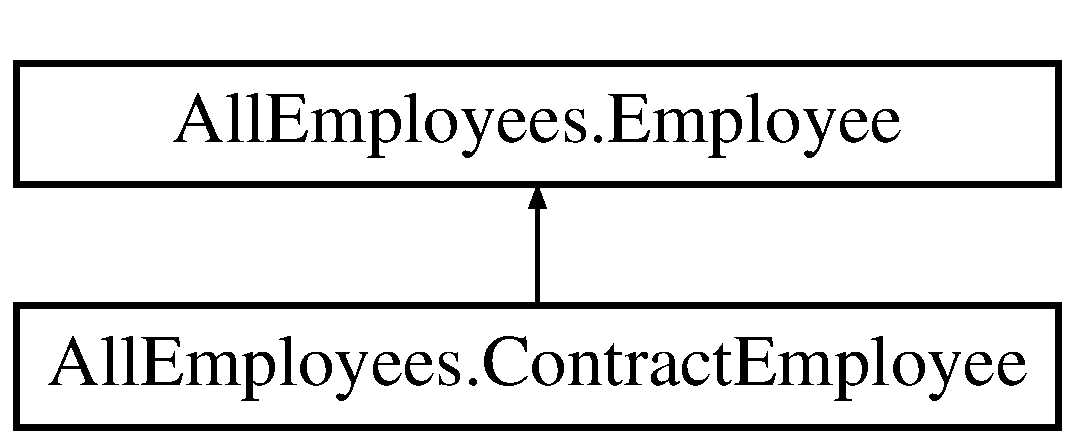
\includegraphics[height=2.000000cm]{class_all_employees_1_1_contract_employee}
\end{center}
\end{figure}
\subsection*{Public Member Functions}
\begin{DoxyCompactItemize}
\item 
\hyperlink{class_all_employees_1_1_contract_employee_afb78892e913ff2a34aed4d7b78d6c9f7}{Contract\+Employee} ()
\begin{DoxyCompactList}\small\item\em default constructor. Sets all values to default \end{DoxyCompactList}\item 
\hyperlink{class_all_employees_1_1_contract_employee_ac7aa7412d0f08a2176da6e9fc0a1ddba}{Contract\+Employee} (string first\+Name, string last\+Name)
\begin{DoxyCompactList}\small\item\em overloaded constructor. Sets name to inputed names, set all other values to default \end{DoxyCompactList}\item 
\hyperlink{class_all_employees_1_1_contract_employee_ad5a58ffe16b3b193e6024219a6b10174}{Contract\+Employee} (string first\+Name, string last\+Name, int social\+Insurance\+Number, Date\+Time date\+Of\+Birth, Date\+Time contract\+Start\+Date, Date\+Time contract\+Stop\+Date, float fixed\+Contract\+Amount)
\begin{DoxyCompactList}\small\item\em overloaded constructor. Sets all values to the values given. no default values \end{DoxyCompactList}\item 
bool \hyperlink{class_all_employees_1_1_contract_employee_a826e3f824d86fb6b4cd1c527350c5b3a}{Validate} ()
\begin{DoxyCompactList}\small\item\em Used to determine in the object contains a valid employee. \end{DoxyCompactList}\item 
string \hyperlink{class_all_employees_1_1_contract_employee_adc3a5e1e3280ac1ec77d1a0767b95c19}{Details} ()
\begin{DoxyCompactList}\small\item\em Used to create a formated string of all employee to be printed to the screen. \end{DoxyCompactList}\item 
override string \hyperlink{class_all_employees_1_1_contract_employee_ae0ba5deffac9dcf5317c91fd7d7f8816}{To\+String} ()
\begin{DoxyCompactList}\small\item\em Overriden method To\+String used to return a formated string of all data about employee. \end{DoxyCompactList}\item 
bool \hyperlink{class_all_employees_1_1_contract_employee_a012c48affde48858bda39a3cb9c802c4}{Set\+Contract\+Start\+Date} (Date\+Time date)
\begin{DoxyCompactList}\small\item\em Setter for contract\+Start\+Date from Date\+Time. \end{DoxyCompactList}\item 
bool \hyperlink{class_all_employees_1_1_contract_employee_aa10c777bc6b24385ceffaaff118e996e}{Set\+Contract\+Start\+Date} (string date)
\begin{DoxyCompactList}\small\item\em Setter for contract\+Start\+Date from String. \end{DoxyCompactList}\item 
bool \hyperlink{class_all_employees_1_1_contract_employee_af29121fe33b4f31b28eb545235a31331}{Set\+Contract\+Start\+Date} (int year, int month, int day)
\begin{DoxyCompactList}\small\item\em Setter for contract\+Start\+Date from ints. \end{DoxyCompactList}\item 
bool \hyperlink{class_all_employees_1_1_contract_employee_a60d9959aaf0368d3d951e00dc9b9276b}{Set\+Contract\+Stop\+Date} (Date\+Time date)
\begin{DoxyCompactList}\small\item\em Setter for contract\+Stop\+Date from Date\+Time. \end{DoxyCompactList}\item 
bool \hyperlink{class_all_employees_1_1_contract_employee_a5564f971606a6c44977001b3faef78d1}{Set\+Contract\+Stop\+Date} (string date)
\begin{DoxyCompactList}\small\item\em Setter for contract\+Stop\+Date from string. \end{DoxyCompactList}\item 
bool \hyperlink{class_all_employees_1_1_contract_employee_a3f7473cd491df8b2927333287b57a33d}{Set\+Contract\+Stop\+Date} (int year, int month, int day)
\begin{DoxyCompactList}\small\item\em Setter for contract\+Stop\+Date from ints. \end{DoxyCompactList}\item 
bool \hyperlink{class_all_employees_1_1_contract_employee_acf577438381bc6c56bc8f70ce0b25111}{Set\+Fixed\+Contract\+Amount} (float contract\+Amount)
\begin{DoxyCompactList}\small\item\em Setter for fixed\+Contract\+Amount. \end{DoxyCompactList}\item 
Date\+Time \hyperlink{class_all_employees_1_1_contract_employee_a270e070d2ccf2f707c9441f0ba1f2fad}{Get\+Contract\+Start\+Date} ()
\begin{DoxyCompactList}\small\item\em Getter for contract\+Start\+Date that returns Date\+Time. \end{DoxyCompactList}\item 
string \hyperlink{class_all_employees_1_1_contract_employee_a706f9a356995be719add2e1d522d1625}{Get\+Contract\+Start\+Date\+String} ()
\begin{DoxyCompactList}\small\item\em Getter for contract\+Start\+Date that returns formatted string. \end{DoxyCompactList}\item 
Date\+Time \hyperlink{class_all_employees_1_1_contract_employee_a98cacd6f03b693ba838b36c861c59b10}{Get\+Contract\+Stop\+Date} ()
\begin{DoxyCompactList}\small\item\em Getter for contract\+Stop\+Date that returns Date\+Time. \end{DoxyCompactList}\item 
string \hyperlink{class_all_employees_1_1_contract_employee_ada12137c290146af671d8e9b8db2b3fa}{Get\+Contract\+Stop\+Date\+String} ()
\begin{DoxyCompactList}\small\item\em Getter for contract\+Stop\+Date that returns formatted string. \end{DoxyCompactList}\item 
float \hyperlink{class_all_employees_1_1_contract_employee_add493d299c7d7ea7a8f8983aee2e5fa0}{Get\+Fixed\+Contract\+Amount} ()
\begin{DoxyCompactList}\small\item\em Getter for fixed\+Contract\+Amount. \end{DoxyCompactList}\end{DoxyCompactItemize}
\subsection*{Private Attributes}
\begin{DoxyCompactItemize}
\item 
\hypertarget{class_all_employees_1_1_contract_employee_aeef462cc8bd0639b674bba0632b6586b}{}Date\+Time {\bfseries contract\+Start\+Date}\label{class_all_employees_1_1_contract_employee_aeef462cc8bd0639b674bba0632b6586b}

\item 
\hypertarget{class_all_employees_1_1_contract_employee_ab549d2c8addad182fd66246c41ca73b7}{}Date\+Time {\bfseries contract\+Stop\+Date}\label{class_all_employees_1_1_contract_employee_ab549d2c8addad182fd66246c41ca73b7}

\item 
\hypertarget{class_all_employees_1_1_contract_employee_a81526f8517894ce466b70e3ffa61a8a8}{}float {\bfseries fixed\+Contract\+Amount}\label{class_all_employees_1_1_contract_employee_a81526f8517894ce466b70e3ffa61a8a8}

\end{DoxyCompactItemize}
\subsection*{Additional Inherited Members}


\subsection{Detailed Description}
{\bfseries Brief Description} The Contract \hyperlink{class_all_employees_1_1_employee}{Employee} class is used to store and manage data about a employee who is hired on a contract This class is a child to \hyperlink{class_all_employees_1_1_employee}{Employee} class. It adds the contract start and stop date and the amout the employee is payed for the contract The base classes Social Insurance Number is treated as a buisness number for this class. 

\begin{DoxyAuthor}{Author}
{\itshape Brandon} 
\end{DoxyAuthor}


\subsection{Constructor \& Destructor Documentation}
\hypertarget{class_all_employees_1_1_contract_employee_afb78892e913ff2a34aed4d7b78d6c9f7}{}\index{All\+Employees\+::\+Contract\+Employee@{All\+Employees\+::\+Contract\+Employee}!Contract\+Employee@{Contract\+Employee}}
\index{Contract\+Employee@{Contract\+Employee}!All\+Employees\+::\+Contract\+Employee@{All\+Employees\+::\+Contract\+Employee}}
\subsubsection[{Contract\+Employee}]{\setlength{\rightskip}{0pt plus 5cm}All\+Employees.\+Contract\+Employee.\+Contract\+Employee (
\begin{DoxyParamCaption}
{}
\end{DoxyParamCaption}
)}\label{class_all_employees_1_1_contract_employee_afb78892e913ff2a34aed4d7b78d6c9f7}


default constructor. Sets all values to default 

{\bfseries Details}


\begin{DoxyParams}{Parameters}
{\em n/a} & \\
\hline
\end{DoxyParams}
\begin{DoxyReturn}{Returns}
n/a 
\end{DoxyReturn}
\hypertarget{class_all_employees_1_1_contract_employee_ac7aa7412d0f08a2176da6e9fc0a1ddba}{}\index{All\+Employees\+::\+Contract\+Employee@{All\+Employees\+::\+Contract\+Employee}!Contract\+Employee@{Contract\+Employee}}
\index{Contract\+Employee@{Contract\+Employee}!All\+Employees\+::\+Contract\+Employee@{All\+Employees\+::\+Contract\+Employee}}
\subsubsection[{Contract\+Employee}]{\setlength{\rightskip}{0pt plus 5cm}All\+Employees.\+Contract\+Employee.\+Contract\+Employee (
\begin{DoxyParamCaption}
\item[{string}]{first\+Name, }
\item[{string}]{last\+Name}
\end{DoxyParamCaption}
)}\label{class_all_employees_1_1_contract_employee_ac7aa7412d0f08a2176da6e9fc0a1ddba}


overloaded constructor. Sets name to inputed names, set all other values to default 

{\bfseries Details}


\begin{DoxyParams}{Parameters}
{\em first\+Name} & -\/ {\bfseries string} -\/ First Name of employee to add to records \\
\hline
{\em last\+Name} & -\/ {\bfseries string} -\/ Last Name of employee to add to records\\
\hline
\end{DoxyParams}

\begin{DoxyExceptions}{Exceptions}
{\em $<$\+Failed\+Constructor\+Exception$>$} & -\/ If the constructor failed to create the object\\
\hline
\end{DoxyExceptions}
\begin{DoxyReturn}{Returns}
n/a 
\end{DoxyReturn}
\hypertarget{class_all_employees_1_1_contract_employee_ad5a58ffe16b3b193e6024219a6b10174}{}\index{All\+Employees\+::\+Contract\+Employee@{All\+Employees\+::\+Contract\+Employee}!Contract\+Employee@{Contract\+Employee}}
\index{Contract\+Employee@{Contract\+Employee}!All\+Employees\+::\+Contract\+Employee@{All\+Employees\+::\+Contract\+Employee}}
\subsubsection[{Contract\+Employee}]{\setlength{\rightskip}{0pt plus 5cm}All\+Employees.\+Contract\+Employee.\+Contract\+Employee (
\begin{DoxyParamCaption}
\item[{string}]{first\+Name, }
\item[{string}]{last\+Name, }
\item[{int}]{social\+Insurance\+Number, }
\item[{Date\+Time}]{date\+Of\+Birth, }
\item[{Date\+Time}]{contract\+Start\+Date, }
\item[{Date\+Time}]{contract\+Stop\+Date, }
\item[{float}]{fixed\+Contract\+Amount}
\end{DoxyParamCaption}
)}\label{class_all_employees_1_1_contract_employee_ad5a58ffe16b3b193e6024219a6b10174}


overloaded constructor. Sets all values to the values given. no default values 

{\bfseries Details}


\begin{DoxyParams}{Parameters}
{\em first\+Name} & -\/ {\bfseries string} -\/ First Name of employee to add to records \\
\hline
{\em last\+Name} & -\/ {\bfseries string} -\/ Last Name of employee to add to records \\
\hline
{\em social\+Insurance\+Number} & -\/ {\bfseries int} -\/ Social Insurance Number of employee to add to records \\
\hline
{\em date\+Of\+Birth} & -\/ {\bfseries Date\+Time} -\/ Date Of Birth of employee to add to records \\
\hline
{\em contract\+Start\+Date} & -\/ {\bfseries Date\+Time} -\/ Contract Start Date of employee contract to add to records \\
\hline
{\em contract\+Stop\+Date} & -\/ {\bfseries Date\+Time} -\/ Contract Stop Date of employee contract to add to records \\
\hline
{\em fixed\+Contract\+Amount} & -\/ {\bfseries float} -\/ Fixed Contract Amount of employee contract to add to records\\
\hline
\end{DoxyParams}

\begin{DoxyExceptions}{Exceptions}
{\em $<$\+Failed\+Constructor\+Exception$>$} & -\/ If the constructor failed to create the object\\
\hline
\end{DoxyExceptions}
\begin{DoxyReturn}{Returns}
n/a 
\end{DoxyReturn}


\subsection{Member Function Documentation}
\hypertarget{class_all_employees_1_1_contract_employee_adc3a5e1e3280ac1ec77d1a0767b95c19}{}\index{All\+Employees\+::\+Contract\+Employee@{All\+Employees\+::\+Contract\+Employee}!Details@{Details}}
\index{Details@{Details}!All\+Employees\+::\+Contract\+Employee@{All\+Employees\+::\+Contract\+Employee}}
\subsubsection[{Details}]{\setlength{\rightskip}{0pt plus 5cm}string All\+Employees.\+Contract\+Employee.\+Details (
\begin{DoxyParamCaption}
{}
\end{DoxyParamCaption}
)}\label{class_all_employees_1_1_contract_employee_adc3a5e1e3280ac1ec77d1a0767b95c19}


Used to create a formated string of all employee to be printed to the screen. 

{\bfseries Details}


\begin{DoxyParams}{Parameters}
{\em n/a} & \\
\hline
\end{DoxyParams}
\begin{DoxyReturn}{Returns}
user\+Info {\bfseries string} -\/ formatted string of employee data 
\end{DoxyReturn}
\hypertarget{class_all_employees_1_1_contract_employee_a270e070d2ccf2f707c9441f0ba1f2fad}{}\index{All\+Employees\+::\+Contract\+Employee@{All\+Employees\+::\+Contract\+Employee}!Get\+Contract\+Start\+Date@{Get\+Contract\+Start\+Date}}
\index{Get\+Contract\+Start\+Date@{Get\+Contract\+Start\+Date}!All\+Employees\+::\+Contract\+Employee@{All\+Employees\+::\+Contract\+Employee}}
\subsubsection[{Get\+Contract\+Start\+Date}]{\setlength{\rightskip}{0pt plus 5cm}Date\+Time All\+Employees.\+Contract\+Employee.\+Get\+Contract\+Start\+Date (
\begin{DoxyParamCaption}
{}
\end{DoxyParamCaption}
)}\label{class_all_employees_1_1_contract_employee_a270e070d2ccf2f707c9441f0ba1f2fad}


Getter for contract\+Start\+Date that returns Date\+Time. 

{\bfseries Details}


\begin{DoxyParams}{Parameters}
{\em n/a} & \\
\hline
\end{DoxyParams}
\begin{DoxyReturn}{Returns}
contract\+Start\+Date {\bfseries Date\+Time} 
\end{DoxyReturn}
\hypertarget{class_all_employees_1_1_contract_employee_a706f9a356995be719add2e1d522d1625}{}\index{All\+Employees\+::\+Contract\+Employee@{All\+Employees\+::\+Contract\+Employee}!Get\+Contract\+Start\+Date\+String@{Get\+Contract\+Start\+Date\+String}}
\index{Get\+Contract\+Start\+Date\+String@{Get\+Contract\+Start\+Date\+String}!All\+Employees\+::\+Contract\+Employee@{All\+Employees\+::\+Contract\+Employee}}
\subsubsection[{Get\+Contract\+Start\+Date\+String}]{\setlength{\rightskip}{0pt plus 5cm}string All\+Employees.\+Contract\+Employee.\+Get\+Contract\+Start\+Date\+String (
\begin{DoxyParamCaption}
{}
\end{DoxyParamCaption}
)}\label{class_all_employees_1_1_contract_employee_a706f9a356995be719add2e1d522d1625}


Getter for contract\+Start\+Date that returns formatted string. 

{\bfseries Details}


\begin{DoxyParams}{Parameters}
{\em n/a} & \\
\hline
\end{DoxyParams}
\begin{DoxyReturn}{Returns}
contract\+Start\+Date {\bfseries string} 
\end{DoxyReturn}
\hypertarget{class_all_employees_1_1_contract_employee_a98cacd6f03b693ba838b36c861c59b10}{}\index{All\+Employees\+::\+Contract\+Employee@{All\+Employees\+::\+Contract\+Employee}!Get\+Contract\+Stop\+Date@{Get\+Contract\+Stop\+Date}}
\index{Get\+Contract\+Stop\+Date@{Get\+Contract\+Stop\+Date}!All\+Employees\+::\+Contract\+Employee@{All\+Employees\+::\+Contract\+Employee}}
\subsubsection[{Get\+Contract\+Stop\+Date}]{\setlength{\rightskip}{0pt plus 5cm}Date\+Time All\+Employees.\+Contract\+Employee.\+Get\+Contract\+Stop\+Date (
\begin{DoxyParamCaption}
{}
\end{DoxyParamCaption}
)}\label{class_all_employees_1_1_contract_employee_a98cacd6f03b693ba838b36c861c59b10}


Getter for contract\+Stop\+Date that returns Date\+Time. 

{\bfseries Details}


\begin{DoxyParams}{Parameters}
{\em n/a} & \\
\hline
\end{DoxyParams}
\begin{DoxyReturn}{Returns}
contract\+Stop\+Date {\bfseries Date\+Time} 
\end{DoxyReturn}
\hypertarget{class_all_employees_1_1_contract_employee_ada12137c290146af671d8e9b8db2b3fa}{}\index{All\+Employees\+::\+Contract\+Employee@{All\+Employees\+::\+Contract\+Employee}!Get\+Contract\+Stop\+Date\+String@{Get\+Contract\+Stop\+Date\+String}}
\index{Get\+Contract\+Stop\+Date\+String@{Get\+Contract\+Stop\+Date\+String}!All\+Employees\+::\+Contract\+Employee@{All\+Employees\+::\+Contract\+Employee}}
\subsubsection[{Get\+Contract\+Stop\+Date\+String}]{\setlength{\rightskip}{0pt plus 5cm}string All\+Employees.\+Contract\+Employee.\+Get\+Contract\+Stop\+Date\+String (
\begin{DoxyParamCaption}
{}
\end{DoxyParamCaption}
)}\label{class_all_employees_1_1_contract_employee_ada12137c290146af671d8e9b8db2b3fa}


Getter for contract\+Stop\+Date that returns formatted string. 

{\bfseries Details}


\begin{DoxyParams}{Parameters}
{\em n/a} & \\
\hline
\end{DoxyParams}
\begin{DoxyReturn}{Returns}
contract\+Stop\+Date {\bfseries string} 
\end{DoxyReturn}
\hypertarget{class_all_employees_1_1_contract_employee_add493d299c7d7ea7a8f8983aee2e5fa0}{}\index{All\+Employees\+::\+Contract\+Employee@{All\+Employees\+::\+Contract\+Employee}!Get\+Fixed\+Contract\+Amount@{Get\+Fixed\+Contract\+Amount}}
\index{Get\+Fixed\+Contract\+Amount@{Get\+Fixed\+Contract\+Amount}!All\+Employees\+::\+Contract\+Employee@{All\+Employees\+::\+Contract\+Employee}}
\subsubsection[{Get\+Fixed\+Contract\+Amount}]{\setlength{\rightskip}{0pt plus 5cm}float All\+Employees.\+Contract\+Employee.\+Get\+Fixed\+Contract\+Amount (
\begin{DoxyParamCaption}
{}
\end{DoxyParamCaption}
)}\label{class_all_employees_1_1_contract_employee_add493d299c7d7ea7a8f8983aee2e5fa0}


Getter for fixed\+Contract\+Amount. 

{\bfseries Details}


\begin{DoxyParams}{Parameters}
{\em n/a} & \\
\hline
\end{DoxyParams}
\begin{DoxyReturn}{Returns}
fixed\+Contract\+Amount {\bfseries float} 
\end{DoxyReturn}
\hypertarget{class_all_employees_1_1_contract_employee_a012c48affde48858bda39a3cb9c802c4}{}\index{All\+Employees\+::\+Contract\+Employee@{All\+Employees\+::\+Contract\+Employee}!Set\+Contract\+Start\+Date@{Set\+Contract\+Start\+Date}}
\index{Set\+Contract\+Start\+Date@{Set\+Contract\+Start\+Date}!All\+Employees\+::\+Contract\+Employee@{All\+Employees\+::\+Contract\+Employee}}
\subsubsection[{Set\+Contract\+Start\+Date}]{\setlength{\rightskip}{0pt plus 5cm}bool All\+Employees.\+Contract\+Employee.\+Set\+Contract\+Start\+Date (
\begin{DoxyParamCaption}
\item[{Date\+Time}]{date}
\end{DoxyParamCaption}
)}\label{class_all_employees_1_1_contract_employee_a012c48affde48858bda39a3cb9c802c4}


Setter for contract\+Start\+Date from Date\+Time. 

{\bfseries Details}


\begin{DoxyParams}{Parameters}
{\em date} & {\bfseries Date\+Time} -\/ The start date of the employees contract\\
\hline
\end{DoxyParams}
\begin{DoxyReturn}{Returns}
data\+Saved {\bfseries bool} -\/ true if input was valid and data was changed. False it data was not changed 
\end{DoxyReturn}
\hypertarget{class_all_employees_1_1_contract_employee_aa10c777bc6b24385ceffaaff118e996e}{}\index{All\+Employees\+::\+Contract\+Employee@{All\+Employees\+::\+Contract\+Employee}!Set\+Contract\+Start\+Date@{Set\+Contract\+Start\+Date}}
\index{Set\+Contract\+Start\+Date@{Set\+Contract\+Start\+Date}!All\+Employees\+::\+Contract\+Employee@{All\+Employees\+::\+Contract\+Employee}}
\subsubsection[{Set\+Contract\+Start\+Date}]{\setlength{\rightskip}{0pt plus 5cm}bool All\+Employees.\+Contract\+Employee.\+Set\+Contract\+Start\+Date (
\begin{DoxyParamCaption}
\item[{string}]{date}
\end{DoxyParamCaption}
)}\label{class_all_employees_1_1_contract_employee_aa10c777bc6b24385ceffaaff118e996e}


Setter for contract\+Start\+Date from String. 

{\bfseries Details}


\begin{DoxyParams}{Parameters}
{\em date} & {\bfseries string} -\/ The start date of the employees contract\\
\hline
\end{DoxyParams}
\begin{DoxyReturn}{Returns}
data\+Saved {\bfseries bool} -\/ true if input was valid and data was changed. False it data was not changed 
\end{DoxyReturn}
\hypertarget{class_all_employees_1_1_contract_employee_af29121fe33b4f31b28eb545235a31331}{}\index{All\+Employees\+::\+Contract\+Employee@{All\+Employees\+::\+Contract\+Employee}!Set\+Contract\+Start\+Date@{Set\+Contract\+Start\+Date}}
\index{Set\+Contract\+Start\+Date@{Set\+Contract\+Start\+Date}!All\+Employees\+::\+Contract\+Employee@{All\+Employees\+::\+Contract\+Employee}}
\subsubsection[{Set\+Contract\+Start\+Date}]{\setlength{\rightskip}{0pt plus 5cm}bool All\+Employees.\+Contract\+Employee.\+Set\+Contract\+Start\+Date (
\begin{DoxyParamCaption}
\item[{int}]{year, }
\item[{int}]{month, }
\item[{int}]{day}
\end{DoxyParamCaption}
)}\label{class_all_employees_1_1_contract_employee_af29121fe33b4f31b28eb545235a31331}


Setter for contract\+Start\+Date from ints. 

{\bfseries Details}


\begin{DoxyParams}{Parameters}
{\em year} & {\bfseries int} -\/ The start year of the employees contract \\
\hline
{\em month} & {\bfseries int} -\/ The start month of the employees contract \\
\hline
{\em day} & {\bfseries int} -\/ The start day of the employees contract\\
\hline
\end{DoxyParams}
\begin{DoxyReturn}{Returns}
data\+Saved {\bfseries bool} -\/ true if input was valid and data was changed. False it data was not changed 
\end{DoxyReturn}
\hypertarget{class_all_employees_1_1_contract_employee_a60d9959aaf0368d3d951e00dc9b9276b}{}\index{All\+Employees\+::\+Contract\+Employee@{All\+Employees\+::\+Contract\+Employee}!Set\+Contract\+Stop\+Date@{Set\+Contract\+Stop\+Date}}
\index{Set\+Contract\+Stop\+Date@{Set\+Contract\+Stop\+Date}!All\+Employees\+::\+Contract\+Employee@{All\+Employees\+::\+Contract\+Employee}}
\subsubsection[{Set\+Contract\+Stop\+Date}]{\setlength{\rightskip}{0pt plus 5cm}bool All\+Employees.\+Contract\+Employee.\+Set\+Contract\+Stop\+Date (
\begin{DoxyParamCaption}
\item[{Date\+Time}]{date}
\end{DoxyParamCaption}
)}\label{class_all_employees_1_1_contract_employee_a60d9959aaf0368d3d951e00dc9b9276b}


Setter for contract\+Stop\+Date from Date\+Time. 

{\bfseries Details}


\begin{DoxyParams}{Parameters}
{\em date} & {\bfseries Date\+Time} -\/ The stop date of the employees contract\\
\hline
\end{DoxyParams}
\begin{DoxyReturn}{Returns}
data\+Saved {\bfseries bool} -\/ true if input was valid and data was changed. False it data was not changed 
\end{DoxyReturn}
\hypertarget{class_all_employees_1_1_contract_employee_a5564f971606a6c44977001b3faef78d1}{}\index{All\+Employees\+::\+Contract\+Employee@{All\+Employees\+::\+Contract\+Employee}!Set\+Contract\+Stop\+Date@{Set\+Contract\+Stop\+Date}}
\index{Set\+Contract\+Stop\+Date@{Set\+Contract\+Stop\+Date}!All\+Employees\+::\+Contract\+Employee@{All\+Employees\+::\+Contract\+Employee}}
\subsubsection[{Set\+Contract\+Stop\+Date}]{\setlength{\rightskip}{0pt plus 5cm}bool All\+Employees.\+Contract\+Employee.\+Set\+Contract\+Stop\+Date (
\begin{DoxyParamCaption}
\item[{string}]{date}
\end{DoxyParamCaption}
)}\label{class_all_employees_1_1_contract_employee_a5564f971606a6c44977001b3faef78d1}


Setter for contract\+Stop\+Date from string. 

{\bfseries Details}


\begin{DoxyParams}{Parameters}
{\em date} & {\bfseries string} -\/ The stop date of the employees contract\\
\hline
\end{DoxyParams}
\begin{DoxyReturn}{Returns}
data\+Saved {\bfseries bool} -\/ true if input was valid and data was changed. False it data was not changed 
\end{DoxyReturn}
\hypertarget{class_all_employees_1_1_contract_employee_a3f7473cd491df8b2927333287b57a33d}{}\index{All\+Employees\+::\+Contract\+Employee@{All\+Employees\+::\+Contract\+Employee}!Set\+Contract\+Stop\+Date@{Set\+Contract\+Stop\+Date}}
\index{Set\+Contract\+Stop\+Date@{Set\+Contract\+Stop\+Date}!All\+Employees\+::\+Contract\+Employee@{All\+Employees\+::\+Contract\+Employee}}
\subsubsection[{Set\+Contract\+Stop\+Date}]{\setlength{\rightskip}{0pt plus 5cm}bool All\+Employees.\+Contract\+Employee.\+Set\+Contract\+Stop\+Date (
\begin{DoxyParamCaption}
\item[{int}]{year, }
\item[{int}]{month, }
\item[{int}]{day}
\end{DoxyParamCaption}
)}\label{class_all_employees_1_1_contract_employee_a3f7473cd491df8b2927333287b57a33d}


Setter for contract\+Stop\+Date from ints. 

{\bfseries Details}


\begin{DoxyParams}{Parameters}
{\em year} & {\bfseries int} -\/ The stop year of the employees contract \\
\hline
{\em month} & {\bfseries int} -\/ The stop month of the employees contract \\
\hline
{\em day} & {\bfseries int} -\/ The stop day of the employees contract\\
\hline
\end{DoxyParams}
\begin{DoxyReturn}{Returns}
data\+Saved {\bfseries bool} -\/ true if input was valid and data was changed. False it data was not changed 
\end{DoxyReturn}
\hypertarget{class_all_employees_1_1_contract_employee_acf577438381bc6c56bc8f70ce0b25111}{}\index{All\+Employees\+::\+Contract\+Employee@{All\+Employees\+::\+Contract\+Employee}!Set\+Fixed\+Contract\+Amount@{Set\+Fixed\+Contract\+Amount}}
\index{Set\+Fixed\+Contract\+Amount@{Set\+Fixed\+Contract\+Amount}!All\+Employees\+::\+Contract\+Employee@{All\+Employees\+::\+Contract\+Employee}}
\subsubsection[{Set\+Fixed\+Contract\+Amount}]{\setlength{\rightskip}{0pt plus 5cm}bool All\+Employees.\+Contract\+Employee.\+Set\+Fixed\+Contract\+Amount (
\begin{DoxyParamCaption}
\item[{float}]{contract\+Amount}
\end{DoxyParamCaption}
)}\label{class_all_employees_1_1_contract_employee_acf577438381bc6c56bc8f70ce0b25111}


Setter for fixed\+Contract\+Amount. 

{\bfseries Details}


\begin{DoxyParams}{Parameters}
{\em contract\+Amount} & {\bfseries float} -\/ The amount the contract is payed\\
\hline
\end{DoxyParams}
\begin{DoxyReturn}{Returns}
data\+Saves {\bfseries bool} -\/ true if input was valid and data was changed. False it data was not changed 
\end{DoxyReturn}
\hypertarget{class_all_employees_1_1_contract_employee_ae0ba5deffac9dcf5317c91fd7d7f8816}{}\index{All\+Employees\+::\+Contract\+Employee@{All\+Employees\+::\+Contract\+Employee}!To\+String@{To\+String}}
\index{To\+String@{To\+String}!All\+Employees\+::\+Contract\+Employee@{All\+Employees\+::\+Contract\+Employee}}
\subsubsection[{To\+String}]{\setlength{\rightskip}{0pt plus 5cm}override string All\+Employees.\+Contract\+Employee.\+To\+String (
\begin{DoxyParamCaption}
{}
\end{DoxyParamCaption}
)}\label{class_all_employees_1_1_contract_employee_ae0ba5deffac9dcf5317c91fd7d7f8816}


Overriden method To\+String used to return a formated string of all data about employee. 

{\bfseries Details}


\begin{DoxyParams}{Parameters}
{\em n/a} & \\
\hline
\end{DoxyParams}
\begin{DoxyReturn}{Returns}
employee\+String {\bfseries string} -\/ the formated string containing all employee data 
\end{DoxyReturn}
\hypertarget{class_all_employees_1_1_contract_employee_a826e3f824d86fb6b4cd1c527350c5b3a}{}\index{All\+Employees\+::\+Contract\+Employee@{All\+Employees\+::\+Contract\+Employee}!Validate@{Validate}}
\index{Validate@{Validate}!All\+Employees\+::\+Contract\+Employee@{All\+Employees\+::\+Contract\+Employee}}
\subsubsection[{Validate}]{\setlength{\rightskip}{0pt plus 5cm}bool All\+Employees.\+Contract\+Employee.\+Validate (
\begin{DoxyParamCaption}
{}
\end{DoxyParamCaption}
)}\label{class_all_employees_1_1_contract_employee_a826e3f824d86fb6b4cd1c527350c5b3a}


Used to determine in the object contains a valid employee. 

{\bfseries Details}


\begin{DoxyParams}{Parameters}
{\em n/a} & \\
\hline
\end{DoxyParams}
\begin{DoxyReturn}{Returns}
data\+Valid -\/ {\bfseries bool} -\/ True if the object contains all data for a valid employee 
\end{DoxyReturn}


The documentation for this class was generated from the following file\+:\begin{DoxyCompactItemize}
\item 
C\+:/\+S\+E\+T\+Repo/trunk/\+E\+M\+S/trunk/\+All\+Employees/\+All\+Employees/Contract\+Employee.\+cs\end{DoxyCompactItemize}

\hypertarget{class_my_all_employee_1_1_tests_1_1_contract_employee_tests}{}\section{My\+All\+Employee.\+Tests.\+Contract\+Employee\+Tests Class Reference}
\label{class_my_all_employee_1_1_tests_1_1_contract_employee_tests}\index{My\+All\+Employee.\+Tests.\+Contract\+Employee\+Tests@{My\+All\+Employee.\+Tests.\+Contract\+Employee\+Tests}}


{\bfseries  Brief Description} This class is used to test the Contract\+Employee methods in the All\+Employee class. The methods tested include the constructors, Details, Set\+Date\+Of\+Birth (all 3 overloaded methods), Set\+Contract\+Date (all 3 overloaded methods), Set\+Contract\+Stop\+Date(all 3 overloaded methods), Set\+Fixed\+Cntract\+Amount and To\+String.  


\subsection*{Public Member Functions}
\begin{DoxyCompactItemize}
\item 
void \hyperlink{class_my_all_employee_1_1_tests_1_1_contract_employee_tests_a8924368697df663c9bc44cb8b07c07f3}{Constructor\+With\+Names\+Test\+Valid1} ()
\begin{DoxyCompactList}\small\item\em This unit test will check if either name contains anything other than a letter, apostrophe, dash. It will throw an exception if wrong. \end{DoxyCompactList}\item 
void \hyperlink{class_my_all_employee_1_1_tests_1_1_contract_employee_tests_abdd736e2305faf27435f9366b9fa6dd5}{Constructor\+With\+Names\+Test\+Valid2} ()
\begin{DoxyCompactList}\small\item\em This unit test will check if either name contains anything other than a letter, apostrophe, dash. It will throw an exception if wrong. \end{DoxyCompactList}\item 
void \hyperlink{class_my_all_employee_1_1_tests_1_1_contract_employee_tests_ac6d1169e3a43330cffcabfb4d4d68f40}{Constructor\+With\+Names\+Test\+Valid3} ()
\begin{DoxyCompactList}\small\item\em This unit test will check if either name contains anything other than a letter, apostrophe, dash. It will throw an exception if wrong. \end{DoxyCompactList}\item 
void \hyperlink{class_my_all_employee_1_1_tests_1_1_contract_employee_tests_a243e3bc826eb636390c094b8d321078e}{Constructor\+With\+Names\+Test\+Invalid\+Slash} ()
\begin{DoxyCompactList}\small\item\em This unit test will check if the constructor will fail and if the string is invalid because it contains a slash. \end{DoxyCompactList}\item 
void \hyperlink{class_my_all_employee_1_1_tests_1_1_contract_employee_tests_a158688b964e7a096f4260a4b2fbcfd78}{Constructor\+With\+Names\+Test\+Invalid\+Space} ()
\begin{DoxyCompactList}\small\item\em This unit test will check if the constructor will fail and if the string is invalid because it contains a space. \end{DoxyCompactList}\item 
void \hyperlink{class_my_all_employee_1_1_tests_1_1_contract_employee_tests_adc02331d297288a96a4783174aa1adac}{Constructor\+With\+Names\+Test\+Invalid\+Number} ()
\begin{DoxyCompactList}\small\item\em This unit test will check if the constructor will fail and if the string is invalid because it contains a number. \end{DoxyCompactList}\item 
void \hyperlink{class_my_all_employee_1_1_tests_1_1_contract_employee_tests_aee5f3ae3e5e96ffe361e64ae8bb65f95}{Constructor\+With\+All\+Param\+Test\+Valid1} ()
\begin{DoxyCompactList}\small\item\em This unit test will check the constructor that takes in all possible parameters, and give them all valid data. \end{DoxyCompactList}\item 
void \hyperlink{class_my_all_employee_1_1_tests_1_1_contract_employee_tests_a41ab4eb534ed2853f3f732d5b6716937}{Constructor\+With\+All\+Param\+Test\+Valid2} ()
\begin{DoxyCompactList}\small\item\em This unit test will check the constructor that takes in all possible parameters, and give them all valid data. \end{DoxyCompactList}\item 
void \hyperlink{class_my_all_employee_1_1_tests_1_1_contract_employee_tests_a66f164a6382d2e57057d258bb2d18542}{Constructor\+With\+All\+Param\+Test\+Valid3} ()
\begin{DoxyCompactList}\small\item\em This unit test will check the constructor that takes in all possible parameters, and give them all valid data. \end{DoxyCompactList}\item 
void \hyperlink{class_my_all_employee_1_1_tests_1_1_contract_employee_tests_ae174629fed8b90f64fe7642e88252ec6}{Constructor\+With\+All\+Param\+Test\+Invalid\+B\+N} ()
\begin{DoxyCompactList}\small\item\em This unit test will check the constructor that takes in all possible parameters, and give them all invalid data. \end{DoxyCompactList}\item 
void \hyperlink{class_my_all_employee_1_1_tests_1_1_contract_employee_tests_ab7815f00ad5071df4eb6ffc855d51e17}{Constructor\+With\+All\+Param\+Test\+Invalid\+D\+O\+H\+Before\+D\+O\+B} ()
\begin{DoxyCompactList}\small\item\em This unit test will check the constructor that takes in all possible parameters, and give them all invalid data. \end{DoxyCompactList}\item 
void \hyperlink{class_my_all_employee_1_1_tests_1_1_contract_employee_tests_a036e75236b91f73f5c90513b6770c6b1}{Constructor\+With\+All\+Param\+Test\+Invalid\+D\+O\+T\+Bofore\+D\+O\+H} ()
\begin{DoxyCompactList}\small\item\em This unit test will check the constructor that takes in all possible parameters, and give them all invalid data. \end{DoxyCompactList}\item 
void \hyperlink{class_my_all_employee_1_1_tests_1_1_contract_employee_tests_a5a23d0f0d7baec8ebcfda76674b5fa65}{Constructor\+With\+All\+Param\+Test\+Invalid\+D\+O\+Tno\+D\+O\+H} ()
\begin{DoxyCompactList}\small\item\em This unit test will check the constructor that takes in all possible parameters, and give them all invalid data. \end{DoxyCompactList}\item 
void \hyperlink{class_my_all_employee_1_1_tests_1_1_contract_employee_tests_a97b02dfac3cfb319d67d5794fbb532ac}{Details\+Test\+Valid} ()
\begin{DoxyCompactList}\small\item\em This unit test will create an employee and runs it\textquotesingle{}s details, and will ensure that the string is what it should be(it is hardcoded) \end{DoxyCompactList}\item 
void \hyperlink{class_my_all_employee_1_1_tests_1_1_contract_employee_tests_a08805c288350931d63fdd171e097efb5}{Details\+Test\+Invalid\+No\+Date} ()
\begin{DoxyCompactList}\small\item\em This unit test will create an employee and runs it\textquotesingle{}s details, and will ensure that the string is not what it should be(it is hardcoded) \end{DoxyCompactList}\item 
void \hyperlink{class_my_all_employee_1_1_tests_1_1_contract_employee_tests_af20290a987245aae2cccc0ed7605f594}{To\+String\+Test\+Valid} ()
\begin{DoxyCompactList}\small\item\em This unit test will create an employee and runs it\textquotesingle{}s details, and will ensure that the string is what it should be(it is hardcoded) \end{DoxyCompactList}\item 
void \hyperlink{class_my_all_employee_1_1_tests_1_1_contract_employee_tests_a24545e0849679f5bef330efd01ed406e}{Set\+Contract\+Start\+Date\+Date\+Test\+Valid\+Date} ()
\begin{DoxyCompactList}\small\item\em This unit test will set the contract start date to a valid date. \end{DoxyCompactList}\item 
void \hyperlink{class_my_all_employee_1_1_tests_1_1_contract_employee_tests_ae10e97e6a955b9da89ffb268e01aa6c6}{Set\+Contract\+Start\+Date\+Date\+Test\+Invalid\+D\+O\+Hafter\+D\+O\+T} ()
\begin{DoxyCompactList}\small\item\em This unit test will set the contract start date to an invalid date. \end{DoxyCompactList}\item 
void \hyperlink{class_my_all_employee_1_1_tests_1_1_contract_employee_tests_a989034924eddd56877cf0838593b9602}{Set\+Contract\+Start\+Date\+String\+Test\+Invalid\+D\+O\+Hbefore\+D\+O\+B} ()
\begin{DoxyCompactList}\small\item\em This unit test will set the contract start date to an invalid date. \end{DoxyCompactList}\item 
void \hyperlink{class_my_all_employee_1_1_tests_1_1_contract_employee_tests_ac41ba86681724f03e8f1f85c3d359fea}{Set\+Contract\+Start\+Date\+String\+Test\+Valid\+String} ()
\begin{DoxyCompactList}\small\item\em This unit test will set the contract start string to a valid string. \end{DoxyCompactList}\item 
void \hyperlink{class_my_all_employee_1_1_tests_1_1_contract_employee_tests_a995964039ce3dc1dd4cbba72becf5f6c}{Set\+Contract\+Start\+Date\+String\+Test\+Invalid\+Format} ()
\begin{DoxyCompactList}\small\item\em This unit test will set the contract start string to an invalid string. \end{DoxyCompactList}\item 
void \hyperlink{class_my_all_employee_1_1_tests_1_1_contract_employee_tests_a27bedf46bccc7c5e28e72e81131b6e6a}{Set\+Contract\+Start\+Date\+String\+Test\+Invalid\+Date} ()
\begin{DoxyCompactList}\small\item\em This unit test will set the contract start string to an invalid string. \end{DoxyCompactList}\item 
void \hyperlink{class_my_all_employee_1_1_tests_1_1_contract_employee_tests_a891ba9b21cf8902876b83c54cc0c4851}{Set\+Contract\+Start\+Date\+String\+Test\+Invalid\+D\+O\+Hafter\+D\+O\+T} ()
\begin{DoxyCompactList}\small\item\em This unit test will set the contract start string to an invalid string. \end{DoxyCompactList}\item 
void \hyperlink{class_my_all_employee_1_1_tests_1_1_contract_employee_tests_ab2018211293ad52d299e8d253ade9536}{Set\+Contract\+Start\+Date\+Date\+Test\+Invalid\+D\+O\+Hbefore\+D\+O\+B} ()
\begin{DoxyCompactList}\small\item\em This unit test will set the contract start date to an invalid date. \end{DoxyCompactList}\item 
void \hyperlink{class_my_all_employee_1_1_tests_1_1_contract_employee_tests_a37a5d2abc21e0cc2eceacc10b82901ab}{Set\+Contract\+Start\+Date\+Ints\+Test\+Invalid\+Letter} ()
\begin{DoxyCompactList}\small\item\em This unit test will set the contract start date to an invalid date. \end{DoxyCompactList}\item 
void \hyperlink{class_my_all_employee_1_1_tests_1_1_contract_employee_tests_a3d5b0976b5a552242beaa1c36c24e000}{Set\+Contract\+Start\+Date\+Ints\+Test\+Valid} ()
\begin{DoxyCompactList}\small\item\em This unit test will set the contract start date to a valid date. \end{DoxyCompactList}\item 
void \hyperlink{class_my_all_employee_1_1_tests_1_1_contract_employee_tests_a1369f1d0638c30e10eaf7c47625c4120}{Set\+Contract\+Start\+Date\+Ints\+Test\+Invalid\+Date} ()
\begin{DoxyCompactList}\small\item\em This unit test will set the contract start date to an invalid date. \end{DoxyCompactList}\item 
void \hyperlink{class_my_all_employee_1_1_tests_1_1_contract_employee_tests_a9c422336c67090c4590edbd737ff4ab7}{Set\+Contract\+Start\+Date\+Ints\+Test\+Invalid\+D\+O\+Hafter\+D\+O\+T} ()
\begin{DoxyCompactList}\small\item\em This unit test will set the contract start date to an invalid date. \end{DoxyCompactList}\item 
void \hyperlink{class_my_all_employee_1_1_tests_1_1_contract_employee_tests_acecbb0788b2c0d2976aac21e06be62ee}{Set\+Contract\+Start\+Date\+Ints\+Test\+Invalid\+D\+O\+Hbefore\+D\+O\+B} ()
\begin{DoxyCompactList}\small\item\em This unit test will set the contract start date to an invalid date. \end{DoxyCompactList}\item 
void \hyperlink{class_my_all_employee_1_1_tests_1_1_contract_employee_tests_a29d11eaee911de4b54569f10f7c1702d}{Set\+Contract\+Stop\+Date\+Date\+Test\+Valid\+Date} ()
\begin{DoxyCompactList}\small\item\em This unit test will set the contract stop date to a valid date. \end{DoxyCompactList}\item 
void \hyperlink{class_my_all_employee_1_1_tests_1_1_contract_employee_tests_a353fe82d85914fe0d217d4668843df81}{Set\+Contract\+Stop\+Date\+Date\+Test\+Invalid\+D\+O\+Tbefore\+D\+O\+H} ()
\begin{DoxyCompactList}\small\item\em This unit test will set the contract stop date to an invalid date. \end{DoxyCompactList}\item 
void \hyperlink{class_my_all_employee_1_1_tests_1_1_contract_employee_tests_a0ed7d04ddfb7e0aaf1e6b4bf371c6b65}{Set\+Contract\+Stop\+Date\+String\+Test\+Valid\+String} ()
\begin{DoxyCompactList}\small\item\em This unit test will set the contract stop string to a valid string. \end{DoxyCompactList}\item 
void \hyperlink{class_my_all_employee_1_1_tests_1_1_contract_employee_tests_a261ee3cc3d3da92b06acdffbe32eb408}{Set\+Contract\+Stop\+Date\+String\+Test\+Invalid\+Format} ()
\begin{DoxyCompactList}\small\item\em This unit test will set the contract string date to an invalid string. \end{DoxyCompactList}\item 
void \hyperlink{class_my_all_employee_1_1_tests_1_1_contract_employee_tests_a9b30804b1769d8276ba81b1bf10f4f4b}{Set\+Contract\+Stop\+Date\+String\+Test\+Invalid\+Date} ()
\begin{DoxyCompactList}\small\item\em This unit test will set the contract stop string to an invalid string. \end{DoxyCompactList}\item 
void \hyperlink{class_my_all_employee_1_1_tests_1_1_contract_employee_tests_ab173ae0ba70332b83f2a10850c843d7a}{Set\+Contract\+Stop\+Date\+String\+Test\+Invalid\+D\+O\+Tbefore\+D\+O\+H} ()
\begin{DoxyCompactList}\small\item\em This unit test will set the contract stop string to an invalid string. \end{DoxyCompactList}\item 
void \hyperlink{class_my_all_employee_1_1_tests_1_1_contract_employee_tests_a1a2d4cb08d5d86536f12baef54cb2b3f}{Set\+Contract\+Stop\+Date\+Ints\+Test\+Invalid\+Letter} ()
\begin{DoxyCompactList}\small\item\em This unit test will set the contract stop date to an invalid date. \end{DoxyCompactList}\item 
void \hyperlink{class_my_all_employee_1_1_tests_1_1_contract_employee_tests_a9447df2cc82ad42e0fc164ae88e636a8}{Set\+Contract\+Stop\+Date\+Ints\+Test\+Valid} ()
\begin{DoxyCompactList}\small\item\em This unit test will set the contract stop date to a valid date. \end{DoxyCompactList}\item 
void \hyperlink{class_my_all_employee_1_1_tests_1_1_contract_employee_tests_aaa29e10f49c00d0f89db08a20d1fed48}{Set\+Contract\+Stop\+Date\+Ints\+Test\+Invalid\+Date} ()
\begin{DoxyCompactList}\small\item\em This unit test will set the contract stop date to an invalid date. \end{DoxyCompactList}\item 
void \hyperlink{class_my_all_employee_1_1_tests_1_1_contract_employee_tests_a4666e65ccf384f5d65f237cbd7205cc3}{Set\+Contract\+Stop\+Date\+Ints\+Test\+Invalid\+D\+O\+Tbefore\+D\+O\+H} ()
\begin{DoxyCompactList}\small\item\em This unit test will set the contract stop date to an invalid date. \end{DoxyCompactList}\item 
void \hyperlink{class_my_all_employee_1_1_tests_1_1_contract_employee_tests_a21fdcffc82d7dd616880c6de426ea608}{Set\+Fixed\+Contract\+Amount\+Valid} ()
\begin{DoxyCompactList}\small\item\em This unit test will set the fixed contract amount to a valid amount. \end{DoxyCompactList}\item 
void \hyperlink{class_my_all_employee_1_1_tests_1_1_contract_employee_tests_adbd5c9282fccead325fa1f04de809ffd}{Set\+Fixed\+Contract\+Amount\+Invalid\+Negitive} ()
\begin{DoxyCompactList}\small\item\em This unit test will set the fixed contract amount to an invalid amount. \end{DoxyCompactList}\end{DoxyCompactItemize}


\subsection{Detailed Description}
{\bfseries  Brief Description} This class is used to test the Contract\+Employee methods in the All\+Employee class. The methods tested include the constructors, Details, Set\+Date\+Of\+Birth (all 3 overloaded methods), Set\+Contract\+Date (all 3 overloaded methods), Set\+Contract\+Stop\+Date(all 3 overloaded methods), Set\+Fixed\+Cntract\+Amount and To\+String. 

\subsection{Member Function Documentation}
\hypertarget{class_my_all_employee_1_1_tests_1_1_contract_employee_tests_ae174629fed8b90f64fe7642e88252ec6}{}\index{My\+All\+Employee\+::\+Tests\+::\+Contract\+Employee\+Tests@{My\+All\+Employee\+::\+Tests\+::\+Contract\+Employee\+Tests}!Constructor\+With\+All\+Param\+Test\+Invalid\+B\+N@{Constructor\+With\+All\+Param\+Test\+Invalid\+B\+N}}
\index{Constructor\+With\+All\+Param\+Test\+Invalid\+B\+N@{Constructor\+With\+All\+Param\+Test\+Invalid\+B\+N}!My\+All\+Employee\+::\+Tests\+::\+Contract\+Employee\+Tests@{My\+All\+Employee\+::\+Tests\+::\+Contract\+Employee\+Tests}}
\subsubsection[{Constructor\+With\+All\+Param\+Test\+Invalid\+B\+N}]{\setlength{\rightskip}{0pt plus 5cm}void My\+All\+Employee.\+Tests.\+Contract\+Employee\+Tests.\+Constructor\+With\+All\+Param\+Test\+Invalid\+B\+N (
\begin{DoxyParamCaption}
{}
\end{DoxyParamCaption}
)}\label{class_my_all_employee_1_1_tests_1_1_contract_employee_tests_ae174629fed8b90f64fe7642e88252ec6}


This unit test will check the constructor that takes in all possible parameters, and give them all invalid data. 

\textbackslash{} {\bfseries  Name of Method} \hyperlink{class_my_all_employee_1_1_tests_1_1_contract_employee_tests_ae174629fed8b90f64fe7642e88252ec6}{Constructor\+With\+All\+Param\+Test\+Invalid\+B\+N()}

\textbackslash{} {\bfseries  How test is Conducted} This test is run automatically

\textbackslash{} {\bfseries  Type of Test} The type of test is an exception.

\textbackslash{} {\bfseries  Sample Data Sets} Date\+Time D\+O\+B = new Date\+Time(1954, 08, 20); Date\+Time D\+O\+H = new Date\+Time(1994, 09, 03); Date\+Time D\+O\+T = new Date\+Time(2014, 12, 23); \char`\"{}\+Brandon\char`\"{}, \char`\"{}\+Davies\char`\"{}, 54347589, D\+O\+B, D\+O\+H, D\+O\+T, 12.\+87

\textbackslash{} {\bfseries  Expected Result} The expected result is that there is an exception

\textbackslash{} {\bfseries  Actual Result} An exception is thrown \hypertarget{class_my_all_employee_1_1_tests_1_1_contract_employee_tests_ab7815f00ad5071df4eb6ffc855d51e17}{}\index{My\+All\+Employee\+::\+Tests\+::\+Contract\+Employee\+Tests@{My\+All\+Employee\+::\+Tests\+::\+Contract\+Employee\+Tests}!Constructor\+With\+All\+Param\+Test\+Invalid\+D\+O\+H\+Before\+D\+O\+B@{Constructor\+With\+All\+Param\+Test\+Invalid\+D\+O\+H\+Before\+D\+O\+B}}
\index{Constructor\+With\+All\+Param\+Test\+Invalid\+D\+O\+H\+Before\+D\+O\+B@{Constructor\+With\+All\+Param\+Test\+Invalid\+D\+O\+H\+Before\+D\+O\+B}!My\+All\+Employee\+::\+Tests\+::\+Contract\+Employee\+Tests@{My\+All\+Employee\+::\+Tests\+::\+Contract\+Employee\+Tests}}
\subsubsection[{Constructor\+With\+All\+Param\+Test\+Invalid\+D\+O\+H\+Before\+D\+O\+B}]{\setlength{\rightskip}{0pt plus 5cm}void My\+All\+Employee.\+Tests.\+Contract\+Employee\+Tests.\+Constructor\+With\+All\+Param\+Test\+Invalid\+D\+O\+H\+Before\+D\+O\+B (
\begin{DoxyParamCaption}
{}
\end{DoxyParamCaption}
)}\label{class_my_all_employee_1_1_tests_1_1_contract_employee_tests_ab7815f00ad5071df4eb6ffc855d51e17}


This unit test will check the constructor that takes in all possible parameters, and give them all invalid data. 

\textbackslash{} {\bfseries  Name of Method} \hyperlink{class_my_all_employee_1_1_tests_1_1_contract_employee_tests_ab7815f00ad5071df4eb6ffc855d51e17}{Constructor\+With\+All\+Param\+Test\+Invalid\+D\+O\+H\+Before\+D\+O\+B()}

\textbackslash{} {\bfseries  How test is Conducted} This test is run automatically

\textbackslash{} {\bfseries  Type of Test} The type of test is an exception.

\textbackslash{} {\bfseries  Sample Data Sets} Date\+Time D\+O\+B = new Date\+Time(2003, 12, 12); Date\+Time D\+O\+H = new Date\+Time(2001, 02, 27); Date\+Time D\+O\+T = new Date\+Time(2007, 05, 21); \char`\"{}\+Brandon\char`\"{}, \char`\"{}\+Davies\char`\"{}, 033456789, D\+O\+B, D\+O\+H, D\+O\+T, 18

\textbackslash{} {\bfseries  Expected Result} The expected result is that there is an exception

\textbackslash{} {\bfseries  Actual Result} An exception is thrown \hypertarget{class_my_all_employee_1_1_tests_1_1_contract_employee_tests_a036e75236b91f73f5c90513b6770c6b1}{}\index{My\+All\+Employee\+::\+Tests\+::\+Contract\+Employee\+Tests@{My\+All\+Employee\+::\+Tests\+::\+Contract\+Employee\+Tests}!Constructor\+With\+All\+Param\+Test\+Invalid\+D\+O\+T\+Bofore\+D\+O\+H@{Constructor\+With\+All\+Param\+Test\+Invalid\+D\+O\+T\+Bofore\+D\+O\+H}}
\index{Constructor\+With\+All\+Param\+Test\+Invalid\+D\+O\+T\+Bofore\+D\+O\+H@{Constructor\+With\+All\+Param\+Test\+Invalid\+D\+O\+T\+Bofore\+D\+O\+H}!My\+All\+Employee\+::\+Tests\+::\+Contract\+Employee\+Tests@{My\+All\+Employee\+::\+Tests\+::\+Contract\+Employee\+Tests}}
\subsubsection[{Constructor\+With\+All\+Param\+Test\+Invalid\+D\+O\+T\+Bofore\+D\+O\+H}]{\setlength{\rightskip}{0pt plus 5cm}void My\+All\+Employee.\+Tests.\+Contract\+Employee\+Tests.\+Constructor\+With\+All\+Param\+Test\+Invalid\+D\+O\+T\+Bofore\+D\+O\+H (
\begin{DoxyParamCaption}
{}
\end{DoxyParamCaption}
)}\label{class_my_all_employee_1_1_tests_1_1_contract_employee_tests_a036e75236b91f73f5c90513b6770c6b1}


This unit test will check the constructor that takes in all possible parameters, and give them all invalid data. 

\textbackslash{} {\bfseries  Name of Method} \hyperlink{class_my_all_employee_1_1_tests_1_1_contract_employee_tests_a036e75236b91f73f5c90513b6770c6b1}{Constructor\+With\+All\+Param\+Test\+Invalid\+D\+O\+T\+Bofore\+D\+O\+H()}

\textbackslash{} {\bfseries  How test is Conducted} This test is run automatically

\textbackslash{} {\bfseries  Type of Test} The type of test is an exception.

\textbackslash{} {\bfseries  Sample Data Sets} Date\+Time D\+O\+B = new Date\+Time(1993, 11, 14); Date\+Time D\+O\+H = new Date\+Time(2012, 10, 19); Date\+Time D\+O\+T = new Date\+Time(1004, 07, 29); \char`\"{}\+Brandon\char`\"{}, \char`\"{}\+Davies\char`\"{}, 933456789, D\+O\+B, D\+O\+H, D\+O\+T, 18.\+78

\textbackslash{} {\bfseries  Expected Result} The expected result is that there is an exception

\textbackslash{} {\bfseries  Actual Result} An exception is thrown \hypertarget{class_my_all_employee_1_1_tests_1_1_contract_employee_tests_a5a23d0f0d7baec8ebcfda76674b5fa65}{}\index{My\+All\+Employee\+::\+Tests\+::\+Contract\+Employee\+Tests@{My\+All\+Employee\+::\+Tests\+::\+Contract\+Employee\+Tests}!Constructor\+With\+All\+Param\+Test\+Invalid\+D\+O\+Tno\+D\+O\+H@{Constructor\+With\+All\+Param\+Test\+Invalid\+D\+O\+Tno\+D\+O\+H}}
\index{Constructor\+With\+All\+Param\+Test\+Invalid\+D\+O\+Tno\+D\+O\+H@{Constructor\+With\+All\+Param\+Test\+Invalid\+D\+O\+Tno\+D\+O\+H}!My\+All\+Employee\+::\+Tests\+::\+Contract\+Employee\+Tests@{My\+All\+Employee\+::\+Tests\+::\+Contract\+Employee\+Tests}}
\subsubsection[{Constructor\+With\+All\+Param\+Test\+Invalid\+D\+O\+Tno\+D\+O\+H}]{\setlength{\rightskip}{0pt plus 5cm}void My\+All\+Employee.\+Tests.\+Contract\+Employee\+Tests.\+Constructor\+With\+All\+Param\+Test\+Invalid\+D\+O\+Tno\+D\+O\+H (
\begin{DoxyParamCaption}
{}
\end{DoxyParamCaption}
)}\label{class_my_all_employee_1_1_tests_1_1_contract_employee_tests_a5a23d0f0d7baec8ebcfda76674b5fa65}


This unit test will check the constructor that takes in all possible parameters, and give them all invalid data. 

\textbackslash{} {\bfseries  Name of Method} \hyperlink{class_my_all_employee_1_1_tests_1_1_contract_employee_tests_a5a23d0f0d7baec8ebcfda76674b5fa65}{Constructor\+With\+All\+Param\+Test\+Invalid\+D\+O\+Tno\+D\+O\+H()}

\textbackslash{} {\bfseries  How test is Conducted} This test is run automatically

\textbackslash{} {\bfseries  Type of Test} The type of test is an exception.

\textbackslash{} {\bfseries  Sample Data Sets} Date\+Time D\+O\+B = new Date\+Time(1993, 11, 14); Date\+Time D\+O\+H = new Date\+Time(); Date\+Time D\+O\+T = new Date\+Time(2010, 07, 29); \char`\"{}\+Brandon\char`\"{}, \char`\"{}\+Davies\char`\"{}, 933456789, D\+O\+B, D\+O\+H, D\+O\+T, 18

\textbackslash{} {\bfseries  Expected Result} The expected result is that there is an exception

\textbackslash{} {\bfseries  Actual Result} An exception is thrown \hypertarget{class_my_all_employee_1_1_tests_1_1_contract_employee_tests_aee5f3ae3e5e96ffe361e64ae8bb65f95}{}\index{My\+All\+Employee\+::\+Tests\+::\+Contract\+Employee\+Tests@{My\+All\+Employee\+::\+Tests\+::\+Contract\+Employee\+Tests}!Constructor\+With\+All\+Param\+Test\+Valid1@{Constructor\+With\+All\+Param\+Test\+Valid1}}
\index{Constructor\+With\+All\+Param\+Test\+Valid1@{Constructor\+With\+All\+Param\+Test\+Valid1}!My\+All\+Employee\+::\+Tests\+::\+Contract\+Employee\+Tests@{My\+All\+Employee\+::\+Tests\+::\+Contract\+Employee\+Tests}}
\subsubsection[{Constructor\+With\+All\+Param\+Test\+Valid1}]{\setlength{\rightskip}{0pt plus 5cm}void My\+All\+Employee.\+Tests.\+Contract\+Employee\+Tests.\+Constructor\+With\+All\+Param\+Test\+Valid1 (
\begin{DoxyParamCaption}
{}
\end{DoxyParamCaption}
)}\label{class_my_all_employee_1_1_tests_1_1_contract_employee_tests_aee5f3ae3e5e96ffe361e64ae8bb65f95}


This unit test will check the constructor that takes in all possible parameters, and give them all valid data. 

\textbackslash{} {\bfseries  Name of Method} \hyperlink{class_my_all_employee_1_1_tests_1_1_contract_employee_tests_aee5f3ae3e5e96ffe361e64ae8bb65f95}{Constructor\+With\+All\+Param\+Test\+Valid1()}

\textbackslash{} {\bfseries  How test is Conducted} This test is run automatically

\textbackslash{} {\bfseries  Type of Test} The type of test is an normal/function.

\textbackslash{} {\bfseries  Sample Data Sets} Date\+Time D\+O\+B = new Date\+Time(1993, 04, 24); Date\+Time D\+O\+H = new Date\+Time(2000, 12, 12); Date\+Time D\+O\+T = new Date\+Time(2004, 03, 02); \char`\"{}\+Brandon\char`\"{}, \char`\"{}\+Davies\char`\"{}, 933456789, D\+O\+B, D\+O\+H, D\+O\+T, 18.\+78

\textbackslash{} {\bfseries  Expected Result} The expected result is that there is no exception

\textbackslash{} {\bfseries  Actual Result} An exception is not thrown \hypertarget{class_my_all_employee_1_1_tests_1_1_contract_employee_tests_a41ab4eb534ed2853f3f732d5b6716937}{}\index{My\+All\+Employee\+::\+Tests\+::\+Contract\+Employee\+Tests@{My\+All\+Employee\+::\+Tests\+::\+Contract\+Employee\+Tests}!Constructor\+With\+All\+Param\+Test\+Valid2@{Constructor\+With\+All\+Param\+Test\+Valid2}}
\index{Constructor\+With\+All\+Param\+Test\+Valid2@{Constructor\+With\+All\+Param\+Test\+Valid2}!My\+All\+Employee\+::\+Tests\+::\+Contract\+Employee\+Tests@{My\+All\+Employee\+::\+Tests\+::\+Contract\+Employee\+Tests}}
\subsubsection[{Constructor\+With\+All\+Param\+Test\+Valid2}]{\setlength{\rightskip}{0pt plus 5cm}void My\+All\+Employee.\+Tests.\+Contract\+Employee\+Tests.\+Constructor\+With\+All\+Param\+Test\+Valid2 (
\begin{DoxyParamCaption}
{}
\end{DoxyParamCaption}
)}\label{class_my_all_employee_1_1_tests_1_1_contract_employee_tests_a41ab4eb534ed2853f3f732d5b6716937}


This unit test will check the constructor that takes in all possible parameters, and give them all valid data. 

\textbackslash{} {\bfseries  Name of Method} \hyperlink{class_my_all_employee_1_1_tests_1_1_contract_employee_tests_a41ab4eb534ed2853f3f732d5b6716937}{Constructor\+With\+All\+Param\+Test\+Valid2()}

\textbackslash{} {\bfseries  How test is Conducted} This test is run automatically

\textbackslash{} {\bfseries  Type of Test} The type of test is an normal/function.

\textbackslash{} {\bfseries  Sample Data Sets} Date\+Time D\+O\+B = new Date\+Time(1954, 08, 20); Date\+Time D\+O\+H = new Date\+Time(1994, 09, 03); Date\+Time D\+O\+T = new Date\+Time(2014, 12, 23); \char`\"{}\+Brandon\char`\"{}, \char`\"{}\+Mc\textquotesingle{}\+Davies\char`\"{}, 543456789, D\+O\+B, D\+O\+H, D\+O\+T, 21.\+54

\textbackslash{} {\bfseries  Expected Result} The expected result is that there is no exception

\textbackslash{} {\bfseries  Actual Result} An exception is not thrown \hypertarget{class_my_all_employee_1_1_tests_1_1_contract_employee_tests_a66f164a6382d2e57057d258bb2d18542}{}\index{My\+All\+Employee\+::\+Tests\+::\+Contract\+Employee\+Tests@{My\+All\+Employee\+::\+Tests\+::\+Contract\+Employee\+Tests}!Constructor\+With\+All\+Param\+Test\+Valid3@{Constructor\+With\+All\+Param\+Test\+Valid3}}
\index{Constructor\+With\+All\+Param\+Test\+Valid3@{Constructor\+With\+All\+Param\+Test\+Valid3}!My\+All\+Employee\+::\+Tests\+::\+Contract\+Employee\+Tests@{My\+All\+Employee\+::\+Tests\+::\+Contract\+Employee\+Tests}}
\subsubsection[{Constructor\+With\+All\+Param\+Test\+Valid3}]{\setlength{\rightskip}{0pt plus 5cm}void My\+All\+Employee.\+Tests.\+Contract\+Employee\+Tests.\+Constructor\+With\+All\+Param\+Test\+Valid3 (
\begin{DoxyParamCaption}
{}
\end{DoxyParamCaption}
)}\label{class_my_all_employee_1_1_tests_1_1_contract_employee_tests_a66f164a6382d2e57057d258bb2d18542}


This unit test will check the constructor that takes in all possible parameters, and give them all valid data. 

\textbackslash{} {\bfseries  Name of Method} \hyperlink{class_my_all_employee_1_1_tests_1_1_contract_employee_tests_a66f164a6382d2e57057d258bb2d18542}{Constructor\+With\+All\+Param\+Test\+Valid3()}

\textbackslash{} {\bfseries  How test is Conducted} This test is run automatically

\textbackslash{} {\bfseries  Type of Test} The type of test is an normal/function.

\textbackslash{} {\bfseries  Sample Data Sets} Date\+Time D\+O\+B = new Date\+Time(1954, 08, 20); Date\+Time D\+O\+H = new Date\+Time(1994, 09, 03); Date\+Time D\+O\+T = new Date\+Time(); \char`\"{}\+Brandon\char`\"{}, \char`\"{}\+Davies\char`\"{}, 543456789, D\+O\+B, D\+O\+H, D\+O\+T, 34.\+98

\textbackslash{} {\bfseries  Expected Result} The expected result is that there is no exception

\textbackslash{} {\bfseries  Actual Result} An exception is not thrown \hypertarget{class_my_all_employee_1_1_tests_1_1_contract_employee_tests_adc02331d297288a96a4783174aa1adac}{}\index{My\+All\+Employee\+::\+Tests\+::\+Contract\+Employee\+Tests@{My\+All\+Employee\+::\+Tests\+::\+Contract\+Employee\+Tests}!Constructor\+With\+Names\+Test\+Invalid\+Number@{Constructor\+With\+Names\+Test\+Invalid\+Number}}
\index{Constructor\+With\+Names\+Test\+Invalid\+Number@{Constructor\+With\+Names\+Test\+Invalid\+Number}!My\+All\+Employee\+::\+Tests\+::\+Contract\+Employee\+Tests@{My\+All\+Employee\+::\+Tests\+::\+Contract\+Employee\+Tests}}
\subsubsection[{Constructor\+With\+Names\+Test\+Invalid\+Number}]{\setlength{\rightskip}{0pt plus 5cm}void My\+All\+Employee.\+Tests.\+Contract\+Employee\+Tests.\+Constructor\+With\+Names\+Test\+Invalid\+Number (
\begin{DoxyParamCaption}
{}
\end{DoxyParamCaption}
)}\label{class_my_all_employee_1_1_tests_1_1_contract_employee_tests_adc02331d297288a96a4783174aa1adac}


This unit test will check if the constructor will fail and if the string is invalid because it contains a number. 

\textbackslash{} {\bfseries  Name of Method} \hyperlink{class_my_all_employee_1_1_tests_1_1_contract_employee_tests_adc02331d297288a96a4783174aa1adac}{Constructor\+With\+Names\+Test\+Invalid\+Number()}

\textbackslash{} {\bfseries  How test is Conducted} This test is run automatically

\textbackslash{} {\bfseries  Type of Test} The type of test is an exception.

\textbackslash{} {\bfseries  Sample Data Sets} \char`\"{}\+Brandon2\char`\"{}, \char`\"{}\+Davies\char`\"{}

\textbackslash{} {\bfseries  Expected Result} The expected result is that it will throw an exception

\textbackslash{} {\bfseries  Actual Result} An exception is thrown \hypertarget{class_my_all_employee_1_1_tests_1_1_contract_employee_tests_a243e3bc826eb636390c094b8d321078e}{}\index{My\+All\+Employee\+::\+Tests\+::\+Contract\+Employee\+Tests@{My\+All\+Employee\+::\+Tests\+::\+Contract\+Employee\+Tests}!Constructor\+With\+Names\+Test\+Invalid\+Slash@{Constructor\+With\+Names\+Test\+Invalid\+Slash}}
\index{Constructor\+With\+Names\+Test\+Invalid\+Slash@{Constructor\+With\+Names\+Test\+Invalid\+Slash}!My\+All\+Employee\+::\+Tests\+::\+Contract\+Employee\+Tests@{My\+All\+Employee\+::\+Tests\+::\+Contract\+Employee\+Tests}}
\subsubsection[{Constructor\+With\+Names\+Test\+Invalid\+Slash}]{\setlength{\rightskip}{0pt plus 5cm}void My\+All\+Employee.\+Tests.\+Contract\+Employee\+Tests.\+Constructor\+With\+Names\+Test\+Invalid\+Slash (
\begin{DoxyParamCaption}
{}
\end{DoxyParamCaption}
)}\label{class_my_all_employee_1_1_tests_1_1_contract_employee_tests_a243e3bc826eb636390c094b8d321078e}


This unit test will check if the constructor will fail and if the string is invalid because it contains a slash. 

\textbackslash{} {\bfseries  Name of Method} \hyperlink{class_my_all_employee_1_1_tests_1_1_contract_employee_tests_a243e3bc826eb636390c094b8d321078e}{Constructor\+With\+Names\+Test\+Invalid\+Slash()}

\textbackslash{} {\bfseries  How test is Conducted} This test is run automatically

\textbackslash{} {\bfseries  Type of Test} The type of test is an exception.

\textbackslash{} {\bfseries  Sample Data Sets} \char`\"{}\+Brandon\char`\"{}, \char`\"{}\+Mc/\+Davies\char`\"{}

\textbackslash{} {\bfseries  Expected Result} The expected result is that it will throw an exception

\textbackslash{} {\bfseries  Actual Result} An exception is thrown \hypertarget{class_my_all_employee_1_1_tests_1_1_contract_employee_tests_a158688b964e7a096f4260a4b2fbcfd78}{}\index{My\+All\+Employee\+::\+Tests\+::\+Contract\+Employee\+Tests@{My\+All\+Employee\+::\+Tests\+::\+Contract\+Employee\+Tests}!Constructor\+With\+Names\+Test\+Invalid\+Space@{Constructor\+With\+Names\+Test\+Invalid\+Space}}
\index{Constructor\+With\+Names\+Test\+Invalid\+Space@{Constructor\+With\+Names\+Test\+Invalid\+Space}!My\+All\+Employee\+::\+Tests\+::\+Contract\+Employee\+Tests@{My\+All\+Employee\+::\+Tests\+::\+Contract\+Employee\+Tests}}
\subsubsection[{Constructor\+With\+Names\+Test\+Invalid\+Space}]{\setlength{\rightskip}{0pt plus 5cm}void My\+All\+Employee.\+Tests.\+Contract\+Employee\+Tests.\+Constructor\+With\+Names\+Test\+Invalid\+Space (
\begin{DoxyParamCaption}
{}
\end{DoxyParamCaption}
)}\label{class_my_all_employee_1_1_tests_1_1_contract_employee_tests_a158688b964e7a096f4260a4b2fbcfd78}


This unit test will check if the constructor will fail and if the string is invalid because it contains a space. 

\textbackslash{} {\bfseries  Name of Method} \hyperlink{class_my_all_employee_1_1_tests_1_1_contract_employee_tests_a158688b964e7a096f4260a4b2fbcfd78}{Constructor\+With\+Names\+Test\+Invalid\+Space()}

\textbackslash{} {\bfseries  How test is Conducted} This test is run automatically

\textbackslash{} {\bfseries  Type of Test} The type of test is an exception.

\textbackslash{} {\bfseries  Sample Data Sets} \char`\"{}\+Brandon\char`\"{}, \char`\"{}\+Mc Davies\char`\"{}

\textbackslash{} {\bfseries  Expected Result} The expected result is that it will throw an exception

\textbackslash{} {\bfseries  Actual Result} An exception is thrown \hypertarget{class_my_all_employee_1_1_tests_1_1_contract_employee_tests_a8924368697df663c9bc44cb8b07c07f3}{}\index{My\+All\+Employee\+::\+Tests\+::\+Contract\+Employee\+Tests@{My\+All\+Employee\+::\+Tests\+::\+Contract\+Employee\+Tests}!Constructor\+With\+Names\+Test\+Valid1@{Constructor\+With\+Names\+Test\+Valid1}}
\index{Constructor\+With\+Names\+Test\+Valid1@{Constructor\+With\+Names\+Test\+Valid1}!My\+All\+Employee\+::\+Tests\+::\+Contract\+Employee\+Tests@{My\+All\+Employee\+::\+Tests\+::\+Contract\+Employee\+Tests}}
\subsubsection[{Constructor\+With\+Names\+Test\+Valid1}]{\setlength{\rightskip}{0pt plus 5cm}void My\+All\+Employee.\+Tests.\+Contract\+Employee\+Tests.\+Constructor\+With\+Names\+Test\+Valid1 (
\begin{DoxyParamCaption}
{}
\end{DoxyParamCaption}
)}\label{class_my_all_employee_1_1_tests_1_1_contract_employee_tests_a8924368697df663c9bc44cb8b07c07f3}


This unit test will check if either name contains anything other than a letter, apostrophe, dash. It will throw an exception if wrong. 

\textbackslash{} {\bfseries  Name of Method} \hyperlink{class_my_all_employee_1_1_tests_1_1_contract_employee_tests_a8924368697df663c9bc44cb8b07c07f3}{Constructor\+With\+Names\+Test\+Valid1()}

\textbackslash{} {\bfseries  How test is Conducted} This test is run automatically

\textbackslash{} {\bfseries  Type of Test} The type of test is normal/functional.

\textbackslash{} {\bfseries  Sample Data Sets} \char`\"{}\+Brandon\char`\"{}, \char`\"{}\+Davies\char`\"{}

\textbackslash{} {\bfseries  Expected Result} The expected result is that there is no exception

\textbackslash{} {\bfseries  Actual Result} There is no exception. \hypertarget{class_my_all_employee_1_1_tests_1_1_contract_employee_tests_abdd736e2305faf27435f9366b9fa6dd5}{}\index{My\+All\+Employee\+::\+Tests\+::\+Contract\+Employee\+Tests@{My\+All\+Employee\+::\+Tests\+::\+Contract\+Employee\+Tests}!Constructor\+With\+Names\+Test\+Valid2@{Constructor\+With\+Names\+Test\+Valid2}}
\index{Constructor\+With\+Names\+Test\+Valid2@{Constructor\+With\+Names\+Test\+Valid2}!My\+All\+Employee\+::\+Tests\+::\+Contract\+Employee\+Tests@{My\+All\+Employee\+::\+Tests\+::\+Contract\+Employee\+Tests}}
\subsubsection[{Constructor\+With\+Names\+Test\+Valid2}]{\setlength{\rightskip}{0pt plus 5cm}void My\+All\+Employee.\+Tests.\+Contract\+Employee\+Tests.\+Constructor\+With\+Names\+Test\+Valid2 (
\begin{DoxyParamCaption}
{}
\end{DoxyParamCaption}
)}\label{class_my_all_employee_1_1_tests_1_1_contract_employee_tests_abdd736e2305faf27435f9366b9fa6dd5}


This unit test will check if either name contains anything other than a letter, apostrophe, dash. It will throw an exception if wrong. 

\textbackslash{} {\bfseries  Name of Method} \hyperlink{class_my_all_employee_1_1_tests_1_1_contract_employee_tests_abdd736e2305faf27435f9366b9fa6dd5}{Constructor\+With\+Names\+Test\+Valid2()}

\textbackslash{} {\bfseries  How test is Conducted} This test is run automatically

\textbackslash{} {\bfseries  Type of Test} The type of test is normal/functional.

\textbackslash{} {\bfseries  Sample Data Sets} \char`\"{}\+Brandon\char`\"{}, \char`\"{}\+Mc\textquotesingle{}\+Davies\char`\"{}

\textbackslash{} {\bfseries  Expected Result} The expected result is that there is no exception

\textbackslash{} {\bfseries  Actual Result} There is no exception. \hypertarget{class_my_all_employee_1_1_tests_1_1_contract_employee_tests_ac6d1169e3a43330cffcabfb4d4d68f40}{}\index{My\+All\+Employee\+::\+Tests\+::\+Contract\+Employee\+Tests@{My\+All\+Employee\+::\+Tests\+::\+Contract\+Employee\+Tests}!Constructor\+With\+Names\+Test\+Valid3@{Constructor\+With\+Names\+Test\+Valid3}}
\index{Constructor\+With\+Names\+Test\+Valid3@{Constructor\+With\+Names\+Test\+Valid3}!My\+All\+Employee\+::\+Tests\+::\+Contract\+Employee\+Tests@{My\+All\+Employee\+::\+Tests\+::\+Contract\+Employee\+Tests}}
\subsubsection[{Constructor\+With\+Names\+Test\+Valid3}]{\setlength{\rightskip}{0pt plus 5cm}void My\+All\+Employee.\+Tests.\+Contract\+Employee\+Tests.\+Constructor\+With\+Names\+Test\+Valid3 (
\begin{DoxyParamCaption}
{}
\end{DoxyParamCaption}
)}\label{class_my_all_employee_1_1_tests_1_1_contract_employee_tests_ac6d1169e3a43330cffcabfb4d4d68f40}


This unit test will check if either name contains anything other than a letter, apostrophe, dash. It will throw an exception if wrong. 

\textbackslash{} {\bfseries  Name of Method} \hyperlink{class_my_all_employee_1_1_tests_1_1_contract_employee_tests_ac6d1169e3a43330cffcabfb4d4d68f40}{Constructor\+With\+Names\+Test\+Valid3()}

\textbackslash{} {\bfseries  How test is Conducted} This test is run automatically

\textbackslash{} {\bfseries  Type of Test} The type of test is normal/functional.

\textbackslash{} {\bfseries  Sample Data Sets} \char`\"{}\+Brandon\char`\"{}, \char`\"{}\+Le\+Roy-\/\+Davies\char`\"{}

\textbackslash{} {\bfseries  Expected Result} The expected result is that there is no exception

\textbackslash{} {\bfseries  Actual Result} There is no exception. \hypertarget{class_my_all_employee_1_1_tests_1_1_contract_employee_tests_a08805c288350931d63fdd171e097efb5}{}\index{My\+All\+Employee\+::\+Tests\+::\+Contract\+Employee\+Tests@{My\+All\+Employee\+::\+Tests\+::\+Contract\+Employee\+Tests}!Details\+Test\+Invalid\+No\+Date@{Details\+Test\+Invalid\+No\+Date}}
\index{Details\+Test\+Invalid\+No\+Date@{Details\+Test\+Invalid\+No\+Date}!My\+All\+Employee\+::\+Tests\+::\+Contract\+Employee\+Tests@{My\+All\+Employee\+::\+Tests\+::\+Contract\+Employee\+Tests}}
\subsubsection[{Details\+Test\+Invalid\+No\+Date}]{\setlength{\rightskip}{0pt plus 5cm}void My\+All\+Employee.\+Tests.\+Contract\+Employee\+Tests.\+Details\+Test\+Invalid\+No\+Date (
\begin{DoxyParamCaption}
{}
\end{DoxyParamCaption}
)}\label{class_my_all_employee_1_1_tests_1_1_contract_employee_tests_a08805c288350931d63fdd171e097efb5}


This unit test will create an employee and runs it\textquotesingle{}s details, and will ensure that the string is not what it should be(it is hardcoded) 

\textbackslash{} {\bfseries  Name of Method} \hyperlink{class_my_all_employee_1_1_tests_1_1_contract_employee_tests_a08805c288350931d63fdd171e097efb5}{Details\+Test\+Invalid\+No\+Date()}

\textbackslash{} {\bfseries  How test is Conducted} This test is run automatically

\textbackslash{} {\bfseries  Type of Test} The type of test is an excepton.

\textbackslash{} {\bfseries  Sample Data Sets} Date\+Time D\+O\+B = new Date\+Time(1954, 08, 20); Date\+Time D\+O\+H = new Date\+Time(); Date\+Time D\+O\+T = new Date\+Time(); \char`\"{}\+Brandon\char`\"{}, \char`\"{}\+Davies\char`\"{}, 543456789, D\+O\+B, D\+O\+H, D\+O\+T, 18

\textbackslash{} {\bfseries  Expected Result} The expected result is that there is an exception

\textbackslash{} {\bfseries  Actual Result} An exception is thrown \hypertarget{class_my_all_employee_1_1_tests_1_1_contract_employee_tests_a97b02dfac3cfb319d67d5794fbb532ac}{}\index{My\+All\+Employee\+::\+Tests\+::\+Contract\+Employee\+Tests@{My\+All\+Employee\+::\+Tests\+::\+Contract\+Employee\+Tests}!Details\+Test\+Valid@{Details\+Test\+Valid}}
\index{Details\+Test\+Valid@{Details\+Test\+Valid}!My\+All\+Employee\+::\+Tests\+::\+Contract\+Employee\+Tests@{My\+All\+Employee\+::\+Tests\+::\+Contract\+Employee\+Tests}}
\subsubsection[{Details\+Test\+Valid}]{\setlength{\rightskip}{0pt plus 5cm}void My\+All\+Employee.\+Tests.\+Contract\+Employee\+Tests.\+Details\+Test\+Valid (
\begin{DoxyParamCaption}
{}
\end{DoxyParamCaption}
)}\label{class_my_all_employee_1_1_tests_1_1_contract_employee_tests_a97b02dfac3cfb319d67d5794fbb532ac}


This unit test will create an employee and runs it\textquotesingle{}s details, and will ensure that the string is what it should be(it is hardcoded) 

\textbackslash{} {\bfseries  Name of Method} \hyperlink{class_my_all_employee_1_1_tests_1_1_contract_employee_tests_a97b02dfac3cfb319d67d5794fbb532ac}{Details\+Test\+Valid()}

\textbackslash{} {\bfseries  How test is Conducted} This test is run automatically

\textbackslash{} {\bfseries  Type of Test} The type of test is an normal/function.

\textbackslash{} {\bfseries  Sample Data Sets} Date\+Time D\+O\+B = new Date\+Time(1954, 08, 20); Date\+Time D\+O\+H = new Date\+Time(1994, 09, 03); Date\+Time D\+O\+T = new Date\+Time(2014, 12, 23); \char`\"{}\+Brandon\char`\"{}, \char`\"{}\+Davies\char`\"{}, 543456789, D\+O\+B, D\+O\+H, D\+O\+T, 18

\textbackslash{} {\bfseries  Expected Result} The expected result is that the string will be \char`\"{}\+Employee Type\+: Contract\textbackslash{}n\+Name\+: Brandon Davies\textbackslash{}n\+Buisness Number\+: 54345 6789\textbackslash{}n\+Buisness Start Date\+: 1954-\/08-\/20\textbackslash{}n\+Contract Start Date\+: 1994-\/09-\/03\textbackslash{}n\+Contract Stop Date\+: 2014-\/12-\/23\textbackslash{}n\+Fixed Contract Amount\+: 18\char`\"{}

\textbackslash{} {\bfseries  Actual Result} The string is equivalent to \char`\"{}\+Employee Type\+: Contract\textbackslash{}n\+Name\+: Brandon Davies\textbackslash{}n\+Buisness Number\+: 54345 6789\textbackslash{}n\+Buisness Start Date\+: 1954-\/08-\/20\textbackslash{}n\+Contract Start Date\+: 1994-\/09-\/03\textbackslash{}n\+Contract Stop Date\+: 2014-\/12-\/23\textbackslash{}n\+Fixed Contract Amount\+: 18\char`\"{} \hypertarget{class_my_all_employee_1_1_tests_1_1_contract_employee_tests_ae10e97e6a955b9da89ffb268e01aa6c6}{}\index{My\+All\+Employee\+::\+Tests\+::\+Contract\+Employee\+Tests@{My\+All\+Employee\+::\+Tests\+::\+Contract\+Employee\+Tests}!Set\+Contract\+Start\+Date\+Date\+Test\+Invalid\+D\+O\+Hafter\+D\+O\+T@{Set\+Contract\+Start\+Date\+Date\+Test\+Invalid\+D\+O\+Hafter\+D\+O\+T}}
\index{Set\+Contract\+Start\+Date\+Date\+Test\+Invalid\+D\+O\+Hafter\+D\+O\+T@{Set\+Contract\+Start\+Date\+Date\+Test\+Invalid\+D\+O\+Hafter\+D\+O\+T}!My\+All\+Employee\+::\+Tests\+::\+Contract\+Employee\+Tests@{My\+All\+Employee\+::\+Tests\+::\+Contract\+Employee\+Tests}}
\subsubsection[{Set\+Contract\+Start\+Date\+Date\+Test\+Invalid\+D\+O\+Hafter\+D\+O\+T}]{\setlength{\rightskip}{0pt plus 5cm}void My\+All\+Employee.\+Tests.\+Contract\+Employee\+Tests.\+Set\+Contract\+Start\+Date\+Date\+Test\+Invalid\+D\+O\+Hafter\+D\+O\+T (
\begin{DoxyParamCaption}
{}
\end{DoxyParamCaption}
)}\label{class_my_all_employee_1_1_tests_1_1_contract_employee_tests_ae10e97e6a955b9da89ffb268e01aa6c6}


This unit test will set the contract start date to an invalid date. 

\textbackslash{} {\bfseries  Name of Method} \hyperlink{class_my_all_employee_1_1_tests_1_1_contract_employee_tests_ae10e97e6a955b9da89ffb268e01aa6c6}{Set\+Contract\+Start\+Date\+Date\+Test\+Invalid\+D\+O\+Hafter\+D\+O\+T()}

\textbackslash{} {\bfseries  How test is Conducted} This test is run automatically

\textbackslash{} {\bfseries  Type of Test} The type of test is an exception.

\textbackslash{} {\bfseries  Sample Data Sets} Date\+Time D\+O\+B = new Date\+Time(1954, 08, 20); Date\+Time D\+O\+H = new Date\+Time(1994, 09, 03); Date\+Time D\+O\+T = new Date\+Time(2000, 03, 23); \char`\"{}\+Brandon\char`\"{}, \char`\"{}\+Davies\char`\"{}, 543456789, D\+O\+B, D\+O\+H, D\+O\+T, 18

\textbackslash{} {\bfseries  Expected Result} The expected result is the return value should be false and the data member should not have changed

\textbackslash{} {\bfseries  Actual Result} Return value is false, and the data member should not have changed \hypertarget{class_my_all_employee_1_1_tests_1_1_contract_employee_tests_ab2018211293ad52d299e8d253ade9536}{}\index{My\+All\+Employee\+::\+Tests\+::\+Contract\+Employee\+Tests@{My\+All\+Employee\+::\+Tests\+::\+Contract\+Employee\+Tests}!Set\+Contract\+Start\+Date\+Date\+Test\+Invalid\+D\+O\+Hbefore\+D\+O\+B@{Set\+Contract\+Start\+Date\+Date\+Test\+Invalid\+D\+O\+Hbefore\+D\+O\+B}}
\index{Set\+Contract\+Start\+Date\+Date\+Test\+Invalid\+D\+O\+Hbefore\+D\+O\+B@{Set\+Contract\+Start\+Date\+Date\+Test\+Invalid\+D\+O\+Hbefore\+D\+O\+B}!My\+All\+Employee\+::\+Tests\+::\+Contract\+Employee\+Tests@{My\+All\+Employee\+::\+Tests\+::\+Contract\+Employee\+Tests}}
\subsubsection[{Set\+Contract\+Start\+Date\+Date\+Test\+Invalid\+D\+O\+Hbefore\+D\+O\+B}]{\setlength{\rightskip}{0pt plus 5cm}void My\+All\+Employee.\+Tests.\+Contract\+Employee\+Tests.\+Set\+Contract\+Start\+Date\+Date\+Test\+Invalid\+D\+O\+Hbefore\+D\+O\+B (
\begin{DoxyParamCaption}
{}
\end{DoxyParamCaption}
)}\label{class_my_all_employee_1_1_tests_1_1_contract_employee_tests_ab2018211293ad52d299e8d253ade9536}


This unit test will set the contract start date to an invalid date. 

\textbackslash{} {\bfseries  Name of Method} \hyperlink{class_my_all_employee_1_1_tests_1_1_contract_employee_tests_ab2018211293ad52d299e8d253ade9536}{Set\+Contract\+Start\+Date\+Date\+Test\+Invalid\+D\+O\+Hbefore\+D\+O\+B()}

\textbackslash{} {\bfseries  How test is Conducted} This test is run automatically

\textbackslash{} {\bfseries  Type of Test} The type of test is an exception.

\textbackslash{} {\bfseries  Sample Data Sets} Date\+Time D\+O\+B = new Date\+Time(1985, 08, 20); Date\+Time D\+O\+H = new Date\+Time(1994, 09, 03); Date\+Time D\+O\+T = new Date\+Time(2000, 03, 23); \char`\"{}\+Brandon\char`\"{}, \char`\"{}\+Davies\char`\"{}, 853456789, D\+O\+B, D\+O\+H, D\+O\+T, 18 \char`\"{}1980-\/12-\/24\char`\"{}

\textbackslash{} {\bfseries  Expected Result} The expected result is the return value should be false and the data member should not have changed

\textbackslash{} {\bfseries  Actual Result} Return value is false, and the data member should not have changed \hypertarget{class_my_all_employee_1_1_tests_1_1_contract_employee_tests_a24545e0849679f5bef330efd01ed406e}{}\index{My\+All\+Employee\+::\+Tests\+::\+Contract\+Employee\+Tests@{My\+All\+Employee\+::\+Tests\+::\+Contract\+Employee\+Tests}!Set\+Contract\+Start\+Date\+Date\+Test\+Valid\+Date@{Set\+Contract\+Start\+Date\+Date\+Test\+Valid\+Date}}
\index{Set\+Contract\+Start\+Date\+Date\+Test\+Valid\+Date@{Set\+Contract\+Start\+Date\+Date\+Test\+Valid\+Date}!My\+All\+Employee\+::\+Tests\+::\+Contract\+Employee\+Tests@{My\+All\+Employee\+::\+Tests\+::\+Contract\+Employee\+Tests}}
\subsubsection[{Set\+Contract\+Start\+Date\+Date\+Test\+Valid\+Date}]{\setlength{\rightskip}{0pt plus 5cm}void My\+All\+Employee.\+Tests.\+Contract\+Employee\+Tests.\+Set\+Contract\+Start\+Date\+Date\+Test\+Valid\+Date (
\begin{DoxyParamCaption}
{}
\end{DoxyParamCaption}
)}\label{class_my_all_employee_1_1_tests_1_1_contract_employee_tests_a24545e0849679f5bef330efd01ed406e}


This unit test will set the contract start date to a valid date. 

\textbackslash{} {\bfseries  Name of Method} \hyperlink{class_my_all_employee_1_1_tests_1_1_contract_employee_tests_a24545e0849679f5bef330efd01ed406e}{Set\+Contract\+Start\+Date\+Date\+Test\+Valid\+Date()}

\textbackslash{} {\bfseries  How test is Conducted} This test is run automatically

\textbackslash{} {\bfseries  Type of Test} The type of test is an normal/function.

\textbackslash{} {\bfseries  Sample Data Sets} Date\+Time(2012, 04, 23)

\textbackslash{} {\bfseries  Expected Result} The expected result is the return value should be true and the data member should have changed

\textbackslash{} {\bfseries  Actual Result} Return value is true, and the data member should have changed \hypertarget{class_my_all_employee_1_1_tests_1_1_contract_employee_tests_a1369f1d0638c30e10eaf7c47625c4120}{}\index{My\+All\+Employee\+::\+Tests\+::\+Contract\+Employee\+Tests@{My\+All\+Employee\+::\+Tests\+::\+Contract\+Employee\+Tests}!Set\+Contract\+Start\+Date\+Ints\+Test\+Invalid\+Date@{Set\+Contract\+Start\+Date\+Ints\+Test\+Invalid\+Date}}
\index{Set\+Contract\+Start\+Date\+Ints\+Test\+Invalid\+Date@{Set\+Contract\+Start\+Date\+Ints\+Test\+Invalid\+Date}!My\+All\+Employee\+::\+Tests\+::\+Contract\+Employee\+Tests@{My\+All\+Employee\+::\+Tests\+::\+Contract\+Employee\+Tests}}
\subsubsection[{Set\+Contract\+Start\+Date\+Ints\+Test\+Invalid\+Date}]{\setlength{\rightskip}{0pt plus 5cm}void My\+All\+Employee.\+Tests.\+Contract\+Employee\+Tests.\+Set\+Contract\+Start\+Date\+Ints\+Test\+Invalid\+Date (
\begin{DoxyParamCaption}
{}
\end{DoxyParamCaption}
)}\label{class_my_all_employee_1_1_tests_1_1_contract_employee_tests_a1369f1d0638c30e10eaf7c47625c4120}


This unit test will set the contract start date to an invalid date. 

\textbackslash{} {\bfseries  Name of Method} \hyperlink{class_my_all_employee_1_1_tests_1_1_contract_employee_tests_a1369f1d0638c30e10eaf7c47625c4120}{Set\+Contract\+Start\+Date\+Ints\+Test\+Invalid\+Date()}

\textbackslash{} {\bfseries  How test is Conducted} This test is run automatically

\textbackslash{} {\bfseries  Type of Test} The type of test is an exception.

\textbackslash{} {\bfseries  Sample Data Sets} \char`\"{}1993-\/04-\/31\char`\"{}

\textbackslash{} {\bfseries  Expected Result} The expected result is the return value should be false and the data member should not have changed

\textbackslash{} {\bfseries  Actual Result} Return value is false, and the data member should not have changed \hypertarget{class_my_all_employee_1_1_tests_1_1_contract_employee_tests_a9c422336c67090c4590edbd737ff4ab7}{}\index{My\+All\+Employee\+::\+Tests\+::\+Contract\+Employee\+Tests@{My\+All\+Employee\+::\+Tests\+::\+Contract\+Employee\+Tests}!Set\+Contract\+Start\+Date\+Ints\+Test\+Invalid\+D\+O\+Hafter\+D\+O\+T@{Set\+Contract\+Start\+Date\+Ints\+Test\+Invalid\+D\+O\+Hafter\+D\+O\+T}}
\index{Set\+Contract\+Start\+Date\+Ints\+Test\+Invalid\+D\+O\+Hafter\+D\+O\+T@{Set\+Contract\+Start\+Date\+Ints\+Test\+Invalid\+D\+O\+Hafter\+D\+O\+T}!My\+All\+Employee\+::\+Tests\+::\+Contract\+Employee\+Tests@{My\+All\+Employee\+::\+Tests\+::\+Contract\+Employee\+Tests}}
\subsubsection[{Set\+Contract\+Start\+Date\+Ints\+Test\+Invalid\+D\+O\+Hafter\+D\+O\+T}]{\setlength{\rightskip}{0pt plus 5cm}void My\+All\+Employee.\+Tests.\+Contract\+Employee\+Tests.\+Set\+Contract\+Start\+Date\+Ints\+Test\+Invalid\+D\+O\+Hafter\+D\+O\+T (
\begin{DoxyParamCaption}
{}
\end{DoxyParamCaption}
)}\label{class_my_all_employee_1_1_tests_1_1_contract_employee_tests_a9c422336c67090c4590edbd737ff4ab7}


This unit test will set the contract start date to an invalid date. 

\textbackslash{} {\bfseries  Name of Method} \hyperlink{class_my_all_employee_1_1_tests_1_1_contract_employee_tests_a9c422336c67090c4590edbd737ff4ab7}{Set\+Contract\+Start\+Date\+Ints\+Test\+Invalid\+D\+O\+Hafter\+D\+O\+T()}

\textbackslash{} {\bfseries  How test is Conducted} This test is run automatically

\textbackslash{} {\bfseries  Type of Test} The type of test is an exception.

\textbackslash{} {\bfseries  Sample Data Sets} Date\+Time D\+O\+B = new Date\+Time(1954, 08, 20); Date\+Time D\+O\+H = new Date\+Time(1994, 09, 03); Date\+Time D\+O\+T = new Date\+Time(2000, 03, 23); \char`\"{}\+Brandon\char`\"{}, \char`\"{}\+Davies\char`\"{}, 543456789, D\+O\+B, D\+O\+H, D\+O\+T, 18

\textbackslash{} {\bfseries  Expected Result} The expected result is the return value should be false and the data member should not have changed

\textbackslash{} {\bfseries  Actual Result} Return value is false, and the data member should not have changed \hypertarget{class_my_all_employee_1_1_tests_1_1_contract_employee_tests_acecbb0788b2c0d2976aac21e06be62ee}{}\index{My\+All\+Employee\+::\+Tests\+::\+Contract\+Employee\+Tests@{My\+All\+Employee\+::\+Tests\+::\+Contract\+Employee\+Tests}!Set\+Contract\+Start\+Date\+Ints\+Test\+Invalid\+D\+O\+Hbefore\+D\+O\+B@{Set\+Contract\+Start\+Date\+Ints\+Test\+Invalid\+D\+O\+Hbefore\+D\+O\+B}}
\index{Set\+Contract\+Start\+Date\+Ints\+Test\+Invalid\+D\+O\+Hbefore\+D\+O\+B@{Set\+Contract\+Start\+Date\+Ints\+Test\+Invalid\+D\+O\+Hbefore\+D\+O\+B}!My\+All\+Employee\+::\+Tests\+::\+Contract\+Employee\+Tests@{My\+All\+Employee\+::\+Tests\+::\+Contract\+Employee\+Tests}}
\subsubsection[{Set\+Contract\+Start\+Date\+Ints\+Test\+Invalid\+D\+O\+Hbefore\+D\+O\+B}]{\setlength{\rightskip}{0pt plus 5cm}void My\+All\+Employee.\+Tests.\+Contract\+Employee\+Tests.\+Set\+Contract\+Start\+Date\+Ints\+Test\+Invalid\+D\+O\+Hbefore\+D\+O\+B (
\begin{DoxyParamCaption}
{}
\end{DoxyParamCaption}
)}\label{class_my_all_employee_1_1_tests_1_1_contract_employee_tests_acecbb0788b2c0d2976aac21e06be62ee}


This unit test will set the contract start date to an invalid date. 

\textbackslash{} {\bfseries  Name of Method} \hyperlink{class_my_all_employee_1_1_tests_1_1_contract_employee_tests_acecbb0788b2c0d2976aac21e06be62ee}{Set\+Contract\+Start\+Date\+Ints\+Test\+Invalid\+D\+O\+Hbefore\+D\+O\+B()}

\textbackslash{} {\bfseries  How test is Conducted} This test is run automatically

\textbackslash{} {\bfseries  Type of Test} The type of test is an exception.

\textbackslash{} {\bfseries  Sample Data Sets} Date\+Time D\+O\+B = new Date\+Time(1984, 08, 20); Date\+Time D\+O\+H = new Date\+Time(1994, 09, 03); Date\+Time D\+O\+T = new Date\+Time(2000, 03, 23); \char`\"{}\+Brandon\char`\"{}, \char`\"{}\+Davies\char`\"{}, 843456789, D\+O\+B, D\+O\+H, D\+O\+T, 18

\textbackslash{} {\bfseries  Expected Result} The expected result is the return value should be false and the data member should not have changed

\textbackslash{} {\bfseries  Actual Result} Return value is false, and the data member should not have changed \hypertarget{class_my_all_employee_1_1_tests_1_1_contract_employee_tests_a37a5d2abc21e0cc2eceacc10b82901ab}{}\index{My\+All\+Employee\+::\+Tests\+::\+Contract\+Employee\+Tests@{My\+All\+Employee\+::\+Tests\+::\+Contract\+Employee\+Tests}!Set\+Contract\+Start\+Date\+Ints\+Test\+Invalid\+Letter@{Set\+Contract\+Start\+Date\+Ints\+Test\+Invalid\+Letter}}
\index{Set\+Contract\+Start\+Date\+Ints\+Test\+Invalid\+Letter@{Set\+Contract\+Start\+Date\+Ints\+Test\+Invalid\+Letter}!My\+All\+Employee\+::\+Tests\+::\+Contract\+Employee\+Tests@{My\+All\+Employee\+::\+Tests\+::\+Contract\+Employee\+Tests}}
\subsubsection[{Set\+Contract\+Start\+Date\+Ints\+Test\+Invalid\+Letter}]{\setlength{\rightskip}{0pt plus 5cm}void My\+All\+Employee.\+Tests.\+Contract\+Employee\+Tests.\+Set\+Contract\+Start\+Date\+Ints\+Test\+Invalid\+Letter (
\begin{DoxyParamCaption}
{}
\end{DoxyParamCaption}
)}\label{class_my_all_employee_1_1_tests_1_1_contract_employee_tests_a37a5d2abc21e0cc2eceacc10b82901ab}


This unit test will set the contract start date to an invalid date. 

\textbackslash{} {\bfseries  Name of Method} \hyperlink{class_my_all_employee_1_1_tests_1_1_contract_employee_tests_a37a5d2abc21e0cc2eceacc10b82901ab}{Set\+Contract\+Start\+Date\+Ints\+Test\+Invalid\+Letter()}

\textbackslash{} {\bfseries  How test is Conducted} This test is run automatically

\textbackslash{} {\bfseries  Type of Test} The type of test is an exception.

\textbackslash{} {\bfseries  Sample Data Sets} \char`\"{}1993-\/s2-\/24\char`\"{}

\textbackslash{} {\bfseries  Expected Result} The expected result is the return value should be false and the data member should not have changed

\textbackslash{} {\bfseries  Actual Result} Return value is false, and the data member should not have changed \hypertarget{class_my_all_employee_1_1_tests_1_1_contract_employee_tests_a3d5b0976b5a552242beaa1c36c24e000}{}\index{My\+All\+Employee\+::\+Tests\+::\+Contract\+Employee\+Tests@{My\+All\+Employee\+::\+Tests\+::\+Contract\+Employee\+Tests}!Set\+Contract\+Start\+Date\+Ints\+Test\+Valid@{Set\+Contract\+Start\+Date\+Ints\+Test\+Valid}}
\index{Set\+Contract\+Start\+Date\+Ints\+Test\+Valid@{Set\+Contract\+Start\+Date\+Ints\+Test\+Valid}!My\+All\+Employee\+::\+Tests\+::\+Contract\+Employee\+Tests@{My\+All\+Employee\+::\+Tests\+::\+Contract\+Employee\+Tests}}
\subsubsection[{Set\+Contract\+Start\+Date\+Ints\+Test\+Valid}]{\setlength{\rightskip}{0pt plus 5cm}void My\+All\+Employee.\+Tests.\+Contract\+Employee\+Tests.\+Set\+Contract\+Start\+Date\+Ints\+Test\+Valid (
\begin{DoxyParamCaption}
{}
\end{DoxyParamCaption}
)}\label{class_my_all_employee_1_1_tests_1_1_contract_employee_tests_a3d5b0976b5a552242beaa1c36c24e000}


This unit test will set the contract start date to a valid date. 

\textbackslash{} {\bfseries  Name of Method} \hyperlink{class_my_all_employee_1_1_tests_1_1_contract_employee_tests_ac41ba86681724f03e8f1f85c3d359fea}{Set\+Contract\+Start\+Date\+String\+Test\+Valid\+String()}

\textbackslash{} {\bfseries  How test is Conducted} This test is run automatically

\textbackslash{} {\bfseries  Type of Test} The type of test is an normal/function.

\textbackslash{} {\bfseries  Sample Data Sets} bool ret\+Val = employee.\+Set\+Contract\+Start\+Date(\char`\"{}1993-\/04-\/24\char`\"{}) Date\+Time(1993, 04, 24)

\textbackslash{} {\bfseries  Expected Result} The expected result is the return value should be true and the data member should have changed

\textbackslash{} {\bfseries  Actual Result} Return value is true, and the data member should have changed \hypertarget{class_my_all_employee_1_1_tests_1_1_contract_employee_tests_a27bedf46bccc7c5e28e72e81131b6e6a}{}\index{My\+All\+Employee\+::\+Tests\+::\+Contract\+Employee\+Tests@{My\+All\+Employee\+::\+Tests\+::\+Contract\+Employee\+Tests}!Set\+Contract\+Start\+Date\+String\+Test\+Invalid\+Date@{Set\+Contract\+Start\+Date\+String\+Test\+Invalid\+Date}}
\index{Set\+Contract\+Start\+Date\+String\+Test\+Invalid\+Date@{Set\+Contract\+Start\+Date\+String\+Test\+Invalid\+Date}!My\+All\+Employee\+::\+Tests\+::\+Contract\+Employee\+Tests@{My\+All\+Employee\+::\+Tests\+::\+Contract\+Employee\+Tests}}
\subsubsection[{Set\+Contract\+Start\+Date\+String\+Test\+Invalid\+Date}]{\setlength{\rightskip}{0pt plus 5cm}void My\+All\+Employee.\+Tests.\+Contract\+Employee\+Tests.\+Set\+Contract\+Start\+Date\+String\+Test\+Invalid\+Date (
\begin{DoxyParamCaption}
{}
\end{DoxyParamCaption}
)}\label{class_my_all_employee_1_1_tests_1_1_contract_employee_tests_a27bedf46bccc7c5e28e72e81131b6e6a}


This unit test will set the contract start string to an invalid string. 

\textbackslash{} {\bfseries  Name of Method} \hyperlink{class_my_all_employee_1_1_tests_1_1_contract_employee_tests_a27bedf46bccc7c5e28e72e81131b6e6a}{Set\+Contract\+Start\+Date\+String\+Test\+Invalid\+Date()}

\textbackslash{} {\bfseries  How test is Conducted} This test is run automatically

\textbackslash{} {\bfseries  Type of Test} The type of test is an exception.

\textbackslash{} {\bfseries  Sample Data Sets} bool ret\+Val = employee.\+Set\+Contract\+Start\+Date(\char`\"{}1993-\/13-\/24\char`\"{})

\textbackslash{} {\bfseries  Expected Result} The expected result is the return value should be false and the data member should not have changed

\textbackslash{} {\bfseries  Actual Result} Return value is false, and the data member should not have changed \hypertarget{class_my_all_employee_1_1_tests_1_1_contract_employee_tests_a891ba9b21cf8902876b83c54cc0c4851}{}\index{My\+All\+Employee\+::\+Tests\+::\+Contract\+Employee\+Tests@{My\+All\+Employee\+::\+Tests\+::\+Contract\+Employee\+Tests}!Set\+Contract\+Start\+Date\+String\+Test\+Invalid\+D\+O\+Hafter\+D\+O\+T@{Set\+Contract\+Start\+Date\+String\+Test\+Invalid\+D\+O\+Hafter\+D\+O\+T}}
\index{Set\+Contract\+Start\+Date\+String\+Test\+Invalid\+D\+O\+Hafter\+D\+O\+T@{Set\+Contract\+Start\+Date\+String\+Test\+Invalid\+D\+O\+Hafter\+D\+O\+T}!My\+All\+Employee\+::\+Tests\+::\+Contract\+Employee\+Tests@{My\+All\+Employee\+::\+Tests\+::\+Contract\+Employee\+Tests}}
\subsubsection[{Set\+Contract\+Start\+Date\+String\+Test\+Invalid\+D\+O\+Hafter\+D\+O\+T}]{\setlength{\rightskip}{0pt plus 5cm}void My\+All\+Employee.\+Tests.\+Contract\+Employee\+Tests.\+Set\+Contract\+Start\+Date\+String\+Test\+Invalid\+D\+O\+Hafter\+D\+O\+T (
\begin{DoxyParamCaption}
{}
\end{DoxyParamCaption}
)}\label{class_my_all_employee_1_1_tests_1_1_contract_employee_tests_a891ba9b21cf8902876b83c54cc0c4851}


This unit test will set the contract start string to an invalid string. 

\textbackslash{} {\bfseries  Name of Method} \hyperlink{class_my_all_employee_1_1_tests_1_1_contract_employee_tests_a891ba9b21cf8902876b83c54cc0c4851}{Set\+Contract\+Start\+Date\+String\+Test\+Invalid\+D\+O\+Hafter\+D\+O\+T()}

\textbackslash{} {\bfseries  How test is Conducted} This test is run automatically

\textbackslash{} {\bfseries  Type of Test} The type of test is an exception.

\textbackslash{} {\bfseries  Sample Data Sets} Date\+Time D\+O\+B = new Date\+Time(1954, 08, 20); Date\+Time D\+O\+H = new Date\+Time(1994, 09, 03); Date\+Time D\+O\+T = new Date\+Time(2000, 03, 23); \char`\"{}\+Brandon\char`\"{}, \char`\"{}\+Davies\char`\"{}, 543456789, D\+O\+B, D\+O\+H, D\+O\+T, 18 \char`\"{}2001-\/12-\/24\char`\"{}

\textbackslash{} {\bfseries  Expected Result} The expected result is the return value should be false and the data member should not have changed

\textbackslash{} {\bfseries  Actual Result} Return value is false, and the data member should not have changed \hypertarget{class_my_all_employee_1_1_tests_1_1_contract_employee_tests_a989034924eddd56877cf0838593b9602}{}\index{My\+All\+Employee\+::\+Tests\+::\+Contract\+Employee\+Tests@{My\+All\+Employee\+::\+Tests\+::\+Contract\+Employee\+Tests}!Set\+Contract\+Start\+Date\+String\+Test\+Invalid\+D\+O\+Hbefore\+D\+O\+B@{Set\+Contract\+Start\+Date\+String\+Test\+Invalid\+D\+O\+Hbefore\+D\+O\+B}}
\index{Set\+Contract\+Start\+Date\+String\+Test\+Invalid\+D\+O\+Hbefore\+D\+O\+B@{Set\+Contract\+Start\+Date\+String\+Test\+Invalid\+D\+O\+Hbefore\+D\+O\+B}!My\+All\+Employee\+::\+Tests\+::\+Contract\+Employee\+Tests@{My\+All\+Employee\+::\+Tests\+::\+Contract\+Employee\+Tests}}
\subsubsection[{Set\+Contract\+Start\+Date\+String\+Test\+Invalid\+D\+O\+Hbefore\+D\+O\+B}]{\setlength{\rightskip}{0pt plus 5cm}void My\+All\+Employee.\+Tests.\+Contract\+Employee\+Tests.\+Set\+Contract\+Start\+Date\+String\+Test\+Invalid\+D\+O\+Hbefore\+D\+O\+B (
\begin{DoxyParamCaption}
{}
\end{DoxyParamCaption}
)}\label{class_my_all_employee_1_1_tests_1_1_contract_employee_tests_a989034924eddd56877cf0838593b9602}


This unit test will set the contract start date to an invalid date. 

\textbackslash{} {\bfseries  Name of Method} \hyperlink{class_my_all_employee_1_1_tests_1_1_contract_employee_tests_a989034924eddd56877cf0838593b9602}{Set\+Contract\+Start\+Date\+String\+Test\+Invalid\+D\+O\+Hbefore\+D\+O\+B()}

\textbackslash{} {\bfseries  How test is Conducted} This test is run automatically

\textbackslash{} {\bfseries  Type of Test} The type of test is an exception.

\textbackslash{} {\bfseries  Sample Data Sets} Date\+Time D\+O\+B = new Date\+Time(1985, 08, 20); Date\+Time D\+O\+H = new Date\+Time(1994, 09, 03); Date\+Time D\+O\+T = new Date\+Time(2000, 03, 23); \char`\"{}\+Brandon\char`\"{}, \char`\"{}\+Davies\char`\"{}, 853456789, D\+O\+B, D\+O\+H, D\+O\+T, 18

\textbackslash{} {\bfseries  Expected Result} The expected result is the return value should be false and the data member should not have changed

\textbackslash{} {\bfseries  Actual Result} Return value is false, and the data member should not have changed \hypertarget{class_my_all_employee_1_1_tests_1_1_contract_employee_tests_a995964039ce3dc1dd4cbba72becf5f6c}{}\index{My\+All\+Employee\+::\+Tests\+::\+Contract\+Employee\+Tests@{My\+All\+Employee\+::\+Tests\+::\+Contract\+Employee\+Tests}!Set\+Contract\+Start\+Date\+String\+Test\+Invalid\+Format@{Set\+Contract\+Start\+Date\+String\+Test\+Invalid\+Format}}
\index{Set\+Contract\+Start\+Date\+String\+Test\+Invalid\+Format@{Set\+Contract\+Start\+Date\+String\+Test\+Invalid\+Format}!My\+All\+Employee\+::\+Tests\+::\+Contract\+Employee\+Tests@{My\+All\+Employee\+::\+Tests\+::\+Contract\+Employee\+Tests}}
\subsubsection[{Set\+Contract\+Start\+Date\+String\+Test\+Invalid\+Format}]{\setlength{\rightskip}{0pt plus 5cm}void My\+All\+Employee.\+Tests.\+Contract\+Employee\+Tests.\+Set\+Contract\+Start\+Date\+String\+Test\+Invalid\+Format (
\begin{DoxyParamCaption}
{}
\end{DoxyParamCaption}
)}\label{class_my_all_employee_1_1_tests_1_1_contract_employee_tests_a995964039ce3dc1dd4cbba72becf5f6c}


This unit test will set the contract start string to an invalid string. 

\textbackslash{} {\bfseries  Name of Method} \hyperlink{class_my_all_employee_1_1_tests_1_1_contract_employee_tests_a995964039ce3dc1dd4cbba72becf5f6c}{Set\+Contract\+Start\+Date\+String\+Test\+Invalid\+Format()}

\textbackslash{} {\bfseries  How test is Conducted} This test is run automatically

\textbackslash{} {\bfseries  Type of Test} The type of test is an exception.

\textbackslash{} {\bfseries  Sample Data Sets} bool ret\+Val = employee.\+Set\+Contract\+Start\+Date(\char`\"{}19930424\char`\"{})

\textbackslash{} {\bfseries  Expected Result} The expected result is the return value should be false and the data member should not have changed

\textbackslash{} {\bfseries  Actual Result} Return value is false, and the data member should not have changed \hypertarget{class_my_all_employee_1_1_tests_1_1_contract_employee_tests_ac41ba86681724f03e8f1f85c3d359fea}{}\index{My\+All\+Employee\+::\+Tests\+::\+Contract\+Employee\+Tests@{My\+All\+Employee\+::\+Tests\+::\+Contract\+Employee\+Tests}!Set\+Contract\+Start\+Date\+String\+Test\+Valid\+String@{Set\+Contract\+Start\+Date\+String\+Test\+Valid\+String}}
\index{Set\+Contract\+Start\+Date\+String\+Test\+Valid\+String@{Set\+Contract\+Start\+Date\+String\+Test\+Valid\+String}!My\+All\+Employee\+::\+Tests\+::\+Contract\+Employee\+Tests@{My\+All\+Employee\+::\+Tests\+::\+Contract\+Employee\+Tests}}
\subsubsection[{Set\+Contract\+Start\+Date\+String\+Test\+Valid\+String}]{\setlength{\rightskip}{0pt plus 5cm}void My\+All\+Employee.\+Tests.\+Contract\+Employee\+Tests.\+Set\+Contract\+Start\+Date\+String\+Test\+Valid\+String (
\begin{DoxyParamCaption}
{}
\end{DoxyParamCaption}
)}\label{class_my_all_employee_1_1_tests_1_1_contract_employee_tests_ac41ba86681724f03e8f1f85c3d359fea}


This unit test will set the contract start string to a valid string. 

\textbackslash{} {\bfseries  Name of Method} \hyperlink{class_my_all_employee_1_1_tests_1_1_contract_employee_tests_ac41ba86681724f03e8f1f85c3d359fea}{Set\+Contract\+Start\+Date\+String\+Test\+Valid\+String()}

\textbackslash{} {\bfseries  How test is Conducted} This test is run automatically

\textbackslash{} {\bfseries  Type of Test} The type of test is an normal/function.

\textbackslash{} {\bfseries  Sample Data Sets} bool ret\+Val = employee.\+Set\+Contract\+Start\+Date(\char`\"{}1993-\/04-\/24\char`\"{}) Date\+Time(1993, 04, 24)

\textbackslash{} {\bfseries  Expected Result} The expected result is the return value should be true and the data member should have changed

\textbackslash{} {\bfseries  Actual Result} Return value is true, and the data member should have changed \hypertarget{class_my_all_employee_1_1_tests_1_1_contract_employee_tests_a353fe82d85914fe0d217d4668843df81}{}\index{My\+All\+Employee\+::\+Tests\+::\+Contract\+Employee\+Tests@{My\+All\+Employee\+::\+Tests\+::\+Contract\+Employee\+Tests}!Set\+Contract\+Stop\+Date\+Date\+Test\+Invalid\+D\+O\+Tbefore\+D\+O\+H@{Set\+Contract\+Stop\+Date\+Date\+Test\+Invalid\+D\+O\+Tbefore\+D\+O\+H}}
\index{Set\+Contract\+Stop\+Date\+Date\+Test\+Invalid\+D\+O\+Tbefore\+D\+O\+H@{Set\+Contract\+Stop\+Date\+Date\+Test\+Invalid\+D\+O\+Tbefore\+D\+O\+H}!My\+All\+Employee\+::\+Tests\+::\+Contract\+Employee\+Tests@{My\+All\+Employee\+::\+Tests\+::\+Contract\+Employee\+Tests}}
\subsubsection[{Set\+Contract\+Stop\+Date\+Date\+Test\+Invalid\+D\+O\+Tbefore\+D\+O\+H}]{\setlength{\rightskip}{0pt plus 5cm}void My\+All\+Employee.\+Tests.\+Contract\+Employee\+Tests.\+Set\+Contract\+Stop\+Date\+Date\+Test\+Invalid\+D\+O\+Tbefore\+D\+O\+H (
\begin{DoxyParamCaption}
{}
\end{DoxyParamCaption}
)}\label{class_my_all_employee_1_1_tests_1_1_contract_employee_tests_a353fe82d85914fe0d217d4668843df81}


This unit test will set the contract stop date to an invalid date. 

\textbackslash{} {\bfseries  Name of Method} \hyperlink{class_my_all_employee_1_1_tests_1_1_contract_employee_tests_a353fe82d85914fe0d217d4668843df81}{Set\+Contract\+Stop\+Date\+Date\+Test\+Invalid\+D\+O\+Tbefore\+D\+O\+H()}

\textbackslash{} {\bfseries  How test is Conducted} This test is run automatically

\textbackslash{} {\bfseries  Type of Test} The type of test is an exception.

\textbackslash{} {\bfseries  Sample Data Sets} Date\+Time D\+O\+B = new Date\+Time(1954, 08, 20); Date\+Time D\+O\+H = new Date\+Time(1994, 09, 03); Date\+Time D\+O\+T = new Date\+Time(2000, 03, 23); \char`\"{}\+Brandon\char`\"{}, \char`\"{}\+Davies\char`\"{}, 543456789, D\+O\+B, D\+O\+H, D\+O\+T, 18

\textbackslash{} {\bfseries  Expected Result} The expected result is the return value should be false and the data member should not have changed

\textbackslash{} {\bfseries  Actual Result} Return value is false, and the data member should not have changed \hypertarget{class_my_all_employee_1_1_tests_1_1_contract_employee_tests_a29d11eaee911de4b54569f10f7c1702d}{}\index{My\+All\+Employee\+::\+Tests\+::\+Contract\+Employee\+Tests@{My\+All\+Employee\+::\+Tests\+::\+Contract\+Employee\+Tests}!Set\+Contract\+Stop\+Date\+Date\+Test\+Valid\+Date@{Set\+Contract\+Stop\+Date\+Date\+Test\+Valid\+Date}}
\index{Set\+Contract\+Stop\+Date\+Date\+Test\+Valid\+Date@{Set\+Contract\+Stop\+Date\+Date\+Test\+Valid\+Date}!My\+All\+Employee\+::\+Tests\+::\+Contract\+Employee\+Tests@{My\+All\+Employee\+::\+Tests\+::\+Contract\+Employee\+Tests}}
\subsubsection[{Set\+Contract\+Stop\+Date\+Date\+Test\+Valid\+Date}]{\setlength{\rightskip}{0pt plus 5cm}void My\+All\+Employee.\+Tests.\+Contract\+Employee\+Tests.\+Set\+Contract\+Stop\+Date\+Date\+Test\+Valid\+Date (
\begin{DoxyParamCaption}
{}
\end{DoxyParamCaption}
)}\label{class_my_all_employee_1_1_tests_1_1_contract_employee_tests_a29d11eaee911de4b54569f10f7c1702d}


This unit test will set the contract stop date to a valid date. 

\textbackslash{} {\bfseries  Name of Method} \hyperlink{class_my_all_employee_1_1_tests_1_1_contract_employee_tests_a29d11eaee911de4b54569f10f7c1702d}{Set\+Contract\+Stop\+Date\+Date\+Test\+Valid\+Date()}

\textbackslash{} {\bfseries  How test is Conducted} This test is run automatically

\textbackslash{} {\bfseries  Type of Test} The type of test is an normal/function.

\textbackslash{} {\bfseries  Sample Data Sets} Date\+Time D\+O\+B = new Date\+Time(1984, 08, 20); Date\+Time D\+O\+H = new Date\+Time(1994, 09, 03); Date\+Time D\+O\+T = new Date\+Time(2000, 03, 23); \char`\"{}\+Brandon\char`\"{}, \char`\"{}\+Davies\char`\"{}, 843456789, D\+O\+B, D\+O\+H, D\+O\+T, 18

\textbackslash{} {\bfseries  Expected Result} The expected result is the return value should be true and the data member should have changed

\textbackslash{} {\bfseries  Actual Result} Return value is true, and the data member should have changed \hypertarget{class_my_all_employee_1_1_tests_1_1_contract_employee_tests_aaa29e10f49c00d0f89db08a20d1fed48}{}\index{My\+All\+Employee\+::\+Tests\+::\+Contract\+Employee\+Tests@{My\+All\+Employee\+::\+Tests\+::\+Contract\+Employee\+Tests}!Set\+Contract\+Stop\+Date\+Ints\+Test\+Invalid\+Date@{Set\+Contract\+Stop\+Date\+Ints\+Test\+Invalid\+Date}}
\index{Set\+Contract\+Stop\+Date\+Ints\+Test\+Invalid\+Date@{Set\+Contract\+Stop\+Date\+Ints\+Test\+Invalid\+Date}!My\+All\+Employee\+::\+Tests\+::\+Contract\+Employee\+Tests@{My\+All\+Employee\+::\+Tests\+::\+Contract\+Employee\+Tests}}
\subsubsection[{Set\+Contract\+Stop\+Date\+Ints\+Test\+Invalid\+Date}]{\setlength{\rightskip}{0pt plus 5cm}void My\+All\+Employee.\+Tests.\+Contract\+Employee\+Tests.\+Set\+Contract\+Stop\+Date\+Ints\+Test\+Invalid\+Date (
\begin{DoxyParamCaption}
{}
\end{DoxyParamCaption}
)}\label{class_my_all_employee_1_1_tests_1_1_contract_employee_tests_aaa29e10f49c00d0f89db08a20d1fed48}


This unit test will set the contract stop date to an invalid date. 

\textbackslash{} {\bfseries  Name of Method} \hyperlink{class_my_all_employee_1_1_tests_1_1_contract_employee_tests_aaa29e10f49c00d0f89db08a20d1fed48}{Set\+Contract\+Stop\+Date\+Ints\+Test\+Invalid\+Date()}

\textbackslash{} {\bfseries  How test is Conducted} This test is run automatically

\textbackslash{} {\bfseries  Type of Test} The type of test is an exception.

\textbackslash{} {\bfseries  Sample Data Sets} Date\+Time D\+O\+B = new Date\+Time(1954, 08, 20); Date\+Time D\+O\+H = new Date\+Time(1994, 09, 03); Date\+Time D\+O\+T = new Date\+Time(2000, 03, 23); \char`\"{}\+Brandon\char`\"{}, \char`\"{}\+Davies\char`\"{}, 543456789, D\+O\+B, D\+O\+H, D\+O\+T, 18 1997, 04, 31

\textbackslash{} {\bfseries  Expected Result} The expected result is the return value should be false and the data member should not have changed

\textbackslash{} {\bfseries  Actual Result} Return value is false, and the data member should not have changed \hypertarget{class_my_all_employee_1_1_tests_1_1_contract_employee_tests_a4666e65ccf384f5d65f237cbd7205cc3}{}\index{My\+All\+Employee\+::\+Tests\+::\+Contract\+Employee\+Tests@{My\+All\+Employee\+::\+Tests\+::\+Contract\+Employee\+Tests}!Set\+Contract\+Stop\+Date\+Ints\+Test\+Invalid\+D\+O\+Tbefore\+D\+O\+H@{Set\+Contract\+Stop\+Date\+Ints\+Test\+Invalid\+D\+O\+Tbefore\+D\+O\+H}}
\index{Set\+Contract\+Stop\+Date\+Ints\+Test\+Invalid\+D\+O\+Tbefore\+D\+O\+H@{Set\+Contract\+Stop\+Date\+Ints\+Test\+Invalid\+D\+O\+Tbefore\+D\+O\+H}!My\+All\+Employee\+::\+Tests\+::\+Contract\+Employee\+Tests@{My\+All\+Employee\+::\+Tests\+::\+Contract\+Employee\+Tests}}
\subsubsection[{Set\+Contract\+Stop\+Date\+Ints\+Test\+Invalid\+D\+O\+Tbefore\+D\+O\+H}]{\setlength{\rightskip}{0pt plus 5cm}void My\+All\+Employee.\+Tests.\+Contract\+Employee\+Tests.\+Set\+Contract\+Stop\+Date\+Ints\+Test\+Invalid\+D\+O\+Tbefore\+D\+O\+H (
\begin{DoxyParamCaption}
{}
\end{DoxyParamCaption}
)}\label{class_my_all_employee_1_1_tests_1_1_contract_employee_tests_a4666e65ccf384f5d65f237cbd7205cc3}


This unit test will set the contract stop date to an invalid date. 

\textbackslash{} {\bfseries  Name of Method} \hyperlink{class_my_all_employee_1_1_tests_1_1_contract_employee_tests_a4666e65ccf384f5d65f237cbd7205cc3}{Set\+Contract\+Stop\+Date\+Ints\+Test\+Invalid\+D\+O\+Tbefore\+D\+O\+H()}

\textbackslash{} {\bfseries  How test is Conducted} This test is run automatically

\textbackslash{} {\bfseries  Type of Test} The type of test is an exception.

\textbackslash{} {\bfseries  Sample Data Sets} Date\+Time D\+O\+B = new Date\+Time(1954, 08, 20); Date\+Time D\+O\+H = new Date\+Time(1994, 09, 03); Date\+Time D\+O\+T = new Date\+Time(2000, 03, 23); \char`\"{}\+Brandon\char`\"{}, \char`\"{}\+Davies\char`\"{}, 543456789, D\+O\+B, D\+O\+H, D\+O\+T, 18 1991, 12, 24

\textbackslash{} {\bfseries  Expected Result} The expected result is the return value should be false and the data member should not have changed

\textbackslash{} {\bfseries  Actual Result} Return value is false, and the data member should not have changed \hypertarget{class_my_all_employee_1_1_tests_1_1_contract_employee_tests_a1a2d4cb08d5d86536f12baef54cb2b3f}{}\index{My\+All\+Employee\+::\+Tests\+::\+Contract\+Employee\+Tests@{My\+All\+Employee\+::\+Tests\+::\+Contract\+Employee\+Tests}!Set\+Contract\+Stop\+Date\+Ints\+Test\+Invalid\+Letter@{Set\+Contract\+Stop\+Date\+Ints\+Test\+Invalid\+Letter}}
\index{Set\+Contract\+Stop\+Date\+Ints\+Test\+Invalid\+Letter@{Set\+Contract\+Stop\+Date\+Ints\+Test\+Invalid\+Letter}!My\+All\+Employee\+::\+Tests\+::\+Contract\+Employee\+Tests@{My\+All\+Employee\+::\+Tests\+::\+Contract\+Employee\+Tests}}
\subsubsection[{Set\+Contract\+Stop\+Date\+Ints\+Test\+Invalid\+Letter}]{\setlength{\rightskip}{0pt plus 5cm}void My\+All\+Employee.\+Tests.\+Contract\+Employee\+Tests.\+Set\+Contract\+Stop\+Date\+Ints\+Test\+Invalid\+Letter (
\begin{DoxyParamCaption}
{}
\end{DoxyParamCaption}
)}\label{class_my_all_employee_1_1_tests_1_1_contract_employee_tests_a1a2d4cb08d5d86536f12baef54cb2b3f}


This unit test will set the contract stop date to an invalid date. 

\textbackslash{} {\bfseries  Name of Method} \hyperlink{class_my_all_employee_1_1_tests_1_1_contract_employee_tests_a1a2d4cb08d5d86536f12baef54cb2b3f}{Set\+Contract\+Stop\+Date\+Ints\+Test\+Invalid\+Letter()}

\textbackslash{} {\bfseries  How test is Conducted} This test is run automatically

\textbackslash{} {\bfseries  Type of Test} The type of test is an exception.

\textbackslash{} {\bfseries  Sample Data Sets} \char`\"{}1993-\/s2-\/24\char`\"{}

\textbackslash{} {\bfseries  Expected Result} The expected result is the return value should be false and the data member should not have changed

\textbackslash{} {\bfseries  Actual Result} Return value is false, and the data member should not have changed \hypertarget{class_my_all_employee_1_1_tests_1_1_contract_employee_tests_a9447df2cc82ad42e0fc164ae88e636a8}{}\index{My\+All\+Employee\+::\+Tests\+::\+Contract\+Employee\+Tests@{My\+All\+Employee\+::\+Tests\+::\+Contract\+Employee\+Tests}!Set\+Contract\+Stop\+Date\+Ints\+Test\+Valid@{Set\+Contract\+Stop\+Date\+Ints\+Test\+Valid}}
\index{Set\+Contract\+Stop\+Date\+Ints\+Test\+Valid@{Set\+Contract\+Stop\+Date\+Ints\+Test\+Valid}!My\+All\+Employee\+::\+Tests\+::\+Contract\+Employee\+Tests@{My\+All\+Employee\+::\+Tests\+::\+Contract\+Employee\+Tests}}
\subsubsection[{Set\+Contract\+Stop\+Date\+Ints\+Test\+Valid}]{\setlength{\rightskip}{0pt plus 5cm}void My\+All\+Employee.\+Tests.\+Contract\+Employee\+Tests.\+Set\+Contract\+Stop\+Date\+Ints\+Test\+Valid (
\begin{DoxyParamCaption}
{}
\end{DoxyParamCaption}
)}\label{class_my_all_employee_1_1_tests_1_1_contract_employee_tests_a9447df2cc82ad42e0fc164ae88e636a8}


This unit test will set the contract stop date to a valid date. 

\textbackslash{} {\bfseries  Name of Method} \hyperlink{class_my_all_employee_1_1_tests_1_1_contract_employee_tests_a9447df2cc82ad42e0fc164ae88e636a8}{Set\+Contract\+Stop\+Date\+Ints\+Test\+Valid()}

\textbackslash{} {\bfseries  How test is Conducted} This test is run automatically

\textbackslash{} {\bfseries  Type of Test} The type of test is an normal/function.

\textbackslash{} {\bfseries  Sample Data Sets} Date\+Time D\+O\+B = new Date\+Time(1954, 08, 20); Date\+Time D\+O\+H = new Date\+Time(1994, 09, 03); Date\+Time D\+O\+T = new Date\+Time(2000, 03, 23); \char`\"{}\+Brandon\char`\"{}, \char`\"{}\+Davies\char`\"{}, 543456789, D\+O\+B, D\+O\+H, D\+O\+T, 18

\textbackslash{} {\bfseries  Expected Result} The expected result is the return value should be true and the data member should have changed

\textbackslash{} {\bfseries  Actual Result} Return value is true, and the data member should have changed \hypertarget{class_my_all_employee_1_1_tests_1_1_contract_employee_tests_a9b30804b1769d8276ba81b1bf10f4f4b}{}\index{My\+All\+Employee\+::\+Tests\+::\+Contract\+Employee\+Tests@{My\+All\+Employee\+::\+Tests\+::\+Contract\+Employee\+Tests}!Set\+Contract\+Stop\+Date\+String\+Test\+Invalid\+Date@{Set\+Contract\+Stop\+Date\+String\+Test\+Invalid\+Date}}
\index{Set\+Contract\+Stop\+Date\+String\+Test\+Invalid\+Date@{Set\+Contract\+Stop\+Date\+String\+Test\+Invalid\+Date}!My\+All\+Employee\+::\+Tests\+::\+Contract\+Employee\+Tests@{My\+All\+Employee\+::\+Tests\+::\+Contract\+Employee\+Tests}}
\subsubsection[{Set\+Contract\+Stop\+Date\+String\+Test\+Invalid\+Date}]{\setlength{\rightskip}{0pt plus 5cm}void My\+All\+Employee.\+Tests.\+Contract\+Employee\+Tests.\+Set\+Contract\+Stop\+Date\+String\+Test\+Invalid\+Date (
\begin{DoxyParamCaption}
{}
\end{DoxyParamCaption}
)}\label{class_my_all_employee_1_1_tests_1_1_contract_employee_tests_a9b30804b1769d8276ba81b1bf10f4f4b}


This unit test will set the contract stop string to an invalid string. 

\textbackslash{} {\bfseries  Name of Method} \hyperlink{class_my_all_employee_1_1_tests_1_1_contract_employee_tests_a9b30804b1769d8276ba81b1bf10f4f4b}{Set\+Contract\+Stop\+Date\+String\+Test\+Invalid\+Date()}

\textbackslash{} {\bfseries  How test is Conducted} This test is run automatically

\textbackslash{} {\bfseries  Type of Test} The type of test is an exception.

\textbackslash{} {\bfseries  Sample Data Sets} \char`\"{}1993-\/13-\/24\char`\"{}

\textbackslash{} {\bfseries  Expected Result} The expected result is the return value should be false and the data member should not have changed

\textbackslash{} {\bfseries  Actual Result} Return value is false, and the data member should not have changed \hypertarget{class_my_all_employee_1_1_tests_1_1_contract_employee_tests_ab173ae0ba70332b83f2a10850c843d7a}{}\index{My\+All\+Employee\+::\+Tests\+::\+Contract\+Employee\+Tests@{My\+All\+Employee\+::\+Tests\+::\+Contract\+Employee\+Tests}!Set\+Contract\+Stop\+Date\+String\+Test\+Invalid\+D\+O\+Tbefore\+D\+O\+H@{Set\+Contract\+Stop\+Date\+String\+Test\+Invalid\+D\+O\+Tbefore\+D\+O\+H}}
\index{Set\+Contract\+Stop\+Date\+String\+Test\+Invalid\+D\+O\+Tbefore\+D\+O\+H@{Set\+Contract\+Stop\+Date\+String\+Test\+Invalid\+D\+O\+Tbefore\+D\+O\+H}!My\+All\+Employee\+::\+Tests\+::\+Contract\+Employee\+Tests@{My\+All\+Employee\+::\+Tests\+::\+Contract\+Employee\+Tests}}
\subsubsection[{Set\+Contract\+Stop\+Date\+String\+Test\+Invalid\+D\+O\+Tbefore\+D\+O\+H}]{\setlength{\rightskip}{0pt plus 5cm}void My\+All\+Employee.\+Tests.\+Contract\+Employee\+Tests.\+Set\+Contract\+Stop\+Date\+String\+Test\+Invalid\+D\+O\+Tbefore\+D\+O\+H (
\begin{DoxyParamCaption}
{}
\end{DoxyParamCaption}
)}\label{class_my_all_employee_1_1_tests_1_1_contract_employee_tests_ab173ae0ba70332b83f2a10850c843d7a}


This unit test will set the contract stop string to an invalid string. 

\textbackslash{} {\bfseries  Name of Method} \hyperlink{class_my_all_employee_1_1_tests_1_1_contract_employee_tests_ab173ae0ba70332b83f2a10850c843d7a}{Set\+Contract\+Stop\+Date\+String\+Test\+Invalid\+D\+O\+Tbefore\+D\+O\+H()}

\textbackslash{} {\bfseries  How test is Conducted} This test is run automatically

\textbackslash{} {\bfseries  Type of Test} The type of test is an exception.

\textbackslash{} {\bfseries  Sample Data Sets} Date\+Time D\+O\+B = new Date\+Time(1954, 08, 20); Date\+Time D\+O\+H = new Date\+Time(1994, 09, 03); Date\+Time D\+O\+T = new Date\+Time(2000, 03, 23); \char`\"{}\+Brandon\char`\"{}, \char`\"{}\+Davies\char`\"{}, 543456789, D\+O\+B, D\+O\+H, D\+O\+T, 18 \char`\"{}1992-\/12-\/24\char`\"{}

\textbackslash{} {\bfseries  Expected Result} The expected result is the return value should be false and the data member should not have changed

\textbackslash{} {\bfseries  Actual Result} Return value is false, and the data member should not have changed \hypertarget{class_my_all_employee_1_1_tests_1_1_contract_employee_tests_a261ee3cc3d3da92b06acdffbe32eb408}{}\index{My\+All\+Employee\+::\+Tests\+::\+Contract\+Employee\+Tests@{My\+All\+Employee\+::\+Tests\+::\+Contract\+Employee\+Tests}!Set\+Contract\+Stop\+Date\+String\+Test\+Invalid\+Format@{Set\+Contract\+Stop\+Date\+String\+Test\+Invalid\+Format}}
\index{Set\+Contract\+Stop\+Date\+String\+Test\+Invalid\+Format@{Set\+Contract\+Stop\+Date\+String\+Test\+Invalid\+Format}!My\+All\+Employee\+::\+Tests\+::\+Contract\+Employee\+Tests@{My\+All\+Employee\+::\+Tests\+::\+Contract\+Employee\+Tests}}
\subsubsection[{Set\+Contract\+Stop\+Date\+String\+Test\+Invalid\+Format}]{\setlength{\rightskip}{0pt plus 5cm}void My\+All\+Employee.\+Tests.\+Contract\+Employee\+Tests.\+Set\+Contract\+Stop\+Date\+String\+Test\+Invalid\+Format (
\begin{DoxyParamCaption}
{}
\end{DoxyParamCaption}
)}\label{class_my_all_employee_1_1_tests_1_1_contract_employee_tests_a261ee3cc3d3da92b06acdffbe32eb408}


This unit test will set the contract string date to an invalid string. 

\textbackslash{} {\bfseries  Name of Method} \hyperlink{class_my_all_employee_1_1_tests_1_1_contract_employee_tests_a261ee3cc3d3da92b06acdffbe32eb408}{Set\+Contract\+Stop\+Date\+String\+Test\+Invalid\+Format()}

\textbackslash{} {\bfseries  How test is Conducted} This test is run automatically

\textbackslash{} {\bfseries  Type of Test} The type of test is an exception.

\textbackslash{} {\bfseries  Sample Data Sets} \char`\"{}19930424\char`\"{}

\textbackslash{} {\bfseries  Expected Result} The expected result is the return value should be false and the data member should not have changed

\textbackslash{} {\bfseries  Actual Result} Return value is false, and the data member should not have changed \hypertarget{class_my_all_employee_1_1_tests_1_1_contract_employee_tests_a0ed7d04ddfb7e0aaf1e6b4bf371c6b65}{}\index{My\+All\+Employee\+::\+Tests\+::\+Contract\+Employee\+Tests@{My\+All\+Employee\+::\+Tests\+::\+Contract\+Employee\+Tests}!Set\+Contract\+Stop\+Date\+String\+Test\+Valid\+String@{Set\+Contract\+Stop\+Date\+String\+Test\+Valid\+String}}
\index{Set\+Contract\+Stop\+Date\+String\+Test\+Valid\+String@{Set\+Contract\+Stop\+Date\+String\+Test\+Valid\+String}!My\+All\+Employee\+::\+Tests\+::\+Contract\+Employee\+Tests@{My\+All\+Employee\+::\+Tests\+::\+Contract\+Employee\+Tests}}
\subsubsection[{Set\+Contract\+Stop\+Date\+String\+Test\+Valid\+String}]{\setlength{\rightskip}{0pt plus 5cm}void My\+All\+Employee.\+Tests.\+Contract\+Employee\+Tests.\+Set\+Contract\+Stop\+Date\+String\+Test\+Valid\+String (
\begin{DoxyParamCaption}
{}
\end{DoxyParamCaption}
)}\label{class_my_all_employee_1_1_tests_1_1_contract_employee_tests_a0ed7d04ddfb7e0aaf1e6b4bf371c6b65}


This unit test will set the contract stop string to a valid string. 

\textbackslash{} {\bfseries  Name of Method} \hyperlink{class_my_all_employee_1_1_tests_1_1_contract_employee_tests_a0ed7d04ddfb7e0aaf1e6b4bf371c6b65}{Set\+Contract\+Stop\+Date\+String\+Test\+Valid\+String()}

\textbackslash{} {\bfseries  How test is Conducted} This test is run automatically

\textbackslash{} {\bfseries  Type of Test} The type of test is an normal/function.

\textbackslash{} {\bfseries  Sample Data Sets} Date\+Time D\+O\+B = new Date\+Time(1954, 08, 20); Date\+Time D\+O\+H = new Date\+Time(1994, 09, 03); Date\+Time D\+O\+T = new Date\+Time(2000, 03, 23); \char`\"{}\+Brandon\char`\"{}, \char`\"{}\+Davies\char`\"{}, 543456789, D\+O\+B, D\+O\+H, D\+O\+T, 18

\textbackslash{} {\bfseries  Expected Result} The expected result is the return value should be true and the data member should have changed

\textbackslash{} {\bfseries  Actual Result} Return value is true, and the data member should have changed \hypertarget{class_my_all_employee_1_1_tests_1_1_contract_employee_tests_adbd5c9282fccead325fa1f04de809ffd}{}\index{My\+All\+Employee\+::\+Tests\+::\+Contract\+Employee\+Tests@{My\+All\+Employee\+::\+Tests\+::\+Contract\+Employee\+Tests}!Set\+Fixed\+Contract\+Amount\+Invalid\+Negitive@{Set\+Fixed\+Contract\+Amount\+Invalid\+Negitive}}
\index{Set\+Fixed\+Contract\+Amount\+Invalid\+Negitive@{Set\+Fixed\+Contract\+Amount\+Invalid\+Negitive}!My\+All\+Employee\+::\+Tests\+::\+Contract\+Employee\+Tests@{My\+All\+Employee\+::\+Tests\+::\+Contract\+Employee\+Tests}}
\subsubsection[{Set\+Fixed\+Contract\+Amount\+Invalid\+Negitive}]{\setlength{\rightskip}{0pt plus 5cm}void My\+All\+Employee.\+Tests.\+Contract\+Employee\+Tests.\+Set\+Fixed\+Contract\+Amount\+Invalid\+Negitive (
\begin{DoxyParamCaption}
{}
\end{DoxyParamCaption}
)}\label{class_my_all_employee_1_1_tests_1_1_contract_employee_tests_adbd5c9282fccead325fa1f04de809ffd}


This unit test will set the fixed contract amount to an invalid amount. 

\textbackslash{} {\bfseries  Name of Method} \hyperlink{class_my_all_employee_1_1_tests_1_1_contract_employee_tests_adbd5c9282fccead325fa1f04de809ffd}{Set\+Fixed\+Contract\+Amount\+Invalid\+Negitive()}

\textbackslash{} {\bfseries  How test is Conducted} This test is run automatically

\textbackslash{} {\bfseries  Type of Test} The type of test is an exception.

\textbackslash{} {\bfseries  Sample Data Sets} \char`\"{}\+Brandon\char`\"{}, \char`\"{}\+Davies\char`\"{} -\/18

\textbackslash{} {\bfseries  Expected Result} The expected result is the return value should be false and the data member should not have changed

\textbackslash{} {\bfseries  Actual Result} Return value is false, and the data member should not have changed \hypertarget{class_my_all_employee_1_1_tests_1_1_contract_employee_tests_a21fdcffc82d7dd616880c6de426ea608}{}\index{My\+All\+Employee\+::\+Tests\+::\+Contract\+Employee\+Tests@{My\+All\+Employee\+::\+Tests\+::\+Contract\+Employee\+Tests}!Set\+Fixed\+Contract\+Amount\+Valid@{Set\+Fixed\+Contract\+Amount\+Valid}}
\index{Set\+Fixed\+Contract\+Amount\+Valid@{Set\+Fixed\+Contract\+Amount\+Valid}!My\+All\+Employee\+::\+Tests\+::\+Contract\+Employee\+Tests@{My\+All\+Employee\+::\+Tests\+::\+Contract\+Employee\+Tests}}
\subsubsection[{Set\+Fixed\+Contract\+Amount\+Valid}]{\setlength{\rightskip}{0pt plus 5cm}void My\+All\+Employee.\+Tests.\+Contract\+Employee\+Tests.\+Set\+Fixed\+Contract\+Amount\+Valid (
\begin{DoxyParamCaption}
{}
\end{DoxyParamCaption}
)}\label{class_my_all_employee_1_1_tests_1_1_contract_employee_tests_a21fdcffc82d7dd616880c6de426ea608}


This unit test will set the fixed contract amount to a valid amount. 

\textbackslash{} {\bfseries  Name of Method} \hyperlink{class_my_all_employee_1_1_tests_1_1_contract_employee_tests_a21fdcffc82d7dd616880c6de426ea608}{Set\+Fixed\+Contract\+Amount\+Valid()}

\textbackslash{} {\bfseries  How test is Conducted} This test is run automatically

\textbackslash{} {\bfseries  Type of Test} The type of test is an normal/function.

\textbackslash{} {\bfseries  Sample Data Sets} \char`\"{}\+Brandon\char`\"{}, \char`\"{}\+Davies\char`\"{} 18

\textbackslash{} {\bfseries  Expected Result} The expected result is the return value should be true and the data member should have changed

\textbackslash{} {\bfseries  Actual Result} Return value is true, and the data member should have changed \hypertarget{class_my_all_employee_1_1_tests_1_1_contract_employee_tests_af20290a987245aae2cccc0ed7605f594}{}\index{My\+All\+Employee\+::\+Tests\+::\+Contract\+Employee\+Tests@{My\+All\+Employee\+::\+Tests\+::\+Contract\+Employee\+Tests}!To\+String\+Test\+Valid@{To\+String\+Test\+Valid}}
\index{To\+String\+Test\+Valid@{To\+String\+Test\+Valid}!My\+All\+Employee\+::\+Tests\+::\+Contract\+Employee\+Tests@{My\+All\+Employee\+::\+Tests\+::\+Contract\+Employee\+Tests}}
\subsubsection[{To\+String\+Test\+Valid}]{\setlength{\rightskip}{0pt plus 5cm}void My\+All\+Employee.\+Tests.\+Contract\+Employee\+Tests.\+To\+String\+Test\+Valid (
\begin{DoxyParamCaption}
{}
\end{DoxyParamCaption}
)}\label{class_my_all_employee_1_1_tests_1_1_contract_employee_tests_af20290a987245aae2cccc0ed7605f594}


This unit test will create an employee and runs it\textquotesingle{}s details, and will ensure that the string is what it should be(it is hardcoded) 

\textbackslash{} {\bfseries  Name of Method} \hyperlink{class_my_all_employee_1_1_tests_1_1_contract_employee_tests_af20290a987245aae2cccc0ed7605f594}{To\+String\+Test\+Valid()}

\textbackslash{} {\bfseries  How test is Conducted} This test is run automatically

\textbackslash{} {\bfseries  Type of Test} The type of test is an normal/function.

\textbackslash{} {\bfseries  Sample Data Sets} Date\+Time D\+O\+B = new Date\+Time(1954, 08, 20); Date\+Time D\+O\+H = new Date\+Time(1994, 09, 03); Date\+Time D\+O\+T = new Date\+Time(2014, 12, 23); \char`\"{}\+Brandon\char`\"{}, \char`\"{}\+Davies\char`\"{}, 543456789, D\+O\+B, D\+O\+H, D\+O\+T, 18

\textbackslash{} {\bfseries  Expected Result} The expected result is that the string will be \char`\"{}$\vert$\+C\+T$\vert$\+Brandon$\vert$\+Davies$\vert$543456789$\vert$1954-\/08-\/20$\vert$1994-\/09-\/03$\vert$2014-\/12-\/23$\vert$18$\vert$\char`\"{}

\textbackslash{} {\bfseries  Actual Result} The string is equivalent to \char`\"{}$\vert$\+C\+T$\vert$\+Brandon$\vert$\+Davies$\vert$543456789$\vert$1954-\/08-\/20$\vert$1994-\/09-\/03$\vert$2014-\/12-\/23$\vert$18$\vert$\char`\"{} 

The documentation for this class was generated from the following file\+:\begin{DoxyCompactItemize}
\item 
C\+:/\+S\+E\+T\+Repo/trunk/\+E\+M\+S/trunk/\+All\+Employees/\+My\+All\+Employee.\+Tests/Contract\+Employee\+Tests.\+cs\end{DoxyCompactItemize}

\hypertarget{class_all_employees_1_1_employee}{}\section{All\+Employees.\+Employee Class Reference}
\label{class_all_employees_1_1_employee}\index{All\+Employees.\+Employee@{All\+Employees.\+Employee}}


{\bfseries Brief Description} The \hyperlink{class_all_employees_1_1_employee}{Employee} class is used to hold the basic infomation for all types of employees This class is the parent to many classes that furthur define different types of employees  


Inheritance diagram for All\+Employees.\+Employee\+:\begin{figure}[H]
\begin{center}
\leavevmode
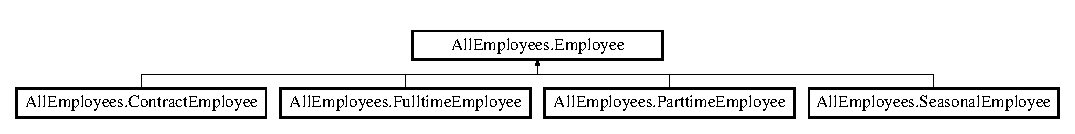
\includegraphics[height=1.352657cm]{class_all_employees_1_1_employee}
\end{center}
\end{figure}
\subsection*{Public Member Functions}
\begin{DoxyCompactItemize}
\item 
\hyperlink{class_all_employees_1_1_employee_ac3aa5a59bf1ddba2c45cc933bf897e04}{Employee} ()
\begin{DoxyCompactList}\small\item\em default constructor. Sets all values to default \end{DoxyCompactList}\item 
\hyperlink{class_all_employees_1_1_employee_a0a75e7e1786f2c6e5fa482ad79a99234}{Employee} (string first\+Name, string last\+Name)
\begin{DoxyCompactList}\small\item\em overloaded constructor. Sets name to inputed names, set all other values to default \end{DoxyCompactList}\item 
\hyperlink{class_all_employees_1_1_employee_aae0bb0d49eb93ff488771dca5a3db315}{Employee} (string first\+Name, string last\+Name, int social\+Insurance\+Number, Date\+Time date\+Of\+Birth, string employee\+Type)
\begin{DoxyCompactList}\small\item\em overloaded constructor. Sets all values to the values given. no default values \end{DoxyCompactList}\item 
bool \hyperlink{class_all_employees_1_1_employee_ad44ba8da1da1dceb64e1e6f9e6f7c5a3}{Set\+First\+Name} (string first\+Name)
\begin{DoxyCompactList}\small\item\em Setter for first\+Name. \end{DoxyCompactList}\item 
bool \hyperlink{class_all_employees_1_1_employee_a2b5ead1b4de39d2024422c4443034d4c}{Set\+Last\+Name} (string last\+Name)
\begin{DoxyCompactList}\small\item\em Setter for last\+Name. \end{DoxyCompactList}\item 
bool \hyperlink{class_all_employees_1_1_employee_a25c3c9fd99a595fb812b3ba6791f3f11}{Set\+Social\+Insurance\+Number} (int social\+Insurance\+Number)
\begin{DoxyCompactList}\small\item\em Setter for social\+Insurance\+Number. \end{DoxyCompactList}\item 
bool \hyperlink{class_all_employees_1_1_employee_a058b085f3c60bbe744bd10cc1f7a2bdb}{Set\+Date\+Of\+Birth} (Date\+Time date)
\begin{DoxyCompactList}\small\item\em Setter for date\+Of\+Birth using Date\+Time. \end{DoxyCompactList}\item 
bool \hyperlink{class_all_employees_1_1_employee_a66c163e386a335040a33a583d9d20d7c}{Set\+Date\+Of\+Birth} (string date)
\begin{DoxyCompactList}\small\item\em Setter for date\+Of\+Birth with String. \end{DoxyCompactList}\item 
bool \hyperlink{class_all_employees_1_1_employee_ac095c524a6b57edd0daea893c89874f5}{Set\+Date\+Of\+Birth} (int year, int month, int day)
\begin{DoxyCompactList}\small\item\em Setter for date\+Of\+Birth with ints. \end{DoxyCompactList}\item 
bool \hyperlink{class_all_employees_1_1_employee_aabdb35f9e42e4847bc33fda68482f7ab}{Set\+Employee\+Type} (string employee\+Type)
\begin{DoxyCompactList}\small\item\em Setter for type of employee. \end{DoxyCompactList}\item 
string \hyperlink{class_all_employees_1_1_employee_ae585e71d63222bcd0b87581fc8c1f936}{Get\+First\+Name} ()
\begin{DoxyCompactList}\small\item\em Getter for first\+Name. \end{DoxyCompactList}\item 
string \hyperlink{class_all_employees_1_1_employee_afaf5dbaa12c35930b36d3582e831b407}{Get\+Last\+Name} ()
\begin{DoxyCompactList}\small\item\em Getter for last\+Name. \end{DoxyCompactList}\item 
int \hyperlink{class_all_employees_1_1_employee_a0b5c62bd8eca3acd7f0921a478d8aefa}{Get\+Social\+Insurance\+Number} ()
\begin{DoxyCompactList}\small\item\em Getter for social\+Insurance\+Number. \end{DoxyCompactList}\item 
Date\+Time \hyperlink{class_all_employees_1_1_employee_a98f7200d68ab6a59f4e3283b8f81ce28}{Get\+Date\+Of\+Birth} ()
\begin{DoxyCompactList}\small\item\em Getter for date\+Of\+Birth. \end{DoxyCompactList}\item 
string \hyperlink{class_all_employees_1_1_employee_a2c310cf42cb87541a5fde6771e667212}{Get\+Date\+Of\+Birth\+String} ()
\begin{DoxyCompactList}\small\item\em Getter for date\+Of\+Birth that returns formatted string. \end{DoxyCompactList}\item 
string \hyperlink{class_all_employees_1_1_employee_a39116fe8a1dcc18735c92c1a3fcb579e}{Get\+Employee\+Type} ()
\begin{DoxyCompactList}\small\item\em Getter for employee\+Type. \end{DoxyCompactList}\end{DoxyCompactItemize}
\subsection*{Protected Member Functions}
\begin{DoxyCompactItemize}
\item 
bool \hyperlink{class_all_employees_1_1_employee_af679e8b4c683b9e94bec085062e5c88e}{Validate\+Base} ()
\begin{DoxyCompactList}\small\item\em Used to determine in the object contains a valid employee. \end{DoxyCompactList}\item 
string \hyperlink{class_all_employees_1_1_employee_a9e957826e327579e190cd5075789d1a9}{To\+String\+Base} ()
\begin{DoxyCompactList}\small\item\em Overriden method To\+String used to return a formated string of all data. \end{DoxyCompactList}\end{DoxyCompactItemize}
\subsection*{Private Attributes}
\begin{DoxyCompactItemize}
\item 
\hypertarget{class_all_employees_1_1_employee_a04c4c16015aa2d889fd2042ce4b8a1d7}{}string {\bfseries first\+Name}\label{class_all_employees_1_1_employee_a04c4c16015aa2d889fd2042ce4b8a1d7}

\item 
\hypertarget{class_all_employees_1_1_employee_ac3721b61919ca9cd29a400620562170e}{}string {\bfseries last\+Name}\label{class_all_employees_1_1_employee_ac3721b61919ca9cd29a400620562170e}

\item 
\hypertarget{class_all_employees_1_1_employee_a31f55bb91fe0871c5d9a3cb77f44a4df}{}int {\bfseries social\+Insurance\+Number}\label{class_all_employees_1_1_employee_a31f55bb91fe0871c5d9a3cb77f44a4df}

\item 
\hypertarget{class_all_employees_1_1_employee_a00f33298e4408f0a0402a34c9aa2067a}{}Date\+Time {\bfseries date\+Of\+Birth}\label{class_all_employees_1_1_employee_a00f33298e4408f0a0402a34c9aa2067a}

\item 
\hypertarget{class_all_employees_1_1_employee_a246198254823dc5a10197029b17479b4}{}string {\bfseries employee\+Type}\label{class_all_employees_1_1_employee_a246198254823dc5a10197029b17479b4}

\end{DoxyCompactItemize}


\subsection{Detailed Description}
{\bfseries Brief Description} The \hyperlink{class_all_employees_1_1_employee}{Employee} class is used to hold the basic infomation for all types of employees This class is the parent to many classes that furthur define different types of employees 

\begin{DoxyAuthor}{Author}
{\itshape Brandon} 
\end{DoxyAuthor}


\subsection{Constructor \& Destructor Documentation}
\hypertarget{class_all_employees_1_1_employee_ac3aa5a59bf1ddba2c45cc933bf897e04}{}\index{All\+Employees\+::\+Employee@{All\+Employees\+::\+Employee}!Employee@{Employee}}
\index{Employee@{Employee}!All\+Employees\+::\+Employee@{All\+Employees\+::\+Employee}}
\subsubsection[{Employee}]{\setlength{\rightskip}{0pt plus 5cm}All\+Employees.\+Employee.\+Employee (
\begin{DoxyParamCaption}
{}
\end{DoxyParamCaption}
)}\label{class_all_employees_1_1_employee_ac3aa5a59bf1ddba2c45cc933bf897e04}


default constructor. Sets all values to default 

{\bfseries Details}


\begin{DoxyParams}{Parameters}
{\em n/a} & \\
\hline
\end{DoxyParams}
\begin{DoxyReturn}{Returns}
n/a 
\end{DoxyReturn}
\hypertarget{class_all_employees_1_1_employee_a0a75e7e1786f2c6e5fa482ad79a99234}{}\index{All\+Employees\+::\+Employee@{All\+Employees\+::\+Employee}!Employee@{Employee}}
\index{Employee@{Employee}!All\+Employees\+::\+Employee@{All\+Employees\+::\+Employee}}
\subsubsection[{Employee}]{\setlength{\rightskip}{0pt plus 5cm}All\+Employees.\+Employee.\+Employee (
\begin{DoxyParamCaption}
\item[{string}]{first\+Name, }
\item[{string}]{last\+Name}
\end{DoxyParamCaption}
)}\label{class_all_employees_1_1_employee_a0a75e7e1786f2c6e5fa482ad79a99234}


overloaded constructor. Sets name to inputed names, set all other values to default 

{\bfseries Details}


\begin{DoxyParams}{Parameters}
{\em first\+Name} & -\/ {\bfseries string} -\/ First Name of employee to add to records \\
\hline
{\em last\+Name} & -\/ {\bfseries string} -\/ Last Name of employee to add to records\\
\hline
\end{DoxyParams}

\begin{DoxyExceptions}{Exceptions}
{\em $<$\+Failed\+Constructor\+Exception$>$} & -\/ If the constructor failed to create the object\\
\hline
\end{DoxyExceptions}
\begin{DoxyReturn}{Returns}
n/a 
\end{DoxyReturn}
\hypertarget{class_all_employees_1_1_employee_aae0bb0d49eb93ff488771dca5a3db315}{}\index{All\+Employees\+::\+Employee@{All\+Employees\+::\+Employee}!Employee@{Employee}}
\index{Employee@{Employee}!All\+Employees\+::\+Employee@{All\+Employees\+::\+Employee}}
\subsubsection[{Employee}]{\setlength{\rightskip}{0pt plus 5cm}All\+Employees.\+Employee.\+Employee (
\begin{DoxyParamCaption}
\item[{string}]{first\+Name, }
\item[{string}]{last\+Name, }
\item[{int}]{social\+Insurance\+Number, }
\item[{Date\+Time}]{date\+Of\+Birth, }
\item[{string}]{employee\+Type}
\end{DoxyParamCaption}
)}\label{class_all_employees_1_1_employee_aae0bb0d49eb93ff488771dca5a3db315}


overloaded constructor. Sets all values to the values given. no default values 

{\bfseries Details}


\begin{DoxyParams}{Parameters}
{\em first\+Name} & -\/ {\bfseries string} -\/ First Name of employee to add to records \\
\hline
{\em last\+Name} & -\/ {\bfseries string} -\/ Last Name of employee to add to records \\
\hline
{\em social\+Insurance\+Number} & -\/ {\bfseries int} -\/ Social Insurance Number of employee to add to records \\
\hline
{\em date\+Of\+Birth} & -\/ {\bfseries Date\+Time} -\/ Date Of Birth of employee to add to records\\
\hline
\end{DoxyParams}

\begin{DoxyExceptions}{Exceptions}
{\em $<$\+Failed\+Constructor\+Exception$>$} & -\/ If the constructor failed to create the object\\
\hline
\end{DoxyExceptions}
\begin{DoxyReturn}{Returns}
n/a 
\end{DoxyReturn}


\subsection{Member Function Documentation}
\hypertarget{class_all_employees_1_1_employee_a98f7200d68ab6a59f4e3283b8f81ce28}{}\index{All\+Employees\+::\+Employee@{All\+Employees\+::\+Employee}!Get\+Date\+Of\+Birth@{Get\+Date\+Of\+Birth}}
\index{Get\+Date\+Of\+Birth@{Get\+Date\+Of\+Birth}!All\+Employees\+::\+Employee@{All\+Employees\+::\+Employee}}
\subsubsection[{Get\+Date\+Of\+Birth}]{\setlength{\rightskip}{0pt plus 5cm}Date\+Time All\+Employees.\+Employee.\+Get\+Date\+Of\+Birth (
\begin{DoxyParamCaption}
{}
\end{DoxyParamCaption}
)}\label{class_all_employees_1_1_employee_a98f7200d68ab6a59f4e3283b8f81ce28}


Getter for date\+Of\+Birth. 

{\bfseries Details}


\begin{DoxyParams}{Parameters}
{\em n/a} & \\
\hline
\end{DoxyParams}
\begin{DoxyReturn}{Returns}
date\+Of\+Birth {\bfseries string} 
\end{DoxyReturn}
\hypertarget{class_all_employees_1_1_employee_a2c310cf42cb87541a5fde6771e667212}{}\index{All\+Employees\+::\+Employee@{All\+Employees\+::\+Employee}!Get\+Date\+Of\+Birth\+String@{Get\+Date\+Of\+Birth\+String}}
\index{Get\+Date\+Of\+Birth\+String@{Get\+Date\+Of\+Birth\+String}!All\+Employees\+::\+Employee@{All\+Employees\+::\+Employee}}
\subsubsection[{Get\+Date\+Of\+Birth\+String}]{\setlength{\rightskip}{0pt plus 5cm}string All\+Employees.\+Employee.\+Get\+Date\+Of\+Birth\+String (
\begin{DoxyParamCaption}
{}
\end{DoxyParamCaption}
)}\label{class_all_employees_1_1_employee_a2c310cf42cb87541a5fde6771e667212}


Getter for date\+Of\+Birth that returns formatted string. 

{\bfseries Details}


\begin{DoxyParams}{Parameters}
{\em n/a} & \\
\hline
\end{DoxyParams}
\begin{DoxyReturn}{Returns}
date\+Of\+Birth {\bfseries string} 
\end{DoxyReturn}
\hypertarget{class_all_employees_1_1_employee_a39116fe8a1dcc18735c92c1a3fcb579e}{}\index{All\+Employees\+::\+Employee@{All\+Employees\+::\+Employee}!Get\+Employee\+Type@{Get\+Employee\+Type}}
\index{Get\+Employee\+Type@{Get\+Employee\+Type}!All\+Employees\+::\+Employee@{All\+Employees\+::\+Employee}}
\subsubsection[{Get\+Employee\+Type}]{\setlength{\rightskip}{0pt plus 5cm}string All\+Employees.\+Employee.\+Get\+Employee\+Type (
\begin{DoxyParamCaption}
{}
\end{DoxyParamCaption}
)}\label{class_all_employees_1_1_employee_a39116fe8a1dcc18735c92c1a3fcb579e}


Getter for employee\+Type. 

{\bfseries Details}


\begin{DoxyParams}{Parameters}
{\em n/a} & \\
\hline
\end{DoxyParams}
\begin{DoxyReturn}{Returns}
employee\+Type {\bfseries string} 
\end{DoxyReturn}
\hypertarget{class_all_employees_1_1_employee_ae585e71d63222bcd0b87581fc8c1f936}{}\index{All\+Employees\+::\+Employee@{All\+Employees\+::\+Employee}!Get\+First\+Name@{Get\+First\+Name}}
\index{Get\+First\+Name@{Get\+First\+Name}!All\+Employees\+::\+Employee@{All\+Employees\+::\+Employee}}
\subsubsection[{Get\+First\+Name}]{\setlength{\rightskip}{0pt plus 5cm}string All\+Employees.\+Employee.\+Get\+First\+Name (
\begin{DoxyParamCaption}
{}
\end{DoxyParamCaption}
)}\label{class_all_employees_1_1_employee_ae585e71d63222bcd0b87581fc8c1f936}


Getter for first\+Name. 

{\bfseries Details}


\begin{DoxyParams}{Parameters}
{\em n/a} & \\
\hline
\end{DoxyParams}
\begin{DoxyReturn}{Returns}
first\+Name {\bfseries string} 
\end{DoxyReturn}
\hypertarget{class_all_employees_1_1_employee_afaf5dbaa12c35930b36d3582e831b407}{}\index{All\+Employees\+::\+Employee@{All\+Employees\+::\+Employee}!Get\+Last\+Name@{Get\+Last\+Name}}
\index{Get\+Last\+Name@{Get\+Last\+Name}!All\+Employees\+::\+Employee@{All\+Employees\+::\+Employee}}
\subsubsection[{Get\+Last\+Name}]{\setlength{\rightskip}{0pt plus 5cm}string All\+Employees.\+Employee.\+Get\+Last\+Name (
\begin{DoxyParamCaption}
{}
\end{DoxyParamCaption}
)}\label{class_all_employees_1_1_employee_afaf5dbaa12c35930b36d3582e831b407}


Getter for last\+Name. 

{\bfseries Details}


\begin{DoxyParams}{Parameters}
{\em n/a} & \\
\hline
\end{DoxyParams}
\begin{DoxyReturn}{Returns}
last\+Name {\bfseries string} 
\end{DoxyReturn}
\hypertarget{class_all_employees_1_1_employee_a0b5c62bd8eca3acd7f0921a478d8aefa}{}\index{All\+Employees\+::\+Employee@{All\+Employees\+::\+Employee}!Get\+Social\+Insurance\+Number@{Get\+Social\+Insurance\+Number}}
\index{Get\+Social\+Insurance\+Number@{Get\+Social\+Insurance\+Number}!All\+Employees\+::\+Employee@{All\+Employees\+::\+Employee}}
\subsubsection[{Get\+Social\+Insurance\+Number}]{\setlength{\rightskip}{0pt plus 5cm}int All\+Employees.\+Employee.\+Get\+Social\+Insurance\+Number (
\begin{DoxyParamCaption}
{}
\end{DoxyParamCaption}
)}\label{class_all_employees_1_1_employee_a0b5c62bd8eca3acd7f0921a478d8aefa}


Getter for social\+Insurance\+Number. 

{\bfseries Details}


\begin{DoxyParams}{Parameters}
{\em n/a} & \\
\hline
\end{DoxyParams}
\begin{DoxyReturn}{Returns}
social\+Insurance\+Number {\bfseries int} 
\end{DoxyReturn}
\hypertarget{class_all_employees_1_1_employee_a058b085f3c60bbe744bd10cc1f7a2bdb}{}\index{All\+Employees\+::\+Employee@{All\+Employees\+::\+Employee}!Set\+Date\+Of\+Birth@{Set\+Date\+Of\+Birth}}
\index{Set\+Date\+Of\+Birth@{Set\+Date\+Of\+Birth}!All\+Employees\+::\+Employee@{All\+Employees\+::\+Employee}}
\subsubsection[{Set\+Date\+Of\+Birth}]{\setlength{\rightskip}{0pt plus 5cm}bool All\+Employees.\+Employee.\+Set\+Date\+Of\+Birth (
\begin{DoxyParamCaption}
\item[{Date\+Time}]{date}
\end{DoxyParamCaption}
)}\label{class_all_employees_1_1_employee_a058b085f3c60bbe744bd10cc1f7a2bdb}


Setter for date\+Of\+Birth using Date\+Time. 

{\bfseries Details}


\begin{DoxyParams}{Parameters}
{\em date} & {\bfseries Date\+Time} -\/ The date of birth of the employee\\
\hline
\end{DoxyParams}
\begin{DoxyReturn}{Returns}
data\+Saved {\bfseries bool} -\/ true if input was valid and data was changed. False it data was not changed 
\end{DoxyReturn}
\hypertarget{class_all_employees_1_1_employee_a66c163e386a335040a33a583d9d20d7c}{}\index{All\+Employees\+::\+Employee@{All\+Employees\+::\+Employee}!Set\+Date\+Of\+Birth@{Set\+Date\+Of\+Birth}}
\index{Set\+Date\+Of\+Birth@{Set\+Date\+Of\+Birth}!All\+Employees\+::\+Employee@{All\+Employees\+::\+Employee}}
\subsubsection[{Set\+Date\+Of\+Birth}]{\setlength{\rightskip}{0pt plus 5cm}bool All\+Employees.\+Employee.\+Set\+Date\+Of\+Birth (
\begin{DoxyParamCaption}
\item[{string}]{date}
\end{DoxyParamCaption}
)}\label{class_all_employees_1_1_employee_a66c163e386a335040a33a583d9d20d7c}


Setter for date\+Of\+Birth with String. 

{\bfseries Details}


\begin{DoxyParams}{Parameters}
{\em date} & {\bfseries string} -\/ The date of birth of the employee\\
\hline
\end{DoxyParams}
\begin{DoxyReturn}{Returns}
data\+Saved {\bfseries bool} -\/ true if input was valid and data was changed. False it data was not changed 
\end{DoxyReturn}
\hypertarget{class_all_employees_1_1_employee_ac095c524a6b57edd0daea893c89874f5}{}\index{All\+Employees\+::\+Employee@{All\+Employees\+::\+Employee}!Set\+Date\+Of\+Birth@{Set\+Date\+Of\+Birth}}
\index{Set\+Date\+Of\+Birth@{Set\+Date\+Of\+Birth}!All\+Employees\+::\+Employee@{All\+Employees\+::\+Employee}}
\subsubsection[{Set\+Date\+Of\+Birth}]{\setlength{\rightskip}{0pt plus 5cm}bool All\+Employees.\+Employee.\+Set\+Date\+Of\+Birth (
\begin{DoxyParamCaption}
\item[{int}]{year, }
\item[{int}]{month, }
\item[{int}]{day}
\end{DoxyParamCaption}
)}\label{class_all_employees_1_1_employee_ac095c524a6b57edd0daea893c89874f5}


Setter for date\+Of\+Birth with ints. 

{\bfseries Details}


\begin{DoxyParams}{Parameters}
{\em year} & {\bfseries int} -\/ The year of birth of the employee \\
\hline
{\em month} & {\bfseries int} -\/ The month of birth of the employee \\
\hline
{\em day} & {\bfseries int} -\/ The day of birth of the employee\\
\hline
\end{DoxyParams}
\begin{DoxyReturn}{Returns}
data\+Saved {\bfseries bool} -\/ true if input was valid and data was changed. False it data was not changed 
\end{DoxyReturn}
\hypertarget{class_all_employees_1_1_employee_aabdb35f9e42e4847bc33fda68482f7ab}{}\index{All\+Employees\+::\+Employee@{All\+Employees\+::\+Employee}!Set\+Employee\+Type@{Set\+Employee\+Type}}
\index{Set\+Employee\+Type@{Set\+Employee\+Type}!All\+Employees\+::\+Employee@{All\+Employees\+::\+Employee}}
\subsubsection[{Set\+Employee\+Type}]{\setlength{\rightskip}{0pt plus 5cm}bool All\+Employees.\+Employee.\+Set\+Employee\+Type (
\begin{DoxyParamCaption}
\item[{string}]{employee\+Type}
\end{DoxyParamCaption}
)}\label{class_all_employees_1_1_employee_aabdb35f9e42e4847bc33fda68482f7ab}


Setter for type of employee. 

{\bfseries Details}


\begin{DoxyParams}{Parameters}
{\em employee\+Type} & {\bfseries string} -\/ The type of the employee. Must be\+: \char`\"{}\+F\+T\char`\"{} \char`\"{}\+P\+T\char`\"{} \char`\"{}\+C\+T\char`\"{} \char`\"{}\+S\+N\char`\"{} or \char`\"{}\char`\"{}\\
\hline
\end{DoxyParams}
\begin{DoxyReturn}{Returns}
data\+Saved {\bfseries bool} -\/ true if input was valid and data was changed. False it data was not changed 
\end{DoxyReturn}
\hypertarget{class_all_employees_1_1_employee_ad44ba8da1da1dceb64e1e6f9e6f7c5a3}{}\index{All\+Employees\+::\+Employee@{All\+Employees\+::\+Employee}!Set\+First\+Name@{Set\+First\+Name}}
\index{Set\+First\+Name@{Set\+First\+Name}!All\+Employees\+::\+Employee@{All\+Employees\+::\+Employee}}
\subsubsection[{Set\+First\+Name}]{\setlength{\rightskip}{0pt plus 5cm}bool All\+Employees.\+Employee.\+Set\+First\+Name (
\begin{DoxyParamCaption}
\item[{string}]{first\+Name}
\end{DoxyParamCaption}
)}\label{class_all_employees_1_1_employee_ad44ba8da1da1dceb64e1e6f9e6f7c5a3}


Setter for first\+Name. 

{\bfseries Details}


\begin{DoxyParams}{Parameters}
{\em first\+Name} & {\bfseries string} -\/ The first name of the employee\\
\hline
\end{DoxyParams}
\begin{DoxyReturn}{Returns}
data\+Saved {\bfseries bool} -\/ true if input was valid and data was changed. False it data was not changed 
\end{DoxyReturn}
\hypertarget{class_all_employees_1_1_employee_a2b5ead1b4de39d2024422c4443034d4c}{}\index{All\+Employees\+::\+Employee@{All\+Employees\+::\+Employee}!Set\+Last\+Name@{Set\+Last\+Name}}
\index{Set\+Last\+Name@{Set\+Last\+Name}!All\+Employees\+::\+Employee@{All\+Employees\+::\+Employee}}
\subsubsection[{Set\+Last\+Name}]{\setlength{\rightskip}{0pt plus 5cm}bool All\+Employees.\+Employee.\+Set\+Last\+Name (
\begin{DoxyParamCaption}
\item[{string}]{last\+Name}
\end{DoxyParamCaption}
)}\label{class_all_employees_1_1_employee_a2b5ead1b4de39d2024422c4443034d4c}


Setter for last\+Name. 

{\bfseries Details}


\begin{DoxyParams}{Parameters}
{\em lastt\+Name} & {\bfseries string} -\/ The last name of the employee\\
\hline
\end{DoxyParams}
\begin{DoxyReturn}{Returns}
data\+Saved {\bfseries bool} -\/ true if input was valid and data was changed. False it data was not changed 
\end{DoxyReturn}
\hypertarget{class_all_employees_1_1_employee_a25c3c9fd99a595fb812b3ba6791f3f11}{}\index{All\+Employees\+::\+Employee@{All\+Employees\+::\+Employee}!Set\+Social\+Insurance\+Number@{Set\+Social\+Insurance\+Number}}
\index{Set\+Social\+Insurance\+Number@{Set\+Social\+Insurance\+Number}!All\+Employees\+::\+Employee@{All\+Employees\+::\+Employee}}
\subsubsection[{Set\+Social\+Insurance\+Number}]{\setlength{\rightskip}{0pt plus 5cm}bool All\+Employees.\+Employee.\+Set\+Social\+Insurance\+Number (
\begin{DoxyParamCaption}
\item[{int}]{social\+Insurance\+Number}
\end{DoxyParamCaption}
)}\label{class_all_employees_1_1_employee_a25c3c9fd99a595fb812b3ba6791f3f11}


Setter for social\+Insurance\+Number. 

{\bfseries Details}


\begin{DoxyParams}{Parameters}
{\em social\+Insurance\+Number} & {\bfseries int} -\/ The social insurance number of the employee\\
\hline
\end{DoxyParams}
\begin{DoxyReturn}{Returns}
data\+Saved {\bfseries bool} -\/ true if input was valid and data was changed. False it data was not changed 
\end{DoxyReturn}
\hypertarget{class_all_employees_1_1_employee_a9e957826e327579e190cd5075789d1a9}{}\index{All\+Employees\+::\+Employee@{All\+Employees\+::\+Employee}!To\+String\+Base@{To\+String\+Base}}
\index{To\+String\+Base@{To\+String\+Base}!All\+Employees\+::\+Employee@{All\+Employees\+::\+Employee}}
\subsubsection[{To\+String\+Base}]{\setlength{\rightskip}{0pt plus 5cm}string All\+Employees.\+Employee.\+To\+String\+Base (
\begin{DoxyParamCaption}
{}
\end{DoxyParamCaption}
)\hspace{0.3cm}{\ttfamily [protected]}}\label{class_all_employees_1_1_employee_a9e957826e327579e190cd5075789d1a9}


Overriden method To\+String used to return a formated string of all data. 

{\bfseries Details}


\begin{DoxyParams}{Parameters}
{\em n/a} & \\
\hline
\end{DoxyParams}
\begin{DoxyReturn}{Returns}
employee\+String {\bfseries string} -\/ the formated string containing all employee data 
\end{DoxyReturn}
\hypertarget{class_all_employees_1_1_employee_af679e8b4c683b9e94bec085062e5c88e}{}\index{All\+Employees\+::\+Employee@{All\+Employees\+::\+Employee}!Validate\+Base@{Validate\+Base}}
\index{Validate\+Base@{Validate\+Base}!All\+Employees\+::\+Employee@{All\+Employees\+::\+Employee}}
\subsubsection[{Validate\+Base}]{\setlength{\rightskip}{0pt plus 5cm}bool All\+Employees.\+Employee.\+Validate\+Base (
\begin{DoxyParamCaption}
{}
\end{DoxyParamCaption}
)\hspace{0.3cm}{\ttfamily [protected]}}\label{class_all_employees_1_1_employee_af679e8b4c683b9e94bec085062e5c88e}


Used to determine in the object contains a valid employee. 

{\bfseries Details}


\begin{DoxyParams}{Parameters}
{\em n/a} & \\
\hline
\end{DoxyParams}
\begin{DoxyReturn}{Returns}
data\+Valid -\/ {\bfseries bool} -\/ True if the object contains all data for a valid employee 
\end{DoxyReturn}


The documentation for this class was generated from the following file\+:\begin{DoxyCompactItemize}
\item 
C\+:/\+S\+E\+T\+Repo/trunk/\+E\+M\+S/trunk/\+All\+Employees/\+All\+Employees/Employee.\+cs\end{DoxyCompactItemize}

\hypertarget{class_my_all_employee_1_1_tests_1_1_employee_tests}{}\section{My\+All\+Employee.\+Tests.\+Employee\+Tests Class Reference}
\label{class_my_all_employee_1_1_tests_1_1_employee_tests}\index{My\+All\+Employee.\+Tests.\+Employee\+Tests@{My\+All\+Employee.\+Tests.\+Employee\+Tests}}
\subsection*{Public Member Functions}
\begin{DoxyCompactItemize}
\item 
void \hyperlink{class_my_all_employee_1_1_tests_1_1_employee_tests_a610698076f207b59950425f3a1c0574e}{Constructor\+With\+Names\+Test\+Valid1} ()
\begin{DoxyCompactList}\small\item\em This unit test will check if either name contains anything other than a letter, apostrophe, dash. It will throw an exception if wrong. \end{DoxyCompactList}\item 
void \hyperlink{class_my_all_employee_1_1_tests_1_1_employee_tests_abcf2093b93345bfd9225403f5fc85ad0}{Constructor\+With\+Names\+Test\+Valid2} ()
\begin{DoxyCompactList}\small\item\em This unit test will check if either name contains anything other than a letter, apostrophe, dash. It will throw an exception if wrong. \end{DoxyCompactList}\item 
void \hyperlink{class_my_all_employee_1_1_tests_1_1_employee_tests_a569d10ab841a21609fa5296650ad6f0d}{Constructor\+With\+Names\+Test\+Valid3} ()
\begin{DoxyCompactList}\small\item\em This unit test will check if either name contains anything other than a letter, apostrophe, dash. It will throw an exception if wrong. \end{DoxyCompactList}\item 
void \hyperlink{class_my_all_employee_1_1_tests_1_1_employee_tests_aa12327a24a378d606e2aa2b95c523cd5}{Constructor\+With\+Names\+Test\+Invalid\+Slash} ()
\begin{DoxyCompactList}\small\item\em This unit test will check if the constructor will fail and if the string is invalid because it contains a slash. \end{DoxyCompactList}\item 
void \hyperlink{class_my_all_employee_1_1_tests_1_1_employee_tests_a631ee75ab21985aba7c38247a0bb3f2e}{Constructor\+With\+Names\+Test\+Invalid\+Space} ()
\begin{DoxyCompactList}\small\item\em This unit test will check if the constructor will fail and if the string is invalid because it contains a space. \end{DoxyCompactList}\item 
void \hyperlink{class_my_all_employee_1_1_tests_1_1_employee_tests_a2f4da21d02d8e126a72d869a2af7f56c}{Constructor\+With\+Names\+Test\+Invalid\+Number} ()
\begin{DoxyCompactList}\small\item\em This unit test will check if the constructor will fail and if the string is invalid because it contains a number. \end{DoxyCompactList}\item 
void \hyperlink{class_my_all_employee_1_1_tests_1_1_employee_tests_a7890c0db13ca221a80eddfb68861eee5}{Constructor\+With\+All\+Param\+Test\+Valid1} ()
\begin{DoxyCompactList}\small\item\em This unit test will check the constructor that takes in all possible parameters, and give them all valid data. \end{DoxyCompactList}\item 
void \hyperlink{class_my_all_employee_1_1_tests_1_1_employee_tests_acb3a7727aeb8ed45f0fcd462233afd34}{Constructor\+With\+All\+Param\+Test\+Valid2} ()
\begin{DoxyCompactList}\small\item\em This unit test will check the constructor that takes in all possible parameters, and give them all valid data. \end{DoxyCompactList}\item 
void \hyperlink{class_my_all_employee_1_1_tests_1_1_employee_tests_af07472233dc8fafad82d768d8cd55571}{Constructor\+With\+All\+Param\+Test\+Valid3} ()
\begin{DoxyCompactList}\small\item\em This unit test will check the constructor that takes in all possible parameters, and give them all valid data. \end{DoxyCompactList}\item 
void \hyperlink{class_my_all_employee_1_1_tests_1_1_employee_tests_ad15721c3192881537aabecfe234d4e97}{Constructor\+With\+All\+Param\+Test\+Invalid\+S\+I\+N} ()
\begin{DoxyCompactList}\small\item\em This unit test will check the constructor that takes in all possible parameters, and give them all invalid data. \end{DoxyCompactList}\item 
void \hyperlink{class_my_all_employee_1_1_tests_1_1_employee_tests_ae23b307e9a25395d912d35dfd528a425}{Constructor\+With\+All\+Param\+Test\+Invalid\+Employee\+Type} ()
\begin{DoxyCompactList}\small\item\em This unit test will check the constructor that takes in all possible parameters, and give them all invalid data. \end{DoxyCompactList}\item 
void \hyperlink{class_my_all_employee_1_1_tests_1_1_employee_tests_ad1b7c619af913a7432cd0fee38780e79}{Constructor\+With\+All\+Param\+Test\+Invalid\+First\+Name} ()
\begin{DoxyCompactList}\small\item\em This unit test will check the constructor that takes in all possible parameters, and give them all invalid data. \end{DoxyCompactList}\item 
void \hyperlink{class_my_all_employee_1_1_tests_1_1_employee_tests_a3bfac4379a4a632f9e7dd2a5069e3f6b}{Set\+First\+Name\+Test\+Valid1} ()
\begin{DoxyCompactList}\small\item\em This unit test will set the first name to a valid value. \end{DoxyCompactList}\item 
void \hyperlink{class_my_all_employee_1_1_tests_1_1_employee_tests_a435bffb5dabc53bf457a5af13ad0bef4}{Set\+First\+Name\+Test\+Valid2} ()
\begin{DoxyCompactList}\small\item\em This unit test will set the first name to a valid value. \end{DoxyCompactList}\item 
void \hyperlink{class_my_all_employee_1_1_tests_1_1_employee_tests_afb579cc0ea6380dceddc7935bd5a058d}{Set\+First\+Name\+Test\+Valid3} ()
\begin{DoxyCompactList}\small\item\em This unit test will set the first name to a valid value. \end{DoxyCompactList}\item 
void \hyperlink{class_my_all_employee_1_1_tests_1_1_employee_tests_acf02476171850b945471ac3b53c73ef3}{Set\+First\+Name\+Test\+Invalid\+Space} ()
\begin{DoxyCompactList}\small\item\em This unit test will set the first name to an invalid value. \end{DoxyCompactList}\item 
void \hyperlink{class_my_all_employee_1_1_tests_1_1_employee_tests_a12e807fb2fd6888b20572f246c692651}{Set\+First\+Name\+Test\+Invalid\+Number} ()
\begin{DoxyCompactList}\small\item\em This unit test will set the first name to an invalid value. \end{DoxyCompactList}\item 
void \hyperlink{class_my_all_employee_1_1_tests_1_1_employee_tests_ab18a4774eeb60fff1f2ab3ef420e0f9a}{Set\+First\+Name\+Test\+Invalid\+Slash} ()
\begin{DoxyCompactList}\small\item\em This unit test will set the first name to an invalid value. \end{DoxyCompactList}\item 
void \hyperlink{class_my_all_employee_1_1_tests_1_1_employee_tests_a382b99f0206a268573ba0533c6ed0f68}{Set\+Last\+Name\+Test\+Valid1} ()
\begin{DoxyCompactList}\small\item\em This unit test will set the last name to a valid value. \end{DoxyCompactList}\item 
void \hyperlink{class_my_all_employee_1_1_tests_1_1_employee_tests_a45e549be691bb05aac84850f00265482}{Set\+Last\+Name\+Test\+Valid2} ()
\begin{DoxyCompactList}\small\item\em This unit test will set the last name to a valid value. \end{DoxyCompactList}\item 
void \hyperlink{class_my_all_employee_1_1_tests_1_1_employee_tests_a112321d5dc92bc7d995625c94e0bb376}{Set\+Last\+Name\+Test\+Valid3} ()
\begin{DoxyCompactList}\small\item\em This unit test will set the last name to a valid value. \end{DoxyCompactList}\item 
void \hyperlink{class_my_all_employee_1_1_tests_1_1_employee_tests_a958f22718abef1aef9a6579c6a6b6f53}{Set\+Last\+Name\+Test\+Invalid\+Space} ()
\begin{DoxyCompactList}\small\item\em This unit test will set the last name to an invalid value. \end{DoxyCompactList}\item 
void \hyperlink{class_my_all_employee_1_1_tests_1_1_employee_tests_a30f22d9b4911bf2d1b8c489415bcd131}{Set\+Last\+Name\+Test\+Invalid\+Number} ()
\begin{DoxyCompactList}\small\item\em This unit test will set the last name to an invalid value. \end{DoxyCompactList}\item 
void \hyperlink{class_my_all_employee_1_1_tests_1_1_employee_tests_a6e548af8211151455c40c7a20756b9b1}{Set\+Last\+Name\+Test\+Invalid\+Slash} ()
\begin{DoxyCompactList}\small\item\em This unit test will set the last name to an invalid value. \end{DoxyCompactList}\item 
void \hyperlink{class_my_all_employee_1_1_tests_1_1_employee_tests_a3b5dae6ba3605c07bf85753fba24ce3e}{Set\+Social\+Insurance\+Number\+Test\+Valid} ()
\begin{DoxyCompactList}\small\item\em This unit test will set the S\+I\+N number to a valid number \textbackslash{} {\bfseries  Name of Method} \hyperlink{class_my_all_employee_1_1_tests_1_1_employee_tests_a3b5dae6ba3605c07bf85753fba24ce3e}{Set\+Social\+Insurance\+Number\+Test\+Valid()} \end{DoxyCompactList}\item 
void \hyperlink{class_my_all_employee_1_1_tests_1_1_employee_tests_aa7fed107bfc06f9e2e2e11767b1d2c07}{Set\+Social\+Insurance\+Number\+Test\+Invalid\+To\+Short} ()
\begin{DoxyCompactList}\small\item\em This unit test will set the S\+I\+N number to an invalid number \textbackslash{} {\bfseries  Name of Method} \hyperlink{class_my_all_employee_1_1_tests_1_1_employee_tests_aa7fed107bfc06f9e2e2e11767b1d2c07}{Set\+Social\+Insurance\+Number\+Test\+Invalid\+To\+Short()} \end{DoxyCompactList}\item 
void \hyperlink{class_my_all_employee_1_1_tests_1_1_employee_tests_ab7c711e3bd0579655e6a96a395cfd19e}{Set\+Social\+Insurance\+Number\+Test\+Invalid\+Negitive} ()
\begin{DoxyCompactList}\small\item\em This unit test will set the S\+I\+N number to an invalid number \textbackslash{} {\bfseries  Name of Method} \hyperlink{class_my_all_employee_1_1_tests_1_1_employee_tests_ab7c711e3bd0579655e6a96a395cfd19e}{Set\+Social\+Insurance\+Number\+Test\+Invalid\+Negitive()} \end{DoxyCompactList}\item 
void \hyperlink{class_my_all_employee_1_1_tests_1_1_employee_tests_a45dfe5f9e4be553bf514505e700221c3}{Set\+Social\+Insurance\+Number\+Test\+Invalid\+Too\+Large} ()
\begin{DoxyCompactList}\small\item\em This unit test will set the S\+I\+N number to an invalid number \textbackslash{} {\bfseries  Name of Method} \hyperlink{class_my_all_employee_1_1_tests_1_1_employee_tests_a45dfe5f9e4be553bf514505e700221c3}{Set\+Social\+Insurance\+Number\+Test\+Invalid\+Too\+Large()} \end{DoxyCompactList}\item 
void \hyperlink{class_my_all_employee_1_1_tests_1_1_employee_tests_adb92917123aa50123ed0198ebad41327}{Set\+Employee\+Type\+Test\+Valid\+Contract} ()
\begin{DoxyCompactList}\small\item\em This unit test will set the employee type to a valid value. \end{DoxyCompactList}\item 
void \hyperlink{class_my_all_employee_1_1_tests_1_1_employee_tests_a826c7c75c5ae1d95ab50b205a88a7553}{Set\+Employee\+Type\+Test\+Valid\+Full\+Time} ()
\begin{DoxyCompactList}\small\item\em This unit test will set the employee type to a valid value. \end{DoxyCompactList}\item 
void \hyperlink{class_my_all_employee_1_1_tests_1_1_employee_tests_a05c6b8130dc01a9a393ba0459bfb1662}{Set\+Employee\+Type\+Test\+Valid\+Part\+Time} ()
\begin{DoxyCompactList}\small\item\em This unit test will set the employee type to a valid value. \end{DoxyCompactList}\item 
void \hyperlink{class_my_all_employee_1_1_tests_1_1_employee_tests_a1c51363de67faf0cae1ace7a70afe294}{Set\+Employee\+Type\+Test\+Valid\+Seasonal} ()
\begin{DoxyCompactList}\small\item\em This unit test will set the employee type to a valid value. \end{DoxyCompactList}\item 
void \hyperlink{class_my_all_employee_1_1_tests_1_1_employee_tests_abd1fccba15048484dff6f4b08adbc2c6}{Set\+Employee\+Type\+Test\+Valid\+No\+Type} ()
\begin{DoxyCompactList}\small\item\em This unit test will set the employee type to a valid value. \end{DoxyCompactList}\item 
void \hyperlink{class_my_all_employee_1_1_tests_1_1_employee_tests_a5c9bfc38b7f20d1d08cc1cac7557fd38}{Set\+Employee\+Type\+Test\+Invalid} ()
\begin{DoxyCompactList}\small\item\em This unit test will set the employee type to an invalid value \textbackslash{} {\bfseries  Name of Method} \hyperlink{class_my_all_employee_1_1_tests_1_1_employee_tests_a5c9bfc38b7f20d1d08cc1cac7557fd38}{Set\+Employee\+Type\+Test\+Invalid()} \end{DoxyCompactList}\end{DoxyCompactItemize}


\subsection{Member Function Documentation}
\hypertarget{class_my_all_employee_1_1_tests_1_1_employee_tests_ae23b307e9a25395d912d35dfd528a425}{}\index{My\+All\+Employee\+::\+Tests\+::\+Employee\+Tests@{My\+All\+Employee\+::\+Tests\+::\+Employee\+Tests}!Constructor\+With\+All\+Param\+Test\+Invalid\+Employee\+Type@{Constructor\+With\+All\+Param\+Test\+Invalid\+Employee\+Type}}
\index{Constructor\+With\+All\+Param\+Test\+Invalid\+Employee\+Type@{Constructor\+With\+All\+Param\+Test\+Invalid\+Employee\+Type}!My\+All\+Employee\+::\+Tests\+::\+Employee\+Tests@{My\+All\+Employee\+::\+Tests\+::\+Employee\+Tests}}
\subsubsection[{Constructor\+With\+All\+Param\+Test\+Invalid\+Employee\+Type}]{\setlength{\rightskip}{0pt plus 5cm}void My\+All\+Employee.\+Tests.\+Employee\+Tests.\+Constructor\+With\+All\+Param\+Test\+Invalid\+Employee\+Type (
\begin{DoxyParamCaption}
{}
\end{DoxyParamCaption}
)}\label{class_my_all_employee_1_1_tests_1_1_employee_tests_ae23b307e9a25395d912d35dfd528a425}


This unit test will check the constructor that takes in all possible parameters, and give them all invalid data. 

\textbackslash{} {\bfseries  Name of Method} \hyperlink{class_my_all_employee_1_1_tests_1_1_employee_tests_ae23b307e9a25395d912d35dfd528a425}{Constructor\+With\+All\+Param\+Test\+Invalid\+Employee\+Type()}

\textbackslash{} {\bfseries  How test is Conducted} This test is run automatically

\textbackslash{} {\bfseries  Type of Test} The type of test is an exception.

\textbackslash{} {\bfseries  Sample Data Sets} Date\+Time D\+O\+B = new Date\+Time(1943, 12, 1); \char`\"{}\+Brandon\char`\"{}, \char`\"{}\+Mc\+Davies\char`\"{}, 99999999, D\+O\+B, \char`\"{}\+N\char`\"{}

\textbackslash{} {\bfseries  Expected Result} The expected result is that there is an exception

\textbackslash{} {\bfseries  Actual Result} An exception is thrown \hypertarget{class_my_all_employee_1_1_tests_1_1_employee_tests_ad1b7c619af913a7432cd0fee38780e79}{}\index{My\+All\+Employee\+::\+Tests\+::\+Employee\+Tests@{My\+All\+Employee\+::\+Tests\+::\+Employee\+Tests}!Constructor\+With\+All\+Param\+Test\+Invalid\+First\+Name@{Constructor\+With\+All\+Param\+Test\+Invalid\+First\+Name}}
\index{Constructor\+With\+All\+Param\+Test\+Invalid\+First\+Name@{Constructor\+With\+All\+Param\+Test\+Invalid\+First\+Name}!My\+All\+Employee\+::\+Tests\+::\+Employee\+Tests@{My\+All\+Employee\+::\+Tests\+::\+Employee\+Tests}}
\subsubsection[{Constructor\+With\+All\+Param\+Test\+Invalid\+First\+Name}]{\setlength{\rightskip}{0pt plus 5cm}void My\+All\+Employee.\+Tests.\+Employee\+Tests.\+Constructor\+With\+All\+Param\+Test\+Invalid\+First\+Name (
\begin{DoxyParamCaption}
{}
\end{DoxyParamCaption}
)}\label{class_my_all_employee_1_1_tests_1_1_employee_tests_ad1b7c619af913a7432cd0fee38780e79}


This unit test will check the constructor that takes in all possible parameters, and give them all invalid data. 

\textbackslash{} {\bfseries  Name of Method} \hyperlink{class_my_all_employee_1_1_tests_1_1_employee_tests_ad1b7c619af913a7432cd0fee38780e79}{Constructor\+With\+All\+Param\+Test\+Invalid\+First\+Name()}

\textbackslash{} {\bfseries  How test is Conducted} This test is run automatically

\textbackslash{} {\bfseries  Type of Test} The type of test is an exception.

\textbackslash{} {\bfseries  Sample Data Sets} Date\+Time D\+O\+B = new Date\+Time(2013, 12, 1); \char`\"{}\+Brandon\char`\"{}, \char`\"{}\+Mc\+Davies\char`\"{}, 99999999, D\+O\+B, \char`\"{}\+C\+T\char`\"{}

\textbackslash{} {\bfseries  Expected Result} The expected result is that there is an exception

\textbackslash{} {\bfseries  Actual Result} An exception is thrown \hypertarget{class_my_all_employee_1_1_tests_1_1_employee_tests_ad15721c3192881537aabecfe234d4e97}{}\index{My\+All\+Employee\+::\+Tests\+::\+Employee\+Tests@{My\+All\+Employee\+::\+Tests\+::\+Employee\+Tests}!Constructor\+With\+All\+Param\+Test\+Invalid\+S\+I\+N@{Constructor\+With\+All\+Param\+Test\+Invalid\+S\+I\+N}}
\index{Constructor\+With\+All\+Param\+Test\+Invalid\+S\+I\+N@{Constructor\+With\+All\+Param\+Test\+Invalid\+S\+I\+N}!My\+All\+Employee\+::\+Tests\+::\+Employee\+Tests@{My\+All\+Employee\+::\+Tests\+::\+Employee\+Tests}}
\subsubsection[{Constructor\+With\+All\+Param\+Test\+Invalid\+S\+I\+N}]{\setlength{\rightskip}{0pt plus 5cm}void My\+All\+Employee.\+Tests.\+Employee\+Tests.\+Constructor\+With\+All\+Param\+Test\+Invalid\+S\+I\+N (
\begin{DoxyParamCaption}
{}
\end{DoxyParamCaption}
)}\label{class_my_all_employee_1_1_tests_1_1_employee_tests_ad15721c3192881537aabecfe234d4e97}


This unit test will check the constructor that takes in all possible parameters, and give them all invalid data. 

\textbackslash{} {\bfseries  Name of Method} \hyperlink{class_my_all_employee_1_1_tests_1_1_employee_tests_ad15721c3192881537aabecfe234d4e97}{Constructor\+With\+All\+Param\+Test\+Invalid\+S\+I\+N()}

\textbackslash{} {\bfseries  How test is Conducted} This test is run automatically

\textbackslash{} {\bfseries  Type of Test} The type of test is an exception.

\textbackslash{} {\bfseries  Sample Data Sets} Date\+Time D\+O\+B = new Date\+Time(1943, 12, 1); \char`\"{}\+Brandon\char`\"{}, \char`\"{}\+Davies\char`\"{}, 99999999, D\+O\+B, \char`\"{}\+S\+N\char`\"{}

\textbackslash{} {\bfseries  Expected Result} The expected result is that there is an exception

\textbackslash{} {\bfseries  Actual Result} An exception is thrown \hypertarget{class_my_all_employee_1_1_tests_1_1_employee_tests_a7890c0db13ca221a80eddfb68861eee5}{}\index{My\+All\+Employee\+::\+Tests\+::\+Employee\+Tests@{My\+All\+Employee\+::\+Tests\+::\+Employee\+Tests}!Constructor\+With\+All\+Param\+Test\+Valid1@{Constructor\+With\+All\+Param\+Test\+Valid1}}
\index{Constructor\+With\+All\+Param\+Test\+Valid1@{Constructor\+With\+All\+Param\+Test\+Valid1}!My\+All\+Employee\+::\+Tests\+::\+Employee\+Tests@{My\+All\+Employee\+::\+Tests\+::\+Employee\+Tests}}
\subsubsection[{Constructor\+With\+All\+Param\+Test\+Valid1}]{\setlength{\rightskip}{0pt plus 5cm}void My\+All\+Employee.\+Tests.\+Employee\+Tests.\+Constructor\+With\+All\+Param\+Test\+Valid1 (
\begin{DoxyParamCaption}
{}
\end{DoxyParamCaption}
)}\label{class_my_all_employee_1_1_tests_1_1_employee_tests_a7890c0db13ca221a80eddfb68861eee5}


This unit test will check the constructor that takes in all possible parameters, and give them all valid data. 

\textbackslash{} {\bfseries  Name of Method} \hyperlink{class_my_all_employee_1_1_tests_1_1_employee_tests_a7890c0db13ca221a80eddfb68861eee5}{Constructor\+With\+All\+Param\+Test\+Valid1()}

\textbackslash{} {\bfseries  How test is Conducted} This test is run automatically

\textbackslash{} {\bfseries  Type of Test} The type of test is an normal/function.

\textbackslash{} {\bfseries  Sample Data Sets} Date\+Time D\+O\+B = new Date\+Time(2003, 02, 20); \char`\"{}\+Brandon\char`\"{}, \char`\"{}\+Davies\char`\"{}, 123456789, D\+O\+B, \char`\"{}\+F\+T\char`\"{}

\textbackslash{} {\bfseries  Expected Result} The expected result is that there is no exception

\textbackslash{} {\bfseries  Actual Result} An exception is not thrown \hypertarget{class_my_all_employee_1_1_tests_1_1_employee_tests_acb3a7727aeb8ed45f0fcd462233afd34}{}\index{My\+All\+Employee\+::\+Tests\+::\+Employee\+Tests@{My\+All\+Employee\+::\+Tests\+::\+Employee\+Tests}!Constructor\+With\+All\+Param\+Test\+Valid2@{Constructor\+With\+All\+Param\+Test\+Valid2}}
\index{Constructor\+With\+All\+Param\+Test\+Valid2@{Constructor\+With\+All\+Param\+Test\+Valid2}!My\+All\+Employee\+::\+Tests\+::\+Employee\+Tests@{My\+All\+Employee\+::\+Tests\+::\+Employee\+Tests}}
\subsubsection[{Constructor\+With\+All\+Param\+Test\+Valid2}]{\setlength{\rightskip}{0pt plus 5cm}void My\+All\+Employee.\+Tests.\+Employee\+Tests.\+Constructor\+With\+All\+Param\+Test\+Valid2 (
\begin{DoxyParamCaption}
{}
\end{DoxyParamCaption}
)}\label{class_my_all_employee_1_1_tests_1_1_employee_tests_acb3a7727aeb8ed45f0fcd462233afd34}


This unit test will check the constructor that takes in all possible parameters, and give them all valid data. 

\textbackslash{} {\bfseries  Name of Method} \hyperlink{class_my_all_employee_1_1_tests_1_1_employee_tests_acb3a7727aeb8ed45f0fcd462233afd34}{Constructor\+With\+All\+Param\+Test\+Valid2()}

\textbackslash{} {\bfseries  How test is Conducted} This test is run automatically

\textbackslash{} {\bfseries  Type of Test} The type of test is an normal/function.

\textbackslash{} {\bfseries  Sample Data Sets} Date\+Time D\+O\+B = new Date\+Time(1993, 04, 24); \char`\"{}\+Brandon\char`\"{}, \char`\"{}\+Mc\textquotesingle{}\+Davies\char`\"{}, 123456789, D\+O\+B, \char`\"{}\+P\+T\char`\"{}

\textbackslash{} {\bfseries  Expected Result} The expected result is that there is no exception

\textbackslash{} {\bfseries  Actual Result} An exception is not thrown \hypertarget{class_my_all_employee_1_1_tests_1_1_employee_tests_af07472233dc8fafad82d768d8cd55571}{}\index{My\+All\+Employee\+::\+Tests\+::\+Employee\+Tests@{My\+All\+Employee\+::\+Tests\+::\+Employee\+Tests}!Constructor\+With\+All\+Param\+Test\+Valid3@{Constructor\+With\+All\+Param\+Test\+Valid3}}
\index{Constructor\+With\+All\+Param\+Test\+Valid3@{Constructor\+With\+All\+Param\+Test\+Valid3}!My\+All\+Employee\+::\+Tests\+::\+Employee\+Tests@{My\+All\+Employee\+::\+Tests\+::\+Employee\+Tests}}
\subsubsection[{Constructor\+With\+All\+Param\+Test\+Valid3}]{\setlength{\rightskip}{0pt plus 5cm}void My\+All\+Employee.\+Tests.\+Employee\+Tests.\+Constructor\+With\+All\+Param\+Test\+Valid3 (
\begin{DoxyParamCaption}
{}
\end{DoxyParamCaption}
)}\label{class_my_all_employee_1_1_tests_1_1_employee_tests_af07472233dc8fafad82d768d8cd55571}


This unit test will check the constructor that takes in all possible parameters, and give them all valid data. 

\textbackslash{} {\bfseries  Name of Method} \hyperlink{class_my_all_employee_1_1_tests_1_1_employee_tests_af07472233dc8fafad82d768d8cd55571}{Constructor\+With\+All\+Param\+Test\+Valid3()}

\textbackslash{} {\bfseries  How test is Conducted} This test is run automatically

\textbackslash{} {\bfseries  Type of Test} The type of test is an normal/function.

\textbackslash{} {\bfseries  Sample Data Sets} Date\+Time D\+O\+B = new Date\+Time(1943, 12, 1); \char`\"{}\+Brandon\char`\"{}, \char`\"{}\+Davies\char`\"{}, 999999999, D\+O\+B, \char`\"{}\+S\+N\char`\"{}

\textbackslash{} {\bfseries  Expected Result} The expected result is that there is no exception

\textbackslash{} {\bfseries  Actual Result} An exception is not thrown \hypertarget{class_my_all_employee_1_1_tests_1_1_employee_tests_a2f4da21d02d8e126a72d869a2af7f56c}{}\index{My\+All\+Employee\+::\+Tests\+::\+Employee\+Tests@{My\+All\+Employee\+::\+Tests\+::\+Employee\+Tests}!Constructor\+With\+Names\+Test\+Invalid\+Number@{Constructor\+With\+Names\+Test\+Invalid\+Number}}
\index{Constructor\+With\+Names\+Test\+Invalid\+Number@{Constructor\+With\+Names\+Test\+Invalid\+Number}!My\+All\+Employee\+::\+Tests\+::\+Employee\+Tests@{My\+All\+Employee\+::\+Tests\+::\+Employee\+Tests}}
\subsubsection[{Constructor\+With\+Names\+Test\+Invalid\+Number}]{\setlength{\rightskip}{0pt plus 5cm}void My\+All\+Employee.\+Tests.\+Employee\+Tests.\+Constructor\+With\+Names\+Test\+Invalid\+Number (
\begin{DoxyParamCaption}
{}
\end{DoxyParamCaption}
)}\label{class_my_all_employee_1_1_tests_1_1_employee_tests_a2f4da21d02d8e126a72d869a2af7f56c}


This unit test will check if the constructor will fail and if the string is invalid because it contains a number. 

\textbackslash{} {\bfseries  Name of Method} \hyperlink{class_my_all_employee_1_1_tests_1_1_employee_tests_a2f4da21d02d8e126a72d869a2af7f56c}{Constructor\+With\+Names\+Test\+Invalid\+Number()}

\textbackslash{} {\bfseries  How test is Conducted} This test is run automatically

\textbackslash{} {\bfseries  Type of Test} The type of test is an exception.

\textbackslash{} {\bfseries  Sample Data Sets} \char`\"{}\+Brandon2\char`\"{}, \char`\"{}\+Davies\char`\"{}

\textbackslash{} {\bfseries  Expected Result} The expected result is that it will throw an exception

\textbackslash{} {\bfseries  Actual Result} An exception is thrown \hypertarget{class_my_all_employee_1_1_tests_1_1_employee_tests_aa12327a24a378d606e2aa2b95c523cd5}{}\index{My\+All\+Employee\+::\+Tests\+::\+Employee\+Tests@{My\+All\+Employee\+::\+Tests\+::\+Employee\+Tests}!Constructor\+With\+Names\+Test\+Invalid\+Slash@{Constructor\+With\+Names\+Test\+Invalid\+Slash}}
\index{Constructor\+With\+Names\+Test\+Invalid\+Slash@{Constructor\+With\+Names\+Test\+Invalid\+Slash}!My\+All\+Employee\+::\+Tests\+::\+Employee\+Tests@{My\+All\+Employee\+::\+Tests\+::\+Employee\+Tests}}
\subsubsection[{Constructor\+With\+Names\+Test\+Invalid\+Slash}]{\setlength{\rightskip}{0pt plus 5cm}void My\+All\+Employee.\+Tests.\+Employee\+Tests.\+Constructor\+With\+Names\+Test\+Invalid\+Slash (
\begin{DoxyParamCaption}
{}
\end{DoxyParamCaption}
)}\label{class_my_all_employee_1_1_tests_1_1_employee_tests_aa12327a24a378d606e2aa2b95c523cd5}


This unit test will check if the constructor will fail and if the string is invalid because it contains a slash. 

\textbackslash{} {\bfseries  Name of Method} \hyperlink{class_my_all_employee_1_1_tests_1_1_employee_tests_aa12327a24a378d606e2aa2b95c523cd5}{Constructor\+With\+Names\+Test\+Invalid\+Slash()}

\textbackslash{} {\bfseries  How test is Conducted} This test is run automatically

\textbackslash{} {\bfseries  Type of Test} The type of test is an exception.

\textbackslash{} {\bfseries  Sample Data Sets} \char`\"{}\+Brandon\char`\"{}, \char`\"{}\+Mc/\+Davies\char`\"{}

\textbackslash{} {\bfseries  Expected Result} The expected result is that it will throw an exception

\textbackslash{} {\bfseries  Actual Result} An exception is thrown \hypertarget{class_my_all_employee_1_1_tests_1_1_employee_tests_a631ee75ab21985aba7c38247a0bb3f2e}{}\index{My\+All\+Employee\+::\+Tests\+::\+Employee\+Tests@{My\+All\+Employee\+::\+Tests\+::\+Employee\+Tests}!Constructor\+With\+Names\+Test\+Invalid\+Space@{Constructor\+With\+Names\+Test\+Invalid\+Space}}
\index{Constructor\+With\+Names\+Test\+Invalid\+Space@{Constructor\+With\+Names\+Test\+Invalid\+Space}!My\+All\+Employee\+::\+Tests\+::\+Employee\+Tests@{My\+All\+Employee\+::\+Tests\+::\+Employee\+Tests}}
\subsubsection[{Constructor\+With\+Names\+Test\+Invalid\+Space}]{\setlength{\rightskip}{0pt plus 5cm}void My\+All\+Employee.\+Tests.\+Employee\+Tests.\+Constructor\+With\+Names\+Test\+Invalid\+Space (
\begin{DoxyParamCaption}
{}
\end{DoxyParamCaption}
)}\label{class_my_all_employee_1_1_tests_1_1_employee_tests_a631ee75ab21985aba7c38247a0bb3f2e}


This unit test will check if the constructor will fail and if the string is invalid because it contains a space. 

\textbackslash{} {\bfseries  Name of Method} \hyperlink{class_my_all_employee_1_1_tests_1_1_employee_tests_a631ee75ab21985aba7c38247a0bb3f2e}{Constructor\+With\+Names\+Test\+Invalid\+Space()}

\textbackslash{} {\bfseries  How test is Conducted} This test is run automatically

\textbackslash{} {\bfseries  Type of Test} The type of test is an exception.

\textbackslash{} {\bfseries  Sample Data Sets} \char`\"{}\+Brandon\char`\"{}, \char`\"{}\+Mc Davies\char`\"{}

\textbackslash{} {\bfseries  Expected Result} The expected result is that it will throw an exception

\textbackslash{} {\bfseries  Actual Result} An exception is thrown \hypertarget{class_my_all_employee_1_1_tests_1_1_employee_tests_a610698076f207b59950425f3a1c0574e}{}\index{My\+All\+Employee\+::\+Tests\+::\+Employee\+Tests@{My\+All\+Employee\+::\+Tests\+::\+Employee\+Tests}!Constructor\+With\+Names\+Test\+Valid1@{Constructor\+With\+Names\+Test\+Valid1}}
\index{Constructor\+With\+Names\+Test\+Valid1@{Constructor\+With\+Names\+Test\+Valid1}!My\+All\+Employee\+::\+Tests\+::\+Employee\+Tests@{My\+All\+Employee\+::\+Tests\+::\+Employee\+Tests}}
\subsubsection[{Constructor\+With\+Names\+Test\+Valid1}]{\setlength{\rightskip}{0pt plus 5cm}void My\+All\+Employee.\+Tests.\+Employee\+Tests.\+Constructor\+With\+Names\+Test\+Valid1 (
\begin{DoxyParamCaption}
{}
\end{DoxyParamCaption}
)}\label{class_my_all_employee_1_1_tests_1_1_employee_tests_a610698076f207b59950425f3a1c0574e}


This unit test will check if either name contains anything other than a letter, apostrophe, dash. It will throw an exception if wrong. 

\textbackslash{} {\bfseries  Name of Method} \hyperlink{class_my_all_employee_1_1_tests_1_1_employee_tests_a610698076f207b59950425f3a1c0574e}{Constructor\+With\+Names\+Test\+Valid1()}

\textbackslash{} {\bfseries  How test is Conducted} This test is run automatically

\textbackslash{} {\bfseries  Type of Test} The type of test is normal/functional.

\textbackslash{} {\bfseries  Sample Data Sets} \char`\"{}\+Brandon\char`\"{}, \char`\"{}\+Davies\char`\"{}

\textbackslash{} {\bfseries  Expected Result} The expected result is that there is no exception

\textbackslash{} {\bfseries  Actual Result} There is no exception. \hypertarget{class_my_all_employee_1_1_tests_1_1_employee_tests_abcf2093b93345bfd9225403f5fc85ad0}{}\index{My\+All\+Employee\+::\+Tests\+::\+Employee\+Tests@{My\+All\+Employee\+::\+Tests\+::\+Employee\+Tests}!Constructor\+With\+Names\+Test\+Valid2@{Constructor\+With\+Names\+Test\+Valid2}}
\index{Constructor\+With\+Names\+Test\+Valid2@{Constructor\+With\+Names\+Test\+Valid2}!My\+All\+Employee\+::\+Tests\+::\+Employee\+Tests@{My\+All\+Employee\+::\+Tests\+::\+Employee\+Tests}}
\subsubsection[{Constructor\+With\+Names\+Test\+Valid2}]{\setlength{\rightskip}{0pt plus 5cm}void My\+All\+Employee.\+Tests.\+Employee\+Tests.\+Constructor\+With\+Names\+Test\+Valid2 (
\begin{DoxyParamCaption}
{}
\end{DoxyParamCaption}
)}\label{class_my_all_employee_1_1_tests_1_1_employee_tests_abcf2093b93345bfd9225403f5fc85ad0}


This unit test will check if either name contains anything other than a letter, apostrophe, dash. It will throw an exception if wrong. 

\textbackslash{} {\bfseries  Name of Method} \hyperlink{class_my_all_employee_1_1_tests_1_1_employee_tests_abcf2093b93345bfd9225403f5fc85ad0}{Constructor\+With\+Names\+Test\+Valid2()}

\textbackslash{} {\bfseries  How test is Conducted} This test is run automatically

\textbackslash{} {\bfseries  Type of Test} The type of test is normal/functional.

\textbackslash{} {\bfseries  Sample Data Sets} \char`\"{}\+Brandon\char`\"{}, \char`\"{}\+Mc\textquotesingle{}\+Davies\char`\"{}

\textbackslash{} {\bfseries  Expected Result} The expected result is that there is no exception

\textbackslash{} {\bfseries  Actual Result} There is no exception. \hypertarget{class_my_all_employee_1_1_tests_1_1_employee_tests_a569d10ab841a21609fa5296650ad6f0d}{}\index{My\+All\+Employee\+::\+Tests\+::\+Employee\+Tests@{My\+All\+Employee\+::\+Tests\+::\+Employee\+Tests}!Constructor\+With\+Names\+Test\+Valid3@{Constructor\+With\+Names\+Test\+Valid3}}
\index{Constructor\+With\+Names\+Test\+Valid3@{Constructor\+With\+Names\+Test\+Valid3}!My\+All\+Employee\+::\+Tests\+::\+Employee\+Tests@{My\+All\+Employee\+::\+Tests\+::\+Employee\+Tests}}
\subsubsection[{Constructor\+With\+Names\+Test\+Valid3}]{\setlength{\rightskip}{0pt plus 5cm}void My\+All\+Employee.\+Tests.\+Employee\+Tests.\+Constructor\+With\+Names\+Test\+Valid3 (
\begin{DoxyParamCaption}
{}
\end{DoxyParamCaption}
)}\label{class_my_all_employee_1_1_tests_1_1_employee_tests_a569d10ab841a21609fa5296650ad6f0d}


This unit test will check if either name contains anything other than a letter, apostrophe, dash. It will throw an exception if wrong. 

\textbackslash{} {\bfseries  Name of Method} \hyperlink{class_my_all_employee_1_1_tests_1_1_employee_tests_a569d10ab841a21609fa5296650ad6f0d}{Constructor\+With\+Names\+Test\+Valid3()}

\textbackslash{} {\bfseries  How test is Conducted} This test is run automatically

\textbackslash{} {\bfseries  Type of Test} The type of test is normal/functional.

\textbackslash{} {\bfseries  Sample Data Sets} \char`\"{}\+Brandon\char`\"{}, \char`\"{}\+Le\+Roy-\/\+Davies\char`\"{}

\textbackslash{} {\bfseries  Expected Result} The expected result is that there is no exception

\textbackslash{} {\bfseries  Actual Result} There is no exception. \hypertarget{class_my_all_employee_1_1_tests_1_1_employee_tests_a5c9bfc38b7f20d1d08cc1cac7557fd38}{}\index{My\+All\+Employee\+::\+Tests\+::\+Employee\+Tests@{My\+All\+Employee\+::\+Tests\+::\+Employee\+Tests}!Set\+Employee\+Type\+Test\+Invalid@{Set\+Employee\+Type\+Test\+Invalid}}
\index{Set\+Employee\+Type\+Test\+Invalid@{Set\+Employee\+Type\+Test\+Invalid}!My\+All\+Employee\+::\+Tests\+::\+Employee\+Tests@{My\+All\+Employee\+::\+Tests\+::\+Employee\+Tests}}
\subsubsection[{Set\+Employee\+Type\+Test\+Invalid}]{\setlength{\rightskip}{0pt plus 5cm}void My\+All\+Employee.\+Tests.\+Employee\+Tests.\+Set\+Employee\+Type\+Test\+Invalid (
\begin{DoxyParamCaption}
{}
\end{DoxyParamCaption}
)}\label{class_my_all_employee_1_1_tests_1_1_employee_tests_a5c9bfc38b7f20d1d08cc1cac7557fd38}


This unit test will set the employee type to an invalid value \textbackslash{} {\bfseries  Name of Method} \hyperlink{class_my_all_employee_1_1_tests_1_1_employee_tests_a5c9bfc38b7f20d1d08cc1cac7557fd38}{Set\+Employee\+Type\+Test\+Invalid()} 

\textbackslash{} {\bfseries  How test is Conducted} This test is run automatically

\textbackslash{} {\bfseries  Type of Test} The type of test is an exception.

\textbackslash{} {\bfseries  Sample Data Sets} \char`\"{}\+A\+B\char`\"{}

\textbackslash{} {\bfseries  Expected Result} The expected result is the return value should be false and the data member should not have changed

\textbackslash{} {\bfseries  Actual Result} Return value is false, and the data member should not have changed \hypertarget{class_my_all_employee_1_1_tests_1_1_employee_tests_adb92917123aa50123ed0198ebad41327}{}\index{My\+All\+Employee\+::\+Tests\+::\+Employee\+Tests@{My\+All\+Employee\+::\+Tests\+::\+Employee\+Tests}!Set\+Employee\+Type\+Test\+Valid\+Contract@{Set\+Employee\+Type\+Test\+Valid\+Contract}}
\index{Set\+Employee\+Type\+Test\+Valid\+Contract@{Set\+Employee\+Type\+Test\+Valid\+Contract}!My\+All\+Employee\+::\+Tests\+::\+Employee\+Tests@{My\+All\+Employee\+::\+Tests\+::\+Employee\+Tests}}
\subsubsection[{Set\+Employee\+Type\+Test\+Valid\+Contract}]{\setlength{\rightskip}{0pt plus 5cm}void My\+All\+Employee.\+Tests.\+Employee\+Tests.\+Set\+Employee\+Type\+Test\+Valid\+Contract (
\begin{DoxyParamCaption}
{}
\end{DoxyParamCaption}
)}\label{class_my_all_employee_1_1_tests_1_1_employee_tests_adb92917123aa50123ed0198ebad41327}


This unit test will set the employee type to a valid value. 

\textbackslash{} {\bfseries  Name of Method} \hyperlink{class_my_all_employee_1_1_tests_1_1_employee_tests_adb92917123aa50123ed0198ebad41327}{Set\+Employee\+Type\+Test\+Valid\+Contract()}

\textbackslash{} {\bfseries  How test is Conducted} This test is run automatically

\textbackslash{} {\bfseries  Type of Test} The type of test is an normal/function.

\textbackslash{} {\bfseries  Sample Data Sets} \char`\"{}\+C\+T\char`\"{}

\textbackslash{} {\bfseries  Expected Result} The expected result is the return value should be true and the data member should have changed

\textbackslash{} {\bfseries  Actual Result} Return value is true, and the data member should have changed \hypertarget{class_my_all_employee_1_1_tests_1_1_employee_tests_a826c7c75c5ae1d95ab50b205a88a7553}{}\index{My\+All\+Employee\+::\+Tests\+::\+Employee\+Tests@{My\+All\+Employee\+::\+Tests\+::\+Employee\+Tests}!Set\+Employee\+Type\+Test\+Valid\+Full\+Time@{Set\+Employee\+Type\+Test\+Valid\+Full\+Time}}
\index{Set\+Employee\+Type\+Test\+Valid\+Full\+Time@{Set\+Employee\+Type\+Test\+Valid\+Full\+Time}!My\+All\+Employee\+::\+Tests\+::\+Employee\+Tests@{My\+All\+Employee\+::\+Tests\+::\+Employee\+Tests}}
\subsubsection[{Set\+Employee\+Type\+Test\+Valid\+Full\+Time}]{\setlength{\rightskip}{0pt plus 5cm}void My\+All\+Employee.\+Tests.\+Employee\+Tests.\+Set\+Employee\+Type\+Test\+Valid\+Full\+Time (
\begin{DoxyParamCaption}
{}
\end{DoxyParamCaption}
)}\label{class_my_all_employee_1_1_tests_1_1_employee_tests_a826c7c75c5ae1d95ab50b205a88a7553}


This unit test will set the employee type to a valid value. 

\textbackslash{} {\bfseries  Name of Method} \hyperlink{class_my_all_employee_1_1_tests_1_1_employee_tests_a826c7c75c5ae1d95ab50b205a88a7553}{Set\+Employee\+Type\+Test\+Valid\+Full\+Time()}

\textbackslash{} {\bfseries  How test is Conducted} This test is run automatically

\textbackslash{} {\bfseries  Type of Test} The type of test is an normal/function.

\textbackslash{} {\bfseries  Sample Data Sets} \char`\"{}\+F\+T\char`\"{}

\textbackslash{} {\bfseries  Expected Result} The expected result is the return value should be true and the data member should have changed

\textbackslash{} {\bfseries  Actual Result} Return value is true, and the data member should have changed \hypertarget{class_my_all_employee_1_1_tests_1_1_employee_tests_abd1fccba15048484dff6f4b08adbc2c6}{}\index{My\+All\+Employee\+::\+Tests\+::\+Employee\+Tests@{My\+All\+Employee\+::\+Tests\+::\+Employee\+Tests}!Set\+Employee\+Type\+Test\+Valid\+No\+Type@{Set\+Employee\+Type\+Test\+Valid\+No\+Type}}
\index{Set\+Employee\+Type\+Test\+Valid\+No\+Type@{Set\+Employee\+Type\+Test\+Valid\+No\+Type}!My\+All\+Employee\+::\+Tests\+::\+Employee\+Tests@{My\+All\+Employee\+::\+Tests\+::\+Employee\+Tests}}
\subsubsection[{Set\+Employee\+Type\+Test\+Valid\+No\+Type}]{\setlength{\rightskip}{0pt plus 5cm}void My\+All\+Employee.\+Tests.\+Employee\+Tests.\+Set\+Employee\+Type\+Test\+Valid\+No\+Type (
\begin{DoxyParamCaption}
{}
\end{DoxyParamCaption}
)}\label{class_my_all_employee_1_1_tests_1_1_employee_tests_abd1fccba15048484dff6f4b08adbc2c6}


This unit test will set the employee type to a valid value. 

\textbackslash{} {\bfseries  Name of Method} \hyperlink{class_my_all_employee_1_1_tests_1_1_employee_tests_abd1fccba15048484dff6f4b08adbc2c6}{Set\+Employee\+Type\+Test\+Valid\+No\+Type()}

\textbackslash{} {\bfseries  How test is Conducted} This test is run automatically

\textbackslash{} {\bfseries  Type of Test} The type of test is an normal/function.

\textbackslash{} {\bfseries  Sample Data Sets} \char`\"{}\char`\"{}

\textbackslash{} {\bfseries  Expected Result} The expected result is the return value should be true and the data member should have changed

\textbackslash{} {\bfseries  Actual Result} Return value is true, and the data member should have changed \hypertarget{class_my_all_employee_1_1_tests_1_1_employee_tests_a05c6b8130dc01a9a393ba0459bfb1662}{}\index{My\+All\+Employee\+::\+Tests\+::\+Employee\+Tests@{My\+All\+Employee\+::\+Tests\+::\+Employee\+Tests}!Set\+Employee\+Type\+Test\+Valid\+Part\+Time@{Set\+Employee\+Type\+Test\+Valid\+Part\+Time}}
\index{Set\+Employee\+Type\+Test\+Valid\+Part\+Time@{Set\+Employee\+Type\+Test\+Valid\+Part\+Time}!My\+All\+Employee\+::\+Tests\+::\+Employee\+Tests@{My\+All\+Employee\+::\+Tests\+::\+Employee\+Tests}}
\subsubsection[{Set\+Employee\+Type\+Test\+Valid\+Part\+Time}]{\setlength{\rightskip}{0pt plus 5cm}void My\+All\+Employee.\+Tests.\+Employee\+Tests.\+Set\+Employee\+Type\+Test\+Valid\+Part\+Time (
\begin{DoxyParamCaption}
{}
\end{DoxyParamCaption}
)}\label{class_my_all_employee_1_1_tests_1_1_employee_tests_a05c6b8130dc01a9a393ba0459bfb1662}


This unit test will set the employee type to a valid value. 

\textbackslash{} {\bfseries  Name of Method} \hyperlink{class_my_all_employee_1_1_tests_1_1_employee_tests_a05c6b8130dc01a9a393ba0459bfb1662}{Set\+Employee\+Type\+Test\+Valid\+Part\+Time()}

\textbackslash{} {\bfseries  How test is Conducted} This test is run automatically

\textbackslash{} {\bfseries  Type of Test} The type of test is an normal/function.

\textbackslash{} {\bfseries  Sample Data Sets} \char`\"{}\+P\+T\char`\"{}

\textbackslash{} {\bfseries  Expected Result} The expected result is the return value should be true and the data member should have changed

\textbackslash{} {\bfseries  Actual Result} Return value is true, and the data member should have changed \hypertarget{class_my_all_employee_1_1_tests_1_1_employee_tests_a1c51363de67faf0cae1ace7a70afe294}{}\index{My\+All\+Employee\+::\+Tests\+::\+Employee\+Tests@{My\+All\+Employee\+::\+Tests\+::\+Employee\+Tests}!Set\+Employee\+Type\+Test\+Valid\+Seasonal@{Set\+Employee\+Type\+Test\+Valid\+Seasonal}}
\index{Set\+Employee\+Type\+Test\+Valid\+Seasonal@{Set\+Employee\+Type\+Test\+Valid\+Seasonal}!My\+All\+Employee\+::\+Tests\+::\+Employee\+Tests@{My\+All\+Employee\+::\+Tests\+::\+Employee\+Tests}}
\subsubsection[{Set\+Employee\+Type\+Test\+Valid\+Seasonal}]{\setlength{\rightskip}{0pt plus 5cm}void My\+All\+Employee.\+Tests.\+Employee\+Tests.\+Set\+Employee\+Type\+Test\+Valid\+Seasonal (
\begin{DoxyParamCaption}
{}
\end{DoxyParamCaption}
)}\label{class_my_all_employee_1_1_tests_1_1_employee_tests_a1c51363de67faf0cae1ace7a70afe294}


This unit test will set the employee type to a valid value. 

\textbackslash{} {\bfseries  Name of Method} \hyperlink{class_my_all_employee_1_1_tests_1_1_employee_tests_a1c51363de67faf0cae1ace7a70afe294}{Set\+Employee\+Type\+Test\+Valid\+Seasonal()}

\textbackslash{} {\bfseries  How test is Conducted} This test is run automatically

\textbackslash{} {\bfseries  Type of Test} The type of test is an normal/function.

\textbackslash{} {\bfseries  Sample Data Sets} \char`\"{}\+S\+N\char`\"{}

\textbackslash{} {\bfseries  Expected Result} The expected result is the return value should be true and the data member should have changed

\textbackslash{} {\bfseries  Actual Result} Return value is true, and the data member should have changed \hypertarget{class_my_all_employee_1_1_tests_1_1_employee_tests_a12e807fb2fd6888b20572f246c692651}{}\index{My\+All\+Employee\+::\+Tests\+::\+Employee\+Tests@{My\+All\+Employee\+::\+Tests\+::\+Employee\+Tests}!Set\+First\+Name\+Test\+Invalid\+Number@{Set\+First\+Name\+Test\+Invalid\+Number}}
\index{Set\+First\+Name\+Test\+Invalid\+Number@{Set\+First\+Name\+Test\+Invalid\+Number}!My\+All\+Employee\+::\+Tests\+::\+Employee\+Tests@{My\+All\+Employee\+::\+Tests\+::\+Employee\+Tests}}
\subsubsection[{Set\+First\+Name\+Test\+Invalid\+Number}]{\setlength{\rightskip}{0pt plus 5cm}void My\+All\+Employee.\+Tests.\+Employee\+Tests.\+Set\+First\+Name\+Test\+Invalid\+Number (
\begin{DoxyParamCaption}
{}
\end{DoxyParamCaption}
)}\label{class_my_all_employee_1_1_tests_1_1_employee_tests_a12e807fb2fd6888b20572f246c692651}


This unit test will set the first name to an invalid value. 

\textbackslash{} {\bfseries  Name of Method} \hyperlink{class_my_all_employee_1_1_tests_1_1_employee_tests_a12e807fb2fd6888b20572f246c692651}{Set\+First\+Name\+Test\+Invalid\+Number()}

\textbackslash{} {\bfseries  How test is Conducted} This test is run automatically

\textbackslash{} {\bfseries  Type of Test} The type of test is an exception.

\textbackslash{} {\bfseries  Sample Data Sets} \char`\"{}\+Brandon\char`\"{}, \char`\"{}\+Davies\char`\"{}, \char`\"{}\+Brandon23\char`\"{}

\textbackslash{} {\bfseries  Expected Result} The expected result is the return value should be false and the data member should not have changed

\textbackslash{} {\bfseries  Actual Result} Return value is false, and the data member should not have changed \hypertarget{class_my_all_employee_1_1_tests_1_1_employee_tests_ab18a4774eeb60fff1f2ab3ef420e0f9a}{}\index{My\+All\+Employee\+::\+Tests\+::\+Employee\+Tests@{My\+All\+Employee\+::\+Tests\+::\+Employee\+Tests}!Set\+First\+Name\+Test\+Invalid\+Slash@{Set\+First\+Name\+Test\+Invalid\+Slash}}
\index{Set\+First\+Name\+Test\+Invalid\+Slash@{Set\+First\+Name\+Test\+Invalid\+Slash}!My\+All\+Employee\+::\+Tests\+::\+Employee\+Tests@{My\+All\+Employee\+::\+Tests\+::\+Employee\+Tests}}
\subsubsection[{Set\+First\+Name\+Test\+Invalid\+Slash}]{\setlength{\rightskip}{0pt plus 5cm}void My\+All\+Employee.\+Tests.\+Employee\+Tests.\+Set\+First\+Name\+Test\+Invalid\+Slash (
\begin{DoxyParamCaption}
{}
\end{DoxyParamCaption}
)}\label{class_my_all_employee_1_1_tests_1_1_employee_tests_ab18a4774eeb60fff1f2ab3ef420e0f9a}


This unit test will set the first name to an invalid value. 

\textbackslash{} {\bfseries  Name of Method} \hyperlink{class_my_all_employee_1_1_tests_1_1_employee_tests_ab18a4774eeb60fff1f2ab3ef420e0f9a}{Set\+First\+Name\+Test\+Invalid\+Slash()}

\textbackslash{} {\bfseries  How test is Conducted} This test is run automatically

\textbackslash{} {\bfseries  Type of Test} The type of test is an exception.

\textbackslash{} {\bfseries  Sample Data Sets} \char`\"{}\+Mc/\+Brandon\char`\"{}

\textbackslash{} {\bfseries  Expected Result} The expected result is the return value should be false and the data member should not have changed

\textbackslash{} {\bfseries  Actual Result} Return value is false, and the data member should not have changed \hypertarget{class_my_all_employee_1_1_tests_1_1_employee_tests_acf02476171850b945471ac3b53c73ef3}{}\index{My\+All\+Employee\+::\+Tests\+::\+Employee\+Tests@{My\+All\+Employee\+::\+Tests\+::\+Employee\+Tests}!Set\+First\+Name\+Test\+Invalid\+Space@{Set\+First\+Name\+Test\+Invalid\+Space}}
\index{Set\+First\+Name\+Test\+Invalid\+Space@{Set\+First\+Name\+Test\+Invalid\+Space}!My\+All\+Employee\+::\+Tests\+::\+Employee\+Tests@{My\+All\+Employee\+::\+Tests\+::\+Employee\+Tests}}
\subsubsection[{Set\+First\+Name\+Test\+Invalid\+Space}]{\setlength{\rightskip}{0pt plus 5cm}void My\+All\+Employee.\+Tests.\+Employee\+Tests.\+Set\+First\+Name\+Test\+Invalid\+Space (
\begin{DoxyParamCaption}
{}
\end{DoxyParamCaption}
)}\label{class_my_all_employee_1_1_tests_1_1_employee_tests_acf02476171850b945471ac3b53c73ef3}


This unit test will set the first name to an invalid value. 

\textbackslash{} {\bfseries  Name of Method} \hyperlink{class_my_all_employee_1_1_tests_1_1_employee_tests_acf02476171850b945471ac3b53c73ef3}{Set\+First\+Name\+Test\+Invalid\+Space()}

\textbackslash{} {\bfseries  How test is Conducted} This test is run automatically

\textbackslash{} {\bfseries  Type of Test} The type of test is an exception.

\textbackslash{} {\bfseries  Sample Data Sets} \char`\"{}\+Mc Brandon\char`\"{}

\textbackslash{} {\bfseries  Expected Result} The expected result is the return value should be false and the data member should not have changed

\textbackslash{} {\bfseries  Actual Result} Return value is false, and the data member should not have changed \hypertarget{class_my_all_employee_1_1_tests_1_1_employee_tests_a3bfac4379a4a632f9e7dd2a5069e3f6b}{}\index{My\+All\+Employee\+::\+Tests\+::\+Employee\+Tests@{My\+All\+Employee\+::\+Tests\+::\+Employee\+Tests}!Set\+First\+Name\+Test\+Valid1@{Set\+First\+Name\+Test\+Valid1}}
\index{Set\+First\+Name\+Test\+Valid1@{Set\+First\+Name\+Test\+Valid1}!My\+All\+Employee\+::\+Tests\+::\+Employee\+Tests@{My\+All\+Employee\+::\+Tests\+::\+Employee\+Tests}}
\subsubsection[{Set\+First\+Name\+Test\+Valid1}]{\setlength{\rightskip}{0pt plus 5cm}void My\+All\+Employee.\+Tests.\+Employee\+Tests.\+Set\+First\+Name\+Test\+Valid1 (
\begin{DoxyParamCaption}
{}
\end{DoxyParamCaption}
)}\label{class_my_all_employee_1_1_tests_1_1_employee_tests_a3bfac4379a4a632f9e7dd2a5069e3f6b}


This unit test will set the first name to a valid value. 

\textbackslash{} {\bfseries  Name of Method} \hyperlink{class_my_all_employee_1_1_tests_1_1_employee_tests_a3bfac4379a4a632f9e7dd2a5069e3f6b}{Set\+First\+Name\+Test\+Valid1()}

\textbackslash{} {\bfseries  How test is Conducted} This test is run automatically

\textbackslash{} {\bfseries  Type of Test} The type of test is an normal/function.

\textbackslash{} {\bfseries  Sample Data Sets} \char`\"{}\+Brandon\char`\"{}

\textbackslash{} {\bfseries  Expected Result} The expected result is the return value should be true and the data member should have changed

\textbackslash{} {\bfseries  Actual Result} Return value is true, and the data member should have changed \hypertarget{class_my_all_employee_1_1_tests_1_1_employee_tests_a435bffb5dabc53bf457a5af13ad0bef4}{}\index{My\+All\+Employee\+::\+Tests\+::\+Employee\+Tests@{My\+All\+Employee\+::\+Tests\+::\+Employee\+Tests}!Set\+First\+Name\+Test\+Valid2@{Set\+First\+Name\+Test\+Valid2}}
\index{Set\+First\+Name\+Test\+Valid2@{Set\+First\+Name\+Test\+Valid2}!My\+All\+Employee\+::\+Tests\+::\+Employee\+Tests@{My\+All\+Employee\+::\+Tests\+::\+Employee\+Tests}}
\subsubsection[{Set\+First\+Name\+Test\+Valid2}]{\setlength{\rightskip}{0pt plus 5cm}void My\+All\+Employee.\+Tests.\+Employee\+Tests.\+Set\+First\+Name\+Test\+Valid2 (
\begin{DoxyParamCaption}
{}
\end{DoxyParamCaption}
)}\label{class_my_all_employee_1_1_tests_1_1_employee_tests_a435bffb5dabc53bf457a5af13ad0bef4}


This unit test will set the first name to a valid value. 

\textbackslash{} {\bfseries  Name of Method} \hyperlink{class_my_all_employee_1_1_tests_1_1_employee_tests_a435bffb5dabc53bf457a5af13ad0bef4}{Set\+First\+Name\+Test\+Valid2()}

\textbackslash{} {\bfseries  How test is Conducted} This test is run automatically

\textbackslash{} {\bfseries  Type of Test} The type of test is an normal/function.

\textbackslash{} {\bfseries  Sample Data Sets} \char`\"{}\+Mc\textquotesingle{}\+Brandon\char`\"{}

\textbackslash{} {\bfseries  Expected Result} The expected result is the return value should be true and the data member should have changed

\textbackslash{} {\bfseries  Actual Result} Return value is true, and the data member should have changed \hypertarget{class_my_all_employee_1_1_tests_1_1_employee_tests_afb579cc0ea6380dceddc7935bd5a058d}{}\index{My\+All\+Employee\+::\+Tests\+::\+Employee\+Tests@{My\+All\+Employee\+::\+Tests\+::\+Employee\+Tests}!Set\+First\+Name\+Test\+Valid3@{Set\+First\+Name\+Test\+Valid3}}
\index{Set\+First\+Name\+Test\+Valid3@{Set\+First\+Name\+Test\+Valid3}!My\+All\+Employee\+::\+Tests\+::\+Employee\+Tests@{My\+All\+Employee\+::\+Tests\+::\+Employee\+Tests}}
\subsubsection[{Set\+First\+Name\+Test\+Valid3}]{\setlength{\rightskip}{0pt plus 5cm}void My\+All\+Employee.\+Tests.\+Employee\+Tests.\+Set\+First\+Name\+Test\+Valid3 (
\begin{DoxyParamCaption}
{}
\end{DoxyParamCaption}
)}\label{class_my_all_employee_1_1_tests_1_1_employee_tests_afb579cc0ea6380dceddc7935bd5a058d}


This unit test will set the first name to a valid value. 

\textbackslash{} {\bfseries  Name of Method} \hyperlink{class_my_all_employee_1_1_tests_1_1_employee_tests_afb579cc0ea6380dceddc7935bd5a058d}{Set\+First\+Name\+Test\+Valid3()}

\textbackslash{} {\bfseries  How test is Conducted} This test is run automatically

\textbackslash{} {\bfseries  Type of Test} The type of test is an normal/function.

\textbackslash{} {\bfseries  Sample Data Sets} \char`\"{}\+Mc-\/\+Brandon\char`\"{}

\textbackslash{} {\bfseries  Expected Result} The expected result is the return value should be true and the data member should have changed

\textbackslash{} {\bfseries  Actual Result} Return value is true, and the data member should have changed \hypertarget{class_my_all_employee_1_1_tests_1_1_employee_tests_a30f22d9b4911bf2d1b8c489415bcd131}{}\index{My\+All\+Employee\+::\+Tests\+::\+Employee\+Tests@{My\+All\+Employee\+::\+Tests\+::\+Employee\+Tests}!Set\+Last\+Name\+Test\+Invalid\+Number@{Set\+Last\+Name\+Test\+Invalid\+Number}}
\index{Set\+Last\+Name\+Test\+Invalid\+Number@{Set\+Last\+Name\+Test\+Invalid\+Number}!My\+All\+Employee\+::\+Tests\+::\+Employee\+Tests@{My\+All\+Employee\+::\+Tests\+::\+Employee\+Tests}}
\subsubsection[{Set\+Last\+Name\+Test\+Invalid\+Number}]{\setlength{\rightskip}{0pt plus 5cm}void My\+All\+Employee.\+Tests.\+Employee\+Tests.\+Set\+Last\+Name\+Test\+Invalid\+Number (
\begin{DoxyParamCaption}
{}
\end{DoxyParamCaption}
)}\label{class_my_all_employee_1_1_tests_1_1_employee_tests_a30f22d9b4911bf2d1b8c489415bcd131}


This unit test will set the last name to an invalid value. 

\textbackslash{} {\bfseries  Name of Method} \hyperlink{class_my_all_employee_1_1_tests_1_1_employee_tests_a30f22d9b4911bf2d1b8c489415bcd131}{Set\+Last\+Name\+Test\+Invalid\+Number()}

\textbackslash{} {\bfseries  How test is Conducted} This test is run automatically

\textbackslash{} {\bfseries  Type of Test} The type of test is an exception.

\textbackslash{} {\bfseries  Sample Data Sets} \char`\"{}\+Brandon\char`\"{}, \char`\"{}\+Davies\char`\"{}, \char`\"{}\+Brandon23\char`\"{}

\textbackslash{} {\bfseries  Expected Result} The expected result is the return value should be false and the data member should not have changed

\textbackslash{} {\bfseries  Actual Result} Return value is false, and the data member should not have changed \hypertarget{class_my_all_employee_1_1_tests_1_1_employee_tests_a6e548af8211151455c40c7a20756b9b1}{}\index{My\+All\+Employee\+::\+Tests\+::\+Employee\+Tests@{My\+All\+Employee\+::\+Tests\+::\+Employee\+Tests}!Set\+Last\+Name\+Test\+Invalid\+Slash@{Set\+Last\+Name\+Test\+Invalid\+Slash}}
\index{Set\+Last\+Name\+Test\+Invalid\+Slash@{Set\+Last\+Name\+Test\+Invalid\+Slash}!My\+All\+Employee\+::\+Tests\+::\+Employee\+Tests@{My\+All\+Employee\+::\+Tests\+::\+Employee\+Tests}}
\subsubsection[{Set\+Last\+Name\+Test\+Invalid\+Slash}]{\setlength{\rightskip}{0pt plus 5cm}void My\+All\+Employee.\+Tests.\+Employee\+Tests.\+Set\+Last\+Name\+Test\+Invalid\+Slash (
\begin{DoxyParamCaption}
{}
\end{DoxyParamCaption}
)}\label{class_my_all_employee_1_1_tests_1_1_employee_tests_a6e548af8211151455c40c7a20756b9b1}


This unit test will set the last name to an invalid value. 

\textbackslash{} {\bfseries  Name of Method} \hyperlink{class_my_all_employee_1_1_tests_1_1_employee_tests_a6e548af8211151455c40c7a20756b9b1}{Set\+Last\+Name\+Test\+Invalid\+Slash()}

\textbackslash{} {\bfseries  How test is Conducted} This test is run automatically

\textbackslash{} {\bfseries  Type of Test} The type of test is an exception.

\textbackslash{} {\bfseries  Sample Data Sets} \char`\"{}\+Mc/\+Brandon\char`\"{}

\textbackslash{} {\bfseries  Expected Result} The expected result is the return value should be false and the data member should not have changed

\textbackslash{} {\bfseries  Actual Result} Return value is false, and the data member should not have changed \hypertarget{class_my_all_employee_1_1_tests_1_1_employee_tests_a958f22718abef1aef9a6579c6a6b6f53}{}\index{My\+All\+Employee\+::\+Tests\+::\+Employee\+Tests@{My\+All\+Employee\+::\+Tests\+::\+Employee\+Tests}!Set\+Last\+Name\+Test\+Invalid\+Space@{Set\+Last\+Name\+Test\+Invalid\+Space}}
\index{Set\+Last\+Name\+Test\+Invalid\+Space@{Set\+Last\+Name\+Test\+Invalid\+Space}!My\+All\+Employee\+::\+Tests\+::\+Employee\+Tests@{My\+All\+Employee\+::\+Tests\+::\+Employee\+Tests}}
\subsubsection[{Set\+Last\+Name\+Test\+Invalid\+Space}]{\setlength{\rightskip}{0pt plus 5cm}void My\+All\+Employee.\+Tests.\+Employee\+Tests.\+Set\+Last\+Name\+Test\+Invalid\+Space (
\begin{DoxyParamCaption}
{}
\end{DoxyParamCaption}
)}\label{class_my_all_employee_1_1_tests_1_1_employee_tests_a958f22718abef1aef9a6579c6a6b6f53}


This unit test will set the last name to an invalid value. 

\textbackslash{} {\bfseries  Name of Method} \hyperlink{class_my_all_employee_1_1_tests_1_1_employee_tests_a958f22718abef1aef9a6579c6a6b6f53}{Set\+Last\+Name\+Test\+Invalid\+Space()}

\textbackslash{} {\bfseries  How test is Conducted} This test is run automatically

\textbackslash{} {\bfseries  Type of Test} The type of test is an exception.

\textbackslash{} {\bfseries  Sample Data Sets} \char`\"{}\+Mc Brandon\char`\"{}

\textbackslash{} {\bfseries  Expected Result} The expected result is the return value should be false and the data member should not have changed

\textbackslash{} {\bfseries  Actual Result} Return value is false, and the data member should not have changed \hypertarget{class_my_all_employee_1_1_tests_1_1_employee_tests_a382b99f0206a268573ba0533c6ed0f68}{}\index{My\+All\+Employee\+::\+Tests\+::\+Employee\+Tests@{My\+All\+Employee\+::\+Tests\+::\+Employee\+Tests}!Set\+Last\+Name\+Test\+Valid1@{Set\+Last\+Name\+Test\+Valid1}}
\index{Set\+Last\+Name\+Test\+Valid1@{Set\+Last\+Name\+Test\+Valid1}!My\+All\+Employee\+::\+Tests\+::\+Employee\+Tests@{My\+All\+Employee\+::\+Tests\+::\+Employee\+Tests}}
\subsubsection[{Set\+Last\+Name\+Test\+Valid1}]{\setlength{\rightskip}{0pt plus 5cm}void My\+All\+Employee.\+Tests.\+Employee\+Tests.\+Set\+Last\+Name\+Test\+Valid1 (
\begin{DoxyParamCaption}
{}
\end{DoxyParamCaption}
)}\label{class_my_all_employee_1_1_tests_1_1_employee_tests_a382b99f0206a268573ba0533c6ed0f68}


This unit test will set the last name to a valid value. 

\textbackslash{} {\bfseries  Name of Method} \hyperlink{class_my_all_employee_1_1_tests_1_1_employee_tests_a382b99f0206a268573ba0533c6ed0f68}{Set\+Last\+Name\+Test\+Valid1()}

\textbackslash{} {\bfseries  How test is Conducted} This test is run automatically

\textbackslash{} {\bfseries  Type of Test} The type of test is an normal/function.

\textbackslash{} {\bfseries  Sample Data Sets} \char`\"{}\+Brandon\char`\"{}

\textbackslash{} {\bfseries  Expected Result} The expected result is the return value should be true and the data member should have changed

\textbackslash{} {\bfseries  Actual Result} Return value is true, and the data member should have changed \hypertarget{class_my_all_employee_1_1_tests_1_1_employee_tests_a45e549be691bb05aac84850f00265482}{}\index{My\+All\+Employee\+::\+Tests\+::\+Employee\+Tests@{My\+All\+Employee\+::\+Tests\+::\+Employee\+Tests}!Set\+Last\+Name\+Test\+Valid2@{Set\+Last\+Name\+Test\+Valid2}}
\index{Set\+Last\+Name\+Test\+Valid2@{Set\+Last\+Name\+Test\+Valid2}!My\+All\+Employee\+::\+Tests\+::\+Employee\+Tests@{My\+All\+Employee\+::\+Tests\+::\+Employee\+Tests}}
\subsubsection[{Set\+Last\+Name\+Test\+Valid2}]{\setlength{\rightskip}{0pt plus 5cm}void My\+All\+Employee.\+Tests.\+Employee\+Tests.\+Set\+Last\+Name\+Test\+Valid2 (
\begin{DoxyParamCaption}
{}
\end{DoxyParamCaption}
)}\label{class_my_all_employee_1_1_tests_1_1_employee_tests_a45e549be691bb05aac84850f00265482}


This unit test will set the last name to a valid value. 

\textbackslash{} {\bfseries  Name of Method} \hyperlink{class_my_all_employee_1_1_tests_1_1_employee_tests_a45e549be691bb05aac84850f00265482}{Set\+Last\+Name\+Test\+Valid2()}

\textbackslash{} {\bfseries  How test is Conducted} This test is run automatically

\textbackslash{} {\bfseries  Type of Test} The type of test is an normal/function.

\textbackslash{} {\bfseries  Sample Data Sets} \char`\"{}\+Mc\textquotesingle{}\+Brandon\char`\"{}

\textbackslash{} {\bfseries  Expected Result} The expected result is the return value should be true and the data member should have changed

\textbackslash{} {\bfseries  Actual Result} Return value is true, and the data member should have changed \hypertarget{class_my_all_employee_1_1_tests_1_1_employee_tests_a112321d5dc92bc7d995625c94e0bb376}{}\index{My\+All\+Employee\+::\+Tests\+::\+Employee\+Tests@{My\+All\+Employee\+::\+Tests\+::\+Employee\+Tests}!Set\+Last\+Name\+Test\+Valid3@{Set\+Last\+Name\+Test\+Valid3}}
\index{Set\+Last\+Name\+Test\+Valid3@{Set\+Last\+Name\+Test\+Valid3}!My\+All\+Employee\+::\+Tests\+::\+Employee\+Tests@{My\+All\+Employee\+::\+Tests\+::\+Employee\+Tests}}
\subsubsection[{Set\+Last\+Name\+Test\+Valid3}]{\setlength{\rightskip}{0pt plus 5cm}void My\+All\+Employee.\+Tests.\+Employee\+Tests.\+Set\+Last\+Name\+Test\+Valid3 (
\begin{DoxyParamCaption}
{}
\end{DoxyParamCaption}
)}\label{class_my_all_employee_1_1_tests_1_1_employee_tests_a112321d5dc92bc7d995625c94e0bb376}


This unit test will set the last name to a valid value. 

\textbackslash{} {\bfseries  Name of Method} \hyperlink{class_my_all_employee_1_1_tests_1_1_employee_tests_a112321d5dc92bc7d995625c94e0bb376}{Set\+Last\+Name\+Test\+Valid3()}

\textbackslash{} {\bfseries  How test is Conducted} This test is run automatically

\textbackslash{} {\bfseries  Type of Test} The type of test is an normal/function.

\textbackslash{} {\bfseries  Sample Data Sets} \char`\"{}\+Mc-\/\+Brandon\char`\"{}

\textbackslash{} {\bfseries  Expected Result} The expected result is the return value should be true and the data member should have changed

\textbackslash{} {\bfseries  Actual Result} Return value is true, and the data member should have changed \hypertarget{class_my_all_employee_1_1_tests_1_1_employee_tests_ab7c711e3bd0579655e6a96a395cfd19e}{}\index{My\+All\+Employee\+::\+Tests\+::\+Employee\+Tests@{My\+All\+Employee\+::\+Tests\+::\+Employee\+Tests}!Set\+Social\+Insurance\+Number\+Test\+Invalid\+Negitive@{Set\+Social\+Insurance\+Number\+Test\+Invalid\+Negitive}}
\index{Set\+Social\+Insurance\+Number\+Test\+Invalid\+Negitive@{Set\+Social\+Insurance\+Number\+Test\+Invalid\+Negitive}!My\+All\+Employee\+::\+Tests\+::\+Employee\+Tests@{My\+All\+Employee\+::\+Tests\+::\+Employee\+Tests}}
\subsubsection[{Set\+Social\+Insurance\+Number\+Test\+Invalid\+Negitive}]{\setlength{\rightskip}{0pt plus 5cm}void My\+All\+Employee.\+Tests.\+Employee\+Tests.\+Set\+Social\+Insurance\+Number\+Test\+Invalid\+Negitive (
\begin{DoxyParamCaption}
{}
\end{DoxyParamCaption}
)}\label{class_my_all_employee_1_1_tests_1_1_employee_tests_ab7c711e3bd0579655e6a96a395cfd19e}


This unit test will set the S\+I\+N number to an invalid number \textbackslash{} {\bfseries  Name of Method} \hyperlink{class_my_all_employee_1_1_tests_1_1_employee_tests_ab7c711e3bd0579655e6a96a395cfd19e}{Set\+Social\+Insurance\+Number\+Test\+Invalid\+Negitive()} 

\textbackslash{} {\bfseries  How test is Conducted} This test is run automatically

\textbackslash{} {\bfseries  Type of Test} The type of test is an exception.

\textbackslash{} {\bfseries  Sample Data Sets} -\/12345678

\textbackslash{} {\bfseries  Expected Result} The expected result is the return value should be false and the data member should not have changed

\textbackslash{} {\bfseries  Actual Result} Return value is false, and the data member should not have changed \hypertarget{class_my_all_employee_1_1_tests_1_1_employee_tests_a45dfe5f9e4be553bf514505e700221c3}{}\index{My\+All\+Employee\+::\+Tests\+::\+Employee\+Tests@{My\+All\+Employee\+::\+Tests\+::\+Employee\+Tests}!Set\+Social\+Insurance\+Number\+Test\+Invalid\+Too\+Large@{Set\+Social\+Insurance\+Number\+Test\+Invalid\+Too\+Large}}
\index{Set\+Social\+Insurance\+Number\+Test\+Invalid\+Too\+Large@{Set\+Social\+Insurance\+Number\+Test\+Invalid\+Too\+Large}!My\+All\+Employee\+::\+Tests\+::\+Employee\+Tests@{My\+All\+Employee\+::\+Tests\+::\+Employee\+Tests}}
\subsubsection[{Set\+Social\+Insurance\+Number\+Test\+Invalid\+Too\+Large}]{\setlength{\rightskip}{0pt plus 5cm}void My\+All\+Employee.\+Tests.\+Employee\+Tests.\+Set\+Social\+Insurance\+Number\+Test\+Invalid\+Too\+Large (
\begin{DoxyParamCaption}
{}
\end{DoxyParamCaption}
)}\label{class_my_all_employee_1_1_tests_1_1_employee_tests_a45dfe5f9e4be553bf514505e700221c3}


This unit test will set the S\+I\+N number to an invalid number \textbackslash{} {\bfseries  Name of Method} \hyperlink{class_my_all_employee_1_1_tests_1_1_employee_tests_a45dfe5f9e4be553bf514505e700221c3}{Set\+Social\+Insurance\+Number\+Test\+Invalid\+Too\+Large()} 

\textbackslash{} {\bfseries  How test is Conducted} This test is run automatically

\textbackslash{} {\bfseries  Type of Test} The type of test is an exception.

\textbackslash{} {\bfseries  Sample Data Sets} -\/12345678

\textbackslash{} {\bfseries  Expected Result} The expected result is the return value should be false and the data member should not have changed

\textbackslash{} {\bfseries  Actual Result} Return value is false, and the data member should not have changed \hypertarget{class_my_all_employee_1_1_tests_1_1_employee_tests_aa7fed107bfc06f9e2e2e11767b1d2c07}{}\index{My\+All\+Employee\+::\+Tests\+::\+Employee\+Tests@{My\+All\+Employee\+::\+Tests\+::\+Employee\+Tests}!Set\+Social\+Insurance\+Number\+Test\+Invalid\+To\+Short@{Set\+Social\+Insurance\+Number\+Test\+Invalid\+To\+Short}}
\index{Set\+Social\+Insurance\+Number\+Test\+Invalid\+To\+Short@{Set\+Social\+Insurance\+Number\+Test\+Invalid\+To\+Short}!My\+All\+Employee\+::\+Tests\+::\+Employee\+Tests@{My\+All\+Employee\+::\+Tests\+::\+Employee\+Tests}}
\subsubsection[{Set\+Social\+Insurance\+Number\+Test\+Invalid\+To\+Short}]{\setlength{\rightskip}{0pt plus 5cm}void My\+All\+Employee.\+Tests.\+Employee\+Tests.\+Set\+Social\+Insurance\+Number\+Test\+Invalid\+To\+Short (
\begin{DoxyParamCaption}
{}
\end{DoxyParamCaption}
)}\label{class_my_all_employee_1_1_tests_1_1_employee_tests_aa7fed107bfc06f9e2e2e11767b1d2c07}


This unit test will set the S\+I\+N number to an invalid number \textbackslash{} {\bfseries  Name of Method} \hyperlink{class_my_all_employee_1_1_tests_1_1_employee_tests_aa7fed107bfc06f9e2e2e11767b1d2c07}{Set\+Social\+Insurance\+Number\+Test\+Invalid\+To\+Short()} 

\textbackslash{} {\bfseries  How test is Conducted} This test is run automatically

\textbackslash{} {\bfseries  Type of Test} The type of test is an exception.

\textbackslash{} {\bfseries  Sample Data Sets} 12345678

\textbackslash{} {\bfseries  Expected Result} The expected result is the return value should be false and the data member should not have changed

\textbackslash{} {\bfseries  Actual Result} Return value is false, and the data member should not have changed \hypertarget{class_my_all_employee_1_1_tests_1_1_employee_tests_a3b5dae6ba3605c07bf85753fba24ce3e}{}\index{My\+All\+Employee\+::\+Tests\+::\+Employee\+Tests@{My\+All\+Employee\+::\+Tests\+::\+Employee\+Tests}!Set\+Social\+Insurance\+Number\+Test\+Valid@{Set\+Social\+Insurance\+Number\+Test\+Valid}}
\index{Set\+Social\+Insurance\+Number\+Test\+Valid@{Set\+Social\+Insurance\+Number\+Test\+Valid}!My\+All\+Employee\+::\+Tests\+::\+Employee\+Tests@{My\+All\+Employee\+::\+Tests\+::\+Employee\+Tests}}
\subsubsection[{Set\+Social\+Insurance\+Number\+Test\+Valid}]{\setlength{\rightskip}{0pt plus 5cm}void My\+All\+Employee.\+Tests.\+Employee\+Tests.\+Set\+Social\+Insurance\+Number\+Test\+Valid (
\begin{DoxyParamCaption}
{}
\end{DoxyParamCaption}
)}\label{class_my_all_employee_1_1_tests_1_1_employee_tests_a3b5dae6ba3605c07bf85753fba24ce3e}


This unit test will set the S\+I\+N number to a valid number \textbackslash{} {\bfseries  Name of Method} \hyperlink{class_my_all_employee_1_1_tests_1_1_employee_tests_a3b5dae6ba3605c07bf85753fba24ce3e}{Set\+Social\+Insurance\+Number\+Test\+Valid()} 

\textbackslash{} {\bfseries  How test is Conducted} This test is run automatically

\textbackslash{} {\bfseries  Type of Test} The type of test is an normal/function.

\textbackslash{} {\bfseries  Sample Data Sets} 123456789

\textbackslash{} {\bfseries  Expected Result} The expected result is the return value should be true and the data member should have changed

\textbackslash{} {\bfseries  Actual Result} Return value is true, and the data member should have changed 

The documentation for this class was generated from the following file\+:\begin{DoxyCompactItemize}
\item 
C\+:/\+S\+E\+T\+Repo/trunk/\+E\+M\+S/trunk/\+All\+Employees/\+My\+All\+Employee.\+Tests/Employee\+Tests.\+cs\end{DoxyCompactItemize}

\hypertarget{class_all_employees_1_1_failed_constructor_exception}{}\section{All\+Employees.\+Failed\+Constructor\+Exception Class Reference}
\label{class_all_employees_1_1_failed_constructor_exception}\index{All\+Employees.\+Failed\+Constructor\+Exception@{All\+Employees.\+Failed\+Constructor\+Exception}}


{\bfseries Brief Description} The \hyperlink{class_all_employees_1_1_failed_constructor_exception}{Failed\+Constructor\+Exception} is a exception that will be thrown if the object the constructor creates is not a valid employee \hyperlink{class_all_employees_1_1_failed_constructor_exception}{Failed\+Constructor\+Exception} is a child of the Exception class  


Inheritance diagram for All\+Employees.\+Failed\+Constructor\+Exception\+:\begin{figure}[H]
\begin{center}
\leavevmode
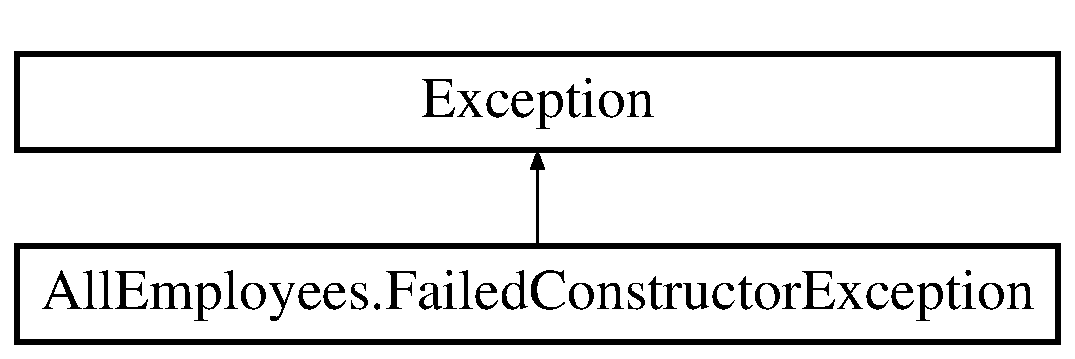
\includegraphics[height=2.000000cm]{class_all_employees_1_1_failed_constructor_exception}
\end{center}
\end{figure}
\subsection*{Public Member Functions}
\begin{DoxyCompactItemize}
\item 
\hyperlink{class_all_employees_1_1_failed_constructor_exception_a78d117eff5ea056d0076b601274f382d}{Failed\+Constructor\+Exception} ()
\begin{DoxyCompactList}\small\item\em default constructor. Create a \hyperlink{class_all_employees_1_1_failed_constructor_exception}{Failed\+Constructor\+Exception} with base Exception class \end{DoxyCompactList}\item 
\hyperlink{class_all_employees_1_1_failed_constructor_exception_a41c940dd9d247e852c71b49788754e9f}{Failed\+Constructor\+Exception} (string message)
\begin{DoxyCompactList}\small\item\em overloaded constructor. Create a \hyperlink{class_all_employees_1_1_failed_constructor_exception}{Failed\+Constructor\+Exception} with base Exception class and message \end{DoxyCompactList}\end{DoxyCompactItemize}


\subsection{Detailed Description}
{\bfseries Brief Description} The \hyperlink{class_all_employees_1_1_failed_constructor_exception}{Failed\+Constructor\+Exception} is a exception that will be thrown if the object the constructor creates is not a valid employee \hyperlink{class_all_employees_1_1_failed_constructor_exception}{Failed\+Constructor\+Exception} is a child of the Exception class 

\begin{DoxyAuthor}{Author}
{\itshape Brandon} 
\end{DoxyAuthor}


\subsection{Constructor \& Destructor Documentation}
\hypertarget{class_all_employees_1_1_failed_constructor_exception_a78d117eff5ea056d0076b601274f382d}{}\index{All\+Employees\+::\+Failed\+Constructor\+Exception@{All\+Employees\+::\+Failed\+Constructor\+Exception}!Failed\+Constructor\+Exception@{Failed\+Constructor\+Exception}}
\index{Failed\+Constructor\+Exception@{Failed\+Constructor\+Exception}!All\+Employees\+::\+Failed\+Constructor\+Exception@{All\+Employees\+::\+Failed\+Constructor\+Exception}}
\subsubsection[{Failed\+Constructor\+Exception}]{\setlength{\rightskip}{0pt plus 5cm}All\+Employees.\+Failed\+Constructor\+Exception.\+Failed\+Constructor\+Exception (
\begin{DoxyParamCaption}
{}
\end{DoxyParamCaption}
)}\label{class_all_employees_1_1_failed_constructor_exception_a78d117eff5ea056d0076b601274f382d}


default constructor. Create a \hyperlink{class_all_employees_1_1_failed_constructor_exception}{Failed\+Constructor\+Exception} with base Exception class 

{\bfseries Details}


\begin{DoxyParams}{Parameters}
{\em n/a} & \\
\hline
\end{DoxyParams}
\begin{DoxyReturn}{Returns}
n/a 
\end{DoxyReturn}
\hypertarget{class_all_employees_1_1_failed_constructor_exception_a41c940dd9d247e852c71b49788754e9f}{}\index{All\+Employees\+::\+Failed\+Constructor\+Exception@{All\+Employees\+::\+Failed\+Constructor\+Exception}!Failed\+Constructor\+Exception@{Failed\+Constructor\+Exception}}
\index{Failed\+Constructor\+Exception@{Failed\+Constructor\+Exception}!All\+Employees\+::\+Failed\+Constructor\+Exception@{All\+Employees\+::\+Failed\+Constructor\+Exception}}
\subsubsection[{Failed\+Constructor\+Exception}]{\setlength{\rightskip}{0pt plus 5cm}All\+Employees.\+Failed\+Constructor\+Exception.\+Failed\+Constructor\+Exception (
\begin{DoxyParamCaption}
\item[{string}]{message}
\end{DoxyParamCaption}
)}\label{class_all_employees_1_1_failed_constructor_exception_a41c940dd9d247e852c71b49788754e9f}


overloaded constructor. Create a \hyperlink{class_all_employees_1_1_failed_constructor_exception}{Failed\+Constructor\+Exception} with base Exception class and message 

{\bfseries Details}


\begin{DoxyParams}{Parameters}
{\em message} & {\bfseries string} -\/ the message to be attached to the exception\\
\hline
\end{DoxyParams}
\begin{DoxyReturn}{Returns}
n/a 
\end{DoxyReturn}


The documentation for this class was generated from the following file\+:\begin{DoxyCompactItemize}
\item 
C\+:/\+S\+E\+T\+Repo/trunk/\+E\+M\+S/trunk/\+All\+Employees/\+All\+Employees/Failed\+Constructor\+Exception.\+cs\end{DoxyCompactItemize}

\hypertarget{class_supporting_1_1_file_i_o}{}\section{Supporting.\+File\+I\+O Class Reference}
\label{class_supporting_1_1_file_i_o}\index{Supporting.\+File\+I\+O@{Supporting.\+File\+I\+O}}


{\bfseries Brief Description} This class allows files to be written to, read all the data from a file, open a file for reading, open a file for writing, closing a file and parsing data from a file. The file\+I\+O class is realted to employee and container class  


\subsection*{Public Member Functions}
\begin{DoxyCompactItemize}
\item 
List$<$ \hyperlink{class_all_employees_1_1_employee}{All\+Employees.\+Employee} $>$ \hyperlink{class_supporting_1_1_file_i_o_ab33154b7acbb27ecaee49cfe701691e7}{Read\+All\+Records} (String file\+Name)
\begin{DoxyCompactList}\small\item\em Give file name, return list of all valid records. \end{DoxyCompactList}\item 
void \hyperlink{class_supporting_1_1_file_i_o_a23293f70ec655e87ea568ffada174b9f}{Write\+Record} (\hyperlink{class_all_employees_1_1_employee}{All\+Employees.\+Employee} Employee, String file\+Name)
\begin{DoxyCompactList}\small\item\em Give employee write and file to write to. \end{DoxyCompactList}\end{DoxyCompactItemize}
\subsection*{Private Member Functions}
\begin{DoxyCompactItemize}
\item 
File\+Stream \hyperlink{class_supporting_1_1_file_i_o_ac9cebd77d6aca1292566d7e6eb4f8123}{Open\+File\+For\+Read} (String file\+Name)
\begin{DoxyCompactList}\small\item\em Give file name, return file for reading. \end{DoxyCompactList}\item 
File\+Stream \hyperlink{class_supporting_1_1_file_i_o_ab3be0f867327310b9d940d79e1147b69}{Open\+File\+For\+Write} (String file\+Name)
\begin{DoxyCompactList}\small\item\em Give file name, return file for writing. \end{DoxyCompactList}\item 
void \hyperlink{class_supporting_1_1_file_i_o_a689379fbd7441f18477d01dfde06444c}{Close\+File} (File\+Stream file)
\begin{DoxyCompactList}\small\item\em Closes the file. \end{DoxyCompactList}\item 
List$<$ \hyperlink{class_all_employees_1_1_employee}{All\+Employees.\+Employee} $>$ \hyperlink{class_supporting_1_1_file_i_o_ab4433298adf44f58cbd355eb5db0bf7f}{Pars\+Record} (String file\+Text)
\begin{DoxyCompactList}\small\item\em given string from file, pars all data into list, return list valid employees \end{DoxyCompactList}\end{DoxyCompactItemize}


\subsection{Detailed Description}
{\bfseries Brief Description} This class allows files to be written to, read all the data from a file, open a file for reading, open a file for writing, closing a file and parsing data from a file. The file\+I\+O class is realted to employee and container class 

\begin{DoxyAuthor}{Author}
{\itshape Nathan} 
\end{DoxyAuthor}


\subsection{Member Function Documentation}
\hypertarget{class_supporting_1_1_file_i_o_a689379fbd7441f18477d01dfde06444c}{}\index{Supporting\+::\+File\+I\+O@{Supporting\+::\+File\+I\+O}!Close\+File@{Close\+File}}
\index{Close\+File@{Close\+File}!Supporting\+::\+File\+I\+O@{Supporting\+::\+File\+I\+O}}
\subsubsection[{Close\+File}]{\setlength{\rightskip}{0pt plus 5cm}void Supporting.\+File\+I\+O.\+Close\+File (
\begin{DoxyParamCaption}
\item[{File\+Stream}]{file}
\end{DoxyParamCaption}
)\hspace{0.3cm}{\ttfamily [private]}}\label{class_supporting_1_1_file_i_o_a689379fbd7441f18477d01dfde06444c}


Closes the file. 

{\bfseries Details}


\begin{DoxyParams}{Parameters}
{\em file} & -\/ {\bfseries File\+Stream} -\/ The file to be closed\\
\hline
\end{DoxyParams}
\begin{DoxyReturn}{Returns}
n/a 
\end{DoxyReturn}
\hypertarget{class_supporting_1_1_file_i_o_ac9cebd77d6aca1292566d7e6eb4f8123}{}\index{Supporting\+::\+File\+I\+O@{Supporting\+::\+File\+I\+O}!Open\+File\+For\+Read@{Open\+File\+For\+Read}}
\index{Open\+File\+For\+Read@{Open\+File\+For\+Read}!Supporting\+::\+File\+I\+O@{Supporting\+::\+File\+I\+O}}
\subsubsection[{Open\+File\+For\+Read}]{\setlength{\rightskip}{0pt plus 5cm}File\+Stream Supporting.\+File\+I\+O.\+Open\+File\+For\+Read (
\begin{DoxyParamCaption}
\item[{String}]{file\+Name}
\end{DoxyParamCaption}
)\hspace{0.3cm}{\ttfamily [private]}}\label{class_supporting_1_1_file_i_o_ac9cebd77d6aca1292566d7e6eb4f8123}


Give file name, return file for reading. 

{\bfseries Details}


\begin{DoxyParams}{Parameters}
{\em file\+Name} & -\/ {\bfseries string} -\/ The file path and name of file storing the records\\
\hline
\end{DoxyParams}
\begin{DoxyReturn}{Returns}
read\+File -\/ {\bfseries File\+Stream} -\/ The opened file to be read 
\end{DoxyReturn}
\hypertarget{class_supporting_1_1_file_i_o_ab3be0f867327310b9d940d79e1147b69}{}\index{Supporting\+::\+File\+I\+O@{Supporting\+::\+File\+I\+O}!Open\+File\+For\+Write@{Open\+File\+For\+Write}}
\index{Open\+File\+For\+Write@{Open\+File\+For\+Write}!Supporting\+::\+File\+I\+O@{Supporting\+::\+File\+I\+O}}
\subsubsection[{Open\+File\+For\+Write}]{\setlength{\rightskip}{0pt plus 5cm}File\+Stream Supporting.\+File\+I\+O.\+Open\+File\+For\+Write (
\begin{DoxyParamCaption}
\item[{String}]{file\+Name}
\end{DoxyParamCaption}
)\hspace{0.3cm}{\ttfamily [private]}}\label{class_supporting_1_1_file_i_o_ab3be0f867327310b9d940d79e1147b69}


Give file name, return file for writing. 

{\bfseries Details}


\begin{DoxyParams}{Parameters}
{\em file\+Name} & -\/ {\bfseries string} -\/ The file path and name of file storing the records\\
\hline
\end{DoxyParams}
\begin{DoxyReturn}{Returns}
write\+File -\/ {\bfseries File\+Stream} -\/ The opened file to be written to 
\end{DoxyReturn}
\hypertarget{class_supporting_1_1_file_i_o_ab4433298adf44f58cbd355eb5db0bf7f}{}\index{Supporting\+::\+File\+I\+O@{Supporting\+::\+File\+I\+O}!Pars\+Record@{Pars\+Record}}
\index{Pars\+Record@{Pars\+Record}!Supporting\+::\+File\+I\+O@{Supporting\+::\+File\+I\+O}}
\subsubsection[{Pars\+Record}]{\setlength{\rightskip}{0pt plus 5cm}List$<${\bf All\+Employees.\+Employee}$>$ Supporting.\+File\+I\+O.\+Pars\+Record (
\begin{DoxyParamCaption}
\item[{String}]{file\+Text}
\end{DoxyParamCaption}
)\hspace{0.3cm}{\ttfamily [private]}}\label{class_supporting_1_1_file_i_o_ab4433298adf44f58cbd355eb5db0bf7f}


given string from file, pars all data into list, return list valid employees 

{\bfseries Details}


\begin{DoxyParams}{Parameters}
{\em file\+Text} & -\/ {\bfseries string} -\/ The string of data containing an employees records\\
\hline
\end{DoxyParams}
\begin{DoxyReturn}{Returns}
employee\+Rec -\/ {\bfseries List$<$\+All\+Employees.\+Employee$>$} -\/ The list of all the employee records in the strinng of data 
\end{DoxyReturn}
\hypertarget{class_supporting_1_1_file_i_o_ab33154b7acbb27ecaee49cfe701691e7}{}\index{Supporting\+::\+File\+I\+O@{Supporting\+::\+File\+I\+O}!Read\+All\+Records@{Read\+All\+Records}}
\index{Read\+All\+Records@{Read\+All\+Records}!Supporting\+::\+File\+I\+O@{Supporting\+::\+File\+I\+O}}
\subsubsection[{Read\+All\+Records}]{\setlength{\rightskip}{0pt plus 5cm}List$<${\bf All\+Employees.\+Employee}$>$ Supporting.\+File\+I\+O.\+Read\+All\+Records (
\begin{DoxyParamCaption}
\item[{String}]{file\+Name}
\end{DoxyParamCaption}
)}\label{class_supporting_1_1_file_i_o_ab33154b7acbb27ecaee49cfe701691e7}


Give file name, return list of all valid records. 

{\bfseries Details}


\begin{DoxyParams}{Parameters}
{\em file\+Name} & -\/ {\bfseries string} -\/ The file path and name of file storing the records\\
\hline
\end{DoxyParams}
\begin{DoxyReturn}{Returns}
employee\+Rec -\/ {\bfseries List$<$\+All\+Employees.\+Employee$>$} -\/ The list of all the employee records in the file 
\end{DoxyReturn}
\hypertarget{class_supporting_1_1_file_i_o_a23293f70ec655e87ea568ffada174b9f}{}\index{Supporting\+::\+File\+I\+O@{Supporting\+::\+File\+I\+O}!Write\+Record@{Write\+Record}}
\index{Write\+Record@{Write\+Record}!Supporting\+::\+File\+I\+O@{Supporting\+::\+File\+I\+O}}
\subsubsection[{Write\+Record}]{\setlength{\rightskip}{0pt plus 5cm}void Supporting.\+File\+I\+O.\+Write\+Record (
\begin{DoxyParamCaption}
\item[{{\bf All\+Employees.\+Employee}}]{Employee, }
\item[{String}]{file\+Name}
\end{DoxyParamCaption}
)}\label{class_supporting_1_1_file_i_o_a23293f70ec655e87ea568ffada174b9f}


Give employee write and file to write to. 

{\bfseries Details}


\begin{DoxyParams}{Parameters}
{\em Employee} & -\/ {\bfseries \hyperlink{class_all_employees_1_1_employee}{All\+Employees.\+Employee}} -\/ The employees records \\
\hline
{\em file\+Name} & -\/ {\bfseries String} -\/ The file path and name of file storing the records\\
\hline
\end{DoxyParams}
\begin{DoxyReturn}{Returns}
n/a 
\end{DoxyReturn}


The documentation for this class was generated from the following file\+:\begin{DoxyCompactItemize}
\item 
C\+:/\+S\+E\+T\+Repo/trunk/\+E\+M\+S/trunk/\+Supporting/\+Supporting/File\+I\+O.\+cs\end{DoxyCompactItemize}

\hypertarget{class_file_i_o_tests}{}\section{File\+I\+O\+Tests Class Reference}
\label{class_file_i_o_tests}\index{File\+I\+O\+Tests@{File\+I\+O\+Tests}}


{\bfseries  Brief Description} This class is used to test the Methods in the File\+I\+O class. The methods tested include Write\+Record, Read\+All\+Records, Pars\+Record. Read\+All\+Records inherantly uses Pars\+Record so they are tested at the same time  




\subsection{Detailed Description}
{\bfseries  Brief Description} This class is used to test the Methods in the File\+I\+O class. The methods tested include Write\+Record, Read\+All\+Records, Pars\+Record. Read\+All\+Records inherantly uses Pars\+Record so they are tested at the same time 

The documentation for this class was generated from the following file\+:\begin{DoxyCompactItemize}
\item 
C\+:/\+S\+E\+T\+Repo/trunk/\+E\+M\+S/trunk/\+Supporting/\+File\+I\+O.\+Tests/File\+I\+O\+Tests.\+cs\end{DoxyCompactItemize}

\hypertarget{class_file_i_o_tests_1_1_file_i_o_tests}{}\section{File\+I\+O\+Tests.\+File\+I\+O\+Tests Class Reference}
\label{class_file_i_o_tests_1_1_file_i_o_tests}\index{File\+I\+O\+Tests.\+File\+I\+O\+Tests@{File\+I\+O\+Tests.\+File\+I\+O\+Tests}}
\subsection*{Public Member Functions}
\begin{DoxyCompactItemize}
\item 
void \hyperlink{class_file_i_o_tests_1_1_file_i_o_tests_a5576e74011efb2c59ee879ff52d6adab}{write\+Good\+Data\+To\+Empty\+File\+C\+T} ()
\begin{DoxyCompactList}\small\item\em The unit test\textquotesingle{}s purpose is to test if the method Write\+Record will write a valid contract employee to a empty file. \end{DoxyCompactList}\item 
void \hyperlink{class_file_i_o_tests_1_1_file_i_o_tests_a26f35013ab03e8e1b781b73824fae84e}{write\+Good\+Data\+To\+Empty\+File\+F\+T} ()
\begin{DoxyCompactList}\small\item\em The unit test\textquotesingle{}s purpose is to test if the method Write\+Record will write a valid full time employee to a empty file. \end{DoxyCompactList}\item 
void \hyperlink{class_file_i_o_tests_1_1_file_i_o_tests_af4f229c45a4170ea087d7791d942f1bc}{write\+Good\+Data\+To\+Empty\+File\+P\+T} ()
\begin{DoxyCompactList}\small\item\em The unit test\textquotesingle{}s purpose is to test if the method Write\+Record will write a valid part time employee to a empty file. \end{DoxyCompactList}\item 
void \hyperlink{class_file_i_o_tests_1_1_file_i_o_tests_af51dab6545c7cc79a53c059a23b121f5}{write\+Good\+Data\+To\+Empty\+File\+S\+N} ()
\begin{DoxyCompactList}\small\item\em The unit test\textquotesingle{}s purpose is to test if the method Write\+Record will write a valid seasonal employee to a empty file. \end{DoxyCompactList}\item 
void \hyperlink{class_file_i_o_tests_1_1_file_i_o_tests_ad39e7e6da79929bc94d459fdbd4e67db}{write\+Good\+Data\+Existing\+File\+C\+T} ()
\begin{DoxyCompactList}\small\item\em The unit test\textquotesingle{}s purpose is to test if the method Write\+Record will write a valid contract employee to a existing file. \end{DoxyCompactList}\item 
void \hyperlink{class_file_i_o_tests_1_1_file_i_o_tests_ac8692223bba5d32d6671b8d20e57a5a1}{write\+Good\+Data\+Existing\+File\+F\+T} ()
\begin{DoxyCompactList}\small\item\em The unit test\textquotesingle{}s purpose is to test if the method Write\+Record will write a valid full time employee to a existing file. \end{DoxyCompactList}\item 
void \hyperlink{class_file_i_o_tests_1_1_file_i_o_tests_ac1b4e455917b40938344801e8463038a}{write\+Good\+Data\+Existing\+File\+P\+T} ()
\begin{DoxyCompactList}\small\item\em The unit test\textquotesingle{}s purpose is to test if the method Write\+Record will write a valid part time employee to a exisiting file. \end{DoxyCompactList}\item 
void \hyperlink{class_file_i_o_tests_1_1_file_i_o_tests_a03e8b6ab0681621f1dbb85fd66ace4bd}{write\+Good\+Data\+Existing\+File\+S\+N} ()
\begin{DoxyCompactList}\small\item\em The unit test\textquotesingle{}s purpose is to test if the method Write\+Record will write a valid seasonal employee to a exisiting file. \end{DoxyCompactList}\item 
void \hyperlink{class_file_i_o_tests_1_1_file_i_o_tests_acfe0df2ca6406249ebfe55e37dd6e162}{read\+Good\+Data} ()
\begin{DoxyCompactList}\small\item\em The unit test\textquotesingle{}s purpose is to test if the method Read\+All\+Records will read four valid employees, one for each type of employee and return those employees to a list. \end{DoxyCompactList}\item 
void \hyperlink{class_file_i_o_tests_1_1_file_i_o_tests_aa4b0c4cad279bedd3e72f95f6e2a8e37}{read\+Bad\+C\+T\+First\+Name\+Data} ()
\begin{DoxyCompactList}\small\item\em The unit test\textquotesingle{}s purpose is to test if the method Read\+All\+Records will read a contract employee with an invalid first name and not return that employee in a list. \end{DoxyCompactList}\item 
void \hyperlink{class_file_i_o_tests_1_1_file_i_o_tests_aa64a71c55fc17508c8551b9e409253aa}{read\+Bad\+F\+T\+First\+Name\+Data} ()
\begin{DoxyCompactList}\small\item\em The unit test\textquotesingle{}s purpose is to test if the method Read\+All\+Records will read a full time employees with an invalid first name and not return that employee in a list. \end{DoxyCompactList}\item 
void \hyperlink{class_file_i_o_tests_1_1_file_i_o_tests_a8c1903b58f09401fa2b43d9f6b4edc2a}{read\+Bad\+P\+T\+First\+Name\+Data} ()
\begin{DoxyCompactList}\small\item\em The unit test\textquotesingle{}s purpose is to test if the method Read\+All\+Records will read a part time employee with an invalid first name and not return that employee in a list. \end{DoxyCompactList}\item 
void \hyperlink{class_file_i_o_tests_1_1_file_i_o_tests_a36342a1b5ca8abbb5d2e7b437b73653f}{read\+Bad\+S\+N\+First\+Name\+Data} ()
\begin{DoxyCompactList}\small\item\em The unit test\textquotesingle{}s purpose is to test if the method Read\+All\+Records will read a seasonal employee with an invalid first name and not return that employee in a list. \end{DoxyCompactList}\item 
void \hyperlink{class_file_i_o_tests_1_1_file_i_o_tests_aabcbda743af2ce41d9e4be026d03a8d1}{read\+Bad\+C\+T\+Last\+Name\+Data} ()
\begin{DoxyCompactList}\small\item\em The unit test\textquotesingle{}s purpose is to test if the method Read\+All\+Records will read a contract employee with an invalid last name and not return that employee in a list. \end{DoxyCompactList}\item 
void \hyperlink{class_file_i_o_tests_1_1_file_i_o_tests_a65a82c433721ab579d47dffefbf27876}{read\+Bad\+F\+T\+Last\+Name\+Data} ()
\begin{DoxyCompactList}\small\item\em The unit test\textquotesingle{}s purpose is to test if the method Read\+All\+Records will read a full time employee with an invalid last name and not return that employee in a list. \end{DoxyCompactList}\item 
void \hyperlink{class_file_i_o_tests_1_1_file_i_o_tests_a73dbb713735d66b7744de925f2f8e529}{read\+Bad\+P\+T\+Last\+Name\+Data} ()
\begin{DoxyCompactList}\small\item\em The unit test\textquotesingle{}s purpose is to test if the method Read\+All\+Records will read a part time employee with an invalid last name and not return that employee in a list. \end{DoxyCompactList}\item 
void \hyperlink{class_file_i_o_tests_1_1_file_i_o_tests_a2e633e57ec62bb740be9d40341c8f15a}{read\+Bad\+S\+N\+Last\+Name\+Data} ()
\begin{DoxyCompactList}\small\item\em The unit test\textquotesingle{}s purpose is to test if the method Read\+All\+Records will read a seasonal employee with an invalid last name and not return that employee in a list. \end{DoxyCompactList}\item 
void \hyperlink{class_file_i_o_tests_1_1_file_i_o_tests_a59c16b6763506888dd7d7d11dc3e9fca}{read\+Bad\+C\+T\+Social\+Insurance\+Number\+Data} ()
\begin{DoxyCompactList}\small\item\em The unit test\textquotesingle{}s purpose is to test if the method Read\+All\+Records will read a contract employee with an invalid social insurance number and not return that employee in a list. \end{DoxyCompactList}\item 
void \hyperlink{class_file_i_o_tests_1_1_file_i_o_tests_a9a69d9d30331bea2e36dcd41bc6393b7}{read\+Bad\+F\+T\+Social\+Insurance\+Number\+Data} ()
\begin{DoxyCompactList}\small\item\em The unit test\textquotesingle{}s purpose is to test if the method Read\+All\+Records will read a full time employee with an invalid social insurance number and not return that employee in a list. \end{DoxyCompactList}\item 
void \hyperlink{class_file_i_o_tests_1_1_file_i_o_tests_a1742ca38a92a76dea23805e7927573d5}{read\+Bad\+P\+T\+Social\+Insurance\+Number\+Data} ()
\begin{DoxyCompactList}\small\item\em The unit test\textquotesingle{}s purpose is to test if the method Read\+All\+Records will read a part time employee with an invalid social insurance number and not return that employee in a list. \end{DoxyCompactList}\item 
void \hyperlink{class_file_i_o_tests_1_1_file_i_o_tests_a2b1261c39b325a04da207fe35095b58a}{read\+Bad\+S\+N\+Social\+Insurance\+Number\+Data} ()
\begin{DoxyCompactList}\small\item\em The unit test\textquotesingle{}s purpose is to test if the method Read\+All\+Records will read a seasonal employee with an invalid social insurance number and not return that employee in a list. \end{DoxyCompactList}\item 
void \hyperlink{class_file_i_o_tests_1_1_file_i_o_tests_a0655cfd9e705deaa02599ba1533270ef}{read\+Bad\+C\+T\+Date\+Of\+Birth\+Data} ()
\begin{DoxyCompactList}\small\item\em The unit test\textquotesingle{}s purpose is to test if the method Read\+All\+Records will read a contract employee with an invalid date of birth and not return that employee in a list. \end{DoxyCompactList}\item 
void \hyperlink{class_file_i_o_tests_1_1_file_i_o_tests_ac547d3676534cc2207e3ff806504f745}{read\+Bad\+F\+T\+Date\+Of\+Birth\+Data} ()
\begin{DoxyCompactList}\small\item\em The unit test\textquotesingle{}s purpose is to test if the method Read\+All\+Records will read a full time employee with an invalid date of birth and not return that employee in a list. \end{DoxyCompactList}\item 
void \hyperlink{class_file_i_o_tests_1_1_file_i_o_tests_af6ec136300bc783b54a4253dbab0d73c}{read\+Bad\+P\+T\+Date\+Of\+Birth\+Data} ()
\begin{DoxyCompactList}\small\item\em The unit test\textquotesingle{}s purpose is to test if the method Read\+All\+Records will read a part time employee with an invalid date of birth and not return that employee in a list. \end{DoxyCompactList}\item 
void \hyperlink{class_file_i_o_tests_1_1_file_i_o_tests_aaef88f336ac31b90daecef832d40c560}{read\+Bad\+S\+N\+Date\+Of\+Birth\+Data} ()
\begin{DoxyCompactList}\small\item\em The unit test\textquotesingle{}s purpose is to test if the method Read\+All\+Records will read a seasonal employee with an invalid date of birth and not return that employee in a list. \end{DoxyCompactList}\item 
void \hyperlink{class_file_i_o_tests_1_1_file_i_o_tests_a6867a128f3c6430639c6152237d723de}{read\+Bad\+C\+T\+Contract\+Start\+Date\+Data} ()
\begin{DoxyCompactList}\small\item\em The unit test\textquotesingle{}s purpose is to test if the method Read\+All\+Records will read a contract employee with an invalid start date and not return that employee in a list. \end{DoxyCompactList}\item 
void \hyperlink{class_file_i_o_tests_1_1_file_i_o_tests_a8934e2ab8df733979ff977276a9d89ab}{read\+Bad\+F\+T\+Contract\+Start\+Date\+Data} ()
\begin{DoxyCompactList}\small\item\em The unit test\textquotesingle{}s purpose is to test if the method Read\+All\+Records will read a full time employee with an invalid start date and not return that employee in a list. \end{DoxyCompactList}\item 
void \hyperlink{class_file_i_o_tests_1_1_file_i_o_tests_ae61f702c7175f65f4e831873b9baaf2c}{read\+Bad\+P\+T\+Contract\+Start\+Date\+Data} ()
\begin{DoxyCompactList}\small\item\em The unit test\textquotesingle{}s purpose is to test if the method Read\+All\+Records will read a part time employee with an invalid start date and not return that employee in a list. \end{DoxyCompactList}\item 
void \hyperlink{class_file_i_o_tests_1_1_file_i_o_tests_a27a923a5933172ad163f750dcb3c0d97}{read\+Bad\+S\+N\+Season\+Data} ()
\begin{DoxyCompactList}\small\item\em The unit test\textquotesingle{}s purpose is to test if the method Read\+All\+Records will read a seasonal employee with an invalid season and not return that employee in a list. \end{DoxyCompactList}\item 
void \hyperlink{class_file_i_o_tests_1_1_file_i_o_tests_a6868dfec978501a6b229448ad52cd739}{read\+Bad\+C\+T\+Contract\+Stop\+Date\+Data} ()
\begin{DoxyCompactList}\small\item\em The unit test\textquotesingle{}s purpose is to test if the method Read\+All\+Records will read a contract employee with an invalid stop date and not return that employee in a list. \end{DoxyCompactList}\item 
void \hyperlink{class_file_i_o_tests_1_1_file_i_o_tests_ae165da96652fbc78738b73b24039c98c}{read\+Bad\+F\+T\+Contract\+Stop\+Date\+Data} ()
\begin{DoxyCompactList}\small\item\em The unit test\textquotesingle{}s purpose is to test if the method Read\+All\+Records will read a full time employee with an invalid stop date and not return that employee in a list. \end{DoxyCompactList}\item 
void \hyperlink{class_file_i_o_tests_1_1_file_i_o_tests_a435a53b04da8e49cbfe4cd61eacfc43a}{read\+Bad\+P\+T\+Contract\+Stop\+Date\+Data} ()
\begin{DoxyCompactList}\small\item\em The unit test\textquotesingle{}s purpose is to test if the method Read\+All\+Records will read a part time employee with an invalid stop date and not return that employee in a list. \end{DoxyCompactList}\item 
void \hyperlink{class_file_i_o_tests_1_1_file_i_o_tests_afd9078725a0f46f01d090dc668e94ab0}{read\+Bad\+S\+N\+Piece\+Pay\+Data} ()
\begin{DoxyCompactList}\small\item\em The unit test\textquotesingle{}s purpose is to test if the method Read\+All\+Records will read a seasonal employee with an invalid piece pay and not return that employee in a list. \end{DoxyCompactList}\item 
void \hyperlink{class_file_i_o_tests_1_1_file_i_o_tests_adc390277bbcc6105ef453ffb70baea2e}{read\+Bad\+C\+Tfixed\+Contract\+Amount\+Data} ()
\begin{DoxyCompactList}\small\item\em The unit test\textquotesingle{}s purpose is to test if the method Read\+All\+Records will read a contract employee with an invalid contract amount and not return that employee in a list. \end{DoxyCompactList}\item 
void \hyperlink{class_file_i_o_tests_1_1_file_i_o_tests_a88d92a5da0f6478319611217bdcba396}{read\+Bad\+F\+Tfixed\+Contract\+Amount\+Data} ()
\begin{DoxyCompactList}\small\item\em The unit test\textquotesingle{}s purpose is to test if the method Read\+All\+Records will read a full time employee with an invalid contract amount and not return that employee in a list. \end{DoxyCompactList}\item 
void \hyperlink{class_file_i_o_tests_1_1_file_i_o_tests_a6ec660d41c990bb03db721493c55e6f7}{read\+Bad\+P\+Tfixed\+Contract\+Amount\+Data} ()
\begin{DoxyCompactList}\small\item\em The unit test\textquotesingle{}s purpose is to test if the method Read\+All\+Records will read a part time employee with an invalid contract amount and not return that employee in a list. \end{DoxyCompactList}\item 
void \hyperlink{class_file_i_o_tests_1_1_file_i_o_tests_a4b5f10c5a9a384b3e37d2de6fc34ea4c}{read\+Missing\+C\+T\+First\+Name\+Data} ()
\begin{DoxyCompactList}\small\item\em The unit test\textquotesingle{}s purpose is to test if the method Read\+All\+Records will read a contract employee with an missing first name and not return that employee in a list. \end{DoxyCompactList}\item 
void \hyperlink{class_file_i_o_tests_1_1_file_i_o_tests_a3b8f804ae1d432b8b9565c59d332a3d5}{read\+Missing\+F\+T\+First\+Name\+Data} ()
\begin{DoxyCompactList}\small\item\em The unit test\textquotesingle{}s purpose is to test if the method Read\+All\+Records will read a full time employee with an missing first name and not return that employee in a list. \end{DoxyCompactList}\item 
void \hyperlink{class_file_i_o_tests_1_1_file_i_o_tests_a18f69b088f8042a3e43cd43c7f4ab658}{read\+Missing\+P\+T\+First\+Name\+Data} ()
\begin{DoxyCompactList}\small\item\em The unit test\textquotesingle{}s purpose is to test if the method Read\+All\+Records will read a part time employee with an missing first name and not return that employee in a list. \end{DoxyCompactList}\item 
void \hyperlink{class_file_i_o_tests_1_1_file_i_o_tests_ae0b0cedc850efac31319b8f236d7871c}{read\+Missing\+S\+N\+First\+Name\+Data} ()
\begin{DoxyCompactList}\small\item\em The unit test\textquotesingle{}s purpose is to test if the method Read\+All\+Records will read a seasonal employee with an missing first name and not return that employee in a list. \end{DoxyCompactList}\item 
void \hyperlink{class_file_i_o_tests_1_1_file_i_o_tests_a55d29fa7f328d5f09012e21cf1e4e8fa}{read\+Missing\+C\+T\+Last\+Name\+Data} ()
\begin{DoxyCompactList}\small\item\em The unit test\textquotesingle{}s purpose is to test if the method Read\+All\+Records will read a contract employee with an missing last name and not return that employee in a list. \end{DoxyCompactList}\item 
void \hyperlink{class_file_i_o_tests_1_1_file_i_o_tests_a6dfd45892de70caf28049718709666d9}{read\+Missing\+F\+T\+Last\+Name\+Data} ()
\begin{DoxyCompactList}\small\item\em The unit test\textquotesingle{}s purpose is to test if the method Read\+All\+Records will read a full time employee with an missing last name and not return that employee in a list. \end{DoxyCompactList}\item 
void \hyperlink{class_file_i_o_tests_1_1_file_i_o_tests_aa71f71dbc3fb607eb95d7f6791476f18}{read\+Missing\+P\+T\+Last\+Name\+Data} ()
\begin{DoxyCompactList}\small\item\em The unit test\textquotesingle{}s purpose is to test if the method Read\+All\+Records will read a part time employee with an missing last name and not return that employee in a list. \end{DoxyCompactList}\item 
void \hyperlink{class_file_i_o_tests_1_1_file_i_o_tests_a558369745ee3a55e37bd0838a798e4ee}{read\+Missing\+S\+N\+Last\+Name\+Data} ()
\begin{DoxyCompactList}\small\item\em The unit test\textquotesingle{}s purpose is to test if the method Read\+All\+Records will read a seasonal employee with an missing last name and not return that employee in a list. \end{DoxyCompactList}\item 
void \hyperlink{class_file_i_o_tests_1_1_file_i_o_tests_a78376b361c09ca91f24c4baf66402ce4}{read\+Missing\+C\+T\+Social\+Insurance\+Number\+Data} ()
\begin{DoxyCompactList}\small\item\em The unit test\textquotesingle{}s purpose is to test if the method Read\+All\+Records will read a contract employee with an missing social insurance number and not return that employee in a list. \end{DoxyCompactList}\item 
void \hyperlink{class_file_i_o_tests_1_1_file_i_o_tests_af0277eefc9fcd4eca4c19ad04903fd59}{read\+Missing\+F\+T\+Social\+Insurance\+Number\+Data} ()
\begin{DoxyCompactList}\small\item\em The unit test\textquotesingle{}s purpose is to test if the method Read\+All\+Records will read a full time employee with an missing social insurance number and not return that employee in a list. \end{DoxyCompactList}\item 
void \hyperlink{class_file_i_o_tests_1_1_file_i_o_tests_a643039fe9be4f5293ecf7a3fac07a656}{read\+Missing\+P\+T\+Social\+Insurance\+Number\+Data} ()
\begin{DoxyCompactList}\small\item\em The unit test\textquotesingle{}s purpose is to test if the method Read\+All\+Records will read a part time employee with an missing social insurance number and not return that employee in a list. \end{DoxyCompactList}\item 
void \hyperlink{class_file_i_o_tests_1_1_file_i_o_tests_ae3be09f9751098f2c1387c0712890505}{read\+Missing\+S\+N\+Social\+Insurance\+Number\+Data} ()
\begin{DoxyCompactList}\small\item\em The unit test\textquotesingle{}s purpose is to test if the method Read\+All\+Records will read a seasonal employee with an missing social insurance number and not return that employee in a list. \end{DoxyCompactList}\item 
void \hyperlink{class_file_i_o_tests_1_1_file_i_o_tests_a76329c7f9c306810c578715d5da4449a}{read\+Missing\+C\+T\+Date\+Of\+Birth\+Data} ()
\begin{DoxyCompactList}\small\item\em The unit test\textquotesingle{}s purpose is to test if the method Read\+All\+Records will read a contract employee with a missing date of birth and not return that employee in a list. \end{DoxyCompactList}\item 
void \hyperlink{class_file_i_o_tests_1_1_file_i_o_tests_a236bb0dfcf65b8e80eac0a430d3cbb4e}{read\+Missing\+F\+T\+Date\+Of\+Birth\+Data} ()
\begin{DoxyCompactList}\small\item\em The unit test\textquotesingle{}s purpose is to test if the method Read\+All\+Records will read a full time employee with a missing date of birth and not return that employee in a list. \end{DoxyCompactList}\item 
void \hyperlink{class_file_i_o_tests_1_1_file_i_o_tests_ab139efe1757f96627b927bee9e04124d}{read\+Missing\+P\+T\+Date\+Of\+Birth\+Data} ()
\begin{DoxyCompactList}\small\item\em The unit test\textquotesingle{}s purpose is to test if the method Read\+All\+Records will read a part time employee with a missing date of birth and not return that employee in a list. \end{DoxyCompactList}\item 
void \hyperlink{class_file_i_o_tests_1_1_file_i_o_tests_a4303821c3a0580cb900ccc11907db56c}{read\+Missing\+S\+N\+Date\+Of\+Birth\+Data} ()
\begin{DoxyCompactList}\small\item\em The unit test\textquotesingle{}s purpose is to test if the method Read\+All\+Records will read a seasonal employee with a missing date of birth and not return that employee in a list. \end{DoxyCompactList}\item 
void \hyperlink{class_file_i_o_tests_1_1_file_i_o_tests_aee32f8a08dac9bcaff47cbab3a75ab37}{read\+Missing\+C\+T\+Contract\+Start\+Date\+Data} ()
\begin{DoxyCompactList}\small\item\em The unit test\textquotesingle{}s purpose is to test if the method Read\+All\+Records will read a contract employee with a missing start date and not return that employee in a list. \end{DoxyCompactList}\item 
void \hyperlink{class_file_i_o_tests_1_1_file_i_o_tests_ad678ce357b215214cde943b45b11dd43}{read\+Missing\+F\+T\+Date\+Of\+Hire\+Data} ()
\begin{DoxyCompactList}\small\item\em The unit test\textquotesingle{}s purpose is to test if the method Read\+All\+Records will read a full time employee with a missing start date and not return that employee in a list. \end{DoxyCompactList}\item 
void \hyperlink{class_file_i_o_tests_1_1_file_i_o_tests_ae6e7830712461fd1d303c09821c60527}{read\+Missing\+P\+T\+Date\+Of\+Hire\+Data} ()
\begin{DoxyCompactList}\small\item\em The unit test\textquotesingle{}s purpose is to test if the method Read\+All\+Records will read a part time employee with a missing start date and not return that employee in a list. \end{DoxyCompactList}\item 
void \hyperlink{class_file_i_o_tests_1_1_file_i_o_tests_a90be7ea571075a90ff102032830cd797}{read\+Missing\+S\+N\+Season\+Data} ()
\begin{DoxyCompactList}\small\item\em The unit test\textquotesingle{}s purpose is to test if the method Read\+All\+Records will read a seasonal employee with a missing season and not return that employee in a list. \end{DoxyCompactList}\item 
void \hyperlink{class_file_i_o_tests_1_1_file_i_o_tests_a0e304d2802533ca35e434bcf47e6defc}{read\+Missing\+C\+T\+Contract\+Stop\+Date\+Data} ()
\begin{DoxyCompactList}\small\item\em The unit test\textquotesingle{}s purpose is to test if the method Read\+All\+Records will read a contract employee with a missing stop date and not return that employee in a list. \end{DoxyCompactList}\item 
void \hyperlink{class_file_i_o_tests_1_1_file_i_o_tests_af43bf69b8856dd027852251783264787}{read\+Missing\+F\+T\+Date\+Of\+Termination\+Data} ()
\begin{DoxyCompactList}\small\item\em The unit test\textquotesingle{}s purpose is to test if the method Read\+All\+Records will read a full time employee with a missing stop date and not return that employee in a list. \end{DoxyCompactList}\item 
void \hyperlink{class_file_i_o_tests_1_1_file_i_o_tests_a5a6dcd3089b10fa0d79f7af555157abd}{read\+Missing\+P\+T\+Date\+Of\+Termination\+Data} ()
\begin{DoxyCompactList}\small\item\em The unit test\textquotesingle{}s purpose is to test if the method Read\+All\+Records will read a part time employee with a missing stop date and not return that employee in a list. \end{DoxyCompactList}\item 
void \hyperlink{class_file_i_o_tests_1_1_file_i_o_tests_ab3a9ef6366aef8c51026210a0ae0d8a0}{read\+Missing\+S\+N\+Piece\+Pay\+Data} ()
\begin{DoxyCompactList}\small\item\em The unit test\textquotesingle{}s purpose is to test if the method Read\+All\+Records will read a seasonal employee with a missing piece pay and not return that employee in a list. \end{DoxyCompactList}\item 
void \hyperlink{class_file_i_o_tests_1_1_file_i_o_tests_a849aa3c00169f82086afff072939fd9e}{read\+Missing\+C\+T\+Fixed\+Contract\+Amount\+Data} ()
\begin{DoxyCompactList}\small\item\em The unit test\textquotesingle{}s purpose is to test if the method Read\+All\+Records will read a contract employee with a missing contract amount and not return that employee in a list. \end{DoxyCompactList}\item 
void \hyperlink{class_file_i_o_tests_1_1_file_i_o_tests_a2b3560b4645c79de49974863cc5c7a52}{read\+Missing\+F\+T\+Salary\+Data} ()
\begin{DoxyCompactList}\small\item\em The unit test\textquotesingle{}s purpose is to test if the method Read\+All\+Records will read a full time employee with a missing salary and not return that employee in a list. \end{DoxyCompactList}\item 
void \hyperlink{class_file_i_o_tests_1_1_file_i_o_tests_a4d7449a49e50d385fdeb0ee8d346129a}{read\+Missing\+P\+T\+Hourly\+Rate\+Data} ()
\begin{DoxyCompactList}\small\item\em The unit test\textquotesingle{}s purpose is to test if the method Read\+All\+Records will read a part time employee with a missing hourly rate and not return that employee in a list. \end{DoxyCompactList}\item 
void \hyperlink{class_file_i_o_tests_1_1_file_i_o_tests_a1484a98ad13a6bcc1f428305a44c0329}{read\+Blank\+C\+T\+First\+Name\+Data} ()
\begin{DoxyCompactList}\small\item\em The unit test\textquotesingle{}s purpose is to test if the method Read\+All\+Records will read a contract employee with a blank first name and not return that employee in a list. \end{DoxyCompactList}\item 
void \hyperlink{class_file_i_o_tests_1_1_file_i_o_tests_a58310a35716d42d44af98881596d5fc7}{read\+Blank\+F\+T\+First\+Name\+Data} ()
\begin{DoxyCompactList}\small\item\em The unit test\textquotesingle{}s purpose is to test if the method Read\+All\+Records will read a full time employee with a blank first name and not return that employee in a list. \end{DoxyCompactList}\item 
void \hyperlink{class_file_i_o_tests_1_1_file_i_o_tests_a81583e556d22a53af94598f798550c06}{read\+Blank\+P\+T\+First\+Name\+Data} ()
\begin{DoxyCompactList}\small\item\em The unit test\textquotesingle{}s purpose is to test if the method Read\+All\+Records will read a part time employee with a blank first name and not return that employee in a list. \end{DoxyCompactList}\item 
void \hyperlink{class_file_i_o_tests_1_1_file_i_o_tests_ab5c4962dd7d6076fbb38d4642cee3dd2}{read\+Blank\+S\+N\+First\+Name\+Data} ()
\begin{DoxyCompactList}\small\item\em The unit test\textquotesingle{}s purpose is to test if the method Read\+All\+Records will read a seasonal employee with a blank first name and not return that employee in a list. \end{DoxyCompactList}\item 
void \hyperlink{class_file_i_o_tests_1_1_file_i_o_tests_aa1b1249b1659362a53ae771948797f61}{read\+Blank\+C\+T\+Last\+Name\+Data} ()
\begin{DoxyCompactList}\small\item\em The unit test\textquotesingle{}s purpose is to test if the method Read\+All\+Records will read a contract employee with a blank last name and not return that employee in a list. \end{DoxyCompactList}\item 
void \hyperlink{class_file_i_o_tests_1_1_file_i_o_tests_a63bac6e2d509044cfcbb504cf630910c}{read\+Blank\+F\+T\+Last\+Name\+Data} ()
\begin{DoxyCompactList}\small\item\em The unit test\textquotesingle{}s purpose is to test if the method Read\+All\+Records will read a full time employee with a blank last name and not return that employee in a list. \end{DoxyCompactList}\item 
void \hyperlink{class_file_i_o_tests_1_1_file_i_o_tests_a4633a95ed1e16bac8d2a527db223cee9}{read\+Blank\+P\+T\+Last\+Name\+Data} ()
\begin{DoxyCompactList}\small\item\em The unit test\textquotesingle{}s purpose is to test if the method Read\+All\+Records will read a part time employee with a blank last name and not return that employee in a list. \end{DoxyCompactList}\item 
void \hyperlink{class_file_i_o_tests_1_1_file_i_o_tests_a9479915b9a0b60beb1048ae3f152e33e}{read\+Blank\+S\+N\+Last\+Name\+Data} ()
\begin{DoxyCompactList}\small\item\em The unit test\textquotesingle{}s purpose is to test if the method Read\+All\+Records will read a seasonal employee with a blank last name and not return that employee in a list. \end{DoxyCompactList}\item 
void \hyperlink{class_file_i_o_tests_1_1_file_i_o_tests_a78d8b209df47110978848dc89257466d}{read\+Blank\+C\+T\+Social\+Insurance\+Number\+Data} ()
\begin{DoxyCompactList}\small\item\em The unit test\textquotesingle{}s purpose is to test if the method Read\+All\+Records will read a contract employee with a blank social insurance number and not return that employee in a list. \end{DoxyCompactList}\item 
void \hyperlink{class_file_i_o_tests_1_1_file_i_o_tests_a92f0c3877551434af09c16d14906228d}{read\+Blank\+F\+T\+Social\+Insurance\+Number\+Data} ()
\begin{DoxyCompactList}\small\item\em The unit test\textquotesingle{}s purpose is to test if the method Read\+All\+Records will read a full time employee with a blank social insurance number and not return that employee in a list. \end{DoxyCompactList}\item 
void \hyperlink{class_file_i_o_tests_1_1_file_i_o_tests_a48c165b62517080564d9cfd03496ab3a}{read\+Blank\+P\+T\+Social\+Insurance\+Number\+Data} ()
\begin{DoxyCompactList}\small\item\em The unit test\textquotesingle{}s purpose is to test if the method Read\+All\+Records will read a part time employee with a blank social insurance number and not return that employee in a list. \end{DoxyCompactList}\item 
void \hyperlink{class_file_i_o_tests_1_1_file_i_o_tests_acffed6026d192e58a743b84d019759c6}{read\+Blank\+S\+N\+Social\+Insurance\+Number\+Data} ()
\begin{DoxyCompactList}\small\item\em The unit test\textquotesingle{}s purpose is to test if the method Read\+All\+Records will read a seasonal employee with a blank social insurance number and not return that employee in a list. \end{DoxyCompactList}\item 
void \hyperlink{class_file_i_o_tests_1_1_file_i_o_tests_a15e9a988c3c2d76c266f4e6703f1a3e9}{read\+Blank\+C\+T\+Date\+Of\+Birth\+Data} ()
\begin{DoxyCompactList}\small\item\em The unit test\textquotesingle{}s purpose is to test if the method Read\+All\+Records will read a contract employee with a blank date of birth and not return that employee in a list. \end{DoxyCompactList}\item 
void \hyperlink{class_file_i_o_tests_1_1_file_i_o_tests_a9ae8eaeafcd739d8d91b20ada054b788}{read\+Blank\+F\+T\+Date\+Of\+Birth\+Data} ()
\begin{DoxyCompactList}\small\item\em The unit test\textquotesingle{}s purpose is to test if the method Read\+All\+Records will read a full time employee with a blank date of birth and not return that employee in a list. \end{DoxyCompactList}\item 
void \hyperlink{class_file_i_o_tests_1_1_file_i_o_tests_ad38321c2af440d038f198a952d8a7a5f}{read\+Blank\+P\+T\+Date\+Of\+Birth\+Data} ()
\begin{DoxyCompactList}\small\item\em The unit test\textquotesingle{}s purpose is to test if the method Read\+All\+Records will read a part time employee with a blank date of birth and not return that employee in a list. \end{DoxyCompactList}\item 
void \hyperlink{class_file_i_o_tests_1_1_file_i_o_tests_a91052ef2ab58e1f31c80e916e7aa5a78}{read\+Blank\+S\+N\+Date\+Of\+Birth\+Data} ()
\begin{DoxyCompactList}\small\item\em The unit test\textquotesingle{}s purpose is to test if the method Read\+All\+Records will read a seasonal employee with a blank date of birth and not return that employee in a list. \end{DoxyCompactList}\item 
void \hyperlink{class_file_i_o_tests_1_1_file_i_o_tests_a9362c9597624455d26cb42bb34a4f342}{read\+Blank\+C\+T\+Contract\+Start\+Date\+Data} ()
\begin{DoxyCompactList}\small\item\em The unit test\textquotesingle{}s purpose is to test if the method Read\+All\+Records will read a contract employee with a blank start date and not return that employee in a list. \end{DoxyCompactList}\item 
void \hyperlink{class_file_i_o_tests_1_1_file_i_o_tests_a000ec15aab13637cd8dc13b77ec1ef39}{read\+Blank\+F\+T\+Date\+Of\+Hire\+Data} ()
\begin{DoxyCompactList}\small\item\em The unit test\textquotesingle{}s purpose is to test if the method Read\+All\+Records will read a full time employee with a blank start date and not return that employee in a list. \end{DoxyCompactList}\item 
void \hyperlink{class_file_i_o_tests_1_1_file_i_o_tests_aefaac22298eec1af951af4ca2a42ede4}{read\+Blank\+P\+T\+Date\+Of\+Hire\+Data} ()
\begin{DoxyCompactList}\small\item\em The unit test\textquotesingle{}s purpose is to test if the method Read\+All\+Records will read a part time employee with a blank start date and not return that employee in a list. \end{DoxyCompactList}\item 
void \hyperlink{class_file_i_o_tests_1_1_file_i_o_tests_aca2cb3e7d051bad35675d663272af2ef}{read\+Blank\+S\+N\+Season\+Data} ()
\begin{DoxyCompactList}\small\item\em The unit test\textquotesingle{}s purpose is to test if the method Read\+All\+Records will read a seasonal employee with a blank season and not return that employee in a list. \end{DoxyCompactList}\item 
void \hyperlink{class_file_i_o_tests_1_1_file_i_o_tests_a629ae85c2e1179291498d84736051cc3}{read\+Blank\+C\+T\+Contract\+Stop\+Date\+Data} ()
\begin{DoxyCompactList}\small\item\em The unit test\textquotesingle{}s purpose is to test if the method Read\+All\+Records will read a contract employee with a blank stop date and return that employee in a list. \end{DoxyCompactList}\item 
void \hyperlink{class_file_i_o_tests_1_1_file_i_o_tests_a3c37b99e11e5fa0d3d44197c74c7dd2d}{read\+Blank\+F\+T\+Date\+Of\+Termination\+Data} ()
\begin{DoxyCompactList}\small\item\em The unit test\textquotesingle{}s purpose is to test if the method Read\+All\+Records will read a full time employee with a blank stop date and return that employee in a list. \end{DoxyCompactList}\item 
void \hyperlink{class_file_i_o_tests_1_1_file_i_o_tests_a196aabfeea5baa15b483e8ce4a658d18}{read\+Blank\+P\+T\+Date\+Of\+Termination\+Data} ()
\begin{DoxyCompactList}\small\item\em The unit test\textquotesingle{}s purpose is to test if the method Read\+All\+Records will read a part time employee with a blank stop date and return that employee in a list. \end{DoxyCompactList}\item 
void \hyperlink{class_file_i_o_tests_1_1_file_i_o_tests_a2662a873c3a9f56d949c0d1ad1ad2efc}{read\+Blank\+S\+N\+Piece\+Pay\+Data} ()
\begin{DoxyCompactList}\small\item\em The unit test\textquotesingle{}s purpose is to test if the method Read\+All\+Records will read a seasonal employee with a blank peice pay and not return that employee in a list. \end{DoxyCompactList}\item 
void \hyperlink{class_file_i_o_tests_1_1_file_i_o_tests_a1e89fba1e790dd6d8ecc86da746635a7}{read\+Blank\+C\+T\+Fixed\+Contract\+Amount\+Data} ()
\begin{DoxyCompactList}\small\item\em The unit test\textquotesingle{}s purpose is to test if the method Read\+All\+Records will read a contract employee with a blank contract and not return that employee in a list. \end{DoxyCompactList}\item 
void \hyperlink{class_file_i_o_tests_1_1_file_i_o_tests_a46a28774767e6ad2578f36c793206451}{read\+Blank\+F\+T\+Salary\+Data} ()
\begin{DoxyCompactList}\small\item\em The unit test\textquotesingle{}s purpose is to test if the method Read\+All\+Records will read a full time employee with a blank salary and not return that employee in a list. \end{DoxyCompactList}\item 
void \hyperlink{class_file_i_o_tests_1_1_file_i_o_tests_ac0aecca931032054e68587984cd6562a}{read\+Blank\+P\+T\+Hourly\+Rate\+Data} ()
\begin{DoxyCompactList}\small\item\em The unit test\textquotesingle{}s purpose is to test if the method Read\+All\+Records will read a part time employee with a blank hour rate and not return that employee in a list. \end{DoxyCompactList}\end{DoxyCompactItemize}


\subsection{Member Function Documentation}
\hypertarget{class_file_i_o_tests_1_1_file_i_o_tests_a6867a128f3c6430639c6152237d723de}{}\index{File\+I\+O\+Tests\+::\+File\+I\+O\+Tests@{File\+I\+O\+Tests\+::\+File\+I\+O\+Tests}!read\+Bad\+C\+T\+Contract\+Start\+Date\+Data@{read\+Bad\+C\+T\+Contract\+Start\+Date\+Data}}
\index{read\+Bad\+C\+T\+Contract\+Start\+Date\+Data@{read\+Bad\+C\+T\+Contract\+Start\+Date\+Data}!File\+I\+O\+Tests\+::\+File\+I\+O\+Tests@{File\+I\+O\+Tests\+::\+File\+I\+O\+Tests}}
\subsubsection[{read\+Bad\+C\+T\+Contract\+Start\+Date\+Data}]{\setlength{\rightskip}{0pt plus 5cm}void File\+I\+O\+Tests.\+File\+I\+O\+Tests.\+read\+Bad\+C\+T\+Contract\+Start\+Date\+Data (
\begin{DoxyParamCaption}
{}
\end{DoxyParamCaption}
)}\label{class_file_i_o_tests_1_1_file_i_o_tests_a6867a128f3c6430639c6152237d723de}


The unit test\textquotesingle{}s purpose is to test if the method Read\+All\+Records will read a contract employee with an invalid start date and not return that employee in a list. 

\textbackslash{} {\bfseries  Name of Method} The method being tested is Read\+All\+Records.

\textbackslash{} {\bfseries  How test is Conducted} The test is automatically conducted.

\textbackslash{} {\bfseries  Type of Test} The type of test is Fault/\+Exception.

\textbackslash{} {\bfseries  Sample Data Sets} \char`\"{}\+C\+T$\vert$\+Brandon$\vert$$\vert$933456793$\vert$1993-\/04-\/24$\vert$1000-\/12-\/12$\vert$2004-\/03-\/02$\vert$18.\+78$\vert$\char`\"{}

\textbackslash{} {\bfseries  Expected Result} The expected result is that the File\+I\+O.\+Read\+All\+Records will read \char`\"{}\+C\+T$\vert$\+Brandon$\vert$$\vert$933456793$\vert$1993-\/04-\/24$\vert$1000-\/12-\/12$\vert$2004-\/03-\/02$\vert$18.\+78$\vert$\char`\"{} but not add it to the list.

\textbackslash{} {\bfseries  Actual Result} The actual result is that the File\+I\+O.\+Read\+All\+Records read \char`\"{}\+C\+T$\vert$\+Brandon$\vert$$\vert$933456793$\vert$1993-\/04-\/24$\vert$1000-\/12-\/12$\vert$2004-\/03-\/02$\vert$18.\+78$\vert$\char`\"{} but not add it to the list. \hypertarget{class_file_i_o_tests_1_1_file_i_o_tests_a6868dfec978501a6b229448ad52cd739}{}\index{File\+I\+O\+Tests\+::\+File\+I\+O\+Tests@{File\+I\+O\+Tests\+::\+File\+I\+O\+Tests}!read\+Bad\+C\+T\+Contract\+Stop\+Date\+Data@{read\+Bad\+C\+T\+Contract\+Stop\+Date\+Data}}
\index{read\+Bad\+C\+T\+Contract\+Stop\+Date\+Data@{read\+Bad\+C\+T\+Contract\+Stop\+Date\+Data}!File\+I\+O\+Tests\+::\+File\+I\+O\+Tests@{File\+I\+O\+Tests\+::\+File\+I\+O\+Tests}}
\subsubsection[{read\+Bad\+C\+T\+Contract\+Stop\+Date\+Data}]{\setlength{\rightskip}{0pt plus 5cm}void File\+I\+O\+Tests.\+File\+I\+O\+Tests.\+read\+Bad\+C\+T\+Contract\+Stop\+Date\+Data (
\begin{DoxyParamCaption}
{}
\end{DoxyParamCaption}
)}\label{class_file_i_o_tests_1_1_file_i_o_tests_a6868dfec978501a6b229448ad52cd739}


The unit test\textquotesingle{}s purpose is to test if the method Read\+All\+Records will read a contract employee with an invalid stop date and not return that employee in a list. 

\textbackslash{} {\bfseries  Name of Method} The method being tested is Read\+All\+Records.

\textbackslash{} {\bfseries  How test is Conducted} The test is automatically conducted.

\textbackslash{} {\bfseries  Type of Test} The type of test is Fault/\+Exception.

\textbackslash{} {\bfseries  Sample Data Sets} \char`\"{}\+C\+T$\vert$\+Brandon$\vert$$\vert$933456793$\vert$1993-\/04-\/24$\vert$2000-\/12-\/12$\vert$1004-\/03-\/02$\vert$18.\+78$\vert$\char`\"{}

\textbackslash{} {\bfseries  Expected Result} The expected result is that the File\+I\+O.\+Read\+All\+Records will read \char`\"{}\+C\+T$\vert$\+Brandon$\vert$$\vert$933456793$\vert$1993-\/04-\/24$\vert$2000-\/12-\/12$\vert$1004-\/03-\/02$\vert$18.\+78$\vert$\char`\"{} but not add it to the list.

\textbackslash{} {\bfseries  Actual Result} The actual result is that the File\+I\+O.\+Read\+All\+Records read \char`\"{}\+C\+T$\vert$\+Brandon$\vert$$\vert$933456793$\vert$1993-\/04-\/24$\vert$2000-\/12-\/12$\vert$1004-\/03-\/02$\vert$18.\+78$\vert$\char`\"{} but not add it to the list. \hypertarget{class_file_i_o_tests_1_1_file_i_o_tests_a0655cfd9e705deaa02599ba1533270ef}{}\index{File\+I\+O\+Tests\+::\+File\+I\+O\+Tests@{File\+I\+O\+Tests\+::\+File\+I\+O\+Tests}!read\+Bad\+C\+T\+Date\+Of\+Birth\+Data@{read\+Bad\+C\+T\+Date\+Of\+Birth\+Data}}
\index{read\+Bad\+C\+T\+Date\+Of\+Birth\+Data@{read\+Bad\+C\+T\+Date\+Of\+Birth\+Data}!File\+I\+O\+Tests\+::\+File\+I\+O\+Tests@{File\+I\+O\+Tests\+::\+File\+I\+O\+Tests}}
\subsubsection[{read\+Bad\+C\+T\+Date\+Of\+Birth\+Data}]{\setlength{\rightskip}{0pt plus 5cm}void File\+I\+O\+Tests.\+File\+I\+O\+Tests.\+read\+Bad\+C\+T\+Date\+Of\+Birth\+Data (
\begin{DoxyParamCaption}
{}
\end{DoxyParamCaption}
)}\label{class_file_i_o_tests_1_1_file_i_o_tests_a0655cfd9e705deaa02599ba1533270ef}


The unit test\textquotesingle{}s purpose is to test if the method Read\+All\+Records will read a contract employee with an invalid date of birth and not return that employee in a list. 

\textbackslash{} {\bfseries  Name of Method} The method being tested is Read\+All\+Records.

\textbackslash{} {\bfseries  How test is Conducted} The test is automatically conducted.

\textbackslash{} {\bfseries  Type of Test} The type of test is Fault/\+Exception.

\textbackslash{} {\bfseries  Sample Data Sets} \char`\"{}\+C\+T$\vert$\+Brandon$\vert$$\vert$933456793$\vert$3993-\/04-\/24$\vert$2000-\/12-\/12$\vert$2004-\/03-\/02$\vert$18.\+78$\vert$\char`\"{}

\textbackslash{} {\bfseries  Expected Result} The expected result is that the File\+I\+O.\+Read\+All\+Records will read \char`\"{}\+C\+T$\vert$\+Brandon$\vert$$\vert$933456793$\vert$3993-\/04-\/24$\vert$2000-\/12-\/12$\vert$2004-\/03-\/02$\vert$18.\+78$\vert$\char`\"{} but not add it to the list.

\textbackslash{} {\bfseries  Actual Result} The actual result is that the File\+I\+O.\+Read\+All\+Records read \char`\"{}\+C\+T$\vert$\+Brandon$\vert$$\vert$933456793$\vert$3993-\/04-\/24$\vert$2000-\/12-\/12$\vert$2004-\/03-\/02$\vert$18.\+78$\vert$\char`\"{} but not add it to the list. \hypertarget{class_file_i_o_tests_1_1_file_i_o_tests_aa4b0c4cad279bedd3e72f95f6e2a8e37}{}\index{File\+I\+O\+Tests\+::\+File\+I\+O\+Tests@{File\+I\+O\+Tests\+::\+File\+I\+O\+Tests}!read\+Bad\+C\+T\+First\+Name\+Data@{read\+Bad\+C\+T\+First\+Name\+Data}}
\index{read\+Bad\+C\+T\+First\+Name\+Data@{read\+Bad\+C\+T\+First\+Name\+Data}!File\+I\+O\+Tests\+::\+File\+I\+O\+Tests@{File\+I\+O\+Tests\+::\+File\+I\+O\+Tests}}
\subsubsection[{read\+Bad\+C\+T\+First\+Name\+Data}]{\setlength{\rightskip}{0pt plus 5cm}void File\+I\+O\+Tests.\+File\+I\+O\+Tests.\+read\+Bad\+C\+T\+First\+Name\+Data (
\begin{DoxyParamCaption}
{}
\end{DoxyParamCaption}
)}\label{class_file_i_o_tests_1_1_file_i_o_tests_aa4b0c4cad279bedd3e72f95f6e2a8e37}


The unit test\textquotesingle{}s purpose is to test if the method Read\+All\+Records will read a contract employee with an invalid first name and not return that employee in a list. 

\textbackslash{} {\bfseries  Name of Method} The method being tested is Read\+All\+Records.

\textbackslash{} {\bfseries  How test is Conducted} The test is automatically conducted.

\textbackslash{} {\bfseries  Type of Test} The type of test is Fault/\+Exception.

\textbackslash{} {\bfseries  Sample Data Sets} \char`\"{}\+C\+T$\vert$123456!@\#\$\%$^\wedge$$\vert$\+Davies$\vert$933456793$\vert$1993-\/04-\/24$\vert$2000-\/12-\/12$\vert$2004-\/03-\/02$\vert$18.\+78$\vert$\char`\"{}

\textbackslash{} {\bfseries  Expected Result} The expected result is that the File\+I\+O.\+Read\+All\+Records will read \char`\"{}\+C\+T$\vert$123456!@\#\$\%$^\wedge$$\vert$\+Davies$\vert$933456793$\vert$1993-\/04-\/24$\vert$2000-\/12-\/12$\vert$2004-\/03-\/02$\vert$18.\+78$\vert$\char`\"{} but not add it to the list.

\textbackslash{} {\bfseries  Actual Result} The actual result is that the File\+I\+O.\+Read\+All\+Records read \char`\"{}\+C\+T$\vert$123456!@\#\$\%$^\wedge$$\vert$\+Davies$\vert$933456793$\vert$1993-\/04-\/24$\vert$2000-\/12-\/12$\vert$2004-\/03-\/02$\vert$18.\+78$\vert$\char`\"{} but not add it to the list. \hypertarget{class_file_i_o_tests_1_1_file_i_o_tests_adc390277bbcc6105ef453ffb70baea2e}{}\index{File\+I\+O\+Tests\+::\+File\+I\+O\+Tests@{File\+I\+O\+Tests\+::\+File\+I\+O\+Tests}!read\+Bad\+C\+Tfixed\+Contract\+Amount\+Data@{read\+Bad\+C\+Tfixed\+Contract\+Amount\+Data}}
\index{read\+Bad\+C\+Tfixed\+Contract\+Amount\+Data@{read\+Bad\+C\+Tfixed\+Contract\+Amount\+Data}!File\+I\+O\+Tests\+::\+File\+I\+O\+Tests@{File\+I\+O\+Tests\+::\+File\+I\+O\+Tests}}
\subsubsection[{read\+Bad\+C\+Tfixed\+Contract\+Amount\+Data}]{\setlength{\rightskip}{0pt plus 5cm}void File\+I\+O\+Tests.\+File\+I\+O\+Tests.\+read\+Bad\+C\+Tfixed\+Contract\+Amount\+Data (
\begin{DoxyParamCaption}
{}
\end{DoxyParamCaption}
)}\label{class_file_i_o_tests_1_1_file_i_o_tests_adc390277bbcc6105ef453ffb70baea2e}


The unit test\textquotesingle{}s purpose is to test if the method Read\+All\+Records will read a contract employee with an invalid contract amount and not return that employee in a list. 

\textbackslash{} {\bfseries  Name of Method} The method being tested is Read\+All\+Records.

\textbackslash{} {\bfseries  How test is Conducted} The test is automatically conducted.

\textbackslash{} {\bfseries  Type of Test} The type of test is Fault/\+Exception.

\textbackslash{} {\bfseries  Sample Data Sets} \char`\"{}\+C\+T$\vert$\+Brandon$\vert$$\vert$933456793$\vert$1993-\/04-\/24$\vert$2000-\/12-\/12$\vert$2004-\/03-\/02$\vert$-\/18.\+78$\vert$\char`\"{}

\textbackslash{} {\bfseries  Expected Result} The expected result is that the File\+I\+O.\+Read\+All\+Records will read \char`\"{}\+C\+T$\vert$\+Brandon$\vert$$\vert$933456793$\vert$1993-\/04-\/24$\vert$2000-\/12-\/12$\vert$2004-\/03-\/02$\vert$-\/18.\+78$\vert$\char`\"{} but not add it to the list.

\textbackslash{} {\bfseries  Actual Result} The actual result is that the File\+I\+O.\+Read\+All\+Records read \char`\"{}\+C\+T$\vert$\+Brandon$\vert$$\vert$933456793$\vert$1993-\/04-\/24$\vert$2000-\/12-\/12$\vert$2004-\/03-\/02$\vert$-\/18.\+78$\vert$\char`\"{} but not add it to the list. \hypertarget{class_file_i_o_tests_1_1_file_i_o_tests_aabcbda743af2ce41d9e4be026d03a8d1}{}\index{File\+I\+O\+Tests\+::\+File\+I\+O\+Tests@{File\+I\+O\+Tests\+::\+File\+I\+O\+Tests}!read\+Bad\+C\+T\+Last\+Name\+Data@{read\+Bad\+C\+T\+Last\+Name\+Data}}
\index{read\+Bad\+C\+T\+Last\+Name\+Data@{read\+Bad\+C\+T\+Last\+Name\+Data}!File\+I\+O\+Tests\+::\+File\+I\+O\+Tests@{File\+I\+O\+Tests\+::\+File\+I\+O\+Tests}}
\subsubsection[{read\+Bad\+C\+T\+Last\+Name\+Data}]{\setlength{\rightskip}{0pt plus 5cm}void File\+I\+O\+Tests.\+File\+I\+O\+Tests.\+read\+Bad\+C\+T\+Last\+Name\+Data (
\begin{DoxyParamCaption}
{}
\end{DoxyParamCaption}
)}\label{class_file_i_o_tests_1_1_file_i_o_tests_aabcbda743af2ce41d9e4be026d03a8d1}


The unit test\textquotesingle{}s purpose is to test if the method Read\+All\+Records will read a contract employee with an invalid last name and not return that employee in a list. 

\textbackslash{} {\bfseries  Name of Method} The method being tested is Read\+All\+Records.

\textbackslash{} {\bfseries  How test is Conducted} The test is automatically conducted.

\textbackslash{} {\bfseries  Type of Test} The type of test is Fault/\+Exception.

\textbackslash{} {\bfseries  Sample Data Sets} \char`\"{}\+C\+T$\vert$\+Brandon$\vert$123456!@\#\$\%$^\wedge$$\vert$933456793$\vert$1993-\/04-\/24$\vert$2000-\/12-\/12$\vert$2004-\/03-\/02$\vert$18.\+78$\vert$\char`\"{}

\textbackslash{} {\bfseries  Expected Result} The expected result is that the File\+I\+O.\+Read\+All\+Records will read \char`\"{}\+C\+T$\vert$\+Brandon$\vert$123456!@\#\$\%$^\wedge$$\vert$933456793$\vert$1993-\/04-\/24$\vert$2000-\/12-\/12$\vert$2004-\/03-\/02$\vert$18.\+78$\vert$\char`\"{} but not add it to the list.

\textbackslash{} {\bfseries  Actual Result} The actual result is that the File\+I\+O.\+Read\+All\+Records read \char`\"{}\+C\+T$\vert$\+Brandon$\vert$123456!@\#\$\%$^\wedge$$\vert$933456793$\vert$1993-\/04-\/24$\vert$2000-\/12-\/12$\vert$2004-\/03-\/02$\vert$18.\+78$\vert$\char`\"{} but not add it to the list. \hypertarget{class_file_i_o_tests_1_1_file_i_o_tests_a59c16b6763506888dd7d7d11dc3e9fca}{}\index{File\+I\+O\+Tests\+::\+File\+I\+O\+Tests@{File\+I\+O\+Tests\+::\+File\+I\+O\+Tests}!read\+Bad\+C\+T\+Social\+Insurance\+Number\+Data@{read\+Bad\+C\+T\+Social\+Insurance\+Number\+Data}}
\index{read\+Bad\+C\+T\+Social\+Insurance\+Number\+Data@{read\+Bad\+C\+T\+Social\+Insurance\+Number\+Data}!File\+I\+O\+Tests\+::\+File\+I\+O\+Tests@{File\+I\+O\+Tests\+::\+File\+I\+O\+Tests}}
\subsubsection[{read\+Bad\+C\+T\+Social\+Insurance\+Number\+Data}]{\setlength{\rightskip}{0pt plus 5cm}void File\+I\+O\+Tests.\+File\+I\+O\+Tests.\+read\+Bad\+C\+T\+Social\+Insurance\+Number\+Data (
\begin{DoxyParamCaption}
{}
\end{DoxyParamCaption}
)}\label{class_file_i_o_tests_1_1_file_i_o_tests_a59c16b6763506888dd7d7d11dc3e9fca}


The unit test\textquotesingle{}s purpose is to test if the method Read\+All\+Records will read a contract employee with an invalid social insurance number and not return that employee in a list. 

\textbackslash{} {\bfseries  Name of Method} The method being tested is Read\+All\+Records.

\textbackslash{} {\bfseries  How test is Conducted} The test is automatically conducted.

\textbackslash{} {\bfseries  Type of Test} The type of test is Fault/\+Exception.

\textbackslash{} {\bfseries  Sample Data Sets} \char`\"{}\+C\+T$\vert$\+Brandon$\vert$$\vert$54347589$\vert$1993-\/04-\/24$\vert$2000-\/12-\/12$\vert$2004-\/03-\/02$\vert$18.\+78$\vert$\char`\"{}

\textbackslash{} {\bfseries  Expected Result} The expected result is that the File\+I\+O.\+Read\+All\+Records will read \char`\"{}\+C\+T$\vert$\+Brandon$\vert$$\vert$54347589$\vert$1993-\/04-\/24$\vert$2000-\/12-\/12$\vert$2004-\/03-\/02$\vert$18.\+78$\vert$\char`\"{} but not add it to the list.

\textbackslash{} {\bfseries  Actual Result} The actual result is that the File\+I\+O.\+Read\+All\+Records read \char`\"{}\+C\+T$\vert$\+Brandon$\vert$$\vert$54347589$\vert$1993-\/04-\/24$\vert$2000-\/12-\/12$\vert$2004-\/03-\/02$\vert$18.\+78$\vert$\char`\"{} but not add it to the list. \hypertarget{class_file_i_o_tests_1_1_file_i_o_tests_a8934e2ab8df733979ff977276a9d89ab}{}\index{File\+I\+O\+Tests\+::\+File\+I\+O\+Tests@{File\+I\+O\+Tests\+::\+File\+I\+O\+Tests}!read\+Bad\+F\+T\+Contract\+Start\+Date\+Data@{read\+Bad\+F\+T\+Contract\+Start\+Date\+Data}}
\index{read\+Bad\+F\+T\+Contract\+Start\+Date\+Data@{read\+Bad\+F\+T\+Contract\+Start\+Date\+Data}!File\+I\+O\+Tests\+::\+File\+I\+O\+Tests@{File\+I\+O\+Tests\+::\+File\+I\+O\+Tests}}
\subsubsection[{read\+Bad\+F\+T\+Contract\+Start\+Date\+Data}]{\setlength{\rightskip}{0pt plus 5cm}void File\+I\+O\+Tests.\+File\+I\+O\+Tests.\+read\+Bad\+F\+T\+Contract\+Start\+Date\+Data (
\begin{DoxyParamCaption}
{}
\end{DoxyParamCaption}
)}\label{class_file_i_o_tests_1_1_file_i_o_tests_a8934e2ab8df733979ff977276a9d89ab}


The unit test\textquotesingle{}s purpose is to test if the method Read\+All\+Records will read a full time employee with an invalid start date and not return that employee in a list. 

\textbackslash{} {\bfseries  Name of Method} The method being tested is Read\+All\+Records.

\textbackslash{} {\bfseries  How test is Conducted} The test is automatically conducted.

\textbackslash{} {\bfseries  Type of Test} The type of test is Fault/\+Exception.

\textbackslash{} {\bfseries  Sample Data Sets} \char`\"{}\+F\+T$\vert$\+Brandon$\vert$\+Davies$\vert$933456793$\vert$1993-\/04-\/24$\vert$1000-\/12-\/12$\vert$2004-\/03-\/02$\vert$18.\+78$\vert$\char`\"{}

\textbackslash{} {\bfseries  Expected Result} The expected result is that the File\+I\+O.\+Read\+All\+Records will read \char`\"{}\+F\+T$\vert$\+Brandon$\vert$\+Davies$\vert$933456793$\vert$1993-\/04-\/24$\vert$1000-\/12-\/12$\vert$2004-\/03-\/02$\vert$18.\+78$\vert$\char`\"{} but not add it to the list.

\textbackslash{} {\bfseries  Actual Result} The actual result is that the File\+I\+O.\+Read\+All\+Records read \char`\"{}\+F\+T$\vert$\+Brandon$\vert$\+Davies$\vert$933456793$\vert$1993-\/04-\/24$\vert$1000-\/12-\/12$\vert$2004-\/03-\/02$\vert$18.\+78$\vert$\char`\"{} but not add it to the list. \hypertarget{class_file_i_o_tests_1_1_file_i_o_tests_ae165da96652fbc78738b73b24039c98c}{}\index{File\+I\+O\+Tests\+::\+File\+I\+O\+Tests@{File\+I\+O\+Tests\+::\+File\+I\+O\+Tests}!read\+Bad\+F\+T\+Contract\+Stop\+Date\+Data@{read\+Bad\+F\+T\+Contract\+Stop\+Date\+Data}}
\index{read\+Bad\+F\+T\+Contract\+Stop\+Date\+Data@{read\+Bad\+F\+T\+Contract\+Stop\+Date\+Data}!File\+I\+O\+Tests\+::\+File\+I\+O\+Tests@{File\+I\+O\+Tests\+::\+File\+I\+O\+Tests}}
\subsubsection[{read\+Bad\+F\+T\+Contract\+Stop\+Date\+Data}]{\setlength{\rightskip}{0pt plus 5cm}void File\+I\+O\+Tests.\+File\+I\+O\+Tests.\+read\+Bad\+F\+T\+Contract\+Stop\+Date\+Data (
\begin{DoxyParamCaption}
{}
\end{DoxyParamCaption}
)}\label{class_file_i_o_tests_1_1_file_i_o_tests_ae165da96652fbc78738b73b24039c98c}


The unit test\textquotesingle{}s purpose is to test if the method Read\+All\+Records will read a full time employee with an invalid stop date and not return that employee in a list. 

\textbackslash{} {\bfseries  Name of Method} The method being tested is Read\+All\+Records.

\textbackslash{} {\bfseries  How test is Conducted} The test is automatically conducted.

\textbackslash{} {\bfseries  Type of Test} The type of test is Fault/\+Exception.

\textbackslash{} {\bfseries  Sample Data Sets} \char`\"{}\+F\+T$\vert$\+Brandon$\vert$\+Davies$\vert$933456793$\vert$1993-\/04-\/24$\vert$2000-\/12-\/12$\vert$1004-\/03-\/02$\vert$18.\+78$\vert$\char`\"{}

\textbackslash{} {\bfseries  Expected Result} The expected result is that the File\+I\+O.\+Read\+All\+Records will read \char`\"{}\+F\+T$\vert$\+Brandon$\vert$\+Davies$\vert$933456793$\vert$1993-\/04-\/24$\vert$2000-\/12-\/12$\vert$1004-\/03-\/02$\vert$18.\+78$\vert$\char`\"{} but not add it to the list.

\textbackslash{} {\bfseries  Actual Result} The actual result is that the File\+I\+O.\+Read\+All\+Records read \char`\"{}\+F\+T$\vert$\+Brandon$\vert$\+Davies$\vert$933456793$\vert$1993-\/04-\/24$\vert$2000-\/12-\/12$\vert$1004-\/03-\/02$\vert$18.\+78$\vert$\char`\"{} but not add it to the list. \hypertarget{class_file_i_o_tests_1_1_file_i_o_tests_ac547d3676534cc2207e3ff806504f745}{}\index{File\+I\+O\+Tests\+::\+File\+I\+O\+Tests@{File\+I\+O\+Tests\+::\+File\+I\+O\+Tests}!read\+Bad\+F\+T\+Date\+Of\+Birth\+Data@{read\+Bad\+F\+T\+Date\+Of\+Birth\+Data}}
\index{read\+Bad\+F\+T\+Date\+Of\+Birth\+Data@{read\+Bad\+F\+T\+Date\+Of\+Birth\+Data}!File\+I\+O\+Tests\+::\+File\+I\+O\+Tests@{File\+I\+O\+Tests\+::\+File\+I\+O\+Tests}}
\subsubsection[{read\+Bad\+F\+T\+Date\+Of\+Birth\+Data}]{\setlength{\rightskip}{0pt plus 5cm}void File\+I\+O\+Tests.\+File\+I\+O\+Tests.\+read\+Bad\+F\+T\+Date\+Of\+Birth\+Data (
\begin{DoxyParamCaption}
{}
\end{DoxyParamCaption}
)}\label{class_file_i_o_tests_1_1_file_i_o_tests_ac547d3676534cc2207e3ff806504f745}


The unit test\textquotesingle{}s purpose is to test if the method Read\+All\+Records will read a full time employee with an invalid date of birth and not return that employee in a list. 

\textbackslash{} {\bfseries  Name of Method} The method being tested is Read\+All\+Records.

\textbackslash{} {\bfseries  How test is Conducted} The test is automatically conducted.

\textbackslash{} {\bfseries  Type of Test} The type of test is Fault/\+Exception.

\textbackslash{} {\bfseries  Sample Data Sets} \char`\"{}\+F\+T$\vert$\+Brandon$\vert$\+Davies$\vert$933456793$\vert$3993-\/04-\/24$\vert$2000-\/12-\/12$\vert$2004-\/03-\/02$\vert$18.\+78$\vert$\char`\"{}

\textbackslash{} {\bfseries  Expected Result} The expected result is that the File\+I\+O.\+Read\+All\+Records will read \char`\"{}\+F\+T$\vert$\+Brandon$\vert$\+Davies$\vert$933456793$\vert$3993-\/04-\/24$\vert$2000-\/12-\/12$\vert$2004-\/03-\/02$\vert$18.\+78$\vert$\char`\"{} but not add it to the list.

\textbackslash{} {\bfseries  Actual Result} The actual result is that the File\+I\+O.\+Read\+All\+Records read \char`\"{}\+F\+T$\vert$\+Brandon$\vert$\+Davies$\vert$933456793$\vert$3993-\/04-\/24$\vert$2000-\/12-\/12$\vert$2004-\/03-\/02$\vert$18.\+78$\vert$\char`\"{} but not add it to the list. \hypertarget{class_file_i_o_tests_1_1_file_i_o_tests_aa64a71c55fc17508c8551b9e409253aa}{}\index{File\+I\+O\+Tests\+::\+File\+I\+O\+Tests@{File\+I\+O\+Tests\+::\+File\+I\+O\+Tests}!read\+Bad\+F\+T\+First\+Name\+Data@{read\+Bad\+F\+T\+First\+Name\+Data}}
\index{read\+Bad\+F\+T\+First\+Name\+Data@{read\+Bad\+F\+T\+First\+Name\+Data}!File\+I\+O\+Tests\+::\+File\+I\+O\+Tests@{File\+I\+O\+Tests\+::\+File\+I\+O\+Tests}}
\subsubsection[{read\+Bad\+F\+T\+First\+Name\+Data}]{\setlength{\rightskip}{0pt plus 5cm}void File\+I\+O\+Tests.\+File\+I\+O\+Tests.\+read\+Bad\+F\+T\+First\+Name\+Data (
\begin{DoxyParamCaption}
{}
\end{DoxyParamCaption}
)}\label{class_file_i_o_tests_1_1_file_i_o_tests_aa64a71c55fc17508c8551b9e409253aa}


The unit test\textquotesingle{}s purpose is to test if the method Read\+All\+Records will read a full time employees with an invalid first name and not return that employee in a list. 

\textbackslash{} {\bfseries  Name of Method} The method being tested is Read\+All\+Records.

\textbackslash{} {\bfseries  How test is Conducted} The test is automatically conducted.

\textbackslash{} {\bfseries  Type of Test} The type of test is Fault/\+Exception.

\textbackslash{} {\bfseries  Sample Data Sets} \char`\"{}\+F\+T$\vert$123456!@\#\$\%$^\wedge$$\vert$\+Davies$\vert$933456793$\vert$1993-\/04-\/24$\vert$2000-\/12-\/12$\vert$2004-\/03-\/02$\vert$18.\+78$\vert$\char`\"{}

\textbackslash{} {\bfseries  Expected Result} The expected result is that the File\+I\+O.\+Read\+All\+Records will read \char`\"{}\+F\+T$\vert$123456!@\#\$\%$^\wedge$$\vert$\+Davies$\vert$933456793$\vert$1993-\/04-\/24$\vert$2000-\/12-\/12$\vert$2004-\/03-\/02$\vert$18.\+78$\vert$\char`\"{} but not add it to the list.

\textbackslash{} {\bfseries  Actual Result} The actual result is that the File\+I\+O.\+Read\+All\+Records read \char`\"{}\+F\+T$\vert$123456!@\#\$\%$^\wedge$$\vert$\+Davies$\vert$933456793$\vert$1993-\/04-\/24$\vert$2000-\/12-\/12$\vert$2004-\/03-\/02$\vert$18.\+78$\vert$\char`\"{} but not add it to the list. \hypertarget{class_file_i_o_tests_1_1_file_i_o_tests_a88d92a5da0f6478319611217bdcba396}{}\index{File\+I\+O\+Tests\+::\+File\+I\+O\+Tests@{File\+I\+O\+Tests\+::\+File\+I\+O\+Tests}!read\+Bad\+F\+Tfixed\+Contract\+Amount\+Data@{read\+Bad\+F\+Tfixed\+Contract\+Amount\+Data}}
\index{read\+Bad\+F\+Tfixed\+Contract\+Amount\+Data@{read\+Bad\+F\+Tfixed\+Contract\+Amount\+Data}!File\+I\+O\+Tests\+::\+File\+I\+O\+Tests@{File\+I\+O\+Tests\+::\+File\+I\+O\+Tests}}
\subsubsection[{read\+Bad\+F\+Tfixed\+Contract\+Amount\+Data}]{\setlength{\rightskip}{0pt plus 5cm}void File\+I\+O\+Tests.\+File\+I\+O\+Tests.\+read\+Bad\+F\+Tfixed\+Contract\+Amount\+Data (
\begin{DoxyParamCaption}
{}
\end{DoxyParamCaption}
)}\label{class_file_i_o_tests_1_1_file_i_o_tests_a88d92a5da0f6478319611217bdcba396}


The unit test\textquotesingle{}s purpose is to test if the method Read\+All\+Records will read a full time employee with an invalid contract amount and not return that employee in a list. 

\textbackslash{} {\bfseries  Name of Method} The method being tested is Read\+All\+Records.

\textbackslash{} {\bfseries  How test is Conducted} The test is automatically conducted.

\textbackslash{} {\bfseries  Type of Test} The type of test is Fault/\+Exception.

\textbackslash{} {\bfseries  Sample Data Sets} \char`\"{}\+F\+T$\vert$\+Brandon$\vert$\+Davies$\vert$933456793$\vert$1993-\/04-\/24$\vert$2000-\/12-\/12$\vert$2004-\/03-\/02$\vert$-\/18.\+78$\vert$\char`\"{}

\textbackslash{} {\bfseries  Expected Result} The expected result is that the File\+I\+O.\+Read\+All\+Records will read \char`\"{}\+F\+T$\vert$\+Brandon$\vert$\+Davies$\vert$933456793$\vert$1993-\/04-\/24$\vert$2000-\/12-\/12$\vert$2004-\/03-\/02$\vert$-\/18.\+78$\vert$\char`\"{} but not add it to the list.

\textbackslash{} {\bfseries  Actual Result} The actual result is that the File\+I\+O.\+Read\+All\+Records read \char`\"{}\+F\+T$\vert$\+Brandon$\vert$\+Davies$\vert$933456793$\vert$1993-\/04-\/24$\vert$2000-\/12-\/12$\vert$2004-\/03-\/02$\vert$-\/18.\+78$\vert$\char`\"{} but not add it to the list. \hypertarget{class_file_i_o_tests_1_1_file_i_o_tests_a65a82c433721ab579d47dffefbf27876}{}\index{File\+I\+O\+Tests\+::\+File\+I\+O\+Tests@{File\+I\+O\+Tests\+::\+File\+I\+O\+Tests}!read\+Bad\+F\+T\+Last\+Name\+Data@{read\+Bad\+F\+T\+Last\+Name\+Data}}
\index{read\+Bad\+F\+T\+Last\+Name\+Data@{read\+Bad\+F\+T\+Last\+Name\+Data}!File\+I\+O\+Tests\+::\+File\+I\+O\+Tests@{File\+I\+O\+Tests\+::\+File\+I\+O\+Tests}}
\subsubsection[{read\+Bad\+F\+T\+Last\+Name\+Data}]{\setlength{\rightskip}{0pt plus 5cm}void File\+I\+O\+Tests.\+File\+I\+O\+Tests.\+read\+Bad\+F\+T\+Last\+Name\+Data (
\begin{DoxyParamCaption}
{}
\end{DoxyParamCaption}
)}\label{class_file_i_o_tests_1_1_file_i_o_tests_a65a82c433721ab579d47dffefbf27876}


The unit test\textquotesingle{}s purpose is to test if the method Read\+All\+Records will read a full time employee with an invalid last name and not return that employee in a list. 

\textbackslash{} {\bfseries  Name of Method} The method being tested is Read\+All\+Records.

\textbackslash{} {\bfseries  How test is Conducted} The test is automatically conducted.

\textbackslash{} {\bfseries  Type of Test} The type of test is Fault/\+Exception.

\textbackslash{} {\bfseries  Sample Data Sets} \char`\"{}\+F\+T$\vert$\+Brandon$\vert$123456!@\#\$\%$^\wedge$$\vert$933456793$\vert$1993-\/04-\/24$\vert$2000-\/12-\/12$\vert$2004-\/03-\/02$\vert$18.\+78$\vert$\char`\"{}

\textbackslash{} {\bfseries  Expected Result} The expected result is that the File\+I\+O.\+Read\+All\+Records will read \char`\"{}\+F\+T$\vert$\+Brandon$\vert$123456!@\#\$\%$^\wedge$$\vert$933456793$\vert$1993-\/04-\/24$\vert$2000-\/12-\/12$\vert$2004-\/03-\/02$\vert$18.\+78$\vert$\char`\"{} but not add it to the list.

\textbackslash{} {\bfseries  Actual Result} The actual result is that the File\+I\+O.\+Read\+All\+Records read \char`\"{}\+F\+T$\vert$\+Brandon$\vert$123456!@\#\$\%$^\wedge$$\vert$933456793$\vert$1993-\/04-\/24$\vert$2000-\/12-\/12$\vert$2004-\/03-\/02$\vert$18.\+78$\vert$\char`\"{} but not add it to the list. \hypertarget{class_file_i_o_tests_1_1_file_i_o_tests_a9a69d9d30331bea2e36dcd41bc6393b7}{}\index{File\+I\+O\+Tests\+::\+File\+I\+O\+Tests@{File\+I\+O\+Tests\+::\+File\+I\+O\+Tests}!read\+Bad\+F\+T\+Social\+Insurance\+Number\+Data@{read\+Bad\+F\+T\+Social\+Insurance\+Number\+Data}}
\index{read\+Bad\+F\+T\+Social\+Insurance\+Number\+Data@{read\+Bad\+F\+T\+Social\+Insurance\+Number\+Data}!File\+I\+O\+Tests\+::\+File\+I\+O\+Tests@{File\+I\+O\+Tests\+::\+File\+I\+O\+Tests}}
\subsubsection[{read\+Bad\+F\+T\+Social\+Insurance\+Number\+Data}]{\setlength{\rightskip}{0pt plus 5cm}void File\+I\+O\+Tests.\+File\+I\+O\+Tests.\+read\+Bad\+F\+T\+Social\+Insurance\+Number\+Data (
\begin{DoxyParamCaption}
{}
\end{DoxyParamCaption}
)}\label{class_file_i_o_tests_1_1_file_i_o_tests_a9a69d9d30331bea2e36dcd41bc6393b7}


The unit test\textquotesingle{}s purpose is to test if the method Read\+All\+Records will read a full time employee with an invalid social insurance number and not return that employee in a list. 

\textbackslash{} {\bfseries  Name of Method} The method being tested is Read\+All\+Records.

\textbackslash{} {\bfseries  How test is Conducted} The test is automatically conducted.

\textbackslash{} {\bfseries  Type of Test} The type of test is Fault/\+Exception.

\textbackslash{} {\bfseries  Sample Data Sets} \char`\"{}\+F\+T$\vert$\+Brandon$\vert$\+Davies$\vert$54347589$\vert$1993-\/04-\/24$\vert$2000-\/12-\/12$\vert$2004-\/03-\/02$\vert$18.\+78$\vert$\char`\"{}

\textbackslash{} {\bfseries  Expected Result} The expected result is that the File\+I\+O.\+Read\+All\+Records will read \char`\"{}\+F\+T$\vert$\+Brandon$\vert$\+Davies$\vert$54347589$\vert$1993-\/04-\/24$\vert$2000-\/12-\/12$\vert$2004-\/03-\/02$\vert$18.\+78$\vert$\char`\"{} but not add it to the list.

\textbackslash{} {\bfseries  Actual Result} The actual result is that the File\+I\+O.\+Read\+All\+Records read \char`\"{}\+F\+T$\vert$\+Brandon$\vert$\+Davies$\vert$54347589$\vert$1993-\/04-\/24$\vert$2000-\/12-\/12$\vert$2004-\/03-\/02$\vert$18.\+78$\vert$\char`\"{} but not add it to the list. \hypertarget{class_file_i_o_tests_1_1_file_i_o_tests_ae61f702c7175f65f4e831873b9baaf2c}{}\index{File\+I\+O\+Tests\+::\+File\+I\+O\+Tests@{File\+I\+O\+Tests\+::\+File\+I\+O\+Tests}!read\+Bad\+P\+T\+Contract\+Start\+Date\+Data@{read\+Bad\+P\+T\+Contract\+Start\+Date\+Data}}
\index{read\+Bad\+P\+T\+Contract\+Start\+Date\+Data@{read\+Bad\+P\+T\+Contract\+Start\+Date\+Data}!File\+I\+O\+Tests\+::\+File\+I\+O\+Tests@{File\+I\+O\+Tests\+::\+File\+I\+O\+Tests}}
\subsubsection[{read\+Bad\+P\+T\+Contract\+Start\+Date\+Data}]{\setlength{\rightskip}{0pt plus 5cm}void File\+I\+O\+Tests.\+File\+I\+O\+Tests.\+read\+Bad\+P\+T\+Contract\+Start\+Date\+Data (
\begin{DoxyParamCaption}
{}
\end{DoxyParamCaption}
)}\label{class_file_i_o_tests_1_1_file_i_o_tests_ae61f702c7175f65f4e831873b9baaf2c}


The unit test\textquotesingle{}s purpose is to test if the method Read\+All\+Records will read a part time employee with an invalid start date and not return that employee in a list. 

\textbackslash{} {\bfseries  Name of Method} The method being tested is Read\+All\+Records.

\textbackslash{} {\bfseries  How test is Conducted} The test is automatically conducted.

\textbackslash{} {\bfseries  Type of Test} The type of test is Fault/\+Exception.

\textbackslash{} {\bfseries  Sample Data Sets} \char`\"{}\+P\+T$\vert$\+Brandon$\vert$\+Davies$\vert$933456793$\vert$1993-\/04-\/24$\vert$1000-\/12-\/12$\vert$2004-\/03-\/02$\vert$18.\+78$\vert$\char`\"{}

\textbackslash{} {\bfseries  Expected Result} The expected result is that the File\+I\+O.\+Read\+All\+Records will read \char`\"{}\+P\+T$\vert$\+Brandon$\vert$\+Davies$\vert$933456793$\vert$1993-\/04-\/24$\vert$1000-\/12-\/12$\vert$2004-\/03-\/02$\vert$18.\+78$\vert$\char`\"{} but not add it to the list.

\textbackslash{} {\bfseries  Actual Result} The actual result is that the File\+I\+O.\+Read\+All\+Records read \char`\"{}\+P\+T$\vert$\+Brandon$\vert$\+Davies$\vert$933456793$\vert$1993-\/04-\/24$\vert$1000-\/12-\/12$\vert$2004-\/03-\/02$\vert$18.\+78$\vert$\char`\"{} but not add it to the list. \hypertarget{class_file_i_o_tests_1_1_file_i_o_tests_a435a53b04da8e49cbfe4cd61eacfc43a}{}\index{File\+I\+O\+Tests\+::\+File\+I\+O\+Tests@{File\+I\+O\+Tests\+::\+File\+I\+O\+Tests}!read\+Bad\+P\+T\+Contract\+Stop\+Date\+Data@{read\+Bad\+P\+T\+Contract\+Stop\+Date\+Data}}
\index{read\+Bad\+P\+T\+Contract\+Stop\+Date\+Data@{read\+Bad\+P\+T\+Contract\+Stop\+Date\+Data}!File\+I\+O\+Tests\+::\+File\+I\+O\+Tests@{File\+I\+O\+Tests\+::\+File\+I\+O\+Tests}}
\subsubsection[{read\+Bad\+P\+T\+Contract\+Stop\+Date\+Data}]{\setlength{\rightskip}{0pt plus 5cm}void File\+I\+O\+Tests.\+File\+I\+O\+Tests.\+read\+Bad\+P\+T\+Contract\+Stop\+Date\+Data (
\begin{DoxyParamCaption}
{}
\end{DoxyParamCaption}
)}\label{class_file_i_o_tests_1_1_file_i_o_tests_a435a53b04da8e49cbfe4cd61eacfc43a}


The unit test\textquotesingle{}s purpose is to test if the method Read\+All\+Records will read a part time employee with an invalid stop date and not return that employee in a list. 

\textbackslash{} {\bfseries  Name of Method} The method being tested is Read\+All\+Records.

\textbackslash{} {\bfseries  How test is Conducted} The test is automatically conducted.

\textbackslash{} {\bfseries  Type of Test} The type of test is Fault/\+Exception.

\textbackslash{} {\bfseries  Sample Data Sets} \char`\"{}\+P\+T$\vert$\+Brandon$\vert$\+Davies$\vert$933456793$\vert$1993-\/04-\/24$\vert$2000-\/12-\/12$\vert$1004-\/03-\/02$\vert$18.\+78$\vert$\char`\"{}

\textbackslash{} {\bfseries  Expected Result} The expected result is that the File\+I\+O.\+Read\+All\+Records will read \char`\"{}\+P\+T$\vert$\+Brandon$\vert$\+Davies$\vert$933456793$\vert$1993-\/04-\/24$\vert$2000-\/12-\/12$\vert$1004-\/03-\/02$\vert$18.\+78$\vert$\char`\"{} but not add it to the list.

\textbackslash{} {\bfseries  Actual Result} The actual result is that the File\+I\+O.\+Read\+All\+Records read \char`\"{}\+P\+T$\vert$\+Brandon$\vert$\+Davies$\vert$933456793$\vert$1993-\/04-\/24$\vert$2000-\/12-\/12$\vert$1004-\/03-\/02$\vert$18.\+78$\vert$\char`\"{} but not add it to the list. \hypertarget{class_file_i_o_tests_1_1_file_i_o_tests_af6ec136300bc783b54a4253dbab0d73c}{}\index{File\+I\+O\+Tests\+::\+File\+I\+O\+Tests@{File\+I\+O\+Tests\+::\+File\+I\+O\+Tests}!read\+Bad\+P\+T\+Date\+Of\+Birth\+Data@{read\+Bad\+P\+T\+Date\+Of\+Birth\+Data}}
\index{read\+Bad\+P\+T\+Date\+Of\+Birth\+Data@{read\+Bad\+P\+T\+Date\+Of\+Birth\+Data}!File\+I\+O\+Tests\+::\+File\+I\+O\+Tests@{File\+I\+O\+Tests\+::\+File\+I\+O\+Tests}}
\subsubsection[{read\+Bad\+P\+T\+Date\+Of\+Birth\+Data}]{\setlength{\rightskip}{0pt plus 5cm}void File\+I\+O\+Tests.\+File\+I\+O\+Tests.\+read\+Bad\+P\+T\+Date\+Of\+Birth\+Data (
\begin{DoxyParamCaption}
{}
\end{DoxyParamCaption}
)}\label{class_file_i_o_tests_1_1_file_i_o_tests_af6ec136300bc783b54a4253dbab0d73c}


The unit test\textquotesingle{}s purpose is to test if the method Read\+All\+Records will read a part time employee with an invalid date of birth and not return that employee in a list. 

\textbackslash{} {\bfseries  Name of Method} The method being tested is Read\+All\+Records.

\textbackslash{} {\bfseries  How test is Conducted} The test is automatically conducted.

\textbackslash{} {\bfseries  Type of Test} The type of test is Fault/\+Exception.

\textbackslash{} {\bfseries  Sample Data Sets} \char`\"{}\+P\+T$\vert$\+Brandon$\vert$\+Davies$\vert$933456793$\vert$3993-\/04-\/24$\vert$2000-\/12-\/12$\vert$2004-\/03-\/02$\vert$18.\+78$\vert$\char`\"{}

\textbackslash{} {\bfseries  Expected Result} The expected result is that the File\+I\+O.\+Read\+All\+Records will read \char`\"{}\+P\+T$\vert$\+Brandon$\vert$\+Davies$\vert$933456793$\vert$3993-\/04-\/24$\vert$2000-\/12-\/12$\vert$2004-\/03-\/02$\vert$18.\+78$\vert$\char`\"{} but not add it to the list.

\textbackslash{} {\bfseries  Actual Result} The actual result is that the File\+I\+O.\+Read\+All\+Records read \char`\"{}\+P\+T$\vert$\+Brandon$\vert$\+Davies$\vert$933456793$\vert$3993-\/04-\/24$\vert$2000-\/12-\/12$\vert$2004-\/03-\/02$\vert$18.\+78$\vert$\char`\"{} but not add it to the list. \hypertarget{class_file_i_o_tests_1_1_file_i_o_tests_a8c1903b58f09401fa2b43d9f6b4edc2a}{}\index{File\+I\+O\+Tests\+::\+File\+I\+O\+Tests@{File\+I\+O\+Tests\+::\+File\+I\+O\+Tests}!read\+Bad\+P\+T\+First\+Name\+Data@{read\+Bad\+P\+T\+First\+Name\+Data}}
\index{read\+Bad\+P\+T\+First\+Name\+Data@{read\+Bad\+P\+T\+First\+Name\+Data}!File\+I\+O\+Tests\+::\+File\+I\+O\+Tests@{File\+I\+O\+Tests\+::\+File\+I\+O\+Tests}}
\subsubsection[{read\+Bad\+P\+T\+First\+Name\+Data}]{\setlength{\rightskip}{0pt plus 5cm}void File\+I\+O\+Tests.\+File\+I\+O\+Tests.\+read\+Bad\+P\+T\+First\+Name\+Data (
\begin{DoxyParamCaption}
{}
\end{DoxyParamCaption}
)}\label{class_file_i_o_tests_1_1_file_i_o_tests_a8c1903b58f09401fa2b43d9f6b4edc2a}


The unit test\textquotesingle{}s purpose is to test if the method Read\+All\+Records will read a part time employee with an invalid first name and not return that employee in a list. 

\textbackslash{} {\bfseries  Name of Method} The method being tested is Read\+All\+Records.

\textbackslash{} {\bfseries  How test is Conducted} The test is automatically conducted.

\textbackslash{} {\bfseries  Type of Test} The type of test is Fault/\+Exception.

\textbackslash{} {\bfseries  Sample Data Sets} \char`\"{}\+P\+T$\vert$123456!@\#\$\%$^\wedge$$\vert$\+Davies$\vert$933456793$\vert$1993-\/04-\/24$\vert$2000-\/12-\/12$\vert$2004-\/03-\/02$\vert$18.\+78$\vert$\char`\"{}

\textbackslash{} {\bfseries  Expected Result} The expected result is that the File\+I\+O.\+Read\+All\+Records will read \char`\"{}\+P\+T$\vert$123456!@\#\$\%$^\wedge$$\vert$\+Davies$\vert$933456793$\vert$1993-\/04-\/24$\vert$2000-\/12-\/12$\vert$2004-\/03-\/02$\vert$18.\+78$\vert$\char`\"{} but not add it to the list.

\textbackslash{} {\bfseries  Actual Result} The actual result is that the File\+I\+O.\+Read\+All\+Records read \char`\"{}\+P\+T$\vert$123456!@\#\$\%$^\wedge$$\vert$\+Davies$\vert$933456793$\vert$1993-\/04-\/24$\vert$2000-\/12-\/12$\vert$2004-\/03-\/02$\vert$18.\+78$\vert$\char`\"{} but not add it to the list. \hypertarget{class_file_i_o_tests_1_1_file_i_o_tests_a6ec660d41c990bb03db721493c55e6f7}{}\index{File\+I\+O\+Tests\+::\+File\+I\+O\+Tests@{File\+I\+O\+Tests\+::\+File\+I\+O\+Tests}!read\+Bad\+P\+Tfixed\+Contract\+Amount\+Data@{read\+Bad\+P\+Tfixed\+Contract\+Amount\+Data}}
\index{read\+Bad\+P\+Tfixed\+Contract\+Amount\+Data@{read\+Bad\+P\+Tfixed\+Contract\+Amount\+Data}!File\+I\+O\+Tests\+::\+File\+I\+O\+Tests@{File\+I\+O\+Tests\+::\+File\+I\+O\+Tests}}
\subsubsection[{read\+Bad\+P\+Tfixed\+Contract\+Amount\+Data}]{\setlength{\rightskip}{0pt plus 5cm}void File\+I\+O\+Tests.\+File\+I\+O\+Tests.\+read\+Bad\+P\+Tfixed\+Contract\+Amount\+Data (
\begin{DoxyParamCaption}
{}
\end{DoxyParamCaption}
)}\label{class_file_i_o_tests_1_1_file_i_o_tests_a6ec660d41c990bb03db721493c55e6f7}


The unit test\textquotesingle{}s purpose is to test if the method Read\+All\+Records will read a part time employee with an invalid contract amount and not return that employee in a list. 

\textbackslash{} {\bfseries  Name of Method} The method being tested is Read\+All\+Records.

\textbackslash{} {\bfseries  How test is Conducted} The test is automatically conducted.

\textbackslash{} {\bfseries  Type of Test} The type of test is Fault/\+Exception.

\textbackslash{} {\bfseries  Sample Data Sets} \char`\"{}\+P\+T$\vert$\+Brandon$\vert$\+Davies$\vert$933456793$\vert$1993-\/04-\/24$\vert$2000-\/12-\/12$\vert$2004-\/03-\/02$\vert$-\/18.\+78$\vert$\char`\"{}

\textbackslash{} {\bfseries  Expected Result} The expected result is that the File\+I\+O.\+Read\+All\+Records will read \char`\"{}\+P\+T$\vert$\+Brandon$\vert$\+Davies$\vert$933456793$\vert$1993-\/04-\/24$\vert$2000-\/12-\/12$\vert$2004-\/03-\/02$\vert$-\/18.\+78$\vert$\char`\"{} but not add it to the list.

\textbackslash{} {\bfseries  Actual Result} The actual result is that the File\+I\+O.\+Read\+All\+Records read \char`\"{}\+P\+T$\vert$\+Brandon$\vert$\+Davies$\vert$933456793$\vert$1993-\/04-\/24$\vert$2000-\/12-\/12$\vert$2004-\/03-\/02$\vert$-\/18.\+78$\vert$\char`\"{} but not add it to the list. \hypertarget{class_file_i_o_tests_1_1_file_i_o_tests_a73dbb713735d66b7744de925f2f8e529}{}\index{File\+I\+O\+Tests\+::\+File\+I\+O\+Tests@{File\+I\+O\+Tests\+::\+File\+I\+O\+Tests}!read\+Bad\+P\+T\+Last\+Name\+Data@{read\+Bad\+P\+T\+Last\+Name\+Data}}
\index{read\+Bad\+P\+T\+Last\+Name\+Data@{read\+Bad\+P\+T\+Last\+Name\+Data}!File\+I\+O\+Tests\+::\+File\+I\+O\+Tests@{File\+I\+O\+Tests\+::\+File\+I\+O\+Tests}}
\subsubsection[{read\+Bad\+P\+T\+Last\+Name\+Data}]{\setlength{\rightskip}{0pt plus 5cm}void File\+I\+O\+Tests.\+File\+I\+O\+Tests.\+read\+Bad\+P\+T\+Last\+Name\+Data (
\begin{DoxyParamCaption}
{}
\end{DoxyParamCaption}
)}\label{class_file_i_o_tests_1_1_file_i_o_tests_a73dbb713735d66b7744de925f2f8e529}


The unit test\textquotesingle{}s purpose is to test if the method Read\+All\+Records will read a part time employee with an invalid last name and not return that employee in a list. 

\textbackslash{} {\bfseries  Name of Method} The method being tested is Read\+All\+Records.

\textbackslash{} {\bfseries  How test is Conducted} The test is automatically conducted.

\textbackslash{} {\bfseries  Type of Test} The type of test is Fault/\+Exception.

\textbackslash{} {\bfseries  Sample Data Sets} \char`\"{}\+P\+T$\vert$\+Brandon$\vert$123456!@\#\$\%$^\wedge$$\vert$933456793$\vert$1993-\/04-\/24$\vert$2000-\/12-\/12$\vert$2004-\/03-\/02$\vert$18.\+78$\vert$\char`\"{}

\textbackslash{} {\bfseries  Expected Result} The expected result is that the File\+I\+O.\+Read\+All\+Records will read \char`\"{}\+P\+T$\vert$\+Brandon$\vert$123456!@\#\$\%$^\wedge$$\vert$933456793$\vert$1993-\/04-\/24$\vert$2000-\/12-\/12$\vert$2004-\/03-\/02$\vert$18.\+78$\vert$\char`\"{} but not add it to the list.

\textbackslash{} {\bfseries  Actual Result} The actual result is that the File\+I\+O.\+Read\+All\+Records read \char`\"{}\+P\+T$\vert$\+Brandon$\vert$123456!@\#\$\%$^\wedge$$\vert$933456793$\vert$1993-\/04-\/24$\vert$2000-\/12-\/12$\vert$2004-\/03-\/02$\vert$18.\+78$\vert$\char`\"{} but not add it to the list. \hypertarget{class_file_i_o_tests_1_1_file_i_o_tests_a1742ca38a92a76dea23805e7927573d5}{}\index{File\+I\+O\+Tests\+::\+File\+I\+O\+Tests@{File\+I\+O\+Tests\+::\+File\+I\+O\+Tests}!read\+Bad\+P\+T\+Social\+Insurance\+Number\+Data@{read\+Bad\+P\+T\+Social\+Insurance\+Number\+Data}}
\index{read\+Bad\+P\+T\+Social\+Insurance\+Number\+Data@{read\+Bad\+P\+T\+Social\+Insurance\+Number\+Data}!File\+I\+O\+Tests\+::\+File\+I\+O\+Tests@{File\+I\+O\+Tests\+::\+File\+I\+O\+Tests}}
\subsubsection[{read\+Bad\+P\+T\+Social\+Insurance\+Number\+Data}]{\setlength{\rightskip}{0pt plus 5cm}void File\+I\+O\+Tests.\+File\+I\+O\+Tests.\+read\+Bad\+P\+T\+Social\+Insurance\+Number\+Data (
\begin{DoxyParamCaption}
{}
\end{DoxyParamCaption}
)}\label{class_file_i_o_tests_1_1_file_i_o_tests_a1742ca38a92a76dea23805e7927573d5}


The unit test\textquotesingle{}s purpose is to test if the method Read\+All\+Records will read a part time employee with an invalid social insurance number and not return that employee in a list. 

\textbackslash{} {\bfseries  Name of Method} The method being tested is Read\+All\+Records.

\textbackslash{} {\bfseries  How test is Conducted} The test is automatically conducted.

\textbackslash{} {\bfseries  Type of Test} The type of test is Fault/\+Exception.

\textbackslash{} {\bfseries  Sample Data Sets} \char`\"{}\+P\+T$\vert$\+Brandon$\vert$\+Davies$\vert$54347589$\vert$1993-\/04-\/24$\vert$2000-\/12-\/12$\vert$2004-\/03-\/02$\vert$18.\+78$\vert$\char`\"{}

\textbackslash{} {\bfseries  Expected Result} The expected result is that the File\+I\+O.\+Read\+All\+Records will read \char`\"{}\+P\+T$\vert$\+Brandon$\vert$\+Davies$\vert$54347589$\vert$1993-\/04-\/24$\vert$2000-\/12-\/12$\vert$2004-\/03-\/02$\vert$18.\+78$\vert$\char`\"{} but not add it to the list.

\textbackslash{} {\bfseries  Actual Result} The actual result is that the File\+I\+O.\+Read\+All\+Records read \char`\"{}\+P\+T$\vert$\+Brandon$\vert$\+Davies$\vert$54347589$\vert$1993-\/04-\/24$\vert$2000-\/12-\/12$\vert$2004-\/03-\/02$\vert$18.\+78$\vert$\char`\"{} but not add it to the list. \hypertarget{class_file_i_o_tests_1_1_file_i_o_tests_aaef88f336ac31b90daecef832d40c560}{}\index{File\+I\+O\+Tests\+::\+File\+I\+O\+Tests@{File\+I\+O\+Tests\+::\+File\+I\+O\+Tests}!read\+Bad\+S\+N\+Date\+Of\+Birth\+Data@{read\+Bad\+S\+N\+Date\+Of\+Birth\+Data}}
\index{read\+Bad\+S\+N\+Date\+Of\+Birth\+Data@{read\+Bad\+S\+N\+Date\+Of\+Birth\+Data}!File\+I\+O\+Tests\+::\+File\+I\+O\+Tests@{File\+I\+O\+Tests\+::\+File\+I\+O\+Tests}}
\subsubsection[{read\+Bad\+S\+N\+Date\+Of\+Birth\+Data}]{\setlength{\rightskip}{0pt plus 5cm}void File\+I\+O\+Tests.\+File\+I\+O\+Tests.\+read\+Bad\+S\+N\+Date\+Of\+Birth\+Data (
\begin{DoxyParamCaption}
{}
\end{DoxyParamCaption}
)}\label{class_file_i_o_tests_1_1_file_i_o_tests_aaef88f336ac31b90daecef832d40c560}


The unit test\textquotesingle{}s purpose is to test if the method Read\+All\+Records will read a seasonal employee with an invalid date of birth and not return that employee in a list. 

\textbackslash{} {\bfseries  Name of Method} The method being tested is Read\+All\+Records.

\textbackslash{} {\bfseries  How test is Conducted} The test is automatically conducted.

\textbackslash{} {\bfseries  Type of Test} The type of test is Fault/\+Exception.

\textbackslash{} {\bfseries  Sample Data Sets} \char`\"{}\+S\+N$\vert$\+Brandon$\vert$\+Davies$\vert$123456789$\vert$3993-\/04-\/24$\vert$\+Summer$\vert$10$\vert$\char`\"{}

\textbackslash{} {\bfseries  Expected Result} The expected result is that the File\+I\+O.\+Read\+All\+Records will read \char`\"{}\+S\+N$\vert$\+Brandon$\vert$\+Davies$\vert$123456789$\vert$3993-\/04-\/24$\vert$\+Summer$\vert$10$\vert$\char`\"{} but not add it to the list.

\textbackslash{} {\bfseries  Actual Result} The actual result is that the File\+I\+O.\+Read\+All\+Records read \char`\"{}\+S\+N$\vert$\+Brandon$\vert$\+Davies$\vert$123456789$\vert$3993-\/04-\/24$\vert$\+Summer$\vert$10$\vert$\char`\"{} but not add it to the list. \hypertarget{class_file_i_o_tests_1_1_file_i_o_tests_a36342a1b5ca8abbb5d2e7b437b73653f}{}\index{File\+I\+O\+Tests\+::\+File\+I\+O\+Tests@{File\+I\+O\+Tests\+::\+File\+I\+O\+Tests}!read\+Bad\+S\+N\+First\+Name\+Data@{read\+Bad\+S\+N\+First\+Name\+Data}}
\index{read\+Bad\+S\+N\+First\+Name\+Data@{read\+Bad\+S\+N\+First\+Name\+Data}!File\+I\+O\+Tests\+::\+File\+I\+O\+Tests@{File\+I\+O\+Tests\+::\+File\+I\+O\+Tests}}
\subsubsection[{read\+Bad\+S\+N\+First\+Name\+Data}]{\setlength{\rightskip}{0pt plus 5cm}void File\+I\+O\+Tests.\+File\+I\+O\+Tests.\+read\+Bad\+S\+N\+First\+Name\+Data (
\begin{DoxyParamCaption}
{}
\end{DoxyParamCaption}
)}\label{class_file_i_o_tests_1_1_file_i_o_tests_a36342a1b5ca8abbb5d2e7b437b73653f}


The unit test\textquotesingle{}s purpose is to test if the method Read\+All\+Records will read a seasonal employee with an invalid first name and not return that employee in a list. 

\textbackslash{} {\bfseries  Name of Method} The method being tested is Read\+All\+Records.

\textbackslash{} {\bfseries  How test is Conducted} The test is automatically conducted.

\textbackslash{} {\bfseries  Type of Test} The type of test is Fault/\+Exception.

\textbackslash{} {\bfseries  Sample Data Sets} \char`\"{}\+S\+N$\vert$123456!@\#\$\%$^\wedge$$\vert$\+Davies$\vert$123456789$\vert$1993-\/04-\/24$\vert$\+Summer$\vert$10$\vert$\char`\"{}

\textbackslash{} {\bfseries  Expected Result} The expected result is that the File\+I\+O.\+Read\+All\+Records will read \char`\"{}\+S\+N$\vert$123456!@\#\$\%$^\wedge$$\vert$\+Davies$\vert$123456789$\vert$1993-\/04-\/24$\vert$\+Summer$\vert$10$\vert$\char`\"{} but not add it to the list.

\textbackslash{} {\bfseries  Actual Result} The actual result is that the File\+I\+O.\+Read\+All\+Records read \char`\"{}\+S\+N$\vert$123456!@\#\$\%$^\wedge$$\vert$\+Davies$\vert$123456789$\vert$1993-\/04-\/24$\vert$\+Summer$\vert$10$\vert$\char`\"{} but not add it to the list. \hypertarget{class_file_i_o_tests_1_1_file_i_o_tests_a2e633e57ec62bb740be9d40341c8f15a}{}\index{File\+I\+O\+Tests\+::\+File\+I\+O\+Tests@{File\+I\+O\+Tests\+::\+File\+I\+O\+Tests}!read\+Bad\+S\+N\+Last\+Name\+Data@{read\+Bad\+S\+N\+Last\+Name\+Data}}
\index{read\+Bad\+S\+N\+Last\+Name\+Data@{read\+Bad\+S\+N\+Last\+Name\+Data}!File\+I\+O\+Tests\+::\+File\+I\+O\+Tests@{File\+I\+O\+Tests\+::\+File\+I\+O\+Tests}}
\subsubsection[{read\+Bad\+S\+N\+Last\+Name\+Data}]{\setlength{\rightskip}{0pt plus 5cm}void File\+I\+O\+Tests.\+File\+I\+O\+Tests.\+read\+Bad\+S\+N\+Last\+Name\+Data (
\begin{DoxyParamCaption}
{}
\end{DoxyParamCaption}
)}\label{class_file_i_o_tests_1_1_file_i_o_tests_a2e633e57ec62bb740be9d40341c8f15a}


The unit test\textquotesingle{}s purpose is to test if the method Read\+All\+Records will read a seasonal employee with an invalid last name and not return that employee in a list. 

\textbackslash{} {\bfseries  Name of Method} The method being tested is Read\+All\+Records.

\textbackslash{} {\bfseries  How test is Conducted} The test is automatically conducted.

\textbackslash{} {\bfseries  Type of Test} The type of test is Fault/\+Exception.

\textbackslash{} {\bfseries  Sample Data Sets} \char`\"{}\+S\+N$\vert$\+Brandon$\vert$123456!@\#\$\%$^\wedge$$\vert$123456789$\vert$1993-\/04-\/24$\vert$\+Summer$\vert$10$\vert$\char`\"{}

\textbackslash{} {\bfseries  Expected Result} The expected result is that the File\+I\+O.\+Read\+All\+Records will read \char`\"{}\+S\+N$\vert$\+Brandon$\vert$123456!@\#\$\%$^\wedge$$\vert$123456789$\vert$1993-\/04-\/24$\vert$\+Summer$\vert$10$\vert$\char`\"{} but not add it to the list.

\textbackslash{} {\bfseries  Actual Result} The actual result is that the File\+I\+O.\+Read\+All\+Records read \char`\"{}\+S\+N$\vert$\+Brandon$\vert$123456!@\#\$\%$^\wedge$$\vert$123456789$\vert$1993-\/04-\/24$\vert$\+Summer$\vert$10$\vert$\char`\"{} but not add it to the list. \hypertarget{class_file_i_o_tests_1_1_file_i_o_tests_afd9078725a0f46f01d090dc668e94ab0}{}\index{File\+I\+O\+Tests\+::\+File\+I\+O\+Tests@{File\+I\+O\+Tests\+::\+File\+I\+O\+Tests}!read\+Bad\+S\+N\+Piece\+Pay\+Data@{read\+Bad\+S\+N\+Piece\+Pay\+Data}}
\index{read\+Bad\+S\+N\+Piece\+Pay\+Data@{read\+Bad\+S\+N\+Piece\+Pay\+Data}!File\+I\+O\+Tests\+::\+File\+I\+O\+Tests@{File\+I\+O\+Tests\+::\+File\+I\+O\+Tests}}
\subsubsection[{read\+Bad\+S\+N\+Piece\+Pay\+Data}]{\setlength{\rightskip}{0pt plus 5cm}void File\+I\+O\+Tests.\+File\+I\+O\+Tests.\+read\+Bad\+S\+N\+Piece\+Pay\+Data (
\begin{DoxyParamCaption}
{}
\end{DoxyParamCaption}
)}\label{class_file_i_o_tests_1_1_file_i_o_tests_afd9078725a0f46f01d090dc668e94ab0}


The unit test\textquotesingle{}s purpose is to test if the method Read\+All\+Records will read a seasonal employee with an invalid piece pay and not return that employee in a list. 

\textbackslash{} {\bfseries  Name of Method} The method being tested is Read\+All\+Records.

\textbackslash{} {\bfseries  How test is Conducted} The test is automatically conducted.

\textbackslash{} {\bfseries  Type of Test} The type of test is Fault/\+Exception.

\textbackslash{} {\bfseries  Sample Data Sets} \char`\"{}\+S\+N$\vert$\+Brandon$\vert$\+Davies$\vert$123456789$\vert$1993-\/04-\/24$\vert$\+Summer$\vert$-\/10$\vert$\char`\"{}

\textbackslash{} {\bfseries  Expected Result} The expected result is that the File\+I\+O.\+Read\+All\+Records will read \char`\"{}\+S\+N$\vert$\+Brandon$\vert$\+Davies$\vert$123456789$\vert$1993-\/04-\/24$\vert$\+Summer$\vert$-\/10$\vert$\char`\"{} but not add it to the list.

\textbackslash{} {\bfseries  Actual Result} The actual result is that the File\+I\+O.\+Read\+All\+Records read \char`\"{}\+S\+N$\vert$\+Brandon$\vert$\+Davies$\vert$123456789$\vert$1993-\/04-\/24$\vert$\+Summer$\vert$-\/10$\vert$\char`\"{} but not add it to the list. \hypertarget{class_file_i_o_tests_1_1_file_i_o_tests_a27a923a5933172ad163f750dcb3c0d97}{}\index{File\+I\+O\+Tests\+::\+File\+I\+O\+Tests@{File\+I\+O\+Tests\+::\+File\+I\+O\+Tests}!read\+Bad\+S\+N\+Season\+Data@{read\+Bad\+S\+N\+Season\+Data}}
\index{read\+Bad\+S\+N\+Season\+Data@{read\+Bad\+S\+N\+Season\+Data}!File\+I\+O\+Tests\+::\+File\+I\+O\+Tests@{File\+I\+O\+Tests\+::\+File\+I\+O\+Tests}}
\subsubsection[{read\+Bad\+S\+N\+Season\+Data}]{\setlength{\rightskip}{0pt plus 5cm}void File\+I\+O\+Tests.\+File\+I\+O\+Tests.\+read\+Bad\+S\+N\+Season\+Data (
\begin{DoxyParamCaption}
{}
\end{DoxyParamCaption}
)}\label{class_file_i_o_tests_1_1_file_i_o_tests_a27a923a5933172ad163f750dcb3c0d97}


The unit test\textquotesingle{}s purpose is to test if the method Read\+All\+Records will read a seasonal employee with an invalid season and not return that employee in a list. 

\textbackslash{} {\bfseries  Name of Method} The method being tested is Read\+All\+Records.

\textbackslash{} {\bfseries  How test is Conducted} The test is automatically conducted.

\textbackslash{} {\bfseries  Type of Test} The type of test is Fault/\+Exception.

\textbackslash{} {\bfseries  Sample Data Sets} \char`\"{}\+S\+N$\vert$\+Brandon$\vert$\+Davies$\vert$123456789$\vert$1993-\/04-\/24$\vert$dat\+Time\+Ov\+Year\+Doe$\vert$10$\vert$\char`\"{}

\textbackslash{} {\bfseries  Expected Result} The expected result is that the File\+I\+O.\+Read\+All\+Records will read \char`\"{}\+S\+N$\vert$\+Brandon$\vert$\+Davies$\vert$123456789$\vert$1993-\/04-\/24$\vert$dat\+Time\+Ov\+Year\+Doe$\vert$10$\vert$\char`\"{} but not add it to the list.

\textbackslash{} {\bfseries  Actual Result} The actual result is that the File\+I\+O.\+Read\+All\+Records read \char`\"{}\+S\+N$\vert$\+Brandon$\vert$\+Davies$\vert$123456789$\vert$1993-\/04-\/24$\vert$dat\+Time\+Ov\+Year\+Doe$\vert$10$\vert$\char`\"{} but not add it to the list. \hypertarget{class_file_i_o_tests_1_1_file_i_o_tests_a2b1261c39b325a04da207fe35095b58a}{}\index{File\+I\+O\+Tests\+::\+File\+I\+O\+Tests@{File\+I\+O\+Tests\+::\+File\+I\+O\+Tests}!read\+Bad\+S\+N\+Social\+Insurance\+Number\+Data@{read\+Bad\+S\+N\+Social\+Insurance\+Number\+Data}}
\index{read\+Bad\+S\+N\+Social\+Insurance\+Number\+Data@{read\+Bad\+S\+N\+Social\+Insurance\+Number\+Data}!File\+I\+O\+Tests\+::\+File\+I\+O\+Tests@{File\+I\+O\+Tests\+::\+File\+I\+O\+Tests}}
\subsubsection[{read\+Bad\+S\+N\+Social\+Insurance\+Number\+Data}]{\setlength{\rightskip}{0pt plus 5cm}void File\+I\+O\+Tests.\+File\+I\+O\+Tests.\+read\+Bad\+S\+N\+Social\+Insurance\+Number\+Data (
\begin{DoxyParamCaption}
{}
\end{DoxyParamCaption}
)}\label{class_file_i_o_tests_1_1_file_i_o_tests_a2b1261c39b325a04da207fe35095b58a}


The unit test\textquotesingle{}s purpose is to test if the method Read\+All\+Records will read a seasonal employee with an invalid social insurance number and not return that employee in a list. 

\textbackslash{} {\bfseries  Name of Method} The method being tested is Read\+All\+Records.

\textbackslash{} {\bfseries  How test is Conducted} The test is automatically conducted.

\textbackslash{} {\bfseries  Type of Test} The type of test is Fault/\+Exception.

\textbackslash{} {\bfseries  Sample Data Sets} \char`\"{}\+S\+N$\vert$\+Brandon$\vert$\+Davies$\vert$54347589$\vert$1993-\/04-\/24$\vert$\+Summer$\vert$10$\vert$\char`\"{}

\textbackslash{} {\bfseries  Expected Result} The expected result is that the File\+I\+O.\+Read\+All\+Records will read \char`\"{}\+S\+N$\vert$\+Brandon$\vert$\+Davies$\vert$54347589$\vert$1993-\/04-\/24$\vert$\+Summer$\vert$10$\vert$\char`\"{} but not add it to the list.

\textbackslash{} {\bfseries  Actual Result} The actual result is that the File\+I\+O.\+Read\+All\+Records read \char`\"{}\+S\+N$\vert$\+Brandon$\vert$\+Davies$\vert$54347589$\vert$1993-\/04-\/24$\vert$\+Summer$\vert$10$\vert$\char`\"{} but not add it to the list. \hypertarget{class_file_i_o_tests_1_1_file_i_o_tests_a9362c9597624455d26cb42bb34a4f342}{}\index{File\+I\+O\+Tests\+::\+File\+I\+O\+Tests@{File\+I\+O\+Tests\+::\+File\+I\+O\+Tests}!read\+Blank\+C\+T\+Contract\+Start\+Date\+Data@{read\+Blank\+C\+T\+Contract\+Start\+Date\+Data}}
\index{read\+Blank\+C\+T\+Contract\+Start\+Date\+Data@{read\+Blank\+C\+T\+Contract\+Start\+Date\+Data}!File\+I\+O\+Tests\+::\+File\+I\+O\+Tests@{File\+I\+O\+Tests\+::\+File\+I\+O\+Tests}}
\subsubsection[{read\+Blank\+C\+T\+Contract\+Start\+Date\+Data}]{\setlength{\rightskip}{0pt plus 5cm}void File\+I\+O\+Tests.\+File\+I\+O\+Tests.\+read\+Blank\+C\+T\+Contract\+Start\+Date\+Data (
\begin{DoxyParamCaption}
{}
\end{DoxyParamCaption}
)}\label{class_file_i_o_tests_1_1_file_i_o_tests_a9362c9597624455d26cb42bb34a4f342}


The unit test\textquotesingle{}s purpose is to test if the method Read\+All\+Records will read a contract employee with a blank start date and not return that employee in a list. 

\textbackslash{} {\bfseries  Name of Method} The method being tested is Read\+All\+Records.

\textbackslash{} {\bfseries  How test is Conducted} The test is automatically conducted.

\textbackslash{} {\bfseries  Type of Test} The type of test is Fault/\+Exception.

\textbackslash{} {\bfseries  Sample Data Sets} \char`\"{}\+C\+T$\vert$\+Brandon$\vert$$\vert$933456793$\vert$1993-\/04-\/24$\vert$$\vert$2004-\/03-\/02$\vert$18.\+78$\vert$\char`\"{}

\textbackslash{} {\bfseries  Expected Result} The expected result is that the File\+I\+O.\+Read\+All\+Records will read \char`\"{}\+C\+T$\vert$\+Brandon$\vert$$\vert$933456793$\vert$1993-\/04-\/24$\vert$$\vert$2004-\/03-\/02$\vert$18.\+78$\vert$\char`\"{} but not add it to the list.

\textbackslash{} {\bfseries  Actual Result} The actual result is that the File\+I\+O.\+Read\+All\+Records read \char`\"{}\+C\+T$\vert$\+Brandon$\vert$$\vert$933456793$\vert$1993-\/04-\/24$\vert$$\vert$2004-\/03-\/02$\vert$18.\+78$\vert$\char`\"{} but not add it to the list. \hypertarget{class_file_i_o_tests_1_1_file_i_o_tests_a629ae85c2e1179291498d84736051cc3}{}\index{File\+I\+O\+Tests\+::\+File\+I\+O\+Tests@{File\+I\+O\+Tests\+::\+File\+I\+O\+Tests}!read\+Blank\+C\+T\+Contract\+Stop\+Date\+Data@{read\+Blank\+C\+T\+Contract\+Stop\+Date\+Data}}
\index{read\+Blank\+C\+T\+Contract\+Stop\+Date\+Data@{read\+Blank\+C\+T\+Contract\+Stop\+Date\+Data}!File\+I\+O\+Tests\+::\+File\+I\+O\+Tests@{File\+I\+O\+Tests\+::\+File\+I\+O\+Tests}}
\subsubsection[{read\+Blank\+C\+T\+Contract\+Stop\+Date\+Data}]{\setlength{\rightskip}{0pt plus 5cm}void File\+I\+O\+Tests.\+File\+I\+O\+Tests.\+read\+Blank\+C\+T\+Contract\+Stop\+Date\+Data (
\begin{DoxyParamCaption}
{}
\end{DoxyParamCaption}
)}\label{class_file_i_o_tests_1_1_file_i_o_tests_a629ae85c2e1179291498d84736051cc3}


The unit test\textquotesingle{}s purpose is to test if the method Read\+All\+Records will read a contract employee with a blank stop date and return that employee in a list. 

\textbackslash{} {\bfseries  Name of Method} The method being tested is Read\+All\+Records.

\textbackslash{} {\bfseries  How test is Conducted} The test is automatically conducted.

\textbackslash{} {\bfseries  Type of Test} The type of test is Normal/\+Functional.

\textbackslash{} {\bfseries  Sample Data Sets} \char`\"{}\+C\+T$\vert$\+Brandon$\vert$$\vert$933456793$\vert$1993-\/04-\/24$\vert$2000-\/12-\/12$\vert$$\vert$18.\+78$\vert$\char`\"{}

\textbackslash{} {\bfseries  Expected Result} The expected result is that the File\+I\+O.\+Read\+All\+Records will read \char`\"{}\+C\+T$\vert$\+Brandon$\vert$$\vert$933456793$\vert$1993-\/04-\/24$\vert$2000-\/12-\/12$\vert$$\vert$18.\+78$\vert$\char`\"{} and add it to the list.

\textbackslash{} {\bfseries  Actual Result} The actual result is that the File\+I\+O.\+Read\+All\+Records read \char`\"{}\+C\+T$\vert$\+Brandon$\vert$$\vert$933456793$\vert$1993-\/04-\/24$\vert$2000-\/12-\/12$\vert$$\vert$18.\+78$\vert$\char`\"{} and add it to the list. \hypertarget{class_file_i_o_tests_1_1_file_i_o_tests_a15e9a988c3c2d76c266f4e6703f1a3e9}{}\index{File\+I\+O\+Tests\+::\+File\+I\+O\+Tests@{File\+I\+O\+Tests\+::\+File\+I\+O\+Tests}!read\+Blank\+C\+T\+Date\+Of\+Birth\+Data@{read\+Blank\+C\+T\+Date\+Of\+Birth\+Data}}
\index{read\+Blank\+C\+T\+Date\+Of\+Birth\+Data@{read\+Blank\+C\+T\+Date\+Of\+Birth\+Data}!File\+I\+O\+Tests\+::\+File\+I\+O\+Tests@{File\+I\+O\+Tests\+::\+File\+I\+O\+Tests}}
\subsubsection[{read\+Blank\+C\+T\+Date\+Of\+Birth\+Data}]{\setlength{\rightskip}{0pt plus 5cm}void File\+I\+O\+Tests.\+File\+I\+O\+Tests.\+read\+Blank\+C\+T\+Date\+Of\+Birth\+Data (
\begin{DoxyParamCaption}
{}
\end{DoxyParamCaption}
)}\label{class_file_i_o_tests_1_1_file_i_o_tests_a15e9a988c3c2d76c266f4e6703f1a3e9}


The unit test\textquotesingle{}s purpose is to test if the method Read\+All\+Records will read a contract employee with a blank date of birth and not return that employee in a list. 

\textbackslash{} {\bfseries  Name of Method} The method being tested is Read\+All\+Records.

\textbackslash{} {\bfseries  How test is Conducted} The test is automatically conducted.

\textbackslash{} {\bfseries  Type of Test} The type of test is Fault/\+Exception.

\textbackslash{} {\bfseries  Sample Data Sets} \char`\"{}\+C\+T$\vert$\+Brandon$\vert$$\vert$933456793$\vert$$\vert$2000-\/12-\/12$\vert$2004-\/03-\/02$\vert$18.\+78$\vert$\char`\"{}

\textbackslash{} {\bfseries  Expected Result} The expected result is that the File\+I\+O.\+Read\+All\+Records will read \char`\"{}\+C\+T$\vert$\+Brandon$\vert$$\vert$933456793$\vert$$\vert$2000-\/12-\/12$\vert$2004-\/03-\/02$\vert$18.\+78$\vert$\char`\"{} but not add it to the list.

\textbackslash{} {\bfseries  Actual Result} The actual result is that the File\+I\+O.\+Read\+All\+Records read \char`\"{}\+C\+T$\vert$\+Brandon$\vert$$\vert$933456793$\vert$$\vert$2000-\/12-\/12$\vert$2004-\/03-\/02$\vert$18.\+78$\vert$\char`\"{} but not add it to the list. \hypertarget{class_file_i_o_tests_1_1_file_i_o_tests_a1484a98ad13a6bcc1f428305a44c0329}{}\index{File\+I\+O\+Tests\+::\+File\+I\+O\+Tests@{File\+I\+O\+Tests\+::\+File\+I\+O\+Tests}!read\+Blank\+C\+T\+First\+Name\+Data@{read\+Blank\+C\+T\+First\+Name\+Data}}
\index{read\+Blank\+C\+T\+First\+Name\+Data@{read\+Blank\+C\+T\+First\+Name\+Data}!File\+I\+O\+Tests\+::\+File\+I\+O\+Tests@{File\+I\+O\+Tests\+::\+File\+I\+O\+Tests}}
\subsubsection[{read\+Blank\+C\+T\+First\+Name\+Data}]{\setlength{\rightskip}{0pt plus 5cm}void File\+I\+O\+Tests.\+File\+I\+O\+Tests.\+read\+Blank\+C\+T\+First\+Name\+Data (
\begin{DoxyParamCaption}
{}
\end{DoxyParamCaption}
)}\label{class_file_i_o_tests_1_1_file_i_o_tests_a1484a98ad13a6bcc1f428305a44c0329}


The unit test\textquotesingle{}s purpose is to test if the method Read\+All\+Records will read a contract employee with a blank first name and not return that employee in a list. 

\textbackslash{} {\bfseries  Name of Method} The method being tested is Read\+All\+Records.

\textbackslash{} {\bfseries  How test is Conducted} The test is automatically conducted.

\textbackslash{} {\bfseries  Type of Test} The type of test is Fault/\+Exception.

\textbackslash{} {\bfseries  Sample Data Sets} \char`\"{}\+C\+T$\vert$$\vert$\+Davies$\vert$933456793$\vert$1993-\/04-\/24$\vert$2000-\/12-\/12$\vert$2004-\/03-\/02$\vert$18.\+78$\vert$\char`\"{}

\textbackslash{} {\bfseries  Expected Result} The expected result is that the File\+I\+O.\+Read\+All\+Records will read \char`\"{}\+C\+T$\vert$$\vert$\+Davies$\vert$933456793$\vert$1993-\/04-\/24$\vert$2000-\/12-\/12$\vert$2004-\/03-\/02$\vert$18.\+78$\vert$\char`\"{} but not add it to the list.

\textbackslash{} {\bfseries  Actual Result} The actual result is that the File\+I\+O.\+Read\+All\+Records read \char`\"{}\+C\+T$\vert$$\vert$\+Davies$\vert$933456793$\vert$1993-\/04-\/24$\vert$2000-\/12-\/12$\vert$2004-\/03-\/02$\vert$18.\+78$\vert$\char`\"{} but not add it to the list. \hypertarget{class_file_i_o_tests_1_1_file_i_o_tests_a1e89fba1e790dd6d8ecc86da746635a7}{}\index{File\+I\+O\+Tests\+::\+File\+I\+O\+Tests@{File\+I\+O\+Tests\+::\+File\+I\+O\+Tests}!read\+Blank\+C\+T\+Fixed\+Contract\+Amount\+Data@{read\+Blank\+C\+T\+Fixed\+Contract\+Amount\+Data}}
\index{read\+Blank\+C\+T\+Fixed\+Contract\+Amount\+Data@{read\+Blank\+C\+T\+Fixed\+Contract\+Amount\+Data}!File\+I\+O\+Tests\+::\+File\+I\+O\+Tests@{File\+I\+O\+Tests\+::\+File\+I\+O\+Tests}}
\subsubsection[{read\+Blank\+C\+T\+Fixed\+Contract\+Amount\+Data}]{\setlength{\rightskip}{0pt plus 5cm}void File\+I\+O\+Tests.\+File\+I\+O\+Tests.\+read\+Blank\+C\+T\+Fixed\+Contract\+Amount\+Data (
\begin{DoxyParamCaption}
{}
\end{DoxyParamCaption}
)}\label{class_file_i_o_tests_1_1_file_i_o_tests_a1e89fba1e790dd6d8ecc86da746635a7}


The unit test\textquotesingle{}s purpose is to test if the method Read\+All\+Records will read a contract employee with a blank contract and not return that employee in a list. 

\textbackslash{} {\bfseries  Name of Method} The method being tested is Read\+All\+Records.

\textbackslash{} {\bfseries  How test is Conducted} The test is automatically conducted.

\textbackslash{} {\bfseries  Type of Test} The type of test is Fault/\+Exception.

\textbackslash{} {\bfseries  Sample Data Sets} \char`\"{}\+C\+T$\vert$\+Brandon$\vert$$\vert$933456793$\vert$1993-\/04-\/24$\vert$2000-\/12-\/12$\vert$2004-\/03-\/02$\vert$$\vert$\char`\"{}

\textbackslash{} {\bfseries  Expected Result} The expected result is that the File\+I\+O.\+Read\+All\+Records will read \char`\"{}\+C\+T$\vert$\+Brandon$\vert$$\vert$933456793$\vert$1993-\/04-\/24$\vert$2000-\/12-\/12$\vert$2004-\/03-\/02$\vert$$\vert$\char`\"{} but not add it to the list.

\textbackslash{} {\bfseries  Actual Result} The actual result is that the File\+I\+O.\+Read\+All\+Records read \char`\"{}\+C\+T$\vert$\+Brandon$\vert$$\vert$933456793$\vert$1993-\/04-\/24$\vert$2000-\/12-\/12$\vert$2004-\/03-\/02$\vert$$\vert$\char`\"{} but not add it to the list. \hypertarget{class_file_i_o_tests_1_1_file_i_o_tests_aa1b1249b1659362a53ae771948797f61}{}\index{File\+I\+O\+Tests\+::\+File\+I\+O\+Tests@{File\+I\+O\+Tests\+::\+File\+I\+O\+Tests}!read\+Blank\+C\+T\+Last\+Name\+Data@{read\+Blank\+C\+T\+Last\+Name\+Data}}
\index{read\+Blank\+C\+T\+Last\+Name\+Data@{read\+Blank\+C\+T\+Last\+Name\+Data}!File\+I\+O\+Tests\+::\+File\+I\+O\+Tests@{File\+I\+O\+Tests\+::\+File\+I\+O\+Tests}}
\subsubsection[{read\+Blank\+C\+T\+Last\+Name\+Data}]{\setlength{\rightskip}{0pt plus 5cm}void File\+I\+O\+Tests.\+File\+I\+O\+Tests.\+read\+Blank\+C\+T\+Last\+Name\+Data (
\begin{DoxyParamCaption}
{}
\end{DoxyParamCaption}
)}\label{class_file_i_o_tests_1_1_file_i_o_tests_aa1b1249b1659362a53ae771948797f61}


The unit test\textquotesingle{}s purpose is to test if the method Read\+All\+Records will read a contract employee with a blank last name and not return that employee in a list. 

\textbackslash{} {\bfseries  Name of Method} The method being tested is Read\+All\+Records.

\textbackslash{} {\bfseries  How test is Conducted} The test is automatically conducted.

\textbackslash{} {\bfseries  Type of Test} The type of test is Fault/\+Exception.

\textbackslash{} {\bfseries  Sample Data Sets} \char`\"{}\+C\+T$\vert$\+Brandon$\vert$$\vert$933456793$\vert$1993-\/04-\/24$\vert$2000-\/12-\/12$\vert$2004-\/03-\/02$\vert$18.\+78$\vert$\char`\"{}

\textbackslash{} {\bfseries  Expected Result} The expected result is that the File\+I\+O.\+Read\+All\+Records will read \char`\"{}\+C\+T$\vert$\+Brandon$\vert$$\vert$933456793$\vert$1993-\/04-\/24$\vert$2000-\/12-\/12$\vert$2004-\/03-\/02$\vert$18.\+78$\vert$\char`\"{} but not add it to the list.

\textbackslash{} {\bfseries  Actual Result} The actual result is that the File\+I\+O.\+Read\+All\+Records read \char`\"{}\+C\+T$\vert$\+Brandon$\vert$$\vert$933456793$\vert$1993-\/04-\/24$\vert$2000-\/12-\/12$\vert$2004-\/03-\/02$\vert$18.\+78$\vert$\char`\"{} but not add it to the list. \hypertarget{class_file_i_o_tests_1_1_file_i_o_tests_a78d8b209df47110978848dc89257466d}{}\index{File\+I\+O\+Tests\+::\+File\+I\+O\+Tests@{File\+I\+O\+Tests\+::\+File\+I\+O\+Tests}!read\+Blank\+C\+T\+Social\+Insurance\+Number\+Data@{read\+Blank\+C\+T\+Social\+Insurance\+Number\+Data}}
\index{read\+Blank\+C\+T\+Social\+Insurance\+Number\+Data@{read\+Blank\+C\+T\+Social\+Insurance\+Number\+Data}!File\+I\+O\+Tests\+::\+File\+I\+O\+Tests@{File\+I\+O\+Tests\+::\+File\+I\+O\+Tests}}
\subsubsection[{read\+Blank\+C\+T\+Social\+Insurance\+Number\+Data}]{\setlength{\rightskip}{0pt plus 5cm}void File\+I\+O\+Tests.\+File\+I\+O\+Tests.\+read\+Blank\+C\+T\+Social\+Insurance\+Number\+Data (
\begin{DoxyParamCaption}
{}
\end{DoxyParamCaption}
)}\label{class_file_i_o_tests_1_1_file_i_o_tests_a78d8b209df47110978848dc89257466d}


The unit test\textquotesingle{}s purpose is to test if the method Read\+All\+Records will read a contract employee with a blank social insurance number and not return that employee in a list. 

\textbackslash{} {\bfseries  Name of Method} The method being tested is Read\+All\+Records.

\textbackslash{} {\bfseries  How test is Conducted} The test is automatically conducted.

\textbackslash{} {\bfseries  Type of Test} The type of test is Fault/\+Exception.

\textbackslash{} {\bfseries  Sample Data Sets} \char`\"{}\+C\+T$\vert$\+Brandon$\vert$$\vert$$\vert$1993-\/04-\/24$\vert$2000-\/12-\/12$\vert$2004-\/03-\/02$\vert$18.\+78$\vert$\char`\"{}

\textbackslash{} {\bfseries  Expected Result} The expected result is that the File\+I\+O.\+Read\+All\+Records will read \char`\"{}\+C\+T$\vert$\+Brandon$\vert$$\vert$$\vert$1993-\/04-\/24$\vert$2000-\/12-\/12$\vert$2004-\/03-\/02$\vert$18.\+78$\vert$\char`\"{} but not add it to the list.

\textbackslash{} {\bfseries  Actual Result} The actual result is that the File\+I\+O.\+Read\+All\+Records read \char`\"{}\+C\+T$\vert$\+Brandon$\vert$$\vert$$\vert$1993-\/04-\/24$\vert$2000-\/12-\/12$\vert$2004-\/03-\/02$\vert$18.\+78$\vert$\char`\"{} but not add it to the list. \hypertarget{class_file_i_o_tests_1_1_file_i_o_tests_a9ae8eaeafcd739d8d91b20ada054b788}{}\index{File\+I\+O\+Tests\+::\+File\+I\+O\+Tests@{File\+I\+O\+Tests\+::\+File\+I\+O\+Tests}!read\+Blank\+F\+T\+Date\+Of\+Birth\+Data@{read\+Blank\+F\+T\+Date\+Of\+Birth\+Data}}
\index{read\+Blank\+F\+T\+Date\+Of\+Birth\+Data@{read\+Blank\+F\+T\+Date\+Of\+Birth\+Data}!File\+I\+O\+Tests\+::\+File\+I\+O\+Tests@{File\+I\+O\+Tests\+::\+File\+I\+O\+Tests}}
\subsubsection[{read\+Blank\+F\+T\+Date\+Of\+Birth\+Data}]{\setlength{\rightskip}{0pt plus 5cm}void File\+I\+O\+Tests.\+File\+I\+O\+Tests.\+read\+Blank\+F\+T\+Date\+Of\+Birth\+Data (
\begin{DoxyParamCaption}
{}
\end{DoxyParamCaption}
)}\label{class_file_i_o_tests_1_1_file_i_o_tests_a9ae8eaeafcd739d8d91b20ada054b788}


The unit test\textquotesingle{}s purpose is to test if the method Read\+All\+Records will read a full time employee with a blank date of birth and not return that employee in a list. 

\textbackslash{} {\bfseries  Name of Method} The method being tested is Read\+All\+Records.

\textbackslash{} {\bfseries  How test is Conducted} The test is automatically conducted.

\textbackslash{} {\bfseries  Type of Test} The type of test is Fault/\+Exception.

\textbackslash{} {\bfseries  Sample Data Sets} \char`\"{}\+F\+T$\vert$\+Brandon$\vert$\+Davies$\vert$933456793$\vert$$\vert$2000-\/12-\/12$\vert$2004-\/03-\/02$\vert$18.\+78$\vert$\char`\"{}

\textbackslash{} {\bfseries  Expected Result} The expected result is that the File\+I\+O.\+Read\+All\+Records will read \char`\"{}\+F\+T$\vert$\+Brandon$\vert$\+Davies$\vert$933456793$\vert$$\vert$2000-\/12-\/12$\vert$2004-\/03-\/02$\vert$18.\+78$\vert$\char`\"{} but not add it to the list.

\textbackslash{} {\bfseries  Actual Result} The actual result is that the File\+I\+O.\+Read\+All\+Records read \char`\"{}\+F\+T$\vert$\+Brandon$\vert$\+Davies$\vert$933456793$\vert$$\vert$2000-\/12-\/12$\vert$2004-\/03-\/02$\vert$18.\+78$\vert$\char`\"{} but not add it to the list. \hypertarget{class_file_i_o_tests_1_1_file_i_o_tests_a000ec15aab13637cd8dc13b77ec1ef39}{}\index{File\+I\+O\+Tests\+::\+File\+I\+O\+Tests@{File\+I\+O\+Tests\+::\+File\+I\+O\+Tests}!read\+Blank\+F\+T\+Date\+Of\+Hire\+Data@{read\+Blank\+F\+T\+Date\+Of\+Hire\+Data}}
\index{read\+Blank\+F\+T\+Date\+Of\+Hire\+Data@{read\+Blank\+F\+T\+Date\+Of\+Hire\+Data}!File\+I\+O\+Tests\+::\+File\+I\+O\+Tests@{File\+I\+O\+Tests\+::\+File\+I\+O\+Tests}}
\subsubsection[{read\+Blank\+F\+T\+Date\+Of\+Hire\+Data}]{\setlength{\rightskip}{0pt plus 5cm}void File\+I\+O\+Tests.\+File\+I\+O\+Tests.\+read\+Blank\+F\+T\+Date\+Of\+Hire\+Data (
\begin{DoxyParamCaption}
{}
\end{DoxyParamCaption}
)}\label{class_file_i_o_tests_1_1_file_i_o_tests_a000ec15aab13637cd8dc13b77ec1ef39}


The unit test\textquotesingle{}s purpose is to test if the method Read\+All\+Records will read a full time employee with a blank start date and not return that employee in a list. 

\textbackslash{} {\bfseries  Name of Method} The method being tested is Read\+All\+Records.

\textbackslash{} {\bfseries  How test is Conducted} The test is automatically conducted.

\textbackslash{} {\bfseries  Type of Test} The type of test is Fault/\+Exception.

\textbackslash{} {\bfseries  Sample Data Sets} \char`\"{}\+F\+T$\vert$\+Brandon$\vert$\+Davies$\vert$933456793$\vert$1993-\/04-\/24$\vert$$\vert$2004-\/03-\/02$\vert$18.\+78$\vert$\char`\"{}

\textbackslash{} {\bfseries  Expected Result} The expected result is that the File\+I\+O.\+Read\+All\+Records will read \char`\"{}\+F\+T$\vert$\+Brandon$\vert$\+Davies$\vert$933456793$\vert$1993-\/04-\/24$\vert$$\vert$2004-\/03-\/02$\vert$18.\+78$\vert$\char`\"{} but not add it to the list.

\textbackslash{} {\bfseries  Actual Result} The actual result is that the File\+I\+O.\+Read\+All\+Records read \char`\"{}\+F\+T$\vert$\+Brandon$\vert$\+Davies$\vert$933456793$\vert$1993-\/04-\/24$\vert$$\vert$2004-\/03-\/02$\vert$18.\+78$\vert$\char`\"{} but not add it to the list. \hypertarget{class_file_i_o_tests_1_1_file_i_o_tests_a3c37b99e11e5fa0d3d44197c74c7dd2d}{}\index{File\+I\+O\+Tests\+::\+File\+I\+O\+Tests@{File\+I\+O\+Tests\+::\+File\+I\+O\+Tests}!read\+Blank\+F\+T\+Date\+Of\+Termination\+Data@{read\+Blank\+F\+T\+Date\+Of\+Termination\+Data}}
\index{read\+Blank\+F\+T\+Date\+Of\+Termination\+Data@{read\+Blank\+F\+T\+Date\+Of\+Termination\+Data}!File\+I\+O\+Tests\+::\+File\+I\+O\+Tests@{File\+I\+O\+Tests\+::\+File\+I\+O\+Tests}}
\subsubsection[{read\+Blank\+F\+T\+Date\+Of\+Termination\+Data}]{\setlength{\rightskip}{0pt plus 5cm}void File\+I\+O\+Tests.\+File\+I\+O\+Tests.\+read\+Blank\+F\+T\+Date\+Of\+Termination\+Data (
\begin{DoxyParamCaption}
{}
\end{DoxyParamCaption}
)}\label{class_file_i_o_tests_1_1_file_i_o_tests_a3c37b99e11e5fa0d3d44197c74c7dd2d}


The unit test\textquotesingle{}s purpose is to test if the method Read\+All\+Records will read a full time employee with a blank stop date and return that employee in a list. 

\textbackslash{} {\bfseries  Name of Method} The method being tested is Read\+All\+Records.

\textbackslash{} {\bfseries  How test is Conducted} The test is automatically conducted.

\textbackslash{} {\bfseries  Type of Test} The type of test is Normal/\+Functional.

\textbackslash{} {\bfseries  Sample Data Sets} \char`\"{}\+F\+T$\vert$\+Brandon$\vert$\+Davies$\vert$933456793$\vert$1993-\/04-\/24$\vert$2000-\/12-\/12$\vert$$\vert$18.\+78$\vert$\char`\"{}

\textbackslash{} {\bfseries  Expected Result} The expected result is that the File\+I\+O.\+Read\+All\+Records will read \char`\"{}\+F\+T$\vert$\+Brandon$\vert$\+Davies$\vert$933456793$\vert$1993-\/04-\/24$\vert$2000-\/12-\/12$\vert$$\vert$18.\+78$\vert$\char`\"{} and add it to the list.

\textbackslash{} {\bfseries  Actual Result} The actual result is that the File\+I\+O.\+Read\+All\+Records read \char`\"{}\+F\+T$\vert$\+Brandon$\vert$\+Davies$\vert$933456793$\vert$1993-\/04-\/24$\vert$2000-\/12-\/12$\vert$$\vert$18.\+78$\vert$\char`\"{} and add it to the list. \hypertarget{class_file_i_o_tests_1_1_file_i_o_tests_a58310a35716d42d44af98881596d5fc7}{}\index{File\+I\+O\+Tests\+::\+File\+I\+O\+Tests@{File\+I\+O\+Tests\+::\+File\+I\+O\+Tests}!read\+Blank\+F\+T\+First\+Name\+Data@{read\+Blank\+F\+T\+First\+Name\+Data}}
\index{read\+Blank\+F\+T\+First\+Name\+Data@{read\+Blank\+F\+T\+First\+Name\+Data}!File\+I\+O\+Tests\+::\+File\+I\+O\+Tests@{File\+I\+O\+Tests\+::\+File\+I\+O\+Tests}}
\subsubsection[{read\+Blank\+F\+T\+First\+Name\+Data}]{\setlength{\rightskip}{0pt plus 5cm}void File\+I\+O\+Tests.\+File\+I\+O\+Tests.\+read\+Blank\+F\+T\+First\+Name\+Data (
\begin{DoxyParamCaption}
{}
\end{DoxyParamCaption}
)}\label{class_file_i_o_tests_1_1_file_i_o_tests_a58310a35716d42d44af98881596d5fc7}


The unit test\textquotesingle{}s purpose is to test if the method Read\+All\+Records will read a full time employee with a blank first name and not return that employee in a list. 

\textbackslash{} {\bfseries  Name of Method} The method being tested is Read\+All\+Records.

\textbackslash{} {\bfseries  How test is Conducted} The test is automatically conducted.

\textbackslash{} {\bfseries  Type of Test} The type of test is Fault/\+Exception.

\textbackslash{} {\bfseries  Sample Data Sets} \char`\"{}\+F\+T$\vert$$\vert$\+Davies$\vert$933456793$\vert$1993-\/04-\/24$\vert$2000-\/12-\/12$\vert$2004-\/03-\/02$\vert$18.\+78$\vert$\char`\"{}

\textbackslash{} {\bfseries  Expected Result} The expected result is that the File\+I\+O.\+Read\+All\+Records will read \char`\"{}\+F\+T$\vert$$\vert$\+Davies$\vert$933456793$\vert$1993-\/04-\/24$\vert$2000-\/12-\/12$\vert$2004-\/03-\/02$\vert$18.\+78$\vert$\char`\"{} but not add it to the list.

\textbackslash{} {\bfseries  Actual Result} The actual result is that the File\+I\+O.\+Read\+All\+Records read \char`\"{}\+F\+T$\vert$$\vert$\+Davies$\vert$933456793$\vert$1993-\/04-\/24$\vert$2000-\/12-\/12$\vert$2004-\/03-\/02$\vert$18.\+78$\vert$\char`\"{} but not add it to the list. \hypertarget{class_file_i_o_tests_1_1_file_i_o_tests_a63bac6e2d509044cfcbb504cf630910c}{}\index{File\+I\+O\+Tests\+::\+File\+I\+O\+Tests@{File\+I\+O\+Tests\+::\+File\+I\+O\+Tests}!read\+Blank\+F\+T\+Last\+Name\+Data@{read\+Blank\+F\+T\+Last\+Name\+Data}}
\index{read\+Blank\+F\+T\+Last\+Name\+Data@{read\+Blank\+F\+T\+Last\+Name\+Data}!File\+I\+O\+Tests\+::\+File\+I\+O\+Tests@{File\+I\+O\+Tests\+::\+File\+I\+O\+Tests}}
\subsubsection[{read\+Blank\+F\+T\+Last\+Name\+Data}]{\setlength{\rightskip}{0pt plus 5cm}void File\+I\+O\+Tests.\+File\+I\+O\+Tests.\+read\+Blank\+F\+T\+Last\+Name\+Data (
\begin{DoxyParamCaption}
{}
\end{DoxyParamCaption}
)}\label{class_file_i_o_tests_1_1_file_i_o_tests_a63bac6e2d509044cfcbb504cf630910c}


The unit test\textquotesingle{}s purpose is to test if the method Read\+All\+Records will read a full time employee with a blank last name and not return that employee in a list. 

\textbackslash{} {\bfseries  Name of Method} The method being tested is Read\+All\+Records.

\textbackslash{} {\bfseries  How test is Conducted} The test is automatically conducted.

\textbackslash{} {\bfseries  Type of Test} The type of test is Fault/\+Exception.

\textbackslash{} {\bfseries  Sample Data Sets} \char`\"{}\+F\+T$\vert$\+Brandon$\vert$$\vert$933456793$\vert$1993-\/04-\/24$\vert$2000-\/12-\/12$\vert$2004-\/03-\/02$\vert$18.\+78$\vert$\char`\"{}

\textbackslash{} {\bfseries  Expected Result} The expected result is that the File\+I\+O.\+Read\+All\+Records will read \char`\"{}\+F\+T$\vert$\+Brandon$\vert$$\vert$933456793$\vert$1993-\/04-\/24$\vert$2000-\/12-\/12$\vert$2004-\/03-\/02$\vert$18.\+78$\vert$\char`\"{} but not add it to the list.

\textbackslash{} {\bfseries  Actual Result} The actual result is that the File\+I\+O.\+Read\+All\+Records read \char`\"{}\+F\+T$\vert$\+Brandon$\vert$$\vert$933456793$\vert$1993-\/04-\/24$\vert$2000-\/12-\/12$\vert$2004-\/03-\/02$\vert$18.\+78$\vert$\char`\"{} but not add it to the list. \hypertarget{class_file_i_o_tests_1_1_file_i_o_tests_a46a28774767e6ad2578f36c793206451}{}\index{File\+I\+O\+Tests\+::\+File\+I\+O\+Tests@{File\+I\+O\+Tests\+::\+File\+I\+O\+Tests}!read\+Blank\+F\+T\+Salary\+Data@{read\+Blank\+F\+T\+Salary\+Data}}
\index{read\+Blank\+F\+T\+Salary\+Data@{read\+Blank\+F\+T\+Salary\+Data}!File\+I\+O\+Tests\+::\+File\+I\+O\+Tests@{File\+I\+O\+Tests\+::\+File\+I\+O\+Tests}}
\subsubsection[{read\+Blank\+F\+T\+Salary\+Data}]{\setlength{\rightskip}{0pt plus 5cm}void File\+I\+O\+Tests.\+File\+I\+O\+Tests.\+read\+Blank\+F\+T\+Salary\+Data (
\begin{DoxyParamCaption}
{}
\end{DoxyParamCaption}
)}\label{class_file_i_o_tests_1_1_file_i_o_tests_a46a28774767e6ad2578f36c793206451}


The unit test\textquotesingle{}s purpose is to test if the method Read\+All\+Records will read a full time employee with a blank salary and not return that employee in a list. 

\textbackslash{} {\bfseries  Name of Method} The method being tested is Read\+All\+Records.

\textbackslash{} {\bfseries  How test is Conducted} The test is automatically conducted.

\textbackslash{} {\bfseries  Type of Test} The type of test is Fault/\+Exception.

\textbackslash{} {\bfseries  Sample Data Sets} \char`\"{}\+F\+T$\vert$\+Brandon$\vert$\+Davies$\vert$933456793$\vert$1993-\/04-\/24$\vert$2000-\/12-\/12$\vert$2004-\/03-\/02$\vert$$\vert$\char`\"{}

\textbackslash{} {\bfseries  Expected Result} The expected result is that the File\+I\+O.\+Read\+All\+Records will read \char`\"{}\+F\+T$\vert$\+Brandon$\vert$\+Davies$\vert$933456793$\vert$1993-\/04-\/24$\vert$2000-\/12-\/12$\vert$2004-\/03-\/02$\vert$$\vert$\char`\"{} but not add it to the list.

\textbackslash{} {\bfseries  Actual Result} The actual result is that the File\+I\+O.\+Read\+All\+Records read \char`\"{}\+F\+T$\vert$\+Brandon$\vert$\+Davies$\vert$933456793$\vert$1993-\/04-\/24$\vert$2000-\/12-\/12$\vert$2004-\/03-\/02$\vert$$\vert$\char`\"{} but not add it to the list. \hypertarget{class_file_i_o_tests_1_1_file_i_o_tests_a92f0c3877551434af09c16d14906228d}{}\index{File\+I\+O\+Tests\+::\+File\+I\+O\+Tests@{File\+I\+O\+Tests\+::\+File\+I\+O\+Tests}!read\+Blank\+F\+T\+Social\+Insurance\+Number\+Data@{read\+Blank\+F\+T\+Social\+Insurance\+Number\+Data}}
\index{read\+Blank\+F\+T\+Social\+Insurance\+Number\+Data@{read\+Blank\+F\+T\+Social\+Insurance\+Number\+Data}!File\+I\+O\+Tests\+::\+File\+I\+O\+Tests@{File\+I\+O\+Tests\+::\+File\+I\+O\+Tests}}
\subsubsection[{read\+Blank\+F\+T\+Social\+Insurance\+Number\+Data}]{\setlength{\rightskip}{0pt plus 5cm}void File\+I\+O\+Tests.\+File\+I\+O\+Tests.\+read\+Blank\+F\+T\+Social\+Insurance\+Number\+Data (
\begin{DoxyParamCaption}
{}
\end{DoxyParamCaption}
)}\label{class_file_i_o_tests_1_1_file_i_o_tests_a92f0c3877551434af09c16d14906228d}


The unit test\textquotesingle{}s purpose is to test if the method Read\+All\+Records will read a full time employee with a blank social insurance number and not return that employee in a list. 

\textbackslash{} {\bfseries  Name of Method} The method being tested is Read\+All\+Records.

\textbackslash{} {\bfseries  How test is Conducted} The test is automatically conducted.

\textbackslash{} {\bfseries  Type of Test} The type of test is Fault/\+Exception.

\textbackslash{} {\bfseries  Sample Data Sets} \char`\"{}\+F\+T$\vert$\+Brandon$\vert$\+Davies$\vert$$\vert$1993-\/04-\/24$\vert$2000-\/12-\/12$\vert$2004-\/03-\/02$\vert$18.\+78$\vert$\char`\"{}

\textbackslash{} {\bfseries  Expected Result} The expected result is that the File\+I\+O.\+Read\+All\+Records will read \char`\"{}\+F\+T$\vert$\+Brandon$\vert$\+Davies$\vert$$\vert$1993-\/04-\/24$\vert$2000-\/12-\/12$\vert$2004-\/03-\/02$\vert$18.\+78$\vert$\char`\"{} but not add it to the list.

\textbackslash{} {\bfseries  Actual Result} The actual result is that the File\+I\+O.\+Read\+All\+Records read \char`\"{}\+F\+T$\vert$\+Brandon$\vert$\+Davies$\vert$$\vert$1993-\/04-\/24$\vert$2000-\/12-\/12$\vert$2004-\/03-\/02$\vert$18.\+78$\vert$\char`\"{} but not add it to the list. \hypertarget{class_file_i_o_tests_1_1_file_i_o_tests_ad38321c2af440d038f198a952d8a7a5f}{}\index{File\+I\+O\+Tests\+::\+File\+I\+O\+Tests@{File\+I\+O\+Tests\+::\+File\+I\+O\+Tests}!read\+Blank\+P\+T\+Date\+Of\+Birth\+Data@{read\+Blank\+P\+T\+Date\+Of\+Birth\+Data}}
\index{read\+Blank\+P\+T\+Date\+Of\+Birth\+Data@{read\+Blank\+P\+T\+Date\+Of\+Birth\+Data}!File\+I\+O\+Tests\+::\+File\+I\+O\+Tests@{File\+I\+O\+Tests\+::\+File\+I\+O\+Tests}}
\subsubsection[{read\+Blank\+P\+T\+Date\+Of\+Birth\+Data}]{\setlength{\rightskip}{0pt plus 5cm}void File\+I\+O\+Tests.\+File\+I\+O\+Tests.\+read\+Blank\+P\+T\+Date\+Of\+Birth\+Data (
\begin{DoxyParamCaption}
{}
\end{DoxyParamCaption}
)}\label{class_file_i_o_tests_1_1_file_i_o_tests_ad38321c2af440d038f198a952d8a7a5f}


The unit test\textquotesingle{}s purpose is to test if the method Read\+All\+Records will read a part time employee with a blank date of birth and not return that employee in a list. 

\textbackslash{} {\bfseries  Name of Method} The method being tested is Read\+All\+Records.

\textbackslash{} {\bfseries  How test is Conducted} The test is automatically conducted.

\textbackslash{} {\bfseries  Type of Test} The type of test is Fault/\+Exception.

\textbackslash{} {\bfseries  Sample Data Sets} \char`\"{}\+P\+T$\vert$\+Brandon$\vert$\+Davies$\vert$933456793$\vert$$\vert$2000-\/12-\/12$\vert$2004-\/03-\/02$\vert$18.\+78$\vert$\char`\"{}

\textbackslash{} {\bfseries  Expected Result} The expected result is that the File\+I\+O.\+Read\+All\+Records will read \char`\"{}\+P\+T$\vert$\+Brandon$\vert$\+Davies$\vert$933456793$\vert$$\vert$2000-\/12-\/12$\vert$2004-\/03-\/02$\vert$18.\+78$\vert$\char`\"{} but not add it to the list.

\textbackslash{} {\bfseries  Actual Result} The actual result is that the File\+I\+O.\+Read\+All\+Records read \char`\"{}\+P\+T$\vert$\+Brandon$\vert$\+Davies$\vert$933456793$\vert$$\vert$2000-\/12-\/12$\vert$2004-\/03-\/02$\vert$18.\+78$\vert$\char`\"{} but not add it to the list. \hypertarget{class_file_i_o_tests_1_1_file_i_o_tests_aefaac22298eec1af951af4ca2a42ede4}{}\index{File\+I\+O\+Tests\+::\+File\+I\+O\+Tests@{File\+I\+O\+Tests\+::\+File\+I\+O\+Tests}!read\+Blank\+P\+T\+Date\+Of\+Hire\+Data@{read\+Blank\+P\+T\+Date\+Of\+Hire\+Data}}
\index{read\+Blank\+P\+T\+Date\+Of\+Hire\+Data@{read\+Blank\+P\+T\+Date\+Of\+Hire\+Data}!File\+I\+O\+Tests\+::\+File\+I\+O\+Tests@{File\+I\+O\+Tests\+::\+File\+I\+O\+Tests}}
\subsubsection[{read\+Blank\+P\+T\+Date\+Of\+Hire\+Data}]{\setlength{\rightskip}{0pt plus 5cm}void File\+I\+O\+Tests.\+File\+I\+O\+Tests.\+read\+Blank\+P\+T\+Date\+Of\+Hire\+Data (
\begin{DoxyParamCaption}
{}
\end{DoxyParamCaption}
)}\label{class_file_i_o_tests_1_1_file_i_o_tests_aefaac22298eec1af951af4ca2a42ede4}


The unit test\textquotesingle{}s purpose is to test if the method Read\+All\+Records will read a part time employee with a blank start date and not return that employee in a list. 

\textbackslash{} {\bfseries  Name of Method} The method being tested is Read\+All\+Records.

\textbackslash{} {\bfseries  How test is Conducted} The test is automatically conducted.

\textbackslash{} {\bfseries  Type of Test} The type of test is Fault/\+Exception.

\textbackslash{} {\bfseries  Sample Data Sets} \char`\"{}\+P\+T$\vert$\+Brandon$\vert$\+Davies$\vert$933456793$\vert$1993-\/04-\/24$\vert$$\vert$2004-\/03-\/02$\vert$18.\+78$\vert$\char`\"{}

\textbackslash{} {\bfseries  Expected Result} The expected result is that the File\+I\+O.\+Read\+All\+Records will read \char`\"{}\+P\+T$\vert$\+Brandon$\vert$\+Davies$\vert$933456793$\vert$1993-\/04-\/24$\vert$$\vert$2004-\/03-\/02$\vert$18.\+78$\vert$\char`\"{} but not add it to the list.

\textbackslash{} {\bfseries  Actual Result} The actual result is that the File\+I\+O.\+Read\+All\+Records read \char`\"{}\+P\+T$\vert$\+Brandon$\vert$\+Davies$\vert$933456793$\vert$1993-\/04-\/24$\vert$$\vert$2004-\/03-\/02$\vert$18.\+78$\vert$\char`\"{} but not add it to the list. \hypertarget{class_file_i_o_tests_1_1_file_i_o_tests_a196aabfeea5baa15b483e8ce4a658d18}{}\index{File\+I\+O\+Tests\+::\+File\+I\+O\+Tests@{File\+I\+O\+Tests\+::\+File\+I\+O\+Tests}!read\+Blank\+P\+T\+Date\+Of\+Termination\+Data@{read\+Blank\+P\+T\+Date\+Of\+Termination\+Data}}
\index{read\+Blank\+P\+T\+Date\+Of\+Termination\+Data@{read\+Blank\+P\+T\+Date\+Of\+Termination\+Data}!File\+I\+O\+Tests\+::\+File\+I\+O\+Tests@{File\+I\+O\+Tests\+::\+File\+I\+O\+Tests}}
\subsubsection[{read\+Blank\+P\+T\+Date\+Of\+Termination\+Data}]{\setlength{\rightskip}{0pt plus 5cm}void File\+I\+O\+Tests.\+File\+I\+O\+Tests.\+read\+Blank\+P\+T\+Date\+Of\+Termination\+Data (
\begin{DoxyParamCaption}
{}
\end{DoxyParamCaption}
)}\label{class_file_i_o_tests_1_1_file_i_o_tests_a196aabfeea5baa15b483e8ce4a658d18}


The unit test\textquotesingle{}s purpose is to test if the method Read\+All\+Records will read a part time employee with a blank stop date and return that employee in a list. 

\textbackslash{} {\bfseries  Name of Method} The method being tested is Read\+All\+Records.

\textbackslash{} {\bfseries  How test is Conducted} The test is automatically conducted.

\textbackslash{} {\bfseries  Type of Test} The type of test is Normal/\+Functional.

\textbackslash{} {\bfseries  Sample Data Sets} \char`\"{}\+P\+T$\vert$\+Brandon$\vert$\+Davies$\vert$933456793$\vert$1993-\/04-\/24$\vert$2000-\/12-\/12$\vert$$\vert$18.\+78$\vert$\char`\"{}

\textbackslash{} {\bfseries  Expected Result} The expected result is that the File\+I\+O.\+Read\+All\+Records will read \char`\"{}\+P\+T$\vert$\+Brandon$\vert$\+Davies$\vert$933456793$\vert$1993-\/04-\/24$\vert$2000-\/12-\/12$\vert$$\vert$18.\+78$\vert$\char`\"{} and add it to the list.

\textbackslash{} {\bfseries  Actual Result} The actual result is that the File\+I\+O.\+Read\+All\+Records read \char`\"{}\+P\+T$\vert$\+Brandon$\vert$\+Davies$\vert$933456793$\vert$1993-\/04-\/24$\vert$2000-\/12-\/12$\vert$$\vert$18.\+78$\vert$\char`\"{} and add it to the list. \hypertarget{class_file_i_o_tests_1_1_file_i_o_tests_a81583e556d22a53af94598f798550c06}{}\index{File\+I\+O\+Tests\+::\+File\+I\+O\+Tests@{File\+I\+O\+Tests\+::\+File\+I\+O\+Tests}!read\+Blank\+P\+T\+First\+Name\+Data@{read\+Blank\+P\+T\+First\+Name\+Data}}
\index{read\+Blank\+P\+T\+First\+Name\+Data@{read\+Blank\+P\+T\+First\+Name\+Data}!File\+I\+O\+Tests\+::\+File\+I\+O\+Tests@{File\+I\+O\+Tests\+::\+File\+I\+O\+Tests}}
\subsubsection[{read\+Blank\+P\+T\+First\+Name\+Data}]{\setlength{\rightskip}{0pt plus 5cm}void File\+I\+O\+Tests.\+File\+I\+O\+Tests.\+read\+Blank\+P\+T\+First\+Name\+Data (
\begin{DoxyParamCaption}
{}
\end{DoxyParamCaption}
)}\label{class_file_i_o_tests_1_1_file_i_o_tests_a81583e556d22a53af94598f798550c06}


The unit test\textquotesingle{}s purpose is to test if the method Read\+All\+Records will read a part time employee with a blank first name and not return that employee in a list. 

\textbackslash{} {\bfseries  Name of Method} The method being tested is Read\+All\+Records.

\textbackslash{} {\bfseries  How test is Conducted} The test is automatically conducted.

\textbackslash{} {\bfseries  Type of Test} The type of test is Fault/\+Exception.

\textbackslash{} {\bfseries  Sample Data Sets} \char`\"{}\+P\+T$\vert$$\vert$\+Davies$\vert$933456793$\vert$1993-\/04-\/24$\vert$2000-\/12-\/12$\vert$2004-\/03-\/02$\vert$18.\+78$\vert$\char`\"{}

\textbackslash{} {\bfseries  Expected Result} The expected result is that the File\+I\+O.\+Read\+All\+Records will read \char`\"{}\+P\+T$\vert$$\vert$\+Davies$\vert$933456793$\vert$1993-\/04-\/24$\vert$2000-\/12-\/12$\vert$2004-\/03-\/02$\vert$18.\+78$\vert$\char`\"{} but not add it to the list.

\textbackslash{} {\bfseries  Actual Result} The actual result is that the File\+I\+O.\+Read\+All\+Records read \char`\"{}\+P\+T$\vert$$\vert$\+Davies$\vert$933456793$\vert$1993-\/04-\/24$\vert$2000-\/12-\/12$\vert$2004-\/03-\/02$\vert$18.\+78$\vert$\char`\"{} but not add it to the list. \hypertarget{class_file_i_o_tests_1_1_file_i_o_tests_ac0aecca931032054e68587984cd6562a}{}\index{File\+I\+O\+Tests\+::\+File\+I\+O\+Tests@{File\+I\+O\+Tests\+::\+File\+I\+O\+Tests}!read\+Blank\+P\+T\+Hourly\+Rate\+Data@{read\+Blank\+P\+T\+Hourly\+Rate\+Data}}
\index{read\+Blank\+P\+T\+Hourly\+Rate\+Data@{read\+Blank\+P\+T\+Hourly\+Rate\+Data}!File\+I\+O\+Tests\+::\+File\+I\+O\+Tests@{File\+I\+O\+Tests\+::\+File\+I\+O\+Tests}}
\subsubsection[{read\+Blank\+P\+T\+Hourly\+Rate\+Data}]{\setlength{\rightskip}{0pt plus 5cm}void File\+I\+O\+Tests.\+File\+I\+O\+Tests.\+read\+Blank\+P\+T\+Hourly\+Rate\+Data (
\begin{DoxyParamCaption}
{}
\end{DoxyParamCaption}
)}\label{class_file_i_o_tests_1_1_file_i_o_tests_ac0aecca931032054e68587984cd6562a}


The unit test\textquotesingle{}s purpose is to test if the method Read\+All\+Records will read a part time employee with a blank hour rate and not return that employee in a list. 

\textbackslash{} {\bfseries  Name of Method} The method being tested is Read\+All\+Records.

\textbackslash{} {\bfseries  How test is Conducted} The test is automatically conducted.

\textbackslash{} {\bfseries  Type of Test} The type of test is Fault/\+Exception.

\textbackslash{} {\bfseries  Sample Data Sets} \char`\"{}\+P\+T$\vert$\+Brandon$\vert$\+Davies$\vert$933456793$\vert$1993-\/04-\/24$\vert$2000-\/12-\/12$\vert$2004-\/03-\/02$\vert$$\vert$\char`\"{}

\textbackslash{} {\bfseries  Expected Result} The expected result is that the File\+I\+O.\+Read\+All\+Records will read \char`\"{}\+P\+T$\vert$\+Brandon$\vert$\+Davies$\vert$933456793$\vert$1993-\/04-\/24$\vert$2000-\/12-\/12$\vert$2004-\/03-\/02$\vert$$\vert$\char`\"{} but not add it to the list.

\textbackslash{} {\bfseries  Actual Result} The actual result is that the File\+I\+O.\+Read\+All\+Records read \char`\"{}\+P\+T$\vert$\+Brandon$\vert$\+Davies$\vert$933456793$\vert$1993-\/04-\/24$\vert$2000-\/12-\/12$\vert$2004-\/03-\/02$\vert$$\vert$\char`\"{} but not add it to the list. \hypertarget{class_file_i_o_tests_1_1_file_i_o_tests_a4633a95ed1e16bac8d2a527db223cee9}{}\index{File\+I\+O\+Tests\+::\+File\+I\+O\+Tests@{File\+I\+O\+Tests\+::\+File\+I\+O\+Tests}!read\+Blank\+P\+T\+Last\+Name\+Data@{read\+Blank\+P\+T\+Last\+Name\+Data}}
\index{read\+Blank\+P\+T\+Last\+Name\+Data@{read\+Blank\+P\+T\+Last\+Name\+Data}!File\+I\+O\+Tests\+::\+File\+I\+O\+Tests@{File\+I\+O\+Tests\+::\+File\+I\+O\+Tests}}
\subsubsection[{read\+Blank\+P\+T\+Last\+Name\+Data}]{\setlength{\rightskip}{0pt plus 5cm}void File\+I\+O\+Tests.\+File\+I\+O\+Tests.\+read\+Blank\+P\+T\+Last\+Name\+Data (
\begin{DoxyParamCaption}
{}
\end{DoxyParamCaption}
)}\label{class_file_i_o_tests_1_1_file_i_o_tests_a4633a95ed1e16bac8d2a527db223cee9}


The unit test\textquotesingle{}s purpose is to test if the method Read\+All\+Records will read a part time employee with a blank last name and not return that employee in a list. 

\textbackslash{} {\bfseries  Name of Method} The method being tested is Read\+All\+Records.

\textbackslash{} {\bfseries  How test is Conducted} The test is automatically conducted.

\textbackslash{} {\bfseries  Type of Test} The type of test is Fault/\+Exception.

\textbackslash{} {\bfseries  Sample Data Sets} \char`\"{}\+P\+T$\vert$\+Brandon$\vert$$\vert$933456793$\vert$1993-\/04-\/24$\vert$2000-\/12-\/12$\vert$2004-\/03-\/02$\vert$18.\+78$\vert$\char`\"{}

\textbackslash{} {\bfseries  Expected Result} The expected result is that the File\+I\+O.\+Read\+All\+Records will read \char`\"{}\+P\+T$\vert$\+Brandon$\vert$$\vert$933456793$\vert$1993-\/04-\/24$\vert$2000-\/12-\/12$\vert$2004-\/03-\/02$\vert$18.\+78$\vert$\char`\"{} but not add it to the list.

\textbackslash{} {\bfseries  Actual Result} The actual result is that the File\+I\+O.\+Read\+All\+Records read \char`\"{}\+P\+T$\vert$\+Brandon$\vert$$\vert$933456793$\vert$1993-\/04-\/24$\vert$2000-\/12-\/12$\vert$2004-\/03-\/02$\vert$18.\+78$\vert$\char`\"{} but not add it to the list. \hypertarget{class_file_i_o_tests_1_1_file_i_o_tests_a48c165b62517080564d9cfd03496ab3a}{}\index{File\+I\+O\+Tests\+::\+File\+I\+O\+Tests@{File\+I\+O\+Tests\+::\+File\+I\+O\+Tests}!read\+Blank\+P\+T\+Social\+Insurance\+Number\+Data@{read\+Blank\+P\+T\+Social\+Insurance\+Number\+Data}}
\index{read\+Blank\+P\+T\+Social\+Insurance\+Number\+Data@{read\+Blank\+P\+T\+Social\+Insurance\+Number\+Data}!File\+I\+O\+Tests\+::\+File\+I\+O\+Tests@{File\+I\+O\+Tests\+::\+File\+I\+O\+Tests}}
\subsubsection[{read\+Blank\+P\+T\+Social\+Insurance\+Number\+Data}]{\setlength{\rightskip}{0pt plus 5cm}void File\+I\+O\+Tests.\+File\+I\+O\+Tests.\+read\+Blank\+P\+T\+Social\+Insurance\+Number\+Data (
\begin{DoxyParamCaption}
{}
\end{DoxyParamCaption}
)}\label{class_file_i_o_tests_1_1_file_i_o_tests_a48c165b62517080564d9cfd03496ab3a}


The unit test\textquotesingle{}s purpose is to test if the method Read\+All\+Records will read a part time employee with a blank social insurance number and not return that employee in a list. 

\textbackslash{} {\bfseries  Name of Method} The method being tested is Read\+All\+Records.

\textbackslash{} {\bfseries  How test is Conducted} The test is automatically conducted.

\textbackslash{} {\bfseries  Type of Test} The type of test is Fault/\+Exception.

\textbackslash{} {\bfseries  Sample Data Sets} \char`\"{}\+P\+T$\vert$\+Brandon$\vert$\+Davies$\vert$$\vert$1993-\/04-\/24$\vert$2000-\/12-\/12$\vert$2004-\/03-\/02$\vert$18.\+78$\vert$\char`\"{}

\textbackslash{} {\bfseries  Expected Result} The expected result is that the File\+I\+O.\+Read\+All\+Records will read \char`\"{}\+P\+T$\vert$\+Brandon$\vert$\+Davies$\vert$$\vert$1993-\/04-\/24$\vert$2000-\/12-\/12$\vert$2004-\/03-\/02$\vert$18.\+78$\vert$\char`\"{} but not add it to the list.

\textbackslash{} {\bfseries  Actual Result} The actual result is that the File\+I\+O.\+Read\+All\+Records read \char`\"{}\+P\+T$\vert$\+Brandon$\vert$\+Davies$\vert$$\vert$1993-\/04-\/24$\vert$2000-\/12-\/12$\vert$2004-\/03-\/02$\vert$18.\+78$\vert$\char`\"{} but not add it to the list. \hypertarget{class_file_i_o_tests_1_1_file_i_o_tests_a91052ef2ab58e1f31c80e916e7aa5a78}{}\index{File\+I\+O\+Tests\+::\+File\+I\+O\+Tests@{File\+I\+O\+Tests\+::\+File\+I\+O\+Tests}!read\+Blank\+S\+N\+Date\+Of\+Birth\+Data@{read\+Blank\+S\+N\+Date\+Of\+Birth\+Data}}
\index{read\+Blank\+S\+N\+Date\+Of\+Birth\+Data@{read\+Blank\+S\+N\+Date\+Of\+Birth\+Data}!File\+I\+O\+Tests\+::\+File\+I\+O\+Tests@{File\+I\+O\+Tests\+::\+File\+I\+O\+Tests}}
\subsubsection[{read\+Blank\+S\+N\+Date\+Of\+Birth\+Data}]{\setlength{\rightskip}{0pt plus 5cm}void File\+I\+O\+Tests.\+File\+I\+O\+Tests.\+read\+Blank\+S\+N\+Date\+Of\+Birth\+Data (
\begin{DoxyParamCaption}
{}
\end{DoxyParamCaption}
)}\label{class_file_i_o_tests_1_1_file_i_o_tests_a91052ef2ab58e1f31c80e916e7aa5a78}


The unit test\textquotesingle{}s purpose is to test if the method Read\+All\+Records will read a seasonal employee with a blank date of birth and not return that employee in a list. 

\textbackslash{} {\bfseries  Name of Method} The method being tested is Read\+All\+Records.

\textbackslash{} {\bfseries  How test is Conducted} The test is automatically conducted.

\textbackslash{} {\bfseries  Type of Test} The type of test is Fault/\+Exception.

\textbackslash{} {\bfseries  Sample Data Sets} \char`\"{}\+S\+N$\vert$\+Brandon$\vert$\+Davies$\vert$123456789$\vert$$\vert$\+Summer$\vert$10$\vert$\char`\"{}

\textbackslash{} {\bfseries  Expected Result} The expected result is that the File\+I\+O.\+Read\+All\+Records will read \char`\"{}\+S\+N$\vert$\+Brandon$\vert$\+Davies$\vert$123456789$\vert$$\vert$\+Summer$\vert$10$\vert$\char`\"{} but not add it to the list.

\textbackslash{} {\bfseries  Actual Result} The actual result is that the File\+I\+O.\+Read\+All\+Records read \char`\"{}\+S\+N$\vert$\+Brandon$\vert$\+Davies$\vert$123456789$\vert$$\vert$\+Summer$\vert$10$\vert$\char`\"{} but not add it to the list. \hypertarget{class_file_i_o_tests_1_1_file_i_o_tests_ab5c4962dd7d6076fbb38d4642cee3dd2}{}\index{File\+I\+O\+Tests\+::\+File\+I\+O\+Tests@{File\+I\+O\+Tests\+::\+File\+I\+O\+Tests}!read\+Blank\+S\+N\+First\+Name\+Data@{read\+Blank\+S\+N\+First\+Name\+Data}}
\index{read\+Blank\+S\+N\+First\+Name\+Data@{read\+Blank\+S\+N\+First\+Name\+Data}!File\+I\+O\+Tests\+::\+File\+I\+O\+Tests@{File\+I\+O\+Tests\+::\+File\+I\+O\+Tests}}
\subsubsection[{read\+Blank\+S\+N\+First\+Name\+Data}]{\setlength{\rightskip}{0pt plus 5cm}void File\+I\+O\+Tests.\+File\+I\+O\+Tests.\+read\+Blank\+S\+N\+First\+Name\+Data (
\begin{DoxyParamCaption}
{}
\end{DoxyParamCaption}
)}\label{class_file_i_o_tests_1_1_file_i_o_tests_ab5c4962dd7d6076fbb38d4642cee3dd2}


The unit test\textquotesingle{}s purpose is to test if the method Read\+All\+Records will read a seasonal employee with a blank first name and not return that employee in a list. 

\textbackslash{} {\bfseries  Name of Method} The method being tested is Read\+All\+Records.

\textbackslash{} {\bfseries  How test is Conducted} The test is automatically conducted.

\textbackslash{} {\bfseries  Type of Test} The type of test is Fault/\+Exception.

\textbackslash{} {\bfseries  Sample Data Sets} \char`\"{}\+S\+N$\vert$$\vert$\+Davies$\vert$123456789$\vert$1993-\/04-\/24$\vert$\+Summer$\vert$10$\vert$\char`\"{}

\textbackslash{} {\bfseries  Expected Result} The expected result is that the File\+I\+O.\+Read\+All\+Records will read \char`\"{}\+S\+N$\vert$$\vert$\+Davies$\vert$123456789$\vert$1993-\/04-\/24$\vert$\+Summer$\vert$10$\vert$\char`\"{} but not add it to the list.

\textbackslash{} {\bfseries  Actual Result} The actual result is that the File\+I\+O.\+Read\+All\+Records read \char`\"{}\+S\+N$\vert$$\vert$\+Davies$\vert$123456789$\vert$1993-\/04-\/24$\vert$\+Summer$\vert$10$\vert$\char`\"{} but not add it to the list. \hypertarget{class_file_i_o_tests_1_1_file_i_o_tests_a9479915b9a0b60beb1048ae3f152e33e}{}\index{File\+I\+O\+Tests\+::\+File\+I\+O\+Tests@{File\+I\+O\+Tests\+::\+File\+I\+O\+Tests}!read\+Blank\+S\+N\+Last\+Name\+Data@{read\+Blank\+S\+N\+Last\+Name\+Data}}
\index{read\+Blank\+S\+N\+Last\+Name\+Data@{read\+Blank\+S\+N\+Last\+Name\+Data}!File\+I\+O\+Tests\+::\+File\+I\+O\+Tests@{File\+I\+O\+Tests\+::\+File\+I\+O\+Tests}}
\subsubsection[{read\+Blank\+S\+N\+Last\+Name\+Data}]{\setlength{\rightskip}{0pt plus 5cm}void File\+I\+O\+Tests.\+File\+I\+O\+Tests.\+read\+Blank\+S\+N\+Last\+Name\+Data (
\begin{DoxyParamCaption}
{}
\end{DoxyParamCaption}
)}\label{class_file_i_o_tests_1_1_file_i_o_tests_a9479915b9a0b60beb1048ae3f152e33e}


The unit test\textquotesingle{}s purpose is to test if the method Read\+All\+Records will read a seasonal employee with a blank last name and not return that employee in a list. 

\textbackslash{} {\bfseries  Name of Method} The method being tested is Read\+All\+Records.

\textbackslash{} {\bfseries  How test is Conducted} The test is automatically conducted.

\textbackslash{} {\bfseries  Type of Test} The type of test is Fault/\+Exception.

\textbackslash{} {\bfseries  Sample Data Sets} \char`\"{}\+S\+N$\vert$\+Brandon$\vert$$\vert$123456789$\vert$1993-\/04-\/24$\vert$\+Summer$\vert$10$\vert$\char`\"{}

\textbackslash{} {\bfseries  Expected Result} The expected result is that the File\+I\+O.\+Read\+All\+Records will read \char`\"{}\+S\+N$\vert$\+Brandon$\vert$$\vert$123456789$\vert$1993-\/04-\/24$\vert$\+Summer$\vert$10$\vert$\char`\"{} but not add it to the list.

\textbackslash{} {\bfseries  Actual Result} The actual result is that the File\+I\+O.\+Read\+All\+Records read \char`\"{}\+S\+N$\vert$\+Brandon$\vert$$\vert$123456789$\vert$1993-\/04-\/24$\vert$\+Summer$\vert$10$\vert$\char`\"{} but not add it to the list. \hypertarget{class_file_i_o_tests_1_1_file_i_o_tests_a2662a873c3a9f56d949c0d1ad1ad2efc}{}\index{File\+I\+O\+Tests\+::\+File\+I\+O\+Tests@{File\+I\+O\+Tests\+::\+File\+I\+O\+Tests}!read\+Blank\+S\+N\+Piece\+Pay\+Data@{read\+Blank\+S\+N\+Piece\+Pay\+Data}}
\index{read\+Blank\+S\+N\+Piece\+Pay\+Data@{read\+Blank\+S\+N\+Piece\+Pay\+Data}!File\+I\+O\+Tests\+::\+File\+I\+O\+Tests@{File\+I\+O\+Tests\+::\+File\+I\+O\+Tests}}
\subsubsection[{read\+Blank\+S\+N\+Piece\+Pay\+Data}]{\setlength{\rightskip}{0pt plus 5cm}void File\+I\+O\+Tests.\+File\+I\+O\+Tests.\+read\+Blank\+S\+N\+Piece\+Pay\+Data (
\begin{DoxyParamCaption}
{}
\end{DoxyParamCaption}
)}\label{class_file_i_o_tests_1_1_file_i_o_tests_a2662a873c3a9f56d949c0d1ad1ad2efc}


The unit test\textquotesingle{}s purpose is to test if the method Read\+All\+Records will read a seasonal employee with a blank peice pay and not return that employee in a list. 

\textbackslash{} {\bfseries  Name of Method} The method being tested is Read\+All\+Records.

\textbackslash{} {\bfseries  How test is Conducted} The test is automatically conducted.

\textbackslash{} {\bfseries  Type of Test} The type of test is Fault/\+Exception.

\textbackslash{} {\bfseries  Sample Data Sets} \char`\"{}\+S\+N$\vert$\+Brandon$\vert$\+Davies$\vert$123456789$\vert$1993-\/04-\/24$\vert$\+Summer$\vert$$\vert$\char`\"{}

\textbackslash{} {\bfseries  Expected Result} The expected result is that the File\+I\+O.\+Read\+All\+Records will read \char`\"{}\+S\+N$\vert$\+Brandon$\vert$\+Davies$\vert$123456789$\vert$1993-\/04-\/24$\vert$\+Summer$\vert$$\vert$\char`\"{} but not add it to the list.

\textbackslash{} {\bfseries  Actual Result} The actual result is that the File\+I\+O.\+Read\+All\+Records read \char`\"{}\+S\+N$\vert$\+Brandon$\vert$\+Davies$\vert$123456789$\vert$1993-\/04-\/24$\vert$\+Summer$\vert$$\vert$\char`\"{} but not add it to the list. \hypertarget{class_file_i_o_tests_1_1_file_i_o_tests_aca2cb3e7d051bad35675d663272af2ef}{}\index{File\+I\+O\+Tests\+::\+File\+I\+O\+Tests@{File\+I\+O\+Tests\+::\+File\+I\+O\+Tests}!read\+Blank\+S\+N\+Season\+Data@{read\+Blank\+S\+N\+Season\+Data}}
\index{read\+Blank\+S\+N\+Season\+Data@{read\+Blank\+S\+N\+Season\+Data}!File\+I\+O\+Tests\+::\+File\+I\+O\+Tests@{File\+I\+O\+Tests\+::\+File\+I\+O\+Tests}}
\subsubsection[{read\+Blank\+S\+N\+Season\+Data}]{\setlength{\rightskip}{0pt plus 5cm}void File\+I\+O\+Tests.\+File\+I\+O\+Tests.\+read\+Blank\+S\+N\+Season\+Data (
\begin{DoxyParamCaption}
{}
\end{DoxyParamCaption}
)}\label{class_file_i_o_tests_1_1_file_i_o_tests_aca2cb3e7d051bad35675d663272af2ef}


The unit test\textquotesingle{}s purpose is to test if the method Read\+All\+Records will read a seasonal employee with a blank season and not return that employee in a list. 

\textbackslash{} {\bfseries  Name of Method} The method being tested is Read\+All\+Records.

\textbackslash{} {\bfseries  How test is Conducted} The test is automatically conducted.

\textbackslash{} {\bfseries  Type of Test} The type of test is Fault/\+Exception.

\textbackslash{} {\bfseries  Sample Data Sets} \char`\"{}\+S\+N$\vert$\+Brandon$\vert$\+Davies$\vert$123456789$\vert$1993-\/04-\/24$\vert$$\vert$10$\vert$\char`\"{}

\textbackslash{} {\bfseries  Expected Result} The expected result is that the File\+I\+O.\+Read\+All\+Records will read \char`\"{}\+S\+N$\vert$\+Brandon$\vert$\+Davies$\vert$123456789$\vert$1993-\/04-\/24$\vert$$\vert$10$\vert$\char`\"{} but not add it to the list.

\textbackslash{} {\bfseries  Actual Result} The actual result is that the File\+I\+O.\+Read\+All\+Records read \char`\"{}\+S\+N$\vert$\+Brandon$\vert$\+Davies$\vert$123456789$\vert$1993-\/04-\/24$\vert$$\vert$10$\vert$\char`\"{} but not add it to the list. \hypertarget{class_file_i_o_tests_1_1_file_i_o_tests_acffed6026d192e58a743b84d019759c6}{}\index{File\+I\+O\+Tests\+::\+File\+I\+O\+Tests@{File\+I\+O\+Tests\+::\+File\+I\+O\+Tests}!read\+Blank\+S\+N\+Social\+Insurance\+Number\+Data@{read\+Blank\+S\+N\+Social\+Insurance\+Number\+Data}}
\index{read\+Blank\+S\+N\+Social\+Insurance\+Number\+Data@{read\+Blank\+S\+N\+Social\+Insurance\+Number\+Data}!File\+I\+O\+Tests\+::\+File\+I\+O\+Tests@{File\+I\+O\+Tests\+::\+File\+I\+O\+Tests}}
\subsubsection[{read\+Blank\+S\+N\+Social\+Insurance\+Number\+Data}]{\setlength{\rightskip}{0pt plus 5cm}void File\+I\+O\+Tests.\+File\+I\+O\+Tests.\+read\+Blank\+S\+N\+Social\+Insurance\+Number\+Data (
\begin{DoxyParamCaption}
{}
\end{DoxyParamCaption}
)}\label{class_file_i_o_tests_1_1_file_i_o_tests_acffed6026d192e58a743b84d019759c6}


The unit test\textquotesingle{}s purpose is to test if the method Read\+All\+Records will read a seasonal employee with a blank social insurance number and not return that employee in a list. 

\textbackslash{} {\bfseries  Name of Method} The method being tested is Read\+All\+Records.

\textbackslash{} {\bfseries  How test is Conducted} The test is automatically conducted.

\textbackslash{} {\bfseries  Type of Test} The type of test is Fault/\+Exception.

\textbackslash{} {\bfseries  Sample Data Sets} \char`\"{}\+S\+N$\vert$\+Brandon$\vert$\+Davies$\vert$$\vert$1993-\/04-\/24$\vert$\+Summer$\vert$10$\vert$\char`\"{}

\textbackslash{} {\bfseries  Expected Result} The expected result is that the File\+I\+O.\+Read\+All\+Records will read \char`\"{}\+S\+N$\vert$\+Brandon$\vert$\+Davies$\vert$$\vert$1993-\/04-\/24$\vert$\+Summer$\vert$10$\vert$\char`\"{} but not add it to the list.

\textbackslash{} {\bfseries  Actual Result} The actual result is that the File\+I\+O.\+Read\+All\+Records read \char`\"{}\+S\+N$\vert$\+Brandon$\vert$\+Davies$\vert$$\vert$1993-\/04-\/24$\vert$\+Summer$\vert$10$\vert$\char`\"{} but not add it to the list. \hypertarget{class_file_i_o_tests_1_1_file_i_o_tests_acfe0df2ca6406249ebfe55e37dd6e162}{}\index{File\+I\+O\+Tests\+::\+File\+I\+O\+Tests@{File\+I\+O\+Tests\+::\+File\+I\+O\+Tests}!read\+Good\+Data@{read\+Good\+Data}}
\index{read\+Good\+Data@{read\+Good\+Data}!File\+I\+O\+Tests\+::\+File\+I\+O\+Tests@{File\+I\+O\+Tests\+::\+File\+I\+O\+Tests}}
\subsubsection[{read\+Good\+Data}]{\setlength{\rightskip}{0pt plus 5cm}void File\+I\+O\+Tests.\+File\+I\+O\+Tests.\+read\+Good\+Data (
\begin{DoxyParamCaption}
{}
\end{DoxyParamCaption}
)}\label{class_file_i_o_tests_1_1_file_i_o_tests_acfe0df2ca6406249ebfe55e37dd6e162}


The unit test\textquotesingle{}s purpose is to test if the method Read\+All\+Records will read four valid employees, one for each type of employee and return those employees to a list. 



 \subsubsection*{Read\+All\+Records tests }

\textbackslash{} {\bfseries  Name of Method} The method being tested is Read\+All\+Records.

\textbackslash{} {\bfseries  How test is Conducted} The test is automatically conducted.

\textbackslash{} {\bfseries  Type of Test} The type of test is normal/functional.

\textbackslash{} {\bfseries  Sample Data Sets} \char`\"{}\+C\+T$\vert$\+Brandon$\vert$$\vert$933456793$\vert$1993-\/04-\/24$\vert$2000-\/12-\/12$\vert$2004-\/03-\/02$\vert$18.\+78$\vert$\char`\"{} \char`\"{}\+F\+T$\vert$\+Brandon$\vert$\+Davies$\vert$933456793$\vert$1993-\/04-\/24$\vert$2000-\/12-\/12$\vert$2004-\/03-\/02$\vert$18.\+78$\vert$\char`\"{} \char`\"{}\+P\+T$\vert$\+Brandon$\vert$\+Davies$\vert$933456793$\vert$1993-\/04-\/24$\vert$2000-\/12-\/12$\vert$2004-\/03-\/02$\vert$18.\+78$\vert$\char`\"{} \char`\"{}\+S\+N$\vert$\+Brandon$\vert$\+Davies$\vert$123456789$\vert$1993-\/04-\/24$\vert$\+Summer$\vert$10$\vert$\char`\"{}

\textbackslash{} {\bfseries  Expected Result} The expected result is that the File\+I\+O.\+Read\+All\+Records will read \char`\"{}\+C\+T$\vert$\+Brandon$\vert$$\vert$933456793$\vert$1993-\/04-\/24$\vert$2000-\/12-\/12$\vert$2004-\/03-\/02$\vert$18.\+78$\vert$\char`\"{}, \char`\"{}\+F\+T$\vert$\+Brandon$\vert$\+Davies$\vert$933456793$\vert$1993-\/04-\/24$\vert$2000-\/12-\/12$\vert$2004-\/03-\/02$\vert$18.\+78$\vert$\char`\"{}, \char`\"{}\+P\+T$\vert$\+Brandon$\vert$\+Davies$\vert$933456793$\vert$1993-\/04-\/24$\vert$2000-\/12-\/12$\vert$2004-\/03-\/02$\vert$18.\+78$\vert$\char`\"{}, \char`\"{}\+S\+N$\vert$\+Brandon$\vert$\+Davies$\vert$123456789$\vert$1993-\/04-\/24$\vert$\+Summer$\vert$10$\vert$\char`\"{}.

\textbackslash{} {\bfseries  Actual Result} The actual result is that the File\+I\+O.\+Read\+All\+Records read \char`\"{}\+C\+T$\vert$\+Brandon$\vert$$\vert$933456793$\vert$1993-\/04-\/24$\vert$2000-\/12-\/12$\vert$2004-\/03-\/02$\vert$18.\+78$\vert$\char`\"{}, \char`\"{}\+F\+T$\vert$\+Brandon$\vert$\+Davies$\vert$933456793$\vert$1993-\/04-\/24$\vert$2000-\/12-\/12$\vert$2004-\/03-\/02$\vert$18.\+78$\vert$\char`\"{}, \char`\"{}\+P\+T$\vert$\+Brandon$\vert$\+Davies$\vert$933456793$\vert$1993-\/04-\/24$\vert$2000-\/12-\/12$\vert$2004-\/03-\/02$\vert$18.\+78$\vert$\char`\"{}, \char`\"{}\+S\+N$\vert$\+Brandon$\vert$\+Davies$\vert$123456789$\vert$1993-\/04-\/24$\vert$\+Summer$\vert$10$\vert$\char`\"{}. \hypertarget{class_file_i_o_tests_1_1_file_i_o_tests_aee32f8a08dac9bcaff47cbab3a75ab37}{}\index{File\+I\+O\+Tests\+::\+File\+I\+O\+Tests@{File\+I\+O\+Tests\+::\+File\+I\+O\+Tests}!read\+Missing\+C\+T\+Contract\+Start\+Date\+Data@{read\+Missing\+C\+T\+Contract\+Start\+Date\+Data}}
\index{read\+Missing\+C\+T\+Contract\+Start\+Date\+Data@{read\+Missing\+C\+T\+Contract\+Start\+Date\+Data}!File\+I\+O\+Tests\+::\+File\+I\+O\+Tests@{File\+I\+O\+Tests\+::\+File\+I\+O\+Tests}}
\subsubsection[{read\+Missing\+C\+T\+Contract\+Start\+Date\+Data}]{\setlength{\rightskip}{0pt plus 5cm}void File\+I\+O\+Tests.\+File\+I\+O\+Tests.\+read\+Missing\+C\+T\+Contract\+Start\+Date\+Data (
\begin{DoxyParamCaption}
{}
\end{DoxyParamCaption}
)}\label{class_file_i_o_tests_1_1_file_i_o_tests_aee32f8a08dac9bcaff47cbab3a75ab37}


The unit test\textquotesingle{}s purpose is to test if the method Read\+All\+Records will read a contract employee with a missing start date and not return that employee in a list. 

\textbackslash{} {\bfseries  Name of Method} The method being tested is Read\+All\+Records.

\textbackslash{} {\bfseries  How test is Conducted} The test is automatically conducted.

\textbackslash{} {\bfseries  Type of Test} The type of test is Fault/\+Exception.

\textbackslash{} {\bfseries  Sample Data Sets} \char`\"{}\+C\+T$\vert$\+Brandon$\vert$$\vert$933456793$\vert$1993-\/04-\/24$\vert$2004-\/03-\/02$\vert$18.\+78$\vert$\char`\"{}

\textbackslash{} {\bfseries  Expected Result} The expected result is that the File\+I\+O.\+Read\+All\+Records will read \char`\"{}\+C\+T$\vert$\+Brandon$\vert$$\vert$933456793$\vert$1993-\/04-\/24$\vert$2004-\/03-\/02$\vert$18.\+78$\vert$\char`\"{} but not add it to the list.

\textbackslash{} {\bfseries  Actual Result} The actual result is that the File\+I\+O.\+Read\+All\+Records read \char`\"{}\+C\+T$\vert$\+Brandon$\vert$$\vert$933456793$\vert$1993-\/04-\/24$\vert$2004-\/03-\/02$\vert$18.\+78$\vert$\char`\"{} but not add it to the list. \hypertarget{class_file_i_o_tests_1_1_file_i_o_tests_a0e304d2802533ca35e434bcf47e6defc}{}\index{File\+I\+O\+Tests\+::\+File\+I\+O\+Tests@{File\+I\+O\+Tests\+::\+File\+I\+O\+Tests}!read\+Missing\+C\+T\+Contract\+Stop\+Date\+Data@{read\+Missing\+C\+T\+Contract\+Stop\+Date\+Data}}
\index{read\+Missing\+C\+T\+Contract\+Stop\+Date\+Data@{read\+Missing\+C\+T\+Contract\+Stop\+Date\+Data}!File\+I\+O\+Tests\+::\+File\+I\+O\+Tests@{File\+I\+O\+Tests\+::\+File\+I\+O\+Tests}}
\subsubsection[{read\+Missing\+C\+T\+Contract\+Stop\+Date\+Data}]{\setlength{\rightskip}{0pt plus 5cm}void File\+I\+O\+Tests.\+File\+I\+O\+Tests.\+read\+Missing\+C\+T\+Contract\+Stop\+Date\+Data (
\begin{DoxyParamCaption}
{}
\end{DoxyParamCaption}
)}\label{class_file_i_o_tests_1_1_file_i_o_tests_a0e304d2802533ca35e434bcf47e6defc}


The unit test\textquotesingle{}s purpose is to test if the method Read\+All\+Records will read a contract employee with a missing stop date and not return that employee in a list. 

\textbackslash{} {\bfseries  Name of Method} The method being tested is Read\+All\+Records.

\textbackslash{} {\bfseries  How test is Conducted} The test is automatically conducted.

\textbackslash{} {\bfseries  Type of Test} The type of test is Fault/\+Exception.

\textbackslash{} {\bfseries  Sample Data Sets} \char`\"{}\+C\+T$\vert$\+Brandon$\vert$$\vert$933456793$\vert$1993-\/04-\/24$\vert$2000-\/12-\/12$\vert$18.\+78$\vert$\char`\"{}

\textbackslash{} {\bfseries  Expected Result} The expected result is that the File\+I\+O.\+Read\+All\+Records will read \char`\"{}\+C\+T$\vert$\+Brandon$\vert$$\vert$933456793$\vert$1993-\/04-\/24$\vert$2000-\/12-\/12$\vert$18.\+78$\vert$\char`\"{} but not add it to the list.

\textbackslash{} {\bfseries  Actual Result} The actual result is that the File\+I\+O.\+Read\+All\+Records read \char`\"{}\+C\+T$\vert$\+Brandon$\vert$$\vert$933456793$\vert$1993-\/04-\/24$\vert$2000-\/12-\/12$\vert$18.\+78$\vert$\char`\"{} but not add it to the list. \hypertarget{class_file_i_o_tests_1_1_file_i_o_tests_a76329c7f9c306810c578715d5da4449a}{}\index{File\+I\+O\+Tests\+::\+File\+I\+O\+Tests@{File\+I\+O\+Tests\+::\+File\+I\+O\+Tests}!read\+Missing\+C\+T\+Date\+Of\+Birth\+Data@{read\+Missing\+C\+T\+Date\+Of\+Birth\+Data}}
\index{read\+Missing\+C\+T\+Date\+Of\+Birth\+Data@{read\+Missing\+C\+T\+Date\+Of\+Birth\+Data}!File\+I\+O\+Tests\+::\+File\+I\+O\+Tests@{File\+I\+O\+Tests\+::\+File\+I\+O\+Tests}}
\subsubsection[{read\+Missing\+C\+T\+Date\+Of\+Birth\+Data}]{\setlength{\rightskip}{0pt plus 5cm}void File\+I\+O\+Tests.\+File\+I\+O\+Tests.\+read\+Missing\+C\+T\+Date\+Of\+Birth\+Data (
\begin{DoxyParamCaption}
{}
\end{DoxyParamCaption}
)}\label{class_file_i_o_tests_1_1_file_i_o_tests_a76329c7f9c306810c578715d5da4449a}


The unit test\textquotesingle{}s purpose is to test if the method Read\+All\+Records will read a contract employee with a missing date of birth and not return that employee in a list. 

\textbackslash{} {\bfseries  Name of Method} The method being tested is Read\+All\+Records.

\textbackslash{} {\bfseries  How test is Conducted} The test is automatically conducted.

\textbackslash{} {\bfseries  Type of Test} The type of test is Fault/\+Exception.

\textbackslash{} {\bfseries  Sample Data Sets} \char`\"{}\+C\+T$\vert$\+Brandon$\vert$$\vert$933456793$\vert$2000-\/12-\/12$\vert$2004-\/03-\/02$\vert$18.\+78$\vert$\char`\"{}

\textbackslash{} {\bfseries  Expected Result} The expected result is that the File\+I\+O.\+Read\+All\+Records will read \char`\"{}\+C\+T$\vert$\+Brandon$\vert$$\vert$933456793$\vert$2000-\/12-\/12$\vert$2004-\/03-\/02$\vert$18.\+78$\vert$\char`\"{} but not add it to the list.

\textbackslash{} {\bfseries  Actual Result} The actual result is that the File\+I\+O.\+Read\+All\+Records read \char`\"{}\+C\+T$\vert$\+Brandon$\vert$$\vert$933456793$\vert$2000-\/12-\/12$\vert$2004-\/03-\/02$\vert$18.\+78$\vert$\char`\"{} but not add it to the list. \hypertarget{class_file_i_o_tests_1_1_file_i_o_tests_a4b5f10c5a9a384b3e37d2de6fc34ea4c}{}\index{File\+I\+O\+Tests\+::\+File\+I\+O\+Tests@{File\+I\+O\+Tests\+::\+File\+I\+O\+Tests}!read\+Missing\+C\+T\+First\+Name\+Data@{read\+Missing\+C\+T\+First\+Name\+Data}}
\index{read\+Missing\+C\+T\+First\+Name\+Data@{read\+Missing\+C\+T\+First\+Name\+Data}!File\+I\+O\+Tests\+::\+File\+I\+O\+Tests@{File\+I\+O\+Tests\+::\+File\+I\+O\+Tests}}
\subsubsection[{read\+Missing\+C\+T\+First\+Name\+Data}]{\setlength{\rightskip}{0pt plus 5cm}void File\+I\+O\+Tests.\+File\+I\+O\+Tests.\+read\+Missing\+C\+T\+First\+Name\+Data (
\begin{DoxyParamCaption}
{}
\end{DoxyParamCaption}
)}\label{class_file_i_o_tests_1_1_file_i_o_tests_a4b5f10c5a9a384b3e37d2de6fc34ea4c}


The unit test\textquotesingle{}s purpose is to test if the method Read\+All\+Records will read a contract employee with an missing first name and not return that employee in a list. 

\textbackslash{} {\bfseries  Name of Method} The method being tested is Read\+All\+Records.

\textbackslash{} {\bfseries  How test is Conducted} The test is automatically conducted.

\textbackslash{} {\bfseries  Type of Test} The type of test is Fault/\+Exception.

\textbackslash{} {\bfseries  Sample Data Sets} \char`\"{}\+C\+T$\vert$\+Davies$\vert$933456793$\vert$1993-\/04-\/24$\vert$2000-\/12-\/12$\vert$2004-\/03-\/02$\vert$18.\+78$\vert$\char`\"{}

\textbackslash{} {\bfseries  Expected Result} The expected result is that the File\+I\+O.\+Read\+All\+Records will read \char`\"{}\+C\+T$\vert$\+Davies$\vert$933456793$\vert$1993-\/04-\/24$\vert$2000-\/12-\/12$\vert$2004-\/03-\/02$\vert$18.\+78$\vert$\char`\"{} but not add it to the list.

\textbackslash{} {\bfseries  Actual Result} The actual result is that the File\+I\+O.\+Read\+All\+Records read \char`\"{}\+C\+T$\vert$\+Davies$\vert$933456793$\vert$1993-\/04-\/24$\vert$2000-\/12-\/12$\vert$2004-\/03-\/02$\vert$18.\+78$\vert$\char`\"{} but not add it to the list. \hypertarget{class_file_i_o_tests_1_1_file_i_o_tests_a849aa3c00169f82086afff072939fd9e}{}\index{File\+I\+O\+Tests\+::\+File\+I\+O\+Tests@{File\+I\+O\+Tests\+::\+File\+I\+O\+Tests}!read\+Missing\+C\+T\+Fixed\+Contract\+Amount\+Data@{read\+Missing\+C\+T\+Fixed\+Contract\+Amount\+Data}}
\index{read\+Missing\+C\+T\+Fixed\+Contract\+Amount\+Data@{read\+Missing\+C\+T\+Fixed\+Contract\+Amount\+Data}!File\+I\+O\+Tests\+::\+File\+I\+O\+Tests@{File\+I\+O\+Tests\+::\+File\+I\+O\+Tests}}
\subsubsection[{read\+Missing\+C\+T\+Fixed\+Contract\+Amount\+Data}]{\setlength{\rightskip}{0pt plus 5cm}void File\+I\+O\+Tests.\+File\+I\+O\+Tests.\+read\+Missing\+C\+T\+Fixed\+Contract\+Amount\+Data (
\begin{DoxyParamCaption}
{}
\end{DoxyParamCaption}
)}\label{class_file_i_o_tests_1_1_file_i_o_tests_a849aa3c00169f82086afff072939fd9e}


The unit test\textquotesingle{}s purpose is to test if the method Read\+All\+Records will read a contract employee with a missing contract amount and not return that employee in a list. 

\textbackslash{} {\bfseries  Name of Method} The method being tested is Read\+All\+Records.

\textbackslash{} {\bfseries  How test is Conducted} The test is automatically conducted.

\textbackslash{} {\bfseries  Type of Test} The type of test is Fault/\+Exception.

\textbackslash{} {\bfseries  Sample Data Sets} \char`\"{}\+C\+T$\vert$\+Brandon$\vert$$\vert$933456793$\vert$1993-\/04-\/24$\vert$2000-\/12-\/12$\vert$2004-\/03-\/02$\vert$\char`\"{}

\textbackslash{} {\bfseries  Expected Result} The expected result is that the File\+I\+O.\+Read\+All\+Records will read \char`\"{}\+C\+T$\vert$\+Brandon$\vert$$\vert$933456793$\vert$1993-\/04-\/24$\vert$2000-\/12-\/12$\vert$2004-\/03-\/02$\vert$\char`\"{} but not add it to the list.

\textbackslash{} {\bfseries  Actual Result} The actual result is that the File\+I\+O.\+Read\+All\+Records read \char`\"{}\+C\+T$\vert$\+Brandon$\vert$$\vert$933456793$\vert$1993-\/04-\/24$\vert$2000-\/12-\/12$\vert$2004-\/03-\/02$\vert$\char`\"{} but not add it to the list. \hypertarget{class_file_i_o_tests_1_1_file_i_o_tests_a55d29fa7f328d5f09012e21cf1e4e8fa}{}\index{File\+I\+O\+Tests\+::\+File\+I\+O\+Tests@{File\+I\+O\+Tests\+::\+File\+I\+O\+Tests}!read\+Missing\+C\+T\+Last\+Name\+Data@{read\+Missing\+C\+T\+Last\+Name\+Data}}
\index{read\+Missing\+C\+T\+Last\+Name\+Data@{read\+Missing\+C\+T\+Last\+Name\+Data}!File\+I\+O\+Tests\+::\+File\+I\+O\+Tests@{File\+I\+O\+Tests\+::\+File\+I\+O\+Tests}}
\subsubsection[{read\+Missing\+C\+T\+Last\+Name\+Data}]{\setlength{\rightskip}{0pt plus 5cm}void File\+I\+O\+Tests.\+File\+I\+O\+Tests.\+read\+Missing\+C\+T\+Last\+Name\+Data (
\begin{DoxyParamCaption}
{}
\end{DoxyParamCaption}
)}\label{class_file_i_o_tests_1_1_file_i_o_tests_a55d29fa7f328d5f09012e21cf1e4e8fa}


The unit test\textquotesingle{}s purpose is to test if the method Read\+All\+Records will read a contract employee with an missing last name and not return that employee in a list. 

\textbackslash{} {\bfseries  Name of Method} The method being tested is Read\+All\+Records.

\textbackslash{} {\bfseries  How test is Conducted} The test is automatically conducted.

\textbackslash{} {\bfseries  Type of Test} The type of test is Fault/\+Exception.

\textbackslash{} {\bfseries  Sample Data Sets} \char`\"{}\+C\+T$\vert$\+Brandon$\vert$933456793$\vert$1993-\/04-\/24$\vert$2000-\/12-\/12$\vert$2004-\/03-\/02$\vert$18.\+78$\vert$\char`\"{}

\textbackslash{} {\bfseries  Expected Result} The expected result is that the File\+I\+O.\+Read\+All\+Records will read \char`\"{}\+C\+T$\vert$\+Brandon$\vert$933456793$\vert$1993-\/04-\/24$\vert$2000-\/12-\/12$\vert$2004-\/03-\/02$\vert$18.\+78$\vert$\char`\"{} but not add it to the list.

\textbackslash{} {\bfseries  Actual Result} The actual result is that the File\+I\+O.\+Read\+All\+Records read \char`\"{}\+C\+T$\vert$\+Brandon$\vert$933456793$\vert$1993-\/04-\/24$\vert$2000-\/12-\/12$\vert$2004-\/03-\/02$\vert$18.\+78$\vert$\char`\"{} but not add it to the list. \hypertarget{class_file_i_o_tests_1_1_file_i_o_tests_a78376b361c09ca91f24c4baf66402ce4}{}\index{File\+I\+O\+Tests\+::\+File\+I\+O\+Tests@{File\+I\+O\+Tests\+::\+File\+I\+O\+Tests}!read\+Missing\+C\+T\+Social\+Insurance\+Number\+Data@{read\+Missing\+C\+T\+Social\+Insurance\+Number\+Data}}
\index{read\+Missing\+C\+T\+Social\+Insurance\+Number\+Data@{read\+Missing\+C\+T\+Social\+Insurance\+Number\+Data}!File\+I\+O\+Tests\+::\+File\+I\+O\+Tests@{File\+I\+O\+Tests\+::\+File\+I\+O\+Tests}}
\subsubsection[{read\+Missing\+C\+T\+Social\+Insurance\+Number\+Data}]{\setlength{\rightskip}{0pt plus 5cm}void File\+I\+O\+Tests.\+File\+I\+O\+Tests.\+read\+Missing\+C\+T\+Social\+Insurance\+Number\+Data (
\begin{DoxyParamCaption}
{}
\end{DoxyParamCaption}
)}\label{class_file_i_o_tests_1_1_file_i_o_tests_a78376b361c09ca91f24c4baf66402ce4}


The unit test\textquotesingle{}s purpose is to test if the method Read\+All\+Records will read a contract employee with an missing social insurance number and not return that employee in a list. 

\textbackslash{} {\bfseries  Name of Method} The method being tested is Read\+All\+Records.

\textbackslash{} {\bfseries  How test is Conducted} The test is automatically conducted.

\textbackslash{} {\bfseries  Type of Test} The type of test is Fault/\+Exception.

\textbackslash{} {\bfseries  Sample Data Sets} \char`\"{}\+C\+T$\vert$\+Brandon$\vert$$\vert$1993-\/04-\/24$\vert$2000-\/12-\/12$\vert$2004-\/03-\/02$\vert$18.\+78$\vert$\char`\"{}

\textbackslash{} {\bfseries  Expected Result} The expected result is that the File\+I\+O.\+Read\+All\+Records will read \char`\"{}\+C\+T$\vert$\+Brandon$\vert$$\vert$1993-\/04-\/24$\vert$2000-\/12-\/12$\vert$2004-\/03-\/02$\vert$18.\+78$\vert$\char`\"{} but not add it to the list.

\textbackslash{} {\bfseries  Actual Result} The actual result is that the File\+I\+O.\+Read\+All\+Records read \char`\"{}\+C\+T$\vert$\+Brandon$\vert$$\vert$1993-\/04-\/24$\vert$2000-\/12-\/12$\vert$2004-\/03-\/02$\vert$18.\+78$\vert$\char`\"{} but not add it to the list. \hypertarget{class_file_i_o_tests_1_1_file_i_o_tests_a236bb0dfcf65b8e80eac0a430d3cbb4e}{}\index{File\+I\+O\+Tests\+::\+File\+I\+O\+Tests@{File\+I\+O\+Tests\+::\+File\+I\+O\+Tests}!read\+Missing\+F\+T\+Date\+Of\+Birth\+Data@{read\+Missing\+F\+T\+Date\+Of\+Birth\+Data}}
\index{read\+Missing\+F\+T\+Date\+Of\+Birth\+Data@{read\+Missing\+F\+T\+Date\+Of\+Birth\+Data}!File\+I\+O\+Tests\+::\+File\+I\+O\+Tests@{File\+I\+O\+Tests\+::\+File\+I\+O\+Tests}}
\subsubsection[{read\+Missing\+F\+T\+Date\+Of\+Birth\+Data}]{\setlength{\rightskip}{0pt plus 5cm}void File\+I\+O\+Tests.\+File\+I\+O\+Tests.\+read\+Missing\+F\+T\+Date\+Of\+Birth\+Data (
\begin{DoxyParamCaption}
{}
\end{DoxyParamCaption}
)}\label{class_file_i_o_tests_1_1_file_i_o_tests_a236bb0dfcf65b8e80eac0a430d3cbb4e}


The unit test\textquotesingle{}s purpose is to test if the method Read\+All\+Records will read a full time employee with a missing date of birth and not return that employee in a list. 

\textbackslash{} {\bfseries  Name of Method} The method being tested is Read\+All\+Records.

\textbackslash{} {\bfseries  How test is Conducted} The test is automatically conducted.

\textbackslash{} {\bfseries  Type of Test} The type of test is Fault/\+Exception.

\textbackslash{} {\bfseries  Sample Data Sets} \char`\"{}\+F\+T$\vert$\+Brandon$\vert$\+Davies$\vert$933456793$\vert$2000-\/12-\/12$\vert$2004-\/03-\/02$\vert$18.\+78$\vert$\char`\"{}

\textbackslash{} {\bfseries  Expected Result} The expected result is that the File\+I\+O.\+Read\+All\+Records will read \char`\"{}\+F\+T$\vert$\+Brandon$\vert$\+Davies$\vert$933456793$\vert$2000-\/12-\/12$\vert$2004-\/03-\/02$\vert$18.\+78$\vert$\char`\"{} but not add it to the list.

\textbackslash{} {\bfseries  Actual Result} The actual result is that the File\+I\+O.\+Read\+All\+Records read \char`\"{}\+F\+T$\vert$\+Brandon$\vert$\+Davies$\vert$933456793$\vert$2000-\/12-\/12$\vert$2004-\/03-\/02$\vert$18.\+78$\vert$\char`\"{} but not add it to the list. \hypertarget{class_file_i_o_tests_1_1_file_i_o_tests_ad678ce357b215214cde943b45b11dd43}{}\index{File\+I\+O\+Tests\+::\+File\+I\+O\+Tests@{File\+I\+O\+Tests\+::\+File\+I\+O\+Tests}!read\+Missing\+F\+T\+Date\+Of\+Hire\+Data@{read\+Missing\+F\+T\+Date\+Of\+Hire\+Data}}
\index{read\+Missing\+F\+T\+Date\+Of\+Hire\+Data@{read\+Missing\+F\+T\+Date\+Of\+Hire\+Data}!File\+I\+O\+Tests\+::\+File\+I\+O\+Tests@{File\+I\+O\+Tests\+::\+File\+I\+O\+Tests}}
\subsubsection[{read\+Missing\+F\+T\+Date\+Of\+Hire\+Data}]{\setlength{\rightskip}{0pt plus 5cm}void File\+I\+O\+Tests.\+File\+I\+O\+Tests.\+read\+Missing\+F\+T\+Date\+Of\+Hire\+Data (
\begin{DoxyParamCaption}
{}
\end{DoxyParamCaption}
)}\label{class_file_i_o_tests_1_1_file_i_o_tests_ad678ce357b215214cde943b45b11dd43}


The unit test\textquotesingle{}s purpose is to test if the method Read\+All\+Records will read a full time employee with a missing start date and not return that employee in a list. 

\textbackslash{} {\bfseries  Name of Method} The method being tested is Read\+All\+Records.

\textbackslash{} {\bfseries  How test is Conducted} The test is automatically conducted.

\textbackslash{} {\bfseries  Type of Test} The type of test is Fault/\+Exception.

\textbackslash{} {\bfseries  Sample Data Sets} \char`\"{}\+F\+T$\vert$\+Brandon$\vert$\+Davies$\vert$933456793$\vert$1993-\/04-\/24$\vert$2004-\/03-\/02$\vert$18.\+78$\vert$\char`\"{}

\textbackslash{} {\bfseries  Expected Result} The expected result is that the File\+I\+O.\+Read\+All\+Records will read \char`\"{}\+F\+T$\vert$\+Brandon$\vert$\+Davies$\vert$933456793$\vert$1993-\/04-\/24$\vert$2004-\/03-\/02$\vert$18.\+78$\vert$\char`\"{} but not add it to the list.

\textbackslash{} {\bfseries  Actual Result} The actual result is that the File\+I\+O.\+Read\+All\+Records read \char`\"{}\+F\+T$\vert$\+Brandon$\vert$\+Davies$\vert$933456793$\vert$1993-\/04-\/24$\vert$2004-\/03-\/02$\vert$18.\+78$\vert$\char`\"{} but not add it to the list. \hypertarget{class_file_i_o_tests_1_1_file_i_o_tests_af43bf69b8856dd027852251783264787}{}\index{File\+I\+O\+Tests\+::\+File\+I\+O\+Tests@{File\+I\+O\+Tests\+::\+File\+I\+O\+Tests}!read\+Missing\+F\+T\+Date\+Of\+Termination\+Data@{read\+Missing\+F\+T\+Date\+Of\+Termination\+Data}}
\index{read\+Missing\+F\+T\+Date\+Of\+Termination\+Data@{read\+Missing\+F\+T\+Date\+Of\+Termination\+Data}!File\+I\+O\+Tests\+::\+File\+I\+O\+Tests@{File\+I\+O\+Tests\+::\+File\+I\+O\+Tests}}
\subsubsection[{read\+Missing\+F\+T\+Date\+Of\+Termination\+Data}]{\setlength{\rightskip}{0pt plus 5cm}void File\+I\+O\+Tests.\+File\+I\+O\+Tests.\+read\+Missing\+F\+T\+Date\+Of\+Termination\+Data (
\begin{DoxyParamCaption}
{}
\end{DoxyParamCaption}
)}\label{class_file_i_o_tests_1_1_file_i_o_tests_af43bf69b8856dd027852251783264787}


The unit test\textquotesingle{}s purpose is to test if the method Read\+All\+Records will read a full time employee with a missing stop date and not return that employee in a list. 

\textbackslash{} {\bfseries  Name of Method} The method being tested is Read\+All\+Records.

\textbackslash{} {\bfseries  How test is Conducted} The test is automatically conducted.

\textbackslash{} {\bfseries  Type of Test} The type of test is Fault/\+Exception.

\textbackslash{} {\bfseries  Sample Data Sets} \char`\"{}\+F\+T$\vert$\+Brandon$\vert$\+Davies$\vert$933456793$\vert$1993-\/04-\/24$\vert$2000-\/12-\/12$\vert$18.\+78$\vert$\char`\"{}

\textbackslash{} {\bfseries  Expected Result} The expected result is that the File\+I\+O.\+Read\+All\+Records will read \char`\"{}\+F\+T$\vert$\+Brandon$\vert$\+Davies$\vert$933456793$\vert$1993-\/04-\/24$\vert$2000-\/12-\/12$\vert$18.\+78$\vert$\char`\"{} but not add it to the list.

\textbackslash{} {\bfseries  Actual Result} The actual result is that the File\+I\+O.\+Read\+All\+Records read \char`\"{}\+F\+T$\vert$\+Brandon$\vert$\+Davies$\vert$933456793$\vert$1993-\/04-\/24$\vert$2000-\/12-\/12$\vert$18.\+78$\vert$\char`\"{} but not add it to the list. \hypertarget{class_file_i_o_tests_1_1_file_i_o_tests_a3b8f804ae1d432b8b9565c59d332a3d5}{}\index{File\+I\+O\+Tests\+::\+File\+I\+O\+Tests@{File\+I\+O\+Tests\+::\+File\+I\+O\+Tests}!read\+Missing\+F\+T\+First\+Name\+Data@{read\+Missing\+F\+T\+First\+Name\+Data}}
\index{read\+Missing\+F\+T\+First\+Name\+Data@{read\+Missing\+F\+T\+First\+Name\+Data}!File\+I\+O\+Tests\+::\+File\+I\+O\+Tests@{File\+I\+O\+Tests\+::\+File\+I\+O\+Tests}}
\subsubsection[{read\+Missing\+F\+T\+First\+Name\+Data}]{\setlength{\rightskip}{0pt plus 5cm}void File\+I\+O\+Tests.\+File\+I\+O\+Tests.\+read\+Missing\+F\+T\+First\+Name\+Data (
\begin{DoxyParamCaption}
{}
\end{DoxyParamCaption}
)}\label{class_file_i_o_tests_1_1_file_i_o_tests_a3b8f804ae1d432b8b9565c59d332a3d5}


The unit test\textquotesingle{}s purpose is to test if the method Read\+All\+Records will read a full time employee with an missing first name and not return that employee in a list. 

\textbackslash{} {\bfseries  Name of Method} The method being tested is Read\+All\+Records.

\textbackslash{} {\bfseries  How test is Conducted} The test is automatically conducted.

\textbackslash{} {\bfseries  Type of Test} The type of test is Fault/\+Exception.

\textbackslash{} {\bfseries  Sample Data Sets} \char`\"{}\+F\+T$\vert$\+Davies$\vert$933456793$\vert$1993-\/04-\/24$\vert$2000-\/12-\/12$\vert$2004-\/03-\/02$\vert$18.\+78$\vert$\char`\"{}

\textbackslash{} {\bfseries  Expected Result} The expected result is that the File\+I\+O.\+Read\+All\+Records will read \char`\"{}\+F\+T$\vert$\+Davies$\vert$933456793$\vert$1993-\/04-\/24$\vert$2000-\/12-\/12$\vert$2004-\/03-\/02$\vert$18.\+78$\vert$\char`\"{} but not add it to the list.

\textbackslash{} {\bfseries  Actual Result} The actual result is that the File\+I\+O.\+Read\+All\+Records read \char`\"{}\+F\+T$\vert$\+Davies$\vert$933456793$\vert$1993-\/04-\/24$\vert$2000-\/12-\/12$\vert$2004-\/03-\/02$\vert$18.\+78$\vert$\char`\"{} but not add it to the list. \hypertarget{class_file_i_o_tests_1_1_file_i_o_tests_a6dfd45892de70caf28049718709666d9}{}\index{File\+I\+O\+Tests\+::\+File\+I\+O\+Tests@{File\+I\+O\+Tests\+::\+File\+I\+O\+Tests}!read\+Missing\+F\+T\+Last\+Name\+Data@{read\+Missing\+F\+T\+Last\+Name\+Data}}
\index{read\+Missing\+F\+T\+Last\+Name\+Data@{read\+Missing\+F\+T\+Last\+Name\+Data}!File\+I\+O\+Tests\+::\+File\+I\+O\+Tests@{File\+I\+O\+Tests\+::\+File\+I\+O\+Tests}}
\subsubsection[{read\+Missing\+F\+T\+Last\+Name\+Data}]{\setlength{\rightskip}{0pt plus 5cm}void File\+I\+O\+Tests.\+File\+I\+O\+Tests.\+read\+Missing\+F\+T\+Last\+Name\+Data (
\begin{DoxyParamCaption}
{}
\end{DoxyParamCaption}
)}\label{class_file_i_o_tests_1_1_file_i_o_tests_a6dfd45892de70caf28049718709666d9}


The unit test\textquotesingle{}s purpose is to test if the method Read\+All\+Records will read a full time employee with an missing last name and not return that employee in a list. 

\textbackslash{} {\bfseries  Name of Method} The method being tested is Read\+All\+Records.

\textbackslash{} {\bfseries  How test is Conducted} The test is automatically conducted.

\textbackslash{} {\bfseries  Type of Test} The type of test is Fault/\+Exception.

\textbackslash{} {\bfseries  Sample Data Sets} \char`\"{}\+F\+T$\vert$\+Brandon$\vert$933456793$\vert$1993-\/04-\/24$\vert$2000-\/12-\/12$\vert$2004-\/03-\/02$\vert$18.\+78$\vert$\char`\"{}

\textbackslash{} {\bfseries  Expected Result} The expected result is that the File\+I\+O.\+Read\+All\+Records will read \char`\"{}\+F\+T$\vert$\+Brandon$\vert$933456793$\vert$1993-\/04-\/24$\vert$2000-\/12-\/12$\vert$2004-\/03-\/02$\vert$18.\+78$\vert$\char`\"{} but not add it to the list.

\textbackslash{} {\bfseries  Actual Result} The actual result is that the File\+I\+O.\+Read\+All\+Records read \char`\"{}\+F\+T$\vert$\+Brandon$\vert$933456793$\vert$1993-\/04-\/24$\vert$2000-\/12-\/12$\vert$2004-\/03-\/02$\vert$18.\+78$\vert$\char`\"{} but not add it to the list. \hypertarget{class_file_i_o_tests_1_1_file_i_o_tests_a2b3560b4645c79de49974863cc5c7a52}{}\index{File\+I\+O\+Tests\+::\+File\+I\+O\+Tests@{File\+I\+O\+Tests\+::\+File\+I\+O\+Tests}!read\+Missing\+F\+T\+Salary\+Data@{read\+Missing\+F\+T\+Salary\+Data}}
\index{read\+Missing\+F\+T\+Salary\+Data@{read\+Missing\+F\+T\+Salary\+Data}!File\+I\+O\+Tests\+::\+File\+I\+O\+Tests@{File\+I\+O\+Tests\+::\+File\+I\+O\+Tests}}
\subsubsection[{read\+Missing\+F\+T\+Salary\+Data}]{\setlength{\rightskip}{0pt plus 5cm}void File\+I\+O\+Tests.\+File\+I\+O\+Tests.\+read\+Missing\+F\+T\+Salary\+Data (
\begin{DoxyParamCaption}
{}
\end{DoxyParamCaption}
)}\label{class_file_i_o_tests_1_1_file_i_o_tests_a2b3560b4645c79de49974863cc5c7a52}


The unit test\textquotesingle{}s purpose is to test if the method Read\+All\+Records will read a full time employee with a missing salary and not return that employee in a list. 

\textbackslash{} {\bfseries  Name of Method} The method being tested is Read\+All\+Records.

\textbackslash{} {\bfseries  How test is Conducted} The test is automatically conducted.

\textbackslash{} {\bfseries  Type of Test} The type of test is Fault/\+Exception.

\textbackslash{} {\bfseries  Sample Data Sets} \char`\"{}\+F\+T$\vert$\+Brandon$\vert$\+Davies$\vert$933456793$\vert$1993-\/04-\/24$\vert$2000-\/12-\/12$\vert$2004-\/03-\/02$\vert$\char`\"{}

\textbackslash{} {\bfseries  Expected Result} The expected result is that the File\+I\+O.\+Read\+All\+Records will read \char`\"{}\+F\+T$\vert$\+Brandon$\vert$\+Davies$\vert$933456793$\vert$1993-\/04-\/24$\vert$2000-\/12-\/12$\vert$2004-\/03-\/02$\vert$\char`\"{} but not add it to the list.

\textbackslash{} {\bfseries  Actual Result} The actual result is that the File\+I\+O.\+Read\+All\+Records read \char`\"{}\+F\+T$\vert$\+Brandon$\vert$\+Davies$\vert$933456793$\vert$1993-\/04-\/24$\vert$2000-\/12-\/12$\vert$2004-\/03-\/02$\vert$\char`\"{} but not add it to the list. \hypertarget{class_file_i_o_tests_1_1_file_i_o_tests_af0277eefc9fcd4eca4c19ad04903fd59}{}\index{File\+I\+O\+Tests\+::\+File\+I\+O\+Tests@{File\+I\+O\+Tests\+::\+File\+I\+O\+Tests}!read\+Missing\+F\+T\+Social\+Insurance\+Number\+Data@{read\+Missing\+F\+T\+Social\+Insurance\+Number\+Data}}
\index{read\+Missing\+F\+T\+Social\+Insurance\+Number\+Data@{read\+Missing\+F\+T\+Social\+Insurance\+Number\+Data}!File\+I\+O\+Tests\+::\+File\+I\+O\+Tests@{File\+I\+O\+Tests\+::\+File\+I\+O\+Tests}}
\subsubsection[{read\+Missing\+F\+T\+Social\+Insurance\+Number\+Data}]{\setlength{\rightskip}{0pt plus 5cm}void File\+I\+O\+Tests.\+File\+I\+O\+Tests.\+read\+Missing\+F\+T\+Social\+Insurance\+Number\+Data (
\begin{DoxyParamCaption}
{}
\end{DoxyParamCaption}
)}\label{class_file_i_o_tests_1_1_file_i_o_tests_af0277eefc9fcd4eca4c19ad04903fd59}


The unit test\textquotesingle{}s purpose is to test if the method Read\+All\+Records will read a full time employee with an missing social insurance number and not return that employee in a list. 

\textbackslash{} {\bfseries  Name of Method} The method being tested is Read\+All\+Records.

\textbackslash{} {\bfseries  How test is Conducted} The test is automatically conducted.

\textbackslash{} {\bfseries  Type of Test} The type of test is Fault/\+Exception.

\textbackslash{} {\bfseries  Sample Data Sets} \char`\"{}\+F\+T$\vert$\+Brandon$\vert$\+Davies$\vert$1993-\/04-\/24$\vert$2000-\/12-\/12$\vert$2004-\/03-\/02$\vert$18.\+78$\vert$\char`\"{}

\textbackslash{} {\bfseries  Expected Result} The expected result is that the File\+I\+O.\+Read\+All\+Records will read \char`\"{}\+F\+T$\vert$\+Brandon$\vert$\+Davies$\vert$1993-\/04-\/24$\vert$2000-\/12-\/12$\vert$2004-\/03-\/02$\vert$18.\+78$\vert$\char`\"{} but not add it to the list.

\textbackslash{} {\bfseries  Actual Result} The actual result is that the File\+I\+O.\+Read\+All\+Records read \char`\"{}\+F\+T$\vert$\+Brandon$\vert$\+Davies$\vert$1993-\/04-\/24$\vert$2000-\/12-\/12$\vert$2004-\/03-\/02$\vert$18.\+78$\vert$\char`\"{} but not add it to the list. \hypertarget{class_file_i_o_tests_1_1_file_i_o_tests_ab139efe1757f96627b927bee9e04124d}{}\index{File\+I\+O\+Tests\+::\+File\+I\+O\+Tests@{File\+I\+O\+Tests\+::\+File\+I\+O\+Tests}!read\+Missing\+P\+T\+Date\+Of\+Birth\+Data@{read\+Missing\+P\+T\+Date\+Of\+Birth\+Data}}
\index{read\+Missing\+P\+T\+Date\+Of\+Birth\+Data@{read\+Missing\+P\+T\+Date\+Of\+Birth\+Data}!File\+I\+O\+Tests\+::\+File\+I\+O\+Tests@{File\+I\+O\+Tests\+::\+File\+I\+O\+Tests}}
\subsubsection[{read\+Missing\+P\+T\+Date\+Of\+Birth\+Data}]{\setlength{\rightskip}{0pt plus 5cm}void File\+I\+O\+Tests.\+File\+I\+O\+Tests.\+read\+Missing\+P\+T\+Date\+Of\+Birth\+Data (
\begin{DoxyParamCaption}
{}
\end{DoxyParamCaption}
)}\label{class_file_i_o_tests_1_1_file_i_o_tests_ab139efe1757f96627b927bee9e04124d}


The unit test\textquotesingle{}s purpose is to test if the method Read\+All\+Records will read a part time employee with a missing date of birth and not return that employee in a list. 

\textbackslash{} {\bfseries  Name of Method} The method being tested is Read\+All\+Records.

\textbackslash{} {\bfseries  How test is Conducted} The test is automatically conducted.

\textbackslash{} {\bfseries  Type of Test} The type of test is Fault/\+Exception.

\textbackslash{} {\bfseries  Sample Data Sets} \char`\"{}\+P\+T$\vert$\+Brandon$\vert$\+Davies$\vert$933456793$\vert$2000-\/12-\/12$\vert$2004-\/03-\/02$\vert$18.\+78$\vert$\char`\"{}

\textbackslash{} {\bfseries  Expected Result} The expected result is that the File\+I\+O.\+Read\+All\+Records will read \char`\"{}\+P\+T$\vert$\+Brandon$\vert$\+Davies$\vert$933456793$\vert$2000-\/12-\/12$\vert$2004-\/03-\/02$\vert$18.\+78$\vert$\char`\"{} but not add it to the list.

\textbackslash{} {\bfseries  Actual Result} The actual result is that the File\+I\+O.\+Read\+All\+Records read \char`\"{}\+P\+T$\vert$\+Brandon$\vert$\+Davies$\vert$933456793$\vert$2000-\/12-\/12$\vert$2004-\/03-\/02$\vert$18.\+78$\vert$\char`\"{} but not add it to the list. \hypertarget{class_file_i_o_tests_1_1_file_i_o_tests_ae6e7830712461fd1d303c09821c60527}{}\index{File\+I\+O\+Tests\+::\+File\+I\+O\+Tests@{File\+I\+O\+Tests\+::\+File\+I\+O\+Tests}!read\+Missing\+P\+T\+Date\+Of\+Hire\+Data@{read\+Missing\+P\+T\+Date\+Of\+Hire\+Data}}
\index{read\+Missing\+P\+T\+Date\+Of\+Hire\+Data@{read\+Missing\+P\+T\+Date\+Of\+Hire\+Data}!File\+I\+O\+Tests\+::\+File\+I\+O\+Tests@{File\+I\+O\+Tests\+::\+File\+I\+O\+Tests}}
\subsubsection[{read\+Missing\+P\+T\+Date\+Of\+Hire\+Data}]{\setlength{\rightskip}{0pt plus 5cm}void File\+I\+O\+Tests.\+File\+I\+O\+Tests.\+read\+Missing\+P\+T\+Date\+Of\+Hire\+Data (
\begin{DoxyParamCaption}
{}
\end{DoxyParamCaption}
)}\label{class_file_i_o_tests_1_1_file_i_o_tests_ae6e7830712461fd1d303c09821c60527}


The unit test\textquotesingle{}s purpose is to test if the method Read\+All\+Records will read a part time employee with a missing start date and not return that employee in a list. 

\textbackslash{} {\bfseries  Name of Method} The method being tested is Read\+All\+Records.

\textbackslash{} {\bfseries  How test is Conducted} The test is automatically conducted.

\textbackslash{} {\bfseries  Type of Test} The type of test is Fault/\+Exception.

\textbackslash{} {\bfseries  Sample Data Sets} \char`\"{}\+P\+T$\vert$\+Brandon$\vert$\+Davies$\vert$933456793$\vert$1993-\/04-\/24$\vert$2004-\/03-\/02$\vert$18.\+78$\vert$\char`\"{}

\textbackslash{} {\bfseries  Expected Result} The expected result is that the File\+I\+O.\+Read\+All\+Records will read \char`\"{}\+P\+T$\vert$\+Brandon$\vert$\+Davies$\vert$933456793$\vert$1993-\/04-\/24$\vert$2004-\/03-\/02$\vert$18.\+78$\vert$\char`\"{} but not add it to the list.

\textbackslash{} {\bfseries  Actual Result} The actual result is that the File\+I\+O.\+Read\+All\+Records read \char`\"{}\+P\+T$\vert$\+Brandon$\vert$\+Davies$\vert$933456793$\vert$1993-\/04-\/24$\vert$2004-\/03-\/02$\vert$18.\+78$\vert$\char`\"{} but not add it to the list. \hypertarget{class_file_i_o_tests_1_1_file_i_o_tests_a5a6dcd3089b10fa0d79f7af555157abd}{}\index{File\+I\+O\+Tests\+::\+File\+I\+O\+Tests@{File\+I\+O\+Tests\+::\+File\+I\+O\+Tests}!read\+Missing\+P\+T\+Date\+Of\+Termination\+Data@{read\+Missing\+P\+T\+Date\+Of\+Termination\+Data}}
\index{read\+Missing\+P\+T\+Date\+Of\+Termination\+Data@{read\+Missing\+P\+T\+Date\+Of\+Termination\+Data}!File\+I\+O\+Tests\+::\+File\+I\+O\+Tests@{File\+I\+O\+Tests\+::\+File\+I\+O\+Tests}}
\subsubsection[{read\+Missing\+P\+T\+Date\+Of\+Termination\+Data}]{\setlength{\rightskip}{0pt plus 5cm}void File\+I\+O\+Tests.\+File\+I\+O\+Tests.\+read\+Missing\+P\+T\+Date\+Of\+Termination\+Data (
\begin{DoxyParamCaption}
{}
\end{DoxyParamCaption}
)}\label{class_file_i_o_tests_1_1_file_i_o_tests_a5a6dcd3089b10fa0d79f7af555157abd}


The unit test\textquotesingle{}s purpose is to test if the method Read\+All\+Records will read a part time employee with a missing stop date and not return that employee in a list. 

\textbackslash{} {\bfseries  Name of Method} The method being tested is Read\+All\+Records.

\textbackslash{} {\bfseries  How test is Conducted} The test is automatically conducted.

\textbackslash{} {\bfseries  Type of Test} The type of test is Fault/\+Exception.

\textbackslash{} {\bfseries  Sample Data Sets} \char`\"{}\+P\+T$\vert$\+Brandon$\vert$\+Davies$\vert$933456793$\vert$1993-\/04-\/24$\vert$2000-\/12-\/12$\vert$18.\+78$\vert$\char`\"{}

\textbackslash{} {\bfseries  Expected Result} The expected result is that the File\+I\+O.\+Read\+All\+Records will read \char`\"{}\+P\+T$\vert$\+Brandon$\vert$\+Davies$\vert$933456793$\vert$1993-\/04-\/24$\vert$2000-\/12-\/12$\vert$18.\+78$\vert$\char`\"{} but not add it to the list.

\textbackslash{} {\bfseries  Actual Result} The actual result is that the File\+I\+O.\+Read\+All\+Records read \char`\"{}\+P\+T$\vert$\+Brandon$\vert$\+Davies$\vert$933456793$\vert$1993-\/04-\/24$\vert$2000-\/12-\/12$\vert$18.\+78$\vert$\char`\"{} but not add it to the list. \hypertarget{class_file_i_o_tests_1_1_file_i_o_tests_a18f69b088f8042a3e43cd43c7f4ab658}{}\index{File\+I\+O\+Tests\+::\+File\+I\+O\+Tests@{File\+I\+O\+Tests\+::\+File\+I\+O\+Tests}!read\+Missing\+P\+T\+First\+Name\+Data@{read\+Missing\+P\+T\+First\+Name\+Data}}
\index{read\+Missing\+P\+T\+First\+Name\+Data@{read\+Missing\+P\+T\+First\+Name\+Data}!File\+I\+O\+Tests\+::\+File\+I\+O\+Tests@{File\+I\+O\+Tests\+::\+File\+I\+O\+Tests}}
\subsubsection[{read\+Missing\+P\+T\+First\+Name\+Data}]{\setlength{\rightskip}{0pt plus 5cm}void File\+I\+O\+Tests.\+File\+I\+O\+Tests.\+read\+Missing\+P\+T\+First\+Name\+Data (
\begin{DoxyParamCaption}
{}
\end{DoxyParamCaption}
)}\label{class_file_i_o_tests_1_1_file_i_o_tests_a18f69b088f8042a3e43cd43c7f4ab658}


The unit test\textquotesingle{}s purpose is to test if the method Read\+All\+Records will read a part time employee with an missing first name and not return that employee in a list. 

\textbackslash{} {\bfseries  Name of Method} The method being tested is Read\+All\+Records.

\textbackslash{} {\bfseries  How test is Conducted} The test is automatically conducted.

\textbackslash{} {\bfseries  Type of Test} The type of test is Fault/\+Exception.

\textbackslash{} {\bfseries  Sample Data Sets} \char`\"{}\+P\+T$\vert$\+Davies$\vert$933456793$\vert$1993-\/04-\/24$\vert$2000-\/12-\/12$\vert$2004-\/03-\/02$\vert$18.\+78$\vert$\char`\"{}

\textbackslash{} {\bfseries  Expected Result} The expected result is that the File\+I\+O.\+Read\+All\+Records will read \char`\"{}\+P\+T$\vert$\+Davies$\vert$933456793$\vert$1993-\/04-\/24$\vert$2000-\/12-\/12$\vert$2004-\/03-\/02$\vert$18.\+78$\vert$\char`\"{} but not add it to the list.

\textbackslash{} {\bfseries  Actual Result} The actual result is that the File\+I\+O.\+Read\+All\+Records read \char`\"{}\+P\+T$\vert$\+Davies$\vert$933456793$\vert$1993-\/04-\/24$\vert$2000-\/12-\/12$\vert$2004-\/03-\/02$\vert$18.\+78$\vert$\char`\"{} but not add it to the list. \hypertarget{class_file_i_o_tests_1_1_file_i_o_tests_a4d7449a49e50d385fdeb0ee8d346129a}{}\index{File\+I\+O\+Tests\+::\+File\+I\+O\+Tests@{File\+I\+O\+Tests\+::\+File\+I\+O\+Tests}!read\+Missing\+P\+T\+Hourly\+Rate\+Data@{read\+Missing\+P\+T\+Hourly\+Rate\+Data}}
\index{read\+Missing\+P\+T\+Hourly\+Rate\+Data@{read\+Missing\+P\+T\+Hourly\+Rate\+Data}!File\+I\+O\+Tests\+::\+File\+I\+O\+Tests@{File\+I\+O\+Tests\+::\+File\+I\+O\+Tests}}
\subsubsection[{read\+Missing\+P\+T\+Hourly\+Rate\+Data}]{\setlength{\rightskip}{0pt plus 5cm}void File\+I\+O\+Tests.\+File\+I\+O\+Tests.\+read\+Missing\+P\+T\+Hourly\+Rate\+Data (
\begin{DoxyParamCaption}
{}
\end{DoxyParamCaption}
)}\label{class_file_i_o_tests_1_1_file_i_o_tests_a4d7449a49e50d385fdeb0ee8d346129a}


The unit test\textquotesingle{}s purpose is to test if the method Read\+All\+Records will read a part time employee with a missing hourly rate and not return that employee in a list. 

\textbackslash{} {\bfseries  Name of Method} The method being tested is Read\+All\+Records.

\textbackslash{} {\bfseries  How test is Conducted} The test is automatically conducted.

\textbackslash{} {\bfseries  Type of Test} The type of test is Fault/\+Exception.

\textbackslash{} {\bfseries  Sample Data Sets} \char`\"{}\+P\+T$\vert$\+Brandon$\vert$\+Davies$\vert$933456793$\vert$1993-\/04-\/24$\vert$2000-\/12-\/12$\vert$2004-\/03-\/02$\vert$\char`\"{}

\textbackslash{} {\bfseries  Expected Result} The expected result is that the File\+I\+O.\+Read\+All\+Records will read \char`\"{}\+P\+T$\vert$\+Brandon$\vert$\+Davies$\vert$933456793$\vert$1993-\/04-\/24$\vert$2000-\/12-\/12$\vert$2004-\/03-\/02$\vert$\char`\"{} but not add it to the list.

\textbackslash{} {\bfseries  Actual Result} The actual result is that the File\+I\+O.\+Read\+All\+Records read \char`\"{}\+P\+T$\vert$\+Brandon$\vert$\+Davies$\vert$933456793$\vert$1993-\/04-\/24$\vert$2000-\/12-\/12$\vert$2004-\/03-\/02$\vert$\char`\"{} but not add it to the list. \hypertarget{class_file_i_o_tests_1_1_file_i_o_tests_aa71f71dbc3fb607eb95d7f6791476f18}{}\index{File\+I\+O\+Tests\+::\+File\+I\+O\+Tests@{File\+I\+O\+Tests\+::\+File\+I\+O\+Tests}!read\+Missing\+P\+T\+Last\+Name\+Data@{read\+Missing\+P\+T\+Last\+Name\+Data}}
\index{read\+Missing\+P\+T\+Last\+Name\+Data@{read\+Missing\+P\+T\+Last\+Name\+Data}!File\+I\+O\+Tests\+::\+File\+I\+O\+Tests@{File\+I\+O\+Tests\+::\+File\+I\+O\+Tests}}
\subsubsection[{read\+Missing\+P\+T\+Last\+Name\+Data}]{\setlength{\rightskip}{0pt plus 5cm}void File\+I\+O\+Tests.\+File\+I\+O\+Tests.\+read\+Missing\+P\+T\+Last\+Name\+Data (
\begin{DoxyParamCaption}
{}
\end{DoxyParamCaption}
)}\label{class_file_i_o_tests_1_1_file_i_o_tests_aa71f71dbc3fb607eb95d7f6791476f18}


The unit test\textquotesingle{}s purpose is to test if the method Read\+All\+Records will read a part time employee with an missing last name and not return that employee in a list. 

\textbackslash{} {\bfseries  Name of Method} The method being tested is Read\+All\+Records.

\textbackslash{} {\bfseries  How test is Conducted} The test is automatically conducted.

\textbackslash{} {\bfseries  Type of Test} The type of test is Fault/\+Exception.

\textbackslash{} {\bfseries  Sample Data Sets} \char`\"{}\+P\+T$\vert$\+Brandon$\vert$933456793$\vert$1993-\/04-\/24$\vert$2000-\/12-\/12$\vert$2004-\/03-\/02$\vert$18.\+78$\vert$\char`\"{}

\textbackslash{} {\bfseries  Expected Result} The expected result is that the File\+I\+O.\+Read\+All\+Records will read \char`\"{}\+P\+T$\vert$\+Brandon$\vert$933456793$\vert$1993-\/04-\/24$\vert$2000-\/12-\/12$\vert$2004-\/03-\/02$\vert$18.\+78$\vert$\char`\"{} but not add it to the list.

\textbackslash{} {\bfseries  Actual Result} The actual result is that the File\+I\+O.\+Read\+All\+Records read \char`\"{}\+P\+T$\vert$\+Brandon$\vert$933456793$\vert$1993-\/04-\/24$\vert$2000-\/12-\/12$\vert$2004-\/03-\/02$\vert$18.\+78$\vert$\char`\"{} but not add it to the list. \hypertarget{class_file_i_o_tests_1_1_file_i_o_tests_a643039fe9be4f5293ecf7a3fac07a656}{}\index{File\+I\+O\+Tests\+::\+File\+I\+O\+Tests@{File\+I\+O\+Tests\+::\+File\+I\+O\+Tests}!read\+Missing\+P\+T\+Social\+Insurance\+Number\+Data@{read\+Missing\+P\+T\+Social\+Insurance\+Number\+Data}}
\index{read\+Missing\+P\+T\+Social\+Insurance\+Number\+Data@{read\+Missing\+P\+T\+Social\+Insurance\+Number\+Data}!File\+I\+O\+Tests\+::\+File\+I\+O\+Tests@{File\+I\+O\+Tests\+::\+File\+I\+O\+Tests}}
\subsubsection[{read\+Missing\+P\+T\+Social\+Insurance\+Number\+Data}]{\setlength{\rightskip}{0pt plus 5cm}void File\+I\+O\+Tests.\+File\+I\+O\+Tests.\+read\+Missing\+P\+T\+Social\+Insurance\+Number\+Data (
\begin{DoxyParamCaption}
{}
\end{DoxyParamCaption}
)}\label{class_file_i_o_tests_1_1_file_i_o_tests_a643039fe9be4f5293ecf7a3fac07a656}


The unit test\textquotesingle{}s purpose is to test if the method Read\+All\+Records will read a part time employee with an missing social insurance number and not return that employee in a list. 

\textbackslash{} {\bfseries  Name of Method} The method being tested is Read\+All\+Records.

\textbackslash{} {\bfseries  How test is Conducted} The test is automatically conducted.

\textbackslash{} {\bfseries  Type of Test} The type of test is Fault/\+Exception.

\textbackslash{} {\bfseries  Sample Data Sets} \char`\"{}\+P\+T$\vert$\+Brandon$\vert$\+Davies$\vert$1993-\/04-\/24$\vert$2000-\/12-\/12$\vert$2004-\/03-\/02$\vert$18.\+78$\vert$\char`\"{}

\textbackslash{} {\bfseries  Expected Result} The expected result is that the File\+I\+O.\+Read\+All\+Records will read \char`\"{}\+P\+T$\vert$\+Brandon$\vert$\+Davies$\vert$1993-\/04-\/24$\vert$2000-\/12-\/12$\vert$2004-\/03-\/02$\vert$18.\+78$\vert$\char`\"{} but not add it to the list.

\textbackslash{} {\bfseries  Actual Result} The actual result is that the File\+I\+O.\+Read\+All\+Records read \char`\"{}\+P\+T$\vert$\+Brandon$\vert$\+Davies$\vert$1993-\/04-\/24$\vert$2000-\/12-\/12$\vert$2004-\/03-\/02$\vert$18.\+78$\vert$\char`\"{} but not add it to the list. \hypertarget{class_file_i_o_tests_1_1_file_i_o_tests_a4303821c3a0580cb900ccc11907db56c}{}\index{File\+I\+O\+Tests\+::\+File\+I\+O\+Tests@{File\+I\+O\+Tests\+::\+File\+I\+O\+Tests}!read\+Missing\+S\+N\+Date\+Of\+Birth\+Data@{read\+Missing\+S\+N\+Date\+Of\+Birth\+Data}}
\index{read\+Missing\+S\+N\+Date\+Of\+Birth\+Data@{read\+Missing\+S\+N\+Date\+Of\+Birth\+Data}!File\+I\+O\+Tests\+::\+File\+I\+O\+Tests@{File\+I\+O\+Tests\+::\+File\+I\+O\+Tests}}
\subsubsection[{read\+Missing\+S\+N\+Date\+Of\+Birth\+Data}]{\setlength{\rightskip}{0pt plus 5cm}void File\+I\+O\+Tests.\+File\+I\+O\+Tests.\+read\+Missing\+S\+N\+Date\+Of\+Birth\+Data (
\begin{DoxyParamCaption}
{}
\end{DoxyParamCaption}
)}\label{class_file_i_o_tests_1_1_file_i_o_tests_a4303821c3a0580cb900ccc11907db56c}


The unit test\textquotesingle{}s purpose is to test if the method Read\+All\+Records will read a seasonal employee with a missing date of birth and not return that employee in a list. 

\textbackslash{} {\bfseries  Name of Method} The method being tested is Read\+All\+Records.

\textbackslash{} {\bfseries  How test is Conducted} The test is automatically conducted.

\textbackslash{} {\bfseries  Type of Test} The type of test is Fault/\+Exception.

\textbackslash{} {\bfseries  Sample Data Sets} \char`\"{}\+S\+N$\vert$\+Brandon$\vert$\+Davies$\vert$123456789$\vert$\+Summer$\vert$10$\vert$\char`\"{}

\textbackslash{} {\bfseries  Expected Result} The expected result is that the File\+I\+O.\+Read\+All\+Records will read \char`\"{}\+S\+N$\vert$\+Brandon$\vert$\+Davies$\vert$123456789$\vert$\+Summer$\vert$10$\vert$\char`\"{} but not add it to the list.

\textbackslash{} {\bfseries  Actual Result} The actual result is that the File\+I\+O.\+Read\+All\+Records read \char`\"{}\+S\+N$\vert$\+Brandon$\vert$\+Davies$\vert$123456789$\vert$\+Summer$\vert$10$\vert$\char`\"{} but not add it to the list. \hypertarget{class_file_i_o_tests_1_1_file_i_o_tests_ae0b0cedc850efac31319b8f236d7871c}{}\index{File\+I\+O\+Tests\+::\+File\+I\+O\+Tests@{File\+I\+O\+Tests\+::\+File\+I\+O\+Tests}!read\+Missing\+S\+N\+First\+Name\+Data@{read\+Missing\+S\+N\+First\+Name\+Data}}
\index{read\+Missing\+S\+N\+First\+Name\+Data@{read\+Missing\+S\+N\+First\+Name\+Data}!File\+I\+O\+Tests\+::\+File\+I\+O\+Tests@{File\+I\+O\+Tests\+::\+File\+I\+O\+Tests}}
\subsubsection[{read\+Missing\+S\+N\+First\+Name\+Data}]{\setlength{\rightskip}{0pt plus 5cm}void File\+I\+O\+Tests.\+File\+I\+O\+Tests.\+read\+Missing\+S\+N\+First\+Name\+Data (
\begin{DoxyParamCaption}
{}
\end{DoxyParamCaption}
)}\label{class_file_i_o_tests_1_1_file_i_o_tests_ae0b0cedc850efac31319b8f236d7871c}


The unit test\textquotesingle{}s purpose is to test if the method Read\+All\+Records will read a seasonal employee with an missing first name and not return that employee in a list. 

\textbackslash{} {\bfseries  Name of Method} The method being tested is Read\+All\+Records.

\textbackslash{} {\bfseries  How test is Conducted} The test is automatically conducted.

\textbackslash{} {\bfseries  Type of Test} The type of test is Fault/\+Exception.

\textbackslash{} {\bfseries  Sample Data Sets} \char`\"{}\+S\+N$\vert$\+Davies$\vert$123456789$\vert$1993-\/04-\/24$\vert$\+Summer$\vert$10$\vert$\char`\"{}

\textbackslash{} {\bfseries  Expected Result} The expected result is that the File\+I\+O.\+Read\+All\+Records will read \char`\"{}\+S\+N$\vert$\+Davies$\vert$123456789$\vert$1993-\/04-\/24$\vert$\+Summer$\vert$10$\vert$\char`\"{} but not add it to the list.

\textbackslash{} {\bfseries  Actual Result} The actual result is that the File\+I\+O.\+Read\+All\+Records read \char`\"{}\+S\+N$\vert$\+Davies$\vert$123456789$\vert$1993-\/04-\/24$\vert$\+Summer$\vert$10$\vert$\char`\"{} but not add it to the list. \hypertarget{class_file_i_o_tests_1_1_file_i_o_tests_a558369745ee3a55e37bd0838a798e4ee}{}\index{File\+I\+O\+Tests\+::\+File\+I\+O\+Tests@{File\+I\+O\+Tests\+::\+File\+I\+O\+Tests}!read\+Missing\+S\+N\+Last\+Name\+Data@{read\+Missing\+S\+N\+Last\+Name\+Data}}
\index{read\+Missing\+S\+N\+Last\+Name\+Data@{read\+Missing\+S\+N\+Last\+Name\+Data}!File\+I\+O\+Tests\+::\+File\+I\+O\+Tests@{File\+I\+O\+Tests\+::\+File\+I\+O\+Tests}}
\subsubsection[{read\+Missing\+S\+N\+Last\+Name\+Data}]{\setlength{\rightskip}{0pt plus 5cm}void File\+I\+O\+Tests.\+File\+I\+O\+Tests.\+read\+Missing\+S\+N\+Last\+Name\+Data (
\begin{DoxyParamCaption}
{}
\end{DoxyParamCaption}
)}\label{class_file_i_o_tests_1_1_file_i_o_tests_a558369745ee3a55e37bd0838a798e4ee}


The unit test\textquotesingle{}s purpose is to test if the method Read\+All\+Records will read a seasonal employee with an missing last name and not return that employee in a list. 

\textbackslash{} {\bfseries  Name of Method} The method being tested is Read\+All\+Records.

\textbackslash{} {\bfseries  How test is Conducted} The test is automatically conducted.

\textbackslash{} {\bfseries  Type of Test} The type of test is Fault/\+Exception.

\textbackslash{} {\bfseries  Sample Data Sets} \char`\"{}\+S\+N$\vert$\+Brandon$\vert$123456789$\vert$1993-\/04-\/24$\vert$\+Summer$\vert$10$\vert$\char`\"{}

\textbackslash{} {\bfseries  Expected Result} The expected result is that the File\+I\+O.\+Read\+All\+Records will read \char`\"{}\+S\+N$\vert$\+Brandon$\vert$123456789$\vert$1993-\/04-\/24$\vert$\+Summer$\vert$10$\vert$\char`\"{} but not add it to the list.

\textbackslash{} {\bfseries  Actual Result} The actual result is that the File\+I\+O.\+Read\+All\+Records read \char`\"{}\+S\+N$\vert$\+Brandon$\vert$123456789$\vert$1993-\/04-\/24$\vert$\+Summer$\vert$10$\vert$\char`\"{} but not add it to the list. \hypertarget{class_file_i_o_tests_1_1_file_i_o_tests_ab3a9ef6366aef8c51026210a0ae0d8a0}{}\index{File\+I\+O\+Tests\+::\+File\+I\+O\+Tests@{File\+I\+O\+Tests\+::\+File\+I\+O\+Tests}!read\+Missing\+S\+N\+Piece\+Pay\+Data@{read\+Missing\+S\+N\+Piece\+Pay\+Data}}
\index{read\+Missing\+S\+N\+Piece\+Pay\+Data@{read\+Missing\+S\+N\+Piece\+Pay\+Data}!File\+I\+O\+Tests\+::\+File\+I\+O\+Tests@{File\+I\+O\+Tests\+::\+File\+I\+O\+Tests}}
\subsubsection[{read\+Missing\+S\+N\+Piece\+Pay\+Data}]{\setlength{\rightskip}{0pt plus 5cm}void File\+I\+O\+Tests.\+File\+I\+O\+Tests.\+read\+Missing\+S\+N\+Piece\+Pay\+Data (
\begin{DoxyParamCaption}
{}
\end{DoxyParamCaption}
)}\label{class_file_i_o_tests_1_1_file_i_o_tests_ab3a9ef6366aef8c51026210a0ae0d8a0}


The unit test\textquotesingle{}s purpose is to test if the method Read\+All\+Records will read a seasonal employee with a missing piece pay and not return that employee in a list. 

\textbackslash{} {\bfseries  Name of Method} The method being tested is Read\+All\+Records.

\textbackslash{} {\bfseries  How test is Conducted} The test is automatically conducted.

\textbackslash{} {\bfseries  Type of Test} The type of test is Fault/\+Exception.

\textbackslash{} {\bfseries  Sample Data Sets} \char`\"{}\+S\+N$\vert$\+Brandon$\vert$\+Davies$\vert$123456789$\vert$1993-\/04-\/24$\vert$\+Summer$\vert$\char`\"{}

\textbackslash{} {\bfseries  Expected Result} The expected result is that the File\+I\+O.\+Read\+All\+Records will read \char`\"{}\+S\+N$\vert$\+Brandon$\vert$\+Davies$\vert$123456789$\vert$1993-\/04-\/24$\vert$\+Summer$\vert$\char`\"{} but not add it to the list.

\textbackslash{} {\bfseries  Actual Result} The actual result is that the File\+I\+O.\+Read\+All\+Records read \char`\"{}\+S\+N$\vert$\+Brandon$\vert$\+Davies$\vert$123456789$\vert$1993-\/04-\/24$\vert$\+Summer$\vert$\char`\"{} but not add it to the list. \hypertarget{class_file_i_o_tests_1_1_file_i_o_tests_a90be7ea571075a90ff102032830cd797}{}\index{File\+I\+O\+Tests\+::\+File\+I\+O\+Tests@{File\+I\+O\+Tests\+::\+File\+I\+O\+Tests}!read\+Missing\+S\+N\+Season\+Data@{read\+Missing\+S\+N\+Season\+Data}}
\index{read\+Missing\+S\+N\+Season\+Data@{read\+Missing\+S\+N\+Season\+Data}!File\+I\+O\+Tests\+::\+File\+I\+O\+Tests@{File\+I\+O\+Tests\+::\+File\+I\+O\+Tests}}
\subsubsection[{read\+Missing\+S\+N\+Season\+Data}]{\setlength{\rightskip}{0pt plus 5cm}void File\+I\+O\+Tests.\+File\+I\+O\+Tests.\+read\+Missing\+S\+N\+Season\+Data (
\begin{DoxyParamCaption}
{}
\end{DoxyParamCaption}
)}\label{class_file_i_o_tests_1_1_file_i_o_tests_a90be7ea571075a90ff102032830cd797}


The unit test\textquotesingle{}s purpose is to test if the method Read\+All\+Records will read a seasonal employee with a missing season and not return that employee in a list. 

\textbackslash{} {\bfseries  Name of Method} The method being tested is Read\+All\+Records.

\textbackslash{} {\bfseries  How test is Conducted} The test is automatically conducted.

\textbackslash{} {\bfseries  Type of Test} The type of test is Fault/\+Exception.

\textbackslash{} {\bfseries  Sample Data Sets} \char`\"{}\+S\+N$\vert$\+Brandon$\vert$\+Davies$\vert$123456789$\vert$1993-\/04-\/24$\vert$10$\vert$\char`\"{}

\textbackslash{} {\bfseries  Expected Result} The expected result is that the File\+I\+O.\+Read\+All\+Records will read \char`\"{}\+S\+N$\vert$\+Brandon$\vert$\+Davies$\vert$123456789$\vert$1993-\/04-\/24$\vert$10$\vert$\char`\"{} but not add it to the list.

\textbackslash{} {\bfseries  Actual Result} The actual result is that the File\+I\+O.\+Read\+All\+Records read \char`\"{}\+S\+N$\vert$\+Brandon$\vert$\+Davies$\vert$123456789$\vert$1993-\/04-\/24$\vert$10$\vert$\char`\"{} but not add it to the list. \hypertarget{class_file_i_o_tests_1_1_file_i_o_tests_ae3be09f9751098f2c1387c0712890505}{}\index{File\+I\+O\+Tests\+::\+File\+I\+O\+Tests@{File\+I\+O\+Tests\+::\+File\+I\+O\+Tests}!read\+Missing\+S\+N\+Social\+Insurance\+Number\+Data@{read\+Missing\+S\+N\+Social\+Insurance\+Number\+Data}}
\index{read\+Missing\+S\+N\+Social\+Insurance\+Number\+Data@{read\+Missing\+S\+N\+Social\+Insurance\+Number\+Data}!File\+I\+O\+Tests\+::\+File\+I\+O\+Tests@{File\+I\+O\+Tests\+::\+File\+I\+O\+Tests}}
\subsubsection[{read\+Missing\+S\+N\+Social\+Insurance\+Number\+Data}]{\setlength{\rightskip}{0pt plus 5cm}void File\+I\+O\+Tests.\+File\+I\+O\+Tests.\+read\+Missing\+S\+N\+Social\+Insurance\+Number\+Data (
\begin{DoxyParamCaption}
{}
\end{DoxyParamCaption}
)}\label{class_file_i_o_tests_1_1_file_i_o_tests_ae3be09f9751098f2c1387c0712890505}


The unit test\textquotesingle{}s purpose is to test if the method Read\+All\+Records will read a seasonal employee with an missing social insurance number and not return that employee in a list. 

\textbackslash{} {\bfseries  Name of Method} The method being tested is Read\+All\+Records.

\textbackslash{} {\bfseries  How test is Conducted} The test is automatically conducted.

\textbackslash{} {\bfseries  Type of Test} The type of test is Fault/\+Exception.

\textbackslash{} {\bfseries  Sample Data Sets} \char`\"{}\+S\+N$\vert$\+Brandon$\vert$\+Davies$\vert$1993-\/04-\/24$\vert$\+Summer$\vert$10$\vert$\char`\"{}

\textbackslash{} {\bfseries  Expected Result} The expected result is that the File\+I\+O.\+Read\+All\+Records will read \char`\"{}\+S\+N$\vert$\+Brandon$\vert$\+Davies$\vert$1993-\/04-\/24$\vert$\+Summer$\vert$10$\vert$\char`\"{} but not add it to the list.

\textbackslash{} {\bfseries  Actual Result} The actual result is that the File\+I\+O.\+Read\+All\+Records read \char`\"{}\+S\+N$\vert$\+Brandon$\vert$\+Davies$\vert$1993-\/04-\/24$\vert$\+Summer$\vert$10$\vert$\char`\"{} but not add it to the list. \hypertarget{class_file_i_o_tests_1_1_file_i_o_tests_ad39e7e6da79929bc94d459fdbd4e67db}{}\index{File\+I\+O\+Tests\+::\+File\+I\+O\+Tests@{File\+I\+O\+Tests\+::\+File\+I\+O\+Tests}!write\+Good\+Data\+Existing\+File\+C\+T@{write\+Good\+Data\+Existing\+File\+C\+T}}
\index{write\+Good\+Data\+Existing\+File\+C\+T@{write\+Good\+Data\+Existing\+File\+C\+T}!File\+I\+O\+Tests\+::\+File\+I\+O\+Tests@{File\+I\+O\+Tests\+::\+File\+I\+O\+Tests}}
\subsubsection[{write\+Good\+Data\+Existing\+File\+C\+T}]{\setlength{\rightskip}{0pt plus 5cm}void File\+I\+O\+Tests.\+File\+I\+O\+Tests.\+write\+Good\+Data\+Existing\+File\+C\+T (
\begin{DoxyParamCaption}
{}
\end{DoxyParamCaption}
)}\label{class_file_i_o_tests_1_1_file_i_o_tests_ad39e7e6da79929bc94d459fdbd4e67db}


The unit test\textquotesingle{}s purpose is to test if the method Write\+Record will write a valid contract employee to a existing file. 

\textbackslash{} {\bfseries  Name of Method} The method being tested is Write\+Record.

\textbackslash{} {\bfseries  How test is Conducted} The test is automatically conducted.

\textbackslash{} {\bfseries  Type of Test} The type of test is normal/functional.

\textbackslash{} {\bfseries  Sample Data Sets} \char`\"{}\+C\+T$\vert$\+Brandon$\vert$$\vert$933456793$\vert$1993-\/04-\/24$\vert$2000-\/12-\/12$\vert$2004-\/03-\/02$\vert$18.\+70$\vert$\char`\"{}

\textbackslash{} {\bfseries  Expected Result} The expected result is that the File\+I\+O.\+Write\+Record will write \char`\"{}\+C\+T$\vert$\+Brandon$\vert$$\vert$933456793$\vert$1993-\/04-\/24$\vert$2000-\/12-\/12$\vert$2004-\/03-\/02$\vert$18.\+70$\vert$\char`\"{} to the file.

\textbackslash{} {\bfseries  Actual Result} The actual result is that the File\+I\+O.\+Write\+Record will wrote \char`\"{}\+C\+T$\vert$\+Brandon$\vert$$\vert$933456793$\vert$1993-\/04-\/24$\vert$2000-\/12-\/12$\vert$2004-\/03-\/02$\vert$18.\+70$\vert$\char`\"{} to the file. \hypertarget{class_file_i_o_tests_1_1_file_i_o_tests_ac8692223bba5d32d6671b8d20e57a5a1}{}\index{File\+I\+O\+Tests\+::\+File\+I\+O\+Tests@{File\+I\+O\+Tests\+::\+File\+I\+O\+Tests}!write\+Good\+Data\+Existing\+File\+F\+T@{write\+Good\+Data\+Existing\+File\+F\+T}}
\index{write\+Good\+Data\+Existing\+File\+F\+T@{write\+Good\+Data\+Existing\+File\+F\+T}!File\+I\+O\+Tests\+::\+File\+I\+O\+Tests@{File\+I\+O\+Tests\+::\+File\+I\+O\+Tests}}
\subsubsection[{write\+Good\+Data\+Existing\+File\+F\+T}]{\setlength{\rightskip}{0pt plus 5cm}void File\+I\+O\+Tests.\+File\+I\+O\+Tests.\+write\+Good\+Data\+Existing\+File\+F\+T (
\begin{DoxyParamCaption}
{}
\end{DoxyParamCaption}
)}\label{class_file_i_o_tests_1_1_file_i_o_tests_ac8692223bba5d32d6671b8d20e57a5a1}


The unit test\textquotesingle{}s purpose is to test if the method Write\+Record will write a valid full time employee to a existing file. 

\textbackslash{} {\bfseries  Name of Method} The method being tested is Write\+Record.

\textbackslash{} {\bfseries  How test is Conducted} The test is automatically conducted.

\textbackslash{} {\bfseries  Type of Test} The type of test is normal/functional.

\textbackslash{} {\bfseries  Sample Data Sets} \char`\"{}\+F\+T$\vert$\+Brandon$\vert$\+Davies$\vert$933456793$\vert$1993-\/04-\/24$\vert$2000-\/12-\/12$\vert$2004-\/03-\/02$\vert$18.\+70$\vert$\char`\"{}

\textbackslash{} {\bfseries  Expected Result} The expected result is that the File\+I\+O.\+Write\+Record will write \char`\"{}\+F\+T$\vert$\+Brandon$\vert$\+Davies$\vert$933456793$\vert$1993-\/04-\/24$\vert$2000-\/12-\/12$\vert$2004-\/03-\/02$\vert$18.\+70$\vert$\char`\"{} to the file.

\textbackslash{} {\bfseries  Actual Result} The actual result is that the File\+I\+O.\+Write\+Record will wrote \char`\"{}\+F\+T$\vert$\+Brandon$\vert$\+Davies$\vert$933456793$\vert$1993-\/04-\/24$\vert$2000-\/12-\/12$\vert$2004-\/03-\/02$\vert$18.\+70$\vert$\char`\"{} to the file. \hypertarget{class_file_i_o_tests_1_1_file_i_o_tests_ac1b4e455917b40938344801e8463038a}{}\index{File\+I\+O\+Tests\+::\+File\+I\+O\+Tests@{File\+I\+O\+Tests\+::\+File\+I\+O\+Tests}!write\+Good\+Data\+Existing\+File\+P\+T@{write\+Good\+Data\+Existing\+File\+P\+T}}
\index{write\+Good\+Data\+Existing\+File\+P\+T@{write\+Good\+Data\+Existing\+File\+P\+T}!File\+I\+O\+Tests\+::\+File\+I\+O\+Tests@{File\+I\+O\+Tests\+::\+File\+I\+O\+Tests}}
\subsubsection[{write\+Good\+Data\+Existing\+File\+P\+T}]{\setlength{\rightskip}{0pt plus 5cm}void File\+I\+O\+Tests.\+File\+I\+O\+Tests.\+write\+Good\+Data\+Existing\+File\+P\+T (
\begin{DoxyParamCaption}
{}
\end{DoxyParamCaption}
)}\label{class_file_i_o_tests_1_1_file_i_o_tests_ac1b4e455917b40938344801e8463038a}


The unit test\textquotesingle{}s purpose is to test if the method Write\+Record will write a valid part time employee to a exisiting file. 

\textbackslash{} {\bfseries  Name of Method} The method being tested is Write\+Record.

\textbackslash{} {\bfseries  How test is Conducted} The test is automatically conducted.

\textbackslash{} {\bfseries  Type of Test} The type of test is normal/functional.

\textbackslash{} {\bfseries  Sample Data Sets} \char`\"{}\+P\+T$\vert$\+Brandon$\vert$\+Davies$\vert$933456793$\vert$1993-\/04-\/24$\vert$2000-\/12-\/12$\vert$2004-\/03-\/02$\vert$18.\+70$\vert$\char`\"{}

\textbackslash{} {\bfseries  Expected Result} The expected result is that the File\+I\+O.\+Write\+Record will write \char`\"{}\+P\+T$\vert$\+Brandon$\vert$\+Davies$\vert$933456793$\vert$1993-\/04-\/24$\vert$2000-\/12-\/12$\vert$2004-\/03-\/02$\vert$18.\+70$\vert$\char`\"{} to the file.

\textbackslash{} {\bfseries  Actual Result} The actual result is that the File\+I\+O.\+Write\+Record will wrote \char`\"{}\+P\+T$\vert$\+Brandon$\vert$\+Davies$\vert$933456793$\vert$1993-\/04-\/24$\vert$2000-\/12-\/12$\vert$2004-\/03-\/02$\vert$18.\+70$\vert$\char`\"{} to the file. \hypertarget{class_file_i_o_tests_1_1_file_i_o_tests_a03e8b6ab0681621f1dbb85fd66ace4bd}{}\index{File\+I\+O\+Tests\+::\+File\+I\+O\+Tests@{File\+I\+O\+Tests\+::\+File\+I\+O\+Tests}!write\+Good\+Data\+Existing\+File\+S\+N@{write\+Good\+Data\+Existing\+File\+S\+N}}
\index{write\+Good\+Data\+Existing\+File\+S\+N@{write\+Good\+Data\+Existing\+File\+S\+N}!File\+I\+O\+Tests\+::\+File\+I\+O\+Tests@{File\+I\+O\+Tests\+::\+File\+I\+O\+Tests}}
\subsubsection[{write\+Good\+Data\+Existing\+File\+S\+N}]{\setlength{\rightskip}{0pt plus 5cm}void File\+I\+O\+Tests.\+File\+I\+O\+Tests.\+write\+Good\+Data\+Existing\+File\+S\+N (
\begin{DoxyParamCaption}
{}
\end{DoxyParamCaption}
)}\label{class_file_i_o_tests_1_1_file_i_o_tests_a03e8b6ab0681621f1dbb85fd66ace4bd}


The unit test\textquotesingle{}s purpose is to test if the method Write\+Record will write a valid seasonal employee to a exisiting file. 

\textbackslash{} {\bfseries  Name of Method} The method being tested is Write\+Record.

\textbackslash{} {\bfseries  How test is Conducted} The test is automatically conducted.

\textbackslash{} {\bfseries  Type of Test} The type of test is normal/functional.

\textbackslash{} {\bfseries  Sample Data Sets} \char`\"{}\+S\+N$\vert$\+Brandon$\vert$\+Davies$\vert$123456789$\vert$1993-\/04-\/24$\vert$\+Summer$\vert$10$\vert$\char`\"{};

\textbackslash{} {\bfseries  Expected Result} The expected result is that the File\+I\+O.\+Write\+Record will write \char`\"{}\+S\+N$\vert$\+Brandon$\vert$\+Davies$\vert$123456789$\vert$1993-\/04-\/24$\vert$\+Summer$\vert$10$\vert$\char`\"{} to the file.

\textbackslash{} {\bfseries  Actual Result} The actual result is that the File\+I\+O.\+Write\+Record will wrote \char`\"{}\+S\+N$\vert$\+Brandon$\vert$\+Davies$\vert$123456789$\vert$1993-\/04-\/24$\vert$\+Summer$\vert$10$\vert$\char`\"{} to the file. \hypertarget{class_file_i_o_tests_1_1_file_i_o_tests_a5576e74011efb2c59ee879ff52d6adab}{}\index{File\+I\+O\+Tests\+::\+File\+I\+O\+Tests@{File\+I\+O\+Tests\+::\+File\+I\+O\+Tests}!write\+Good\+Data\+To\+Empty\+File\+C\+T@{write\+Good\+Data\+To\+Empty\+File\+C\+T}}
\index{write\+Good\+Data\+To\+Empty\+File\+C\+T@{write\+Good\+Data\+To\+Empty\+File\+C\+T}!File\+I\+O\+Tests\+::\+File\+I\+O\+Tests@{File\+I\+O\+Tests\+::\+File\+I\+O\+Tests}}
\subsubsection[{write\+Good\+Data\+To\+Empty\+File\+C\+T}]{\setlength{\rightskip}{0pt plus 5cm}void File\+I\+O\+Tests.\+File\+I\+O\+Tests.\+write\+Good\+Data\+To\+Empty\+File\+C\+T (
\begin{DoxyParamCaption}
{}
\end{DoxyParamCaption}
)}\label{class_file_i_o_tests_1_1_file_i_o_tests_a5576e74011efb2c59ee879ff52d6adab}


The unit test\textquotesingle{}s purpose is to test if the method Write\+Record will write a valid contract employee to a empty file. 



 \subsubsection*{Write\+Record tests }

\textbackslash{} {\bfseries  Name of Method} The method being tested is Write\+Record.

\textbackslash{} {\bfseries  How test is Conducted} The test is automatically conducted.

\textbackslash{} {\bfseries  Type of Test} The type of test is normal/functional.

\textbackslash{} {\bfseries  Sample Data Sets} \char`\"{}\+C\+T$\vert$\+Brandon$\vert$$\vert$933456793$\vert$1993-\/04-\/24$\vert$2000-\/12-\/12$\vert$2004-\/03-\/02$\vert$18.\+70$\vert$\char`\"{}

\textbackslash{} {\bfseries  Expected Result} The expected result is that the File\+I\+O.\+Write\+Record will write \char`\"{}\+C\+T$\vert$\+Brandon$\vert$$\vert$933456793$\vert$1993-\/04-\/24$\vert$2000-\/12-\/12$\vert$2004-\/03-\/02$\vert$18.\+70$\vert$\char`\"{} to the file.

\textbackslash{} {\bfseries  Actual Result} The actual result is that the File\+I\+O.\+Write\+Record will wrote \char`\"{}\+C\+T$\vert$\+Brandon$\vert$$\vert$933456793$\vert$1993-\/04-\/24$\vert$2000-\/12-\/12$\vert$2004-\/03-\/02$\vert$18.\+70$\vert$\char`\"{} to the file. \hypertarget{class_file_i_o_tests_1_1_file_i_o_tests_a26f35013ab03e8e1b781b73824fae84e}{}\index{File\+I\+O\+Tests\+::\+File\+I\+O\+Tests@{File\+I\+O\+Tests\+::\+File\+I\+O\+Tests}!write\+Good\+Data\+To\+Empty\+File\+F\+T@{write\+Good\+Data\+To\+Empty\+File\+F\+T}}
\index{write\+Good\+Data\+To\+Empty\+File\+F\+T@{write\+Good\+Data\+To\+Empty\+File\+F\+T}!File\+I\+O\+Tests\+::\+File\+I\+O\+Tests@{File\+I\+O\+Tests\+::\+File\+I\+O\+Tests}}
\subsubsection[{write\+Good\+Data\+To\+Empty\+File\+F\+T}]{\setlength{\rightskip}{0pt plus 5cm}void File\+I\+O\+Tests.\+File\+I\+O\+Tests.\+write\+Good\+Data\+To\+Empty\+File\+F\+T (
\begin{DoxyParamCaption}
{}
\end{DoxyParamCaption}
)}\label{class_file_i_o_tests_1_1_file_i_o_tests_a26f35013ab03e8e1b781b73824fae84e}


The unit test\textquotesingle{}s purpose is to test if the method Write\+Record will write a valid full time employee to a empty file. 

\textbackslash{} {\bfseries  Name of Method} The method being tested is Write\+Record.

\textbackslash{} {\bfseries  How test is Conducted} The test is automatically conducted.

\textbackslash{} {\bfseries  Type of Test} The type of test is normal/functional.

\textbackslash{} {\bfseries  Sample Data Sets} \char`\"{}\+F\+T$\vert$\+Brandon$\vert$\+Davies$\vert$933456793$\vert$1993-\/04-\/24$\vert$2000-\/12-\/12$\vert$2004-\/03-\/02$\vert$18.\+70$\vert$\char`\"{}

\textbackslash{} {\bfseries  Expected Result} The expected result is that the File\+I\+O.\+Write\+Record will write \char`\"{}\+F\+T$\vert$\+Brandon$\vert$\+Davies$\vert$933456793$\vert$1993-\/04-\/24$\vert$2000-\/12-\/12$\vert$2004-\/03-\/02$\vert$18.\+70$\vert$\char`\"{} to the file.

\textbackslash{} {\bfseries  Actual Result} The actual result is that the File\+I\+O.\+Write\+Record will wrote \char`\"{}\+F\+T$\vert$\+Brandon$\vert$\+Davies$\vert$933456793$\vert$1993-\/04-\/24$\vert$2000-\/12-\/12$\vert$2004-\/03-\/02$\vert$18.\+70$\vert$\char`\"{} to the file. \hypertarget{class_file_i_o_tests_1_1_file_i_o_tests_af4f229c45a4170ea087d7791d942f1bc}{}\index{File\+I\+O\+Tests\+::\+File\+I\+O\+Tests@{File\+I\+O\+Tests\+::\+File\+I\+O\+Tests}!write\+Good\+Data\+To\+Empty\+File\+P\+T@{write\+Good\+Data\+To\+Empty\+File\+P\+T}}
\index{write\+Good\+Data\+To\+Empty\+File\+P\+T@{write\+Good\+Data\+To\+Empty\+File\+P\+T}!File\+I\+O\+Tests\+::\+File\+I\+O\+Tests@{File\+I\+O\+Tests\+::\+File\+I\+O\+Tests}}
\subsubsection[{write\+Good\+Data\+To\+Empty\+File\+P\+T}]{\setlength{\rightskip}{0pt plus 5cm}void File\+I\+O\+Tests.\+File\+I\+O\+Tests.\+write\+Good\+Data\+To\+Empty\+File\+P\+T (
\begin{DoxyParamCaption}
{}
\end{DoxyParamCaption}
)}\label{class_file_i_o_tests_1_1_file_i_o_tests_af4f229c45a4170ea087d7791d942f1bc}


The unit test\textquotesingle{}s purpose is to test if the method Write\+Record will write a valid part time employee to a empty file. 

\textbackslash{} {\bfseries  Name of Method} The method being tested is Write\+Record.

\textbackslash{} {\bfseries  How test is Conducted} The test is automatically conducted.

\textbackslash{} {\bfseries  Type of Test} The type of test is normal/functional.

\textbackslash{} {\bfseries  Sample Data Sets} \char`\"{}\+P\+T$\vert$\+Brandon$\vert$\+Davies$\vert$933456793$\vert$1993-\/04-\/24$\vert$2000-\/12-\/12$\vert$2004-\/03-\/02$\vert$18.\+70$\vert$\char`\"{}

\textbackslash{} {\bfseries  Expected Result} The expected result is that the File\+I\+O.\+Write\+Record will write \char`\"{}\+P\+T$\vert$\+Brandon$\vert$\+Davies$\vert$933456793$\vert$1993-\/04-\/24$\vert$2000-\/12-\/12$\vert$2004-\/03-\/02$\vert$18.\+70$\vert$\char`\"{} to the file.

\textbackslash{} {\bfseries  Actual Result} The actual result is that the File\+I\+O.\+Write\+Record will wrote \char`\"{}\+P\+T$\vert$\+Brandon$\vert$\+Davies$\vert$933456793$\vert$1993-\/04-\/24$\vert$2000-\/12-\/12$\vert$2004-\/03-\/02$\vert$18.\+70$\vert$\char`\"{} to the file. \hypertarget{class_file_i_o_tests_1_1_file_i_o_tests_af51dab6545c7cc79a53c059a23b121f5}{}\index{File\+I\+O\+Tests\+::\+File\+I\+O\+Tests@{File\+I\+O\+Tests\+::\+File\+I\+O\+Tests}!write\+Good\+Data\+To\+Empty\+File\+S\+N@{write\+Good\+Data\+To\+Empty\+File\+S\+N}}
\index{write\+Good\+Data\+To\+Empty\+File\+S\+N@{write\+Good\+Data\+To\+Empty\+File\+S\+N}!File\+I\+O\+Tests\+::\+File\+I\+O\+Tests@{File\+I\+O\+Tests\+::\+File\+I\+O\+Tests}}
\subsubsection[{write\+Good\+Data\+To\+Empty\+File\+S\+N}]{\setlength{\rightskip}{0pt plus 5cm}void File\+I\+O\+Tests.\+File\+I\+O\+Tests.\+write\+Good\+Data\+To\+Empty\+File\+S\+N (
\begin{DoxyParamCaption}
{}
\end{DoxyParamCaption}
)}\label{class_file_i_o_tests_1_1_file_i_o_tests_af51dab6545c7cc79a53c059a23b121f5}


The unit test\textquotesingle{}s purpose is to test if the method Write\+Record will write a valid seasonal employee to a empty file. 

\textbackslash{} {\bfseries  Name of Method} The method being tested is Write\+Record.

\textbackslash{} {\bfseries  How test is Conducted} The test is automatically conducted.

\textbackslash{} {\bfseries  Type of Test} The type of test is normal/functional.

\textbackslash{} {\bfseries  Sample Data Sets} \char`\"{}\+S\+N$\vert$\+Brandon$\vert$\+Davies$\vert$123456789$\vert$1993-\/04-\/24$\vert$\+Summer$\vert$10$\vert$\char`\"{};

\textbackslash{} {\bfseries  Expected Result} The expected result is that the File\+I\+O.\+Write\+Record will write \char`\"{}\+S\+N$\vert$\+Brandon$\vert$\+Davies$\vert$123456789$\vert$1993-\/04-\/24$\vert$\+Summer$\vert$10$\vert$\char`\"{} to the file.

\textbackslash{} {\bfseries  Actual Result} The actual result is that the File\+I\+O.\+Write\+Record will wrote \char`\"{}\+S\+N$\vert$\+Brandon$\vert$\+Davies$\vert$123456789$\vert$1993-\/04-\/24$\vert$\+Summer$\vert$10$\vert$\char`\"{} to the file. 

The documentation for this class was generated from the following file\+:\begin{DoxyCompactItemize}
\item 
C\+:/\+S\+E\+T\+Repo/trunk/\+E\+M\+S/trunk/\+Supporting/\+File\+I\+O.\+Tests/File\+I\+O\+Tests.\+cs\end{DoxyCompactItemize}

\hypertarget{class_all_employees_1_1_fulltime_employee}{}\section{All\+Employees.\+Fulltime\+Employee Class Reference}
\label{class_all_employees_1_1_fulltime_employee}\index{All\+Employees.\+Fulltime\+Employee@{All\+Employees.\+Fulltime\+Employee}}


{\bfseries Brief Description} The Fulltime \hyperlink{class_all_employees_1_1_employee}{Employee} class is used to store and manage data about a employee who is hired for a full-\/time position. This class is a child to \hyperlink{class_all_employees_1_1_employee}{Employee} class. It adds the date of hire and termination, and the employees salary. If the constructor creates a invalid employee, a exception is thrown. All other errors result in a defined return.  


Inheritance diagram for All\+Employees.\+Fulltime\+Employee\+:\begin{figure}[H]
\begin{center}
\leavevmode
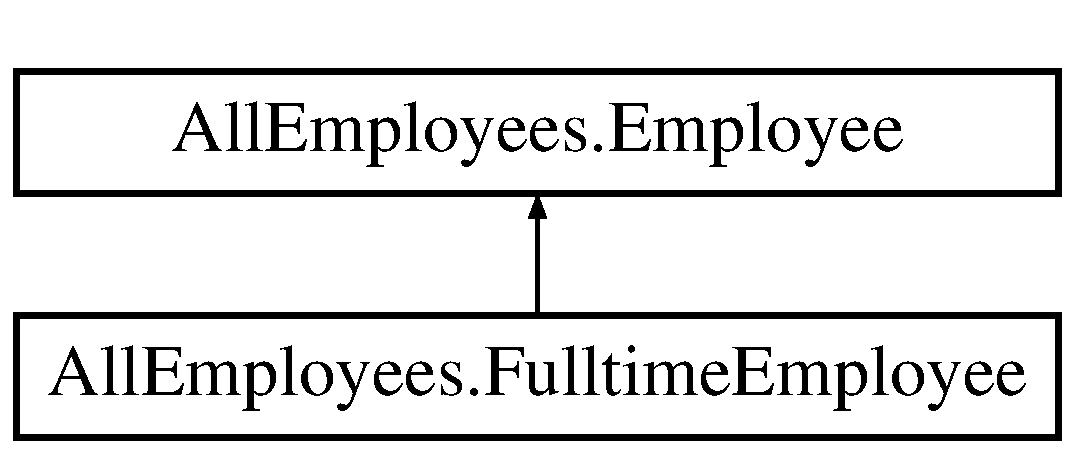
\includegraphics[height=2.000000cm]{class_all_employees_1_1_fulltime_employee}
\end{center}
\end{figure}
\subsection*{Public Member Functions}
\begin{DoxyCompactItemize}
\item 
\hyperlink{class_all_employees_1_1_fulltime_employee_a2f7744fed20aa3161c5ac5cd37c1a281}{Fulltime\+Employee} ()
\begin{DoxyCompactList}\small\item\em default constructor. Sets all values to default \end{DoxyCompactList}\item 
\hyperlink{class_all_employees_1_1_fulltime_employee_a7cc8db6b3e7dd2fa71706c9ebaf68660}{Fulltime\+Employee} (string first\+Name, string last\+Name)
\begin{DoxyCompactList}\small\item\em overloaded constructor. Sets name to inputed names, set all other values to default \end{DoxyCompactList}\item 
\hyperlink{class_all_employees_1_1_fulltime_employee_abf4afc245af7d4d99452ef6251415317}{Fulltime\+Employee} (string first\+Name, string last\+Name, int social\+Insurance\+Number, Date\+Time date\+Of\+Birth, Date\+Time date\+Of\+Hire, Date\+Time date\+Of\+Termination, float salary)
\begin{DoxyCompactList}\small\item\em overloaded constructor. Sets all values to the values given. no default values \end{DoxyCompactList}\item 
bool \hyperlink{class_all_employees_1_1_fulltime_employee_a3e718749e4730c0f2a28f820530071da}{Validate} ()
\begin{DoxyCompactList}\small\item\em Used to determine in the object contains a valid employee. \end{DoxyCompactList}\item 
string \hyperlink{class_all_employees_1_1_fulltime_employee_a7660032e944e78c6ff26598aa7107796}{Details} ()
\begin{DoxyCompactList}\small\item\em Used to print all employee data to the consol. \end{DoxyCompactList}\item 
override string \hyperlink{class_all_employees_1_1_fulltime_employee_a3026e5a4c764fc0da54873cc131e2b82}{To\+String} ()
\begin{DoxyCompactList}\small\item\em Overriden method To\+String used to return a formated string of all data. \end{DoxyCompactList}\item 
bool \hyperlink{class_all_employees_1_1_fulltime_employee_aaf2dc1dcb158819d06958d4399850f56}{Set\+Date\+Of\+Hire} (Date\+Time date)
\begin{DoxyCompactList}\small\item\em Setter for date\+Of\+Hire. \end{DoxyCompactList}\item 
bool \hyperlink{class_all_employees_1_1_fulltime_employee_a6b7516d71f46e650da2200a308d6f226}{Set\+Date\+Of\+Hire} (string date)
\begin{DoxyCompactList}\small\item\em Setter for date\+Of\+Hire from String. \end{DoxyCompactList}\item 
bool \hyperlink{class_all_employees_1_1_fulltime_employee_ae5612c076ead69a3b6f0bbc22a21e293}{Set\+Date\+Of\+Hire} (int year, int month, int day)
\begin{DoxyCompactList}\small\item\em Setter for date\+Of\+Hire from ints. \end{DoxyCompactList}\item 
bool \hyperlink{class_all_employees_1_1_fulltime_employee_a94e9d4b67b20ecbe1449701a200b1c07}{Set\+Date\+Of\+Termination} (Date\+Time date)
\begin{DoxyCompactList}\small\item\em Setter for date\+Of\+Termination. \end{DoxyCompactList}\item 
bool \hyperlink{class_all_employees_1_1_fulltime_employee_a7d142370fe7f81bd623de155a80d0214}{Set\+Date\+Of\+Termination} (string date)
\begin{DoxyCompactList}\small\item\em Setter for date\+Of\+Termination from string. \end{DoxyCompactList}\item 
bool \hyperlink{class_all_employees_1_1_fulltime_employee_aed4ff527256f96b542d0ac0c17f3e2ea}{Set\+Date\+Of\+Termination} (int year, int month, int day)
\begin{DoxyCompactList}\small\item\em Setter for date\+Of\+Termination from int. \end{DoxyCompactList}\item 
bool \hyperlink{class_all_employees_1_1_fulltime_employee_accdd74311a5e97d8beb57d68bd88f95c}{Set\+Salary} (float salary)
\begin{DoxyCompactList}\small\item\em Setter for salary. \end{DoxyCompactList}\item 
Date\+Time \hyperlink{class_all_employees_1_1_fulltime_employee_a3a975ad60176797d1d5529e257596565}{Get\+Date\+Of\+Hire} ()
\begin{DoxyCompactList}\small\item\em Getter for date\+Of\+Hire. \end{DoxyCompactList}\item 
string \hyperlink{class_all_employees_1_1_fulltime_employee_a91b4f15454d92eb7cd33968573050ef0}{Get\+Date\+Of\+Hire\+String} ()
\begin{DoxyCompactList}\small\item\em Getter for date\+Of\+Hire that returns formatted string. \end{DoxyCompactList}\item 
Date\+Time \hyperlink{class_all_employees_1_1_fulltime_employee_a97af3da9151f97e91543d60b6b67a4fa}{Get\+Date\+Of\+Termination} ()
\begin{DoxyCompactList}\small\item\em Getter for date\+Of\+Termination. \end{DoxyCompactList}\item 
string \hyperlink{class_all_employees_1_1_fulltime_employee_a7d0612eba21e83226bb09a174179847c}{Get\+Date\+Of\+Termination\+String} ()
\begin{DoxyCompactList}\small\item\em Getter for date\+Of\+Termination that returns formatted string. \end{DoxyCompactList}\item 
float \hyperlink{class_all_employees_1_1_fulltime_employee_a919105156f70d21baa1f3ce5f4d160ee}{Get\+Salary} ()
\begin{DoxyCompactList}\small\item\em Getter for salary. \end{DoxyCompactList}\end{DoxyCompactItemize}
\subsection*{Private Attributes}
\begin{DoxyCompactItemize}
\item 
\hypertarget{class_all_employees_1_1_fulltime_employee_aa072bd7c652567684c77e0cfd6638af2}{}Date\+Time {\bfseries date\+Of\+Hire}\label{class_all_employees_1_1_fulltime_employee_aa072bd7c652567684c77e0cfd6638af2}

\item 
\hypertarget{class_all_employees_1_1_fulltime_employee_a3836c1a3f74f71f87652c91913eb570c}{}Date\+Time {\bfseries date\+Of\+Termination}\label{class_all_employees_1_1_fulltime_employee_a3836c1a3f74f71f87652c91913eb570c}

\item 
\hypertarget{class_all_employees_1_1_fulltime_employee_afd766110662d0321998cecb84d0dd425}{}float {\bfseries salary}\label{class_all_employees_1_1_fulltime_employee_afd766110662d0321998cecb84d0dd425}

\end{DoxyCompactItemize}
\subsection*{Additional Inherited Members}


\subsection{Detailed Description}
{\bfseries Brief Description} The Fulltime \hyperlink{class_all_employees_1_1_employee}{Employee} class is used to store and manage data about a employee who is hired for a full-\/time position. This class is a child to \hyperlink{class_all_employees_1_1_employee}{Employee} class. It adds the date of hire and termination, and the employees salary. If the constructor creates a invalid employee, a exception is thrown. All other errors result in a defined return. 

\begin{DoxyAuthor}{Author}
{\itshape Brandon} 
\end{DoxyAuthor}


\subsection{Constructor \& Destructor Documentation}
\hypertarget{class_all_employees_1_1_fulltime_employee_a2f7744fed20aa3161c5ac5cd37c1a281}{}\index{All\+Employees\+::\+Fulltime\+Employee@{All\+Employees\+::\+Fulltime\+Employee}!Fulltime\+Employee@{Fulltime\+Employee}}
\index{Fulltime\+Employee@{Fulltime\+Employee}!All\+Employees\+::\+Fulltime\+Employee@{All\+Employees\+::\+Fulltime\+Employee}}
\subsubsection[{Fulltime\+Employee}]{\setlength{\rightskip}{0pt plus 5cm}All\+Employees.\+Fulltime\+Employee.\+Fulltime\+Employee (
\begin{DoxyParamCaption}
{}
\end{DoxyParamCaption}
)}\label{class_all_employees_1_1_fulltime_employee_a2f7744fed20aa3161c5ac5cd37c1a281}


default constructor. Sets all values to default 

{\bfseries Details}


\begin{DoxyParams}{Parameters}
{\em n/a} & \\
\hline
\end{DoxyParams}
\begin{DoxyReturn}{Returns}
n/a 
\end{DoxyReturn}
\hypertarget{class_all_employees_1_1_fulltime_employee_a7cc8db6b3e7dd2fa71706c9ebaf68660}{}\index{All\+Employees\+::\+Fulltime\+Employee@{All\+Employees\+::\+Fulltime\+Employee}!Fulltime\+Employee@{Fulltime\+Employee}}
\index{Fulltime\+Employee@{Fulltime\+Employee}!All\+Employees\+::\+Fulltime\+Employee@{All\+Employees\+::\+Fulltime\+Employee}}
\subsubsection[{Fulltime\+Employee}]{\setlength{\rightskip}{0pt plus 5cm}All\+Employees.\+Fulltime\+Employee.\+Fulltime\+Employee (
\begin{DoxyParamCaption}
\item[{string}]{first\+Name, }
\item[{string}]{last\+Name}
\end{DoxyParamCaption}
)}\label{class_all_employees_1_1_fulltime_employee_a7cc8db6b3e7dd2fa71706c9ebaf68660}


overloaded constructor. Sets name to inputed names, set all other values to default 

{\bfseries Details}


\begin{DoxyParams}{Parameters}
{\em first\+Name} & -\/ {\bfseries string} -\/ First Name of employee to add to records \\
\hline
{\em last\+Name} & -\/ {\bfseries string} -\/ Last Name of employee to add to records\\
\hline
\end{DoxyParams}

\begin{DoxyExceptions}{Exceptions}
{\em $<$\+Failed\+Constructor\+Exception$>$} & -\/ If the constructor failed to create the object\\
\hline
\end{DoxyExceptions}
\begin{DoxyReturn}{Returns}
n/a 
\end{DoxyReturn}
\hypertarget{class_all_employees_1_1_fulltime_employee_abf4afc245af7d4d99452ef6251415317}{}\index{All\+Employees\+::\+Fulltime\+Employee@{All\+Employees\+::\+Fulltime\+Employee}!Fulltime\+Employee@{Fulltime\+Employee}}
\index{Fulltime\+Employee@{Fulltime\+Employee}!All\+Employees\+::\+Fulltime\+Employee@{All\+Employees\+::\+Fulltime\+Employee}}
\subsubsection[{Fulltime\+Employee}]{\setlength{\rightskip}{0pt plus 5cm}All\+Employees.\+Fulltime\+Employee.\+Fulltime\+Employee (
\begin{DoxyParamCaption}
\item[{string}]{first\+Name, }
\item[{string}]{last\+Name, }
\item[{int}]{social\+Insurance\+Number, }
\item[{Date\+Time}]{date\+Of\+Birth, }
\item[{Date\+Time}]{date\+Of\+Hire, }
\item[{Date\+Time}]{date\+Of\+Termination, }
\item[{float}]{salary}
\end{DoxyParamCaption}
)}\label{class_all_employees_1_1_fulltime_employee_abf4afc245af7d4d99452ef6251415317}


overloaded constructor. Sets all values to the values given. no default values 

{\bfseries Details}


\begin{DoxyParams}{Parameters}
{\em first\+Name} & -\/ {\bfseries string} -\/ First Name of employee to add to records \\
\hline
{\em last\+Name} & -\/ {\bfseries string} -\/ Last Name of employee to add to records \\
\hline
{\em social\+Insurance\+Number} & -\/ {\bfseries int} -\/ Social Insurance Number of employee to add to records \\
\hline
{\em date\+Of\+Birth} & -\/ {\bfseries Date\+Time} -\/ Date Of Birth of employee to add to records \\
\hline
{\em date\+Of\+Hire} & -\/ {\bfseries Date\+Time} -\/ Date Of Hire of employee to add to records \\
\hline
{\em date\+Of\+Termination} & -\/ {\bfseries Date\+Time} -\/ Date Of Termination of employee to add to records \\
\hline
{\em salary} & -\/ {\bfseries float} -\/ salary of employee to add to records\\
\hline
\end{DoxyParams}

\begin{DoxyExceptions}{Exceptions}
{\em $<$\+Failed\+Constructor\+Exception$>$} & -\/ If the constructor failed to create the object\\
\hline
\end{DoxyExceptions}
\begin{DoxyReturn}{Returns}
n/a 
\end{DoxyReturn}


\subsection{Member Function Documentation}
\hypertarget{class_all_employees_1_1_fulltime_employee_a7660032e944e78c6ff26598aa7107796}{}\index{All\+Employees\+::\+Fulltime\+Employee@{All\+Employees\+::\+Fulltime\+Employee}!Details@{Details}}
\index{Details@{Details}!All\+Employees\+::\+Fulltime\+Employee@{All\+Employees\+::\+Fulltime\+Employee}}
\subsubsection[{Details}]{\setlength{\rightskip}{0pt plus 5cm}string All\+Employees.\+Fulltime\+Employee.\+Details (
\begin{DoxyParamCaption}
{}
\end{DoxyParamCaption}
)}\label{class_all_employees_1_1_fulltime_employee_a7660032e944e78c6ff26598aa7107796}


Used to print all employee data to the consol. 

{\bfseries Details}


\begin{DoxyParams}{Parameters}
{\em n/a} & \\
\hline
\end{DoxyParams}
\begin{DoxyReturn}{Returns}
user\+Info {\bfseries string} -\/ formatted string of employee data 
\end{DoxyReturn}
\hypertarget{class_all_employees_1_1_fulltime_employee_a3a975ad60176797d1d5529e257596565}{}\index{All\+Employees\+::\+Fulltime\+Employee@{All\+Employees\+::\+Fulltime\+Employee}!Get\+Date\+Of\+Hire@{Get\+Date\+Of\+Hire}}
\index{Get\+Date\+Of\+Hire@{Get\+Date\+Of\+Hire}!All\+Employees\+::\+Fulltime\+Employee@{All\+Employees\+::\+Fulltime\+Employee}}
\subsubsection[{Get\+Date\+Of\+Hire}]{\setlength{\rightskip}{0pt plus 5cm}Date\+Time All\+Employees.\+Fulltime\+Employee.\+Get\+Date\+Of\+Hire (
\begin{DoxyParamCaption}
{}
\end{DoxyParamCaption}
)}\label{class_all_employees_1_1_fulltime_employee_a3a975ad60176797d1d5529e257596565}


Getter for date\+Of\+Hire. 

{\bfseries Details}


\begin{DoxyParams}{Parameters}
{\em n/a} & \\
\hline
\end{DoxyParams}
\begin{DoxyReturn}{Returns}
date\+Of\+Hire {\bfseries Date\+Time} 
\end{DoxyReturn}
\hypertarget{class_all_employees_1_1_fulltime_employee_a91b4f15454d92eb7cd33968573050ef0}{}\index{All\+Employees\+::\+Fulltime\+Employee@{All\+Employees\+::\+Fulltime\+Employee}!Get\+Date\+Of\+Hire\+String@{Get\+Date\+Of\+Hire\+String}}
\index{Get\+Date\+Of\+Hire\+String@{Get\+Date\+Of\+Hire\+String}!All\+Employees\+::\+Fulltime\+Employee@{All\+Employees\+::\+Fulltime\+Employee}}
\subsubsection[{Get\+Date\+Of\+Hire\+String}]{\setlength{\rightskip}{0pt plus 5cm}string All\+Employees.\+Fulltime\+Employee.\+Get\+Date\+Of\+Hire\+String (
\begin{DoxyParamCaption}
{}
\end{DoxyParamCaption}
)}\label{class_all_employees_1_1_fulltime_employee_a91b4f15454d92eb7cd33968573050ef0}


Getter for date\+Of\+Hire that returns formatted string. 

{\bfseries Details}


\begin{DoxyParams}{Parameters}
{\em n/a} & \\
\hline
\end{DoxyParams}
\begin{DoxyReturn}{Returns}
date\+Of\+Hire {\bfseries string} 
\end{DoxyReturn}
\hypertarget{class_all_employees_1_1_fulltime_employee_a97af3da9151f97e91543d60b6b67a4fa}{}\index{All\+Employees\+::\+Fulltime\+Employee@{All\+Employees\+::\+Fulltime\+Employee}!Get\+Date\+Of\+Termination@{Get\+Date\+Of\+Termination}}
\index{Get\+Date\+Of\+Termination@{Get\+Date\+Of\+Termination}!All\+Employees\+::\+Fulltime\+Employee@{All\+Employees\+::\+Fulltime\+Employee}}
\subsubsection[{Get\+Date\+Of\+Termination}]{\setlength{\rightskip}{0pt plus 5cm}Date\+Time All\+Employees.\+Fulltime\+Employee.\+Get\+Date\+Of\+Termination (
\begin{DoxyParamCaption}
{}
\end{DoxyParamCaption}
)}\label{class_all_employees_1_1_fulltime_employee_a97af3da9151f97e91543d60b6b67a4fa}


Getter for date\+Of\+Termination. 

{\bfseries Details}


\begin{DoxyParams}{Parameters}
{\em n/a} & \\
\hline
\end{DoxyParams}
\begin{DoxyReturn}{Returns}
date\+Of\+Termination {\bfseries Date\+Time} 
\end{DoxyReturn}
\hypertarget{class_all_employees_1_1_fulltime_employee_a7d0612eba21e83226bb09a174179847c}{}\index{All\+Employees\+::\+Fulltime\+Employee@{All\+Employees\+::\+Fulltime\+Employee}!Get\+Date\+Of\+Termination\+String@{Get\+Date\+Of\+Termination\+String}}
\index{Get\+Date\+Of\+Termination\+String@{Get\+Date\+Of\+Termination\+String}!All\+Employees\+::\+Fulltime\+Employee@{All\+Employees\+::\+Fulltime\+Employee}}
\subsubsection[{Get\+Date\+Of\+Termination\+String}]{\setlength{\rightskip}{0pt plus 5cm}string All\+Employees.\+Fulltime\+Employee.\+Get\+Date\+Of\+Termination\+String (
\begin{DoxyParamCaption}
{}
\end{DoxyParamCaption}
)}\label{class_all_employees_1_1_fulltime_employee_a7d0612eba21e83226bb09a174179847c}


Getter for date\+Of\+Termination that returns formatted string. 

{\bfseries Details}


\begin{DoxyParams}{Parameters}
{\em n/a} & \\
\hline
\end{DoxyParams}
\begin{DoxyReturn}{Returns}
date\+Of\+Termination {\bfseries string} 
\end{DoxyReturn}
\hypertarget{class_all_employees_1_1_fulltime_employee_a919105156f70d21baa1f3ce5f4d160ee}{}\index{All\+Employees\+::\+Fulltime\+Employee@{All\+Employees\+::\+Fulltime\+Employee}!Get\+Salary@{Get\+Salary}}
\index{Get\+Salary@{Get\+Salary}!All\+Employees\+::\+Fulltime\+Employee@{All\+Employees\+::\+Fulltime\+Employee}}
\subsubsection[{Get\+Salary}]{\setlength{\rightskip}{0pt plus 5cm}float All\+Employees.\+Fulltime\+Employee.\+Get\+Salary (
\begin{DoxyParamCaption}
{}
\end{DoxyParamCaption}
)}\label{class_all_employees_1_1_fulltime_employee_a919105156f70d21baa1f3ce5f4d160ee}


Getter for salary. 

{\bfseries Details}


\begin{DoxyParams}{Parameters}
{\em n/a} & \\
\hline
\end{DoxyParams}
\begin{DoxyReturn}{Returns}
salary {\bfseries float} 
\end{DoxyReturn}
\hypertarget{class_all_employees_1_1_fulltime_employee_aaf2dc1dcb158819d06958d4399850f56}{}\index{All\+Employees\+::\+Fulltime\+Employee@{All\+Employees\+::\+Fulltime\+Employee}!Set\+Date\+Of\+Hire@{Set\+Date\+Of\+Hire}}
\index{Set\+Date\+Of\+Hire@{Set\+Date\+Of\+Hire}!All\+Employees\+::\+Fulltime\+Employee@{All\+Employees\+::\+Fulltime\+Employee}}
\subsubsection[{Set\+Date\+Of\+Hire}]{\setlength{\rightskip}{0pt plus 5cm}bool All\+Employees.\+Fulltime\+Employee.\+Set\+Date\+Of\+Hire (
\begin{DoxyParamCaption}
\item[{Date\+Time}]{date}
\end{DoxyParamCaption}
)}\label{class_all_employees_1_1_fulltime_employee_aaf2dc1dcb158819d06958d4399850f56}


Setter for date\+Of\+Hire. 

{\bfseries Details}


\begin{DoxyParams}{Parameters}
{\em date} & {\bfseries Date\+Time} -\/ The employees date of hire\\
\hline
\end{DoxyParams}
\begin{DoxyReturn}{Returns}
data\+Saved {\bfseries bool} -\/ true if input was valid and data was changed. False it data was not changed 
\end{DoxyReturn}
\hypertarget{class_all_employees_1_1_fulltime_employee_a6b7516d71f46e650da2200a308d6f226}{}\index{All\+Employees\+::\+Fulltime\+Employee@{All\+Employees\+::\+Fulltime\+Employee}!Set\+Date\+Of\+Hire@{Set\+Date\+Of\+Hire}}
\index{Set\+Date\+Of\+Hire@{Set\+Date\+Of\+Hire}!All\+Employees\+::\+Fulltime\+Employee@{All\+Employees\+::\+Fulltime\+Employee}}
\subsubsection[{Set\+Date\+Of\+Hire}]{\setlength{\rightskip}{0pt plus 5cm}bool All\+Employees.\+Fulltime\+Employee.\+Set\+Date\+Of\+Hire (
\begin{DoxyParamCaption}
\item[{string}]{date}
\end{DoxyParamCaption}
)}\label{class_all_employees_1_1_fulltime_employee_a6b7516d71f46e650da2200a308d6f226}


Setter for date\+Of\+Hire from String. 

{\bfseries Details}


\begin{DoxyParams}{Parameters}
{\em date} & {\bfseries string} -\/ The employees date of hire\\
\hline
\end{DoxyParams}
\begin{DoxyReturn}{Returns}
data\+Saved {\bfseries bool} -\/ true if input was valid and data was changed. False it data was not changed 
\end{DoxyReturn}
\hypertarget{class_all_employees_1_1_fulltime_employee_ae5612c076ead69a3b6f0bbc22a21e293}{}\index{All\+Employees\+::\+Fulltime\+Employee@{All\+Employees\+::\+Fulltime\+Employee}!Set\+Date\+Of\+Hire@{Set\+Date\+Of\+Hire}}
\index{Set\+Date\+Of\+Hire@{Set\+Date\+Of\+Hire}!All\+Employees\+::\+Fulltime\+Employee@{All\+Employees\+::\+Fulltime\+Employee}}
\subsubsection[{Set\+Date\+Of\+Hire}]{\setlength{\rightskip}{0pt plus 5cm}bool All\+Employees.\+Fulltime\+Employee.\+Set\+Date\+Of\+Hire (
\begin{DoxyParamCaption}
\item[{int}]{year, }
\item[{int}]{month, }
\item[{int}]{day}
\end{DoxyParamCaption}
)}\label{class_all_employees_1_1_fulltime_employee_ae5612c076ead69a3b6f0bbc22a21e293}


Setter for date\+Of\+Hire from ints. 

{\bfseries Details}


\begin{DoxyParams}{Parameters}
{\em year} & {\bfseries int} -\/ The start year of the employees date of hire \\
\hline
{\em month} & {\bfseries int} -\/ The start month of the employees date of hire \\
\hline
{\em day} & {\bfseries int} -\/ The start day of the employees date of hire\\
\hline
\end{DoxyParams}
\begin{DoxyReturn}{Returns}
data\+Saved {\bfseries bool} -\/ true if input was valid and data was changed. False it data was not changed 
\end{DoxyReturn}
\hypertarget{class_all_employees_1_1_fulltime_employee_a94e9d4b67b20ecbe1449701a200b1c07}{}\index{All\+Employees\+::\+Fulltime\+Employee@{All\+Employees\+::\+Fulltime\+Employee}!Set\+Date\+Of\+Termination@{Set\+Date\+Of\+Termination}}
\index{Set\+Date\+Of\+Termination@{Set\+Date\+Of\+Termination}!All\+Employees\+::\+Fulltime\+Employee@{All\+Employees\+::\+Fulltime\+Employee}}
\subsubsection[{Set\+Date\+Of\+Termination}]{\setlength{\rightskip}{0pt plus 5cm}bool All\+Employees.\+Fulltime\+Employee.\+Set\+Date\+Of\+Termination (
\begin{DoxyParamCaption}
\item[{Date\+Time}]{date}
\end{DoxyParamCaption}
)}\label{class_all_employees_1_1_fulltime_employee_a94e9d4b67b20ecbe1449701a200b1c07}


Setter for date\+Of\+Termination. 

{\bfseries Details}


\begin{DoxyParams}{Parameters}
{\em date} & {\bfseries Date\+Time} -\/ The employees date of termination\\
\hline
\end{DoxyParams}
\begin{DoxyReturn}{Returns}
data\+Saved {\bfseries bool} -\/ true if input was valid and data was changed. False it data was not changed 
\end{DoxyReturn}
\hypertarget{class_all_employees_1_1_fulltime_employee_a7d142370fe7f81bd623de155a80d0214}{}\index{All\+Employees\+::\+Fulltime\+Employee@{All\+Employees\+::\+Fulltime\+Employee}!Set\+Date\+Of\+Termination@{Set\+Date\+Of\+Termination}}
\index{Set\+Date\+Of\+Termination@{Set\+Date\+Of\+Termination}!All\+Employees\+::\+Fulltime\+Employee@{All\+Employees\+::\+Fulltime\+Employee}}
\subsubsection[{Set\+Date\+Of\+Termination}]{\setlength{\rightskip}{0pt plus 5cm}bool All\+Employees.\+Fulltime\+Employee.\+Set\+Date\+Of\+Termination (
\begin{DoxyParamCaption}
\item[{string}]{date}
\end{DoxyParamCaption}
)}\label{class_all_employees_1_1_fulltime_employee_a7d142370fe7f81bd623de155a80d0214}


Setter for date\+Of\+Termination from string. 

{\bfseries Details}


\begin{DoxyParams}{Parameters}
{\em date} & {\bfseries string} -\/ The employees date of termination\\
\hline
\end{DoxyParams}
\begin{DoxyReturn}{Returns}
data\+Saved {\bfseries bool} -\/ true if input was valid and data was changed. False it data was not changed 
\end{DoxyReturn}
\hypertarget{class_all_employees_1_1_fulltime_employee_aed4ff527256f96b542d0ac0c17f3e2ea}{}\index{All\+Employees\+::\+Fulltime\+Employee@{All\+Employees\+::\+Fulltime\+Employee}!Set\+Date\+Of\+Termination@{Set\+Date\+Of\+Termination}}
\index{Set\+Date\+Of\+Termination@{Set\+Date\+Of\+Termination}!All\+Employees\+::\+Fulltime\+Employee@{All\+Employees\+::\+Fulltime\+Employee}}
\subsubsection[{Set\+Date\+Of\+Termination}]{\setlength{\rightskip}{0pt plus 5cm}bool All\+Employees.\+Fulltime\+Employee.\+Set\+Date\+Of\+Termination (
\begin{DoxyParamCaption}
\item[{int}]{year, }
\item[{int}]{month, }
\item[{int}]{day}
\end{DoxyParamCaption}
)}\label{class_all_employees_1_1_fulltime_employee_aed4ff527256f96b542d0ac0c17f3e2ea}


Setter for date\+Of\+Termination from int. 

{\bfseries Details}


\begin{DoxyParams}{Parameters}
{\em year} & {\bfseries int} -\/ The start year of the employees date of termination \\
\hline
{\em month} & {\bfseries int} -\/ The start month of the employees date of termination \\
\hline
{\em day} & {\bfseries int} -\/ The start day of the employees date of termination\\
\hline
\end{DoxyParams}
\begin{DoxyReturn}{Returns}
data\+Saved {\bfseries bool} -\/ true if input was valid and data was changed. False it data was not changed 
\end{DoxyReturn}
\hypertarget{class_all_employees_1_1_fulltime_employee_accdd74311a5e97d8beb57d68bd88f95c}{}\index{All\+Employees\+::\+Fulltime\+Employee@{All\+Employees\+::\+Fulltime\+Employee}!Set\+Salary@{Set\+Salary}}
\index{Set\+Salary@{Set\+Salary}!All\+Employees\+::\+Fulltime\+Employee@{All\+Employees\+::\+Fulltime\+Employee}}
\subsubsection[{Set\+Salary}]{\setlength{\rightskip}{0pt plus 5cm}bool All\+Employees.\+Fulltime\+Employee.\+Set\+Salary (
\begin{DoxyParamCaption}
\item[{float}]{salary}
\end{DoxyParamCaption}
)}\label{class_all_employees_1_1_fulltime_employee_accdd74311a5e97d8beb57d68bd88f95c}


Setter for salary. 

{\bfseries Details}


\begin{DoxyParams}{Parameters}
{\em salary} & {\bfseries float} -\/ The salary of the employee\\
\hline
\end{DoxyParams}
\begin{DoxyReturn}{Returns}
data\+Saved {\bfseries bool} -\/ true if input was valid and data was changed. False it data was not changed 
\end{DoxyReturn}
\hypertarget{class_all_employees_1_1_fulltime_employee_a3026e5a4c764fc0da54873cc131e2b82}{}\index{All\+Employees\+::\+Fulltime\+Employee@{All\+Employees\+::\+Fulltime\+Employee}!To\+String@{To\+String}}
\index{To\+String@{To\+String}!All\+Employees\+::\+Fulltime\+Employee@{All\+Employees\+::\+Fulltime\+Employee}}
\subsubsection[{To\+String}]{\setlength{\rightskip}{0pt plus 5cm}override string All\+Employees.\+Fulltime\+Employee.\+To\+String (
\begin{DoxyParamCaption}
{}
\end{DoxyParamCaption}
)}\label{class_all_employees_1_1_fulltime_employee_a3026e5a4c764fc0da54873cc131e2b82}


Overriden method To\+String used to return a formated string of all data. 

{\bfseries Details}


\begin{DoxyParams}{Parameters}
{\em n/a} & \\
\hline
\end{DoxyParams}
\begin{DoxyReturn}{Returns}
employee\+String {\bfseries string} -\/ the formated string containing all employee data 
\end{DoxyReturn}
\hypertarget{class_all_employees_1_1_fulltime_employee_a3e718749e4730c0f2a28f820530071da}{}\index{All\+Employees\+::\+Fulltime\+Employee@{All\+Employees\+::\+Fulltime\+Employee}!Validate@{Validate}}
\index{Validate@{Validate}!All\+Employees\+::\+Fulltime\+Employee@{All\+Employees\+::\+Fulltime\+Employee}}
\subsubsection[{Validate}]{\setlength{\rightskip}{0pt plus 5cm}bool All\+Employees.\+Fulltime\+Employee.\+Validate (
\begin{DoxyParamCaption}
{}
\end{DoxyParamCaption}
)}\label{class_all_employees_1_1_fulltime_employee_a3e718749e4730c0f2a28f820530071da}


Used to determine in the object contains a valid employee. 

{\bfseries Details}


\begin{DoxyParams}{Parameters}
{\em n/a} & \\
\hline
\end{DoxyParams}
\begin{DoxyReturn}{Returns}
data\+Valid -\/ {\bfseries bool} -\/ True if the object contains all data for a valid employee 
\end{DoxyReturn}


The documentation for this class was generated from the following file\+:\begin{DoxyCompactItemize}
\item 
C\+:/\+S\+E\+T\+Repo/trunk/\+E\+M\+S/trunk/\+All\+Employees/\+All\+Employees/Fulltime\+Employee.\+cs\end{DoxyCompactItemize}

\hypertarget{class_my_all_employee_1_1_tests_1_1_full_time_employee_tests}{}\section{My\+All\+Employee.\+Tests.\+Full\+Time\+Employee\+Tests Class Reference}
\label{class_my_all_employee_1_1_tests_1_1_full_time_employee_tests}\index{My\+All\+Employee.\+Tests.\+Full\+Time\+Employee\+Tests@{My\+All\+Employee.\+Tests.\+Full\+Time\+Employee\+Tests}}


{\bfseries  Brief Description} This class is used to test the Fulltime\+Employee methods in the All\+Employee class. The methods tested include the constructors, Details, Set\+Date\+Of\+Birth (all 3 overloaded methods), Set\+Dateof\+Hire (all 3 overloaded methods), Set\+Dateof\+Termination(all 3 overloaded methods), Set\+Salary and To\+String.  


\subsection*{Public Member Functions}
\begin{DoxyCompactItemize}
\item 
void \hyperlink{class_my_all_employee_1_1_tests_1_1_full_time_employee_tests_aff1bdc7a8fa9aff78fb90649f0387306}{Constructor\+With\+Names\+Test\+Valid1} ()
\begin{DoxyCompactList}\small\item\em This unit test will check if either name contains anything other than a letter, apostrophe, dash. It will throw an exception if wrong. \end{DoxyCompactList}\item 
void \hyperlink{class_my_all_employee_1_1_tests_1_1_full_time_employee_tests_aa387aed7c291d9bbaa319ab5bb190080}{Constructor\+With\+Names\+Test\+Valid2} ()
\begin{DoxyCompactList}\small\item\em This unit test will check if either name contains anything other than a letter, apostrophe, dash. It will throw an exception if wrong. \end{DoxyCompactList}\item 
void \hyperlink{class_my_all_employee_1_1_tests_1_1_full_time_employee_tests_aafea43d4b6fc4792bae0eb1de0774199}{Constructor\+With\+Names\+Test\+Valid3} ()
\begin{DoxyCompactList}\small\item\em This unit test will check if either name contains anything other than a letter, apostrophe, dash. It will throw an exception if wrong. \end{DoxyCompactList}\item 
void \hyperlink{class_my_all_employee_1_1_tests_1_1_full_time_employee_tests_ad496f29cdf84e7ffce7cfe71da86df73}{Constructor\+With\+Names\+Test\+Invalid\+Slash} ()
\begin{DoxyCompactList}\small\item\em This unit test will check if the constructor will fail and if the string is invalid because it contains a slash. \end{DoxyCompactList}\item 
void \hyperlink{class_my_all_employee_1_1_tests_1_1_full_time_employee_tests_ab4cffc36ebfb317368cc227023925a2d}{Constructor\+With\+Names\+Test\+Invalid\+Space} ()
\begin{DoxyCompactList}\small\item\em This unit test will check if the constructor will fail and if the string is invalid because it contains a space. \end{DoxyCompactList}\item 
void \hyperlink{class_my_all_employee_1_1_tests_1_1_full_time_employee_tests_aeb693bf7d723b3093207cd16dfe67922}{Constructor\+With\+Names\+Test\+Invalid\+Number} ()
\begin{DoxyCompactList}\small\item\em This unit test will check if the constructor will fail and if the string is invalid because it contains a number. \end{DoxyCompactList}\item 
void \hyperlink{class_my_all_employee_1_1_tests_1_1_full_time_employee_tests_ad46719ac401ed4233b120609fa057374}{Constructor\+With\+All\+Param\+Test\+Valid1} ()
\begin{DoxyCompactList}\small\item\em This unit test will check the constructor that takes in all possible parameters, and give them all valid data. \end{DoxyCompactList}\item 
void \hyperlink{class_my_all_employee_1_1_tests_1_1_full_time_employee_tests_a3fe215b36ca6d6928beeb8fe9b86d706}{Constructor\+With\+All\+Param\+Test\+Valid2} ()
\begin{DoxyCompactList}\small\item\em This unit test will check the constructor that takes in all possible parameters, and give them all valid data. \end{DoxyCompactList}\item 
void \hyperlink{class_my_all_employee_1_1_tests_1_1_full_time_employee_tests_af5a3ab06211fa668ac9a00cc160961be}{Constructor\+With\+All\+Param\+Test\+Valid3} ()
\begin{DoxyCompactList}\small\item\em This unit test will check the constructor that takes in all possible parameters, and give them all valid data. \end{DoxyCompactList}\item 
void \hyperlink{class_my_all_employee_1_1_tests_1_1_full_time_employee_tests_af5d09cc6cc90ec01183f059f12ef04f7}{Constructor\+With\+All\+Param\+Test\+Invalid\+S\+I\+N} ()
\begin{DoxyCompactList}\small\item\em This unit test will check the constructor that takes in all possible parameters, and give them all invalid data. \end{DoxyCompactList}\item 
void \hyperlink{class_my_all_employee_1_1_tests_1_1_full_time_employee_tests_a49b3d396694536945d39f2f56c8e2ffc}{Constructor\+With\+All\+Param\+Test\+Invalid\+D\+O\+H\+Before\+D\+O\+B} ()
\begin{DoxyCompactList}\small\item\em This unit test will check the constructor that takes in all possible parameters, and give them all invalid data. \end{DoxyCompactList}\item 
void \hyperlink{class_my_all_employee_1_1_tests_1_1_full_time_employee_tests_af86e639c0ad8ddb950f32c10d0aef18b}{Constructor\+With\+All\+Param\+Test\+Invalid\+D\+O\+T\+Bofore\+D\+O\+H} ()
\begin{DoxyCompactList}\small\item\em This unit test will check the constructor that takes in all possible parameters, and give them all invalid data. \end{DoxyCompactList}\item 
void \hyperlink{class_my_all_employee_1_1_tests_1_1_full_time_employee_tests_ab76d68d6df376b1ec8694cba60b2ed96}{Constructor\+With\+All\+Param\+Test\+Invalid\+D\+O\+Tno\+D\+O\+H} ()
\begin{DoxyCompactList}\small\item\em This unit test will check the constructor that takes in all possible parameters, and give them all invalid data. \end{DoxyCompactList}\item 
void \hyperlink{class_my_all_employee_1_1_tests_1_1_full_time_employee_tests_a59450e7f9d9a9dd87710623acd826566}{Details\+Test\+Valid} ()
\begin{DoxyCompactList}\small\item\em This unit test will create an employee and runs it\textquotesingle{}s details, and will ensure that the string is what it should be(it is hardcoded) \end{DoxyCompactList}\item 
void \hyperlink{class_my_all_employee_1_1_tests_1_1_full_time_employee_tests_a06a5cef67c7ba190e9dc07902aaf4f76}{To\+String\+Test\+Valid} ()
\begin{DoxyCompactList}\small\item\em This unit test will create an employee and runs it\textquotesingle{}s details, and will ensure that the string is what it should be(it is hardcoded) \end{DoxyCompactList}\item 
void \hyperlink{class_my_all_employee_1_1_tests_1_1_full_time_employee_tests_a608fd7d42e10fb6da5f03150b3f4a96b}{Set\+Date\+Of\+Birth\+Date\+Test\+Valid\+Date} ()
\begin{DoxyCompactList}\small\item\em This unit test will set the birth date to a valid date. \end{DoxyCompactList}\item 
void \hyperlink{class_my_all_employee_1_1_tests_1_1_full_time_employee_tests_a55349b1b82a2fa2317cfc5264117c39b}{Set\+Date\+Of\+Birth\+Date\+Test\+Invalid\+D\+O\+Bafter\+D\+O\+H} ()
\begin{DoxyCompactList}\small\item\em This unit test will set the birth date to an invalid date. \end{DoxyCompactList}\item 
void \hyperlink{class_my_all_employee_1_1_tests_1_1_full_time_employee_tests_a67f757b32c290ae433884bce57e33654}{Set\+Date\+Of\+Birth\+String\+Test\+Valid\+String} ()
\begin{DoxyCompactList}\small\item\em This unit test will set the birth string to a valid string. \end{DoxyCompactList}\item 
void \hyperlink{class_my_all_employee_1_1_tests_1_1_full_time_employee_tests_acea46d71cc386e8f83ec2d8d14e2e0ba}{Set\+Date\+Of\+Birth\+String\+Test\+Invalid\+Format} ()
\begin{DoxyCompactList}\small\item\em This unit test will set the birth string to an invalid string. \end{DoxyCompactList}\item 
void \hyperlink{class_my_all_employee_1_1_tests_1_1_full_time_employee_tests_a42006f31a8eef0684f11d335ce47d8c8}{Set\+Date\+Of\+Birth\+String\+Test\+Invalid\+Date} ()
\begin{DoxyCompactList}\small\item\em This unit test will set the birth string to an invalid string. \end{DoxyCompactList}\item 
void \hyperlink{class_my_all_employee_1_1_tests_1_1_full_time_employee_tests_a41513d1b83b5cc8380c5cd19d0ef45d7}{Set\+Date\+Of\+Birth\+String\+Test\+Invalid\+Future} ()
\begin{DoxyCompactList}\small\item\em This unit test will set the birth string to an invalid string. \end{DoxyCompactList}\item 
void \hyperlink{class_my_all_employee_1_1_tests_1_1_full_time_employee_tests_accc07c2a05da5a5c28d570cfc8a90bda}{Set\+Date\+Of\+Birth\+String\+Test\+Invalid\+D\+O\+Bafter\+D\+O\+H} ()
\begin{DoxyCompactList}\small\item\em This unit test will set the birth string to an invalid string. \end{DoxyCompactList}\item 
void \hyperlink{class_my_all_employee_1_1_tests_1_1_full_time_employee_tests_a3f3d2617612859580d5dc47389eb1123}{Set\+Date\+Of\+Birth\+Ints\+Test\+Invalid\+Letter} ()
\begin{DoxyCompactList}\small\item\em This unit test will set the birth date to an invalid date. \end{DoxyCompactList}\item 
void \hyperlink{class_my_all_employee_1_1_tests_1_1_full_time_employee_tests_a41a49bd14578bcfdbf5b0f5a8a5736d6}{Set\+Date\+Of\+Birth\+Ints\+Test\+Valid} ()
\begin{DoxyCompactList}\small\item\em This unit test will set the birth date to a valid date. \end{DoxyCompactList}\item 
void \hyperlink{class_my_all_employee_1_1_tests_1_1_full_time_employee_tests_a3fa32eaeed78ad324b486fbfa551ad5a}{Set\+Date\+Of\+Birth\+Ints\+Test\+Invalid\+Date} ()
\begin{DoxyCompactList}\small\item\em This unit test will set the birth date to an invalid date. \end{DoxyCompactList}\item 
void \hyperlink{class_my_all_employee_1_1_tests_1_1_full_time_employee_tests_ad5818f2cc909a75875463cc5c1ffd7ec}{Set\+Date\+Of\+Birth\+Ints\+Test\+Invalid\+Future\+Date} ()
\begin{DoxyCompactList}\small\item\em This unit test will set the birth date to an invalid date. \end{DoxyCompactList}\item 
void \hyperlink{class_my_all_employee_1_1_tests_1_1_full_time_employee_tests_af7750b640456bbea7ebd909f992dc71c}{Set\+Date\+Of\+Birth\+Ints\+Test\+Invalid\+D\+O\+Bafter\+D\+O\+H} ()
\begin{DoxyCompactList}\small\item\em This unit test will set the birth date to an invalid date. \end{DoxyCompactList}\item 
void \hyperlink{class_my_all_employee_1_1_tests_1_1_full_time_employee_tests_a40c32764494bedbe96dcc6770a853f4e}{Set\+Date\+Of\+Hire\+Date\+Test\+Valid\+Date} ()
\begin{DoxyCompactList}\small\item\em This unit test will set the date of hire date to a valid date. \end{DoxyCompactList}\item 
void \hyperlink{class_my_all_employee_1_1_tests_1_1_full_time_employee_tests_a08e1fe6af4086293b66b5646cef6f712}{Set\+Date\+Of\+Hire\+Date\+Test\+Invalid\+D\+O\+Hafter\+D\+O\+T} ()
\begin{DoxyCompactList}\small\item\em This unit test will set the date of hire date to an invalid date. \end{DoxyCompactList}\item 
void \hyperlink{class_my_all_employee_1_1_tests_1_1_full_time_employee_tests_aebed253ddcbbee1853a6b967c93d6257}{Set\+Date\+Of\+Hire\+String\+Test\+Invalid\+D\+O\+Hbefore\+D\+O\+B} ()
\begin{DoxyCompactList}\small\item\em This unit test will set the date of hire string to an invalid string. \end{DoxyCompactList}\item 
void \hyperlink{class_my_all_employee_1_1_tests_1_1_full_time_employee_tests_a2832cf212d439622e5cd3764771c1bc4}{Set\+Date\+Of\+Hire\+String\+Test\+Valid\+String} ()
\begin{DoxyCompactList}\small\item\em This unit test will set the date of hire string to a valid string. \end{DoxyCompactList}\item 
void \hyperlink{class_my_all_employee_1_1_tests_1_1_full_time_employee_tests_a9cdc68100bbbf4e8deb270b9b63e718a}{Set\+Date\+Of\+Hire\+String\+Test\+Invalid\+Format} ()
\begin{DoxyCompactList}\small\item\em This unit test will set the date of hire string to an invalid string. \end{DoxyCompactList}\item 
void \hyperlink{class_my_all_employee_1_1_tests_1_1_full_time_employee_tests_ad6ce9c3cfd0b1970fbc8f616c40ca52d}{Set\+Date\+Of\+Hire\+String\+Test\+Invalid\+Date} ()
\begin{DoxyCompactList}\small\item\em This unit test will set the date of hire string to an invalid string. \end{DoxyCompactList}\item 
void \hyperlink{class_my_all_employee_1_1_tests_1_1_full_time_employee_tests_a6d27a8759d55854878fb6b8a00b8e7dc}{Set\+Date\+Of\+Hire\+String\+Test\+Invalid\+D\+O\+Hafter\+D\+O\+T} ()
\begin{DoxyCompactList}\small\item\em This unit test will set the date of hire string to an invalid string. \end{DoxyCompactList}\item 
void \hyperlink{class_my_all_employee_1_1_tests_1_1_full_time_employee_tests_a40aa8631bb91216a166885c55a65c506}{Set\+Date\+Of\+Hire\+Date\+Test\+Invalid\+D\+O\+Hbefore\+D\+O\+B} ()
\begin{DoxyCompactList}\small\item\em This unit test will set the date of hire date to an invalid date. \end{DoxyCompactList}\item 
void \hyperlink{class_my_all_employee_1_1_tests_1_1_full_time_employee_tests_a8db2a2084aa12703dde58c9dcf8d0ece}{Set\+Date\+Of\+Hire\+Ints\+Test\+Invalid\+Letter} ()
\begin{DoxyCompactList}\small\item\em This unit test will set the date of hire date to an invalid date. \end{DoxyCompactList}\item 
void \hyperlink{class_my_all_employee_1_1_tests_1_1_full_time_employee_tests_a45b2e90d3fed9ea7f7eec3c805e29972}{Set\+Date\+Of\+Hire\+Ints\+Test\+Valid} ()
\begin{DoxyCompactList}\small\item\em This unit test will set the date of hire date to a valid date. \end{DoxyCompactList}\item 
void \hyperlink{class_my_all_employee_1_1_tests_1_1_full_time_employee_tests_a74c777c5bac2bbd565153427beb75f3d}{Set\+Date\+Of\+Hire\+Ints\+Test\+Invalid\+Date} ()
\begin{DoxyCompactList}\small\item\em This unit test will set the date of hire date to an invalid date. \end{DoxyCompactList}\item 
void \hyperlink{class_my_all_employee_1_1_tests_1_1_full_time_employee_tests_a113325a9cea1175e54bf6a27a725f2f3}{Set\+Date\+Of\+Hire\+Ints\+Test\+Invalid\+D\+O\+Hafter\+D\+O\+T} ()
\begin{DoxyCompactList}\small\item\em This unit test will set the date of hire date to an invalid date. \end{DoxyCompactList}\item 
void \hyperlink{class_my_all_employee_1_1_tests_1_1_full_time_employee_tests_abed90ce94167001c8dd5957d7e898078}{Set\+Date\+Of\+Hire\+Ints\+Test\+Invalid\+D\+O\+Hbefore\+D\+O\+B} ()
\begin{DoxyCompactList}\small\item\em This unit test will set the date of hire date to an invalid date. \end{DoxyCompactList}\item 
void \hyperlink{class_my_all_employee_1_1_tests_1_1_full_time_employee_tests_a763d6c3bcda0733dc7d575f934f941fb}{Set\+Date\+Of\+Termination\+Date\+Test\+Valid\+Date} ()
\begin{DoxyCompactList}\small\item\em This unit test will set the date of termination date to a valid date. \end{DoxyCompactList}\item 
void \hyperlink{class_my_all_employee_1_1_tests_1_1_full_time_employee_tests_afa99fad6c7ea636ea1f96c503287ff02}{Set\+Date\+Of\+Termination\+Date\+Test\+Invalid\+D\+O\+Tbefore\+D\+O\+H} ()
\begin{DoxyCompactList}\small\item\em This unit test will set the date of termination date to an invalid date. \end{DoxyCompactList}\item 
void \hyperlink{class_my_all_employee_1_1_tests_1_1_full_time_employee_tests_a135facda50190867f185bcbe56ede170}{Set\+Date\+Of\+Termination\+String\+Test\+Valid\+String} ()
\begin{DoxyCompactList}\small\item\em This unit test will set the date of termination string to a valid string. \end{DoxyCompactList}\item 
void \hyperlink{class_my_all_employee_1_1_tests_1_1_full_time_employee_tests_a02a552372a201802b43efac23c4ed572}{Set\+Date\+Of\+Termination\+String\+Test\+Invalid\+Format} ()
\begin{DoxyCompactList}\small\item\em This unit test will set the date of termination string to an invalid string. \end{DoxyCompactList}\item 
void \hyperlink{class_my_all_employee_1_1_tests_1_1_full_time_employee_tests_ac1449482cd1dd5b710745c1c3f141278}{Set\+Date\+Of\+Termination\+String\+Test\+Invalid\+Date} ()
\begin{DoxyCompactList}\small\item\em This unit test will set the date of termination string to an invalid string. \end{DoxyCompactList}\item 
void \hyperlink{class_my_all_employee_1_1_tests_1_1_full_time_employee_tests_a758faf35850fd29f4a13640965848b6b}{Set\+Date\+Of\+Termination\+String\+Test\+Invalid\+D\+O\+Tbefore\+D\+O\+H} ()
\begin{DoxyCompactList}\small\item\em This unit test will set the date of termination string to an invalid string. \end{DoxyCompactList}\item 
void \hyperlink{class_my_all_employee_1_1_tests_1_1_full_time_employee_tests_a2100cd2012516442a8f0135ad758267b}{Set\+Date\+Of\+Termination\+Ints\+Test\+Invalid\+Letter} ()
\begin{DoxyCompactList}\small\item\em This unit test will set the date of termination string to an invalid string. \end{DoxyCompactList}\item 
void \hyperlink{class_my_all_employee_1_1_tests_1_1_full_time_employee_tests_a8810d067a646db92115915a1181888cb}{Set\+Date\+Of\+Termination\+Ints\+Test\+Valid} ()
\begin{DoxyCompactList}\small\item\em This unit test will set the date of termination date to a valid date. \end{DoxyCompactList}\item 
void \hyperlink{class_my_all_employee_1_1_tests_1_1_full_time_employee_tests_a52a133fb150a8b978bb8b39034b9edb3}{Set\+Date\+Of\+Termination\+Ints\+Test\+Invalid\+Date} ()
\begin{DoxyCompactList}\small\item\em This unit test will set the date of termination date to an invalid date. \end{DoxyCompactList}\item 
void \hyperlink{class_my_all_employee_1_1_tests_1_1_full_time_employee_tests_aaef78168b1212d495fd9dd261218487c}{Set\+Date\+Of\+Termination\+Ints\+Test\+Invalid\+D\+O\+Tbefore\+D\+O\+H} ()
\begin{DoxyCompactList}\small\item\em This unit test will set the date of termination date to an invalid date. \end{DoxyCompactList}\item 
void \hyperlink{class_my_all_employee_1_1_tests_1_1_full_time_employee_tests_aaf653ba9d0ad74069bd6b697750c142d}{Set\+Salary\+Valid} ()
\begin{DoxyCompactList}\small\item\em This unit test will set the salary to a valid amount. \end{DoxyCompactList}\item 
void \hyperlink{class_my_all_employee_1_1_tests_1_1_full_time_employee_tests_acfd54f1cbd28f37eba05ddfc119ac203}{Set\+Salary\+Invalid\+Negitive} ()
\begin{DoxyCompactList}\small\item\em This unit test will set the salary to an invalid amount. \end{DoxyCompactList}\end{DoxyCompactItemize}


\subsection{Detailed Description}
{\bfseries  Brief Description} This class is used to test the Fulltime\+Employee methods in the All\+Employee class. The methods tested include the constructors, Details, Set\+Date\+Of\+Birth (all 3 overloaded methods), Set\+Dateof\+Hire (all 3 overloaded methods), Set\+Dateof\+Termination(all 3 overloaded methods), Set\+Salary and To\+String. 

\subsection{Member Function Documentation}
\hypertarget{class_my_all_employee_1_1_tests_1_1_full_time_employee_tests_a49b3d396694536945d39f2f56c8e2ffc}{}\index{My\+All\+Employee\+::\+Tests\+::\+Full\+Time\+Employee\+Tests@{My\+All\+Employee\+::\+Tests\+::\+Full\+Time\+Employee\+Tests}!Constructor\+With\+All\+Param\+Test\+Invalid\+D\+O\+H\+Before\+D\+O\+B@{Constructor\+With\+All\+Param\+Test\+Invalid\+D\+O\+H\+Before\+D\+O\+B}}
\index{Constructor\+With\+All\+Param\+Test\+Invalid\+D\+O\+H\+Before\+D\+O\+B@{Constructor\+With\+All\+Param\+Test\+Invalid\+D\+O\+H\+Before\+D\+O\+B}!My\+All\+Employee\+::\+Tests\+::\+Full\+Time\+Employee\+Tests@{My\+All\+Employee\+::\+Tests\+::\+Full\+Time\+Employee\+Tests}}
\subsubsection[{Constructor\+With\+All\+Param\+Test\+Invalid\+D\+O\+H\+Before\+D\+O\+B}]{\setlength{\rightskip}{0pt plus 5cm}void My\+All\+Employee.\+Tests.\+Full\+Time\+Employee\+Tests.\+Constructor\+With\+All\+Param\+Test\+Invalid\+D\+O\+H\+Before\+D\+O\+B (
\begin{DoxyParamCaption}
{}
\end{DoxyParamCaption}
)}\label{class_my_all_employee_1_1_tests_1_1_full_time_employee_tests_a49b3d396694536945d39f2f56c8e2ffc}


This unit test will check the constructor that takes in all possible parameters, and give them all invalid data. 

\textbackslash{} {\bfseries  Name of Method} \hyperlink{class_my_all_employee_1_1_tests_1_1_full_time_employee_tests_a49b3d396694536945d39f2f56c8e2ffc}{Constructor\+With\+All\+Param\+Test\+Invalid\+D\+O\+H\+Before\+D\+O\+B()}

\textbackslash{} {\bfseries  How test is Conducted} This test is run automatically

\textbackslash{} {\bfseries  Type of Test} The type of test is an exception.

\textbackslash{} {\bfseries  Sample Data Sets} Date\+Time D\+O\+B = new Date\+Time(2003, 12, 12); Date\+Time D\+O\+H = new Date\+Time(2001, 01, 29); Date\+Time D\+O\+T = new Date\+Time(2006, 05, 21); \char`\"{}\+Brandon\char`\"{}, \char`\"{}\+Davies\char`\"{}, 123456789, D\+O\+B, D\+O\+H, D\+O\+T, 230000

\textbackslash{} {\bfseries  Expected Result} The expected result is that there is an exception

\textbackslash{} {\bfseries  Actual Result} An exception is thrown \hypertarget{class_my_all_employee_1_1_tests_1_1_full_time_employee_tests_af86e639c0ad8ddb950f32c10d0aef18b}{}\index{My\+All\+Employee\+::\+Tests\+::\+Full\+Time\+Employee\+Tests@{My\+All\+Employee\+::\+Tests\+::\+Full\+Time\+Employee\+Tests}!Constructor\+With\+All\+Param\+Test\+Invalid\+D\+O\+T\+Bofore\+D\+O\+H@{Constructor\+With\+All\+Param\+Test\+Invalid\+D\+O\+T\+Bofore\+D\+O\+H}}
\index{Constructor\+With\+All\+Param\+Test\+Invalid\+D\+O\+T\+Bofore\+D\+O\+H@{Constructor\+With\+All\+Param\+Test\+Invalid\+D\+O\+T\+Bofore\+D\+O\+H}!My\+All\+Employee\+::\+Tests\+::\+Full\+Time\+Employee\+Tests@{My\+All\+Employee\+::\+Tests\+::\+Full\+Time\+Employee\+Tests}}
\subsubsection[{Constructor\+With\+All\+Param\+Test\+Invalid\+D\+O\+T\+Bofore\+D\+O\+H}]{\setlength{\rightskip}{0pt plus 5cm}void My\+All\+Employee.\+Tests.\+Full\+Time\+Employee\+Tests.\+Constructor\+With\+All\+Param\+Test\+Invalid\+D\+O\+T\+Bofore\+D\+O\+H (
\begin{DoxyParamCaption}
{}
\end{DoxyParamCaption}
)}\label{class_my_all_employee_1_1_tests_1_1_full_time_employee_tests_af86e639c0ad8ddb950f32c10d0aef18b}


This unit test will check the constructor that takes in all possible parameters, and give them all invalid data. 

\textbackslash{} {\bfseries  Name of Method} \hyperlink{class_my_all_employee_1_1_tests_1_1_full_time_employee_tests_af86e639c0ad8ddb950f32c10d0aef18b}{Constructor\+With\+All\+Param\+Test\+Invalid\+D\+O\+T\+Bofore\+D\+O\+H()}

\textbackslash{} {\bfseries  How test is Conducted} This test is run automatically

\textbackslash{} {\bfseries  Type of Test} The type of test is an exception.

\textbackslash{} {\bfseries  Sample Data Sets} Date\+Time D\+O\+B = new Date\+Time(1993, 11, 14); Date\+Time D\+O\+H = new Date\+Time(2012, 10, 19); Date\+Time D\+O\+T = new Date\+Time(2010, 07, 29); \char`\"{}\+Brandon\char`\"{}, \char`\"{}\+Davies\char`\"{}, 123456789, D\+O\+B, D\+O\+H, D\+O\+T, 230000

\textbackslash{} {\bfseries  Expected Result} The expected result is that there is an exception

\textbackslash{} {\bfseries  Actual Result} An exception is thrown \hypertarget{class_my_all_employee_1_1_tests_1_1_full_time_employee_tests_ab76d68d6df376b1ec8694cba60b2ed96}{}\index{My\+All\+Employee\+::\+Tests\+::\+Full\+Time\+Employee\+Tests@{My\+All\+Employee\+::\+Tests\+::\+Full\+Time\+Employee\+Tests}!Constructor\+With\+All\+Param\+Test\+Invalid\+D\+O\+Tno\+D\+O\+H@{Constructor\+With\+All\+Param\+Test\+Invalid\+D\+O\+Tno\+D\+O\+H}}
\index{Constructor\+With\+All\+Param\+Test\+Invalid\+D\+O\+Tno\+D\+O\+H@{Constructor\+With\+All\+Param\+Test\+Invalid\+D\+O\+Tno\+D\+O\+H}!My\+All\+Employee\+::\+Tests\+::\+Full\+Time\+Employee\+Tests@{My\+All\+Employee\+::\+Tests\+::\+Full\+Time\+Employee\+Tests}}
\subsubsection[{Constructor\+With\+All\+Param\+Test\+Invalid\+D\+O\+Tno\+D\+O\+H}]{\setlength{\rightskip}{0pt plus 5cm}void My\+All\+Employee.\+Tests.\+Full\+Time\+Employee\+Tests.\+Constructor\+With\+All\+Param\+Test\+Invalid\+D\+O\+Tno\+D\+O\+H (
\begin{DoxyParamCaption}
{}
\end{DoxyParamCaption}
)}\label{class_my_all_employee_1_1_tests_1_1_full_time_employee_tests_ab76d68d6df376b1ec8694cba60b2ed96}


This unit test will check the constructor that takes in all possible parameters, and give them all invalid data. 

\textbackslash{} {\bfseries  Name of Method} \hyperlink{class_my_all_employee_1_1_tests_1_1_full_time_employee_tests_ab76d68d6df376b1ec8694cba60b2ed96}{Constructor\+With\+All\+Param\+Test\+Invalid\+D\+O\+Tno\+D\+O\+H()}

\textbackslash{} {\bfseries  How test is Conducted} This test is run automatically

\textbackslash{} {\bfseries  Type of Test} The type of test is an exception.

\textbackslash{} {\bfseries  Sample Data Sets} Date\+Time D\+O\+B = new Date\+Time(1993, 11, 14); Date\+Time D\+O\+H = new Date\+Time(); Date\+Time D\+O\+T = new Date\+Time(2010, 07, 29); \char`\"{}\+Brandon\char`\"{}, \char`\"{}\+Davies\char`\"{}, 933456789, D\+O\+B, D\+O\+H, D\+O\+T, 180000

\textbackslash{} {\bfseries  Expected Result} The expected result is that there is an exception

\textbackslash{} {\bfseries  Actual Result} An exception is thrown \hypertarget{class_my_all_employee_1_1_tests_1_1_full_time_employee_tests_af5d09cc6cc90ec01183f059f12ef04f7}{}\index{My\+All\+Employee\+::\+Tests\+::\+Full\+Time\+Employee\+Tests@{My\+All\+Employee\+::\+Tests\+::\+Full\+Time\+Employee\+Tests}!Constructor\+With\+All\+Param\+Test\+Invalid\+S\+I\+N@{Constructor\+With\+All\+Param\+Test\+Invalid\+S\+I\+N}}
\index{Constructor\+With\+All\+Param\+Test\+Invalid\+S\+I\+N@{Constructor\+With\+All\+Param\+Test\+Invalid\+S\+I\+N}!My\+All\+Employee\+::\+Tests\+::\+Full\+Time\+Employee\+Tests@{My\+All\+Employee\+::\+Tests\+::\+Full\+Time\+Employee\+Tests}}
\subsubsection[{Constructor\+With\+All\+Param\+Test\+Invalid\+S\+I\+N}]{\setlength{\rightskip}{0pt plus 5cm}void My\+All\+Employee.\+Tests.\+Full\+Time\+Employee\+Tests.\+Constructor\+With\+All\+Param\+Test\+Invalid\+S\+I\+N (
\begin{DoxyParamCaption}
{}
\end{DoxyParamCaption}
)}\label{class_my_all_employee_1_1_tests_1_1_full_time_employee_tests_af5d09cc6cc90ec01183f059f12ef04f7}


This unit test will check the constructor that takes in all possible parameters, and give them all invalid data. 

\textbackslash{} {\bfseries  Name of Method} \hyperlink{class_my_all_employee_1_1_tests_1_1_full_time_employee_tests_af5d09cc6cc90ec01183f059f12ef04f7}{Constructor\+With\+All\+Param\+Test\+Invalid\+S\+I\+N()}

\textbackslash{} {\bfseries  How test is Conducted} This test is run automatically

\textbackslash{} {\bfseries  Type of Test} The type of test is an exception.

\textbackslash{} {\bfseries  Sample Data Sets} Date\+Time D\+O\+B = new Date\+Time(); Date\+Time D\+O\+H = new Date\+Time(); Date\+Time D\+O\+T = new Date\+Time(); \char`\"{}\+Brandon\char`\"{}, \char`\"{}\+Davies\char`\"{}, 1234756789, D\+O\+B, D\+O\+H, D\+O\+T, 230000

\textbackslash{} {\bfseries  Expected Result} The expected result is that there is an exception

\textbackslash{} {\bfseries  Actual Result} An exception is thrown \hypertarget{class_my_all_employee_1_1_tests_1_1_full_time_employee_tests_ad46719ac401ed4233b120609fa057374}{}\index{My\+All\+Employee\+::\+Tests\+::\+Full\+Time\+Employee\+Tests@{My\+All\+Employee\+::\+Tests\+::\+Full\+Time\+Employee\+Tests}!Constructor\+With\+All\+Param\+Test\+Valid1@{Constructor\+With\+All\+Param\+Test\+Valid1}}
\index{Constructor\+With\+All\+Param\+Test\+Valid1@{Constructor\+With\+All\+Param\+Test\+Valid1}!My\+All\+Employee\+::\+Tests\+::\+Full\+Time\+Employee\+Tests@{My\+All\+Employee\+::\+Tests\+::\+Full\+Time\+Employee\+Tests}}
\subsubsection[{Constructor\+With\+All\+Param\+Test\+Valid1}]{\setlength{\rightskip}{0pt plus 5cm}void My\+All\+Employee.\+Tests.\+Full\+Time\+Employee\+Tests.\+Constructor\+With\+All\+Param\+Test\+Valid1 (
\begin{DoxyParamCaption}
{}
\end{DoxyParamCaption}
)}\label{class_my_all_employee_1_1_tests_1_1_full_time_employee_tests_ad46719ac401ed4233b120609fa057374}


This unit test will check the constructor that takes in all possible parameters, and give them all valid data. 

\textbackslash{} {\bfseries  Name of Method} \hyperlink{class_my_all_employee_1_1_tests_1_1_full_time_employee_tests_ad46719ac401ed4233b120609fa057374}{Constructor\+With\+All\+Param\+Test\+Valid1()}

\textbackslash{} {\bfseries  How test is Conducted} This test is run automatically

\textbackslash{} {\bfseries  Type of Test} The type of test is an normal/function.

\textbackslash{} {\bfseries  Sample Data Sets} Date\+Time D\+O\+B = new Date\+Time(1993, 04, 24); Date\+Time D\+O\+H = new Date\+Time(2000, 12, 12); Date\+Time D\+O\+T = new Date\+Time(); \char`\"{}\+Brandon\char`\"{}, \char`\"{}\+Davies\char`\"{}, 123456789, D\+O\+B, D\+O\+H, D\+O\+T, 20000

\textbackslash{} {\bfseries  Expected Result} The expected result is that there is no exception

\textbackslash{} {\bfseries  Actual Result} An exception is not thrown \hypertarget{class_my_all_employee_1_1_tests_1_1_full_time_employee_tests_a3fe215b36ca6d6928beeb8fe9b86d706}{}\index{My\+All\+Employee\+::\+Tests\+::\+Full\+Time\+Employee\+Tests@{My\+All\+Employee\+::\+Tests\+::\+Full\+Time\+Employee\+Tests}!Constructor\+With\+All\+Param\+Test\+Valid2@{Constructor\+With\+All\+Param\+Test\+Valid2}}
\index{Constructor\+With\+All\+Param\+Test\+Valid2@{Constructor\+With\+All\+Param\+Test\+Valid2}!My\+All\+Employee\+::\+Tests\+::\+Full\+Time\+Employee\+Tests@{My\+All\+Employee\+::\+Tests\+::\+Full\+Time\+Employee\+Tests}}
\subsubsection[{Constructor\+With\+All\+Param\+Test\+Valid2}]{\setlength{\rightskip}{0pt plus 5cm}void My\+All\+Employee.\+Tests.\+Full\+Time\+Employee\+Tests.\+Constructor\+With\+All\+Param\+Test\+Valid2 (
\begin{DoxyParamCaption}
{}
\end{DoxyParamCaption}
)}\label{class_my_all_employee_1_1_tests_1_1_full_time_employee_tests_a3fe215b36ca6d6928beeb8fe9b86d706}


This unit test will check the constructor that takes in all possible parameters, and give them all valid data. 

\textbackslash{} {\bfseries  Name of Method} \hyperlink{class_my_all_employee_1_1_tests_1_1_full_time_employee_tests_a3fe215b36ca6d6928beeb8fe9b86d706}{Constructor\+With\+All\+Param\+Test\+Valid2()}

\textbackslash{} {\bfseries  How test is Conducted} This test is run automatically

\textbackslash{} {\bfseries  Type of Test} The type of test is an normal/function.

\textbackslash{} {\bfseries  Sample Data Sets} Date\+Time D\+O\+B = new Date\+Time(1954, 08, 20); Date\+Time D\+O\+H = new Date\+Time(1994, 09, 03); Date\+Time D\+O\+T = new Date\+Time(2014, 12, 23); \char`\"{}\+Brandon\char`\"{}, \char`\"{}\+Mc\textquotesingle{}\+Davies\char`\"{}, 123456789, D\+O\+B, D\+O\+H, D\+O\+T, 200000

\textbackslash{} {\bfseries  Expected Result} The expected result is that there is no exception

\textbackslash{} {\bfseries  Actual Result} An exception is not thrown \hypertarget{class_my_all_employee_1_1_tests_1_1_full_time_employee_tests_af5a3ab06211fa668ac9a00cc160961be}{}\index{My\+All\+Employee\+::\+Tests\+::\+Full\+Time\+Employee\+Tests@{My\+All\+Employee\+::\+Tests\+::\+Full\+Time\+Employee\+Tests}!Constructor\+With\+All\+Param\+Test\+Valid3@{Constructor\+With\+All\+Param\+Test\+Valid3}}
\index{Constructor\+With\+All\+Param\+Test\+Valid3@{Constructor\+With\+All\+Param\+Test\+Valid3}!My\+All\+Employee\+::\+Tests\+::\+Full\+Time\+Employee\+Tests@{My\+All\+Employee\+::\+Tests\+::\+Full\+Time\+Employee\+Tests}}
\subsubsection[{Constructor\+With\+All\+Param\+Test\+Valid3}]{\setlength{\rightskip}{0pt plus 5cm}void My\+All\+Employee.\+Tests.\+Full\+Time\+Employee\+Tests.\+Constructor\+With\+All\+Param\+Test\+Valid3 (
\begin{DoxyParamCaption}
{}
\end{DoxyParamCaption}
)}\label{class_my_all_employee_1_1_tests_1_1_full_time_employee_tests_af5a3ab06211fa668ac9a00cc160961be}


This unit test will check the constructor that takes in all possible parameters, and give them all valid data. 

\textbackslash{} {\bfseries  Name of Method} \hyperlink{class_my_all_employee_1_1_tests_1_1_full_time_employee_tests_af5a3ab06211fa668ac9a00cc160961be}{Constructor\+With\+All\+Param\+Test\+Valid3()}

\textbackslash{} {\bfseries  How test is Conducted} This test is run automatically

\textbackslash{} {\bfseries  Type of Test} The type of test is an normal/function.

\textbackslash{} {\bfseries  Sample Data Sets} Date\+Time D\+O\+B = new Date\+Time(1984, 12, 23); Date\+Time D\+O\+H = new Date\+Time(1994, 11, 03); Date\+Time D\+O\+T = new Date\+Time(); \char`\"{}\+Brandon\char`\"{}, \char`\"{}\+Davies\char`\"{}, 123456789, D\+O\+B, D\+O\+H, D\+O\+T, 230000

\textbackslash{} {\bfseries  Expected Result} The expected result is that there is no exception

\textbackslash{} {\bfseries  Actual Result} An exception is not thrown \hypertarget{class_my_all_employee_1_1_tests_1_1_full_time_employee_tests_aeb693bf7d723b3093207cd16dfe67922}{}\index{My\+All\+Employee\+::\+Tests\+::\+Full\+Time\+Employee\+Tests@{My\+All\+Employee\+::\+Tests\+::\+Full\+Time\+Employee\+Tests}!Constructor\+With\+Names\+Test\+Invalid\+Number@{Constructor\+With\+Names\+Test\+Invalid\+Number}}
\index{Constructor\+With\+Names\+Test\+Invalid\+Number@{Constructor\+With\+Names\+Test\+Invalid\+Number}!My\+All\+Employee\+::\+Tests\+::\+Full\+Time\+Employee\+Tests@{My\+All\+Employee\+::\+Tests\+::\+Full\+Time\+Employee\+Tests}}
\subsubsection[{Constructor\+With\+Names\+Test\+Invalid\+Number}]{\setlength{\rightskip}{0pt plus 5cm}void My\+All\+Employee.\+Tests.\+Full\+Time\+Employee\+Tests.\+Constructor\+With\+Names\+Test\+Invalid\+Number (
\begin{DoxyParamCaption}
{}
\end{DoxyParamCaption}
)}\label{class_my_all_employee_1_1_tests_1_1_full_time_employee_tests_aeb693bf7d723b3093207cd16dfe67922}


This unit test will check if the constructor will fail and if the string is invalid because it contains a number. 

\textbackslash{} {\bfseries  Name of Method} \hyperlink{class_my_all_employee_1_1_tests_1_1_full_time_employee_tests_aeb693bf7d723b3093207cd16dfe67922}{Constructor\+With\+Names\+Test\+Invalid\+Number()}

\textbackslash{} {\bfseries  How test is Conducted} This test is run automatically

\textbackslash{} {\bfseries  Type of Test} The type of test is an exception.

\textbackslash{} {\bfseries  Sample Data Sets} \char`\"{}\+Brandon2\char`\"{}, \char`\"{}\+Davies\char`\"{}

\textbackslash{} {\bfseries  Expected Result} The expected result is that it will throw an exception

\textbackslash{} {\bfseries  Actual Result} An exception is thrown \hypertarget{class_my_all_employee_1_1_tests_1_1_full_time_employee_tests_ad496f29cdf84e7ffce7cfe71da86df73}{}\index{My\+All\+Employee\+::\+Tests\+::\+Full\+Time\+Employee\+Tests@{My\+All\+Employee\+::\+Tests\+::\+Full\+Time\+Employee\+Tests}!Constructor\+With\+Names\+Test\+Invalid\+Slash@{Constructor\+With\+Names\+Test\+Invalid\+Slash}}
\index{Constructor\+With\+Names\+Test\+Invalid\+Slash@{Constructor\+With\+Names\+Test\+Invalid\+Slash}!My\+All\+Employee\+::\+Tests\+::\+Full\+Time\+Employee\+Tests@{My\+All\+Employee\+::\+Tests\+::\+Full\+Time\+Employee\+Tests}}
\subsubsection[{Constructor\+With\+Names\+Test\+Invalid\+Slash}]{\setlength{\rightskip}{0pt plus 5cm}void My\+All\+Employee.\+Tests.\+Full\+Time\+Employee\+Tests.\+Constructor\+With\+Names\+Test\+Invalid\+Slash (
\begin{DoxyParamCaption}
{}
\end{DoxyParamCaption}
)}\label{class_my_all_employee_1_1_tests_1_1_full_time_employee_tests_ad496f29cdf84e7ffce7cfe71da86df73}


This unit test will check if the constructor will fail and if the string is invalid because it contains a slash. 

\textbackslash{} {\bfseries  Name of Method} \hyperlink{class_my_all_employee_1_1_tests_1_1_full_time_employee_tests_ad496f29cdf84e7ffce7cfe71da86df73}{Constructor\+With\+Names\+Test\+Invalid\+Slash()}

\textbackslash{} {\bfseries  How test is Conducted} This test is run automatically

\textbackslash{} {\bfseries  Type of Test} The type of test is an exception.

\textbackslash{} {\bfseries  Sample Data Sets} \char`\"{}\+Brandon\char`\"{}, \char`\"{}\+Mc/\+Davies\char`\"{}

\textbackslash{} {\bfseries  Expected Result} The expected result is that it will throw an exception

\textbackslash{} {\bfseries  Actual Result} An exception is thrown \hypertarget{class_my_all_employee_1_1_tests_1_1_full_time_employee_tests_ab4cffc36ebfb317368cc227023925a2d}{}\index{My\+All\+Employee\+::\+Tests\+::\+Full\+Time\+Employee\+Tests@{My\+All\+Employee\+::\+Tests\+::\+Full\+Time\+Employee\+Tests}!Constructor\+With\+Names\+Test\+Invalid\+Space@{Constructor\+With\+Names\+Test\+Invalid\+Space}}
\index{Constructor\+With\+Names\+Test\+Invalid\+Space@{Constructor\+With\+Names\+Test\+Invalid\+Space}!My\+All\+Employee\+::\+Tests\+::\+Full\+Time\+Employee\+Tests@{My\+All\+Employee\+::\+Tests\+::\+Full\+Time\+Employee\+Tests}}
\subsubsection[{Constructor\+With\+Names\+Test\+Invalid\+Space}]{\setlength{\rightskip}{0pt plus 5cm}void My\+All\+Employee.\+Tests.\+Full\+Time\+Employee\+Tests.\+Constructor\+With\+Names\+Test\+Invalid\+Space (
\begin{DoxyParamCaption}
{}
\end{DoxyParamCaption}
)}\label{class_my_all_employee_1_1_tests_1_1_full_time_employee_tests_ab4cffc36ebfb317368cc227023925a2d}


This unit test will check if the constructor will fail and if the string is invalid because it contains a space. 

\textbackslash{} {\bfseries  Name of Method} \hyperlink{class_my_all_employee_1_1_tests_1_1_full_time_employee_tests_ab4cffc36ebfb317368cc227023925a2d}{Constructor\+With\+Names\+Test\+Invalid\+Space()}

\textbackslash{} {\bfseries  How test is Conducted} This test is run automatically

\textbackslash{} {\bfseries  Type of Test} The type of test is an exception.

\textbackslash{} {\bfseries  Sample Data Sets} \char`\"{}\+Brandon\char`\"{}, \char`\"{}\+Mc Davies\char`\"{}

\textbackslash{} {\bfseries  Expected Result} The expected result is that it will throw an exception

\textbackslash{} {\bfseries  Actual Result} An exception is thrown \hypertarget{class_my_all_employee_1_1_tests_1_1_full_time_employee_tests_aff1bdc7a8fa9aff78fb90649f0387306}{}\index{My\+All\+Employee\+::\+Tests\+::\+Full\+Time\+Employee\+Tests@{My\+All\+Employee\+::\+Tests\+::\+Full\+Time\+Employee\+Tests}!Constructor\+With\+Names\+Test\+Valid1@{Constructor\+With\+Names\+Test\+Valid1}}
\index{Constructor\+With\+Names\+Test\+Valid1@{Constructor\+With\+Names\+Test\+Valid1}!My\+All\+Employee\+::\+Tests\+::\+Full\+Time\+Employee\+Tests@{My\+All\+Employee\+::\+Tests\+::\+Full\+Time\+Employee\+Tests}}
\subsubsection[{Constructor\+With\+Names\+Test\+Valid1}]{\setlength{\rightskip}{0pt plus 5cm}void My\+All\+Employee.\+Tests.\+Full\+Time\+Employee\+Tests.\+Constructor\+With\+Names\+Test\+Valid1 (
\begin{DoxyParamCaption}
{}
\end{DoxyParamCaption}
)}\label{class_my_all_employee_1_1_tests_1_1_full_time_employee_tests_aff1bdc7a8fa9aff78fb90649f0387306}


This unit test will check if either name contains anything other than a letter, apostrophe, dash. It will throw an exception if wrong. 

\textbackslash{} {\bfseries  Name of Method} \hyperlink{class_my_all_employee_1_1_tests_1_1_full_time_employee_tests_aff1bdc7a8fa9aff78fb90649f0387306}{Constructor\+With\+Names\+Test\+Valid1()}

\textbackslash{} {\bfseries  How test is Conducted} This test is run automatically

\textbackslash{} {\bfseries  Type of Test} The type of test is normal/functional.

\textbackslash{} {\bfseries  Sample Data Sets} \char`\"{}\+Brandon\char`\"{}, \char`\"{}\+Davies\char`\"{}

\textbackslash{} {\bfseries  Expected Result} The expected result is that there is no exception

\textbackslash{} {\bfseries  Actual Result} There is no exception. \hypertarget{class_my_all_employee_1_1_tests_1_1_full_time_employee_tests_aa387aed7c291d9bbaa319ab5bb190080}{}\index{My\+All\+Employee\+::\+Tests\+::\+Full\+Time\+Employee\+Tests@{My\+All\+Employee\+::\+Tests\+::\+Full\+Time\+Employee\+Tests}!Constructor\+With\+Names\+Test\+Valid2@{Constructor\+With\+Names\+Test\+Valid2}}
\index{Constructor\+With\+Names\+Test\+Valid2@{Constructor\+With\+Names\+Test\+Valid2}!My\+All\+Employee\+::\+Tests\+::\+Full\+Time\+Employee\+Tests@{My\+All\+Employee\+::\+Tests\+::\+Full\+Time\+Employee\+Tests}}
\subsubsection[{Constructor\+With\+Names\+Test\+Valid2}]{\setlength{\rightskip}{0pt plus 5cm}void My\+All\+Employee.\+Tests.\+Full\+Time\+Employee\+Tests.\+Constructor\+With\+Names\+Test\+Valid2 (
\begin{DoxyParamCaption}
{}
\end{DoxyParamCaption}
)}\label{class_my_all_employee_1_1_tests_1_1_full_time_employee_tests_aa387aed7c291d9bbaa319ab5bb190080}


This unit test will check if either name contains anything other than a letter, apostrophe, dash. It will throw an exception if wrong. 

\textbackslash{} {\bfseries  Name of Method} \hyperlink{class_my_all_employee_1_1_tests_1_1_full_time_employee_tests_aa387aed7c291d9bbaa319ab5bb190080}{Constructor\+With\+Names\+Test\+Valid2()}

\textbackslash{} {\bfseries  How test is Conducted} This test is run automatically

\textbackslash{} {\bfseries  Type of Test} The type of test is normal/functional.

\textbackslash{} {\bfseries  Sample Data Sets} \char`\"{}\+Brandon\char`\"{}, \char`\"{}\+Mc\textquotesingle{}\+Davies\char`\"{}

\textbackslash{} {\bfseries  Expected Result} The expected result is that there is no exception

\textbackslash{} {\bfseries  Actual Result} There is no exception. \hypertarget{class_my_all_employee_1_1_tests_1_1_full_time_employee_tests_aafea43d4b6fc4792bae0eb1de0774199}{}\index{My\+All\+Employee\+::\+Tests\+::\+Full\+Time\+Employee\+Tests@{My\+All\+Employee\+::\+Tests\+::\+Full\+Time\+Employee\+Tests}!Constructor\+With\+Names\+Test\+Valid3@{Constructor\+With\+Names\+Test\+Valid3}}
\index{Constructor\+With\+Names\+Test\+Valid3@{Constructor\+With\+Names\+Test\+Valid3}!My\+All\+Employee\+::\+Tests\+::\+Full\+Time\+Employee\+Tests@{My\+All\+Employee\+::\+Tests\+::\+Full\+Time\+Employee\+Tests}}
\subsubsection[{Constructor\+With\+Names\+Test\+Valid3}]{\setlength{\rightskip}{0pt plus 5cm}void My\+All\+Employee.\+Tests.\+Full\+Time\+Employee\+Tests.\+Constructor\+With\+Names\+Test\+Valid3 (
\begin{DoxyParamCaption}
{}
\end{DoxyParamCaption}
)}\label{class_my_all_employee_1_1_tests_1_1_full_time_employee_tests_aafea43d4b6fc4792bae0eb1de0774199}


This unit test will check if either name contains anything other than a letter, apostrophe, dash. It will throw an exception if wrong. 

\textbackslash{} {\bfseries  Name of Method} \hyperlink{class_my_all_employee_1_1_tests_1_1_full_time_employee_tests_aafea43d4b6fc4792bae0eb1de0774199}{Constructor\+With\+Names\+Test\+Valid3()}

\textbackslash{} {\bfseries  How test is Conducted} This test is run automatically

\textbackslash{} {\bfseries  Type of Test} The type of test is normal/functional.

\textbackslash{} {\bfseries  Sample Data Sets} \char`\"{}\+Brandon\char`\"{}, \char`\"{}\+Le\+Roy-\/\+Davies\char`\"{}

\textbackslash{} {\bfseries  Expected Result} The expected result is that there is no exception

\textbackslash{} {\bfseries  Actual Result} There is no exception. \hypertarget{class_my_all_employee_1_1_tests_1_1_full_time_employee_tests_a59450e7f9d9a9dd87710623acd826566}{}\index{My\+All\+Employee\+::\+Tests\+::\+Full\+Time\+Employee\+Tests@{My\+All\+Employee\+::\+Tests\+::\+Full\+Time\+Employee\+Tests}!Details\+Test\+Valid@{Details\+Test\+Valid}}
\index{Details\+Test\+Valid@{Details\+Test\+Valid}!My\+All\+Employee\+::\+Tests\+::\+Full\+Time\+Employee\+Tests@{My\+All\+Employee\+::\+Tests\+::\+Full\+Time\+Employee\+Tests}}
\subsubsection[{Details\+Test\+Valid}]{\setlength{\rightskip}{0pt plus 5cm}void My\+All\+Employee.\+Tests.\+Full\+Time\+Employee\+Tests.\+Details\+Test\+Valid (
\begin{DoxyParamCaption}
{}
\end{DoxyParamCaption}
)}\label{class_my_all_employee_1_1_tests_1_1_full_time_employee_tests_a59450e7f9d9a9dd87710623acd826566}


This unit test will create an employee and runs it\textquotesingle{}s details, and will ensure that the string is what it should be(it is hardcoded) 

\textbackslash{} {\bfseries  Name of Method} \hyperlink{class_my_all_employee_1_1_tests_1_1_full_time_employee_tests_a59450e7f9d9a9dd87710623acd826566}{Details\+Test\+Valid()}

\textbackslash{} {\bfseries  How test is Conducted} This test is run automatically

\textbackslash{} {\bfseries  Type of Test} The type of test is an normal/function.

\textbackslash{} {\bfseries  Sample Data Sets} Date\+Time D\+O\+B = new Date\+Time(1954, 08, 20); Date\+Time D\+O\+H = new Date\+Time(1994, 09, 03); Date\+Time D\+O\+T = new Date\+Time(2014, 12, 23); \char`\"{}\+Brandon\char`\"{}, \char`\"{}\+Davies\char`\"{}, 123456789, D\+O\+B, D\+O\+H, D\+O\+T, 230000

\textbackslash{} {\bfseries  Expected Result} The expected result is that the string will be \char`\"{}\+Employee Type\+: Full\+Time\textbackslash{}n\+Name\+: Brandon Davies\textbackslash{}n\+Social Insurance Number\+: 123 456 789\textbackslash{}n\+Date of Birth\+: 1954-\/08-\/20\textbackslash{}n\+Date of Hire\+: 1994-\/09-\/03\textbackslash{}n\+Date of Termination\+: 2014-\/12-\/23\textbackslash{}n\+Salary\+: 230000\char`\"{}

\textbackslash{} {\bfseries  Actual Result} The string is equivalent to \char`\"{}\+Employee Type\+: Full\+Time\textbackslash{}n\+Name\+: Brandon Davies\textbackslash{}n\+Social Insurance Number\+: 123 456 789\textbackslash{}n\+Date of Birth\+: 1954-\/08-\/20\textbackslash{}n\+Date of Hire\+: 1994-\/09-\/03\textbackslash{}n\+Date of Termination\+: 2014-\/12-\/23\textbackslash{}n\+Salary\+: 230000\char`\"{} \hypertarget{class_my_all_employee_1_1_tests_1_1_full_time_employee_tests_a55349b1b82a2fa2317cfc5264117c39b}{}\index{My\+All\+Employee\+::\+Tests\+::\+Full\+Time\+Employee\+Tests@{My\+All\+Employee\+::\+Tests\+::\+Full\+Time\+Employee\+Tests}!Set\+Date\+Of\+Birth\+Date\+Test\+Invalid\+D\+O\+Bafter\+D\+O\+H@{Set\+Date\+Of\+Birth\+Date\+Test\+Invalid\+D\+O\+Bafter\+D\+O\+H}}
\index{Set\+Date\+Of\+Birth\+Date\+Test\+Invalid\+D\+O\+Bafter\+D\+O\+H@{Set\+Date\+Of\+Birth\+Date\+Test\+Invalid\+D\+O\+Bafter\+D\+O\+H}!My\+All\+Employee\+::\+Tests\+::\+Full\+Time\+Employee\+Tests@{My\+All\+Employee\+::\+Tests\+::\+Full\+Time\+Employee\+Tests}}
\subsubsection[{Set\+Date\+Of\+Birth\+Date\+Test\+Invalid\+D\+O\+Bafter\+D\+O\+H}]{\setlength{\rightskip}{0pt plus 5cm}void My\+All\+Employee.\+Tests.\+Full\+Time\+Employee\+Tests.\+Set\+Date\+Of\+Birth\+Date\+Test\+Invalid\+D\+O\+Bafter\+D\+O\+H (
\begin{DoxyParamCaption}
{}
\end{DoxyParamCaption}
)}\label{class_my_all_employee_1_1_tests_1_1_full_time_employee_tests_a55349b1b82a2fa2317cfc5264117c39b}


This unit test will set the birth date to an invalid date. 

\textbackslash{} {\bfseries  Name of Method} \hyperlink{class_my_all_employee_1_1_tests_1_1_full_time_employee_tests_a55349b1b82a2fa2317cfc5264117c39b}{Set\+Date\+Of\+Birth\+Date\+Test\+Invalid\+D\+O\+Bafter\+D\+O\+H()}

\textbackslash{} {\bfseries  How test is Conducted} This test is run automatically

\textbackslash{} {\bfseries  Type of Test} The type of test is an exception.

\textbackslash{} {\bfseries  Sample Data Sets} Date\+Time D\+O\+B = new Date\+Time(1954, 08, 20); Date\+Time D\+O\+H = new Date\+Time(1994, 09, 03); Date\+Time D\+O\+T = new Date\+Time(1998, 05, 15); \char`\"{}\+Brandon\char`\"{}, \char`\"{}\+Davies\char`\"{}, 123456789, D\+O\+B, D\+O\+H, D\+O\+T, 230000

\textbackslash{} {\bfseries  Expected Result} The expected result is the return value should be false and the data member should not have changed

\textbackslash{} {\bfseries  Actual Result} Return value is false, and the data member should not have changed \hypertarget{class_my_all_employee_1_1_tests_1_1_full_time_employee_tests_a608fd7d42e10fb6da5f03150b3f4a96b}{}\index{My\+All\+Employee\+::\+Tests\+::\+Full\+Time\+Employee\+Tests@{My\+All\+Employee\+::\+Tests\+::\+Full\+Time\+Employee\+Tests}!Set\+Date\+Of\+Birth\+Date\+Test\+Valid\+Date@{Set\+Date\+Of\+Birth\+Date\+Test\+Valid\+Date}}
\index{Set\+Date\+Of\+Birth\+Date\+Test\+Valid\+Date@{Set\+Date\+Of\+Birth\+Date\+Test\+Valid\+Date}!My\+All\+Employee\+::\+Tests\+::\+Full\+Time\+Employee\+Tests@{My\+All\+Employee\+::\+Tests\+::\+Full\+Time\+Employee\+Tests}}
\subsubsection[{Set\+Date\+Of\+Birth\+Date\+Test\+Valid\+Date}]{\setlength{\rightskip}{0pt plus 5cm}void My\+All\+Employee.\+Tests.\+Full\+Time\+Employee\+Tests.\+Set\+Date\+Of\+Birth\+Date\+Test\+Valid\+Date (
\begin{DoxyParamCaption}
{}
\end{DoxyParamCaption}
)}\label{class_my_all_employee_1_1_tests_1_1_full_time_employee_tests_a608fd7d42e10fb6da5f03150b3f4a96b}


This unit test will set the birth date to a valid date. 

\textbackslash{} {\bfseries  Name of Method} \hyperlink{class_my_all_employee_1_1_tests_1_1_full_time_employee_tests_a608fd7d42e10fb6da5f03150b3f4a96b}{Set\+Date\+Of\+Birth\+Date\+Test\+Valid\+Date()}

\textbackslash{} {\bfseries  How test is Conducted} This test is run automatically

\textbackslash{} {\bfseries  Type of Test} The type of test is an normal/function.

\textbackslash{} {\bfseries  Sample Data Sets} Date\+Time(1993, 05, 15)

\textbackslash{} {\bfseries  Expected Result} The expected result is the return value should be true and the data member should have changed

\textbackslash{} {\bfseries  Actual Result} Return value is true, and the data member should have changed \hypertarget{class_my_all_employee_1_1_tests_1_1_full_time_employee_tests_a3fa32eaeed78ad324b486fbfa551ad5a}{}\index{My\+All\+Employee\+::\+Tests\+::\+Full\+Time\+Employee\+Tests@{My\+All\+Employee\+::\+Tests\+::\+Full\+Time\+Employee\+Tests}!Set\+Date\+Of\+Birth\+Ints\+Test\+Invalid\+Date@{Set\+Date\+Of\+Birth\+Ints\+Test\+Invalid\+Date}}
\index{Set\+Date\+Of\+Birth\+Ints\+Test\+Invalid\+Date@{Set\+Date\+Of\+Birth\+Ints\+Test\+Invalid\+Date}!My\+All\+Employee\+::\+Tests\+::\+Full\+Time\+Employee\+Tests@{My\+All\+Employee\+::\+Tests\+::\+Full\+Time\+Employee\+Tests}}
\subsubsection[{Set\+Date\+Of\+Birth\+Ints\+Test\+Invalid\+Date}]{\setlength{\rightskip}{0pt plus 5cm}void My\+All\+Employee.\+Tests.\+Full\+Time\+Employee\+Tests.\+Set\+Date\+Of\+Birth\+Ints\+Test\+Invalid\+Date (
\begin{DoxyParamCaption}
{}
\end{DoxyParamCaption}
)}\label{class_my_all_employee_1_1_tests_1_1_full_time_employee_tests_a3fa32eaeed78ad324b486fbfa551ad5a}


This unit test will set the birth date to an invalid date. 

\textbackslash{} {\bfseries  Name of Method} \hyperlink{class_my_all_employee_1_1_tests_1_1_full_time_employee_tests_a3fa32eaeed78ad324b486fbfa551ad5a}{Set\+Date\+Of\+Birth\+Ints\+Test\+Invalid\+Date()}

\textbackslash{} {\bfseries  How test is Conducted} This test is run automatically

\textbackslash{} {\bfseries  Type of Test} The type of test is an exception.

\textbackslash{} {\bfseries  Sample Data Sets} \char`\"{}1993, 04, 31\char`\"{}

\textbackslash{} {\bfseries  Expected Result} The expected result is the return value should be false and the data member should not have changed

\textbackslash{} {\bfseries  Actual Result} Return value is false, and the data member should not have changed \hypertarget{class_my_all_employee_1_1_tests_1_1_full_time_employee_tests_af7750b640456bbea7ebd909f992dc71c}{}\index{My\+All\+Employee\+::\+Tests\+::\+Full\+Time\+Employee\+Tests@{My\+All\+Employee\+::\+Tests\+::\+Full\+Time\+Employee\+Tests}!Set\+Date\+Of\+Birth\+Ints\+Test\+Invalid\+D\+O\+Bafter\+D\+O\+H@{Set\+Date\+Of\+Birth\+Ints\+Test\+Invalid\+D\+O\+Bafter\+D\+O\+H}}
\index{Set\+Date\+Of\+Birth\+Ints\+Test\+Invalid\+D\+O\+Bafter\+D\+O\+H@{Set\+Date\+Of\+Birth\+Ints\+Test\+Invalid\+D\+O\+Bafter\+D\+O\+H}!My\+All\+Employee\+::\+Tests\+::\+Full\+Time\+Employee\+Tests@{My\+All\+Employee\+::\+Tests\+::\+Full\+Time\+Employee\+Tests}}
\subsubsection[{Set\+Date\+Of\+Birth\+Ints\+Test\+Invalid\+D\+O\+Bafter\+D\+O\+H}]{\setlength{\rightskip}{0pt plus 5cm}void My\+All\+Employee.\+Tests.\+Full\+Time\+Employee\+Tests.\+Set\+Date\+Of\+Birth\+Ints\+Test\+Invalid\+D\+O\+Bafter\+D\+O\+H (
\begin{DoxyParamCaption}
{}
\end{DoxyParamCaption}
)}\label{class_my_all_employee_1_1_tests_1_1_full_time_employee_tests_af7750b640456bbea7ebd909f992dc71c}


This unit test will set the birth date to an invalid date. 

\textbackslash{} {\bfseries  Name of Method} \hyperlink{class_my_all_employee_1_1_tests_1_1_full_time_employee_tests_af7750b640456bbea7ebd909f992dc71c}{Set\+Date\+Of\+Birth\+Ints\+Test\+Invalid\+D\+O\+Bafter\+D\+O\+H()}

\textbackslash{} {\bfseries  How test is Conducted} This test is run automatically

\textbackslash{} {\bfseries  Type of Test} The type of test is an exception.

\textbackslash{} {\bfseries  Sample Data Sets} Date\+Time D\+O\+B = new Date\+Time(1954, 08, 20); Date\+Time D\+O\+H = new Date\+Time(1994, 09, 03); Date\+Time D\+O\+T = new Date\+Time(); \char`\"{}\+Brandon\char`\"{}, \char`\"{}\+Davies\char`\"{}, 123456789, D\+O\+B, D\+O\+H, D\+O\+T, 230000 2001,12,24

\textbackslash{} {\bfseries  Expected Result} The expected result is the return value should be false and the data member should not have changed

\textbackslash{} {\bfseries  Actual Result} Return value is false, and the data member should not have changed \hypertarget{class_my_all_employee_1_1_tests_1_1_full_time_employee_tests_ad5818f2cc909a75875463cc5c1ffd7ec}{}\index{My\+All\+Employee\+::\+Tests\+::\+Full\+Time\+Employee\+Tests@{My\+All\+Employee\+::\+Tests\+::\+Full\+Time\+Employee\+Tests}!Set\+Date\+Of\+Birth\+Ints\+Test\+Invalid\+Future\+Date@{Set\+Date\+Of\+Birth\+Ints\+Test\+Invalid\+Future\+Date}}
\index{Set\+Date\+Of\+Birth\+Ints\+Test\+Invalid\+Future\+Date@{Set\+Date\+Of\+Birth\+Ints\+Test\+Invalid\+Future\+Date}!My\+All\+Employee\+::\+Tests\+::\+Full\+Time\+Employee\+Tests@{My\+All\+Employee\+::\+Tests\+::\+Full\+Time\+Employee\+Tests}}
\subsubsection[{Set\+Date\+Of\+Birth\+Ints\+Test\+Invalid\+Future\+Date}]{\setlength{\rightskip}{0pt plus 5cm}void My\+All\+Employee.\+Tests.\+Full\+Time\+Employee\+Tests.\+Set\+Date\+Of\+Birth\+Ints\+Test\+Invalid\+Future\+Date (
\begin{DoxyParamCaption}
{}
\end{DoxyParamCaption}
)}\label{class_my_all_employee_1_1_tests_1_1_full_time_employee_tests_ad5818f2cc909a75875463cc5c1ffd7ec}


This unit test will set the birth date to an invalid date. 

\textbackslash{} {\bfseries  Name of Method} \hyperlink{class_my_all_employee_1_1_tests_1_1_full_time_employee_tests_ad5818f2cc909a75875463cc5c1ffd7ec}{Set\+Date\+Of\+Birth\+Ints\+Test\+Invalid\+Future\+Date()}

\textbackslash{} {\bfseries  How test is Conducted} This test is run automatically

\textbackslash{} {\bfseries  Type of Test} The type of test is an exception.

\textbackslash{} {\bfseries  Sample Data Sets} \char`\"{}2017, 04, 24\char`\"{}

\textbackslash{} {\bfseries  Expected Result} The expected result is the return value should be false and the data member should not have changed

\textbackslash{} {\bfseries  Actual Result} Return value is false, and the data member should not have changed \hypertarget{class_my_all_employee_1_1_tests_1_1_full_time_employee_tests_a3f3d2617612859580d5dc47389eb1123}{}\index{My\+All\+Employee\+::\+Tests\+::\+Full\+Time\+Employee\+Tests@{My\+All\+Employee\+::\+Tests\+::\+Full\+Time\+Employee\+Tests}!Set\+Date\+Of\+Birth\+Ints\+Test\+Invalid\+Letter@{Set\+Date\+Of\+Birth\+Ints\+Test\+Invalid\+Letter}}
\index{Set\+Date\+Of\+Birth\+Ints\+Test\+Invalid\+Letter@{Set\+Date\+Of\+Birth\+Ints\+Test\+Invalid\+Letter}!My\+All\+Employee\+::\+Tests\+::\+Full\+Time\+Employee\+Tests@{My\+All\+Employee\+::\+Tests\+::\+Full\+Time\+Employee\+Tests}}
\subsubsection[{Set\+Date\+Of\+Birth\+Ints\+Test\+Invalid\+Letter}]{\setlength{\rightskip}{0pt plus 5cm}void My\+All\+Employee.\+Tests.\+Full\+Time\+Employee\+Tests.\+Set\+Date\+Of\+Birth\+Ints\+Test\+Invalid\+Letter (
\begin{DoxyParamCaption}
{}
\end{DoxyParamCaption}
)}\label{class_my_all_employee_1_1_tests_1_1_full_time_employee_tests_a3f3d2617612859580d5dc47389eb1123}


This unit test will set the birth date to an invalid date. 

\textbackslash{} {\bfseries  Name of Method} \hyperlink{class_my_all_employee_1_1_tests_1_1_full_time_employee_tests_a3f3d2617612859580d5dc47389eb1123}{Set\+Date\+Of\+Birth\+Ints\+Test\+Invalid\+Letter()}

\textbackslash{} {\bfseries  How test is Conducted} This test is run automatically

\textbackslash{} {\bfseries  Type of Test} The type of test is an exception.

\textbackslash{} {\bfseries  Sample Data Sets} \char`\"{}1993-\/s2-\/24\char`\"{}

\textbackslash{} {\bfseries  Expected Result} The expected result is the return value should be false and the data member should not have changed

\textbackslash{} {\bfseries  Actual Result} Return value is false, and the data member should not have changed \hypertarget{class_my_all_employee_1_1_tests_1_1_full_time_employee_tests_a41a49bd14578bcfdbf5b0f5a8a5736d6}{}\index{My\+All\+Employee\+::\+Tests\+::\+Full\+Time\+Employee\+Tests@{My\+All\+Employee\+::\+Tests\+::\+Full\+Time\+Employee\+Tests}!Set\+Date\+Of\+Birth\+Ints\+Test\+Valid@{Set\+Date\+Of\+Birth\+Ints\+Test\+Valid}}
\index{Set\+Date\+Of\+Birth\+Ints\+Test\+Valid@{Set\+Date\+Of\+Birth\+Ints\+Test\+Valid}!My\+All\+Employee\+::\+Tests\+::\+Full\+Time\+Employee\+Tests@{My\+All\+Employee\+::\+Tests\+::\+Full\+Time\+Employee\+Tests}}
\subsubsection[{Set\+Date\+Of\+Birth\+Ints\+Test\+Valid}]{\setlength{\rightskip}{0pt plus 5cm}void My\+All\+Employee.\+Tests.\+Full\+Time\+Employee\+Tests.\+Set\+Date\+Of\+Birth\+Ints\+Test\+Valid (
\begin{DoxyParamCaption}
{}
\end{DoxyParamCaption}
)}\label{class_my_all_employee_1_1_tests_1_1_full_time_employee_tests_a41a49bd14578bcfdbf5b0f5a8a5736d6}


This unit test will set the birth date to a valid date. 

\textbackslash{} {\bfseries  Name of Method} \hyperlink{class_my_all_employee_1_1_tests_1_1_full_time_employee_tests_a41a49bd14578bcfdbf5b0f5a8a5736d6}{Set\+Date\+Of\+Birth\+Ints\+Test\+Valid()}

\textbackslash{} {\bfseries  How test is Conducted} This test is run automatically

\textbackslash{} {\bfseries  Type of Test} The type of test is an normal/function.

\textbackslash{} {\bfseries  Sample Data Sets} Date\+Time(1993, 04, 24)

\textbackslash{} {\bfseries  Expected Result} The expected result is the return value should be true and the data member should have changed

\textbackslash{} {\bfseries  Actual Result} Return value is true, and the data member should have changed \hypertarget{class_my_all_employee_1_1_tests_1_1_full_time_employee_tests_a42006f31a8eef0684f11d335ce47d8c8}{}\index{My\+All\+Employee\+::\+Tests\+::\+Full\+Time\+Employee\+Tests@{My\+All\+Employee\+::\+Tests\+::\+Full\+Time\+Employee\+Tests}!Set\+Date\+Of\+Birth\+String\+Test\+Invalid\+Date@{Set\+Date\+Of\+Birth\+String\+Test\+Invalid\+Date}}
\index{Set\+Date\+Of\+Birth\+String\+Test\+Invalid\+Date@{Set\+Date\+Of\+Birth\+String\+Test\+Invalid\+Date}!My\+All\+Employee\+::\+Tests\+::\+Full\+Time\+Employee\+Tests@{My\+All\+Employee\+::\+Tests\+::\+Full\+Time\+Employee\+Tests}}
\subsubsection[{Set\+Date\+Of\+Birth\+String\+Test\+Invalid\+Date}]{\setlength{\rightskip}{0pt plus 5cm}void My\+All\+Employee.\+Tests.\+Full\+Time\+Employee\+Tests.\+Set\+Date\+Of\+Birth\+String\+Test\+Invalid\+Date (
\begin{DoxyParamCaption}
{}
\end{DoxyParamCaption}
)}\label{class_my_all_employee_1_1_tests_1_1_full_time_employee_tests_a42006f31a8eef0684f11d335ce47d8c8}


This unit test will set the birth string to an invalid string. 

\textbackslash{} {\bfseries  Name of Method} \hyperlink{class_my_all_employee_1_1_tests_1_1_full_time_employee_tests_a42006f31a8eef0684f11d335ce47d8c8}{Set\+Date\+Of\+Birth\+String\+Test\+Invalid\+Date()}

\textbackslash{} {\bfseries  How test is Conducted} This test is run automatically

\textbackslash{} {\bfseries  Type of Test} The type of test is an exception.

\textbackslash{} {\bfseries  Sample Data Sets} \char`\"{}1993-\/13-\/24\char`\"{}

\textbackslash{} {\bfseries  Expected Result} The expected result is the return value should be false and the data member should not have changed

\textbackslash{} {\bfseries  Actual Result} Return value is false, and the data member should not have changed \hypertarget{class_my_all_employee_1_1_tests_1_1_full_time_employee_tests_accc07c2a05da5a5c28d570cfc8a90bda}{}\index{My\+All\+Employee\+::\+Tests\+::\+Full\+Time\+Employee\+Tests@{My\+All\+Employee\+::\+Tests\+::\+Full\+Time\+Employee\+Tests}!Set\+Date\+Of\+Birth\+String\+Test\+Invalid\+D\+O\+Bafter\+D\+O\+H@{Set\+Date\+Of\+Birth\+String\+Test\+Invalid\+D\+O\+Bafter\+D\+O\+H}}
\index{Set\+Date\+Of\+Birth\+String\+Test\+Invalid\+D\+O\+Bafter\+D\+O\+H@{Set\+Date\+Of\+Birth\+String\+Test\+Invalid\+D\+O\+Bafter\+D\+O\+H}!My\+All\+Employee\+::\+Tests\+::\+Full\+Time\+Employee\+Tests@{My\+All\+Employee\+::\+Tests\+::\+Full\+Time\+Employee\+Tests}}
\subsubsection[{Set\+Date\+Of\+Birth\+String\+Test\+Invalid\+D\+O\+Bafter\+D\+O\+H}]{\setlength{\rightskip}{0pt plus 5cm}void My\+All\+Employee.\+Tests.\+Full\+Time\+Employee\+Tests.\+Set\+Date\+Of\+Birth\+String\+Test\+Invalid\+D\+O\+Bafter\+D\+O\+H (
\begin{DoxyParamCaption}
{}
\end{DoxyParamCaption}
)}\label{class_my_all_employee_1_1_tests_1_1_full_time_employee_tests_accc07c2a05da5a5c28d570cfc8a90bda}


This unit test will set the birth string to an invalid string. 

\textbackslash{} {\bfseries  Name of Method} \hyperlink{class_my_all_employee_1_1_tests_1_1_full_time_employee_tests_accc07c2a05da5a5c28d570cfc8a90bda}{Set\+Date\+Of\+Birth\+String\+Test\+Invalid\+D\+O\+Bafter\+D\+O\+H()}

\textbackslash{} {\bfseries  How test is Conducted} This test is run automatically

\textbackslash{} {\bfseries  Type of Test} The type of test is an exception.

\textbackslash{} {\bfseries  Sample Data Sets} Date\+Time D\+O\+B = new Date\+Time(1954, 08, 20); Date\+Time D\+O\+H = new Date\+Time(1994, 09, 03); Date\+Time D\+O\+T = new Date\+Time(); \char`\"{}\+Brandon\char`\"{}, \char`\"{}\+Davies\char`\"{}, 123456789, D\+O\+B, D\+O\+H, D\+O\+T, 230000 \char`\"{}2001-\/12-\/24\char`\"{}

\textbackslash{} {\bfseries  Expected Result} The expected result is the return value should be false and the data member should not have changed

\textbackslash{} {\bfseries  Actual Result} Return value is false, and the data member should not have changed \hypertarget{class_my_all_employee_1_1_tests_1_1_full_time_employee_tests_acea46d71cc386e8f83ec2d8d14e2e0ba}{}\index{My\+All\+Employee\+::\+Tests\+::\+Full\+Time\+Employee\+Tests@{My\+All\+Employee\+::\+Tests\+::\+Full\+Time\+Employee\+Tests}!Set\+Date\+Of\+Birth\+String\+Test\+Invalid\+Format@{Set\+Date\+Of\+Birth\+String\+Test\+Invalid\+Format}}
\index{Set\+Date\+Of\+Birth\+String\+Test\+Invalid\+Format@{Set\+Date\+Of\+Birth\+String\+Test\+Invalid\+Format}!My\+All\+Employee\+::\+Tests\+::\+Full\+Time\+Employee\+Tests@{My\+All\+Employee\+::\+Tests\+::\+Full\+Time\+Employee\+Tests}}
\subsubsection[{Set\+Date\+Of\+Birth\+String\+Test\+Invalid\+Format}]{\setlength{\rightskip}{0pt plus 5cm}void My\+All\+Employee.\+Tests.\+Full\+Time\+Employee\+Tests.\+Set\+Date\+Of\+Birth\+String\+Test\+Invalid\+Format (
\begin{DoxyParamCaption}
{}
\end{DoxyParamCaption}
)}\label{class_my_all_employee_1_1_tests_1_1_full_time_employee_tests_acea46d71cc386e8f83ec2d8d14e2e0ba}


This unit test will set the birth string to an invalid string. 

\textbackslash{} {\bfseries  Name of Method} \hyperlink{class_my_all_employee_1_1_tests_1_1_full_time_employee_tests_acea46d71cc386e8f83ec2d8d14e2e0ba}{Set\+Date\+Of\+Birth\+String\+Test\+Invalid\+Format()}

\textbackslash{} {\bfseries  How test is Conducted} This test is run automatically

\textbackslash{} {\bfseries  Type of Test} The type of test is an exception.

\textbackslash{} {\bfseries  Sample Data Sets} \char`\"{}19930424\char`\"{}

\textbackslash{} {\bfseries  Expected Result} The expected result is the return value should be false and the data member should not have changed

\textbackslash{} {\bfseries  Actual Result} Return value is false, and the data member should not have changed \hypertarget{class_my_all_employee_1_1_tests_1_1_full_time_employee_tests_a41513d1b83b5cc8380c5cd19d0ef45d7}{}\index{My\+All\+Employee\+::\+Tests\+::\+Full\+Time\+Employee\+Tests@{My\+All\+Employee\+::\+Tests\+::\+Full\+Time\+Employee\+Tests}!Set\+Date\+Of\+Birth\+String\+Test\+Invalid\+Future@{Set\+Date\+Of\+Birth\+String\+Test\+Invalid\+Future}}
\index{Set\+Date\+Of\+Birth\+String\+Test\+Invalid\+Future@{Set\+Date\+Of\+Birth\+String\+Test\+Invalid\+Future}!My\+All\+Employee\+::\+Tests\+::\+Full\+Time\+Employee\+Tests@{My\+All\+Employee\+::\+Tests\+::\+Full\+Time\+Employee\+Tests}}
\subsubsection[{Set\+Date\+Of\+Birth\+String\+Test\+Invalid\+Future}]{\setlength{\rightskip}{0pt plus 5cm}void My\+All\+Employee.\+Tests.\+Full\+Time\+Employee\+Tests.\+Set\+Date\+Of\+Birth\+String\+Test\+Invalid\+Future (
\begin{DoxyParamCaption}
{}
\end{DoxyParamCaption}
)}\label{class_my_all_employee_1_1_tests_1_1_full_time_employee_tests_a41513d1b83b5cc8380c5cd19d0ef45d7}


This unit test will set the birth string to an invalid string. 

\textbackslash{} {\bfseries  Name of Method} \hyperlink{class_my_all_employee_1_1_tests_1_1_full_time_employee_tests_a41513d1b83b5cc8380c5cd19d0ef45d7}{Set\+Date\+Of\+Birth\+String\+Test\+Invalid\+Future()}

\textbackslash{} {\bfseries  How test is Conducted} This test is run automatically

\textbackslash{} {\bfseries  Type of Test} The type of test is an exception.

\textbackslash{} {\bfseries  Sample Data Sets} \char`\"{}2017-\/11-\/24\char`\"{}

\textbackslash{} {\bfseries  Expected Result} The expected result is the return value should be false and the data member should not have changed

\textbackslash{} {\bfseries  Actual Result} Return value is false, and the data member should not have changed \hypertarget{class_my_all_employee_1_1_tests_1_1_full_time_employee_tests_a67f757b32c290ae433884bce57e33654}{}\index{My\+All\+Employee\+::\+Tests\+::\+Full\+Time\+Employee\+Tests@{My\+All\+Employee\+::\+Tests\+::\+Full\+Time\+Employee\+Tests}!Set\+Date\+Of\+Birth\+String\+Test\+Valid\+String@{Set\+Date\+Of\+Birth\+String\+Test\+Valid\+String}}
\index{Set\+Date\+Of\+Birth\+String\+Test\+Valid\+String@{Set\+Date\+Of\+Birth\+String\+Test\+Valid\+String}!My\+All\+Employee\+::\+Tests\+::\+Full\+Time\+Employee\+Tests@{My\+All\+Employee\+::\+Tests\+::\+Full\+Time\+Employee\+Tests}}
\subsubsection[{Set\+Date\+Of\+Birth\+String\+Test\+Valid\+String}]{\setlength{\rightskip}{0pt plus 5cm}void My\+All\+Employee.\+Tests.\+Full\+Time\+Employee\+Tests.\+Set\+Date\+Of\+Birth\+String\+Test\+Valid\+String (
\begin{DoxyParamCaption}
{}
\end{DoxyParamCaption}
)}\label{class_my_all_employee_1_1_tests_1_1_full_time_employee_tests_a67f757b32c290ae433884bce57e33654}


This unit test will set the birth string to a valid string. 

\textbackslash{} {\bfseries  Name of Method} \hyperlink{class_my_all_employee_1_1_tests_1_1_full_time_employee_tests_a608fd7d42e10fb6da5f03150b3f4a96b}{Set\+Date\+Of\+Birth\+Date\+Test\+Valid\+Date()}

\textbackslash{} {\bfseries  How test is Conducted} This test is run automatically

\textbackslash{} {\bfseries  Type of Test} The type of test is an normal/function.

\textbackslash{} {\bfseries  Sample Data Sets} Date\+Time(1993, 05, 15)

\textbackslash{} {\bfseries  Expected Result} The expected result is the return value should be true and the data member should have changed

\textbackslash{} {\bfseries  Actual Result} Return value is true, and the data member should have changed \hypertarget{class_my_all_employee_1_1_tests_1_1_full_time_employee_tests_a08e1fe6af4086293b66b5646cef6f712}{}\index{My\+All\+Employee\+::\+Tests\+::\+Full\+Time\+Employee\+Tests@{My\+All\+Employee\+::\+Tests\+::\+Full\+Time\+Employee\+Tests}!Set\+Date\+Of\+Hire\+Date\+Test\+Invalid\+D\+O\+Hafter\+D\+O\+T@{Set\+Date\+Of\+Hire\+Date\+Test\+Invalid\+D\+O\+Hafter\+D\+O\+T}}
\index{Set\+Date\+Of\+Hire\+Date\+Test\+Invalid\+D\+O\+Hafter\+D\+O\+T@{Set\+Date\+Of\+Hire\+Date\+Test\+Invalid\+D\+O\+Hafter\+D\+O\+T}!My\+All\+Employee\+::\+Tests\+::\+Full\+Time\+Employee\+Tests@{My\+All\+Employee\+::\+Tests\+::\+Full\+Time\+Employee\+Tests}}
\subsubsection[{Set\+Date\+Of\+Hire\+Date\+Test\+Invalid\+D\+O\+Hafter\+D\+O\+T}]{\setlength{\rightskip}{0pt plus 5cm}void My\+All\+Employee.\+Tests.\+Full\+Time\+Employee\+Tests.\+Set\+Date\+Of\+Hire\+Date\+Test\+Invalid\+D\+O\+Hafter\+D\+O\+T (
\begin{DoxyParamCaption}
{}
\end{DoxyParamCaption}
)}\label{class_my_all_employee_1_1_tests_1_1_full_time_employee_tests_a08e1fe6af4086293b66b5646cef6f712}


This unit test will set the date of hire date to an invalid date. 

\textbackslash{} {\bfseries  Name of Method} \hyperlink{class_my_all_employee_1_1_tests_1_1_full_time_employee_tests_a08e1fe6af4086293b66b5646cef6f712}{Set\+Date\+Of\+Hire\+Date\+Test\+Invalid\+D\+O\+Hafter\+D\+O\+T()}

\textbackslash{} {\bfseries  How test is Conducted} This test is run automatically

\textbackslash{} {\bfseries  Type of Test} The type of test is an exception.

\textbackslash{} {\bfseries  Sample Data Sets} Date\+Time D\+O\+B = new Date\+Time(1954, 08, 20); Date\+Time D\+O\+H = new Date\+Time(1994, 09, 03); Date\+Time D\+O\+T = new Date\+Time(2000, 03, 23); \char`\"{}\+Brandon\char`\"{}, \char`\"{}\+Davies\char`\"{}, 123456789, D\+O\+B, D\+O\+H, D\+O\+T, 230000 2012, 04, 23

\textbackslash{} {\bfseries  Expected Result} The expected result is the return value should be false and the data member should not have changed

\textbackslash{} {\bfseries  Actual Result} Return value is false, and the data member should not have changed \hypertarget{class_my_all_employee_1_1_tests_1_1_full_time_employee_tests_a40aa8631bb91216a166885c55a65c506}{}\index{My\+All\+Employee\+::\+Tests\+::\+Full\+Time\+Employee\+Tests@{My\+All\+Employee\+::\+Tests\+::\+Full\+Time\+Employee\+Tests}!Set\+Date\+Of\+Hire\+Date\+Test\+Invalid\+D\+O\+Hbefore\+D\+O\+B@{Set\+Date\+Of\+Hire\+Date\+Test\+Invalid\+D\+O\+Hbefore\+D\+O\+B}}
\index{Set\+Date\+Of\+Hire\+Date\+Test\+Invalid\+D\+O\+Hbefore\+D\+O\+B@{Set\+Date\+Of\+Hire\+Date\+Test\+Invalid\+D\+O\+Hbefore\+D\+O\+B}!My\+All\+Employee\+::\+Tests\+::\+Full\+Time\+Employee\+Tests@{My\+All\+Employee\+::\+Tests\+::\+Full\+Time\+Employee\+Tests}}
\subsubsection[{Set\+Date\+Of\+Hire\+Date\+Test\+Invalid\+D\+O\+Hbefore\+D\+O\+B}]{\setlength{\rightskip}{0pt plus 5cm}void My\+All\+Employee.\+Tests.\+Full\+Time\+Employee\+Tests.\+Set\+Date\+Of\+Hire\+Date\+Test\+Invalid\+D\+O\+Hbefore\+D\+O\+B (
\begin{DoxyParamCaption}
{}
\end{DoxyParamCaption}
)}\label{class_my_all_employee_1_1_tests_1_1_full_time_employee_tests_a40aa8631bb91216a166885c55a65c506}


This unit test will set the date of hire date to an invalid date. 

\textbackslash{} {\bfseries  Name of Method} \hyperlink{class_my_all_employee_1_1_tests_1_1_full_time_employee_tests_a40aa8631bb91216a166885c55a65c506}{Set\+Date\+Of\+Hire\+Date\+Test\+Invalid\+D\+O\+Hbefore\+D\+O\+B()}

\textbackslash{} {\bfseries  How test is Conducted} This test is run automatically

\textbackslash{} {\bfseries  Type of Test} The type of test is an exception.

\textbackslash{} {\bfseries  Sample Data Sets} Date\+Time(1954, 08, 20); Date\+Time(1994, 09, 03); Date\+Time(2000, 03, 23); \char`\"{}\+Brandon\char`\"{}, \char`\"{}\+Davies\char`\"{}, 123456789, D\+O\+B, D\+O\+H, D\+O\+T, 230000 \char`\"{}1980-\/12-\/24\char`\"{}

\textbackslash{} {\bfseries  Expected Result} The expected result is the return value should be false and the data member should not have changed

\textbackslash{} {\bfseries  Actual Result} Return value is false, and the data member should not have changed \hypertarget{class_my_all_employee_1_1_tests_1_1_full_time_employee_tests_a40c32764494bedbe96dcc6770a853f4e}{}\index{My\+All\+Employee\+::\+Tests\+::\+Full\+Time\+Employee\+Tests@{My\+All\+Employee\+::\+Tests\+::\+Full\+Time\+Employee\+Tests}!Set\+Date\+Of\+Hire\+Date\+Test\+Valid\+Date@{Set\+Date\+Of\+Hire\+Date\+Test\+Valid\+Date}}
\index{Set\+Date\+Of\+Hire\+Date\+Test\+Valid\+Date@{Set\+Date\+Of\+Hire\+Date\+Test\+Valid\+Date}!My\+All\+Employee\+::\+Tests\+::\+Full\+Time\+Employee\+Tests@{My\+All\+Employee\+::\+Tests\+::\+Full\+Time\+Employee\+Tests}}
\subsubsection[{Set\+Date\+Of\+Hire\+Date\+Test\+Valid\+Date}]{\setlength{\rightskip}{0pt plus 5cm}void My\+All\+Employee.\+Tests.\+Full\+Time\+Employee\+Tests.\+Set\+Date\+Of\+Hire\+Date\+Test\+Valid\+Date (
\begin{DoxyParamCaption}
{}
\end{DoxyParamCaption}
)}\label{class_my_all_employee_1_1_tests_1_1_full_time_employee_tests_a40c32764494bedbe96dcc6770a853f4e}


This unit test will set the date of hire date to a valid date. 

\textbackslash{} {\bfseries  Name of Method} \hyperlink{class_my_all_employee_1_1_tests_1_1_full_time_employee_tests_a40c32764494bedbe96dcc6770a853f4e}{Set\+Date\+Of\+Hire\+Date\+Test\+Valid\+Date()}

\textbackslash{} {\bfseries  How test is Conducted} This test is run automatically

\textbackslash{} {\bfseries  Type of Test} The type of test is an normal/function.

\textbackslash{} {\bfseries  Sample Data Sets} Date\+Time(2012, 04, 23)

\textbackslash{} {\bfseries  Expected Result} The expected result is the return value should be true and the data member should have changed

\textbackslash{} {\bfseries  Actual Result} Return value is true, and the data member should have changed \hypertarget{class_my_all_employee_1_1_tests_1_1_full_time_employee_tests_a74c777c5bac2bbd565153427beb75f3d}{}\index{My\+All\+Employee\+::\+Tests\+::\+Full\+Time\+Employee\+Tests@{My\+All\+Employee\+::\+Tests\+::\+Full\+Time\+Employee\+Tests}!Set\+Date\+Of\+Hire\+Ints\+Test\+Invalid\+Date@{Set\+Date\+Of\+Hire\+Ints\+Test\+Invalid\+Date}}
\index{Set\+Date\+Of\+Hire\+Ints\+Test\+Invalid\+Date@{Set\+Date\+Of\+Hire\+Ints\+Test\+Invalid\+Date}!My\+All\+Employee\+::\+Tests\+::\+Full\+Time\+Employee\+Tests@{My\+All\+Employee\+::\+Tests\+::\+Full\+Time\+Employee\+Tests}}
\subsubsection[{Set\+Date\+Of\+Hire\+Ints\+Test\+Invalid\+Date}]{\setlength{\rightskip}{0pt plus 5cm}void My\+All\+Employee.\+Tests.\+Full\+Time\+Employee\+Tests.\+Set\+Date\+Of\+Hire\+Ints\+Test\+Invalid\+Date (
\begin{DoxyParamCaption}
{}
\end{DoxyParamCaption}
)}\label{class_my_all_employee_1_1_tests_1_1_full_time_employee_tests_a74c777c5bac2bbd565153427beb75f3d}


This unit test will set the date of hire date to an invalid date. 

\textbackslash{} {\bfseries  Name of Method} \hyperlink{class_my_all_employee_1_1_tests_1_1_full_time_employee_tests_a74c777c5bac2bbd565153427beb75f3d}{Set\+Date\+Of\+Hire\+Ints\+Test\+Invalid\+Date()}

\textbackslash{} {\bfseries  How test is Conducted} This test is run automatically

\textbackslash{} {\bfseries  Type of Test} The type of test is an exception.

\textbackslash{} {\bfseries  Sample Data Sets} 1993, 04, 31

\textbackslash{} {\bfseries  Expected Result} The expected result is the return value should be false and the data member should not have changed

\textbackslash{} {\bfseries  Actual Result} Return value is false, and the data member should not have changed \hypertarget{class_my_all_employee_1_1_tests_1_1_full_time_employee_tests_a113325a9cea1175e54bf6a27a725f2f3}{}\index{My\+All\+Employee\+::\+Tests\+::\+Full\+Time\+Employee\+Tests@{My\+All\+Employee\+::\+Tests\+::\+Full\+Time\+Employee\+Tests}!Set\+Date\+Of\+Hire\+Ints\+Test\+Invalid\+D\+O\+Hafter\+D\+O\+T@{Set\+Date\+Of\+Hire\+Ints\+Test\+Invalid\+D\+O\+Hafter\+D\+O\+T}}
\index{Set\+Date\+Of\+Hire\+Ints\+Test\+Invalid\+D\+O\+Hafter\+D\+O\+T@{Set\+Date\+Of\+Hire\+Ints\+Test\+Invalid\+D\+O\+Hafter\+D\+O\+T}!My\+All\+Employee\+::\+Tests\+::\+Full\+Time\+Employee\+Tests@{My\+All\+Employee\+::\+Tests\+::\+Full\+Time\+Employee\+Tests}}
\subsubsection[{Set\+Date\+Of\+Hire\+Ints\+Test\+Invalid\+D\+O\+Hafter\+D\+O\+T}]{\setlength{\rightskip}{0pt plus 5cm}void My\+All\+Employee.\+Tests.\+Full\+Time\+Employee\+Tests.\+Set\+Date\+Of\+Hire\+Ints\+Test\+Invalid\+D\+O\+Hafter\+D\+O\+T (
\begin{DoxyParamCaption}
{}
\end{DoxyParamCaption}
)}\label{class_my_all_employee_1_1_tests_1_1_full_time_employee_tests_a113325a9cea1175e54bf6a27a725f2f3}


This unit test will set the date of hire date to an invalid date. 

\textbackslash{} {\bfseries  Name of Method} \hyperlink{class_my_all_employee_1_1_tests_1_1_full_time_employee_tests_a113325a9cea1175e54bf6a27a725f2f3}{Set\+Date\+Of\+Hire\+Ints\+Test\+Invalid\+D\+O\+Hafter\+D\+O\+T()}

\textbackslash{} {\bfseries  How test is Conducted} This test is run automatically

\textbackslash{} {\bfseries  Type of Test} The type of test is an exception.

\textbackslash{} {\bfseries  Sample Data Sets} Date\+Time(1954, 08, 20); Date\+Time(1994, 09, 03); Date\+Time(2000, 03, 23); \char`\"{}\+Brandon\char`\"{}, \char`\"{}\+Davies\char`\"{}, 123456789, D\+O\+B, D\+O\+H, D\+O\+T, 230000 2001, 12, 24

\textbackslash{} {\bfseries  Expected Result} The expected result is the return value should be false and the data member should not have changed

\textbackslash{} {\bfseries  Actual Result} Return value is false, and the data member should not have changed \hypertarget{class_my_all_employee_1_1_tests_1_1_full_time_employee_tests_abed90ce94167001c8dd5957d7e898078}{}\index{My\+All\+Employee\+::\+Tests\+::\+Full\+Time\+Employee\+Tests@{My\+All\+Employee\+::\+Tests\+::\+Full\+Time\+Employee\+Tests}!Set\+Date\+Of\+Hire\+Ints\+Test\+Invalid\+D\+O\+Hbefore\+D\+O\+B@{Set\+Date\+Of\+Hire\+Ints\+Test\+Invalid\+D\+O\+Hbefore\+D\+O\+B}}
\index{Set\+Date\+Of\+Hire\+Ints\+Test\+Invalid\+D\+O\+Hbefore\+D\+O\+B@{Set\+Date\+Of\+Hire\+Ints\+Test\+Invalid\+D\+O\+Hbefore\+D\+O\+B}!My\+All\+Employee\+::\+Tests\+::\+Full\+Time\+Employee\+Tests@{My\+All\+Employee\+::\+Tests\+::\+Full\+Time\+Employee\+Tests}}
\subsubsection[{Set\+Date\+Of\+Hire\+Ints\+Test\+Invalid\+D\+O\+Hbefore\+D\+O\+B}]{\setlength{\rightskip}{0pt plus 5cm}void My\+All\+Employee.\+Tests.\+Full\+Time\+Employee\+Tests.\+Set\+Date\+Of\+Hire\+Ints\+Test\+Invalid\+D\+O\+Hbefore\+D\+O\+B (
\begin{DoxyParamCaption}
{}
\end{DoxyParamCaption}
)}\label{class_my_all_employee_1_1_tests_1_1_full_time_employee_tests_abed90ce94167001c8dd5957d7e898078}


This unit test will set the date of hire date to an invalid date. 

\textbackslash{} {\bfseries  Name of Method} \hyperlink{class_my_all_employee_1_1_tests_1_1_full_time_employee_tests_abed90ce94167001c8dd5957d7e898078}{Set\+Date\+Of\+Hire\+Ints\+Test\+Invalid\+D\+O\+Hbefore\+D\+O\+B()}

\textbackslash{} {\bfseries  How test is Conducted} This test is run automatically

\textbackslash{} {\bfseries  Type of Test} The type of test is an exception.

\textbackslash{} {\bfseries  Sample Data Sets} Date\+Time(1954, 08, 20); Date\+Time(1994, 09, 03); Date\+Time(2000, 03, 23); \char`\"{}\+Brandon\char`\"{}, \char`\"{}\+Davies\char`\"{}, 123456789, D\+O\+B, D\+O\+H, D\+O\+T, 230000 1980, 12, 24

\textbackslash{} {\bfseries  Expected Result} The expected result is the return value should be false and the data member should not have changed

\textbackslash{} {\bfseries  Actual Result} Return value is false, and the data member should not have changed \hypertarget{class_my_all_employee_1_1_tests_1_1_full_time_employee_tests_a8db2a2084aa12703dde58c9dcf8d0ece}{}\index{My\+All\+Employee\+::\+Tests\+::\+Full\+Time\+Employee\+Tests@{My\+All\+Employee\+::\+Tests\+::\+Full\+Time\+Employee\+Tests}!Set\+Date\+Of\+Hire\+Ints\+Test\+Invalid\+Letter@{Set\+Date\+Of\+Hire\+Ints\+Test\+Invalid\+Letter}}
\index{Set\+Date\+Of\+Hire\+Ints\+Test\+Invalid\+Letter@{Set\+Date\+Of\+Hire\+Ints\+Test\+Invalid\+Letter}!My\+All\+Employee\+::\+Tests\+::\+Full\+Time\+Employee\+Tests@{My\+All\+Employee\+::\+Tests\+::\+Full\+Time\+Employee\+Tests}}
\subsubsection[{Set\+Date\+Of\+Hire\+Ints\+Test\+Invalid\+Letter}]{\setlength{\rightskip}{0pt plus 5cm}void My\+All\+Employee.\+Tests.\+Full\+Time\+Employee\+Tests.\+Set\+Date\+Of\+Hire\+Ints\+Test\+Invalid\+Letter (
\begin{DoxyParamCaption}
{}
\end{DoxyParamCaption}
)}\label{class_my_all_employee_1_1_tests_1_1_full_time_employee_tests_a8db2a2084aa12703dde58c9dcf8d0ece}


This unit test will set the date of hire date to an invalid date. 

\textbackslash{} {\bfseries  Name of Method} \hyperlink{class_my_all_employee_1_1_tests_1_1_full_time_employee_tests_a8db2a2084aa12703dde58c9dcf8d0ece}{Set\+Date\+Of\+Hire\+Ints\+Test\+Invalid\+Letter()}

\textbackslash{} {\bfseries  How test is Conducted} This test is run automatically

\textbackslash{} {\bfseries  Type of Test} The type of test is an exception.

\textbackslash{} {\bfseries  Sample Data Sets} \char`\"{}1993-\/s2-\/24\char`\"{}

\textbackslash{} {\bfseries  Expected Result} The expected result is the return value should be false and the data member should not have changed

\textbackslash{} {\bfseries  Actual Result} Return value is false, and the data member should not have changed \hypertarget{class_my_all_employee_1_1_tests_1_1_full_time_employee_tests_a45b2e90d3fed9ea7f7eec3c805e29972}{}\index{My\+All\+Employee\+::\+Tests\+::\+Full\+Time\+Employee\+Tests@{My\+All\+Employee\+::\+Tests\+::\+Full\+Time\+Employee\+Tests}!Set\+Date\+Of\+Hire\+Ints\+Test\+Valid@{Set\+Date\+Of\+Hire\+Ints\+Test\+Valid}}
\index{Set\+Date\+Of\+Hire\+Ints\+Test\+Valid@{Set\+Date\+Of\+Hire\+Ints\+Test\+Valid}!My\+All\+Employee\+::\+Tests\+::\+Full\+Time\+Employee\+Tests@{My\+All\+Employee\+::\+Tests\+::\+Full\+Time\+Employee\+Tests}}
\subsubsection[{Set\+Date\+Of\+Hire\+Ints\+Test\+Valid}]{\setlength{\rightskip}{0pt plus 5cm}void My\+All\+Employee.\+Tests.\+Full\+Time\+Employee\+Tests.\+Set\+Date\+Of\+Hire\+Ints\+Test\+Valid (
\begin{DoxyParamCaption}
{}
\end{DoxyParamCaption}
)}\label{class_my_all_employee_1_1_tests_1_1_full_time_employee_tests_a45b2e90d3fed9ea7f7eec3c805e29972}


This unit test will set the date of hire date to a valid date. 

\textbackslash{} {\bfseries  Name of Method} \hyperlink{class_my_all_employee_1_1_tests_1_1_full_time_employee_tests_a45b2e90d3fed9ea7f7eec3c805e29972}{Set\+Date\+Of\+Hire\+Ints\+Test\+Valid()}

\textbackslash{} {\bfseries  How test is Conducted} This test is run automatically

\textbackslash{} {\bfseries  Type of Test} The type of test is an normal/function.

\textbackslash{} {\bfseries  Sample Data Sets} 1993, 04, 24

\textbackslash{} {\bfseries  Expected Result} The expected result is the return value should be true and the data member should have changed

\textbackslash{} {\bfseries  Actual Result} Return value is true, and the data member should have changed \hypertarget{class_my_all_employee_1_1_tests_1_1_full_time_employee_tests_ad6ce9c3cfd0b1970fbc8f616c40ca52d}{}\index{My\+All\+Employee\+::\+Tests\+::\+Full\+Time\+Employee\+Tests@{My\+All\+Employee\+::\+Tests\+::\+Full\+Time\+Employee\+Tests}!Set\+Date\+Of\+Hire\+String\+Test\+Invalid\+Date@{Set\+Date\+Of\+Hire\+String\+Test\+Invalid\+Date}}
\index{Set\+Date\+Of\+Hire\+String\+Test\+Invalid\+Date@{Set\+Date\+Of\+Hire\+String\+Test\+Invalid\+Date}!My\+All\+Employee\+::\+Tests\+::\+Full\+Time\+Employee\+Tests@{My\+All\+Employee\+::\+Tests\+::\+Full\+Time\+Employee\+Tests}}
\subsubsection[{Set\+Date\+Of\+Hire\+String\+Test\+Invalid\+Date}]{\setlength{\rightskip}{0pt plus 5cm}void My\+All\+Employee.\+Tests.\+Full\+Time\+Employee\+Tests.\+Set\+Date\+Of\+Hire\+String\+Test\+Invalid\+Date (
\begin{DoxyParamCaption}
{}
\end{DoxyParamCaption}
)}\label{class_my_all_employee_1_1_tests_1_1_full_time_employee_tests_ad6ce9c3cfd0b1970fbc8f616c40ca52d}


This unit test will set the date of hire string to an invalid string. 

\textbackslash{} {\bfseries  Name of Method} \hyperlink{class_my_all_employee_1_1_tests_1_1_full_time_employee_tests_ad6ce9c3cfd0b1970fbc8f616c40ca52d}{Set\+Date\+Of\+Hire\+String\+Test\+Invalid\+Date()}

\textbackslash{} {\bfseries  How test is Conducted} This test is run automatically

\textbackslash{} {\bfseries  Type of Test} The type of test is an exception.

\textbackslash{} {\bfseries  Sample Data Sets} \char`\"{}1993-\/13-\/24\char`\"{}

\textbackslash{} {\bfseries  Expected Result} The expected result is the return value should be false and the data member should not have changed

\textbackslash{} {\bfseries  Actual Result} Return value is false, and the data member should not have changed \hypertarget{class_my_all_employee_1_1_tests_1_1_full_time_employee_tests_a6d27a8759d55854878fb6b8a00b8e7dc}{}\index{My\+All\+Employee\+::\+Tests\+::\+Full\+Time\+Employee\+Tests@{My\+All\+Employee\+::\+Tests\+::\+Full\+Time\+Employee\+Tests}!Set\+Date\+Of\+Hire\+String\+Test\+Invalid\+D\+O\+Hafter\+D\+O\+T@{Set\+Date\+Of\+Hire\+String\+Test\+Invalid\+D\+O\+Hafter\+D\+O\+T}}
\index{Set\+Date\+Of\+Hire\+String\+Test\+Invalid\+D\+O\+Hafter\+D\+O\+T@{Set\+Date\+Of\+Hire\+String\+Test\+Invalid\+D\+O\+Hafter\+D\+O\+T}!My\+All\+Employee\+::\+Tests\+::\+Full\+Time\+Employee\+Tests@{My\+All\+Employee\+::\+Tests\+::\+Full\+Time\+Employee\+Tests}}
\subsubsection[{Set\+Date\+Of\+Hire\+String\+Test\+Invalid\+D\+O\+Hafter\+D\+O\+T}]{\setlength{\rightskip}{0pt plus 5cm}void My\+All\+Employee.\+Tests.\+Full\+Time\+Employee\+Tests.\+Set\+Date\+Of\+Hire\+String\+Test\+Invalid\+D\+O\+Hafter\+D\+O\+T (
\begin{DoxyParamCaption}
{}
\end{DoxyParamCaption}
)}\label{class_my_all_employee_1_1_tests_1_1_full_time_employee_tests_a6d27a8759d55854878fb6b8a00b8e7dc}


This unit test will set the date of hire string to an invalid string. 

\textbackslash{} {\bfseries  Name of Method} \hyperlink{class_my_all_employee_1_1_tests_1_1_full_time_employee_tests_a6d27a8759d55854878fb6b8a00b8e7dc}{Set\+Date\+Of\+Hire\+String\+Test\+Invalid\+D\+O\+Hafter\+D\+O\+T()}

\textbackslash{} {\bfseries  How test is Conducted} This test is run automatically

\textbackslash{} {\bfseries  Type of Test} The type of test is an exception.

\textbackslash{} {\bfseries  Sample Data Sets} Date\+Time(1954, 08, 20); Date\+Time(1994, 09, 03); Date\+Time(2000, 03, 23); \char`\"{}\+Brandon\char`\"{}, \char`\"{}\+Davies\char`\"{}, 123456789, D\+O\+B, D\+O\+H, D\+O\+T, 230000 \char`\"{}2001-\/12-\/24\char`\"{}

\textbackslash{} {\bfseries  Expected Result} The expected result is the return value should be false and the data member should not have changed

\textbackslash{} {\bfseries  Actual Result} Return value is false, and the data member should not have changed \hypertarget{class_my_all_employee_1_1_tests_1_1_full_time_employee_tests_aebed253ddcbbee1853a6b967c93d6257}{}\index{My\+All\+Employee\+::\+Tests\+::\+Full\+Time\+Employee\+Tests@{My\+All\+Employee\+::\+Tests\+::\+Full\+Time\+Employee\+Tests}!Set\+Date\+Of\+Hire\+String\+Test\+Invalid\+D\+O\+Hbefore\+D\+O\+B@{Set\+Date\+Of\+Hire\+String\+Test\+Invalid\+D\+O\+Hbefore\+D\+O\+B}}
\index{Set\+Date\+Of\+Hire\+String\+Test\+Invalid\+D\+O\+Hbefore\+D\+O\+B@{Set\+Date\+Of\+Hire\+String\+Test\+Invalid\+D\+O\+Hbefore\+D\+O\+B}!My\+All\+Employee\+::\+Tests\+::\+Full\+Time\+Employee\+Tests@{My\+All\+Employee\+::\+Tests\+::\+Full\+Time\+Employee\+Tests}}
\subsubsection[{Set\+Date\+Of\+Hire\+String\+Test\+Invalid\+D\+O\+Hbefore\+D\+O\+B}]{\setlength{\rightskip}{0pt plus 5cm}void My\+All\+Employee.\+Tests.\+Full\+Time\+Employee\+Tests.\+Set\+Date\+Of\+Hire\+String\+Test\+Invalid\+D\+O\+Hbefore\+D\+O\+B (
\begin{DoxyParamCaption}
{}
\end{DoxyParamCaption}
)}\label{class_my_all_employee_1_1_tests_1_1_full_time_employee_tests_aebed253ddcbbee1853a6b967c93d6257}


This unit test will set the date of hire string to an invalid string. 

\textbackslash{} {\bfseries  Name of Method} \hyperlink{class_my_all_employee_1_1_tests_1_1_full_time_employee_tests_aebed253ddcbbee1853a6b967c93d6257}{Set\+Date\+Of\+Hire\+String\+Test\+Invalid\+D\+O\+Hbefore\+D\+O\+B()}

\textbackslash{} {\bfseries  How test is Conducted} This test is run automatically

\textbackslash{} {\bfseries  Type of Test} The type of test is an exception.

\textbackslash{} {\bfseries  Sample Data Sets} Date\+Time D\+O\+B = new Date\+Time(1985, 08, 20); Date\+Time D\+O\+H = new Date\+Time(1994, 09, 03); Date\+Time D\+O\+T = new Date\+Time(2000, 03, 23); \char`\"{}\+Brandon\char`\"{}, \char`\"{}\+Davies\char`\"{}, 123456789, D\+O\+B, D\+O\+H, D\+O\+T, 230000 1980, 04, 23

\textbackslash{} {\bfseries  Expected Result} The expected result is the return value should be false and the data member should not have changed

\textbackslash{} {\bfseries  Actual Result} Return value is false, and the data member should not have changed \hypertarget{class_my_all_employee_1_1_tests_1_1_full_time_employee_tests_a9cdc68100bbbf4e8deb270b9b63e718a}{}\index{My\+All\+Employee\+::\+Tests\+::\+Full\+Time\+Employee\+Tests@{My\+All\+Employee\+::\+Tests\+::\+Full\+Time\+Employee\+Tests}!Set\+Date\+Of\+Hire\+String\+Test\+Invalid\+Format@{Set\+Date\+Of\+Hire\+String\+Test\+Invalid\+Format}}
\index{Set\+Date\+Of\+Hire\+String\+Test\+Invalid\+Format@{Set\+Date\+Of\+Hire\+String\+Test\+Invalid\+Format}!My\+All\+Employee\+::\+Tests\+::\+Full\+Time\+Employee\+Tests@{My\+All\+Employee\+::\+Tests\+::\+Full\+Time\+Employee\+Tests}}
\subsubsection[{Set\+Date\+Of\+Hire\+String\+Test\+Invalid\+Format}]{\setlength{\rightskip}{0pt plus 5cm}void My\+All\+Employee.\+Tests.\+Full\+Time\+Employee\+Tests.\+Set\+Date\+Of\+Hire\+String\+Test\+Invalid\+Format (
\begin{DoxyParamCaption}
{}
\end{DoxyParamCaption}
)}\label{class_my_all_employee_1_1_tests_1_1_full_time_employee_tests_a9cdc68100bbbf4e8deb270b9b63e718a}


This unit test will set the date of hire string to an invalid string. 

\textbackslash{} {\bfseries  Name of Method} \hyperlink{class_my_all_employee_1_1_tests_1_1_full_time_employee_tests_a9cdc68100bbbf4e8deb270b9b63e718a}{Set\+Date\+Of\+Hire\+String\+Test\+Invalid\+Format()}

\textbackslash{} {\bfseries  How test is Conducted} This test is run automatically

\textbackslash{} {\bfseries  Type of Test} The type of test is an exception.

\textbackslash{} {\bfseries  Sample Data Sets} \char`\"{}19930424\char`\"{}

\textbackslash{} {\bfseries  Expected Result} The expected result is the return value should be false and the data member should not have changed

\textbackslash{} {\bfseries  Actual Result} Return value is false, and the data member should not have changed \hypertarget{class_my_all_employee_1_1_tests_1_1_full_time_employee_tests_a2832cf212d439622e5cd3764771c1bc4}{}\index{My\+All\+Employee\+::\+Tests\+::\+Full\+Time\+Employee\+Tests@{My\+All\+Employee\+::\+Tests\+::\+Full\+Time\+Employee\+Tests}!Set\+Date\+Of\+Hire\+String\+Test\+Valid\+String@{Set\+Date\+Of\+Hire\+String\+Test\+Valid\+String}}
\index{Set\+Date\+Of\+Hire\+String\+Test\+Valid\+String@{Set\+Date\+Of\+Hire\+String\+Test\+Valid\+String}!My\+All\+Employee\+::\+Tests\+::\+Full\+Time\+Employee\+Tests@{My\+All\+Employee\+::\+Tests\+::\+Full\+Time\+Employee\+Tests}}
\subsubsection[{Set\+Date\+Of\+Hire\+String\+Test\+Valid\+String}]{\setlength{\rightskip}{0pt plus 5cm}void My\+All\+Employee.\+Tests.\+Full\+Time\+Employee\+Tests.\+Set\+Date\+Of\+Hire\+String\+Test\+Valid\+String (
\begin{DoxyParamCaption}
{}
\end{DoxyParamCaption}
)}\label{class_my_all_employee_1_1_tests_1_1_full_time_employee_tests_a2832cf212d439622e5cd3764771c1bc4}


This unit test will set the date of hire string to a valid string. 

\textbackslash{} {\bfseries  Name of Method} \hyperlink{class_my_all_employee_1_1_tests_1_1_full_time_employee_tests_a2832cf212d439622e5cd3764771c1bc4}{Set\+Date\+Of\+Hire\+String\+Test\+Valid\+String()}

\textbackslash{} {\bfseries  How test is Conducted} This test is run automatically

\textbackslash{} {\bfseries  Type of Test} The type of test is an normal/function.

\textbackslash{} {\bfseries  Sample Data Sets} \char`\"{}1993-\/04-\/24\char`\"{}

\textbackslash{} {\bfseries  Expected Result} The expected result is the return value should be true and the data member should have changed

\textbackslash{} {\bfseries  Actual Result} Return value is true, and the data member should have changed \hypertarget{class_my_all_employee_1_1_tests_1_1_full_time_employee_tests_afa99fad6c7ea636ea1f96c503287ff02}{}\index{My\+All\+Employee\+::\+Tests\+::\+Full\+Time\+Employee\+Tests@{My\+All\+Employee\+::\+Tests\+::\+Full\+Time\+Employee\+Tests}!Set\+Date\+Of\+Termination\+Date\+Test\+Invalid\+D\+O\+Tbefore\+D\+O\+H@{Set\+Date\+Of\+Termination\+Date\+Test\+Invalid\+D\+O\+Tbefore\+D\+O\+H}}
\index{Set\+Date\+Of\+Termination\+Date\+Test\+Invalid\+D\+O\+Tbefore\+D\+O\+H@{Set\+Date\+Of\+Termination\+Date\+Test\+Invalid\+D\+O\+Tbefore\+D\+O\+H}!My\+All\+Employee\+::\+Tests\+::\+Full\+Time\+Employee\+Tests@{My\+All\+Employee\+::\+Tests\+::\+Full\+Time\+Employee\+Tests}}
\subsubsection[{Set\+Date\+Of\+Termination\+Date\+Test\+Invalid\+D\+O\+Tbefore\+D\+O\+H}]{\setlength{\rightskip}{0pt plus 5cm}void My\+All\+Employee.\+Tests.\+Full\+Time\+Employee\+Tests.\+Set\+Date\+Of\+Termination\+Date\+Test\+Invalid\+D\+O\+Tbefore\+D\+O\+H (
\begin{DoxyParamCaption}
{}
\end{DoxyParamCaption}
)}\label{class_my_all_employee_1_1_tests_1_1_full_time_employee_tests_afa99fad6c7ea636ea1f96c503287ff02}


This unit test will set the date of termination date to an invalid date. 

\textbackslash{} {\bfseries  Name of Method} \hyperlink{class_my_all_employee_1_1_tests_1_1_full_time_employee_tests_afa99fad6c7ea636ea1f96c503287ff02}{Set\+Date\+Of\+Termination\+Date\+Test\+Invalid\+D\+O\+Tbefore\+D\+O\+H()}

\textbackslash{} {\bfseries  How test is Conducted} This test is run automatically

\textbackslash{} {\bfseries  Type of Test} The type of test is an exception.

\textbackslash{} {\bfseries  Sample Data Sets} Date\+Time(1954, 08, 20); Date\+Time(1994, 09, 03); Date\+Time(2000, 03, 23); \char`\"{}\+Brandon\char`\"{}, \char`\"{}\+Davies\char`\"{}, 123456789, D\+O\+B, D\+O\+H, D\+O\+T, 230000 1992, 04, 23

\textbackslash{} {\bfseries  Expected Result} The expected result is the return value should be false and the data member should not have changed

\textbackslash{} {\bfseries  Actual Result} Return value is false, and the data member should not have changed \hypertarget{class_my_all_employee_1_1_tests_1_1_full_time_employee_tests_a763d6c3bcda0733dc7d575f934f941fb}{}\index{My\+All\+Employee\+::\+Tests\+::\+Full\+Time\+Employee\+Tests@{My\+All\+Employee\+::\+Tests\+::\+Full\+Time\+Employee\+Tests}!Set\+Date\+Of\+Termination\+Date\+Test\+Valid\+Date@{Set\+Date\+Of\+Termination\+Date\+Test\+Valid\+Date}}
\index{Set\+Date\+Of\+Termination\+Date\+Test\+Valid\+Date@{Set\+Date\+Of\+Termination\+Date\+Test\+Valid\+Date}!My\+All\+Employee\+::\+Tests\+::\+Full\+Time\+Employee\+Tests@{My\+All\+Employee\+::\+Tests\+::\+Full\+Time\+Employee\+Tests}}
\subsubsection[{Set\+Date\+Of\+Termination\+Date\+Test\+Valid\+Date}]{\setlength{\rightskip}{0pt plus 5cm}void My\+All\+Employee.\+Tests.\+Full\+Time\+Employee\+Tests.\+Set\+Date\+Of\+Termination\+Date\+Test\+Valid\+Date (
\begin{DoxyParamCaption}
{}
\end{DoxyParamCaption}
)}\label{class_my_all_employee_1_1_tests_1_1_full_time_employee_tests_a763d6c3bcda0733dc7d575f934f941fb}


This unit test will set the date of termination date to a valid date. 

\textbackslash{} {\bfseries  Name of Method} \hyperlink{class_my_all_employee_1_1_tests_1_1_full_time_employee_tests_a763d6c3bcda0733dc7d575f934f941fb}{Set\+Date\+Of\+Termination\+Date\+Test\+Valid\+Date()}

\textbackslash{} {\bfseries  How test is Conducted} This test is run automatically

\textbackslash{} {\bfseries  Type of Test} The type of test is an normal/function.

\textbackslash{} {\bfseries  Sample Data Sets} Date\+Time(1984, 08, 20); Date\+Time(1994, 09, 03); Date\+Time(2000, 03, 23); \char`\"{}\+Brandon\char`\"{}, \char`\"{}\+Davies\char`\"{}, 123456789, D\+O\+B, D\+O\+H, D\+O\+T, 230000 2012, 04, 23

\textbackslash{} {\bfseries  Expected Result} The expected result is the return value should be true and the data member should have changed

\textbackslash{} {\bfseries  Actual Result} Return value is true, and the data member should have changed \hypertarget{class_my_all_employee_1_1_tests_1_1_full_time_employee_tests_a52a133fb150a8b978bb8b39034b9edb3}{}\index{My\+All\+Employee\+::\+Tests\+::\+Full\+Time\+Employee\+Tests@{My\+All\+Employee\+::\+Tests\+::\+Full\+Time\+Employee\+Tests}!Set\+Date\+Of\+Termination\+Ints\+Test\+Invalid\+Date@{Set\+Date\+Of\+Termination\+Ints\+Test\+Invalid\+Date}}
\index{Set\+Date\+Of\+Termination\+Ints\+Test\+Invalid\+Date@{Set\+Date\+Of\+Termination\+Ints\+Test\+Invalid\+Date}!My\+All\+Employee\+::\+Tests\+::\+Full\+Time\+Employee\+Tests@{My\+All\+Employee\+::\+Tests\+::\+Full\+Time\+Employee\+Tests}}
\subsubsection[{Set\+Date\+Of\+Termination\+Ints\+Test\+Invalid\+Date}]{\setlength{\rightskip}{0pt plus 5cm}void My\+All\+Employee.\+Tests.\+Full\+Time\+Employee\+Tests.\+Set\+Date\+Of\+Termination\+Ints\+Test\+Invalid\+Date (
\begin{DoxyParamCaption}
{}
\end{DoxyParamCaption}
)}\label{class_my_all_employee_1_1_tests_1_1_full_time_employee_tests_a52a133fb150a8b978bb8b39034b9edb3}


This unit test will set the date of termination date to an invalid date. 

\textbackslash{} {\bfseries  Name of Method} \hyperlink{class_my_all_employee_1_1_tests_1_1_full_time_employee_tests_a52a133fb150a8b978bb8b39034b9edb3}{Set\+Date\+Of\+Termination\+Ints\+Test\+Invalid\+Date()}

\textbackslash{} {\bfseries  How test is Conducted} This test is run automatically

\textbackslash{} {\bfseries  Type of Test} The type of test is an exception.

\textbackslash{} {\bfseries  Sample Data Sets} Date\+Time(1954, 08, 20); Date\+Time(1994, 09, 03); Date\+Time(2000, 03, 23); \char`\"{}\+Brandon\char`\"{}, \char`\"{}\+Davies\char`\"{}, 123456789, D\+O\+B, D\+O\+H, D\+O\+T, 230000 1997, 04, 31

\textbackslash{} {\bfseries  Expected Result} The expected result is the return value should be false and the data member should not have changed

\textbackslash{} {\bfseries  Actual Result} Return value is false, and the data member should not have changed \hypertarget{class_my_all_employee_1_1_tests_1_1_full_time_employee_tests_aaef78168b1212d495fd9dd261218487c}{}\index{My\+All\+Employee\+::\+Tests\+::\+Full\+Time\+Employee\+Tests@{My\+All\+Employee\+::\+Tests\+::\+Full\+Time\+Employee\+Tests}!Set\+Date\+Of\+Termination\+Ints\+Test\+Invalid\+D\+O\+Tbefore\+D\+O\+H@{Set\+Date\+Of\+Termination\+Ints\+Test\+Invalid\+D\+O\+Tbefore\+D\+O\+H}}
\index{Set\+Date\+Of\+Termination\+Ints\+Test\+Invalid\+D\+O\+Tbefore\+D\+O\+H@{Set\+Date\+Of\+Termination\+Ints\+Test\+Invalid\+D\+O\+Tbefore\+D\+O\+H}!My\+All\+Employee\+::\+Tests\+::\+Full\+Time\+Employee\+Tests@{My\+All\+Employee\+::\+Tests\+::\+Full\+Time\+Employee\+Tests}}
\subsubsection[{Set\+Date\+Of\+Termination\+Ints\+Test\+Invalid\+D\+O\+Tbefore\+D\+O\+H}]{\setlength{\rightskip}{0pt plus 5cm}void My\+All\+Employee.\+Tests.\+Full\+Time\+Employee\+Tests.\+Set\+Date\+Of\+Termination\+Ints\+Test\+Invalid\+D\+O\+Tbefore\+D\+O\+H (
\begin{DoxyParamCaption}
{}
\end{DoxyParamCaption}
)}\label{class_my_all_employee_1_1_tests_1_1_full_time_employee_tests_aaef78168b1212d495fd9dd261218487c}


This unit test will set the date of termination date to an invalid date. 

\textbackslash{} {\bfseries  Name of Method} \hyperlink{class_my_all_employee_1_1_tests_1_1_full_time_employee_tests_aaef78168b1212d495fd9dd261218487c}{Set\+Date\+Of\+Termination\+Ints\+Test\+Invalid\+D\+O\+Tbefore\+D\+O\+H()}

\textbackslash{} {\bfseries  How test is Conducted} This test is run automatically

\textbackslash{} {\bfseries  Type of Test} The type of test is an exception.

\textbackslash{} {\bfseries  Sample Data Sets} Date\+Time(1954, 08, 20); Date\+Time(1994, 09, 03); Date\+Time(2000, 03, 23); \char`\"{}\+Brandon\char`\"{}, \char`\"{}\+Davies\char`\"{}, 123456789, D\+O\+B, D\+O\+H, D\+O\+T, 230000 1992, 12, 24

\textbackslash{} {\bfseries  Expected Result} The expected result is the return value should be false and the data member should not have changed

\textbackslash{} {\bfseries  Actual Result} Return value is false, and the data member should not have changed \hypertarget{class_my_all_employee_1_1_tests_1_1_full_time_employee_tests_a2100cd2012516442a8f0135ad758267b}{}\index{My\+All\+Employee\+::\+Tests\+::\+Full\+Time\+Employee\+Tests@{My\+All\+Employee\+::\+Tests\+::\+Full\+Time\+Employee\+Tests}!Set\+Date\+Of\+Termination\+Ints\+Test\+Invalid\+Letter@{Set\+Date\+Of\+Termination\+Ints\+Test\+Invalid\+Letter}}
\index{Set\+Date\+Of\+Termination\+Ints\+Test\+Invalid\+Letter@{Set\+Date\+Of\+Termination\+Ints\+Test\+Invalid\+Letter}!My\+All\+Employee\+::\+Tests\+::\+Full\+Time\+Employee\+Tests@{My\+All\+Employee\+::\+Tests\+::\+Full\+Time\+Employee\+Tests}}
\subsubsection[{Set\+Date\+Of\+Termination\+Ints\+Test\+Invalid\+Letter}]{\setlength{\rightskip}{0pt plus 5cm}void My\+All\+Employee.\+Tests.\+Full\+Time\+Employee\+Tests.\+Set\+Date\+Of\+Termination\+Ints\+Test\+Invalid\+Letter (
\begin{DoxyParamCaption}
{}
\end{DoxyParamCaption}
)}\label{class_my_all_employee_1_1_tests_1_1_full_time_employee_tests_a2100cd2012516442a8f0135ad758267b}


This unit test will set the date of termination string to an invalid string. 

\textbackslash{} {\bfseries  Name of Method} \hyperlink{class_my_all_employee_1_1_tests_1_1_full_time_employee_tests_a2100cd2012516442a8f0135ad758267b}{Set\+Date\+Of\+Termination\+Ints\+Test\+Invalid\+Letter()}

\textbackslash{} {\bfseries  How test is Conducted} This test is run automatically

\textbackslash{} {\bfseries  Type of Test} The type of test is an exception.

\textbackslash{} {\bfseries  Sample Data Sets} Date\+Time(1954, 08, 20); Date\+Time(1994, 09, 03); Date\+Time(2000, 03, 23); \char`\"{}\+Brandon\char`\"{}, \char`\"{}\+Davies\char`\"{}, 123456789, D\+O\+B, D\+O\+H, D\+O\+T, 230000 \char`\"{}1993-\/s2-\/24\char`\"{}

\textbackslash{} {\bfseries  Expected Result} The expected result is the return value should be false and the data member should not have changed

\textbackslash{} {\bfseries  Actual Result} Return value is false, and the data member should not have changed \hypertarget{class_my_all_employee_1_1_tests_1_1_full_time_employee_tests_a8810d067a646db92115915a1181888cb}{}\index{My\+All\+Employee\+::\+Tests\+::\+Full\+Time\+Employee\+Tests@{My\+All\+Employee\+::\+Tests\+::\+Full\+Time\+Employee\+Tests}!Set\+Date\+Of\+Termination\+Ints\+Test\+Valid@{Set\+Date\+Of\+Termination\+Ints\+Test\+Valid}}
\index{Set\+Date\+Of\+Termination\+Ints\+Test\+Valid@{Set\+Date\+Of\+Termination\+Ints\+Test\+Valid}!My\+All\+Employee\+::\+Tests\+::\+Full\+Time\+Employee\+Tests@{My\+All\+Employee\+::\+Tests\+::\+Full\+Time\+Employee\+Tests}}
\subsubsection[{Set\+Date\+Of\+Termination\+Ints\+Test\+Valid}]{\setlength{\rightskip}{0pt plus 5cm}void My\+All\+Employee.\+Tests.\+Full\+Time\+Employee\+Tests.\+Set\+Date\+Of\+Termination\+Ints\+Test\+Valid (
\begin{DoxyParamCaption}
{}
\end{DoxyParamCaption}
)}\label{class_my_all_employee_1_1_tests_1_1_full_time_employee_tests_a8810d067a646db92115915a1181888cb}


This unit test will set the date of termination date to a valid date. 

\textbackslash{} {\bfseries  Name of Method} \hyperlink{class_my_all_employee_1_1_tests_1_1_full_time_employee_tests_a8810d067a646db92115915a1181888cb}{Set\+Date\+Of\+Termination\+Ints\+Test\+Valid()}

\textbackslash{} {\bfseries  How test is Conducted} This test is run automatically

\textbackslash{} {\bfseries  Type of Test} The type of test is an normal/function.

\textbackslash{} {\bfseries  Sample Data Sets} Date\+Time(1954, 08, 20); Date\+Time(1994, 09, 03); Date\+Time(2000, 03, 23); \char`\"{}\+Brandon\char`\"{}, \char`\"{}\+Davies\char`\"{}, 123456789, D\+O\+B, D\+O\+H, D\+O\+T, 230000 1997, 04, 24

\textbackslash{} {\bfseries  Expected Result} The expected result is the return value should be true and the data member should have changed

\textbackslash{} {\bfseries  Actual Result} Return value is true, and the data member should have changed \hypertarget{class_my_all_employee_1_1_tests_1_1_full_time_employee_tests_ac1449482cd1dd5b710745c1c3f141278}{}\index{My\+All\+Employee\+::\+Tests\+::\+Full\+Time\+Employee\+Tests@{My\+All\+Employee\+::\+Tests\+::\+Full\+Time\+Employee\+Tests}!Set\+Date\+Of\+Termination\+String\+Test\+Invalid\+Date@{Set\+Date\+Of\+Termination\+String\+Test\+Invalid\+Date}}
\index{Set\+Date\+Of\+Termination\+String\+Test\+Invalid\+Date@{Set\+Date\+Of\+Termination\+String\+Test\+Invalid\+Date}!My\+All\+Employee\+::\+Tests\+::\+Full\+Time\+Employee\+Tests@{My\+All\+Employee\+::\+Tests\+::\+Full\+Time\+Employee\+Tests}}
\subsubsection[{Set\+Date\+Of\+Termination\+String\+Test\+Invalid\+Date}]{\setlength{\rightskip}{0pt plus 5cm}void My\+All\+Employee.\+Tests.\+Full\+Time\+Employee\+Tests.\+Set\+Date\+Of\+Termination\+String\+Test\+Invalid\+Date (
\begin{DoxyParamCaption}
{}
\end{DoxyParamCaption}
)}\label{class_my_all_employee_1_1_tests_1_1_full_time_employee_tests_ac1449482cd1dd5b710745c1c3f141278}


This unit test will set the date of termination string to an invalid string. 

\textbackslash{} {\bfseries  Name of Method} \hyperlink{class_my_all_employee_1_1_tests_1_1_full_time_employee_tests_ac1449482cd1dd5b710745c1c3f141278}{Set\+Date\+Of\+Termination\+String\+Test\+Invalid\+Date()}

\textbackslash{} {\bfseries  How test is Conducted} This test is run automatically

\textbackslash{} {\bfseries  Type of Test} The type of test is an exception.

\textbackslash{} {\bfseries  Sample Data Sets} Date\+Time(1954, 08, 20); Date\+Time(1994, 09, 03); Date\+Time(2000, 03, 23); \char`\"{}\+Brandon\char`\"{}, \char`\"{}\+Davies\char`\"{}, 123456789, D\+O\+B, D\+O\+H, D\+O\+T, 230000 \char`\"{}1997-\/13-\/24\char`\"{}

\textbackslash{} {\bfseries  Expected Result} The expected result is the return value should be false and the data member should not have changed

\textbackslash{} {\bfseries  Actual Result} Return value is false, and the data member should not have changed \hypertarget{class_my_all_employee_1_1_tests_1_1_full_time_employee_tests_a758faf35850fd29f4a13640965848b6b}{}\index{My\+All\+Employee\+::\+Tests\+::\+Full\+Time\+Employee\+Tests@{My\+All\+Employee\+::\+Tests\+::\+Full\+Time\+Employee\+Tests}!Set\+Date\+Of\+Termination\+String\+Test\+Invalid\+D\+O\+Tbefore\+D\+O\+H@{Set\+Date\+Of\+Termination\+String\+Test\+Invalid\+D\+O\+Tbefore\+D\+O\+H}}
\index{Set\+Date\+Of\+Termination\+String\+Test\+Invalid\+D\+O\+Tbefore\+D\+O\+H@{Set\+Date\+Of\+Termination\+String\+Test\+Invalid\+D\+O\+Tbefore\+D\+O\+H}!My\+All\+Employee\+::\+Tests\+::\+Full\+Time\+Employee\+Tests@{My\+All\+Employee\+::\+Tests\+::\+Full\+Time\+Employee\+Tests}}
\subsubsection[{Set\+Date\+Of\+Termination\+String\+Test\+Invalid\+D\+O\+Tbefore\+D\+O\+H}]{\setlength{\rightskip}{0pt plus 5cm}void My\+All\+Employee.\+Tests.\+Full\+Time\+Employee\+Tests.\+Set\+Date\+Of\+Termination\+String\+Test\+Invalid\+D\+O\+Tbefore\+D\+O\+H (
\begin{DoxyParamCaption}
{}
\end{DoxyParamCaption}
)}\label{class_my_all_employee_1_1_tests_1_1_full_time_employee_tests_a758faf35850fd29f4a13640965848b6b}


This unit test will set the date of termination string to an invalid string. 

\textbackslash{} {\bfseries  Name of Method} \hyperlink{class_my_all_employee_1_1_tests_1_1_full_time_employee_tests_a758faf35850fd29f4a13640965848b6b}{Set\+Date\+Of\+Termination\+String\+Test\+Invalid\+D\+O\+Tbefore\+D\+O\+H()}

\textbackslash{} {\bfseries  How test is Conducted} This test is run automatically

\textbackslash{} {\bfseries  Type of Test} The type of test is an exception.

\textbackslash{} {\bfseries  Sample Data Sets} Date\+Time(1954, 08, 20); Date\+Time(1994, 09, 03); Date\+Time(2000, 03, 23); \char`\"{}\+Brandon\char`\"{}, \char`\"{}\+Davies\char`\"{}, 123456789, D\+O\+B, D\+O\+H, D\+O\+T, 230000 \char`\"{}1993-\/12-\/24\char`\"{}

\textbackslash{} {\bfseries  Expected Result} The expected result is the return value should be false and the data member should not have changed

\textbackslash{} {\bfseries  Actual Result} Return value is false, and the data member should not have changed \hypertarget{class_my_all_employee_1_1_tests_1_1_full_time_employee_tests_a02a552372a201802b43efac23c4ed572}{}\index{My\+All\+Employee\+::\+Tests\+::\+Full\+Time\+Employee\+Tests@{My\+All\+Employee\+::\+Tests\+::\+Full\+Time\+Employee\+Tests}!Set\+Date\+Of\+Termination\+String\+Test\+Invalid\+Format@{Set\+Date\+Of\+Termination\+String\+Test\+Invalid\+Format}}
\index{Set\+Date\+Of\+Termination\+String\+Test\+Invalid\+Format@{Set\+Date\+Of\+Termination\+String\+Test\+Invalid\+Format}!My\+All\+Employee\+::\+Tests\+::\+Full\+Time\+Employee\+Tests@{My\+All\+Employee\+::\+Tests\+::\+Full\+Time\+Employee\+Tests}}
\subsubsection[{Set\+Date\+Of\+Termination\+String\+Test\+Invalid\+Format}]{\setlength{\rightskip}{0pt plus 5cm}void My\+All\+Employee.\+Tests.\+Full\+Time\+Employee\+Tests.\+Set\+Date\+Of\+Termination\+String\+Test\+Invalid\+Format (
\begin{DoxyParamCaption}
{}
\end{DoxyParamCaption}
)}\label{class_my_all_employee_1_1_tests_1_1_full_time_employee_tests_a02a552372a201802b43efac23c4ed572}


This unit test will set the date of termination string to an invalid string. 

\textbackslash{} {\bfseries  Name of Method} \hyperlink{class_my_all_employee_1_1_tests_1_1_full_time_employee_tests_a02a552372a201802b43efac23c4ed572}{Set\+Date\+Of\+Termination\+String\+Test\+Invalid\+Format()}

\textbackslash{} {\bfseries  How test is Conducted} This test is run automatically

\textbackslash{} {\bfseries  Type of Test} The type of test is an exception.

\textbackslash{} {\bfseries  Sample Data Sets} Date\+Time(1954, 08, 20); Date\+Time(1994, 09, 03); Date\+Time(2000, 03, 23); \char`\"{}\+Brandon\char`\"{}, \char`\"{}\+Davies\char`\"{}, 123456789, D\+O\+B, D\+O\+H, D\+O\+T, 230000 \char`\"{}19970424\char`\"{}

\textbackslash{} {\bfseries  Expected Result} The expected result is the return value should be false and the data member should not have changed

\textbackslash{} {\bfseries  Actual Result} Return value is false, and the data member should not have changed \hypertarget{class_my_all_employee_1_1_tests_1_1_full_time_employee_tests_a135facda50190867f185bcbe56ede170}{}\index{My\+All\+Employee\+::\+Tests\+::\+Full\+Time\+Employee\+Tests@{My\+All\+Employee\+::\+Tests\+::\+Full\+Time\+Employee\+Tests}!Set\+Date\+Of\+Termination\+String\+Test\+Valid\+String@{Set\+Date\+Of\+Termination\+String\+Test\+Valid\+String}}
\index{Set\+Date\+Of\+Termination\+String\+Test\+Valid\+String@{Set\+Date\+Of\+Termination\+String\+Test\+Valid\+String}!My\+All\+Employee\+::\+Tests\+::\+Full\+Time\+Employee\+Tests@{My\+All\+Employee\+::\+Tests\+::\+Full\+Time\+Employee\+Tests}}
\subsubsection[{Set\+Date\+Of\+Termination\+String\+Test\+Valid\+String}]{\setlength{\rightskip}{0pt plus 5cm}void My\+All\+Employee.\+Tests.\+Full\+Time\+Employee\+Tests.\+Set\+Date\+Of\+Termination\+String\+Test\+Valid\+String (
\begin{DoxyParamCaption}
{}
\end{DoxyParamCaption}
)}\label{class_my_all_employee_1_1_tests_1_1_full_time_employee_tests_a135facda50190867f185bcbe56ede170}


This unit test will set the date of termination string to a valid string. 

\textbackslash{} {\bfseries  Name of Method} \hyperlink{class_my_all_employee_1_1_tests_1_1_full_time_employee_tests_a135facda50190867f185bcbe56ede170}{Set\+Date\+Of\+Termination\+String\+Test\+Valid\+String()}

\textbackslash{} {\bfseries  How test is Conducted} This test is run automatically

\textbackslash{} {\bfseries  Type of Test} The type of test is an normal/function.

\textbackslash{} {\bfseries  Sample Data Sets} Date\+Time(1954, 08, 20); Date\+Time(1994, 09, 03); Date\+Time(2000, 03, 23); \char`\"{}\+Brandon\char`\"{}, \char`\"{}\+Davies\char`\"{}, 123456789, D\+O\+B, D\+O\+H, D\+O\+T, 230000 \char`\"{}1997-\/04-\/24\char`\"{}

\textbackslash{} {\bfseries  Expected Result} The expected result is the return value should be true and the data member should have changed

\textbackslash{} {\bfseries  Actual Result} Return value is true, and the data member should have changed \hypertarget{class_my_all_employee_1_1_tests_1_1_full_time_employee_tests_acfd54f1cbd28f37eba05ddfc119ac203}{}\index{My\+All\+Employee\+::\+Tests\+::\+Full\+Time\+Employee\+Tests@{My\+All\+Employee\+::\+Tests\+::\+Full\+Time\+Employee\+Tests}!Set\+Salary\+Invalid\+Negitive@{Set\+Salary\+Invalid\+Negitive}}
\index{Set\+Salary\+Invalid\+Negitive@{Set\+Salary\+Invalid\+Negitive}!My\+All\+Employee\+::\+Tests\+::\+Full\+Time\+Employee\+Tests@{My\+All\+Employee\+::\+Tests\+::\+Full\+Time\+Employee\+Tests}}
\subsubsection[{Set\+Salary\+Invalid\+Negitive}]{\setlength{\rightskip}{0pt plus 5cm}void My\+All\+Employee.\+Tests.\+Full\+Time\+Employee\+Tests.\+Set\+Salary\+Invalid\+Negitive (
\begin{DoxyParamCaption}
{}
\end{DoxyParamCaption}
)}\label{class_my_all_employee_1_1_tests_1_1_full_time_employee_tests_acfd54f1cbd28f37eba05ddfc119ac203}


This unit test will set the salary to an invalid amount. 

\textbackslash{} {\bfseries  Name of Method} \hyperlink{class_my_all_employee_1_1_tests_1_1_full_time_employee_tests_acfd54f1cbd28f37eba05ddfc119ac203}{Set\+Salary\+Invalid\+Negitive()}

\textbackslash{} {\bfseries  How test is Conducted} This test is run automatically

\textbackslash{} {\bfseries  Type of Test} The type of test is an exception.

\textbackslash{} {\bfseries  Sample Data Sets} \char`\"{}\+Brandon\char`\"{}, \char`\"{}\+Davies\char`\"{} -\/20000

\textbackslash{} {\bfseries  Expected Result} The expected result is the return value should be false and the data member should not have changed

\textbackslash{} {\bfseries  Actual Result} Return value is false, and the data member should not have changed \hypertarget{class_my_all_employee_1_1_tests_1_1_full_time_employee_tests_aaf653ba9d0ad74069bd6b697750c142d}{}\index{My\+All\+Employee\+::\+Tests\+::\+Full\+Time\+Employee\+Tests@{My\+All\+Employee\+::\+Tests\+::\+Full\+Time\+Employee\+Tests}!Set\+Salary\+Valid@{Set\+Salary\+Valid}}
\index{Set\+Salary\+Valid@{Set\+Salary\+Valid}!My\+All\+Employee\+::\+Tests\+::\+Full\+Time\+Employee\+Tests@{My\+All\+Employee\+::\+Tests\+::\+Full\+Time\+Employee\+Tests}}
\subsubsection[{Set\+Salary\+Valid}]{\setlength{\rightskip}{0pt plus 5cm}void My\+All\+Employee.\+Tests.\+Full\+Time\+Employee\+Tests.\+Set\+Salary\+Valid (
\begin{DoxyParamCaption}
{}
\end{DoxyParamCaption}
)}\label{class_my_all_employee_1_1_tests_1_1_full_time_employee_tests_aaf653ba9d0ad74069bd6b697750c142d}


This unit test will set the salary to a valid amount. 

\textbackslash{} {\bfseries  Name of Method} \hyperlink{class_my_all_employee_1_1_tests_1_1_full_time_employee_tests_aaf653ba9d0ad74069bd6b697750c142d}{Set\+Salary\+Valid()}

\textbackslash{} {\bfseries  How test is Conducted} This test is run automatically

\textbackslash{} {\bfseries  Type of Test} The type of test is an normal/function.

\textbackslash{} {\bfseries  Sample Data Sets} \char`\"{}\+Brandon\char`\"{}, \char`\"{}\+Davies\char`\"{} 20000

\textbackslash{} {\bfseries  Expected Result} The expected result is the return value should be true and the data member should have changed

\textbackslash{} {\bfseries  Actual Result} Return value is true, and the data member should have changed \hypertarget{class_my_all_employee_1_1_tests_1_1_full_time_employee_tests_a06a5cef67c7ba190e9dc07902aaf4f76}{}\index{My\+All\+Employee\+::\+Tests\+::\+Full\+Time\+Employee\+Tests@{My\+All\+Employee\+::\+Tests\+::\+Full\+Time\+Employee\+Tests}!To\+String\+Test\+Valid@{To\+String\+Test\+Valid}}
\index{To\+String\+Test\+Valid@{To\+String\+Test\+Valid}!My\+All\+Employee\+::\+Tests\+::\+Full\+Time\+Employee\+Tests@{My\+All\+Employee\+::\+Tests\+::\+Full\+Time\+Employee\+Tests}}
\subsubsection[{To\+String\+Test\+Valid}]{\setlength{\rightskip}{0pt plus 5cm}void My\+All\+Employee.\+Tests.\+Full\+Time\+Employee\+Tests.\+To\+String\+Test\+Valid (
\begin{DoxyParamCaption}
{}
\end{DoxyParamCaption}
)}\label{class_my_all_employee_1_1_tests_1_1_full_time_employee_tests_a06a5cef67c7ba190e9dc07902aaf4f76}


This unit test will create an employee and runs it\textquotesingle{}s details, and will ensure that the string is what it should be(it is hardcoded) 

\textbackslash{} {\bfseries  Name of Method} \hyperlink{class_my_all_employee_1_1_tests_1_1_full_time_employee_tests_a06a5cef67c7ba190e9dc07902aaf4f76}{To\+String\+Test\+Valid()}

\textbackslash{} {\bfseries  How test is Conducted} This test is run automatically

\textbackslash{} {\bfseries  Type of Test} The type of test is an normal/function.

\textbackslash{} {\bfseries  Sample Data Sets} Date\+Time D\+O\+B = new Date\+Time(1954, 08, 20); Date\+Time D\+O\+H = new Date\+Time(1994, 09, 03); Date\+Time D\+O\+T = new Date\+Time(2014, 12, 23); \char`\"{}\+Brandon\char`\"{}, \char`\"{}\+Davies\char`\"{}, 123456789, D\+O\+B, D\+O\+H, D\+O\+T, 230000

\textbackslash{} {\bfseries  Expected Result} The expected result is that the string will be \char`\"{}$\vert$\+F\+T$\vert$\+Brandon$\vert$\+Davies$\vert$123456789$\vert$1954-\/08-\/20$\vert$1994-\/09-\/03$\vert$2014-\/12-\/23$\vert$230000$\vert$\char`\"{}

\textbackslash{} {\bfseries  Actual Result} The string is equivalent to \char`\"{}$\vert$\+F\+T$\vert$\+Brandon$\vert$\+Davies$\vert$123456789$\vert$1954-\/08-\/20$\vert$1994-\/09-\/03$\vert$2014-\/12-\/23$\vert$230000$\vert$\char`\"{} 

The documentation for this class was generated from the following file\+:\begin{DoxyCompactItemize}
\item 
C\+:/\+S\+E\+T\+Repo/trunk/\+E\+M\+S/trunk/\+All\+Employees/\+My\+All\+Employee.\+Tests/Full\+Time\+Employee\+Tests.\+cs\end{DoxyCompactItemize}

\hypertarget{class_supporting_1_1_logging}{}\section{Supporting.\+Logging Class Reference}
\label{class_supporting_1_1_logging}\index{Supporting.\+Logging@{Supporting.\+Logging}}


{\bfseries Brief Description} -\/ This class will log each step the user takes that makes a change to the database. It is related to the entire project as the U\+I\+Menu, \hyperlink{namespace_all_employees}{All\+Employees}, and Container class are all going to be using the logging service. Any errors the logging might face is that it does not receive full information, in which case it will simply leave a blank in the database.  


\subsection*{Static Public Member Functions}
\begin{DoxyCompactItemize}
\item 
static void \hyperlink{class_supporting_1_1_logging_a60b0734ed288df6dc8af94f8fe4a0143}{Log} (string class\+Name, string method\+Name, string event\+Details)
\begin{DoxyCompactList}\small\item\em The Log\+Event method will log each step the user takes. \end{DoxyCompactList}\end{DoxyCompactItemize}


\subsection{Detailed Description}
{\bfseries Brief Description} -\/ This class will log each step the user takes that makes a change to the database. It is related to the entire project as the U\+I\+Menu, \hyperlink{namespace_all_employees}{All\+Employees}, and Container class are all going to be using the logging service. Any errors the logging might face is that it does not receive full information, in which case it will simply leave a blank in the database. 

\begin{DoxyAuthor}{Author}
{\itshape Jennifer Klimova} 
\end{DoxyAuthor}


\subsection{Member Function Documentation}
\hypertarget{class_supporting_1_1_logging_a60b0734ed288df6dc8af94f8fe4a0143}{}\index{Supporting\+::\+Logging@{Supporting\+::\+Logging}!Log@{Log}}
\index{Log@{Log}!Supporting\+::\+Logging@{Supporting\+::\+Logging}}
\subsubsection[{Log}]{\setlength{\rightskip}{0pt plus 5cm}static void Supporting.\+Logging.\+Log (
\begin{DoxyParamCaption}
\item[{string}]{class\+Name, }
\item[{string}]{method\+Name, }
\item[{string}]{event\+Details}
\end{DoxyParamCaption}
)\hspace{0.3cm}{\ttfamily [static]}}\label{class_supporting_1_1_logging_a60b0734ed288df6dc8af94f8fe4a0143}


The Log\+Event method will log each step the user takes. 

{\bfseries Details}


\begin{DoxyParams}{Parameters}
{\em args} & -\/ {\bfseries  string class\+Name } -\/ contains the class name \\
\hline
{\em args} & -\/ {\bfseries  string method\+Name } -\/ contains the method name being used \\
\hline
{\em args} & -\/ {\bfseries  string event\+Details } -\/ contains the events details\\
\hline
\end{DoxyParams}

\begin{DoxyExceptions}{Exceptions}
{\em $<$\+End\+Of\+Program\+Exception$>$} & -\/ If the user wants the program to end\\
\hline
\end{DoxyExceptions}
\begin{DoxyReturn}{Returns}
-\/ n/a 
\end{DoxyReturn}


The documentation for this class was generated from the following file\+:\begin{DoxyCompactItemize}
\item 
C\+:/\+S\+E\+T\+Repo/trunk/\+E\+M\+S/trunk/\+Supporting/\+Supporting/Logging.\+cs\end{DoxyCompactItemize}

\hypertarget{class_loggingtests_1_1_loggingtests}{}\section{Loggingtests.\+Loggingtests Class Reference}
\label{class_loggingtests_1_1_loggingtests}\index{Loggingtests.\+Loggingtests@{Loggingtests.\+Loggingtests}}
\subsection*{Public Member Functions}
\begin{DoxyCompactItemize}
\item 
void \hyperlink{class_loggingtests_1_1_loggingtests_a4a436491d1f3aed0e4402d053bed886d}{Logging\+\_\+\+Valid\+Input\+\_\+\+Returns\+Valid\+Log\+File\+Entry} ()
\begin{DoxyCompactList}\small\item\em This unit test will create it\textquotesingle{}s own log event, and then send information to the logging function and compare the results to see if it properly logged the events. \end{DoxyCompactList}\end{DoxyCompactItemize}


\subsection{Member Function Documentation}
\hypertarget{class_loggingtests_1_1_loggingtests_a4a436491d1f3aed0e4402d053bed886d}{}\index{Loggingtests\+::\+Loggingtests@{Loggingtests\+::\+Loggingtests}!Logging\+\_\+\+Valid\+Input\+\_\+\+Returns\+Valid\+Log\+File\+Entry@{Logging\+\_\+\+Valid\+Input\+\_\+\+Returns\+Valid\+Log\+File\+Entry}}
\index{Logging\+\_\+\+Valid\+Input\+\_\+\+Returns\+Valid\+Log\+File\+Entry@{Logging\+\_\+\+Valid\+Input\+\_\+\+Returns\+Valid\+Log\+File\+Entry}!Loggingtests\+::\+Loggingtests@{Loggingtests\+::\+Loggingtests}}
\subsubsection[{Logging\+\_\+\+Valid\+Input\+\_\+\+Returns\+Valid\+Log\+File\+Entry}]{\setlength{\rightskip}{0pt plus 5cm}void Loggingtests.\+Loggingtests.\+Logging\+\_\+\+Valid\+Input\+\_\+\+Returns\+Valid\+Log\+File\+Entry (
\begin{DoxyParamCaption}
{}
\end{DoxyParamCaption}
)}\label{class_loggingtests_1_1_loggingtests_a4a436491d1f3aed0e4402d053bed886d}


This unit test will create it\textquotesingle{}s own log event, and then send information to the logging function and compare the results to see if it properly logged the events. 

\textbackslash{} {\bfseries  Name of Method} \hyperlink{class_loggingtests_1_1_loggingtests_a4a436491d1f3aed0e4402d053bed886d}{Logging\+\_\+\+Valid\+Input\+\_\+\+Returns\+Valid\+Log\+File\+Entry()}

\textbackslash{} {\bfseries  How test is Conducted} This test is given set string variables, which will then allow it to be run automatically, and will compare 2 results (1 created in the test function, and the other created in the original Logging function).

\textbackslash{} {\bfseries  Type of Test} The type of test is normal/functional.

\textbackslash{} {\bfseries  Sample Data Sets} string method\+Name = \char`\"{}\+Get\+Employee\+Information\char`\"{}; string class\+Name = \char`\"{}\+Employee\char`\"{}; string event\+Details = \char`\"{}\+Employee -\/ Clarke,\+Sean (333 333 333) V\+A\+L\+I\+D\+E\+R\char`\"{};

\textbackslash{} {\bfseries  Expected Result} The expected result is that both logging events are the same in terms of what information they were given.

\textbackslash{} {\bfseries  Actual Result} Both logs matched up as required. 

The documentation for this class was generated from the following file\+:\begin{DoxyCompactItemize}
\item 
C\+:/\+S\+E\+T\+Repo/trunk/\+E\+M\+S/trunk/\+Supporting/\+Logging/Loggingtests.\+cs\end{DoxyCompactItemize}

\hypertarget{class_the_company_1_1_tests_1_1_modify_employee_tests}{}\section{The\+Company.\+Tests.\+Modify\+Employee\+Tests Class Reference}
\label{class_the_company_1_1_tests_1_1_modify_employee_tests}\index{The\+Company.\+Tests.\+Modify\+Employee\+Tests@{The\+Company.\+Tests.\+Modify\+Employee\+Tests}}


{\bfseries  Brief Description} This class is used to test the Modify\+Employee methods in the \hyperlink{class_the_company_1_1_container}{Container} class. The methods tested include Modify\+First\+Name, Modify\+Last\+Name, Modify\+Social\+Insurance\+Number, Modify\+Date\+Of\+Birth, Modify\+Date\+Of\+Hire, Modify\+Employee\+Type, Modify\+Date\+Of\+Termination, Modify\+Salary, Modify\+Hourly\+Rate, Modify\+Contract\+Start\+Date, Modify\+Contract\+Stop\+Date, Modify\+Fixed\+Contract\+Amount, Modify\+Season, Modify\+Piece\+Pay and Modify\+Employee. Some of the methods in this class require user input for testing (they will have a string called data\+To\+Pass\+In, and will use Console.\+Set\+In() and String\+Reader). To test the methods with user input, Console.\+Set\+In() and String\+Reader are used to simulate the user input. The idea/code to use the Console.\+Set\+In() and String\+Reader for user input was borrowed from Assaf Stone\textquotesingle{}s post at this link\+: \href{http://www.softwareandi.com/2012/02/how-to-write-automated-tests-for.html}{\tt http\+://www.\+softwareandi.\+com/2012/02/how-\/to-\/write-\/automated-\/tests-\/for.\+html}  


\subsection*{Public Member Functions}
\begin{DoxyCompactItemize}
\item 
\hypertarget{class_the_company_1_1_tests_1_1_modify_employee_tests_a65112ca98fa3f0585dae3df2d90135d7}{}void {\bfseries Test\+Initialize} ()\label{class_the_company_1_1_tests_1_1_modify_employee_tests_a65112ca98fa3f0585dae3df2d90135d7}

\item 
void \hyperlink{class_the_company_1_1_tests_1_1_modify_employee_tests_a5aba329c3ebaea60709e7e78a40a3688}{Modify\+First\+Name\+\_\+\+Yes\+With\+Valid\+First\+Name\+\_\+\+Updates\+First\+Name} ()
\begin{DoxyCompactList}\small\item\em The unit test\textquotesingle{}s purpose is to test if the method Modify\+First\+Name will modify the first name of an employee if the given first name is valid. \end{DoxyCompactList}\item 
void \hyperlink{class_the_company_1_1_tests_1_1_modify_employee_tests_a7b1144d856a08cb49c40cfbeab07c7e6}{Modify\+First\+Name\+\_\+\+Yes\+With\+Blank\+First\+Name\+\_\+\+No\+Update\+Occurs} ()
\begin{DoxyCompactList}\small\item\em The unit test\textquotesingle{}s purpose is to test if the method Modify\+First\+Name will not modify the first name of an employee if the given first name is blank. \end{DoxyCompactList}\item 
void \hyperlink{class_the_company_1_1_tests_1_1_modify_employee_tests_a883e2ab136cadddc5c711921f65a8618}{Modify\+First\+Name\+\_\+\+Yes\+With\+Invalid\+First\+Name\+\_\+\+No\+Update\+Occurs} ()
\begin{DoxyCompactList}\small\item\em The unit test\textquotesingle{}s purpose is to test if the method Modify\+First\+Name will not modify the first name of an employee if the given first name is invalid. \end{DoxyCompactList}\item 
void \hyperlink{class_the_company_1_1_tests_1_1_modify_employee_tests_ae68565f1740b38af1cd06a5b9aa4ba2c}{Modify\+First\+Name\+\_\+\+No\+\_\+\+No\+Update\+Occurs} ()
\begin{DoxyCompactList}\small\item\em The unit test\textquotesingle{}s purpose is to test if the method Modify\+First\+Name will not modify the first name of an employee if the user selects no. \end{DoxyCompactList}\item 
void \hyperlink{class_the_company_1_1_tests_1_1_modify_employee_tests_a727562d5a016f961b0f441e896a9de1a}{Modify\+First\+Name\+\_\+\+Invalid\+Choice\+Then\+No\+\_\+\+Loops\+Back\+And\+No\+Update\+Occurs} ()
\begin{DoxyCompactList}\small\item\em The unit test\textquotesingle{}s purpose is to test if the method Modify\+First\+Name will not modify the first name of an employee if an invalid choice is made and then the user says no. \end{DoxyCompactList}\item 
void \hyperlink{class_the_company_1_1_tests_1_1_modify_employee_tests_ab634694a28fefe065d015224b953fa4b}{Modify\+First\+Name\+\_\+\+Invalid\+Choice\+Then\+Yes\+With\+Valid\+First\+Name\+\_\+\+Loops\+Back\+And\+Updates\+First\+Name} ()
\begin{DoxyCompactList}\small\item\em The unit test\textquotesingle{}s purpose is to test if the method Modify\+First\+Name will modify the first name of an employee if an invalid choice is made and then the user says yes with a valid name. \end{DoxyCompactList}\item 
void \hyperlink{class_the_company_1_1_tests_1_1_modify_employee_tests_a3c1f811c08a8b26a109ac0627672f3f3}{Modify\+Last\+Name\+\_\+\+Yes\+With\+Valid\+Last\+Name\+\_\+\+Updates\+Last\+Name} ()
\begin{DoxyCompactList}\small\item\em The unit test\textquotesingle{}s purpose is to test if the method Modify\+Last\+Name will modify the last name of an employee if the given last name is valid. \end{DoxyCompactList}\item 
void \hyperlink{class_the_company_1_1_tests_1_1_modify_employee_tests_a888d311289db59d07f9543ca03958fca}{Modify\+Last\+Name\+\_\+\+Yes\+With\+Blank\+Last\+Name\+\_\+\+No\+Update\+Occurs} ()
\begin{DoxyCompactList}\small\item\em The unit test\textquotesingle{}s purpose is to test if the method Modify\+Last\+Name will not modify the last name of an employee if the given last name is blank. \end{DoxyCompactList}\item 
void \hyperlink{class_the_company_1_1_tests_1_1_modify_employee_tests_a96ee0bd43e9af40ee74aa323e918d74f}{Modify\+Last\+Name\+\_\+\+Yes\+With\+Invalid\+Last\+Name\+\_\+\+No\+Update\+Occurs} ()
\begin{DoxyCompactList}\small\item\em The unit test\textquotesingle{}s purpose is to test if the method Modify\+Last\+Name will not modify the last name of an employee if the given last name is invalid. \end{DoxyCompactList}\item 
void \hyperlink{class_the_company_1_1_tests_1_1_modify_employee_tests_a4c868bee63f88796b8437264a84af46a}{Modify\+Last\+Name\+\_\+\+No\+\_\+\+No\+Update\+Occurs} ()
\begin{DoxyCompactList}\small\item\em The unit test\textquotesingle{}s purpose is to test if the method Modify\+Last\+Name will not modify the last name of an employee if the user selects no. \end{DoxyCompactList}\item 
void \hyperlink{class_the_company_1_1_tests_1_1_modify_employee_tests_ad8c2ed861e1f27869f3eda59afafd157}{Modify\+Last\+Name\+\_\+\+Invalid\+Choice\+Then\+No\+\_\+\+Loops\+Back\+And\+No\+Update\+Occurs} ()
\begin{DoxyCompactList}\small\item\em The unit test\textquotesingle{}s purpose is to test if the method Modify\+Last\+Name will not modify the last name of an employee if an invalid choice is made and then the user says no. \end{DoxyCompactList}\item 
void \hyperlink{class_the_company_1_1_tests_1_1_modify_employee_tests_ae5b1edb34b59a1ba1c29122e1f6e42d5}{Modify\+Last\+Name\+\_\+\+Invalid\+Choice\+Then\+Yes\+With\+Valid\+Last\+Name\+\_\+\+Loops\+Back\+And\+Updates\+Last\+Name} ()
\begin{DoxyCompactList}\small\item\em The unit test\textquotesingle{}s purpose is to test if the method Modify\+Last\+Name will modify the last name of an employee if an invalid choice is made and then the user says yes with a valid name. \end{DoxyCompactList}\item 
void \hyperlink{class_the_company_1_1_tests_1_1_modify_employee_tests_a2fd5de6d8ca788c5c3f2db3db708a55a}{Modify\+Social\+Insurance\+Number\+\_\+\+Yes\+With\+Valid\+S\+I\+N\+\_\+\+Updates\+S\+I\+N} ()
\begin{DoxyCompactList}\small\item\em The unit test\textquotesingle{}s purpose is to test if the method Modify\+Social\+Insurance\+Number will modify the S\+I\+N of an employee if the given S\+I\+N is valid. \end{DoxyCompactList}\item 
void \hyperlink{class_the_company_1_1_tests_1_1_modify_employee_tests_aba342d40f5fc1e5ba6c30e5554b6b809}{Modify\+Social\+Insurance\+Number\+\_\+\+Yes\+With\+Blank\+S\+I\+N\+\_\+\+No\+Update\+Occurs} ()
\begin{DoxyCompactList}\small\item\em The unit test\textquotesingle{}s purpose is to test if the method Modify\+Social\+Insurance\+Number will not modify the S\+I\+N of an employee if the given S\+I\+N is blank. \end{DoxyCompactList}\item 
void \hyperlink{class_the_company_1_1_tests_1_1_modify_employee_tests_a1dcb113ba0ec4d2cc236006a0160abb1}{Modify\+Social\+Insurance\+Number\+\_\+\+Yes\+With\+Invalid\+S\+I\+N\+\_\+\+No\+Update\+Occurs} ()
\begin{DoxyCompactList}\small\item\em The unit test\textquotesingle{}s purpose is to test if the method Modify\+Social\+Insurance\+Number will not modify the S\+I\+N of an employee if the given S\+I\+N is invalid. \end{DoxyCompactList}\item 
void \hyperlink{class_the_company_1_1_tests_1_1_modify_employee_tests_a93028469171425b6d30b333475ef5881}{Modify\+Social\+Insurance\+Number\+\_\+\+No\+\_\+\+No\+Update\+Occurs} ()
\begin{DoxyCompactList}\small\item\em The unit test\textquotesingle{}s purpose is to test if the method Modify\+Social\+Insurance\+Number will not modify the S\+I\+N of an employee if the user selects no. \end{DoxyCompactList}\item 
void \hyperlink{class_the_company_1_1_tests_1_1_modify_employee_tests_a38ed99bc458826b03df1515350bbca8c}{Modify\+Social\+Insurance\+Number\+\_\+\+Invalid\+Choice\+Then\+No\+\_\+\+Loops\+Back\+And\+No\+Update\+Occurs} ()
\begin{DoxyCompactList}\small\item\em The unit test\textquotesingle{}s purpose is to test if the method Modify\+Social\+Insurance\+Number will not modify the S\+I\+N of an employee if an invalid choice is made and then the user says no. \end{DoxyCompactList}\item 
void \hyperlink{class_the_company_1_1_tests_1_1_modify_employee_tests_afc3871c3e014ae940d2defc2e65c4451}{Modify\+Social\+Insurance\+Number\+\_\+\+Invalid\+Choice\+Then\+Yes\+With\+Valid\+S\+I\+N\+\_\+\+Loops\+Back\+And\+Updates\+S\+I\+N} ()
\begin{DoxyCompactList}\small\item\em The unit test\textquotesingle{}s purpose is to test if the method Modify\+Social\+Insurance\+Number will modify the S\+I\+N of an employee if an invalid choice is made and then the user says yes with a valid S\+I\+N. \end{DoxyCompactList}\item 
void \hyperlink{class_the_company_1_1_tests_1_1_modify_employee_tests_a8bee0163fb7a605a390dfc3e67a32df4}{Modify\+Date\+Of\+Birth\+\_\+\+Yes\+With\+Valid\+D\+O\+B\+\_\+\+Updates\+D\+O\+B} ()
\begin{DoxyCompactList}\small\item\em The unit test\textquotesingle{}s purpose is to test if the method Modify\+Date\+Of\+Birth will modify the D\+O\+B of an employee if the given D\+O\+B is valid. \end{DoxyCompactList}\item 
void \hyperlink{class_the_company_1_1_tests_1_1_modify_employee_tests_abd2410453706ac71f0ba135ef5b36ab4}{Modify\+Date\+Of\+Birth\+\_\+\+Yes\+With\+Blank\+D\+O\+B\+\_\+\+No\+Update\+Occurs} ()
\begin{DoxyCompactList}\small\item\em The unit test\textquotesingle{}s purpose is to test if the method Modify\+Date\+Of\+Birth will not modify the D\+O\+B of an employee if the given D\+O\+B is blank. \end{DoxyCompactList}\item 
void \hyperlink{class_the_company_1_1_tests_1_1_modify_employee_tests_a3dce10814fec36ffb9e17992c44a3710}{Modify\+Date\+Of\+Birth\+\_\+\+Yes\+With\+Invalid\+D\+O\+B\+\_\+\+No\+Update\+Occurs} ()
\begin{DoxyCompactList}\small\item\em The unit test\textquotesingle{}s purpose is to test if the method Modify\+Date\+Of\+Birth will not modify the D\+O\+B of an employee if the given D\+O\+B is invalid. \end{DoxyCompactList}\item 
void \hyperlink{class_the_company_1_1_tests_1_1_modify_employee_tests_a2afe1ec07f7f5cbf6c0265a40dc5c2bd}{Modify\+Date\+Of\+Birth\+\_\+\+No\+\_\+\+No\+Update\+Occurs} ()
\begin{DoxyCompactList}\small\item\em The unit test\textquotesingle{}s purpose is to test if the method Modify\+Date\+Of\+Birth will not modify the D\+O\+B of an employee if the user selects no. \end{DoxyCompactList}\item 
void \hyperlink{class_the_company_1_1_tests_1_1_modify_employee_tests_a1f6179228cf046d2e7a3b5f029abbdc0}{Modify\+Date\+Of\+Birth\+\_\+\+Invalid\+Choice\+Then\+No\+\_\+\+Loops\+Back\+And\+No\+Update\+Occurs} ()
\begin{DoxyCompactList}\small\item\em The unit test\textquotesingle{}s purpose is to test if the method Modify\+Date\+Of\+Birth will not modify the D\+O\+B of an employee if an invalid choice is made and then the user says no. \end{DoxyCompactList}\item 
void \hyperlink{class_the_company_1_1_tests_1_1_modify_employee_tests_a65677b18a24c91470dfa9fab7a48113a}{Modify\+Date\+Of\+Birth\+\_\+\+Invalid\+Choice\+Then\+Yes\+With\+Valid\+D\+O\+B\+\_\+\+Loops\+Back\+And\+Updates\+D\+O\+B} ()
\begin{DoxyCompactList}\small\item\em The unit test\textquotesingle{}s purpose is to test if the method Modify\+Date\+Of\+Birth will modify the D\+O\+B of an employee if an invalid choice is made and then the user says yes with a valid D\+O\+B. \end{DoxyCompactList}\item 
void \hyperlink{class_the_company_1_1_tests_1_1_modify_employee_tests_a893ee8f0153022d3d3ff55e0bcbb0e88}{Modify\+Employee\+Type\+\_\+\+Yes\+With\+Valid\+Type\+\_\+\+Updates\+Type} ()
\begin{DoxyCompactList}\small\item\em The unit test\textquotesingle{}s purpose is to test if the method Modify\+Employee\+Type will modify the type of an employee if the given type is valid. \end{DoxyCompactList}\item 
void \hyperlink{class_the_company_1_1_tests_1_1_modify_employee_tests_a6eb51893c13fb986131143bfeb99305d}{Modify\+Employee\+Type\+\_\+\+Yes\+With\+Blank\+Type\+\_\+\+No\+Update\+Occurs} ()
\begin{DoxyCompactList}\small\item\em The unit test\textquotesingle{}s purpose is to test if the method Modify\+Employee\+Type will not modify the type of an employee if the given type is blank. \end{DoxyCompactList}\item 
void \hyperlink{class_the_company_1_1_tests_1_1_modify_employee_tests_a8a9818466ab80a351abc44320f5f3107}{Modify\+Employee\+Type\+\_\+\+Yes\+With\+Invalid\+Type\+\_\+\+No\+Update\+Occurs} ()
\begin{DoxyCompactList}\small\item\em The unit test\textquotesingle{}s purpose is to test if the method Modify\+Employee\+Type will not modify the type of an employee if the given type is invalid. \end{DoxyCompactList}\item 
void \hyperlink{class_the_company_1_1_tests_1_1_modify_employee_tests_a791b6e90e3029359d0ef68d07257f69f}{Modify\+Employee\+Type\+\_\+\+No\+\_\+\+No\+Update\+Occurs} ()
\begin{DoxyCompactList}\small\item\em The unit test\textquotesingle{}s purpose is to test if the method Modify\+Employee\+Type will not modify the type of an employee if the user selects no. \end{DoxyCompactList}\item 
void \hyperlink{class_the_company_1_1_tests_1_1_modify_employee_tests_a83794fc97559ce3a9ffc11a0e2809f32}{Modify\+Employee\+Type\+\_\+\+Invalid\+Choice\+Then\+No\+\_\+\+Loops\+Back\+And\+No\+Update\+Occurs} ()
\begin{DoxyCompactList}\small\item\em The unit test\textquotesingle{}s purpose is to test if the method Modify\+Employee\+Type will not modify the D\+O\+B of an employee if an invalid choice is made and then the user says no. \end{DoxyCompactList}\item 
void \hyperlink{class_the_company_1_1_tests_1_1_modify_employee_tests_adeb0c0cc539e528c6418f91ef5bb572a}{Modify\+Employee\+Type\+\_\+\+Invalid\+Choice\+Then\+Yes\+With\+Valid\+Type\+\_\+\+Loops\+Back\+And\+Updates\+Type} ()
\begin{DoxyCompactList}\small\item\em The unit test\textquotesingle{}s purpose is to test if the method Modify\+Employee\+Type will modify the type of an employee if an invalid choice is made and then the user says yes with a valid type. \end{DoxyCompactList}\item 
void \hyperlink{class_the_company_1_1_tests_1_1_modify_employee_tests_abdc4f346c09889bbe04f1b4eddc0ce40}{Modify\+Date\+Of\+Hire\+\_\+\+Yes\+With\+Valid\+D\+O\+H\+\_\+\+Updates\+D\+O\+H} ()
\begin{DoxyCompactList}\small\item\em The unit test\textquotesingle{}s purpose is to test if the method Modify\+Date\+Of\+Hire will modify the D\+O\+H of an employee if the given D\+O\+H is valid. \end{DoxyCompactList}\item 
void \hyperlink{class_the_company_1_1_tests_1_1_modify_employee_tests_ab8db3163961d79a544dbc4b6b1495953}{Modify\+Date\+Of\+Hire\+\_\+\+Yes\+With\+Blank\+D\+O\+H\+\_\+\+No\+Update\+Occurs} ()
\begin{DoxyCompactList}\small\item\em The unit test\textquotesingle{}s purpose is to test if the method Modify\+Date\+Of\+Hire will not modify the D\+O\+H of an employee if the given D\+O\+H is blank. \end{DoxyCompactList}\item 
void \hyperlink{class_the_company_1_1_tests_1_1_modify_employee_tests_ad529f19fa1f549957a92e767cffb3e33}{Modify\+Date\+Of\+Hire\+\_\+\+Yes\+With\+Invalid\+D\+O\+H\+\_\+\+No\+Update\+Occurs} ()
\begin{DoxyCompactList}\small\item\em The unit test\textquotesingle{}s purpose is to test if the method Modify\+Date\+Of\+Hire will not modify the D\+O\+H of an employee if the given D\+O\+H is invalid. \end{DoxyCompactList}\item 
void \hyperlink{class_the_company_1_1_tests_1_1_modify_employee_tests_ab9734d94d98d65ec9f0e689718dcdc92}{Modify\+Date\+Of\+Hire\+\_\+\+No\+\_\+\+No\+Update\+Occurs} ()
\begin{DoxyCompactList}\small\item\em The unit test\textquotesingle{}s purpose is to test if the method Modify\+Date\+Of\+Hire will not modify the D\+O\+H of an employee if the user selects no. \end{DoxyCompactList}\item 
void \hyperlink{class_the_company_1_1_tests_1_1_modify_employee_tests_acb3919a664f9340a3de0c9ed76102889}{Modify\+Date\+Of\+Hire\+\_\+\+Invalid\+Choice\+Then\+No\+\_\+\+Loops\+Back\+And\+No\+Update\+Occurs} ()
\begin{DoxyCompactList}\small\item\em The unit test\textquotesingle{}s purpose is to test if the method Modify\+Date\+Of\+Hire will not modify the D\+O\+H of an employee if an invalid choice is made and then the user says no. \end{DoxyCompactList}\item 
void \hyperlink{class_the_company_1_1_tests_1_1_modify_employee_tests_a78cf4ce160fed92716f9568872ab4924}{Modify\+Date\+Of\+Hire\+\_\+\+Invalid\+Choice\+Then\+Yes\+With\+Valid\+D\+O\+H\+\_\+\+Loops\+Back\+And\+Updates\+D\+O\+H} ()
\begin{DoxyCompactList}\small\item\em The unit test\textquotesingle{}s purpose is to test if the method Modify\+Date\+Of\+Hire will modify the D\+O\+H of an employee if an invalid choice is made and then the user says yes with a valid D\+O\+H. \end{DoxyCompactList}\item 
void \hyperlink{class_the_company_1_1_tests_1_1_modify_employee_tests_a3f64bd62f90c13638d9a114570d7dfcc}{Modify\+Date\+Of\+Termination\+\_\+\+Yes\+With\+Valid\+D\+O\+T\+\_\+\+Updates\+D\+O\+T} ()
\begin{DoxyCompactList}\small\item\em The unit test\textquotesingle{}s purpose is to test if the method Modify\+Date\+Of\+Termination will modify the D\+O\+T of an employee if the given D\+O\+T is valid. \end{DoxyCompactList}\item 
void \hyperlink{class_the_company_1_1_tests_1_1_modify_employee_tests_a4340e090bcc848407d7924af287a1f8c}{Modify\+Date\+Of\+Termination\+\_\+\+Yes\+With\+Blank\+D\+O\+T\+\_\+\+No\+Update\+Occurs} ()
\begin{DoxyCompactList}\small\item\em The unit test\textquotesingle{}s purpose is to test if the method Modify\+Date\+Of\+Termination will not modify the D\+O\+T of an employee if the given D\+O\+T is blank. \end{DoxyCompactList}\item 
void \hyperlink{class_the_company_1_1_tests_1_1_modify_employee_tests_a8f9c5a61025f7d46dcdf55bc8d09a3f0}{Modify\+Date\+Of\+Termination\+\_\+\+Yes\+With\+Invalid\+D\+O\+T\+\_\+\+No\+Update\+Occurs} ()
\begin{DoxyCompactList}\small\item\em The unit test\textquotesingle{}s purpose is to test if the method Modify\+Date\+Of\+Termination will not modify the D\+O\+T of an employee if the given D\+O\+T is invalid. \end{DoxyCompactList}\item 
void \hyperlink{class_the_company_1_1_tests_1_1_modify_employee_tests_a298096fb4944e854ce961e112402b4b1}{Modify\+Date\+Of\+Termination\+\_\+\+No\+\_\+\+No\+Update\+Occurs} ()
\begin{DoxyCompactList}\small\item\em The unit test\textquotesingle{}s purpose is to test if the method Modify\+Date\+Of\+Termination will not modify the D\+O\+T of an employee if the user selects no. \end{DoxyCompactList}\item 
void \hyperlink{class_the_company_1_1_tests_1_1_modify_employee_tests_a3c6470ee3f72af79cfde65ea271f8587}{Modify\+Date\+Of\+Termination\+\_\+\+Invalid\+Choice\+Then\+No\+\_\+\+Loops\+Back\+And\+No\+Update\+Occurs} ()
\begin{DoxyCompactList}\small\item\em The unit test\textquotesingle{}s purpose is to test if the method Modify\+Date\+Of\+Termination will not modify the D\+O\+T of an employee if an invalid choice is made and then the user says no. \end{DoxyCompactList}\item 
void \hyperlink{class_the_company_1_1_tests_1_1_modify_employee_tests_a9e9a818914bf3b12604c96028db706e5}{Modify\+Date\+Of\+Termination\+\_\+\+Invalid\+Choice\+Then\+Yes\+With\+Valid\+D\+O\+T\+\_\+\+Loops\+Back\+And\+Updates\+D\+O\+T} ()
\begin{DoxyCompactList}\small\item\em The unit test\textquotesingle{}s purpose is to test if the method Modify\+Date\+Of\+Termination will modify the D\+O\+T of an employee if an invalid choice is made and then the user says yes with a valid D\+O\+T. \end{DoxyCompactList}\item 
void \hyperlink{class_the_company_1_1_tests_1_1_modify_employee_tests_a6c22717cd94c30a0e0d7e1bfaf992c51}{Modify\+Salary\+\_\+\+Yes\+With\+Valid\+Salary\+\_\+\+Updates\+Salary} ()
\begin{DoxyCompactList}\small\item\em The unit test\textquotesingle{}s purpose is to test if the method Modify\+Salary will modify the salary of an employee if the given salary is valid. \end{DoxyCompactList}\item 
void \hyperlink{class_the_company_1_1_tests_1_1_modify_employee_tests_acb84bc84a22660502e348a1e25f71366}{Modify\+Salary\+\_\+\+Yes\+With\+Blank\+Salary\+\_\+\+No\+Update\+Occurs} ()
\begin{DoxyCompactList}\small\item\em The unit test\textquotesingle{}s purpose is to test if the method Modify\+Salary will not modify the salary of an employee if the given salary is blank. \end{DoxyCompactList}\item 
void \hyperlink{class_the_company_1_1_tests_1_1_modify_employee_tests_a470db7c40bfce3d39cfe9af499e047a6}{Modify\+Salary\+\_\+\+Yes\+With\+Invalid\+Salary\+\_\+\+No\+Update\+Occurs} ()
\begin{DoxyCompactList}\small\item\em The unit test\textquotesingle{}s purpose is to test if the method Modify\+Salary will not modify the salary of an employee if the given salary is invalid. \end{DoxyCompactList}\item 
void \hyperlink{class_the_company_1_1_tests_1_1_modify_employee_tests_af09be793224e82895b17a3479dabbede}{Modify\+Salary\+\_\+\+No\+\_\+\+No\+Update\+Occurs} ()
\begin{DoxyCompactList}\small\item\em The unit test\textquotesingle{}s purpose is to test if the method Modify\+Salary will not modify the salary of an employee if the user selects no. \end{DoxyCompactList}\item 
void \hyperlink{class_the_company_1_1_tests_1_1_modify_employee_tests_a7aa63e1675a12d33de560ee1e6568253}{Modify\+Salary\+\_\+\+Invalid\+Choice\+Then\+No\+\_\+\+Loops\+Back\+And\+No\+Update\+Occurs} ()
\begin{DoxyCompactList}\small\item\em The unit test\textquotesingle{}s purpose is to test if the method Modify\+Salary will not modify the salary of an employee if an invalid choice is made and then the user says no. \end{DoxyCompactList}\item 
void \hyperlink{class_the_company_1_1_tests_1_1_modify_employee_tests_a082f8adffb6b2858aefbd4b9443ecb4b}{Modify\+Salary\+\_\+\+Invalid\+Choice\+Then\+Yes\+With\+Valid\+Salary\+\_\+\+Loops\+Back\+And\+Updates\+Salary} ()
\begin{DoxyCompactList}\small\item\em The unit test\textquotesingle{}s purpose is to test if the method Modify\+Salary will modify the salary of an employee if an invalid choice is made and then the user says yes with a valid salary. \end{DoxyCompactList}\item 
void \hyperlink{class_the_company_1_1_tests_1_1_modify_employee_tests_abb295ffadad6ffc7c79e326173029760}{Modify\+Hourly\+Rate\+\_\+\+Yes\+With\+Valid\+Rate\+\_\+\+Updates\+Rate} ()
\begin{DoxyCompactList}\small\item\em The unit test\textquotesingle{}s purpose is to test if the method Modify\+Hourly\+Rate will modify the hourly rate of an employee if the given hourly rate is valid. \end{DoxyCompactList}\item 
void \hyperlink{class_the_company_1_1_tests_1_1_modify_employee_tests_a975702204fb199aa4002c10632bd936e}{Modify\+Hourly\+Rate\+\_\+\+Yes\+With\+Blank\+Rate\+\_\+\+No\+Update\+Occurs} ()
\begin{DoxyCompactList}\small\item\em The unit test\textquotesingle{}s purpose is to test if the method Modify\+Hourly\+Rate will not modify the hourly rate of an employee if the given hourly rate is blank. \end{DoxyCompactList}\item 
void \hyperlink{class_the_company_1_1_tests_1_1_modify_employee_tests_a05de446ecc3856d622f425aae896d0f2}{Modify\+Hourly\+Rate\+\_\+\+Yes\+With\+Invalid\+Rate\+\_\+\+No\+Update\+Occurs} ()
\begin{DoxyCompactList}\small\item\em The unit test\textquotesingle{}s purpose is to test if the method Modify\+Hourly\+Rate will not modify the hourly rate of an employee if the given hourly rate is invalid. \end{DoxyCompactList}\item 
void \hyperlink{class_the_company_1_1_tests_1_1_modify_employee_tests_ab8c92173fbd2ce74342103748ebc1e7d}{Modify\+Hourly\+Rate\+\_\+\+No\+\_\+\+No\+Update\+Occurs} ()
\begin{DoxyCompactList}\small\item\em The unit test\textquotesingle{}s purpose is to test if the method Modify\+Hourly\+Rate will not modify the hourly rate of an employee if the user selects no. \end{DoxyCompactList}\item 
void \hyperlink{class_the_company_1_1_tests_1_1_modify_employee_tests_a701e61749c8bb71068c614a1b0643e36}{Modify\+Hourly\+Rate\+\_\+\+Invalid\+Choice\+Then\+No\+\_\+\+Loops\+Back\+And\+No\+Update\+Occurs} ()
\begin{DoxyCompactList}\small\item\em The unit test\textquotesingle{}s purpose is to test if the method Modify\+Hourly\+Rate will not modify the hourly rate of an employee if an invalid choice is made and then the user says no. \end{DoxyCompactList}\item 
void \hyperlink{class_the_company_1_1_tests_1_1_modify_employee_tests_a9bd59a207b0800e0b493d5a12c75e9b8}{Modify\+Hourly\+Rate\+\_\+\+Invalid\+Choice\+Then\+Yes\+With\+Valid\+Rate\+\_\+\+Loops\+Back\+And\+Updates\+Rate} ()
\begin{DoxyCompactList}\small\item\em The unit test\textquotesingle{}s purpose is to test if the method Modify\+Hourly\+Rate will modify the hourly rate of an employee if an invalid choice is made and then the user says yes with a valid hourly rate. \end{DoxyCompactList}\item 
void \hyperlink{class_the_company_1_1_tests_1_1_modify_employee_tests_ae50d9960dd92b9fbb9fde00ca8935dd9}{Modify\+Contract\+Start\+Date\+\_\+\+Yes\+With\+Valid\+Start\+Date\+\_\+\+Updates\+Start\+Date} ()
\begin{DoxyCompactList}\small\item\em The unit test\textquotesingle{}s purpose is to test if the method Modify\+Contract\+Start\+Date will modify the contract start date of an employee if the given date is valid. \end{DoxyCompactList}\item 
void \hyperlink{class_the_company_1_1_tests_1_1_modify_employee_tests_a9539d9047a5fd02fb79a62e1011b947b}{Modify\+Contract\+Start\+Date\+\_\+\+Yes\+With\+Blank\+Start\+Date\+\_\+\+No\+Update\+Occurs} ()
\begin{DoxyCompactList}\small\item\em The unit test\textquotesingle{}s purpose is to test if the method Modify\+Contract\+Start\+Date will not modify the contract start date of an employee if the given date is blank. \end{DoxyCompactList}\item 
void \hyperlink{class_the_company_1_1_tests_1_1_modify_employee_tests_ab9b457db33dc409bbb42b0b6e9b6025c}{Modify\+Contract\+Start\+Date\+\_\+\+Yes\+With\+Invalid\+Start\+Date\+\_\+\+No\+Update\+Occurs} ()
\begin{DoxyCompactList}\small\item\em The unit test\textquotesingle{}s purpose is to test if the method Modify\+Contract\+Start\+Date will not modify the contract start date of an employee if the given date is invalid. \end{DoxyCompactList}\item 
void \hyperlink{class_the_company_1_1_tests_1_1_modify_employee_tests_a3c10f239eaacebbcdbc8eb629ef14f58}{Modify\+Contract\+Start\+Date\+\_\+\+No\+\_\+\+No\+Update\+Occurs} ()
\begin{DoxyCompactList}\small\item\em The unit test\textquotesingle{}s purpose is to test if the method Modify\+Contract\+Start\+Date will not modify the contract start date of an employee if the user selects no. \end{DoxyCompactList}\item 
void \hyperlink{class_the_company_1_1_tests_1_1_modify_employee_tests_a1415fc07af5306a018aa81442f567551}{Modify\+Contract\+Start\+Date\+\_\+\+Invalid\+Choice\+Then\+No\+\_\+\+Loops\+Back\+And\+No\+Update\+Occurs} ()
\begin{DoxyCompactList}\small\item\em The unit test\textquotesingle{}s purpose is to test if the method Modify\+Contract\+Start\+Date will not modify the contract start date of an employee if an invalid choice is made and then the user says no. \end{DoxyCompactList}\item 
void \hyperlink{class_the_company_1_1_tests_1_1_modify_employee_tests_a6f009c1c2b85796d2f0ebc19cc207d60}{Modify\+Contract\+Start\+Date\+\_\+\+Invalid\+Choice\+Then\+Yes\+With\+Valid\+Date\+\_\+\+Loops\+Back\+And\+Updates\+Date} ()
\begin{DoxyCompactList}\small\item\em The unit test\textquotesingle{}s purpose is to test if the method Modify\+Contract\+Start\+Date will modify the contract start date of an employee if an invalid choice is made and then the user says yes with a valid date. \end{DoxyCompactList}\item 
void \hyperlink{class_the_company_1_1_tests_1_1_modify_employee_tests_a5e73eb34c3dea62c85a7255fa2d79bc3}{Modify\+Contract\+Stop\+Date\+\_\+\+Yes\+With\+Valid\+Stop\+Date\+\_\+\+Updates\+Stop\+Date} ()
\begin{DoxyCompactList}\small\item\em The unit test\textquotesingle{}s purpose is to test if the method Modify\+Contract\+Stop\+Date will modify the contract stop date of an employee if the given date is valid. \end{DoxyCompactList}\item 
void \hyperlink{class_the_company_1_1_tests_1_1_modify_employee_tests_a157b4dccead9de9d1ec4574a31508341}{Modify\+Contract\+Stop\+Date\+\_\+\+Yes\+With\+Blank\+Stop\+Date\+\_\+\+No\+Update\+Occurs} ()
\begin{DoxyCompactList}\small\item\em The unit test\textquotesingle{}s purpose is to test if the method Modify\+Contract\+Stop\+Date will not modify the contract stop date of an employee if the given date is blank. \end{DoxyCompactList}\item 
void \hyperlink{class_the_company_1_1_tests_1_1_modify_employee_tests_a557d957931d397922a5d20b0140ca1d4}{Modify\+Contract\+Stop\+Date\+\_\+\+Yes\+With\+Invalid\+Stop\+Date\+\_\+\+No\+Update\+Occurs} ()
\begin{DoxyCompactList}\small\item\em The unit test\textquotesingle{}s purpose is to test if the method Modify\+Contract\+Stop\+Date will not modify the contract stop date of an employee if the given date is invalid. \end{DoxyCompactList}\item 
void \hyperlink{class_the_company_1_1_tests_1_1_modify_employee_tests_a10277548920f70a8badb9a14c1775e51}{Modify\+Contract\+Stop\+Date\+\_\+\+No\+\_\+\+No\+Update\+Occurs} ()
\begin{DoxyCompactList}\small\item\em The unit test\textquotesingle{}s purpose is to test if the method Modify\+Contract\+Stop\+Date will not modify the contract stop date of an employee if the user selects no. \end{DoxyCompactList}\item 
void \hyperlink{class_the_company_1_1_tests_1_1_modify_employee_tests_a708ec434b83b086333e0df0ba8ad42cd}{Modify\+Contract\+Stop\+Date\+\_\+\+Invalid\+Choice\+Then\+No\+\_\+\+Loops\+Back\+And\+No\+Update\+Occurs} ()
\begin{DoxyCompactList}\small\item\em The unit test\textquotesingle{}s purpose is to test if the method Modify\+Contract\+Stop\+Date will not modify the contract stop date of an employee if an invalid choice is made and then the user says no. \end{DoxyCompactList}\item 
void \hyperlink{class_the_company_1_1_tests_1_1_modify_employee_tests_a81a496c9bccbcd37c46244cf9f214b59}{Modify\+Contract\+Stop\+Date\+\_\+\+Invalid\+Choice\+Then\+Yes\+With\+Valid\+Date\+\_\+\+Loops\+Back\+And\+Updates\+Date} ()
\begin{DoxyCompactList}\small\item\em The unit test\textquotesingle{}s purpose is to test if the method Modify\+Contract\+Stop\+Date will modify the contract stop date of an employee if an invalid choice is made and then the user says yes with a valid date. \end{DoxyCompactList}\item 
void \hyperlink{class_the_company_1_1_tests_1_1_modify_employee_tests_aae7a6408546578023f5ca3bb6ef60129}{Modify\+Fixed\+Contract\+Amount\+\_\+\+Yes\+With\+Valid\+Contract\+Amount\+\_\+\+Updates\+Contract\+Amount} ()
\begin{DoxyCompactList}\small\item\em The unit test\textquotesingle{}s purpose is to test if the method Modify\+Fixed\+Contract\+Amount will modify the contract amount of an employee if the given amount is valid. \end{DoxyCompactList}\item 
void \hyperlink{class_the_company_1_1_tests_1_1_modify_employee_tests_a49db2ddacfc758808bb6b2bac4990345}{Modify\+Fixed\+Contract\+Amount\+\_\+\+Yes\+With\+Blank\+Contract\+Amount\+\_\+\+No\+Update\+Occurs} ()
\begin{DoxyCompactList}\small\item\em The unit test\textquotesingle{}s purpose is to test if the method Modify\+Fixed\+Contract\+Amount will not modify the contract amount of an employee if the given amount is blank. \end{DoxyCompactList}\item 
void \hyperlink{class_the_company_1_1_tests_1_1_modify_employee_tests_af2e26964141b003c1e258b67bba89bfe}{Modify\+Fixed\+Contract\+Amount\+\_\+\+Yes\+With\+Invalid\+Contract\+Amount\+\_\+\+No\+Update\+Occurs} ()
\begin{DoxyCompactList}\small\item\em The unit test\textquotesingle{}s purpose is to test if the method Modify\+Fixed\+Contract\+Amount will not modify the contract amount of an employee if the given amount is invalid. \end{DoxyCompactList}\item 
void \hyperlink{class_the_company_1_1_tests_1_1_modify_employee_tests_a0c08322381bab9d25210ba4eeb8eb9fc}{Modify\+Fixed\+Contract\+Amount\+\_\+\+No\+\_\+\+No\+Update\+Occurs} ()
\begin{DoxyCompactList}\small\item\em The unit test\textquotesingle{}s purpose is to test if the method Modify\+Fixed\+Contract\+Amount will not modify the contract amount of an employee if the user selects no. \end{DoxyCompactList}\item 
void \hyperlink{class_the_company_1_1_tests_1_1_modify_employee_tests_ae8d993a3a3c72fdd647c22e7dc27cd77}{Modify\+Fixed\+Contract\+Amount\+\_\+\+Invalid\+Choice\+Then\+No\+\_\+\+Loops\+Back\+And\+No\+Update\+Occurs} ()
\begin{DoxyCompactList}\small\item\em The unit test\textquotesingle{}s purpose is to test if the method Modify\+Fixed\+Contract\+Amount will not modify the contract amount of an employee if an invalid choice is made and then the user says no. \end{DoxyCompactList}\item 
void \hyperlink{class_the_company_1_1_tests_1_1_modify_employee_tests_ab3f95a80f50c9b4276f7de28660ba6da}{Modify\+Fixed\+Contract\+Amount\+\_\+\+Invalid\+Choice\+Then\+Yes\+With\+Valid\+Amount\+\_\+\+Loops\+Back\+And\+Updates\+Amount} ()
\begin{DoxyCompactList}\small\item\em The unit test\textquotesingle{}s purpose is to test if the method Modify\+Fixed\+Contract\+Amount will modify the contract amount of an employee if an invalid choice is made and then the user says yes with a valid amount. \end{DoxyCompactList}\item 
void \hyperlink{class_the_company_1_1_tests_1_1_modify_employee_tests_ae3ccbdede7ef3c16bd982267b71641fb}{Modify\+Season\+\_\+\+Yes\+With\+Valid\+Season\+\_\+\+Updates\+Season} ()
\begin{DoxyCompactList}\small\item\em The unit test\textquotesingle{}s purpose is to test if the method Modify\+Season will modify the season of an employee if the given season is valid. \end{DoxyCompactList}\item 
void \hyperlink{class_the_company_1_1_tests_1_1_modify_employee_tests_a17f9ef2f3c959cb134810b1cb62678d0}{Modify\+Season\+\_\+\+Yes\+With\+Blank\+Season\+\_\+\+No\+Update\+Occurs} ()
\begin{DoxyCompactList}\small\item\em The unit test\textquotesingle{}s purpose is to test if the method Modify\+Season will not modify the season of an employee if the given season is blank. \end{DoxyCompactList}\item 
void \hyperlink{class_the_company_1_1_tests_1_1_modify_employee_tests_a5c656c99e47c8e14edc14dfacadd52e7}{Modify\+Season\+\_\+\+Yes\+With\+Invalid\+Season\+\_\+\+No\+Update\+Occurs} ()
\begin{DoxyCompactList}\small\item\em The unit test\textquotesingle{}s purpose is to test if the method Modify\+Season will not modify the season of an employee if the given season is invalid. \end{DoxyCompactList}\item 
void \hyperlink{class_the_company_1_1_tests_1_1_modify_employee_tests_a66e8dc6ab20ff74294d9cbcc702ccda0}{Modify\+Season\+\_\+\+No\+\_\+\+No\+Update\+Occurs} ()
\begin{DoxyCompactList}\small\item\em The unit test\textquotesingle{}s purpose is to test if the method Modify\+Season will not modify the season of an employee if the user selects no. \end{DoxyCompactList}\item 
void \hyperlink{class_the_company_1_1_tests_1_1_modify_employee_tests_a3198dbb6359399cac5b301a7327a634b}{Modify\+Season\+\_\+\+Invalid\+Choice\+Then\+No\+\_\+\+Loops\+Back\+And\+No\+Update\+Occurs} ()
\begin{DoxyCompactList}\small\item\em The unit test\textquotesingle{}s purpose is to test if the method Modify\+Season will not modify the season of an employee if an invalid choice is made and then the user says no. \end{DoxyCompactList}\item 
void \hyperlink{class_the_company_1_1_tests_1_1_modify_employee_tests_ae02a145666db1e3ec93368ed8a88fd48}{Modify\+Season\+\_\+\+Invalid\+Choice\+Then\+Yes\+With\+Valid\+Season\+\_\+\+Loops\+Back\+And\+Updates\+Season} ()
\begin{DoxyCompactList}\small\item\em The unit test\textquotesingle{}s purpose is to test if the method Modify\+Season will modify the season of an employee if an invalid choice is made and then the user says yes with a valid season. \end{DoxyCompactList}\item 
void \hyperlink{class_the_company_1_1_tests_1_1_modify_employee_tests_aa8f40fb832f2ae5eee928b96bd3fdd71}{Modify\+Piece\+Pay\+\_\+\+Yes\+With\+Valid\+Piece\+Pay\+\_\+\+Updates\+Piece\+Pay} ()
\begin{DoxyCompactList}\small\item\em The unit test\textquotesingle{}s purpose is to test if the method Modify\+Piece\+Pay will modify the piece pay of an employee if the given pay is valid. \end{DoxyCompactList}\item 
void \hyperlink{class_the_company_1_1_tests_1_1_modify_employee_tests_acb166cb90d42f51e2bdf7babe2a73feb}{Modify\+Piece\+Pay\+\_\+\+Yes\+With\+Blank\+Piece\+Pay\+\_\+\+No\+Update\+Occurs} ()
\begin{DoxyCompactList}\small\item\em The unit test\textquotesingle{}s purpose is to test if the method Modify\+Piece\+Pay will not modify the piece pay of an employee if the given season is blank. \end{DoxyCompactList}\item 
void \hyperlink{class_the_company_1_1_tests_1_1_modify_employee_tests_a49fd49e5f38010edfb98bc59fc48174f}{Modify\+Piece\+Pay\+\_\+\+Yes\+With\+Invalid\+Piece\+Pay\+\_\+\+No\+Update\+Occurs} ()
\begin{DoxyCompactList}\small\item\em The unit test\textquotesingle{}s purpose is to test if the method Modify\+Piece\+Pay will not modify the piece pay of an employee if the given season is invalid. \end{DoxyCompactList}\item 
void \hyperlink{class_the_company_1_1_tests_1_1_modify_employee_tests_ac1bf6c9c16cbd84497bc9c10615cec9b}{Modify\+Piece\+Pay\+\_\+\+No\+\_\+\+No\+Update\+Occurs} ()
\begin{DoxyCompactList}\small\item\em The unit test\textquotesingle{}s purpose is to test if the method Modify\+Piece\+Pay will not modify the piece pay of an employee if the user selects no. \end{DoxyCompactList}\item 
void \hyperlink{class_the_company_1_1_tests_1_1_modify_employee_tests_aecc8a32b33f6ac358f2c45c4da92c52b}{Modify\+Piece\+Pay\+\_\+\+Invalid\+Choice\+Then\+No\+\_\+\+Loops\+Back\+And\+No\+Update\+Occurs} ()
\begin{DoxyCompactList}\small\item\em The unit test\textquotesingle{}s purpose is to test if the method Modify\+Piece\+Pay will not modify the piece pay of an employee if an invalid choice is made and then the user says no. \end{DoxyCompactList}\item 
void \hyperlink{class_the_company_1_1_tests_1_1_modify_employee_tests_a5990ec487b222e1e04c9f3cfd363f5ed}{Modify\+Piece\+Pay\+\_\+\+Invalid\+Choice\+Then\+Yes\+With\+Valid\+Pay\+\_\+\+Loops\+Back\+And\+Updates\+Pay} ()
\begin{DoxyCompactList}\small\item\em The unit test\textquotesingle{}s purpose is to test if the method Modify\+Piece\+Pay will modify the piece pay of an employee if an invalid choice is made and then the user says yes with a valid piece pay. \end{DoxyCompactList}\item 
void \hyperlink{class_the_company_1_1_tests_1_1_modify_employee_tests_ab840eaeb50954107b3f3daaab0ccbc45}{Modify\+Employee\+\_\+\+Valid\+First\+Name\+\_\+\+Modifies\+Employee\+First\+Name} ()
\begin{DoxyCompactList}\small\item\em The unit test\textquotesingle{}s purpose is to test if the method Modify\+Employee will modify the first name of an employee if the given name is valid. \end{DoxyCompactList}\item 
void \hyperlink{class_the_company_1_1_tests_1_1_modify_employee_tests_ac3d3aa84fe241c767a29dbd4a4abce02}{Modify\+Employee\+\_\+\+Valid\+Last\+Name\+\_\+\+Modifies\+Employee\+Last\+Name} ()
\begin{DoxyCompactList}\small\item\em The unit test\textquotesingle{}s purpose is to test if the method Modify\+Employee will modify the last name of an employee if the given name is valid. \end{DoxyCompactList}\item 
void \hyperlink{class_the_company_1_1_tests_1_1_modify_employee_tests_aec348eb5d68edeabf142fb764d57ea6f}{Modify\+Employee\+\_\+\+Valid\+S\+I\+N\+\_\+\+Modifies\+Employee\+S\+I\+N} ()
\begin{DoxyCompactList}\small\item\em The unit test\textquotesingle{}s purpose is to test if the method Modify\+Employee will modify the S\+I\+N of an employee if the S\+I\+N is valid. \end{DoxyCompactList}\item 
void \hyperlink{class_the_company_1_1_tests_1_1_modify_employee_tests_a21523890431daa17edbef28fc564dbef}{Modify\+Employee\+\_\+\+Valid\+D\+O\+B\+\_\+\+Modifies\+Employee\+D\+O\+B} ()
\begin{DoxyCompactList}\small\item\em The unit test\textquotesingle{}s purpose is to test if the method Modify\+Employee will modify the D\+O\+B of an employee if the D\+O\+B is valid. \end{DoxyCompactList}\item 
void \hyperlink{class_the_company_1_1_tests_1_1_modify_employee_tests_a41d34a950b0cbc27e31db6b827214189}{Modify\+Employee\+\_\+\+Valid\+Type\+\_\+\+Modifies\+F\+T\+Employee\+To\+P\+T\+Employee} ()
\begin{DoxyCompactList}\small\item\em The unit test\textquotesingle{}s purpose is to test if the method Modify\+Employee will modify the type of a full-\/time employee if the type is valid. \end{DoxyCompactList}\item 
void \hyperlink{class_the_company_1_1_tests_1_1_modify_employee_tests_a90300d010898e9ba9e5113c307017041}{Modify\+Employee\+\_\+\+Valid\+Type\+\_\+\+Modify\+F\+T\+Employee\+To\+P\+T\+Employee\+Fails} ()
\begin{DoxyCompactList}\small\item\em The unit test\textquotesingle{}s purpose is to test if the method Modify\+Employee will not modify the type of a full-\/time employee if entered data is invalid. \end{DoxyCompactList}\item 
void \hyperlink{class_the_company_1_1_tests_1_1_modify_employee_tests_ae0ae2178f7bdfe10147afa7b6206e614}{Modify\+Employee\+\_\+\+Valid\+Type\+\_\+\+Modifies\+P\+T\+Employee\+To\+C\+T\+Employee} ()
\begin{DoxyCompactList}\small\item\em The unit test\textquotesingle{}s purpose is to test if the method Modify\+Employee will modify the type of a part-\/time employee if the type is valid. \end{DoxyCompactList}\item 
void \hyperlink{class_the_company_1_1_tests_1_1_modify_employee_tests_a06b72867a3012c1ab1a047da91cd4b3a}{Modify\+Employee\+\_\+\+Valid\+Type\+\_\+\+Modify\+P\+T\+Employee\+To\+C\+T\+Employee\+Fails} ()
\begin{DoxyCompactList}\small\item\em The unit test\textquotesingle{}s purpose is to test if the method Modify\+Employee will not modify the type of a part-\/time employee if entered data is invalid. \end{DoxyCompactList}\item 
void \hyperlink{class_the_company_1_1_tests_1_1_modify_employee_tests_aba30ffe56ad23b8e29efd213b90d297e}{Modify\+Employee\+\_\+\+Valid\+Type\+\_\+\+Modifies\+C\+T\+Employee\+To\+S\+N\+Employee} ()
\begin{DoxyCompactList}\small\item\em The unit test\textquotesingle{}s purpose is to test if the method Modify\+Employee will modify the type of a contract employee if the type is valid. \end{DoxyCompactList}\item 
void \hyperlink{class_the_company_1_1_tests_1_1_modify_employee_tests_a59552262db6dfe1c078eb6c2f1438fe9}{Modify\+Employee\+\_\+\+Valid\+Type\+\_\+\+Modify\+C\+T\+Employee\+To\+S\+N\+Employee\+Fails} ()
\begin{DoxyCompactList}\small\item\em The unit test\textquotesingle{}s purpose is to test if the method Modify\+Employee will not modify the type of a contract employee if entered data is invalid. \end{DoxyCompactList}\item 
void \hyperlink{class_the_company_1_1_tests_1_1_modify_employee_tests_a242a10c30c2995c7a788c31230249e1d}{Modify\+Employee\+\_\+\+Valid\+Type\+\_\+\+Modifies\+S\+N\+Employee\+To\+F\+T\+Employee} ()
\begin{DoxyCompactList}\small\item\em The unit test\textquotesingle{}s purpose is to test if the method Modify\+Employee will modify the type of a seasonal employee if the type is valid. \end{DoxyCompactList}\item 
void \hyperlink{class_the_company_1_1_tests_1_1_modify_employee_tests_a91c6798c773ececd594a529687b6b0f1}{Modify\+Employee\+\_\+\+Valid\+Type\+\_\+\+Modify\+S\+N\+Employee\+To\+F\+T\+Employee\+Fails} ()
\begin{DoxyCompactList}\small\item\em The unit test\textquotesingle{}s purpose is to test if the method Modify\+Employee will not modify the type of a seasonal employee if entered data is invalid. \end{DoxyCompactList}\item 
void \hyperlink{class_the_company_1_1_tests_1_1_modify_employee_tests_a2155a19d89078264cddb17a940b44112}{Modify\+Employee\+\_\+\+Valid\+Date\+Of\+Hire\+\_\+\+Modifies\+Fulltime\+Employee\+Date\+Of\+Hire} ()
\begin{DoxyCompactList}\small\item\em The unit test\textquotesingle{}s purpose is to test if the method Modify\+Employee will modify the D\+O\+H of a full-\/time employee if the D\+O\+H is valid. \end{DoxyCompactList}\item 
void \hyperlink{class_the_company_1_1_tests_1_1_modify_employee_tests_aec6029c72d6d02bc8c7ffe5043c48fc2}{Modify\+Employee\+\_\+\+Valid\+Date\+Of\+Termination\+\_\+\+Modifies\+Fulltime\+Employee\+Date\+Of\+Termination} ()
\begin{DoxyCompactList}\small\item\em The unit test\textquotesingle{}s purpose is to test if the method Modify\+Employee will modify the D\+O\+T of a full-\/time employee if the D\+O\+T is valid. \end{DoxyCompactList}\item 
void \hyperlink{class_the_company_1_1_tests_1_1_modify_employee_tests_a68b5b417317f2f695b04897aba437686}{Modify\+Employee\+\_\+\+Valid\+Salary\+\_\+\+Modifies\+Employee\+Salary} ()
\begin{DoxyCompactList}\small\item\em The unit test\textquotesingle{}s purpose is to test if the method Modify\+Employee will modify the salary of an employee if the salary is valid. \end{DoxyCompactList}\item 
void \hyperlink{class_the_company_1_1_tests_1_1_modify_employee_tests_ab6482b47c74d2fb958459bae78d67944}{Modify\+Employee\+\_\+\+Valid\+Date\+Of\+Hire\+\_\+\+Modifies\+Parttime\+Employee\+Date\+Of\+Hire} ()
\begin{DoxyCompactList}\small\item\em The unit test\textquotesingle{}s purpose is to test if the method Modify\+Employee will modify the D\+O\+H of a part-\/time employee if the D\+O\+H is valid. \end{DoxyCompactList}\item 
void \hyperlink{class_the_company_1_1_tests_1_1_modify_employee_tests_a76f03f24e7c9973acb0f65e8689d3027}{Modify\+Employee\+\_\+\+Valid\+Date\+Of\+Termination\+\_\+\+Modifies\+Parttime\+Employee\+Date\+Of\+Termination} ()
\begin{DoxyCompactList}\small\item\em The unit test\textquotesingle{}s purpose is to test if the method Modify\+Employee will modify the D\+O\+T of a part-\/time employee if the D\+O\+T is valid. \end{DoxyCompactList}\item 
void \hyperlink{class_the_company_1_1_tests_1_1_modify_employee_tests_a59b659973b728ae7d7f905c51a04516f}{Modify\+Employee\+\_\+\+Valid\+Hourly\+Rate\+\_\+\+Modifies\+Employee\+Hourly\+Rate} ()
\begin{DoxyCompactList}\small\item\em The unit test\textquotesingle{}s purpose is to test if the method Modify\+Employee will modify the hourly rate of an employee if the hourly rate is valid. \end{DoxyCompactList}\item 
void \hyperlink{class_the_company_1_1_tests_1_1_modify_employee_tests_aefbc5d5b7505972d4fabcbe084fe497e}{Modify\+Employee\+\_\+\+Valid\+Contract\+Start\+Date\+\_\+\+Modifies\+Employee\+Contract\+Start\+Date} ()
\begin{DoxyCompactList}\small\item\em The unit test\textquotesingle{}s purpose is to test if the method Modify\+Employee will modify the contract start date of an employee if the date is valid. \end{DoxyCompactList}\item 
void \hyperlink{class_the_company_1_1_tests_1_1_modify_employee_tests_ad6e8eaf73cd1ed44d4c49f8253033283}{Modify\+Employee\+\_\+\+Valid\+Contract\+Stop\+Date\+\_\+\+Modifies\+Employee\+Contract\+Stop\+Date} ()
\begin{DoxyCompactList}\small\item\em The unit test\textquotesingle{}s purpose is to test if the method Modify\+Employee will modify the contract stop date of an employee if the date is valid. \end{DoxyCompactList}\item 
void \hyperlink{class_the_company_1_1_tests_1_1_modify_employee_tests_a8c9493efb160a306c00673ae79fce155}{Modify\+Employee\+\_\+\+Valid\+Fixed\+Contract\+Amount\+\_\+\+Modifies\+Employee\+Fixed\+Contract\+Amount} ()
\begin{DoxyCompactList}\small\item\em The unit test\textquotesingle{}s purpose is to test if the method Modify\+Employee will modify the contract amount of an employee if the amount is valid. \end{DoxyCompactList}\item 
void \hyperlink{class_the_company_1_1_tests_1_1_modify_employee_tests_af941e201a01abc2ebc45db1a1f2c8c36}{Modify\+Employee\+\_\+\+Valid\+Season\+\_\+\+Modifies\+Employee\+Season} ()
\begin{DoxyCompactList}\small\item\em The unit test\textquotesingle{}s purpose is to test if the method Modify\+Employee will modify the season of an employee if the season is valid. \end{DoxyCompactList}\item 
void \hyperlink{class_the_company_1_1_tests_1_1_modify_employee_tests_a3175777cab64164f9e0ea5d99b3705f0}{Modify\+Employee\+\_\+\+Valid\+Piece\+Pay\+\_\+\+Modifies\+Employee\+Piece\+Pay} ()
\begin{DoxyCompactList}\small\item\em The unit test\textquotesingle{}s purpose is to test if the method Modify\+Employee will modify the piece pay of an employee if the piece pay is valid. \end{DoxyCompactList}\end{DoxyCompactItemize}
\subsection*{Private Attributes}
\begin{DoxyCompactItemize}
\item 
\hypertarget{class_the_company_1_1_tests_1_1_modify_employee_tests_a3417363b3c78fe9e1cab893b0fcaf862}{}\hyperlink{class_the_company_1_1_container}{Container} {\bfseries employee\+Repo}\label{class_the_company_1_1_tests_1_1_modify_employee_tests_a3417363b3c78fe9e1cab893b0fcaf862}

\item 
\hypertarget{class_the_company_1_1_tests_1_1_modify_employee_tests_acd7940e13865957d44d7066aa4a1aaeb}{}\hyperlink{class_all_employees_1_1_fulltime_employee}{Fulltime\+Employee} {\bfseries F\+T\+Employee}\label{class_the_company_1_1_tests_1_1_modify_employee_tests_acd7940e13865957d44d7066aa4a1aaeb}

\item 
\hypertarget{class_the_company_1_1_tests_1_1_modify_employee_tests_ae7a47e44efd724406acac92d59ed398e}{}\hyperlink{class_all_employees_1_1_parttime_employee}{Parttime\+Employee} {\bfseries P\+T\+Employee}\label{class_the_company_1_1_tests_1_1_modify_employee_tests_ae7a47e44efd724406acac92d59ed398e}

\item 
\hypertarget{class_the_company_1_1_tests_1_1_modify_employee_tests_af2e976921fe919a5d3c3a9fbdbaa7b5e}{}\hyperlink{class_all_employees_1_1_contract_employee}{Contract\+Employee} {\bfseries C\+T\+Employee}\label{class_the_company_1_1_tests_1_1_modify_employee_tests_af2e976921fe919a5d3c3a9fbdbaa7b5e}

\item 
\hypertarget{class_the_company_1_1_tests_1_1_modify_employee_tests_a145bcc87c5babde1b9132d4ea1a41758}{}\hyperlink{class_all_employees_1_1_seasonal_employee}{Seasonal\+Employee} {\bfseries S\+N\+Employee}\label{class_the_company_1_1_tests_1_1_modify_employee_tests_a145bcc87c5babde1b9132d4ea1a41758}

\end{DoxyCompactItemize}


\subsection{Detailed Description}
{\bfseries  Brief Description} This class is used to test the Modify\+Employee methods in the \hyperlink{class_the_company_1_1_container}{Container} class. The methods tested include Modify\+First\+Name, Modify\+Last\+Name, Modify\+Social\+Insurance\+Number, Modify\+Date\+Of\+Birth, Modify\+Date\+Of\+Hire, Modify\+Employee\+Type, Modify\+Date\+Of\+Termination, Modify\+Salary, Modify\+Hourly\+Rate, Modify\+Contract\+Start\+Date, Modify\+Contract\+Stop\+Date, Modify\+Fixed\+Contract\+Amount, Modify\+Season, Modify\+Piece\+Pay and Modify\+Employee. Some of the methods in this class require user input for testing (they will have a string called data\+To\+Pass\+In, and will use Console.\+Set\+In() and String\+Reader). To test the methods with user input, Console.\+Set\+In() and String\+Reader are used to simulate the user input. The idea/code to use the Console.\+Set\+In() and String\+Reader for user input was borrowed from Assaf Stone\textquotesingle{}s post at this link\+: \href{http://www.softwareandi.com/2012/02/how-to-write-automated-tests-for.html}{\tt http\+://www.\+softwareandi.\+com/2012/02/how-\/to-\/write-\/automated-\/tests-\/for.\+html} 

\subsection{Member Function Documentation}
\hypertarget{class_the_company_1_1_tests_1_1_modify_employee_tests_a1415fc07af5306a018aa81442f567551}{}\index{The\+Company\+::\+Tests\+::\+Modify\+Employee\+Tests@{The\+Company\+::\+Tests\+::\+Modify\+Employee\+Tests}!Modify\+Contract\+Start\+Date\+\_\+\+Invalid\+Choice\+Then\+No\+\_\+\+Loops\+Back\+And\+No\+Update\+Occurs@{Modify\+Contract\+Start\+Date\+\_\+\+Invalid\+Choice\+Then\+No\+\_\+\+Loops\+Back\+And\+No\+Update\+Occurs}}
\index{Modify\+Contract\+Start\+Date\+\_\+\+Invalid\+Choice\+Then\+No\+\_\+\+Loops\+Back\+And\+No\+Update\+Occurs@{Modify\+Contract\+Start\+Date\+\_\+\+Invalid\+Choice\+Then\+No\+\_\+\+Loops\+Back\+And\+No\+Update\+Occurs}!The\+Company\+::\+Tests\+::\+Modify\+Employee\+Tests@{The\+Company\+::\+Tests\+::\+Modify\+Employee\+Tests}}
\subsubsection[{Modify\+Contract\+Start\+Date\+\_\+\+Invalid\+Choice\+Then\+No\+\_\+\+Loops\+Back\+And\+No\+Update\+Occurs}]{\setlength{\rightskip}{0pt plus 5cm}void The\+Company.\+Tests.\+Modify\+Employee\+Tests.\+Modify\+Contract\+Start\+Date\+\_\+\+Invalid\+Choice\+Then\+No\+\_\+\+Loops\+Back\+And\+No\+Update\+Occurs (
\begin{DoxyParamCaption}
{}
\end{DoxyParamCaption}
)}\label{class_the_company_1_1_tests_1_1_modify_employee_tests_a1415fc07af5306a018aa81442f567551}


The unit test\textquotesingle{}s purpose is to test if the method Modify\+Contract\+Start\+Date will not modify the contract start date of an employee if an invalid choice is made and then the user says no. 

\textbackslash{} {\bfseries  Name of Method} The method being tested is Modify\+Contract\+Start\+Date.

\textbackslash{} {\bfseries  How test is Conducted} The test is automatically conducted.

\textbackslash{} {\bfseries  Type of Test} The type of test is fault/exception then normal/functional.

\textbackslash{} {\bfseries  Sample Data Sets} A contract employee reference\+: date\+Of\+Birth = new Date\+Time(1989, 07, 02); Date\+Time contract\+Start\+Date = new Date\+Time(2014, 02, 08); Date\+Time contract\+Stop\+Date = new Date\+Time(2014, 09, 12); C\+T\+Employee = new \hyperlink{class_all_employees_1_1_contract_employee}{All\+Employees.\+Contract\+Employee}(\char`\"{}\+Anna\char`\"{}, \char`\"{}\+Miller\char`\"{}, 892398402, date\+Of\+Birth, contract\+Start\+Date, contract\+Stop\+Date, 25000); Input string\+: \char`\"{}no and yes\textbackslash{}n\+N\char`\"{}

\textbackslash{} {\bfseries  Expected Result} The expected result is that the employee\textquotesingle{}s contract start date is 2014-\/02-\/08.

\textbackslash{} {\bfseries  Actual Result} The actual result is that the employee\textquotesingle{}s contract start date is 2014-\/02-\/08. \hypertarget{class_the_company_1_1_tests_1_1_modify_employee_tests_a6f009c1c2b85796d2f0ebc19cc207d60}{}\index{The\+Company\+::\+Tests\+::\+Modify\+Employee\+Tests@{The\+Company\+::\+Tests\+::\+Modify\+Employee\+Tests}!Modify\+Contract\+Start\+Date\+\_\+\+Invalid\+Choice\+Then\+Yes\+With\+Valid\+Date\+\_\+\+Loops\+Back\+And\+Updates\+Date@{Modify\+Contract\+Start\+Date\+\_\+\+Invalid\+Choice\+Then\+Yes\+With\+Valid\+Date\+\_\+\+Loops\+Back\+And\+Updates\+Date}}
\index{Modify\+Contract\+Start\+Date\+\_\+\+Invalid\+Choice\+Then\+Yes\+With\+Valid\+Date\+\_\+\+Loops\+Back\+And\+Updates\+Date@{Modify\+Contract\+Start\+Date\+\_\+\+Invalid\+Choice\+Then\+Yes\+With\+Valid\+Date\+\_\+\+Loops\+Back\+And\+Updates\+Date}!The\+Company\+::\+Tests\+::\+Modify\+Employee\+Tests@{The\+Company\+::\+Tests\+::\+Modify\+Employee\+Tests}}
\subsubsection[{Modify\+Contract\+Start\+Date\+\_\+\+Invalid\+Choice\+Then\+Yes\+With\+Valid\+Date\+\_\+\+Loops\+Back\+And\+Updates\+Date}]{\setlength{\rightskip}{0pt plus 5cm}void The\+Company.\+Tests.\+Modify\+Employee\+Tests.\+Modify\+Contract\+Start\+Date\+\_\+\+Invalid\+Choice\+Then\+Yes\+With\+Valid\+Date\+\_\+\+Loops\+Back\+And\+Updates\+Date (
\begin{DoxyParamCaption}
{}
\end{DoxyParamCaption}
)}\label{class_the_company_1_1_tests_1_1_modify_employee_tests_a6f009c1c2b85796d2f0ebc19cc207d60}


The unit test\textquotesingle{}s purpose is to test if the method Modify\+Contract\+Start\+Date will modify the contract start date of an employee if an invalid choice is made and then the user says yes with a valid date. 

\textbackslash{} {\bfseries  Name of Method} The method being tested is Modify\+Contract\+Start\+Date.

\textbackslash{} {\bfseries  How test is Conducted} The test is automatically conducted.

\textbackslash{} {\bfseries  Type of Test} The type of test is fault/exception then normal/functional.

\textbackslash{} {\bfseries  Sample Data Sets} A contract employee reference\+: date\+Of\+Birth = new Date\+Time(1989, 07, 02); Date\+Time contract\+Start\+Date = new Date\+Time(2014, 02, 08); Date\+Time contract\+Stop\+Date = new Date\+Time(2014, 09, 12); C\+T\+Employee = new \hyperlink{class_all_employees_1_1_contract_employee}{All\+Employees.\+Contract\+Employee}(\char`\"{}\+Anna\char`\"{}, \char`\"{}\+Miller\char`\"{}, 892398402, date\+Of\+Birth, contract\+Start\+Date, contract\+Stop\+Date, 25000); Input string\+: \char`\"{}no and yes\textbackslash{}n\+Y\textbackslash{}n2013\textbackslash{}n01\textbackslash{}n25\char`\"{}

\textbackslash{} {\bfseries  Expected Result} The expected result is that the employee\textquotesingle{}s contract start date is 2013-\/01-\/25.

\textbackslash{} {\bfseries  Actual Result} The actual result is that the employee\textquotesingle{}s contract start date is 2013-\/01-\/25. \hypertarget{class_the_company_1_1_tests_1_1_modify_employee_tests_a3c10f239eaacebbcdbc8eb629ef14f58}{}\index{The\+Company\+::\+Tests\+::\+Modify\+Employee\+Tests@{The\+Company\+::\+Tests\+::\+Modify\+Employee\+Tests}!Modify\+Contract\+Start\+Date\+\_\+\+No\+\_\+\+No\+Update\+Occurs@{Modify\+Contract\+Start\+Date\+\_\+\+No\+\_\+\+No\+Update\+Occurs}}
\index{Modify\+Contract\+Start\+Date\+\_\+\+No\+\_\+\+No\+Update\+Occurs@{Modify\+Contract\+Start\+Date\+\_\+\+No\+\_\+\+No\+Update\+Occurs}!The\+Company\+::\+Tests\+::\+Modify\+Employee\+Tests@{The\+Company\+::\+Tests\+::\+Modify\+Employee\+Tests}}
\subsubsection[{Modify\+Contract\+Start\+Date\+\_\+\+No\+\_\+\+No\+Update\+Occurs}]{\setlength{\rightskip}{0pt plus 5cm}void The\+Company.\+Tests.\+Modify\+Employee\+Tests.\+Modify\+Contract\+Start\+Date\+\_\+\+No\+\_\+\+No\+Update\+Occurs (
\begin{DoxyParamCaption}
{}
\end{DoxyParamCaption}
)}\label{class_the_company_1_1_tests_1_1_modify_employee_tests_a3c10f239eaacebbcdbc8eb629ef14f58}


The unit test\textquotesingle{}s purpose is to test if the method Modify\+Contract\+Start\+Date will not modify the contract start date of an employee if the user selects no. 

\textbackslash{} {\bfseries  Name of Method} The method being tested is Modify\+Contract\+Start\+Date.

\textbackslash{} {\bfseries  How test is Conducted} The test is automatically conducted.

\textbackslash{} {\bfseries  Type of Test} The type of test is normal/functional.

\textbackslash{} {\bfseries  Sample Data Sets} A contract employee reference\+: date\+Of\+Birth = new Date\+Time(1989, 07, 02); Date\+Time contract\+Start\+Date = new Date\+Time(2014, 02, 08); Date\+Time contract\+Stop\+Date = new Date\+Time(2014, 09, 12); C\+T\+Employee = new \hyperlink{class_all_employees_1_1_contract_employee}{All\+Employees.\+Contract\+Employee}(\char`\"{}\+Anna\char`\"{}, \char`\"{}\+Miller\char`\"{}, 892398402, date\+Of\+Birth, contract\+Start\+Date, contract\+Stop\+Date, 25000); Input string\+: \char`\"{}\+N\textbackslash{}n\char`\"{}

\textbackslash{} {\bfseries  Expected Result} The expected result is that the employee\textquotesingle{}s contract start date is 2014-\/02-\/08.

\textbackslash{} {\bfseries  Actual Result} The actual result is that the employee\textquotesingle{}s contract start date is 2014-\/02-\/08. \hypertarget{class_the_company_1_1_tests_1_1_modify_employee_tests_a9539d9047a5fd02fb79a62e1011b947b}{}\index{The\+Company\+::\+Tests\+::\+Modify\+Employee\+Tests@{The\+Company\+::\+Tests\+::\+Modify\+Employee\+Tests}!Modify\+Contract\+Start\+Date\+\_\+\+Yes\+With\+Blank\+Start\+Date\+\_\+\+No\+Update\+Occurs@{Modify\+Contract\+Start\+Date\+\_\+\+Yes\+With\+Blank\+Start\+Date\+\_\+\+No\+Update\+Occurs}}
\index{Modify\+Contract\+Start\+Date\+\_\+\+Yes\+With\+Blank\+Start\+Date\+\_\+\+No\+Update\+Occurs@{Modify\+Contract\+Start\+Date\+\_\+\+Yes\+With\+Blank\+Start\+Date\+\_\+\+No\+Update\+Occurs}!The\+Company\+::\+Tests\+::\+Modify\+Employee\+Tests@{The\+Company\+::\+Tests\+::\+Modify\+Employee\+Tests}}
\subsubsection[{Modify\+Contract\+Start\+Date\+\_\+\+Yes\+With\+Blank\+Start\+Date\+\_\+\+No\+Update\+Occurs}]{\setlength{\rightskip}{0pt plus 5cm}void The\+Company.\+Tests.\+Modify\+Employee\+Tests.\+Modify\+Contract\+Start\+Date\+\_\+\+Yes\+With\+Blank\+Start\+Date\+\_\+\+No\+Update\+Occurs (
\begin{DoxyParamCaption}
{}
\end{DoxyParamCaption}
)}\label{class_the_company_1_1_tests_1_1_modify_employee_tests_a9539d9047a5fd02fb79a62e1011b947b}


The unit test\textquotesingle{}s purpose is to test if the method Modify\+Contract\+Start\+Date will not modify the contract start date of an employee if the given date is blank. 

\textbackslash{} {\bfseries  Name of Method} The method being tested is Modify\+Contract\+Start\+Date.

\textbackslash{} {\bfseries  How test is Conducted} The test is automatically conducted.

\textbackslash{} {\bfseries  Type of Test} The type of test is fault/exception.

\textbackslash{} {\bfseries  Sample Data Sets} A contract employee reference\+: date\+Of\+Birth = new Date\+Time(1989, 07, 02); Date\+Time contract\+Start\+Date = new Date\+Time(2014, 02, 08); Date\+Time contract\+Stop\+Date = new Date\+Time(2014, 09, 12); C\+T\+Employee = new \hyperlink{class_all_employees_1_1_contract_employee}{All\+Employees.\+Contract\+Employee}(\char`\"{}\+Anna\char`\"{}, \char`\"{}\+Miller\char`\"{}, 892398402, date\+Of\+Birth, contract\+Start\+Date, contract\+Stop\+Date, 25000); Input string\+: \char`\"{}\+Y\textbackslash{}n \char`\"{}

\textbackslash{} {\bfseries  Expected Result} The expected result is that the employee\textquotesingle{}s contract start date is 2014-\/02-\/08.

\textbackslash{} {\bfseries  Actual Result} The actual result is that the employee\textquotesingle{}s contract start date is 2014-\/02-\/08. \hypertarget{class_the_company_1_1_tests_1_1_modify_employee_tests_ab9b457db33dc409bbb42b0b6e9b6025c}{}\index{The\+Company\+::\+Tests\+::\+Modify\+Employee\+Tests@{The\+Company\+::\+Tests\+::\+Modify\+Employee\+Tests}!Modify\+Contract\+Start\+Date\+\_\+\+Yes\+With\+Invalid\+Start\+Date\+\_\+\+No\+Update\+Occurs@{Modify\+Contract\+Start\+Date\+\_\+\+Yes\+With\+Invalid\+Start\+Date\+\_\+\+No\+Update\+Occurs}}
\index{Modify\+Contract\+Start\+Date\+\_\+\+Yes\+With\+Invalid\+Start\+Date\+\_\+\+No\+Update\+Occurs@{Modify\+Contract\+Start\+Date\+\_\+\+Yes\+With\+Invalid\+Start\+Date\+\_\+\+No\+Update\+Occurs}!The\+Company\+::\+Tests\+::\+Modify\+Employee\+Tests@{The\+Company\+::\+Tests\+::\+Modify\+Employee\+Tests}}
\subsubsection[{Modify\+Contract\+Start\+Date\+\_\+\+Yes\+With\+Invalid\+Start\+Date\+\_\+\+No\+Update\+Occurs}]{\setlength{\rightskip}{0pt plus 5cm}void The\+Company.\+Tests.\+Modify\+Employee\+Tests.\+Modify\+Contract\+Start\+Date\+\_\+\+Yes\+With\+Invalid\+Start\+Date\+\_\+\+No\+Update\+Occurs (
\begin{DoxyParamCaption}
{}
\end{DoxyParamCaption}
)}\label{class_the_company_1_1_tests_1_1_modify_employee_tests_ab9b457db33dc409bbb42b0b6e9b6025c}


The unit test\textquotesingle{}s purpose is to test if the method Modify\+Contract\+Start\+Date will not modify the contract start date of an employee if the given date is invalid. 

\textbackslash{} {\bfseries  Name of Method} The method being tested is Modify\+Contract\+Start\+Date.

\textbackslash{} {\bfseries  How test is Conducted} The test is automatically conducted.

\textbackslash{} {\bfseries  Type of Test} The type of test is fault/exception.

\textbackslash{} {\bfseries  Sample Data Sets} A contract employee reference\+: date\+Of\+Birth = new Date\+Time(1989, 07, 02); Date\+Time contract\+Start\+Date = new Date\+Time(2014, 02, 08); Date\+Time contract\+Stop\+Date = new Date\+Time(2014, 09, 12); C\+T\+Employee = new \hyperlink{class_all_employees_1_1_contract_employee}{All\+Employees.\+Contract\+Employee}(\char`\"{}\+Anna\char`\"{}, \char`\"{}\+Miller\char`\"{}, 892398402, date\+Of\+Birth, contract\+Start\+Date, contract\+Stop\+Date, 25000); Input string\+: \char`\"{}\+Y\textbackslash{}n1600\textbackslash{}n37\textbackslash{}n88\char`\"{}

\textbackslash{} {\bfseries  Expected Result} The expected result is that the employee\textquotesingle{}s contract start date is 2014-\/02-\/08.

\textbackslash{} {\bfseries  Actual Result} The actual result is that the employee\textquotesingle{}s contract start date is 2014-\/02-\/08. \hypertarget{class_the_company_1_1_tests_1_1_modify_employee_tests_ae50d9960dd92b9fbb9fde00ca8935dd9}{}\index{The\+Company\+::\+Tests\+::\+Modify\+Employee\+Tests@{The\+Company\+::\+Tests\+::\+Modify\+Employee\+Tests}!Modify\+Contract\+Start\+Date\+\_\+\+Yes\+With\+Valid\+Start\+Date\+\_\+\+Updates\+Start\+Date@{Modify\+Contract\+Start\+Date\+\_\+\+Yes\+With\+Valid\+Start\+Date\+\_\+\+Updates\+Start\+Date}}
\index{Modify\+Contract\+Start\+Date\+\_\+\+Yes\+With\+Valid\+Start\+Date\+\_\+\+Updates\+Start\+Date@{Modify\+Contract\+Start\+Date\+\_\+\+Yes\+With\+Valid\+Start\+Date\+\_\+\+Updates\+Start\+Date}!The\+Company\+::\+Tests\+::\+Modify\+Employee\+Tests@{The\+Company\+::\+Tests\+::\+Modify\+Employee\+Tests}}
\subsubsection[{Modify\+Contract\+Start\+Date\+\_\+\+Yes\+With\+Valid\+Start\+Date\+\_\+\+Updates\+Start\+Date}]{\setlength{\rightskip}{0pt plus 5cm}void The\+Company.\+Tests.\+Modify\+Employee\+Tests.\+Modify\+Contract\+Start\+Date\+\_\+\+Yes\+With\+Valid\+Start\+Date\+\_\+\+Updates\+Start\+Date (
\begin{DoxyParamCaption}
{}
\end{DoxyParamCaption}
)}\label{class_the_company_1_1_tests_1_1_modify_employee_tests_ae50d9960dd92b9fbb9fde00ca8935dd9}


The unit test\textquotesingle{}s purpose is to test if the method Modify\+Contract\+Start\+Date will modify the contract start date of an employee if the given date is valid. 

\textbackslash{} {\bfseries  Name of Method} The method being tested is Modify\+Contract\+Start\+Date.

\textbackslash{} {\bfseries  How test is Conducted} The test is automatically conducted.

\textbackslash{} {\bfseries  Type of Test} The type of test is normal/functional.

\textbackslash{} {\bfseries  Sample Data Sets} A contract employee reference\+: date\+Of\+Birth = new Date\+Time(1989, 07, 02); Date\+Time contract\+Start\+Date = new Date\+Time(2014, 02, 08); Date\+Time contract\+Stop\+Date = new Date\+Time(2014, 09, 12); C\+T\+Employee = new \hyperlink{class_all_employees_1_1_contract_employee}{All\+Employees.\+Contract\+Employee}(\char`\"{}\+Anna\char`\"{}, \char`\"{}\+Miller\char`\"{}, 892398402, date\+Of\+Birth, contract\+Start\+Date, contract\+Stop\+Date, 25000); Input string\+: \char`\"{}\+Y\textbackslash{}n2013\textbackslash{}n01\textbackslash{}n16\char`\"{}

\textbackslash{} {\bfseries  Expected Result} The expected result is that the employee\textquotesingle{}s contract start date is 2013-\/01-\/16.

\textbackslash{} {\bfseries  Actual Result} The actual result is that the employee\textquotesingle{}s contract start date is 2013-\/01-\/16. \hypertarget{class_the_company_1_1_tests_1_1_modify_employee_tests_a708ec434b83b086333e0df0ba8ad42cd}{}\index{The\+Company\+::\+Tests\+::\+Modify\+Employee\+Tests@{The\+Company\+::\+Tests\+::\+Modify\+Employee\+Tests}!Modify\+Contract\+Stop\+Date\+\_\+\+Invalid\+Choice\+Then\+No\+\_\+\+Loops\+Back\+And\+No\+Update\+Occurs@{Modify\+Contract\+Stop\+Date\+\_\+\+Invalid\+Choice\+Then\+No\+\_\+\+Loops\+Back\+And\+No\+Update\+Occurs}}
\index{Modify\+Contract\+Stop\+Date\+\_\+\+Invalid\+Choice\+Then\+No\+\_\+\+Loops\+Back\+And\+No\+Update\+Occurs@{Modify\+Contract\+Stop\+Date\+\_\+\+Invalid\+Choice\+Then\+No\+\_\+\+Loops\+Back\+And\+No\+Update\+Occurs}!The\+Company\+::\+Tests\+::\+Modify\+Employee\+Tests@{The\+Company\+::\+Tests\+::\+Modify\+Employee\+Tests}}
\subsubsection[{Modify\+Contract\+Stop\+Date\+\_\+\+Invalid\+Choice\+Then\+No\+\_\+\+Loops\+Back\+And\+No\+Update\+Occurs}]{\setlength{\rightskip}{0pt plus 5cm}void The\+Company.\+Tests.\+Modify\+Employee\+Tests.\+Modify\+Contract\+Stop\+Date\+\_\+\+Invalid\+Choice\+Then\+No\+\_\+\+Loops\+Back\+And\+No\+Update\+Occurs (
\begin{DoxyParamCaption}
{}
\end{DoxyParamCaption}
)}\label{class_the_company_1_1_tests_1_1_modify_employee_tests_a708ec434b83b086333e0df0ba8ad42cd}


The unit test\textquotesingle{}s purpose is to test if the method Modify\+Contract\+Stop\+Date will not modify the contract stop date of an employee if an invalid choice is made and then the user says no. 

\textbackslash{} {\bfseries  Name of Method} The method being tested is Modify\+Contract\+Stop\+Date.

\textbackslash{} {\bfseries  How test is Conducted} The test is automatically conducted.

\textbackslash{} {\bfseries  Type of Test} The type of test is fault/exception then normal/functional.

\textbackslash{} {\bfseries  Sample Data Sets} A contract employee reference\+: date\+Of\+Birth = new Date\+Time(1989, 07, 02); Date\+Time contract\+Start\+Date = new Date\+Time(2014, 02, 08); Date\+Time contract\+Stop\+Date = new Date\+Time(2014, 09, 12); C\+T\+Employee = new \hyperlink{class_all_employees_1_1_contract_employee}{All\+Employees.\+Contract\+Employee}(\char`\"{}\+Anna\char`\"{}, \char`\"{}\+Miller\char`\"{}, 892398402, date\+Of\+Birth, contract\+Start\+Date, contract\+Stop\+Date, 25000); Input string\+: \char`\"{}no and yes\textbackslash{}n\+N\char`\"{}

\textbackslash{} {\bfseries  Expected Result} The expected result is that the employee\textquotesingle{}s contract stop date is 2014-\/09-\/12.

\textbackslash{} {\bfseries  Actual Result} The actual result is that the employee\textquotesingle{}s contract stop date is 2014-\/09-\/12. \hypertarget{class_the_company_1_1_tests_1_1_modify_employee_tests_a81a496c9bccbcd37c46244cf9f214b59}{}\index{The\+Company\+::\+Tests\+::\+Modify\+Employee\+Tests@{The\+Company\+::\+Tests\+::\+Modify\+Employee\+Tests}!Modify\+Contract\+Stop\+Date\+\_\+\+Invalid\+Choice\+Then\+Yes\+With\+Valid\+Date\+\_\+\+Loops\+Back\+And\+Updates\+Date@{Modify\+Contract\+Stop\+Date\+\_\+\+Invalid\+Choice\+Then\+Yes\+With\+Valid\+Date\+\_\+\+Loops\+Back\+And\+Updates\+Date}}
\index{Modify\+Contract\+Stop\+Date\+\_\+\+Invalid\+Choice\+Then\+Yes\+With\+Valid\+Date\+\_\+\+Loops\+Back\+And\+Updates\+Date@{Modify\+Contract\+Stop\+Date\+\_\+\+Invalid\+Choice\+Then\+Yes\+With\+Valid\+Date\+\_\+\+Loops\+Back\+And\+Updates\+Date}!The\+Company\+::\+Tests\+::\+Modify\+Employee\+Tests@{The\+Company\+::\+Tests\+::\+Modify\+Employee\+Tests}}
\subsubsection[{Modify\+Contract\+Stop\+Date\+\_\+\+Invalid\+Choice\+Then\+Yes\+With\+Valid\+Date\+\_\+\+Loops\+Back\+And\+Updates\+Date}]{\setlength{\rightskip}{0pt plus 5cm}void The\+Company.\+Tests.\+Modify\+Employee\+Tests.\+Modify\+Contract\+Stop\+Date\+\_\+\+Invalid\+Choice\+Then\+Yes\+With\+Valid\+Date\+\_\+\+Loops\+Back\+And\+Updates\+Date (
\begin{DoxyParamCaption}
{}
\end{DoxyParamCaption}
)}\label{class_the_company_1_1_tests_1_1_modify_employee_tests_a81a496c9bccbcd37c46244cf9f214b59}


The unit test\textquotesingle{}s purpose is to test if the method Modify\+Contract\+Stop\+Date will modify the contract stop date of an employee if an invalid choice is made and then the user says yes with a valid date. 

\textbackslash{} {\bfseries  Name of Method} The method being tested is Modify\+Contract\+Stop\+Date.

\textbackslash{} {\bfseries  How test is Conducted} The test is automatically conducted.

\textbackslash{} {\bfseries  Type of Test} The type of test is fault/exception then normal/functional.

\textbackslash{} {\bfseries  Sample Data Sets} A contract employee reference\+: date\+Of\+Birth = new Date\+Time(1989, 07, 02); Date\+Time contract\+Start\+Date = new Date\+Time(2014, 02, 08); Date\+Time contract\+Stop\+Date = new Date\+Time(2014, 09, 12); C\+T\+Employee = new \hyperlink{class_all_employees_1_1_contract_employee}{All\+Employees.\+Contract\+Employee}(\char`\"{}\+Anna\char`\"{}, \char`\"{}\+Miller\char`\"{}, 892398402, date\+Of\+Birth, contract\+Start\+Date, contract\+Stop\+Date, 25000); Input string\+: \char`\"{}no and yes\textbackslash{}n\+Y\textbackslash{}n2014\textbackslash{}n08\textbackslash{}n01\char`\"{}

\textbackslash{} {\bfseries  Expected Result} The expected result is that the employee\textquotesingle{}s contract stop date is 2014-\/08-\/01.

\textbackslash{} {\bfseries  Actual Result} The actual result is that the employee\textquotesingle{}s contract stop date is 2014-\/08-\/01. \hypertarget{class_the_company_1_1_tests_1_1_modify_employee_tests_a10277548920f70a8badb9a14c1775e51}{}\index{The\+Company\+::\+Tests\+::\+Modify\+Employee\+Tests@{The\+Company\+::\+Tests\+::\+Modify\+Employee\+Tests}!Modify\+Contract\+Stop\+Date\+\_\+\+No\+\_\+\+No\+Update\+Occurs@{Modify\+Contract\+Stop\+Date\+\_\+\+No\+\_\+\+No\+Update\+Occurs}}
\index{Modify\+Contract\+Stop\+Date\+\_\+\+No\+\_\+\+No\+Update\+Occurs@{Modify\+Contract\+Stop\+Date\+\_\+\+No\+\_\+\+No\+Update\+Occurs}!The\+Company\+::\+Tests\+::\+Modify\+Employee\+Tests@{The\+Company\+::\+Tests\+::\+Modify\+Employee\+Tests}}
\subsubsection[{Modify\+Contract\+Stop\+Date\+\_\+\+No\+\_\+\+No\+Update\+Occurs}]{\setlength{\rightskip}{0pt plus 5cm}void The\+Company.\+Tests.\+Modify\+Employee\+Tests.\+Modify\+Contract\+Stop\+Date\+\_\+\+No\+\_\+\+No\+Update\+Occurs (
\begin{DoxyParamCaption}
{}
\end{DoxyParamCaption}
)}\label{class_the_company_1_1_tests_1_1_modify_employee_tests_a10277548920f70a8badb9a14c1775e51}


The unit test\textquotesingle{}s purpose is to test if the method Modify\+Contract\+Stop\+Date will not modify the contract stop date of an employee if the user selects no. 

\textbackslash{} {\bfseries  Name of Method} The method being tested is Modify\+Contract\+Stop\+Date.

\textbackslash{} {\bfseries  How test is Conducted} The test is automatically conducted.

\textbackslash{} {\bfseries  Type of Test} The type of test is normal/functional.

\textbackslash{} {\bfseries  Sample Data Sets} A contract employee reference\+: date\+Of\+Birth = new Date\+Time(1989, 07, 02); Date\+Time contract\+Start\+Date = new Date\+Time(2014, 02, 08); Date\+Time contract\+Stop\+Date = new Date\+Time(2014, 09, 12); C\+T\+Employee = new \hyperlink{class_all_employees_1_1_contract_employee}{All\+Employees.\+Contract\+Employee}(\char`\"{}\+Anna\char`\"{}, \char`\"{}\+Miller\char`\"{}, 892398402, date\+Of\+Birth, contract\+Start\+Date, contract\+Stop\+Date, 25000); Input string\+: \char`\"{}\+N\textbackslash{}n\char`\"{}

\textbackslash{} {\bfseries  Expected Result} The expected result is that the employee\textquotesingle{}s contract stop date is 2014-\/09-\/12.

\textbackslash{} {\bfseries  Actual Result} The actual result is that the employee\textquotesingle{}s contract stop date is 2014-\/09-\/12. \hypertarget{class_the_company_1_1_tests_1_1_modify_employee_tests_a157b4dccead9de9d1ec4574a31508341}{}\index{The\+Company\+::\+Tests\+::\+Modify\+Employee\+Tests@{The\+Company\+::\+Tests\+::\+Modify\+Employee\+Tests}!Modify\+Contract\+Stop\+Date\+\_\+\+Yes\+With\+Blank\+Stop\+Date\+\_\+\+No\+Update\+Occurs@{Modify\+Contract\+Stop\+Date\+\_\+\+Yes\+With\+Blank\+Stop\+Date\+\_\+\+No\+Update\+Occurs}}
\index{Modify\+Contract\+Stop\+Date\+\_\+\+Yes\+With\+Blank\+Stop\+Date\+\_\+\+No\+Update\+Occurs@{Modify\+Contract\+Stop\+Date\+\_\+\+Yes\+With\+Blank\+Stop\+Date\+\_\+\+No\+Update\+Occurs}!The\+Company\+::\+Tests\+::\+Modify\+Employee\+Tests@{The\+Company\+::\+Tests\+::\+Modify\+Employee\+Tests}}
\subsubsection[{Modify\+Contract\+Stop\+Date\+\_\+\+Yes\+With\+Blank\+Stop\+Date\+\_\+\+No\+Update\+Occurs}]{\setlength{\rightskip}{0pt plus 5cm}void The\+Company.\+Tests.\+Modify\+Employee\+Tests.\+Modify\+Contract\+Stop\+Date\+\_\+\+Yes\+With\+Blank\+Stop\+Date\+\_\+\+No\+Update\+Occurs (
\begin{DoxyParamCaption}
{}
\end{DoxyParamCaption}
)}\label{class_the_company_1_1_tests_1_1_modify_employee_tests_a157b4dccead9de9d1ec4574a31508341}


The unit test\textquotesingle{}s purpose is to test if the method Modify\+Contract\+Stop\+Date will not modify the contract stop date of an employee if the given date is blank. 

\textbackslash{} {\bfseries  Name of Method} The method being tested is Modify\+Contract\+Stop\+Date.

\textbackslash{} {\bfseries  How test is Conducted} The test is automatically conducted.

\textbackslash{} {\bfseries  Type of Test} The type of test is fault/exception.

\textbackslash{} {\bfseries  Sample Data Sets} A contract employee reference\+: date\+Of\+Birth = new Date\+Time(1989, 07, 02); Date\+Time contract\+Start\+Date = new Date\+Time(2014, 02, 08); Date\+Time contract\+Stop\+Date = new Date\+Time(2014, 09, 12); C\+T\+Employee = new \hyperlink{class_all_employees_1_1_contract_employee}{All\+Employees.\+Contract\+Employee}(\char`\"{}\+Anna\char`\"{}, \char`\"{}\+Miller\char`\"{}, 892398402, date\+Of\+Birth, contract\+Start\+Date, contract\+Stop\+Date, 25000); Input string\+: \char`\"{}\+Y\textbackslash{}n \char`\"{}

\textbackslash{} {\bfseries  Expected Result} The expected result is that the employee\textquotesingle{}s contract stop date is 2014-\/09-\/12.

\textbackslash{} {\bfseries  Actual Result} The actual result is that the employee\textquotesingle{}s contract stop date is 2014-\/09-\/12. \hypertarget{class_the_company_1_1_tests_1_1_modify_employee_tests_a557d957931d397922a5d20b0140ca1d4}{}\index{The\+Company\+::\+Tests\+::\+Modify\+Employee\+Tests@{The\+Company\+::\+Tests\+::\+Modify\+Employee\+Tests}!Modify\+Contract\+Stop\+Date\+\_\+\+Yes\+With\+Invalid\+Stop\+Date\+\_\+\+No\+Update\+Occurs@{Modify\+Contract\+Stop\+Date\+\_\+\+Yes\+With\+Invalid\+Stop\+Date\+\_\+\+No\+Update\+Occurs}}
\index{Modify\+Contract\+Stop\+Date\+\_\+\+Yes\+With\+Invalid\+Stop\+Date\+\_\+\+No\+Update\+Occurs@{Modify\+Contract\+Stop\+Date\+\_\+\+Yes\+With\+Invalid\+Stop\+Date\+\_\+\+No\+Update\+Occurs}!The\+Company\+::\+Tests\+::\+Modify\+Employee\+Tests@{The\+Company\+::\+Tests\+::\+Modify\+Employee\+Tests}}
\subsubsection[{Modify\+Contract\+Stop\+Date\+\_\+\+Yes\+With\+Invalid\+Stop\+Date\+\_\+\+No\+Update\+Occurs}]{\setlength{\rightskip}{0pt plus 5cm}void The\+Company.\+Tests.\+Modify\+Employee\+Tests.\+Modify\+Contract\+Stop\+Date\+\_\+\+Yes\+With\+Invalid\+Stop\+Date\+\_\+\+No\+Update\+Occurs (
\begin{DoxyParamCaption}
{}
\end{DoxyParamCaption}
)}\label{class_the_company_1_1_tests_1_1_modify_employee_tests_a557d957931d397922a5d20b0140ca1d4}


The unit test\textquotesingle{}s purpose is to test if the method Modify\+Contract\+Stop\+Date will not modify the contract stop date of an employee if the given date is invalid. 

\textbackslash{} {\bfseries  Name of Method} The method being tested is Modify\+Contract\+Stop\+Date.

\textbackslash{} {\bfseries  How test is Conducted} The test is automatically conducted.

\textbackslash{} {\bfseries  Type of Test} The type of test is fault/exception.

\textbackslash{} {\bfseries  Sample Data Sets} A contract employee reference\+: date\+Of\+Birth = new Date\+Time(1989, 07, 02); Date\+Time contract\+Start\+Date = new Date\+Time(2014, 02, 08); Date\+Time contract\+Stop\+Date = new Date\+Time(2014, 09, 12); C\+T\+Employee = new \hyperlink{class_all_employees_1_1_contract_employee}{All\+Employees.\+Contract\+Employee}(\char`\"{}\+Anna\char`\"{}, \char`\"{}\+Miller\char`\"{}, 892398402, date\+Of\+Birth, contract\+Start\+Date, contract\+Stop\+Date, 25000); Input string\+: \char`\"{}\+Y\textbackslash{}n1400\textbackslash{}n90\textbackslash{}n36\char`\"{}

\textbackslash{} {\bfseries  Expected Result} The expected result is that the employee\textquotesingle{}s contract stop date is 2014-\/09-\/12.

\textbackslash{} {\bfseries  Actual Result} The actual result is that the employee\textquotesingle{}s contract stop date is 2014-\/09-\/12. \hypertarget{class_the_company_1_1_tests_1_1_modify_employee_tests_a5e73eb34c3dea62c85a7255fa2d79bc3}{}\index{The\+Company\+::\+Tests\+::\+Modify\+Employee\+Tests@{The\+Company\+::\+Tests\+::\+Modify\+Employee\+Tests}!Modify\+Contract\+Stop\+Date\+\_\+\+Yes\+With\+Valid\+Stop\+Date\+\_\+\+Updates\+Stop\+Date@{Modify\+Contract\+Stop\+Date\+\_\+\+Yes\+With\+Valid\+Stop\+Date\+\_\+\+Updates\+Stop\+Date}}
\index{Modify\+Contract\+Stop\+Date\+\_\+\+Yes\+With\+Valid\+Stop\+Date\+\_\+\+Updates\+Stop\+Date@{Modify\+Contract\+Stop\+Date\+\_\+\+Yes\+With\+Valid\+Stop\+Date\+\_\+\+Updates\+Stop\+Date}!The\+Company\+::\+Tests\+::\+Modify\+Employee\+Tests@{The\+Company\+::\+Tests\+::\+Modify\+Employee\+Tests}}
\subsubsection[{Modify\+Contract\+Stop\+Date\+\_\+\+Yes\+With\+Valid\+Stop\+Date\+\_\+\+Updates\+Stop\+Date}]{\setlength{\rightskip}{0pt plus 5cm}void The\+Company.\+Tests.\+Modify\+Employee\+Tests.\+Modify\+Contract\+Stop\+Date\+\_\+\+Yes\+With\+Valid\+Stop\+Date\+\_\+\+Updates\+Stop\+Date (
\begin{DoxyParamCaption}
{}
\end{DoxyParamCaption}
)}\label{class_the_company_1_1_tests_1_1_modify_employee_tests_a5e73eb34c3dea62c85a7255fa2d79bc3}


The unit test\textquotesingle{}s purpose is to test if the method Modify\+Contract\+Stop\+Date will modify the contract stop date of an employee if the given date is valid. 

\textbackslash{} {\bfseries  Name of Method} The method being tested is Modify\+Contract\+Stop\+Date.

\textbackslash{} {\bfseries  How test is Conducted} The test is automatically conducted.

\textbackslash{} {\bfseries  Type of Test} The type of test is normal/functional.

\textbackslash{} {\bfseries  Sample Data Sets} A contract employee reference\+: date\+Of\+Birth = new Date\+Time(1989, 07, 02); Date\+Time contract\+Start\+Date = new Date\+Time(2014, 02, 08); Date\+Time contract\+Stop\+Date = new Date\+Time(2014, 09, 12); C\+T\+Employee = new \hyperlink{class_all_employees_1_1_contract_employee}{All\+Employees.\+Contract\+Employee}(\char`\"{}\+Anna\char`\"{}, \char`\"{}\+Miller\char`\"{}, 892398402, date\+Of\+Birth, contract\+Start\+Date, contract\+Stop\+Date, 25000); Input string\+: \char`\"{}\+Y\textbackslash{}n2014\textbackslash{}n10\textbackslash{}n27\char`\"{}

\textbackslash{} {\bfseries  Expected Result} The expected result is that the employee\textquotesingle{}s contract stop date is 2014-\/10-\/27.

\textbackslash{} {\bfseries  Actual Result} The actual result is that the employee\textquotesingle{}s contract stop date is 2014-\/10-\/27. \hypertarget{class_the_company_1_1_tests_1_1_modify_employee_tests_a1f6179228cf046d2e7a3b5f029abbdc0}{}\index{The\+Company\+::\+Tests\+::\+Modify\+Employee\+Tests@{The\+Company\+::\+Tests\+::\+Modify\+Employee\+Tests}!Modify\+Date\+Of\+Birth\+\_\+\+Invalid\+Choice\+Then\+No\+\_\+\+Loops\+Back\+And\+No\+Update\+Occurs@{Modify\+Date\+Of\+Birth\+\_\+\+Invalid\+Choice\+Then\+No\+\_\+\+Loops\+Back\+And\+No\+Update\+Occurs}}
\index{Modify\+Date\+Of\+Birth\+\_\+\+Invalid\+Choice\+Then\+No\+\_\+\+Loops\+Back\+And\+No\+Update\+Occurs@{Modify\+Date\+Of\+Birth\+\_\+\+Invalid\+Choice\+Then\+No\+\_\+\+Loops\+Back\+And\+No\+Update\+Occurs}!The\+Company\+::\+Tests\+::\+Modify\+Employee\+Tests@{The\+Company\+::\+Tests\+::\+Modify\+Employee\+Tests}}
\subsubsection[{Modify\+Date\+Of\+Birth\+\_\+\+Invalid\+Choice\+Then\+No\+\_\+\+Loops\+Back\+And\+No\+Update\+Occurs}]{\setlength{\rightskip}{0pt plus 5cm}void The\+Company.\+Tests.\+Modify\+Employee\+Tests.\+Modify\+Date\+Of\+Birth\+\_\+\+Invalid\+Choice\+Then\+No\+\_\+\+Loops\+Back\+And\+No\+Update\+Occurs (
\begin{DoxyParamCaption}
{}
\end{DoxyParamCaption}
)}\label{class_the_company_1_1_tests_1_1_modify_employee_tests_a1f6179228cf046d2e7a3b5f029abbdc0}


The unit test\textquotesingle{}s purpose is to test if the method Modify\+Date\+Of\+Birth will not modify the D\+O\+B of an employee if an invalid choice is made and then the user says no. 

\textbackslash{} {\bfseries  Name of Method} The method being tested is Modify\+Date\+Of\+Birth.

\textbackslash{} {\bfseries  How test is Conducted} The test is automatically conducted.

\textbackslash{} {\bfseries  Type of Test} The type of test is fault/exception then normal/functional.

\textbackslash{} {\bfseries  Sample Data Sets} A full-\/time employee reference\+: Date\+Time date\+Of\+Birth = new Date\+Time(1990, 09, 10); Date\+Time date\+Of\+Hire = new Date\+Time(2010, 10, 11); Date\+Time date\+Of\+Termination = new Date\+Time(2012, 02, 19); F\+T\+Employee = new \hyperlink{class_all_employees_1_1_fulltime_employee}{All\+Employees.\+Fulltime\+Employee}(\char`\"{}\+Sam\char`\"{}, \char`\"{}\+Jones\char`\"{}, 902398402, date\+Of\+Birth, date\+Of\+Hire, date\+Of\+Termination, 50000); Input string\+: \char`\"{}no and yes\textbackslash{}n\+N\char`\"{}

\textbackslash{} {\bfseries  Expected Result} The expected result is that the employee\textquotesingle{}s D\+O\+B is 1990-\/09-\/10.

\textbackslash{} {\bfseries  Actual Result} The actual result is that the employee\textquotesingle{}s D\+O\+B is 1990-\/09-\/10. \hypertarget{class_the_company_1_1_tests_1_1_modify_employee_tests_a65677b18a24c91470dfa9fab7a48113a}{}\index{The\+Company\+::\+Tests\+::\+Modify\+Employee\+Tests@{The\+Company\+::\+Tests\+::\+Modify\+Employee\+Tests}!Modify\+Date\+Of\+Birth\+\_\+\+Invalid\+Choice\+Then\+Yes\+With\+Valid\+D\+O\+B\+\_\+\+Loops\+Back\+And\+Updates\+D\+O\+B@{Modify\+Date\+Of\+Birth\+\_\+\+Invalid\+Choice\+Then\+Yes\+With\+Valid\+D\+O\+B\+\_\+\+Loops\+Back\+And\+Updates\+D\+O\+B}}
\index{Modify\+Date\+Of\+Birth\+\_\+\+Invalid\+Choice\+Then\+Yes\+With\+Valid\+D\+O\+B\+\_\+\+Loops\+Back\+And\+Updates\+D\+O\+B@{Modify\+Date\+Of\+Birth\+\_\+\+Invalid\+Choice\+Then\+Yes\+With\+Valid\+D\+O\+B\+\_\+\+Loops\+Back\+And\+Updates\+D\+O\+B}!The\+Company\+::\+Tests\+::\+Modify\+Employee\+Tests@{The\+Company\+::\+Tests\+::\+Modify\+Employee\+Tests}}
\subsubsection[{Modify\+Date\+Of\+Birth\+\_\+\+Invalid\+Choice\+Then\+Yes\+With\+Valid\+D\+O\+B\+\_\+\+Loops\+Back\+And\+Updates\+D\+O\+B}]{\setlength{\rightskip}{0pt plus 5cm}void The\+Company.\+Tests.\+Modify\+Employee\+Tests.\+Modify\+Date\+Of\+Birth\+\_\+\+Invalid\+Choice\+Then\+Yes\+With\+Valid\+D\+O\+B\+\_\+\+Loops\+Back\+And\+Updates\+D\+O\+B (
\begin{DoxyParamCaption}
{}
\end{DoxyParamCaption}
)}\label{class_the_company_1_1_tests_1_1_modify_employee_tests_a65677b18a24c91470dfa9fab7a48113a}


The unit test\textquotesingle{}s purpose is to test if the method Modify\+Date\+Of\+Birth will modify the D\+O\+B of an employee if an invalid choice is made and then the user says yes with a valid D\+O\+B. 

\textbackslash{} {\bfseries  Name of Method} The method being tested is Modify\+Date\+Of\+Birth.

\textbackslash{} {\bfseries  How test is Conducted} The test is automatically conducted.

\textbackslash{} {\bfseries  Type of Test} The type of test is fault/exception then normal/functional.

\textbackslash{} {\bfseries  Sample Data Sets} A full-\/time employee reference\+: Date\+Time date\+Of\+Birth = new Date\+Time(1990, 09, 10); Date\+Time date\+Of\+Hire = new Date\+Time(2010, 10, 11); Date\+Time date\+Of\+Termination = new Date\+Time(2012, 02, 19); F\+T\+Employee = new \hyperlink{class_all_employees_1_1_fulltime_employee}{All\+Employees.\+Fulltime\+Employee}(\char`\"{}\+Sam\char`\"{}, \char`\"{}\+Jones\char`\"{}, 902398402, date\+Of\+Birth, date\+Of\+Hire, date\+Of\+Termination, 50000); Input string\+: \char`\"{}no and yes\textbackslash{}n\+Y\textbackslash{}n1992\textbackslash{}n10\textbackslash{}n09\char`\"{}

\textbackslash{} {\bfseries  Expected Result} The expected result is that the employee\textquotesingle{}s D\+O\+B is 1992-\/10-\/09.

\textbackslash{} {\bfseries  Actual Result} The actual result is that the employee\textquotesingle{}s D\+O\+B is 1992-\/10-\/09. \hypertarget{class_the_company_1_1_tests_1_1_modify_employee_tests_a2afe1ec07f7f5cbf6c0265a40dc5c2bd}{}\index{The\+Company\+::\+Tests\+::\+Modify\+Employee\+Tests@{The\+Company\+::\+Tests\+::\+Modify\+Employee\+Tests}!Modify\+Date\+Of\+Birth\+\_\+\+No\+\_\+\+No\+Update\+Occurs@{Modify\+Date\+Of\+Birth\+\_\+\+No\+\_\+\+No\+Update\+Occurs}}
\index{Modify\+Date\+Of\+Birth\+\_\+\+No\+\_\+\+No\+Update\+Occurs@{Modify\+Date\+Of\+Birth\+\_\+\+No\+\_\+\+No\+Update\+Occurs}!The\+Company\+::\+Tests\+::\+Modify\+Employee\+Tests@{The\+Company\+::\+Tests\+::\+Modify\+Employee\+Tests}}
\subsubsection[{Modify\+Date\+Of\+Birth\+\_\+\+No\+\_\+\+No\+Update\+Occurs}]{\setlength{\rightskip}{0pt plus 5cm}void The\+Company.\+Tests.\+Modify\+Employee\+Tests.\+Modify\+Date\+Of\+Birth\+\_\+\+No\+\_\+\+No\+Update\+Occurs (
\begin{DoxyParamCaption}
{}
\end{DoxyParamCaption}
)}\label{class_the_company_1_1_tests_1_1_modify_employee_tests_a2afe1ec07f7f5cbf6c0265a40dc5c2bd}


The unit test\textquotesingle{}s purpose is to test if the method Modify\+Date\+Of\+Birth will not modify the D\+O\+B of an employee if the user selects no. 

\textbackslash{} {\bfseries  Name of Method} The method being tested is Modify\+Date\+Of\+Birth.

\textbackslash{} {\bfseries  How test is Conducted} The test is automatically conducted.

\textbackslash{} {\bfseries  Type of Test} The type of test is normal/functional.

\textbackslash{} {\bfseries  Sample Data Sets} A full-\/time employee reference\+: Date\+Time date\+Of\+Birth = new Date\+Time(1990, 09, 10); Date\+Time date\+Of\+Hire = new Date\+Time(2010, 10, 11); Date\+Time date\+Of\+Termination = new Date\+Time(2012, 02, 19); F\+T\+Employee = new \hyperlink{class_all_employees_1_1_fulltime_employee}{All\+Employees.\+Fulltime\+Employee}(\char`\"{}\+Sam\char`\"{}, \char`\"{}\+Jones\char`\"{}, 902398402, date\+Of\+Birth, date\+Of\+Hire, date\+Of\+Termination, 50000); Input string\+: \char`\"{}\+N\textbackslash{}n\char`\"{}

\textbackslash{} {\bfseries  Expected Result} The expected result is that the employee\textquotesingle{}s D\+O\+B is 1990-\/09-\/10.

\textbackslash{} {\bfseries  Actual Result} The actual result is that the employee\textquotesingle{}s D\+O\+B is 1990-\/09-\/10. \hypertarget{class_the_company_1_1_tests_1_1_modify_employee_tests_abd2410453706ac71f0ba135ef5b36ab4}{}\index{The\+Company\+::\+Tests\+::\+Modify\+Employee\+Tests@{The\+Company\+::\+Tests\+::\+Modify\+Employee\+Tests}!Modify\+Date\+Of\+Birth\+\_\+\+Yes\+With\+Blank\+D\+O\+B\+\_\+\+No\+Update\+Occurs@{Modify\+Date\+Of\+Birth\+\_\+\+Yes\+With\+Blank\+D\+O\+B\+\_\+\+No\+Update\+Occurs}}
\index{Modify\+Date\+Of\+Birth\+\_\+\+Yes\+With\+Blank\+D\+O\+B\+\_\+\+No\+Update\+Occurs@{Modify\+Date\+Of\+Birth\+\_\+\+Yes\+With\+Blank\+D\+O\+B\+\_\+\+No\+Update\+Occurs}!The\+Company\+::\+Tests\+::\+Modify\+Employee\+Tests@{The\+Company\+::\+Tests\+::\+Modify\+Employee\+Tests}}
\subsubsection[{Modify\+Date\+Of\+Birth\+\_\+\+Yes\+With\+Blank\+D\+O\+B\+\_\+\+No\+Update\+Occurs}]{\setlength{\rightskip}{0pt plus 5cm}void The\+Company.\+Tests.\+Modify\+Employee\+Tests.\+Modify\+Date\+Of\+Birth\+\_\+\+Yes\+With\+Blank\+D\+O\+B\+\_\+\+No\+Update\+Occurs (
\begin{DoxyParamCaption}
{}
\end{DoxyParamCaption}
)}\label{class_the_company_1_1_tests_1_1_modify_employee_tests_abd2410453706ac71f0ba135ef5b36ab4}


The unit test\textquotesingle{}s purpose is to test if the method Modify\+Date\+Of\+Birth will not modify the D\+O\+B of an employee if the given D\+O\+B is blank. 

\textbackslash{} {\bfseries  Name of Method} The method being tested is Modify\+Date\+Of\+Birth.

\textbackslash{} {\bfseries  How test is Conducted} The test is automatically conducted.

\textbackslash{} {\bfseries  Type of Test} The type of test is fault/exception.

\textbackslash{} {\bfseries  Sample Data Sets} A full-\/time employee reference\+: Date\+Time date\+Of\+Birth = new Date\+Time(1990, 09, 10); Date\+Time date\+Of\+Hire = new Date\+Time(2010, 10, 11); Date\+Time date\+Of\+Termination = new Date\+Time(2012, 02, 19); F\+T\+Employee = new \hyperlink{class_all_employees_1_1_fulltime_employee}{All\+Employees.\+Fulltime\+Employee}(\char`\"{}\+Sam\char`\"{}, \char`\"{}\+Jones\char`\"{}, 902398402, date\+Of\+Birth, date\+Of\+Hire, date\+Of\+Termination, 50000); Input string\+: \char`\"{}\+Y\textbackslash{}n \char`\"{}

\textbackslash{} {\bfseries  Expected Result} The expected result is that the employee\textquotesingle{}s D\+O\+B is 1990-\/09-\/10.

\textbackslash{} {\bfseries  Actual Result} The actual result is that the employee\textquotesingle{}s D\+O\+B is 1990-\/09-\/10. \hypertarget{class_the_company_1_1_tests_1_1_modify_employee_tests_a3dce10814fec36ffb9e17992c44a3710}{}\index{The\+Company\+::\+Tests\+::\+Modify\+Employee\+Tests@{The\+Company\+::\+Tests\+::\+Modify\+Employee\+Tests}!Modify\+Date\+Of\+Birth\+\_\+\+Yes\+With\+Invalid\+D\+O\+B\+\_\+\+No\+Update\+Occurs@{Modify\+Date\+Of\+Birth\+\_\+\+Yes\+With\+Invalid\+D\+O\+B\+\_\+\+No\+Update\+Occurs}}
\index{Modify\+Date\+Of\+Birth\+\_\+\+Yes\+With\+Invalid\+D\+O\+B\+\_\+\+No\+Update\+Occurs@{Modify\+Date\+Of\+Birth\+\_\+\+Yes\+With\+Invalid\+D\+O\+B\+\_\+\+No\+Update\+Occurs}!The\+Company\+::\+Tests\+::\+Modify\+Employee\+Tests@{The\+Company\+::\+Tests\+::\+Modify\+Employee\+Tests}}
\subsubsection[{Modify\+Date\+Of\+Birth\+\_\+\+Yes\+With\+Invalid\+D\+O\+B\+\_\+\+No\+Update\+Occurs}]{\setlength{\rightskip}{0pt plus 5cm}void The\+Company.\+Tests.\+Modify\+Employee\+Tests.\+Modify\+Date\+Of\+Birth\+\_\+\+Yes\+With\+Invalid\+D\+O\+B\+\_\+\+No\+Update\+Occurs (
\begin{DoxyParamCaption}
{}
\end{DoxyParamCaption}
)}\label{class_the_company_1_1_tests_1_1_modify_employee_tests_a3dce10814fec36ffb9e17992c44a3710}


The unit test\textquotesingle{}s purpose is to test if the method Modify\+Date\+Of\+Birth will not modify the D\+O\+B of an employee if the given D\+O\+B is invalid. 

\textbackslash{} {\bfseries  Name of Method} The method being tested is Modify\+Date\+Of\+Birth.

\textbackslash{} {\bfseries  How test is Conducted} The test is automatically conducted.

\textbackslash{} {\bfseries  Type of Test} The type of test is fault/exception.

\textbackslash{} {\bfseries  Sample Data Sets} A full-\/time employee reference\+: Date\+Time date\+Of\+Birth = new Date\+Time(1990, 09, 10); Date\+Time date\+Of\+Hire = new Date\+Time(2010, 10, 11); Date\+Time date\+Of\+Termination = new Date\+Time(2012, 02, 19); F\+T\+Employee = new \hyperlink{class_all_employees_1_1_fulltime_employee}{All\+Employees.\+Fulltime\+Employee}(\char`\"{}\+Sam\char`\"{}, \char`\"{}\+Jones\char`\"{}, 902398402, date\+Of\+Birth, date\+Of\+Hire, date\+Of\+Termination, 50000); Input string\+: \char`\"{}\+Y\textbackslash{}n1900\textbackslash{}n40\textbackslash{}n67\char`\"{}

\textbackslash{} {\bfseries  Expected Result} The expected result is that the employee\textquotesingle{}s D\+O\+B is 1990-\/09-\/10.

\textbackslash{} {\bfseries  Actual Result} The actual result is that the employee\textquotesingle{}s D\+O\+B is 1990-\/09-\/10. \hypertarget{class_the_company_1_1_tests_1_1_modify_employee_tests_a8bee0163fb7a605a390dfc3e67a32df4}{}\index{The\+Company\+::\+Tests\+::\+Modify\+Employee\+Tests@{The\+Company\+::\+Tests\+::\+Modify\+Employee\+Tests}!Modify\+Date\+Of\+Birth\+\_\+\+Yes\+With\+Valid\+D\+O\+B\+\_\+\+Updates\+D\+O\+B@{Modify\+Date\+Of\+Birth\+\_\+\+Yes\+With\+Valid\+D\+O\+B\+\_\+\+Updates\+D\+O\+B}}
\index{Modify\+Date\+Of\+Birth\+\_\+\+Yes\+With\+Valid\+D\+O\+B\+\_\+\+Updates\+D\+O\+B@{Modify\+Date\+Of\+Birth\+\_\+\+Yes\+With\+Valid\+D\+O\+B\+\_\+\+Updates\+D\+O\+B}!The\+Company\+::\+Tests\+::\+Modify\+Employee\+Tests@{The\+Company\+::\+Tests\+::\+Modify\+Employee\+Tests}}
\subsubsection[{Modify\+Date\+Of\+Birth\+\_\+\+Yes\+With\+Valid\+D\+O\+B\+\_\+\+Updates\+D\+O\+B}]{\setlength{\rightskip}{0pt plus 5cm}void The\+Company.\+Tests.\+Modify\+Employee\+Tests.\+Modify\+Date\+Of\+Birth\+\_\+\+Yes\+With\+Valid\+D\+O\+B\+\_\+\+Updates\+D\+O\+B (
\begin{DoxyParamCaption}
{}
\end{DoxyParamCaption}
)}\label{class_the_company_1_1_tests_1_1_modify_employee_tests_a8bee0163fb7a605a390dfc3e67a32df4}


The unit test\textquotesingle{}s purpose is to test if the method Modify\+Date\+Of\+Birth will modify the D\+O\+B of an employee if the given D\+O\+B is valid. 

\textbackslash{} {\bfseries  Name of Method} The method being tested is Modify\+Date\+Of\+Birth.

\textbackslash{} {\bfseries  How test is Conducted} The test is automatically conducted.

\textbackslash{} {\bfseries  Type of Test} The type of test is normal/functional.

\textbackslash{} {\bfseries  Sample Data Sets} A full-\/time employee reference\+: Date\+Time date\+Of\+Birth = new Date\+Time(1990, 09, 10); Date\+Time date\+Of\+Hire = new Date\+Time(2010, 10, 11); Date\+Time date\+Of\+Termination = new Date\+Time(2012, 02, 19); F\+T\+Employee = new \hyperlink{class_all_employees_1_1_fulltime_employee}{All\+Employees.\+Fulltime\+Employee}(\char`\"{}\+Sam\char`\"{}, \char`\"{}\+Jones\char`\"{}, 902398402, date\+Of\+Birth, date\+Of\+Hire, date\+Of\+Termination, 50000); Input string\+: \char`\"{}\+Y\textbackslash{}n1991\textbackslash{}n09\textbackslash{}n21\char`\"{}

\textbackslash{} {\bfseries  Expected Result} The expected result is that the employee\textquotesingle{}s D\+O\+B is 1991-\/09-\/21.

\textbackslash{} {\bfseries  Actual Result} The actual result is that the employee\textquotesingle{}s D\+O\+B is 1991-\/09-\/21. \hypertarget{class_the_company_1_1_tests_1_1_modify_employee_tests_acb3919a664f9340a3de0c9ed76102889}{}\index{The\+Company\+::\+Tests\+::\+Modify\+Employee\+Tests@{The\+Company\+::\+Tests\+::\+Modify\+Employee\+Tests}!Modify\+Date\+Of\+Hire\+\_\+\+Invalid\+Choice\+Then\+No\+\_\+\+Loops\+Back\+And\+No\+Update\+Occurs@{Modify\+Date\+Of\+Hire\+\_\+\+Invalid\+Choice\+Then\+No\+\_\+\+Loops\+Back\+And\+No\+Update\+Occurs}}
\index{Modify\+Date\+Of\+Hire\+\_\+\+Invalid\+Choice\+Then\+No\+\_\+\+Loops\+Back\+And\+No\+Update\+Occurs@{Modify\+Date\+Of\+Hire\+\_\+\+Invalid\+Choice\+Then\+No\+\_\+\+Loops\+Back\+And\+No\+Update\+Occurs}!The\+Company\+::\+Tests\+::\+Modify\+Employee\+Tests@{The\+Company\+::\+Tests\+::\+Modify\+Employee\+Tests}}
\subsubsection[{Modify\+Date\+Of\+Hire\+\_\+\+Invalid\+Choice\+Then\+No\+\_\+\+Loops\+Back\+And\+No\+Update\+Occurs}]{\setlength{\rightskip}{0pt plus 5cm}void The\+Company.\+Tests.\+Modify\+Employee\+Tests.\+Modify\+Date\+Of\+Hire\+\_\+\+Invalid\+Choice\+Then\+No\+\_\+\+Loops\+Back\+And\+No\+Update\+Occurs (
\begin{DoxyParamCaption}
{}
\end{DoxyParamCaption}
)}\label{class_the_company_1_1_tests_1_1_modify_employee_tests_acb3919a664f9340a3de0c9ed76102889}


The unit test\textquotesingle{}s purpose is to test if the method Modify\+Date\+Of\+Hire will not modify the D\+O\+H of an employee if an invalid choice is made and then the user says no. 

\textbackslash{} {\bfseries  Name of Method} The method being tested is Modify\+Date\+Of\+Hire.

\textbackslash{} {\bfseries  How test is Conducted} The test is automatically conducted.

\textbackslash{} {\bfseries  Type of Test} The type of test is fault/exception then normal/functional.

\textbackslash{} {\bfseries  Sample Data Sets} A full-\/time employee reference\+: Date\+Time date\+Of\+Birth = new Date\+Time(1990, 09, 10); Date\+Time date\+Of\+Hire = new Date\+Time(2010, 10, 11); Date\+Time date\+Of\+Termination = new Date\+Time(2012, 02, 19); F\+T\+Employee = new \hyperlink{class_all_employees_1_1_fulltime_employee}{All\+Employees.\+Fulltime\+Employee}(\char`\"{}\+Sam\char`\"{}, \char`\"{}\+Jones\char`\"{}, 902398402, date\+Of\+Birth, date\+Of\+Hire, date\+Of\+Termination, 50000); Input string\+: \char`\"{}no and yes\textbackslash{}n\+N\char`\"{}

\textbackslash{} {\bfseries  Expected Result} The expected result is that the employee\textquotesingle{}s D\+O\+H is 2010-\/10-\/11.

\textbackslash{} {\bfseries  Actual Result} The actual result is that the employee\textquotesingle{}s D\+O\+H is 2010-\/10-\/11. \hypertarget{class_the_company_1_1_tests_1_1_modify_employee_tests_a78cf4ce160fed92716f9568872ab4924}{}\index{The\+Company\+::\+Tests\+::\+Modify\+Employee\+Tests@{The\+Company\+::\+Tests\+::\+Modify\+Employee\+Tests}!Modify\+Date\+Of\+Hire\+\_\+\+Invalid\+Choice\+Then\+Yes\+With\+Valid\+D\+O\+H\+\_\+\+Loops\+Back\+And\+Updates\+D\+O\+H@{Modify\+Date\+Of\+Hire\+\_\+\+Invalid\+Choice\+Then\+Yes\+With\+Valid\+D\+O\+H\+\_\+\+Loops\+Back\+And\+Updates\+D\+O\+H}}
\index{Modify\+Date\+Of\+Hire\+\_\+\+Invalid\+Choice\+Then\+Yes\+With\+Valid\+D\+O\+H\+\_\+\+Loops\+Back\+And\+Updates\+D\+O\+H@{Modify\+Date\+Of\+Hire\+\_\+\+Invalid\+Choice\+Then\+Yes\+With\+Valid\+D\+O\+H\+\_\+\+Loops\+Back\+And\+Updates\+D\+O\+H}!The\+Company\+::\+Tests\+::\+Modify\+Employee\+Tests@{The\+Company\+::\+Tests\+::\+Modify\+Employee\+Tests}}
\subsubsection[{Modify\+Date\+Of\+Hire\+\_\+\+Invalid\+Choice\+Then\+Yes\+With\+Valid\+D\+O\+H\+\_\+\+Loops\+Back\+And\+Updates\+D\+O\+H}]{\setlength{\rightskip}{0pt plus 5cm}void The\+Company.\+Tests.\+Modify\+Employee\+Tests.\+Modify\+Date\+Of\+Hire\+\_\+\+Invalid\+Choice\+Then\+Yes\+With\+Valid\+D\+O\+H\+\_\+\+Loops\+Back\+And\+Updates\+D\+O\+H (
\begin{DoxyParamCaption}
{}
\end{DoxyParamCaption}
)}\label{class_the_company_1_1_tests_1_1_modify_employee_tests_a78cf4ce160fed92716f9568872ab4924}


The unit test\textquotesingle{}s purpose is to test if the method Modify\+Date\+Of\+Hire will modify the D\+O\+H of an employee if an invalid choice is made and then the user says yes with a valid D\+O\+H. 

\textbackslash{} {\bfseries  Name of Method} The method being tested is Modify\+Date\+Of\+Hire.

\textbackslash{} {\bfseries  How test is Conducted} The test is automatically conducted.

\textbackslash{} {\bfseries  Type of Test} The type of test is fault/exception then normal/functional.

\textbackslash{} {\bfseries  Sample Data Sets} A full-\/time employee reference\+: Date\+Time date\+Of\+Birth = new Date\+Time(1990, 09, 10); Date\+Time date\+Of\+Hire = new Date\+Time(2010, 10, 11); Date\+Time date\+Of\+Termination = new Date\+Time(2012, 02, 19); F\+T\+Employee = new \hyperlink{class_all_employees_1_1_fulltime_employee}{All\+Employees.\+Fulltime\+Employee}(\char`\"{}\+Sam\char`\"{}, \char`\"{}\+Jones\char`\"{}, 902398402, date\+Of\+Birth, date\+Of\+Hire, date\+Of\+Termination, 50000); Input string\+: \char`\"{}no and yes\textbackslash{}n\+Y\textbackslash{}n2011\textbackslash{}n01\textbackslash{}n29\char`\"{}

\textbackslash{} {\bfseries  Expected Result} The expected result is that the employee\textquotesingle{}s D\+O\+H is 2011-\/01-\/29.

\textbackslash{} {\bfseries  Actual Result} The actual result is that the employee\textquotesingle{}s D\+O\+H is 2011-\/01-\/29. \hypertarget{class_the_company_1_1_tests_1_1_modify_employee_tests_ab9734d94d98d65ec9f0e689718dcdc92}{}\index{The\+Company\+::\+Tests\+::\+Modify\+Employee\+Tests@{The\+Company\+::\+Tests\+::\+Modify\+Employee\+Tests}!Modify\+Date\+Of\+Hire\+\_\+\+No\+\_\+\+No\+Update\+Occurs@{Modify\+Date\+Of\+Hire\+\_\+\+No\+\_\+\+No\+Update\+Occurs}}
\index{Modify\+Date\+Of\+Hire\+\_\+\+No\+\_\+\+No\+Update\+Occurs@{Modify\+Date\+Of\+Hire\+\_\+\+No\+\_\+\+No\+Update\+Occurs}!The\+Company\+::\+Tests\+::\+Modify\+Employee\+Tests@{The\+Company\+::\+Tests\+::\+Modify\+Employee\+Tests}}
\subsubsection[{Modify\+Date\+Of\+Hire\+\_\+\+No\+\_\+\+No\+Update\+Occurs}]{\setlength{\rightskip}{0pt plus 5cm}void The\+Company.\+Tests.\+Modify\+Employee\+Tests.\+Modify\+Date\+Of\+Hire\+\_\+\+No\+\_\+\+No\+Update\+Occurs (
\begin{DoxyParamCaption}
{}
\end{DoxyParamCaption}
)}\label{class_the_company_1_1_tests_1_1_modify_employee_tests_ab9734d94d98d65ec9f0e689718dcdc92}


The unit test\textquotesingle{}s purpose is to test if the method Modify\+Date\+Of\+Hire will not modify the D\+O\+H of an employee if the user selects no. 

\textbackslash{} {\bfseries  Name of Method} The method being tested is Modify\+Date\+Of\+Hire.

\textbackslash{} {\bfseries  How test is Conducted} The test is automatically conducted.

\textbackslash{} {\bfseries  Type of Test} The type of test is normal/functional.

\textbackslash{} {\bfseries  Sample Data Sets} A full-\/time employee reference\+: Date\+Time date\+Of\+Birth = new Date\+Time(1990, 09, 10); Date\+Time date\+Of\+Hire = new Date\+Time(2010, 10, 11); Date\+Time date\+Of\+Termination = new Date\+Time(2012, 02, 19); F\+T\+Employee = new \hyperlink{class_all_employees_1_1_fulltime_employee}{All\+Employees.\+Fulltime\+Employee}(\char`\"{}\+Sam\char`\"{}, \char`\"{}\+Jones\char`\"{}, 902398402, date\+Of\+Birth, date\+Of\+Hire, date\+Of\+Termination, 50000); Input string\+: \char`\"{}\+N\textbackslash{}n\char`\"{}

\textbackslash{} {\bfseries  Expected Result} The expected result is that the employee\textquotesingle{}s D\+O\+H is 2010-\/10-\/11.

\textbackslash{} {\bfseries  Actual Result} The actual result is that the employee\textquotesingle{}s D\+O\+H is 2010-\/10-\/11. \hypertarget{class_the_company_1_1_tests_1_1_modify_employee_tests_ab8db3163961d79a544dbc4b6b1495953}{}\index{The\+Company\+::\+Tests\+::\+Modify\+Employee\+Tests@{The\+Company\+::\+Tests\+::\+Modify\+Employee\+Tests}!Modify\+Date\+Of\+Hire\+\_\+\+Yes\+With\+Blank\+D\+O\+H\+\_\+\+No\+Update\+Occurs@{Modify\+Date\+Of\+Hire\+\_\+\+Yes\+With\+Blank\+D\+O\+H\+\_\+\+No\+Update\+Occurs}}
\index{Modify\+Date\+Of\+Hire\+\_\+\+Yes\+With\+Blank\+D\+O\+H\+\_\+\+No\+Update\+Occurs@{Modify\+Date\+Of\+Hire\+\_\+\+Yes\+With\+Blank\+D\+O\+H\+\_\+\+No\+Update\+Occurs}!The\+Company\+::\+Tests\+::\+Modify\+Employee\+Tests@{The\+Company\+::\+Tests\+::\+Modify\+Employee\+Tests}}
\subsubsection[{Modify\+Date\+Of\+Hire\+\_\+\+Yes\+With\+Blank\+D\+O\+H\+\_\+\+No\+Update\+Occurs}]{\setlength{\rightskip}{0pt plus 5cm}void The\+Company.\+Tests.\+Modify\+Employee\+Tests.\+Modify\+Date\+Of\+Hire\+\_\+\+Yes\+With\+Blank\+D\+O\+H\+\_\+\+No\+Update\+Occurs (
\begin{DoxyParamCaption}
{}
\end{DoxyParamCaption}
)}\label{class_the_company_1_1_tests_1_1_modify_employee_tests_ab8db3163961d79a544dbc4b6b1495953}


The unit test\textquotesingle{}s purpose is to test if the method Modify\+Date\+Of\+Hire will not modify the D\+O\+H of an employee if the given D\+O\+H is blank. 

\textbackslash{} {\bfseries  Name of Method} The method being tested is Modify\+Date\+Of\+Hire.

\textbackslash{} {\bfseries  How test is Conducted} The test is automatically conducted.

\textbackslash{} {\bfseries  Type of Test} The type of test is fault/exception.

\textbackslash{} {\bfseries  Sample Data Sets} A full-\/time employee reference\+: Date\+Time date\+Of\+Birth = new Date\+Time(1990, 09, 10); Date\+Time date\+Of\+Hire = new Date\+Time(2010, 10, 11); Date\+Time date\+Of\+Termination = new Date\+Time(2012, 02, 19); F\+T\+Employee = new \hyperlink{class_all_employees_1_1_fulltime_employee}{All\+Employees.\+Fulltime\+Employee}(\char`\"{}\+Sam\char`\"{}, \char`\"{}\+Jones\char`\"{}, 902398402, date\+Of\+Birth, date\+Of\+Hire, date\+Of\+Termination, 50000); Input string\+: \char`\"{}\+Y\textbackslash{}n \char`\"{}

\textbackslash{} {\bfseries  Expected Result} The expected result is that the employee\textquotesingle{}s D\+O\+H is 2010-\/10-\/11.

\textbackslash{} {\bfseries  Actual Result} The actual result is that the employee\textquotesingle{}s D\+O\+H is 2010-\/10-\/11. \hypertarget{class_the_company_1_1_tests_1_1_modify_employee_tests_ad529f19fa1f549957a92e767cffb3e33}{}\index{The\+Company\+::\+Tests\+::\+Modify\+Employee\+Tests@{The\+Company\+::\+Tests\+::\+Modify\+Employee\+Tests}!Modify\+Date\+Of\+Hire\+\_\+\+Yes\+With\+Invalid\+D\+O\+H\+\_\+\+No\+Update\+Occurs@{Modify\+Date\+Of\+Hire\+\_\+\+Yes\+With\+Invalid\+D\+O\+H\+\_\+\+No\+Update\+Occurs}}
\index{Modify\+Date\+Of\+Hire\+\_\+\+Yes\+With\+Invalid\+D\+O\+H\+\_\+\+No\+Update\+Occurs@{Modify\+Date\+Of\+Hire\+\_\+\+Yes\+With\+Invalid\+D\+O\+H\+\_\+\+No\+Update\+Occurs}!The\+Company\+::\+Tests\+::\+Modify\+Employee\+Tests@{The\+Company\+::\+Tests\+::\+Modify\+Employee\+Tests}}
\subsubsection[{Modify\+Date\+Of\+Hire\+\_\+\+Yes\+With\+Invalid\+D\+O\+H\+\_\+\+No\+Update\+Occurs}]{\setlength{\rightskip}{0pt plus 5cm}void The\+Company.\+Tests.\+Modify\+Employee\+Tests.\+Modify\+Date\+Of\+Hire\+\_\+\+Yes\+With\+Invalid\+D\+O\+H\+\_\+\+No\+Update\+Occurs (
\begin{DoxyParamCaption}
{}
\end{DoxyParamCaption}
)}\label{class_the_company_1_1_tests_1_1_modify_employee_tests_ad529f19fa1f549957a92e767cffb3e33}


The unit test\textquotesingle{}s purpose is to test if the method Modify\+Date\+Of\+Hire will not modify the D\+O\+H of an employee if the given D\+O\+H is invalid. 

\textbackslash{} {\bfseries  Name of Method} The method being tested is Modify\+Date\+Of\+Hire.

\textbackslash{} {\bfseries  How test is Conducted} The test is automatically conducted.

\textbackslash{} {\bfseries  Type of Test} The type of test is fault/exception.

\textbackslash{} {\bfseries  Sample Data Sets} A full-\/time employee reference\+: Date\+Time date\+Of\+Birth = new Date\+Time(1990, 09, 10); Date\+Time date\+Of\+Hire = new Date\+Time(2010, 10, 11); Date\+Time date\+Of\+Termination = new Date\+Time(2012, 02, 19); F\+T\+Employee = new \hyperlink{class_all_employees_1_1_fulltime_employee}{All\+Employees.\+Fulltime\+Employee}(\char`\"{}\+Sam\char`\"{}, \char`\"{}\+Jones\char`\"{}, 902398402, date\+Of\+Birth, date\+Of\+Hire, date\+Of\+Termination, 50000); Input string\+: \char`\"{}\+Y\textbackslash{}n1900\textbackslash{}n40\textbackslash{}n67\char`\"{}

\textbackslash{} {\bfseries  Expected Result} The expected result is that the employee\textquotesingle{}s D\+O\+H is 2010-\/10-\/11.

\textbackslash{} {\bfseries  Actual Result} The actual result is that the employee\textquotesingle{}s D\+O\+H is 2010-\/10-\/11. \hypertarget{class_the_company_1_1_tests_1_1_modify_employee_tests_abdc4f346c09889bbe04f1b4eddc0ce40}{}\index{The\+Company\+::\+Tests\+::\+Modify\+Employee\+Tests@{The\+Company\+::\+Tests\+::\+Modify\+Employee\+Tests}!Modify\+Date\+Of\+Hire\+\_\+\+Yes\+With\+Valid\+D\+O\+H\+\_\+\+Updates\+D\+O\+H@{Modify\+Date\+Of\+Hire\+\_\+\+Yes\+With\+Valid\+D\+O\+H\+\_\+\+Updates\+D\+O\+H}}
\index{Modify\+Date\+Of\+Hire\+\_\+\+Yes\+With\+Valid\+D\+O\+H\+\_\+\+Updates\+D\+O\+H@{Modify\+Date\+Of\+Hire\+\_\+\+Yes\+With\+Valid\+D\+O\+H\+\_\+\+Updates\+D\+O\+H}!The\+Company\+::\+Tests\+::\+Modify\+Employee\+Tests@{The\+Company\+::\+Tests\+::\+Modify\+Employee\+Tests}}
\subsubsection[{Modify\+Date\+Of\+Hire\+\_\+\+Yes\+With\+Valid\+D\+O\+H\+\_\+\+Updates\+D\+O\+H}]{\setlength{\rightskip}{0pt plus 5cm}void The\+Company.\+Tests.\+Modify\+Employee\+Tests.\+Modify\+Date\+Of\+Hire\+\_\+\+Yes\+With\+Valid\+D\+O\+H\+\_\+\+Updates\+D\+O\+H (
\begin{DoxyParamCaption}
{}
\end{DoxyParamCaption}
)}\label{class_the_company_1_1_tests_1_1_modify_employee_tests_abdc4f346c09889bbe04f1b4eddc0ce40}


The unit test\textquotesingle{}s purpose is to test if the method Modify\+Date\+Of\+Hire will modify the D\+O\+H of an employee if the given D\+O\+H is valid. 

\textbackslash{} {\bfseries  Name of Method} The method being tested is Modify\+Date\+Of\+Hire.

\textbackslash{} {\bfseries  How test is Conducted} The test is automatically conducted.

\textbackslash{} {\bfseries  Type of Test} The type of test is normal/functional.

\textbackslash{} {\bfseries  Sample Data Sets} A full-\/time employee reference\+: Date\+Time date\+Of\+Birth = new Date\+Time(1990, 09, 10); Date\+Time date\+Of\+Hire = new Date\+Time(2010, 10, 11); Date\+Time date\+Of\+Termination = new Date\+Time(2012, 02, 19); F\+T\+Employee = new \hyperlink{class_all_employees_1_1_fulltime_employee}{All\+Employees.\+Fulltime\+Employee}(\char`\"{}\+Sam\char`\"{}, \char`\"{}\+Jones\char`\"{}, 902398402, date\+Of\+Birth, date\+Of\+Hire, date\+Of\+Termination, 50000); Input string\+: \char`\"{}\+Y\textbackslash{}n2010\textbackslash{}n03\textbackslash{}n22\char`\"{}

\textbackslash{} {\bfseries  Expected Result} The expected result is that the employee\textquotesingle{}s D\+O\+H is 2010-\/03-\/22.

\textbackslash{} {\bfseries  Actual Result} The actual result is that the employee\textquotesingle{}s D\+O\+H is 2010-\/03-\/22. \hypertarget{class_the_company_1_1_tests_1_1_modify_employee_tests_a3c6470ee3f72af79cfde65ea271f8587}{}\index{The\+Company\+::\+Tests\+::\+Modify\+Employee\+Tests@{The\+Company\+::\+Tests\+::\+Modify\+Employee\+Tests}!Modify\+Date\+Of\+Termination\+\_\+\+Invalid\+Choice\+Then\+No\+\_\+\+Loops\+Back\+And\+No\+Update\+Occurs@{Modify\+Date\+Of\+Termination\+\_\+\+Invalid\+Choice\+Then\+No\+\_\+\+Loops\+Back\+And\+No\+Update\+Occurs}}
\index{Modify\+Date\+Of\+Termination\+\_\+\+Invalid\+Choice\+Then\+No\+\_\+\+Loops\+Back\+And\+No\+Update\+Occurs@{Modify\+Date\+Of\+Termination\+\_\+\+Invalid\+Choice\+Then\+No\+\_\+\+Loops\+Back\+And\+No\+Update\+Occurs}!The\+Company\+::\+Tests\+::\+Modify\+Employee\+Tests@{The\+Company\+::\+Tests\+::\+Modify\+Employee\+Tests}}
\subsubsection[{Modify\+Date\+Of\+Termination\+\_\+\+Invalid\+Choice\+Then\+No\+\_\+\+Loops\+Back\+And\+No\+Update\+Occurs}]{\setlength{\rightskip}{0pt plus 5cm}void The\+Company.\+Tests.\+Modify\+Employee\+Tests.\+Modify\+Date\+Of\+Termination\+\_\+\+Invalid\+Choice\+Then\+No\+\_\+\+Loops\+Back\+And\+No\+Update\+Occurs (
\begin{DoxyParamCaption}
{}
\end{DoxyParamCaption}
)}\label{class_the_company_1_1_tests_1_1_modify_employee_tests_a3c6470ee3f72af79cfde65ea271f8587}


The unit test\textquotesingle{}s purpose is to test if the method Modify\+Date\+Of\+Termination will not modify the D\+O\+T of an employee if an invalid choice is made and then the user says no. 

\textbackslash{} {\bfseries  Name of Method} The method being tested is Modify\+Date\+Of\+Termination.

\textbackslash{} {\bfseries  How test is Conducted} The test is automatically conducted.

\textbackslash{} {\bfseries  Type of Test} The type of test is fault/exception then normal/functional.

\textbackslash{} {\bfseries  Sample Data Sets} A full-\/time employee reference\+: Date\+Time date\+Of\+Birth = new Date\+Time(1990, 09, 10); Date\+Time date\+Of\+Hire = new Date\+Time(2010, 10, 11); Date\+Time date\+Of\+Termination = new Date\+Time(2012, 02, 19); F\+T\+Employee = new \hyperlink{class_all_employees_1_1_fulltime_employee}{All\+Employees.\+Fulltime\+Employee}(\char`\"{}\+Sam\char`\"{}, \char`\"{}\+Jones\char`\"{}, 902398402, date\+Of\+Birth, date\+Of\+Hire, date\+Of\+Termination, 50000); Input string\+: \char`\"{}no and yes\textbackslash{}n\+N\char`\"{}

\textbackslash{} {\bfseries  Expected Result} The expected result is that the employee\textquotesingle{}s D\+O\+T is 2012-\/02-\/19.

\textbackslash{} {\bfseries  Actual Result} The actual result is that the employee\textquotesingle{}s D\+O\+T is 2012-\/02-\/19. \hypertarget{class_the_company_1_1_tests_1_1_modify_employee_tests_a9e9a818914bf3b12604c96028db706e5}{}\index{The\+Company\+::\+Tests\+::\+Modify\+Employee\+Tests@{The\+Company\+::\+Tests\+::\+Modify\+Employee\+Tests}!Modify\+Date\+Of\+Termination\+\_\+\+Invalid\+Choice\+Then\+Yes\+With\+Valid\+D\+O\+T\+\_\+\+Loops\+Back\+And\+Updates\+D\+O\+T@{Modify\+Date\+Of\+Termination\+\_\+\+Invalid\+Choice\+Then\+Yes\+With\+Valid\+D\+O\+T\+\_\+\+Loops\+Back\+And\+Updates\+D\+O\+T}}
\index{Modify\+Date\+Of\+Termination\+\_\+\+Invalid\+Choice\+Then\+Yes\+With\+Valid\+D\+O\+T\+\_\+\+Loops\+Back\+And\+Updates\+D\+O\+T@{Modify\+Date\+Of\+Termination\+\_\+\+Invalid\+Choice\+Then\+Yes\+With\+Valid\+D\+O\+T\+\_\+\+Loops\+Back\+And\+Updates\+D\+O\+T}!The\+Company\+::\+Tests\+::\+Modify\+Employee\+Tests@{The\+Company\+::\+Tests\+::\+Modify\+Employee\+Tests}}
\subsubsection[{Modify\+Date\+Of\+Termination\+\_\+\+Invalid\+Choice\+Then\+Yes\+With\+Valid\+D\+O\+T\+\_\+\+Loops\+Back\+And\+Updates\+D\+O\+T}]{\setlength{\rightskip}{0pt plus 5cm}void The\+Company.\+Tests.\+Modify\+Employee\+Tests.\+Modify\+Date\+Of\+Termination\+\_\+\+Invalid\+Choice\+Then\+Yes\+With\+Valid\+D\+O\+T\+\_\+\+Loops\+Back\+And\+Updates\+D\+O\+T (
\begin{DoxyParamCaption}
{}
\end{DoxyParamCaption}
)}\label{class_the_company_1_1_tests_1_1_modify_employee_tests_a9e9a818914bf3b12604c96028db706e5}


The unit test\textquotesingle{}s purpose is to test if the method Modify\+Date\+Of\+Termination will modify the D\+O\+T of an employee if an invalid choice is made and then the user says yes with a valid D\+O\+T. 

\textbackslash{} {\bfseries  Name of Method} The method being tested is Modify\+Date\+Of\+Termination.

\textbackslash{} {\bfseries  How test is Conducted} The test is automatically conducted.

\textbackslash{} {\bfseries  Type of Test} The type of test is fault/exception then normal/functional.

\textbackslash{} {\bfseries  Sample Data Sets} A full-\/time employee reference\+: Date\+Time date\+Of\+Birth = new Date\+Time(1990, 09, 10); Date\+Time date\+Of\+Hire = new Date\+Time(2010, 10, 11); Date\+Time date\+Of\+Termination = new Date\+Time(2012, 02, 19); F\+T\+Employee = new \hyperlink{class_all_employees_1_1_fulltime_employee}{All\+Employees.\+Fulltime\+Employee}(\char`\"{}\+Sam\char`\"{}, \char`\"{}\+Jones\char`\"{}, 902398402, date\+Of\+Birth, date\+Of\+Hire, date\+Of\+Termination, 50000); Input string\+: \char`\"{}no and yes\textbackslash{}n\+Y\textbackslash{}n2015\textbackslash{}n05\textbackslash{}n13\char`\"{}

\textbackslash{} {\bfseries  Expected Result} The expected result is that the employee\textquotesingle{}s D\+O\+T is 2015-\/05-\/13.

\textbackslash{} {\bfseries  Actual Result} The actual result is that the employee\textquotesingle{}s D\+O\+T is 2011-\/05-\/13. \hypertarget{class_the_company_1_1_tests_1_1_modify_employee_tests_a298096fb4944e854ce961e112402b4b1}{}\index{The\+Company\+::\+Tests\+::\+Modify\+Employee\+Tests@{The\+Company\+::\+Tests\+::\+Modify\+Employee\+Tests}!Modify\+Date\+Of\+Termination\+\_\+\+No\+\_\+\+No\+Update\+Occurs@{Modify\+Date\+Of\+Termination\+\_\+\+No\+\_\+\+No\+Update\+Occurs}}
\index{Modify\+Date\+Of\+Termination\+\_\+\+No\+\_\+\+No\+Update\+Occurs@{Modify\+Date\+Of\+Termination\+\_\+\+No\+\_\+\+No\+Update\+Occurs}!The\+Company\+::\+Tests\+::\+Modify\+Employee\+Tests@{The\+Company\+::\+Tests\+::\+Modify\+Employee\+Tests}}
\subsubsection[{Modify\+Date\+Of\+Termination\+\_\+\+No\+\_\+\+No\+Update\+Occurs}]{\setlength{\rightskip}{0pt plus 5cm}void The\+Company.\+Tests.\+Modify\+Employee\+Tests.\+Modify\+Date\+Of\+Termination\+\_\+\+No\+\_\+\+No\+Update\+Occurs (
\begin{DoxyParamCaption}
{}
\end{DoxyParamCaption}
)}\label{class_the_company_1_1_tests_1_1_modify_employee_tests_a298096fb4944e854ce961e112402b4b1}


The unit test\textquotesingle{}s purpose is to test if the method Modify\+Date\+Of\+Termination will not modify the D\+O\+T of an employee if the user selects no. 

\textbackslash{} {\bfseries  Name of Method} The method being tested is Modify\+Date\+Of\+Termination.

\textbackslash{} {\bfseries  How test is Conducted} The test is automatically conducted.

\textbackslash{} {\bfseries  Type of Test} The type of test is normal/functional.

\textbackslash{} {\bfseries  Sample Data Sets} A full-\/time employee reference\+: Date\+Time date\+Of\+Birth = new Date\+Time(1990, 09, 10); Date\+Time date\+Of\+Hire = new Date\+Time(2010, 10, 11); Date\+Time date\+Of\+Termination = new Date\+Time(2012, 02, 19); F\+T\+Employee = new \hyperlink{class_all_employees_1_1_fulltime_employee}{All\+Employees.\+Fulltime\+Employee}(\char`\"{}\+Sam\char`\"{}, \char`\"{}\+Jones\char`\"{}, 902398402, date\+Of\+Birth, date\+Of\+Hire, date\+Of\+Termination, 50000); Input string\+: \char`\"{}\+N\textbackslash{}n\char`\"{}

\textbackslash{} {\bfseries  Expected Result} The expected result is that the employee\textquotesingle{}s D\+O\+T is 2012-\/02-\/19.

\textbackslash{} {\bfseries  Actual Result} The actual result is that the employee\textquotesingle{}s D\+O\+T is 2012-\/02-\/19. \hypertarget{class_the_company_1_1_tests_1_1_modify_employee_tests_a4340e090bcc848407d7924af287a1f8c}{}\index{The\+Company\+::\+Tests\+::\+Modify\+Employee\+Tests@{The\+Company\+::\+Tests\+::\+Modify\+Employee\+Tests}!Modify\+Date\+Of\+Termination\+\_\+\+Yes\+With\+Blank\+D\+O\+T\+\_\+\+No\+Update\+Occurs@{Modify\+Date\+Of\+Termination\+\_\+\+Yes\+With\+Blank\+D\+O\+T\+\_\+\+No\+Update\+Occurs}}
\index{Modify\+Date\+Of\+Termination\+\_\+\+Yes\+With\+Blank\+D\+O\+T\+\_\+\+No\+Update\+Occurs@{Modify\+Date\+Of\+Termination\+\_\+\+Yes\+With\+Blank\+D\+O\+T\+\_\+\+No\+Update\+Occurs}!The\+Company\+::\+Tests\+::\+Modify\+Employee\+Tests@{The\+Company\+::\+Tests\+::\+Modify\+Employee\+Tests}}
\subsubsection[{Modify\+Date\+Of\+Termination\+\_\+\+Yes\+With\+Blank\+D\+O\+T\+\_\+\+No\+Update\+Occurs}]{\setlength{\rightskip}{0pt plus 5cm}void The\+Company.\+Tests.\+Modify\+Employee\+Tests.\+Modify\+Date\+Of\+Termination\+\_\+\+Yes\+With\+Blank\+D\+O\+T\+\_\+\+No\+Update\+Occurs (
\begin{DoxyParamCaption}
{}
\end{DoxyParamCaption}
)}\label{class_the_company_1_1_tests_1_1_modify_employee_tests_a4340e090bcc848407d7924af287a1f8c}


The unit test\textquotesingle{}s purpose is to test if the method Modify\+Date\+Of\+Termination will not modify the D\+O\+T of an employee if the given D\+O\+T is blank. 

\textbackslash{} {\bfseries  Name of Method} The method being tested is Modify\+Date\+Of\+Termination.

\textbackslash{} {\bfseries  How test is Conducted} The test is automatically conducted.

\textbackslash{} {\bfseries  Type of Test} The type of test is fault/exception.

\textbackslash{} {\bfseries  Sample Data Sets} A full-\/time employee reference\+: Date\+Time date\+Of\+Birth = new Date\+Time(1990, 09, 10); Date\+Time date\+Of\+Hire = new Date\+Time(2010, 10, 11); Date\+Time date\+Of\+Termination = new Date\+Time(2012, 02, 19); F\+T\+Employee = new \hyperlink{class_all_employees_1_1_fulltime_employee}{All\+Employees.\+Fulltime\+Employee}(\char`\"{}\+Sam\char`\"{}, \char`\"{}\+Jones\char`\"{}, 902398402, date\+Of\+Birth, date\+Of\+Hire, date\+Of\+Termination, 50000); Input string\+: \char`\"{}\+Y\textbackslash{}n \char`\"{}

\textbackslash{} {\bfseries  Expected Result} The expected result is that the employee\textquotesingle{}s D\+O\+T is 2012-\/02-\/19.

\textbackslash{} {\bfseries  Actual Result} The actual result is that the employee\textquotesingle{}s D\+O\+T is 2012-\/02-\/19. \hypertarget{class_the_company_1_1_tests_1_1_modify_employee_tests_a8f9c5a61025f7d46dcdf55bc8d09a3f0}{}\index{The\+Company\+::\+Tests\+::\+Modify\+Employee\+Tests@{The\+Company\+::\+Tests\+::\+Modify\+Employee\+Tests}!Modify\+Date\+Of\+Termination\+\_\+\+Yes\+With\+Invalid\+D\+O\+T\+\_\+\+No\+Update\+Occurs@{Modify\+Date\+Of\+Termination\+\_\+\+Yes\+With\+Invalid\+D\+O\+T\+\_\+\+No\+Update\+Occurs}}
\index{Modify\+Date\+Of\+Termination\+\_\+\+Yes\+With\+Invalid\+D\+O\+T\+\_\+\+No\+Update\+Occurs@{Modify\+Date\+Of\+Termination\+\_\+\+Yes\+With\+Invalid\+D\+O\+T\+\_\+\+No\+Update\+Occurs}!The\+Company\+::\+Tests\+::\+Modify\+Employee\+Tests@{The\+Company\+::\+Tests\+::\+Modify\+Employee\+Tests}}
\subsubsection[{Modify\+Date\+Of\+Termination\+\_\+\+Yes\+With\+Invalid\+D\+O\+T\+\_\+\+No\+Update\+Occurs}]{\setlength{\rightskip}{0pt plus 5cm}void The\+Company.\+Tests.\+Modify\+Employee\+Tests.\+Modify\+Date\+Of\+Termination\+\_\+\+Yes\+With\+Invalid\+D\+O\+T\+\_\+\+No\+Update\+Occurs (
\begin{DoxyParamCaption}
{}
\end{DoxyParamCaption}
)}\label{class_the_company_1_1_tests_1_1_modify_employee_tests_a8f9c5a61025f7d46dcdf55bc8d09a3f0}


The unit test\textquotesingle{}s purpose is to test if the method Modify\+Date\+Of\+Termination will not modify the D\+O\+T of an employee if the given D\+O\+T is invalid. 

\textbackslash{} {\bfseries  Name of Method} The method being tested is Modify\+Date\+Of\+Termination.

\textbackslash{} {\bfseries  How test is Conducted} The test is automatically conducted.

\textbackslash{} {\bfseries  Type of Test} The type of test is fault/exception.

\textbackslash{} {\bfseries  Sample Data Sets} A full-\/time employee reference\+: Date\+Time date\+Of\+Birth = new Date\+Time(1990, 09, 10); Date\+Time date\+Of\+Hire = new Date\+Time(2010, 10, 11); Date\+Time date\+Of\+Termination = new Date\+Time(2012, 02, 19); F\+T\+Employee = new \hyperlink{class_all_employees_1_1_fulltime_employee}{All\+Employees.\+Fulltime\+Employee}(\char`\"{}\+Sam\char`\"{}, \char`\"{}\+Jones\char`\"{}, 902398402, date\+Of\+Birth, date\+Of\+Hire, date\+Of\+Termination, 50000); Input string\+: \char`\"{}\+Y\textbackslash{}n1900\textbackslash{}n40\textbackslash{}n67\char`\"{}

\textbackslash{} {\bfseries  Expected Result} The expected result is that the employee\textquotesingle{}s D\+O\+T is 2012-\/02-\/19.

\textbackslash{} {\bfseries  Actual Result} The actual result is that the employee\textquotesingle{}s D\+O\+T is 2012-\/02-\/19. \hypertarget{class_the_company_1_1_tests_1_1_modify_employee_tests_a3f64bd62f90c13638d9a114570d7dfcc}{}\index{The\+Company\+::\+Tests\+::\+Modify\+Employee\+Tests@{The\+Company\+::\+Tests\+::\+Modify\+Employee\+Tests}!Modify\+Date\+Of\+Termination\+\_\+\+Yes\+With\+Valid\+D\+O\+T\+\_\+\+Updates\+D\+O\+T@{Modify\+Date\+Of\+Termination\+\_\+\+Yes\+With\+Valid\+D\+O\+T\+\_\+\+Updates\+D\+O\+T}}
\index{Modify\+Date\+Of\+Termination\+\_\+\+Yes\+With\+Valid\+D\+O\+T\+\_\+\+Updates\+D\+O\+T@{Modify\+Date\+Of\+Termination\+\_\+\+Yes\+With\+Valid\+D\+O\+T\+\_\+\+Updates\+D\+O\+T}!The\+Company\+::\+Tests\+::\+Modify\+Employee\+Tests@{The\+Company\+::\+Tests\+::\+Modify\+Employee\+Tests}}
\subsubsection[{Modify\+Date\+Of\+Termination\+\_\+\+Yes\+With\+Valid\+D\+O\+T\+\_\+\+Updates\+D\+O\+T}]{\setlength{\rightskip}{0pt plus 5cm}void The\+Company.\+Tests.\+Modify\+Employee\+Tests.\+Modify\+Date\+Of\+Termination\+\_\+\+Yes\+With\+Valid\+D\+O\+T\+\_\+\+Updates\+D\+O\+T (
\begin{DoxyParamCaption}
{}
\end{DoxyParamCaption}
)}\label{class_the_company_1_1_tests_1_1_modify_employee_tests_a3f64bd62f90c13638d9a114570d7dfcc}


The unit test\textquotesingle{}s purpose is to test if the method Modify\+Date\+Of\+Termination will modify the D\+O\+T of an employee if the given D\+O\+T is valid. 

\textbackslash{} {\bfseries  Name of Method} The method being tested is Modify\+Date\+Of\+Termination.

\textbackslash{} {\bfseries  How test is Conducted} The test is automatically conducted.

\textbackslash{} {\bfseries  Type of Test} The type of test is normal/functional.

\textbackslash{} {\bfseries  Sample Data Sets} A full-\/time employee reference\+: Date\+Time date\+Of\+Birth = new Date\+Time(1990, 09, 10); Date\+Time date\+Of\+Hire = new Date\+Time(2010, 10, 11); Date\+Time date\+Of\+Termination = new Date\+Time(2012, 02, 19); F\+T\+Employee = new \hyperlink{class_all_employees_1_1_fulltime_employee}{All\+Employees.\+Fulltime\+Employee}(\char`\"{}\+Sam\char`\"{}, \char`\"{}\+Jones\char`\"{}, 902398402, date\+Of\+Birth, date\+Of\+Hire, date\+Of\+Termination, 50000); Input string\+: \char`\"{}\+Y\textbackslash{}n2015\textbackslash{}n11\textbackslash{}n30\char`\"{}

\textbackslash{} {\bfseries  Expected Result} The expected result is that the employee\textquotesingle{}s D\+O\+T is 2015-\/11-\/30.

\textbackslash{} {\bfseries  Actual Result} The actual result is that the employee\textquotesingle{}s D\+O\+T is 2015-\/11-\/30. \hypertarget{class_the_company_1_1_tests_1_1_modify_employee_tests_aefbc5d5b7505972d4fabcbe084fe497e}{}\index{The\+Company\+::\+Tests\+::\+Modify\+Employee\+Tests@{The\+Company\+::\+Tests\+::\+Modify\+Employee\+Tests}!Modify\+Employee\+\_\+\+Valid\+Contract\+Start\+Date\+\_\+\+Modifies\+Employee\+Contract\+Start\+Date@{Modify\+Employee\+\_\+\+Valid\+Contract\+Start\+Date\+\_\+\+Modifies\+Employee\+Contract\+Start\+Date}}
\index{Modify\+Employee\+\_\+\+Valid\+Contract\+Start\+Date\+\_\+\+Modifies\+Employee\+Contract\+Start\+Date@{Modify\+Employee\+\_\+\+Valid\+Contract\+Start\+Date\+\_\+\+Modifies\+Employee\+Contract\+Start\+Date}!The\+Company\+::\+Tests\+::\+Modify\+Employee\+Tests@{The\+Company\+::\+Tests\+::\+Modify\+Employee\+Tests}}
\subsubsection[{Modify\+Employee\+\_\+\+Valid\+Contract\+Start\+Date\+\_\+\+Modifies\+Employee\+Contract\+Start\+Date}]{\setlength{\rightskip}{0pt plus 5cm}void The\+Company.\+Tests.\+Modify\+Employee\+Tests.\+Modify\+Employee\+\_\+\+Valid\+Contract\+Start\+Date\+\_\+\+Modifies\+Employee\+Contract\+Start\+Date (
\begin{DoxyParamCaption}
{}
\end{DoxyParamCaption}
)}\label{class_the_company_1_1_tests_1_1_modify_employee_tests_aefbc5d5b7505972d4fabcbe084fe497e}


The unit test\textquotesingle{}s purpose is to test if the method Modify\+Employee will modify the contract start date of an employee if the date is valid. 

\textbackslash{} {\bfseries  Name of Method} The method being tested is Modify\+Employee.

\textbackslash{} {\bfseries  How test is Conducted} The test is automatically conducted.

\textbackslash{} {\bfseries  Type of Test} The type of test is normal/functional.

\textbackslash{} {\bfseries  Sample Data Sets} A contract employee reference\+: date\+Of\+Birth = new Date\+Time(1989, 07, 02); Date\+Time contract\+Start\+Date = new Date\+Time(2014, 02, 08); Date\+Time contract\+Stop\+Date = new Date\+Time(2014, 09, 12); C\+T\+Employee = new \hyperlink{class_all_employees_1_1_contract_employee}{All\+Employees.\+Contract\+Employee}(\char`\"{}\+Anna\char`\"{}, \char`\"{}\+Miller\char`\"{}, 892398402, date\+Of\+Birth, contract\+Start\+Date, contract\+Stop\+Date, 25000); Input string\+: \char`\"{}\+Y\textbackslash{}n\+Annie\textbackslash{}n\+Y\textbackslash{}n\+Millerton\textbackslash{}n\+Y\textbackslash{}n892398400\textbackslash{}n\+Y\textbackslash{}n1989\textbackslash{}n08\textbackslash{}n02\textbackslash{}n\+N\textbackslash{}n\+Y\textbackslash{}n2014\textbackslash{}n03\textbackslash{}n08\textbackslash{}n\+Y\textbackslash{}n2014\textbackslash{}n10\textbackslash{}n12\textbackslash{}n\+Y\textbackslash{}n10000\textbackslash{}n\char`\"{}

\textbackslash{} {\bfseries  Expected Result} The expected result is that the employee\textquotesingle{}s contract start date is 2014-\/03-\/08.

\textbackslash{} {\bfseries  Actual Result} The actual result is that the employee\textquotesingle{}s contract start date is 2014-\/03-\/08. \hypertarget{class_the_company_1_1_tests_1_1_modify_employee_tests_ad6e8eaf73cd1ed44d4c49f8253033283}{}\index{The\+Company\+::\+Tests\+::\+Modify\+Employee\+Tests@{The\+Company\+::\+Tests\+::\+Modify\+Employee\+Tests}!Modify\+Employee\+\_\+\+Valid\+Contract\+Stop\+Date\+\_\+\+Modifies\+Employee\+Contract\+Stop\+Date@{Modify\+Employee\+\_\+\+Valid\+Contract\+Stop\+Date\+\_\+\+Modifies\+Employee\+Contract\+Stop\+Date}}
\index{Modify\+Employee\+\_\+\+Valid\+Contract\+Stop\+Date\+\_\+\+Modifies\+Employee\+Contract\+Stop\+Date@{Modify\+Employee\+\_\+\+Valid\+Contract\+Stop\+Date\+\_\+\+Modifies\+Employee\+Contract\+Stop\+Date}!The\+Company\+::\+Tests\+::\+Modify\+Employee\+Tests@{The\+Company\+::\+Tests\+::\+Modify\+Employee\+Tests}}
\subsubsection[{Modify\+Employee\+\_\+\+Valid\+Contract\+Stop\+Date\+\_\+\+Modifies\+Employee\+Contract\+Stop\+Date}]{\setlength{\rightskip}{0pt plus 5cm}void The\+Company.\+Tests.\+Modify\+Employee\+Tests.\+Modify\+Employee\+\_\+\+Valid\+Contract\+Stop\+Date\+\_\+\+Modifies\+Employee\+Contract\+Stop\+Date (
\begin{DoxyParamCaption}
{}
\end{DoxyParamCaption}
)}\label{class_the_company_1_1_tests_1_1_modify_employee_tests_ad6e8eaf73cd1ed44d4c49f8253033283}


The unit test\textquotesingle{}s purpose is to test if the method Modify\+Employee will modify the contract stop date of an employee if the date is valid. 

\textbackslash{} {\bfseries  Name of Method} The method being tested is Modify\+Employee.

\textbackslash{} {\bfseries  How test is Conducted} The test is automatically conducted.

\textbackslash{} {\bfseries  Type of Test} The type of test is normal/functional.

\textbackslash{} {\bfseries  Sample Data Sets} A contract employee reference\+: date\+Of\+Birth = new Date\+Time(1989, 07, 02); Date\+Time contract\+Start\+Date = new Date\+Time(2014, 02, 08); Date\+Time contract\+Stop\+Date = new Date\+Time(2014, 09, 12); C\+T\+Employee = new \hyperlink{class_all_employees_1_1_contract_employee}{All\+Employees.\+Contract\+Employee}(\char`\"{}\+Anna\char`\"{}, \char`\"{}\+Miller\char`\"{}, 892398402, date\+Of\+Birth, contract\+Start\+Date, contract\+Stop\+Date, 25000); Input string\+: \char`\"{}\+Y\textbackslash{}n\+Annie\textbackslash{}n\+Y\textbackslash{}n\+Millerton\textbackslash{}n\+Y\textbackslash{}n892398400\textbackslash{}n\+Y\textbackslash{}n1989\textbackslash{}n08\textbackslash{}n02\textbackslash{}n\+N\textbackslash{}n\+Y\textbackslash{}n2014\textbackslash{}n03\textbackslash{}n08\textbackslash{}n\+Y\textbackslash{}n2014\textbackslash{}n10\textbackslash{}n12\textbackslash{}n\+Y\textbackslash{}n10000\textbackslash{}n\char`\"{}

\textbackslash{} {\bfseries  Expected Result} The expected result is that the employee\textquotesingle{}s contract stop date is 2014-\/10-\/12.

\textbackslash{} {\bfseries  Actual Result} The actual result is that the employee\textquotesingle{}s contract stop date is 2014-\/10-\/12. \hypertarget{class_the_company_1_1_tests_1_1_modify_employee_tests_a2155a19d89078264cddb17a940b44112}{}\index{The\+Company\+::\+Tests\+::\+Modify\+Employee\+Tests@{The\+Company\+::\+Tests\+::\+Modify\+Employee\+Tests}!Modify\+Employee\+\_\+\+Valid\+Date\+Of\+Hire\+\_\+\+Modifies\+Fulltime\+Employee\+Date\+Of\+Hire@{Modify\+Employee\+\_\+\+Valid\+Date\+Of\+Hire\+\_\+\+Modifies\+Fulltime\+Employee\+Date\+Of\+Hire}}
\index{Modify\+Employee\+\_\+\+Valid\+Date\+Of\+Hire\+\_\+\+Modifies\+Fulltime\+Employee\+Date\+Of\+Hire@{Modify\+Employee\+\_\+\+Valid\+Date\+Of\+Hire\+\_\+\+Modifies\+Fulltime\+Employee\+Date\+Of\+Hire}!The\+Company\+::\+Tests\+::\+Modify\+Employee\+Tests@{The\+Company\+::\+Tests\+::\+Modify\+Employee\+Tests}}
\subsubsection[{Modify\+Employee\+\_\+\+Valid\+Date\+Of\+Hire\+\_\+\+Modifies\+Fulltime\+Employee\+Date\+Of\+Hire}]{\setlength{\rightskip}{0pt plus 5cm}void The\+Company.\+Tests.\+Modify\+Employee\+Tests.\+Modify\+Employee\+\_\+\+Valid\+Date\+Of\+Hire\+\_\+\+Modifies\+Fulltime\+Employee\+Date\+Of\+Hire (
\begin{DoxyParamCaption}
{}
\end{DoxyParamCaption}
)}\label{class_the_company_1_1_tests_1_1_modify_employee_tests_a2155a19d89078264cddb17a940b44112}


The unit test\textquotesingle{}s purpose is to test if the method Modify\+Employee will modify the D\+O\+H of a full-\/time employee if the D\+O\+H is valid. 

\textbackslash{} {\bfseries  Name of Method} The method being tested is Modify\+Employee.

\textbackslash{} {\bfseries  How test is Conducted} The test is automatically conducted.

\textbackslash{} {\bfseries  Type of Test} The type of test is normal/functional.

\textbackslash{} {\bfseries  Sample Data Sets} A full-\/time employee reference\+: Date\+Time date\+Of\+Birth = new Date\+Time(1990, 09, 10); Date\+Time date\+Of\+Hire = new Date\+Time(2010, 10, 11); Date\+Time date\+Of\+Termination = new Date\+Time(2012, 02, 19); F\+T\+Employee = new \hyperlink{class_all_employees_1_1_fulltime_employee}{All\+Employees.\+Fulltime\+Employee}(\char`\"{}\+Sam\char`\"{}, \char`\"{}\+Jones\char`\"{}, 902398402, date\+Of\+Birth, date\+Of\+Hire, date\+Of\+Termination, 50000); Input string\+: \char`\"{}\+Y\textbackslash{}n\+Samantha\textbackslash{}n\+Y\textbackslash{}n\+Jamieson\textbackslash{}n\+Y\textbackslash{}n902098933\textbackslash{}n\+Y\textbackslash{}n1990\textbackslash{}n09\textbackslash{}n20\textbackslash{}n\+N\textbackslash{}n\+Y\textbackslash{}n2011\textbackslash{}n10\textbackslash{}n11\textbackslash{}n\+Y\textbackslash{}n2012\textbackslash{}n12\textbackslash{}n02\textbackslash{}n\+Y\textbackslash{}n70000\textbackslash{}n\char`\"{}

\textbackslash{} {\bfseries  Expected Result} The expected result is that the employee\textquotesingle{}s D\+O\+H is 2011-\/10-\/11.

\textbackslash{} {\bfseries  Actual Result} The actual result is that the employee\textquotesingle{}s D\+O\+H is 2011-\/10-\/11. \hypertarget{class_the_company_1_1_tests_1_1_modify_employee_tests_ab6482b47c74d2fb958459bae78d67944}{}\index{The\+Company\+::\+Tests\+::\+Modify\+Employee\+Tests@{The\+Company\+::\+Tests\+::\+Modify\+Employee\+Tests}!Modify\+Employee\+\_\+\+Valid\+Date\+Of\+Hire\+\_\+\+Modifies\+Parttime\+Employee\+Date\+Of\+Hire@{Modify\+Employee\+\_\+\+Valid\+Date\+Of\+Hire\+\_\+\+Modifies\+Parttime\+Employee\+Date\+Of\+Hire}}
\index{Modify\+Employee\+\_\+\+Valid\+Date\+Of\+Hire\+\_\+\+Modifies\+Parttime\+Employee\+Date\+Of\+Hire@{Modify\+Employee\+\_\+\+Valid\+Date\+Of\+Hire\+\_\+\+Modifies\+Parttime\+Employee\+Date\+Of\+Hire}!The\+Company\+::\+Tests\+::\+Modify\+Employee\+Tests@{The\+Company\+::\+Tests\+::\+Modify\+Employee\+Tests}}
\subsubsection[{Modify\+Employee\+\_\+\+Valid\+Date\+Of\+Hire\+\_\+\+Modifies\+Parttime\+Employee\+Date\+Of\+Hire}]{\setlength{\rightskip}{0pt plus 5cm}void The\+Company.\+Tests.\+Modify\+Employee\+Tests.\+Modify\+Employee\+\_\+\+Valid\+Date\+Of\+Hire\+\_\+\+Modifies\+Parttime\+Employee\+Date\+Of\+Hire (
\begin{DoxyParamCaption}
{}
\end{DoxyParamCaption}
)}\label{class_the_company_1_1_tests_1_1_modify_employee_tests_ab6482b47c74d2fb958459bae78d67944}


The unit test\textquotesingle{}s purpose is to test if the method Modify\+Employee will modify the D\+O\+H of a part-\/time employee if the D\+O\+H is valid. 

\textbackslash{} {\bfseries  Name of Method} The method being tested is Modify\+Employee.

\textbackslash{} {\bfseries  How test is Conducted} The test is automatically conducted.

\textbackslash{} {\bfseries  Type of Test} The type of test is normal/functional.

\textbackslash{} {\bfseries  Sample Data Sets} A part-\/time employee reference\+: date\+Of\+Birth = new Date\+Time(1987, 06, 22); date\+Of\+Hire = new Date\+Time(2013, 04, 12); date\+Of\+Termination = new Date\+Time(2014, 05, 13); P\+T\+Employee = new \hyperlink{class_all_employees_1_1_parttime_employee}{All\+Employees.\+Parttime\+Employee}(\char`\"{}\+Mark\char`\"{}, \char`\"{}\+Smith\char`\"{}, 872098933, date\+Of\+Birth, date\+Of\+Hire, date\+Of\+Termination, 30); Input string\+: \char`\"{}\+Y\textbackslash{}n\+Marcus\textbackslash{}n\+Y\textbackslash{}n\+Smithy\textbackslash{}n\+Y\textbackslash{}n900398988\textbackslash{}n\+Y\textbackslash{}n1990\textbackslash{}n09\textbackslash{}n09\textbackslash{}n\+N\textbackslash{}n\+Y\textbackslash{}n2011\textbackslash{}n10\textbackslash{}n11\textbackslash{}n\+Y\textbackslash{}n2012\textbackslash{}n12\textbackslash{}n02\textbackslash{}n\+Y\textbackslash{}n35\textbackslash{}n\char`\"{}

\textbackslash{} {\bfseries  Expected Result} The expected result is that the employee\textquotesingle{}s D\+O\+H is 2011-\/10-\/11.

\textbackslash{} {\bfseries  Actual Result} The actual result is that the employee\textquotesingle{}s D\+O\+H is 2011-\/10-\/11. \hypertarget{class_the_company_1_1_tests_1_1_modify_employee_tests_aec6029c72d6d02bc8c7ffe5043c48fc2}{}\index{The\+Company\+::\+Tests\+::\+Modify\+Employee\+Tests@{The\+Company\+::\+Tests\+::\+Modify\+Employee\+Tests}!Modify\+Employee\+\_\+\+Valid\+Date\+Of\+Termination\+\_\+\+Modifies\+Fulltime\+Employee\+Date\+Of\+Termination@{Modify\+Employee\+\_\+\+Valid\+Date\+Of\+Termination\+\_\+\+Modifies\+Fulltime\+Employee\+Date\+Of\+Termination}}
\index{Modify\+Employee\+\_\+\+Valid\+Date\+Of\+Termination\+\_\+\+Modifies\+Fulltime\+Employee\+Date\+Of\+Termination@{Modify\+Employee\+\_\+\+Valid\+Date\+Of\+Termination\+\_\+\+Modifies\+Fulltime\+Employee\+Date\+Of\+Termination}!The\+Company\+::\+Tests\+::\+Modify\+Employee\+Tests@{The\+Company\+::\+Tests\+::\+Modify\+Employee\+Tests}}
\subsubsection[{Modify\+Employee\+\_\+\+Valid\+Date\+Of\+Termination\+\_\+\+Modifies\+Fulltime\+Employee\+Date\+Of\+Termination}]{\setlength{\rightskip}{0pt plus 5cm}void The\+Company.\+Tests.\+Modify\+Employee\+Tests.\+Modify\+Employee\+\_\+\+Valid\+Date\+Of\+Termination\+\_\+\+Modifies\+Fulltime\+Employee\+Date\+Of\+Termination (
\begin{DoxyParamCaption}
{}
\end{DoxyParamCaption}
)}\label{class_the_company_1_1_tests_1_1_modify_employee_tests_aec6029c72d6d02bc8c7ffe5043c48fc2}


The unit test\textquotesingle{}s purpose is to test if the method Modify\+Employee will modify the D\+O\+T of a full-\/time employee if the D\+O\+T is valid. 

\textbackslash{} {\bfseries  Name of Method} The method being tested is Modify\+Employee.

\textbackslash{} {\bfseries  How test is Conducted} The test is automatically conducted.

\textbackslash{} {\bfseries  Type of Test} The type of test is normal/functional.

\textbackslash{} {\bfseries  Sample Data Sets} A full-\/time employee reference\+: Date\+Time date\+Of\+Birth = new Date\+Time(1990, 09, 10); Date\+Time date\+Of\+Hire = new Date\+Time(2010, 10, 11); Date\+Time date\+Of\+Termination = new Date\+Time(2012, 02, 19); F\+T\+Employee = new \hyperlink{class_all_employees_1_1_fulltime_employee}{All\+Employees.\+Fulltime\+Employee}(\char`\"{}\+Sam\char`\"{}, \char`\"{}\+Jones\char`\"{}, 902398402, date\+Of\+Birth, date\+Of\+Hire, date\+Of\+Termination, 50000); Input string\+: \char`\"{}\+Y\textbackslash{}n\+Samantha\textbackslash{}n\+Y\textbackslash{}n\+Jamieson\textbackslash{}n\+Y\textbackslash{}n900989332\textbackslash{}n\+Y\textbackslash{}n1990\textbackslash{}n09\textbackslash{}n20\textbackslash{}n\+N\textbackslash{}n\+Y\textbackslash{}n2011\textbackslash{}n10\textbackslash{}n11\textbackslash{}n\+Y\textbackslash{}n2012\textbackslash{}n12\textbackslash{}n02\textbackslash{}n\+Y\textbackslash{}n70000\textbackslash{}n\char`\"{}

\textbackslash{} {\bfseries  Expected Result} The expected result is that the employee\textquotesingle{}s D\+O\+T is 2012-\/12-\/02.

\textbackslash{} {\bfseries  Actual Result} The actual result is that the employee\textquotesingle{}s D\+O\+T is 2012-\/12-\/02. \hypertarget{class_the_company_1_1_tests_1_1_modify_employee_tests_a76f03f24e7c9973acb0f65e8689d3027}{}\index{The\+Company\+::\+Tests\+::\+Modify\+Employee\+Tests@{The\+Company\+::\+Tests\+::\+Modify\+Employee\+Tests}!Modify\+Employee\+\_\+\+Valid\+Date\+Of\+Termination\+\_\+\+Modifies\+Parttime\+Employee\+Date\+Of\+Termination@{Modify\+Employee\+\_\+\+Valid\+Date\+Of\+Termination\+\_\+\+Modifies\+Parttime\+Employee\+Date\+Of\+Termination}}
\index{Modify\+Employee\+\_\+\+Valid\+Date\+Of\+Termination\+\_\+\+Modifies\+Parttime\+Employee\+Date\+Of\+Termination@{Modify\+Employee\+\_\+\+Valid\+Date\+Of\+Termination\+\_\+\+Modifies\+Parttime\+Employee\+Date\+Of\+Termination}!The\+Company\+::\+Tests\+::\+Modify\+Employee\+Tests@{The\+Company\+::\+Tests\+::\+Modify\+Employee\+Tests}}
\subsubsection[{Modify\+Employee\+\_\+\+Valid\+Date\+Of\+Termination\+\_\+\+Modifies\+Parttime\+Employee\+Date\+Of\+Termination}]{\setlength{\rightskip}{0pt plus 5cm}void The\+Company.\+Tests.\+Modify\+Employee\+Tests.\+Modify\+Employee\+\_\+\+Valid\+Date\+Of\+Termination\+\_\+\+Modifies\+Parttime\+Employee\+Date\+Of\+Termination (
\begin{DoxyParamCaption}
{}
\end{DoxyParamCaption}
)}\label{class_the_company_1_1_tests_1_1_modify_employee_tests_a76f03f24e7c9973acb0f65e8689d3027}


The unit test\textquotesingle{}s purpose is to test if the method Modify\+Employee will modify the D\+O\+T of a part-\/time employee if the D\+O\+T is valid. 

\textbackslash{} {\bfseries  Name of Method} The method being tested is Modify\+Employee.

\textbackslash{} {\bfseries  How test is Conducted} The test is automatically conducted.

\textbackslash{} {\bfseries  Type of Test} The type of test is normal/functional.

\textbackslash{} {\bfseries  Sample Data Sets} A part-\/time employee reference\+: date\+Of\+Birth = new Date\+Time(1987, 06, 22); date\+Of\+Hire = new Date\+Time(2013, 04, 12); date\+Of\+Termination = new Date\+Time(2014, 05, 13); P\+T\+Employee = new \hyperlink{class_all_employees_1_1_parttime_employee}{All\+Employees.\+Parttime\+Employee}(\char`\"{}\+Mark\char`\"{}, \char`\"{}\+Smith\char`\"{}, 872098933, date\+Of\+Birth, date\+Of\+Hire, date\+Of\+Termination, 30); Input string\+: \char`\"{}\+Y\textbackslash{}n\+Marcus\textbackslash{}n\+Y\textbackslash{}n\+Smithy\textbackslash{}n\+Y\textbackslash{}n900398988\textbackslash{}n\+Y\textbackslash{}n1990\textbackslash{}n09\textbackslash{}n09\textbackslash{}n\+N\textbackslash{}n\+Y\textbackslash{}n2011\textbackslash{}n10\textbackslash{}n11\textbackslash{}n\+Y\textbackslash{}n2012\textbackslash{}n12\textbackslash{}n02\textbackslash{}n\+Y\textbackslash{}n35\textbackslash{}n\char`\"{}

\textbackslash{} {\bfseries  Expected Result} The expected result is that the employee\textquotesingle{}s D\+O\+T is 2011-\/10-\/11.

\textbackslash{} {\bfseries  Actual Result} The actual result is that the employee\textquotesingle{}s D\+O\+T is 2011-\/10-\/11. \hypertarget{class_the_company_1_1_tests_1_1_modify_employee_tests_a21523890431daa17edbef28fc564dbef}{}\index{The\+Company\+::\+Tests\+::\+Modify\+Employee\+Tests@{The\+Company\+::\+Tests\+::\+Modify\+Employee\+Tests}!Modify\+Employee\+\_\+\+Valid\+D\+O\+B\+\_\+\+Modifies\+Employee\+D\+O\+B@{Modify\+Employee\+\_\+\+Valid\+D\+O\+B\+\_\+\+Modifies\+Employee\+D\+O\+B}}
\index{Modify\+Employee\+\_\+\+Valid\+D\+O\+B\+\_\+\+Modifies\+Employee\+D\+O\+B@{Modify\+Employee\+\_\+\+Valid\+D\+O\+B\+\_\+\+Modifies\+Employee\+D\+O\+B}!The\+Company\+::\+Tests\+::\+Modify\+Employee\+Tests@{The\+Company\+::\+Tests\+::\+Modify\+Employee\+Tests}}
\subsubsection[{Modify\+Employee\+\_\+\+Valid\+D\+O\+B\+\_\+\+Modifies\+Employee\+D\+O\+B}]{\setlength{\rightskip}{0pt plus 5cm}void The\+Company.\+Tests.\+Modify\+Employee\+Tests.\+Modify\+Employee\+\_\+\+Valid\+D\+O\+B\+\_\+\+Modifies\+Employee\+D\+O\+B (
\begin{DoxyParamCaption}
{}
\end{DoxyParamCaption}
)}\label{class_the_company_1_1_tests_1_1_modify_employee_tests_a21523890431daa17edbef28fc564dbef}


The unit test\textquotesingle{}s purpose is to test if the method Modify\+Employee will modify the D\+O\+B of an employee if the D\+O\+B is valid. 

\textbackslash{} {\bfseries  Name of Method} The method being tested is Modify\+Employee.

\textbackslash{} {\bfseries  How test is Conducted} The test is automatically conducted.

\textbackslash{} {\bfseries  Type of Test} The type of test is normal/functional.

\textbackslash{} {\bfseries  Sample Data Sets} A full-\/time employee reference\+: Date\+Time date\+Of\+Birth = new Date\+Time(1990, 09, 10); Date\+Time date\+Of\+Hire = new Date\+Time(2010, 10, 11); Date\+Time date\+Of\+Termination = new Date\+Time(2012, 02, 19); F\+T\+Employee = new \hyperlink{class_all_employees_1_1_fulltime_employee}{All\+Employees.\+Fulltime\+Employee}(\char`\"{}\+Sam\char`\"{}, \char`\"{}\+Jones\char`\"{}, 902398402, date\+Of\+Birth, date\+Of\+Hire, date\+Of\+Termination, 50000); Input string\+: \char`\"{}\+Y\textbackslash{}n\+Samantha\textbackslash{}n\+Y\textbackslash{}n\+Jamieson\textbackslash{}n\+Y\textbackslash{}n902098933\textbackslash{}n\+Y\textbackslash{}n1990\textbackslash{}n09\textbackslash{}n20\textbackslash{}n\+N\textbackslash{}n\+Y\textbackslash{}n2011\textbackslash{}n10\textbackslash{}n11\textbackslash{}n\+Y\textbackslash{}n2012\textbackslash{}n12\textbackslash{}n02\textbackslash{}n\+Y\textbackslash{}n70000\textbackslash{}n\char`\"{}

\textbackslash{} {\bfseries  Expected Result} The expected result is that the employee\textquotesingle{}s D\+O\+B is 1990-\/09-\/02.

\textbackslash{} {\bfseries  Actual Result} The actual result is that the employee\textquotesingle{}s D\+O\+B is 1990-\/09-\/02. \hypertarget{class_the_company_1_1_tests_1_1_modify_employee_tests_ab840eaeb50954107b3f3daaab0ccbc45}{}\index{The\+Company\+::\+Tests\+::\+Modify\+Employee\+Tests@{The\+Company\+::\+Tests\+::\+Modify\+Employee\+Tests}!Modify\+Employee\+\_\+\+Valid\+First\+Name\+\_\+\+Modifies\+Employee\+First\+Name@{Modify\+Employee\+\_\+\+Valid\+First\+Name\+\_\+\+Modifies\+Employee\+First\+Name}}
\index{Modify\+Employee\+\_\+\+Valid\+First\+Name\+\_\+\+Modifies\+Employee\+First\+Name@{Modify\+Employee\+\_\+\+Valid\+First\+Name\+\_\+\+Modifies\+Employee\+First\+Name}!The\+Company\+::\+Tests\+::\+Modify\+Employee\+Tests@{The\+Company\+::\+Tests\+::\+Modify\+Employee\+Tests}}
\subsubsection[{Modify\+Employee\+\_\+\+Valid\+First\+Name\+\_\+\+Modifies\+Employee\+First\+Name}]{\setlength{\rightskip}{0pt plus 5cm}void The\+Company.\+Tests.\+Modify\+Employee\+Tests.\+Modify\+Employee\+\_\+\+Valid\+First\+Name\+\_\+\+Modifies\+Employee\+First\+Name (
\begin{DoxyParamCaption}
{}
\end{DoxyParamCaption}
)}\label{class_the_company_1_1_tests_1_1_modify_employee_tests_ab840eaeb50954107b3f3daaab0ccbc45}


The unit test\textquotesingle{}s purpose is to test if the method Modify\+Employee will modify the first name of an employee if the given name is valid. 

\textbackslash{} {\bfseries  Name of Method} The method being tested is Modify\+Employee.

\textbackslash{} {\bfseries  How test is Conducted} The test is automatically conducted.

\textbackslash{} {\bfseries  Type of Test} The type of test is normal/functional.

\textbackslash{} {\bfseries  Sample Data Sets} A full-\/time employee reference\+: Date\+Time date\+Of\+Birth = new Date\+Time(1990, 09, 10); Date\+Time date\+Of\+Hire = new Date\+Time(2010, 10, 11); Date\+Time date\+Of\+Termination = new Date\+Time(2012, 02, 19); F\+T\+Employee = new \hyperlink{class_all_employees_1_1_fulltime_employee}{All\+Employees.\+Fulltime\+Employee}(\char`\"{}\+Sam\char`\"{}, \char`\"{}\+Jones\char`\"{}, 902398402, date\+Of\+Birth, date\+Of\+Hire, date\+Of\+Termination, 50000); Input string\+: \char`\"{}\+Y\textbackslash{}n\+Samantha\textbackslash{}n\+Y\textbackslash{}n\+Jamieson\textbackslash{}n\+Y\textbackslash{}n902098933\textbackslash{}n\+Y\textbackslash{}n1990\textbackslash{}n09\textbackslash{}n20\textbackslash{}n\+N\textbackslash{}n\+Y\textbackslash{}n2011\textbackslash{}n10\textbackslash{}n11\textbackslash{}n\+Y\textbackslash{}n2012\textbackslash{}n12\textbackslash{}n02\textbackslash{}n\+Y\textbackslash{}n70000\textbackslash{}n\char`\"{}

\textbackslash{} {\bfseries  Expected Result} The expected result is that the employee\textquotesingle{}s first name is Samantha.

\textbackslash{} {\bfseries  Actual Result} The actual result is that the employee\textquotesingle{}s first name is Samantha. \hypertarget{class_the_company_1_1_tests_1_1_modify_employee_tests_a8c9493efb160a306c00673ae79fce155}{}\index{The\+Company\+::\+Tests\+::\+Modify\+Employee\+Tests@{The\+Company\+::\+Tests\+::\+Modify\+Employee\+Tests}!Modify\+Employee\+\_\+\+Valid\+Fixed\+Contract\+Amount\+\_\+\+Modifies\+Employee\+Fixed\+Contract\+Amount@{Modify\+Employee\+\_\+\+Valid\+Fixed\+Contract\+Amount\+\_\+\+Modifies\+Employee\+Fixed\+Contract\+Amount}}
\index{Modify\+Employee\+\_\+\+Valid\+Fixed\+Contract\+Amount\+\_\+\+Modifies\+Employee\+Fixed\+Contract\+Amount@{Modify\+Employee\+\_\+\+Valid\+Fixed\+Contract\+Amount\+\_\+\+Modifies\+Employee\+Fixed\+Contract\+Amount}!The\+Company\+::\+Tests\+::\+Modify\+Employee\+Tests@{The\+Company\+::\+Tests\+::\+Modify\+Employee\+Tests}}
\subsubsection[{Modify\+Employee\+\_\+\+Valid\+Fixed\+Contract\+Amount\+\_\+\+Modifies\+Employee\+Fixed\+Contract\+Amount}]{\setlength{\rightskip}{0pt plus 5cm}void The\+Company.\+Tests.\+Modify\+Employee\+Tests.\+Modify\+Employee\+\_\+\+Valid\+Fixed\+Contract\+Amount\+\_\+\+Modifies\+Employee\+Fixed\+Contract\+Amount (
\begin{DoxyParamCaption}
{}
\end{DoxyParamCaption}
)}\label{class_the_company_1_1_tests_1_1_modify_employee_tests_a8c9493efb160a306c00673ae79fce155}


The unit test\textquotesingle{}s purpose is to test if the method Modify\+Employee will modify the contract amount of an employee if the amount is valid. 

\textbackslash{} {\bfseries  Name of Method} The method being tested is Modify\+Employee.

\textbackslash{} {\bfseries  How test is Conducted} The test is automatically conducted.

\textbackslash{} {\bfseries  Type of Test} The type of test is normal/functional.

\textbackslash{} {\bfseries  Sample Data Sets} A contract employee reference\+: date\+Of\+Birth = new Date\+Time(1989, 07, 02); Date\+Time contract\+Start\+Date = new Date\+Time(2014, 02, 08); Date\+Time contract\+Stop\+Date = new Date\+Time(2014, 09, 12); C\+T\+Employee = new \hyperlink{class_all_employees_1_1_contract_employee}{All\+Employees.\+Contract\+Employee}(\char`\"{}\+Anna\char`\"{}, \char`\"{}\+Miller\char`\"{}, 892398402, date\+Of\+Birth, contract\+Start\+Date, contract\+Stop\+Date, 25000); Input string\+: \char`\"{}\+Y\textbackslash{}n\+Annie\textbackslash{}n\+Y\textbackslash{}n\+Millerton\textbackslash{}n\+Y\textbackslash{}n892398400\textbackslash{}n\+Y\textbackslash{}n1989\textbackslash{}n08\textbackslash{}n02\textbackslash{}n\+N\textbackslash{}n\+Y\textbackslash{}n2014\textbackslash{}n03\textbackslash{}n08\textbackslash{}n\+Y\textbackslash{}n2014\textbackslash{}n10\textbackslash{}n12\textbackslash{}n\+Y\textbackslash{}n10000\textbackslash{}n\char`\"{}

\textbackslash{} {\bfseries  Expected Result} The expected result is that the employee\textquotesingle{}s contract amount is 10000.

\textbackslash{} {\bfseries  Actual Result} The actual result is that the employee\textquotesingle{}s contract amount is 10000. \hypertarget{class_the_company_1_1_tests_1_1_modify_employee_tests_a59b659973b728ae7d7f905c51a04516f}{}\index{The\+Company\+::\+Tests\+::\+Modify\+Employee\+Tests@{The\+Company\+::\+Tests\+::\+Modify\+Employee\+Tests}!Modify\+Employee\+\_\+\+Valid\+Hourly\+Rate\+\_\+\+Modifies\+Employee\+Hourly\+Rate@{Modify\+Employee\+\_\+\+Valid\+Hourly\+Rate\+\_\+\+Modifies\+Employee\+Hourly\+Rate}}
\index{Modify\+Employee\+\_\+\+Valid\+Hourly\+Rate\+\_\+\+Modifies\+Employee\+Hourly\+Rate@{Modify\+Employee\+\_\+\+Valid\+Hourly\+Rate\+\_\+\+Modifies\+Employee\+Hourly\+Rate}!The\+Company\+::\+Tests\+::\+Modify\+Employee\+Tests@{The\+Company\+::\+Tests\+::\+Modify\+Employee\+Tests}}
\subsubsection[{Modify\+Employee\+\_\+\+Valid\+Hourly\+Rate\+\_\+\+Modifies\+Employee\+Hourly\+Rate}]{\setlength{\rightskip}{0pt plus 5cm}void The\+Company.\+Tests.\+Modify\+Employee\+Tests.\+Modify\+Employee\+\_\+\+Valid\+Hourly\+Rate\+\_\+\+Modifies\+Employee\+Hourly\+Rate (
\begin{DoxyParamCaption}
{}
\end{DoxyParamCaption}
)}\label{class_the_company_1_1_tests_1_1_modify_employee_tests_a59b659973b728ae7d7f905c51a04516f}


The unit test\textquotesingle{}s purpose is to test if the method Modify\+Employee will modify the hourly rate of an employee if the hourly rate is valid. 

\textbackslash{} {\bfseries  Name of Method} The method being tested is Modify\+Employee.

\textbackslash{} {\bfseries  How test is Conducted} The test is automatically conducted.

\textbackslash{} {\bfseries  Type of Test} The type of test is normal/functional.

\textbackslash{} {\bfseries  Sample Data Sets} A part-\/time employee reference\+: date\+Of\+Birth = new Date\+Time(1987, 06, 22); date\+Of\+Hire = new Date\+Time(2013, 04, 12); date\+Of\+Termination = new Date\+Time(2014, 05, 13); P\+T\+Employee = new \hyperlink{class_all_employees_1_1_parttime_employee}{All\+Employees.\+Parttime\+Employee}(\char`\"{}\+Mark\char`\"{}, \char`\"{}\+Smith\char`\"{}, 872098933, date\+Of\+Birth, date\+Of\+Hire, date\+Of\+Termination, 30); Input string\+: \char`\"{}\+Y\textbackslash{}n\+Marcus\textbackslash{}n\+Y\textbackslash{}n\+Smithy\textbackslash{}n\+Y\textbackslash{}n900398988\textbackslash{}n\+Y\textbackslash{}n1990\textbackslash{}n09\textbackslash{}n09\textbackslash{}n\+N\textbackslash{}n\+Y\textbackslash{}n2010\textbackslash{}n10\textbackslash{}n11\textbackslash{}n\+Y\textbackslash{}n2012\textbackslash{}n12\textbackslash{}n02\textbackslash{}n\+Y\textbackslash{}n35\textbackslash{}n\char`\"{}

\textbackslash{} {\bfseries  Expected Result} The expected result is that the employee\textquotesingle{}s hourly rate is 35.

\textbackslash{} {\bfseries  Actual Result} The actual result is that the employee\textquotesingle{}s hourly rate is 35. \hypertarget{class_the_company_1_1_tests_1_1_modify_employee_tests_ac3d3aa84fe241c767a29dbd4a4abce02}{}\index{The\+Company\+::\+Tests\+::\+Modify\+Employee\+Tests@{The\+Company\+::\+Tests\+::\+Modify\+Employee\+Tests}!Modify\+Employee\+\_\+\+Valid\+Last\+Name\+\_\+\+Modifies\+Employee\+Last\+Name@{Modify\+Employee\+\_\+\+Valid\+Last\+Name\+\_\+\+Modifies\+Employee\+Last\+Name}}
\index{Modify\+Employee\+\_\+\+Valid\+Last\+Name\+\_\+\+Modifies\+Employee\+Last\+Name@{Modify\+Employee\+\_\+\+Valid\+Last\+Name\+\_\+\+Modifies\+Employee\+Last\+Name}!The\+Company\+::\+Tests\+::\+Modify\+Employee\+Tests@{The\+Company\+::\+Tests\+::\+Modify\+Employee\+Tests}}
\subsubsection[{Modify\+Employee\+\_\+\+Valid\+Last\+Name\+\_\+\+Modifies\+Employee\+Last\+Name}]{\setlength{\rightskip}{0pt plus 5cm}void The\+Company.\+Tests.\+Modify\+Employee\+Tests.\+Modify\+Employee\+\_\+\+Valid\+Last\+Name\+\_\+\+Modifies\+Employee\+Last\+Name (
\begin{DoxyParamCaption}
{}
\end{DoxyParamCaption}
)}\label{class_the_company_1_1_tests_1_1_modify_employee_tests_ac3d3aa84fe241c767a29dbd4a4abce02}


The unit test\textquotesingle{}s purpose is to test if the method Modify\+Employee will modify the last name of an employee if the given name is valid. 

\textbackslash{} {\bfseries  Name of Method} The method being tested is Modify\+Employee.

\textbackslash{} {\bfseries  How test is Conducted} The test is automatically conducted.

\textbackslash{} {\bfseries  Type of Test} The type of test is normal/functional.

\textbackslash{} {\bfseries  Sample Data Sets} A full-\/time employee reference\+: Date\+Time date\+Of\+Birth = new Date\+Time(1990, 09, 10); Date\+Time date\+Of\+Hire = new Date\+Time(2010, 10, 11); Date\+Time date\+Of\+Termination = new Date\+Time(2012, 02, 19); F\+T\+Employee = new \hyperlink{class_all_employees_1_1_fulltime_employee}{All\+Employees.\+Fulltime\+Employee}(\char`\"{}\+Sam\char`\"{}, \char`\"{}\+Jones\char`\"{}, 902398402, date\+Of\+Birth, date\+Of\+Hire, date\+Of\+Termination, 50000); Input string\+: \char`\"{}\+Y\textbackslash{}n\+Samantha\textbackslash{}n\+Y\textbackslash{}n\+Jamieson\textbackslash{}n\+Y\textbackslash{}n902098933\textbackslash{}n\+Y\textbackslash{}n1990\textbackslash{}n09\textbackslash{}n20\textbackslash{}n\+N\textbackslash{}n\+Y\textbackslash{}n2011\textbackslash{}n10\textbackslash{}n11\textbackslash{}n\+Y\textbackslash{}n2012\textbackslash{}n12\textbackslash{}n02\textbackslash{}n\+Y\textbackslash{}n70000\textbackslash{}n\char`\"{}

\textbackslash{} {\bfseries  Expected Result} The expected result is that the employee\textquotesingle{}s last name is Jamieson.

\textbackslash{} {\bfseries  Actual Result} The actual result is that the employee\textquotesingle{}s last name is Jamieson. \hypertarget{class_the_company_1_1_tests_1_1_modify_employee_tests_a3175777cab64164f9e0ea5d99b3705f0}{}\index{The\+Company\+::\+Tests\+::\+Modify\+Employee\+Tests@{The\+Company\+::\+Tests\+::\+Modify\+Employee\+Tests}!Modify\+Employee\+\_\+\+Valid\+Piece\+Pay\+\_\+\+Modifies\+Employee\+Piece\+Pay@{Modify\+Employee\+\_\+\+Valid\+Piece\+Pay\+\_\+\+Modifies\+Employee\+Piece\+Pay}}
\index{Modify\+Employee\+\_\+\+Valid\+Piece\+Pay\+\_\+\+Modifies\+Employee\+Piece\+Pay@{Modify\+Employee\+\_\+\+Valid\+Piece\+Pay\+\_\+\+Modifies\+Employee\+Piece\+Pay}!The\+Company\+::\+Tests\+::\+Modify\+Employee\+Tests@{The\+Company\+::\+Tests\+::\+Modify\+Employee\+Tests}}
\subsubsection[{Modify\+Employee\+\_\+\+Valid\+Piece\+Pay\+\_\+\+Modifies\+Employee\+Piece\+Pay}]{\setlength{\rightskip}{0pt plus 5cm}void The\+Company.\+Tests.\+Modify\+Employee\+Tests.\+Modify\+Employee\+\_\+\+Valid\+Piece\+Pay\+\_\+\+Modifies\+Employee\+Piece\+Pay (
\begin{DoxyParamCaption}
{}
\end{DoxyParamCaption}
)}\label{class_the_company_1_1_tests_1_1_modify_employee_tests_a3175777cab64164f9e0ea5d99b3705f0}


The unit test\textquotesingle{}s purpose is to test if the method Modify\+Employee will modify the piece pay of an employee if the piece pay is valid. 

\textbackslash{} {\bfseries  Name of Method} The method being tested is Modify\+Employee.

\textbackslash{} {\bfseries  How test is Conducted} The test is automatically conducted.

\textbackslash{} {\bfseries  Type of Test} The type of test is normal/functional.

\textbackslash{} {\bfseries  Sample Data Sets} A seasonal employee reference\+: date\+Of\+Birth = new Date\+Time(1991, 03, 18); S\+N\+Employee = new \hyperlink{class_all_employees_1_1_seasonal_employee}{All\+Employees.\+Seasonal\+Employee}(\char`\"{}\+Jake\char`\"{}, \char`\"{}\+Williams\char`\"{}, 912098933, date\+Of\+Birth, \char`\"{}\+Summer\char`\"{}, 20); Input string\+: \char`\"{}\+Y\textbackslash{}n\+Jacob\textbackslash{}n\+Y\textbackslash{}n\+Williams\textbackslash{}n\+Y\textbackslash{}n902098988\textbackslash{}n\+Y\textbackslash{}n1990\textbackslash{}n09\textbackslash{}n20\textbackslash{}n\+N\textbackslash{}n\+Y\textbackslash{}n\+Fall\textbackslash{}n\+Y\textbackslash{}n15000\char`\"{}

\textbackslash{} {\bfseries  Expected Result} The expected result is that the employee\textquotesingle{}s piece pay is 15000.

\textbackslash{} {\bfseries  Actual Result} The actual result is that the employee\textquotesingle{}s piece pay is 15000. \hypertarget{class_the_company_1_1_tests_1_1_modify_employee_tests_a68b5b417317f2f695b04897aba437686}{}\index{The\+Company\+::\+Tests\+::\+Modify\+Employee\+Tests@{The\+Company\+::\+Tests\+::\+Modify\+Employee\+Tests}!Modify\+Employee\+\_\+\+Valid\+Salary\+\_\+\+Modifies\+Employee\+Salary@{Modify\+Employee\+\_\+\+Valid\+Salary\+\_\+\+Modifies\+Employee\+Salary}}
\index{Modify\+Employee\+\_\+\+Valid\+Salary\+\_\+\+Modifies\+Employee\+Salary@{Modify\+Employee\+\_\+\+Valid\+Salary\+\_\+\+Modifies\+Employee\+Salary}!The\+Company\+::\+Tests\+::\+Modify\+Employee\+Tests@{The\+Company\+::\+Tests\+::\+Modify\+Employee\+Tests}}
\subsubsection[{Modify\+Employee\+\_\+\+Valid\+Salary\+\_\+\+Modifies\+Employee\+Salary}]{\setlength{\rightskip}{0pt plus 5cm}void The\+Company.\+Tests.\+Modify\+Employee\+Tests.\+Modify\+Employee\+\_\+\+Valid\+Salary\+\_\+\+Modifies\+Employee\+Salary (
\begin{DoxyParamCaption}
{}
\end{DoxyParamCaption}
)}\label{class_the_company_1_1_tests_1_1_modify_employee_tests_a68b5b417317f2f695b04897aba437686}


The unit test\textquotesingle{}s purpose is to test if the method Modify\+Employee will modify the salary of an employee if the salary is valid. 

\textbackslash{} {\bfseries  Name of Method} The method being tested is Modify\+Employee.

\textbackslash{} {\bfseries  How test is Conducted} The test is automatically conducted.

\textbackslash{} {\bfseries  Type of Test} The type of test is normal/functional.

\textbackslash{} {\bfseries  Sample Data Sets} A full-\/time employee reference\+: Date\+Time date\+Of\+Birth = new Date\+Time(1990, 09, 10); Date\+Time date\+Of\+Hire = new Date\+Time(2010, 10, 11); Date\+Time date\+Of\+Termination = new Date\+Time(2012, 02, 19); F\+T\+Employee = new \hyperlink{class_all_employees_1_1_fulltime_employee}{All\+Employees.\+Fulltime\+Employee}(\char`\"{}\+Sam\char`\"{}, \char`\"{}\+Jones\char`\"{}, 902398402, date\+Of\+Birth, date\+Of\+Hire, date\+Of\+Termination, 50000); Input string\+: \char`\"{}\+Y\textbackslash{}n\+Samantha\textbackslash{}n\+Y\textbackslash{}n\+Jamieson\textbackslash{}n\+Y\textbackslash{}n902098933\textbackslash{}n\+Y\textbackslash{}n1990\textbackslash{}n09\textbackslash{}n20\textbackslash{}n\+N\textbackslash{}n\+Y\textbackslash{}n2011\textbackslash{}n10\textbackslash{}n11\textbackslash{}n\+Y\textbackslash{}n2012\textbackslash{}n12\textbackslash{}n02\textbackslash{}n\+Y\textbackslash{}n70000\textbackslash{}n\char`\"{}

\textbackslash{} {\bfseries  Expected Result} The expected result is that the employee\textquotesingle{}s salary is 70000.

\textbackslash{} {\bfseries  Actual Result} The actual result is that the employee\textquotesingle{}s salary is 70000. \hypertarget{class_the_company_1_1_tests_1_1_modify_employee_tests_af941e201a01abc2ebc45db1a1f2c8c36}{}\index{The\+Company\+::\+Tests\+::\+Modify\+Employee\+Tests@{The\+Company\+::\+Tests\+::\+Modify\+Employee\+Tests}!Modify\+Employee\+\_\+\+Valid\+Season\+\_\+\+Modifies\+Employee\+Season@{Modify\+Employee\+\_\+\+Valid\+Season\+\_\+\+Modifies\+Employee\+Season}}
\index{Modify\+Employee\+\_\+\+Valid\+Season\+\_\+\+Modifies\+Employee\+Season@{Modify\+Employee\+\_\+\+Valid\+Season\+\_\+\+Modifies\+Employee\+Season}!The\+Company\+::\+Tests\+::\+Modify\+Employee\+Tests@{The\+Company\+::\+Tests\+::\+Modify\+Employee\+Tests}}
\subsubsection[{Modify\+Employee\+\_\+\+Valid\+Season\+\_\+\+Modifies\+Employee\+Season}]{\setlength{\rightskip}{0pt plus 5cm}void The\+Company.\+Tests.\+Modify\+Employee\+Tests.\+Modify\+Employee\+\_\+\+Valid\+Season\+\_\+\+Modifies\+Employee\+Season (
\begin{DoxyParamCaption}
{}
\end{DoxyParamCaption}
)}\label{class_the_company_1_1_tests_1_1_modify_employee_tests_af941e201a01abc2ebc45db1a1f2c8c36}


The unit test\textquotesingle{}s purpose is to test if the method Modify\+Employee will modify the season of an employee if the season is valid. 

\textbackslash{} {\bfseries  Name of Method} The method being tested is Modify\+Employee.

\textbackslash{} {\bfseries  How test is Conducted} The test is automatically conducted.

\textbackslash{} {\bfseries  Type of Test} The type of test is normal/functional.

\textbackslash{} {\bfseries  Sample Data Sets} A seasonal employee reference\+: date\+Of\+Birth = new Date\+Time(1991, 03, 18); S\+N\+Employee = new \hyperlink{class_all_employees_1_1_seasonal_employee}{All\+Employees.\+Seasonal\+Employee}(\char`\"{}\+Jake\char`\"{}, \char`\"{}\+Williams\char`\"{}, 912098933, date\+Of\+Birth, \char`\"{}\+Summer\char`\"{}, 20); Input string\+: \char`\"{}\+Y\textbackslash{}n\+Jacob\textbackslash{}n\+Y\textbackslash{}n\+Williams\textbackslash{}n\+Y\textbackslash{}n902098988\textbackslash{}n\+Y\textbackslash{}n1990\textbackslash{}n09\textbackslash{}n20\textbackslash{}n\+N\textbackslash{}n\+Y\textbackslash{}n\+Fall\textbackslash{}n\+Y\textbackslash{}n15000\char`\"{}

\textbackslash{} {\bfseries  Expected Result} The expected result is that the employee\textquotesingle{}s season is Fall.

\textbackslash{} {\bfseries  Actual Result} The actual result is that the employee\textquotesingle{}s season is Fall. \hypertarget{class_the_company_1_1_tests_1_1_modify_employee_tests_aec348eb5d68edeabf142fb764d57ea6f}{}\index{The\+Company\+::\+Tests\+::\+Modify\+Employee\+Tests@{The\+Company\+::\+Tests\+::\+Modify\+Employee\+Tests}!Modify\+Employee\+\_\+\+Valid\+S\+I\+N\+\_\+\+Modifies\+Employee\+S\+I\+N@{Modify\+Employee\+\_\+\+Valid\+S\+I\+N\+\_\+\+Modifies\+Employee\+S\+I\+N}}
\index{Modify\+Employee\+\_\+\+Valid\+S\+I\+N\+\_\+\+Modifies\+Employee\+S\+I\+N@{Modify\+Employee\+\_\+\+Valid\+S\+I\+N\+\_\+\+Modifies\+Employee\+S\+I\+N}!The\+Company\+::\+Tests\+::\+Modify\+Employee\+Tests@{The\+Company\+::\+Tests\+::\+Modify\+Employee\+Tests}}
\subsubsection[{Modify\+Employee\+\_\+\+Valid\+S\+I\+N\+\_\+\+Modifies\+Employee\+S\+I\+N}]{\setlength{\rightskip}{0pt plus 5cm}void The\+Company.\+Tests.\+Modify\+Employee\+Tests.\+Modify\+Employee\+\_\+\+Valid\+S\+I\+N\+\_\+\+Modifies\+Employee\+S\+I\+N (
\begin{DoxyParamCaption}
{}
\end{DoxyParamCaption}
)}\label{class_the_company_1_1_tests_1_1_modify_employee_tests_aec348eb5d68edeabf142fb764d57ea6f}


The unit test\textquotesingle{}s purpose is to test if the method Modify\+Employee will modify the S\+I\+N of an employee if the S\+I\+N is valid. 

\textbackslash{} {\bfseries  Name of Method} The method being tested is Modify\+Employee.

\textbackslash{} {\bfseries  How test is Conducted} The test is automatically conducted.

\textbackslash{} {\bfseries  Type of Test} The type of test is normal/functional.

\textbackslash{} {\bfseries  Sample Data Sets} A full-\/time employee reference\+: Date\+Time date\+Of\+Birth = new Date\+Time(1990, 09, 10); Date\+Time date\+Of\+Hire = new Date\+Time(2010, 10, 11); Date\+Time date\+Of\+Termination = new Date\+Time(2012, 02, 19); F\+T\+Employee = new \hyperlink{class_all_employees_1_1_fulltime_employee}{All\+Employees.\+Fulltime\+Employee}(\char`\"{}\+Sam\char`\"{}, \char`\"{}\+Jones\char`\"{}, 902398402, date\+Of\+Birth, date\+Of\+Hire, date\+Of\+Termination, 50000); Input string\+: \char`\"{}\+Y\textbackslash{}n\+Samantha\textbackslash{}n\+Y\textbackslash{}n\+Jamieson\textbackslash{}n\+Y\textbackslash{}n902098933\textbackslash{}n\+Y\textbackslash{}n1990\textbackslash{}n09\textbackslash{}n20\textbackslash{}n\+N\textbackslash{}n\+Y\textbackslash{}n2011\textbackslash{}n10\textbackslash{}n11\textbackslash{}n\+Y\textbackslash{}n2012\textbackslash{}n12\textbackslash{}n02\textbackslash{}n\+Y\textbackslash{}n70000\textbackslash{}n\char`\"{}

\textbackslash{} {\bfseries  Expected Result} The expected result is that the employee\textquotesingle{}s S\+I\+N is 902098933.

\textbackslash{} {\bfseries  Actual Result} The actual result is that the employee\textquotesingle{}s S\+I\+N is 902098933. \hypertarget{class_the_company_1_1_tests_1_1_modify_employee_tests_aba30ffe56ad23b8e29efd213b90d297e}{}\index{The\+Company\+::\+Tests\+::\+Modify\+Employee\+Tests@{The\+Company\+::\+Tests\+::\+Modify\+Employee\+Tests}!Modify\+Employee\+\_\+\+Valid\+Type\+\_\+\+Modifies\+C\+T\+Employee\+To\+S\+N\+Employee@{Modify\+Employee\+\_\+\+Valid\+Type\+\_\+\+Modifies\+C\+T\+Employee\+To\+S\+N\+Employee}}
\index{Modify\+Employee\+\_\+\+Valid\+Type\+\_\+\+Modifies\+C\+T\+Employee\+To\+S\+N\+Employee@{Modify\+Employee\+\_\+\+Valid\+Type\+\_\+\+Modifies\+C\+T\+Employee\+To\+S\+N\+Employee}!The\+Company\+::\+Tests\+::\+Modify\+Employee\+Tests@{The\+Company\+::\+Tests\+::\+Modify\+Employee\+Tests}}
\subsubsection[{Modify\+Employee\+\_\+\+Valid\+Type\+\_\+\+Modifies\+C\+T\+Employee\+To\+S\+N\+Employee}]{\setlength{\rightskip}{0pt plus 5cm}void The\+Company.\+Tests.\+Modify\+Employee\+Tests.\+Modify\+Employee\+\_\+\+Valid\+Type\+\_\+\+Modifies\+C\+T\+Employee\+To\+S\+N\+Employee (
\begin{DoxyParamCaption}
{}
\end{DoxyParamCaption}
)}\label{class_the_company_1_1_tests_1_1_modify_employee_tests_aba30ffe56ad23b8e29efd213b90d297e}


The unit test\textquotesingle{}s purpose is to test if the method Modify\+Employee will modify the type of a contract employee if the type is valid. 

\textbackslash{} {\bfseries  Name of Method} The method being tested is Modify\+Employee.

\textbackslash{} {\bfseries  How test is Conducted} The test is automatically conducted.

\textbackslash{} {\bfseries  Type of Test} The type of test is normal/functional.

\textbackslash{} {\bfseries  Sample Data Sets} A contract employee reference\+: date\+Of\+Birth = new Date\+Time(1989, 07, 02); Date\+Time contract\+Start\+Date = new Date\+Time(2014, 02, 08); Date\+Time contract\+Stop\+Date = new Date\+Time(2014, 09, 12); C\+T\+Employee = new \hyperlink{class_all_employees_1_1_contract_employee}{All\+Employees.\+Contract\+Employee}(\char`\"{}\+Anna\char`\"{}, \char`\"{}\+Miller\char`\"{}, 892398402, date\+Of\+Birth, contract\+Start\+Date, contract\+Stop\+Date, 25000); Input string\+: \char`\"{}\+Y\textbackslash{}n\+Annie\textbackslash{}n\+Y\textbackslash{}n\+Millerton\textbackslash{}n\+Y\textbackslash{}n892398402\textbackslash{}n\+Y\textbackslash{}n1989\textbackslash{}n03\textbackslash{}n04\textbackslash{}n\+Y\textbackslash{}n\+S\+N\textbackslash{}n\+Y\textbackslash{}n\+Winter\textbackslash{}n\+Y\textbackslash{}n10000\textbackslash{}n\char`\"{}

\textbackslash{} {\bfseries  Expected Result} The expected result is that the employee\textquotesingle{}s type is S\+N.

\textbackslash{} {\bfseries  Actual Result} The actual result is that the employee\textquotesingle{}s type is S\+N. \hypertarget{class_the_company_1_1_tests_1_1_modify_employee_tests_a41d34a950b0cbc27e31db6b827214189}{}\index{The\+Company\+::\+Tests\+::\+Modify\+Employee\+Tests@{The\+Company\+::\+Tests\+::\+Modify\+Employee\+Tests}!Modify\+Employee\+\_\+\+Valid\+Type\+\_\+\+Modifies\+F\+T\+Employee\+To\+P\+T\+Employee@{Modify\+Employee\+\_\+\+Valid\+Type\+\_\+\+Modifies\+F\+T\+Employee\+To\+P\+T\+Employee}}
\index{Modify\+Employee\+\_\+\+Valid\+Type\+\_\+\+Modifies\+F\+T\+Employee\+To\+P\+T\+Employee@{Modify\+Employee\+\_\+\+Valid\+Type\+\_\+\+Modifies\+F\+T\+Employee\+To\+P\+T\+Employee}!The\+Company\+::\+Tests\+::\+Modify\+Employee\+Tests@{The\+Company\+::\+Tests\+::\+Modify\+Employee\+Tests}}
\subsubsection[{Modify\+Employee\+\_\+\+Valid\+Type\+\_\+\+Modifies\+F\+T\+Employee\+To\+P\+T\+Employee}]{\setlength{\rightskip}{0pt plus 5cm}void The\+Company.\+Tests.\+Modify\+Employee\+Tests.\+Modify\+Employee\+\_\+\+Valid\+Type\+\_\+\+Modifies\+F\+T\+Employee\+To\+P\+T\+Employee (
\begin{DoxyParamCaption}
{}
\end{DoxyParamCaption}
)}\label{class_the_company_1_1_tests_1_1_modify_employee_tests_a41d34a950b0cbc27e31db6b827214189}


The unit test\textquotesingle{}s purpose is to test if the method Modify\+Employee will modify the type of a full-\/time employee if the type is valid. 

\textbackslash{} {\bfseries  Name of Method} The method being tested is Modify\+Employee.

\textbackslash{} {\bfseries  How test is Conducted} The test is automatically conducted.

\textbackslash{} {\bfseries  Type of Test} The type of test is normal/functional.

\textbackslash{} {\bfseries  Sample Data Sets} A full-\/time employee reference\+: Date\+Time date\+Of\+Birth = new Date\+Time(1990, 09, 10); Date\+Time date\+Of\+Hire = new Date\+Time(2010, 10, 11); Date\+Time date\+Of\+Termination = new Date\+Time(2012, 02, 19); F\+T\+Employee = new \hyperlink{class_all_employees_1_1_fulltime_employee}{All\+Employees.\+Fulltime\+Employee}(\char`\"{}\+Sam\char`\"{}, \char`\"{}\+Jones\char`\"{}, 902398402, date\+Of\+Birth, date\+Of\+Hire, date\+Of\+Termination, 50000); Input string\+: \char`\"{}\+Y\textbackslash{}n\+Samantha\textbackslash{}n\+Y\textbackslash{}n\+Jamieson\textbackslash{}n\+Y\textbackslash{}n900398933\textbackslash{}n\+Y\textbackslash{}n1990\textbackslash{}n09\textbackslash{}n09\textbackslash{}n\+Y\textbackslash{}n\+P\+T\textbackslash{}n\+Y\textbackslash{}n2011\textbackslash{}n10\textbackslash{}n11\textbackslash{}n\+Y\textbackslash{}n2012\textbackslash{}n12\textbackslash{}n02\textbackslash{}n\+Y\textbackslash{}n35\textbackslash{}n\char`\"{}

\textbackslash{} {\bfseries  Expected Result} The expected result is that the employee\textquotesingle{}s type is P\+T.

\textbackslash{} {\bfseries  Actual Result} The actual result is that the employee\textquotesingle{}s type is P\+T. \hypertarget{class_the_company_1_1_tests_1_1_modify_employee_tests_ae0ae2178f7bdfe10147afa7b6206e614}{}\index{The\+Company\+::\+Tests\+::\+Modify\+Employee\+Tests@{The\+Company\+::\+Tests\+::\+Modify\+Employee\+Tests}!Modify\+Employee\+\_\+\+Valid\+Type\+\_\+\+Modifies\+P\+T\+Employee\+To\+C\+T\+Employee@{Modify\+Employee\+\_\+\+Valid\+Type\+\_\+\+Modifies\+P\+T\+Employee\+To\+C\+T\+Employee}}
\index{Modify\+Employee\+\_\+\+Valid\+Type\+\_\+\+Modifies\+P\+T\+Employee\+To\+C\+T\+Employee@{Modify\+Employee\+\_\+\+Valid\+Type\+\_\+\+Modifies\+P\+T\+Employee\+To\+C\+T\+Employee}!The\+Company\+::\+Tests\+::\+Modify\+Employee\+Tests@{The\+Company\+::\+Tests\+::\+Modify\+Employee\+Tests}}
\subsubsection[{Modify\+Employee\+\_\+\+Valid\+Type\+\_\+\+Modifies\+P\+T\+Employee\+To\+C\+T\+Employee}]{\setlength{\rightskip}{0pt plus 5cm}void The\+Company.\+Tests.\+Modify\+Employee\+Tests.\+Modify\+Employee\+\_\+\+Valid\+Type\+\_\+\+Modifies\+P\+T\+Employee\+To\+C\+T\+Employee (
\begin{DoxyParamCaption}
{}
\end{DoxyParamCaption}
)}\label{class_the_company_1_1_tests_1_1_modify_employee_tests_ae0ae2178f7bdfe10147afa7b6206e614}


The unit test\textquotesingle{}s purpose is to test if the method Modify\+Employee will modify the type of a part-\/time employee if the type is valid. 

\textbackslash{} {\bfseries  Name of Method} The method being tested is Modify\+Employee.

\textbackslash{} {\bfseries  How test is Conducted} The test is automatically conducted.

\textbackslash{} {\bfseries  Type of Test} The type of test is normal/functional.

\textbackslash{} {\bfseries  Sample Data Sets} A part-\/time employee reference\+: date\+Of\+Birth = new Date\+Time(1987, 06, 22); date\+Of\+Hire = new Date\+Time(2013, 04, 12); date\+Of\+Termination = new Date\+Time(2014, 05, 13); P\+T\+Employee = new \hyperlink{class_all_employees_1_1_parttime_employee}{All\+Employees.\+Parttime\+Employee}(\char`\"{}\+Mark\char`\"{}, \char`\"{}\+Smith\char`\"{}, 872098933, date\+Of\+Birth, date\+Of\+Hire, date\+Of\+Termination, 30); Input string\+: \char`\"{}\+Y\textbackslash{}n\+Marcus\textbackslash{}n\+Y\textbackslash{}n\+Smithy\textbackslash{}n\+Y\textbackslash{}n872098934\textbackslash{}n\+Y\textbackslash{}n1987\textbackslash{}n07\textbackslash{}n22\textbackslash{}n\+Y\textbackslash{}n\+C\+T\textbackslash{}n\+Y\textbackslash{}n2014\textbackslash{}n02\textbackslash{}n09\textbackslash{}n\+Y\textbackslash{}n2014\textbackslash{}n09\textbackslash{}n13\textbackslash{}n\+Y\textbackslash{}n25000\textbackslash{}n\char`\"{}

\textbackslash{} {\bfseries  Expected Result} The expected result is that the employee\textquotesingle{}s type is C\+T.

\textbackslash{} {\bfseries  Actual Result} The actual result is that the employee\textquotesingle{}s type is C\+T. \hypertarget{class_the_company_1_1_tests_1_1_modify_employee_tests_a242a10c30c2995c7a788c31230249e1d}{}\index{The\+Company\+::\+Tests\+::\+Modify\+Employee\+Tests@{The\+Company\+::\+Tests\+::\+Modify\+Employee\+Tests}!Modify\+Employee\+\_\+\+Valid\+Type\+\_\+\+Modifies\+S\+N\+Employee\+To\+F\+T\+Employee@{Modify\+Employee\+\_\+\+Valid\+Type\+\_\+\+Modifies\+S\+N\+Employee\+To\+F\+T\+Employee}}
\index{Modify\+Employee\+\_\+\+Valid\+Type\+\_\+\+Modifies\+S\+N\+Employee\+To\+F\+T\+Employee@{Modify\+Employee\+\_\+\+Valid\+Type\+\_\+\+Modifies\+S\+N\+Employee\+To\+F\+T\+Employee}!The\+Company\+::\+Tests\+::\+Modify\+Employee\+Tests@{The\+Company\+::\+Tests\+::\+Modify\+Employee\+Tests}}
\subsubsection[{Modify\+Employee\+\_\+\+Valid\+Type\+\_\+\+Modifies\+S\+N\+Employee\+To\+F\+T\+Employee}]{\setlength{\rightskip}{0pt plus 5cm}void The\+Company.\+Tests.\+Modify\+Employee\+Tests.\+Modify\+Employee\+\_\+\+Valid\+Type\+\_\+\+Modifies\+S\+N\+Employee\+To\+F\+T\+Employee (
\begin{DoxyParamCaption}
{}
\end{DoxyParamCaption}
)}\label{class_the_company_1_1_tests_1_1_modify_employee_tests_a242a10c30c2995c7a788c31230249e1d}


The unit test\textquotesingle{}s purpose is to test if the method Modify\+Employee will modify the type of a seasonal employee if the type is valid. 

\textbackslash{} {\bfseries  Name of Method} The method being tested is Modify\+Employee.

\textbackslash{} {\bfseries  How test is Conducted} The test is automatically conducted.

\textbackslash{} {\bfseries  Type of Test} The type of test is normal/functional.

\textbackslash{} {\bfseries  Sample Data Sets} A seasonal employee reference\+: date\+Of\+Birth = new Date\+Time(1991, 03, 18); S\+N\+Employee = new \hyperlink{class_all_employees_1_1_seasonal_employee}{All\+Employees.\+Seasonal\+Employee}(\char`\"{}\+Jake\char`\"{}, \char`\"{}\+Williams\char`\"{}, 912098933, date\+Of\+Birth, \char`\"{}\+Summer\char`\"{}, 20); Input string\+: \char`\"{}\+Y\textbackslash{}n\+Jake\textbackslash{}n\+Y\textbackslash{}n\+Williams\textbackslash{}n\+Y\textbackslash{}n902198934\textbackslash{}n\+Y\textbackslash{}n1990\textbackslash{}n09\textbackslash{}n08\textbackslash{}n\+Y\textbackslash{}n\+F\+T\textbackslash{}n\+Y\textbackslash{}n2010\textbackslash{}n03\textbackslash{}n12\textbackslash{}n\+Y\textbackslash{}n2014\textbackslash{}n05\textbackslash{}n23\textbackslash{}n\+Y\textbackslash{}n85000\textbackslash{}n\char`\"{}

\textbackslash{} {\bfseries  Expected Result} The expected result is that the employee\textquotesingle{}s type is F\+T.

\textbackslash{} {\bfseries  Actual Result} The actual result is that the employee\textquotesingle{}s type is F\+T. \hypertarget{class_the_company_1_1_tests_1_1_modify_employee_tests_a59552262db6dfe1c078eb6c2f1438fe9}{}\index{The\+Company\+::\+Tests\+::\+Modify\+Employee\+Tests@{The\+Company\+::\+Tests\+::\+Modify\+Employee\+Tests}!Modify\+Employee\+\_\+\+Valid\+Type\+\_\+\+Modify\+C\+T\+Employee\+To\+S\+N\+Employee\+Fails@{Modify\+Employee\+\_\+\+Valid\+Type\+\_\+\+Modify\+C\+T\+Employee\+To\+S\+N\+Employee\+Fails}}
\index{Modify\+Employee\+\_\+\+Valid\+Type\+\_\+\+Modify\+C\+T\+Employee\+To\+S\+N\+Employee\+Fails@{Modify\+Employee\+\_\+\+Valid\+Type\+\_\+\+Modify\+C\+T\+Employee\+To\+S\+N\+Employee\+Fails}!The\+Company\+::\+Tests\+::\+Modify\+Employee\+Tests@{The\+Company\+::\+Tests\+::\+Modify\+Employee\+Tests}}
\subsubsection[{Modify\+Employee\+\_\+\+Valid\+Type\+\_\+\+Modify\+C\+T\+Employee\+To\+S\+N\+Employee\+Fails}]{\setlength{\rightskip}{0pt plus 5cm}void The\+Company.\+Tests.\+Modify\+Employee\+Tests.\+Modify\+Employee\+\_\+\+Valid\+Type\+\_\+\+Modify\+C\+T\+Employee\+To\+S\+N\+Employee\+Fails (
\begin{DoxyParamCaption}
{}
\end{DoxyParamCaption}
)}\label{class_the_company_1_1_tests_1_1_modify_employee_tests_a59552262db6dfe1c078eb6c2f1438fe9}


The unit test\textquotesingle{}s purpose is to test if the method Modify\+Employee will not modify the type of a contract employee if entered data is invalid. 

\textbackslash{} {\bfseries  Name of Method} The method being tested is Modify\+Employee.

\textbackslash{} {\bfseries  How test is Conducted} The test is automatically conducted.

\textbackslash{} {\bfseries  Type of Test} The type of test is normal/functional.

\textbackslash{} {\bfseries  Sample Data Sets} A contract employee reference\+: date\+Of\+Birth = new Date\+Time(1989, 07, 02); Date\+Time contract\+Start\+Date = new Date\+Time(2014, 02, 08); Date\+Time contract\+Stop\+Date = new Date\+Time(2014, 09, 12); C\+T\+Employee = new \hyperlink{class_all_employees_1_1_contract_employee}{All\+Employees.\+Contract\+Employee}(\char`\"{}\+Anna\char`\"{}, \char`\"{}\+Miller\char`\"{}, 892398402, date\+Of\+Birth, contract\+Start\+Date, contract\+Stop\+Date, 25000); Input string\+: \char`\"{}\+Y\textbackslash{}n\+Annie\textbackslash{}n\+Y\textbackslash{}n\+Millerton\textbackslash{}n\+Y\textbackslash{}n892398402\textbackslash{}n\+Y\textbackslash{}n1989\textbackslash{}n03\textbackslash{}n04\textbackslash{}n\+Y\textbackslash{}n\+S\+N\textbackslash{}n\+Y\textbackslash{}n\+Falummer\textbackslash{}n\textbackslash{}n\+Y\textbackslash{}n10000\textbackslash{}n\char`\"{}

\textbackslash{} {\bfseries  Expected Result} The expected result is that the employee\textquotesingle{}s type is C\+T.

\textbackslash{} {\bfseries  Actual Result} The actual result is that the employee\textquotesingle{}s type is C\+T. \hypertarget{class_the_company_1_1_tests_1_1_modify_employee_tests_a90300d010898e9ba9e5113c307017041}{}\index{The\+Company\+::\+Tests\+::\+Modify\+Employee\+Tests@{The\+Company\+::\+Tests\+::\+Modify\+Employee\+Tests}!Modify\+Employee\+\_\+\+Valid\+Type\+\_\+\+Modify\+F\+T\+Employee\+To\+P\+T\+Employee\+Fails@{Modify\+Employee\+\_\+\+Valid\+Type\+\_\+\+Modify\+F\+T\+Employee\+To\+P\+T\+Employee\+Fails}}
\index{Modify\+Employee\+\_\+\+Valid\+Type\+\_\+\+Modify\+F\+T\+Employee\+To\+P\+T\+Employee\+Fails@{Modify\+Employee\+\_\+\+Valid\+Type\+\_\+\+Modify\+F\+T\+Employee\+To\+P\+T\+Employee\+Fails}!The\+Company\+::\+Tests\+::\+Modify\+Employee\+Tests@{The\+Company\+::\+Tests\+::\+Modify\+Employee\+Tests}}
\subsubsection[{Modify\+Employee\+\_\+\+Valid\+Type\+\_\+\+Modify\+F\+T\+Employee\+To\+P\+T\+Employee\+Fails}]{\setlength{\rightskip}{0pt plus 5cm}void The\+Company.\+Tests.\+Modify\+Employee\+Tests.\+Modify\+Employee\+\_\+\+Valid\+Type\+\_\+\+Modify\+F\+T\+Employee\+To\+P\+T\+Employee\+Fails (
\begin{DoxyParamCaption}
{}
\end{DoxyParamCaption}
)}\label{class_the_company_1_1_tests_1_1_modify_employee_tests_a90300d010898e9ba9e5113c307017041}


The unit test\textquotesingle{}s purpose is to test if the method Modify\+Employee will not modify the type of a full-\/time employee if entered data is invalid. 

\textbackslash{} {\bfseries  Name of Method} The method being tested is Modify\+Employee.

\textbackslash{} {\bfseries  How test is Conducted} The test is automatically conducted.

\textbackslash{} {\bfseries  Type of Test} The type of test is normal/functional.

\textbackslash{} {\bfseries  Sample Data Sets} A full-\/time employee reference\+: Date\+Time date\+Of\+Birth = new Date\+Time(1990, 09, 10); Date\+Time date\+Of\+Hire = new Date\+Time(2010, 10, 11); Date\+Time date\+Of\+Termination = new Date\+Time(2012, 02, 19); F\+T\+Employee = new \hyperlink{class_all_employees_1_1_fulltime_employee}{All\+Employees.\+Fulltime\+Employee}(\char`\"{}\+Sam\char`\"{}, \char`\"{}\+Jones\char`\"{}, 902398402, date\+Of\+Birth, date\+Of\+Hire, date\+Of\+Termination, 50000); Input string\+: \char`\"{}\+Y\textbackslash{}n\+Samantha\textbackslash{}n\+Y\textbackslash{}n\+Jamieson\textbackslash{}n\+Y\textbackslash{}n900398933\textbackslash{}n\+Y\textbackslash{}n1990\textbackslash{}n09\textbackslash{}n09\textbackslash{}n\+Y\textbackslash{}n\+P\+T\textbackslash{}n\+Y\textbackslash{}n2011\textbackslash{}n45\textbackslash{}n11\textbackslash{}n\textbackslash{}n\+Y\textbackslash{}n2012\textbackslash{}n12\textbackslash{}n66\textbackslash{}n\textbackslash{}n\+Y\textbackslash{}n35\textbackslash{}n\char`\"{}

\textbackslash{} {\bfseries  Expected Result} The expected result is that the employee\textquotesingle{}s type is F\+T.

\textbackslash{} {\bfseries  Actual Result} The actual result is that the employee\textquotesingle{}s type is F\+T. \hypertarget{class_the_company_1_1_tests_1_1_modify_employee_tests_a06b72867a3012c1ab1a047da91cd4b3a}{}\index{The\+Company\+::\+Tests\+::\+Modify\+Employee\+Tests@{The\+Company\+::\+Tests\+::\+Modify\+Employee\+Tests}!Modify\+Employee\+\_\+\+Valid\+Type\+\_\+\+Modify\+P\+T\+Employee\+To\+C\+T\+Employee\+Fails@{Modify\+Employee\+\_\+\+Valid\+Type\+\_\+\+Modify\+P\+T\+Employee\+To\+C\+T\+Employee\+Fails}}
\index{Modify\+Employee\+\_\+\+Valid\+Type\+\_\+\+Modify\+P\+T\+Employee\+To\+C\+T\+Employee\+Fails@{Modify\+Employee\+\_\+\+Valid\+Type\+\_\+\+Modify\+P\+T\+Employee\+To\+C\+T\+Employee\+Fails}!The\+Company\+::\+Tests\+::\+Modify\+Employee\+Tests@{The\+Company\+::\+Tests\+::\+Modify\+Employee\+Tests}}
\subsubsection[{Modify\+Employee\+\_\+\+Valid\+Type\+\_\+\+Modify\+P\+T\+Employee\+To\+C\+T\+Employee\+Fails}]{\setlength{\rightskip}{0pt plus 5cm}void The\+Company.\+Tests.\+Modify\+Employee\+Tests.\+Modify\+Employee\+\_\+\+Valid\+Type\+\_\+\+Modify\+P\+T\+Employee\+To\+C\+T\+Employee\+Fails (
\begin{DoxyParamCaption}
{}
\end{DoxyParamCaption}
)}\label{class_the_company_1_1_tests_1_1_modify_employee_tests_a06b72867a3012c1ab1a047da91cd4b3a}


The unit test\textquotesingle{}s purpose is to test if the method Modify\+Employee will not modify the type of a part-\/time employee if entered data is invalid. 

\textbackslash{} {\bfseries  Name of Method} The method being tested is Modify\+Employee.

\textbackslash{} {\bfseries  How test is Conducted} The test is automatically conducted.

\textbackslash{} {\bfseries  Type of Test} The type of test is normal/functional.

\textbackslash{} {\bfseries  Sample Data Sets} A part-\/time employee reference\+: date\+Of\+Birth = new Date\+Time(1987, 06, 22); date\+Of\+Hire = new Date\+Time(2013, 04, 12); date\+Of\+Termination = new Date\+Time(2014, 05, 13); P\+T\+Employee = new \hyperlink{class_all_employees_1_1_parttime_employee}{All\+Employees.\+Parttime\+Employee}(\char`\"{}\+Mark\char`\"{}, \char`\"{}\+Smith\char`\"{}, 872098933, date\+Of\+Birth, date\+Of\+Hire, date\+Of\+Termination, 30); Input string\+: \char`\"{}\+Y\textbackslash{}n\+Marcus\textbackslash{}n\+Y\textbackslash{}n\+Smithy\textbackslash{}n\+Y\textbackslash{}n872098934\textbackslash{}n\+Y\textbackslash{}n1987\textbackslash{}n07\textbackslash{}n22\textbackslash{}n\+Y\textbackslash{}n\+C\+T\textbackslash{}n\+Y\textbackslash{}n2014\textbackslash{}n02\textbackslash{}n09\textbackslash{}n\+Y\textbackslash{}n2014\textbackslash{}n09\textbackslash{}n13\textbackslash{}n\+Y\textbackslash{}n0\textbackslash{}n\char`\"{}

\textbackslash{} {\bfseries  Expected Result} The expected result is that the employee\textquotesingle{}s type is P\+T.

\textbackslash{} {\bfseries  Actual Result} The actual result is that the employee\textquotesingle{}s type is P\+T. \hypertarget{class_the_company_1_1_tests_1_1_modify_employee_tests_a91c6798c773ececd594a529687b6b0f1}{}\index{The\+Company\+::\+Tests\+::\+Modify\+Employee\+Tests@{The\+Company\+::\+Tests\+::\+Modify\+Employee\+Tests}!Modify\+Employee\+\_\+\+Valid\+Type\+\_\+\+Modify\+S\+N\+Employee\+To\+F\+T\+Employee\+Fails@{Modify\+Employee\+\_\+\+Valid\+Type\+\_\+\+Modify\+S\+N\+Employee\+To\+F\+T\+Employee\+Fails}}
\index{Modify\+Employee\+\_\+\+Valid\+Type\+\_\+\+Modify\+S\+N\+Employee\+To\+F\+T\+Employee\+Fails@{Modify\+Employee\+\_\+\+Valid\+Type\+\_\+\+Modify\+S\+N\+Employee\+To\+F\+T\+Employee\+Fails}!The\+Company\+::\+Tests\+::\+Modify\+Employee\+Tests@{The\+Company\+::\+Tests\+::\+Modify\+Employee\+Tests}}
\subsubsection[{Modify\+Employee\+\_\+\+Valid\+Type\+\_\+\+Modify\+S\+N\+Employee\+To\+F\+T\+Employee\+Fails}]{\setlength{\rightskip}{0pt plus 5cm}void The\+Company.\+Tests.\+Modify\+Employee\+Tests.\+Modify\+Employee\+\_\+\+Valid\+Type\+\_\+\+Modify\+S\+N\+Employee\+To\+F\+T\+Employee\+Fails (
\begin{DoxyParamCaption}
{}
\end{DoxyParamCaption}
)}\label{class_the_company_1_1_tests_1_1_modify_employee_tests_a91c6798c773ececd594a529687b6b0f1}


The unit test\textquotesingle{}s purpose is to test if the method Modify\+Employee will not modify the type of a seasonal employee if entered data is invalid. 

\textbackslash{} {\bfseries  Name of Method} The method being tested is Modify\+Employee.

\textbackslash{} {\bfseries  How test is Conducted} The test is automatically conducted.

\textbackslash{} {\bfseries  Type of Test} The type of test is normal/functional.

\textbackslash{} {\bfseries  Sample Data Sets} A seasonal employee reference\+: date\+Of\+Birth = new Date\+Time(1991, 03, 18); S\+N\+Employee = new \hyperlink{class_all_employees_1_1_seasonal_employee}{All\+Employees.\+Seasonal\+Employee}(\char`\"{}\+Jake\char`\"{}, \char`\"{}\+Williams\char`\"{}, 912098933, date\+Of\+Birth, \char`\"{}\+Summer\char`\"{}, 20); Input string\+: \char`\"{}\+Y\textbackslash{}n\+Jake\textbackslash{}n\+Y\textbackslash{}n\+Williams\textbackslash{}n\+Y\textbackslash{}n902198934\textbackslash{}n\+Y\textbackslash{}n1990\textbackslash{}n09\textbackslash{}n08\textbackslash{}n\+Y\textbackslash{}n\+F\+T\textbackslash{}n\+Y\textbackslash{}n2010\textbackslash{}n03\textbackslash{}n12\textbackslash{}n\+Y\textbackslash{}n2014\textbackslash{}n05\textbackslash{}n23\textbackslash{}n\+Y\textbackslash{}n0\textbackslash{}n\textbackslash{}n\char`\"{}

\textbackslash{} {\bfseries  Expected Result} The expected result is that the employee\textquotesingle{}s type is S\+N.

\textbackslash{} {\bfseries  Actual Result} The actual result is that the employee\textquotesingle{}s type is S\+N. \hypertarget{class_the_company_1_1_tests_1_1_modify_employee_tests_a83794fc97559ce3a9ffc11a0e2809f32}{}\index{The\+Company\+::\+Tests\+::\+Modify\+Employee\+Tests@{The\+Company\+::\+Tests\+::\+Modify\+Employee\+Tests}!Modify\+Employee\+Type\+\_\+\+Invalid\+Choice\+Then\+No\+\_\+\+Loops\+Back\+And\+No\+Update\+Occurs@{Modify\+Employee\+Type\+\_\+\+Invalid\+Choice\+Then\+No\+\_\+\+Loops\+Back\+And\+No\+Update\+Occurs}}
\index{Modify\+Employee\+Type\+\_\+\+Invalid\+Choice\+Then\+No\+\_\+\+Loops\+Back\+And\+No\+Update\+Occurs@{Modify\+Employee\+Type\+\_\+\+Invalid\+Choice\+Then\+No\+\_\+\+Loops\+Back\+And\+No\+Update\+Occurs}!The\+Company\+::\+Tests\+::\+Modify\+Employee\+Tests@{The\+Company\+::\+Tests\+::\+Modify\+Employee\+Tests}}
\subsubsection[{Modify\+Employee\+Type\+\_\+\+Invalid\+Choice\+Then\+No\+\_\+\+Loops\+Back\+And\+No\+Update\+Occurs}]{\setlength{\rightskip}{0pt plus 5cm}void The\+Company.\+Tests.\+Modify\+Employee\+Tests.\+Modify\+Employee\+Type\+\_\+\+Invalid\+Choice\+Then\+No\+\_\+\+Loops\+Back\+And\+No\+Update\+Occurs (
\begin{DoxyParamCaption}
{}
\end{DoxyParamCaption}
)}\label{class_the_company_1_1_tests_1_1_modify_employee_tests_a83794fc97559ce3a9ffc11a0e2809f32}


The unit test\textquotesingle{}s purpose is to test if the method Modify\+Employee\+Type will not modify the D\+O\+B of an employee if an invalid choice is made and then the user says no. 

\textbackslash{} {\bfseries  Name of Method} The method being tested is Modify\+Employee\+Type.

\textbackslash{} {\bfseries  How test is Conducted} The test is automatically conducted.

\textbackslash{} {\bfseries  Type of Test} The type of test is fault/exception then normal/functional.

\textbackslash{} {\bfseries  Sample Data Sets} A full-\/time employee reference\+: Date\+Time date\+Of\+Birth = new Date\+Time(1990, 09, 10); Date\+Time date\+Of\+Hire = new Date\+Time(2010, 10, 11); Date\+Time date\+Of\+Termination = new Date\+Time(2012, 02, 19); F\+T\+Employee = new \hyperlink{class_all_employees_1_1_fulltime_employee}{All\+Employees.\+Fulltime\+Employee}(\char`\"{}\+Sam\char`\"{}, \char`\"{}\+Jones\char`\"{}, 902398402, date\+Of\+Birth, date\+Of\+Hire, date\+Of\+Termination, 50000); Input string\+: \char`\"{}no and yes\textbackslash{}n\+N\char`\"{}

\textbackslash{} {\bfseries  Expected Result} The expected result is that the employee\textquotesingle{}s type is F\+T (full-\/time).

\textbackslash{} {\bfseries  Actual Result} The actual result is that the employee\textquotesingle{}s type is F\+T (full-\/time). \hypertarget{class_the_company_1_1_tests_1_1_modify_employee_tests_adeb0c0cc539e528c6418f91ef5bb572a}{}\index{The\+Company\+::\+Tests\+::\+Modify\+Employee\+Tests@{The\+Company\+::\+Tests\+::\+Modify\+Employee\+Tests}!Modify\+Employee\+Type\+\_\+\+Invalid\+Choice\+Then\+Yes\+With\+Valid\+Type\+\_\+\+Loops\+Back\+And\+Updates\+Type@{Modify\+Employee\+Type\+\_\+\+Invalid\+Choice\+Then\+Yes\+With\+Valid\+Type\+\_\+\+Loops\+Back\+And\+Updates\+Type}}
\index{Modify\+Employee\+Type\+\_\+\+Invalid\+Choice\+Then\+Yes\+With\+Valid\+Type\+\_\+\+Loops\+Back\+And\+Updates\+Type@{Modify\+Employee\+Type\+\_\+\+Invalid\+Choice\+Then\+Yes\+With\+Valid\+Type\+\_\+\+Loops\+Back\+And\+Updates\+Type}!The\+Company\+::\+Tests\+::\+Modify\+Employee\+Tests@{The\+Company\+::\+Tests\+::\+Modify\+Employee\+Tests}}
\subsubsection[{Modify\+Employee\+Type\+\_\+\+Invalid\+Choice\+Then\+Yes\+With\+Valid\+Type\+\_\+\+Loops\+Back\+And\+Updates\+Type}]{\setlength{\rightskip}{0pt plus 5cm}void The\+Company.\+Tests.\+Modify\+Employee\+Tests.\+Modify\+Employee\+Type\+\_\+\+Invalid\+Choice\+Then\+Yes\+With\+Valid\+Type\+\_\+\+Loops\+Back\+And\+Updates\+Type (
\begin{DoxyParamCaption}
{}
\end{DoxyParamCaption}
)}\label{class_the_company_1_1_tests_1_1_modify_employee_tests_adeb0c0cc539e528c6418f91ef5bb572a}


The unit test\textquotesingle{}s purpose is to test if the method Modify\+Employee\+Type will modify the type of an employee if an invalid choice is made and then the user says yes with a valid type. 

\textbackslash{} {\bfseries  Name of Method} The method being tested is Modify\+Employee\+Type.

\textbackslash{} {\bfseries  How test is Conducted} The test is automatically conducted.

\textbackslash{} {\bfseries  Type of Test} The type of test is fault/exception then normal/functional.

\textbackslash{} {\bfseries  Sample Data Sets} A full-\/time employee reference\+: Date\+Time date\+Of\+Birth = new Date\+Time(1990, 09, 10); Date\+Time date\+Of\+Hire = new Date\+Time(2010, 10, 11); Date\+Time date\+Of\+Termination = new Date\+Time(2012, 02, 19); F\+T\+Employee = new \hyperlink{class_all_employees_1_1_fulltime_employee}{All\+Employees.\+Fulltime\+Employee}(\char`\"{}\+Sam\char`\"{}, \char`\"{}\+Jones\char`\"{}, 902398402, date\+Of\+Birth, date\+Of\+Hire, date\+Of\+Termination, 50000); Input string\+: \char`\"{}no and yes\textbackslash{}n\+Y\textbackslash{}n\+S\+N\char`\"{}

\textbackslash{} {\bfseries  Expected Result} The expected result is that the employee\textquotesingle{}s type is S\+N (seasonal).

\textbackslash{} {\bfseries  Actual Result} The actual result is that the employee\textquotesingle{}s type is S\+N (seasonal). \hypertarget{class_the_company_1_1_tests_1_1_modify_employee_tests_a791b6e90e3029359d0ef68d07257f69f}{}\index{The\+Company\+::\+Tests\+::\+Modify\+Employee\+Tests@{The\+Company\+::\+Tests\+::\+Modify\+Employee\+Tests}!Modify\+Employee\+Type\+\_\+\+No\+\_\+\+No\+Update\+Occurs@{Modify\+Employee\+Type\+\_\+\+No\+\_\+\+No\+Update\+Occurs}}
\index{Modify\+Employee\+Type\+\_\+\+No\+\_\+\+No\+Update\+Occurs@{Modify\+Employee\+Type\+\_\+\+No\+\_\+\+No\+Update\+Occurs}!The\+Company\+::\+Tests\+::\+Modify\+Employee\+Tests@{The\+Company\+::\+Tests\+::\+Modify\+Employee\+Tests}}
\subsubsection[{Modify\+Employee\+Type\+\_\+\+No\+\_\+\+No\+Update\+Occurs}]{\setlength{\rightskip}{0pt plus 5cm}void The\+Company.\+Tests.\+Modify\+Employee\+Tests.\+Modify\+Employee\+Type\+\_\+\+No\+\_\+\+No\+Update\+Occurs (
\begin{DoxyParamCaption}
{}
\end{DoxyParamCaption}
)}\label{class_the_company_1_1_tests_1_1_modify_employee_tests_a791b6e90e3029359d0ef68d07257f69f}


The unit test\textquotesingle{}s purpose is to test if the method Modify\+Employee\+Type will not modify the type of an employee if the user selects no. 

\textbackslash{} {\bfseries  Name of Method} The method being tested is Modify\+Employee\+Type.

\textbackslash{} {\bfseries  How test is Conducted} The test is automatically conducted.

\textbackslash{} {\bfseries  Type of Test} The type of test is normal/functional.

\textbackslash{} {\bfseries  Sample Data Sets} A full-\/time employee reference\+: Date\+Time date\+Of\+Birth = new Date\+Time(1990, 09, 10); Date\+Time date\+Of\+Hire = new Date\+Time(2010, 10, 11); Date\+Time date\+Of\+Termination = new Date\+Time(2012, 02, 19); F\+T\+Employee = new \hyperlink{class_all_employees_1_1_fulltime_employee}{All\+Employees.\+Fulltime\+Employee}(\char`\"{}\+Sam\char`\"{}, \char`\"{}\+Jones\char`\"{}, 902398402, date\+Of\+Birth, date\+Of\+Hire, date\+Of\+Termination, 50000); Input string\+: \char`\"{}\+N\textbackslash{}n\char`\"{}

\textbackslash{} {\bfseries  Expected Result} The expected result is that the employee\textquotesingle{}s type is F\+T (full-\/time).

\textbackslash{} {\bfseries  Actual Result} The actual result is that the employee\textquotesingle{}s type is F\+T (full-\/time). \hypertarget{class_the_company_1_1_tests_1_1_modify_employee_tests_a6eb51893c13fb986131143bfeb99305d}{}\index{The\+Company\+::\+Tests\+::\+Modify\+Employee\+Tests@{The\+Company\+::\+Tests\+::\+Modify\+Employee\+Tests}!Modify\+Employee\+Type\+\_\+\+Yes\+With\+Blank\+Type\+\_\+\+No\+Update\+Occurs@{Modify\+Employee\+Type\+\_\+\+Yes\+With\+Blank\+Type\+\_\+\+No\+Update\+Occurs}}
\index{Modify\+Employee\+Type\+\_\+\+Yes\+With\+Blank\+Type\+\_\+\+No\+Update\+Occurs@{Modify\+Employee\+Type\+\_\+\+Yes\+With\+Blank\+Type\+\_\+\+No\+Update\+Occurs}!The\+Company\+::\+Tests\+::\+Modify\+Employee\+Tests@{The\+Company\+::\+Tests\+::\+Modify\+Employee\+Tests}}
\subsubsection[{Modify\+Employee\+Type\+\_\+\+Yes\+With\+Blank\+Type\+\_\+\+No\+Update\+Occurs}]{\setlength{\rightskip}{0pt plus 5cm}void The\+Company.\+Tests.\+Modify\+Employee\+Tests.\+Modify\+Employee\+Type\+\_\+\+Yes\+With\+Blank\+Type\+\_\+\+No\+Update\+Occurs (
\begin{DoxyParamCaption}
{}
\end{DoxyParamCaption}
)}\label{class_the_company_1_1_tests_1_1_modify_employee_tests_a6eb51893c13fb986131143bfeb99305d}


The unit test\textquotesingle{}s purpose is to test if the method Modify\+Employee\+Type will not modify the type of an employee if the given type is blank. 

\textbackslash{} {\bfseries  Name of Method} The method being tested is Modify\+Employee\+Type.

\textbackslash{} {\bfseries  How test is Conducted} The test is automatically conducted.

\textbackslash{} {\bfseries  Type of Test} The type of test is fault/exception.

\textbackslash{} {\bfseries  Sample Data Sets} A full-\/time employee reference\+: Date\+Time date\+Of\+Birth = new Date\+Time(1990, 09, 10); Date\+Time date\+Of\+Hire = new Date\+Time(2010, 10, 11); Date\+Time date\+Of\+Termination = new Date\+Time(2012, 02, 19); F\+T\+Employee = new \hyperlink{class_all_employees_1_1_fulltime_employee}{All\+Employees.\+Fulltime\+Employee}(\char`\"{}\+Sam\char`\"{}, \char`\"{}\+Jones\char`\"{}, 902398402, date\+Of\+Birth, date\+Of\+Hire, date\+Of\+Termination, 50000); Input string\+: \char`\"{}\+Y\textbackslash{}n \char`\"{}

\textbackslash{} {\bfseries  Expected Result} The expected result is that the employee\textquotesingle{}s type is F\+T (full-\/time).

\textbackslash{} {\bfseries  Actual Result} The actual result is that the employee\textquotesingle{}s type is F\+T (full-\/time). \hypertarget{class_the_company_1_1_tests_1_1_modify_employee_tests_a8a9818466ab80a351abc44320f5f3107}{}\index{The\+Company\+::\+Tests\+::\+Modify\+Employee\+Tests@{The\+Company\+::\+Tests\+::\+Modify\+Employee\+Tests}!Modify\+Employee\+Type\+\_\+\+Yes\+With\+Invalid\+Type\+\_\+\+No\+Update\+Occurs@{Modify\+Employee\+Type\+\_\+\+Yes\+With\+Invalid\+Type\+\_\+\+No\+Update\+Occurs}}
\index{Modify\+Employee\+Type\+\_\+\+Yes\+With\+Invalid\+Type\+\_\+\+No\+Update\+Occurs@{Modify\+Employee\+Type\+\_\+\+Yes\+With\+Invalid\+Type\+\_\+\+No\+Update\+Occurs}!The\+Company\+::\+Tests\+::\+Modify\+Employee\+Tests@{The\+Company\+::\+Tests\+::\+Modify\+Employee\+Tests}}
\subsubsection[{Modify\+Employee\+Type\+\_\+\+Yes\+With\+Invalid\+Type\+\_\+\+No\+Update\+Occurs}]{\setlength{\rightskip}{0pt plus 5cm}void The\+Company.\+Tests.\+Modify\+Employee\+Tests.\+Modify\+Employee\+Type\+\_\+\+Yes\+With\+Invalid\+Type\+\_\+\+No\+Update\+Occurs (
\begin{DoxyParamCaption}
{}
\end{DoxyParamCaption}
)}\label{class_the_company_1_1_tests_1_1_modify_employee_tests_a8a9818466ab80a351abc44320f5f3107}


The unit test\textquotesingle{}s purpose is to test if the method Modify\+Employee\+Type will not modify the type of an employee if the given type is invalid. 

\textbackslash{} {\bfseries  Name of Method} The method being tested is Modify\+Employee\+Type.

\textbackslash{} {\bfseries  How test is Conducted} The test is automatically conducted.

\textbackslash{} {\bfseries  Type of Test} The type of test is fault/exception.

\textbackslash{} {\bfseries  Sample Data Sets} A full-\/time employee reference\+: Date\+Time date\+Of\+Birth = new Date\+Time(1990, 09, 10); Date\+Time date\+Of\+Hire = new Date\+Time(2010, 10, 11); Date\+Time date\+Of\+Termination = new Date\+Time(2012, 02, 19); F\+T\+Employee = new \hyperlink{class_all_employees_1_1_fulltime_employee}{All\+Employees.\+Fulltime\+Employee}(\char`\"{}\+Sam\char`\"{}, \char`\"{}\+Jones\char`\"{}, 902398402, date\+Of\+Birth, date\+Of\+Hire, date\+Of\+Termination, 50000); Input string\+: \char`\"{}\+Y\textbackslash{}n\+O\+T\char`\"{}

\textbackslash{} {\bfseries  Expected Result} The expected result is that the employee\textquotesingle{}s type is F\+T (full-\/time).

\textbackslash{} {\bfseries  Actual Result} The actual result is that the employee\textquotesingle{}s type is F\+T (full-\/time). \hypertarget{class_the_company_1_1_tests_1_1_modify_employee_tests_a893ee8f0153022d3d3ff55e0bcbb0e88}{}\index{The\+Company\+::\+Tests\+::\+Modify\+Employee\+Tests@{The\+Company\+::\+Tests\+::\+Modify\+Employee\+Tests}!Modify\+Employee\+Type\+\_\+\+Yes\+With\+Valid\+Type\+\_\+\+Updates\+Type@{Modify\+Employee\+Type\+\_\+\+Yes\+With\+Valid\+Type\+\_\+\+Updates\+Type}}
\index{Modify\+Employee\+Type\+\_\+\+Yes\+With\+Valid\+Type\+\_\+\+Updates\+Type@{Modify\+Employee\+Type\+\_\+\+Yes\+With\+Valid\+Type\+\_\+\+Updates\+Type}!The\+Company\+::\+Tests\+::\+Modify\+Employee\+Tests@{The\+Company\+::\+Tests\+::\+Modify\+Employee\+Tests}}
\subsubsection[{Modify\+Employee\+Type\+\_\+\+Yes\+With\+Valid\+Type\+\_\+\+Updates\+Type}]{\setlength{\rightskip}{0pt plus 5cm}void The\+Company.\+Tests.\+Modify\+Employee\+Tests.\+Modify\+Employee\+Type\+\_\+\+Yes\+With\+Valid\+Type\+\_\+\+Updates\+Type (
\begin{DoxyParamCaption}
{}
\end{DoxyParamCaption}
)}\label{class_the_company_1_1_tests_1_1_modify_employee_tests_a893ee8f0153022d3d3ff55e0bcbb0e88}


The unit test\textquotesingle{}s purpose is to test if the method Modify\+Employee\+Type will modify the type of an employee if the given type is valid. 

\textbackslash{} {\bfseries  Name of Method} The method being tested is Modify\+Employee\+Type.

\textbackslash{} {\bfseries  How test is Conducted} The test is automatically conducted.

\textbackslash{} {\bfseries  Type of Test} The type of test is normal/functional.

\textbackslash{} {\bfseries  Sample Data Sets} A full-\/time employee reference\+: Date\+Time date\+Of\+Birth = new Date\+Time(1990, 09, 10); Date\+Time date\+Of\+Hire = new Date\+Time(2010, 10, 11); Date\+Time date\+Of\+Termination = new Date\+Time(2012, 02, 19); F\+T\+Employee = new \hyperlink{class_all_employees_1_1_fulltime_employee}{All\+Employees.\+Fulltime\+Employee}(\char`\"{}\+Sam\char`\"{}, \char`\"{}\+Jones\char`\"{}, 902398402, date\+Of\+Birth, date\+Of\+Hire, date\+Of\+Termination, 50000); Input string\+: \char`\"{}\+Y\textbackslash{}n\+P\+T\char`\"{}

\textbackslash{} {\bfseries  Expected Result} The expected result is that the employee\textquotesingle{}s type is P\+T (part-\/time).

\textbackslash{} {\bfseries  Actual Result} The actual result is that the employee\textquotesingle{}s is P\+T (part-\/time). \hypertarget{class_the_company_1_1_tests_1_1_modify_employee_tests_a727562d5a016f961b0f441e896a9de1a}{}\index{The\+Company\+::\+Tests\+::\+Modify\+Employee\+Tests@{The\+Company\+::\+Tests\+::\+Modify\+Employee\+Tests}!Modify\+First\+Name\+\_\+\+Invalid\+Choice\+Then\+No\+\_\+\+Loops\+Back\+And\+No\+Update\+Occurs@{Modify\+First\+Name\+\_\+\+Invalid\+Choice\+Then\+No\+\_\+\+Loops\+Back\+And\+No\+Update\+Occurs}}
\index{Modify\+First\+Name\+\_\+\+Invalid\+Choice\+Then\+No\+\_\+\+Loops\+Back\+And\+No\+Update\+Occurs@{Modify\+First\+Name\+\_\+\+Invalid\+Choice\+Then\+No\+\_\+\+Loops\+Back\+And\+No\+Update\+Occurs}!The\+Company\+::\+Tests\+::\+Modify\+Employee\+Tests@{The\+Company\+::\+Tests\+::\+Modify\+Employee\+Tests}}
\subsubsection[{Modify\+First\+Name\+\_\+\+Invalid\+Choice\+Then\+No\+\_\+\+Loops\+Back\+And\+No\+Update\+Occurs}]{\setlength{\rightskip}{0pt plus 5cm}void The\+Company.\+Tests.\+Modify\+Employee\+Tests.\+Modify\+First\+Name\+\_\+\+Invalid\+Choice\+Then\+No\+\_\+\+Loops\+Back\+And\+No\+Update\+Occurs (
\begin{DoxyParamCaption}
{}
\end{DoxyParamCaption}
)}\label{class_the_company_1_1_tests_1_1_modify_employee_tests_a727562d5a016f961b0f441e896a9de1a}


The unit test\textquotesingle{}s purpose is to test if the method Modify\+First\+Name will not modify the first name of an employee if an invalid choice is made and then the user says no. 

\textbackslash{} {\bfseries  Name of Method} The method being tested is Modify\+First\+Name.

\textbackslash{} {\bfseries  How test is Conducted} The test is automatically conducted.

\textbackslash{} {\bfseries  Type of Test} The type of test is fault/exception then normal/functional.

\textbackslash{} {\bfseries  Sample Data Sets} A full-\/time employee reference\+: Date\+Time date\+Of\+Birth = new Date\+Time(1990, 09, 10); Date\+Time date\+Of\+Hire = new Date\+Time(2010, 10, 11); Date\+Time date\+Of\+Termination = new Date\+Time(2012, 02, 19); F\+T\+Employee = new \hyperlink{class_all_employees_1_1_fulltime_employee}{All\+Employees.\+Fulltime\+Employee}(\char`\"{}\+Sam\char`\"{}, \char`\"{}\+Jones\char`\"{}, 902398402, date\+Of\+Birth, date\+Of\+Hire, date\+Of\+Termination, 50000); Input string\+: \char`\"{}no and yes\textbackslash{}n\+N\char`\"{}

\textbackslash{} {\bfseries  Expected Result} The expected result is that the employee\textquotesingle{}s name is Sam.

\textbackslash{} {\bfseries  Actual Result} The actual result is that the employee\textquotesingle{}s name is Sam. \hypertarget{class_the_company_1_1_tests_1_1_modify_employee_tests_ab634694a28fefe065d015224b953fa4b}{}\index{The\+Company\+::\+Tests\+::\+Modify\+Employee\+Tests@{The\+Company\+::\+Tests\+::\+Modify\+Employee\+Tests}!Modify\+First\+Name\+\_\+\+Invalid\+Choice\+Then\+Yes\+With\+Valid\+First\+Name\+\_\+\+Loops\+Back\+And\+Updates\+First\+Name@{Modify\+First\+Name\+\_\+\+Invalid\+Choice\+Then\+Yes\+With\+Valid\+First\+Name\+\_\+\+Loops\+Back\+And\+Updates\+First\+Name}}
\index{Modify\+First\+Name\+\_\+\+Invalid\+Choice\+Then\+Yes\+With\+Valid\+First\+Name\+\_\+\+Loops\+Back\+And\+Updates\+First\+Name@{Modify\+First\+Name\+\_\+\+Invalid\+Choice\+Then\+Yes\+With\+Valid\+First\+Name\+\_\+\+Loops\+Back\+And\+Updates\+First\+Name}!The\+Company\+::\+Tests\+::\+Modify\+Employee\+Tests@{The\+Company\+::\+Tests\+::\+Modify\+Employee\+Tests}}
\subsubsection[{Modify\+First\+Name\+\_\+\+Invalid\+Choice\+Then\+Yes\+With\+Valid\+First\+Name\+\_\+\+Loops\+Back\+And\+Updates\+First\+Name}]{\setlength{\rightskip}{0pt plus 5cm}void The\+Company.\+Tests.\+Modify\+Employee\+Tests.\+Modify\+First\+Name\+\_\+\+Invalid\+Choice\+Then\+Yes\+With\+Valid\+First\+Name\+\_\+\+Loops\+Back\+And\+Updates\+First\+Name (
\begin{DoxyParamCaption}
{}
\end{DoxyParamCaption}
)}\label{class_the_company_1_1_tests_1_1_modify_employee_tests_ab634694a28fefe065d015224b953fa4b}


The unit test\textquotesingle{}s purpose is to test if the method Modify\+First\+Name will modify the first name of an employee if an invalid choice is made and then the user says yes with a valid name. 

\textbackslash{} {\bfseries  Name of Method} The method being tested is Modify\+First\+Name.

\textbackslash{} {\bfseries  How test is Conducted} The test is automatically conducted.

\textbackslash{} {\bfseries  Type of Test} The type of test is fault/exception then normal/functional.

\textbackslash{} {\bfseries  Sample Data Sets} A full-\/time employee reference\+: Date\+Time date\+Of\+Birth = new Date\+Time(1990, 09, 10); Date\+Time date\+Of\+Hire = new Date\+Time(2010, 10, 11); Date\+Time date\+Of\+Termination = new Date\+Time(2012, 02, 19); F\+T\+Employee = new \hyperlink{class_all_employees_1_1_fulltime_employee}{All\+Employees.\+Fulltime\+Employee}(\char`\"{}\+Sam\char`\"{}, \char`\"{}\+Jones\char`\"{}, 902398402, date\+Of\+Birth, date\+Of\+Hire, date\+Of\+Termination, 50000); Input string\+: \char`\"{}no and yes\textbackslash{}n\+Y\textbackslash{}n\+Samantha\char`\"{}

\textbackslash{} {\bfseries  Expected Result} The expected result is that the employee\textquotesingle{}s name is Samantha.

\textbackslash{} {\bfseries  Actual Result} The actual result is that the employee\textquotesingle{}s name is Samantha. \hypertarget{class_the_company_1_1_tests_1_1_modify_employee_tests_ae68565f1740b38af1cd06a5b9aa4ba2c}{}\index{The\+Company\+::\+Tests\+::\+Modify\+Employee\+Tests@{The\+Company\+::\+Tests\+::\+Modify\+Employee\+Tests}!Modify\+First\+Name\+\_\+\+No\+\_\+\+No\+Update\+Occurs@{Modify\+First\+Name\+\_\+\+No\+\_\+\+No\+Update\+Occurs}}
\index{Modify\+First\+Name\+\_\+\+No\+\_\+\+No\+Update\+Occurs@{Modify\+First\+Name\+\_\+\+No\+\_\+\+No\+Update\+Occurs}!The\+Company\+::\+Tests\+::\+Modify\+Employee\+Tests@{The\+Company\+::\+Tests\+::\+Modify\+Employee\+Tests}}
\subsubsection[{Modify\+First\+Name\+\_\+\+No\+\_\+\+No\+Update\+Occurs}]{\setlength{\rightskip}{0pt plus 5cm}void The\+Company.\+Tests.\+Modify\+Employee\+Tests.\+Modify\+First\+Name\+\_\+\+No\+\_\+\+No\+Update\+Occurs (
\begin{DoxyParamCaption}
{}
\end{DoxyParamCaption}
)}\label{class_the_company_1_1_tests_1_1_modify_employee_tests_ae68565f1740b38af1cd06a5b9aa4ba2c}


The unit test\textquotesingle{}s purpose is to test if the method Modify\+First\+Name will not modify the first name of an employee if the user selects no. 

\textbackslash{} {\bfseries  Name of Method} The method being tested is Modify\+First\+Name.

\textbackslash{} {\bfseries  How test is Conducted} The test is automatically conducted.

\textbackslash{} {\bfseries  Type of Test} The type of test is normal/functional.

\textbackslash{} {\bfseries  Sample Data Sets} A full-\/time employee reference\+: Date\+Time date\+Of\+Birth = new Date\+Time(1990, 09, 10); Date\+Time date\+Of\+Hire = new Date\+Time(2010, 10, 11); Date\+Time date\+Of\+Termination = new Date\+Time(2012, 02, 19); F\+T\+Employee = new \hyperlink{class_all_employees_1_1_fulltime_employee}{All\+Employees.\+Fulltime\+Employee}(\char`\"{}\+Sam\char`\"{}, \char`\"{}\+Jones\char`\"{}, 902398402, date\+Of\+Birth, date\+Of\+Hire, date\+Of\+Termination, 50000); Input string\+: \char`\"{}\+N\textbackslash{}n\char`\"{}

\textbackslash{} {\bfseries  Expected Result} The expected result is that the employee\textquotesingle{}s name is Sam.

\textbackslash{} {\bfseries  Actual Result} The actual result is that the employee\textquotesingle{}s name is Sam. \hypertarget{class_the_company_1_1_tests_1_1_modify_employee_tests_a7b1144d856a08cb49c40cfbeab07c7e6}{}\index{The\+Company\+::\+Tests\+::\+Modify\+Employee\+Tests@{The\+Company\+::\+Tests\+::\+Modify\+Employee\+Tests}!Modify\+First\+Name\+\_\+\+Yes\+With\+Blank\+First\+Name\+\_\+\+No\+Update\+Occurs@{Modify\+First\+Name\+\_\+\+Yes\+With\+Blank\+First\+Name\+\_\+\+No\+Update\+Occurs}}
\index{Modify\+First\+Name\+\_\+\+Yes\+With\+Blank\+First\+Name\+\_\+\+No\+Update\+Occurs@{Modify\+First\+Name\+\_\+\+Yes\+With\+Blank\+First\+Name\+\_\+\+No\+Update\+Occurs}!The\+Company\+::\+Tests\+::\+Modify\+Employee\+Tests@{The\+Company\+::\+Tests\+::\+Modify\+Employee\+Tests}}
\subsubsection[{Modify\+First\+Name\+\_\+\+Yes\+With\+Blank\+First\+Name\+\_\+\+No\+Update\+Occurs}]{\setlength{\rightskip}{0pt plus 5cm}void The\+Company.\+Tests.\+Modify\+Employee\+Tests.\+Modify\+First\+Name\+\_\+\+Yes\+With\+Blank\+First\+Name\+\_\+\+No\+Update\+Occurs (
\begin{DoxyParamCaption}
{}
\end{DoxyParamCaption}
)}\label{class_the_company_1_1_tests_1_1_modify_employee_tests_a7b1144d856a08cb49c40cfbeab07c7e6}


The unit test\textquotesingle{}s purpose is to test if the method Modify\+First\+Name will not modify the first name of an employee if the given first name is blank. 

\textbackslash{} {\bfseries  Name of Method} The method being tested is Modify\+First\+Name.

\textbackslash{} {\bfseries  How test is Conducted} The test is automatically conducted.

\textbackslash{} {\bfseries  Type of Test} The type of test is fault/exception.

\textbackslash{} {\bfseries  Sample Data Sets} A full-\/time employee reference\+: Date\+Time date\+Of\+Birth = new Date\+Time(1990, 09, 10); Date\+Time date\+Of\+Hire = new Date\+Time(2010, 10, 11); Date\+Time date\+Of\+Termination = new Date\+Time(2012, 02, 19); F\+T\+Employee = new \hyperlink{class_all_employees_1_1_fulltime_employee}{All\+Employees.\+Fulltime\+Employee}(\char`\"{}\+Sam\char`\"{}, \char`\"{}\+Jones\char`\"{}, 902398402, date\+Of\+Birth, date\+Of\+Hire, date\+Of\+Termination, 50000); Input string\+: \char`\"{}\+Y\textbackslash{}n \char`\"{}

\textbackslash{} {\bfseries  Expected Result} The expected result is that the employee\textquotesingle{}s name is Sam.

\textbackslash{} {\bfseries  Actual Result} The actual result is that the employee\textquotesingle{}s name is Sam. \hypertarget{class_the_company_1_1_tests_1_1_modify_employee_tests_a883e2ab136cadddc5c711921f65a8618}{}\index{The\+Company\+::\+Tests\+::\+Modify\+Employee\+Tests@{The\+Company\+::\+Tests\+::\+Modify\+Employee\+Tests}!Modify\+First\+Name\+\_\+\+Yes\+With\+Invalid\+First\+Name\+\_\+\+No\+Update\+Occurs@{Modify\+First\+Name\+\_\+\+Yes\+With\+Invalid\+First\+Name\+\_\+\+No\+Update\+Occurs}}
\index{Modify\+First\+Name\+\_\+\+Yes\+With\+Invalid\+First\+Name\+\_\+\+No\+Update\+Occurs@{Modify\+First\+Name\+\_\+\+Yes\+With\+Invalid\+First\+Name\+\_\+\+No\+Update\+Occurs}!The\+Company\+::\+Tests\+::\+Modify\+Employee\+Tests@{The\+Company\+::\+Tests\+::\+Modify\+Employee\+Tests}}
\subsubsection[{Modify\+First\+Name\+\_\+\+Yes\+With\+Invalid\+First\+Name\+\_\+\+No\+Update\+Occurs}]{\setlength{\rightskip}{0pt plus 5cm}void The\+Company.\+Tests.\+Modify\+Employee\+Tests.\+Modify\+First\+Name\+\_\+\+Yes\+With\+Invalid\+First\+Name\+\_\+\+No\+Update\+Occurs (
\begin{DoxyParamCaption}
{}
\end{DoxyParamCaption}
)}\label{class_the_company_1_1_tests_1_1_modify_employee_tests_a883e2ab136cadddc5c711921f65a8618}


The unit test\textquotesingle{}s purpose is to test if the method Modify\+First\+Name will not modify the first name of an employee if the given first name is invalid. 

\textbackslash{} {\bfseries  Name of Method} The method being tested is Modify\+First\+Name.

\textbackslash{} {\bfseries  How test is Conducted} The test is automatically conducted.

\textbackslash{} {\bfseries  Type of Test} The type of test is fault/exception.

\textbackslash{} {\bfseries  Sample Data Sets} A full-\/time employee reference\+: Date\+Time date\+Of\+Birth = new Date\+Time(1990, 09, 10); Date\+Time date\+Of\+Hire = new Date\+Time(2010, 10, 11); Date\+Time date\+Of\+Termination = new Date\+Time(2012, 02, 19); F\+T\+Employee = new \hyperlink{class_all_employees_1_1_fulltime_employee}{All\+Employees.\+Fulltime\+Employee}(\char`\"{}\+Sam\char`\"{}, \char`\"{}\+Jones\char`\"{}, 902398402, date\+Of\+Birth, date\+Of\+Hire, date\+Of\+Termination, 50000); Input string\+: \char`\"{}\+Y\textbackslash{}n12345\char`\"{}

\textbackslash{} {\bfseries  Expected Result} The expected result is that the employee\textquotesingle{}s name is Sam.

\textbackslash{} {\bfseries  Actual Result} The actual result is that the employee\textquotesingle{}s name is Sam. \hypertarget{class_the_company_1_1_tests_1_1_modify_employee_tests_a5aba329c3ebaea60709e7e78a40a3688}{}\index{The\+Company\+::\+Tests\+::\+Modify\+Employee\+Tests@{The\+Company\+::\+Tests\+::\+Modify\+Employee\+Tests}!Modify\+First\+Name\+\_\+\+Yes\+With\+Valid\+First\+Name\+\_\+\+Updates\+First\+Name@{Modify\+First\+Name\+\_\+\+Yes\+With\+Valid\+First\+Name\+\_\+\+Updates\+First\+Name}}
\index{Modify\+First\+Name\+\_\+\+Yes\+With\+Valid\+First\+Name\+\_\+\+Updates\+First\+Name@{Modify\+First\+Name\+\_\+\+Yes\+With\+Valid\+First\+Name\+\_\+\+Updates\+First\+Name}!The\+Company\+::\+Tests\+::\+Modify\+Employee\+Tests@{The\+Company\+::\+Tests\+::\+Modify\+Employee\+Tests}}
\subsubsection[{Modify\+First\+Name\+\_\+\+Yes\+With\+Valid\+First\+Name\+\_\+\+Updates\+First\+Name}]{\setlength{\rightskip}{0pt plus 5cm}void The\+Company.\+Tests.\+Modify\+Employee\+Tests.\+Modify\+First\+Name\+\_\+\+Yes\+With\+Valid\+First\+Name\+\_\+\+Updates\+First\+Name (
\begin{DoxyParamCaption}
{}
\end{DoxyParamCaption}
)}\label{class_the_company_1_1_tests_1_1_modify_employee_tests_a5aba329c3ebaea60709e7e78a40a3688}


The unit test\textquotesingle{}s purpose is to test if the method Modify\+First\+Name will modify the first name of an employee if the given first name is valid. 

\textbackslash{} {\bfseries  Name of Method} The method being tested is Modify\+First\+Name.

\textbackslash{} {\bfseries  How test is Conducted} The test is automatically conducted.

\textbackslash{} {\bfseries  Type of Test} The type of test is normal/functional.

\textbackslash{} {\bfseries  Sample Data Sets} A full-\/time employee reference\+: Date\+Time date\+Of\+Birth = new Date\+Time(1990, 09, 10); Date\+Time date\+Of\+Hire = new Date\+Time(2010, 10, 11); Date\+Time date\+Of\+Termination = new Date\+Time(2012, 02, 19); F\+T\+Employee = new \hyperlink{class_all_employees_1_1_fulltime_employee}{All\+Employees.\+Fulltime\+Employee}(\char`\"{}\+Sam\char`\"{}, \char`\"{}\+Jones\char`\"{}, 902398402, date\+Of\+Birth, date\+Of\+Hire, date\+Of\+Termination, 50000); Input string\+: \char`\"{}\+Y\textbackslash{}n\+Samantha\char`\"{}

\textbackslash{} {\bfseries  Expected Result} The expected result is that the employee\textquotesingle{}s name is Samantha.

\textbackslash{} {\bfseries  Actual Result} The actual result is that the employee\textquotesingle{}s name is Samantha. \hypertarget{class_the_company_1_1_tests_1_1_modify_employee_tests_ae8d993a3a3c72fdd647c22e7dc27cd77}{}\index{The\+Company\+::\+Tests\+::\+Modify\+Employee\+Tests@{The\+Company\+::\+Tests\+::\+Modify\+Employee\+Tests}!Modify\+Fixed\+Contract\+Amount\+\_\+\+Invalid\+Choice\+Then\+No\+\_\+\+Loops\+Back\+And\+No\+Update\+Occurs@{Modify\+Fixed\+Contract\+Amount\+\_\+\+Invalid\+Choice\+Then\+No\+\_\+\+Loops\+Back\+And\+No\+Update\+Occurs}}
\index{Modify\+Fixed\+Contract\+Amount\+\_\+\+Invalid\+Choice\+Then\+No\+\_\+\+Loops\+Back\+And\+No\+Update\+Occurs@{Modify\+Fixed\+Contract\+Amount\+\_\+\+Invalid\+Choice\+Then\+No\+\_\+\+Loops\+Back\+And\+No\+Update\+Occurs}!The\+Company\+::\+Tests\+::\+Modify\+Employee\+Tests@{The\+Company\+::\+Tests\+::\+Modify\+Employee\+Tests}}
\subsubsection[{Modify\+Fixed\+Contract\+Amount\+\_\+\+Invalid\+Choice\+Then\+No\+\_\+\+Loops\+Back\+And\+No\+Update\+Occurs}]{\setlength{\rightskip}{0pt plus 5cm}void The\+Company.\+Tests.\+Modify\+Employee\+Tests.\+Modify\+Fixed\+Contract\+Amount\+\_\+\+Invalid\+Choice\+Then\+No\+\_\+\+Loops\+Back\+And\+No\+Update\+Occurs (
\begin{DoxyParamCaption}
{}
\end{DoxyParamCaption}
)}\label{class_the_company_1_1_tests_1_1_modify_employee_tests_ae8d993a3a3c72fdd647c22e7dc27cd77}


The unit test\textquotesingle{}s purpose is to test if the method Modify\+Fixed\+Contract\+Amount will not modify the contract amount of an employee if an invalid choice is made and then the user says no. 

\textbackslash{} {\bfseries  Name of Method} The method being tested is Modify\+Fixed\+Contract\+Amount.

\textbackslash{} {\bfseries  How test is Conducted} The test is automatically conducted.

\textbackslash{} {\bfseries  Type of Test} The type of test is fault/exception then normal/functional.

\textbackslash{} {\bfseries  Sample Data Sets} A contract employee reference\+: date\+Of\+Birth = new Date\+Time(1989, 07, 02); Date\+Time contract\+Start\+Date = new Date\+Time(2014, 02, 08); Date\+Time contract\+Stop\+Date = new Date\+Time(2014, 09, 12); C\+T\+Employee = new \hyperlink{class_all_employees_1_1_contract_employee}{All\+Employees.\+Contract\+Employee}(\char`\"{}\+Anna\char`\"{}, \char`\"{}\+Miller\char`\"{}, 892398402, date\+Of\+Birth, contract\+Start\+Date, contract\+Stop\+Date, 25000); Input string\+: \char`\"{}no and yes\textbackslash{}n\+N\char`\"{}

\textbackslash{} {\bfseries  Expected Result} The expected result is that the employee\textquotesingle{}s contract amount is 25000.

\textbackslash{} {\bfseries  Actual Result} The actual result is that the employee\textquotesingle{}s contract amount is 25000. \hypertarget{class_the_company_1_1_tests_1_1_modify_employee_tests_ab3f95a80f50c9b4276f7de28660ba6da}{}\index{The\+Company\+::\+Tests\+::\+Modify\+Employee\+Tests@{The\+Company\+::\+Tests\+::\+Modify\+Employee\+Tests}!Modify\+Fixed\+Contract\+Amount\+\_\+\+Invalid\+Choice\+Then\+Yes\+With\+Valid\+Amount\+\_\+\+Loops\+Back\+And\+Updates\+Amount@{Modify\+Fixed\+Contract\+Amount\+\_\+\+Invalid\+Choice\+Then\+Yes\+With\+Valid\+Amount\+\_\+\+Loops\+Back\+And\+Updates\+Amount}}
\index{Modify\+Fixed\+Contract\+Amount\+\_\+\+Invalid\+Choice\+Then\+Yes\+With\+Valid\+Amount\+\_\+\+Loops\+Back\+And\+Updates\+Amount@{Modify\+Fixed\+Contract\+Amount\+\_\+\+Invalid\+Choice\+Then\+Yes\+With\+Valid\+Amount\+\_\+\+Loops\+Back\+And\+Updates\+Amount}!The\+Company\+::\+Tests\+::\+Modify\+Employee\+Tests@{The\+Company\+::\+Tests\+::\+Modify\+Employee\+Tests}}
\subsubsection[{Modify\+Fixed\+Contract\+Amount\+\_\+\+Invalid\+Choice\+Then\+Yes\+With\+Valid\+Amount\+\_\+\+Loops\+Back\+And\+Updates\+Amount}]{\setlength{\rightskip}{0pt plus 5cm}void The\+Company.\+Tests.\+Modify\+Employee\+Tests.\+Modify\+Fixed\+Contract\+Amount\+\_\+\+Invalid\+Choice\+Then\+Yes\+With\+Valid\+Amount\+\_\+\+Loops\+Back\+And\+Updates\+Amount (
\begin{DoxyParamCaption}
{}
\end{DoxyParamCaption}
)}\label{class_the_company_1_1_tests_1_1_modify_employee_tests_ab3f95a80f50c9b4276f7de28660ba6da}


The unit test\textquotesingle{}s purpose is to test if the method Modify\+Fixed\+Contract\+Amount will modify the contract amount of an employee if an invalid choice is made and then the user says yes with a valid amount. 

\textbackslash{} {\bfseries  Name of Method} The method being tested is Modify\+Fixed\+Contract\+Amount.

\textbackslash{} {\bfseries  How test is Conducted} The test is automatically conducted.

\textbackslash{} {\bfseries  Type of Test} The type of test is fault/exception then normal/functional.

\textbackslash{} {\bfseries  Sample Data Sets} A contract employee reference\+: date\+Of\+Birth = new Date\+Time(1989, 07, 02); Date\+Time contract\+Start\+Date = new Date\+Time(2014, 02, 08); Date\+Time contract\+Stop\+Date = new Date\+Time(2014, 09, 12); C\+T\+Employee = new \hyperlink{class_all_employees_1_1_contract_employee}{All\+Employees.\+Contract\+Employee}(\char`\"{}\+Anna\char`\"{}, \char`\"{}\+Miller\char`\"{}, 892398402, date\+Of\+Birth, contract\+Start\+Date, contract\+Stop\+Date, 25000); Input string\+: \char`\"{}no and yes\textbackslash{}n\+Y\textbackslash{}n15000\char`\"{}

\textbackslash{} {\bfseries  Expected Result} The expected result is that the employee\textquotesingle{}s contract amount is 15000.

\textbackslash{} {\bfseries  Actual Result} The actual result is that the employee\textquotesingle{}s contract amount is 15000. \hypertarget{class_the_company_1_1_tests_1_1_modify_employee_tests_a0c08322381bab9d25210ba4eeb8eb9fc}{}\index{The\+Company\+::\+Tests\+::\+Modify\+Employee\+Tests@{The\+Company\+::\+Tests\+::\+Modify\+Employee\+Tests}!Modify\+Fixed\+Contract\+Amount\+\_\+\+No\+\_\+\+No\+Update\+Occurs@{Modify\+Fixed\+Contract\+Amount\+\_\+\+No\+\_\+\+No\+Update\+Occurs}}
\index{Modify\+Fixed\+Contract\+Amount\+\_\+\+No\+\_\+\+No\+Update\+Occurs@{Modify\+Fixed\+Contract\+Amount\+\_\+\+No\+\_\+\+No\+Update\+Occurs}!The\+Company\+::\+Tests\+::\+Modify\+Employee\+Tests@{The\+Company\+::\+Tests\+::\+Modify\+Employee\+Tests}}
\subsubsection[{Modify\+Fixed\+Contract\+Amount\+\_\+\+No\+\_\+\+No\+Update\+Occurs}]{\setlength{\rightskip}{0pt plus 5cm}void The\+Company.\+Tests.\+Modify\+Employee\+Tests.\+Modify\+Fixed\+Contract\+Amount\+\_\+\+No\+\_\+\+No\+Update\+Occurs (
\begin{DoxyParamCaption}
{}
\end{DoxyParamCaption}
)}\label{class_the_company_1_1_tests_1_1_modify_employee_tests_a0c08322381bab9d25210ba4eeb8eb9fc}


The unit test\textquotesingle{}s purpose is to test if the method Modify\+Fixed\+Contract\+Amount will not modify the contract amount of an employee if the user selects no. 

\textbackslash{} {\bfseries  Name of Method} The method being tested is Modify\+Fixed\+Contract\+Amount.

\textbackslash{} {\bfseries  How test is Conducted} The test is automatically conducted.

\textbackslash{} {\bfseries  Type of Test} The type of test is normal/functional.

\textbackslash{} {\bfseries  Sample Data Sets} A contract employee reference\+: date\+Of\+Birth = new Date\+Time(1989, 07, 02); Date\+Time contract\+Start\+Date = new Date\+Time(2014, 02, 08); Date\+Time contract\+Stop\+Date = new Date\+Time(2014, 09, 12); C\+T\+Employee = new \hyperlink{class_all_employees_1_1_contract_employee}{All\+Employees.\+Contract\+Employee}(\char`\"{}\+Anna\char`\"{}, \char`\"{}\+Miller\char`\"{}, 892398402, date\+Of\+Birth, contract\+Start\+Date, contract\+Stop\+Date, 25000); Input string\+: \char`\"{}\+N\textbackslash{}n\char`\"{}

\textbackslash{} {\bfseries  Expected Result} The expected result is that the employee\textquotesingle{}s contract amount is 25000.

\textbackslash{} {\bfseries  Actual Result} The actual result is that the employee\textquotesingle{}s contract amount is 25000. \hypertarget{class_the_company_1_1_tests_1_1_modify_employee_tests_a49db2ddacfc758808bb6b2bac4990345}{}\index{The\+Company\+::\+Tests\+::\+Modify\+Employee\+Tests@{The\+Company\+::\+Tests\+::\+Modify\+Employee\+Tests}!Modify\+Fixed\+Contract\+Amount\+\_\+\+Yes\+With\+Blank\+Contract\+Amount\+\_\+\+No\+Update\+Occurs@{Modify\+Fixed\+Contract\+Amount\+\_\+\+Yes\+With\+Blank\+Contract\+Amount\+\_\+\+No\+Update\+Occurs}}
\index{Modify\+Fixed\+Contract\+Amount\+\_\+\+Yes\+With\+Blank\+Contract\+Amount\+\_\+\+No\+Update\+Occurs@{Modify\+Fixed\+Contract\+Amount\+\_\+\+Yes\+With\+Blank\+Contract\+Amount\+\_\+\+No\+Update\+Occurs}!The\+Company\+::\+Tests\+::\+Modify\+Employee\+Tests@{The\+Company\+::\+Tests\+::\+Modify\+Employee\+Tests}}
\subsubsection[{Modify\+Fixed\+Contract\+Amount\+\_\+\+Yes\+With\+Blank\+Contract\+Amount\+\_\+\+No\+Update\+Occurs}]{\setlength{\rightskip}{0pt plus 5cm}void The\+Company.\+Tests.\+Modify\+Employee\+Tests.\+Modify\+Fixed\+Contract\+Amount\+\_\+\+Yes\+With\+Blank\+Contract\+Amount\+\_\+\+No\+Update\+Occurs (
\begin{DoxyParamCaption}
{}
\end{DoxyParamCaption}
)}\label{class_the_company_1_1_tests_1_1_modify_employee_tests_a49db2ddacfc758808bb6b2bac4990345}


The unit test\textquotesingle{}s purpose is to test if the method Modify\+Fixed\+Contract\+Amount will not modify the contract amount of an employee if the given amount is blank. 

\textbackslash{} {\bfseries  Name of Method} The method being tested is Modify\+Fixed\+Contract\+Amount.

\textbackslash{} {\bfseries  How test is Conducted} The test is automatically conducted.

\textbackslash{} {\bfseries  Type of Test} The type of test is fault/exception.

\textbackslash{} {\bfseries  Sample Data Sets} A contract employee reference\+: date\+Of\+Birth = new Date\+Time(1989, 07, 02); Date\+Time contract\+Start\+Date = new Date\+Time(2014, 02, 08); Date\+Time contract\+Stop\+Date = new Date\+Time(2014, 09, 12); C\+T\+Employee = new \hyperlink{class_all_employees_1_1_contract_employee}{All\+Employees.\+Contract\+Employee}(\char`\"{}\+Anna\char`\"{}, \char`\"{}\+Miller\char`\"{}, 892398402, date\+Of\+Birth, contract\+Start\+Date, contract\+Stop\+Date, 25000); Input string\+: \char`\"{}\+Y\textbackslash{}n \char`\"{}

\textbackslash{} {\bfseries  Expected Result} The expected result is that the employee\textquotesingle{}s contract amount is 25000.

\textbackslash{} {\bfseries  Actual Result} The actual result is that the employee\textquotesingle{}s contract amount is 25000. \hypertarget{class_the_company_1_1_tests_1_1_modify_employee_tests_af2e26964141b003c1e258b67bba89bfe}{}\index{The\+Company\+::\+Tests\+::\+Modify\+Employee\+Tests@{The\+Company\+::\+Tests\+::\+Modify\+Employee\+Tests}!Modify\+Fixed\+Contract\+Amount\+\_\+\+Yes\+With\+Invalid\+Contract\+Amount\+\_\+\+No\+Update\+Occurs@{Modify\+Fixed\+Contract\+Amount\+\_\+\+Yes\+With\+Invalid\+Contract\+Amount\+\_\+\+No\+Update\+Occurs}}
\index{Modify\+Fixed\+Contract\+Amount\+\_\+\+Yes\+With\+Invalid\+Contract\+Amount\+\_\+\+No\+Update\+Occurs@{Modify\+Fixed\+Contract\+Amount\+\_\+\+Yes\+With\+Invalid\+Contract\+Amount\+\_\+\+No\+Update\+Occurs}!The\+Company\+::\+Tests\+::\+Modify\+Employee\+Tests@{The\+Company\+::\+Tests\+::\+Modify\+Employee\+Tests}}
\subsubsection[{Modify\+Fixed\+Contract\+Amount\+\_\+\+Yes\+With\+Invalid\+Contract\+Amount\+\_\+\+No\+Update\+Occurs}]{\setlength{\rightskip}{0pt plus 5cm}void The\+Company.\+Tests.\+Modify\+Employee\+Tests.\+Modify\+Fixed\+Contract\+Amount\+\_\+\+Yes\+With\+Invalid\+Contract\+Amount\+\_\+\+No\+Update\+Occurs (
\begin{DoxyParamCaption}
{}
\end{DoxyParamCaption}
)}\label{class_the_company_1_1_tests_1_1_modify_employee_tests_af2e26964141b003c1e258b67bba89bfe}


The unit test\textquotesingle{}s purpose is to test if the method Modify\+Fixed\+Contract\+Amount will not modify the contract amount of an employee if the given amount is invalid. 

\textbackslash{} {\bfseries  Name of Method} The method being tested is Modify\+Fixed\+Contract\+Amount.

\textbackslash{} {\bfseries  How test is Conducted} The test is automatically conducted.

\textbackslash{} {\bfseries  Type of Test} The type of test is fault/exception.

\textbackslash{} {\bfseries  Sample Data Sets} A contract employee reference\+: date\+Of\+Birth = new Date\+Time(1989, 07, 02); Date\+Time contract\+Start\+Date = new Date\+Time(2014, 02, 08); Date\+Time contract\+Stop\+Date = new Date\+Time(2014, 09, 12); C\+T\+Employee = new \hyperlink{class_all_employees_1_1_contract_employee}{All\+Employees.\+Contract\+Employee}(\char`\"{}\+Anna\char`\"{}, \char`\"{}\+Miller\char`\"{}, 892398402, date\+Of\+Birth, contract\+Start\+Date, contract\+Stop\+Date, 25000); Input string\+: \char`\"{}\+Y\textbackslash{}n-\/123456\char`\"{}

\textbackslash{} {\bfseries  Expected Result} The expected result is that the employee\textquotesingle{}s contract amount is 25000.

\textbackslash{} {\bfseries  Actual Result} The actual result is that the employee\textquotesingle{}s contract amount is 25000. \hypertarget{class_the_company_1_1_tests_1_1_modify_employee_tests_aae7a6408546578023f5ca3bb6ef60129}{}\index{The\+Company\+::\+Tests\+::\+Modify\+Employee\+Tests@{The\+Company\+::\+Tests\+::\+Modify\+Employee\+Tests}!Modify\+Fixed\+Contract\+Amount\+\_\+\+Yes\+With\+Valid\+Contract\+Amount\+\_\+\+Updates\+Contract\+Amount@{Modify\+Fixed\+Contract\+Amount\+\_\+\+Yes\+With\+Valid\+Contract\+Amount\+\_\+\+Updates\+Contract\+Amount}}
\index{Modify\+Fixed\+Contract\+Amount\+\_\+\+Yes\+With\+Valid\+Contract\+Amount\+\_\+\+Updates\+Contract\+Amount@{Modify\+Fixed\+Contract\+Amount\+\_\+\+Yes\+With\+Valid\+Contract\+Amount\+\_\+\+Updates\+Contract\+Amount}!The\+Company\+::\+Tests\+::\+Modify\+Employee\+Tests@{The\+Company\+::\+Tests\+::\+Modify\+Employee\+Tests}}
\subsubsection[{Modify\+Fixed\+Contract\+Amount\+\_\+\+Yes\+With\+Valid\+Contract\+Amount\+\_\+\+Updates\+Contract\+Amount}]{\setlength{\rightskip}{0pt plus 5cm}void The\+Company.\+Tests.\+Modify\+Employee\+Tests.\+Modify\+Fixed\+Contract\+Amount\+\_\+\+Yes\+With\+Valid\+Contract\+Amount\+\_\+\+Updates\+Contract\+Amount (
\begin{DoxyParamCaption}
{}
\end{DoxyParamCaption}
)}\label{class_the_company_1_1_tests_1_1_modify_employee_tests_aae7a6408546578023f5ca3bb6ef60129}


The unit test\textquotesingle{}s purpose is to test if the method Modify\+Fixed\+Contract\+Amount will modify the contract amount of an employee if the given amount is valid. 

\textbackslash{} {\bfseries  Name of Method} The method being tested is Modify\+Fixed\+Contract\+Amount.

\textbackslash{} {\bfseries  How test is Conducted} The test is automatically conducted.

\textbackslash{} {\bfseries  Type of Test} The type of test is normal/functional.

\textbackslash{} {\bfseries  Sample Data Sets} A contract employee reference\+: date\+Of\+Birth = new Date\+Time(1989, 07, 02); Date\+Time contract\+Start\+Date = new Date\+Time(2014, 02, 08); Date\+Time contract\+Stop\+Date = new Date\+Time(2014, 09, 12); C\+T\+Employee = new \hyperlink{class_all_employees_1_1_contract_employee}{All\+Employees.\+Contract\+Employee}(\char`\"{}\+Anna\char`\"{}, \char`\"{}\+Miller\char`\"{}, 892398402, date\+Of\+Birth, contract\+Start\+Date, contract\+Stop\+Date, 25000); Input string\+: \char`\"{}\+Y\textbackslash{}n30000\char`\"{}

\textbackslash{} {\bfseries  Expected Result} The expected result is that the employee\textquotesingle{}s contract amount is 30000.

\textbackslash{} {\bfseries  Actual Result} The actual result is that the employee\textquotesingle{}s contract amount is 30000. \hypertarget{class_the_company_1_1_tests_1_1_modify_employee_tests_a701e61749c8bb71068c614a1b0643e36}{}\index{The\+Company\+::\+Tests\+::\+Modify\+Employee\+Tests@{The\+Company\+::\+Tests\+::\+Modify\+Employee\+Tests}!Modify\+Hourly\+Rate\+\_\+\+Invalid\+Choice\+Then\+No\+\_\+\+Loops\+Back\+And\+No\+Update\+Occurs@{Modify\+Hourly\+Rate\+\_\+\+Invalid\+Choice\+Then\+No\+\_\+\+Loops\+Back\+And\+No\+Update\+Occurs}}
\index{Modify\+Hourly\+Rate\+\_\+\+Invalid\+Choice\+Then\+No\+\_\+\+Loops\+Back\+And\+No\+Update\+Occurs@{Modify\+Hourly\+Rate\+\_\+\+Invalid\+Choice\+Then\+No\+\_\+\+Loops\+Back\+And\+No\+Update\+Occurs}!The\+Company\+::\+Tests\+::\+Modify\+Employee\+Tests@{The\+Company\+::\+Tests\+::\+Modify\+Employee\+Tests}}
\subsubsection[{Modify\+Hourly\+Rate\+\_\+\+Invalid\+Choice\+Then\+No\+\_\+\+Loops\+Back\+And\+No\+Update\+Occurs}]{\setlength{\rightskip}{0pt plus 5cm}void The\+Company.\+Tests.\+Modify\+Employee\+Tests.\+Modify\+Hourly\+Rate\+\_\+\+Invalid\+Choice\+Then\+No\+\_\+\+Loops\+Back\+And\+No\+Update\+Occurs (
\begin{DoxyParamCaption}
{}
\end{DoxyParamCaption}
)}\label{class_the_company_1_1_tests_1_1_modify_employee_tests_a701e61749c8bb71068c614a1b0643e36}


The unit test\textquotesingle{}s purpose is to test if the method Modify\+Hourly\+Rate will not modify the hourly rate of an employee if an invalid choice is made and then the user says no. 

\textbackslash{} {\bfseries  Name of Method} The method being tested is Modify\+Hourly\+Rate.

\textbackslash{} {\bfseries  How test is Conducted} The test is automatically conducted.

\textbackslash{} {\bfseries  Type of Test} The type of test is fault/exception then normal/functional.

\textbackslash{} {\bfseries  Sample Data Sets} A part-\/time employee reference\+: date\+Of\+Birth = new Date\+Time(1987, 06, 22); date\+Of\+Hire = new Date\+Time(2013, 04, 12); date\+Of\+Termination = new Date\+Time(2014, 05, 13); P\+T\+Employee = new \hyperlink{class_all_employees_1_1_parttime_employee}{All\+Employees.\+Parttime\+Employee}(\char`\"{}\+Mark\char`\"{}, \char`\"{}\+Smith\char`\"{}, 872098933, date\+Of\+Birth, date\+Of\+Hire, date\+Of\+Termination, 30); Input string\+: \char`\"{}no and yes\textbackslash{}n\+N\char`\"{}

\textbackslash{} {\bfseries  Expected Result} The expected result is that the employee\textquotesingle{}s hourly rate is 30.

\textbackslash{} {\bfseries  Actual Result} The actual result is that the employee\textquotesingle{}s hourly rate is 30. \hypertarget{class_the_company_1_1_tests_1_1_modify_employee_tests_a9bd59a207b0800e0b493d5a12c75e9b8}{}\index{The\+Company\+::\+Tests\+::\+Modify\+Employee\+Tests@{The\+Company\+::\+Tests\+::\+Modify\+Employee\+Tests}!Modify\+Hourly\+Rate\+\_\+\+Invalid\+Choice\+Then\+Yes\+With\+Valid\+Rate\+\_\+\+Loops\+Back\+And\+Updates\+Rate@{Modify\+Hourly\+Rate\+\_\+\+Invalid\+Choice\+Then\+Yes\+With\+Valid\+Rate\+\_\+\+Loops\+Back\+And\+Updates\+Rate}}
\index{Modify\+Hourly\+Rate\+\_\+\+Invalid\+Choice\+Then\+Yes\+With\+Valid\+Rate\+\_\+\+Loops\+Back\+And\+Updates\+Rate@{Modify\+Hourly\+Rate\+\_\+\+Invalid\+Choice\+Then\+Yes\+With\+Valid\+Rate\+\_\+\+Loops\+Back\+And\+Updates\+Rate}!The\+Company\+::\+Tests\+::\+Modify\+Employee\+Tests@{The\+Company\+::\+Tests\+::\+Modify\+Employee\+Tests}}
\subsubsection[{Modify\+Hourly\+Rate\+\_\+\+Invalid\+Choice\+Then\+Yes\+With\+Valid\+Rate\+\_\+\+Loops\+Back\+And\+Updates\+Rate}]{\setlength{\rightskip}{0pt plus 5cm}void The\+Company.\+Tests.\+Modify\+Employee\+Tests.\+Modify\+Hourly\+Rate\+\_\+\+Invalid\+Choice\+Then\+Yes\+With\+Valid\+Rate\+\_\+\+Loops\+Back\+And\+Updates\+Rate (
\begin{DoxyParamCaption}
{}
\end{DoxyParamCaption}
)}\label{class_the_company_1_1_tests_1_1_modify_employee_tests_a9bd59a207b0800e0b493d5a12c75e9b8}


The unit test\textquotesingle{}s purpose is to test if the method Modify\+Hourly\+Rate will modify the hourly rate of an employee if an invalid choice is made and then the user says yes with a valid hourly rate. 

\textbackslash{} {\bfseries  Name of Method} The method being tested is Modify\+Hourly\+Rate.

\textbackslash{} {\bfseries  How test is Conducted} The test is automatically conducted.

\textbackslash{} {\bfseries  Type of Test} The type of test is fault/exception then normal/functional.

\textbackslash{} {\bfseries  Sample Data Sets} A part-\/time employee reference\+: date\+Of\+Birth = new Date\+Time(1987, 06, 22); date\+Of\+Hire = new Date\+Time(2013, 04, 12); date\+Of\+Termination = new Date\+Time(2014, 05, 13); P\+T\+Employee = new \hyperlink{class_all_employees_1_1_parttime_employee}{All\+Employees.\+Parttime\+Employee}(\char`\"{}\+Mark\char`\"{}, \char`\"{}\+Smith\char`\"{}, 872098933, date\+Of\+Birth, date\+Of\+Hire, date\+Of\+Termination, 30); Input string\+: \char`\"{}no and yes\textbackslash{}n\+Y\textbackslash{}n25.\+00\char`\"{}

\textbackslash{} {\bfseries  Expected Result} The expected result is that the employee\textquotesingle{}s hourly rate is 25.

\textbackslash{} {\bfseries  Actual Result} The actual result is that the employee\textquotesingle{}s hourly rate is 25. \hypertarget{class_the_company_1_1_tests_1_1_modify_employee_tests_ab8c92173fbd2ce74342103748ebc1e7d}{}\index{The\+Company\+::\+Tests\+::\+Modify\+Employee\+Tests@{The\+Company\+::\+Tests\+::\+Modify\+Employee\+Tests}!Modify\+Hourly\+Rate\+\_\+\+No\+\_\+\+No\+Update\+Occurs@{Modify\+Hourly\+Rate\+\_\+\+No\+\_\+\+No\+Update\+Occurs}}
\index{Modify\+Hourly\+Rate\+\_\+\+No\+\_\+\+No\+Update\+Occurs@{Modify\+Hourly\+Rate\+\_\+\+No\+\_\+\+No\+Update\+Occurs}!The\+Company\+::\+Tests\+::\+Modify\+Employee\+Tests@{The\+Company\+::\+Tests\+::\+Modify\+Employee\+Tests}}
\subsubsection[{Modify\+Hourly\+Rate\+\_\+\+No\+\_\+\+No\+Update\+Occurs}]{\setlength{\rightskip}{0pt plus 5cm}void The\+Company.\+Tests.\+Modify\+Employee\+Tests.\+Modify\+Hourly\+Rate\+\_\+\+No\+\_\+\+No\+Update\+Occurs (
\begin{DoxyParamCaption}
{}
\end{DoxyParamCaption}
)}\label{class_the_company_1_1_tests_1_1_modify_employee_tests_ab8c92173fbd2ce74342103748ebc1e7d}


The unit test\textquotesingle{}s purpose is to test if the method Modify\+Hourly\+Rate will not modify the hourly rate of an employee if the user selects no. 

\textbackslash{} {\bfseries  Name of Method} The method being tested is Modify\+Hourly\+Rate.

\textbackslash{} {\bfseries  How test is Conducted} The test is automatically conducted.

\textbackslash{} {\bfseries  Type of Test} The type of test is normal/functional.

\textbackslash{} {\bfseries  Sample Data Sets} A part-\/time employee reference\+: date\+Of\+Birth = new Date\+Time(1987, 06, 22); date\+Of\+Hire = new Date\+Time(2013, 04, 12); date\+Of\+Termination = new Date\+Time(2014, 05, 13); P\+T\+Employee = new \hyperlink{class_all_employees_1_1_parttime_employee}{All\+Employees.\+Parttime\+Employee}(\char`\"{}\+Mark\char`\"{}, \char`\"{}\+Smith\char`\"{}, 872098933, date\+Of\+Birth, date\+Of\+Hire, date\+Of\+Termination, 30); Input string\+: \char`\"{}\+Y\textbackslash{}n-\/15\char`\"{}

\textbackslash{} {\bfseries  Expected Result} The expected result is that the employee\textquotesingle{}s hourly rate is 30.

\textbackslash{} {\bfseries  Actual Result} The actual result is that the employee\textquotesingle{}s hourly rate is 30. \hypertarget{class_the_company_1_1_tests_1_1_modify_employee_tests_a975702204fb199aa4002c10632bd936e}{}\index{The\+Company\+::\+Tests\+::\+Modify\+Employee\+Tests@{The\+Company\+::\+Tests\+::\+Modify\+Employee\+Tests}!Modify\+Hourly\+Rate\+\_\+\+Yes\+With\+Blank\+Rate\+\_\+\+No\+Update\+Occurs@{Modify\+Hourly\+Rate\+\_\+\+Yes\+With\+Blank\+Rate\+\_\+\+No\+Update\+Occurs}}
\index{Modify\+Hourly\+Rate\+\_\+\+Yes\+With\+Blank\+Rate\+\_\+\+No\+Update\+Occurs@{Modify\+Hourly\+Rate\+\_\+\+Yes\+With\+Blank\+Rate\+\_\+\+No\+Update\+Occurs}!The\+Company\+::\+Tests\+::\+Modify\+Employee\+Tests@{The\+Company\+::\+Tests\+::\+Modify\+Employee\+Tests}}
\subsubsection[{Modify\+Hourly\+Rate\+\_\+\+Yes\+With\+Blank\+Rate\+\_\+\+No\+Update\+Occurs}]{\setlength{\rightskip}{0pt plus 5cm}void The\+Company.\+Tests.\+Modify\+Employee\+Tests.\+Modify\+Hourly\+Rate\+\_\+\+Yes\+With\+Blank\+Rate\+\_\+\+No\+Update\+Occurs (
\begin{DoxyParamCaption}
{}
\end{DoxyParamCaption}
)}\label{class_the_company_1_1_tests_1_1_modify_employee_tests_a975702204fb199aa4002c10632bd936e}


The unit test\textquotesingle{}s purpose is to test if the method Modify\+Hourly\+Rate will not modify the hourly rate of an employee if the given hourly rate is blank. 

\textbackslash{} {\bfseries  Name of Method} The method being tested is Modify\+Hourly\+Rate.

\textbackslash{} {\bfseries  How test is Conducted} The test is automatically conducted.

\textbackslash{} {\bfseries  Type of Test} The type of test is fault/exception.

\textbackslash{} {\bfseries  Sample Data Sets} A part-\/time employee reference\+: date\+Of\+Birth = new Date\+Time(1987, 06, 22); date\+Of\+Hire = new Date\+Time(2013, 04, 12); date\+Of\+Termination = new Date\+Time(2014, 05, 13); P\+T\+Employee = new \hyperlink{class_all_employees_1_1_parttime_employee}{All\+Employees.\+Parttime\+Employee}(\char`\"{}\+Mark\char`\"{}, \char`\"{}\+Smith\char`\"{}, 872098933, date\+Of\+Birth, date\+Of\+Hire, date\+Of\+Termination, 30); Input string\+: \char`\"{}\+Y\textbackslash{}n \char`\"{}

\textbackslash{} {\bfseries  Expected Result} The expected result is that the employee\textquotesingle{}s hourly rate is 30.

\textbackslash{} {\bfseries  Actual Result} The actual result is that the employee\textquotesingle{}s hourly rate is 30. \hypertarget{class_the_company_1_1_tests_1_1_modify_employee_tests_a05de446ecc3856d622f425aae896d0f2}{}\index{The\+Company\+::\+Tests\+::\+Modify\+Employee\+Tests@{The\+Company\+::\+Tests\+::\+Modify\+Employee\+Tests}!Modify\+Hourly\+Rate\+\_\+\+Yes\+With\+Invalid\+Rate\+\_\+\+No\+Update\+Occurs@{Modify\+Hourly\+Rate\+\_\+\+Yes\+With\+Invalid\+Rate\+\_\+\+No\+Update\+Occurs}}
\index{Modify\+Hourly\+Rate\+\_\+\+Yes\+With\+Invalid\+Rate\+\_\+\+No\+Update\+Occurs@{Modify\+Hourly\+Rate\+\_\+\+Yes\+With\+Invalid\+Rate\+\_\+\+No\+Update\+Occurs}!The\+Company\+::\+Tests\+::\+Modify\+Employee\+Tests@{The\+Company\+::\+Tests\+::\+Modify\+Employee\+Tests}}
\subsubsection[{Modify\+Hourly\+Rate\+\_\+\+Yes\+With\+Invalid\+Rate\+\_\+\+No\+Update\+Occurs}]{\setlength{\rightskip}{0pt plus 5cm}void The\+Company.\+Tests.\+Modify\+Employee\+Tests.\+Modify\+Hourly\+Rate\+\_\+\+Yes\+With\+Invalid\+Rate\+\_\+\+No\+Update\+Occurs (
\begin{DoxyParamCaption}
{}
\end{DoxyParamCaption}
)}\label{class_the_company_1_1_tests_1_1_modify_employee_tests_a05de446ecc3856d622f425aae896d0f2}


The unit test\textquotesingle{}s purpose is to test if the method Modify\+Hourly\+Rate will not modify the hourly rate of an employee if the given hourly rate is invalid. 

\textbackslash{} {\bfseries  Name of Method} The method being tested is Modify\+Hourly\+Rate.

\textbackslash{} {\bfseries  How test is Conducted} The test is automatically conducted.

\textbackslash{} {\bfseries  Type of Test} The type of test is fault/exception.

\textbackslash{} {\bfseries  Sample Data Sets} A part-\/time employee reference\+: date\+Of\+Birth = new Date\+Time(1987, 06, 22); date\+Of\+Hire = new Date\+Time(2013, 04, 12); date\+Of\+Termination = new Date\+Time(2014, 05, 13); P\+T\+Employee = new \hyperlink{class_all_employees_1_1_parttime_employee}{All\+Employees.\+Parttime\+Employee}(\char`\"{}\+Mark\char`\"{}, \char`\"{}\+Smith\char`\"{}, 872098933, date\+Of\+Birth, date\+Of\+Hire, date\+Of\+Termination, 30); Input string\+: \char`\"{}\+Y\textbackslash{}n-\/15\char`\"{}

\textbackslash{} {\bfseries  Expected Result} The expected result is that the employee\textquotesingle{}s hourly rate is 30.

\textbackslash{} {\bfseries  Actual Result} The actual result is that the employee\textquotesingle{}s hourly rate is 30. \hypertarget{class_the_company_1_1_tests_1_1_modify_employee_tests_abb295ffadad6ffc7c79e326173029760}{}\index{The\+Company\+::\+Tests\+::\+Modify\+Employee\+Tests@{The\+Company\+::\+Tests\+::\+Modify\+Employee\+Tests}!Modify\+Hourly\+Rate\+\_\+\+Yes\+With\+Valid\+Rate\+\_\+\+Updates\+Rate@{Modify\+Hourly\+Rate\+\_\+\+Yes\+With\+Valid\+Rate\+\_\+\+Updates\+Rate}}
\index{Modify\+Hourly\+Rate\+\_\+\+Yes\+With\+Valid\+Rate\+\_\+\+Updates\+Rate@{Modify\+Hourly\+Rate\+\_\+\+Yes\+With\+Valid\+Rate\+\_\+\+Updates\+Rate}!The\+Company\+::\+Tests\+::\+Modify\+Employee\+Tests@{The\+Company\+::\+Tests\+::\+Modify\+Employee\+Tests}}
\subsubsection[{Modify\+Hourly\+Rate\+\_\+\+Yes\+With\+Valid\+Rate\+\_\+\+Updates\+Rate}]{\setlength{\rightskip}{0pt plus 5cm}void The\+Company.\+Tests.\+Modify\+Employee\+Tests.\+Modify\+Hourly\+Rate\+\_\+\+Yes\+With\+Valid\+Rate\+\_\+\+Updates\+Rate (
\begin{DoxyParamCaption}
{}
\end{DoxyParamCaption}
)}\label{class_the_company_1_1_tests_1_1_modify_employee_tests_abb295ffadad6ffc7c79e326173029760}


The unit test\textquotesingle{}s purpose is to test if the method Modify\+Hourly\+Rate will modify the hourly rate of an employee if the given hourly rate is valid. 

\textbackslash{} {\bfseries  Name of Method} The method being tested is Modify\+Hourly\+Rate.

\textbackslash{} {\bfseries  How test is Conducted} The test is automatically conducted.

\textbackslash{} {\bfseries  Type of Test} The type of test is normal/functional.

\textbackslash{} {\bfseries  Sample Data Sets} A part-\/time employee reference\+: date\+Of\+Birth = new Date\+Time(1987, 06, 22); date\+Of\+Hire = new Date\+Time(2013, 04, 12); date\+Of\+Termination = new Date\+Time(2014, 05, 13); P\+T\+Employee = new \hyperlink{class_all_employees_1_1_parttime_employee}{All\+Employees.\+Parttime\+Employee}(\char`\"{}\+Mark\char`\"{}, \char`\"{}\+Smith\char`\"{}, 872098933, date\+Of\+Birth, date\+Of\+Hire, date\+Of\+Termination, 30); Input string\+: \char`\"{}\+Y\textbackslash{}n35.\+50\char`\"{}

\textbackslash{} {\bfseries  Expected Result} The expected result is that the employee\textquotesingle{}s hourly rate is 35.\+50.

\textbackslash{} {\bfseries  Actual Result} The actual result is that the employee\textquotesingle{}s hourly rate is 35.\+50. \hypertarget{class_the_company_1_1_tests_1_1_modify_employee_tests_ad8c2ed861e1f27869f3eda59afafd157}{}\index{The\+Company\+::\+Tests\+::\+Modify\+Employee\+Tests@{The\+Company\+::\+Tests\+::\+Modify\+Employee\+Tests}!Modify\+Last\+Name\+\_\+\+Invalid\+Choice\+Then\+No\+\_\+\+Loops\+Back\+And\+No\+Update\+Occurs@{Modify\+Last\+Name\+\_\+\+Invalid\+Choice\+Then\+No\+\_\+\+Loops\+Back\+And\+No\+Update\+Occurs}}
\index{Modify\+Last\+Name\+\_\+\+Invalid\+Choice\+Then\+No\+\_\+\+Loops\+Back\+And\+No\+Update\+Occurs@{Modify\+Last\+Name\+\_\+\+Invalid\+Choice\+Then\+No\+\_\+\+Loops\+Back\+And\+No\+Update\+Occurs}!The\+Company\+::\+Tests\+::\+Modify\+Employee\+Tests@{The\+Company\+::\+Tests\+::\+Modify\+Employee\+Tests}}
\subsubsection[{Modify\+Last\+Name\+\_\+\+Invalid\+Choice\+Then\+No\+\_\+\+Loops\+Back\+And\+No\+Update\+Occurs}]{\setlength{\rightskip}{0pt plus 5cm}void The\+Company.\+Tests.\+Modify\+Employee\+Tests.\+Modify\+Last\+Name\+\_\+\+Invalid\+Choice\+Then\+No\+\_\+\+Loops\+Back\+And\+No\+Update\+Occurs (
\begin{DoxyParamCaption}
{}
\end{DoxyParamCaption}
)}\label{class_the_company_1_1_tests_1_1_modify_employee_tests_ad8c2ed861e1f27869f3eda59afafd157}


The unit test\textquotesingle{}s purpose is to test if the method Modify\+Last\+Name will not modify the last name of an employee if an invalid choice is made and then the user says no. 

\textbackslash{} {\bfseries  Name of Method} The method being tested is Modify\+Last\+Name.

\textbackslash{} {\bfseries  How test is Conducted} The test is automatically conducted.

\textbackslash{} {\bfseries  Type of Test} The type of test is fault/exception then normal/functional.

\textbackslash{} {\bfseries  Sample Data Sets} A full-\/time employee reference\+: Date\+Time date\+Of\+Birth = new Date\+Time(1990, 09, 10); Date\+Time date\+Of\+Hire = new Date\+Time(2010, 10, 11); Date\+Time date\+Of\+Termination = new Date\+Time(2012, 02, 19); F\+T\+Employee = new \hyperlink{class_all_employees_1_1_fulltime_employee}{All\+Employees.\+Fulltime\+Employee}(\char`\"{}\+Sam\char`\"{}, \char`\"{}\+Jones\char`\"{}, 902398402, date\+Of\+Birth, date\+Of\+Hire, date\+Of\+Termination, 50000); Input string\+: \char`\"{}no and yes\textbackslash{}n\+N\char`\"{}

\textbackslash{} {\bfseries  Expected Result} The expected result is that the employee\textquotesingle{}s last name is Jones.

\textbackslash{} {\bfseries  Actual Result} The actual result is that the employee\textquotesingle{}s last name is Jones. \hypertarget{class_the_company_1_1_tests_1_1_modify_employee_tests_ae5b1edb34b59a1ba1c29122e1f6e42d5}{}\index{The\+Company\+::\+Tests\+::\+Modify\+Employee\+Tests@{The\+Company\+::\+Tests\+::\+Modify\+Employee\+Tests}!Modify\+Last\+Name\+\_\+\+Invalid\+Choice\+Then\+Yes\+With\+Valid\+Last\+Name\+\_\+\+Loops\+Back\+And\+Updates\+Last\+Name@{Modify\+Last\+Name\+\_\+\+Invalid\+Choice\+Then\+Yes\+With\+Valid\+Last\+Name\+\_\+\+Loops\+Back\+And\+Updates\+Last\+Name}}
\index{Modify\+Last\+Name\+\_\+\+Invalid\+Choice\+Then\+Yes\+With\+Valid\+Last\+Name\+\_\+\+Loops\+Back\+And\+Updates\+Last\+Name@{Modify\+Last\+Name\+\_\+\+Invalid\+Choice\+Then\+Yes\+With\+Valid\+Last\+Name\+\_\+\+Loops\+Back\+And\+Updates\+Last\+Name}!The\+Company\+::\+Tests\+::\+Modify\+Employee\+Tests@{The\+Company\+::\+Tests\+::\+Modify\+Employee\+Tests}}
\subsubsection[{Modify\+Last\+Name\+\_\+\+Invalid\+Choice\+Then\+Yes\+With\+Valid\+Last\+Name\+\_\+\+Loops\+Back\+And\+Updates\+Last\+Name}]{\setlength{\rightskip}{0pt plus 5cm}void The\+Company.\+Tests.\+Modify\+Employee\+Tests.\+Modify\+Last\+Name\+\_\+\+Invalid\+Choice\+Then\+Yes\+With\+Valid\+Last\+Name\+\_\+\+Loops\+Back\+And\+Updates\+Last\+Name (
\begin{DoxyParamCaption}
{}
\end{DoxyParamCaption}
)}\label{class_the_company_1_1_tests_1_1_modify_employee_tests_ae5b1edb34b59a1ba1c29122e1f6e42d5}


The unit test\textquotesingle{}s purpose is to test if the method Modify\+Last\+Name will modify the last name of an employee if an invalid choice is made and then the user says yes with a valid name. 

\textbackslash{} {\bfseries  Name of Method} The method being tested is Modify\+Last\+Name.

\textbackslash{} {\bfseries  How test is Conducted} The test is automatically conducted.

\textbackslash{} {\bfseries  Type of Test} The type of test is fault/exception then normal/functional.

\textbackslash{} {\bfseries  Sample Data Sets} A full-\/time employee reference\+: Date\+Time date\+Of\+Birth = new Date\+Time(1990, 09, 10); Date\+Time date\+Of\+Hire = new Date\+Time(2010, 10, 11); Date\+Time date\+Of\+Termination = new Date\+Time(2012, 02, 19); F\+T\+Employee = new \hyperlink{class_all_employees_1_1_fulltime_employee}{All\+Employees.\+Fulltime\+Employee}(\char`\"{}\+Sam\char`\"{}, \char`\"{}\+Jones\char`\"{}, 902398402, date\+Of\+Birth, date\+Of\+Hire, date\+Of\+Termination, 50000); Input string\+: \char`\"{}no and yes\textbackslash{}n\+Y\textbackslash{}n\+Anderson\char`\"{}

\textbackslash{} {\bfseries  Expected Result} The expected result is that the employee\textquotesingle{}s last name is Anderson.

\textbackslash{} {\bfseries  Actual Result} The actual result is that the employee\textquotesingle{}s last name is Anderson. \hypertarget{class_the_company_1_1_tests_1_1_modify_employee_tests_a4c868bee63f88796b8437264a84af46a}{}\index{The\+Company\+::\+Tests\+::\+Modify\+Employee\+Tests@{The\+Company\+::\+Tests\+::\+Modify\+Employee\+Tests}!Modify\+Last\+Name\+\_\+\+No\+\_\+\+No\+Update\+Occurs@{Modify\+Last\+Name\+\_\+\+No\+\_\+\+No\+Update\+Occurs}}
\index{Modify\+Last\+Name\+\_\+\+No\+\_\+\+No\+Update\+Occurs@{Modify\+Last\+Name\+\_\+\+No\+\_\+\+No\+Update\+Occurs}!The\+Company\+::\+Tests\+::\+Modify\+Employee\+Tests@{The\+Company\+::\+Tests\+::\+Modify\+Employee\+Tests}}
\subsubsection[{Modify\+Last\+Name\+\_\+\+No\+\_\+\+No\+Update\+Occurs}]{\setlength{\rightskip}{0pt plus 5cm}void The\+Company.\+Tests.\+Modify\+Employee\+Tests.\+Modify\+Last\+Name\+\_\+\+No\+\_\+\+No\+Update\+Occurs (
\begin{DoxyParamCaption}
{}
\end{DoxyParamCaption}
)}\label{class_the_company_1_1_tests_1_1_modify_employee_tests_a4c868bee63f88796b8437264a84af46a}


The unit test\textquotesingle{}s purpose is to test if the method Modify\+Last\+Name will not modify the last name of an employee if the user selects no. 

\textbackslash{} {\bfseries  Name of Method} The method being tested is Modify\+First\+Name.

\textbackslash{} {\bfseries  How test is Conducted} The test is automatically conducted.

\textbackslash{} {\bfseries  Type of Test} The type of test is normal/functional.

\textbackslash{} {\bfseries  Sample Data Sets} A full-\/time employee reference\+: Date\+Time date\+Of\+Birth = new Date\+Time(1990, 09, 10); Date\+Time date\+Of\+Hire = new Date\+Time(2010, 10, 11); Date\+Time date\+Of\+Termination = new Date\+Time(2012, 02, 19); F\+T\+Employee = new \hyperlink{class_all_employees_1_1_fulltime_employee}{All\+Employees.\+Fulltime\+Employee}(\char`\"{}\+Sam\char`\"{}, \char`\"{}\+Jones\char`\"{}, 902398402, date\+Of\+Birth, date\+Of\+Hire, date\+Of\+Termination, 50000); Input string\+: \char`\"{}\+N\textbackslash{}n\char`\"{}

\textbackslash{} {\bfseries  Expected Result} The expected result is that the employee\textquotesingle{}s name is Jones.

\textbackslash{} {\bfseries  Actual Result} The actual result is that the employee\textquotesingle{}s name is Jones. \hypertarget{class_the_company_1_1_tests_1_1_modify_employee_tests_a888d311289db59d07f9543ca03958fca}{}\index{The\+Company\+::\+Tests\+::\+Modify\+Employee\+Tests@{The\+Company\+::\+Tests\+::\+Modify\+Employee\+Tests}!Modify\+Last\+Name\+\_\+\+Yes\+With\+Blank\+Last\+Name\+\_\+\+No\+Update\+Occurs@{Modify\+Last\+Name\+\_\+\+Yes\+With\+Blank\+Last\+Name\+\_\+\+No\+Update\+Occurs}}
\index{Modify\+Last\+Name\+\_\+\+Yes\+With\+Blank\+Last\+Name\+\_\+\+No\+Update\+Occurs@{Modify\+Last\+Name\+\_\+\+Yes\+With\+Blank\+Last\+Name\+\_\+\+No\+Update\+Occurs}!The\+Company\+::\+Tests\+::\+Modify\+Employee\+Tests@{The\+Company\+::\+Tests\+::\+Modify\+Employee\+Tests}}
\subsubsection[{Modify\+Last\+Name\+\_\+\+Yes\+With\+Blank\+Last\+Name\+\_\+\+No\+Update\+Occurs}]{\setlength{\rightskip}{0pt plus 5cm}void The\+Company.\+Tests.\+Modify\+Employee\+Tests.\+Modify\+Last\+Name\+\_\+\+Yes\+With\+Blank\+Last\+Name\+\_\+\+No\+Update\+Occurs (
\begin{DoxyParamCaption}
{}
\end{DoxyParamCaption}
)}\label{class_the_company_1_1_tests_1_1_modify_employee_tests_a888d311289db59d07f9543ca03958fca}


The unit test\textquotesingle{}s purpose is to test if the method Modify\+Last\+Name will not modify the last name of an employee if the given last name is blank. 

\textbackslash{} {\bfseries  Name of Method} The method being tested is Modify\+Last\+Name.

\textbackslash{} {\bfseries  How test is Conducted} The test is automatically conducted.

\textbackslash{} {\bfseries  Type of Test} The type of test is fault/exception.

\textbackslash{} {\bfseries  Sample Data Sets} A full-\/time employee reference\+: Date\+Time date\+Of\+Birth = new Date\+Time(1990, 09, 10); Date\+Time date\+Of\+Hire = new Date\+Time(2010, 10, 11); Date\+Time date\+Of\+Termination = new Date\+Time(2012, 02, 19); F\+T\+Employee = new \hyperlink{class_all_employees_1_1_fulltime_employee}{All\+Employees.\+Fulltime\+Employee}(\char`\"{}\+Sam\char`\"{}, \char`\"{}\+Jones\char`\"{}, 902398402, date\+Of\+Birth, date\+Of\+Hire, date\+Of\+Termination, 50000); Input string\+: \char`\"{}\+Y\textbackslash{}n \char`\"{}

\textbackslash{} {\bfseries  Expected Result} The expected result is that the employee\textquotesingle{}s name is Jones.

\textbackslash{} {\bfseries  Actual Result} The actual result is that the employee\textquotesingle{}s name is Jones. \hypertarget{class_the_company_1_1_tests_1_1_modify_employee_tests_a96ee0bd43e9af40ee74aa323e918d74f}{}\index{The\+Company\+::\+Tests\+::\+Modify\+Employee\+Tests@{The\+Company\+::\+Tests\+::\+Modify\+Employee\+Tests}!Modify\+Last\+Name\+\_\+\+Yes\+With\+Invalid\+Last\+Name\+\_\+\+No\+Update\+Occurs@{Modify\+Last\+Name\+\_\+\+Yes\+With\+Invalid\+Last\+Name\+\_\+\+No\+Update\+Occurs}}
\index{Modify\+Last\+Name\+\_\+\+Yes\+With\+Invalid\+Last\+Name\+\_\+\+No\+Update\+Occurs@{Modify\+Last\+Name\+\_\+\+Yes\+With\+Invalid\+Last\+Name\+\_\+\+No\+Update\+Occurs}!The\+Company\+::\+Tests\+::\+Modify\+Employee\+Tests@{The\+Company\+::\+Tests\+::\+Modify\+Employee\+Tests}}
\subsubsection[{Modify\+Last\+Name\+\_\+\+Yes\+With\+Invalid\+Last\+Name\+\_\+\+No\+Update\+Occurs}]{\setlength{\rightskip}{0pt plus 5cm}void The\+Company.\+Tests.\+Modify\+Employee\+Tests.\+Modify\+Last\+Name\+\_\+\+Yes\+With\+Invalid\+Last\+Name\+\_\+\+No\+Update\+Occurs (
\begin{DoxyParamCaption}
{}
\end{DoxyParamCaption}
)}\label{class_the_company_1_1_tests_1_1_modify_employee_tests_a96ee0bd43e9af40ee74aa323e918d74f}


The unit test\textquotesingle{}s purpose is to test if the method Modify\+Last\+Name will not modify the last name of an employee if the given last name is invalid. 

\textbackslash{} {\bfseries  Name of Method} The method being tested is Modify\+Last\+Name.

\textbackslash{} {\bfseries  How test is Conducted} The test is automatically conducted.

\textbackslash{} {\bfseries  Type of Test} The type of test is fault/exception.

\textbackslash{} {\bfseries  Sample Data Sets} A full-\/time employee reference\+: Date\+Time date\+Of\+Birth = new Date\+Time(1990, 09, 10); Date\+Time date\+Of\+Hire = new Date\+Time(2010, 10, 11); Date\+Time date\+Of\+Termination = new Date\+Time(2012, 02, 19); F\+T\+Employee = new \hyperlink{class_all_employees_1_1_fulltime_employee}{All\+Employees.\+Fulltime\+Employee}(\char`\"{}\+Sam\char`\"{}, \char`\"{}\+Jones\char`\"{}, 902398402, date\+Of\+Birth, date\+Of\+Hire, date\+Of\+Termination, 50000); Input string\+: \char`\"{}\+Y\textbackslash{}n12345\char`\"{}

\textbackslash{} {\bfseries  Expected Result} The expected result is that the employee\textquotesingle{}s name is Jones.

\textbackslash{} {\bfseries  Actual Result} The actual result is that the employee\textquotesingle{}s name is Jones. \hypertarget{class_the_company_1_1_tests_1_1_modify_employee_tests_a3c1f811c08a8b26a109ac0627672f3f3}{}\index{The\+Company\+::\+Tests\+::\+Modify\+Employee\+Tests@{The\+Company\+::\+Tests\+::\+Modify\+Employee\+Tests}!Modify\+Last\+Name\+\_\+\+Yes\+With\+Valid\+Last\+Name\+\_\+\+Updates\+Last\+Name@{Modify\+Last\+Name\+\_\+\+Yes\+With\+Valid\+Last\+Name\+\_\+\+Updates\+Last\+Name}}
\index{Modify\+Last\+Name\+\_\+\+Yes\+With\+Valid\+Last\+Name\+\_\+\+Updates\+Last\+Name@{Modify\+Last\+Name\+\_\+\+Yes\+With\+Valid\+Last\+Name\+\_\+\+Updates\+Last\+Name}!The\+Company\+::\+Tests\+::\+Modify\+Employee\+Tests@{The\+Company\+::\+Tests\+::\+Modify\+Employee\+Tests}}
\subsubsection[{Modify\+Last\+Name\+\_\+\+Yes\+With\+Valid\+Last\+Name\+\_\+\+Updates\+Last\+Name}]{\setlength{\rightskip}{0pt plus 5cm}void The\+Company.\+Tests.\+Modify\+Employee\+Tests.\+Modify\+Last\+Name\+\_\+\+Yes\+With\+Valid\+Last\+Name\+\_\+\+Updates\+Last\+Name (
\begin{DoxyParamCaption}
{}
\end{DoxyParamCaption}
)}\label{class_the_company_1_1_tests_1_1_modify_employee_tests_a3c1f811c08a8b26a109ac0627672f3f3}


The unit test\textquotesingle{}s purpose is to test if the method Modify\+Last\+Name will modify the last name of an employee if the given last name is valid. 

\textbackslash{} {\bfseries  Name of Method} The method being tested is Modify\+Last\+Name.

\textbackslash{} {\bfseries  How test is Conducted} The test is automatically conducted.

\textbackslash{} {\bfseries  Type of Test} The type of test is normal/functional.

\textbackslash{} {\bfseries  Sample Data Sets} A full-\/time employee reference\+: Date\+Time date\+Of\+Birth = new Date\+Time(1990, 09, 10); Date\+Time date\+Of\+Hire = new Date\+Time(2010, 10, 11); Date\+Time date\+Of\+Termination = new Date\+Time(2012, 02, 19); F\+T\+Employee = new \hyperlink{class_all_employees_1_1_fulltime_employee}{All\+Employees.\+Fulltime\+Employee}(\char`\"{}\+Sam\char`\"{}, \char`\"{}\+Jones\char`\"{}, 902398402, date\+Of\+Birth, date\+Of\+Hire, date\+Of\+Termination, 50000); Input string\+: \char`\"{}\+Y\textbackslash{}n\+Anderson\char`\"{}

\textbackslash{} {\bfseries  Expected Result} The expected result is that the employee\textquotesingle{}s name is Anderson.

\textbackslash{} {\bfseries  Actual Result} The actual result is that the employee\textquotesingle{}s name is Anderson. \hypertarget{class_the_company_1_1_tests_1_1_modify_employee_tests_aecc8a32b33f6ac358f2c45c4da92c52b}{}\index{The\+Company\+::\+Tests\+::\+Modify\+Employee\+Tests@{The\+Company\+::\+Tests\+::\+Modify\+Employee\+Tests}!Modify\+Piece\+Pay\+\_\+\+Invalid\+Choice\+Then\+No\+\_\+\+Loops\+Back\+And\+No\+Update\+Occurs@{Modify\+Piece\+Pay\+\_\+\+Invalid\+Choice\+Then\+No\+\_\+\+Loops\+Back\+And\+No\+Update\+Occurs}}
\index{Modify\+Piece\+Pay\+\_\+\+Invalid\+Choice\+Then\+No\+\_\+\+Loops\+Back\+And\+No\+Update\+Occurs@{Modify\+Piece\+Pay\+\_\+\+Invalid\+Choice\+Then\+No\+\_\+\+Loops\+Back\+And\+No\+Update\+Occurs}!The\+Company\+::\+Tests\+::\+Modify\+Employee\+Tests@{The\+Company\+::\+Tests\+::\+Modify\+Employee\+Tests}}
\subsubsection[{Modify\+Piece\+Pay\+\_\+\+Invalid\+Choice\+Then\+No\+\_\+\+Loops\+Back\+And\+No\+Update\+Occurs}]{\setlength{\rightskip}{0pt plus 5cm}void The\+Company.\+Tests.\+Modify\+Employee\+Tests.\+Modify\+Piece\+Pay\+\_\+\+Invalid\+Choice\+Then\+No\+\_\+\+Loops\+Back\+And\+No\+Update\+Occurs (
\begin{DoxyParamCaption}
{}
\end{DoxyParamCaption}
)}\label{class_the_company_1_1_tests_1_1_modify_employee_tests_aecc8a32b33f6ac358f2c45c4da92c52b}


The unit test\textquotesingle{}s purpose is to test if the method Modify\+Piece\+Pay will not modify the piece pay of an employee if an invalid choice is made and then the user says no. 

\textbackslash{} {\bfseries  Name of Method} The method being tested is Modify\+Piece\+Pay.

\textbackslash{} {\bfseries  How test is Conducted} The test is automatically conducted.

\textbackslash{} {\bfseries  Type of Test} The type of test is fault/exception then normal/functional.

\textbackslash{} {\bfseries  Sample Data Sets} A seasonal employee reference\+: date\+Of\+Birth = new Date\+Time(1991, 03, 18); S\+N\+Employee = new \hyperlink{class_all_employees_1_1_seasonal_employee}{All\+Employees.\+Seasonal\+Employee}(\char`\"{}\+Jake\char`\"{}, \char`\"{}\+Williams\char`\"{}, 912098933, date\+Of\+Birth, \char`\"{}\+Summer\char`\"{}, 20); Input string\+: \char`\"{}no and yes\textbackslash{}n\+N\char`\"{}

\textbackslash{} {\bfseries  Expected Result} The expected result is that the employee\textquotesingle{}s piece pay is 20.

\textbackslash{} {\bfseries  Actual Result} The actual result is that the employee\textquotesingle{}s piece pay is 20. \hypertarget{class_the_company_1_1_tests_1_1_modify_employee_tests_a5990ec487b222e1e04c9f3cfd363f5ed}{}\index{The\+Company\+::\+Tests\+::\+Modify\+Employee\+Tests@{The\+Company\+::\+Tests\+::\+Modify\+Employee\+Tests}!Modify\+Piece\+Pay\+\_\+\+Invalid\+Choice\+Then\+Yes\+With\+Valid\+Pay\+\_\+\+Loops\+Back\+And\+Updates\+Pay@{Modify\+Piece\+Pay\+\_\+\+Invalid\+Choice\+Then\+Yes\+With\+Valid\+Pay\+\_\+\+Loops\+Back\+And\+Updates\+Pay}}
\index{Modify\+Piece\+Pay\+\_\+\+Invalid\+Choice\+Then\+Yes\+With\+Valid\+Pay\+\_\+\+Loops\+Back\+And\+Updates\+Pay@{Modify\+Piece\+Pay\+\_\+\+Invalid\+Choice\+Then\+Yes\+With\+Valid\+Pay\+\_\+\+Loops\+Back\+And\+Updates\+Pay}!The\+Company\+::\+Tests\+::\+Modify\+Employee\+Tests@{The\+Company\+::\+Tests\+::\+Modify\+Employee\+Tests}}
\subsubsection[{Modify\+Piece\+Pay\+\_\+\+Invalid\+Choice\+Then\+Yes\+With\+Valid\+Pay\+\_\+\+Loops\+Back\+And\+Updates\+Pay}]{\setlength{\rightskip}{0pt plus 5cm}void The\+Company.\+Tests.\+Modify\+Employee\+Tests.\+Modify\+Piece\+Pay\+\_\+\+Invalid\+Choice\+Then\+Yes\+With\+Valid\+Pay\+\_\+\+Loops\+Back\+And\+Updates\+Pay (
\begin{DoxyParamCaption}
{}
\end{DoxyParamCaption}
)}\label{class_the_company_1_1_tests_1_1_modify_employee_tests_a5990ec487b222e1e04c9f3cfd363f5ed}


The unit test\textquotesingle{}s purpose is to test if the method Modify\+Piece\+Pay will modify the piece pay of an employee if an invalid choice is made and then the user says yes with a valid piece pay. 

\textbackslash{} {\bfseries  Name of Method} The method being tested is Modify\+Piece\+Pay.

\textbackslash{} {\bfseries  How test is Conducted} The test is automatically conducted.

\textbackslash{} {\bfseries  Type of Test} The type of test is fault/exception then normal/functional.

\textbackslash{} {\bfseries  Sample Data Sets} A seasonal employee reference\+: date\+Of\+Birth = new Date\+Time(1991, 03, 18); S\+N\+Employee = new \hyperlink{class_all_employees_1_1_seasonal_employee}{All\+Employees.\+Seasonal\+Employee}(\char`\"{}\+Jake\char`\"{}, \char`\"{}\+Williams\char`\"{}, 912098933, date\+Of\+Birth, \char`\"{}\+Summer\char`\"{}, 20); Input string\+: \char`\"{}no and yes\textbackslash{}n\+Y\textbackslash{}n30\char`\"{}

\textbackslash{} {\bfseries  Expected Result} The expected result is that the employee\textquotesingle{}s piece pay is 30.

\textbackslash{} {\bfseries  Actual Result} The actual result is that the employee\textquotesingle{}s piece pay is 30. \hypertarget{class_the_company_1_1_tests_1_1_modify_employee_tests_ac1bf6c9c16cbd84497bc9c10615cec9b}{}\index{The\+Company\+::\+Tests\+::\+Modify\+Employee\+Tests@{The\+Company\+::\+Tests\+::\+Modify\+Employee\+Tests}!Modify\+Piece\+Pay\+\_\+\+No\+\_\+\+No\+Update\+Occurs@{Modify\+Piece\+Pay\+\_\+\+No\+\_\+\+No\+Update\+Occurs}}
\index{Modify\+Piece\+Pay\+\_\+\+No\+\_\+\+No\+Update\+Occurs@{Modify\+Piece\+Pay\+\_\+\+No\+\_\+\+No\+Update\+Occurs}!The\+Company\+::\+Tests\+::\+Modify\+Employee\+Tests@{The\+Company\+::\+Tests\+::\+Modify\+Employee\+Tests}}
\subsubsection[{Modify\+Piece\+Pay\+\_\+\+No\+\_\+\+No\+Update\+Occurs}]{\setlength{\rightskip}{0pt plus 5cm}void The\+Company.\+Tests.\+Modify\+Employee\+Tests.\+Modify\+Piece\+Pay\+\_\+\+No\+\_\+\+No\+Update\+Occurs (
\begin{DoxyParamCaption}
{}
\end{DoxyParamCaption}
)}\label{class_the_company_1_1_tests_1_1_modify_employee_tests_ac1bf6c9c16cbd84497bc9c10615cec9b}


The unit test\textquotesingle{}s purpose is to test if the method Modify\+Piece\+Pay will not modify the piece pay of an employee if the user selects no. 

\textbackslash{} {\bfseries  Name of Method} The method being tested is Modify\+Piece\+Pay.

\textbackslash{} {\bfseries  How test is Conducted} The test is automatically conducted.

\textbackslash{} {\bfseries  Type of Test} The type of test is normal/functional.

\textbackslash{} {\bfseries  Sample Data Sets} A seasonal employee reference\+: date\+Of\+Birth = new Date\+Time(1991, 03, 18); S\+N\+Employee = new \hyperlink{class_all_employees_1_1_seasonal_employee}{All\+Employees.\+Seasonal\+Employee}(\char`\"{}\+Jake\char`\"{}, \char`\"{}\+Williams\char`\"{}, 912098933, date\+Of\+Birth, \char`\"{}\+Summer\char`\"{}, 20); Input string\+: \char`\"{}\+N\textbackslash{}n\char`\"{}

\textbackslash{} {\bfseries  Expected Result} The expected result is that the employee\textquotesingle{}s piece pay is 20.

\textbackslash{} {\bfseries  Actual Result} The actual result is that the employee\textquotesingle{}s piece pay is 20. \hypertarget{class_the_company_1_1_tests_1_1_modify_employee_tests_acb166cb90d42f51e2bdf7babe2a73feb}{}\index{The\+Company\+::\+Tests\+::\+Modify\+Employee\+Tests@{The\+Company\+::\+Tests\+::\+Modify\+Employee\+Tests}!Modify\+Piece\+Pay\+\_\+\+Yes\+With\+Blank\+Piece\+Pay\+\_\+\+No\+Update\+Occurs@{Modify\+Piece\+Pay\+\_\+\+Yes\+With\+Blank\+Piece\+Pay\+\_\+\+No\+Update\+Occurs}}
\index{Modify\+Piece\+Pay\+\_\+\+Yes\+With\+Blank\+Piece\+Pay\+\_\+\+No\+Update\+Occurs@{Modify\+Piece\+Pay\+\_\+\+Yes\+With\+Blank\+Piece\+Pay\+\_\+\+No\+Update\+Occurs}!The\+Company\+::\+Tests\+::\+Modify\+Employee\+Tests@{The\+Company\+::\+Tests\+::\+Modify\+Employee\+Tests}}
\subsubsection[{Modify\+Piece\+Pay\+\_\+\+Yes\+With\+Blank\+Piece\+Pay\+\_\+\+No\+Update\+Occurs}]{\setlength{\rightskip}{0pt plus 5cm}void The\+Company.\+Tests.\+Modify\+Employee\+Tests.\+Modify\+Piece\+Pay\+\_\+\+Yes\+With\+Blank\+Piece\+Pay\+\_\+\+No\+Update\+Occurs (
\begin{DoxyParamCaption}
{}
\end{DoxyParamCaption}
)}\label{class_the_company_1_1_tests_1_1_modify_employee_tests_acb166cb90d42f51e2bdf7babe2a73feb}


The unit test\textquotesingle{}s purpose is to test if the method Modify\+Piece\+Pay will not modify the piece pay of an employee if the given season is blank. 

\textbackslash{} {\bfseries  Name of Method} The method being tested is Modify\+Piece\+Pay.

\textbackslash{} {\bfseries  How test is Conducted} The test is automatically conducted.

\textbackslash{} {\bfseries  Type of Test} The type of test is fault/exception.

\textbackslash{} {\bfseries  Sample Data Sets} A seasonal employee reference\+: date\+Of\+Birth = new Date\+Time(1991, 03, 18); S\+N\+Employee = new \hyperlink{class_all_employees_1_1_seasonal_employee}{All\+Employees.\+Seasonal\+Employee}(\char`\"{}\+Jake\char`\"{}, \char`\"{}\+Williams\char`\"{}, 912098933, date\+Of\+Birth, \char`\"{}\+Summer\char`\"{}, 20); Input string\+: \char`\"{}\+Y\textbackslash{}n \char`\"{}

\textbackslash{} {\bfseries  Expected Result} The expected result is that the employee\textquotesingle{}s piece pay is 20.

\textbackslash{} {\bfseries  Actual Result} The actual result is that the employee\textquotesingle{}s piece pay is 20. \hypertarget{class_the_company_1_1_tests_1_1_modify_employee_tests_a49fd49e5f38010edfb98bc59fc48174f}{}\index{The\+Company\+::\+Tests\+::\+Modify\+Employee\+Tests@{The\+Company\+::\+Tests\+::\+Modify\+Employee\+Tests}!Modify\+Piece\+Pay\+\_\+\+Yes\+With\+Invalid\+Piece\+Pay\+\_\+\+No\+Update\+Occurs@{Modify\+Piece\+Pay\+\_\+\+Yes\+With\+Invalid\+Piece\+Pay\+\_\+\+No\+Update\+Occurs}}
\index{Modify\+Piece\+Pay\+\_\+\+Yes\+With\+Invalid\+Piece\+Pay\+\_\+\+No\+Update\+Occurs@{Modify\+Piece\+Pay\+\_\+\+Yes\+With\+Invalid\+Piece\+Pay\+\_\+\+No\+Update\+Occurs}!The\+Company\+::\+Tests\+::\+Modify\+Employee\+Tests@{The\+Company\+::\+Tests\+::\+Modify\+Employee\+Tests}}
\subsubsection[{Modify\+Piece\+Pay\+\_\+\+Yes\+With\+Invalid\+Piece\+Pay\+\_\+\+No\+Update\+Occurs}]{\setlength{\rightskip}{0pt plus 5cm}void The\+Company.\+Tests.\+Modify\+Employee\+Tests.\+Modify\+Piece\+Pay\+\_\+\+Yes\+With\+Invalid\+Piece\+Pay\+\_\+\+No\+Update\+Occurs (
\begin{DoxyParamCaption}
{}
\end{DoxyParamCaption}
)}\label{class_the_company_1_1_tests_1_1_modify_employee_tests_a49fd49e5f38010edfb98bc59fc48174f}


The unit test\textquotesingle{}s purpose is to test if the method Modify\+Piece\+Pay will not modify the piece pay of an employee if the given season is invalid. 

\textbackslash{} {\bfseries  Name of Method} The method being tested is Modify\+Piece\+Pay.

\textbackslash{} {\bfseries  How test is Conducted} The test is automatically conducted.

\textbackslash{} {\bfseries  Type of Test} The type of test is fault/exception.

\textbackslash{} {\bfseries  Sample Data Sets} A seasonal employee reference\+: date\+Of\+Birth = new Date\+Time(1991, 03, 18); S\+N\+Employee = new \hyperlink{class_all_employees_1_1_seasonal_employee}{All\+Employees.\+Seasonal\+Employee}(\char`\"{}\+Jake\char`\"{}, \char`\"{}\+Williams\char`\"{}, 912098933, date\+Of\+Birth, \char`\"{}\+Summer\char`\"{}, 20); Input string\+: \char`\"{}\+Y\textbackslash{}n-\/10\char`\"{}

\textbackslash{} {\bfseries  Expected Result} The expected result is that the employee\textquotesingle{}s piece pay is 20.

\textbackslash{} {\bfseries  Actual Result} The actual result is that the employee\textquotesingle{}s piece pay is 20. \hypertarget{class_the_company_1_1_tests_1_1_modify_employee_tests_aa8f40fb832f2ae5eee928b96bd3fdd71}{}\index{The\+Company\+::\+Tests\+::\+Modify\+Employee\+Tests@{The\+Company\+::\+Tests\+::\+Modify\+Employee\+Tests}!Modify\+Piece\+Pay\+\_\+\+Yes\+With\+Valid\+Piece\+Pay\+\_\+\+Updates\+Piece\+Pay@{Modify\+Piece\+Pay\+\_\+\+Yes\+With\+Valid\+Piece\+Pay\+\_\+\+Updates\+Piece\+Pay}}
\index{Modify\+Piece\+Pay\+\_\+\+Yes\+With\+Valid\+Piece\+Pay\+\_\+\+Updates\+Piece\+Pay@{Modify\+Piece\+Pay\+\_\+\+Yes\+With\+Valid\+Piece\+Pay\+\_\+\+Updates\+Piece\+Pay}!The\+Company\+::\+Tests\+::\+Modify\+Employee\+Tests@{The\+Company\+::\+Tests\+::\+Modify\+Employee\+Tests}}
\subsubsection[{Modify\+Piece\+Pay\+\_\+\+Yes\+With\+Valid\+Piece\+Pay\+\_\+\+Updates\+Piece\+Pay}]{\setlength{\rightskip}{0pt plus 5cm}void The\+Company.\+Tests.\+Modify\+Employee\+Tests.\+Modify\+Piece\+Pay\+\_\+\+Yes\+With\+Valid\+Piece\+Pay\+\_\+\+Updates\+Piece\+Pay (
\begin{DoxyParamCaption}
{}
\end{DoxyParamCaption}
)}\label{class_the_company_1_1_tests_1_1_modify_employee_tests_aa8f40fb832f2ae5eee928b96bd3fdd71}


The unit test\textquotesingle{}s purpose is to test if the method Modify\+Piece\+Pay will modify the piece pay of an employee if the given pay is valid. 

\textbackslash{} {\bfseries  Name of Method} The method being tested is Modify\+Piece\+Pay.

\textbackslash{} {\bfseries  How test is Conducted} The test is automatically conducted.

\textbackslash{} {\bfseries  Type of Test} The type of test is normal/functional.

\textbackslash{} {\bfseries  Sample Data Sets} A seasonal employee reference\+: date\+Of\+Birth = new Date\+Time(1991, 03, 18); S\+N\+Employee = new \hyperlink{class_all_employees_1_1_seasonal_employee}{All\+Employees.\+Seasonal\+Employee}(\char`\"{}\+Jake\char`\"{}, \char`\"{}\+Williams\char`\"{}, 912098933, date\+Of\+Birth, \char`\"{}\+Summer\char`\"{}, 20); Input string\+: \char`\"{}\+Y\textbackslash{}n25\char`\"{}

\textbackslash{} {\bfseries  Expected Result} The expected result is that the employee\textquotesingle{}s piece pay is 25.

\textbackslash{} {\bfseries  Actual Result} The actual result is that the employee\textquotesingle{}s piece pay is 25. \hypertarget{class_the_company_1_1_tests_1_1_modify_employee_tests_a7aa63e1675a12d33de560ee1e6568253}{}\index{The\+Company\+::\+Tests\+::\+Modify\+Employee\+Tests@{The\+Company\+::\+Tests\+::\+Modify\+Employee\+Tests}!Modify\+Salary\+\_\+\+Invalid\+Choice\+Then\+No\+\_\+\+Loops\+Back\+And\+No\+Update\+Occurs@{Modify\+Salary\+\_\+\+Invalid\+Choice\+Then\+No\+\_\+\+Loops\+Back\+And\+No\+Update\+Occurs}}
\index{Modify\+Salary\+\_\+\+Invalid\+Choice\+Then\+No\+\_\+\+Loops\+Back\+And\+No\+Update\+Occurs@{Modify\+Salary\+\_\+\+Invalid\+Choice\+Then\+No\+\_\+\+Loops\+Back\+And\+No\+Update\+Occurs}!The\+Company\+::\+Tests\+::\+Modify\+Employee\+Tests@{The\+Company\+::\+Tests\+::\+Modify\+Employee\+Tests}}
\subsubsection[{Modify\+Salary\+\_\+\+Invalid\+Choice\+Then\+No\+\_\+\+Loops\+Back\+And\+No\+Update\+Occurs}]{\setlength{\rightskip}{0pt plus 5cm}void The\+Company.\+Tests.\+Modify\+Employee\+Tests.\+Modify\+Salary\+\_\+\+Invalid\+Choice\+Then\+No\+\_\+\+Loops\+Back\+And\+No\+Update\+Occurs (
\begin{DoxyParamCaption}
{}
\end{DoxyParamCaption}
)}\label{class_the_company_1_1_tests_1_1_modify_employee_tests_a7aa63e1675a12d33de560ee1e6568253}


The unit test\textquotesingle{}s purpose is to test if the method Modify\+Salary will not modify the salary of an employee if an invalid choice is made and then the user says no. 

\textbackslash{} {\bfseries  Name of Method} The method being tested is Modify\+Salary.

\textbackslash{} {\bfseries  How test is Conducted} The test is automatically conducted.

\textbackslash{} {\bfseries  Type of Test} The type of test is fault/exception then normal/functional.

\textbackslash{} {\bfseries  Sample Data Sets} A full-\/time employee reference\+: Date\+Time date\+Of\+Birth = new Date\+Time(1990, 09, 10); Date\+Time date\+Of\+Hire = new Date\+Time(2010, 10, 11); Date\+Time date\+Of\+Termination = new Date\+Time(2012, 02, 19); F\+T\+Employee = new \hyperlink{class_all_employees_1_1_fulltime_employee}{All\+Employees.\+Fulltime\+Employee}(\char`\"{}\+Sam\char`\"{}, \char`\"{}\+Jones\char`\"{}, 902398402, date\+Of\+Birth, date\+Of\+Hire, date\+Of\+Termination, 50000); Input string\+: \char`\"{}no and yes\textbackslash{}n\+N\char`\"{}

\textbackslash{} {\bfseries  Expected Result} The expected result is that the employee\textquotesingle{}s salary is 50000.

\textbackslash{} {\bfseries  Actual Result} The actual result is that the employee\textquotesingle{}s salary is 50000. \hypertarget{class_the_company_1_1_tests_1_1_modify_employee_tests_a082f8adffb6b2858aefbd4b9443ecb4b}{}\index{The\+Company\+::\+Tests\+::\+Modify\+Employee\+Tests@{The\+Company\+::\+Tests\+::\+Modify\+Employee\+Tests}!Modify\+Salary\+\_\+\+Invalid\+Choice\+Then\+Yes\+With\+Valid\+Salary\+\_\+\+Loops\+Back\+And\+Updates\+Salary@{Modify\+Salary\+\_\+\+Invalid\+Choice\+Then\+Yes\+With\+Valid\+Salary\+\_\+\+Loops\+Back\+And\+Updates\+Salary}}
\index{Modify\+Salary\+\_\+\+Invalid\+Choice\+Then\+Yes\+With\+Valid\+Salary\+\_\+\+Loops\+Back\+And\+Updates\+Salary@{Modify\+Salary\+\_\+\+Invalid\+Choice\+Then\+Yes\+With\+Valid\+Salary\+\_\+\+Loops\+Back\+And\+Updates\+Salary}!The\+Company\+::\+Tests\+::\+Modify\+Employee\+Tests@{The\+Company\+::\+Tests\+::\+Modify\+Employee\+Tests}}
\subsubsection[{Modify\+Salary\+\_\+\+Invalid\+Choice\+Then\+Yes\+With\+Valid\+Salary\+\_\+\+Loops\+Back\+And\+Updates\+Salary}]{\setlength{\rightskip}{0pt plus 5cm}void The\+Company.\+Tests.\+Modify\+Employee\+Tests.\+Modify\+Salary\+\_\+\+Invalid\+Choice\+Then\+Yes\+With\+Valid\+Salary\+\_\+\+Loops\+Back\+And\+Updates\+Salary (
\begin{DoxyParamCaption}
{}
\end{DoxyParamCaption}
)}\label{class_the_company_1_1_tests_1_1_modify_employee_tests_a082f8adffb6b2858aefbd4b9443ecb4b}


The unit test\textquotesingle{}s purpose is to test if the method Modify\+Salary will modify the salary of an employee if an invalid choice is made and then the user says yes with a valid salary. 

\textbackslash{} {\bfseries  Name of Method} The method being tested is Modify\+Salary.

\textbackslash{} {\bfseries  How test is Conducted} The test is automatically conducted.

\textbackslash{} {\bfseries  Type of Test} The type of test is fault/exception then normal/functional.

\textbackslash{} {\bfseries  Sample Data Sets} A full-\/time employee reference\+: Date\+Time date\+Of\+Birth = new Date\+Time(1990, 09, 10); Date\+Time date\+Of\+Hire = new Date\+Time(2010, 10, 11); Date\+Time date\+Of\+Termination = new Date\+Time(2012, 02, 19); F\+T\+Employee = new \hyperlink{class_all_employees_1_1_fulltime_employee}{All\+Employees.\+Fulltime\+Employee}(\char`\"{}\+Sam\char`\"{}, \char`\"{}\+Jones\char`\"{}, 902398402, date\+Of\+Birth, date\+Of\+Hire, date\+Of\+Termination, 50000); Input string\+: \char`\"{}no and yes\textbackslash{}n\+Y\textbackslash{}n70000\char`\"{}

\textbackslash{} {\bfseries  Expected Result} The expected result is that the employee\textquotesingle{}s salary is 70000.

\textbackslash{} {\bfseries  Actual Result} The actual result is that the employee\textquotesingle{}s salary is 70000. \hypertarget{class_the_company_1_1_tests_1_1_modify_employee_tests_af09be793224e82895b17a3479dabbede}{}\index{The\+Company\+::\+Tests\+::\+Modify\+Employee\+Tests@{The\+Company\+::\+Tests\+::\+Modify\+Employee\+Tests}!Modify\+Salary\+\_\+\+No\+\_\+\+No\+Update\+Occurs@{Modify\+Salary\+\_\+\+No\+\_\+\+No\+Update\+Occurs}}
\index{Modify\+Salary\+\_\+\+No\+\_\+\+No\+Update\+Occurs@{Modify\+Salary\+\_\+\+No\+\_\+\+No\+Update\+Occurs}!The\+Company\+::\+Tests\+::\+Modify\+Employee\+Tests@{The\+Company\+::\+Tests\+::\+Modify\+Employee\+Tests}}
\subsubsection[{Modify\+Salary\+\_\+\+No\+\_\+\+No\+Update\+Occurs}]{\setlength{\rightskip}{0pt plus 5cm}void The\+Company.\+Tests.\+Modify\+Employee\+Tests.\+Modify\+Salary\+\_\+\+No\+\_\+\+No\+Update\+Occurs (
\begin{DoxyParamCaption}
{}
\end{DoxyParamCaption}
)}\label{class_the_company_1_1_tests_1_1_modify_employee_tests_af09be793224e82895b17a3479dabbede}


The unit test\textquotesingle{}s purpose is to test if the method Modify\+Salary will not modify the salary of an employee if the user selects no. 

\textbackslash{} {\bfseries  Name of Method} The method being tested is Modify\+Salary.

\textbackslash{} {\bfseries  How test is Conducted} The test is automatically conducted.

\textbackslash{} {\bfseries  Type of Test} The type of test is normal/functional.

\textbackslash{} {\bfseries  Sample Data Sets} A full-\/time employee reference\+: Date\+Time date\+Of\+Birth = new Date\+Time(1990, 09, 10); Date\+Time date\+Of\+Hire = new Date\+Time(2010, 10, 11); Date\+Time date\+Of\+Termination = new Date\+Time(2012, 02, 19); F\+T\+Employee = new \hyperlink{class_all_employees_1_1_fulltime_employee}{All\+Employees.\+Fulltime\+Employee}(\char`\"{}\+Sam\char`\"{}, \char`\"{}\+Jones\char`\"{}, 902398402, date\+Of\+Birth, date\+Of\+Hire, date\+Of\+Termination, 50000); Input string\+: \char`\"{}\+N\textbackslash{}n\char`\"{}

\textbackslash{} {\bfseries  Expected Result} The expected result is that the employee\textquotesingle{}s salary is 50000.

\textbackslash{} {\bfseries  Actual Result} The actual result is that the employee\textquotesingle{}s salary is 50000. \hypertarget{class_the_company_1_1_tests_1_1_modify_employee_tests_acb84bc84a22660502e348a1e25f71366}{}\index{The\+Company\+::\+Tests\+::\+Modify\+Employee\+Tests@{The\+Company\+::\+Tests\+::\+Modify\+Employee\+Tests}!Modify\+Salary\+\_\+\+Yes\+With\+Blank\+Salary\+\_\+\+No\+Update\+Occurs@{Modify\+Salary\+\_\+\+Yes\+With\+Blank\+Salary\+\_\+\+No\+Update\+Occurs}}
\index{Modify\+Salary\+\_\+\+Yes\+With\+Blank\+Salary\+\_\+\+No\+Update\+Occurs@{Modify\+Salary\+\_\+\+Yes\+With\+Blank\+Salary\+\_\+\+No\+Update\+Occurs}!The\+Company\+::\+Tests\+::\+Modify\+Employee\+Tests@{The\+Company\+::\+Tests\+::\+Modify\+Employee\+Tests}}
\subsubsection[{Modify\+Salary\+\_\+\+Yes\+With\+Blank\+Salary\+\_\+\+No\+Update\+Occurs}]{\setlength{\rightskip}{0pt plus 5cm}void The\+Company.\+Tests.\+Modify\+Employee\+Tests.\+Modify\+Salary\+\_\+\+Yes\+With\+Blank\+Salary\+\_\+\+No\+Update\+Occurs (
\begin{DoxyParamCaption}
{}
\end{DoxyParamCaption}
)}\label{class_the_company_1_1_tests_1_1_modify_employee_tests_acb84bc84a22660502e348a1e25f71366}


The unit test\textquotesingle{}s purpose is to test if the method Modify\+Salary will not modify the salary of an employee if the given salary is blank. 

\textbackslash{} {\bfseries  Name of Method} The method being tested is Modify\+Salary.

\textbackslash{} {\bfseries  How test is Conducted} The test is automatically conducted.

\textbackslash{} {\bfseries  Type of Test} The type of test is fault/exception.

\textbackslash{} {\bfseries  Sample Data Sets} A full-\/time employee reference\+: Date\+Time date\+Of\+Birth = new Date\+Time(1990, 09, 10); Date\+Time date\+Of\+Hire = new Date\+Time(2010, 10, 11); Date\+Time date\+Of\+Termination = new Date\+Time(2012, 02, 19); F\+T\+Employee = new \hyperlink{class_all_employees_1_1_fulltime_employee}{All\+Employees.\+Fulltime\+Employee}(\char`\"{}\+Sam\char`\"{}, \char`\"{}\+Jones\char`\"{}, 902398402, date\+Of\+Birth, date\+Of\+Hire, date\+Of\+Termination, 50000); Input string\+: \char`\"{}\+Y\textbackslash{}n \char`\"{}

\textbackslash{} {\bfseries  Expected Result} The expected result is that the employee\textquotesingle{}s salary is 50000.

\textbackslash{} {\bfseries  Actual Result} The actual result is that the employee\textquotesingle{}s salary is 50000. \hypertarget{class_the_company_1_1_tests_1_1_modify_employee_tests_a470db7c40bfce3d39cfe9af499e047a6}{}\index{The\+Company\+::\+Tests\+::\+Modify\+Employee\+Tests@{The\+Company\+::\+Tests\+::\+Modify\+Employee\+Tests}!Modify\+Salary\+\_\+\+Yes\+With\+Invalid\+Salary\+\_\+\+No\+Update\+Occurs@{Modify\+Salary\+\_\+\+Yes\+With\+Invalid\+Salary\+\_\+\+No\+Update\+Occurs}}
\index{Modify\+Salary\+\_\+\+Yes\+With\+Invalid\+Salary\+\_\+\+No\+Update\+Occurs@{Modify\+Salary\+\_\+\+Yes\+With\+Invalid\+Salary\+\_\+\+No\+Update\+Occurs}!The\+Company\+::\+Tests\+::\+Modify\+Employee\+Tests@{The\+Company\+::\+Tests\+::\+Modify\+Employee\+Tests}}
\subsubsection[{Modify\+Salary\+\_\+\+Yes\+With\+Invalid\+Salary\+\_\+\+No\+Update\+Occurs}]{\setlength{\rightskip}{0pt plus 5cm}void The\+Company.\+Tests.\+Modify\+Employee\+Tests.\+Modify\+Salary\+\_\+\+Yes\+With\+Invalid\+Salary\+\_\+\+No\+Update\+Occurs (
\begin{DoxyParamCaption}
{}
\end{DoxyParamCaption}
)}\label{class_the_company_1_1_tests_1_1_modify_employee_tests_a470db7c40bfce3d39cfe9af499e047a6}


The unit test\textquotesingle{}s purpose is to test if the method Modify\+Salary will not modify the salary of an employee if the given salary is invalid. 

\textbackslash{} {\bfseries  Name of Method} The method being tested is Modify\+Salary.

\textbackslash{} {\bfseries  How test is Conducted} The test is automatically conducted.

\textbackslash{} {\bfseries  Type of Test} The type of test is fault/exception.

\textbackslash{} {\bfseries  Sample Data Sets} A full-\/time employee reference\+: Date\+Time date\+Of\+Birth = new Date\+Time(1990, 09, 10); Date\+Time date\+Of\+Hire = new Date\+Time(2010, 10, 11); Date\+Time date\+Of\+Termination = new Date\+Time(2012, 02, 19); F\+T\+Employee = new \hyperlink{class_all_employees_1_1_fulltime_employee}{All\+Employees.\+Fulltime\+Employee}(\char`\"{}\+Sam\char`\"{}, \char`\"{}\+Jones\char`\"{}, 902398402, date\+Of\+Birth, date\+Of\+Hire, date\+Of\+Termination, 50000); Input string\+: \char`\"{}\+Y\textbackslash{}n-\/999999\char`\"{}

\textbackslash{} {\bfseries  Expected Result} The expected result is that the employee\textquotesingle{}s salary is 50000.

\textbackslash{} {\bfseries  Actual Result} The actual result is that the employee\textquotesingle{}s salary is 50000. \hypertarget{class_the_company_1_1_tests_1_1_modify_employee_tests_a6c22717cd94c30a0e0d7e1bfaf992c51}{}\index{The\+Company\+::\+Tests\+::\+Modify\+Employee\+Tests@{The\+Company\+::\+Tests\+::\+Modify\+Employee\+Tests}!Modify\+Salary\+\_\+\+Yes\+With\+Valid\+Salary\+\_\+\+Updates\+Salary@{Modify\+Salary\+\_\+\+Yes\+With\+Valid\+Salary\+\_\+\+Updates\+Salary}}
\index{Modify\+Salary\+\_\+\+Yes\+With\+Valid\+Salary\+\_\+\+Updates\+Salary@{Modify\+Salary\+\_\+\+Yes\+With\+Valid\+Salary\+\_\+\+Updates\+Salary}!The\+Company\+::\+Tests\+::\+Modify\+Employee\+Tests@{The\+Company\+::\+Tests\+::\+Modify\+Employee\+Tests}}
\subsubsection[{Modify\+Salary\+\_\+\+Yes\+With\+Valid\+Salary\+\_\+\+Updates\+Salary}]{\setlength{\rightskip}{0pt plus 5cm}void The\+Company.\+Tests.\+Modify\+Employee\+Tests.\+Modify\+Salary\+\_\+\+Yes\+With\+Valid\+Salary\+\_\+\+Updates\+Salary (
\begin{DoxyParamCaption}
{}
\end{DoxyParamCaption}
)}\label{class_the_company_1_1_tests_1_1_modify_employee_tests_a6c22717cd94c30a0e0d7e1bfaf992c51}


The unit test\textquotesingle{}s purpose is to test if the method Modify\+Salary will modify the salary of an employee if the given salary is valid. 

\textbackslash{} {\bfseries  Name of Method} The method being tested is Modify\+Salary.

\textbackslash{} {\bfseries  How test is Conducted} The test is automatically conducted.

\textbackslash{} {\bfseries  Type of Test} The type of test is normal/functional.

\textbackslash{} {\bfseries  Sample Data Sets} A full-\/time employee reference\+: Date\+Time date\+Of\+Birth = new Date\+Time(1990, 09, 10); Date\+Time date\+Of\+Hire = new Date\+Time(2010, 10, 11); Date\+Time date\+Of\+Termination = new Date\+Time(2012, 02, 19); F\+T\+Employee = new \hyperlink{class_all_employees_1_1_fulltime_employee}{All\+Employees.\+Fulltime\+Employee}(\char`\"{}\+Sam\char`\"{}, \char`\"{}\+Jones\char`\"{}, 902398402, date\+Of\+Birth, date\+Of\+Hire, date\+Of\+Termination, 50000); Input string\+: \char`\"{}\+Y\textbackslash{}n65000\char`\"{}

\textbackslash{} {\bfseries  Expected Result} The expected result is that the employee\textquotesingle{}s salary is 65000.

\textbackslash{} {\bfseries  Actual Result} The actual result is that the employee\textquotesingle{}s salary is 65000. \hypertarget{class_the_company_1_1_tests_1_1_modify_employee_tests_a3198dbb6359399cac5b301a7327a634b}{}\index{The\+Company\+::\+Tests\+::\+Modify\+Employee\+Tests@{The\+Company\+::\+Tests\+::\+Modify\+Employee\+Tests}!Modify\+Season\+\_\+\+Invalid\+Choice\+Then\+No\+\_\+\+Loops\+Back\+And\+No\+Update\+Occurs@{Modify\+Season\+\_\+\+Invalid\+Choice\+Then\+No\+\_\+\+Loops\+Back\+And\+No\+Update\+Occurs}}
\index{Modify\+Season\+\_\+\+Invalid\+Choice\+Then\+No\+\_\+\+Loops\+Back\+And\+No\+Update\+Occurs@{Modify\+Season\+\_\+\+Invalid\+Choice\+Then\+No\+\_\+\+Loops\+Back\+And\+No\+Update\+Occurs}!The\+Company\+::\+Tests\+::\+Modify\+Employee\+Tests@{The\+Company\+::\+Tests\+::\+Modify\+Employee\+Tests}}
\subsubsection[{Modify\+Season\+\_\+\+Invalid\+Choice\+Then\+No\+\_\+\+Loops\+Back\+And\+No\+Update\+Occurs}]{\setlength{\rightskip}{0pt plus 5cm}void The\+Company.\+Tests.\+Modify\+Employee\+Tests.\+Modify\+Season\+\_\+\+Invalid\+Choice\+Then\+No\+\_\+\+Loops\+Back\+And\+No\+Update\+Occurs (
\begin{DoxyParamCaption}
{}
\end{DoxyParamCaption}
)}\label{class_the_company_1_1_tests_1_1_modify_employee_tests_a3198dbb6359399cac5b301a7327a634b}


The unit test\textquotesingle{}s purpose is to test if the method Modify\+Season will not modify the season of an employee if an invalid choice is made and then the user says no. 

\textbackslash{} {\bfseries  Name of Method} The method being tested is Modify\+Season.

\textbackslash{} {\bfseries  How test is Conducted} The test is automatically conducted.

\textbackslash{} {\bfseries  Type of Test} The type of test is fault/exception then normal/functional.

\textbackslash{} {\bfseries  Sample Data Sets} A seasonal employee reference\+: date\+Of\+Birth = new Date\+Time(1991, 03, 18); S\+N\+Employee = new \hyperlink{class_all_employees_1_1_seasonal_employee}{All\+Employees.\+Seasonal\+Employee}(\char`\"{}\+Jake\char`\"{}, \char`\"{}\+Williams\char`\"{}, 912098933, date\+Of\+Birth, \char`\"{}\+Summer\char`\"{}, 20); Input string\+: \char`\"{}no and yes\textbackslash{}n\+N\char`\"{}

\textbackslash{} {\bfseries  Expected Result} The expected result is that the employee\textquotesingle{}s season is Summer.

\textbackslash{} {\bfseries  Actual Result} The actual result is that the employee\textquotesingle{}s season is Summer. \hypertarget{class_the_company_1_1_tests_1_1_modify_employee_tests_ae02a145666db1e3ec93368ed8a88fd48}{}\index{The\+Company\+::\+Tests\+::\+Modify\+Employee\+Tests@{The\+Company\+::\+Tests\+::\+Modify\+Employee\+Tests}!Modify\+Season\+\_\+\+Invalid\+Choice\+Then\+Yes\+With\+Valid\+Season\+\_\+\+Loops\+Back\+And\+Updates\+Season@{Modify\+Season\+\_\+\+Invalid\+Choice\+Then\+Yes\+With\+Valid\+Season\+\_\+\+Loops\+Back\+And\+Updates\+Season}}
\index{Modify\+Season\+\_\+\+Invalid\+Choice\+Then\+Yes\+With\+Valid\+Season\+\_\+\+Loops\+Back\+And\+Updates\+Season@{Modify\+Season\+\_\+\+Invalid\+Choice\+Then\+Yes\+With\+Valid\+Season\+\_\+\+Loops\+Back\+And\+Updates\+Season}!The\+Company\+::\+Tests\+::\+Modify\+Employee\+Tests@{The\+Company\+::\+Tests\+::\+Modify\+Employee\+Tests}}
\subsubsection[{Modify\+Season\+\_\+\+Invalid\+Choice\+Then\+Yes\+With\+Valid\+Season\+\_\+\+Loops\+Back\+And\+Updates\+Season}]{\setlength{\rightskip}{0pt plus 5cm}void The\+Company.\+Tests.\+Modify\+Employee\+Tests.\+Modify\+Season\+\_\+\+Invalid\+Choice\+Then\+Yes\+With\+Valid\+Season\+\_\+\+Loops\+Back\+And\+Updates\+Season (
\begin{DoxyParamCaption}
{}
\end{DoxyParamCaption}
)}\label{class_the_company_1_1_tests_1_1_modify_employee_tests_ae02a145666db1e3ec93368ed8a88fd48}


The unit test\textquotesingle{}s purpose is to test if the method Modify\+Season will modify the season of an employee if an invalid choice is made and then the user says yes with a valid season. 

\textbackslash{} {\bfseries  Name of Method} The method being tested is Modify\+Season.

\textbackslash{} {\bfseries  How test is Conducted} The test is automatically conducted.

\textbackslash{} {\bfseries  Type of Test} The type of test is fault/exception then normal/functional.

\textbackslash{} {\bfseries  Sample Data Sets} A seasonal employee reference\+: date\+Of\+Birth = new Date\+Time(1991, 03, 18); S\+N\+Employee = new \hyperlink{class_all_employees_1_1_seasonal_employee}{All\+Employees.\+Seasonal\+Employee}(\char`\"{}\+Jake\char`\"{}, \char`\"{}\+Williams\char`\"{}, 912098933, date\+Of\+Birth, \char`\"{}\+Summer\char`\"{}, 20); Input string\+: \char`\"{}no and yes\textbackslash{}n\+Y\textbackslash{}n\+Spring\char`\"{}

\textbackslash{} {\bfseries  Expected Result} The expected result is that the employee\textquotesingle{}s season is Spring.

\textbackslash{} {\bfseries  Actual Result} The actual result is that the employee\textquotesingle{}s season is Spring. \hypertarget{class_the_company_1_1_tests_1_1_modify_employee_tests_a66e8dc6ab20ff74294d9cbcc702ccda0}{}\index{The\+Company\+::\+Tests\+::\+Modify\+Employee\+Tests@{The\+Company\+::\+Tests\+::\+Modify\+Employee\+Tests}!Modify\+Season\+\_\+\+No\+\_\+\+No\+Update\+Occurs@{Modify\+Season\+\_\+\+No\+\_\+\+No\+Update\+Occurs}}
\index{Modify\+Season\+\_\+\+No\+\_\+\+No\+Update\+Occurs@{Modify\+Season\+\_\+\+No\+\_\+\+No\+Update\+Occurs}!The\+Company\+::\+Tests\+::\+Modify\+Employee\+Tests@{The\+Company\+::\+Tests\+::\+Modify\+Employee\+Tests}}
\subsubsection[{Modify\+Season\+\_\+\+No\+\_\+\+No\+Update\+Occurs}]{\setlength{\rightskip}{0pt plus 5cm}void The\+Company.\+Tests.\+Modify\+Employee\+Tests.\+Modify\+Season\+\_\+\+No\+\_\+\+No\+Update\+Occurs (
\begin{DoxyParamCaption}
{}
\end{DoxyParamCaption}
)}\label{class_the_company_1_1_tests_1_1_modify_employee_tests_a66e8dc6ab20ff74294d9cbcc702ccda0}


The unit test\textquotesingle{}s purpose is to test if the method Modify\+Season will not modify the season of an employee if the user selects no. 

\textbackslash{} {\bfseries  Name of Method} The method being tested is Modify\+Season.

\textbackslash{} {\bfseries  How test is Conducted} The test is automatically conducted.

\textbackslash{} {\bfseries  Type of Test} The type of test is normal/functional.

\textbackslash{} {\bfseries  Sample Data Sets} A seasonal employee reference\+: date\+Of\+Birth = new Date\+Time(1991, 03, 18); S\+N\+Employee = new \hyperlink{class_all_employees_1_1_seasonal_employee}{All\+Employees.\+Seasonal\+Employee}(\char`\"{}\+Jake\char`\"{}, \char`\"{}\+Williams\char`\"{}, 912098933, date\+Of\+Birth, \char`\"{}\+Summer\char`\"{}, 20); Input string\+: \char`\"{}\+N\textbackslash{}n\char`\"{}

\textbackslash{} {\bfseries  Expected Result} The expected result is that the employee\textquotesingle{}s season is Summer.

\textbackslash{} {\bfseries  Actual Result} The actual result is that the employee\textquotesingle{}s season is Summer. \hypertarget{class_the_company_1_1_tests_1_1_modify_employee_tests_a17f9ef2f3c959cb134810b1cb62678d0}{}\index{The\+Company\+::\+Tests\+::\+Modify\+Employee\+Tests@{The\+Company\+::\+Tests\+::\+Modify\+Employee\+Tests}!Modify\+Season\+\_\+\+Yes\+With\+Blank\+Season\+\_\+\+No\+Update\+Occurs@{Modify\+Season\+\_\+\+Yes\+With\+Blank\+Season\+\_\+\+No\+Update\+Occurs}}
\index{Modify\+Season\+\_\+\+Yes\+With\+Blank\+Season\+\_\+\+No\+Update\+Occurs@{Modify\+Season\+\_\+\+Yes\+With\+Blank\+Season\+\_\+\+No\+Update\+Occurs}!The\+Company\+::\+Tests\+::\+Modify\+Employee\+Tests@{The\+Company\+::\+Tests\+::\+Modify\+Employee\+Tests}}
\subsubsection[{Modify\+Season\+\_\+\+Yes\+With\+Blank\+Season\+\_\+\+No\+Update\+Occurs}]{\setlength{\rightskip}{0pt plus 5cm}void The\+Company.\+Tests.\+Modify\+Employee\+Tests.\+Modify\+Season\+\_\+\+Yes\+With\+Blank\+Season\+\_\+\+No\+Update\+Occurs (
\begin{DoxyParamCaption}
{}
\end{DoxyParamCaption}
)}\label{class_the_company_1_1_tests_1_1_modify_employee_tests_a17f9ef2f3c959cb134810b1cb62678d0}


The unit test\textquotesingle{}s purpose is to test if the method Modify\+Season will not modify the season of an employee if the given season is blank. 

\textbackslash{} {\bfseries  Name of Method} The method being tested is Modify\+Season.

\textbackslash{} {\bfseries  How test is Conducted} The test is automatically conducted.

\textbackslash{} {\bfseries  Type of Test} The type of test is fault/exception.

\textbackslash{} {\bfseries  Sample Data Sets} A seasonal employee reference\+: date\+Of\+Birth = new Date\+Time(1991, 03, 18); S\+N\+Employee = new \hyperlink{class_all_employees_1_1_seasonal_employee}{All\+Employees.\+Seasonal\+Employee}(\char`\"{}\+Jake\char`\"{}, \char`\"{}\+Williams\char`\"{}, 912098933, date\+Of\+Birth, \char`\"{}\+Summer\char`\"{}, 20); Input string\+: \char`\"{}\+Y\textbackslash{}n \char`\"{}

\textbackslash{} {\bfseries  Expected Result} The expected result is that the employee\textquotesingle{}s season is Summer.

\textbackslash{} {\bfseries  Actual Result} The actual result is that the employee\textquotesingle{}s season is Summer. \hypertarget{class_the_company_1_1_tests_1_1_modify_employee_tests_a5c656c99e47c8e14edc14dfacadd52e7}{}\index{The\+Company\+::\+Tests\+::\+Modify\+Employee\+Tests@{The\+Company\+::\+Tests\+::\+Modify\+Employee\+Tests}!Modify\+Season\+\_\+\+Yes\+With\+Invalid\+Season\+\_\+\+No\+Update\+Occurs@{Modify\+Season\+\_\+\+Yes\+With\+Invalid\+Season\+\_\+\+No\+Update\+Occurs}}
\index{Modify\+Season\+\_\+\+Yes\+With\+Invalid\+Season\+\_\+\+No\+Update\+Occurs@{Modify\+Season\+\_\+\+Yes\+With\+Invalid\+Season\+\_\+\+No\+Update\+Occurs}!The\+Company\+::\+Tests\+::\+Modify\+Employee\+Tests@{The\+Company\+::\+Tests\+::\+Modify\+Employee\+Tests}}
\subsubsection[{Modify\+Season\+\_\+\+Yes\+With\+Invalid\+Season\+\_\+\+No\+Update\+Occurs}]{\setlength{\rightskip}{0pt plus 5cm}void The\+Company.\+Tests.\+Modify\+Employee\+Tests.\+Modify\+Season\+\_\+\+Yes\+With\+Invalid\+Season\+\_\+\+No\+Update\+Occurs (
\begin{DoxyParamCaption}
{}
\end{DoxyParamCaption}
)}\label{class_the_company_1_1_tests_1_1_modify_employee_tests_a5c656c99e47c8e14edc14dfacadd52e7}


The unit test\textquotesingle{}s purpose is to test if the method Modify\+Season will not modify the season of an employee if the given season is invalid. 

\textbackslash{} {\bfseries  Name of Method} The method being tested is Modify\+Season.

\textbackslash{} {\bfseries  How test is Conducted} The test is automatically conducted.

\textbackslash{} {\bfseries  Type of Test} The type of test is fault/exception.

\textbackslash{} {\bfseries  Sample Data Sets} A seasonal employee reference\+: date\+Of\+Birth = new Date\+Time(1991, 03, 18); S\+N\+Employee = new \hyperlink{class_all_employees_1_1_seasonal_employee}{All\+Employees.\+Seasonal\+Employee}(\char`\"{}\+Jake\char`\"{}, \char`\"{}\+Williams\char`\"{}, 912098933, date\+Of\+Birth, \char`\"{}\+Summer\char`\"{}, 20); Input string\+: \char`\"{}\+Y\textbackslash{}n\+Summinter\char`\"{}

\textbackslash{} {\bfseries  Expected Result} The expected result is that the employee\textquotesingle{}s season is Summer.

\textbackslash{} {\bfseries  Actual Result} The actual result is that the employee\textquotesingle{}s season is Summer. \hypertarget{class_the_company_1_1_tests_1_1_modify_employee_tests_ae3ccbdede7ef3c16bd982267b71641fb}{}\index{The\+Company\+::\+Tests\+::\+Modify\+Employee\+Tests@{The\+Company\+::\+Tests\+::\+Modify\+Employee\+Tests}!Modify\+Season\+\_\+\+Yes\+With\+Valid\+Season\+\_\+\+Updates\+Season@{Modify\+Season\+\_\+\+Yes\+With\+Valid\+Season\+\_\+\+Updates\+Season}}
\index{Modify\+Season\+\_\+\+Yes\+With\+Valid\+Season\+\_\+\+Updates\+Season@{Modify\+Season\+\_\+\+Yes\+With\+Valid\+Season\+\_\+\+Updates\+Season}!The\+Company\+::\+Tests\+::\+Modify\+Employee\+Tests@{The\+Company\+::\+Tests\+::\+Modify\+Employee\+Tests}}
\subsubsection[{Modify\+Season\+\_\+\+Yes\+With\+Valid\+Season\+\_\+\+Updates\+Season}]{\setlength{\rightskip}{0pt plus 5cm}void The\+Company.\+Tests.\+Modify\+Employee\+Tests.\+Modify\+Season\+\_\+\+Yes\+With\+Valid\+Season\+\_\+\+Updates\+Season (
\begin{DoxyParamCaption}
{}
\end{DoxyParamCaption}
)}\label{class_the_company_1_1_tests_1_1_modify_employee_tests_ae3ccbdede7ef3c16bd982267b71641fb}


The unit test\textquotesingle{}s purpose is to test if the method Modify\+Season will modify the season of an employee if the given season is valid. 

\textbackslash{} {\bfseries  Name of Method} The method being tested is Modify\+Season.

\textbackslash{} {\bfseries  How test is Conducted} The test is automatically conducted.

\textbackslash{} {\bfseries  Type of Test} The type of test is normal/functional.

\textbackslash{} {\bfseries  Sample Data Sets} A seasonal employee reference\+: date\+Of\+Birth = new Date\+Time(1991, 03, 18); S\+N\+Employee = new \hyperlink{class_all_employees_1_1_seasonal_employee}{All\+Employees.\+Seasonal\+Employee}(\char`\"{}\+Jake\char`\"{}, \char`\"{}\+Williams\char`\"{}, 912098933, date\+Of\+Birth, \char`\"{}\+Summer\char`\"{}, 20); Input string\+: \char`\"{}\+Y\textbackslash{}n\+Fall\char`\"{}

\textbackslash{} {\bfseries  Expected Result} The expected result is that the employee\textquotesingle{}s season is Fall.

\textbackslash{} {\bfseries  Actual Result} The actual result is that the employee\textquotesingle{}s season is Fall. \hypertarget{class_the_company_1_1_tests_1_1_modify_employee_tests_a38ed99bc458826b03df1515350bbca8c}{}\index{The\+Company\+::\+Tests\+::\+Modify\+Employee\+Tests@{The\+Company\+::\+Tests\+::\+Modify\+Employee\+Tests}!Modify\+Social\+Insurance\+Number\+\_\+\+Invalid\+Choice\+Then\+No\+\_\+\+Loops\+Back\+And\+No\+Update\+Occurs@{Modify\+Social\+Insurance\+Number\+\_\+\+Invalid\+Choice\+Then\+No\+\_\+\+Loops\+Back\+And\+No\+Update\+Occurs}}
\index{Modify\+Social\+Insurance\+Number\+\_\+\+Invalid\+Choice\+Then\+No\+\_\+\+Loops\+Back\+And\+No\+Update\+Occurs@{Modify\+Social\+Insurance\+Number\+\_\+\+Invalid\+Choice\+Then\+No\+\_\+\+Loops\+Back\+And\+No\+Update\+Occurs}!The\+Company\+::\+Tests\+::\+Modify\+Employee\+Tests@{The\+Company\+::\+Tests\+::\+Modify\+Employee\+Tests}}
\subsubsection[{Modify\+Social\+Insurance\+Number\+\_\+\+Invalid\+Choice\+Then\+No\+\_\+\+Loops\+Back\+And\+No\+Update\+Occurs}]{\setlength{\rightskip}{0pt plus 5cm}void The\+Company.\+Tests.\+Modify\+Employee\+Tests.\+Modify\+Social\+Insurance\+Number\+\_\+\+Invalid\+Choice\+Then\+No\+\_\+\+Loops\+Back\+And\+No\+Update\+Occurs (
\begin{DoxyParamCaption}
{}
\end{DoxyParamCaption}
)}\label{class_the_company_1_1_tests_1_1_modify_employee_tests_a38ed99bc458826b03df1515350bbca8c}


The unit test\textquotesingle{}s purpose is to test if the method Modify\+Social\+Insurance\+Number will not modify the S\+I\+N of an employee if an invalid choice is made and then the user says no. 

\textbackslash{} {\bfseries  Name of Method} The method being tested is Modify\+Social\+Insurance\+Number.

\textbackslash{} {\bfseries  How test is Conducted} The test is automatically conducted.

\textbackslash{} {\bfseries  Type of Test} The type of test is fault/exception then normal/functional.

\textbackslash{} {\bfseries  Sample Data Sets} A full-\/time employee reference\+: Date\+Time date\+Of\+Birth = new Date\+Time(1990, 09, 10); Date\+Time date\+Of\+Hire = new Date\+Time(2010, 10, 11); Date\+Time date\+Of\+Termination = new Date\+Time(2012, 02, 19); F\+T\+Employee = new \hyperlink{class_all_employees_1_1_fulltime_employee}{All\+Employees.\+Fulltime\+Employee}(\char`\"{}\+Sam\char`\"{}, \char`\"{}\+Jones\char`\"{}, 902398402, date\+Of\+Birth, date\+Of\+Hire, date\+Of\+Termination, 50000); Input string\+: \char`\"{}no and yes\textbackslash{}n\+N\char`\"{}

\textbackslash{} {\bfseries  Expected Result} The expected result is that the employee\textquotesingle{}s S\+I\+N is 902398402.

\textbackslash{} {\bfseries  Actual Result} The actual result is that the employee\textquotesingle{}s S\+I\+N is 902398402. \hypertarget{class_the_company_1_1_tests_1_1_modify_employee_tests_afc3871c3e014ae940d2defc2e65c4451}{}\index{The\+Company\+::\+Tests\+::\+Modify\+Employee\+Tests@{The\+Company\+::\+Tests\+::\+Modify\+Employee\+Tests}!Modify\+Social\+Insurance\+Number\+\_\+\+Invalid\+Choice\+Then\+Yes\+With\+Valid\+S\+I\+N\+\_\+\+Loops\+Back\+And\+Updates\+S\+I\+N@{Modify\+Social\+Insurance\+Number\+\_\+\+Invalid\+Choice\+Then\+Yes\+With\+Valid\+S\+I\+N\+\_\+\+Loops\+Back\+And\+Updates\+S\+I\+N}}
\index{Modify\+Social\+Insurance\+Number\+\_\+\+Invalid\+Choice\+Then\+Yes\+With\+Valid\+S\+I\+N\+\_\+\+Loops\+Back\+And\+Updates\+S\+I\+N@{Modify\+Social\+Insurance\+Number\+\_\+\+Invalid\+Choice\+Then\+Yes\+With\+Valid\+S\+I\+N\+\_\+\+Loops\+Back\+And\+Updates\+S\+I\+N}!The\+Company\+::\+Tests\+::\+Modify\+Employee\+Tests@{The\+Company\+::\+Tests\+::\+Modify\+Employee\+Tests}}
\subsubsection[{Modify\+Social\+Insurance\+Number\+\_\+\+Invalid\+Choice\+Then\+Yes\+With\+Valid\+S\+I\+N\+\_\+\+Loops\+Back\+And\+Updates\+S\+I\+N}]{\setlength{\rightskip}{0pt plus 5cm}void The\+Company.\+Tests.\+Modify\+Employee\+Tests.\+Modify\+Social\+Insurance\+Number\+\_\+\+Invalid\+Choice\+Then\+Yes\+With\+Valid\+S\+I\+N\+\_\+\+Loops\+Back\+And\+Updates\+S\+I\+N (
\begin{DoxyParamCaption}
{}
\end{DoxyParamCaption}
)}\label{class_the_company_1_1_tests_1_1_modify_employee_tests_afc3871c3e014ae940d2defc2e65c4451}


The unit test\textquotesingle{}s purpose is to test if the method Modify\+Social\+Insurance\+Number will modify the S\+I\+N of an employee if an invalid choice is made and then the user says yes with a valid S\+I\+N. 

\textbackslash{} {\bfseries  Name of Method} The method being tested is Modify\+Social\+Insurance\+Number.

\textbackslash{} {\bfseries  How test is Conducted} The test is automatically conducted.

\textbackslash{} {\bfseries  Type of Test} The type of test is fault/exception then normal/functional.

\textbackslash{} {\bfseries  Sample Data Sets} A full-\/time employee reference\+: Date\+Time date\+Of\+Birth = new Date\+Time(1990, 09, 10); Date\+Time date\+Of\+Hire = new Date\+Time(2010, 10, 11); Date\+Time date\+Of\+Termination = new Date\+Time(2012, 02, 19); F\+T\+Employee = new \hyperlink{class_all_employees_1_1_fulltime_employee}{All\+Employees.\+Fulltime\+Employee}(\char`\"{}\+Sam\char`\"{}, \char`\"{}\+Jones\char`\"{}, 902398402, date\+Of\+Birth, date\+Of\+Hire, date\+Of\+Termination, 50000); Input string\+: \char`\"{}no and yes\textbackslash{}n\+Y\textbackslash{}n902398461\char`\"{}

\textbackslash{} {\bfseries  Expected Result} The expected result is that the employee\textquotesingle{}s S\+I\+N is 902398461.

\textbackslash{} {\bfseries  Actual Result} The actual result is that the employee\textquotesingle{}s S\+I\+N is 902398461. \hypertarget{class_the_company_1_1_tests_1_1_modify_employee_tests_a93028469171425b6d30b333475ef5881}{}\index{The\+Company\+::\+Tests\+::\+Modify\+Employee\+Tests@{The\+Company\+::\+Tests\+::\+Modify\+Employee\+Tests}!Modify\+Social\+Insurance\+Number\+\_\+\+No\+\_\+\+No\+Update\+Occurs@{Modify\+Social\+Insurance\+Number\+\_\+\+No\+\_\+\+No\+Update\+Occurs}}
\index{Modify\+Social\+Insurance\+Number\+\_\+\+No\+\_\+\+No\+Update\+Occurs@{Modify\+Social\+Insurance\+Number\+\_\+\+No\+\_\+\+No\+Update\+Occurs}!The\+Company\+::\+Tests\+::\+Modify\+Employee\+Tests@{The\+Company\+::\+Tests\+::\+Modify\+Employee\+Tests}}
\subsubsection[{Modify\+Social\+Insurance\+Number\+\_\+\+No\+\_\+\+No\+Update\+Occurs}]{\setlength{\rightskip}{0pt plus 5cm}void The\+Company.\+Tests.\+Modify\+Employee\+Tests.\+Modify\+Social\+Insurance\+Number\+\_\+\+No\+\_\+\+No\+Update\+Occurs (
\begin{DoxyParamCaption}
{}
\end{DoxyParamCaption}
)}\label{class_the_company_1_1_tests_1_1_modify_employee_tests_a93028469171425b6d30b333475ef5881}


The unit test\textquotesingle{}s purpose is to test if the method Modify\+Social\+Insurance\+Number will not modify the S\+I\+N of an employee if the user selects no. 

\textbackslash{} {\bfseries  Name of Method} The method being tested is Modify\+Social\+Insurance\+Number.

\textbackslash{} {\bfseries  How test is Conducted} The test is automatically conducted.

\textbackslash{} {\bfseries  Type of Test} The type of test is normal/functional.

\textbackslash{} {\bfseries  Sample Data Sets} A full-\/time employee reference\+: Date\+Time date\+Of\+Birth = new Date\+Time(1990, 09, 10); Date\+Time date\+Of\+Hire = new Date\+Time(2010, 10, 11); Date\+Time date\+Of\+Termination = new Date\+Time(2012, 02, 19); F\+T\+Employee = new \hyperlink{class_all_employees_1_1_fulltime_employee}{All\+Employees.\+Fulltime\+Employee}(\char`\"{}\+Sam\char`\"{}, \char`\"{}\+Jones\char`\"{}, 902398402, date\+Of\+Birth, date\+Of\+Hire, date\+Of\+Termination, 50000); Input string\+: \char`\"{}\+N\textbackslash{}n\char`\"{}

\textbackslash{} {\bfseries  Expected Result} The expected result is that the employee\textquotesingle{}s S\+I\+N is 902398402.

\textbackslash{} {\bfseries  Actual Result} The actual result is that the employee\textquotesingle{}s S\+I\+N is 902398402. \hypertarget{class_the_company_1_1_tests_1_1_modify_employee_tests_aba342d40f5fc1e5ba6c30e5554b6b809}{}\index{The\+Company\+::\+Tests\+::\+Modify\+Employee\+Tests@{The\+Company\+::\+Tests\+::\+Modify\+Employee\+Tests}!Modify\+Social\+Insurance\+Number\+\_\+\+Yes\+With\+Blank\+S\+I\+N\+\_\+\+No\+Update\+Occurs@{Modify\+Social\+Insurance\+Number\+\_\+\+Yes\+With\+Blank\+S\+I\+N\+\_\+\+No\+Update\+Occurs}}
\index{Modify\+Social\+Insurance\+Number\+\_\+\+Yes\+With\+Blank\+S\+I\+N\+\_\+\+No\+Update\+Occurs@{Modify\+Social\+Insurance\+Number\+\_\+\+Yes\+With\+Blank\+S\+I\+N\+\_\+\+No\+Update\+Occurs}!The\+Company\+::\+Tests\+::\+Modify\+Employee\+Tests@{The\+Company\+::\+Tests\+::\+Modify\+Employee\+Tests}}
\subsubsection[{Modify\+Social\+Insurance\+Number\+\_\+\+Yes\+With\+Blank\+S\+I\+N\+\_\+\+No\+Update\+Occurs}]{\setlength{\rightskip}{0pt plus 5cm}void The\+Company.\+Tests.\+Modify\+Employee\+Tests.\+Modify\+Social\+Insurance\+Number\+\_\+\+Yes\+With\+Blank\+S\+I\+N\+\_\+\+No\+Update\+Occurs (
\begin{DoxyParamCaption}
{}
\end{DoxyParamCaption}
)}\label{class_the_company_1_1_tests_1_1_modify_employee_tests_aba342d40f5fc1e5ba6c30e5554b6b809}


The unit test\textquotesingle{}s purpose is to test if the method Modify\+Social\+Insurance\+Number will not modify the S\+I\+N of an employee if the given S\+I\+N is blank. 

\textbackslash{} {\bfseries  Name of Method} The method being tested is Modify\+Social\+Insurance\+Number.

\textbackslash{} {\bfseries  How test is Conducted} The test is automatically conducted.

\textbackslash{} {\bfseries  Type of Test} The type of test is fault/exception.

\textbackslash{} {\bfseries  Sample Data Sets} A full-\/time employee reference\+: Date\+Time date\+Of\+Birth = new Date\+Time(1990, 09, 10); Date\+Time date\+Of\+Hire = new Date\+Time(2010, 10, 11); Date\+Time date\+Of\+Termination = new Date\+Time(2012, 02, 19); F\+T\+Employee = new \hyperlink{class_all_employees_1_1_fulltime_employee}{All\+Employees.\+Fulltime\+Employee}(\char`\"{}\+Sam\char`\"{}, \char`\"{}\+Jones\char`\"{}, 902398402, date\+Of\+Birth, date\+Of\+Hire, date\+Of\+Termination, 50000); Input string\+: \char`\"{}\+Y\textbackslash{}n \char`\"{}

\textbackslash{} {\bfseries  Expected Result} The expected result is that the employee\textquotesingle{}s S\+I\+N is 902398402.

\textbackslash{} {\bfseries  Actual Result} The actual result is that the employee\textquotesingle{}s S\+I\+N is 902398402. \hypertarget{class_the_company_1_1_tests_1_1_modify_employee_tests_a1dcb113ba0ec4d2cc236006a0160abb1}{}\index{The\+Company\+::\+Tests\+::\+Modify\+Employee\+Tests@{The\+Company\+::\+Tests\+::\+Modify\+Employee\+Tests}!Modify\+Social\+Insurance\+Number\+\_\+\+Yes\+With\+Invalid\+S\+I\+N\+\_\+\+No\+Update\+Occurs@{Modify\+Social\+Insurance\+Number\+\_\+\+Yes\+With\+Invalid\+S\+I\+N\+\_\+\+No\+Update\+Occurs}}
\index{Modify\+Social\+Insurance\+Number\+\_\+\+Yes\+With\+Invalid\+S\+I\+N\+\_\+\+No\+Update\+Occurs@{Modify\+Social\+Insurance\+Number\+\_\+\+Yes\+With\+Invalid\+S\+I\+N\+\_\+\+No\+Update\+Occurs}!The\+Company\+::\+Tests\+::\+Modify\+Employee\+Tests@{The\+Company\+::\+Tests\+::\+Modify\+Employee\+Tests}}
\subsubsection[{Modify\+Social\+Insurance\+Number\+\_\+\+Yes\+With\+Invalid\+S\+I\+N\+\_\+\+No\+Update\+Occurs}]{\setlength{\rightskip}{0pt plus 5cm}void The\+Company.\+Tests.\+Modify\+Employee\+Tests.\+Modify\+Social\+Insurance\+Number\+\_\+\+Yes\+With\+Invalid\+S\+I\+N\+\_\+\+No\+Update\+Occurs (
\begin{DoxyParamCaption}
{}
\end{DoxyParamCaption}
)}\label{class_the_company_1_1_tests_1_1_modify_employee_tests_a1dcb113ba0ec4d2cc236006a0160abb1}


The unit test\textquotesingle{}s purpose is to test if the method Modify\+Social\+Insurance\+Number will not modify the S\+I\+N of an employee if the given S\+I\+N is invalid. 

\textbackslash{} {\bfseries  Name of Method} The method being tested is Modify\+Social\+Insurance\+Number.

\textbackslash{} {\bfseries  How test is Conducted} The test is automatically conducted.

\textbackslash{} {\bfseries  Type of Test} The type of test is fault/exception.

\textbackslash{} {\bfseries  Sample Data Sets} A full-\/time employee reference\+: Date\+Time date\+Of\+Birth = new Date\+Time(1990, 09, 10); Date\+Time date\+Of\+Hire = new Date\+Time(2010, 10, 11); Date\+Time date\+Of\+Termination = new Date\+Time(2012, 02, 19); F\+T\+Employee = new \hyperlink{class_all_employees_1_1_fulltime_employee}{All\+Employees.\+Fulltime\+Employee}(\char`\"{}\+Sam\char`\"{}, \char`\"{}\+Jones\char`\"{}, 902398402, date\+Of\+Birth, date\+Of\+Hire, date\+Of\+Termination, 50000); Input string\+: \char`\"{}\+Y\textbackslash{}n90\+H098\+G\+O1\char`\"{}

\textbackslash{} {\bfseries  Expected Result} The expected result is that the employee\textquotesingle{}s S\+I\+N is 902398402.

\textbackslash{} {\bfseries  Actual Result} The actual result is that the employee\textquotesingle{}s S\+I\+N is 902398402. \hypertarget{class_the_company_1_1_tests_1_1_modify_employee_tests_a2fd5de6d8ca788c5c3f2db3db708a55a}{}\index{The\+Company\+::\+Tests\+::\+Modify\+Employee\+Tests@{The\+Company\+::\+Tests\+::\+Modify\+Employee\+Tests}!Modify\+Social\+Insurance\+Number\+\_\+\+Yes\+With\+Valid\+S\+I\+N\+\_\+\+Updates\+S\+I\+N@{Modify\+Social\+Insurance\+Number\+\_\+\+Yes\+With\+Valid\+S\+I\+N\+\_\+\+Updates\+S\+I\+N}}
\index{Modify\+Social\+Insurance\+Number\+\_\+\+Yes\+With\+Valid\+S\+I\+N\+\_\+\+Updates\+S\+I\+N@{Modify\+Social\+Insurance\+Number\+\_\+\+Yes\+With\+Valid\+S\+I\+N\+\_\+\+Updates\+S\+I\+N}!The\+Company\+::\+Tests\+::\+Modify\+Employee\+Tests@{The\+Company\+::\+Tests\+::\+Modify\+Employee\+Tests}}
\subsubsection[{Modify\+Social\+Insurance\+Number\+\_\+\+Yes\+With\+Valid\+S\+I\+N\+\_\+\+Updates\+S\+I\+N}]{\setlength{\rightskip}{0pt plus 5cm}void The\+Company.\+Tests.\+Modify\+Employee\+Tests.\+Modify\+Social\+Insurance\+Number\+\_\+\+Yes\+With\+Valid\+S\+I\+N\+\_\+\+Updates\+S\+I\+N (
\begin{DoxyParamCaption}
{}
\end{DoxyParamCaption}
)}\label{class_the_company_1_1_tests_1_1_modify_employee_tests_a2fd5de6d8ca788c5c3f2db3db708a55a}


The unit test\textquotesingle{}s purpose is to test if the method Modify\+Social\+Insurance\+Number will modify the S\+I\+N of an employee if the given S\+I\+N is valid. 

\textbackslash{} {\bfseries  Name of Method} The method being tested is Modify\+Social\+Insurance\+Number.

\textbackslash{} {\bfseries  How test is Conducted} The test is automatically conducted.

\textbackslash{} {\bfseries  Type of Test} The type of test is normal/functional.

\textbackslash{} {\bfseries  Sample Data Sets} A full-\/time employee reference\+: Date\+Time date\+Of\+Birth = new Date\+Time(1990, 09, 10); Date\+Time date\+Of\+Hire = new Date\+Time(2010, 10, 11); Date\+Time date\+Of\+Termination = new Date\+Time(2012, 02, 19); F\+T\+Employee = new \hyperlink{class_all_employees_1_1_fulltime_employee}{All\+Employees.\+Fulltime\+Employee}(\char`\"{}\+Sam\char`\"{}, \char`\"{}\+Jones\char`\"{}, 902398402, date\+Of\+Birth, date\+Of\+Hire, date\+Of\+Termination, 50000); Input string\+: \char`\"{}\+Y\textbackslash{}n902398433\char`\"{}

\textbackslash{} {\bfseries  Expected Result} The expected result is that the employee\textquotesingle{}s S\+I\+N is 902398433.

\textbackslash{} {\bfseries  Actual Result} The actual result is that the employee\textquotesingle{}s S\+I\+N is 902398433. 

The documentation for this class was generated from the following file\+:\begin{DoxyCompactItemize}
\item 
C\+:/\+S\+E\+T\+Repo/trunk/\+E\+M\+S/trunk/\+The\+Company/\+The\+Company.\+Tests/Modify\+Employee\+Tests.\+cs\end{DoxyCompactItemize}

\hypertarget{class_the_company_1_1_tests_1_1_other_tests}{}\section{The\+Company.\+Tests.\+Other\+Tests Class Reference}
\label{class_the_company_1_1_tests_1_1_other_tests}\index{The\+Company.\+Tests.\+Other\+Tests@{The\+Company.\+Tests.\+Other\+Tests}}


{\bfseries  Brief Description} This class is used to test the miscellaneous methods in the \hyperlink{class_the_company_1_1_container}{Container} class. The methods tested include Add\+Employee\+To\+List, Remove\+Employee, Display\+All\+Employees and Get\+Employee\+List. Some of the methods in this class require user input for testing (they will have a string called data\+To\+Pass\+In, and will use Console.\+Set\+In() and String\+Reader). To test the methods with user input, Console.\+Set\+In() and String\+Reader are used to simulate the user input. The idea/code to use the Console.\+Set\+In() and String\+Reader for user input was borrowed from Assaf Stone\textquotesingle{}s post at this link\+: \href{http://www.softwareandi.com/2012/02/how-to-write-automated-tests-for.html}{\tt http\+://www.\+softwareandi.\+com/2012/02/how-\/to-\/write-\/automated-\/tests-\/for.\+html}  


\subsection*{Public Member Functions}
\begin{DoxyCompactItemize}
\item 
\hypertarget{class_the_company_1_1_tests_1_1_other_tests_a59add250f95b895297223af2c80c3c7f}{}void {\bfseries Test\+Initialize} ()\label{class_the_company_1_1_tests_1_1_other_tests_a59add250f95b895297223af2c80c3c7f}

\item 
void \hyperlink{class_the_company_1_1_tests_1_1_other_tests_a99113d3b2e96f8888b5f50a1819697e4}{Add\+Employee\+To\+List\+\_\+\+Valid\+Employee\+\_\+\+Adds\+Employee\+To\+List} ()
\begin{DoxyCompactList}\small\item\em The unit test\textquotesingle{}s purpose is to test if the method Add\+Employee\+To\+List actually adds an employee to the employee list. \end{DoxyCompactList}\item 
void \hyperlink{class_the_company_1_1_tests_1_1_other_tests_a833581f7d183dcc53d7c6cfe09ccc61e}{Add\+Employee\+To\+List\+\_\+\+Invalid\+Employee\+\_\+\+Employee\+Not\+Added\+To\+List} ()
\begin{DoxyCompactList}\small\item\em The unit test\textquotesingle{}s purpose is to test if the method Add\+Employee\+To\+List will not add an invalid employee to the employee list. \end{DoxyCompactList}\item 
void \hyperlink{class_the_company_1_1_tests_1_1_other_tests_ae86fadae6c291598b1a9e0b86cbbb735}{Remove\+Employee\+\_\+\+Valid\+Employee\+In\+List\+\_\+\+Removes\+Employee} ()
\begin{DoxyCompactList}\small\item\em The unit test\textquotesingle{}s purpose is to test if the method Remove\+Employee will remove an employee from the employee list. \end{DoxyCompactList}\item 
void \hyperlink{class_the_company_1_1_tests_1_1_other_tests_a1dbd7071338871b986591e32b6a697af}{Remove\+Employee\+\_\+\+Invalid\+Employee\+Not\+In\+List\+\_\+\+Employee\+Is\+Not\+Removed} ()
\begin{DoxyCompactList}\small\item\em The unit test\textquotesingle{}s purpose is to test if the method Remove\+Employee will not remove an invalid employee from the employee list. \end{DoxyCompactList}\item 
void \hyperlink{class_the_company_1_1_tests_1_1_other_tests_a4173aa7634a92048d0afda36c89f7e55}{Display\+All\+Employees\+\_\+\+Valid\+Employees\+In\+List\+\_\+\+Displays\+All\+Employees} ()
\begin{DoxyCompactList}\small\item\em The unit test\textquotesingle{}s purpose is to test if the method Display\+All\+Employees displays the employee details of all employees in the list. \end{DoxyCompactList}\item 
void \hyperlink{class_the_company_1_1_tests_1_1_other_tests_a3809d7035a2570bae67b7b9610f5c96f}{Get\+Employee\+List\+\_\+\+Valid\+Employees\+In\+List\+\_\+\+Returns\+An\+Employee\+List} ()
\begin{DoxyCompactList}\small\item\em The unit test\textquotesingle{}s purpose is to test if the method Get\+Employee\+List returns the employee list. \end{DoxyCompactList}\end{DoxyCompactItemize}
\subsection*{Private Attributes}
\begin{DoxyCompactItemize}
\item 
\hypertarget{class_the_company_1_1_tests_1_1_other_tests_a76b4c4cdea3948df680a9cafbd75ebd0}{}\hyperlink{class_the_company_1_1_container}{Container} {\bfseries employee\+Repo}\label{class_the_company_1_1_tests_1_1_other_tests_a76b4c4cdea3948df680a9cafbd75ebd0}

\item 
\hypertarget{class_the_company_1_1_tests_1_1_other_tests_a1b44fe8f452b8c4116dbcde629dc0d65}{}\hyperlink{class_all_employees_1_1_fulltime_employee}{Fulltime\+Employee} {\bfseries F\+T\+Employee}\label{class_the_company_1_1_tests_1_1_other_tests_a1b44fe8f452b8c4116dbcde629dc0d65}

\end{DoxyCompactItemize}


\subsection{Detailed Description}
{\bfseries  Brief Description} This class is used to test the miscellaneous methods in the \hyperlink{class_the_company_1_1_container}{Container} class. The methods tested include Add\+Employee\+To\+List, Remove\+Employee, Display\+All\+Employees and Get\+Employee\+List. Some of the methods in this class require user input for testing (they will have a string called data\+To\+Pass\+In, and will use Console.\+Set\+In() and String\+Reader). To test the methods with user input, Console.\+Set\+In() and String\+Reader are used to simulate the user input. The idea/code to use the Console.\+Set\+In() and String\+Reader for user input was borrowed from Assaf Stone\textquotesingle{}s post at this link\+: \href{http://www.softwareandi.com/2012/02/how-to-write-automated-tests-for.html}{\tt http\+://www.\+softwareandi.\+com/2012/02/how-\/to-\/write-\/automated-\/tests-\/for.\+html} 

\subsection{Member Function Documentation}
\hypertarget{class_the_company_1_1_tests_1_1_other_tests_a833581f7d183dcc53d7c6cfe09ccc61e}{}\index{The\+Company\+::\+Tests\+::\+Other\+Tests@{The\+Company\+::\+Tests\+::\+Other\+Tests}!Add\+Employee\+To\+List\+\_\+\+Invalid\+Employee\+\_\+\+Employee\+Not\+Added\+To\+List@{Add\+Employee\+To\+List\+\_\+\+Invalid\+Employee\+\_\+\+Employee\+Not\+Added\+To\+List}}
\index{Add\+Employee\+To\+List\+\_\+\+Invalid\+Employee\+\_\+\+Employee\+Not\+Added\+To\+List@{Add\+Employee\+To\+List\+\_\+\+Invalid\+Employee\+\_\+\+Employee\+Not\+Added\+To\+List}!The\+Company\+::\+Tests\+::\+Other\+Tests@{The\+Company\+::\+Tests\+::\+Other\+Tests}}
\subsubsection[{Add\+Employee\+To\+List\+\_\+\+Invalid\+Employee\+\_\+\+Employee\+Not\+Added\+To\+List}]{\setlength{\rightskip}{0pt plus 5cm}void The\+Company.\+Tests.\+Other\+Tests.\+Add\+Employee\+To\+List\+\_\+\+Invalid\+Employee\+\_\+\+Employee\+Not\+Added\+To\+List (
\begin{DoxyParamCaption}
{}
\end{DoxyParamCaption}
)}\label{class_the_company_1_1_tests_1_1_other_tests_a833581f7d183dcc53d7c6cfe09ccc61e}


The unit test\textquotesingle{}s purpose is to test if the method Add\+Employee\+To\+List will not add an invalid employee to the employee list. 

\textbackslash{} {\bfseries  Name of Method} The method being tested is Add\+Employee\+To\+List.

\textbackslash{} {\bfseries  How test is Conducted} The test is automatically conducted.

\textbackslash{} {\bfseries  Type of Test} The type of test is fault/exception.

\textbackslash{} {\bfseries  Sample Data Sets} Employee employee = new Employee(); employee.\+Set\+First\+Name(\char`\"{}\+Janet\char`\"{}); employee.\+Set\+Last\+Name(\char`\"{}\+Moore\char`\"{}); employee.\+Set\+Social\+Insurance\+Number(872046458);

\textbackslash{} {\bfseries  Expected Result} The expected result is that the employee\+List.\+Count will return 0.

\textbackslash{} {\bfseries  Actual Result} The actual result is that the employee\+List.\+Count returns 0. \hypertarget{class_the_company_1_1_tests_1_1_other_tests_a99113d3b2e96f8888b5f50a1819697e4}{}\index{The\+Company\+::\+Tests\+::\+Other\+Tests@{The\+Company\+::\+Tests\+::\+Other\+Tests}!Add\+Employee\+To\+List\+\_\+\+Valid\+Employee\+\_\+\+Adds\+Employee\+To\+List@{Add\+Employee\+To\+List\+\_\+\+Valid\+Employee\+\_\+\+Adds\+Employee\+To\+List}}
\index{Add\+Employee\+To\+List\+\_\+\+Valid\+Employee\+\_\+\+Adds\+Employee\+To\+List@{Add\+Employee\+To\+List\+\_\+\+Valid\+Employee\+\_\+\+Adds\+Employee\+To\+List}!The\+Company\+::\+Tests\+::\+Other\+Tests@{The\+Company\+::\+Tests\+::\+Other\+Tests}}
\subsubsection[{Add\+Employee\+To\+List\+\_\+\+Valid\+Employee\+\_\+\+Adds\+Employee\+To\+List}]{\setlength{\rightskip}{0pt plus 5cm}void The\+Company.\+Tests.\+Other\+Tests.\+Add\+Employee\+To\+List\+\_\+\+Valid\+Employee\+\_\+\+Adds\+Employee\+To\+List (
\begin{DoxyParamCaption}
{}
\end{DoxyParamCaption}
)}\label{class_the_company_1_1_tests_1_1_other_tests_a99113d3b2e96f8888b5f50a1819697e4}


The unit test\textquotesingle{}s purpose is to test if the method Add\+Employee\+To\+List actually adds an employee to the employee list. 

\textbackslash{} {\bfseries  Name of Method} The method being tested is Add\+Employee\+To\+List.

\textbackslash{} {\bfseries  How test is Conducted} The test is automatically conducted.

\textbackslash{} {\bfseries  Type of Test} The type of test is normal/functional.

\textbackslash{} {\bfseries  Sample Data Sets} A full-\/time employee reference\+: Date\+Time date\+Of\+Birth = new Date\+Time(1990, 09, 10); Date\+Time date\+Of\+Hire = new Date\+Time(2010, 10, 11); Date\+Time date\+Of\+Termination = new Date\+Time(2011, 03, 19); F\+T\+Employee = new Fulltime\+Employee(\char`\"{}\+Sam\char`\"{}, \char`\"{}\+Jones\char`\"{}, 902398402, date\+Of\+Birth, date\+Of\+Hire, date\+Of\+Termination, 50000);

\textbackslash{} {\bfseries  Expected Result} The expected result is that the employee\+List.\+Count will return 1.

\textbackslash{} {\bfseries  Actual Result} The actual result is that the employee\+List.\+Count returns 1. \hypertarget{class_the_company_1_1_tests_1_1_other_tests_a4173aa7634a92048d0afda36c89f7e55}{}\index{The\+Company\+::\+Tests\+::\+Other\+Tests@{The\+Company\+::\+Tests\+::\+Other\+Tests}!Display\+All\+Employees\+\_\+\+Valid\+Employees\+In\+List\+\_\+\+Displays\+All\+Employees@{Display\+All\+Employees\+\_\+\+Valid\+Employees\+In\+List\+\_\+\+Displays\+All\+Employees}}
\index{Display\+All\+Employees\+\_\+\+Valid\+Employees\+In\+List\+\_\+\+Displays\+All\+Employees@{Display\+All\+Employees\+\_\+\+Valid\+Employees\+In\+List\+\_\+\+Displays\+All\+Employees}!The\+Company\+::\+Tests\+::\+Other\+Tests@{The\+Company\+::\+Tests\+::\+Other\+Tests}}
\subsubsection[{Display\+All\+Employees\+\_\+\+Valid\+Employees\+In\+List\+\_\+\+Displays\+All\+Employees}]{\setlength{\rightskip}{0pt plus 5cm}void The\+Company.\+Tests.\+Other\+Tests.\+Display\+All\+Employees\+\_\+\+Valid\+Employees\+In\+List\+\_\+\+Displays\+All\+Employees (
\begin{DoxyParamCaption}
{}
\end{DoxyParamCaption}
)}\label{class_the_company_1_1_tests_1_1_other_tests_a4173aa7634a92048d0afda36c89f7e55}


The unit test\textquotesingle{}s purpose is to test if the method Display\+All\+Employees displays the employee details of all employees in the list. 

\textbackslash{} {\bfseries  Name of Method} The method being tested is Display\+All\+Employees.

\textbackslash{} {\bfseries  How test is Conducted} The test is run automatically, but the user has to view the output of the test to make sure that all of the employees were displayed with the correct data.

\textbackslash{} {\bfseries  Type of Test} The type of test is normal/functional.

\textbackslash{} {\bfseries  Sample Data Sets} A part-\/time employee reference\+: Date\+Time date\+Of\+Birth = new Date\+Time(1987, 06, 22); Date\+Time date\+Of\+Hire = new Date\+Time(2013, 04, 12); Date\+Time date\+Of\+Termination = new Date\+Time(2014, 05, 13); Parttime\+Employee P\+T\+Employee = new \hyperlink{class_all_employees_1_1_parttime_employee}{All\+Employees.\+Parttime\+Employee}(\char`\"{}\+Mark\char`\"{}, \char`\"{}\+Smith\char`\"{}, 872098933, date\+Of\+Birth, date\+Of\+Hire, date\+Of\+Termination, 30); A contract employee reference\+: date\+Of\+Birth = new Date\+Time(1989, 07, 02); Date\+Time contract\+Start\+Date = new Date\+Time(2014, 02, 08); Date\+Time contract\+Stop\+Date = new Date\+Time(2014, 09, 12); Contract\+Employee C\+T\+Employee = new \hyperlink{class_all_employees_1_1_contract_employee}{All\+Employees.\+Contract\+Employee}(\char`\"{}\+Anna\char`\"{}, \char`\"{}\+Miller\char`\"{}, 892398402, date\+Of\+Birth, contract\+Start\+Date, contract\+Stop\+Date, 25000); A seasonal employee reference\+: date\+Of\+Birth = new Date\+Time(1991, 03, 18); Seasonal\+Employee S\+N\+Employee = new \hyperlink{class_all_employees_1_1_seasonal_employee}{All\+Employees.\+Seasonal\+Employee}(\char`\"{}\+Jake\char`\"{}, \char`\"{}\+Williams\char`\"{}, 912098933, date\+Of\+Birth, \char`\"{}\+Summer\char`\"{}, 20);

\textbackslash{} {\bfseries  Expected Result} The expected result is that all of the employees will be be displayed to the user with the correct details.

\textbackslash{} {\bfseries  Actual Result} The actual result is that all of the employees are displayed to the user with the correct details. \hypertarget{class_the_company_1_1_tests_1_1_other_tests_a3809d7035a2570bae67b7b9610f5c96f}{}\index{The\+Company\+::\+Tests\+::\+Other\+Tests@{The\+Company\+::\+Tests\+::\+Other\+Tests}!Get\+Employee\+List\+\_\+\+Valid\+Employees\+In\+List\+\_\+\+Returns\+An\+Employee\+List@{Get\+Employee\+List\+\_\+\+Valid\+Employees\+In\+List\+\_\+\+Returns\+An\+Employee\+List}}
\index{Get\+Employee\+List\+\_\+\+Valid\+Employees\+In\+List\+\_\+\+Returns\+An\+Employee\+List@{Get\+Employee\+List\+\_\+\+Valid\+Employees\+In\+List\+\_\+\+Returns\+An\+Employee\+List}!The\+Company\+::\+Tests\+::\+Other\+Tests@{The\+Company\+::\+Tests\+::\+Other\+Tests}}
\subsubsection[{Get\+Employee\+List\+\_\+\+Valid\+Employees\+In\+List\+\_\+\+Returns\+An\+Employee\+List}]{\setlength{\rightskip}{0pt plus 5cm}void The\+Company.\+Tests.\+Other\+Tests.\+Get\+Employee\+List\+\_\+\+Valid\+Employees\+In\+List\+\_\+\+Returns\+An\+Employee\+List (
\begin{DoxyParamCaption}
{}
\end{DoxyParamCaption}
)}\label{class_the_company_1_1_tests_1_1_other_tests_a3809d7035a2570bae67b7b9610f5c96f}


The unit test\textquotesingle{}s purpose is to test if the method Get\+Employee\+List returns the employee list. 

\textbackslash{} {\bfseries  Name of Method} The method being tested is Get\+Employee\+List.

\textbackslash{} {\bfseries  How test is Conducted} The test is automatically conducted.

\textbackslash{} {\bfseries  Type of Test} The type of test is normal/functional.

\textbackslash{} {\bfseries  Sample Data Sets} A full-\/time employee reference\+: Date\+Time date\+Of\+Birth = new Date\+Time(1990, 09, 10); Date\+Time date\+Of\+Hire = new Date\+Time(2010, 10, 11); Date\+Time date\+Of\+Termination = new Date\+Time(2011, 03, 19); F\+T\+Employee = new Fulltime\+Employee(\char`\"{}\+Sam\char`\"{}, \char`\"{}\+Jones\char`\"{}, 902398402, date\+Of\+Birth, date\+Of\+Hire, date\+Of\+Termination, 50000); A part-\/time employee reference\+: Date\+Time date\+Of\+Birth = new Date\+Time(1987, 06, 22); Date\+Time date\+Of\+Hire = new Date\+Time(2013, 04, 12); Date\+Time date\+Of\+Termination = new Date\+Time(2014, 05, 13); Parttime\+Employee P\+T\+Employee = new \hyperlink{class_all_employees_1_1_parttime_employee}{All\+Employees.\+Parttime\+Employee}(\char`\"{}\+Mark\char`\"{}, \char`\"{}\+Smith\char`\"{}, 872098933, date\+Of\+Birth, date\+Of\+Hire, date\+Of\+Termination, 30);

\textbackslash{} {\bfseries  Expected Result} The expected result is that the employee\+List.\+Count will return 2.

\textbackslash{} {\bfseries  Actual Result} The expected result is that the employee\+List.\+Count will return 2. \hypertarget{class_the_company_1_1_tests_1_1_other_tests_a1dbd7071338871b986591e32b6a697af}{}\index{The\+Company\+::\+Tests\+::\+Other\+Tests@{The\+Company\+::\+Tests\+::\+Other\+Tests}!Remove\+Employee\+\_\+\+Invalid\+Employee\+Not\+In\+List\+\_\+\+Employee\+Is\+Not\+Removed@{Remove\+Employee\+\_\+\+Invalid\+Employee\+Not\+In\+List\+\_\+\+Employee\+Is\+Not\+Removed}}
\index{Remove\+Employee\+\_\+\+Invalid\+Employee\+Not\+In\+List\+\_\+\+Employee\+Is\+Not\+Removed@{Remove\+Employee\+\_\+\+Invalid\+Employee\+Not\+In\+List\+\_\+\+Employee\+Is\+Not\+Removed}!The\+Company\+::\+Tests\+::\+Other\+Tests@{The\+Company\+::\+Tests\+::\+Other\+Tests}}
\subsubsection[{Remove\+Employee\+\_\+\+Invalid\+Employee\+Not\+In\+List\+\_\+\+Employee\+Is\+Not\+Removed}]{\setlength{\rightskip}{0pt plus 5cm}void The\+Company.\+Tests.\+Other\+Tests.\+Remove\+Employee\+\_\+\+Invalid\+Employee\+Not\+In\+List\+\_\+\+Employee\+Is\+Not\+Removed (
\begin{DoxyParamCaption}
{}
\end{DoxyParamCaption}
)}\label{class_the_company_1_1_tests_1_1_other_tests_a1dbd7071338871b986591e32b6a697af}


The unit test\textquotesingle{}s purpose is to test if the method Remove\+Employee will not remove an invalid employee from the employee list. 

\textbackslash{} {\bfseries  Name of Method} The method being tested is Remove\+Employee.

\textbackslash{} {\bfseries  How test is Conducted} The test is automatically conducted.

\textbackslash{} {\bfseries  Type of Test} The type of test is fault/exception.

\textbackslash{} {\bfseries  Sample Data Sets} A full-\/time employee reference\+: Date\+Time date\+Of\+Birth = new Date\+Time(1990, 09, 10); Date\+Time date\+Of\+Hire = new Date\+Time(2010, 10, 11); Date\+Time date\+Of\+Termination = new Date\+Time(2011, 03, 19); F\+T\+Employee = new Fulltime\+Employee(\char`\"{}\+Sam\char`\"{}, \char`\"{}\+Jones\char`\"{}, 902398402, date\+Of\+Birth, date\+Of\+Hire, date\+Of\+Termination, 50000); And a part-\/time employee reference\+: Date\+Time date\+Of\+Birth = new Date\+Time(1987, 06, 22); Date\+Time date\+Of\+Hire = new Date\+Time(2013, 04, 12); Date\+Time date\+Of\+Termination = new Date\+Time(2015, 01, 25); Parttime\+Employee P\+T\+Employee = new Parttime\+Employee(\char`\"{}\+Mark\char`\"{}, \char`\"{}\+Smith\char`\"{}, 872098933, date\+Of\+Birth, date\+Of\+Hire, date\+Of\+Termination, 30);

\textbackslash{} {\bfseries  Expected Result} The expected result is that the employee\+List.\+Count will return 1.

\textbackslash{} {\bfseries  Actual Result} The actual result is that the employee\+List.\+Count returns 1. \hypertarget{class_the_company_1_1_tests_1_1_other_tests_ae86fadae6c291598b1a9e0b86cbbb735}{}\index{The\+Company\+::\+Tests\+::\+Other\+Tests@{The\+Company\+::\+Tests\+::\+Other\+Tests}!Remove\+Employee\+\_\+\+Valid\+Employee\+In\+List\+\_\+\+Removes\+Employee@{Remove\+Employee\+\_\+\+Valid\+Employee\+In\+List\+\_\+\+Removes\+Employee}}
\index{Remove\+Employee\+\_\+\+Valid\+Employee\+In\+List\+\_\+\+Removes\+Employee@{Remove\+Employee\+\_\+\+Valid\+Employee\+In\+List\+\_\+\+Removes\+Employee}!The\+Company\+::\+Tests\+::\+Other\+Tests@{The\+Company\+::\+Tests\+::\+Other\+Tests}}
\subsubsection[{Remove\+Employee\+\_\+\+Valid\+Employee\+In\+List\+\_\+\+Removes\+Employee}]{\setlength{\rightskip}{0pt plus 5cm}void The\+Company.\+Tests.\+Other\+Tests.\+Remove\+Employee\+\_\+\+Valid\+Employee\+In\+List\+\_\+\+Removes\+Employee (
\begin{DoxyParamCaption}
{}
\end{DoxyParamCaption}
)}\label{class_the_company_1_1_tests_1_1_other_tests_ae86fadae6c291598b1a9e0b86cbbb735}


The unit test\textquotesingle{}s purpose is to test if the method Remove\+Employee will remove an employee from the employee list. 

\textbackslash{} {\bfseries  Name of Method} The method being tested is Remove\+Employee.

\textbackslash{} {\bfseries  How test is Conducted} The test is automatically conducted.

\textbackslash{} {\bfseries  Type of Test} The type of test is normal/functional.

\textbackslash{} {\bfseries  Sample Data Sets} A full-\/time employee reference\+: Date\+Time date\+Of\+Birth = new Date\+Time(1990, 09, 10); Date\+Time date\+Of\+Hire = new Date\+Time(2010, 10, 11); Date\+Time date\+Of\+Termination = new Date\+Time(2011, 03, 19); F\+T\+Employee = new Fulltime\+Employee(\char`\"{}\+Sam\char`\"{}, \char`\"{}\+Jones\char`\"{}, 902398402, date\+Of\+Birth, date\+Of\+Hire, date\+Of\+Termination, 50000);

\textbackslash{} {\bfseries  Expected Result} The expected result is that the employee\+List.\+Count will return 0.

\textbackslash{} {\bfseries  Actual Result} The actual result is that the employee\+List.\+Count returns 0. 

The documentation for this class was generated from the following file\+:\begin{DoxyCompactItemize}
\item 
C\+:/\+S\+E\+T\+Repo/trunk/\+E\+M\+S/trunk/\+The\+Company/\+The\+Company.\+Tests/Other\+Tests.\+cs\end{DoxyCompactItemize}

\hypertarget{class_all_employees_1_1_parttime_employee}{}\section{All\+Employees.\+Parttime\+Employee Class Reference}
\label{class_all_employees_1_1_parttime_employee}\index{All\+Employees.\+Parttime\+Employee@{All\+Employees.\+Parttime\+Employee}}


{\bfseries Brief Description} The Parttime \hyperlink{class_all_employees_1_1_employee}{Employee} class is used to store and manage data about a employee who is hired for a part-\/time possition. This class is a child to \hyperlink{class_all_employees_1_1_employee}{Employee} class. It adds the date of hire and termination, and the employees hourly wage. If the constructor creates a invalid employee, a exception is thrown All other errors result in a defined return  


Inheritance diagram for All\+Employees.\+Parttime\+Employee\+:\begin{figure}[H]
\begin{center}
\leavevmode
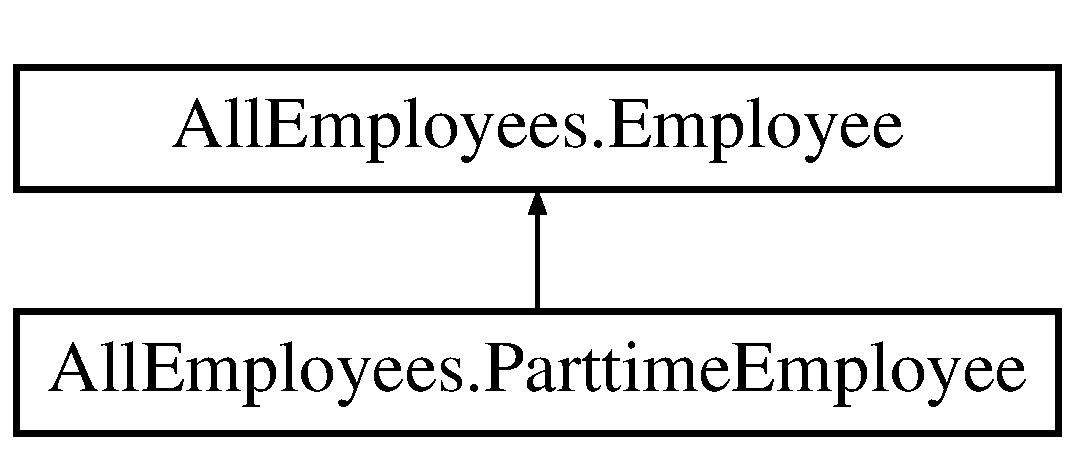
\includegraphics[height=2.000000cm]{class_all_employees_1_1_parttime_employee}
\end{center}
\end{figure}
\subsection*{Public Member Functions}
\begin{DoxyCompactItemize}
\item 
\hyperlink{class_all_employees_1_1_parttime_employee_aefdb20ed1cc9fb007068380a97e3f51e}{Parttime\+Employee} ()
\begin{DoxyCompactList}\small\item\em default constructor. Sets all values to default \end{DoxyCompactList}\item 
\hyperlink{class_all_employees_1_1_parttime_employee_a9c867461dd13baee1e84702999817ffb}{Parttime\+Employee} (string first\+Name, string last\+Name)
\begin{DoxyCompactList}\small\item\em overloaded constructor. Sets name to inputed names, set all other values to default \end{DoxyCompactList}\item 
\hyperlink{class_all_employees_1_1_parttime_employee_a4e465df9dcdecf0ba7eb89eae52d3f3a}{Parttime\+Employee} (string first\+Name, string last\+Name, int social\+Insurance\+Number, Date\+Time date\+Of\+Birth, Date\+Time date\+Of\+Hire, Date\+Time date\+Of\+Termination, float hourly\+Rate)
\begin{DoxyCompactList}\small\item\em overloaded constructor. Sets all values to the values given. no default values \end{DoxyCompactList}\item 
bool \hyperlink{class_all_employees_1_1_parttime_employee_ae9dfe4fa4f371c46c853cb499da663e7}{Validate} ()
\begin{DoxyCompactList}\small\item\em Used to determine in the object contains a valid employee. \end{DoxyCompactList}\item 
string \hyperlink{class_all_employees_1_1_parttime_employee_aab5cb221e05fda2cbac3d3ecb1398595}{Details} ()
\begin{DoxyCompactList}\small\item\em Used to print all employee data to the consol. \end{DoxyCompactList}\item 
override string \hyperlink{class_all_employees_1_1_parttime_employee_ab24493d33b967822f501bd92996a9e21}{To\+String} ()
\begin{DoxyCompactList}\small\item\em Overriden method To\+String used to return a formated string of all data. \end{DoxyCompactList}\item 
bool \hyperlink{class_all_employees_1_1_parttime_employee_a13b87ed00ebf4f834d6c9ff5b3051ca0}{Set\+Date\+Of\+Termination} (Date\+Time date)
\begin{DoxyCompactList}\small\item\em Setter for date\+Of\+Termination. \end{DoxyCompactList}\item 
bool \hyperlink{class_all_employees_1_1_parttime_employee_a305894433e372ba1511999889eebd7f0}{Set\+Date\+Of\+Termination} (string date)
\begin{DoxyCompactList}\small\item\em Setter for date\+Of\+Termination from string. \end{DoxyCompactList}\item 
bool \hyperlink{class_all_employees_1_1_parttime_employee_ad1738c15831d445694a56cf31eaf1e65}{Set\+Date\+Of\+Termination} (int year, int month, int day)
\begin{DoxyCompactList}\small\item\em Setter for date\+Of\+Termination from ints. \end{DoxyCompactList}\item 
bool \hyperlink{class_all_employees_1_1_parttime_employee_a13f02bfe441ed7b6f809f8ed5468bf7f}{Set\+Hourly\+Rate} (float rate)
\begin{DoxyCompactList}\small\item\em Setter for hourly\+Rate. \end{DoxyCompactList}\item 
bool \hyperlink{class_all_employees_1_1_parttime_employee_aa57cd09d4828cb5628f8b6200cdceeac}{Set\+Date\+Of\+Hire} (Date\+Time date)
\begin{DoxyCompactList}\small\item\em Setter for date\+Of\+Hire. \end{DoxyCompactList}\item 
bool \hyperlink{class_all_employees_1_1_parttime_employee_a7b1681699133e08b3c11900b73d757ef}{Set\+Date\+Of\+Hire} (string date)
\begin{DoxyCompactList}\small\item\em Setter for date\+Of\+Hire from string. \end{DoxyCompactList}\item 
bool \hyperlink{class_all_employees_1_1_parttime_employee_a8f49e4626627f95f098c56f092207a8e}{Set\+Date\+Of\+Hire} (int year, int month, int day)
\begin{DoxyCompactList}\small\item\em Setter for date\+Of\+Hire from ints. \end{DoxyCompactList}\item 
Date\+Time \hyperlink{class_all_employees_1_1_parttime_employee_a58fdbd9bf434cfeba1d3418bf1576100}{Get\+Date\+Of\+Termination} ()
\begin{DoxyCompactList}\small\item\em Getter for date\+Of\+Termination. \end{DoxyCompactList}\item 
string \hyperlink{class_all_employees_1_1_parttime_employee_aece6dee0304f86e5d03cb751bd3cbb49}{Get\+Date\+Of\+Termination\+String} ()
\begin{DoxyCompactList}\small\item\em Getter for date\+Of\+Termination that returns formatted string. \end{DoxyCompactList}\item 
float \hyperlink{class_all_employees_1_1_parttime_employee_a05b1fd21f7df07abc013ced6df7959f4}{Get\+Hourly\+Rate} ()
\begin{DoxyCompactList}\small\item\em Getter for hourly\+Rate. \end{DoxyCompactList}\item 
Date\+Time \hyperlink{class_all_employees_1_1_parttime_employee_a266fb09cc25fcf9d5e475d8859b1fdac}{Get\+Date\+Of\+Hire} ()
\begin{DoxyCompactList}\small\item\em Getter for date\+Of\+Hire. \end{DoxyCompactList}\item 
string \hyperlink{class_all_employees_1_1_parttime_employee_a18bd3a43e374b89bdd8f6e2ec9f9e51e}{Get\+Date\+Of\+Hire\+String} ()
\begin{DoxyCompactList}\small\item\em Getter for date\+Of\+Hire that returns formatted string. \end{DoxyCompactList}\end{DoxyCompactItemize}
\subsection*{Private Attributes}
\begin{DoxyCompactItemize}
\item 
\hypertarget{class_all_employees_1_1_parttime_employee_ae9217b6e9531dd5f6ac9029982bab405}{}Date\+Time {\bfseries date\+Of\+Hire}\label{class_all_employees_1_1_parttime_employee_ae9217b6e9531dd5f6ac9029982bab405}

\item 
\hypertarget{class_all_employees_1_1_parttime_employee_a98a60c754150cb7ff049b1a6f9eea5bc}{}Date\+Time {\bfseries date\+Of\+Termination}\label{class_all_employees_1_1_parttime_employee_a98a60c754150cb7ff049b1a6f9eea5bc}

\item 
\hypertarget{class_all_employees_1_1_parttime_employee_abbd98191b1a250e7910012c51f85bcea}{}float {\bfseries hourly\+Rate}\label{class_all_employees_1_1_parttime_employee_abbd98191b1a250e7910012c51f85bcea}

\end{DoxyCompactItemize}
\subsection*{Additional Inherited Members}


\subsection{Detailed Description}
{\bfseries Brief Description} The Parttime \hyperlink{class_all_employees_1_1_employee}{Employee} class is used to store and manage data about a employee who is hired for a part-\/time possition. This class is a child to \hyperlink{class_all_employees_1_1_employee}{Employee} class. It adds the date of hire and termination, and the employees hourly wage. If the constructor creates a invalid employee, a exception is thrown All other errors result in a defined return 

\begin{DoxyAuthor}{Author}
{\itshape Brandon} 
\end{DoxyAuthor}


\subsection{Constructor \& Destructor Documentation}
\hypertarget{class_all_employees_1_1_parttime_employee_aefdb20ed1cc9fb007068380a97e3f51e}{}\index{All\+Employees\+::\+Parttime\+Employee@{All\+Employees\+::\+Parttime\+Employee}!Parttime\+Employee@{Parttime\+Employee}}
\index{Parttime\+Employee@{Parttime\+Employee}!All\+Employees\+::\+Parttime\+Employee@{All\+Employees\+::\+Parttime\+Employee}}
\subsubsection[{Parttime\+Employee}]{\setlength{\rightskip}{0pt plus 5cm}All\+Employees.\+Parttime\+Employee.\+Parttime\+Employee (
\begin{DoxyParamCaption}
{}
\end{DoxyParamCaption}
)}\label{class_all_employees_1_1_parttime_employee_aefdb20ed1cc9fb007068380a97e3f51e}


default constructor. Sets all values to default 

{\bfseries Details}


\begin{DoxyParams}{Parameters}
{\em n/a} & \\
\hline
\end{DoxyParams}
\begin{DoxyReturn}{Returns}
n/a 
\end{DoxyReturn}
\hypertarget{class_all_employees_1_1_parttime_employee_a9c867461dd13baee1e84702999817ffb}{}\index{All\+Employees\+::\+Parttime\+Employee@{All\+Employees\+::\+Parttime\+Employee}!Parttime\+Employee@{Parttime\+Employee}}
\index{Parttime\+Employee@{Parttime\+Employee}!All\+Employees\+::\+Parttime\+Employee@{All\+Employees\+::\+Parttime\+Employee}}
\subsubsection[{Parttime\+Employee}]{\setlength{\rightskip}{0pt plus 5cm}All\+Employees.\+Parttime\+Employee.\+Parttime\+Employee (
\begin{DoxyParamCaption}
\item[{string}]{first\+Name, }
\item[{string}]{last\+Name}
\end{DoxyParamCaption}
)}\label{class_all_employees_1_1_parttime_employee_a9c867461dd13baee1e84702999817ffb}


overloaded constructor. Sets name to inputed names, set all other values to default 

{\bfseries Details}


\begin{DoxyParams}{Parameters}
{\em first\+Name} & -\/ {\bfseries string} -\/ First Name of employee to add to records \\
\hline
{\em last\+Name} & -\/ {\bfseries string} -\/ Last Name of employee to add to records\\
\hline
\end{DoxyParams}

\begin{DoxyExceptions}{Exceptions}
{\em $<$\+Failed\+Constructor\+Exception$>$} & -\/ If the constructor failed to create the object\\
\hline
\end{DoxyExceptions}
\begin{DoxyReturn}{Returns}
n/a 
\end{DoxyReturn}
\hypertarget{class_all_employees_1_1_parttime_employee_a4e465df9dcdecf0ba7eb89eae52d3f3a}{}\index{All\+Employees\+::\+Parttime\+Employee@{All\+Employees\+::\+Parttime\+Employee}!Parttime\+Employee@{Parttime\+Employee}}
\index{Parttime\+Employee@{Parttime\+Employee}!All\+Employees\+::\+Parttime\+Employee@{All\+Employees\+::\+Parttime\+Employee}}
\subsubsection[{Parttime\+Employee}]{\setlength{\rightskip}{0pt plus 5cm}All\+Employees.\+Parttime\+Employee.\+Parttime\+Employee (
\begin{DoxyParamCaption}
\item[{string}]{first\+Name, }
\item[{string}]{last\+Name, }
\item[{int}]{social\+Insurance\+Number, }
\item[{Date\+Time}]{date\+Of\+Birth, }
\item[{Date\+Time}]{date\+Of\+Hire, }
\item[{Date\+Time}]{date\+Of\+Termination, }
\item[{float}]{hourly\+Rate}
\end{DoxyParamCaption}
)}\label{class_all_employees_1_1_parttime_employee_a4e465df9dcdecf0ba7eb89eae52d3f3a}


overloaded constructor. Sets all values to the values given. no default values 

{\bfseries Details}


\begin{DoxyParams}{Parameters}
{\em first\+Name} & -\/ {\bfseries string} -\/ First Name of employee to add to records \\
\hline
{\em last\+Name} & -\/ {\bfseries string} -\/ Last Name of employee to add to records \\
\hline
{\em social\+Insurance\+Number} & -\/ {\bfseries int} -\/ Social Insurance Number of employee to add to records \\
\hline
{\em date\+Of\+Birth} & -\/ {\bfseries Date\+Time} -\/ Date Of Birth of employee to add to records \\
\hline
{\em date\+Of\+Hire} & -\/ {\bfseries Date\+Time} -\/ Date Of Hire of employee to add to records \\
\hline
{\em date\+Of\+Termination} & -\/ {\bfseries Date\+Time} -\/ Date Of Termination of employee to add to records \\
\hline
{\em hourly\+Rate} & -\/ {\bfseries float} -\/ Hourly Rate of employee to add to records\\
\hline
\end{DoxyParams}

\begin{DoxyExceptions}{Exceptions}
{\em $<$\+Failed\+Constructor\+Exception$>$} & -\/ If the constructor failed to create the object\\
\hline
\end{DoxyExceptions}
\begin{DoxyReturn}{Returns}
n/a 
\end{DoxyReturn}


\subsection{Member Function Documentation}
\hypertarget{class_all_employees_1_1_parttime_employee_aab5cb221e05fda2cbac3d3ecb1398595}{}\index{All\+Employees\+::\+Parttime\+Employee@{All\+Employees\+::\+Parttime\+Employee}!Details@{Details}}
\index{Details@{Details}!All\+Employees\+::\+Parttime\+Employee@{All\+Employees\+::\+Parttime\+Employee}}
\subsubsection[{Details}]{\setlength{\rightskip}{0pt plus 5cm}string All\+Employees.\+Parttime\+Employee.\+Details (
\begin{DoxyParamCaption}
{}
\end{DoxyParamCaption}
)}\label{class_all_employees_1_1_parttime_employee_aab5cb221e05fda2cbac3d3ecb1398595}


Used to print all employee data to the consol. 

{\bfseries Details}


\begin{DoxyParams}{Parameters}
{\em n/a} & \\
\hline
\end{DoxyParams}
\begin{DoxyReturn}{Returns}
user\+Info {\bfseries string} -\/ formatted string of employee data 
\end{DoxyReturn}
\hypertarget{class_all_employees_1_1_parttime_employee_a266fb09cc25fcf9d5e475d8859b1fdac}{}\index{All\+Employees\+::\+Parttime\+Employee@{All\+Employees\+::\+Parttime\+Employee}!Get\+Date\+Of\+Hire@{Get\+Date\+Of\+Hire}}
\index{Get\+Date\+Of\+Hire@{Get\+Date\+Of\+Hire}!All\+Employees\+::\+Parttime\+Employee@{All\+Employees\+::\+Parttime\+Employee}}
\subsubsection[{Get\+Date\+Of\+Hire}]{\setlength{\rightskip}{0pt plus 5cm}Date\+Time All\+Employees.\+Parttime\+Employee.\+Get\+Date\+Of\+Hire (
\begin{DoxyParamCaption}
{}
\end{DoxyParamCaption}
)}\label{class_all_employees_1_1_parttime_employee_a266fb09cc25fcf9d5e475d8859b1fdac}


Getter for date\+Of\+Hire. 

{\bfseries Details}


\begin{DoxyParams}{Parameters}
{\em n/a} & \\
\hline
\end{DoxyParams}
\begin{DoxyReturn}{Returns}
date\+Of\+Hire {\bfseries Date\+Time} 
\end{DoxyReturn}
\hypertarget{class_all_employees_1_1_parttime_employee_a18bd3a43e374b89bdd8f6e2ec9f9e51e}{}\index{All\+Employees\+::\+Parttime\+Employee@{All\+Employees\+::\+Parttime\+Employee}!Get\+Date\+Of\+Hire\+String@{Get\+Date\+Of\+Hire\+String}}
\index{Get\+Date\+Of\+Hire\+String@{Get\+Date\+Of\+Hire\+String}!All\+Employees\+::\+Parttime\+Employee@{All\+Employees\+::\+Parttime\+Employee}}
\subsubsection[{Get\+Date\+Of\+Hire\+String}]{\setlength{\rightskip}{0pt plus 5cm}string All\+Employees.\+Parttime\+Employee.\+Get\+Date\+Of\+Hire\+String (
\begin{DoxyParamCaption}
{}
\end{DoxyParamCaption}
)}\label{class_all_employees_1_1_parttime_employee_a18bd3a43e374b89bdd8f6e2ec9f9e51e}


Getter for date\+Of\+Hire that returns formatted string. 

{\bfseries Details}


\begin{DoxyParams}{Parameters}
{\em n/a} & \\
\hline
\end{DoxyParams}
\begin{DoxyReturn}{Returns}
date\+Of\+Hire {\bfseries string} 
\end{DoxyReturn}
\hypertarget{class_all_employees_1_1_parttime_employee_a58fdbd9bf434cfeba1d3418bf1576100}{}\index{All\+Employees\+::\+Parttime\+Employee@{All\+Employees\+::\+Parttime\+Employee}!Get\+Date\+Of\+Termination@{Get\+Date\+Of\+Termination}}
\index{Get\+Date\+Of\+Termination@{Get\+Date\+Of\+Termination}!All\+Employees\+::\+Parttime\+Employee@{All\+Employees\+::\+Parttime\+Employee}}
\subsubsection[{Get\+Date\+Of\+Termination}]{\setlength{\rightskip}{0pt plus 5cm}Date\+Time All\+Employees.\+Parttime\+Employee.\+Get\+Date\+Of\+Termination (
\begin{DoxyParamCaption}
{}
\end{DoxyParamCaption}
)}\label{class_all_employees_1_1_parttime_employee_a58fdbd9bf434cfeba1d3418bf1576100}


Getter for date\+Of\+Termination. 

{\bfseries Details}


\begin{DoxyParams}{Parameters}
{\em n/a} & \\
\hline
\end{DoxyParams}
\begin{DoxyReturn}{Returns}
date\+Of\+Termination {\bfseries Date\+Time} 
\end{DoxyReturn}
\hypertarget{class_all_employees_1_1_parttime_employee_aece6dee0304f86e5d03cb751bd3cbb49}{}\index{All\+Employees\+::\+Parttime\+Employee@{All\+Employees\+::\+Parttime\+Employee}!Get\+Date\+Of\+Termination\+String@{Get\+Date\+Of\+Termination\+String}}
\index{Get\+Date\+Of\+Termination\+String@{Get\+Date\+Of\+Termination\+String}!All\+Employees\+::\+Parttime\+Employee@{All\+Employees\+::\+Parttime\+Employee}}
\subsubsection[{Get\+Date\+Of\+Termination\+String}]{\setlength{\rightskip}{0pt plus 5cm}string All\+Employees.\+Parttime\+Employee.\+Get\+Date\+Of\+Termination\+String (
\begin{DoxyParamCaption}
{}
\end{DoxyParamCaption}
)}\label{class_all_employees_1_1_parttime_employee_aece6dee0304f86e5d03cb751bd3cbb49}


Getter for date\+Of\+Termination that returns formatted string. 

{\bfseries Details}


\begin{DoxyParams}{Parameters}
{\em n/a} & \\
\hline
\end{DoxyParams}
\begin{DoxyReturn}{Returns}
date\+Of\+Termination {\bfseries string} 
\end{DoxyReturn}
\hypertarget{class_all_employees_1_1_parttime_employee_a05b1fd21f7df07abc013ced6df7959f4}{}\index{All\+Employees\+::\+Parttime\+Employee@{All\+Employees\+::\+Parttime\+Employee}!Get\+Hourly\+Rate@{Get\+Hourly\+Rate}}
\index{Get\+Hourly\+Rate@{Get\+Hourly\+Rate}!All\+Employees\+::\+Parttime\+Employee@{All\+Employees\+::\+Parttime\+Employee}}
\subsubsection[{Get\+Hourly\+Rate}]{\setlength{\rightskip}{0pt plus 5cm}float All\+Employees.\+Parttime\+Employee.\+Get\+Hourly\+Rate (
\begin{DoxyParamCaption}
{}
\end{DoxyParamCaption}
)}\label{class_all_employees_1_1_parttime_employee_a05b1fd21f7df07abc013ced6df7959f4}


Getter for hourly\+Rate. 

{\bfseries Details}


\begin{DoxyParams}{Parameters}
{\em n/a} & \\
\hline
\end{DoxyParams}
\begin{DoxyReturn}{Returns}
hourly\+Rate {\bfseries float} 
\end{DoxyReturn}
\hypertarget{class_all_employees_1_1_parttime_employee_aa57cd09d4828cb5628f8b6200cdceeac}{}\index{All\+Employees\+::\+Parttime\+Employee@{All\+Employees\+::\+Parttime\+Employee}!Set\+Date\+Of\+Hire@{Set\+Date\+Of\+Hire}}
\index{Set\+Date\+Of\+Hire@{Set\+Date\+Of\+Hire}!All\+Employees\+::\+Parttime\+Employee@{All\+Employees\+::\+Parttime\+Employee}}
\subsubsection[{Set\+Date\+Of\+Hire}]{\setlength{\rightskip}{0pt plus 5cm}bool All\+Employees.\+Parttime\+Employee.\+Set\+Date\+Of\+Hire (
\begin{DoxyParamCaption}
\item[{Date\+Time}]{date}
\end{DoxyParamCaption}
)}\label{class_all_employees_1_1_parttime_employee_aa57cd09d4828cb5628f8b6200cdceeac}


Setter for date\+Of\+Hire. 

{\bfseries Details}


\begin{DoxyParams}{Parameters}
{\em date} & {\bfseries Date\+Time} -\/ The employees date of hire\\
\hline
\end{DoxyParams}
\begin{DoxyReturn}{Returns}
data\+Saved {\bfseries bool} -\/ true if input was valid and data was changed. False it data was not changed 
\end{DoxyReturn}
\hypertarget{class_all_employees_1_1_parttime_employee_a7b1681699133e08b3c11900b73d757ef}{}\index{All\+Employees\+::\+Parttime\+Employee@{All\+Employees\+::\+Parttime\+Employee}!Set\+Date\+Of\+Hire@{Set\+Date\+Of\+Hire}}
\index{Set\+Date\+Of\+Hire@{Set\+Date\+Of\+Hire}!All\+Employees\+::\+Parttime\+Employee@{All\+Employees\+::\+Parttime\+Employee}}
\subsubsection[{Set\+Date\+Of\+Hire}]{\setlength{\rightskip}{0pt plus 5cm}bool All\+Employees.\+Parttime\+Employee.\+Set\+Date\+Of\+Hire (
\begin{DoxyParamCaption}
\item[{string}]{date}
\end{DoxyParamCaption}
)}\label{class_all_employees_1_1_parttime_employee_a7b1681699133e08b3c11900b73d757ef}


Setter for date\+Of\+Hire from string. 

{\bfseries Details}


\begin{DoxyParams}{Parameters}
{\em date} & {\bfseries string} -\/ The employees date of hire\\
\hline
\end{DoxyParams}
\begin{DoxyReturn}{Returns}
data\+Saved {\bfseries bool} -\/ true if input was valid and data was changed. False it data was not changed 
\end{DoxyReturn}
\hypertarget{class_all_employees_1_1_parttime_employee_a8f49e4626627f95f098c56f092207a8e}{}\index{All\+Employees\+::\+Parttime\+Employee@{All\+Employees\+::\+Parttime\+Employee}!Set\+Date\+Of\+Hire@{Set\+Date\+Of\+Hire}}
\index{Set\+Date\+Of\+Hire@{Set\+Date\+Of\+Hire}!All\+Employees\+::\+Parttime\+Employee@{All\+Employees\+::\+Parttime\+Employee}}
\subsubsection[{Set\+Date\+Of\+Hire}]{\setlength{\rightskip}{0pt plus 5cm}bool All\+Employees.\+Parttime\+Employee.\+Set\+Date\+Of\+Hire (
\begin{DoxyParamCaption}
\item[{int}]{year, }
\item[{int}]{month, }
\item[{int}]{day}
\end{DoxyParamCaption}
)}\label{class_all_employees_1_1_parttime_employee_a8f49e4626627f95f098c56f092207a8e}


Setter for date\+Of\+Hire from ints. 

{\bfseries Details}


\begin{DoxyParams}{Parameters}
{\em year} & {\bfseries int} -\/ The year of the employees date\+Of\+Hire \\
\hline
{\em month} & {\bfseries int} -\/ The month of the employees date\+Of\+Hire \\
\hline
{\em day} & {\bfseries int} -\/ The day of the employees date\+Of\+Hire\\
\hline
\end{DoxyParams}
\begin{DoxyReturn}{Returns}
data\+Saved {\bfseries bool} -\/ true if input was valid and data was changed. False it data was not changed 
\end{DoxyReturn}
\hypertarget{class_all_employees_1_1_parttime_employee_a13b87ed00ebf4f834d6c9ff5b3051ca0}{}\index{All\+Employees\+::\+Parttime\+Employee@{All\+Employees\+::\+Parttime\+Employee}!Set\+Date\+Of\+Termination@{Set\+Date\+Of\+Termination}}
\index{Set\+Date\+Of\+Termination@{Set\+Date\+Of\+Termination}!All\+Employees\+::\+Parttime\+Employee@{All\+Employees\+::\+Parttime\+Employee}}
\subsubsection[{Set\+Date\+Of\+Termination}]{\setlength{\rightskip}{0pt plus 5cm}bool All\+Employees.\+Parttime\+Employee.\+Set\+Date\+Of\+Termination (
\begin{DoxyParamCaption}
\item[{Date\+Time}]{date}
\end{DoxyParamCaption}
)}\label{class_all_employees_1_1_parttime_employee_a13b87ed00ebf4f834d6c9ff5b3051ca0}


Setter for date\+Of\+Termination. 

{\bfseries Details}


\begin{DoxyParams}{Parameters}
{\em date} & {\bfseries Date\+Time} -\/ The employees date of termination\\
\hline
\end{DoxyParams}
\begin{DoxyReturn}{Returns}
data\+Saved {\bfseries bool} -\/ true if input was valid and data was changed. False it data was not changed 
\end{DoxyReturn}
\hypertarget{class_all_employees_1_1_parttime_employee_a305894433e372ba1511999889eebd7f0}{}\index{All\+Employees\+::\+Parttime\+Employee@{All\+Employees\+::\+Parttime\+Employee}!Set\+Date\+Of\+Termination@{Set\+Date\+Of\+Termination}}
\index{Set\+Date\+Of\+Termination@{Set\+Date\+Of\+Termination}!All\+Employees\+::\+Parttime\+Employee@{All\+Employees\+::\+Parttime\+Employee}}
\subsubsection[{Set\+Date\+Of\+Termination}]{\setlength{\rightskip}{0pt plus 5cm}bool All\+Employees.\+Parttime\+Employee.\+Set\+Date\+Of\+Termination (
\begin{DoxyParamCaption}
\item[{string}]{date}
\end{DoxyParamCaption}
)}\label{class_all_employees_1_1_parttime_employee_a305894433e372ba1511999889eebd7f0}


Setter for date\+Of\+Termination from string. 

{\bfseries Details}


\begin{DoxyParams}{Parameters}
{\em date} & {\bfseries string} -\/ The employees date of termination\\
\hline
\end{DoxyParams}
\begin{DoxyReturn}{Returns}
data\+Saved {\bfseries bool} -\/ true if input was valid and data was changed. False it data was not changed 
\end{DoxyReturn}
\hypertarget{class_all_employees_1_1_parttime_employee_ad1738c15831d445694a56cf31eaf1e65}{}\index{All\+Employees\+::\+Parttime\+Employee@{All\+Employees\+::\+Parttime\+Employee}!Set\+Date\+Of\+Termination@{Set\+Date\+Of\+Termination}}
\index{Set\+Date\+Of\+Termination@{Set\+Date\+Of\+Termination}!All\+Employees\+::\+Parttime\+Employee@{All\+Employees\+::\+Parttime\+Employee}}
\subsubsection[{Set\+Date\+Of\+Termination}]{\setlength{\rightskip}{0pt plus 5cm}bool All\+Employees.\+Parttime\+Employee.\+Set\+Date\+Of\+Termination (
\begin{DoxyParamCaption}
\item[{int}]{year, }
\item[{int}]{month, }
\item[{int}]{day}
\end{DoxyParamCaption}
)}\label{class_all_employees_1_1_parttime_employee_ad1738c15831d445694a56cf31eaf1e65}


Setter for date\+Of\+Termination from ints. 

{\bfseries Details}


\begin{DoxyParams}{Parameters}
{\em year} & {\bfseries int} -\/ The year of the employees Termination \\
\hline
{\em month} & {\bfseries int} -\/ The month of the employees Termination \\
\hline
{\em day} & {\bfseries int} -\/ The day of the employees Termination\\
\hline
\end{DoxyParams}
\begin{DoxyReturn}{Returns}
data\+Saved {\bfseries bool} -\/ true if input was valid and data was changed. False it data was not changed 
\end{DoxyReturn}
\hypertarget{class_all_employees_1_1_parttime_employee_a13f02bfe441ed7b6f809f8ed5468bf7f}{}\index{All\+Employees\+::\+Parttime\+Employee@{All\+Employees\+::\+Parttime\+Employee}!Set\+Hourly\+Rate@{Set\+Hourly\+Rate}}
\index{Set\+Hourly\+Rate@{Set\+Hourly\+Rate}!All\+Employees\+::\+Parttime\+Employee@{All\+Employees\+::\+Parttime\+Employee}}
\subsubsection[{Set\+Hourly\+Rate}]{\setlength{\rightskip}{0pt plus 5cm}bool All\+Employees.\+Parttime\+Employee.\+Set\+Hourly\+Rate (
\begin{DoxyParamCaption}
\item[{float}]{rate}
\end{DoxyParamCaption}
)}\label{class_all_employees_1_1_parttime_employee_a13f02bfe441ed7b6f809f8ed5468bf7f}


Setter for hourly\+Rate. 

{\bfseries Details}


\begin{DoxyParams}{Parameters}
{\em rate} & {\bfseries float} -\/ The employees hourly rate\\
\hline
\end{DoxyParams}
\begin{DoxyReturn}{Returns}
data\+Saved {\bfseries bool} -\/ true if input was valid and data was changed. False it data was not changed 
\end{DoxyReturn}
\hypertarget{class_all_employees_1_1_parttime_employee_ab24493d33b967822f501bd92996a9e21}{}\index{All\+Employees\+::\+Parttime\+Employee@{All\+Employees\+::\+Parttime\+Employee}!To\+String@{To\+String}}
\index{To\+String@{To\+String}!All\+Employees\+::\+Parttime\+Employee@{All\+Employees\+::\+Parttime\+Employee}}
\subsubsection[{To\+String}]{\setlength{\rightskip}{0pt plus 5cm}override string All\+Employees.\+Parttime\+Employee.\+To\+String (
\begin{DoxyParamCaption}
{}
\end{DoxyParamCaption}
)}\label{class_all_employees_1_1_parttime_employee_ab24493d33b967822f501bd92996a9e21}


Overriden method To\+String used to return a formated string of all data. 

{\bfseries Details}


\begin{DoxyParams}{Parameters}
{\em n/a} & \\
\hline
\end{DoxyParams}
\begin{DoxyReturn}{Returns}
employee\+String {\bfseries string} -\/ the formated string containing all employee data 
\end{DoxyReturn}
\hypertarget{class_all_employees_1_1_parttime_employee_ae9dfe4fa4f371c46c853cb499da663e7}{}\index{All\+Employees\+::\+Parttime\+Employee@{All\+Employees\+::\+Parttime\+Employee}!Validate@{Validate}}
\index{Validate@{Validate}!All\+Employees\+::\+Parttime\+Employee@{All\+Employees\+::\+Parttime\+Employee}}
\subsubsection[{Validate}]{\setlength{\rightskip}{0pt plus 5cm}bool All\+Employees.\+Parttime\+Employee.\+Validate (
\begin{DoxyParamCaption}
{}
\end{DoxyParamCaption}
)}\label{class_all_employees_1_1_parttime_employee_ae9dfe4fa4f371c46c853cb499da663e7}


Used to determine in the object contains a valid employee. 

{\bfseries Details}


\begin{DoxyParams}{Parameters}
{\em n/a} & \\
\hline
\end{DoxyParams}
\begin{DoxyReturn}{Returns}
data\+Valid -\/ {\bfseries bool} -\/ True if the object contains all data for a valid employee 
\end{DoxyReturn}


The documentation for this class was generated from the following file\+:\begin{DoxyCompactItemize}
\item 
C\+:/\+S\+E\+T\+Repo/trunk/\+E\+M\+S/trunk/\+All\+Employees/\+All\+Employees/Parttime\+Employee.\+cs\end{DoxyCompactItemize}

\hypertarget{class_my_all_employee_1_1_tests_1_1_parttime_employee_tests}{}\section{My\+All\+Employee.\+Tests.\+Parttime\+Employee\+Tests Class Reference}
\label{class_my_all_employee_1_1_tests_1_1_parttime_employee_tests}\index{My\+All\+Employee.\+Tests.\+Parttime\+Employee\+Tests@{My\+All\+Employee.\+Tests.\+Parttime\+Employee\+Tests}}


{\bfseries  Brief Description} This class is used to test the Parttime\+Employee methods in the All\+Employee class. The methods tested include the constructors, Details, Set\+Date\+Of\+Birth (all 3 overloaded methods), Set\+Dateof\+Hire (all 3 overloaded methods), Set\+Dateof\+Termination(all 3 overloaded methods), Set\+Hourly\+Rate and To\+String.  


\subsection*{Public Member Functions}
\begin{DoxyCompactItemize}
\item 
void \hyperlink{class_my_all_employee_1_1_tests_1_1_parttime_employee_tests_a8a3389bd51381be941170d33d311de77}{Constructor\+With\+Names\+Test\+Valid1} ()
\begin{DoxyCompactList}\small\item\em This unit test will check if either name contains anything other than a letter, apostrophe, dash. It will throw an exception if wrong. \end{DoxyCompactList}\item 
void \hyperlink{class_my_all_employee_1_1_tests_1_1_parttime_employee_tests_aacc90e48de93173876f79a4730249122}{Constructor\+With\+Names\+Test\+Valid2} ()
\begin{DoxyCompactList}\small\item\em This unit test will check if either name contains anything other than a letter, apostrophe, dash. It will throw an exception if wrong. \end{DoxyCompactList}\item 
void \hyperlink{class_my_all_employee_1_1_tests_1_1_parttime_employee_tests_a570acee022df6349ccb168fdd8795fb2}{Constructor\+With\+Names\+Test\+Valid3} ()
\begin{DoxyCompactList}\small\item\em This unit test will check if either name contains anything other than a letter, apostrophe, dash. It will throw an exception if wrong. \end{DoxyCompactList}\item 
void \hyperlink{class_my_all_employee_1_1_tests_1_1_parttime_employee_tests_a4bec66f82e4a17023d901772b4ba0ba2}{Constructor\+With\+Names\+Test\+Invalid\+Slash} ()
\begin{DoxyCompactList}\small\item\em This unit test will check if the constructor will fail and if the string is invalid because it contains a slash. \end{DoxyCompactList}\item 
void \hyperlink{class_my_all_employee_1_1_tests_1_1_parttime_employee_tests_a02d83e44f280d5e321da862bcde79145}{Constructor\+With\+Names\+Test\+Invalid\+Space} ()
\begin{DoxyCompactList}\small\item\em This unit test will check if the constructor will fail and if the string is invalid because it contains a space. \end{DoxyCompactList}\item 
void \hyperlink{class_my_all_employee_1_1_tests_1_1_parttime_employee_tests_afa5c9343c7245a45c6c39bc8c821d982}{Constructor\+With\+Names\+Test\+Invalid\+Number} ()
\begin{DoxyCompactList}\small\item\em This unit test will check if the constructor will fail and if the string is invalid because it contains a number. \end{DoxyCompactList}\item 
void \hyperlink{class_my_all_employee_1_1_tests_1_1_parttime_employee_tests_a0cbca99d6bc8eb60f9c2faa98f5441b9}{Constructor\+With\+All\+Param\+Test\+Valid1} ()
\begin{DoxyCompactList}\small\item\em This unit test will check the constructor that takes in all possible parameters, and give them all valid data. \end{DoxyCompactList}\item 
void \hyperlink{class_my_all_employee_1_1_tests_1_1_parttime_employee_tests_afc4d0c29429c2d4238d61c08c3fb2d3c}{Constructor\+With\+All\+Param\+Test\+Valid2} ()
\begin{DoxyCompactList}\small\item\em This unit test will check the constructor that takes in all possible parameters, and give them all valid data. \end{DoxyCompactList}\item 
void \hyperlink{class_my_all_employee_1_1_tests_1_1_parttime_employee_tests_a3ce1978ff98c7f208eaf239195bfab88}{Constructor\+With\+All\+Param\+Test\+Valid3} ()
\begin{DoxyCompactList}\small\item\em This unit test will check the constructor that takes in all possible parameters, and give them all valid data. \end{DoxyCompactList}\item 
void \hyperlink{class_my_all_employee_1_1_tests_1_1_parttime_employee_tests_a72a8ea8c0c900a8e045dabd5617ba707}{Constructor\+With\+All\+Param\+Test\+Invalid\+S\+I\+N} ()
\begin{DoxyCompactList}\small\item\em This unit test will check the constructor that takes in all possible parameters, and give them all invalid data. \end{DoxyCompactList}\item 
void \hyperlink{class_my_all_employee_1_1_tests_1_1_parttime_employee_tests_ae59654accc19b9d7e38ab7f4e0f34fb6}{Constructor\+With\+All\+Param\+Test\+Invalid\+D\+O\+H\+Before\+D\+O\+B} ()
\begin{DoxyCompactList}\small\item\em This unit test will check the constructor that takes in all possible parameters, and give them all invalid data. \end{DoxyCompactList}\item 
void \hyperlink{class_my_all_employee_1_1_tests_1_1_parttime_employee_tests_a36b5c50519f9866cab59de9204f00e91}{Constructor\+With\+All\+Param\+Test\+Invalid\+D\+O\+T\+Bofore\+D\+O\+H} ()
\begin{DoxyCompactList}\small\item\em This unit test will check the constructor that takes in all possible parameters, and give them all invalid data. \end{DoxyCompactList}\item 
void \hyperlink{class_my_all_employee_1_1_tests_1_1_parttime_employee_tests_acf0c1df829038c4ea3b2b4afd372bb48}{Constructor\+With\+All\+Param\+Test\+Invalid\+No\+D\+O\+H} ()
\begin{DoxyCompactList}\small\item\em This unit test will check the constructor that takes in all possible parameters, and give them all invalid data. \end{DoxyCompactList}\item 
void \hyperlink{class_my_all_employee_1_1_tests_1_1_parttime_employee_tests_a4c3a51bc9124ca9b76d227aa5a591e66}{Details\+Test\+Valid} ()
\begin{DoxyCompactList}\small\item\em This unit test will create an employee and runs it\textquotesingle{}s details, and will ensure that the string is what it should be(it is hardcoded) \end{DoxyCompactList}\item 
void \hyperlink{class_my_all_employee_1_1_tests_1_1_parttime_employee_tests_a93e1c4eaf3750132e8e60df585eb4be4}{To\+String\+Test\+Valid} ()
\begin{DoxyCompactList}\small\item\em This unit test will create an employee and runs it\textquotesingle{}s details, and will ensure that the string is what it should be(it is hardcoded) \end{DoxyCompactList}\item 
void \hyperlink{class_my_all_employee_1_1_tests_1_1_parttime_employee_tests_a0b68bd86c876d05b7823bdeaedef0112}{Set\+Date\+Of\+Hire\+Date\+Test\+Valid\+Date} ()
\begin{DoxyCompactList}\small\item\em This unit test will set the date of hire date to a valid date. \end{DoxyCompactList}\item 
void \hyperlink{class_my_all_employee_1_1_tests_1_1_parttime_employee_tests_aaca9d768d0e5b83ef1a74043417cd969}{Set\+Date\+Of\+Hire\+Date\+Test\+Invalid\+D\+O\+Hafter\+D\+O\+T} ()
\begin{DoxyCompactList}\small\item\em This unit test will set the date of hire date to an invalid date. \end{DoxyCompactList}\item 
void \hyperlink{class_my_all_employee_1_1_tests_1_1_parttime_employee_tests_ac5405b2d9ab9280666fcd50087abafb6}{Set\+Date\+Of\+Hire\+String\+Test\+Invalid\+D\+O\+Hbefore\+D\+O\+B} ()
\begin{DoxyCompactList}\small\item\em This unit test will set the date of hire string to an invalid string. \end{DoxyCompactList}\item 
void \hyperlink{class_my_all_employee_1_1_tests_1_1_parttime_employee_tests_a568d484fb9c0c9685e4520d6106253d7}{Set\+Date\+Of\+Hire\+String\+Test\+Valid\+String} ()
\begin{DoxyCompactList}\small\item\em This unit test will set the date of hire string to a valid string. \end{DoxyCompactList}\item 
void \hyperlink{class_my_all_employee_1_1_tests_1_1_parttime_employee_tests_aa0d53613837b28606160c2c147e6b909}{Set\+Date\+Of\+Hire\+String\+Test\+Invalid\+Format} ()
\begin{DoxyCompactList}\small\item\em This unit test will set the date of hire string to an invalid string. \end{DoxyCompactList}\item 
void \hyperlink{class_my_all_employee_1_1_tests_1_1_parttime_employee_tests_aadf36504af3cf262b6bb072f865d3802}{Set\+Date\+Of\+Hire\+String\+Test\+Invalid\+Date} ()
\begin{DoxyCompactList}\small\item\em This unit test will set the date of hire string to an invalid string. \end{DoxyCompactList}\item 
void \hyperlink{class_my_all_employee_1_1_tests_1_1_parttime_employee_tests_a162b58b62ab4c1107b68602b2f3a6bbc}{Set\+Date\+Of\+Hire\+String\+Test\+Invalid\+D\+O\+Hafter\+D\+O\+T} ()
\begin{DoxyCompactList}\small\item\em This unit test will set the date of hire string to an invalid string. \end{DoxyCompactList}\item 
void \hyperlink{class_my_all_employee_1_1_tests_1_1_parttime_employee_tests_add3e9cea0f3d03ba1b177590c697e0e1}{Set\+Date\+Of\+Hire\+Date\+Test\+Invalid\+D\+O\+Hbefore\+D\+O\+B} ()
\begin{DoxyCompactList}\small\item\em This unit test will set the date of hire date to an invalid date. \end{DoxyCompactList}\item 
void \hyperlink{class_my_all_employee_1_1_tests_1_1_parttime_employee_tests_a2662fee5c4dbd1e1d6d8038e42d1d615}{Set\+Date\+Of\+Hire\+Ints\+Test\+Invalid\+Letter} ()
\begin{DoxyCompactList}\small\item\em This unit test will set the date of hire date to an invalid date. \end{DoxyCompactList}\item 
void \hyperlink{class_my_all_employee_1_1_tests_1_1_parttime_employee_tests_a660a87661d1dea83cdbcdda435f9704c}{Set\+Date\+Of\+Hire\+Ints\+Test\+Valid} ()
\begin{DoxyCompactList}\small\item\em This unit test will set the date of hire date to a valid date. \end{DoxyCompactList}\item 
void \hyperlink{class_my_all_employee_1_1_tests_1_1_parttime_employee_tests_af43b5633da2c4a81340fdf02dafba5c0}{Set\+Date\+Of\+Hire\+Ints\+Test\+Invalid\+Date} ()
\begin{DoxyCompactList}\small\item\em This unit test will set the date of hire date to an invalid date. \end{DoxyCompactList}\item 
void \hyperlink{class_my_all_employee_1_1_tests_1_1_parttime_employee_tests_aaf42195f47a983540917b2e4a8ef2106}{Set\+Date\+Of\+Hire\+Ints\+Test\+Invalid\+D\+O\+Hafter\+D\+O\+T} ()
\begin{DoxyCompactList}\small\item\em This unit test will set the date of hire date to an invalid date. \end{DoxyCompactList}\item 
void \hyperlink{class_my_all_employee_1_1_tests_1_1_parttime_employee_tests_ac8c15a69d2b818c831a58bee0ad03015}{Set\+Date\+Of\+Hire\+Ints\+Test\+Invalid\+D\+O\+Hbefore\+D\+O\+B} ()
\begin{DoxyCompactList}\small\item\em This unit test will set the date of hire date to an invalid date. \end{DoxyCompactList}\item 
void \hyperlink{class_my_all_employee_1_1_tests_1_1_parttime_employee_tests_aa2ca527e770931b43f6353f68ed6b109}{Set\+Date\+Of\+Termination\+Date\+Test\+Valid\+Date} ()
\begin{DoxyCompactList}\small\item\em This unit test will set the date of termination date to a valid date. \end{DoxyCompactList}\item 
void \hyperlink{class_my_all_employee_1_1_tests_1_1_parttime_employee_tests_a25ab537e746d046721b346fedf0a7455}{Set\+Date\+Of\+Termination\+Date\+Test\+Invalid\+D\+O\+Tbefore\+D\+O\+H} ()
\begin{DoxyCompactList}\small\item\em This unit test will set the date of termination date to an invalid date. \end{DoxyCompactList}\item 
void \hyperlink{class_my_all_employee_1_1_tests_1_1_parttime_employee_tests_a3713ed1297ae952202955d529d4a4629}{Set\+Date\+Of\+Termination\+String\+Test\+Valid\+String} ()
\begin{DoxyCompactList}\small\item\em This unit test will set the date of termination string to a valid string. \end{DoxyCompactList}\item 
void \hyperlink{class_my_all_employee_1_1_tests_1_1_parttime_employee_tests_ad580c5170feee540d2cd2008e7c54a66}{Set\+Date\+Of\+Termination\+String\+Test\+Invalid\+Format} ()
\begin{DoxyCompactList}\small\item\em This unit test will set the date of termination string to an invalid string. \end{DoxyCompactList}\item 
void \hyperlink{class_my_all_employee_1_1_tests_1_1_parttime_employee_tests_a22bdea19ca3266a5e54c0792bf6b7ff7}{Set\+Date\+Of\+Termination\+String\+Test\+Invalid\+Date} ()
\begin{DoxyCompactList}\small\item\em This unit test will set the date of termination string to an invalid string. \end{DoxyCompactList}\item 
void \hyperlink{class_my_all_employee_1_1_tests_1_1_parttime_employee_tests_a73d08e15b8eb651bbc09e7aca26cd65f}{Set\+Date\+Of\+Termination\+String\+Test\+Invalid\+D\+O\+Tbefore\+D\+O\+H} ()
\begin{DoxyCompactList}\small\item\em This unit test will set the date of termination string to an invalid string. \end{DoxyCompactList}\item 
void \hyperlink{class_my_all_employee_1_1_tests_1_1_parttime_employee_tests_aa445325458236a1781eccd8ada0c9f17}{Set\+Date\+Of\+Termination\+Ints\+Test\+Invalid\+Letter} ()
\begin{DoxyCompactList}\small\item\em This unit test will set the date of termination string to an invalid string. \end{DoxyCompactList}\item 
void \hyperlink{class_my_all_employee_1_1_tests_1_1_parttime_employee_tests_aa47717f8a375b5bcfb637d87bcc62160}{Set\+Date\+Of\+Termination\+Ints\+Test\+Valid} ()
\begin{DoxyCompactList}\small\item\em This unit test will set the date of termination date to a valid date. \end{DoxyCompactList}\item 
void \hyperlink{class_my_all_employee_1_1_tests_1_1_parttime_employee_tests_a422a5225128e49d11e33ee3e4292f779}{Set\+Date\+Of\+Termination\+Ints\+Test\+Invalid\+Date} ()
\begin{DoxyCompactList}\small\item\em This unit test will set the date of termination date to an invalid date. \end{DoxyCompactList}\item 
void \hyperlink{class_my_all_employee_1_1_tests_1_1_parttime_employee_tests_a6b600dc38b952b9ada8e31bea5528d3d}{Set\+Date\+Of\+Termination\+Ints\+Test\+Invalid\+D\+O\+Tbefore\+D\+O\+H} ()
\begin{DoxyCompactList}\small\item\em This unit test will set the date of termination date to an invalid date. \end{DoxyCompactList}\item 
void \hyperlink{class_my_all_employee_1_1_tests_1_1_parttime_employee_tests_a1a74fc5a6b0121238e98a8f79b167946}{Set\+Hourly\+Rate\+Valid} ()
\begin{DoxyCompactList}\small\item\em This unit test will set the salary to a valid amount. \end{DoxyCompactList}\item 
void \hyperlink{class_my_all_employee_1_1_tests_1_1_parttime_employee_tests_a6f28346f0b36854cfc4f9b4d6e00da83}{Set\+Hourly\+Rate\+Invalid\+Negitive} ()
\begin{DoxyCompactList}\small\item\em This unit test will set the salary to an invalid amount. \end{DoxyCompactList}\end{DoxyCompactItemize}


\subsection{Detailed Description}
{\bfseries  Brief Description} This class is used to test the Parttime\+Employee methods in the All\+Employee class. The methods tested include the constructors, Details, Set\+Date\+Of\+Birth (all 3 overloaded methods), Set\+Dateof\+Hire (all 3 overloaded methods), Set\+Dateof\+Termination(all 3 overloaded methods), Set\+Hourly\+Rate and To\+String. 

\subsection{Member Function Documentation}
\hypertarget{class_my_all_employee_1_1_tests_1_1_parttime_employee_tests_ae59654accc19b9d7e38ab7f4e0f34fb6}{}\index{My\+All\+Employee\+::\+Tests\+::\+Parttime\+Employee\+Tests@{My\+All\+Employee\+::\+Tests\+::\+Parttime\+Employee\+Tests}!Constructor\+With\+All\+Param\+Test\+Invalid\+D\+O\+H\+Before\+D\+O\+B@{Constructor\+With\+All\+Param\+Test\+Invalid\+D\+O\+H\+Before\+D\+O\+B}}
\index{Constructor\+With\+All\+Param\+Test\+Invalid\+D\+O\+H\+Before\+D\+O\+B@{Constructor\+With\+All\+Param\+Test\+Invalid\+D\+O\+H\+Before\+D\+O\+B}!My\+All\+Employee\+::\+Tests\+::\+Parttime\+Employee\+Tests@{My\+All\+Employee\+::\+Tests\+::\+Parttime\+Employee\+Tests}}
\subsubsection[{Constructor\+With\+All\+Param\+Test\+Invalid\+D\+O\+H\+Before\+D\+O\+B}]{\setlength{\rightskip}{0pt plus 5cm}void My\+All\+Employee.\+Tests.\+Parttime\+Employee\+Tests.\+Constructor\+With\+All\+Param\+Test\+Invalid\+D\+O\+H\+Before\+D\+O\+B (
\begin{DoxyParamCaption}
{}
\end{DoxyParamCaption}
)}\label{class_my_all_employee_1_1_tests_1_1_parttime_employee_tests_ae59654accc19b9d7e38ab7f4e0f34fb6}


This unit test will check the constructor that takes in all possible parameters, and give them all invalid data. 

\textbackslash{} {\bfseries  Name of Method} \hyperlink{class_my_all_employee_1_1_tests_1_1_parttime_employee_tests_ae59654accc19b9d7e38ab7f4e0f34fb6}{Constructor\+With\+All\+Param\+Test\+Invalid\+D\+O\+H\+Before\+D\+O\+B()}

\textbackslash{} {\bfseries  How test is Conducted} This test is run automatically

\textbackslash{} {\bfseries  Type of Test} The type of test is an exception.

\textbackslash{} {\bfseries  Sample Data Sets} Date\+Time D\+O\+B = new Date\+Time(2003, 12, 12); Date\+Time D\+O\+H = new Date\+Time(2001, 02, 27); Date\+Time D\+O\+T = new Date\+Time(2006, 05, 21); \char`\"{}\+Brandon\char`\"{}, \char`\"{}\+Davies\char`\"{}, 123456789, D\+O\+B, D\+O\+H, D\+O\+T, 18

\textbackslash{} {\bfseries  Expected Result} The expected result is that there is an exception

\textbackslash{} {\bfseries  Actual Result} An exception is thrown \hypertarget{class_my_all_employee_1_1_tests_1_1_parttime_employee_tests_a36b5c50519f9866cab59de9204f00e91}{}\index{My\+All\+Employee\+::\+Tests\+::\+Parttime\+Employee\+Tests@{My\+All\+Employee\+::\+Tests\+::\+Parttime\+Employee\+Tests}!Constructor\+With\+All\+Param\+Test\+Invalid\+D\+O\+T\+Bofore\+D\+O\+H@{Constructor\+With\+All\+Param\+Test\+Invalid\+D\+O\+T\+Bofore\+D\+O\+H}}
\index{Constructor\+With\+All\+Param\+Test\+Invalid\+D\+O\+T\+Bofore\+D\+O\+H@{Constructor\+With\+All\+Param\+Test\+Invalid\+D\+O\+T\+Bofore\+D\+O\+H}!My\+All\+Employee\+::\+Tests\+::\+Parttime\+Employee\+Tests@{My\+All\+Employee\+::\+Tests\+::\+Parttime\+Employee\+Tests}}
\subsubsection[{Constructor\+With\+All\+Param\+Test\+Invalid\+D\+O\+T\+Bofore\+D\+O\+H}]{\setlength{\rightskip}{0pt plus 5cm}void My\+All\+Employee.\+Tests.\+Parttime\+Employee\+Tests.\+Constructor\+With\+All\+Param\+Test\+Invalid\+D\+O\+T\+Bofore\+D\+O\+H (
\begin{DoxyParamCaption}
{}
\end{DoxyParamCaption}
)}\label{class_my_all_employee_1_1_tests_1_1_parttime_employee_tests_a36b5c50519f9866cab59de9204f00e91}


This unit test will check the constructor that takes in all possible parameters, and give them all invalid data. 

\textbackslash{} {\bfseries  Name of Method} \hyperlink{class_my_all_employee_1_1_tests_1_1_parttime_employee_tests_a36b5c50519f9866cab59de9204f00e91}{Constructor\+With\+All\+Param\+Test\+Invalid\+D\+O\+T\+Bofore\+D\+O\+H()}

\textbackslash{} {\bfseries  How test is Conducted} This test is run automatically

\textbackslash{} {\bfseries  Type of Test} The type of test is an exception.

\textbackslash{} {\bfseries  Sample Data Sets} Date\+Time D\+O\+B = new Date\+Time(1993, 11, 14); Date\+Time D\+O\+H = new Date\+Time(2012, 10, 19); Date\+Time D\+O\+T = new Date\+Time(2010, 07, 29); \char`\"{}\+Brandon\char`\"{}, \char`\"{}\+Davies\char`\"{}, 123456789, D\+O\+B, D\+O\+H, D\+O\+T, 18

\textbackslash{} {\bfseries  Expected Result} The expected result is that there is an exception

\textbackslash{} {\bfseries  Actual Result} An exception is thrown \hypertarget{class_my_all_employee_1_1_tests_1_1_parttime_employee_tests_acf0c1df829038c4ea3b2b4afd372bb48}{}\index{My\+All\+Employee\+::\+Tests\+::\+Parttime\+Employee\+Tests@{My\+All\+Employee\+::\+Tests\+::\+Parttime\+Employee\+Tests}!Constructor\+With\+All\+Param\+Test\+Invalid\+No\+D\+O\+H@{Constructor\+With\+All\+Param\+Test\+Invalid\+No\+D\+O\+H}}
\index{Constructor\+With\+All\+Param\+Test\+Invalid\+No\+D\+O\+H@{Constructor\+With\+All\+Param\+Test\+Invalid\+No\+D\+O\+H}!My\+All\+Employee\+::\+Tests\+::\+Parttime\+Employee\+Tests@{My\+All\+Employee\+::\+Tests\+::\+Parttime\+Employee\+Tests}}
\subsubsection[{Constructor\+With\+All\+Param\+Test\+Invalid\+No\+D\+O\+H}]{\setlength{\rightskip}{0pt plus 5cm}void My\+All\+Employee.\+Tests.\+Parttime\+Employee\+Tests.\+Constructor\+With\+All\+Param\+Test\+Invalid\+No\+D\+O\+H (
\begin{DoxyParamCaption}
{}
\end{DoxyParamCaption}
)}\label{class_my_all_employee_1_1_tests_1_1_parttime_employee_tests_acf0c1df829038c4ea3b2b4afd372bb48}


This unit test will check the constructor that takes in all possible parameters, and give them all invalid data. 

\textbackslash{} {\bfseries  Name of Method} \hyperlink{class_my_all_employee_1_1_tests_1_1_parttime_employee_tests_acf0c1df829038c4ea3b2b4afd372bb48}{Constructor\+With\+All\+Param\+Test\+Invalid\+No\+D\+O\+H()}

\textbackslash{} {\bfseries  How test is Conducted} This test is run automatically

\textbackslash{} {\bfseries  Type of Test} The type of test is an exception.

\textbackslash{} {\bfseries  Sample Data Sets} Date\+Time D\+O\+B = new Date\+Time(1993, 11, 14); Date\+Time D\+O\+H = new Date\+Time(); Date\+Time D\+O\+T = new Date\+Time(); \char`\"{}\+Brandon\char`\"{}, \char`\"{}\+Davies\char`\"{}, 933456789, D\+O\+B, D\+O\+H, D\+O\+T, 180000

\textbackslash{} {\bfseries  Expected Result} The expected result is that there is an exception

\textbackslash{} {\bfseries  Actual Result} An exception is thrown \hypertarget{class_my_all_employee_1_1_tests_1_1_parttime_employee_tests_a72a8ea8c0c900a8e045dabd5617ba707}{}\index{My\+All\+Employee\+::\+Tests\+::\+Parttime\+Employee\+Tests@{My\+All\+Employee\+::\+Tests\+::\+Parttime\+Employee\+Tests}!Constructor\+With\+All\+Param\+Test\+Invalid\+S\+I\+N@{Constructor\+With\+All\+Param\+Test\+Invalid\+S\+I\+N}}
\index{Constructor\+With\+All\+Param\+Test\+Invalid\+S\+I\+N@{Constructor\+With\+All\+Param\+Test\+Invalid\+S\+I\+N}!My\+All\+Employee\+::\+Tests\+::\+Parttime\+Employee\+Tests@{My\+All\+Employee\+::\+Tests\+::\+Parttime\+Employee\+Tests}}
\subsubsection[{Constructor\+With\+All\+Param\+Test\+Invalid\+S\+I\+N}]{\setlength{\rightskip}{0pt plus 5cm}void My\+All\+Employee.\+Tests.\+Parttime\+Employee\+Tests.\+Constructor\+With\+All\+Param\+Test\+Invalid\+S\+I\+N (
\begin{DoxyParamCaption}
{}
\end{DoxyParamCaption}
)}\label{class_my_all_employee_1_1_tests_1_1_parttime_employee_tests_a72a8ea8c0c900a8e045dabd5617ba707}


This unit test will check the constructor that takes in all possible parameters, and give them all invalid data. 

\textbackslash{} {\bfseries  Name of Method} \hyperlink{class_my_all_employee_1_1_tests_1_1_parttime_employee_tests_a72a8ea8c0c900a8e045dabd5617ba707}{Constructor\+With\+All\+Param\+Test\+Invalid\+S\+I\+N()}

\textbackslash{} {\bfseries  How test is Conducted} This test is run automatically

\textbackslash{} {\bfseries  Type of Test} The type of test is an exception.

\textbackslash{} {\bfseries  Sample Data Sets} Date\+Time D\+O\+B = new Date\+Time(1984, 02, 15); Date\+Time D\+O\+H = new Date\+Time(1986, 20, 15); Date\+Time D\+O\+T = new Date\+Time(); \char`\"{}\+Brandon\char`\"{}, \char`\"{}\+Davies\char`\"{}, 1234756789, D\+O\+B, D\+O\+H, D\+O\+T, 18

\textbackslash{} {\bfseries  Expected Result} The expected result is that there is an exception

\textbackslash{} {\bfseries  Actual Result} An exception is thrown \hypertarget{class_my_all_employee_1_1_tests_1_1_parttime_employee_tests_a0cbca99d6bc8eb60f9c2faa98f5441b9}{}\index{My\+All\+Employee\+::\+Tests\+::\+Parttime\+Employee\+Tests@{My\+All\+Employee\+::\+Tests\+::\+Parttime\+Employee\+Tests}!Constructor\+With\+All\+Param\+Test\+Valid1@{Constructor\+With\+All\+Param\+Test\+Valid1}}
\index{Constructor\+With\+All\+Param\+Test\+Valid1@{Constructor\+With\+All\+Param\+Test\+Valid1}!My\+All\+Employee\+::\+Tests\+::\+Parttime\+Employee\+Tests@{My\+All\+Employee\+::\+Tests\+::\+Parttime\+Employee\+Tests}}
\subsubsection[{Constructor\+With\+All\+Param\+Test\+Valid1}]{\setlength{\rightskip}{0pt plus 5cm}void My\+All\+Employee.\+Tests.\+Parttime\+Employee\+Tests.\+Constructor\+With\+All\+Param\+Test\+Valid1 (
\begin{DoxyParamCaption}
{}
\end{DoxyParamCaption}
)}\label{class_my_all_employee_1_1_tests_1_1_parttime_employee_tests_a0cbca99d6bc8eb60f9c2faa98f5441b9}


This unit test will check the constructor that takes in all possible parameters, and give them all valid data. 

\textbackslash{} {\bfseries  Name of Method} \hyperlink{class_my_all_employee_1_1_tests_1_1_parttime_employee_tests_a0cbca99d6bc8eb60f9c2faa98f5441b9}{Constructor\+With\+All\+Param\+Test\+Valid1()}

\textbackslash{} {\bfseries  How test is Conducted} This test is run automatically

\textbackslash{} {\bfseries  Type of Test} The type of test is an normal/function.

\textbackslash{} {\bfseries  Sample Data Sets} Date\+Time D\+O\+B = new Date\+Time(1993, 04, 24); Date\+Time D\+O\+H = new Date\+Time(2000, 12, 12); Date\+Time D\+O\+T = new Date\+Time(); \char`\"{}\+Brandon\char`\"{}, \char`\"{}\+Davies\char`\"{}, 123456789, D\+O\+B, D\+O\+H, D\+O\+T, 18

\textbackslash{} {\bfseries  Expected Result} The expected result is that there is no exception

\textbackslash{} {\bfseries  Actual Result} An exception is not thrown \hypertarget{class_my_all_employee_1_1_tests_1_1_parttime_employee_tests_afc4d0c29429c2d4238d61c08c3fb2d3c}{}\index{My\+All\+Employee\+::\+Tests\+::\+Parttime\+Employee\+Tests@{My\+All\+Employee\+::\+Tests\+::\+Parttime\+Employee\+Tests}!Constructor\+With\+All\+Param\+Test\+Valid2@{Constructor\+With\+All\+Param\+Test\+Valid2}}
\index{Constructor\+With\+All\+Param\+Test\+Valid2@{Constructor\+With\+All\+Param\+Test\+Valid2}!My\+All\+Employee\+::\+Tests\+::\+Parttime\+Employee\+Tests@{My\+All\+Employee\+::\+Tests\+::\+Parttime\+Employee\+Tests}}
\subsubsection[{Constructor\+With\+All\+Param\+Test\+Valid2}]{\setlength{\rightskip}{0pt plus 5cm}void My\+All\+Employee.\+Tests.\+Parttime\+Employee\+Tests.\+Constructor\+With\+All\+Param\+Test\+Valid2 (
\begin{DoxyParamCaption}
{}
\end{DoxyParamCaption}
)}\label{class_my_all_employee_1_1_tests_1_1_parttime_employee_tests_afc4d0c29429c2d4238d61c08c3fb2d3c}


This unit test will check the constructor that takes in all possible parameters, and give them all valid data. 

\textbackslash{} {\bfseries  Name of Method} \hyperlink{class_my_all_employee_1_1_tests_1_1_parttime_employee_tests_afc4d0c29429c2d4238d61c08c3fb2d3c}{Constructor\+With\+All\+Param\+Test\+Valid2()}

\textbackslash{} {\bfseries  How test is Conducted} This test is run automatically

\textbackslash{} {\bfseries  Type of Test} The type of test is an normal/function.

\textbackslash{} {\bfseries  Sample Data Sets} Date\+Time D\+O\+B = new Date\+Time(1954, 08, 20); Date\+Time D\+O\+H = new Date\+Time(1994, 09, 03); Date\+Time D\+O\+T = new Date\+Time(2014, 12, 23); \char`\"{}\+Brandon\char`\"{}, \char`\"{}\+Mc\textquotesingle{}\+Davies\char`\"{}, 123456789, D\+O\+B, D\+O\+H, D\+O\+T, 18

\textbackslash{} {\bfseries  Expected Result} The expected result is that there is no exception

\textbackslash{} {\bfseries  Actual Result} An exception is not thrown \hypertarget{class_my_all_employee_1_1_tests_1_1_parttime_employee_tests_a3ce1978ff98c7f208eaf239195bfab88}{}\index{My\+All\+Employee\+::\+Tests\+::\+Parttime\+Employee\+Tests@{My\+All\+Employee\+::\+Tests\+::\+Parttime\+Employee\+Tests}!Constructor\+With\+All\+Param\+Test\+Valid3@{Constructor\+With\+All\+Param\+Test\+Valid3}}
\index{Constructor\+With\+All\+Param\+Test\+Valid3@{Constructor\+With\+All\+Param\+Test\+Valid3}!My\+All\+Employee\+::\+Tests\+::\+Parttime\+Employee\+Tests@{My\+All\+Employee\+::\+Tests\+::\+Parttime\+Employee\+Tests}}
\subsubsection[{Constructor\+With\+All\+Param\+Test\+Valid3}]{\setlength{\rightskip}{0pt plus 5cm}void My\+All\+Employee.\+Tests.\+Parttime\+Employee\+Tests.\+Constructor\+With\+All\+Param\+Test\+Valid3 (
\begin{DoxyParamCaption}
{}
\end{DoxyParamCaption}
)}\label{class_my_all_employee_1_1_tests_1_1_parttime_employee_tests_a3ce1978ff98c7f208eaf239195bfab88}


This unit test will check the constructor that takes in all possible parameters, and give them all valid data. 

\textbackslash{} {\bfseries  Name of Method} \hyperlink{class_my_all_employee_1_1_tests_1_1_parttime_employee_tests_a3ce1978ff98c7f208eaf239195bfab88}{Constructor\+With\+All\+Param\+Test\+Valid3()}

\textbackslash{} {\bfseries  How test is Conducted} This test is run automatically

\textbackslash{} {\bfseries  Type of Test} The type of test is an normal/function.

\textbackslash{} {\bfseries  Sample Data Sets} Date\+Time D\+O\+B = new Date\+Time(1830, 07, 29); Date\+Time D\+O\+H = new Date\+Time(2013, 05, 12); Date\+Time D\+O\+T = new Date\+Time(); \char`\"{}\+Brandon\char`\"{}, \char`\"{}\+Davies\char`\"{}, 123456789, D\+O\+B, D\+O\+H, D\+O\+T, 18

\textbackslash{} {\bfseries  Expected Result} The expected result is that there is no exception

\textbackslash{} {\bfseries  Actual Result} An exception is not thrown \hypertarget{class_my_all_employee_1_1_tests_1_1_parttime_employee_tests_afa5c9343c7245a45c6c39bc8c821d982}{}\index{My\+All\+Employee\+::\+Tests\+::\+Parttime\+Employee\+Tests@{My\+All\+Employee\+::\+Tests\+::\+Parttime\+Employee\+Tests}!Constructor\+With\+Names\+Test\+Invalid\+Number@{Constructor\+With\+Names\+Test\+Invalid\+Number}}
\index{Constructor\+With\+Names\+Test\+Invalid\+Number@{Constructor\+With\+Names\+Test\+Invalid\+Number}!My\+All\+Employee\+::\+Tests\+::\+Parttime\+Employee\+Tests@{My\+All\+Employee\+::\+Tests\+::\+Parttime\+Employee\+Tests}}
\subsubsection[{Constructor\+With\+Names\+Test\+Invalid\+Number}]{\setlength{\rightskip}{0pt plus 5cm}void My\+All\+Employee.\+Tests.\+Parttime\+Employee\+Tests.\+Constructor\+With\+Names\+Test\+Invalid\+Number (
\begin{DoxyParamCaption}
{}
\end{DoxyParamCaption}
)}\label{class_my_all_employee_1_1_tests_1_1_parttime_employee_tests_afa5c9343c7245a45c6c39bc8c821d982}


This unit test will check if the constructor will fail and if the string is invalid because it contains a number. 

\textbackslash{} {\bfseries  Name of Method} \hyperlink{class_my_all_employee_1_1_tests_1_1_parttime_employee_tests_afa5c9343c7245a45c6c39bc8c821d982}{Constructor\+With\+Names\+Test\+Invalid\+Number()}

\textbackslash{} {\bfseries  How test is Conducted} This test is run automatically

\textbackslash{} {\bfseries  Type of Test} The type of test is an exception.

\textbackslash{} {\bfseries  Sample Data Sets} \char`\"{}\+Brandon2\char`\"{}, \char`\"{}\+Davies\char`\"{}

\textbackslash{} {\bfseries  Expected Result} The expected result is that it will throw an exception

\textbackslash{} {\bfseries  Actual Result} An exception is thrown \hypertarget{class_my_all_employee_1_1_tests_1_1_parttime_employee_tests_a4bec66f82e4a17023d901772b4ba0ba2}{}\index{My\+All\+Employee\+::\+Tests\+::\+Parttime\+Employee\+Tests@{My\+All\+Employee\+::\+Tests\+::\+Parttime\+Employee\+Tests}!Constructor\+With\+Names\+Test\+Invalid\+Slash@{Constructor\+With\+Names\+Test\+Invalid\+Slash}}
\index{Constructor\+With\+Names\+Test\+Invalid\+Slash@{Constructor\+With\+Names\+Test\+Invalid\+Slash}!My\+All\+Employee\+::\+Tests\+::\+Parttime\+Employee\+Tests@{My\+All\+Employee\+::\+Tests\+::\+Parttime\+Employee\+Tests}}
\subsubsection[{Constructor\+With\+Names\+Test\+Invalid\+Slash}]{\setlength{\rightskip}{0pt plus 5cm}void My\+All\+Employee.\+Tests.\+Parttime\+Employee\+Tests.\+Constructor\+With\+Names\+Test\+Invalid\+Slash (
\begin{DoxyParamCaption}
{}
\end{DoxyParamCaption}
)}\label{class_my_all_employee_1_1_tests_1_1_parttime_employee_tests_a4bec66f82e4a17023d901772b4ba0ba2}


This unit test will check if the constructor will fail and if the string is invalid because it contains a slash. 

\textbackslash{} {\bfseries  Name of Method} \hyperlink{class_my_all_employee_1_1_tests_1_1_parttime_employee_tests_a4bec66f82e4a17023d901772b4ba0ba2}{Constructor\+With\+Names\+Test\+Invalid\+Slash()}

\textbackslash{} {\bfseries  How test is Conducted} This test is run automatically

\textbackslash{} {\bfseries  Type of Test} The type of test is an exception.

\textbackslash{} {\bfseries  Sample Data Sets} \char`\"{}\+Brandon\char`\"{}, \char`\"{}\+Mc/\+Davies\char`\"{}

\textbackslash{} {\bfseries  Expected Result} The expected result is that it will throw an exception

\textbackslash{} {\bfseries  Actual Result} An exception is thrown \hypertarget{class_my_all_employee_1_1_tests_1_1_parttime_employee_tests_a02d83e44f280d5e321da862bcde79145}{}\index{My\+All\+Employee\+::\+Tests\+::\+Parttime\+Employee\+Tests@{My\+All\+Employee\+::\+Tests\+::\+Parttime\+Employee\+Tests}!Constructor\+With\+Names\+Test\+Invalid\+Space@{Constructor\+With\+Names\+Test\+Invalid\+Space}}
\index{Constructor\+With\+Names\+Test\+Invalid\+Space@{Constructor\+With\+Names\+Test\+Invalid\+Space}!My\+All\+Employee\+::\+Tests\+::\+Parttime\+Employee\+Tests@{My\+All\+Employee\+::\+Tests\+::\+Parttime\+Employee\+Tests}}
\subsubsection[{Constructor\+With\+Names\+Test\+Invalid\+Space}]{\setlength{\rightskip}{0pt plus 5cm}void My\+All\+Employee.\+Tests.\+Parttime\+Employee\+Tests.\+Constructor\+With\+Names\+Test\+Invalid\+Space (
\begin{DoxyParamCaption}
{}
\end{DoxyParamCaption}
)}\label{class_my_all_employee_1_1_tests_1_1_parttime_employee_tests_a02d83e44f280d5e321da862bcde79145}


This unit test will check if the constructor will fail and if the string is invalid because it contains a space. 

\textbackslash{} {\bfseries  Name of Method} \hyperlink{class_my_all_employee_1_1_tests_1_1_parttime_employee_tests_a02d83e44f280d5e321da862bcde79145}{Constructor\+With\+Names\+Test\+Invalid\+Space()}

\textbackslash{} {\bfseries  How test is Conducted} This test is run automatically

\textbackslash{} {\bfseries  Type of Test} The type of test is an exception.

\textbackslash{} {\bfseries  Sample Data Sets} \char`\"{}\+Brandon\char`\"{}, \char`\"{}\+Mc Davies\char`\"{}

\textbackslash{} {\bfseries  Expected Result} The expected result is that it will throw an exception

\textbackslash{} {\bfseries  Actual Result} An exception is thrown \hypertarget{class_my_all_employee_1_1_tests_1_1_parttime_employee_tests_a8a3389bd51381be941170d33d311de77}{}\index{My\+All\+Employee\+::\+Tests\+::\+Parttime\+Employee\+Tests@{My\+All\+Employee\+::\+Tests\+::\+Parttime\+Employee\+Tests}!Constructor\+With\+Names\+Test\+Valid1@{Constructor\+With\+Names\+Test\+Valid1}}
\index{Constructor\+With\+Names\+Test\+Valid1@{Constructor\+With\+Names\+Test\+Valid1}!My\+All\+Employee\+::\+Tests\+::\+Parttime\+Employee\+Tests@{My\+All\+Employee\+::\+Tests\+::\+Parttime\+Employee\+Tests}}
\subsubsection[{Constructor\+With\+Names\+Test\+Valid1}]{\setlength{\rightskip}{0pt plus 5cm}void My\+All\+Employee.\+Tests.\+Parttime\+Employee\+Tests.\+Constructor\+With\+Names\+Test\+Valid1 (
\begin{DoxyParamCaption}
{}
\end{DoxyParamCaption}
)}\label{class_my_all_employee_1_1_tests_1_1_parttime_employee_tests_a8a3389bd51381be941170d33d311de77}


This unit test will check if either name contains anything other than a letter, apostrophe, dash. It will throw an exception if wrong. 

\textbackslash{} {\bfseries  Name of Method} \hyperlink{class_my_all_employee_1_1_tests_1_1_parttime_employee_tests_a8a3389bd51381be941170d33d311de77}{Constructor\+With\+Names\+Test\+Valid1()}

\textbackslash{} {\bfseries  How test is Conducted} This test is run automatically

\textbackslash{} {\bfseries  Type of Test} The type of test is normal/functional.

\textbackslash{} {\bfseries  Sample Data Sets} \char`\"{}\+Brandon\char`\"{}, \char`\"{}\+Davies\char`\"{}

\textbackslash{} {\bfseries  Expected Result} The expected result is that there is no exception

\textbackslash{} {\bfseries  Actual Result} There is no exception. \hypertarget{class_my_all_employee_1_1_tests_1_1_parttime_employee_tests_aacc90e48de93173876f79a4730249122}{}\index{My\+All\+Employee\+::\+Tests\+::\+Parttime\+Employee\+Tests@{My\+All\+Employee\+::\+Tests\+::\+Parttime\+Employee\+Tests}!Constructor\+With\+Names\+Test\+Valid2@{Constructor\+With\+Names\+Test\+Valid2}}
\index{Constructor\+With\+Names\+Test\+Valid2@{Constructor\+With\+Names\+Test\+Valid2}!My\+All\+Employee\+::\+Tests\+::\+Parttime\+Employee\+Tests@{My\+All\+Employee\+::\+Tests\+::\+Parttime\+Employee\+Tests}}
\subsubsection[{Constructor\+With\+Names\+Test\+Valid2}]{\setlength{\rightskip}{0pt plus 5cm}void My\+All\+Employee.\+Tests.\+Parttime\+Employee\+Tests.\+Constructor\+With\+Names\+Test\+Valid2 (
\begin{DoxyParamCaption}
{}
\end{DoxyParamCaption}
)}\label{class_my_all_employee_1_1_tests_1_1_parttime_employee_tests_aacc90e48de93173876f79a4730249122}


This unit test will check if either name contains anything other than a letter, apostrophe, dash. It will throw an exception if wrong. 

\textbackslash{} {\bfseries  Name of Method} \hyperlink{class_my_all_employee_1_1_tests_1_1_parttime_employee_tests_aacc90e48de93173876f79a4730249122}{Constructor\+With\+Names\+Test\+Valid2()}

\textbackslash{} {\bfseries  How test is Conducted} This test is run automatically

\textbackslash{} {\bfseries  Type of Test} The type of test is normal/functional.

\textbackslash{} {\bfseries  Sample Data Sets} \char`\"{}\+Brandon\char`\"{}, \char`\"{}\+Mc\textquotesingle{}\+Davies\char`\"{}

\textbackslash{} {\bfseries  Expected Result} The expected result is that there is no exception

\textbackslash{} {\bfseries  Actual Result} There is no exception. \hypertarget{class_my_all_employee_1_1_tests_1_1_parttime_employee_tests_a570acee022df6349ccb168fdd8795fb2}{}\index{My\+All\+Employee\+::\+Tests\+::\+Parttime\+Employee\+Tests@{My\+All\+Employee\+::\+Tests\+::\+Parttime\+Employee\+Tests}!Constructor\+With\+Names\+Test\+Valid3@{Constructor\+With\+Names\+Test\+Valid3}}
\index{Constructor\+With\+Names\+Test\+Valid3@{Constructor\+With\+Names\+Test\+Valid3}!My\+All\+Employee\+::\+Tests\+::\+Parttime\+Employee\+Tests@{My\+All\+Employee\+::\+Tests\+::\+Parttime\+Employee\+Tests}}
\subsubsection[{Constructor\+With\+Names\+Test\+Valid3}]{\setlength{\rightskip}{0pt plus 5cm}void My\+All\+Employee.\+Tests.\+Parttime\+Employee\+Tests.\+Constructor\+With\+Names\+Test\+Valid3 (
\begin{DoxyParamCaption}
{}
\end{DoxyParamCaption}
)}\label{class_my_all_employee_1_1_tests_1_1_parttime_employee_tests_a570acee022df6349ccb168fdd8795fb2}


This unit test will check if either name contains anything other than a letter, apostrophe, dash. It will throw an exception if wrong. 

\textbackslash{} {\bfseries  Name of Method} \hyperlink{class_my_all_employee_1_1_tests_1_1_parttime_employee_tests_a570acee022df6349ccb168fdd8795fb2}{Constructor\+With\+Names\+Test\+Valid3()}

\textbackslash{} {\bfseries  How test is Conducted} This test is run automatically

\textbackslash{} {\bfseries  Type of Test} The type of test is normal/functional.

\textbackslash{} {\bfseries  Sample Data Sets} \char`\"{}\+Brandon\char`\"{}, \char`\"{}\+Le\+Roy-\/\+Davies\char`\"{}

\textbackslash{} {\bfseries  Expected Result} The expected result is that there is no exception

\textbackslash{} {\bfseries  Actual Result} There is no exception. \hypertarget{class_my_all_employee_1_1_tests_1_1_parttime_employee_tests_a4c3a51bc9124ca9b76d227aa5a591e66}{}\index{My\+All\+Employee\+::\+Tests\+::\+Parttime\+Employee\+Tests@{My\+All\+Employee\+::\+Tests\+::\+Parttime\+Employee\+Tests}!Details\+Test\+Valid@{Details\+Test\+Valid}}
\index{Details\+Test\+Valid@{Details\+Test\+Valid}!My\+All\+Employee\+::\+Tests\+::\+Parttime\+Employee\+Tests@{My\+All\+Employee\+::\+Tests\+::\+Parttime\+Employee\+Tests}}
\subsubsection[{Details\+Test\+Valid}]{\setlength{\rightskip}{0pt plus 5cm}void My\+All\+Employee.\+Tests.\+Parttime\+Employee\+Tests.\+Details\+Test\+Valid (
\begin{DoxyParamCaption}
{}
\end{DoxyParamCaption}
)}\label{class_my_all_employee_1_1_tests_1_1_parttime_employee_tests_a4c3a51bc9124ca9b76d227aa5a591e66}


This unit test will create an employee and runs it\textquotesingle{}s details, and will ensure that the string is what it should be(it is hardcoded) 

\textbackslash{} {\bfseries  Name of Method} \hyperlink{class_my_all_employee_1_1_tests_1_1_parttime_employee_tests_a4c3a51bc9124ca9b76d227aa5a591e66}{Details\+Test\+Valid()}

\textbackslash{} {\bfseries  How test is Conducted} This test is run automatically

\textbackslash{} {\bfseries  Type of Test} The type of test is an normal/function.

\textbackslash{} {\bfseries  Sample Data Sets} Date\+Time D\+O\+B = new Date\+Time(1954, 08, 20); Date\+Time D\+O\+H = new Date\+Time(1994, 09, 03); Date\+Time D\+O\+T = new Date\+Time(2014, 12, 23); \char`\"{}\+Brandon\char`\"{}, \char`\"{}\+Davies\char`\"{}, 123456789, D\+O\+B, D\+O\+H, D\+O\+T, 18

\textbackslash{} {\bfseries  Expected Result} The expected result is that the string will be \char`\"{}\+Employee Type\+: Parttime\+Employee\textbackslash{}n\+Name\+: Brandon Davies\textbackslash{}n\+Social Insurance Number\+: 123 456 789\textbackslash{}n\+Date of Birth\+: 1954-\/08-\/20\textbackslash{}n\+Date of Hire\+: 1994-\/09-\/03\textbackslash{}n\+Date of Termionation2014-\/12-\/23\textbackslash{}n\+Hourly Rate\+: 18\char`\"{}

\textbackslash{} {\bfseries  Actual Result} The string is equivalent to \char`\"{}\+Employee Type\+: Parttime\+Employee\textbackslash{}n\+Name\+: Brandon Davies\textbackslash{}n\+Social Insurance Number\+: 123 456 789\textbackslash{}n\+Date of Birth\+: 1954-\/08-\/20\textbackslash{}n\+Date of Hire\+: 1994-\/09-\/03\textbackslash{}n\+Date of Termionation2014-\/12-\/23\textbackslash{}n\+Hourly Rate\+: 18\char`\"{} \hypertarget{class_my_all_employee_1_1_tests_1_1_parttime_employee_tests_aaca9d768d0e5b83ef1a74043417cd969}{}\index{My\+All\+Employee\+::\+Tests\+::\+Parttime\+Employee\+Tests@{My\+All\+Employee\+::\+Tests\+::\+Parttime\+Employee\+Tests}!Set\+Date\+Of\+Hire\+Date\+Test\+Invalid\+D\+O\+Hafter\+D\+O\+T@{Set\+Date\+Of\+Hire\+Date\+Test\+Invalid\+D\+O\+Hafter\+D\+O\+T}}
\index{Set\+Date\+Of\+Hire\+Date\+Test\+Invalid\+D\+O\+Hafter\+D\+O\+T@{Set\+Date\+Of\+Hire\+Date\+Test\+Invalid\+D\+O\+Hafter\+D\+O\+T}!My\+All\+Employee\+::\+Tests\+::\+Parttime\+Employee\+Tests@{My\+All\+Employee\+::\+Tests\+::\+Parttime\+Employee\+Tests}}
\subsubsection[{Set\+Date\+Of\+Hire\+Date\+Test\+Invalid\+D\+O\+Hafter\+D\+O\+T}]{\setlength{\rightskip}{0pt plus 5cm}void My\+All\+Employee.\+Tests.\+Parttime\+Employee\+Tests.\+Set\+Date\+Of\+Hire\+Date\+Test\+Invalid\+D\+O\+Hafter\+D\+O\+T (
\begin{DoxyParamCaption}
{}
\end{DoxyParamCaption}
)}\label{class_my_all_employee_1_1_tests_1_1_parttime_employee_tests_aaca9d768d0e5b83ef1a74043417cd969}


This unit test will set the date of hire date to an invalid date. 

\textbackslash{} {\bfseries  Name of Method} \hyperlink{class_my_all_employee_1_1_tests_1_1_parttime_employee_tests_aaca9d768d0e5b83ef1a74043417cd969}{Set\+Date\+Of\+Hire\+Date\+Test\+Invalid\+D\+O\+Hafter\+D\+O\+T()}

\textbackslash{} {\bfseries  How test is Conducted} This test is run automatically

\textbackslash{} {\bfseries  Type of Test} The type of test is an exception.

\textbackslash{} {\bfseries  Sample Data Sets} Date\+Time D\+O\+B = new Date\+Time(1954, 08, 20); Date\+Time D\+O\+H = new Date\+Time(1994, 09, 03); Date\+Time D\+O\+T = new Date\+Time(2000, 03, 23); \char`\"{}\+Brandon\char`\"{}, \char`\"{}\+Davies\char`\"{}, 123456789, D\+O\+B, D\+O\+H, D\+O\+T, 18 2012, 04, 23

\textbackslash{} {\bfseries  Expected Result} The expected result is the return value should be false and the data member should not have changed

\textbackslash{} {\bfseries  Actual Result} Return value is false, and the data member should not have changed \hypertarget{class_my_all_employee_1_1_tests_1_1_parttime_employee_tests_add3e9cea0f3d03ba1b177590c697e0e1}{}\index{My\+All\+Employee\+::\+Tests\+::\+Parttime\+Employee\+Tests@{My\+All\+Employee\+::\+Tests\+::\+Parttime\+Employee\+Tests}!Set\+Date\+Of\+Hire\+Date\+Test\+Invalid\+D\+O\+Hbefore\+D\+O\+B@{Set\+Date\+Of\+Hire\+Date\+Test\+Invalid\+D\+O\+Hbefore\+D\+O\+B}}
\index{Set\+Date\+Of\+Hire\+Date\+Test\+Invalid\+D\+O\+Hbefore\+D\+O\+B@{Set\+Date\+Of\+Hire\+Date\+Test\+Invalid\+D\+O\+Hbefore\+D\+O\+B}!My\+All\+Employee\+::\+Tests\+::\+Parttime\+Employee\+Tests@{My\+All\+Employee\+::\+Tests\+::\+Parttime\+Employee\+Tests}}
\subsubsection[{Set\+Date\+Of\+Hire\+Date\+Test\+Invalid\+D\+O\+Hbefore\+D\+O\+B}]{\setlength{\rightskip}{0pt plus 5cm}void My\+All\+Employee.\+Tests.\+Parttime\+Employee\+Tests.\+Set\+Date\+Of\+Hire\+Date\+Test\+Invalid\+D\+O\+Hbefore\+D\+O\+B (
\begin{DoxyParamCaption}
{}
\end{DoxyParamCaption}
)}\label{class_my_all_employee_1_1_tests_1_1_parttime_employee_tests_add3e9cea0f3d03ba1b177590c697e0e1}


This unit test will set the date of hire date to an invalid date. 

\textbackslash{} {\bfseries  Name of Method} \hyperlink{class_my_all_employee_1_1_tests_1_1_parttime_employee_tests_add3e9cea0f3d03ba1b177590c697e0e1}{Set\+Date\+Of\+Hire\+Date\+Test\+Invalid\+D\+O\+Hbefore\+D\+O\+B()}

\textbackslash{} {\bfseries  How test is Conducted} This test is run automatically

\textbackslash{} {\bfseries  Type of Test} The type of test is an exception.

\textbackslash{} {\bfseries  Sample Data Sets} Date\+Time(1954, 08, 20); Date\+Time(1994, 09, 03); Date\+Time(2000, 03, 23); \char`\"{}\+Brandon\char`\"{}, \char`\"{}\+Davies\char`\"{}, 123456789, D\+O\+B, D\+O\+H, D\+O\+T, 18 \char`\"{}1980-\/12-\/24\char`\"{}

\textbackslash{} {\bfseries  Expected Result} The expected result is the return value should be false and the data member should not have changed

\textbackslash{} {\bfseries  Actual Result} Return value is false, and the data member should not have changed \hypertarget{class_my_all_employee_1_1_tests_1_1_parttime_employee_tests_a0b68bd86c876d05b7823bdeaedef0112}{}\index{My\+All\+Employee\+::\+Tests\+::\+Parttime\+Employee\+Tests@{My\+All\+Employee\+::\+Tests\+::\+Parttime\+Employee\+Tests}!Set\+Date\+Of\+Hire\+Date\+Test\+Valid\+Date@{Set\+Date\+Of\+Hire\+Date\+Test\+Valid\+Date}}
\index{Set\+Date\+Of\+Hire\+Date\+Test\+Valid\+Date@{Set\+Date\+Of\+Hire\+Date\+Test\+Valid\+Date}!My\+All\+Employee\+::\+Tests\+::\+Parttime\+Employee\+Tests@{My\+All\+Employee\+::\+Tests\+::\+Parttime\+Employee\+Tests}}
\subsubsection[{Set\+Date\+Of\+Hire\+Date\+Test\+Valid\+Date}]{\setlength{\rightskip}{0pt plus 5cm}void My\+All\+Employee.\+Tests.\+Parttime\+Employee\+Tests.\+Set\+Date\+Of\+Hire\+Date\+Test\+Valid\+Date (
\begin{DoxyParamCaption}
{}
\end{DoxyParamCaption}
)}\label{class_my_all_employee_1_1_tests_1_1_parttime_employee_tests_a0b68bd86c876d05b7823bdeaedef0112}


This unit test will set the date of hire date to a valid date. 

\textbackslash{} {\bfseries  Name of Method} \hyperlink{class_my_all_employee_1_1_tests_1_1_parttime_employee_tests_a0b68bd86c876d05b7823bdeaedef0112}{Set\+Date\+Of\+Hire\+Date\+Test\+Valid\+Date()}

\textbackslash{} {\bfseries  How test is Conducted} This test is run automatically

\textbackslash{} {\bfseries  Type of Test} The type of test is an normal/function.

\textbackslash{} {\bfseries  Sample Data Sets} Date\+Time(2012, 04, 23)

\textbackslash{} {\bfseries  Expected Result} The expected result is the return value should be true and the data member should have changed

\textbackslash{} {\bfseries  Actual Result} Return value is true, and the data member should have changed \hypertarget{class_my_all_employee_1_1_tests_1_1_parttime_employee_tests_af43b5633da2c4a81340fdf02dafba5c0}{}\index{My\+All\+Employee\+::\+Tests\+::\+Parttime\+Employee\+Tests@{My\+All\+Employee\+::\+Tests\+::\+Parttime\+Employee\+Tests}!Set\+Date\+Of\+Hire\+Ints\+Test\+Invalid\+Date@{Set\+Date\+Of\+Hire\+Ints\+Test\+Invalid\+Date}}
\index{Set\+Date\+Of\+Hire\+Ints\+Test\+Invalid\+Date@{Set\+Date\+Of\+Hire\+Ints\+Test\+Invalid\+Date}!My\+All\+Employee\+::\+Tests\+::\+Parttime\+Employee\+Tests@{My\+All\+Employee\+::\+Tests\+::\+Parttime\+Employee\+Tests}}
\subsubsection[{Set\+Date\+Of\+Hire\+Ints\+Test\+Invalid\+Date}]{\setlength{\rightskip}{0pt plus 5cm}void My\+All\+Employee.\+Tests.\+Parttime\+Employee\+Tests.\+Set\+Date\+Of\+Hire\+Ints\+Test\+Invalid\+Date (
\begin{DoxyParamCaption}
{}
\end{DoxyParamCaption}
)}\label{class_my_all_employee_1_1_tests_1_1_parttime_employee_tests_af43b5633da2c4a81340fdf02dafba5c0}


This unit test will set the date of hire date to an invalid date. 

\textbackslash{} {\bfseries  Name of Method} \hyperlink{class_my_all_employee_1_1_tests_1_1_parttime_employee_tests_af43b5633da2c4a81340fdf02dafba5c0}{Set\+Date\+Of\+Hire\+Ints\+Test\+Invalid\+Date()}

\textbackslash{} {\bfseries  How test is Conducted} This test is run automatically

\textbackslash{} {\bfseries  Type of Test} The type of test is an exception.

\textbackslash{} {\bfseries  Sample Data Sets} 1993, 04, 31

\textbackslash{} {\bfseries  Expected Result} The expected result is the return value should be false and the data member should not have changed

\textbackslash{} {\bfseries  Actual Result} Return value is false, and the data member should not have changed \hypertarget{class_my_all_employee_1_1_tests_1_1_parttime_employee_tests_aaf42195f47a983540917b2e4a8ef2106}{}\index{My\+All\+Employee\+::\+Tests\+::\+Parttime\+Employee\+Tests@{My\+All\+Employee\+::\+Tests\+::\+Parttime\+Employee\+Tests}!Set\+Date\+Of\+Hire\+Ints\+Test\+Invalid\+D\+O\+Hafter\+D\+O\+T@{Set\+Date\+Of\+Hire\+Ints\+Test\+Invalid\+D\+O\+Hafter\+D\+O\+T}}
\index{Set\+Date\+Of\+Hire\+Ints\+Test\+Invalid\+D\+O\+Hafter\+D\+O\+T@{Set\+Date\+Of\+Hire\+Ints\+Test\+Invalid\+D\+O\+Hafter\+D\+O\+T}!My\+All\+Employee\+::\+Tests\+::\+Parttime\+Employee\+Tests@{My\+All\+Employee\+::\+Tests\+::\+Parttime\+Employee\+Tests}}
\subsubsection[{Set\+Date\+Of\+Hire\+Ints\+Test\+Invalid\+D\+O\+Hafter\+D\+O\+T}]{\setlength{\rightskip}{0pt plus 5cm}void My\+All\+Employee.\+Tests.\+Parttime\+Employee\+Tests.\+Set\+Date\+Of\+Hire\+Ints\+Test\+Invalid\+D\+O\+Hafter\+D\+O\+T (
\begin{DoxyParamCaption}
{}
\end{DoxyParamCaption}
)}\label{class_my_all_employee_1_1_tests_1_1_parttime_employee_tests_aaf42195f47a983540917b2e4a8ef2106}


This unit test will set the date of hire date to an invalid date. 

\textbackslash{} {\bfseries  Name of Method} \hyperlink{class_my_all_employee_1_1_tests_1_1_parttime_employee_tests_aaf42195f47a983540917b2e4a8ef2106}{Set\+Date\+Of\+Hire\+Ints\+Test\+Invalid\+D\+O\+Hafter\+D\+O\+T()}

\textbackslash{} {\bfseries  How test is Conducted} This test is run automatically

\textbackslash{} {\bfseries  Type of Test} The type of test is an exception.

\textbackslash{} {\bfseries  Sample Data Sets} Date\+Time(1954, 08, 20); Date\+Time(1994, 09, 03); Date\+Time(2000, 03, 23); \char`\"{}\+Brandon\char`\"{}, \char`\"{}\+Davies\char`\"{}, 123456789, D\+O\+B, D\+O\+H, D\+O\+T, 18 2001, 12, 24

\textbackslash{} {\bfseries  Expected Result} The expected result is the return value should be false and the data member should not have changed

\textbackslash{} {\bfseries  Actual Result} Return value is false, and the data member should not have changed \hypertarget{class_my_all_employee_1_1_tests_1_1_parttime_employee_tests_ac8c15a69d2b818c831a58bee0ad03015}{}\index{My\+All\+Employee\+::\+Tests\+::\+Parttime\+Employee\+Tests@{My\+All\+Employee\+::\+Tests\+::\+Parttime\+Employee\+Tests}!Set\+Date\+Of\+Hire\+Ints\+Test\+Invalid\+D\+O\+Hbefore\+D\+O\+B@{Set\+Date\+Of\+Hire\+Ints\+Test\+Invalid\+D\+O\+Hbefore\+D\+O\+B}}
\index{Set\+Date\+Of\+Hire\+Ints\+Test\+Invalid\+D\+O\+Hbefore\+D\+O\+B@{Set\+Date\+Of\+Hire\+Ints\+Test\+Invalid\+D\+O\+Hbefore\+D\+O\+B}!My\+All\+Employee\+::\+Tests\+::\+Parttime\+Employee\+Tests@{My\+All\+Employee\+::\+Tests\+::\+Parttime\+Employee\+Tests}}
\subsubsection[{Set\+Date\+Of\+Hire\+Ints\+Test\+Invalid\+D\+O\+Hbefore\+D\+O\+B}]{\setlength{\rightskip}{0pt plus 5cm}void My\+All\+Employee.\+Tests.\+Parttime\+Employee\+Tests.\+Set\+Date\+Of\+Hire\+Ints\+Test\+Invalid\+D\+O\+Hbefore\+D\+O\+B (
\begin{DoxyParamCaption}
{}
\end{DoxyParamCaption}
)}\label{class_my_all_employee_1_1_tests_1_1_parttime_employee_tests_ac8c15a69d2b818c831a58bee0ad03015}


This unit test will set the date of hire date to an invalid date. 

\textbackslash{} {\bfseries  Name of Method} \hyperlink{class_my_all_employee_1_1_tests_1_1_parttime_employee_tests_ac8c15a69d2b818c831a58bee0ad03015}{Set\+Date\+Of\+Hire\+Ints\+Test\+Invalid\+D\+O\+Hbefore\+D\+O\+B()}

\textbackslash{} {\bfseries  How test is Conducted} This test is run automatically

\textbackslash{} {\bfseries  Type of Test} The type of test is an exception.

\textbackslash{} {\bfseries  Sample Data Sets} Date\+Time(1984, 08, 20); Date\+Time(1994, 09, 03); Date\+Time(2000, 03, 23); \char`\"{}\+Brandon\char`\"{}, \char`\"{}\+Davies\char`\"{}, 123456789, D\+O\+B, D\+O\+H, D\+O\+T, 18 1980, 12, 24

\textbackslash{} {\bfseries  Expected Result} The expected result is the return value should be false and the data member should not have changed

\textbackslash{} {\bfseries  Actual Result} Return value is false, and the data member should not have changed \hypertarget{class_my_all_employee_1_1_tests_1_1_parttime_employee_tests_a2662fee5c4dbd1e1d6d8038e42d1d615}{}\index{My\+All\+Employee\+::\+Tests\+::\+Parttime\+Employee\+Tests@{My\+All\+Employee\+::\+Tests\+::\+Parttime\+Employee\+Tests}!Set\+Date\+Of\+Hire\+Ints\+Test\+Invalid\+Letter@{Set\+Date\+Of\+Hire\+Ints\+Test\+Invalid\+Letter}}
\index{Set\+Date\+Of\+Hire\+Ints\+Test\+Invalid\+Letter@{Set\+Date\+Of\+Hire\+Ints\+Test\+Invalid\+Letter}!My\+All\+Employee\+::\+Tests\+::\+Parttime\+Employee\+Tests@{My\+All\+Employee\+::\+Tests\+::\+Parttime\+Employee\+Tests}}
\subsubsection[{Set\+Date\+Of\+Hire\+Ints\+Test\+Invalid\+Letter}]{\setlength{\rightskip}{0pt plus 5cm}void My\+All\+Employee.\+Tests.\+Parttime\+Employee\+Tests.\+Set\+Date\+Of\+Hire\+Ints\+Test\+Invalid\+Letter (
\begin{DoxyParamCaption}
{}
\end{DoxyParamCaption}
)}\label{class_my_all_employee_1_1_tests_1_1_parttime_employee_tests_a2662fee5c4dbd1e1d6d8038e42d1d615}


This unit test will set the date of hire date to an invalid date. 

\textbackslash{} {\bfseries  Name of Method} \hyperlink{class_my_all_employee_1_1_tests_1_1_parttime_employee_tests_a2662fee5c4dbd1e1d6d8038e42d1d615}{Set\+Date\+Of\+Hire\+Ints\+Test\+Invalid\+Letter()}

\textbackslash{} {\bfseries  How test is Conducted} This test is run automatically

\textbackslash{} {\bfseries  Type of Test} The type of test is an exception.

\textbackslash{} {\bfseries  Sample Data Sets} \char`\"{}1993-\/s2-\/24\char`\"{}

\textbackslash{} {\bfseries  Expected Result} The expected result is the return value should be false and the data member should not have changed

\textbackslash{} {\bfseries  Actual Result} Return value is false, and the data member should not have changed \hypertarget{class_my_all_employee_1_1_tests_1_1_parttime_employee_tests_a660a87661d1dea83cdbcdda435f9704c}{}\index{My\+All\+Employee\+::\+Tests\+::\+Parttime\+Employee\+Tests@{My\+All\+Employee\+::\+Tests\+::\+Parttime\+Employee\+Tests}!Set\+Date\+Of\+Hire\+Ints\+Test\+Valid@{Set\+Date\+Of\+Hire\+Ints\+Test\+Valid}}
\index{Set\+Date\+Of\+Hire\+Ints\+Test\+Valid@{Set\+Date\+Of\+Hire\+Ints\+Test\+Valid}!My\+All\+Employee\+::\+Tests\+::\+Parttime\+Employee\+Tests@{My\+All\+Employee\+::\+Tests\+::\+Parttime\+Employee\+Tests}}
\subsubsection[{Set\+Date\+Of\+Hire\+Ints\+Test\+Valid}]{\setlength{\rightskip}{0pt plus 5cm}void My\+All\+Employee.\+Tests.\+Parttime\+Employee\+Tests.\+Set\+Date\+Of\+Hire\+Ints\+Test\+Valid (
\begin{DoxyParamCaption}
{}
\end{DoxyParamCaption}
)}\label{class_my_all_employee_1_1_tests_1_1_parttime_employee_tests_a660a87661d1dea83cdbcdda435f9704c}


This unit test will set the date of hire date to a valid date. 

\textbackslash{} {\bfseries  Name of Method} \hyperlink{class_my_all_employee_1_1_tests_1_1_parttime_employee_tests_a660a87661d1dea83cdbcdda435f9704c}{Set\+Date\+Of\+Hire\+Ints\+Test\+Valid()}

\textbackslash{} {\bfseries  How test is Conducted} This test is run automatically

\textbackslash{} {\bfseries  Type of Test} The type of test is an normal/function.

\textbackslash{} {\bfseries  Sample Data Sets} 1993, 04, 24

\textbackslash{} {\bfseries  Expected Result} The expected result is the return value should be true and the data member should have changed

\textbackslash{} {\bfseries  Actual Result} Return value is true, and the data member should have changed \hypertarget{class_my_all_employee_1_1_tests_1_1_parttime_employee_tests_aadf36504af3cf262b6bb072f865d3802}{}\index{My\+All\+Employee\+::\+Tests\+::\+Parttime\+Employee\+Tests@{My\+All\+Employee\+::\+Tests\+::\+Parttime\+Employee\+Tests}!Set\+Date\+Of\+Hire\+String\+Test\+Invalid\+Date@{Set\+Date\+Of\+Hire\+String\+Test\+Invalid\+Date}}
\index{Set\+Date\+Of\+Hire\+String\+Test\+Invalid\+Date@{Set\+Date\+Of\+Hire\+String\+Test\+Invalid\+Date}!My\+All\+Employee\+::\+Tests\+::\+Parttime\+Employee\+Tests@{My\+All\+Employee\+::\+Tests\+::\+Parttime\+Employee\+Tests}}
\subsubsection[{Set\+Date\+Of\+Hire\+String\+Test\+Invalid\+Date}]{\setlength{\rightskip}{0pt plus 5cm}void My\+All\+Employee.\+Tests.\+Parttime\+Employee\+Tests.\+Set\+Date\+Of\+Hire\+String\+Test\+Invalid\+Date (
\begin{DoxyParamCaption}
{}
\end{DoxyParamCaption}
)}\label{class_my_all_employee_1_1_tests_1_1_parttime_employee_tests_aadf36504af3cf262b6bb072f865d3802}


This unit test will set the date of hire string to an invalid string. 

\textbackslash{} {\bfseries  Name of Method} \hyperlink{class_my_all_employee_1_1_tests_1_1_parttime_employee_tests_aa0d53613837b28606160c2c147e6b909}{Set\+Date\+Of\+Hire\+String\+Test\+Invalid\+Format()}

\textbackslash{} {\bfseries  How test is Conducted} This test is run automatically

\textbackslash{} {\bfseries  Type of Test} The type of test is an exception.

\textbackslash{} {\bfseries  Sample Data Sets} \char`\"{}1993-\/13-\/24\char`\"{}

\textbackslash{} {\bfseries  Expected Result} The expected result is the return value should be false and the data member should not have changed

\textbackslash{} {\bfseries  Actual Result} Return value is false, and the data member should not have changed \hypertarget{class_my_all_employee_1_1_tests_1_1_parttime_employee_tests_a162b58b62ab4c1107b68602b2f3a6bbc}{}\index{My\+All\+Employee\+::\+Tests\+::\+Parttime\+Employee\+Tests@{My\+All\+Employee\+::\+Tests\+::\+Parttime\+Employee\+Tests}!Set\+Date\+Of\+Hire\+String\+Test\+Invalid\+D\+O\+Hafter\+D\+O\+T@{Set\+Date\+Of\+Hire\+String\+Test\+Invalid\+D\+O\+Hafter\+D\+O\+T}}
\index{Set\+Date\+Of\+Hire\+String\+Test\+Invalid\+D\+O\+Hafter\+D\+O\+T@{Set\+Date\+Of\+Hire\+String\+Test\+Invalid\+D\+O\+Hafter\+D\+O\+T}!My\+All\+Employee\+::\+Tests\+::\+Parttime\+Employee\+Tests@{My\+All\+Employee\+::\+Tests\+::\+Parttime\+Employee\+Tests}}
\subsubsection[{Set\+Date\+Of\+Hire\+String\+Test\+Invalid\+D\+O\+Hafter\+D\+O\+T}]{\setlength{\rightskip}{0pt plus 5cm}void My\+All\+Employee.\+Tests.\+Parttime\+Employee\+Tests.\+Set\+Date\+Of\+Hire\+String\+Test\+Invalid\+D\+O\+Hafter\+D\+O\+T (
\begin{DoxyParamCaption}
{}
\end{DoxyParamCaption}
)}\label{class_my_all_employee_1_1_tests_1_1_parttime_employee_tests_a162b58b62ab4c1107b68602b2f3a6bbc}


This unit test will set the date of hire string to an invalid string. 

\textbackslash{} {\bfseries  Name of Method} \hyperlink{class_my_all_employee_1_1_tests_1_1_parttime_employee_tests_a162b58b62ab4c1107b68602b2f3a6bbc}{Set\+Date\+Of\+Hire\+String\+Test\+Invalid\+D\+O\+Hafter\+D\+O\+T()}

\textbackslash{} {\bfseries  How test is Conducted} This test is run automatically

\textbackslash{} {\bfseries  Type of Test} The type of test is an exception.

\textbackslash{} {\bfseries  Sample Data Sets} Date\+Time(1954, 08, 20); Date\+Time(1994, 09, 03); Date\+Time(2000, 03, 23); \char`\"{}\+Brandon\char`\"{}, \char`\"{}\+Davies\char`\"{}, 123456789, D\+O\+B, D\+O\+H, D\+O\+T, 18 \char`\"{}2001-\/12-\/24\char`\"{}

\textbackslash{} {\bfseries  Expected Result} The expected result is the return value should be false and the data member should not have changed

\textbackslash{} {\bfseries  Actual Result} Return value is false, and the data member should not have changed \hypertarget{class_my_all_employee_1_1_tests_1_1_parttime_employee_tests_ac5405b2d9ab9280666fcd50087abafb6}{}\index{My\+All\+Employee\+::\+Tests\+::\+Parttime\+Employee\+Tests@{My\+All\+Employee\+::\+Tests\+::\+Parttime\+Employee\+Tests}!Set\+Date\+Of\+Hire\+String\+Test\+Invalid\+D\+O\+Hbefore\+D\+O\+B@{Set\+Date\+Of\+Hire\+String\+Test\+Invalid\+D\+O\+Hbefore\+D\+O\+B}}
\index{Set\+Date\+Of\+Hire\+String\+Test\+Invalid\+D\+O\+Hbefore\+D\+O\+B@{Set\+Date\+Of\+Hire\+String\+Test\+Invalid\+D\+O\+Hbefore\+D\+O\+B}!My\+All\+Employee\+::\+Tests\+::\+Parttime\+Employee\+Tests@{My\+All\+Employee\+::\+Tests\+::\+Parttime\+Employee\+Tests}}
\subsubsection[{Set\+Date\+Of\+Hire\+String\+Test\+Invalid\+D\+O\+Hbefore\+D\+O\+B}]{\setlength{\rightskip}{0pt plus 5cm}void My\+All\+Employee.\+Tests.\+Parttime\+Employee\+Tests.\+Set\+Date\+Of\+Hire\+String\+Test\+Invalid\+D\+O\+Hbefore\+D\+O\+B (
\begin{DoxyParamCaption}
{}
\end{DoxyParamCaption}
)}\label{class_my_all_employee_1_1_tests_1_1_parttime_employee_tests_ac5405b2d9ab9280666fcd50087abafb6}


This unit test will set the date of hire string to an invalid string. 

\textbackslash{} {\bfseries  Name of Method} \hyperlink{class_my_all_employee_1_1_tests_1_1_parttime_employee_tests_ac5405b2d9ab9280666fcd50087abafb6}{Set\+Date\+Of\+Hire\+String\+Test\+Invalid\+D\+O\+Hbefore\+D\+O\+B()}

\textbackslash{} {\bfseries  How test is Conducted} This test is run automatically

\textbackslash{} {\bfseries  Type of Test} The type of test is an exception.

\textbackslash{} {\bfseries  Sample Data Sets} Date\+Time D\+O\+B = new Date\+Time(1985, 08, 20); Date\+Time D\+O\+H = new Date\+Time(1994, 09, 03); Date\+Time D\+O\+T = new Date\+Time(2000, 03, 23); \char`\"{}\+Brandon\char`\"{}, \char`\"{}\+Davies\char`\"{}, 123456789, D\+O\+B, D\+O\+H, D\+O\+T, 18 1980, 04, 23

\textbackslash{} {\bfseries  Expected Result} The expected result is the return value should be false and the data member should not have changed

\textbackslash{} {\bfseries  Actual Result} Return value is false, and the data member should not have changed \hypertarget{class_my_all_employee_1_1_tests_1_1_parttime_employee_tests_aa0d53613837b28606160c2c147e6b909}{}\index{My\+All\+Employee\+::\+Tests\+::\+Parttime\+Employee\+Tests@{My\+All\+Employee\+::\+Tests\+::\+Parttime\+Employee\+Tests}!Set\+Date\+Of\+Hire\+String\+Test\+Invalid\+Format@{Set\+Date\+Of\+Hire\+String\+Test\+Invalid\+Format}}
\index{Set\+Date\+Of\+Hire\+String\+Test\+Invalid\+Format@{Set\+Date\+Of\+Hire\+String\+Test\+Invalid\+Format}!My\+All\+Employee\+::\+Tests\+::\+Parttime\+Employee\+Tests@{My\+All\+Employee\+::\+Tests\+::\+Parttime\+Employee\+Tests}}
\subsubsection[{Set\+Date\+Of\+Hire\+String\+Test\+Invalid\+Format}]{\setlength{\rightskip}{0pt plus 5cm}void My\+All\+Employee.\+Tests.\+Parttime\+Employee\+Tests.\+Set\+Date\+Of\+Hire\+String\+Test\+Invalid\+Format (
\begin{DoxyParamCaption}
{}
\end{DoxyParamCaption}
)}\label{class_my_all_employee_1_1_tests_1_1_parttime_employee_tests_aa0d53613837b28606160c2c147e6b909}


This unit test will set the date of hire string to an invalid string. 

\textbackslash{} {\bfseries  Name of Method} \hyperlink{class_my_all_employee_1_1_tests_1_1_parttime_employee_tests_aa0d53613837b28606160c2c147e6b909}{Set\+Date\+Of\+Hire\+String\+Test\+Invalid\+Format()}

\textbackslash{} {\bfseries  How test is Conducted} This test is run automatically

\textbackslash{} {\bfseries  Type of Test} The type of test is an exception.

\textbackslash{} {\bfseries  Sample Data Sets} \char`\"{}19930424\char`\"{}

\textbackslash{} {\bfseries  Expected Result} The expected result is the return value should be false and the data member should not have changed

\textbackslash{} {\bfseries  Actual Result} Return value is false, and the data member should not have changed \hypertarget{class_my_all_employee_1_1_tests_1_1_parttime_employee_tests_a568d484fb9c0c9685e4520d6106253d7}{}\index{My\+All\+Employee\+::\+Tests\+::\+Parttime\+Employee\+Tests@{My\+All\+Employee\+::\+Tests\+::\+Parttime\+Employee\+Tests}!Set\+Date\+Of\+Hire\+String\+Test\+Valid\+String@{Set\+Date\+Of\+Hire\+String\+Test\+Valid\+String}}
\index{Set\+Date\+Of\+Hire\+String\+Test\+Valid\+String@{Set\+Date\+Of\+Hire\+String\+Test\+Valid\+String}!My\+All\+Employee\+::\+Tests\+::\+Parttime\+Employee\+Tests@{My\+All\+Employee\+::\+Tests\+::\+Parttime\+Employee\+Tests}}
\subsubsection[{Set\+Date\+Of\+Hire\+String\+Test\+Valid\+String}]{\setlength{\rightskip}{0pt plus 5cm}void My\+All\+Employee.\+Tests.\+Parttime\+Employee\+Tests.\+Set\+Date\+Of\+Hire\+String\+Test\+Valid\+String (
\begin{DoxyParamCaption}
{}
\end{DoxyParamCaption}
)}\label{class_my_all_employee_1_1_tests_1_1_parttime_employee_tests_a568d484fb9c0c9685e4520d6106253d7}


This unit test will set the date of hire string to a valid string. 

\textbackslash{} {\bfseries  Name of Method} \hyperlink{class_my_all_employee_1_1_tests_1_1_parttime_employee_tests_a568d484fb9c0c9685e4520d6106253d7}{Set\+Date\+Of\+Hire\+String\+Test\+Valid\+String()}

\textbackslash{} {\bfseries  How test is Conducted} This test is run automatically

\textbackslash{} {\bfseries  Type of Test} The type of test is an normal/function.

\textbackslash{} {\bfseries  Sample Data Sets} \char`\"{}1993-\/04-\/24\char`\"{}

\textbackslash{} {\bfseries  Expected Result} The expected result is the return value should be true and the data member should have changed

\textbackslash{} {\bfseries  Actual Result} Return value is true, and the data member should have changed \hypertarget{class_my_all_employee_1_1_tests_1_1_parttime_employee_tests_a25ab537e746d046721b346fedf0a7455}{}\index{My\+All\+Employee\+::\+Tests\+::\+Parttime\+Employee\+Tests@{My\+All\+Employee\+::\+Tests\+::\+Parttime\+Employee\+Tests}!Set\+Date\+Of\+Termination\+Date\+Test\+Invalid\+D\+O\+Tbefore\+D\+O\+H@{Set\+Date\+Of\+Termination\+Date\+Test\+Invalid\+D\+O\+Tbefore\+D\+O\+H}}
\index{Set\+Date\+Of\+Termination\+Date\+Test\+Invalid\+D\+O\+Tbefore\+D\+O\+H@{Set\+Date\+Of\+Termination\+Date\+Test\+Invalid\+D\+O\+Tbefore\+D\+O\+H}!My\+All\+Employee\+::\+Tests\+::\+Parttime\+Employee\+Tests@{My\+All\+Employee\+::\+Tests\+::\+Parttime\+Employee\+Tests}}
\subsubsection[{Set\+Date\+Of\+Termination\+Date\+Test\+Invalid\+D\+O\+Tbefore\+D\+O\+H}]{\setlength{\rightskip}{0pt plus 5cm}void My\+All\+Employee.\+Tests.\+Parttime\+Employee\+Tests.\+Set\+Date\+Of\+Termination\+Date\+Test\+Invalid\+D\+O\+Tbefore\+D\+O\+H (
\begin{DoxyParamCaption}
{}
\end{DoxyParamCaption}
)}\label{class_my_all_employee_1_1_tests_1_1_parttime_employee_tests_a25ab537e746d046721b346fedf0a7455}


This unit test will set the date of termination date to an invalid date. 

\textbackslash{} {\bfseries  Name of Method} \hyperlink{class_my_all_employee_1_1_tests_1_1_parttime_employee_tests_a25ab537e746d046721b346fedf0a7455}{Set\+Date\+Of\+Termination\+Date\+Test\+Invalid\+D\+O\+Tbefore\+D\+O\+H()}

\textbackslash{} {\bfseries  How test is Conducted} This test is run automatically

\textbackslash{} {\bfseries  Type of Test} The type of test is an exception.

\textbackslash{} {\bfseries  Sample Data Sets} Date\+Time(1954, 08, 20); Date\+Time(1994, 09, 03); Date\+Time(2000, 03, 23); \char`\"{}\+Brandon\char`\"{}, \char`\"{}\+Davies\char`\"{}, 123456789, D\+O\+B, D\+O\+H, D\+O\+T, 18 1992, 04, 23

\textbackslash{} {\bfseries  Expected Result} The expected result is the return value should be false and the data member should not have changed

\textbackslash{} {\bfseries  Actual Result} Return value is false, and the data member should not have changed \hypertarget{class_my_all_employee_1_1_tests_1_1_parttime_employee_tests_aa2ca527e770931b43f6353f68ed6b109}{}\index{My\+All\+Employee\+::\+Tests\+::\+Parttime\+Employee\+Tests@{My\+All\+Employee\+::\+Tests\+::\+Parttime\+Employee\+Tests}!Set\+Date\+Of\+Termination\+Date\+Test\+Valid\+Date@{Set\+Date\+Of\+Termination\+Date\+Test\+Valid\+Date}}
\index{Set\+Date\+Of\+Termination\+Date\+Test\+Valid\+Date@{Set\+Date\+Of\+Termination\+Date\+Test\+Valid\+Date}!My\+All\+Employee\+::\+Tests\+::\+Parttime\+Employee\+Tests@{My\+All\+Employee\+::\+Tests\+::\+Parttime\+Employee\+Tests}}
\subsubsection[{Set\+Date\+Of\+Termination\+Date\+Test\+Valid\+Date}]{\setlength{\rightskip}{0pt plus 5cm}void My\+All\+Employee.\+Tests.\+Parttime\+Employee\+Tests.\+Set\+Date\+Of\+Termination\+Date\+Test\+Valid\+Date (
\begin{DoxyParamCaption}
{}
\end{DoxyParamCaption}
)}\label{class_my_all_employee_1_1_tests_1_1_parttime_employee_tests_aa2ca527e770931b43f6353f68ed6b109}


This unit test will set the date of termination date to a valid date. 

\textbackslash{} {\bfseries  Name of Method} \hyperlink{class_my_all_employee_1_1_tests_1_1_parttime_employee_tests_aa2ca527e770931b43f6353f68ed6b109}{Set\+Date\+Of\+Termination\+Date\+Test\+Valid\+Date()}

\textbackslash{} {\bfseries  How test is Conducted} This test is run automatically

\textbackslash{} {\bfseries  Type of Test} The type of test is an normal/function.

\textbackslash{} {\bfseries  Sample Data Sets} Date\+Time(1984, 08, 20); Date\+Time(1994, 09, 03); Date\+Time(2000, 03, 23); \char`\"{}\+Brandon\char`\"{}, \char`\"{}\+Davies\char`\"{}, 123456789, D\+O\+B, D\+O\+H, D\+O\+T, 18 2012, 04, 23

\textbackslash{} {\bfseries  Expected Result} The expected result is the return value should be true and the data member should have changed

\textbackslash{} {\bfseries  Actual Result} Return value is true, and the data member should have changed \hypertarget{class_my_all_employee_1_1_tests_1_1_parttime_employee_tests_a422a5225128e49d11e33ee3e4292f779}{}\index{My\+All\+Employee\+::\+Tests\+::\+Parttime\+Employee\+Tests@{My\+All\+Employee\+::\+Tests\+::\+Parttime\+Employee\+Tests}!Set\+Date\+Of\+Termination\+Ints\+Test\+Invalid\+Date@{Set\+Date\+Of\+Termination\+Ints\+Test\+Invalid\+Date}}
\index{Set\+Date\+Of\+Termination\+Ints\+Test\+Invalid\+Date@{Set\+Date\+Of\+Termination\+Ints\+Test\+Invalid\+Date}!My\+All\+Employee\+::\+Tests\+::\+Parttime\+Employee\+Tests@{My\+All\+Employee\+::\+Tests\+::\+Parttime\+Employee\+Tests}}
\subsubsection[{Set\+Date\+Of\+Termination\+Ints\+Test\+Invalid\+Date}]{\setlength{\rightskip}{0pt plus 5cm}void My\+All\+Employee.\+Tests.\+Parttime\+Employee\+Tests.\+Set\+Date\+Of\+Termination\+Ints\+Test\+Invalid\+Date (
\begin{DoxyParamCaption}
{}
\end{DoxyParamCaption}
)}\label{class_my_all_employee_1_1_tests_1_1_parttime_employee_tests_a422a5225128e49d11e33ee3e4292f779}


This unit test will set the date of termination date to an invalid date. 

\textbackslash{} {\bfseries  Name of Method} \hyperlink{class_my_all_employee_1_1_tests_1_1_parttime_employee_tests_a422a5225128e49d11e33ee3e4292f779}{Set\+Date\+Of\+Termination\+Ints\+Test\+Invalid\+Date()}

\textbackslash{} {\bfseries  How test is Conducted} This test is run automatically

\textbackslash{} {\bfseries  Type of Test} The type of test is an exception.

\textbackslash{} {\bfseries  Sample Data Sets} Date\+Time(1954, 08, 20); Date\+Time(1994, 09, 03); Date\+Time(2000, 03, 23); \char`\"{}\+Brandon\char`\"{}, \char`\"{}\+Davies\char`\"{}, 123456789, D\+O\+B, D\+O\+H, D\+O\+T, 18 1993, 04, 31

\textbackslash{} {\bfseries  Expected Result} The expected result is the return value should be false and the data member should not have changed

\textbackslash{} {\bfseries  Actual Result} Return value is false, and the data member should not have changed \hypertarget{class_my_all_employee_1_1_tests_1_1_parttime_employee_tests_a6b600dc38b952b9ada8e31bea5528d3d}{}\index{My\+All\+Employee\+::\+Tests\+::\+Parttime\+Employee\+Tests@{My\+All\+Employee\+::\+Tests\+::\+Parttime\+Employee\+Tests}!Set\+Date\+Of\+Termination\+Ints\+Test\+Invalid\+D\+O\+Tbefore\+D\+O\+H@{Set\+Date\+Of\+Termination\+Ints\+Test\+Invalid\+D\+O\+Tbefore\+D\+O\+H}}
\index{Set\+Date\+Of\+Termination\+Ints\+Test\+Invalid\+D\+O\+Tbefore\+D\+O\+H@{Set\+Date\+Of\+Termination\+Ints\+Test\+Invalid\+D\+O\+Tbefore\+D\+O\+H}!My\+All\+Employee\+::\+Tests\+::\+Parttime\+Employee\+Tests@{My\+All\+Employee\+::\+Tests\+::\+Parttime\+Employee\+Tests}}
\subsubsection[{Set\+Date\+Of\+Termination\+Ints\+Test\+Invalid\+D\+O\+Tbefore\+D\+O\+H}]{\setlength{\rightskip}{0pt plus 5cm}void My\+All\+Employee.\+Tests.\+Parttime\+Employee\+Tests.\+Set\+Date\+Of\+Termination\+Ints\+Test\+Invalid\+D\+O\+Tbefore\+D\+O\+H (
\begin{DoxyParamCaption}
{}
\end{DoxyParamCaption}
)}\label{class_my_all_employee_1_1_tests_1_1_parttime_employee_tests_a6b600dc38b952b9ada8e31bea5528d3d}


This unit test will set the date of termination date to an invalid date. 

\textbackslash{} {\bfseries  Name of Method} \hyperlink{class_my_all_employee_1_1_tests_1_1_parttime_employee_tests_a6b600dc38b952b9ada8e31bea5528d3d}{Set\+Date\+Of\+Termination\+Ints\+Test\+Invalid\+D\+O\+Tbefore\+D\+O\+H()}

\textbackslash{} {\bfseries  How test is Conducted} This test is run automatically

\textbackslash{} {\bfseries  Type of Test} The type of test is an exception.

\textbackslash{} {\bfseries  Sample Data Sets} Date\+Time(1954, 08, 20); Date\+Time(1994, 09, 03); Date\+Time(2000, 03, 23); \char`\"{}\+Brandon\char`\"{}, \char`\"{}\+Davies\char`\"{}, 123456789, D\+O\+B, D\+O\+H, D\+O\+T, 18 1991, 12, 24

\textbackslash{} {\bfseries  Expected Result} The expected result is the return value should be false and the data member should not have changed

\textbackslash{} {\bfseries  Actual Result} Return value is false, and the data member should not have changed \hypertarget{class_my_all_employee_1_1_tests_1_1_parttime_employee_tests_aa445325458236a1781eccd8ada0c9f17}{}\index{My\+All\+Employee\+::\+Tests\+::\+Parttime\+Employee\+Tests@{My\+All\+Employee\+::\+Tests\+::\+Parttime\+Employee\+Tests}!Set\+Date\+Of\+Termination\+Ints\+Test\+Invalid\+Letter@{Set\+Date\+Of\+Termination\+Ints\+Test\+Invalid\+Letter}}
\index{Set\+Date\+Of\+Termination\+Ints\+Test\+Invalid\+Letter@{Set\+Date\+Of\+Termination\+Ints\+Test\+Invalid\+Letter}!My\+All\+Employee\+::\+Tests\+::\+Parttime\+Employee\+Tests@{My\+All\+Employee\+::\+Tests\+::\+Parttime\+Employee\+Tests}}
\subsubsection[{Set\+Date\+Of\+Termination\+Ints\+Test\+Invalid\+Letter}]{\setlength{\rightskip}{0pt plus 5cm}void My\+All\+Employee.\+Tests.\+Parttime\+Employee\+Tests.\+Set\+Date\+Of\+Termination\+Ints\+Test\+Invalid\+Letter (
\begin{DoxyParamCaption}
{}
\end{DoxyParamCaption}
)}\label{class_my_all_employee_1_1_tests_1_1_parttime_employee_tests_aa445325458236a1781eccd8ada0c9f17}


This unit test will set the date of termination string to an invalid string. 

\textbackslash{} {\bfseries  Name of Method} \hyperlink{class_my_all_employee_1_1_tests_1_1_parttime_employee_tests_aa445325458236a1781eccd8ada0c9f17}{Set\+Date\+Of\+Termination\+Ints\+Test\+Invalid\+Letter()}

\textbackslash{} {\bfseries  How test is Conducted} This test is run automatically

\textbackslash{} {\bfseries  Type of Test} The type of test is an exception.

\textbackslash{} {\bfseries  Sample Data Sets} Date\+Time(1954, 08, 20); Date\+Time(1994, 09, 03); Date\+Time(2000, 03, 23); \char`\"{}\+Brandon\char`\"{}, \char`\"{}\+Davies\char`\"{}, 123456789, D\+O\+B, D\+O\+H, D\+O\+T, 18 \char`\"{}1993-\/s2-\/24\char`\"{}

\textbackslash{} {\bfseries  Expected Result} The expected result is the return value should be false and the data member should not have changed

\textbackslash{} {\bfseries  Actual Result} Return value is false, and the data member should not have changed \hypertarget{class_my_all_employee_1_1_tests_1_1_parttime_employee_tests_aa47717f8a375b5bcfb637d87bcc62160}{}\index{My\+All\+Employee\+::\+Tests\+::\+Parttime\+Employee\+Tests@{My\+All\+Employee\+::\+Tests\+::\+Parttime\+Employee\+Tests}!Set\+Date\+Of\+Termination\+Ints\+Test\+Valid@{Set\+Date\+Of\+Termination\+Ints\+Test\+Valid}}
\index{Set\+Date\+Of\+Termination\+Ints\+Test\+Valid@{Set\+Date\+Of\+Termination\+Ints\+Test\+Valid}!My\+All\+Employee\+::\+Tests\+::\+Parttime\+Employee\+Tests@{My\+All\+Employee\+::\+Tests\+::\+Parttime\+Employee\+Tests}}
\subsubsection[{Set\+Date\+Of\+Termination\+Ints\+Test\+Valid}]{\setlength{\rightskip}{0pt plus 5cm}void My\+All\+Employee.\+Tests.\+Parttime\+Employee\+Tests.\+Set\+Date\+Of\+Termination\+Ints\+Test\+Valid (
\begin{DoxyParamCaption}
{}
\end{DoxyParamCaption}
)}\label{class_my_all_employee_1_1_tests_1_1_parttime_employee_tests_aa47717f8a375b5bcfb637d87bcc62160}


This unit test will set the date of termination date to a valid date. 

\textbackslash{} {\bfseries  Name of Method} \hyperlink{class_my_all_employee_1_1_tests_1_1_parttime_employee_tests_aa47717f8a375b5bcfb637d87bcc62160}{Set\+Date\+Of\+Termination\+Ints\+Test\+Valid()}

\textbackslash{} {\bfseries  How test is Conducted} This test is run automatically

\textbackslash{} {\bfseries  Type of Test} The type of test is an normal/function.

\textbackslash{} {\bfseries  Sample Data Sets} Date\+Time(1954, 08, 20); Date\+Time(1994, 09, 03); Date\+Time(2000, 03, 23); \char`\"{}\+Brandon\char`\"{}, \char`\"{}\+Davies\char`\"{}, 123456789, D\+O\+B, D\+O\+H, D\+O\+T, 18 1997, 04, 24

\textbackslash{} {\bfseries  Expected Result} The expected result is the return value should be true and the data member should have changed

\textbackslash{} {\bfseries  Actual Result} Return value is true, and the data member should have changed \hypertarget{class_my_all_employee_1_1_tests_1_1_parttime_employee_tests_a22bdea19ca3266a5e54c0792bf6b7ff7}{}\index{My\+All\+Employee\+::\+Tests\+::\+Parttime\+Employee\+Tests@{My\+All\+Employee\+::\+Tests\+::\+Parttime\+Employee\+Tests}!Set\+Date\+Of\+Termination\+String\+Test\+Invalid\+Date@{Set\+Date\+Of\+Termination\+String\+Test\+Invalid\+Date}}
\index{Set\+Date\+Of\+Termination\+String\+Test\+Invalid\+Date@{Set\+Date\+Of\+Termination\+String\+Test\+Invalid\+Date}!My\+All\+Employee\+::\+Tests\+::\+Parttime\+Employee\+Tests@{My\+All\+Employee\+::\+Tests\+::\+Parttime\+Employee\+Tests}}
\subsubsection[{Set\+Date\+Of\+Termination\+String\+Test\+Invalid\+Date}]{\setlength{\rightskip}{0pt plus 5cm}void My\+All\+Employee.\+Tests.\+Parttime\+Employee\+Tests.\+Set\+Date\+Of\+Termination\+String\+Test\+Invalid\+Date (
\begin{DoxyParamCaption}
{}
\end{DoxyParamCaption}
)}\label{class_my_all_employee_1_1_tests_1_1_parttime_employee_tests_a22bdea19ca3266a5e54c0792bf6b7ff7}


This unit test will set the date of termination string to an invalid string. 

\textbackslash{} {\bfseries  Name of Method} \hyperlink{class_my_all_employee_1_1_tests_1_1_parttime_employee_tests_a22bdea19ca3266a5e54c0792bf6b7ff7}{Set\+Date\+Of\+Termination\+String\+Test\+Invalid\+Date()}

\textbackslash{} {\bfseries  How test is Conducted} This test is run automatically

\textbackslash{} {\bfseries  Type of Test} The type of test is an exception.

\textbackslash{} {\bfseries  Sample Data Sets} Date\+Time(1954, 08, 20); Date\+Time(1994, 09, 03); Date\+Time(2000, 03, 23); \char`\"{}\+Brandon\char`\"{}, \char`\"{}\+Davies\char`\"{}, 123456789, D\+O\+B, D\+O\+H, D\+O\+T, 18 \char`\"{}1997-\/13-\/24\char`\"{}

\textbackslash{} {\bfseries  Expected Result} The expected result is the return value should be false and the data member should not have changed

\textbackslash{} {\bfseries  Actual Result} Return value is false, and the data member should not have changed \hypertarget{class_my_all_employee_1_1_tests_1_1_parttime_employee_tests_a73d08e15b8eb651bbc09e7aca26cd65f}{}\index{My\+All\+Employee\+::\+Tests\+::\+Parttime\+Employee\+Tests@{My\+All\+Employee\+::\+Tests\+::\+Parttime\+Employee\+Tests}!Set\+Date\+Of\+Termination\+String\+Test\+Invalid\+D\+O\+Tbefore\+D\+O\+H@{Set\+Date\+Of\+Termination\+String\+Test\+Invalid\+D\+O\+Tbefore\+D\+O\+H}}
\index{Set\+Date\+Of\+Termination\+String\+Test\+Invalid\+D\+O\+Tbefore\+D\+O\+H@{Set\+Date\+Of\+Termination\+String\+Test\+Invalid\+D\+O\+Tbefore\+D\+O\+H}!My\+All\+Employee\+::\+Tests\+::\+Parttime\+Employee\+Tests@{My\+All\+Employee\+::\+Tests\+::\+Parttime\+Employee\+Tests}}
\subsubsection[{Set\+Date\+Of\+Termination\+String\+Test\+Invalid\+D\+O\+Tbefore\+D\+O\+H}]{\setlength{\rightskip}{0pt plus 5cm}void My\+All\+Employee.\+Tests.\+Parttime\+Employee\+Tests.\+Set\+Date\+Of\+Termination\+String\+Test\+Invalid\+D\+O\+Tbefore\+D\+O\+H (
\begin{DoxyParamCaption}
{}
\end{DoxyParamCaption}
)}\label{class_my_all_employee_1_1_tests_1_1_parttime_employee_tests_a73d08e15b8eb651bbc09e7aca26cd65f}


This unit test will set the date of termination string to an invalid string. 

\textbackslash{} {\bfseries  Name of Method} \hyperlink{class_my_all_employee_1_1_tests_1_1_parttime_employee_tests_a73d08e15b8eb651bbc09e7aca26cd65f}{Set\+Date\+Of\+Termination\+String\+Test\+Invalid\+D\+O\+Tbefore\+D\+O\+H()}

\textbackslash{} {\bfseries  How test is Conducted} This test is run automatically

\textbackslash{} {\bfseries  Type of Test} The type of test is an exception.

\textbackslash{} {\bfseries  Sample Data Sets} Date\+Time(1954, 08, 20); Date\+Time(1994, 09, 03); Date\+Time(2000, 03, 23); \char`\"{}\+Brandon\char`\"{}, \char`\"{}\+Davies\char`\"{}, 123456789, D\+O\+B, D\+O\+H, D\+O\+T, 18 \char`\"{}1993-\/12-\/24\char`\"{}

\textbackslash{} {\bfseries  Expected Result} The expected result is the return value should be false and the data member should not have changed

\textbackslash{} {\bfseries  Actual Result} Return value is false, and the data member should not have changed \hypertarget{class_my_all_employee_1_1_tests_1_1_parttime_employee_tests_ad580c5170feee540d2cd2008e7c54a66}{}\index{My\+All\+Employee\+::\+Tests\+::\+Parttime\+Employee\+Tests@{My\+All\+Employee\+::\+Tests\+::\+Parttime\+Employee\+Tests}!Set\+Date\+Of\+Termination\+String\+Test\+Invalid\+Format@{Set\+Date\+Of\+Termination\+String\+Test\+Invalid\+Format}}
\index{Set\+Date\+Of\+Termination\+String\+Test\+Invalid\+Format@{Set\+Date\+Of\+Termination\+String\+Test\+Invalid\+Format}!My\+All\+Employee\+::\+Tests\+::\+Parttime\+Employee\+Tests@{My\+All\+Employee\+::\+Tests\+::\+Parttime\+Employee\+Tests}}
\subsubsection[{Set\+Date\+Of\+Termination\+String\+Test\+Invalid\+Format}]{\setlength{\rightskip}{0pt plus 5cm}void My\+All\+Employee.\+Tests.\+Parttime\+Employee\+Tests.\+Set\+Date\+Of\+Termination\+String\+Test\+Invalid\+Format (
\begin{DoxyParamCaption}
{}
\end{DoxyParamCaption}
)}\label{class_my_all_employee_1_1_tests_1_1_parttime_employee_tests_ad580c5170feee540d2cd2008e7c54a66}


This unit test will set the date of termination string to an invalid string. 

\textbackslash{} {\bfseries  Name of Method} \hyperlink{class_my_all_employee_1_1_tests_1_1_parttime_employee_tests_ad580c5170feee540d2cd2008e7c54a66}{Set\+Date\+Of\+Termination\+String\+Test\+Invalid\+Format()}

\textbackslash{} {\bfseries  How test is Conducted} This test is run automatically

\textbackslash{} {\bfseries  Type of Test} The type of test is an exception.

\textbackslash{} {\bfseries  Sample Data Sets} Date\+Time(1954, 08, 20); Date\+Time(1994, 09, 03); Date\+Time(2000, 03, 23); \char`\"{}\+Brandon\char`\"{}, \char`\"{}\+Davies\char`\"{}, 123456789, D\+O\+B, D\+O\+H, D\+O\+T, 230000 \char`\"{}19970424\char`\"{}

\textbackslash{} {\bfseries  Expected Result} The expected result is the return value should be false and the data member should not have changed

\textbackslash{} {\bfseries  Actual Result} Return value is false, and the data member should not have changed \hypertarget{class_my_all_employee_1_1_tests_1_1_parttime_employee_tests_a3713ed1297ae952202955d529d4a4629}{}\index{My\+All\+Employee\+::\+Tests\+::\+Parttime\+Employee\+Tests@{My\+All\+Employee\+::\+Tests\+::\+Parttime\+Employee\+Tests}!Set\+Date\+Of\+Termination\+String\+Test\+Valid\+String@{Set\+Date\+Of\+Termination\+String\+Test\+Valid\+String}}
\index{Set\+Date\+Of\+Termination\+String\+Test\+Valid\+String@{Set\+Date\+Of\+Termination\+String\+Test\+Valid\+String}!My\+All\+Employee\+::\+Tests\+::\+Parttime\+Employee\+Tests@{My\+All\+Employee\+::\+Tests\+::\+Parttime\+Employee\+Tests}}
\subsubsection[{Set\+Date\+Of\+Termination\+String\+Test\+Valid\+String}]{\setlength{\rightskip}{0pt plus 5cm}void My\+All\+Employee.\+Tests.\+Parttime\+Employee\+Tests.\+Set\+Date\+Of\+Termination\+String\+Test\+Valid\+String (
\begin{DoxyParamCaption}
{}
\end{DoxyParamCaption}
)}\label{class_my_all_employee_1_1_tests_1_1_parttime_employee_tests_a3713ed1297ae952202955d529d4a4629}


This unit test will set the date of termination string to a valid string. 

\textbackslash{} {\bfseries  Name of Method} \hyperlink{class_my_all_employee_1_1_tests_1_1_parttime_employee_tests_a3713ed1297ae952202955d529d4a4629}{Set\+Date\+Of\+Termination\+String\+Test\+Valid\+String()}

\textbackslash{} {\bfseries  How test is Conducted} This test is run automatically

\textbackslash{} {\bfseries  Type of Test} The type of test is an normal/function.

\textbackslash{} {\bfseries  Sample Data Sets} Date\+Time(1954, 08, 20); Date\+Time(1994, 09, 03); Date\+Time(2000, 03, 23); \char`\"{}\+Brandon\char`\"{}, \char`\"{}\+Davies\char`\"{}, 123456789, D\+O\+B, D\+O\+H, D\+O\+T, 18 \char`\"{}1997-\/04-\/24\char`\"{}

\textbackslash{} {\bfseries  Expected Result} The expected result is the return value should be true and the data member should have changed

\textbackslash{} {\bfseries  Actual Result} Return value is true, and the data member should have changed \hypertarget{class_my_all_employee_1_1_tests_1_1_parttime_employee_tests_a6f28346f0b36854cfc4f9b4d6e00da83}{}\index{My\+All\+Employee\+::\+Tests\+::\+Parttime\+Employee\+Tests@{My\+All\+Employee\+::\+Tests\+::\+Parttime\+Employee\+Tests}!Set\+Hourly\+Rate\+Invalid\+Negitive@{Set\+Hourly\+Rate\+Invalid\+Negitive}}
\index{Set\+Hourly\+Rate\+Invalid\+Negitive@{Set\+Hourly\+Rate\+Invalid\+Negitive}!My\+All\+Employee\+::\+Tests\+::\+Parttime\+Employee\+Tests@{My\+All\+Employee\+::\+Tests\+::\+Parttime\+Employee\+Tests}}
\subsubsection[{Set\+Hourly\+Rate\+Invalid\+Negitive}]{\setlength{\rightskip}{0pt plus 5cm}void My\+All\+Employee.\+Tests.\+Parttime\+Employee\+Tests.\+Set\+Hourly\+Rate\+Invalid\+Negitive (
\begin{DoxyParamCaption}
{}
\end{DoxyParamCaption}
)}\label{class_my_all_employee_1_1_tests_1_1_parttime_employee_tests_a6f28346f0b36854cfc4f9b4d6e00da83}


This unit test will set the salary to an invalid amount. 

\textbackslash{} {\bfseries  Name of Method} \hyperlink{class_my_all_employee_1_1_tests_1_1_parttime_employee_tests_a6f28346f0b36854cfc4f9b4d6e00da83}{Set\+Hourly\+Rate\+Invalid\+Negitive()}

\textbackslash{} {\bfseries  How test is Conducted} This test is run automatically

\textbackslash{} {\bfseries  Type of Test} The type of test is an exception.

\textbackslash{} {\bfseries  Sample Data Sets} \char`\"{}\+Brandon\char`\"{}, \char`\"{}\+Davies\char`\"{} -\/18

\textbackslash{} {\bfseries  Expected Result} The expected result is the return value should be false and the data member should not have changed

\textbackslash{} {\bfseries  Actual Result} Return value is false, and the data member should not have changed \hypertarget{class_my_all_employee_1_1_tests_1_1_parttime_employee_tests_a1a74fc5a6b0121238e98a8f79b167946}{}\index{My\+All\+Employee\+::\+Tests\+::\+Parttime\+Employee\+Tests@{My\+All\+Employee\+::\+Tests\+::\+Parttime\+Employee\+Tests}!Set\+Hourly\+Rate\+Valid@{Set\+Hourly\+Rate\+Valid}}
\index{Set\+Hourly\+Rate\+Valid@{Set\+Hourly\+Rate\+Valid}!My\+All\+Employee\+::\+Tests\+::\+Parttime\+Employee\+Tests@{My\+All\+Employee\+::\+Tests\+::\+Parttime\+Employee\+Tests}}
\subsubsection[{Set\+Hourly\+Rate\+Valid}]{\setlength{\rightskip}{0pt plus 5cm}void My\+All\+Employee.\+Tests.\+Parttime\+Employee\+Tests.\+Set\+Hourly\+Rate\+Valid (
\begin{DoxyParamCaption}
{}
\end{DoxyParamCaption}
)}\label{class_my_all_employee_1_1_tests_1_1_parttime_employee_tests_a1a74fc5a6b0121238e98a8f79b167946}


This unit test will set the salary to a valid amount. 

\textbackslash{} {\bfseries  Name of Method} Set\+Hourly\+Rate()

\textbackslash{} {\bfseries  How test is Conducted} This test is run automatically

\textbackslash{} {\bfseries  Type of Test} The type of test is an normal/function.

\textbackslash{} {\bfseries  Sample Data Sets} \char`\"{}\+Brandon\char`\"{}, \char`\"{}\+Davies\char`\"{} 18

\textbackslash{} {\bfseries  Expected Result} The expected result is the return value should be true and the data member should have changed

\textbackslash{} {\bfseries  Actual Result} Return value is true, and the data member should have changed \hypertarget{class_my_all_employee_1_1_tests_1_1_parttime_employee_tests_a93e1c4eaf3750132e8e60df585eb4be4}{}\index{My\+All\+Employee\+::\+Tests\+::\+Parttime\+Employee\+Tests@{My\+All\+Employee\+::\+Tests\+::\+Parttime\+Employee\+Tests}!To\+String\+Test\+Valid@{To\+String\+Test\+Valid}}
\index{To\+String\+Test\+Valid@{To\+String\+Test\+Valid}!My\+All\+Employee\+::\+Tests\+::\+Parttime\+Employee\+Tests@{My\+All\+Employee\+::\+Tests\+::\+Parttime\+Employee\+Tests}}
\subsubsection[{To\+String\+Test\+Valid}]{\setlength{\rightskip}{0pt plus 5cm}void My\+All\+Employee.\+Tests.\+Parttime\+Employee\+Tests.\+To\+String\+Test\+Valid (
\begin{DoxyParamCaption}
{}
\end{DoxyParamCaption}
)}\label{class_my_all_employee_1_1_tests_1_1_parttime_employee_tests_a93e1c4eaf3750132e8e60df585eb4be4}


This unit test will create an employee and runs it\textquotesingle{}s details, and will ensure that the string is what it should be(it is hardcoded) 

\textbackslash{} {\bfseries  Name of Method} \hyperlink{class_my_all_employee_1_1_tests_1_1_parttime_employee_tests_a93e1c4eaf3750132e8e60df585eb4be4}{To\+String\+Test\+Valid()}

\textbackslash{} {\bfseries  How test is Conducted} This test is run automatically

\textbackslash{} {\bfseries  Type of Test} The type of test is an normal/function.

\textbackslash{} {\bfseries  Sample Data Sets} Date\+Time D\+O\+B = new Date\+Time(1954, 08, 20); Date\+Time D\+O\+H = new Date\+Time(1994, 09, 03); Date\+Time D\+O\+T = new Date\+Time(2014, 12, 23); \char`\"{}\+Brandon\char`\"{}, \char`\"{}\+Davies\char`\"{}, 123456789, D\+O\+B, D\+O\+H, D\+O\+T, 18

\textbackslash{} {\bfseries  Expected Result} The expected result is that the string will be \char`\"{}$\vert$\+P\+T$\vert$\+Brandon$\vert$\+Davies$\vert$123456789$\vert$1954-\/08-\/20$\vert$1994-\/09-\/03$\vert$2014-\/12-\/23$\vert$18$\vert$\char`\"{}

\textbackslash{} {\bfseries  Actual Result} The string is equivalent to \char`\"{}$\vert$\+P\+T$\vert$\+Brandon$\vert$\+Davies$\vert$123456789$\vert$1954-\/08-\/20$\vert$1994-\/09-\/03$\vert$2014-\/12-\/23$\vert$18$\vert$\char`\"{} 

The documentation for this class was generated from the following file\+:\begin{DoxyCompactItemize}
\item 
C\+:/\+S\+E\+T\+Repo/trunk/\+E\+M\+S/trunk/\+All\+Employees/\+My\+All\+Employee.\+Tests/Part\+Time\+Employee\+Tests.\+cs\end{DoxyCompactItemize}

\hypertarget{class_e_m_s___run_line_1_1_program}{}\section{E\+M\+S\+\_\+\+Run\+Line.\+Program Class Reference}
\label{class_e_m_s___run_line_1_1_program}\index{E\+M\+S\+\_\+\+Run\+Line.\+Program@{E\+M\+S\+\_\+\+Run\+Line.\+Program}}
\subsection*{Static Private Member Functions}
\begin{DoxyCompactItemize}
\item 
\hypertarget{class_e_m_s___run_line_1_1_program_a9468a48e40f12fcca1ab0b4e02dbf978}{}static void {\bfseries Main} (string\mbox{[}$\,$\mbox{]} args)\label{class_e_m_s___run_line_1_1_program_a9468a48e40f12fcca1ab0b4e02dbf978}

\end{DoxyCompactItemize}


The documentation for this class was generated from the following file\+:\begin{DoxyCompactItemize}
\item 
C\+:/\+S\+E\+T\+Repo/trunk/\+E\+M\+S/trunk/\+E\+M\+S-\/\+Run\+Line/\+E\+M\+S-\/\+Run\+Line/Program.\+cs\end{DoxyCompactItemize}

\hypertarget{class_all_employees_1_1_seasonal_employee}{}\section{All\+Employees.\+Seasonal\+Employee Class Reference}
\label{class_all_employees_1_1_seasonal_employee}\index{All\+Employees.\+Seasonal\+Employee@{All\+Employees.\+Seasonal\+Employee}}


{\bfseries Brief Description} The Seasonal \hyperlink{class_all_employees_1_1_employee}{Employee} class is used to store and manage data about a employee who is hired for a season. This class is a child to \hyperlink{class_all_employees_1_1_employee}{Employee} class. It adds the season the employee is hired for and how much the employee is paid per item completed/created.  


Inheritance diagram for All\+Employees.\+Seasonal\+Employee\+:\begin{figure}[H]
\begin{center}
\leavevmode
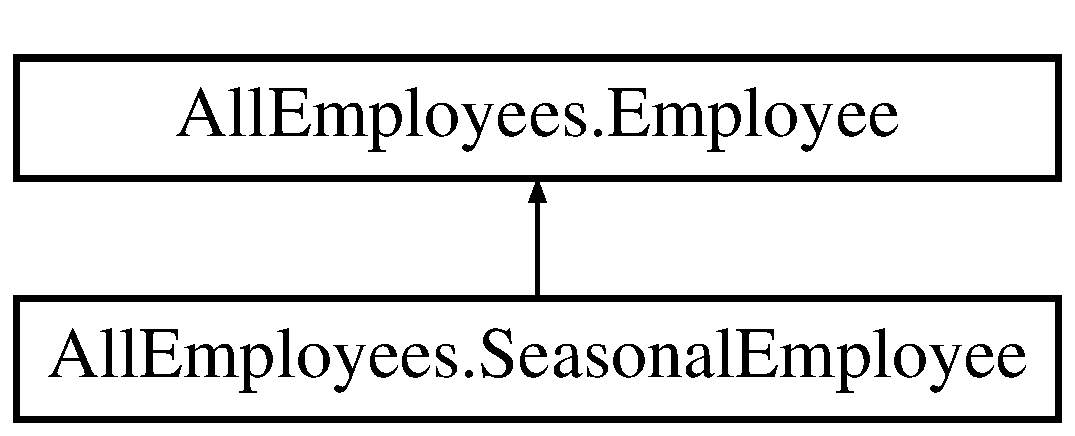
\includegraphics[height=2.000000cm]{class_all_employees_1_1_seasonal_employee}
\end{center}
\end{figure}
\subsection*{Public Member Functions}
\begin{DoxyCompactItemize}
\item 
\hyperlink{class_all_employees_1_1_seasonal_employee_a2206a19da96d42cbd56e7fb5d073c7d4}{Seasonal\+Employee} ()
\begin{DoxyCompactList}\small\item\em default constructor. Sets all values to default \end{DoxyCompactList}\item 
\hyperlink{class_all_employees_1_1_seasonal_employee_acc7fb6022faa7594a0e249a8ba89f217}{Seasonal\+Employee} (string first\+Name, string last\+Name)
\begin{DoxyCompactList}\small\item\em overloaded constructor. Sets name to inputed names, set all other values to default \end{DoxyCompactList}\item 
\hyperlink{class_all_employees_1_1_seasonal_employee_a11c78ec2f72bdeb29d71d48497e34c63}{Seasonal\+Employee} (string first\+Name, string last\+Name, int social\+Insurance\+Number, Date\+Time date\+Of\+Birth, string season, float piece\+Pay)
\begin{DoxyCompactList}\small\item\em overloaded constructor. Sets all values to the values given. no default values \end{DoxyCompactList}\item 
bool \hyperlink{class_all_employees_1_1_seasonal_employee_a70f911ac43a67b84f93ead74860bb6d9}{Validate} ()
\begin{DoxyCompactList}\small\item\em Used to determine in the object contains a valid employee. \end{DoxyCompactList}\item 
string \hyperlink{class_all_employees_1_1_seasonal_employee_a0474e4afe0e11f4e2dd0a523bff3034b}{Details} ()
\begin{DoxyCompactList}\small\item\em Used to print all employee data to the consol. \end{DoxyCompactList}\item 
override string \hyperlink{class_all_employees_1_1_seasonal_employee_a797da83b3ef0a5e7fb04fc5b0d373a11}{To\+String} ()
\begin{DoxyCompactList}\small\item\em Overriden method To\+String used to return a formated string of all data. \end{DoxyCompactList}\item 
bool \hyperlink{class_all_employees_1_1_seasonal_employee_a3cefc2899365780dd013b990ef46326c}{Set\+Season} (string season)
\begin{DoxyCompactList}\small\item\em Setter for season. \end{DoxyCompactList}\item 
bool \hyperlink{class_all_employees_1_1_seasonal_employee_a983e9f6a2a1fd71ed056d8b50d787e88}{Set\+Piece\+Pay} (float piece\+Pay)
\begin{DoxyCompactList}\small\item\em Setter for piece\+Pay. \end{DoxyCompactList}\item 
string \hyperlink{class_all_employees_1_1_seasonal_employee_a189a882ddc11648f3df82e5c0acd5522}{Get\+Season} ()
\begin{DoxyCompactList}\small\item\em Getter for season. \end{DoxyCompactList}\item 
float \hyperlink{class_all_employees_1_1_seasonal_employee_ae7836e968d20baba7327577807d36aa7}{Get\+Piece\+Pay} ()
\begin{DoxyCompactList}\small\item\em Getter for piece\+Pay. \end{DoxyCompactList}\end{DoxyCompactItemize}
\subsection*{Private Attributes}
\begin{DoxyCompactItemize}
\item 
\hypertarget{class_all_employees_1_1_seasonal_employee_a7615ccd677faed6b26afa27aadd7a71e}{}string {\bfseries season}\label{class_all_employees_1_1_seasonal_employee_a7615ccd677faed6b26afa27aadd7a71e}

\item 
\hypertarget{class_all_employees_1_1_seasonal_employee_afc65d49c016c4510e123b93c9570b639}{}float {\bfseries piece\+Pay}\label{class_all_employees_1_1_seasonal_employee_afc65d49c016c4510e123b93c9570b639}

\end{DoxyCompactItemize}
\subsection*{Additional Inherited Members}


\subsection{Detailed Description}
{\bfseries Brief Description} The Seasonal \hyperlink{class_all_employees_1_1_employee}{Employee} class is used to store and manage data about a employee who is hired for a season. This class is a child to \hyperlink{class_all_employees_1_1_employee}{Employee} class. It adds the season the employee is hired for and how much the employee is paid per item completed/created. 

\begin{DoxyAuthor}{Author}
{\itshape Brandon} 
\end{DoxyAuthor}


\subsection{Constructor \& Destructor Documentation}
\hypertarget{class_all_employees_1_1_seasonal_employee_a2206a19da96d42cbd56e7fb5d073c7d4}{}\index{All\+Employees\+::\+Seasonal\+Employee@{All\+Employees\+::\+Seasonal\+Employee}!Seasonal\+Employee@{Seasonal\+Employee}}
\index{Seasonal\+Employee@{Seasonal\+Employee}!All\+Employees\+::\+Seasonal\+Employee@{All\+Employees\+::\+Seasonal\+Employee}}
\subsubsection[{Seasonal\+Employee}]{\setlength{\rightskip}{0pt plus 5cm}All\+Employees.\+Seasonal\+Employee.\+Seasonal\+Employee (
\begin{DoxyParamCaption}
{}
\end{DoxyParamCaption}
)}\label{class_all_employees_1_1_seasonal_employee_a2206a19da96d42cbd56e7fb5d073c7d4}


default constructor. Sets all values to default 

{\bfseries Details}


\begin{DoxyParams}{Parameters}
{\em n/a} & \\
\hline
\end{DoxyParams}
\begin{DoxyReturn}{Returns}
n/a 
\end{DoxyReturn}
\hypertarget{class_all_employees_1_1_seasonal_employee_acc7fb6022faa7594a0e249a8ba89f217}{}\index{All\+Employees\+::\+Seasonal\+Employee@{All\+Employees\+::\+Seasonal\+Employee}!Seasonal\+Employee@{Seasonal\+Employee}}
\index{Seasonal\+Employee@{Seasonal\+Employee}!All\+Employees\+::\+Seasonal\+Employee@{All\+Employees\+::\+Seasonal\+Employee}}
\subsubsection[{Seasonal\+Employee}]{\setlength{\rightskip}{0pt plus 5cm}All\+Employees.\+Seasonal\+Employee.\+Seasonal\+Employee (
\begin{DoxyParamCaption}
\item[{string}]{first\+Name, }
\item[{string}]{last\+Name}
\end{DoxyParamCaption}
)}\label{class_all_employees_1_1_seasonal_employee_acc7fb6022faa7594a0e249a8ba89f217}


overloaded constructor. Sets name to inputed names, set all other values to default 

{\bfseries Details}


\begin{DoxyParams}{Parameters}
{\em first\+Name} & -\/ {\bfseries string} -\/ First Name of employee to add to records \\
\hline
{\em last\+Name} & -\/ {\bfseries string} -\/ Last Name of employee to add to records\\
\hline
\end{DoxyParams}

\begin{DoxyExceptions}{Exceptions}
{\em $<$\+Failed\+Constructor\+Exception$>$} & -\/ If the constructor failed to create the object\\
\hline
\end{DoxyExceptions}
\begin{DoxyReturn}{Returns}
n/a 
\end{DoxyReturn}
\hypertarget{class_all_employees_1_1_seasonal_employee_a11c78ec2f72bdeb29d71d48497e34c63}{}\index{All\+Employees\+::\+Seasonal\+Employee@{All\+Employees\+::\+Seasonal\+Employee}!Seasonal\+Employee@{Seasonal\+Employee}}
\index{Seasonal\+Employee@{Seasonal\+Employee}!All\+Employees\+::\+Seasonal\+Employee@{All\+Employees\+::\+Seasonal\+Employee}}
\subsubsection[{Seasonal\+Employee}]{\setlength{\rightskip}{0pt plus 5cm}All\+Employees.\+Seasonal\+Employee.\+Seasonal\+Employee (
\begin{DoxyParamCaption}
\item[{string}]{first\+Name, }
\item[{string}]{last\+Name, }
\item[{int}]{social\+Insurance\+Number, }
\item[{Date\+Time}]{date\+Of\+Birth, }
\item[{string}]{season, }
\item[{float}]{piece\+Pay}
\end{DoxyParamCaption}
)}\label{class_all_employees_1_1_seasonal_employee_a11c78ec2f72bdeb29d71d48497e34c63}


overloaded constructor. Sets all values to the values given. no default values 

{\bfseries Details}


\begin{DoxyParams}{Parameters}
{\em first\+Name} & -\/ {\bfseries string} -\/ First Name of employee to add to records \\
\hline
{\em last\+Name} & -\/ {\bfseries string} -\/ Last Name of employee to add to records \\
\hline
{\em social\+Insurance\+Number} & -\/ {\bfseries int} -\/ Social Insurance Number of employee to add to records \\
\hline
{\em date\+Of\+Birth} & -\/ {\bfseries Date\+Time} -\/ Date Of Birth of employee to add to records \\
\hline
{\em season} & -\/ {\bfseries string} -\/ season the employee worked/works \\
\hline
{\em piece\+Pay} & -\/ {\bfseries float} -\/ the price per unit that the worker is payed\\
\hline
\end{DoxyParams}

\begin{DoxyExceptions}{Exceptions}
{\em $<$\+Failed\+Constructor\+Exception$>$} & -\/ If the constructor failed to create the object\\
\hline
\end{DoxyExceptions}
\begin{DoxyReturn}{Returns}
n/a 
\end{DoxyReturn}


\subsection{Member Function Documentation}
\hypertarget{class_all_employees_1_1_seasonal_employee_a0474e4afe0e11f4e2dd0a523bff3034b}{}\index{All\+Employees\+::\+Seasonal\+Employee@{All\+Employees\+::\+Seasonal\+Employee}!Details@{Details}}
\index{Details@{Details}!All\+Employees\+::\+Seasonal\+Employee@{All\+Employees\+::\+Seasonal\+Employee}}
\subsubsection[{Details}]{\setlength{\rightskip}{0pt plus 5cm}string All\+Employees.\+Seasonal\+Employee.\+Details (
\begin{DoxyParamCaption}
{}
\end{DoxyParamCaption}
)}\label{class_all_employees_1_1_seasonal_employee_a0474e4afe0e11f4e2dd0a523bff3034b}


Used to print all employee data to the consol. 

{\bfseries Details}


\begin{DoxyParams}{Parameters}
{\em n/a} & \\
\hline
\end{DoxyParams}
\begin{DoxyReturn}{Returns}
user\+Info {\bfseries string} -\/ formatted string of employee data 
\end{DoxyReturn}
\hypertarget{class_all_employees_1_1_seasonal_employee_ae7836e968d20baba7327577807d36aa7}{}\index{All\+Employees\+::\+Seasonal\+Employee@{All\+Employees\+::\+Seasonal\+Employee}!Get\+Piece\+Pay@{Get\+Piece\+Pay}}
\index{Get\+Piece\+Pay@{Get\+Piece\+Pay}!All\+Employees\+::\+Seasonal\+Employee@{All\+Employees\+::\+Seasonal\+Employee}}
\subsubsection[{Get\+Piece\+Pay}]{\setlength{\rightskip}{0pt plus 5cm}float All\+Employees.\+Seasonal\+Employee.\+Get\+Piece\+Pay (
\begin{DoxyParamCaption}
{}
\end{DoxyParamCaption}
)}\label{class_all_employees_1_1_seasonal_employee_ae7836e968d20baba7327577807d36aa7}


Getter for piece\+Pay. 

{\bfseries Details}


\begin{DoxyParams}{Parameters}
{\em n/a} & \\
\hline
\end{DoxyParams}
\begin{DoxyReturn}{Returns}
piece\+Pay {\bfseries float} 
\end{DoxyReturn}
\hypertarget{class_all_employees_1_1_seasonal_employee_a189a882ddc11648f3df82e5c0acd5522}{}\index{All\+Employees\+::\+Seasonal\+Employee@{All\+Employees\+::\+Seasonal\+Employee}!Get\+Season@{Get\+Season}}
\index{Get\+Season@{Get\+Season}!All\+Employees\+::\+Seasonal\+Employee@{All\+Employees\+::\+Seasonal\+Employee}}
\subsubsection[{Get\+Season}]{\setlength{\rightskip}{0pt plus 5cm}string All\+Employees.\+Seasonal\+Employee.\+Get\+Season (
\begin{DoxyParamCaption}
{}
\end{DoxyParamCaption}
)}\label{class_all_employees_1_1_seasonal_employee_a189a882ddc11648f3df82e5c0acd5522}


Getter for season. 

{\bfseries Details}


\begin{DoxyParams}{Parameters}
{\em n/a} & \\
\hline
\end{DoxyParams}
\begin{DoxyReturn}{Returns}
season {\bfseries string} 
\end{DoxyReturn}
\hypertarget{class_all_employees_1_1_seasonal_employee_a983e9f6a2a1fd71ed056d8b50d787e88}{}\index{All\+Employees\+::\+Seasonal\+Employee@{All\+Employees\+::\+Seasonal\+Employee}!Set\+Piece\+Pay@{Set\+Piece\+Pay}}
\index{Set\+Piece\+Pay@{Set\+Piece\+Pay}!All\+Employees\+::\+Seasonal\+Employee@{All\+Employees\+::\+Seasonal\+Employee}}
\subsubsection[{Set\+Piece\+Pay}]{\setlength{\rightskip}{0pt plus 5cm}bool All\+Employees.\+Seasonal\+Employee.\+Set\+Piece\+Pay (
\begin{DoxyParamCaption}
\item[{float}]{piece\+Pay}
\end{DoxyParamCaption}
)}\label{class_all_employees_1_1_seasonal_employee_a983e9f6a2a1fd71ed056d8b50d787e88}


Setter for piece\+Pay. 

{\bfseries Details}


\begin{DoxyParams}{Parameters}
{\em piece\+Pay} & {\bfseries float} -\/ The price the employee is payed for each unit created\\
\hline
\end{DoxyParams}
\begin{DoxyReturn}{Returns}
data\+Saved {\bfseries bool} -\/ true if input was valid and data was changed. False it data was not changed 
\end{DoxyReturn}
\hypertarget{class_all_employees_1_1_seasonal_employee_a3cefc2899365780dd013b990ef46326c}{}\index{All\+Employees\+::\+Seasonal\+Employee@{All\+Employees\+::\+Seasonal\+Employee}!Set\+Season@{Set\+Season}}
\index{Set\+Season@{Set\+Season}!All\+Employees\+::\+Seasonal\+Employee@{All\+Employees\+::\+Seasonal\+Employee}}
\subsubsection[{Set\+Season}]{\setlength{\rightskip}{0pt plus 5cm}bool All\+Employees.\+Seasonal\+Employee.\+Set\+Season (
\begin{DoxyParamCaption}
\item[{string}]{season}
\end{DoxyParamCaption}
)}\label{class_all_employees_1_1_seasonal_employee_a3cefc2899365780dd013b990ef46326c}


Setter for season. 

{\bfseries Details}


\begin{DoxyParams}{Parameters}
{\em season} & {\bfseries string} -\/ The season the employee worked/works in\\
\hline
\end{DoxyParams}
\begin{DoxyReturn}{Returns}
data\+Saved {\bfseries bool} -\/ true if input was valid and data was changed. False it data was not changed 
\end{DoxyReturn}
\hypertarget{class_all_employees_1_1_seasonal_employee_a797da83b3ef0a5e7fb04fc5b0d373a11}{}\index{All\+Employees\+::\+Seasonal\+Employee@{All\+Employees\+::\+Seasonal\+Employee}!To\+String@{To\+String}}
\index{To\+String@{To\+String}!All\+Employees\+::\+Seasonal\+Employee@{All\+Employees\+::\+Seasonal\+Employee}}
\subsubsection[{To\+String}]{\setlength{\rightskip}{0pt plus 5cm}override string All\+Employees.\+Seasonal\+Employee.\+To\+String (
\begin{DoxyParamCaption}
{}
\end{DoxyParamCaption}
)}\label{class_all_employees_1_1_seasonal_employee_a797da83b3ef0a5e7fb04fc5b0d373a11}


Overriden method To\+String used to return a formated string of all data. 

{\bfseries Details}


\begin{DoxyParams}{Parameters}
{\em n/a} & \\
\hline
\end{DoxyParams}
\begin{DoxyReturn}{Returns}
employee\+String {\bfseries string} -\/ the formated string containing all employee data 
\end{DoxyReturn}
\hypertarget{class_all_employees_1_1_seasonal_employee_a70f911ac43a67b84f93ead74860bb6d9}{}\index{All\+Employees\+::\+Seasonal\+Employee@{All\+Employees\+::\+Seasonal\+Employee}!Validate@{Validate}}
\index{Validate@{Validate}!All\+Employees\+::\+Seasonal\+Employee@{All\+Employees\+::\+Seasonal\+Employee}}
\subsubsection[{Validate}]{\setlength{\rightskip}{0pt plus 5cm}bool All\+Employees.\+Seasonal\+Employee.\+Validate (
\begin{DoxyParamCaption}
{}
\end{DoxyParamCaption}
)}\label{class_all_employees_1_1_seasonal_employee_a70f911ac43a67b84f93ead74860bb6d9}


Used to determine in the object contains a valid employee. 

{\bfseries Details}


\begin{DoxyParams}{Parameters}
{\em n/a} & \\
\hline
\end{DoxyParams}
\begin{DoxyReturn}{Returns}
data\+Valid -\/ {\bfseries bool} -\/ True if the object contains all data for a valid employee 
\end{DoxyReturn}


The documentation for this class was generated from the following file\+:\begin{DoxyCompactItemize}
\item 
C\+:/\+S\+E\+T\+Repo/trunk/\+E\+M\+S/trunk/\+All\+Employees/\+All\+Employees/Seasonal\+Employee.\+cs\end{DoxyCompactItemize}

\hypertarget{class_my_all_employee_1_1_tests_1_1_seasonal_employee_tests}{}\section{My\+All\+Employee.\+Tests.\+Seasonal\+Employee\+Tests Class Reference}
\label{class_my_all_employee_1_1_tests_1_1_seasonal_employee_tests}\index{My\+All\+Employee.\+Tests.\+Seasonal\+Employee\+Tests@{My\+All\+Employee.\+Tests.\+Seasonal\+Employee\+Tests}}


{\bfseries  Brief Description} This class is used to test the Seasonal\+Employee methods in the All\+Employee class. The methods tested include the constructors, Details, Set\+Date\+Of\+Birth (all 3 overloaded methods), Set\+Piece\+Pay, Set\+Season and To\+String.  


\subsection*{Public Member Functions}
\begin{DoxyCompactItemize}
\item 
void \hyperlink{class_my_all_employee_1_1_tests_1_1_seasonal_employee_tests_a710b6ac7570bad98db92aa4b614d1cd7}{Constructor\+With\+Names\+Test\+Valid1} ()
\begin{DoxyCompactList}\small\item\em This unit test will check if either name contains anything other than a letter, apostrophe, dash. It will throw an exception if wrong. \end{DoxyCompactList}\item 
void \hyperlink{class_my_all_employee_1_1_tests_1_1_seasonal_employee_tests_afbef5fa6965f0050225b570b04fcfb6e}{Constructor\+With\+Names\+Test\+Valid2} ()
\begin{DoxyCompactList}\small\item\em This unit test will check if either name contains anything other than a letter, apostrophe, dash. It will throw an exception if wrong. \end{DoxyCompactList}\item 
void \hyperlink{class_my_all_employee_1_1_tests_1_1_seasonal_employee_tests_a276d4c45b475da23e370b2f7b49d8e2e}{Constructor\+With\+Names\+Test\+Valid3} ()
\begin{DoxyCompactList}\small\item\em This unit test will check if either name contains anything other than a letter, apostrophe, dash. It will throw an exception if wrong. \end{DoxyCompactList}\item 
void \hyperlink{class_my_all_employee_1_1_tests_1_1_seasonal_employee_tests_a2a3e05cecdf76db17637ec9400429d0c}{Constructor\+With\+Names\+Test\+Invalid\+Slash} ()
\begin{DoxyCompactList}\small\item\em This unit test will check if the constructor will fail and if the string is invalid because it contains a slash. \end{DoxyCompactList}\item 
void \hyperlink{class_my_all_employee_1_1_tests_1_1_seasonal_employee_tests_a02019081a27a0983cb5f7d29c4a72d08}{Constructor\+With\+Names\+Test\+Invalid\+Space} ()
\begin{DoxyCompactList}\small\item\em This unit test will check if the constructor will fail and if the string is invalid because it contains a space. \end{DoxyCompactList}\item 
void \hyperlink{class_my_all_employee_1_1_tests_1_1_seasonal_employee_tests_abfa23c08ce68040bcae1e242fc0f5975}{Constructor\+With\+Names\+Test\+Invalid\+Number} ()
\begin{DoxyCompactList}\small\item\em This unit test will check if the constructor will fail and if the string is invalid because it contains a number. \end{DoxyCompactList}\item 
void \hyperlink{class_my_all_employee_1_1_tests_1_1_seasonal_employee_tests_a8826a44d6b6503ac9aabee48ce9608a1}{Constructor\+With\+All\+Param\+Test\+Valid1} ()
\begin{DoxyCompactList}\small\item\em This unit test will check the constructor that takes in all possible parameters, and give them all valid data. \end{DoxyCompactList}\item 
void \hyperlink{class_my_all_employee_1_1_tests_1_1_seasonal_employee_tests_a3f861b922051a6e01c3ec63d757fb85a}{Constructor\+With\+All\+Param\+Test\+Valid2} ()
\begin{DoxyCompactList}\small\item\em This unit test will check the constructor that takes in all possible parameters, and give them all valid data. \end{DoxyCompactList}\item 
void \hyperlink{class_my_all_employee_1_1_tests_1_1_seasonal_employee_tests_af230c1fb248f1a3df7c71149cce6ab80}{Constructor\+With\+All\+Param\+Test\+Valid3} ()
\begin{DoxyCompactList}\small\item\em This unit test will check the constructor that takes in all possible parameters, and give them all valid data. \end{DoxyCompactList}\item 
void \hyperlink{class_my_all_employee_1_1_tests_1_1_seasonal_employee_tests_a65d59f8372d3ceea5eb45168dfb61aed}{Constructor\+With\+All\+Param\+Test\+Invalid\+S\+I\+N} ()
\begin{DoxyCompactList}\small\item\em This unit test will check the constructor that takes in all possible parameters, and give them all invalid data. \end{DoxyCompactList}\item 
void \hyperlink{class_my_all_employee_1_1_tests_1_1_seasonal_employee_tests_add552af166838e9aa1f0c3f2f58b50ae}{Constructor\+With\+All\+Param\+Test\+Invalid\+Piece\+Pay} ()
\begin{DoxyCompactList}\small\item\em This unit test will check the constructor that takes in all possible parameters, and give them all invalid data. \end{DoxyCompactList}\item 
void \hyperlink{class_my_all_employee_1_1_tests_1_1_seasonal_employee_tests_ab37732a0aebe30a6c1764252a0bea3bf}{Constructor\+With\+All\+Param\+Test\+Invalid\+Season} ()
\begin{DoxyCompactList}\small\item\em This unit test will check the constructor that takes in all possible parameters, and give them all invalid data. \end{DoxyCompactList}\item 
void \hyperlink{class_my_all_employee_1_1_tests_1_1_seasonal_employee_tests_a71d96e76f23a2ba0addbf83c6b969d52}{Details\+Test\+Valid} ()
\begin{DoxyCompactList}\small\item\em This unit test will create an employee and runs it\textquotesingle{}s details, and will ensure that the string is what it should be(it is hardcoded) \end{DoxyCompactList}\item 
void \hyperlink{class_my_all_employee_1_1_tests_1_1_seasonal_employee_tests_a712de60d04295ef05d220830954574a7}{To\+String\+Test\+Valid} ()
\begin{DoxyCompactList}\small\item\em This unit test will create an employee and runs it\textquotesingle{}s details, and will ensure that the string is what it should be(it is hardcoded) \end{DoxyCompactList}\item 
void \hyperlink{class_my_all_employee_1_1_tests_1_1_seasonal_employee_tests_ab39595d763f315b9071db67af4ddfdb5}{Set\+Piece\+Pay\+Valid} ()
\begin{DoxyCompactList}\small\item\em This unit test will set the piece pay to a valid amount. \end{DoxyCompactList}\item 
void \hyperlink{class_my_all_employee_1_1_tests_1_1_seasonal_employee_tests_a54b31e16c0b0dc7a6167aa95f03bde9d}{Set\+Piece\+Pay\+Invalid\+Negitive} ()
\begin{DoxyCompactList}\small\item\em This unit test will set the piece pay to an invalid amount. \end{DoxyCompactList}\item 
void \hyperlink{class_my_all_employee_1_1_tests_1_1_seasonal_employee_tests_a72be7ca2a79c9a27833e3551b851a3ff}{Set\+Season\+Valid1} ()
\begin{DoxyCompactList}\small\item\em This unit test will set the season to a valid season. \end{DoxyCompactList}\item 
void \hyperlink{class_my_all_employee_1_1_tests_1_1_seasonal_employee_tests_a425089350805a527c370ea0d0dbc86b8}{Set\+Season\+Valid2} ()
\begin{DoxyCompactList}\small\item\em This unit test will set the season to a valid season. \end{DoxyCompactList}\item 
void \hyperlink{class_my_all_employee_1_1_tests_1_1_seasonal_employee_tests_ac8de2e85a667cbaaccec0f188b47a730}{Set\+Season\+Valid3} ()
\begin{DoxyCompactList}\small\item\em This unit test will set the season to a valid season. \end{DoxyCompactList}\item 
void \hyperlink{class_my_all_employee_1_1_tests_1_1_seasonal_employee_tests_ab03b203538d9d28227f5ae3fcd2d1394}{Set\+Season\+Invalid} ()
\begin{DoxyCompactList}\small\item\em This unit test will set the season to an invalid season. \end{DoxyCompactList}\end{DoxyCompactItemize}


\subsection{Detailed Description}
{\bfseries  Brief Description} This class is used to test the Seasonal\+Employee methods in the All\+Employee class. The methods tested include the constructors, Details, Set\+Date\+Of\+Birth (all 3 overloaded methods), Set\+Piece\+Pay, Set\+Season and To\+String. 

\subsection{Member Function Documentation}
\hypertarget{class_my_all_employee_1_1_tests_1_1_seasonal_employee_tests_add552af166838e9aa1f0c3f2f58b50ae}{}\index{My\+All\+Employee\+::\+Tests\+::\+Seasonal\+Employee\+Tests@{My\+All\+Employee\+::\+Tests\+::\+Seasonal\+Employee\+Tests}!Constructor\+With\+All\+Param\+Test\+Invalid\+Piece\+Pay@{Constructor\+With\+All\+Param\+Test\+Invalid\+Piece\+Pay}}
\index{Constructor\+With\+All\+Param\+Test\+Invalid\+Piece\+Pay@{Constructor\+With\+All\+Param\+Test\+Invalid\+Piece\+Pay}!My\+All\+Employee\+::\+Tests\+::\+Seasonal\+Employee\+Tests@{My\+All\+Employee\+::\+Tests\+::\+Seasonal\+Employee\+Tests}}
\subsubsection[{Constructor\+With\+All\+Param\+Test\+Invalid\+Piece\+Pay}]{\setlength{\rightskip}{0pt plus 5cm}void My\+All\+Employee.\+Tests.\+Seasonal\+Employee\+Tests.\+Constructor\+With\+All\+Param\+Test\+Invalid\+Piece\+Pay (
\begin{DoxyParamCaption}
{}
\end{DoxyParamCaption}
)}\label{class_my_all_employee_1_1_tests_1_1_seasonal_employee_tests_add552af166838e9aa1f0c3f2f58b50ae}


This unit test will check the constructor that takes in all possible parameters, and give them all invalid data. 

\textbackslash{} {\bfseries  Name of Method} \hyperlink{class_my_all_employee_1_1_tests_1_1_seasonal_employee_tests_add552af166838e9aa1f0c3f2f58b50ae}{Constructor\+With\+All\+Param\+Test\+Invalid\+Piece\+Pay()}

\textbackslash{} {\bfseries  How test is Conducted} This test is run automatically

\textbackslash{} {\bfseries  Type of Test} The type of test is an exception.

\textbackslash{} {\bfseries  Sample Data Sets} Date\+Time D\+O\+B = new Date\+Time(1993, 04, 24); \char`\"{}\+Brandon\char`\"{}, \char`\"{}\+Davies\char`\"{}, 1234756789, D\+O\+B,\char`\"{}\+Fall\char`\"{}, -\/12

\textbackslash{} {\bfseries  Expected Result} The expected result is that there is an exception

\textbackslash{} {\bfseries  Actual Result} An exception is thrown \hypertarget{class_my_all_employee_1_1_tests_1_1_seasonal_employee_tests_ab37732a0aebe30a6c1764252a0bea3bf}{}\index{My\+All\+Employee\+::\+Tests\+::\+Seasonal\+Employee\+Tests@{My\+All\+Employee\+::\+Tests\+::\+Seasonal\+Employee\+Tests}!Constructor\+With\+All\+Param\+Test\+Invalid\+Season@{Constructor\+With\+All\+Param\+Test\+Invalid\+Season}}
\index{Constructor\+With\+All\+Param\+Test\+Invalid\+Season@{Constructor\+With\+All\+Param\+Test\+Invalid\+Season}!My\+All\+Employee\+::\+Tests\+::\+Seasonal\+Employee\+Tests@{My\+All\+Employee\+::\+Tests\+::\+Seasonal\+Employee\+Tests}}
\subsubsection[{Constructor\+With\+All\+Param\+Test\+Invalid\+Season}]{\setlength{\rightskip}{0pt plus 5cm}void My\+All\+Employee.\+Tests.\+Seasonal\+Employee\+Tests.\+Constructor\+With\+All\+Param\+Test\+Invalid\+Season (
\begin{DoxyParamCaption}
{}
\end{DoxyParamCaption}
)}\label{class_my_all_employee_1_1_tests_1_1_seasonal_employee_tests_ab37732a0aebe30a6c1764252a0bea3bf}


This unit test will check the constructor that takes in all possible parameters, and give them all invalid data. 

\textbackslash{} {\bfseries  Name of Method} \hyperlink{class_my_all_employee_1_1_tests_1_1_seasonal_employee_tests_ab37732a0aebe30a6c1764252a0bea3bf}{Constructor\+With\+All\+Param\+Test\+Invalid\+Season()}

\textbackslash{} {\bfseries  How test is Conducted} This test is run automatically

\textbackslash{} {\bfseries  Type of Test} The type of test is an exception.

\textbackslash{} {\bfseries  Sample Data Sets} Date\+Time D\+O\+B = new Date\+Time(1993, 04, 24); \char`\"{}\+Brandon\char`\"{}, \char`\"{}\+Davies\char`\"{}, 1234756789, D\+O\+B,\char`\"{}\+October\char`\"{}, 13

\textbackslash{} {\bfseries  Expected Result} The expected result is that there is an exception

\textbackslash{} {\bfseries  Actual Result} An exception is thrown \hypertarget{class_my_all_employee_1_1_tests_1_1_seasonal_employee_tests_a65d59f8372d3ceea5eb45168dfb61aed}{}\index{My\+All\+Employee\+::\+Tests\+::\+Seasonal\+Employee\+Tests@{My\+All\+Employee\+::\+Tests\+::\+Seasonal\+Employee\+Tests}!Constructor\+With\+All\+Param\+Test\+Invalid\+S\+I\+N@{Constructor\+With\+All\+Param\+Test\+Invalid\+S\+I\+N}}
\index{Constructor\+With\+All\+Param\+Test\+Invalid\+S\+I\+N@{Constructor\+With\+All\+Param\+Test\+Invalid\+S\+I\+N}!My\+All\+Employee\+::\+Tests\+::\+Seasonal\+Employee\+Tests@{My\+All\+Employee\+::\+Tests\+::\+Seasonal\+Employee\+Tests}}
\subsubsection[{Constructor\+With\+All\+Param\+Test\+Invalid\+S\+I\+N}]{\setlength{\rightskip}{0pt plus 5cm}void My\+All\+Employee.\+Tests.\+Seasonal\+Employee\+Tests.\+Constructor\+With\+All\+Param\+Test\+Invalid\+S\+I\+N (
\begin{DoxyParamCaption}
{}
\end{DoxyParamCaption}
)}\label{class_my_all_employee_1_1_tests_1_1_seasonal_employee_tests_a65d59f8372d3ceea5eb45168dfb61aed}


This unit test will check the constructor that takes in all possible parameters, and give them all invalid data. 

\textbackslash{} {\bfseries  Name of Method} \hyperlink{class_my_all_employee_1_1_tests_1_1_seasonal_employee_tests_a65d59f8372d3ceea5eb45168dfb61aed}{Constructor\+With\+All\+Param\+Test\+Invalid\+S\+I\+N()}

\textbackslash{} {\bfseries  How test is Conducted} This test is run automatically

\textbackslash{} {\bfseries  Type of Test} The type of test is an exception.

\textbackslash{} {\bfseries  Sample Data Sets} Date\+Time D\+O\+B = new Date\+Time(1993, 04, 24); \char`\"{}\+Brandon\char`\"{}, \char`\"{}\+Davies\char`\"{}, 1234756789, D\+O\+B, \char`\"{}\+Fall\char`\"{}, 10

\textbackslash{} {\bfseries  Expected Result} The expected result is that there is an exception

\textbackslash{} {\bfseries  Actual Result} An exception is thrown \hypertarget{class_my_all_employee_1_1_tests_1_1_seasonal_employee_tests_a8826a44d6b6503ac9aabee48ce9608a1}{}\index{My\+All\+Employee\+::\+Tests\+::\+Seasonal\+Employee\+Tests@{My\+All\+Employee\+::\+Tests\+::\+Seasonal\+Employee\+Tests}!Constructor\+With\+All\+Param\+Test\+Valid1@{Constructor\+With\+All\+Param\+Test\+Valid1}}
\index{Constructor\+With\+All\+Param\+Test\+Valid1@{Constructor\+With\+All\+Param\+Test\+Valid1}!My\+All\+Employee\+::\+Tests\+::\+Seasonal\+Employee\+Tests@{My\+All\+Employee\+::\+Tests\+::\+Seasonal\+Employee\+Tests}}
\subsubsection[{Constructor\+With\+All\+Param\+Test\+Valid1}]{\setlength{\rightskip}{0pt plus 5cm}void My\+All\+Employee.\+Tests.\+Seasonal\+Employee\+Tests.\+Constructor\+With\+All\+Param\+Test\+Valid1 (
\begin{DoxyParamCaption}
{}
\end{DoxyParamCaption}
)}\label{class_my_all_employee_1_1_tests_1_1_seasonal_employee_tests_a8826a44d6b6503ac9aabee48ce9608a1}


This unit test will check the constructor that takes in all possible parameters, and give them all valid data. 

\textbackslash{} {\bfseries  Name of Method} \hyperlink{class_my_all_employee_1_1_tests_1_1_seasonal_employee_tests_a8826a44d6b6503ac9aabee48ce9608a1}{Constructor\+With\+All\+Param\+Test\+Valid1()}

\textbackslash{} {\bfseries  How test is Conducted} This test is run automatically

\textbackslash{} {\bfseries  Type of Test} The type of test is an normal/function.

\textbackslash{} {\bfseries  Sample Data Sets} Date\+Time D\+O\+B = new Date\+Time(1993, 04, 24); \char`\"{}\+Brandon\char`\"{}, \char`\"{}\+Davies\char`\"{}, 123456789, D\+O\+B, D\+O\+H, \char`\"{}\+Summer\char`\"{}, 10

\textbackslash{} {\bfseries  Expected Result} The expected result is that there is no exception

\textbackslash{} {\bfseries  Actual Result} An exception is not thrown \hypertarget{class_my_all_employee_1_1_tests_1_1_seasonal_employee_tests_a3f861b922051a6e01c3ec63d757fb85a}{}\index{My\+All\+Employee\+::\+Tests\+::\+Seasonal\+Employee\+Tests@{My\+All\+Employee\+::\+Tests\+::\+Seasonal\+Employee\+Tests}!Constructor\+With\+All\+Param\+Test\+Valid2@{Constructor\+With\+All\+Param\+Test\+Valid2}}
\index{Constructor\+With\+All\+Param\+Test\+Valid2@{Constructor\+With\+All\+Param\+Test\+Valid2}!My\+All\+Employee\+::\+Tests\+::\+Seasonal\+Employee\+Tests@{My\+All\+Employee\+::\+Tests\+::\+Seasonal\+Employee\+Tests}}
\subsubsection[{Constructor\+With\+All\+Param\+Test\+Valid2}]{\setlength{\rightskip}{0pt plus 5cm}void My\+All\+Employee.\+Tests.\+Seasonal\+Employee\+Tests.\+Constructor\+With\+All\+Param\+Test\+Valid2 (
\begin{DoxyParamCaption}
{}
\end{DoxyParamCaption}
)}\label{class_my_all_employee_1_1_tests_1_1_seasonal_employee_tests_a3f861b922051a6e01c3ec63d757fb85a}


This unit test will check the constructor that takes in all possible parameters, and give them all valid data. 

\textbackslash{} {\bfseries  Name of Method} \hyperlink{class_my_all_employee_1_1_tests_1_1_seasonal_employee_tests_a3f861b922051a6e01c3ec63d757fb85a}{Constructor\+With\+All\+Param\+Test\+Valid2()}

\textbackslash{} {\bfseries  How test is Conducted} This test is run automatically

\textbackslash{} {\bfseries  Type of Test} The type of test is an normal/function.

\textbackslash{} {\bfseries  Sample Data Sets} Date\+Time D\+O\+B = new Date\+Time(1991, 12, 23); \char`\"{}\+Brandon\char`\"{}, \char`\"{}\+Mc\textquotesingle{}\+Davies\char`\"{}, 123456789, D\+O\+B, \char`\"{}\+Winter\char`\"{}, 15

\textbackslash{} {\bfseries  Expected Result} The expected result is that there is no exception

\textbackslash{} {\bfseries  Actual Result} An exception is not thrown \hypertarget{class_my_all_employee_1_1_tests_1_1_seasonal_employee_tests_af230c1fb248f1a3df7c71149cce6ab80}{}\index{My\+All\+Employee\+::\+Tests\+::\+Seasonal\+Employee\+Tests@{My\+All\+Employee\+::\+Tests\+::\+Seasonal\+Employee\+Tests}!Constructor\+With\+All\+Param\+Test\+Valid3@{Constructor\+With\+All\+Param\+Test\+Valid3}}
\index{Constructor\+With\+All\+Param\+Test\+Valid3@{Constructor\+With\+All\+Param\+Test\+Valid3}!My\+All\+Employee\+::\+Tests\+::\+Seasonal\+Employee\+Tests@{My\+All\+Employee\+::\+Tests\+::\+Seasonal\+Employee\+Tests}}
\subsubsection[{Constructor\+With\+All\+Param\+Test\+Valid3}]{\setlength{\rightskip}{0pt plus 5cm}void My\+All\+Employee.\+Tests.\+Seasonal\+Employee\+Tests.\+Constructor\+With\+All\+Param\+Test\+Valid3 (
\begin{DoxyParamCaption}
{}
\end{DoxyParamCaption}
)}\label{class_my_all_employee_1_1_tests_1_1_seasonal_employee_tests_af230c1fb248f1a3df7c71149cce6ab80}


This unit test will check the constructor that takes in all possible parameters, and give them all valid data. 

\textbackslash{} {\bfseries  Name of Method} \hyperlink{class_my_all_employee_1_1_tests_1_1_seasonal_employee_tests_af230c1fb248f1a3df7c71149cce6ab80}{Constructor\+With\+All\+Param\+Test\+Valid3()}

\textbackslash{} {\bfseries  How test is Conducted} This test is run automatically

\textbackslash{} {\bfseries  Type of Test} The type of test is an normal/function.

\textbackslash{} {\bfseries  Sample Data Sets} Date\+Time D\+O\+B = new Date\+Time(1984, 04, 24); \char`\"{}\+Brandon\char`\"{}, \char`\"{}\+Davies\char`\"{}, 123456789, D\+O\+B, \char`\"{}\+Fall\char`\"{}, 1

\textbackslash{} {\bfseries  Expected Result} The expected result is that there is no exception

\textbackslash{} {\bfseries  Actual Result} An exception is not thrown \hypertarget{class_my_all_employee_1_1_tests_1_1_seasonal_employee_tests_abfa23c08ce68040bcae1e242fc0f5975}{}\index{My\+All\+Employee\+::\+Tests\+::\+Seasonal\+Employee\+Tests@{My\+All\+Employee\+::\+Tests\+::\+Seasonal\+Employee\+Tests}!Constructor\+With\+Names\+Test\+Invalid\+Number@{Constructor\+With\+Names\+Test\+Invalid\+Number}}
\index{Constructor\+With\+Names\+Test\+Invalid\+Number@{Constructor\+With\+Names\+Test\+Invalid\+Number}!My\+All\+Employee\+::\+Tests\+::\+Seasonal\+Employee\+Tests@{My\+All\+Employee\+::\+Tests\+::\+Seasonal\+Employee\+Tests}}
\subsubsection[{Constructor\+With\+Names\+Test\+Invalid\+Number}]{\setlength{\rightskip}{0pt plus 5cm}void My\+All\+Employee.\+Tests.\+Seasonal\+Employee\+Tests.\+Constructor\+With\+Names\+Test\+Invalid\+Number (
\begin{DoxyParamCaption}
{}
\end{DoxyParamCaption}
)}\label{class_my_all_employee_1_1_tests_1_1_seasonal_employee_tests_abfa23c08ce68040bcae1e242fc0f5975}


This unit test will check if the constructor will fail and if the string is invalid because it contains a number. 

\textbackslash{} {\bfseries  Name of Method} \hyperlink{class_my_all_employee_1_1_tests_1_1_seasonal_employee_tests_abfa23c08ce68040bcae1e242fc0f5975}{Constructor\+With\+Names\+Test\+Invalid\+Number()}

\textbackslash{} {\bfseries  How test is Conducted} This test is run automatically

\textbackslash{} {\bfseries  Type of Test} The type of test is an exception.

\textbackslash{} {\bfseries  Sample Data Sets} \char`\"{}\+Brandon2\char`\"{}, \char`\"{}\+Davies\char`\"{}

\textbackslash{} {\bfseries  Expected Result} The expected result is that it will throw an exception

\textbackslash{} {\bfseries  Actual Result} An exception is thrown \hypertarget{class_my_all_employee_1_1_tests_1_1_seasonal_employee_tests_a2a3e05cecdf76db17637ec9400429d0c}{}\index{My\+All\+Employee\+::\+Tests\+::\+Seasonal\+Employee\+Tests@{My\+All\+Employee\+::\+Tests\+::\+Seasonal\+Employee\+Tests}!Constructor\+With\+Names\+Test\+Invalid\+Slash@{Constructor\+With\+Names\+Test\+Invalid\+Slash}}
\index{Constructor\+With\+Names\+Test\+Invalid\+Slash@{Constructor\+With\+Names\+Test\+Invalid\+Slash}!My\+All\+Employee\+::\+Tests\+::\+Seasonal\+Employee\+Tests@{My\+All\+Employee\+::\+Tests\+::\+Seasonal\+Employee\+Tests}}
\subsubsection[{Constructor\+With\+Names\+Test\+Invalid\+Slash}]{\setlength{\rightskip}{0pt plus 5cm}void My\+All\+Employee.\+Tests.\+Seasonal\+Employee\+Tests.\+Constructor\+With\+Names\+Test\+Invalid\+Slash (
\begin{DoxyParamCaption}
{}
\end{DoxyParamCaption}
)}\label{class_my_all_employee_1_1_tests_1_1_seasonal_employee_tests_a2a3e05cecdf76db17637ec9400429d0c}


This unit test will check if the constructor will fail and if the string is invalid because it contains a slash. 

\textbackslash{} {\bfseries  Name of Method} \hyperlink{class_my_all_employee_1_1_tests_1_1_seasonal_employee_tests_a2a3e05cecdf76db17637ec9400429d0c}{Constructor\+With\+Names\+Test\+Invalid\+Slash()}

\textbackslash{} {\bfseries  How test is Conducted} This test is run automatically

\textbackslash{} {\bfseries  Type of Test} The type of test is an exception.

\textbackslash{} {\bfseries  Sample Data Sets} \char`\"{}\+Brandon\char`\"{}, \char`\"{}\+Mc/\+Davies\char`\"{}

\textbackslash{} {\bfseries  Expected Result} The expected result is that it will throw an exception

\textbackslash{} {\bfseries  Actual Result} An exception is thrown \hypertarget{class_my_all_employee_1_1_tests_1_1_seasonal_employee_tests_a02019081a27a0983cb5f7d29c4a72d08}{}\index{My\+All\+Employee\+::\+Tests\+::\+Seasonal\+Employee\+Tests@{My\+All\+Employee\+::\+Tests\+::\+Seasonal\+Employee\+Tests}!Constructor\+With\+Names\+Test\+Invalid\+Space@{Constructor\+With\+Names\+Test\+Invalid\+Space}}
\index{Constructor\+With\+Names\+Test\+Invalid\+Space@{Constructor\+With\+Names\+Test\+Invalid\+Space}!My\+All\+Employee\+::\+Tests\+::\+Seasonal\+Employee\+Tests@{My\+All\+Employee\+::\+Tests\+::\+Seasonal\+Employee\+Tests}}
\subsubsection[{Constructor\+With\+Names\+Test\+Invalid\+Space}]{\setlength{\rightskip}{0pt plus 5cm}void My\+All\+Employee.\+Tests.\+Seasonal\+Employee\+Tests.\+Constructor\+With\+Names\+Test\+Invalid\+Space (
\begin{DoxyParamCaption}
{}
\end{DoxyParamCaption}
)}\label{class_my_all_employee_1_1_tests_1_1_seasonal_employee_tests_a02019081a27a0983cb5f7d29c4a72d08}


This unit test will check if the constructor will fail and if the string is invalid because it contains a space. 

\textbackslash{} {\bfseries  Name of Method} \hyperlink{class_my_all_employee_1_1_tests_1_1_seasonal_employee_tests_a02019081a27a0983cb5f7d29c4a72d08}{Constructor\+With\+Names\+Test\+Invalid\+Space()}

\textbackslash{} {\bfseries  How test is Conducted} This test is run automatically

\textbackslash{} {\bfseries  Type of Test} The type of test is an exception.

\textbackslash{} {\bfseries  Sample Data Sets} \char`\"{}\+Brandon\char`\"{}, \char`\"{}\+Mc Davies\char`\"{}

\textbackslash{} {\bfseries  Expected Result} The expected result is that it will throw an exception

\textbackslash{} {\bfseries  Actual Result} An exception is thrown \hypertarget{class_my_all_employee_1_1_tests_1_1_seasonal_employee_tests_a710b6ac7570bad98db92aa4b614d1cd7}{}\index{My\+All\+Employee\+::\+Tests\+::\+Seasonal\+Employee\+Tests@{My\+All\+Employee\+::\+Tests\+::\+Seasonal\+Employee\+Tests}!Constructor\+With\+Names\+Test\+Valid1@{Constructor\+With\+Names\+Test\+Valid1}}
\index{Constructor\+With\+Names\+Test\+Valid1@{Constructor\+With\+Names\+Test\+Valid1}!My\+All\+Employee\+::\+Tests\+::\+Seasonal\+Employee\+Tests@{My\+All\+Employee\+::\+Tests\+::\+Seasonal\+Employee\+Tests}}
\subsubsection[{Constructor\+With\+Names\+Test\+Valid1}]{\setlength{\rightskip}{0pt plus 5cm}void My\+All\+Employee.\+Tests.\+Seasonal\+Employee\+Tests.\+Constructor\+With\+Names\+Test\+Valid1 (
\begin{DoxyParamCaption}
{}
\end{DoxyParamCaption}
)}\label{class_my_all_employee_1_1_tests_1_1_seasonal_employee_tests_a710b6ac7570bad98db92aa4b614d1cd7}


This unit test will check if either name contains anything other than a letter, apostrophe, dash. It will throw an exception if wrong. 

\textbackslash{} {\bfseries  Name of Method} \hyperlink{class_my_all_employee_1_1_tests_1_1_seasonal_employee_tests_a710b6ac7570bad98db92aa4b614d1cd7}{Constructor\+With\+Names\+Test\+Valid1()}

\textbackslash{} {\bfseries  How test is Conducted} This test is run automatically

\textbackslash{} {\bfseries  Type of Test} The type of test is normal/functional.

\textbackslash{} {\bfseries  Sample Data Sets} \char`\"{}\+Brandon\char`\"{}, \char`\"{}\+Davies\char`\"{}

\textbackslash{} {\bfseries  Expected Result} The expected result is that there is no exception

\textbackslash{} {\bfseries  Actual Result} There is no exception. \hypertarget{class_my_all_employee_1_1_tests_1_1_seasonal_employee_tests_afbef5fa6965f0050225b570b04fcfb6e}{}\index{My\+All\+Employee\+::\+Tests\+::\+Seasonal\+Employee\+Tests@{My\+All\+Employee\+::\+Tests\+::\+Seasonal\+Employee\+Tests}!Constructor\+With\+Names\+Test\+Valid2@{Constructor\+With\+Names\+Test\+Valid2}}
\index{Constructor\+With\+Names\+Test\+Valid2@{Constructor\+With\+Names\+Test\+Valid2}!My\+All\+Employee\+::\+Tests\+::\+Seasonal\+Employee\+Tests@{My\+All\+Employee\+::\+Tests\+::\+Seasonal\+Employee\+Tests}}
\subsubsection[{Constructor\+With\+Names\+Test\+Valid2}]{\setlength{\rightskip}{0pt plus 5cm}void My\+All\+Employee.\+Tests.\+Seasonal\+Employee\+Tests.\+Constructor\+With\+Names\+Test\+Valid2 (
\begin{DoxyParamCaption}
{}
\end{DoxyParamCaption}
)}\label{class_my_all_employee_1_1_tests_1_1_seasonal_employee_tests_afbef5fa6965f0050225b570b04fcfb6e}


This unit test will check if either name contains anything other than a letter, apostrophe, dash. It will throw an exception if wrong. 

\textbackslash{} {\bfseries  Name of Method} \hyperlink{class_my_all_employee_1_1_tests_1_1_seasonal_employee_tests_afbef5fa6965f0050225b570b04fcfb6e}{Constructor\+With\+Names\+Test\+Valid2()}

\textbackslash{} {\bfseries  How test is Conducted} This test is run automatically

\textbackslash{} {\bfseries  Type of Test} The type of test is normal/functional.

\textbackslash{} {\bfseries  Sample Data Sets} \char`\"{}\+Brandon\char`\"{}, \char`\"{}\+Mc\textquotesingle{}\+Davies\char`\"{}

\textbackslash{} {\bfseries  Expected Result} The expected result is that there is no exception

\textbackslash{} {\bfseries  Actual Result} There is no exception. \hypertarget{class_my_all_employee_1_1_tests_1_1_seasonal_employee_tests_a276d4c45b475da23e370b2f7b49d8e2e}{}\index{My\+All\+Employee\+::\+Tests\+::\+Seasonal\+Employee\+Tests@{My\+All\+Employee\+::\+Tests\+::\+Seasonal\+Employee\+Tests}!Constructor\+With\+Names\+Test\+Valid3@{Constructor\+With\+Names\+Test\+Valid3}}
\index{Constructor\+With\+Names\+Test\+Valid3@{Constructor\+With\+Names\+Test\+Valid3}!My\+All\+Employee\+::\+Tests\+::\+Seasonal\+Employee\+Tests@{My\+All\+Employee\+::\+Tests\+::\+Seasonal\+Employee\+Tests}}
\subsubsection[{Constructor\+With\+Names\+Test\+Valid3}]{\setlength{\rightskip}{0pt plus 5cm}void My\+All\+Employee.\+Tests.\+Seasonal\+Employee\+Tests.\+Constructor\+With\+Names\+Test\+Valid3 (
\begin{DoxyParamCaption}
{}
\end{DoxyParamCaption}
)}\label{class_my_all_employee_1_1_tests_1_1_seasonal_employee_tests_a276d4c45b475da23e370b2f7b49d8e2e}


This unit test will check if either name contains anything other than a letter, apostrophe, dash. It will throw an exception if wrong. 

\textbackslash{} {\bfseries  Name of Method} \hyperlink{class_my_all_employee_1_1_tests_1_1_seasonal_employee_tests_a276d4c45b475da23e370b2f7b49d8e2e}{Constructor\+With\+Names\+Test\+Valid3()}

\textbackslash{} {\bfseries  How test is Conducted} This test is run automatically

\textbackslash{} {\bfseries  Type of Test} The type of test is normal/functional.

\textbackslash{} {\bfseries  Sample Data Sets} \char`\"{}\+Brandon\char`\"{}, \char`\"{}\+Le\+Roy-\/\+Davies\char`\"{}

\textbackslash{} {\bfseries  Expected Result} The expected result is that there is no exception

\textbackslash{} {\bfseries  Actual Result} There is no exception. \hypertarget{class_my_all_employee_1_1_tests_1_1_seasonal_employee_tests_a71d96e76f23a2ba0addbf83c6b969d52}{}\index{My\+All\+Employee\+::\+Tests\+::\+Seasonal\+Employee\+Tests@{My\+All\+Employee\+::\+Tests\+::\+Seasonal\+Employee\+Tests}!Details\+Test\+Valid@{Details\+Test\+Valid}}
\index{Details\+Test\+Valid@{Details\+Test\+Valid}!My\+All\+Employee\+::\+Tests\+::\+Seasonal\+Employee\+Tests@{My\+All\+Employee\+::\+Tests\+::\+Seasonal\+Employee\+Tests}}
\subsubsection[{Details\+Test\+Valid}]{\setlength{\rightskip}{0pt plus 5cm}void My\+All\+Employee.\+Tests.\+Seasonal\+Employee\+Tests.\+Details\+Test\+Valid (
\begin{DoxyParamCaption}
{}
\end{DoxyParamCaption}
)}\label{class_my_all_employee_1_1_tests_1_1_seasonal_employee_tests_a71d96e76f23a2ba0addbf83c6b969d52}


This unit test will create an employee and runs it\textquotesingle{}s details, and will ensure that the string is what it should be(it is hardcoded) 

\textbackslash{} {\bfseries  Name of Method} \hyperlink{class_my_all_employee_1_1_tests_1_1_seasonal_employee_tests_a71d96e76f23a2ba0addbf83c6b969d52}{Details\+Test\+Valid()}

\textbackslash{} {\bfseries  How test is Conducted} This test is run automatically

\textbackslash{} {\bfseries  Type of Test} The type of test is an normal/function.

\textbackslash{} {\bfseries  Sample Data Sets} Date\+Time D\+O\+B = new Date\+Time(1954, 04, 24); \char`\"{}\+Brandon\char`\"{}, \char`\"{}\+Davies\char`\"{}, 123456789, D\+O\+B, \char`\"{}\+Winter\char`\"{}, 15

\textbackslash{} {\bfseries  Expected Result} The expected result is that the string will be \char`\"{}\+Employee Type\+: Seasonal\textbackslash{}n\+Name\+: Brandon Mc\textquotesingle{}\+Davies\textbackslash{}n\+Social Insurance Number\+: 123 456 789\textbackslash{}n\+Date of Birth\+: 1993-\/04-\/24\textbackslash{}n\+Season\+: Winter\textbackslash{}n\+Price per Piece\+: 15\char`\"{}

\textbackslash{} {\bfseries  Actual Result} The string is equivalent to \char`\"{}\+Employee Type\+: Seasonal\textbackslash{}n\+Name\+: Brandon Mc\textquotesingle{}\+Davies\textbackslash{}n\+Social Insurance Number\+: 123 456 789\textbackslash{}n\+Date of Birth\+: 1993-\/04-\/24\textbackslash{}n\+Season\+: Winter\textbackslash{}n\+Price per Piece\+: 15\char`\"{} \hypertarget{class_my_all_employee_1_1_tests_1_1_seasonal_employee_tests_a54b31e16c0b0dc7a6167aa95f03bde9d}{}\index{My\+All\+Employee\+::\+Tests\+::\+Seasonal\+Employee\+Tests@{My\+All\+Employee\+::\+Tests\+::\+Seasonal\+Employee\+Tests}!Set\+Piece\+Pay\+Invalid\+Negitive@{Set\+Piece\+Pay\+Invalid\+Negitive}}
\index{Set\+Piece\+Pay\+Invalid\+Negitive@{Set\+Piece\+Pay\+Invalid\+Negitive}!My\+All\+Employee\+::\+Tests\+::\+Seasonal\+Employee\+Tests@{My\+All\+Employee\+::\+Tests\+::\+Seasonal\+Employee\+Tests}}
\subsubsection[{Set\+Piece\+Pay\+Invalid\+Negitive}]{\setlength{\rightskip}{0pt plus 5cm}void My\+All\+Employee.\+Tests.\+Seasonal\+Employee\+Tests.\+Set\+Piece\+Pay\+Invalid\+Negitive (
\begin{DoxyParamCaption}
{}
\end{DoxyParamCaption}
)}\label{class_my_all_employee_1_1_tests_1_1_seasonal_employee_tests_a54b31e16c0b0dc7a6167aa95f03bde9d}


This unit test will set the piece pay to an invalid amount. 

\textbackslash{} {\bfseries  Name of Method} \hyperlink{class_my_all_employee_1_1_tests_1_1_seasonal_employee_tests_a54b31e16c0b0dc7a6167aa95f03bde9d}{Set\+Piece\+Pay\+Invalid\+Negitive()}

\textbackslash{} {\bfseries  How test is Conducted} This test is run automatically

\textbackslash{} {\bfseries  Type of Test} The type of test is an exception.

\textbackslash{} {\bfseries  Sample Data Sets} \char`\"{}\+Brandon\char`\"{}, \char`\"{}\+Davies\char`\"{} -\/10

\textbackslash{} {\bfseries  Expected Result} The expected result is the return value should be false and the data member should not have changed

\textbackslash{} {\bfseries  Actual Result} Return value is false, and the data member should not have changed \hypertarget{class_my_all_employee_1_1_tests_1_1_seasonal_employee_tests_ab39595d763f315b9071db67af4ddfdb5}{}\index{My\+All\+Employee\+::\+Tests\+::\+Seasonal\+Employee\+Tests@{My\+All\+Employee\+::\+Tests\+::\+Seasonal\+Employee\+Tests}!Set\+Piece\+Pay\+Valid@{Set\+Piece\+Pay\+Valid}}
\index{Set\+Piece\+Pay\+Valid@{Set\+Piece\+Pay\+Valid}!My\+All\+Employee\+::\+Tests\+::\+Seasonal\+Employee\+Tests@{My\+All\+Employee\+::\+Tests\+::\+Seasonal\+Employee\+Tests}}
\subsubsection[{Set\+Piece\+Pay\+Valid}]{\setlength{\rightskip}{0pt plus 5cm}void My\+All\+Employee.\+Tests.\+Seasonal\+Employee\+Tests.\+Set\+Piece\+Pay\+Valid (
\begin{DoxyParamCaption}
{}
\end{DoxyParamCaption}
)}\label{class_my_all_employee_1_1_tests_1_1_seasonal_employee_tests_ab39595d763f315b9071db67af4ddfdb5}


This unit test will set the piece pay to a valid amount. 

\textbackslash{} {\bfseries  Name of Method} \hyperlink{class_my_all_employee_1_1_tests_1_1_seasonal_employee_tests_ab39595d763f315b9071db67af4ddfdb5}{Set\+Piece\+Pay\+Valid()}

\textbackslash{} {\bfseries  How test is Conducted} This test is run automatically

\textbackslash{} {\bfseries  Type of Test} The type of test is an normal/function.

\textbackslash{} {\bfseries  Sample Data Sets} \char`\"{}\+Brandon\char`\"{}, \char`\"{}\+Davies\char`\"{} 10

\textbackslash{} {\bfseries  Expected Result} The expected result is the return value should be true and the data member should have changed

\textbackslash{} {\bfseries  Actual Result} Return value is true, and the data member should have changed \hypertarget{class_my_all_employee_1_1_tests_1_1_seasonal_employee_tests_ab03b203538d9d28227f5ae3fcd2d1394}{}\index{My\+All\+Employee\+::\+Tests\+::\+Seasonal\+Employee\+Tests@{My\+All\+Employee\+::\+Tests\+::\+Seasonal\+Employee\+Tests}!Set\+Season\+Invalid@{Set\+Season\+Invalid}}
\index{Set\+Season\+Invalid@{Set\+Season\+Invalid}!My\+All\+Employee\+::\+Tests\+::\+Seasonal\+Employee\+Tests@{My\+All\+Employee\+::\+Tests\+::\+Seasonal\+Employee\+Tests}}
\subsubsection[{Set\+Season\+Invalid}]{\setlength{\rightskip}{0pt plus 5cm}void My\+All\+Employee.\+Tests.\+Seasonal\+Employee\+Tests.\+Set\+Season\+Invalid (
\begin{DoxyParamCaption}
{}
\end{DoxyParamCaption}
)}\label{class_my_all_employee_1_1_tests_1_1_seasonal_employee_tests_ab03b203538d9d28227f5ae3fcd2d1394}


This unit test will set the season to an invalid season. 

\textbackslash{} {\bfseries  Name of Method} \hyperlink{class_my_all_employee_1_1_tests_1_1_seasonal_employee_tests_ab03b203538d9d28227f5ae3fcd2d1394}{Set\+Season\+Invalid()}

\textbackslash{} {\bfseries  How test is Conducted} This test is run automatically

\textbackslash{} {\bfseries  Type of Test} The type of test is an exception.

\textbackslash{} {\bfseries  Sample Data Sets} \char`\"{}\+Brandon\char`\"{}, \char`\"{}\+Davies\char`\"{} \char`\"{}\+Summer3\char`\"{}

\textbackslash{} {\bfseries  Expected Result} The expected result is the return value should be false and the data member should not have changed

\textbackslash{} {\bfseries  Actual Result} Return value is false, and the data member should not have changed \hypertarget{class_my_all_employee_1_1_tests_1_1_seasonal_employee_tests_a72be7ca2a79c9a27833e3551b851a3ff}{}\index{My\+All\+Employee\+::\+Tests\+::\+Seasonal\+Employee\+Tests@{My\+All\+Employee\+::\+Tests\+::\+Seasonal\+Employee\+Tests}!Set\+Season\+Valid1@{Set\+Season\+Valid1}}
\index{Set\+Season\+Valid1@{Set\+Season\+Valid1}!My\+All\+Employee\+::\+Tests\+::\+Seasonal\+Employee\+Tests@{My\+All\+Employee\+::\+Tests\+::\+Seasonal\+Employee\+Tests}}
\subsubsection[{Set\+Season\+Valid1}]{\setlength{\rightskip}{0pt plus 5cm}void My\+All\+Employee.\+Tests.\+Seasonal\+Employee\+Tests.\+Set\+Season\+Valid1 (
\begin{DoxyParamCaption}
{}
\end{DoxyParamCaption}
)}\label{class_my_all_employee_1_1_tests_1_1_seasonal_employee_tests_a72be7ca2a79c9a27833e3551b851a3ff}


This unit test will set the season to a valid season. 

\textbackslash{} {\bfseries  Name of Method} \hyperlink{class_my_all_employee_1_1_tests_1_1_seasonal_employee_tests_a72be7ca2a79c9a27833e3551b851a3ff}{Set\+Season\+Valid1()}

\textbackslash{} {\bfseries  How test is Conducted} This test is run automatically

\textbackslash{} {\bfseries  Type of Test} The type of test is an normal/function.

\textbackslash{} {\bfseries  Sample Data Sets} \char`\"{}\+Brandon\char`\"{}, \char`\"{}\+Davies\char`\"{}

\textbackslash{} {\bfseries  Expected Result} The expected result is the return value should be true and the data member should have changed

\textbackslash{} {\bfseries  Actual Result} Return value is true, and the data member should have changed \hypertarget{class_my_all_employee_1_1_tests_1_1_seasonal_employee_tests_a425089350805a527c370ea0d0dbc86b8}{}\index{My\+All\+Employee\+::\+Tests\+::\+Seasonal\+Employee\+Tests@{My\+All\+Employee\+::\+Tests\+::\+Seasonal\+Employee\+Tests}!Set\+Season\+Valid2@{Set\+Season\+Valid2}}
\index{Set\+Season\+Valid2@{Set\+Season\+Valid2}!My\+All\+Employee\+::\+Tests\+::\+Seasonal\+Employee\+Tests@{My\+All\+Employee\+::\+Tests\+::\+Seasonal\+Employee\+Tests}}
\subsubsection[{Set\+Season\+Valid2}]{\setlength{\rightskip}{0pt plus 5cm}void My\+All\+Employee.\+Tests.\+Seasonal\+Employee\+Tests.\+Set\+Season\+Valid2 (
\begin{DoxyParamCaption}
{}
\end{DoxyParamCaption}
)}\label{class_my_all_employee_1_1_tests_1_1_seasonal_employee_tests_a425089350805a527c370ea0d0dbc86b8}


This unit test will set the season to a valid season. 

\textbackslash{} {\bfseries  Name of Method} \hyperlink{class_my_all_employee_1_1_tests_1_1_seasonal_employee_tests_a425089350805a527c370ea0d0dbc86b8}{Set\+Season\+Valid2()}

\textbackslash{} {\bfseries  How test is Conducted} This test is run automatically

\textbackslash{} {\bfseries  Type of Test} The type of test is an normal/function.

\textbackslash{} {\bfseries  Sample Data Sets} \char`\"{}\+Brandon\char`\"{}, \char`\"{}\+Davies\char`\"{} \char`\"{}\+Winter\char`\"{}

\textbackslash{} {\bfseries  Expected Result} The expected result is the return value should be true and the data member should have changed

\textbackslash{} {\bfseries  Actual Result} Return value is true, and the data member should have changed \hypertarget{class_my_all_employee_1_1_tests_1_1_seasonal_employee_tests_ac8de2e85a667cbaaccec0f188b47a730}{}\index{My\+All\+Employee\+::\+Tests\+::\+Seasonal\+Employee\+Tests@{My\+All\+Employee\+::\+Tests\+::\+Seasonal\+Employee\+Tests}!Set\+Season\+Valid3@{Set\+Season\+Valid3}}
\index{Set\+Season\+Valid3@{Set\+Season\+Valid3}!My\+All\+Employee\+::\+Tests\+::\+Seasonal\+Employee\+Tests@{My\+All\+Employee\+::\+Tests\+::\+Seasonal\+Employee\+Tests}}
\subsubsection[{Set\+Season\+Valid3}]{\setlength{\rightskip}{0pt plus 5cm}void My\+All\+Employee.\+Tests.\+Seasonal\+Employee\+Tests.\+Set\+Season\+Valid3 (
\begin{DoxyParamCaption}
{}
\end{DoxyParamCaption}
)}\label{class_my_all_employee_1_1_tests_1_1_seasonal_employee_tests_ac8de2e85a667cbaaccec0f188b47a730}


This unit test will set the season to a valid season. 

\textbackslash{} {\bfseries  Name of Method} \hyperlink{class_my_all_employee_1_1_tests_1_1_seasonal_employee_tests_ac8de2e85a667cbaaccec0f188b47a730}{Set\+Season\+Valid3()}

\textbackslash{} {\bfseries  How test is Conducted} This test is run automatically

\textbackslash{} {\bfseries  Type of Test} The type of test is an normal/function.

\textbackslash{} {\bfseries  Sample Data Sets} \char`\"{}\+Brandon\char`\"{}, \char`\"{}\+Davies\char`\"{} \char`\"{}\+Summer\char`\"{}

\textbackslash{} {\bfseries  Expected Result} The expected result is the return value should be true and the data member should have changed

\textbackslash{} {\bfseries  Actual Result} Return value is true, and the data member should have changed \hypertarget{class_my_all_employee_1_1_tests_1_1_seasonal_employee_tests_a712de60d04295ef05d220830954574a7}{}\index{My\+All\+Employee\+::\+Tests\+::\+Seasonal\+Employee\+Tests@{My\+All\+Employee\+::\+Tests\+::\+Seasonal\+Employee\+Tests}!To\+String\+Test\+Valid@{To\+String\+Test\+Valid}}
\index{To\+String\+Test\+Valid@{To\+String\+Test\+Valid}!My\+All\+Employee\+::\+Tests\+::\+Seasonal\+Employee\+Tests@{My\+All\+Employee\+::\+Tests\+::\+Seasonal\+Employee\+Tests}}
\subsubsection[{To\+String\+Test\+Valid}]{\setlength{\rightskip}{0pt plus 5cm}void My\+All\+Employee.\+Tests.\+Seasonal\+Employee\+Tests.\+To\+String\+Test\+Valid (
\begin{DoxyParamCaption}
{}
\end{DoxyParamCaption}
)}\label{class_my_all_employee_1_1_tests_1_1_seasonal_employee_tests_a712de60d04295ef05d220830954574a7}


This unit test will create an employee and runs it\textquotesingle{}s details, and will ensure that the string is what it should be(it is hardcoded) 

\textbackslash{} {\bfseries  Name of Method} \hyperlink{class_my_all_employee_1_1_tests_1_1_seasonal_employee_tests_a712de60d04295ef05d220830954574a7}{To\+String\+Test\+Valid()}

\textbackslash{} {\bfseries  How test is Conducted} This test is run automatically

\textbackslash{} {\bfseries  Type of Test} The type of test is an normal/function.

\textbackslash{} {\bfseries  Sample Data Sets} Date\+Time D\+O\+B = new Date\+Time(1993, 04, 24); \char`\"{}\+Brandon\char`\"{}, \char`\"{}\+Davies\char`\"{}, 123456789, D\+O\+B, \char`\"{}\+Winter\char`\"{}, 15

\textbackslash{} {\bfseries  Expected Result} The expected result is that the string will be \char`\"{}$\vert$\+S\+N$\vert$\+Brandon$\vert$\+Mc\textquotesingle{}\+Davies$\vert$123456789$\vert$1993-\/04-\/24$\vert$\+Winter$\vert$15$\vert$\char`\"{}

\textbackslash{} {\bfseries  Actual Result} The string is equivalent to \char`\"{}$\vert$\+S\+N$\vert$\+Brandon$\vert$\+Mc\textquotesingle{}\+Davies$\vert$123456789$\vert$1993-\/04-\/24$\vert$\+Winter$\vert$15$\vert$\char`\"{} 

The documentation for this class was generated from the following file\+:\begin{DoxyCompactItemize}
\item 
C\+:/\+S\+E\+T\+Repo/trunk/\+E\+M\+S/trunk/\+All\+Employees/\+My\+All\+Employee.\+Tests/Seasonal\+Employee\+Tests.\+cs\end{DoxyCompactItemize}

\hypertarget{class_the_company_1_1_tests_1_1_select_employee_tests}{}\section{The\+Company.\+Tests.\+Select\+Employee\+Tests Class Reference}
\label{class_the_company_1_1_tests_1_1_select_employee_tests}\index{The\+Company.\+Tests.\+Select\+Employee\+Tests@{The\+Company.\+Tests.\+Select\+Employee\+Tests}}


{\bfseries  Brief Description} This class is used to test the Select\+Employee methods in the \hyperlink{class_the_company_1_1_container}{Container} class. The methods tested include Select\+Employee, Is\+This\+The\+Desired\+Employee and Display\+Employee\+Details. Some of the methods in this class require user input for testing (they will have a string called data\+To\+Pass\+In, and will use Console.\+Set\+In() and String\+Reader). To test the methods with user input, Console.\+Set\+In() and String\+Reader are used to simulate the user input. The idea/code to use the Console.\+Set\+In() and String\+Reader for user input was borrowed from Assaf Stone\textquotesingle{}s post at this link\+: \href{http://www.softwareandi.com/2012/02/how-to-write-automated-tests-for.html}{\tt http\+://www.\+softwareandi.\+com/2012/02/how-\/to-\/write-\/automated-\/tests-\/for.\+html}  


\subsection*{Public Member Functions}
\begin{DoxyCompactItemize}
\item 
\hypertarget{class_the_company_1_1_tests_1_1_select_employee_tests_aaf57ab8b20b6700bdc40df566403f2d8}{}void {\bfseries Test\+Initialize} ()\label{class_the_company_1_1_tests_1_1_select_employee_tests_aaf57ab8b20b6700bdc40df566403f2d8}

\item 
void \hyperlink{class_the_company_1_1_tests_1_1_select_employee_tests_a38c1eac0c3624594996fdf67aecdfb12}{Select\+Employee\+\_\+\+Given\+First\+Name\+\_\+\+Selects\+Valid\+Employee} ()
\begin{DoxyCompactList}\small\item\em The unit test\textquotesingle{}s purpose is to test if the method Select\+Employee will select an employee based on the given first name. \end{DoxyCompactList}\item 
void \hyperlink{class_the_company_1_1_tests_1_1_select_employee_tests_ac5e0ec8e7078c8154ff540dbc86453b9}{Select\+Employee\+\_\+\+Given\+Last\+Name\+\_\+\+Selects\+Valid\+Employee} ()
\begin{DoxyCompactList}\small\item\em The unit test\textquotesingle{}s purpose is to test if the method Select\+Employee will select an employee based on the given last name. \end{DoxyCompactList}\item 
void \hyperlink{class_the_company_1_1_tests_1_1_select_employee_tests_a290304e6a0ba6dc2f6da8fcb21c7e266}{Select\+Employee\+\_\+\+Given\+S\+I\+N\+\_\+\+Selects\+Valid\+Employee} ()
\begin{DoxyCompactList}\small\item\em The unit test\textquotesingle{}s purpose is to test if the method Select\+Employee will select an employee based on the given S\+I\+N. \end{DoxyCompactList}\item 
void \hyperlink{class_the_company_1_1_tests_1_1_select_employee_tests_a35d79f2d4172fce929c0a3e41cd24e50}{Select\+Employee\+\_\+\+Given\+D\+O\+B\+\_\+\+Selects\+Valid\+Employee} ()
\begin{DoxyCompactList}\small\item\em The unit test\textquotesingle{}s purpose is to test if the method Select\+Employee will select an employee based on the given D\+O\+B. \end{DoxyCompactList}\item 
void \hyperlink{class_the_company_1_1_tests_1_1_select_employee_tests_a83e1e05af3c20bb0fda16478b24639b0}{Select\+Employee\+\_\+\+Given\+Type\+\_\+\+Selects\+Valid\+Employee} ()
\begin{DoxyCompactList}\small\item\em The unit test\textquotesingle{}s purpose is to test if the method Select\+Employee will select an employee based on the given type. \end{DoxyCompactList}\item 
void \hyperlink{class_the_company_1_1_tests_1_1_select_employee_tests_af066cf2d16ff4e78137853c699b0cb98}{Select\+Employee\+\_\+\+Given\+D\+O\+H\+\_\+\+Selects\+Valid\+Fulltime\+Employee} ()
\begin{DoxyCompactList}\small\item\em The unit test\textquotesingle{}s purpose is to test if the method Select\+Employee will select a full-\/time employee based on the given D\+O\+H. \end{DoxyCompactList}\item 
void \hyperlink{class_the_company_1_1_tests_1_1_select_employee_tests_a698fcb117bbed18e696922f7aa0be670}{Select\+Employee\+\_\+\+Given\+D\+O\+T\+\_\+\+Selects\+Valid\+Fulltime\+Employee} ()
\begin{DoxyCompactList}\small\item\em The unit test\textquotesingle{}s purpose is to test if the method Select\+Employee will select a full-\/time employee based on the given D\+O\+T. \end{DoxyCompactList}\item 
void \hyperlink{class_the_company_1_1_tests_1_1_select_employee_tests_a39ac4fcbb3e3b3f051bfa9b648df71db}{Select\+Employee\+\_\+\+Given\+Salary\+\_\+\+Selects\+Valid\+Employee} ()
\begin{DoxyCompactList}\small\item\em The unit test\textquotesingle{}s purpose is to test if the method Select\+Employee will select an employee based on the given salary. \end{DoxyCompactList}\item 
void \hyperlink{class_the_company_1_1_tests_1_1_select_employee_tests_a5f4abc7c93c20f1e73cd5c9a673745b4}{Select\+Employee\+\_\+\+Given\+D\+O\+H\+\_\+\+Selects\+Valid\+Parttime\+Employee} ()
\begin{DoxyCompactList}\small\item\em The unit test\textquotesingle{}s purpose is to test if the method Select\+Employee will select a part-\/time employee based on the given D\+O\+H. \end{DoxyCompactList}\item 
void \hyperlink{class_the_company_1_1_tests_1_1_select_employee_tests_a4c5d13cc4dd227bc1961cc0284b2a284}{Select\+Employee\+\_\+\+Given\+D\+O\+T\+\_\+\+Selects\+Valid\+Parttime\+Employee} ()
\begin{DoxyCompactList}\small\item\em The unit test\textquotesingle{}s purpose is to test if the method Select\+Employee will select a part-\/time employee based on the given D\+O\+T. \end{DoxyCompactList}\item 
void \hyperlink{class_the_company_1_1_tests_1_1_select_employee_tests_a243f00fdc7457d4f3e67aadaf324f728}{Select\+Employee\+\_\+\+Given\+Hourly\+Rate\+\_\+\+Selects\+Valid\+Employee} ()
\begin{DoxyCompactList}\small\item\em The unit test\textquotesingle{}s purpose is to test if the method Select\+Employee will select an employee based on the given hourly rate. \end{DoxyCompactList}\item 
void \hyperlink{class_the_company_1_1_tests_1_1_select_employee_tests_aa4981271a6fe8b3061d4c2f45486dab1}{Select\+Employee\+\_\+\+Given\+Contract\+Start\+Date\+\_\+\+Selects\+Valid\+Employee} ()
\begin{DoxyCompactList}\small\item\em The unit test\textquotesingle{}s purpose is to test if the method Select\+Employee will select an employee based on the given contract start date. \end{DoxyCompactList}\item 
void \hyperlink{class_the_company_1_1_tests_1_1_select_employee_tests_a0839d5b1955f3701d00ce591828d7284}{Select\+Employee\+\_\+\+Given\+Contract\+Stop\+Date\+\_\+\+Selects\+Valid\+Employee} ()
\begin{DoxyCompactList}\small\item\em The unit test\textquotesingle{}s purpose is to test if the method Select\+Employee will select an employee based on the given contract stop date. \end{DoxyCompactList}\item 
void \hyperlink{class_the_company_1_1_tests_1_1_select_employee_tests_aa17b9acc8972a00aff53f159d4e75c29}{Select\+Employee\+\_\+\+Given\+Contract\+Amount\+\_\+\+Selects\+Valid\+Employee} ()
\begin{DoxyCompactList}\small\item\em The unit test\textquotesingle{}s purpose is to test if the method Select\+Employee will select an employee based on the given contract amount. \end{DoxyCompactList}\item 
void \hyperlink{class_the_company_1_1_tests_1_1_select_employee_tests_a49aa7f771fba78a5deccefe9c8f441c5}{Select\+Employee\+\_\+\+Given\+Season\+\_\+\+Selects\+Valid\+Employee} ()
\begin{DoxyCompactList}\small\item\em The unit test\textquotesingle{}s purpose is to test if the method Select\+Employee will select an employee based on the given season. \end{DoxyCompactList}\item 
void \hyperlink{class_the_company_1_1_tests_1_1_select_employee_tests_a26ebfea9f96e8491fdcf2ae26e58ffaf}{Select\+Employee\+\_\+\+Given\+Piece\+Pay\+\_\+\+Selects\+Valid\+Employee} ()
\begin{DoxyCompactList}\small\item\em The unit test\textquotesingle{}s purpose is to test if the method Select\+Employee will select an employee based on the given piece pay. \end{DoxyCompactList}\item 
void \hyperlink{class_the_company_1_1_tests_1_1_select_employee_tests_a2c1e3fb8fa72796ca0080da5affcfda5}{Select\+Employee\+\_\+\+Given\+Last\+Name\+And\+S\+I\+N\+\_\+\+Selects\+Valid\+Employee} ()
\begin{DoxyCompactList}\small\item\em The unit test\textquotesingle{}s purpose is to test if the method Select\+Employee will select an employee based on the given last name and S\+I\+N. \end{DoxyCompactList}\item 
void \hyperlink{class_the_company_1_1_tests_1_1_select_employee_tests_a5e23da7211dd6b862bf074f5f9ceba83}{Select\+Employee\+\_\+\+Given\+Contract\+Start\+And\+Stop\+Dates\+And\+Contract\+Amount\+\_\+\+Selects\+Valid\+Employee} ()
\begin{DoxyCompactList}\small\item\em The unit test\textquotesingle{}s purpose is to test if the method Select\+Employee will select an employee based on the given contract start date, contract stop date, and contract amount. \end{DoxyCompactList}\item 
void \hyperlink{class_the_company_1_1_tests_1_1_select_employee_tests_adf576e1cffc084ddd92526fe93e8e391}{Is\+This\+The\+Desired\+Employee\+\_\+\+Valid\+Employee\+With\+Yes\+\_\+\+Returns\+Valid\+Employee} ()
\begin{DoxyCompactList}\small\item\em The unit test\textquotesingle{}s purpose is to test if the method Is\+This\+The\+Desired\+Employee will return a valid employee when the user returns yes. \end{DoxyCompactList}\item 
void \hyperlink{class_the_company_1_1_tests_1_1_select_employee_tests_a63e57157205b8ddc40b72aab3115db9e}{Is\+This\+The\+Desired\+Employee\+\_\+\+Valid\+Employee\+With\+No\+\_\+\+Returns\+Blank\+Employee} ()
\begin{DoxyCompactList}\small\item\em The unit test\textquotesingle{}s purpose is to test if the method Is\+This\+The\+Desired\+Employee will return a blank employee when the user returns no. \end{DoxyCompactList}\item 
void \hyperlink{class_the_company_1_1_tests_1_1_select_employee_tests_a3690cb2818e17e840520cc7a104fa24d}{Is\+This\+The\+Desired\+Employee\+\_\+\+Valid\+Employee\+With\+Invalid\+Choice\+Then\+Yes\+\_\+\+Loops\+Back\+And\+Selects\+Employee} ()
\begin{DoxyCompactList}\small\item\em The unit test\textquotesingle{}s purpose is to test if the method Is\+This\+The\+Desired\+Employee will return a valid employee when the user selects an invalid choice then yes. \end{DoxyCompactList}\item 
void \hyperlink{class_the_company_1_1_tests_1_1_select_employee_tests_a3e44ec009e117d76c6c1fd9a7b614832}{Is\+This\+The\+Desired\+Employee\+\_\+\+Valid\+Employee\+With\+Invalid\+Choice\+Then\+No\+\_\+\+Loops\+Back\+And\+Returns\+Blank\+Employee} ()
\begin{DoxyCompactList}\small\item\em The unit test\textquotesingle{}s purpose is to test if the method Is\+This\+The\+Desired\+Employee will return a blank employee when the user selects an invalid choice then yes. \end{DoxyCompactList}\item 
void \hyperlink{class_the_company_1_1_tests_1_1_select_employee_tests_af52dc83ceb877d77f9ba3f0f80296427}{Display\+Employee\+Details\+\_\+\+Valid\+Fulltime\+Employee\+With\+Yes\+\_\+\+Returns\+Yes} ()
\begin{DoxyCompactList}\small\item\em The unit test\textquotesingle{}s purpose is to test if the method Display\+Employee\+Details will return yes if the user selects yes and a full-\/time employee wil be displayed. \end{DoxyCompactList}\item 
void \hyperlink{class_the_company_1_1_tests_1_1_select_employee_tests_ae7dd6ab75c7b439966bcea3c21532da6}{Display\+Employee\+Details\+\_\+\+Valid\+Fulltime\+Employee\+With\+No\+\_\+\+Returns\+No} ()
\begin{DoxyCompactList}\small\item\em The unit test\textquotesingle{}s purpose is to test if the method Display\+Employee\+Details will return no if the user selects no and a full-\/time employee wil be displayed. \end{DoxyCompactList}\item 
void \hyperlink{class_the_company_1_1_tests_1_1_select_employee_tests_a8e0699759360ee81129c1b3bf5615c67}{Display\+Employee\+Details\+\_\+\+Valid\+Parttime\+Employee\+With\+Yes\+\_\+\+Returns\+Yes} ()
\begin{DoxyCompactList}\small\item\em The unit test\textquotesingle{}s purpose is to test if the method Display\+Employee\+Details will return yes if the user selects yes and a part-\/time employee wil be displayed. \end{DoxyCompactList}\item 
void \hyperlink{class_the_company_1_1_tests_1_1_select_employee_tests_a40ffcb2034d8bd8b6a25017633bbdf4a}{Display\+Employee\+Details\+\_\+\+Valid\+Parttime\+Employee\+With\+No\+\_\+\+Returns\+No} ()
\begin{DoxyCompactList}\small\item\em The unit test\textquotesingle{}s purpose is to test if the method Display\+Employee\+Details will return no if the user selects no and a part-\/time employee wil be displayed. \end{DoxyCompactList}\item 
void \hyperlink{class_the_company_1_1_tests_1_1_select_employee_tests_af47cf169a7796eda40af3d746933cfe2}{Display\+Employee\+Details\+\_\+\+Valid\+Contract\+Employee\+With\+Yes\+\_\+\+Returns\+Yes} ()
\begin{DoxyCompactList}\small\item\em The unit test\textquotesingle{}s purpose is to test if the method Display\+Employee\+Details will return no if the user selects no and a contract employee wil be displayed. \end{DoxyCompactList}\item 
void \hyperlink{class_the_company_1_1_tests_1_1_select_employee_tests_ac008529647e3d484e688123c4f86db80}{Display\+Employee\+Details\+\_\+\+Valid\+Contract\+Employee\+With\+No\+\_\+\+Returns\+No} ()
\begin{DoxyCompactList}\small\item\em The unit test\textquotesingle{}s purpose is to test if the method Display\+Employee\+Details will return no if the user selects no and a contract employee wil be displayed. \end{DoxyCompactList}\item 
void \hyperlink{class_the_company_1_1_tests_1_1_select_employee_tests_a66fd04b6b8a886ac689e940dacd4c933}{Display\+Employee\+Details\+\_\+\+Valid\+Seasonal\+Employee\+With\+Yes\+\_\+\+Returns\+Yes} ()
\begin{DoxyCompactList}\small\item\em The unit test\textquotesingle{}s purpose is to test if the method Display\+Employee\+Details will return yes if the user selects yes and a seasonal employee wil be displayed. \end{DoxyCompactList}\item 
void \hyperlink{class_the_company_1_1_tests_1_1_select_employee_tests_af444eebfcb96fadc14b01e0f32ae77ea}{Display\+Employee\+Details\+\_\+\+Valid\+Seasonal\+Employee\+With\+No\+\_\+\+Returns\+No} ()
\begin{DoxyCompactList}\small\item\em The unit test\textquotesingle{}s purpose is to test if the method Display\+Employee\+Details will return no if the user selects no and a seasonal employee wil be displayed. \end{DoxyCompactList}\item 
void \hyperlink{class_the_company_1_1_tests_1_1_select_employee_tests_aed995750b42fab5ca2d7911045a53af3}{Display\+Employee\+Details\+\_\+\+Valid\+Employee\+\_\+\+Returns\+Blank\+String} ()
\begin{DoxyCompactList}\small\item\em The unit test\textquotesingle{}s purpose is to test if the method Display\+Employee\+Details will return a blank if the user selects a blank and a no employee will be displayed. \end{DoxyCompactList}\end{DoxyCompactItemize}
\subsection*{Private Attributes}
\begin{DoxyCompactItemize}
\item 
\hypertarget{class_the_company_1_1_tests_1_1_select_employee_tests_a1c3351dd9b04a7b3a7eb61e084739a61}{}\hyperlink{class_the_company_1_1_container}{Container} {\bfseries employee\+Repo}\label{class_the_company_1_1_tests_1_1_select_employee_tests_a1c3351dd9b04a7b3a7eb61e084739a61}

\item 
\hypertarget{class_the_company_1_1_tests_1_1_select_employee_tests_a4569271e9efd81e7ff81d6d20d2af932}{}\hyperlink{class_all_employees_1_1_fulltime_employee}{Fulltime\+Employee} {\bfseries F\+T\+Employee}\label{class_the_company_1_1_tests_1_1_select_employee_tests_a4569271e9efd81e7ff81d6d20d2af932}

\item 
\hypertarget{class_the_company_1_1_tests_1_1_select_employee_tests_aca371fc7afd6d27c0af616a093033425}{}\hyperlink{class_all_employees_1_1_parttime_employee}{Parttime\+Employee} {\bfseries P\+T\+Employee}\label{class_the_company_1_1_tests_1_1_select_employee_tests_aca371fc7afd6d27c0af616a093033425}

\end{DoxyCompactItemize}


\subsection{Detailed Description}
{\bfseries  Brief Description} This class is used to test the Select\+Employee methods in the \hyperlink{class_the_company_1_1_container}{Container} class. The methods tested include Select\+Employee, Is\+This\+The\+Desired\+Employee and Display\+Employee\+Details. Some of the methods in this class require user input for testing (they will have a string called data\+To\+Pass\+In, and will use Console.\+Set\+In() and String\+Reader). To test the methods with user input, Console.\+Set\+In() and String\+Reader are used to simulate the user input. The idea/code to use the Console.\+Set\+In() and String\+Reader for user input was borrowed from Assaf Stone\textquotesingle{}s post at this link\+: \href{http://www.softwareandi.com/2012/02/how-to-write-automated-tests-for.html}{\tt http\+://www.\+softwareandi.\+com/2012/02/how-\/to-\/write-\/automated-\/tests-\/for.\+html} 

\subsection{Member Function Documentation}
\hypertarget{class_the_company_1_1_tests_1_1_select_employee_tests_ac008529647e3d484e688123c4f86db80}{}\index{The\+Company\+::\+Tests\+::\+Select\+Employee\+Tests@{The\+Company\+::\+Tests\+::\+Select\+Employee\+Tests}!Display\+Employee\+Details\+\_\+\+Valid\+Contract\+Employee\+With\+No\+\_\+\+Returns\+No@{Display\+Employee\+Details\+\_\+\+Valid\+Contract\+Employee\+With\+No\+\_\+\+Returns\+No}}
\index{Display\+Employee\+Details\+\_\+\+Valid\+Contract\+Employee\+With\+No\+\_\+\+Returns\+No@{Display\+Employee\+Details\+\_\+\+Valid\+Contract\+Employee\+With\+No\+\_\+\+Returns\+No}!The\+Company\+::\+Tests\+::\+Select\+Employee\+Tests@{The\+Company\+::\+Tests\+::\+Select\+Employee\+Tests}}
\subsubsection[{Display\+Employee\+Details\+\_\+\+Valid\+Contract\+Employee\+With\+No\+\_\+\+Returns\+No}]{\setlength{\rightskip}{0pt plus 5cm}void The\+Company.\+Tests.\+Select\+Employee\+Tests.\+Display\+Employee\+Details\+\_\+\+Valid\+Contract\+Employee\+With\+No\+\_\+\+Returns\+No (
\begin{DoxyParamCaption}
{}
\end{DoxyParamCaption}
)}\label{class_the_company_1_1_tests_1_1_select_employee_tests_ac008529647e3d484e688123c4f86db80}


The unit test\textquotesingle{}s purpose is to test if the method Display\+Employee\+Details will return no if the user selects no and a contract employee wil be displayed. 

\textbackslash{} {\bfseries  Name of Method} The method being tested is Display\+Employee\+Details.

\textbackslash{} {\bfseries  How test is Conducted} The test is automatically conducted. However, the user has to check the output of the unit test to ensure the details of the employees being displayed are correct.

\textbackslash{} {\bfseries  Type of Test} The type of test is normal/functional.

\textbackslash{} {\bfseries  Sample Data Sets} A contract employee reference\+: Date\+Time date\+Of\+Birth = new Date\+Time(1989, 07, 02); Date\+Time contract\+Start\+Date = new Date\+Time(2014, 02, 08); Date\+Time contract\+Stop\+Date = new Date\+Time(2014, 09, 12); Contract\+Employee C\+T\+Employee = new Contract\+Employee(\char`\"{}\+Anna\char`\"{}, \char`\"{}\+Miller\char`\"{}, 892398402, date\+Of\+Birth, contract\+Start\+Date, contract\+Stop\+Date, 25000); Input string\+: \char`\"{}\+N\textbackslash{}n\char`\"{}

\textbackslash{} {\bfseries  Expected Result} The expected result is that the user\textquotesingle{}s response will be N.

\textbackslash{} {\bfseries  Actual Result} The actual result is that the user\textquotesingle{}s response will be N. \hypertarget{class_the_company_1_1_tests_1_1_select_employee_tests_af47cf169a7796eda40af3d746933cfe2}{}\index{The\+Company\+::\+Tests\+::\+Select\+Employee\+Tests@{The\+Company\+::\+Tests\+::\+Select\+Employee\+Tests}!Display\+Employee\+Details\+\_\+\+Valid\+Contract\+Employee\+With\+Yes\+\_\+\+Returns\+Yes@{Display\+Employee\+Details\+\_\+\+Valid\+Contract\+Employee\+With\+Yes\+\_\+\+Returns\+Yes}}
\index{Display\+Employee\+Details\+\_\+\+Valid\+Contract\+Employee\+With\+Yes\+\_\+\+Returns\+Yes@{Display\+Employee\+Details\+\_\+\+Valid\+Contract\+Employee\+With\+Yes\+\_\+\+Returns\+Yes}!The\+Company\+::\+Tests\+::\+Select\+Employee\+Tests@{The\+Company\+::\+Tests\+::\+Select\+Employee\+Tests}}
\subsubsection[{Display\+Employee\+Details\+\_\+\+Valid\+Contract\+Employee\+With\+Yes\+\_\+\+Returns\+Yes}]{\setlength{\rightskip}{0pt plus 5cm}void The\+Company.\+Tests.\+Select\+Employee\+Tests.\+Display\+Employee\+Details\+\_\+\+Valid\+Contract\+Employee\+With\+Yes\+\_\+\+Returns\+Yes (
\begin{DoxyParamCaption}
{}
\end{DoxyParamCaption}
)}\label{class_the_company_1_1_tests_1_1_select_employee_tests_af47cf169a7796eda40af3d746933cfe2}


The unit test\textquotesingle{}s purpose is to test if the method Display\+Employee\+Details will return no if the user selects no and a contract employee wil be displayed. 

\textbackslash{} {\bfseries  Name of Method} The method being tested is Display\+Employee\+Details.

\textbackslash{} {\bfseries  How test is Conducted} The test is automatically conducted. However, the user has to check the output of the unit test to ensure the details of the employees being displayed are correct.

\textbackslash{} {\bfseries  Type of Test} The type of test is normal/functional.

\textbackslash{} {\bfseries  Sample Data Sets} A contract employee reference\+: Date\+Time date\+Of\+Birth = new Date\+Time(1989, 07, 02); Date\+Time contract\+Start\+Date = new Date\+Time(2014, 02, 08); Date\+Time contract\+Stop\+Date = new Date\+Time(2014, 09, 12); Contract\+Employee C\+T\+Employee = new Contract\+Employee(\char`\"{}\+Anna\char`\"{}, \char`\"{}\+Miller\char`\"{}, 892398402, date\+Of\+Birth, contract\+Start\+Date, contract\+Stop\+Date, 25000); Input string\+: \char`\"{}\+Y\textbackslash{}n\char`\"{}

\textbackslash{} {\bfseries  Expected Result} The expected result is that the user\textquotesingle{}s response will be Y.

\textbackslash{} {\bfseries  Actual Result} The actual result is that the user\textquotesingle{}s response will be Y. \hypertarget{class_the_company_1_1_tests_1_1_select_employee_tests_aed995750b42fab5ca2d7911045a53af3}{}\index{The\+Company\+::\+Tests\+::\+Select\+Employee\+Tests@{The\+Company\+::\+Tests\+::\+Select\+Employee\+Tests}!Display\+Employee\+Details\+\_\+\+Valid\+Employee\+\_\+\+Returns\+Blank\+String@{Display\+Employee\+Details\+\_\+\+Valid\+Employee\+\_\+\+Returns\+Blank\+String}}
\index{Display\+Employee\+Details\+\_\+\+Valid\+Employee\+\_\+\+Returns\+Blank\+String@{Display\+Employee\+Details\+\_\+\+Valid\+Employee\+\_\+\+Returns\+Blank\+String}!The\+Company\+::\+Tests\+::\+Select\+Employee\+Tests@{The\+Company\+::\+Tests\+::\+Select\+Employee\+Tests}}
\subsubsection[{Display\+Employee\+Details\+\_\+\+Valid\+Employee\+\_\+\+Returns\+Blank\+String}]{\setlength{\rightskip}{0pt plus 5cm}void The\+Company.\+Tests.\+Select\+Employee\+Tests.\+Display\+Employee\+Details\+\_\+\+Valid\+Employee\+\_\+\+Returns\+Blank\+String (
\begin{DoxyParamCaption}
{}
\end{DoxyParamCaption}
)}\label{class_the_company_1_1_tests_1_1_select_employee_tests_aed995750b42fab5ca2d7911045a53af3}


The unit test\textquotesingle{}s purpose is to test if the method Display\+Employee\+Details will return a blank if the user selects a blank and a no employee will be displayed. 

\textbackslash{} {\bfseries  Name of Method} The method being tested is Display\+Employee\+Details.

\textbackslash{} {\bfseries  How test is Conducted} The test is automatically conducted. However, the user has to check the output of the unit test to ensure the details of the employees being displayed are correct.

\textbackslash{} {\bfseries  Type of Test} The type of test is normal/functional.

\textbackslash{} {\bfseries  Sample Data Sets} An employee reference\+: Date\+Time date\+Of\+Birth = new Date\+Time(1991, 03, 18); Fulltime\+Employee employee = new Fulltime\+Employee(\char`\"{}\+Janet\char`\"{}, \char`\"{}\+Moore\char`\"{}, 720460450, date\+Of\+Birth, new Date\+Time(2013, 04, 05), new Date\+Time(2016, 03, 04), 35000); Input string\+: \char`\"{}\textbackslash{}n\char`\"{}

\textbackslash{} {\bfseries  Expected Result} The expected result is that the user\textquotesingle{}s response will be a blank.

\textbackslash{} {\bfseries  Actual Result} The actual result is that the user\textquotesingle{}s response will be a blank. \hypertarget{class_the_company_1_1_tests_1_1_select_employee_tests_ae7dd6ab75c7b439966bcea3c21532da6}{}\index{The\+Company\+::\+Tests\+::\+Select\+Employee\+Tests@{The\+Company\+::\+Tests\+::\+Select\+Employee\+Tests}!Display\+Employee\+Details\+\_\+\+Valid\+Fulltime\+Employee\+With\+No\+\_\+\+Returns\+No@{Display\+Employee\+Details\+\_\+\+Valid\+Fulltime\+Employee\+With\+No\+\_\+\+Returns\+No}}
\index{Display\+Employee\+Details\+\_\+\+Valid\+Fulltime\+Employee\+With\+No\+\_\+\+Returns\+No@{Display\+Employee\+Details\+\_\+\+Valid\+Fulltime\+Employee\+With\+No\+\_\+\+Returns\+No}!The\+Company\+::\+Tests\+::\+Select\+Employee\+Tests@{The\+Company\+::\+Tests\+::\+Select\+Employee\+Tests}}
\subsubsection[{Display\+Employee\+Details\+\_\+\+Valid\+Fulltime\+Employee\+With\+No\+\_\+\+Returns\+No}]{\setlength{\rightskip}{0pt plus 5cm}void The\+Company.\+Tests.\+Select\+Employee\+Tests.\+Display\+Employee\+Details\+\_\+\+Valid\+Fulltime\+Employee\+With\+No\+\_\+\+Returns\+No (
\begin{DoxyParamCaption}
{}
\end{DoxyParamCaption}
)}\label{class_the_company_1_1_tests_1_1_select_employee_tests_ae7dd6ab75c7b439966bcea3c21532da6}


The unit test\textquotesingle{}s purpose is to test if the method Display\+Employee\+Details will return no if the user selects no and a full-\/time employee wil be displayed. 

\textbackslash{} {\bfseries  Name of Method} The method being tested is Display\+Employee\+Details.

\textbackslash{} {\bfseries  How test is Conducted} The test is automatically conducted. However, the user has to check the output of the unit test to ensure the details of the employees being displayed are correct.

\textbackslash{} {\bfseries  Type of Test} The type of test is normal/functional.

\textbackslash{} {\bfseries  Sample Data Sets} A full-\/time employee reference\+: Date\+Time date\+Of\+Birth = new Date\+Time(1990, 09, 10); Date\+Time date\+Of\+Hire = new Date\+Time(2010, 10, 11); Date\+Time date\+Of\+Termination = new Date\+Time(2013, 03, 04); F\+T\+Employee = new \hyperlink{class_all_employees_1_1_fulltime_employee}{All\+Employees.\+Fulltime\+Employee}(\char`\"{}\+Sam\char`\"{}, \char`\"{}\+Jones\char`\"{}, 902398402, date\+Of\+Birth, date\+Of\+Hire, date\+Of\+Termination, 50000); Input string\+: \char`\"{}\+N\textbackslash{}n\char`\"{}

\textbackslash{} {\bfseries  Expected Result} The expected result is that the user\textquotesingle{}s response will be N.

\textbackslash{} {\bfseries  Actual Result} The actual result is that the user\textquotesingle{}s response will be N. \hypertarget{class_the_company_1_1_tests_1_1_select_employee_tests_af52dc83ceb877d77f9ba3f0f80296427}{}\index{The\+Company\+::\+Tests\+::\+Select\+Employee\+Tests@{The\+Company\+::\+Tests\+::\+Select\+Employee\+Tests}!Display\+Employee\+Details\+\_\+\+Valid\+Fulltime\+Employee\+With\+Yes\+\_\+\+Returns\+Yes@{Display\+Employee\+Details\+\_\+\+Valid\+Fulltime\+Employee\+With\+Yes\+\_\+\+Returns\+Yes}}
\index{Display\+Employee\+Details\+\_\+\+Valid\+Fulltime\+Employee\+With\+Yes\+\_\+\+Returns\+Yes@{Display\+Employee\+Details\+\_\+\+Valid\+Fulltime\+Employee\+With\+Yes\+\_\+\+Returns\+Yes}!The\+Company\+::\+Tests\+::\+Select\+Employee\+Tests@{The\+Company\+::\+Tests\+::\+Select\+Employee\+Tests}}
\subsubsection[{Display\+Employee\+Details\+\_\+\+Valid\+Fulltime\+Employee\+With\+Yes\+\_\+\+Returns\+Yes}]{\setlength{\rightskip}{0pt plus 5cm}void The\+Company.\+Tests.\+Select\+Employee\+Tests.\+Display\+Employee\+Details\+\_\+\+Valid\+Fulltime\+Employee\+With\+Yes\+\_\+\+Returns\+Yes (
\begin{DoxyParamCaption}
{}
\end{DoxyParamCaption}
)}\label{class_the_company_1_1_tests_1_1_select_employee_tests_af52dc83ceb877d77f9ba3f0f80296427}


The unit test\textquotesingle{}s purpose is to test if the method Display\+Employee\+Details will return yes if the user selects yes and a full-\/time employee wil be displayed. 

\textbackslash{} {\bfseries  Name of Method} The method being tested is Is\+This\+The\+Desired\+Employee.

\textbackslash{} {\bfseries  How test is Conducted} The test is automatically conducted. However, the user has to check the output of the unit test to ensure the details of the employees being displayed are correct.

\textbackslash{} {\bfseries  Type of Test} The type of test is normal/functional.

\textbackslash{} {\bfseries  Sample Data Sets} A full-\/time employee reference\+: Date\+Time date\+Of\+Birth = new Date\+Time(1990, 09, 10); Date\+Time date\+Of\+Hire = new Date\+Time(2010, 10, 11); Date\+Time date\+Of\+Termination = new Date\+Time(2013, 03, 04); F\+T\+Employee = new \hyperlink{class_all_employees_1_1_fulltime_employee}{All\+Employees.\+Fulltime\+Employee}(\char`\"{}\+Sam\char`\"{}, \char`\"{}\+Jones\char`\"{}, 902398402, date\+Of\+Birth, date\+Of\+Hire, date\+Of\+Termination, 50000); Input string\+: \char`\"{}\+Y\textbackslash{}n\char`\"{}

\textbackslash{} {\bfseries  Expected Result} The expected result is that the user\textquotesingle{}s response will be Y.

\textbackslash{} {\bfseries  Actual Result} The actual result is that the user\textquotesingle{}s response will be Y. \hypertarget{class_the_company_1_1_tests_1_1_select_employee_tests_a40ffcb2034d8bd8b6a25017633bbdf4a}{}\index{The\+Company\+::\+Tests\+::\+Select\+Employee\+Tests@{The\+Company\+::\+Tests\+::\+Select\+Employee\+Tests}!Display\+Employee\+Details\+\_\+\+Valid\+Parttime\+Employee\+With\+No\+\_\+\+Returns\+No@{Display\+Employee\+Details\+\_\+\+Valid\+Parttime\+Employee\+With\+No\+\_\+\+Returns\+No}}
\index{Display\+Employee\+Details\+\_\+\+Valid\+Parttime\+Employee\+With\+No\+\_\+\+Returns\+No@{Display\+Employee\+Details\+\_\+\+Valid\+Parttime\+Employee\+With\+No\+\_\+\+Returns\+No}!The\+Company\+::\+Tests\+::\+Select\+Employee\+Tests@{The\+Company\+::\+Tests\+::\+Select\+Employee\+Tests}}
\subsubsection[{Display\+Employee\+Details\+\_\+\+Valid\+Parttime\+Employee\+With\+No\+\_\+\+Returns\+No}]{\setlength{\rightskip}{0pt plus 5cm}void The\+Company.\+Tests.\+Select\+Employee\+Tests.\+Display\+Employee\+Details\+\_\+\+Valid\+Parttime\+Employee\+With\+No\+\_\+\+Returns\+No (
\begin{DoxyParamCaption}
{}
\end{DoxyParamCaption}
)}\label{class_the_company_1_1_tests_1_1_select_employee_tests_a40ffcb2034d8bd8b6a25017633bbdf4a}


The unit test\textquotesingle{}s purpose is to test if the method Display\+Employee\+Details will return no if the user selects no and a part-\/time employee wil be displayed. 

\textbackslash{} {\bfseries  Name of Method} The method being tested is Display\+Employee\+Details.

\textbackslash{} {\bfseries  How test is Conducted} The test is automatically conducted. However, the user has to check the output of the unit test to ensure the details of the employees being displayed are correct.

\textbackslash{} {\bfseries  Type of Test} The type of test is normal/functional.

\textbackslash{} {\bfseries  Sample Data Sets} A part-\/time employee reference\+: Date\+Time date\+Of\+Birth = new Date\+Time(1987, 06, 22); Date\+Time date\+Of\+Hire = new Date\+Time(2013, 04, 12); Date\+Time date\+Of\+Termination = new Date\+Time(2015, 06, 17); Parttime\+Employee P\+T\+Employee = new Parttime\+Employee(\char`\"{}\+Mark\char`\"{}, \char`\"{}\+Smith\char`\"{}, 872098933, date\+Of\+Birth, date\+Of\+Hire, date\+Of\+Termination, 30); Input string\+: \char`\"{}\+N\textbackslash{}n\char`\"{}

\textbackslash{} {\bfseries  Expected Result} The expected result is that the user\textquotesingle{}s response will be N.

\textbackslash{} {\bfseries  Actual Result} The actual result is that the user\textquotesingle{}s response will be N. \hypertarget{class_the_company_1_1_tests_1_1_select_employee_tests_a8e0699759360ee81129c1b3bf5615c67}{}\index{The\+Company\+::\+Tests\+::\+Select\+Employee\+Tests@{The\+Company\+::\+Tests\+::\+Select\+Employee\+Tests}!Display\+Employee\+Details\+\_\+\+Valid\+Parttime\+Employee\+With\+Yes\+\_\+\+Returns\+Yes@{Display\+Employee\+Details\+\_\+\+Valid\+Parttime\+Employee\+With\+Yes\+\_\+\+Returns\+Yes}}
\index{Display\+Employee\+Details\+\_\+\+Valid\+Parttime\+Employee\+With\+Yes\+\_\+\+Returns\+Yes@{Display\+Employee\+Details\+\_\+\+Valid\+Parttime\+Employee\+With\+Yes\+\_\+\+Returns\+Yes}!The\+Company\+::\+Tests\+::\+Select\+Employee\+Tests@{The\+Company\+::\+Tests\+::\+Select\+Employee\+Tests}}
\subsubsection[{Display\+Employee\+Details\+\_\+\+Valid\+Parttime\+Employee\+With\+Yes\+\_\+\+Returns\+Yes}]{\setlength{\rightskip}{0pt plus 5cm}void The\+Company.\+Tests.\+Select\+Employee\+Tests.\+Display\+Employee\+Details\+\_\+\+Valid\+Parttime\+Employee\+With\+Yes\+\_\+\+Returns\+Yes (
\begin{DoxyParamCaption}
{}
\end{DoxyParamCaption}
)}\label{class_the_company_1_1_tests_1_1_select_employee_tests_a8e0699759360ee81129c1b3bf5615c67}


The unit test\textquotesingle{}s purpose is to test if the method Display\+Employee\+Details will return yes if the user selects yes and a part-\/time employee wil be displayed. 

\textbackslash{} {\bfseries  Name of Method} The method being tested is Display\+Employee\+Details.

\textbackslash{} {\bfseries  How test is Conducted} The test is automatically conducted. However, the user has to check the output of the unit test to ensure the details of the employees being displayed are correct.

\textbackslash{} {\bfseries  Type of Test} The type of test is normal/functional.

\textbackslash{} {\bfseries  Sample Data Sets} A part-\/time employee reference\+: Date\+Time date\+Of\+Birth = new Date\+Time(1987, 06, 22); Date\+Time date\+Of\+Hire = new Date\+Time(2013, 04, 12); Date\+Time date\+Of\+Termination = new Date\+Time(2015, 06, 17); Parttime\+Employee P\+T\+Employee = new Parttime\+Employee(\char`\"{}\+Mark\char`\"{}, \char`\"{}\+Smith\char`\"{}, 872098933, date\+Of\+Birth, date\+Of\+Hire, date\+Of\+Termination, 30); Input string\+: \char`\"{}\+Y\textbackslash{}n\char`\"{}

\textbackslash{} {\bfseries  Expected Result} The expected result is that the user\textquotesingle{}s response will be Y.

\textbackslash{} {\bfseries  Actual Result} The actual result is that the user\textquotesingle{}s response will be Y. \hypertarget{class_the_company_1_1_tests_1_1_select_employee_tests_af444eebfcb96fadc14b01e0f32ae77ea}{}\index{The\+Company\+::\+Tests\+::\+Select\+Employee\+Tests@{The\+Company\+::\+Tests\+::\+Select\+Employee\+Tests}!Display\+Employee\+Details\+\_\+\+Valid\+Seasonal\+Employee\+With\+No\+\_\+\+Returns\+No@{Display\+Employee\+Details\+\_\+\+Valid\+Seasonal\+Employee\+With\+No\+\_\+\+Returns\+No}}
\index{Display\+Employee\+Details\+\_\+\+Valid\+Seasonal\+Employee\+With\+No\+\_\+\+Returns\+No@{Display\+Employee\+Details\+\_\+\+Valid\+Seasonal\+Employee\+With\+No\+\_\+\+Returns\+No}!The\+Company\+::\+Tests\+::\+Select\+Employee\+Tests@{The\+Company\+::\+Tests\+::\+Select\+Employee\+Tests}}
\subsubsection[{Display\+Employee\+Details\+\_\+\+Valid\+Seasonal\+Employee\+With\+No\+\_\+\+Returns\+No}]{\setlength{\rightskip}{0pt plus 5cm}void The\+Company.\+Tests.\+Select\+Employee\+Tests.\+Display\+Employee\+Details\+\_\+\+Valid\+Seasonal\+Employee\+With\+No\+\_\+\+Returns\+No (
\begin{DoxyParamCaption}
{}
\end{DoxyParamCaption}
)}\label{class_the_company_1_1_tests_1_1_select_employee_tests_af444eebfcb96fadc14b01e0f32ae77ea}


The unit test\textquotesingle{}s purpose is to test if the method Display\+Employee\+Details will return no if the user selects no and a seasonal employee wil be displayed. 

\textbackslash{} {\bfseries  Name of Method} The method being tested is Display\+Employee\+Details.

\textbackslash{} {\bfseries  How test is Conducted} The test is automatically conducted. However, the user has to check the output of the unit test to ensure the details of the employees being displayed are correct.

\textbackslash{} {\bfseries  Type of Test} The type of test is normal/functional.

\textbackslash{} {\bfseries  Sample Data Sets} A seasonal employee reference\+: Date\+Time date\+Of\+Birth = new Date\+Time(1991, 03, 18); Seasonal\+Employee S\+N\+Employee = new Seasonal\+Employee(\char`\"{}\+Jake\char`\"{}, \char`\"{}\+Williams\char`\"{}, 912098933, date\+Of\+Birth, \char`\"{}\+Summer\char`\"{}, 20); Input string\+: \char`\"{}\+N\textbackslash{}n\char`\"{}

\textbackslash{} {\bfseries  Expected Result} The expected result is that the user\textquotesingle{}s response will be N.

\textbackslash{} {\bfseries  Actual Result} The actual result is that the user\textquotesingle{}s response will be N. \hypertarget{class_the_company_1_1_tests_1_1_select_employee_tests_a66fd04b6b8a886ac689e940dacd4c933}{}\index{The\+Company\+::\+Tests\+::\+Select\+Employee\+Tests@{The\+Company\+::\+Tests\+::\+Select\+Employee\+Tests}!Display\+Employee\+Details\+\_\+\+Valid\+Seasonal\+Employee\+With\+Yes\+\_\+\+Returns\+Yes@{Display\+Employee\+Details\+\_\+\+Valid\+Seasonal\+Employee\+With\+Yes\+\_\+\+Returns\+Yes}}
\index{Display\+Employee\+Details\+\_\+\+Valid\+Seasonal\+Employee\+With\+Yes\+\_\+\+Returns\+Yes@{Display\+Employee\+Details\+\_\+\+Valid\+Seasonal\+Employee\+With\+Yes\+\_\+\+Returns\+Yes}!The\+Company\+::\+Tests\+::\+Select\+Employee\+Tests@{The\+Company\+::\+Tests\+::\+Select\+Employee\+Tests}}
\subsubsection[{Display\+Employee\+Details\+\_\+\+Valid\+Seasonal\+Employee\+With\+Yes\+\_\+\+Returns\+Yes}]{\setlength{\rightskip}{0pt plus 5cm}void The\+Company.\+Tests.\+Select\+Employee\+Tests.\+Display\+Employee\+Details\+\_\+\+Valid\+Seasonal\+Employee\+With\+Yes\+\_\+\+Returns\+Yes (
\begin{DoxyParamCaption}
{}
\end{DoxyParamCaption}
)}\label{class_the_company_1_1_tests_1_1_select_employee_tests_a66fd04b6b8a886ac689e940dacd4c933}


The unit test\textquotesingle{}s purpose is to test if the method Display\+Employee\+Details will return yes if the user selects yes and a seasonal employee wil be displayed. 

\textbackslash{} {\bfseries  Name of Method} The method being tested is Display\+Employee\+Details.

\textbackslash{} {\bfseries  How test is Conducted} The test is automatically conducted. However, the user has to check the output of the unit test to ensure the details of the employees being displayed are correct.

\textbackslash{} {\bfseries  Type of Test} The type of test is normal/functional.

\textbackslash{} {\bfseries  Sample Data Sets} A seasonal employee reference\+: Date\+Time date\+Of\+Birth = new Date\+Time(1991, 03, 18); Seasonal\+Employee S\+N\+Employee = new Seasonal\+Employee(\char`\"{}\+Jake\char`\"{}, \char`\"{}\+Williams\char`\"{}, 912098933, date\+Of\+Birth, \char`\"{}\+Summer\char`\"{}, 20); Input string\+: \char`\"{}\+Y\textbackslash{}n\char`\"{}

\textbackslash{} {\bfseries  Expected Result} The expected result is that the user\textquotesingle{}s response will be Y.

\textbackslash{} {\bfseries  Actual Result} The actual result is that the user\textquotesingle{}s response will be Y. \hypertarget{class_the_company_1_1_tests_1_1_select_employee_tests_a3e44ec009e117d76c6c1fd9a7b614832}{}\index{The\+Company\+::\+Tests\+::\+Select\+Employee\+Tests@{The\+Company\+::\+Tests\+::\+Select\+Employee\+Tests}!Is\+This\+The\+Desired\+Employee\+\_\+\+Valid\+Employee\+With\+Invalid\+Choice\+Then\+No\+\_\+\+Loops\+Back\+And\+Returns\+Blank\+Employee@{Is\+This\+The\+Desired\+Employee\+\_\+\+Valid\+Employee\+With\+Invalid\+Choice\+Then\+No\+\_\+\+Loops\+Back\+And\+Returns\+Blank\+Employee}}
\index{Is\+This\+The\+Desired\+Employee\+\_\+\+Valid\+Employee\+With\+Invalid\+Choice\+Then\+No\+\_\+\+Loops\+Back\+And\+Returns\+Blank\+Employee@{Is\+This\+The\+Desired\+Employee\+\_\+\+Valid\+Employee\+With\+Invalid\+Choice\+Then\+No\+\_\+\+Loops\+Back\+And\+Returns\+Blank\+Employee}!The\+Company\+::\+Tests\+::\+Select\+Employee\+Tests@{The\+Company\+::\+Tests\+::\+Select\+Employee\+Tests}}
\subsubsection[{Is\+This\+The\+Desired\+Employee\+\_\+\+Valid\+Employee\+With\+Invalid\+Choice\+Then\+No\+\_\+\+Loops\+Back\+And\+Returns\+Blank\+Employee}]{\setlength{\rightskip}{0pt plus 5cm}void The\+Company.\+Tests.\+Select\+Employee\+Tests.\+Is\+This\+The\+Desired\+Employee\+\_\+\+Valid\+Employee\+With\+Invalid\+Choice\+Then\+No\+\_\+\+Loops\+Back\+And\+Returns\+Blank\+Employee (
\begin{DoxyParamCaption}
{}
\end{DoxyParamCaption}
)}\label{class_the_company_1_1_tests_1_1_select_employee_tests_a3e44ec009e117d76c6c1fd9a7b614832}


The unit test\textquotesingle{}s purpose is to test if the method Is\+This\+The\+Desired\+Employee will return a blank employee when the user selects an invalid choice then yes. 

\textbackslash{} {\bfseries  Name of Method} The method being tested is Is\+This\+The\+Desired\+Employee.

\textbackslash{} {\bfseries  How test is Conducted} The test is automatically conducted.

\textbackslash{} {\bfseries  Type of Test} The type of test is normal/functional.

\textbackslash{} {\bfseries  Sample Data Sets} A full-\/time employee reference\+: Date\+Time date\+Of\+Birth = new Date\+Time(1990, 09, 10); Date\+Time date\+Of\+Hire = new Date\+Time(2010, 10, 11); Date\+Time date\+Of\+Termination = new Date\+Time(2013, 03, 04); F\+T\+Employee = new \hyperlink{class_all_employees_1_1_fulltime_employee}{All\+Employees.\+Fulltime\+Employee}(\char`\"{}\+Sam\char`\"{}, \char`\"{}\+Jones\char`\"{}, 902398402, date\+Of\+Birth, date\+Of\+Hire, date\+Of\+Termination, 50000); Input string\+: \char`\"{}no and yes\textbackslash{}n\+N\char`\"{}

\textbackslash{} {\bfseries  Expected Result} The expected result is that the employee\textquotesingle{}s name will be blank.

\textbackslash{} {\bfseries  Actual Result} The actual result is that the employee\textquotesingle{}s name will be blank. \hypertarget{class_the_company_1_1_tests_1_1_select_employee_tests_a3690cb2818e17e840520cc7a104fa24d}{}\index{The\+Company\+::\+Tests\+::\+Select\+Employee\+Tests@{The\+Company\+::\+Tests\+::\+Select\+Employee\+Tests}!Is\+This\+The\+Desired\+Employee\+\_\+\+Valid\+Employee\+With\+Invalid\+Choice\+Then\+Yes\+\_\+\+Loops\+Back\+And\+Selects\+Employee@{Is\+This\+The\+Desired\+Employee\+\_\+\+Valid\+Employee\+With\+Invalid\+Choice\+Then\+Yes\+\_\+\+Loops\+Back\+And\+Selects\+Employee}}
\index{Is\+This\+The\+Desired\+Employee\+\_\+\+Valid\+Employee\+With\+Invalid\+Choice\+Then\+Yes\+\_\+\+Loops\+Back\+And\+Selects\+Employee@{Is\+This\+The\+Desired\+Employee\+\_\+\+Valid\+Employee\+With\+Invalid\+Choice\+Then\+Yes\+\_\+\+Loops\+Back\+And\+Selects\+Employee}!The\+Company\+::\+Tests\+::\+Select\+Employee\+Tests@{The\+Company\+::\+Tests\+::\+Select\+Employee\+Tests}}
\subsubsection[{Is\+This\+The\+Desired\+Employee\+\_\+\+Valid\+Employee\+With\+Invalid\+Choice\+Then\+Yes\+\_\+\+Loops\+Back\+And\+Selects\+Employee}]{\setlength{\rightskip}{0pt plus 5cm}void The\+Company.\+Tests.\+Select\+Employee\+Tests.\+Is\+This\+The\+Desired\+Employee\+\_\+\+Valid\+Employee\+With\+Invalid\+Choice\+Then\+Yes\+\_\+\+Loops\+Back\+And\+Selects\+Employee (
\begin{DoxyParamCaption}
{}
\end{DoxyParamCaption}
)}\label{class_the_company_1_1_tests_1_1_select_employee_tests_a3690cb2818e17e840520cc7a104fa24d}


The unit test\textquotesingle{}s purpose is to test if the method Is\+This\+The\+Desired\+Employee will return a valid employee when the user selects an invalid choice then yes. 

\textbackslash{} {\bfseries  Name of Method} The method being tested is Is\+This\+The\+Desired\+Employee.

\textbackslash{} {\bfseries  How test is Conducted} The test is automatically conducted.

\textbackslash{} {\bfseries  Type of Test} The type of test is normal/functional.

\textbackslash{} {\bfseries  Sample Data Sets} A full-\/time employee reference\+: Date\+Time date\+Of\+Birth = new Date\+Time(1990, 09, 10); Date\+Time date\+Of\+Hire = new Date\+Time(2010, 10, 11); Date\+Time date\+Of\+Termination = new Date\+Time(2013, 03, 04); F\+T\+Employee = new \hyperlink{class_all_employees_1_1_fulltime_employee}{All\+Employees.\+Fulltime\+Employee}(\char`\"{}\+Sam\char`\"{}, \char`\"{}\+Jones\char`\"{}, 902398402, date\+Of\+Birth, date\+Of\+Hire, date\+Of\+Termination, 50000); Input string\+: \char`\"{}no and yes\textbackslash{}n\+Y\char`\"{}

\textbackslash{} {\bfseries  Expected Result} The expected result is that the employee\textquotesingle{}s name is Sam.

\textbackslash{} {\bfseries  Actual Result} The actual result is that the employee\textquotesingle{}s name is Sam. \hypertarget{class_the_company_1_1_tests_1_1_select_employee_tests_a63e57157205b8ddc40b72aab3115db9e}{}\index{The\+Company\+::\+Tests\+::\+Select\+Employee\+Tests@{The\+Company\+::\+Tests\+::\+Select\+Employee\+Tests}!Is\+This\+The\+Desired\+Employee\+\_\+\+Valid\+Employee\+With\+No\+\_\+\+Returns\+Blank\+Employee@{Is\+This\+The\+Desired\+Employee\+\_\+\+Valid\+Employee\+With\+No\+\_\+\+Returns\+Blank\+Employee}}
\index{Is\+This\+The\+Desired\+Employee\+\_\+\+Valid\+Employee\+With\+No\+\_\+\+Returns\+Blank\+Employee@{Is\+This\+The\+Desired\+Employee\+\_\+\+Valid\+Employee\+With\+No\+\_\+\+Returns\+Blank\+Employee}!The\+Company\+::\+Tests\+::\+Select\+Employee\+Tests@{The\+Company\+::\+Tests\+::\+Select\+Employee\+Tests}}
\subsubsection[{Is\+This\+The\+Desired\+Employee\+\_\+\+Valid\+Employee\+With\+No\+\_\+\+Returns\+Blank\+Employee}]{\setlength{\rightskip}{0pt plus 5cm}void The\+Company.\+Tests.\+Select\+Employee\+Tests.\+Is\+This\+The\+Desired\+Employee\+\_\+\+Valid\+Employee\+With\+No\+\_\+\+Returns\+Blank\+Employee (
\begin{DoxyParamCaption}
{}
\end{DoxyParamCaption}
)}\label{class_the_company_1_1_tests_1_1_select_employee_tests_a63e57157205b8ddc40b72aab3115db9e}


The unit test\textquotesingle{}s purpose is to test if the method Is\+This\+The\+Desired\+Employee will return a blank employee when the user returns no. 

\textbackslash{} {\bfseries  Name of Method} The method being tested is Is\+This\+The\+Desired\+Employee.

\textbackslash{} {\bfseries  How test is Conducted} The test is automatically conducted.

\textbackslash{} {\bfseries  Type of Test} The type of test is normal/functional.

\textbackslash{} {\bfseries  Sample Data Sets} A full-\/time employee reference\+: Date\+Time date\+Of\+Birth = new Date\+Time(1990, 09, 10); Date\+Time date\+Of\+Hire = new Date\+Time(2010, 10, 11); Date\+Time date\+Of\+Termination = new Date\+Time(2013, 03, 04); F\+T\+Employee = new \hyperlink{class_all_employees_1_1_fulltime_employee}{All\+Employees.\+Fulltime\+Employee}(\char`\"{}\+Sam\char`\"{}, \char`\"{}\+Jones\char`\"{}, 902398402, date\+Of\+Birth, date\+Of\+Hire, date\+Of\+Termination, 50000); Input string\+: \char`\"{}\+N\textbackslash{}n\char`\"{}

\textbackslash{} {\bfseries  Expected Result} The expected result is that the employee\textquotesingle{}s name will be blank.

\textbackslash{} {\bfseries  Actual Result} The actual result is that the employee\textquotesingle{}s name will be blank. \hypertarget{class_the_company_1_1_tests_1_1_select_employee_tests_adf576e1cffc084ddd92526fe93e8e391}{}\index{The\+Company\+::\+Tests\+::\+Select\+Employee\+Tests@{The\+Company\+::\+Tests\+::\+Select\+Employee\+Tests}!Is\+This\+The\+Desired\+Employee\+\_\+\+Valid\+Employee\+With\+Yes\+\_\+\+Returns\+Valid\+Employee@{Is\+This\+The\+Desired\+Employee\+\_\+\+Valid\+Employee\+With\+Yes\+\_\+\+Returns\+Valid\+Employee}}
\index{Is\+This\+The\+Desired\+Employee\+\_\+\+Valid\+Employee\+With\+Yes\+\_\+\+Returns\+Valid\+Employee@{Is\+This\+The\+Desired\+Employee\+\_\+\+Valid\+Employee\+With\+Yes\+\_\+\+Returns\+Valid\+Employee}!The\+Company\+::\+Tests\+::\+Select\+Employee\+Tests@{The\+Company\+::\+Tests\+::\+Select\+Employee\+Tests}}
\subsubsection[{Is\+This\+The\+Desired\+Employee\+\_\+\+Valid\+Employee\+With\+Yes\+\_\+\+Returns\+Valid\+Employee}]{\setlength{\rightskip}{0pt plus 5cm}void The\+Company.\+Tests.\+Select\+Employee\+Tests.\+Is\+This\+The\+Desired\+Employee\+\_\+\+Valid\+Employee\+With\+Yes\+\_\+\+Returns\+Valid\+Employee (
\begin{DoxyParamCaption}
{}
\end{DoxyParamCaption}
)}\label{class_the_company_1_1_tests_1_1_select_employee_tests_adf576e1cffc084ddd92526fe93e8e391}


The unit test\textquotesingle{}s purpose is to test if the method Is\+This\+The\+Desired\+Employee will return a valid employee when the user returns yes. 

\textbackslash{} {\bfseries  Name of Method} The method being tested is Is\+This\+The\+Desired\+Employee.

\textbackslash{} {\bfseries  How test is Conducted} The test is automatically conducted.

\textbackslash{} {\bfseries  Type of Test} The type of test is normal/functional.

\textbackslash{} {\bfseries  Sample Data Sets} A full-\/time employee reference\+: Date\+Time date\+Of\+Birth = new Date\+Time(1990, 09, 10); Date\+Time date\+Of\+Hire = new Date\+Time(2010, 10, 11); Date\+Time date\+Of\+Termination = new Date\+Time(2013, 03, 04); F\+T\+Employee = new \hyperlink{class_all_employees_1_1_fulltime_employee}{All\+Employees.\+Fulltime\+Employee}(\char`\"{}\+Sam\char`\"{}, \char`\"{}\+Jones\char`\"{}, 902398402, date\+Of\+Birth, date\+Of\+Hire, date\+Of\+Termination, 50000); Input string\+: \char`\"{}\+Y\textbackslash{}n\char`\"{}

\textbackslash{} {\bfseries  Expected Result} The expected result is that the employee\textquotesingle{}s name is Sam.

\textbackslash{} {\bfseries  Actual Result} The actual result is that the employee\textquotesingle{}s name is Sam. \hypertarget{class_the_company_1_1_tests_1_1_select_employee_tests_aa17b9acc8972a00aff53f159d4e75c29}{}\index{The\+Company\+::\+Tests\+::\+Select\+Employee\+Tests@{The\+Company\+::\+Tests\+::\+Select\+Employee\+Tests}!Select\+Employee\+\_\+\+Given\+Contract\+Amount\+\_\+\+Selects\+Valid\+Employee@{Select\+Employee\+\_\+\+Given\+Contract\+Amount\+\_\+\+Selects\+Valid\+Employee}}
\index{Select\+Employee\+\_\+\+Given\+Contract\+Amount\+\_\+\+Selects\+Valid\+Employee@{Select\+Employee\+\_\+\+Given\+Contract\+Amount\+\_\+\+Selects\+Valid\+Employee}!The\+Company\+::\+Tests\+::\+Select\+Employee\+Tests@{The\+Company\+::\+Tests\+::\+Select\+Employee\+Tests}}
\subsubsection[{Select\+Employee\+\_\+\+Given\+Contract\+Amount\+\_\+\+Selects\+Valid\+Employee}]{\setlength{\rightskip}{0pt plus 5cm}void The\+Company.\+Tests.\+Select\+Employee\+Tests.\+Select\+Employee\+\_\+\+Given\+Contract\+Amount\+\_\+\+Selects\+Valid\+Employee (
\begin{DoxyParamCaption}
{}
\end{DoxyParamCaption}
)}\label{class_the_company_1_1_tests_1_1_select_employee_tests_aa17b9acc8972a00aff53f159d4e75c29}


The unit test\textquotesingle{}s purpose is to test if the method Select\+Employee will select an employee based on the given contract amount. 

\textbackslash{} {\bfseries  Name of Method} The method being tested is Select\+Employee.

\textbackslash{} {\bfseries  How test is Conducted} The test is automatically conducted.

\textbackslash{} {\bfseries  Type of Test} The type of test is normal/functional.

\textbackslash{} {\bfseries  Sample Data Sets} A bunch of employees in the container\+: A full-\/time employee reference\+: Date\+Time date\+Of\+Birth = new Date\+Time(1990, 09, 10); Date\+Time date\+Of\+Hire = new Date\+Time(2010, 10, 11); Date\+Time date\+Of\+Termination = new Date\+Time(2013, 03, 04); F\+T\+Employee = new \hyperlink{class_all_employees_1_1_fulltime_employee}{All\+Employees.\+Fulltime\+Employee}(\char`\"{}\+Sam\char`\"{}, \char`\"{}\+Jones\char`\"{}, 902398402, date\+Of\+Birth, date\+Of\+Hire, date\+Of\+Termination, 50000); A part-\/time employee reference\+: date\+Of\+Birth = new Date\+Time(1990, 09, 10); date\+Of\+Hire = new Date\+Time(2010, 10, 11); date\+Of\+Termination = new Date\+Time(2014, 05, 13); P\+T\+Employee = new \hyperlink{class_all_employees_1_1_parttime_employee}{All\+Employees.\+Parttime\+Employee}(\char`\"{}\+Mark\char`\"{}, \char`\"{}\+Jones\char`\"{}, 902398402, date\+Of\+Birth, date\+Of\+Hire, date\+Of\+Termination, 30); A full-\/time employee reference date\+Of\+Birth = new Date\+Time(1990, 09, 10); date\+Of\+Hire = new Date\+Time(2011, 02, 18); date\+Of\+Termination = new Date\+Time(2013, 03, 04); Fulltime\+Employee F\+T\+Employee2 = new \hyperlink{class_all_employees_1_1_fulltime_employee}{All\+Employees.\+Fulltime\+Employee}(\char`\"{}\+Sam\char`\"{}, \char`\"{}\+Appleton\char`\"{}, 904509401, date\+Of\+Birth, date\+Of\+Hire, date\+Of\+Termination, 50000); A contract employee reference\+: date\+Of\+Birth = new Date\+Time(1989, 07, 02); Date\+Time contract\+Start\+Date = new Date\+Time(2014, 02, 08); Date\+Time contract\+Stop\+Date = new Date\+Time(2014, 09, 12); Contract\+Employee C\+T\+Employee = new \hyperlink{class_all_employees_1_1_contract_employee}{All\+Employees.\+Contract\+Employee}(\char`\"{}\+Anna\char`\"{}, \char`\"{}\+Miller\char`\"{}, 892398402, date\+Of\+Birth, contract\+Start\+Date, contract\+Stop\+Date, 25000); A seasonal employee reference\+: date\+Of\+Birth = new Date\+Time(1991, 03, 18); Seasonal\+Employee S\+N\+Employee = new \hyperlink{class_all_employees_1_1_seasonal_employee}{All\+Employees.\+Seasonal\+Employee}(\char`\"{}\+Jake\char`\"{}, \char`\"{}\+Williams\char`\"{}, 912098933, date\+Of\+Birth, \char`\"{}\+Summer\char`\"{}, 20); An employee created in the method\+: Date\+Time date\+Of\+Birth = new Date\+Time(1989, 10, 08); Date\+Time contract\+Start\+Date = new Date\+Time(2014, 02, 08); Date\+Time contract\+Stop\+Date = new Date\+Time(2014, 09, 12); Contract\+Employee C\+T\+Employee2 = new \hyperlink{class_all_employees_1_1_contract_employee}{All\+Employees.\+Contract\+Employee}(\char`\"{}\+Jack\char`\"{}, \char`\"{}\+Phillips\char`\"{}, 892398402, date\+Of\+Birth, contract\+Start\+Date, contract\+Stop\+Date, 25000); employee\+Repo.\+Add\+Employee\+To\+List(\+C\+T\+Employee2); Comparing against\+: Contract\+Employee given\+Employee = new Contract\+Employee(); given\+Employee.\+Set\+Contract\+Stop\+Date(2014, 09, 12); Input string\+: \char`\"{}\+N\textbackslash{}n\+Y\textbackslash{}n\char`\"{}

\textbackslash{} {\bfseries  Expected Result} The expected result is that the employee\textquotesingle{}s name is Jack.

\textbackslash{} {\bfseries  Actual Result} The actual result is that the employee\textquotesingle{}s name is Jack. \hypertarget{class_the_company_1_1_tests_1_1_select_employee_tests_a5e23da7211dd6b862bf074f5f9ceba83}{}\index{The\+Company\+::\+Tests\+::\+Select\+Employee\+Tests@{The\+Company\+::\+Tests\+::\+Select\+Employee\+Tests}!Select\+Employee\+\_\+\+Given\+Contract\+Start\+And\+Stop\+Dates\+And\+Contract\+Amount\+\_\+\+Selects\+Valid\+Employee@{Select\+Employee\+\_\+\+Given\+Contract\+Start\+And\+Stop\+Dates\+And\+Contract\+Amount\+\_\+\+Selects\+Valid\+Employee}}
\index{Select\+Employee\+\_\+\+Given\+Contract\+Start\+And\+Stop\+Dates\+And\+Contract\+Amount\+\_\+\+Selects\+Valid\+Employee@{Select\+Employee\+\_\+\+Given\+Contract\+Start\+And\+Stop\+Dates\+And\+Contract\+Amount\+\_\+\+Selects\+Valid\+Employee}!The\+Company\+::\+Tests\+::\+Select\+Employee\+Tests@{The\+Company\+::\+Tests\+::\+Select\+Employee\+Tests}}
\subsubsection[{Select\+Employee\+\_\+\+Given\+Contract\+Start\+And\+Stop\+Dates\+And\+Contract\+Amount\+\_\+\+Selects\+Valid\+Employee}]{\setlength{\rightskip}{0pt plus 5cm}void The\+Company.\+Tests.\+Select\+Employee\+Tests.\+Select\+Employee\+\_\+\+Given\+Contract\+Start\+And\+Stop\+Dates\+And\+Contract\+Amount\+\_\+\+Selects\+Valid\+Employee (
\begin{DoxyParamCaption}
{}
\end{DoxyParamCaption}
)}\label{class_the_company_1_1_tests_1_1_select_employee_tests_a5e23da7211dd6b862bf074f5f9ceba83}


The unit test\textquotesingle{}s purpose is to test if the method Select\+Employee will select an employee based on the given contract start date, contract stop date, and contract amount. 

\textbackslash{} {\bfseries  Name of Method} The method being tested is Select\+Employee.

\textbackslash{} {\bfseries  How test is Conducted} The test is automatically conducted.

\textbackslash{} {\bfseries  Type of Test} The type of test is normal/functional.

\textbackslash{} {\bfseries  Sample Data Sets} A bunch of employees in the container\+: A full-\/time employee reference\+: Date\+Time date\+Of\+Birth = new Date\+Time(1990, 09, 10); Date\+Time date\+Of\+Hire = new Date\+Time(2010, 10, 11); Date\+Time date\+Of\+Termination = new Date\+Time(2013, 03, 04); F\+T\+Employee = new \hyperlink{class_all_employees_1_1_fulltime_employee}{All\+Employees.\+Fulltime\+Employee}(\char`\"{}\+Sam\char`\"{}, \char`\"{}\+Jones\char`\"{}, 902398402, date\+Of\+Birth, date\+Of\+Hire, date\+Of\+Termination, 50000); A part-\/time employee reference\+: date\+Of\+Birth = new Date\+Time(1990, 09, 10); date\+Of\+Hire = new Date\+Time(2010, 10, 11); date\+Of\+Termination = new Date\+Time(2014, 05, 13); P\+T\+Employee = new \hyperlink{class_all_employees_1_1_parttime_employee}{All\+Employees.\+Parttime\+Employee}(\char`\"{}\+Mark\char`\"{}, \char`\"{}\+Jones\char`\"{}, 902398402, date\+Of\+Birth, date\+Of\+Hire, date\+Of\+Termination, 30); A full-\/time employee reference date\+Of\+Birth = new Date\+Time(1990, 09, 10); date\+Of\+Hire = new Date\+Time(2011, 02, 18); date\+Of\+Termination = new Date\+Time(2013, 03, 04); Fulltime\+Employee F\+T\+Employee2 = new \hyperlink{class_all_employees_1_1_fulltime_employee}{All\+Employees.\+Fulltime\+Employee}(\char`\"{}\+Sam\char`\"{}, \char`\"{}\+Appleton\char`\"{}, 904509401, date\+Of\+Birth, date\+Of\+Hire, date\+Of\+Termination, 50000); A contract employee reference\+: date\+Of\+Birth = new Date\+Time(1989, 07, 02); Date\+Time contract\+Start\+Date = new Date\+Time(2014, 02, 08); Date\+Time contract\+Stop\+Date = new Date\+Time(2014, 09, 12); Contract\+Employee C\+T\+Employee = new \hyperlink{class_all_employees_1_1_contract_employee}{All\+Employees.\+Contract\+Employee}(\char`\"{}\+Anna\char`\"{}, \char`\"{}\+Miller\char`\"{}, 892398402, date\+Of\+Birth, contract\+Start\+Date, contract\+Stop\+Date, 25000); A seasonal employee reference\+: date\+Of\+Birth = new Date\+Time(1991, 03, 18); Seasonal\+Employee S\+N\+Employee = new \hyperlink{class_all_employees_1_1_seasonal_employee}{All\+Employees.\+Seasonal\+Employee}(\char`\"{}\+Jake\char`\"{}, \char`\"{}\+Williams\char`\"{}, 912098933, date\+Of\+Birth, \char`\"{}\+Summer\char`\"{}, 20); An employee created in the method\+: Date\+Time date\+Of\+Birth = new Date\+Time(1989, 10, 08); Date\+Time contract\+Start\+Date = new Date\+Time(2014, 02, 08); Date\+Time contract\+Stop\+Date = new Date\+Time(2014, 09, 12); Contract\+Employee C\+T\+Employee2 = new \hyperlink{class_all_employees_1_1_contract_employee}{All\+Employees.\+Contract\+Employee}(\char`\"{}\+Jimmy\char`\"{}, \char`\"{}\+Phillips\char`\"{}, 892398402, date\+Of\+Birth, contract\+Start\+Date, contract\+Stop\+Date, 25000); Comparing against\+: Contract\+Employee given\+Employee = new Contract\+Employee(); given\+Employee.\+Set\+Contract\+Start\+Date(2014, 02, 08); given\+Employee.\+Set\+Contract\+Stop\+Date(2014, 09, 12); given\+Employee.\+Set\+Fixed\+Contract\+Amount(25000); Input string\+: \char`\"{}\+N\textbackslash{}n\+Y\textbackslash{}n\char`\"{}

\textbackslash{} {\bfseries  Expected Result} The expected result is that the employee\textquotesingle{}s name is Jimmy.

\textbackslash{} {\bfseries  Actual Result} The actual result is that the employee\textquotesingle{}s name is Jimmy. \hypertarget{class_the_company_1_1_tests_1_1_select_employee_tests_aa4981271a6fe8b3061d4c2f45486dab1}{}\index{The\+Company\+::\+Tests\+::\+Select\+Employee\+Tests@{The\+Company\+::\+Tests\+::\+Select\+Employee\+Tests}!Select\+Employee\+\_\+\+Given\+Contract\+Start\+Date\+\_\+\+Selects\+Valid\+Employee@{Select\+Employee\+\_\+\+Given\+Contract\+Start\+Date\+\_\+\+Selects\+Valid\+Employee}}
\index{Select\+Employee\+\_\+\+Given\+Contract\+Start\+Date\+\_\+\+Selects\+Valid\+Employee@{Select\+Employee\+\_\+\+Given\+Contract\+Start\+Date\+\_\+\+Selects\+Valid\+Employee}!The\+Company\+::\+Tests\+::\+Select\+Employee\+Tests@{The\+Company\+::\+Tests\+::\+Select\+Employee\+Tests}}
\subsubsection[{Select\+Employee\+\_\+\+Given\+Contract\+Start\+Date\+\_\+\+Selects\+Valid\+Employee}]{\setlength{\rightskip}{0pt plus 5cm}void The\+Company.\+Tests.\+Select\+Employee\+Tests.\+Select\+Employee\+\_\+\+Given\+Contract\+Start\+Date\+\_\+\+Selects\+Valid\+Employee (
\begin{DoxyParamCaption}
{}
\end{DoxyParamCaption}
)}\label{class_the_company_1_1_tests_1_1_select_employee_tests_aa4981271a6fe8b3061d4c2f45486dab1}


The unit test\textquotesingle{}s purpose is to test if the method Select\+Employee will select an employee based on the given contract start date. 

\textbackslash{} {\bfseries  Name of Method} The method being tested is Select\+Employee.

\textbackslash{} {\bfseries  How test is Conducted} The test is automatically conducted.

\textbackslash{} {\bfseries  Type of Test} The type of test is normal/functional.

\textbackslash{} {\bfseries  Sample Data Sets} A bunch of employees in the container\+: A full-\/time employee reference\+: Date\+Time date\+Of\+Birth = new Date\+Time(1990, 09, 10); Date\+Time date\+Of\+Hire = new Date\+Time(2010, 10, 11); Date\+Time date\+Of\+Termination = new Date\+Time(2013, 03, 04); F\+T\+Employee = new \hyperlink{class_all_employees_1_1_fulltime_employee}{All\+Employees.\+Fulltime\+Employee}(\char`\"{}\+Sam\char`\"{}, \char`\"{}\+Jones\char`\"{}, 902398402, date\+Of\+Birth, date\+Of\+Hire, date\+Of\+Termination, 50000); A part-\/time employee reference\+: date\+Of\+Birth = new Date\+Time(1990, 09, 10); date\+Of\+Hire = new Date\+Time(2010, 10, 11); date\+Of\+Termination = new Date\+Time(2014, 05, 13); P\+T\+Employee = new \hyperlink{class_all_employees_1_1_parttime_employee}{All\+Employees.\+Parttime\+Employee}(\char`\"{}\+Mark\char`\"{}, \char`\"{}\+Jones\char`\"{}, 902398402, date\+Of\+Birth, date\+Of\+Hire, date\+Of\+Termination, 30); A full-\/time employee reference date\+Of\+Birth = new Date\+Time(1990, 09, 10); date\+Of\+Hire = new Date\+Time(2011, 02, 18); date\+Of\+Termination = new Date\+Time(2013, 03, 04); Fulltime\+Employee F\+T\+Employee2 = new \hyperlink{class_all_employees_1_1_fulltime_employee}{All\+Employees.\+Fulltime\+Employee}(\char`\"{}\+Sam\char`\"{}, \char`\"{}\+Appleton\char`\"{}, 904509401, date\+Of\+Birth, date\+Of\+Hire, date\+Of\+Termination, 50000); A contract employee reference\+: date\+Of\+Birth = new Date\+Time(1989, 07, 02); Date\+Time contract\+Start\+Date = new Date\+Time(2014, 02, 08); Date\+Time contract\+Stop\+Date = new Date\+Time(2014, 09, 12); Contract\+Employee C\+T\+Employee = new \hyperlink{class_all_employees_1_1_contract_employee}{All\+Employees.\+Contract\+Employee}(\char`\"{}\+Anna\char`\"{}, \char`\"{}\+Miller\char`\"{}, 892398402, date\+Of\+Birth, contract\+Start\+Date, contract\+Stop\+Date, 25000); A seasonal employee reference\+: date\+Of\+Birth = new Date\+Time(1991, 03, 18); Seasonal\+Employee S\+N\+Employee = new \hyperlink{class_all_employees_1_1_seasonal_employee}{All\+Employees.\+Seasonal\+Employee}(\char`\"{}\+Jake\char`\"{}, \char`\"{}\+Williams\char`\"{}, 912098933, date\+Of\+Birth, \char`\"{}\+Summer\char`\"{}, 20); An employee created in the method\+: Date\+Time date\+Of\+Birth = new Date\+Time(1989, 10, 08); Date\+Time contract\+Start\+Date = new Date\+Time(2014, 02, 08); Date\+Time contract\+Stop\+Date = new Date\+Time(2014, 09, 12); Contract\+Employee C\+T\+Employee2 = new \hyperlink{class_all_employees_1_1_contract_employee}{All\+Employees.\+Contract\+Employee}(\char`\"{}\+Jack\char`\"{}, \char`\"{}\+Phillips\char`\"{}, 892398402, date\+Of\+Birth, contract\+Start\+Date, contract\+Stop\+Date, 25000); Comparing against\+: Contract\+Employee given\+Employee = new Contract\+Employee(); given\+Employee.\+Set\+Contract\+Start\+Date(2014, 02, 08); Input string\+: \char`\"{}\+N\textbackslash{}n\+Y\textbackslash{}n\char`\"{}

\textbackslash{} {\bfseries  Expected Result} The expected result is that the employee\textquotesingle{}s name is Jack.

\textbackslash{} {\bfseries  Actual Result} The actual result is that the employee\textquotesingle{}s name is Jack. \hypertarget{class_the_company_1_1_tests_1_1_select_employee_tests_a0839d5b1955f3701d00ce591828d7284}{}\index{The\+Company\+::\+Tests\+::\+Select\+Employee\+Tests@{The\+Company\+::\+Tests\+::\+Select\+Employee\+Tests}!Select\+Employee\+\_\+\+Given\+Contract\+Stop\+Date\+\_\+\+Selects\+Valid\+Employee@{Select\+Employee\+\_\+\+Given\+Contract\+Stop\+Date\+\_\+\+Selects\+Valid\+Employee}}
\index{Select\+Employee\+\_\+\+Given\+Contract\+Stop\+Date\+\_\+\+Selects\+Valid\+Employee@{Select\+Employee\+\_\+\+Given\+Contract\+Stop\+Date\+\_\+\+Selects\+Valid\+Employee}!The\+Company\+::\+Tests\+::\+Select\+Employee\+Tests@{The\+Company\+::\+Tests\+::\+Select\+Employee\+Tests}}
\subsubsection[{Select\+Employee\+\_\+\+Given\+Contract\+Stop\+Date\+\_\+\+Selects\+Valid\+Employee}]{\setlength{\rightskip}{0pt plus 5cm}void The\+Company.\+Tests.\+Select\+Employee\+Tests.\+Select\+Employee\+\_\+\+Given\+Contract\+Stop\+Date\+\_\+\+Selects\+Valid\+Employee (
\begin{DoxyParamCaption}
{}
\end{DoxyParamCaption}
)}\label{class_the_company_1_1_tests_1_1_select_employee_tests_a0839d5b1955f3701d00ce591828d7284}


The unit test\textquotesingle{}s purpose is to test if the method Select\+Employee will select an employee based on the given contract stop date. 

\textbackslash{} {\bfseries  Name of Method} The method being tested is Select\+Employee.

\textbackslash{} {\bfseries  How test is Conducted} The test is automatically conducted.

\textbackslash{} {\bfseries  Type of Test} The type of test is normal/functional.

\textbackslash{} {\bfseries  Sample Data Sets} A bunch of employees in the container\+: A full-\/time employee reference\+: Date\+Time date\+Of\+Birth = new Date\+Time(1990, 09, 10); Date\+Time date\+Of\+Hire = new Date\+Time(2010, 10, 11); Date\+Time date\+Of\+Termination = new Date\+Time(2013, 03, 04); F\+T\+Employee = new \hyperlink{class_all_employees_1_1_fulltime_employee}{All\+Employees.\+Fulltime\+Employee}(\char`\"{}\+Sam\char`\"{}, \char`\"{}\+Jones\char`\"{}, 902398402, date\+Of\+Birth, date\+Of\+Hire, date\+Of\+Termination, 50000); A part-\/time employee reference\+: date\+Of\+Birth = new Date\+Time(1990, 09, 10); date\+Of\+Hire = new Date\+Time(2010, 10, 11); date\+Of\+Termination = new Date\+Time(2014, 05, 13); P\+T\+Employee = new \hyperlink{class_all_employees_1_1_parttime_employee}{All\+Employees.\+Parttime\+Employee}(\char`\"{}\+Mark\char`\"{}, \char`\"{}\+Jones\char`\"{}, 902398402, date\+Of\+Birth, date\+Of\+Hire, date\+Of\+Termination, 30); A full-\/time employee reference date\+Of\+Birth = new Date\+Time(1990, 09, 10); date\+Of\+Hire = new Date\+Time(2011, 02, 18); date\+Of\+Termination = new Date\+Time(2013, 03, 04); Fulltime\+Employee F\+T\+Employee2 = new \hyperlink{class_all_employees_1_1_fulltime_employee}{All\+Employees.\+Fulltime\+Employee}(\char`\"{}\+Sam\char`\"{}, \char`\"{}\+Appleton\char`\"{}, 904509401, date\+Of\+Birth, date\+Of\+Hire, date\+Of\+Termination, 50000); A contract employee reference\+: date\+Of\+Birth = new Date\+Time(1989, 07, 02); Date\+Time contract\+Start\+Date = new Date\+Time(2014, 02, 08); Date\+Time contract\+Stop\+Date = new Date\+Time(2014, 09, 12); Contract\+Employee C\+T\+Employee = new \hyperlink{class_all_employees_1_1_contract_employee}{All\+Employees.\+Contract\+Employee}(\char`\"{}\+Anna\char`\"{}, \char`\"{}\+Miller\char`\"{}, 892398402, date\+Of\+Birth, contract\+Start\+Date, contract\+Stop\+Date, 25000); A seasonal employee reference\+: date\+Of\+Birth = new Date\+Time(1991, 03, 18); Seasonal\+Employee S\+N\+Employee = new \hyperlink{class_all_employees_1_1_seasonal_employee}{All\+Employees.\+Seasonal\+Employee}(\char`\"{}\+Jake\char`\"{}, \char`\"{}\+Williams\char`\"{}, 912098933, date\+Of\+Birth, \char`\"{}\+Summer\char`\"{}, 20); An employee created in the method\+: Date\+Time date\+Of\+Birth = new Date\+Time(1989, 10, 08); Date\+Time contract\+Start\+Date = new Date\+Time(2014, 02, 08); Date\+Time contract\+Stop\+Date = new Date\+Time(2014, 09, 12); Contract\+Employee C\+T\+Employee2 = new \hyperlink{class_all_employees_1_1_contract_employee}{All\+Employees.\+Contract\+Employee}(\char`\"{}\+Jack\char`\"{}, \char`\"{}\+Phillips\char`\"{}, 892398402, date\+Of\+Birth, contract\+Start\+Date, contract\+Stop\+Date, 25000); Comparing against\+: Contract\+Employee given\+Employee = new Contract\+Employee(); given\+Employee.\+Set\+Contract\+Stop\+Date(2014, 09, 12); Input string\+: \char`\"{}\+N\textbackslash{}n\+Y\textbackslash{}n\char`\"{}

\textbackslash{} {\bfseries  Expected Result} The expected result is that the employee\textquotesingle{}s name is Jack.

\textbackslash{} {\bfseries  Actual Result} The actual result is that the employee\textquotesingle{}s name is Jack. \hypertarget{class_the_company_1_1_tests_1_1_select_employee_tests_a35d79f2d4172fce929c0a3e41cd24e50}{}\index{The\+Company\+::\+Tests\+::\+Select\+Employee\+Tests@{The\+Company\+::\+Tests\+::\+Select\+Employee\+Tests}!Select\+Employee\+\_\+\+Given\+D\+O\+B\+\_\+\+Selects\+Valid\+Employee@{Select\+Employee\+\_\+\+Given\+D\+O\+B\+\_\+\+Selects\+Valid\+Employee}}
\index{Select\+Employee\+\_\+\+Given\+D\+O\+B\+\_\+\+Selects\+Valid\+Employee@{Select\+Employee\+\_\+\+Given\+D\+O\+B\+\_\+\+Selects\+Valid\+Employee}!The\+Company\+::\+Tests\+::\+Select\+Employee\+Tests@{The\+Company\+::\+Tests\+::\+Select\+Employee\+Tests}}
\subsubsection[{Select\+Employee\+\_\+\+Given\+D\+O\+B\+\_\+\+Selects\+Valid\+Employee}]{\setlength{\rightskip}{0pt plus 5cm}void The\+Company.\+Tests.\+Select\+Employee\+Tests.\+Select\+Employee\+\_\+\+Given\+D\+O\+B\+\_\+\+Selects\+Valid\+Employee (
\begin{DoxyParamCaption}
{}
\end{DoxyParamCaption}
)}\label{class_the_company_1_1_tests_1_1_select_employee_tests_a35d79f2d4172fce929c0a3e41cd24e50}


The unit test\textquotesingle{}s purpose is to test if the method Select\+Employee will select an employee based on the given D\+O\+B. 

\textbackslash{} {\bfseries  Name of Method} The method being tested is Select\+Employee.

\textbackslash{} {\bfseries  How test is Conducted} The test is automatically conducted.

\textbackslash{} {\bfseries  Type of Test} The type of test is normal/functional.

\textbackslash{} {\bfseries  Sample Data Sets} A bunch of employees in the container\+: A full-\/time employee reference\+: Date\+Time date\+Of\+Birth = new Date\+Time(1990, 09, 10); Date\+Time date\+Of\+Hire = new Date\+Time(2010, 10, 11); Date\+Time date\+Of\+Termination = new Date\+Time(2013, 03, 04); F\+T\+Employee = new \hyperlink{class_all_employees_1_1_fulltime_employee}{All\+Employees.\+Fulltime\+Employee}(\char`\"{}\+Sam\char`\"{}, \char`\"{}\+Jones\char`\"{}, 902398402, date\+Of\+Birth, date\+Of\+Hire, date\+Of\+Termination, 50000); A part-\/time employee reference\+: date\+Of\+Birth = new Date\+Time(1990, 09, 10); date\+Of\+Hire = new Date\+Time(2010, 10, 11); date\+Of\+Termination = new Date\+Time(2014, 05, 13); P\+T\+Employee = new \hyperlink{class_all_employees_1_1_parttime_employee}{All\+Employees.\+Parttime\+Employee}(\char`\"{}\+Mark\char`\"{}, \char`\"{}\+Jones\char`\"{}, 902398402, date\+Of\+Birth, date\+Of\+Hire, date\+Of\+Termination, 30); A full-\/time employee reference date\+Of\+Birth = new Date\+Time(1990, 09, 10); date\+Of\+Hire = new Date\+Time(2011, 02, 18); date\+Of\+Termination = new Date\+Time(2013, 03, 04); Fulltime\+Employee F\+T\+Employee2 = new \hyperlink{class_all_employees_1_1_fulltime_employee}{All\+Employees.\+Fulltime\+Employee}(\char`\"{}\+Sam\char`\"{}, \char`\"{}\+Appleton\char`\"{}, 904509401, date\+Of\+Birth, date\+Of\+Hire, date\+Of\+Termination, 50000); A contract employee reference\+: date\+Of\+Birth = new Date\+Time(1989, 07, 02); Date\+Time contract\+Start\+Date = new Date\+Time(2014, 02, 08); Date\+Time contract\+Stop\+Date = new Date\+Time(2014, 09, 12); Contract\+Employee C\+T\+Employee = new \hyperlink{class_all_employees_1_1_contract_employee}{All\+Employees.\+Contract\+Employee}(\char`\"{}\+Anna\char`\"{}, \char`\"{}\+Miller\char`\"{}, 892398402, date\+Of\+Birth, contract\+Start\+Date, contract\+Stop\+Date, 25000); A seasonal employee reference\+: date\+Of\+Birth = new Date\+Time(1991, 03, 18); Seasonal\+Employee S\+N\+Employee = new \hyperlink{class_all_employees_1_1_seasonal_employee}{All\+Employees.\+Seasonal\+Employee}(\char`\"{}\+Jake\char`\"{}, \char`\"{}\+Williams\char`\"{}, 912098933, date\+Of\+Birth, \char`\"{}\+Summer\char`\"{}, 20); Comparing against\+: Fulltime\+Employee given\+Employee = new Fulltime\+Employee(); given\+Employee.\+Set\+Date\+Of\+Birth(1990, 09, 10); Input string\+: \char`\"{}\+N\textbackslash{}n\+Y\textbackslash{}n\char`\"{}

\textbackslash{} {\bfseries  Expected Result} The expected result is that the employee\textquotesingle{}s name is Sam.

\textbackslash{} {\bfseries  Actual Result} The actual result is that the employee\textquotesingle{}s name is Sam. \hypertarget{class_the_company_1_1_tests_1_1_select_employee_tests_af066cf2d16ff4e78137853c699b0cb98}{}\index{The\+Company\+::\+Tests\+::\+Select\+Employee\+Tests@{The\+Company\+::\+Tests\+::\+Select\+Employee\+Tests}!Select\+Employee\+\_\+\+Given\+D\+O\+H\+\_\+\+Selects\+Valid\+Fulltime\+Employee@{Select\+Employee\+\_\+\+Given\+D\+O\+H\+\_\+\+Selects\+Valid\+Fulltime\+Employee}}
\index{Select\+Employee\+\_\+\+Given\+D\+O\+H\+\_\+\+Selects\+Valid\+Fulltime\+Employee@{Select\+Employee\+\_\+\+Given\+D\+O\+H\+\_\+\+Selects\+Valid\+Fulltime\+Employee}!The\+Company\+::\+Tests\+::\+Select\+Employee\+Tests@{The\+Company\+::\+Tests\+::\+Select\+Employee\+Tests}}
\subsubsection[{Select\+Employee\+\_\+\+Given\+D\+O\+H\+\_\+\+Selects\+Valid\+Fulltime\+Employee}]{\setlength{\rightskip}{0pt plus 5cm}void The\+Company.\+Tests.\+Select\+Employee\+Tests.\+Select\+Employee\+\_\+\+Given\+D\+O\+H\+\_\+\+Selects\+Valid\+Fulltime\+Employee (
\begin{DoxyParamCaption}
{}
\end{DoxyParamCaption}
)}\label{class_the_company_1_1_tests_1_1_select_employee_tests_af066cf2d16ff4e78137853c699b0cb98}


The unit test\textquotesingle{}s purpose is to test if the method Select\+Employee will select a full-\/time employee based on the given D\+O\+H. 

\textbackslash{} {\bfseries  Name of Method} The method being tested is Select\+Employee.

\textbackslash{} {\bfseries  How test is Conducted} The test is automatically conducted.

\textbackslash{} {\bfseries  Type of Test} The type of test is normal/functional.

\textbackslash{} {\bfseries  Sample Data Sets} A bunch of employees in the container\+: A full-\/time employee reference\+: Date\+Time date\+Of\+Birth = new Date\+Time(1990, 09, 10); Date\+Time date\+Of\+Hire = new Date\+Time(2010, 10, 11); Date\+Time date\+Of\+Termination = new Date\+Time(2013, 03, 04); F\+T\+Employee = new \hyperlink{class_all_employees_1_1_fulltime_employee}{All\+Employees.\+Fulltime\+Employee}(\char`\"{}\+Sam\char`\"{}, \char`\"{}\+Jones\char`\"{}, 902398402, date\+Of\+Birth, date\+Of\+Hire, date\+Of\+Termination, 50000); A part-\/time employee reference\+: date\+Of\+Birth = new Date\+Time(1990, 09, 10); date\+Of\+Hire = new Date\+Time(2010, 10, 11); date\+Of\+Termination = new Date\+Time(2014, 05, 13); P\+T\+Employee = new \hyperlink{class_all_employees_1_1_parttime_employee}{All\+Employees.\+Parttime\+Employee}(\char`\"{}\+Mark\char`\"{}, \char`\"{}\+Jones\char`\"{}, 902398402, date\+Of\+Birth, date\+Of\+Hire, date\+Of\+Termination, 30); A full-\/time employee reference date\+Of\+Birth = new Date\+Time(1990, 09, 10); date\+Of\+Hire = new Date\+Time(2011, 02, 18); date\+Of\+Termination = new Date\+Time(2013, 03, 04); Fulltime\+Employee F\+T\+Employee2 = new \hyperlink{class_all_employees_1_1_fulltime_employee}{All\+Employees.\+Fulltime\+Employee}(\char`\"{}\+Sam\char`\"{}, \char`\"{}\+Appleton\char`\"{}, 904509401, date\+Of\+Birth, date\+Of\+Hire, date\+Of\+Termination, 50000); A contract employee reference\+: date\+Of\+Birth = new Date\+Time(1989, 07, 02); Date\+Time contract\+Start\+Date = new Date\+Time(2014, 02, 08); Date\+Time contract\+Stop\+Date = new Date\+Time(2014, 09, 12); Contract\+Employee C\+T\+Employee = new \hyperlink{class_all_employees_1_1_contract_employee}{All\+Employees.\+Contract\+Employee}(\char`\"{}\+Anna\char`\"{}, \char`\"{}\+Miller\char`\"{}, 892398402, date\+Of\+Birth, contract\+Start\+Date, contract\+Stop\+Date, 25000); A seasonal employee reference\+: date\+Of\+Birth = new Date\+Time(1991, 03, 18); Seasonal\+Employee S\+N\+Employee = new \hyperlink{class_all_employees_1_1_seasonal_employee}{All\+Employees.\+Seasonal\+Employee}(\char`\"{}\+Jake\char`\"{}, \char`\"{}\+Williams\char`\"{}, 912098933, date\+Of\+Birth, \char`\"{}\+Summer\char`\"{}, 20); Comparing against\+: Fulltime\+Employee given\+Employee = new Fulltime\+Employee(); given\+Employee.\+Set\+Date\+Of\+Hire(2010, 10, 11); Input string\+: \char`\"{}\+Y\textbackslash{}n\char`\"{}

\textbackslash{} {\bfseries  Expected Result} The expected result is that the employee\textquotesingle{}s name is Sam.

\textbackslash{} {\bfseries  Actual Result} The actual result is that the employee\textquotesingle{}s name is Sam. \hypertarget{class_the_company_1_1_tests_1_1_select_employee_tests_a5f4abc7c93c20f1e73cd5c9a673745b4}{}\index{The\+Company\+::\+Tests\+::\+Select\+Employee\+Tests@{The\+Company\+::\+Tests\+::\+Select\+Employee\+Tests}!Select\+Employee\+\_\+\+Given\+D\+O\+H\+\_\+\+Selects\+Valid\+Parttime\+Employee@{Select\+Employee\+\_\+\+Given\+D\+O\+H\+\_\+\+Selects\+Valid\+Parttime\+Employee}}
\index{Select\+Employee\+\_\+\+Given\+D\+O\+H\+\_\+\+Selects\+Valid\+Parttime\+Employee@{Select\+Employee\+\_\+\+Given\+D\+O\+H\+\_\+\+Selects\+Valid\+Parttime\+Employee}!The\+Company\+::\+Tests\+::\+Select\+Employee\+Tests@{The\+Company\+::\+Tests\+::\+Select\+Employee\+Tests}}
\subsubsection[{Select\+Employee\+\_\+\+Given\+D\+O\+H\+\_\+\+Selects\+Valid\+Parttime\+Employee}]{\setlength{\rightskip}{0pt plus 5cm}void The\+Company.\+Tests.\+Select\+Employee\+Tests.\+Select\+Employee\+\_\+\+Given\+D\+O\+H\+\_\+\+Selects\+Valid\+Parttime\+Employee (
\begin{DoxyParamCaption}
{}
\end{DoxyParamCaption}
)}\label{class_the_company_1_1_tests_1_1_select_employee_tests_a5f4abc7c93c20f1e73cd5c9a673745b4}


The unit test\textquotesingle{}s purpose is to test if the method Select\+Employee will select a part-\/time employee based on the given D\+O\+H. 

\textbackslash{} {\bfseries  Name of Method} The method being tested is Select\+Employee.

\textbackslash{} {\bfseries  How test is Conducted} The test is automatically conducted.

\textbackslash{} {\bfseries  Type of Test} The type of test is normal/functional.

\textbackslash{} {\bfseries  Sample Data Sets} A bunch of employees in the container\+: A full-\/time employee reference\+: Date\+Time date\+Of\+Birth = new Date\+Time(1990, 09, 10); Date\+Time date\+Of\+Hire = new Date\+Time(2010, 10, 11); Date\+Time date\+Of\+Termination = new Date\+Time(2013, 03, 04); F\+T\+Employee = new \hyperlink{class_all_employees_1_1_fulltime_employee}{All\+Employees.\+Fulltime\+Employee}(\char`\"{}\+Sam\char`\"{}, \char`\"{}\+Jones\char`\"{}, 902398402, date\+Of\+Birth, date\+Of\+Hire, date\+Of\+Termination, 50000); A part-\/time employee reference\+: date\+Of\+Birth = new Date\+Time(1990, 09, 10); date\+Of\+Hire = new Date\+Time(2010, 10, 11); date\+Of\+Termination = new Date\+Time(2014, 05, 13); P\+T\+Employee = new \hyperlink{class_all_employees_1_1_parttime_employee}{All\+Employees.\+Parttime\+Employee}(\char`\"{}\+Mark\char`\"{}, \char`\"{}\+Jones\char`\"{}, 902398402, date\+Of\+Birth, date\+Of\+Hire, date\+Of\+Termination, 30); A full-\/time employee reference date\+Of\+Birth = new Date\+Time(1990, 09, 10); date\+Of\+Hire = new Date\+Time(2011, 02, 18); date\+Of\+Termination = new Date\+Time(2013, 03, 04); Fulltime\+Employee F\+T\+Employee2 = new \hyperlink{class_all_employees_1_1_fulltime_employee}{All\+Employees.\+Fulltime\+Employee}(\char`\"{}\+Sam\char`\"{}, \char`\"{}\+Appleton\char`\"{}, 904509401, date\+Of\+Birth, date\+Of\+Hire, date\+Of\+Termination, 50000); A contract employee reference\+: date\+Of\+Birth = new Date\+Time(1989, 07, 02); Date\+Time contract\+Start\+Date = new Date\+Time(2014, 02, 08); Date\+Time contract\+Stop\+Date = new Date\+Time(2014, 09, 12); Contract\+Employee C\+T\+Employee = new \hyperlink{class_all_employees_1_1_contract_employee}{All\+Employees.\+Contract\+Employee}(\char`\"{}\+Anna\char`\"{}, \char`\"{}\+Miller\char`\"{}, 892398402, date\+Of\+Birth, contract\+Start\+Date, contract\+Stop\+Date, 25000); A seasonal employee reference\+: date\+Of\+Birth = new Date\+Time(1991, 03, 18); Seasonal\+Employee S\+N\+Employee = new \hyperlink{class_all_employees_1_1_seasonal_employee}{All\+Employees.\+Seasonal\+Employee}(\char`\"{}\+Jake\char`\"{}, \char`\"{}\+Williams\char`\"{}, 912098933, date\+Of\+Birth, \char`\"{}\+Summer\char`\"{}, 20); An employee created in the method\+: Date\+Time date\+Of\+Birth = new Date\+Time(1987, 06, 22); Date\+Time date\+Of\+Hire = new Date\+Time(2010, 10, 11); Date\+Time date\+Of\+Termination = new Date\+Time(2014, 05, 13); \hyperlink{class_all_employees_1_1_parttime_employee}{All\+Employees.\+Parttime\+Employee} P\+T\+Employee2 = new \hyperlink{class_all_employees_1_1_parttime_employee}{All\+Employees.\+Parttime\+Employee}(\char`\"{}\+Karen\char`\"{}, \char`\"{}\+Walters\char`\"{}, 908098731, date\+Of\+Birth, date\+Of\+Hire, date\+Of\+Termination, 30); Comparing against\+: Parttime\+Employee given\+Employee = new Parttime\+Employee(); given\+Employee.\+Set\+Date\+Of\+Hire(2010, 10, 11); Input string\+: \char`\"{}\+N\textbackslash{}n\+Y\textbackslash{}n\char`\"{}

\textbackslash{} {\bfseries  Expected Result} The expected result is that the employee\textquotesingle{}s name is Karen.

\textbackslash{} {\bfseries  Actual Result} The actual result is that the employee\textquotesingle{}s name is Karen. \hypertarget{class_the_company_1_1_tests_1_1_select_employee_tests_a698fcb117bbed18e696922f7aa0be670}{}\index{The\+Company\+::\+Tests\+::\+Select\+Employee\+Tests@{The\+Company\+::\+Tests\+::\+Select\+Employee\+Tests}!Select\+Employee\+\_\+\+Given\+D\+O\+T\+\_\+\+Selects\+Valid\+Fulltime\+Employee@{Select\+Employee\+\_\+\+Given\+D\+O\+T\+\_\+\+Selects\+Valid\+Fulltime\+Employee}}
\index{Select\+Employee\+\_\+\+Given\+D\+O\+T\+\_\+\+Selects\+Valid\+Fulltime\+Employee@{Select\+Employee\+\_\+\+Given\+D\+O\+T\+\_\+\+Selects\+Valid\+Fulltime\+Employee}!The\+Company\+::\+Tests\+::\+Select\+Employee\+Tests@{The\+Company\+::\+Tests\+::\+Select\+Employee\+Tests}}
\subsubsection[{Select\+Employee\+\_\+\+Given\+D\+O\+T\+\_\+\+Selects\+Valid\+Fulltime\+Employee}]{\setlength{\rightskip}{0pt plus 5cm}void The\+Company.\+Tests.\+Select\+Employee\+Tests.\+Select\+Employee\+\_\+\+Given\+D\+O\+T\+\_\+\+Selects\+Valid\+Fulltime\+Employee (
\begin{DoxyParamCaption}
{}
\end{DoxyParamCaption}
)}\label{class_the_company_1_1_tests_1_1_select_employee_tests_a698fcb117bbed18e696922f7aa0be670}


The unit test\textquotesingle{}s purpose is to test if the method Select\+Employee will select a full-\/time employee based on the given D\+O\+T. 

\textbackslash{} {\bfseries  Name of Method} The method being tested is Select\+Employee.

\textbackslash{} {\bfseries  How test is Conducted} The test is automatically conducted.

\textbackslash{} {\bfseries  Type of Test} The type of test is normal/functional.

\textbackslash{} {\bfseries  Sample Data Sets} A bunch of employees in the container\+: A full-\/time employee reference\+: Date\+Time date\+Of\+Birth = new Date\+Time(1990, 09, 10); Date\+Time date\+Of\+Hire = new Date\+Time(2010, 10, 11); Date\+Time date\+Of\+Termination = new Date\+Time(2013, 03, 04); F\+T\+Employee = new \hyperlink{class_all_employees_1_1_fulltime_employee}{All\+Employees.\+Fulltime\+Employee}(\char`\"{}\+Sam\char`\"{}, \char`\"{}\+Jones\char`\"{}, 902398402, date\+Of\+Birth, date\+Of\+Hire, date\+Of\+Termination, 50000); A part-\/time employee reference\+: date\+Of\+Birth = new Date\+Time(1990, 09, 10); date\+Of\+Hire = new Date\+Time(2010, 10, 11); date\+Of\+Termination = new Date\+Time(2014, 05, 13); P\+T\+Employee = new \hyperlink{class_all_employees_1_1_parttime_employee}{All\+Employees.\+Parttime\+Employee}(\char`\"{}\+Mark\char`\"{}, \char`\"{}\+Jones\char`\"{}, 902398402, date\+Of\+Birth, date\+Of\+Hire, date\+Of\+Termination, 30); A full-\/time employee reference date\+Of\+Birth = new Date\+Time(1990, 09, 10); date\+Of\+Hire = new Date\+Time(2011, 02, 18); date\+Of\+Termination = new Date\+Time(2013, 03, 04); Fulltime\+Employee F\+T\+Employee2 = new \hyperlink{class_all_employees_1_1_fulltime_employee}{All\+Employees.\+Fulltime\+Employee}(\char`\"{}\+Sam\char`\"{}, \char`\"{}\+Appleton\char`\"{}, 904509401, date\+Of\+Birth, date\+Of\+Hire, date\+Of\+Termination, 50000); A contract employee reference\+: date\+Of\+Birth = new Date\+Time(1989, 07, 02); Date\+Time contract\+Start\+Date = new Date\+Time(2014, 02, 08); Date\+Time contract\+Stop\+Date = new Date\+Time(2014, 09, 12); Contract\+Employee C\+T\+Employee = new \hyperlink{class_all_employees_1_1_contract_employee}{All\+Employees.\+Contract\+Employee}(\char`\"{}\+Anna\char`\"{}, \char`\"{}\+Miller\char`\"{}, 892398402, date\+Of\+Birth, contract\+Start\+Date, contract\+Stop\+Date, 25000); A seasonal employee reference\+: date\+Of\+Birth = new Date\+Time(1991, 03, 18); Seasonal\+Employee S\+N\+Employee = new \hyperlink{class_all_employees_1_1_seasonal_employee}{All\+Employees.\+Seasonal\+Employee}(\char`\"{}\+Jake\char`\"{}, \char`\"{}\+Williams\char`\"{}, 912098933, date\+Of\+Birth, \char`\"{}\+Summer\char`\"{}, 20); Comparing against\+: Fulltime\+Employee given\+Employee = new Fulltime\+Employee(); given\+Employee.\+Set\+Date\+Of\+Termination(2013, 03, 04); Input string\+: \char`\"{}\+N\textbackslash{}n\+Y\textbackslash{}n\char`\"{}

\textbackslash{} {\bfseries  Expected Result} The expected result is that the employee\textquotesingle{}s name is Sam.

\textbackslash{} {\bfseries  Actual Result} The actual result is that the employee\textquotesingle{}s name is Sam. \hypertarget{class_the_company_1_1_tests_1_1_select_employee_tests_a4c5d13cc4dd227bc1961cc0284b2a284}{}\index{The\+Company\+::\+Tests\+::\+Select\+Employee\+Tests@{The\+Company\+::\+Tests\+::\+Select\+Employee\+Tests}!Select\+Employee\+\_\+\+Given\+D\+O\+T\+\_\+\+Selects\+Valid\+Parttime\+Employee@{Select\+Employee\+\_\+\+Given\+D\+O\+T\+\_\+\+Selects\+Valid\+Parttime\+Employee}}
\index{Select\+Employee\+\_\+\+Given\+D\+O\+T\+\_\+\+Selects\+Valid\+Parttime\+Employee@{Select\+Employee\+\_\+\+Given\+D\+O\+T\+\_\+\+Selects\+Valid\+Parttime\+Employee}!The\+Company\+::\+Tests\+::\+Select\+Employee\+Tests@{The\+Company\+::\+Tests\+::\+Select\+Employee\+Tests}}
\subsubsection[{Select\+Employee\+\_\+\+Given\+D\+O\+T\+\_\+\+Selects\+Valid\+Parttime\+Employee}]{\setlength{\rightskip}{0pt plus 5cm}void The\+Company.\+Tests.\+Select\+Employee\+Tests.\+Select\+Employee\+\_\+\+Given\+D\+O\+T\+\_\+\+Selects\+Valid\+Parttime\+Employee (
\begin{DoxyParamCaption}
{}
\end{DoxyParamCaption}
)}\label{class_the_company_1_1_tests_1_1_select_employee_tests_a4c5d13cc4dd227bc1961cc0284b2a284}


The unit test\textquotesingle{}s purpose is to test if the method Select\+Employee will select a part-\/time employee based on the given D\+O\+T. 

\textbackslash{} {\bfseries  Name of Method} The method being tested is Select\+Employee.

\textbackslash{} {\bfseries  How test is Conducted} The test is automatically conducted.

\textbackslash{} {\bfseries  Type of Test} The type of test is normal/functional.

\textbackslash{} {\bfseries  Sample Data Sets} A bunch of employees in the container\+: A full-\/time employee reference\+: Date\+Time date\+Of\+Birth = new Date\+Time(1990, 09, 10); Date\+Time date\+Of\+Hire = new Date\+Time(2010, 10, 11); Date\+Time date\+Of\+Termination = new Date\+Time(2013, 03, 04); F\+T\+Employee = new \hyperlink{class_all_employees_1_1_fulltime_employee}{All\+Employees.\+Fulltime\+Employee}(\char`\"{}\+Sam\char`\"{}, \char`\"{}\+Jones\char`\"{}, 902398402, date\+Of\+Birth, date\+Of\+Hire, date\+Of\+Termination, 50000); A part-\/time employee reference\+: date\+Of\+Birth = new Date\+Time(1990, 09, 10); date\+Of\+Hire = new Date\+Time(2010, 10, 11); date\+Of\+Termination = new Date\+Time(2014, 05, 13); P\+T\+Employee = new \hyperlink{class_all_employees_1_1_parttime_employee}{All\+Employees.\+Parttime\+Employee}(\char`\"{}\+Mark\char`\"{}, \char`\"{}\+Jones\char`\"{}, 902398402, date\+Of\+Birth, date\+Of\+Hire, date\+Of\+Termination, 30); A full-\/time employee reference date\+Of\+Birth = new Date\+Time(1990, 09, 10); date\+Of\+Hire = new Date\+Time(2011, 02, 18); date\+Of\+Termination = new Date\+Time(2013, 03, 04); Fulltime\+Employee F\+T\+Employee2 = new \hyperlink{class_all_employees_1_1_fulltime_employee}{All\+Employees.\+Fulltime\+Employee}(\char`\"{}\+Sam\char`\"{}, \char`\"{}\+Appleton\char`\"{}, 904509401, date\+Of\+Birth, date\+Of\+Hire, date\+Of\+Termination, 50000); A contract employee reference\+: date\+Of\+Birth = new Date\+Time(1989, 07, 02); Date\+Time contract\+Start\+Date = new Date\+Time(2014, 02, 08); Date\+Time contract\+Stop\+Date = new Date\+Time(2014, 09, 12); Contract\+Employee C\+T\+Employee = new \hyperlink{class_all_employees_1_1_contract_employee}{All\+Employees.\+Contract\+Employee}(\char`\"{}\+Anna\char`\"{}, \char`\"{}\+Miller\char`\"{}, 892398402, date\+Of\+Birth, contract\+Start\+Date, contract\+Stop\+Date, 25000); A seasonal employee reference\+: date\+Of\+Birth = new Date\+Time(1991, 03, 18); Seasonal\+Employee S\+N\+Employee = new \hyperlink{class_all_employees_1_1_seasonal_employee}{All\+Employees.\+Seasonal\+Employee}(\char`\"{}\+Jake\char`\"{}, \char`\"{}\+Williams\char`\"{}, 912098933, date\+Of\+Birth, \char`\"{}\+Summer\char`\"{}, 20); An employee created in the method\+: Date\+Time date\+Of\+Birth = new Date\+Time(1987, 06, 22); Date\+Time date\+Of\+Hire = new Date\+Time(2010, 10, 11); Date\+Time date\+Of\+Termination = new Date\+Time(2014, 05, 13); \hyperlink{class_all_employees_1_1_parttime_employee}{All\+Employees.\+Parttime\+Employee} P\+T\+Employee2 = new \hyperlink{class_all_employees_1_1_parttime_employee}{All\+Employees.\+Parttime\+Employee}(\char`\"{}\+Karen\char`\"{}, \char`\"{}\+Walters\char`\"{}, 908098731, date\+Of\+Birth, date\+Of\+Hire, date\+Of\+Termination, 30); Comparing against\+: Parttime\+Employee given\+Employee = new Parttime\+Employee(); given\+Employee.\+Set\+Date\+Of\+Termination(2014, 05, 13); Input string\+: \char`\"{}\+N\textbackslash{}n\+Y\textbackslash{}n\char`\"{}

\textbackslash{} {\bfseries  Expected Result} The expected result is that the employee\textquotesingle{}s name is Karen.

\textbackslash{} {\bfseries  Actual Result} The actual result is that the employee\textquotesingle{}s name is Karen. \hypertarget{class_the_company_1_1_tests_1_1_select_employee_tests_a38c1eac0c3624594996fdf67aecdfb12}{}\index{The\+Company\+::\+Tests\+::\+Select\+Employee\+Tests@{The\+Company\+::\+Tests\+::\+Select\+Employee\+Tests}!Select\+Employee\+\_\+\+Given\+First\+Name\+\_\+\+Selects\+Valid\+Employee@{Select\+Employee\+\_\+\+Given\+First\+Name\+\_\+\+Selects\+Valid\+Employee}}
\index{Select\+Employee\+\_\+\+Given\+First\+Name\+\_\+\+Selects\+Valid\+Employee@{Select\+Employee\+\_\+\+Given\+First\+Name\+\_\+\+Selects\+Valid\+Employee}!The\+Company\+::\+Tests\+::\+Select\+Employee\+Tests@{The\+Company\+::\+Tests\+::\+Select\+Employee\+Tests}}
\subsubsection[{Select\+Employee\+\_\+\+Given\+First\+Name\+\_\+\+Selects\+Valid\+Employee}]{\setlength{\rightskip}{0pt plus 5cm}void The\+Company.\+Tests.\+Select\+Employee\+Tests.\+Select\+Employee\+\_\+\+Given\+First\+Name\+\_\+\+Selects\+Valid\+Employee (
\begin{DoxyParamCaption}
{}
\end{DoxyParamCaption}
)}\label{class_the_company_1_1_tests_1_1_select_employee_tests_a38c1eac0c3624594996fdf67aecdfb12}


The unit test\textquotesingle{}s purpose is to test if the method Select\+Employee will select an employee based on the given first name. 

\textbackslash{} {\bfseries  Name of Method} The method being tested is Select\+Employee.

\textbackslash{} {\bfseries  How test is Conducted} The test is automatically conducted.

\textbackslash{} {\bfseries  Type of Test} The type of test is normal/functional.

\textbackslash{} {\bfseries  Sample Data Sets} A bunch of employees in the container\+: A full-\/time employee reference\+: Date\+Time date\+Of\+Birth = new Date\+Time(1990, 09, 10); Date\+Time date\+Of\+Hire = new Date\+Time(2010, 10, 11); Date\+Time date\+Of\+Termination = new Date\+Time(2013, 03, 04); F\+T\+Employee = new \hyperlink{class_all_employees_1_1_fulltime_employee}{All\+Employees.\+Fulltime\+Employee}(\char`\"{}\+Sam\char`\"{}, \char`\"{}\+Jones\char`\"{}, 902398402, date\+Of\+Birth, date\+Of\+Hire, date\+Of\+Termination, 50000); A part-\/time employee reference\+: date\+Of\+Birth = new Date\+Time(1990, 09, 10); date\+Of\+Hire = new Date\+Time(2010, 10, 11); date\+Of\+Termination = new Date\+Time(2014, 05, 13); P\+T\+Employee = new \hyperlink{class_all_employees_1_1_parttime_employee}{All\+Employees.\+Parttime\+Employee}(\char`\"{}\+Mark\char`\"{}, \char`\"{}\+Jones\char`\"{}, 902398402, date\+Of\+Birth, date\+Of\+Hire, date\+Of\+Termination, 30); A full-\/time employee reference date\+Of\+Birth = new Date\+Time(1990, 09, 10); date\+Of\+Hire = new Date\+Time(2011, 02, 18); date\+Of\+Termination = new Date\+Time(2013, 03, 04); Fulltime\+Employee F\+T\+Employee2 = new \hyperlink{class_all_employees_1_1_fulltime_employee}{All\+Employees.\+Fulltime\+Employee}(\char`\"{}\+Sam\char`\"{}, \char`\"{}\+Appleton\char`\"{}, 904509401, date\+Of\+Birth, date\+Of\+Hire, date\+Of\+Termination, 50000); A contract employee reference\+: date\+Of\+Birth = new Date\+Time(1989, 07, 02); Date\+Time contract\+Start\+Date = new Date\+Time(2014, 02, 08); Date\+Time contract\+Stop\+Date = new Date\+Time(2014, 09, 12); Contract\+Employee C\+T\+Employee = new \hyperlink{class_all_employees_1_1_contract_employee}{All\+Employees.\+Contract\+Employee}(\char`\"{}\+Anna\char`\"{}, \char`\"{}\+Miller\char`\"{}, 892398402, date\+Of\+Birth, contract\+Start\+Date, contract\+Stop\+Date, 25000); A seasonal employee reference\+: date\+Of\+Birth = new Date\+Time(1991, 03, 18); Seasonal\+Employee S\+N\+Employee = new \hyperlink{class_all_employees_1_1_seasonal_employee}{All\+Employees.\+Seasonal\+Employee}(\char`\"{}\+Jake\char`\"{}, \char`\"{}\+Williams\char`\"{}, 912098933, date\+Of\+Birth, \char`\"{}\+Summer\char`\"{}, 20); Comparing against\+: Fulltime\+Employee given\+Employee = new Fulltime\+Employee(); given\+Employee.\+Set\+First\+Name(\char`\"{}\+Sam\char`\"{}); Input string\+: \char`\"{}\+N\textbackslash{}n\+Y\textbackslash{}n\char`\"{}

\textbackslash{} {\bfseries  Expected Result} The expected result is that the employee\textquotesingle{}s name is Sam.

\textbackslash{} {\bfseries  Actual Result} The actual result is that the employee\textquotesingle{}s name is Sam. \hypertarget{class_the_company_1_1_tests_1_1_select_employee_tests_a243f00fdc7457d4f3e67aadaf324f728}{}\index{The\+Company\+::\+Tests\+::\+Select\+Employee\+Tests@{The\+Company\+::\+Tests\+::\+Select\+Employee\+Tests}!Select\+Employee\+\_\+\+Given\+Hourly\+Rate\+\_\+\+Selects\+Valid\+Employee@{Select\+Employee\+\_\+\+Given\+Hourly\+Rate\+\_\+\+Selects\+Valid\+Employee}}
\index{Select\+Employee\+\_\+\+Given\+Hourly\+Rate\+\_\+\+Selects\+Valid\+Employee@{Select\+Employee\+\_\+\+Given\+Hourly\+Rate\+\_\+\+Selects\+Valid\+Employee}!The\+Company\+::\+Tests\+::\+Select\+Employee\+Tests@{The\+Company\+::\+Tests\+::\+Select\+Employee\+Tests}}
\subsubsection[{Select\+Employee\+\_\+\+Given\+Hourly\+Rate\+\_\+\+Selects\+Valid\+Employee}]{\setlength{\rightskip}{0pt plus 5cm}void The\+Company.\+Tests.\+Select\+Employee\+Tests.\+Select\+Employee\+\_\+\+Given\+Hourly\+Rate\+\_\+\+Selects\+Valid\+Employee (
\begin{DoxyParamCaption}
{}
\end{DoxyParamCaption}
)}\label{class_the_company_1_1_tests_1_1_select_employee_tests_a243f00fdc7457d4f3e67aadaf324f728}


The unit test\textquotesingle{}s purpose is to test if the method Select\+Employee will select an employee based on the given hourly rate. 

\textbackslash{} {\bfseries  Name of Method} The method being tested is Select\+Employee.

\textbackslash{} {\bfseries  How test is Conducted} The test is automatically conducted.

\textbackslash{} {\bfseries  Type of Test} The type of test is normal/functional.

\textbackslash{} {\bfseries  Sample Data Sets} A bunch of employees in the container\+: A full-\/time employee reference\+: Date\+Time date\+Of\+Birth = new Date\+Time(1990, 09, 10); Date\+Time date\+Of\+Hire = new Date\+Time(2010, 10, 11); Date\+Time date\+Of\+Termination = new Date\+Time(2013, 03, 04); F\+T\+Employee = new \hyperlink{class_all_employees_1_1_fulltime_employee}{All\+Employees.\+Fulltime\+Employee}(\char`\"{}\+Sam\char`\"{}, \char`\"{}\+Jones\char`\"{}, 902398402, date\+Of\+Birth, date\+Of\+Hire, date\+Of\+Termination, 50000); A part-\/time employee reference\+: date\+Of\+Birth = new Date\+Time(1990, 09, 10); date\+Of\+Hire = new Date\+Time(2010, 10, 11); date\+Of\+Termination = new Date\+Time(2014, 05, 13); P\+T\+Employee = new \hyperlink{class_all_employees_1_1_parttime_employee}{All\+Employees.\+Parttime\+Employee}(\char`\"{}\+Mark\char`\"{}, \char`\"{}\+Jones\char`\"{}, 902398402, date\+Of\+Birth, date\+Of\+Hire, date\+Of\+Termination, 30); A full-\/time employee reference date\+Of\+Birth = new Date\+Time(1990, 09, 10); date\+Of\+Hire = new Date\+Time(2011, 02, 18); date\+Of\+Termination = new Date\+Time(2013, 03, 04); Fulltime\+Employee F\+T\+Employee2 = new \hyperlink{class_all_employees_1_1_fulltime_employee}{All\+Employees.\+Fulltime\+Employee}(\char`\"{}\+Sam\char`\"{}, \char`\"{}\+Appleton\char`\"{}, 904509401, date\+Of\+Birth, date\+Of\+Hire, date\+Of\+Termination, 50000); A contract employee reference\+: date\+Of\+Birth = new Date\+Time(1989, 07, 02); Date\+Time contract\+Start\+Date = new Date\+Time(2014, 02, 08); Date\+Time contract\+Stop\+Date = new Date\+Time(2014, 09, 12); Contract\+Employee C\+T\+Employee = new \hyperlink{class_all_employees_1_1_contract_employee}{All\+Employees.\+Contract\+Employee}(\char`\"{}\+Anna\char`\"{}, \char`\"{}\+Miller\char`\"{}, 892398402, date\+Of\+Birth, contract\+Start\+Date, contract\+Stop\+Date, 25000); A seasonal employee reference\+: date\+Of\+Birth = new Date\+Time(1991, 03, 18); Seasonal\+Employee S\+N\+Employee = new \hyperlink{class_all_employees_1_1_seasonal_employee}{All\+Employees.\+Seasonal\+Employee}(\char`\"{}\+Jake\char`\"{}, \char`\"{}\+Williams\char`\"{}, 912098933, date\+Of\+Birth, \char`\"{}\+Summer\char`\"{}, 20); An employee created in the method\+: Date\+Time date\+Of\+Birth = new Date\+Time(1987, 06, 22); Date\+Time date\+Of\+Hire = new Date\+Time(2010, 10, 11); Date\+Time date\+Of\+Termination = new Date\+Time(2014, 05, 13); \hyperlink{class_all_employees_1_1_parttime_employee}{All\+Employees.\+Parttime\+Employee} P\+T\+Employee2 = new \hyperlink{class_all_employees_1_1_parttime_employee}{All\+Employees.\+Parttime\+Employee}(\char`\"{}\+Karen\char`\"{}, \char`\"{}\+Walters\char`\"{}, 908098731, date\+Of\+Birth, date\+Of\+Hire, date\+Of\+Termination, 30); Comparing against\+: Parttime\+Employee given\+Employee = new Parttime\+Employee(); given\+Employee.\+Set\+Hourly\+Rate(30); Input string\+: \char`\"{}\+N\textbackslash{}n\+Y\textbackslash{}n\char`\"{}

\textbackslash{} {\bfseries  Expected Result} The expected result is that the employee\textquotesingle{}s name is Karen.

\textbackslash{} {\bfseries  Actual Result} The actual result is that the employee\textquotesingle{}s name is Karen. \hypertarget{class_the_company_1_1_tests_1_1_select_employee_tests_ac5e0ec8e7078c8154ff540dbc86453b9}{}\index{The\+Company\+::\+Tests\+::\+Select\+Employee\+Tests@{The\+Company\+::\+Tests\+::\+Select\+Employee\+Tests}!Select\+Employee\+\_\+\+Given\+Last\+Name\+\_\+\+Selects\+Valid\+Employee@{Select\+Employee\+\_\+\+Given\+Last\+Name\+\_\+\+Selects\+Valid\+Employee}}
\index{Select\+Employee\+\_\+\+Given\+Last\+Name\+\_\+\+Selects\+Valid\+Employee@{Select\+Employee\+\_\+\+Given\+Last\+Name\+\_\+\+Selects\+Valid\+Employee}!The\+Company\+::\+Tests\+::\+Select\+Employee\+Tests@{The\+Company\+::\+Tests\+::\+Select\+Employee\+Tests}}
\subsubsection[{Select\+Employee\+\_\+\+Given\+Last\+Name\+\_\+\+Selects\+Valid\+Employee}]{\setlength{\rightskip}{0pt plus 5cm}void The\+Company.\+Tests.\+Select\+Employee\+Tests.\+Select\+Employee\+\_\+\+Given\+Last\+Name\+\_\+\+Selects\+Valid\+Employee (
\begin{DoxyParamCaption}
{}
\end{DoxyParamCaption}
)}\label{class_the_company_1_1_tests_1_1_select_employee_tests_ac5e0ec8e7078c8154ff540dbc86453b9}


The unit test\textquotesingle{}s purpose is to test if the method Select\+Employee will select an employee based on the given last name. 

\textbackslash{} {\bfseries  Name of Method} The method being tested is Select\+Employee.

\textbackslash{} {\bfseries  How test is Conducted} The test is automatically conducted.

\textbackslash{} {\bfseries  Type of Test} The type of test is normal/functional.

\textbackslash{} {\bfseries  Sample Data Sets} A bunch of employees in the container\+: A full-\/time employee reference\+: Date\+Time date\+Of\+Birth = new Date\+Time(1990, 09, 10); Date\+Time date\+Of\+Hire = new Date\+Time(2010, 10, 11); Date\+Time date\+Of\+Termination = new Date\+Time(2013, 03, 04); F\+T\+Employee = new \hyperlink{class_all_employees_1_1_fulltime_employee}{All\+Employees.\+Fulltime\+Employee}(\char`\"{}\+Sam\char`\"{}, \char`\"{}\+Jones\char`\"{}, 902398402, date\+Of\+Birth, date\+Of\+Hire, date\+Of\+Termination, 50000); A part-\/time employee reference\+: date\+Of\+Birth = new Date\+Time(1990, 09, 10); date\+Of\+Hire = new Date\+Time(2010, 10, 11); date\+Of\+Termination = new Date\+Time(2014, 05, 13); P\+T\+Employee = new \hyperlink{class_all_employees_1_1_parttime_employee}{All\+Employees.\+Parttime\+Employee}(\char`\"{}\+Mark\char`\"{}, \char`\"{}\+Jones\char`\"{}, 902398402, date\+Of\+Birth, date\+Of\+Hire, date\+Of\+Termination, 30); A full-\/time employee reference date\+Of\+Birth = new Date\+Time(1990, 09, 10); date\+Of\+Hire = new Date\+Time(2011, 02, 18); date\+Of\+Termination = new Date\+Time(2013, 03, 04); Fulltime\+Employee F\+T\+Employee2 = new \hyperlink{class_all_employees_1_1_fulltime_employee}{All\+Employees.\+Fulltime\+Employee}(\char`\"{}\+Sam\char`\"{}, \char`\"{}\+Appleton\char`\"{}, 904509401, date\+Of\+Birth, date\+Of\+Hire, date\+Of\+Termination, 50000); A contract employee reference\+: date\+Of\+Birth = new Date\+Time(1989, 07, 02); Date\+Time contract\+Start\+Date = new Date\+Time(2014, 02, 08); Date\+Time contract\+Stop\+Date = new Date\+Time(2014, 09, 12); Contract\+Employee C\+T\+Employee = new \hyperlink{class_all_employees_1_1_contract_employee}{All\+Employees.\+Contract\+Employee}(\char`\"{}\+Anna\char`\"{}, \char`\"{}\+Miller\char`\"{}, 892398402, date\+Of\+Birth, contract\+Start\+Date, contract\+Stop\+Date, 25000); A seasonal employee reference\+: date\+Of\+Birth = new Date\+Time(1991, 03, 18); Seasonal\+Employee S\+N\+Employee = new \hyperlink{class_all_employees_1_1_seasonal_employee}{All\+Employees.\+Seasonal\+Employee}(\char`\"{}\+Jake\char`\"{}, \char`\"{}\+Williams\char`\"{}, 912098933, date\+Of\+Birth, \char`\"{}\+Summer\char`\"{}, 20); Comparing against\+: Parttime\+Employee given\+Employee = new Parttime\+Employee(); given\+Employee.\+Set\+Last\+Name(\char`\"{}\+Jones\char`\"{}); Input string\+: \char`\"{}\+Y\textbackslash{}n\char`\"{}

\textbackslash{} {\bfseries  Expected Result} The expected result is that the employee\textquotesingle{}s name is Mark.

\textbackslash{} {\bfseries  Actual Result} The actual result is that the employee\textquotesingle{}s name is Mark. \hypertarget{class_the_company_1_1_tests_1_1_select_employee_tests_a2c1e3fb8fa72796ca0080da5affcfda5}{}\index{The\+Company\+::\+Tests\+::\+Select\+Employee\+Tests@{The\+Company\+::\+Tests\+::\+Select\+Employee\+Tests}!Select\+Employee\+\_\+\+Given\+Last\+Name\+And\+S\+I\+N\+\_\+\+Selects\+Valid\+Employee@{Select\+Employee\+\_\+\+Given\+Last\+Name\+And\+S\+I\+N\+\_\+\+Selects\+Valid\+Employee}}
\index{Select\+Employee\+\_\+\+Given\+Last\+Name\+And\+S\+I\+N\+\_\+\+Selects\+Valid\+Employee@{Select\+Employee\+\_\+\+Given\+Last\+Name\+And\+S\+I\+N\+\_\+\+Selects\+Valid\+Employee}!The\+Company\+::\+Tests\+::\+Select\+Employee\+Tests@{The\+Company\+::\+Tests\+::\+Select\+Employee\+Tests}}
\subsubsection[{Select\+Employee\+\_\+\+Given\+Last\+Name\+And\+S\+I\+N\+\_\+\+Selects\+Valid\+Employee}]{\setlength{\rightskip}{0pt plus 5cm}void The\+Company.\+Tests.\+Select\+Employee\+Tests.\+Select\+Employee\+\_\+\+Given\+Last\+Name\+And\+S\+I\+N\+\_\+\+Selects\+Valid\+Employee (
\begin{DoxyParamCaption}
{}
\end{DoxyParamCaption}
)}\label{class_the_company_1_1_tests_1_1_select_employee_tests_a2c1e3fb8fa72796ca0080da5affcfda5}


The unit test\textquotesingle{}s purpose is to test if the method Select\+Employee will select an employee based on the given last name and S\+I\+N. 

\textbackslash{} {\bfseries  Name of Method} The method being tested is Select\+Employee.

\textbackslash{} {\bfseries  How test is Conducted} The test is automatically conducted.

\textbackslash{} {\bfseries  Type of Test} The type of test is normal/functional.

\textbackslash{} {\bfseries  Sample Data Sets} A bunch of employees in the container\+: A full-\/time employee reference\+: Date\+Time date\+Of\+Birth = new Date\+Time(1990, 09, 10); Date\+Time date\+Of\+Hire = new Date\+Time(2010, 10, 11); Date\+Time date\+Of\+Termination = new Date\+Time(2013, 03, 04); F\+T\+Employee = new \hyperlink{class_all_employees_1_1_fulltime_employee}{All\+Employees.\+Fulltime\+Employee}(\char`\"{}\+Sam\char`\"{}, \char`\"{}\+Jones\char`\"{}, 902398402, date\+Of\+Birth, date\+Of\+Hire, date\+Of\+Termination, 50000); A part-\/time employee reference\+: date\+Of\+Birth = new Date\+Time(1990, 09, 10); date\+Of\+Hire = new Date\+Time(2010, 10, 11); date\+Of\+Termination = new Date\+Time(2014, 05, 13); P\+T\+Employee = new \hyperlink{class_all_employees_1_1_parttime_employee}{All\+Employees.\+Parttime\+Employee}(\char`\"{}\+Mark\char`\"{}, \char`\"{}\+Jones\char`\"{}, 902398402, date\+Of\+Birth, date\+Of\+Hire, date\+Of\+Termination, 30); A full-\/time employee reference date\+Of\+Birth = new Date\+Time(1990, 09, 10); date\+Of\+Hire = new Date\+Time(2011, 02, 18); date\+Of\+Termination = new Date\+Time(2013, 03, 04); Fulltime\+Employee F\+T\+Employee2 = new \hyperlink{class_all_employees_1_1_fulltime_employee}{All\+Employees.\+Fulltime\+Employee}(\char`\"{}\+Sam\char`\"{}, \char`\"{}\+Appleton\char`\"{}, 904509401, date\+Of\+Birth, date\+Of\+Hire, date\+Of\+Termination, 50000); A contract employee reference\+: date\+Of\+Birth = new Date\+Time(1989, 07, 02); Date\+Time contract\+Start\+Date = new Date\+Time(2014, 02, 08); Date\+Time contract\+Stop\+Date = new Date\+Time(2014, 09, 12); Contract\+Employee C\+T\+Employee = new \hyperlink{class_all_employees_1_1_contract_employee}{All\+Employees.\+Contract\+Employee}(\char`\"{}\+Anna\char`\"{}, \char`\"{}\+Miller\char`\"{}, 892398402, date\+Of\+Birth, contract\+Start\+Date, contract\+Stop\+Date, 25000); A seasonal employee reference\+: date\+Of\+Birth = new Date\+Time(1991, 03, 18); Seasonal\+Employee S\+N\+Employee = new \hyperlink{class_all_employees_1_1_seasonal_employee}{All\+Employees.\+Seasonal\+Employee}(\char`\"{}\+Jake\char`\"{}, \char`\"{}\+Williams\char`\"{}, 912098933, date\+Of\+Birth, \char`\"{}\+Summer\char`\"{}, 20); Comparing against\+: Parttime\+Employee given\+Employee = new Parttime\+Employee(); given\+Employee.\+Set\+Last\+Name(\char`\"{}\+Jones\char`\"{}); given\+Employee.\+Set\+Social\+Insurance\+Number(902398402); Input string\+: \char`\"{}\+N\textbackslash{}n\+Y\textbackslash{}n\char`\"{}

\textbackslash{} {\bfseries  Expected Result} The expected result is that the employee\textquotesingle{}s name is Mark.

\textbackslash{} {\bfseries  Actual Result} The actual result is that the employee\textquotesingle{}s name is Mark. \hypertarget{class_the_company_1_1_tests_1_1_select_employee_tests_a26ebfea9f96e8491fdcf2ae26e58ffaf}{}\index{The\+Company\+::\+Tests\+::\+Select\+Employee\+Tests@{The\+Company\+::\+Tests\+::\+Select\+Employee\+Tests}!Select\+Employee\+\_\+\+Given\+Piece\+Pay\+\_\+\+Selects\+Valid\+Employee@{Select\+Employee\+\_\+\+Given\+Piece\+Pay\+\_\+\+Selects\+Valid\+Employee}}
\index{Select\+Employee\+\_\+\+Given\+Piece\+Pay\+\_\+\+Selects\+Valid\+Employee@{Select\+Employee\+\_\+\+Given\+Piece\+Pay\+\_\+\+Selects\+Valid\+Employee}!The\+Company\+::\+Tests\+::\+Select\+Employee\+Tests@{The\+Company\+::\+Tests\+::\+Select\+Employee\+Tests}}
\subsubsection[{Select\+Employee\+\_\+\+Given\+Piece\+Pay\+\_\+\+Selects\+Valid\+Employee}]{\setlength{\rightskip}{0pt plus 5cm}void The\+Company.\+Tests.\+Select\+Employee\+Tests.\+Select\+Employee\+\_\+\+Given\+Piece\+Pay\+\_\+\+Selects\+Valid\+Employee (
\begin{DoxyParamCaption}
{}
\end{DoxyParamCaption}
)}\label{class_the_company_1_1_tests_1_1_select_employee_tests_a26ebfea9f96e8491fdcf2ae26e58ffaf}


The unit test\textquotesingle{}s purpose is to test if the method Select\+Employee will select an employee based on the given piece pay. 

\textbackslash{} {\bfseries  Name of Method} The method being tested is Select\+Employee.

\textbackslash{} {\bfseries  How test is Conducted} The test is automatically conducted.

\textbackslash{} {\bfseries  Type of Test} The type of test is normal/functional.

\textbackslash{} {\bfseries  Sample Data Sets} A bunch of employees in the container\+: A full-\/time employee reference\+: Date\+Time date\+Of\+Birth = new Date\+Time(1990, 09, 10); Date\+Time date\+Of\+Hire = new Date\+Time(2010, 10, 11); Date\+Time date\+Of\+Termination = new Date\+Time(2013, 03, 04); F\+T\+Employee = new \hyperlink{class_all_employees_1_1_fulltime_employee}{All\+Employees.\+Fulltime\+Employee}(\char`\"{}\+Sam\char`\"{}, \char`\"{}\+Jones\char`\"{}, 902398402, date\+Of\+Birth, date\+Of\+Hire, date\+Of\+Termination, 50000); A part-\/time employee reference\+: date\+Of\+Birth = new Date\+Time(1990, 09, 10); date\+Of\+Hire = new Date\+Time(2010, 10, 11); date\+Of\+Termination = new Date\+Time(2014, 05, 13); P\+T\+Employee = new \hyperlink{class_all_employees_1_1_parttime_employee}{All\+Employees.\+Parttime\+Employee}(\char`\"{}\+Mark\char`\"{}, \char`\"{}\+Jones\char`\"{}, 902398402, date\+Of\+Birth, date\+Of\+Hire, date\+Of\+Termination, 30); A full-\/time employee reference date\+Of\+Birth = new Date\+Time(1990, 09, 10); date\+Of\+Hire = new Date\+Time(2011, 02, 18); date\+Of\+Termination = new Date\+Time(2013, 03, 04); Fulltime\+Employee F\+T\+Employee2 = new \hyperlink{class_all_employees_1_1_fulltime_employee}{All\+Employees.\+Fulltime\+Employee}(\char`\"{}\+Sam\char`\"{}, \char`\"{}\+Appleton\char`\"{}, 904509401, date\+Of\+Birth, date\+Of\+Hire, date\+Of\+Termination, 50000); A contract employee reference\+: date\+Of\+Birth = new Date\+Time(1989, 07, 02); Date\+Time contract\+Start\+Date = new Date\+Time(2014, 02, 08); Date\+Time contract\+Stop\+Date = new Date\+Time(2014, 09, 12); Contract\+Employee C\+T\+Employee = new \hyperlink{class_all_employees_1_1_contract_employee}{All\+Employees.\+Contract\+Employee}(\char`\"{}\+Anna\char`\"{}, \char`\"{}\+Miller\char`\"{}, 892398402, date\+Of\+Birth, contract\+Start\+Date, contract\+Stop\+Date, 25000); A seasonal employee reference\+: date\+Of\+Birth = new Date\+Time(1991, 03, 18); Seasonal\+Employee S\+N\+Employee = new \hyperlink{class_all_employees_1_1_seasonal_employee}{All\+Employees.\+Seasonal\+Employee}(\char`\"{}\+Jake\char`\"{}, \char`\"{}\+Williams\char`\"{}, 912098933, date\+Of\+Birth, \char`\"{}\+Summer\char`\"{}, 20); An employee created in the method\+: Date\+Time date\+Of\+Birth = new Date\+Time(1980, 10, 24); Seasonal\+Employee S\+N\+Employee2 = new \hyperlink{class_all_employees_1_1_seasonal_employee}{All\+Employees.\+Seasonal\+Employee}(\char`\"{}\+Oliver\char`\"{}, \char`\"{}\+Jackson\char`\"{}, 809854331, date\+Of\+Birth, \char`\"{}\+Winter\char`\"{}, 20); Comparing against\+: Seasonal\+Employee given\+Employee = new Seasonal\+Employee(); given\+Employee.\+Set\+Piece\+Pay(20); Input string\+: \char`\"{}\+N\textbackslash{}n\+Y\textbackslash{}n\char`\"{}

\textbackslash{} {\bfseries  Expected Result} The expected result is that the employee\textquotesingle{}s name is Oliver.

\textbackslash{} {\bfseries  Actual Result} The actual result is that the employee\textquotesingle{}s name is Oliver. \hypertarget{class_the_company_1_1_tests_1_1_select_employee_tests_a39ac4fcbb3e3b3f051bfa9b648df71db}{}\index{The\+Company\+::\+Tests\+::\+Select\+Employee\+Tests@{The\+Company\+::\+Tests\+::\+Select\+Employee\+Tests}!Select\+Employee\+\_\+\+Given\+Salary\+\_\+\+Selects\+Valid\+Employee@{Select\+Employee\+\_\+\+Given\+Salary\+\_\+\+Selects\+Valid\+Employee}}
\index{Select\+Employee\+\_\+\+Given\+Salary\+\_\+\+Selects\+Valid\+Employee@{Select\+Employee\+\_\+\+Given\+Salary\+\_\+\+Selects\+Valid\+Employee}!The\+Company\+::\+Tests\+::\+Select\+Employee\+Tests@{The\+Company\+::\+Tests\+::\+Select\+Employee\+Tests}}
\subsubsection[{Select\+Employee\+\_\+\+Given\+Salary\+\_\+\+Selects\+Valid\+Employee}]{\setlength{\rightskip}{0pt plus 5cm}void The\+Company.\+Tests.\+Select\+Employee\+Tests.\+Select\+Employee\+\_\+\+Given\+Salary\+\_\+\+Selects\+Valid\+Employee (
\begin{DoxyParamCaption}
{}
\end{DoxyParamCaption}
)}\label{class_the_company_1_1_tests_1_1_select_employee_tests_a39ac4fcbb3e3b3f051bfa9b648df71db}


The unit test\textquotesingle{}s purpose is to test if the method Select\+Employee will select an employee based on the given salary. 

\textbackslash{} {\bfseries  Name of Method} The method being tested is Select\+Employee.

\textbackslash{} {\bfseries  How test is Conducted} The test is automatically conducted.

\textbackslash{} {\bfseries  Type of Test} The type of test is normal/functional.

\textbackslash{} {\bfseries  Sample Data Sets} A bunch of employees in the container\+: A full-\/time employee reference\+: Date\+Time date\+Of\+Birth = new Date\+Time(1990, 09, 10); Date\+Time date\+Of\+Hire = new Date\+Time(2010, 10, 11); Date\+Time date\+Of\+Termination = new Date\+Time(2013, 03, 04); F\+T\+Employee = new \hyperlink{class_all_employees_1_1_fulltime_employee}{All\+Employees.\+Fulltime\+Employee}(\char`\"{}\+Sam\char`\"{}, \char`\"{}\+Jones\char`\"{}, 902398402, date\+Of\+Birth, date\+Of\+Hire, date\+Of\+Termination, 50000); A part-\/time employee reference\+: date\+Of\+Birth = new Date\+Time(1990, 09, 10); date\+Of\+Hire = new Date\+Time(2010, 10, 11); date\+Of\+Termination = new Date\+Time(2014, 05, 13); P\+T\+Employee = new \hyperlink{class_all_employees_1_1_parttime_employee}{All\+Employees.\+Parttime\+Employee}(\char`\"{}\+Mark\char`\"{}, \char`\"{}\+Jones\char`\"{}, 902398402, date\+Of\+Birth, date\+Of\+Hire, date\+Of\+Termination, 30); A full-\/time employee reference date\+Of\+Birth = new Date\+Time(1990, 09, 10); date\+Of\+Hire = new Date\+Time(2011, 02, 18); date\+Of\+Termination = new Date\+Time(2013, 03, 04); Fulltime\+Employee F\+T\+Employee2 = new \hyperlink{class_all_employees_1_1_fulltime_employee}{All\+Employees.\+Fulltime\+Employee}(\char`\"{}\+Sam\char`\"{}, \char`\"{}\+Appleton\char`\"{}, 904509401, date\+Of\+Birth, date\+Of\+Hire, date\+Of\+Termination, 50000); A contract employee reference\+: date\+Of\+Birth = new Date\+Time(1989, 07, 02); Date\+Time contract\+Start\+Date = new Date\+Time(2014, 02, 08); Date\+Time contract\+Stop\+Date = new Date\+Time(2014, 09, 12); Contract\+Employee C\+T\+Employee = new \hyperlink{class_all_employees_1_1_contract_employee}{All\+Employees.\+Contract\+Employee}(\char`\"{}\+Anna\char`\"{}, \char`\"{}\+Miller\char`\"{}, 892398402, date\+Of\+Birth, contract\+Start\+Date, contract\+Stop\+Date, 25000); A seasonal employee reference\+: date\+Of\+Birth = new Date\+Time(1991, 03, 18); Seasonal\+Employee S\+N\+Employee = new \hyperlink{class_all_employees_1_1_seasonal_employee}{All\+Employees.\+Seasonal\+Employee}(\char`\"{}\+Jake\char`\"{}, \char`\"{}\+Williams\char`\"{}, 912098933, date\+Of\+Birth, \char`\"{}\+Summer\char`\"{}, 20); Comparing against\+: Fulltime\+Employee given\+Employee = new Fulltime\+Employee(); given\+Employee.\+Set\+Salary(50000); Input string\+: \char`\"{}\+N\textbackslash{}n\+Y\textbackslash{}n\char`\"{}

\textbackslash{} {\bfseries  Expected Result} The expected result is that the employee\textquotesingle{}s name is Sam.

\textbackslash{} {\bfseries  Actual Result} The actual result is that the employee\textquotesingle{}s name is Sam. \hypertarget{class_the_company_1_1_tests_1_1_select_employee_tests_a49aa7f771fba78a5deccefe9c8f441c5}{}\index{The\+Company\+::\+Tests\+::\+Select\+Employee\+Tests@{The\+Company\+::\+Tests\+::\+Select\+Employee\+Tests}!Select\+Employee\+\_\+\+Given\+Season\+\_\+\+Selects\+Valid\+Employee@{Select\+Employee\+\_\+\+Given\+Season\+\_\+\+Selects\+Valid\+Employee}}
\index{Select\+Employee\+\_\+\+Given\+Season\+\_\+\+Selects\+Valid\+Employee@{Select\+Employee\+\_\+\+Given\+Season\+\_\+\+Selects\+Valid\+Employee}!The\+Company\+::\+Tests\+::\+Select\+Employee\+Tests@{The\+Company\+::\+Tests\+::\+Select\+Employee\+Tests}}
\subsubsection[{Select\+Employee\+\_\+\+Given\+Season\+\_\+\+Selects\+Valid\+Employee}]{\setlength{\rightskip}{0pt plus 5cm}void The\+Company.\+Tests.\+Select\+Employee\+Tests.\+Select\+Employee\+\_\+\+Given\+Season\+\_\+\+Selects\+Valid\+Employee (
\begin{DoxyParamCaption}
{}
\end{DoxyParamCaption}
)}\label{class_the_company_1_1_tests_1_1_select_employee_tests_a49aa7f771fba78a5deccefe9c8f441c5}


The unit test\textquotesingle{}s purpose is to test if the method Select\+Employee will select an employee based on the given season. 

\textbackslash{} {\bfseries  Name of Method} The method being tested is Select\+Employee.

\textbackslash{} {\bfseries  How test is Conducted} The test is automatically conducted.

\textbackslash{} {\bfseries  Type of Test} The type of test is normal/functional.

\textbackslash{} {\bfseries  Sample Data Sets} A bunch of employees in the container\+: A full-\/time employee reference\+: Date\+Time date\+Of\+Birth = new Date\+Time(1990, 09, 10); Date\+Time date\+Of\+Hire = new Date\+Time(2010, 10, 11); Date\+Time date\+Of\+Termination = new Date\+Time(2013, 03, 04); F\+T\+Employee = new \hyperlink{class_all_employees_1_1_fulltime_employee}{All\+Employees.\+Fulltime\+Employee}(\char`\"{}\+Sam\char`\"{}, \char`\"{}\+Jones\char`\"{}, 902398402, date\+Of\+Birth, date\+Of\+Hire, date\+Of\+Termination, 50000); A part-\/time employee reference\+: date\+Of\+Birth = new Date\+Time(1990, 09, 10); date\+Of\+Hire = new Date\+Time(2010, 10, 11); date\+Of\+Termination = new Date\+Time(2014, 05, 13); P\+T\+Employee = new \hyperlink{class_all_employees_1_1_parttime_employee}{All\+Employees.\+Parttime\+Employee}(\char`\"{}\+Mark\char`\"{}, \char`\"{}\+Jones\char`\"{}, 902398402, date\+Of\+Birth, date\+Of\+Hire, date\+Of\+Termination, 30); A full-\/time employee reference date\+Of\+Birth = new Date\+Time(1990, 09, 10); date\+Of\+Hire = new Date\+Time(2011, 02, 18); date\+Of\+Termination = new Date\+Time(2013, 03, 04); Fulltime\+Employee F\+T\+Employee2 = new \hyperlink{class_all_employees_1_1_fulltime_employee}{All\+Employees.\+Fulltime\+Employee}(\char`\"{}\+Sam\char`\"{}, \char`\"{}\+Appleton\char`\"{}, 904509401, date\+Of\+Birth, date\+Of\+Hire, date\+Of\+Termination, 50000); A contract employee reference\+: date\+Of\+Birth = new Date\+Time(1989, 07, 02); Date\+Time contract\+Start\+Date = new Date\+Time(2014, 02, 08); Date\+Time contract\+Stop\+Date = new Date\+Time(2014, 09, 12); Contract\+Employee C\+T\+Employee = new \hyperlink{class_all_employees_1_1_contract_employee}{All\+Employees.\+Contract\+Employee}(\char`\"{}\+Anna\char`\"{}, \char`\"{}\+Miller\char`\"{}, 892398402, date\+Of\+Birth, contract\+Start\+Date, contract\+Stop\+Date, 25000); A seasonal employee reference\+: date\+Of\+Birth = new Date\+Time(1991, 03, 18); Seasonal\+Employee S\+N\+Employee = new \hyperlink{class_all_employees_1_1_seasonal_employee}{All\+Employees.\+Seasonal\+Employee}(\char`\"{}\+Jake\char`\"{}, \char`\"{}\+Williams\char`\"{}, 912098933, date\+Of\+Birth, \char`\"{}\+Summer\char`\"{}, 20); An employee created in the method\+: Date\+Time date\+Of\+Birth = new Date\+Time(1980, 10, 24); Seasonal\+Employee S\+N\+Employee2 = new \hyperlink{class_all_employees_1_1_seasonal_employee}{All\+Employees.\+Seasonal\+Employee}(\char`\"{}\+Oliver\char`\"{}, \char`\"{}\+Jackson\char`\"{}, 809854331, date\+Of\+Birth, \char`\"{}\+Summer\char`\"{}, 15); Comparing against\+: Seasonal\+Employee given\+Employee = new Seasonal\+Employee(); given\+Employee.\+Set\+Season(\char`\"{}\+Summer\char`\"{}); Input string\+: \char`\"{}\+N\textbackslash{}n\+Y\textbackslash{}n\char`\"{}

\textbackslash{} {\bfseries  Expected Result} The expected result is that the employee\textquotesingle{}s name is Oliver.

\textbackslash{} {\bfseries  Actual Result} The actual result is that the employee\textquotesingle{}s name is Oliver. \hypertarget{class_the_company_1_1_tests_1_1_select_employee_tests_a290304e6a0ba6dc2f6da8fcb21c7e266}{}\index{The\+Company\+::\+Tests\+::\+Select\+Employee\+Tests@{The\+Company\+::\+Tests\+::\+Select\+Employee\+Tests}!Select\+Employee\+\_\+\+Given\+S\+I\+N\+\_\+\+Selects\+Valid\+Employee@{Select\+Employee\+\_\+\+Given\+S\+I\+N\+\_\+\+Selects\+Valid\+Employee}}
\index{Select\+Employee\+\_\+\+Given\+S\+I\+N\+\_\+\+Selects\+Valid\+Employee@{Select\+Employee\+\_\+\+Given\+S\+I\+N\+\_\+\+Selects\+Valid\+Employee}!The\+Company\+::\+Tests\+::\+Select\+Employee\+Tests@{The\+Company\+::\+Tests\+::\+Select\+Employee\+Tests}}
\subsubsection[{Select\+Employee\+\_\+\+Given\+S\+I\+N\+\_\+\+Selects\+Valid\+Employee}]{\setlength{\rightskip}{0pt plus 5cm}void The\+Company.\+Tests.\+Select\+Employee\+Tests.\+Select\+Employee\+\_\+\+Given\+S\+I\+N\+\_\+\+Selects\+Valid\+Employee (
\begin{DoxyParamCaption}
{}
\end{DoxyParamCaption}
)}\label{class_the_company_1_1_tests_1_1_select_employee_tests_a290304e6a0ba6dc2f6da8fcb21c7e266}


The unit test\textquotesingle{}s purpose is to test if the method Select\+Employee will select an employee based on the given S\+I\+N. 

\textbackslash{} {\bfseries  Name of Method} The method being tested is Select\+Employee.

\textbackslash{} {\bfseries  How test is Conducted} The test is automatically conducted.

\textbackslash{} {\bfseries  Type of Test} The type of test is normal/functional.

\textbackslash{} {\bfseries  Sample Data Sets} A bunch of employees in the container\+: A full-\/time employee reference\+: Date\+Time date\+Of\+Birth = new Date\+Time(1990, 09, 10); Date\+Time date\+Of\+Hire = new Date\+Time(2010, 10, 11); Date\+Time date\+Of\+Termination = new Date\+Time(2013, 03, 04); F\+T\+Employee = new \hyperlink{class_all_employees_1_1_fulltime_employee}{All\+Employees.\+Fulltime\+Employee}(\char`\"{}\+Sam\char`\"{}, \char`\"{}\+Jones\char`\"{}, 902398402, date\+Of\+Birth, date\+Of\+Hire, date\+Of\+Termination, 50000); A part-\/time employee reference\+: date\+Of\+Birth = new Date\+Time(1990, 09, 10); date\+Of\+Hire = new Date\+Time(2010, 10, 11); date\+Of\+Termination = new Date\+Time(2014, 05, 13); P\+T\+Employee = new \hyperlink{class_all_employees_1_1_parttime_employee}{All\+Employees.\+Parttime\+Employee}(\char`\"{}\+Mark\char`\"{}, \char`\"{}\+Jones\char`\"{}, 902398402, date\+Of\+Birth, date\+Of\+Hire, date\+Of\+Termination, 30); A full-\/time employee reference date\+Of\+Birth = new Date\+Time(1990, 09, 10); date\+Of\+Hire = new Date\+Time(2011, 02, 18); date\+Of\+Termination = new Date\+Time(2013, 03, 04); Fulltime\+Employee F\+T\+Employee2 = new \hyperlink{class_all_employees_1_1_fulltime_employee}{All\+Employees.\+Fulltime\+Employee}(\char`\"{}\+Sam\char`\"{}, \char`\"{}\+Appleton\char`\"{}, 904509401, date\+Of\+Birth, date\+Of\+Hire, date\+Of\+Termination, 50000); A contract employee reference\+: date\+Of\+Birth = new Date\+Time(1989, 07, 02); Date\+Time contract\+Start\+Date = new Date\+Time(2014, 02, 08); Date\+Time contract\+Stop\+Date = new Date\+Time(2014, 09, 12); Contract\+Employee C\+T\+Employee = new \hyperlink{class_all_employees_1_1_contract_employee}{All\+Employees.\+Contract\+Employee}(\char`\"{}\+Anna\char`\"{}, \char`\"{}\+Miller\char`\"{}, 892398402, date\+Of\+Birth, contract\+Start\+Date, contract\+Stop\+Date, 25000); A seasonal employee reference\+: date\+Of\+Birth = new Date\+Time(1991, 03, 18); Seasonal\+Employee S\+N\+Employee = new \hyperlink{class_all_employees_1_1_seasonal_employee}{All\+Employees.\+Seasonal\+Employee}(\char`\"{}\+Jake\char`\"{}, \char`\"{}\+Williams\char`\"{}, 912098933, date\+Of\+Birth, \char`\"{}\+Summer\char`\"{}, 20); Comparing against\+: Fulltime\+Employee given\+Employee = new Fulltime\+Employee(); given\+Employee.\+Set\+Social\+Insurance\+Number(902398402); Input string\+: \char`\"{}\+Y\textbackslash{}n\char`\"{}

\textbackslash{} {\bfseries  Expected Result} The expected result is that the employee\textquotesingle{}s name is Mark.

\textbackslash{} {\bfseries  Actual Result} The actual result is that the employee\textquotesingle{}s name is Mark. \hypertarget{class_the_company_1_1_tests_1_1_select_employee_tests_a83e1e05af3c20bb0fda16478b24639b0}{}\index{The\+Company\+::\+Tests\+::\+Select\+Employee\+Tests@{The\+Company\+::\+Tests\+::\+Select\+Employee\+Tests}!Select\+Employee\+\_\+\+Given\+Type\+\_\+\+Selects\+Valid\+Employee@{Select\+Employee\+\_\+\+Given\+Type\+\_\+\+Selects\+Valid\+Employee}}
\index{Select\+Employee\+\_\+\+Given\+Type\+\_\+\+Selects\+Valid\+Employee@{Select\+Employee\+\_\+\+Given\+Type\+\_\+\+Selects\+Valid\+Employee}!The\+Company\+::\+Tests\+::\+Select\+Employee\+Tests@{The\+Company\+::\+Tests\+::\+Select\+Employee\+Tests}}
\subsubsection[{Select\+Employee\+\_\+\+Given\+Type\+\_\+\+Selects\+Valid\+Employee}]{\setlength{\rightskip}{0pt plus 5cm}void The\+Company.\+Tests.\+Select\+Employee\+Tests.\+Select\+Employee\+\_\+\+Given\+Type\+\_\+\+Selects\+Valid\+Employee (
\begin{DoxyParamCaption}
{}
\end{DoxyParamCaption}
)}\label{class_the_company_1_1_tests_1_1_select_employee_tests_a83e1e05af3c20bb0fda16478b24639b0}


The unit test\textquotesingle{}s purpose is to test if the method Select\+Employee will select an employee based on the given type. 

\textbackslash{} {\bfseries  Name of Method} The method being tested is Select\+Employee.

\textbackslash{} {\bfseries  How test is Conducted} The test is automatically conducted.

\textbackslash{} {\bfseries  Type of Test} The type of test is normal/functional.

\textbackslash{} {\bfseries  Sample Data Sets} A bunch of employees in the container\+: A full-\/time employee reference\+: Date\+Time date\+Of\+Birth = new Date\+Time(1990, 09, 10); Date\+Time date\+Of\+Hire = new Date\+Time(2010, 10, 11); Date\+Time date\+Of\+Termination = new Date\+Time(2013, 03, 04); F\+T\+Employee = new \hyperlink{class_all_employees_1_1_fulltime_employee}{All\+Employees.\+Fulltime\+Employee}(\char`\"{}\+Sam\char`\"{}, \char`\"{}\+Jones\char`\"{}, 902398402, date\+Of\+Birth, date\+Of\+Hire, date\+Of\+Termination, 50000); A part-\/time employee reference\+: date\+Of\+Birth = new Date\+Time(1990, 09, 10); date\+Of\+Hire = new Date\+Time(2010, 10, 11); date\+Of\+Termination = new Date\+Time(2014, 05, 13); P\+T\+Employee = new \hyperlink{class_all_employees_1_1_parttime_employee}{All\+Employees.\+Parttime\+Employee}(\char`\"{}\+Mark\char`\"{}, \char`\"{}\+Jones\char`\"{}, 902398402, date\+Of\+Birth, date\+Of\+Hire, date\+Of\+Termination, 30); A full-\/time employee reference date\+Of\+Birth = new Date\+Time(1990, 09, 10); date\+Of\+Hire = new Date\+Time(2011, 02, 18); date\+Of\+Termination = new Date\+Time(2013, 03, 04); Fulltime\+Employee F\+T\+Employee2 = new \hyperlink{class_all_employees_1_1_fulltime_employee}{All\+Employees.\+Fulltime\+Employee}(\char`\"{}\+Sam\char`\"{}, \char`\"{}\+Appleton\char`\"{}, 904509401, date\+Of\+Birth, date\+Of\+Hire, date\+Of\+Termination, 50000); A contract employee reference\+: date\+Of\+Birth = new Date\+Time(1989, 07, 02); Date\+Time contract\+Start\+Date = new Date\+Time(2014, 02, 08); Date\+Time contract\+Stop\+Date = new Date\+Time(2014, 09, 12); Contract\+Employee C\+T\+Employee = new \hyperlink{class_all_employees_1_1_contract_employee}{All\+Employees.\+Contract\+Employee}(\char`\"{}\+Anna\char`\"{}, \char`\"{}\+Miller\char`\"{}, 892398402, date\+Of\+Birth, contract\+Start\+Date, contract\+Stop\+Date, 25000); A seasonal employee reference\+: date\+Of\+Birth = new Date\+Time(1991, 03, 18); Seasonal\+Employee S\+N\+Employee = new \hyperlink{class_all_employees_1_1_seasonal_employee}{All\+Employees.\+Seasonal\+Employee}(\char`\"{}\+Jake\char`\"{}, \char`\"{}\+Williams\char`\"{}, 912098933, date\+Of\+Birth, \char`\"{}\+Summer\char`\"{}, 20); Comparing against\+: Fulltime\+Employee given\+Employee = new Fulltime\+Employee(); given\+Employee.\+Set\+Employee\+Type(\char`\"{}\+F\+T\char`\"{}); Input string\+: \char`\"{}\+N\textbackslash{}n\+Y\textbackslash{}n\char`\"{}

\textbackslash{} {\bfseries  Expected Result} The expected result is that the employee\textquotesingle{}s name is Sam.

\textbackslash{} {\bfseries  Actual Result} The actual result is that the employee\textquotesingle{}s name is Sam. 

The documentation for this class was generated from the following file\+:\begin{DoxyCompactItemize}
\item 
C\+:/\+S\+E\+T\+Repo/trunk/\+E\+M\+S/trunk/\+The\+Company/\+The\+Company.\+Tests/Select\+Employee\+Tests.\+cs\end{DoxyCompactItemize}

\hypertarget{class_presentation_1_1_u_i_menu}{}\section{Presentation.\+U\+I\+Menu Class Reference}
\label{class_presentation_1_1_u_i_menu}\index{Presentation.\+U\+I\+Menu@{Presentation.\+U\+I\+Menu}}


{\bfseries Brief Description} -\/ This class dislays to the user a number of menus where the user then can access the database and either insert, delete, or make changes. If the user inputs don\textquotesingle{}t match up to what is acceptable, the user will be notified appropriately.  


\subsection*{Public Member Functions}
\begin{DoxyCompactItemize}
\item 
\hyperlink{class_presentation_1_1_u_i_menu_aecce7fd9ed4696929cbcada2da8c4c2c}{U\+I\+Menu} ()
\begin{DoxyCompactList}\small\item\em The \hyperlink{class_presentation_1_1_u_i_menu}{U\+I\+Menu} constructor sets up a Container object to be used throughout the page. \end{DoxyCompactList}\item 
\hyperlink{class_presentation_1_1_u_i_menu_ac27724c06cbdcddbcf940f812ba307e3}{U\+I\+Menu} (\hyperlink{class_the_company_1_1_container}{Container} repo)
\begin{DoxyCompactList}\small\item\em The \hyperlink{class_presentation_1_1_u_i_menu}{U\+I\+Menu} constructor connects Container object to the repo. \end{DoxyCompactList}\item 
bool \hyperlink{class_presentation_1_1_u_i_menu_aa358c475a580c724b992458425649ada}{Show\+Main\+Menu} ()
\begin{DoxyCompactList}\small\item\em The Show\+Main\+Menu method will display to the user, a U\+I menu.\+This menu allows the user to choose either to manage E\+M\+S database files, manage employees, or to quit the program. \end{DoxyCompactList}\end{DoxyCompactItemize}
\subsection*{Static Public Member Functions}
\begin{DoxyCompactItemize}
\item 
static \hyperlink{class_all_employees_1_1_employee}{All\+Employees.\+Employee} \hyperlink{class_presentation_1_1_u_i_menu_a02eeec49ff4b872dd3a2cc919ea958c1}{Show\+Find\+Employee\+Menu} ()
\begin{DoxyCompactList}\small\item\em The Show\+Find\+Employee\+Menu method will display to the user, a U\+I menu.\+This menu allows the user to search for a specific employee in the database. \end{DoxyCompactList}\item 
static String \hyperlink{class_presentation_1_1_u_i_menu_a501cb74c71850dc68b255ff502449031}{Get\+Info\+From\+User} (String User\+Prompt)
\begin{DoxyCompactList}\small\item\em The Get\+Info\+From\+User method will get the users input and return it to further process it. \end{DoxyCompactList}\item 
static void \hyperlink{class_presentation_1_1_u_i_menu_a8e46eecdb65e045345059e8a8a44c216}{Show\+Error} (String error\+Message)
\begin{DoxyCompactList}\small\item\em The Show\+Error method displays an appropriate error message to the user. \end{DoxyCompactList}\end{DoxyCompactItemize}
\subsection*{Private Member Functions}
\begin{DoxyCompactItemize}
\item 
void \hyperlink{class_presentation_1_1_u_i_menu_aae74bf481ca23465073a4fbe0b02ee42}{Show\+File\+Management\+Menu} ()
\begin{DoxyCompactList}\small\item\em The Show\+File\+Management\+Menu method will display to the user, a U\+I menu.\+This menu allows the user to choose either to load the E\+M\+S database from the file, save an employee set to the E\+M\+S database, or return to the main menu. \end{DoxyCompactList}\item 
void \hyperlink{class_presentation_1_1_u_i_menu_a2755275ac6f0b154a342ea70d2acf6d1}{Show\+Employee\+Management\+Menu} ()
\begin{DoxyCompactList}\small\item\em The Show\+Employee\+Management\+Menu method will display to the user, a U\+I menu.\+This menu allows the user to choose either to display an employee set, create a new employee, modify and exisiting employee, remove an existing employee, or return to the main menu. \end{DoxyCompactList}\item 
void \hyperlink{class_presentation_1_1_u_i_menu_ab97bfee80ea2bd9d971fba3e79d3b775}{Show\+Employee\+Details\+Menu} ()
\begin{DoxyCompactList}\small\item\em The Show\+Employee\+Details\+Menu method will display to the user, a U\+I menu.\+This menu allows the user to choose either to specify base employee details, to specify values for any employee type, or return to the employee management menu. \end{DoxyCompactList}\end{DoxyCompactItemize}
\subsection*{Private Attributes}
\begin{DoxyCompactItemize}
\item 
\hypertarget{class_presentation_1_1_u_i_menu_ada9168d7b009f78447aa7e748d160585}{}\hyperlink{class_the_company_1_1_container}{Container} {\bfseries company}\label{class_presentation_1_1_u_i_menu_ada9168d7b009f78447aa7e748d160585}

\end{DoxyCompactItemize}


\subsection{Detailed Description}
{\bfseries Brief Description} -\/ This class dislays to the user a number of menus where the user then can access the database and either insert, delete, or make changes. If the user inputs don\textquotesingle{}t match up to what is acceptable, the user will be notified appropriately. 

\begin{DoxyAuthor}{Author}
{\itshape Jennifer Klimova} 
\end{DoxyAuthor}


\subsection{Constructor \& Destructor Documentation}
\hypertarget{class_presentation_1_1_u_i_menu_aecce7fd9ed4696929cbcada2da8c4c2c}{}\index{Presentation\+::\+U\+I\+Menu@{Presentation\+::\+U\+I\+Menu}!U\+I\+Menu@{U\+I\+Menu}}
\index{U\+I\+Menu@{U\+I\+Menu}!Presentation\+::\+U\+I\+Menu@{Presentation\+::\+U\+I\+Menu}}
\subsubsection[{U\+I\+Menu}]{\setlength{\rightskip}{0pt plus 5cm}Presentation.\+U\+I\+Menu.\+U\+I\+Menu (
\begin{DoxyParamCaption}
{}
\end{DoxyParamCaption}
)}\label{class_presentation_1_1_u_i_menu_aecce7fd9ed4696929cbcada2da8c4c2c}


The \hyperlink{class_presentation_1_1_u_i_menu}{U\+I\+Menu} constructor sets up a Container object to be used throughout the page. 

{\bfseries Details}


\begin{DoxyParams}{Parameters}
{\em args} & -\/ n/a\\
\hline
\end{DoxyParams}

\begin{DoxyExceptions}{Exceptions}
{\em $<$\+End\+Of\+Program\+Exception$>$} & -\/ If the user wants the program to end\\
\hline
\end{DoxyExceptions}
\begin{DoxyReturn}{Returns}
n/a 
\end{DoxyReturn}
\hypertarget{class_presentation_1_1_u_i_menu_ac27724c06cbdcddbcf940f812ba307e3}{}\index{Presentation\+::\+U\+I\+Menu@{Presentation\+::\+U\+I\+Menu}!U\+I\+Menu@{U\+I\+Menu}}
\index{U\+I\+Menu@{U\+I\+Menu}!Presentation\+::\+U\+I\+Menu@{Presentation\+::\+U\+I\+Menu}}
\subsubsection[{U\+I\+Menu}]{\setlength{\rightskip}{0pt plus 5cm}Presentation.\+U\+I\+Menu.\+U\+I\+Menu (
\begin{DoxyParamCaption}
\item[{{\bf Container}}]{repo}
\end{DoxyParamCaption}
)}\label{class_presentation_1_1_u_i_menu_ac27724c06cbdcddbcf940f812ba307e3}


The \hyperlink{class_presentation_1_1_u_i_menu}{U\+I\+Menu} constructor connects Container object to the repo. 

{\bfseries Details}


\begin{DoxyParams}{Parameters}
{\em args} & -\/ {\bfseries  Container repo } -\/ contains the container repo object\\
\hline
\end{DoxyParams}

\begin{DoxyExceptions}{Exceptions}
{\em $<$\+End\+Of\+Program\+Exception$>$} & -\/ If the user wants the program to end\\
\hline
\end{DoxyExceptions}
\begin{DoxyReturn}{Returns}
n/a 
\end{DoxyReturn}


\subsection{Member Function Documentation}
\hypertarget{class_presentation_1_1_u_i_menu_a501cb74c71850dc68b255ff502449031}{}\index{Presentation\+::\+U\+I\+Menu@{Presentation\+::\+U\+I\+Menu}!Get\+Info\+From\+User@{Get\+Info\+From\+User}}
\index{Get\+Info\+From\+User@{Get\+Info\+From\+User}!Presentation\+::\+U\+I\+Menu@{Presentation\+::\+U\+I\+Menu}}
\subsubsection[{Get\+Info\+From\+User}]{\setlength{\rightskip}{0pt plus 5cm}static String Presentation.\+U\+I\+Menu.\+Get\+Info\+From\+User (
\begin{DoxyParamCaption}
\item[{String}]{User\+Prompt}
\end{DoxyParamCaption}
)\hspace{0.3cm}{\ttfamily [static]}}\label{class_presentation_1_1_u_i_menu_a501cb74c71850dc68b255ff502449031}


The Get\+Info\+From\+User method will get the users input and return it to further process it. 

{\bfseries Details}


\begin{DoxyParams}{Parameters}
{\em args} & -\/ {\bfseries string User\+Prompt} -\/ contains the users input\\
\hline
\end{DoxyParams}

\begin{DoxyExceptions}{Exceptions}
{\em $<$\+End\+Of\+Program\+Exception$>$} & -\/ If the user wants the program to end\\
\hline
\end{DoxyExceptions}
\begin{DoxyReturn}{Returns}
-\/ string User\+Prompt -\/ returns the users information 
\end{DoxyReturn}
\hypertarget{class_presentation_1_1_u_i_menu_ab97bfee80ea2bd9d971fba3e79d3b775}{}\index{Presentation\+::\+U\+I\+Menu@{Presentation\+::\+U\+I\+Menu}!Show\+Employee\+Details\+Menu@{Show\+Employee\+Details\+Menu}}
\index{Show\+Employee\+Details\+Menu@{Show\+Employee\+Details\+Menu}!Presentation\+::\+U\+I\+Menu@{Presentation\+::\+U\+I\+Menu}}
\subsubsection[{Show\+Employee\+Details\+Menu}]{\setlength{\rightskip}{0pt plus 5cm}void Presentation.\+U\+I\+Menu.\+Show\+Employee\+Details\+Menu (
\begin{DoxyParamCaption}
{}
\end{DoxyParamCaption}
)\hspace{0.3cm}{\ttfamily [private]}}\label{class_presentation_1_1_u_i_menu_ab97bfee80ea2bd9d971fba3e79d3b775}


The Show\+Employee\+Details\+Menu method will display to the user, a U\+I menu.\+This menu allows the user to choose either to specify base employee details, to specify values for any employee type, or return to the employee management menu. 

{\bfseries Details}


\begin{DoxyParams}{Parameters}
{\em args} & -\/ n/a\\
\hline
\end{DoxyParams}

\begin{DoxyExceptions}{Exceptions}
{\em $<$\+End\+Of\+Program\+Exception$>$} & -\/ If the user wants the program to end\\
\hline
\end{DoxyExceptions}
\begin{DoxyReturn}{Returns}
n/a 
\end{DoxyReturn}
\hypertarget{class_presentation_1_1_u_i_menu_a2755275ac6f0b154a342ea70d2acf6d1}{}\index{Presentation\+::\+U\+I\+Menu@{Presentation\+::\+U\+I\+Menu}!Show\+Employee\+Management\+Menu@{Show\+Employee\+Management\+Menu}}
\index{Show\+Employee\+Management\+Menu@{Show\+Employee\+Management\+Menu}!Presentation\+::\+U\+I\+Menu@{Presentation\+::\+U\+I\+Menu}}
\subsubsection[{Show\+Employee\+Management\+Menu}]{\setlength{\rightskip}{0pt plus 5cm}void Presentation.\+U\+I\+Menu.\+Show\+Employee\+Management\+Menu (
\begin{DoxyParamCaption}
{}
\end{DoxyParamCaption}
)\hspace{0.3cm}{\ttfamily [private]}}\label{class_presentation_1_1_u_i_menu_a2755275ac6f0b154a342ea70d2acf6d1}


The Show\+Employee\+Management\+Menu method will display to the user, a U\+I menu.\+This menu allows the user to choose either to display an employee set, create a new employee, modify and exisiting employee, remove an existing employee, or return to the main menu. 

{\bfseries Details}


\begin{DoxyParams}{Parameters}
{\em args} & -\/ n/a\\
\hline
\end{DoxyParams}

\begin{DoxyExceptions}{Exceptions}
{\em $<$\+End\+Of\+Program\+Exception$>$} & -\/ If the user wants the program to end\\
\hline
\end{DoxyExceptions}
\begin{DoxyReturn}{Returns}
n/a 
\end{DoxyReturn}
\hypertarget{class_presentation_1_1_u_i_menu_a8e46eecdb65e045345059e8a8a44c216}{}\index{Presentation\+::\+U\+I\+Menu@{Presentation\+::\+U\+I\+Menu}!Show\+Error@{Show\+Error}}
\index{Show\+Error@{Show\+Error}!Presentation\+::\+U\+I\+Menu@{Presentation\+::\+U\+I\+Menu}}
\subsubsection[{Show\+Error}]{\setlength{\rightskip}{0pt plus 5cm}static void Presentation.\+U\+I\+Menu.\+Show\+Error (
\begin{DoxyParamCaption}
\item[{String}]{error\+Message}
\end{DoxyParamCaption}
)\hspace{0.3cm}{\ttfamily [static]}}\label{class_presentation_1_1_u_i_menu_a8e46eecdb65e045345059e8a8a44c216}


The Show\+Error method displays an appropriate error message to the user. 

{\bfseries Details}


\begin{DoxyParams}{Parameters}
{\em args} & -\/ {\bfseries  string error\+Message } -\/ contains the message\\
\hline
\end{DoxyParams}

\begin{DoxyExceptions}{Exceptions}
{\em $<$\+End\+Of\+Program\+Exception$>$} & -\/ If the user wants the program to end\\
\hline
\end{DoxyExceptions}
\begin{DoxyReturn}{Returns}
-\/ n/a 
\end{DoxyReturn}
\hypertarget{class_presentation_1_1_u_i_menu_aae74bf481ca23465073a4fbe0b02ee42}{}\index{Presentation\+::\+U\+I\+Menu@{Presentation\+::\+U\+I\+Menu}!Show\+File\+Management\+Menu@{Show\+File\+Management\+Menu}}
\index{Show\+File\+Management\+Menu@{Show\+File\+Management\+Menu}!Presentation\+::\+U\+I\+Menu@{Presentation\+::\+U\+I\+Menu}}
\subsubsection[{Show\+File\+Management\+Menu}]{\setlength{\rightskip}{0pt plus 5cm}void Presentation.\+U\+I\+Menu.\+Show\+File\+Management\+Menu (
\begin{DoxyParamCaption}
{}
\end{DoxyParamCaption}
)\hspace{0.3cm}{\ttfamily [private]}}\label{class_presentation_1_1_u_i_menu_aae74bf481ca23465073a4fbe0b02ee42}


The Show\+File\+Management\+Menu method will display to the user, a U\+I menu.\+This menu allows the user to choose either to load the E\+M\+S database from the file, save an employee set to the E\+M\+S database, or return to the main menu. 

{\bfseries Details}


\begin{DoxyParams}{Parameters}
{\em args} & -\/ n/a\\
\hline
\end{DoxyParams}

\begin{DoxyExceptions}{Exceptions}
{\em $<$\+End\+Of\+Program\+Exception$>$} & -\/ If the user wants the program to end\\
\hline
\end{DoxyExceptions}
\begin{DoxyReturn}{Returns}
n/a 
\end{DoxyReturn}
\hypertarget{class_presentation_1_1_u_i_menu_a02eeec49ff4b872dd3a2cc919ea958c1}{}\index{Presentation\+::\+U\+I\+Menu@{Presentation\+::\+U\+I\+Menu}!Show\+Find\+Employee\+Menu@{Show\+Find\+Employee\+Menu}}
\index{Show\+Find\+Employee\+Menu@{Show\+Find\+Employee\+Menu}!Presentation\+::\+U\+I\+Menu@{Presentation\+::\+U\+I\+Menu}}
\subsubsection[{Show\+Find\+Employee\+Menu}]{\setlength{\rightskip}{0pt plus 5cm}static {\bf All\+Employees.\+Employee} Presentation.\+U\+I\+Menu.\+Show\+Find\+Employee\+Menu (
\begin{DoxyParamCaption}
{}
\end{DoxyParamCaption}
)\hspace{0.3cm}{\ttfamily [static]}}\label{class_presentation_1_1_u_i_menu_a02eeec49ff4b872dd3a2cc919ea958c1}


The Show\+Find\+Employee\+Menu method will display to the user, a U\+I menu.\+This menu allows the user to search for a specific employee in the database. 

{\bfseries Details}


\begin{DoxyParams}{Parameters}
{\em args} & -\/ n/a\\
\hline
\end{DoxyParams}

\begin{DoxyExceptions}{Exceptions}
{\em $<$\+End\+Of\+Program\+Exception$>$} & -\/ If the user wants the program to end\\
\hline
\end{DoxyExceptions}
\begin{DoxyReturn}{Returns}
-\/ \hyperlink{class_all_employees_1_1_employee}{All\+Employees.\+Employee} -\/ returns an employee object 
\end{DoxyReturn}
\hypertarget{class_presentation_1_1_u_i_menu_aa358c475a580c724b992458425649ada}{}\index{Presentation\+::\+U\+I\+Menu@{Presentation\+::\+U\+I\+Menu}!Show\+Main\+Menu@{Show\+Main\+Menu}}
\index{Show\+Main\+Menu@{Show\+Main\+Menu}!Presentation\+::\+U\+I\+Menu@{Presentation\+::\+U\+I\+Menu}}
\subsubsection[{Show\+Main\+Menu}]{\setlength{\rightskip}{0pt plus 5cm}bool Presentation.\+U\+I\+Menu.\+Show\+Main\+Menu (
\begin{DoxyParamCaption}
{}
\end{DoxyParamCaption}
)}\label{class_presentation_1_1_u_i_menu_aa358c475a580c724b992458425649ada}


The Show\+Main\+Menu method will display to the user, a U\+I menu.\+This menu allows the user to choose either to manage E\+M\+S database files, manage employees, or to quit the program. 

{\bfseries Details}


\begin{DoxyParams}{Parameters}
{\em args} & -\/ n/a\\
\hline
\end{DoxyParams}

\begin{DoxyExceptions}{Exceptions}
{\em $<$\+End\+Of\+Program\+Exception$>$} & -\/ If the user wants the program to end\\
\hline
\end{DoxyExceptions}
\begin{DoxyReturn}{Returns}
n/a 
\end{DoxyReturn}


The documentation for this class was generated from the following file\+:\begin{DoxyCompactItemize}
\item 
C\+:/\+S\+E\+T\+Repo/trunk/\+E\+M\+S/trunk/\+Presentation/\+Presentation/U\+I\+Menu.\+cs\end{DoxyCompactItemize}

%--- End generated contents ---

% Index
\backmatter
\newpage
\phantomsection
\clearemptydoublepage
\addcontentsline{toc}{chapter}{Index}
\printindex

\end{document}
